\documentclass[a4paper]{book}
\usepackage{makeidx}
\usepackage{natbib}
\usepackage{graphicx}
\usepackage{multicol}
\usepackage{float}
\usepackage{listings}
\usepackage{color}
\usepackage{ifthen}
\usepackage[table]{xcolor}
\usepackage{textcomp}
\usepackage{alltt}
\usepackage{ifpdf}
\ifpdf
\usepackage[pdftex,
            pagebackref=true,
            colorlinks=true,
            linkcolor=blue,
            unicode
           ]{hyperref}
\else
\usepackage[ps2pdf,
            pagebackref=true,
            colorlinks=true,
            linkcolor=blue,
            unicode
           ]{hyperref}
\usepackage{pspicture}
\fi
\usepackage[utf8]{inputenc}
\usepackage{mathptmx}
\usepackage[scaled=.90]{helvet}
\usepackage{courier}
\usepackage{sectsty}
\usepackage[titles]{tocloft}
\usepackage{doxygen}
\lstset{language=C++,inputencoding=utf8,basicstyle=\footnotesize,breaklines=true,breakatwhitespace=true,tabsize=8,numbers=left }
\makeindex
\setcounter{tocdepth}{3}
\renewcommand{\footrulewidth}{0.4pt}
\renewcommand{\familydefault}{\sfdefault}
\hfuzz=15pt
\setlength{\emergencystretch}{15pt}
\hbadness=750
\tolerance=750
\begin{document}
\hypersetup{pageanchor=false,citecolor=blue}
\begin{titlepage}
\vspace*{7cm}
\begin{center}
{\Large \-Op\-E\-Ner -\/ \-Open \-Source \-Ether\-Net/\-I\-P(\-T\-M) \-I/\-O \-Target \-Stack \\[1ex]\large 1.\-2 }\\
\vspace*{1cm}
{\large \-Generated by Doxygen 1.7.6.1}\\
\vspace*{0.5cm}
{\small Fri Dec 9 2016 22:22:48}\\
\end{center}
\end{titlepage}
\clearemptydoublepage
\pagenumbering{roman}
\tableofcontents
\clearemptydoublepage
\pagenumbering{arabic}
\hypersetup{pageanchor=true,citecolor=blue}
\chapter{\-Op\-E\-Ner -\/ \-Open \-Source \-Ether\-Net/\-I\-P(\-T\-M) \-Communication \-Stack}
\label{index}\hypertarget{index}{}\-Documentation

\-Ether\-Net/\-I\-P stack for adapter devices (connection target); supports multiple \-I/\-O and explicit connections; includes features and objects required by the \-C\-I\-P specification to enable devices to comply with \-O\-D\-V\-A's conformance/ interoperability tests.\hypertarget{index_intro_sec}{}\section{\-Introduction}\label{index_intro_sec}
\-This is the introduction.\hypertarget{index_install_sec}{}\section{\-Building}\label{index_install_sec}
\-How to compile, install and run \-Op\-E\-Ner on a specific platform.\hypertarget{index_build_req_sec}{}\subsection{\-Requirements}\label{index_build_req_sec}
\-Op\-E\-Ner has been developed to be highly portable. \-The default version targets \-P\-Cs with a \-P\-O\-S\-I\-X operating system and a \-B\-S\-D-\/socket network interface. \-To test this version we recommend a \-Linux \-P\-C or \-Windows with \-Cygwin installed. \-You will need to have the following installed\-:
\begin{DoxyItemize}
\item gcc, make, binutils, etc.
\end{DoxyItemize}

for normal building. \-These should be installed on most \-Linux installations and are part of the development packages of \-Cygwin.

\-For the development itself we recommend the use of \-Eclipse with the \-C\-D\-T plugin. \-For your convenience \-Op\-E\-Ner already comes with an \-Eclipse project file. \-This allows to just import the \-Op\-E\-Ner source tree into \-Eclipse.\hypertarget{index_compile_pcs_sec}{}\subsection{\-Compile for P\-Cs}\label{index_compile_pcs_sec}

\begin{DoxyEnumerate}
\item \-Directly in the shell
\begin{DoxyEnumerate}
\item \-Go into the bin/pc directory
\item \-Invoke make
\item \-For invoking opener type\-:\par
 ./opener ipaddress subnetmask gateway domainname hostaddress macaddress\par
 e.\-g., ./opener 192.\-168.\-0.\-2 255.\-255.\-255.\-0 192.\-168.\-0.\-1 test.\-com testdevice 00 15 \-C5 \-B\-F \-D0 87
\end{DoxyEnumerate}
\item \-Within \-Eclipse
\begin{DoxyEnumerate}
\item \-Import the project
\item \-Go to the bin/pc folder in the make targets view
\item \-Choose all from the make targets
\item \-The resulting executable will be in the directory ./bin/pc
\item \-The command line parameters can be set in the run configuration dialog of \-Eclipse
\end{DoxyEnumerate}
\end{DoxyEnumerate}\hypertarget{index_further_reading_sec}{}\section{\-Further Topics}\label{index_further_reading_sec}

\begin{DoxyItemize}
\item \hyperlink{porting}{\-Porting \-Op\-E\-Ner}
\item \hyperlink{extending}{\-Extending \-Op\-E\-Ner}
\item \hyperlink{license}{\-Op\-E\-Ner \-Open \-Source \-License} 
\end{DoxyItemize}
\chapter{\-Porting \-Op\-E\-Ner}
\label{porting}
\hypertarget{porting}{}
\hypertarget{dc/dcb/porting_gen_config_section}{}\section{\-General Stack Configuration}\label{dc/dcb/porting_gen_config_section}
\-The general stack properties have to be defined prior to building your production. \-This is done by providing a file called opener\-\_\-user\-\_\-conf.\-h. \-An example file can be found in the src/ports/platform-\/pc directory. \-The documentation of the example file for the necessary configuration options\-: opener\-\_\-user\-\_\-conf.\-h

\hypertarget{dc/dcb/porting_startup_sec}{}\section{\-Startup Sequence}\label{dc/dcb/porting_startup_sec}
\-During startup of your \-Ether\-Net/\-I\-P(\-T\-M) device the following steps have to be performed\-:
\begin{DoxyEnumerate}
\item \-Configure the network properties\-:\par
 \-With the following functions the network interface of \-Op\-E\-Ner is configured\-:
\begin{DoxyItemize}
\item \-E\-I\-P\-\_\-\-S\-T\-A\-T\-U\-S \-Configure\-Network\-Interface(const char $\ast$ip\-\_\-address, const char $\ast$subnet\-\_\-mask, const char $\ast$gateway\-\_\-address)
\item void \-Configure\-M\-A\-C\-Address(const E\-I\-P\-\_\-\-U\-I\-N\-T8 $\ast$mac\-\_\-address)
\item void \-Configure\-Domain\-Name(const char $\ast$domain\-\_\-name)
\item void \-Configure\-Host\-Name(const char $\ast$host\-\_\-name)
\end{DoxyItemize}\-Depending on your platform these data can come from a configuration file or from operating system functions. \-If these values should be setable remotely via explicit messages the \-Set\-Attribute\-Single functions of the \-Ether\-Net\-Link and the \-T\-C\-P\-I\-P\-Interface object have to be adapted.
\item \-Set the device's serial number\par
 \-According to the \-C\-I\-P specification a device vendor has to ensure that each of its devices has a unique 32\-Bit device id. \-You can set it with the function\-:
\begin{DoxyItemize}
\item void set\-Device\-Serial\-Number(\-E\-I\-P\-\_\-\-U\-I\-N\-T32 serial\-\_\-number)
\end{DoxyItemize}
\item \-Initialize \-Op\-E\-Ner\-: \par
 \-With the function \-Cip\-Stack\-Init(\-E\-I\-P\-\_\-\-U\-I\-N\-T16 unique\-\_\-connection\-\_\-id) the internal data structures of opener are correctly setup. \-After this step own \-C\-I\-P objects and \-Assembly objects instances may be created. \-For your convenience we provide the call-\/back function \-Application\-Initialization. \-This call back function is called when the stack is ready to receive application specific \-C\-I\-P objects.
\item \-Create \-Application \-Specific \-C\-I\-P \-Objects\-:\par
 \-Within the call-\/back function \hyperlink{group__CIP__CALLBACK__API_gae93106eb1647bff3ad56a7752799d878}{\-Application\-Initialization(void)} or after \-Cip\-Stack\-Init(void) has finished you may create and configure any \-C\-I\-P object or \-Assembly object instances. \-See the module \hyperlink{group__CIP__API}{\-Op\-E\-Ner \-User interface} for available functions. \-Currently no functions are available to remove any created objects or instances. \-This is planned for future versions.
\item \-Setup the listening \-T\-C\-P and \-U\-D\-P port\-:\par
 \-T\-H\-E \-E\-T\-H\-E\-R\-N\-E\-T/\-I\-P \-S\-P\-E\-C\-I\-F\-I\-C\-A\-T\-I\-O\-N demands from devices to listen to \-T\-C\-P connections and \-U\-D\-P datagrams on the port \-A\-F12hex for explicit messages. \-Therefore before going into normal operation you need to configure your network library so that \-T\-C\-P and \-U\-D\-P messages on this port will be received and can be hand over to the \-Ethernet encapsulation layer.
\end{DoxyEnumerate}\hypertarget{dc/dcb/porting_normal_op_sec}{}\section{\-Normal Operation}\label{dc/dcb/porting_normal_op_sec}
\-During normal operation the following tasks have to be done by the platform specific code\-:
\begin{DoxyItemize}
\item \-Establish connections requested on \-T\-C\-P port \-A\-F12hex
\item \-Receive explicit message data on connected \-T\-C\-P sockets and the \-U\-P\-D socket for port \-A\-F12hex. \-The received data has to be hand over to \-Ethernet encapsulation layer with the functions\-: \par
 int \-Handle\-Received\-Explict\-T\-C\-P\-Data(int socket\-\_\-handle, \-E\-I\-P\-\_\-\-U\-I\-N\-T8$\ast$ buffer, int buffer\-\_\-length, int $\ast$number\-\_\-of\-\_\-remaining\-\_\-bytes),\par
 int \-Handle\-Received\-Explict\-U\-D\-P\-Data(int socket\-\_\-handle, struct sockaddr\-\_\-in $\ast$from\-\_\-address, \-E\-I\-P\-\_\-\-U\-I\-N\-T8$\ast$ buffer, unsigned int buffer\-\_\-length, int $\ast$number\-\_\-of\-\_\-remaining\-\_\-bytes).\par
 \-Depending if the data has been received from a \-T\-C\-P or from a \-U\-D\-P socket. \-As a result of this function a response may have to be sent. \-The data to be sent is in the given buffer pa\-\_\-buf.
\item \-Create \-U\-D\-P sending and receiving sockets for implicit connected messages\par
 \-Op\-E\-Ner will use to call-\/back function int \-Create\-Udp\-Socket( \-Udp\-Communcation\-Direction connection\-\_\-direction, struct sockaddr\-\_\-in $\ast$pa\-\_\-pst\-Addr) for informing the platform specific code that a new connection is established and new sockets are necessary
\item \-Receive implicit connected data on a receiving \-U\-D\-P socket\par
 \-The received data has to be hand over to the \-Connection \-Manager \-Object with the function \-E\-I\-P\-\_\-\-S\-T\-A\-T\-U\-S \-Handle\-Received\-Connected\-Data(\-E\-I\-P\-\_\-\-U\-I\-N\-T8 $\ast$data, int data\-\_\-length)
\item \-Close \-U\-D\-P and \-T\-C\-P sockets\-:
\begin{DoxyEnumerate}
\item \-Requested by \-Op\-E\-Ner through the call back function\-: void \hyperlink{group__CIP__CALLBACK__API_ga89293c1274a9092dec6be806b8d0779f}{\-Close\-Socket(int socket\-\_\-handle)}
\item \-For \-T\-C\-P connection when the peer closed the connection \-Op\-E\-Ner needs to be informed to clean up internal data structures. \-This is done with the function void \hyperlink{group__CIP__API_gab9ff230d61fc6dedd90f8b95e9a27707}{\-Close\-Session(int socket\-\_\-handle)}.
\end{DoxyEnumerate}
\item \-Cyclically update the connection status\-:\par
 \-In order that \-Op\-E\-Ner can determine when to produce new data on connections or that a connection timed out every \-O\-P\-E\-N\-E\-R\-\_\-\-T\-I\-M\-E\-R\-\_\-\-T\-I\-C\-K milliseconds the function \-E\-I\-P\-\_\-\-S\-T\-A\-T\-U\-S \-Manage\-Connections(void) has to be called.
\end{DoxyItemize}\hypertarget{dc/dcb/porting_callback_funcs_sec}{}\section{\-Callback Functions}\label{dc/dcb/porting_callback_funcs_sec}
\-In order to make \-Op\-E\-Ner more platform independent and in order to inform the application on certain state changes and actions within the stack a set of call-\/back functions is provided. \-These call-\/back functions are declared in the file \hyperlink{opener__api_8h}{opener\-\_\-api.\-h} and have to be implemented by the application specific code. \-An overview and explanation of \-Op\-E\-Ner's call-\/back \-A\-P\-I may be found in the module \hyperlink{group__CIP__CALLBACK__API}{\-Callback \-Functions \-Demanded by \-Op\-E\-Ner}. 
\chapter{\-Extending \-Op\-E\-Ner}
\label{extending}
\hypertarget{extending}{}
\-Op\-E\-Ner provides an \-A\-P\-I for adding own \-C\-I\-P objects and instances with specific services and attributes. \-Therefore \-Op\-E\-Ner can be easily adapted to support different device profiles and specific \-C\-I\-P objects needed for your device. \-The functions to be used are\-:
\begin{DoxyItemize}
\item \-S\-\_\-\-C\-I\-P\-\_\-\-Class $\ast$\-Create\-C\-I\-P\-Class(\-E\-I\-P\-\_\-\-U\-I\-N\-T32 class\-\_\-id, int number\-\_\-of\-\_\-class\-\_\-attributes, \-E\-I\-P\-\_\-\-U\-I\-N\-T32 class\-\_\-get\-\_\-attribute\-\_\-all\-\_\-mask, int number\-\_\-of\-\_\-class\-\_\-services, int number\-\_\-of\-\_\-instance\-\_\-attributes, \-E\-I\-P\-\_\-\-U\-I\-N\-T32 instance\-\_\-get\-\_\-attribute\-\_\-all\-\_\-mask, int number\-\_\-of\-\_\-instance\-\_\-services, int number\-\_\-of\-\_\-instances, char $\ast$class\-\_\-name, \-E\-I\-P\-\_\-\-U\-I\-N\-T16 revision);
\item \-S\-\_\-\-C\-I\-P\-\_\-\-Instance $\ast$\-Add\-C\-I\-P\-Instances(\-S\-\_\-\-C\-I\-P\-\_\-\-Class $\ast$cip\-\_\-object, int number\-\_\-of\-\_\-instances);
\item \-S\-\_\-\-C\-I\-P\-\_\-\-Instance $\ast$\-Add\-C\-I\-P\-Instance(\-S\-\_\-\-C\-I\-P\-\_\-\-Class $\ast$ \hyperlink{structcip__class}{cip\-\_\-class}, \-E\-I\-P\-\_\-\-U\-I\-N\-T32 instance\-\_\-id);
\item void \-Insert\-Attribute(\-S\-\_\-\-C\-I\-P\-\_\-\-Instance $\ast$instance, \-E\-I\-P\-\_\-\-U\-I\-N\-T16 attribute\-\_\-number, \-E\-I\-P\-\_\-\-U\-I\-N\-T8 cip\-\_\-type, void$\ast$ data);
\item void \-Insert\-Service(\-S\-\_\-\-C\-I\-P\-\_\-\-Class $\ast$class, \-E\-I\-P\-\_\-\-U\-I\-N\-T8 service\-\_\-number, \-Cip\-Service\-Function service\-\_\-function, char $\ast$service\-\_\-name); 
\end{DoxyItemize}
\chapter{\-Op\-E\-Ner \-Open \-Source \-License}
\label{license}
\hypertarget{license}{}
\-The \-Op\-E\-Ner \-Open \-Source \-License is an adapted \-B\-S\-D style license. \-The adaptations include the use of the term \-Ether\-Net/\-I\-P(\-T\-M) and the necessary guarding conditions for using \-Op\-E\-Ner in own products. \-For this please look in license text as shown below\-:


\begin{DoxyCodeInclude}
\end{DoxyCodeInclude}
 
\chapter{\-Module \-Index}
\section{\-Modules}
\-Here is a list of all modules\-:\begin{DoxyCompactList}
\item \contentsline{section}{\-Op\-E\-Ner \-Ethernet encapsulation layer}{\pageref{d4/d91/group__ENCAP}}{}
\item \contentsline{section}{\-Op\-E\-Ner \-User interface}{\pageref{d2/dc9/group__CIP__API}}{}
\begin{DoxyCompactList}
\item \contentsline{section}{\-Callback \-Functions \-Demanded by \-Op\-E\-Ner}{\pageref{d5/dc5/group__CIP__CALLBACK__API}}{}
\end{DoxyCompactList}
\end{DoxyCompactList}

\chapter{\-Data \-Structure \-Index}
\section{\-Data \-Structures}
\-Here are the data structures with brief descriptions\-:\begin{DoxyCompactList}
\item\contentsline{section}{\hyperlink{structAddressData}{\-Address\-Data} }{\pageref{d9/da2/structAddressData}}{}
\item\contentsline{section}{\hyperlink{structAddressItem}{\-Address\-Item} }{\pageref{d3/d56/structAddressItem}}{}
\item\contentsline{section}{\hyperlink{structcip__class}{cip\-\_\-class} \\*\-Class is a subclass of \-Instance }{\pageref{da/d8e/structcip__class}}{}
\item\contentsline{section}{\hyperlink{structcip__instance}{cip\-\_\-instance} }{\pageref{d5/dc5/structcip__instance}}{}
\item\contentsline{section}{\hyperlink{structcip__message__router__object}{cip\-\_\-message\-\_\-router\-\_\-object} \\*\-A class registry list node }{\pageref{d2/d6d/structcip__message__router__object}}{}
\item\contentsline{section}{\hyperlink{structcip__service__struct}{cip\-\_\-service\-\_\-struct} \\*\-Service descriptor. \-These are stored in an array }{\pageref{d8/de2/structcip__service__struct}}{}
\item\contentsline{section}{\hyperlink{structCipAttributeStruct}{\-Cip\-Attribute\-Struct} }{\pageref{d4/d62/structCipAttributeStruct}}{}
\item\contentsline{section}{\hyperlink{structCipByteArray}{\-Cip\-Byte\-Array} \\*\-C\-I\-P \-Byte \-Array }{\pageref{de/dd7/structCipByteArray}}{}
\item\contentsline{section}{\hyperlink{structCipCommonPacketFormatData}{\-Cip\-Common\-Packet\-Format\-Data} }{\pageref{db/d80/structCipCommonPacketFormatData}}{}
\item\contentsline{section}{\hyperlink{structCipConnectionPath}{\-Cip\-Connection\-Path} \\*\-C\-I\-P \-Connection \-Path }{\pageref{dd/d06/structCipConnectionPath}}{}
\item\contentsline{section}{\hyperlink{structCipElectronicKey}{\-Cip\-Electronic\-Key} \\*\-C\-I\-P \-Electronic \-Key \-Segment struct }{\pageref{d9/da7/structCipElectronicKey}}{}
\item\contentsline{section}{\hyperlink{structCipEpath}{\-Cip\-Epath} \\*\-Struct for padded \-E\-P\-A\-T\-Hs }{\pageref{d5/dd2/structCipEpath}}{}
\item\contentsline{section}{\hyperlink{structCipEthernetLinkObject}{\-Cip\-Ethernet\-Link\-Object} \\*\-Data of an \-C\-I\-P \-Ethernet \-Link object }{\pageref{d8/d13/structCipEthernetLinkObject}}{}
\item\contentsline{section}{\hyperlink{structCipKeyData}{\-Cip\-Key\-Data} \\*\-Struct representing the key data format of the electronic key segment }{\pageref{df/d55/structCipKeyData}}{}
\item\contentsline{section}{\hyperlink{structCipMessageRouterRequest}{\-Cip\-Message\-Router\-Request} \\*\-C\-I\-P \-Message \-Router \-Request }{\pageref{dc/d16/structCipMessageRouterRequest}}{}
\item\contentsline{section}{\hyperlink{structCipMessageRouterResponse}{\-Cip\-Message\-Router\-Response} \\*\-C\-I\-P \-Message \-Router \-Response }{\pageref{d0/d1f/structCipMessageRouterResponse}}{}
\item\contentsline{section}{\hyperlink{structCipRevision}{\-Cip\-Revision} \\*\-Struct storing the \-C\-I\-P revision }{\pageref{d0/d46/structCipRevision}}{}
\item\contentsline{section}{\hyperlink{structCipRoutePath}{\-Cip\-Route\-Path} }{\pageref{d4/d41/structCipRoutePath}}{}
\item\contentsline{section}{\hyperlink{structCipShortString}{\-Cip\-Short\-String} \\*\-C\-I\-P \-Short \-String }{\pageref{d4/def/structCipShortString}}{}
\item\contentsline{section}{\hyperlink{structCipString}{\-Cip\-String} \\*\-C\-I\-P \-String }{\pageref{df/d66/structCipString}}{}
\item\contentsline{section}{\hyperlink{structCipTcpIpNetworkInterfaceConfiguration}{\-Cip\-Tcp\-Ip\-Network\-Interface\-Configuration} \\*\-Struct for saving \-T\-C\-P/\-I\-P interface information }{\pageref{d0/d4c/structCipTcpIpNetworkInterfaceConfiguration}}{}
\item\contentsline{section}{\hyperlink{structCipUnconnectedSendParameter}{\-Cip\-Unconnected\-Send\-Parameter} }{\pageref{de/dcb/structCipUnconnectedSendParameter}}{}
\item\contentsline{section}{\hyperlink{structconnection__object}{connection\-\_\-object} }{\pageref{d1/d48/structconnection__object}}{}
\item\contentsline{section}{\hyperlink{structConnectionManagementHandling}{\-Connection\-Management\-Handling} }{\pageref{d1/d46/structConnectionManagementHandling}}{}
\item\contentsline{section}{\hyperlink{structDataItem}{\-Data\-Item} }{\pageref{de/d71/structDataItem}}{}
\item\contentsline{section}{\hyperlink{structDelayedEncapsulationMessage}{\-Delayed\-Encapsulation\-Message} \\*\-Delayed \-Encapsulation \-Message structure }{\pageref{d4/da1/structDelayedEncapsulationMessage}}{}
\item\contentsline{section}{\hyperlink{structencapsulation__data}{encapsulation\-\_\-data} }{\pageref{d9/d42/structencapsulation__data}}{}
\item\contentsline{section}{\hyperlink{structencapsulation__interface__information}{encapsulation\-\_\-interface\-\_\-information} }{\pageref{d0/d6e/structencapsulation__interface__information}}{}
\item\contentsline{section}{\hyperlink{structExclusiveOwnerConnection}{\-Exclusive\-Owner\-Connection} \\*\-Exclusive \-Owner connection data }{\pageref{d7/d95/structExclusiveOwnerConnection}}{}
\item\contentsline{section}{\hyperlink{structInputOnlyConnection}{\-Input\-Only\-Connection} \\*\-Input \-Only connection data }{\pageref{d7/dd8/structInputOnlyConnection}}{}
\item\contentsline{section}{\hyperlink{structLinkConsumer}{\-Link\-Consumer} }{\pageref{dd/dd5/structLinkConsumer}}{}
\item\contentsline{section}{\hyperlink{structLinkObject}{\-Link\-Object} }{\pageref{d7/d2d/structLinkObject}}{}
\item\contentsline{section}{\hyperlink{structLinkProducer}{\-Link\-Producer} }{\pageref{de/deb/structLinkProducer}}{}
\item\contentsline{section}{\hyperlink{structListenOnlyConnection}{\-Listen\-Only\-Connection} \\*\-Listen \-Only connection data }{\pageref{d3/d01/structListenOnlyConnection}}{}
\item\contentsline{section}{\hyperlink{structmulticast__address__configuration}{multicast\-\_\-address\-\_\-configuration} \\*\-Multicast \-Configuration struct, called \-Mcast config }{\pageref{db/dd7/structmulticast__address__configuration}}{}
\item\contentsline{section}{\hyperlink{structNetworkStatus}{\-Network\-Status} \\*\-Struct representing the current network status }{\pageref{df/d80/structNetworkStatus}}{}
\item\contentsline{section}{\hyperlink{structRandom}{\-Random} }{\pageref{d9/d46/structRandom}}{}
\item\contentsline{section}{\hyperlink{structSocketAddressInfoItem}{\-Socket\-Address\-Info\-Item} }{\pageref{dc/d3c/structSocketAddressInfoItem}}{}
\end{DoxyCompactList}

\chapter{\-File \-Index}
\section{\-File \-List}
\-Here is a list of all files with brief descriptions\-:\begin{DoxyCompactList}
\item\contentsline{section}{src/\hyperlink{opener__api_8h}{opener\-\_\-api.\-h} }{\pageref{d4/d38/opener__api_8h}}{}
\item\contentsline{section}{src/\hyperlink{trace_8h}{trace.\-h} \\*\-Tracing infrastructure for \-Op\-E\-Ner }{\pageref{d1/d1b/trace_8h}}{}
\item\contentsline{section}{src/\hyperlink{typedefs_8h}{typedefs.\-h} }{\pageref{d7/d69/typedefs_8h}}{}
\item\contentsline{section}{src/cip/\hyperlink{appcontype_8c}{appcontype.\-c} }{\pageref{d1/dbc/appcontype_8c}}{}
\item\contentsline{section}{src/cip/\hyperlink{appcontype_8h}{appcontype.\-h} }{\pageref{d1/dc0/appcontype_8h}}{}
\item\contentsline{section}{src/cip/\hyperlink{cipassembly_8c}{cipassembly.\-c} }{\pageref{df/d2e/cipassembly_8c}}{}
\item\contentsline{section}{src/cip/\hyperlink{cipassembly_8h}{cipassembly.\-h} }{\pageref{de/df4/cipassembly_8h}}{}
\item\contentsline{section}{src/cip/\hyperlink{cipclass3connection_8c}{cipclass3connection.\-c} }{\pageref{dc/d93/cipclass3connection_8c}}{}
\item\contentsline{section}{src/cip/\hyperlink{cipclass3connection_8h}{cipclass3connection.\-h} \\*\-C\-I\-P \-Class 3 connection }{\pageref{d2/d11/cipclass3connection_8h}}{}
\item\contentsline{section}{src/cip/\hyperlink{cipcommon_8c}{cipcommon.\-c} }{\pageref{d2/d3d/cipcommon_8c}}{}
\item\contentsline{section}{src/cip/\hyperlink{cipcommon_8h}{cipcommon.\-h} }{\pageref{db/d14/cipcommon_8h}}{}
\item\contentsline{section}{src/cip/\hyperlink{cipconnectionmanager_8c}{cipconnectionmanager.\-c} }{\pageref{d5/d35/cipconnectionmanager_8c}}{}
\item\contentsline{section}{src/cip/\hyperlink{cipconnectionmanager_8h}{cipconnectionmanager.\-h} }{\pageref{d2/da3/cipconnectionmanager_8h}}{}
\item\contentsline{section}{src/cip/\hyperlink{ciperror_8h}{ciperror.\-h} }{\pageref{d6/d52/ciperror_8h}}{}
\item\contentsline{section}{src/cip/\hyperlink{cipethernetlink_8c}{cipethernetlink.\-c} }{\pageref{d7/d65/cipethernetlink_8c}}{}
\item\contentsline{section}{src/cip/\hyperlink{cipethernetlink_8h}{cipethernetlink.\-h} }{\pageref{dd/d4d/cipethernetlink_8h}}{}
\item\contentsline{section}{src/cip/\hyperlink{cipidentity_8c}{cipidentity.\-c} }{\pageref{dd/dc4/cipidentity_8c}}{}
\item\contentsline{section}{src/cip/\hyperlink{cipidentity_8h}{cipidentity.\-h} }{\pageref{dc/d72/cipidentity_8h}}{}
\item\contentsline{section}{src/cip/\hyperlink{cipioconnection_8c}{cipioconnection.\-c} }{\pageref{df/d03/cipioconnection_8c}}{}
\item\contentsline{section}{src/cip/\hyperlink{cipioconnection_8h}{cipioconnection.\-h} }{\pageref{de/d45/cipioconnection_8h}}{}
\item\contentsline{section}{src/cip/\hyperlink{cipmessagerouter_8c}{cipmessagerouter.\-c} }{\pageref{d9/d7d/cipmessagerouter_8c}}{}
\item\contentsline{section}{src/cip/\hyperlink{cipmessagerouter_8h}{cipmessagerouter.\-h} }{\pageref{d2/d75/cipmessagerouter_8h}}{}
\item\contentsline{section}{src/cip/\hyperlink{ciptcpipinterface_8c}{ciptcpipinterface.\-c} }{\pageref{dd/d20/ciptcpipinterface_8c}}{}
\item\contentsline{section}{src/cip/\hyperlink{ciptcpipinterface_8h}{ciptcpipinterface.\-h} \\*\-Public interface of the \-T\-C\-P/\-I\-P \-Interface \-Object }{\pageref{d1/dad/ciptcpipinterface_8h}}{}
\item\contentsline{section}{src/cip/\hyperlink{ciptypes_8h}{ciptypes.\-h} }{\pageref{df/d28/ciptypes_8h}}{}
\item\contentsline{section}{src/enet\-\_\-encap/\hyperlink{cpf_8c}{cpf.\-c} }{\pageref{d3/d98/cpf_8c}}{}
\item\contentsline{section}{src/enet\-\_\-encap/\hyperlink{cpf_8h}{cpf.\-h} }{\pageref{d0/dff/cpf_8h}}{}
\item\contentsline{section}{src/enet\-\_\-encap/\hyperlink{encap_8c}{encap.\-c} }{\pageref{d2/dbd/encap_8c}}{}
\item\contentsline{section}{src/enet\-\_\-encap/\hyperlink{encap_8h}{encap.\-h} \\*\-This file contains the public interface of the encapsulation layer }{\pageref{d7/df9/encap_8h}}{}
\item\contentsline{section}{src/enet\-\_\-encap/\hyperlink{endianconv_8c}{endianconv.\-c} }{\pageref{da/d73/endianconv_8c}}{}
\item\contentsline{section}{src/enet\-\_\-encap/\hyperlink{endianconv_8h}{endianconv.\-h} \\*\-Responsible for \-Endianess conversion }{\pageref{d0/dec/endianconv_8h}}{}
\item\contentsline{section}{src/ports/\hyperlink{generic__networkhandler_8c}{generic\-\_\-networkhandler.\-c} \\*\-This file includes all platform-\/independent functions of the network handler to reduce code duplication }{\pageref{db/d4f/generic__networkhandler_8c}}{}
\item\contentsline{section}{src/ports/\hyperlink{generic__networkhandler_8h}{generic\-\_\-networkhandler.\-h} }{\pageref{da/dc2/generic__networkhandler_8h}}{}
\item\contentsline{section}{src/ports/\hyperlink{opener__error_8h}{opener\-\_\-error.\-h} \\*\-This file includes the prototypes for error resolution functions like strerror\-\_\-r or \-W\-S\-A\-Get\-Last\-Error }{\pageref{df/d94/opener__error_8h}}{}
\item\contentsline{section}{src/ports/\-P\-O\-S\-I\-X/\hyperlink{POSIX_2main_8c}{main.\-c} }{\pageref{d9/dfb/POSIX_2main_8c}}{}
\item\contentsline{section}{src/ports/\-P\-O\-S\-I\-X/\hyperlink{POSIX_2networkhandler_8c}{networkhandler.\-c} }{\pageref{d2/d5e/POSIX_2networkhandler_8c}}{}
\item\contentsline{section}{src/ports/\-P\-O\-S\-I\-X/\hyperlink{POSIX_2networkhandler_8h}{networkhandler.\-h} }{\pageref{d6/d33/POSIX_2networkhandler_8h}}{}
\item\contentsline{section}{src/ports/\-P\-O\-S\-I\-X/\hyperlink{POSIX_2opener__error_8c}{opener\-\_\-error.\-c} }{\pageref{db/dfa/POSIX_2opener__error_8c}}{}
\item\contentsline{section}{src/ports/\-P\-O\-S\-I\-X/sample\-\_\-application/\hyperlink{POSIX_2sample__application_2opener__user__conf_8h}{opener\-\_\-user\-\_\-conf.\-h} }{\pageref{dd/d1b/POSIX_2sample__application_2opener__user__conf_8h}}{}
\item\contentsline{section}{src/ports/\-P\-O\-S\-I\-X/sample\-\_\-application/\hyperlink{POSIX_2sample__application_2sampleapplication_8c}{sampleapplication.\-c} }{\pageref{d2/daa/POSIX_2sample__application_2sampleapplication_8c}}{}
\item\contentsline{section}{src/ports/\-W\-I\-N32/\hyperlink{WIN32_2main_8c}{main.\-c} }{\pageref{dc/db2/WIN32_2main_8c}}{}
\item\contentsline{section}{src/ports/\-W\-I\-N32/\hyperlink{WIN32_2networkhandler_8c}{networkhandler.\-c} }{\pageref{d8/d6c/WIN32_2networkhandler_8c}}{}
\item\contentsline{section}{src/ports/\-W\-I\-N32/\hyperlink{WIN32_2networkhandler_8h}{networkhandler.\-h} }{\pageref{dd/dc7/WIN32_2networkhandler_8h}}{}
\item\contentsline{section}{src/ports/\-W\-I\-N32/\hyperlink{WIN32_2opener__error_8c}{opener\-\_\-error.\-c} }{\pageref{d4/d99/WIN32_2opener__error_8c}}{}
\item\contentsline{section}{src/ports/\-W\-I\-N32/sample\-\_\-application/\hyperlink{WIN32_2sample__application_2opener__user__conf_8h}{opener\-\_\-user\-\_\-conf.\-h} \\*\-Op\-E\-Ner configuration setup }{\pageref{db/d9c/WIN32_2sample__application_2opener__user__conf_8h}}{}
\item\contentsline{section}{src/ports/\-W\-I\-N32/sample\-\_\-application/\hyperlink{WIN32_2sample__application_2sampleapplication_8c}{sampleapplication.\-c} }{\pageref{d5/dc8/WIN32_2sample__application_2sampleapplication_8c}}{}
\item\contentsline{section}{src/utils/\hyperlink{random_8c}{random.\-c} }{\pageref{dc/de5/random_8c}}{}
\item\contentsline{section}{src/utils/\hyperlink{random_8h}{random.\-h} }{\pageref{d1/d79/random_8h}}{}
\item\contentsline{section}{src/utils/\hyperlink{xorshiftrandom_8c}{xorshiftrandom.\-c} }{\pageref{d9/d09/xorshiftrandom_8c}}{}
\item\contentsline{section}{src/utils/\hyperlink{xorshiftrandom_8h}{xorshiftrandom.\-h} }{\pageref{d1/d61/xorshiftrandom_8h}}{}
\end{DoxyCompactList}

\chapter{\-Module \-Documentation}
\hypertarget{group__ENCAP}{\section{\-Op\-E\-Ner \-Ethernet encapsulation layer}
\label{d4/d91/group__ENCAP}\index{\-Op\-E\-Ner Ethernet encapsulation layer@{\-Op\-E\-Ner Ethernet encapsulation layer}}
}
\subsection*{\-Enumerations}
\begin{DoxyCompactItemize}
\item 
enum \hyperlink{group__ENCAP_gafdcff621008b5e305165424c6ac4ea25}{\-Cip\-Item\-Id} \{ \*
\hyperlink{group__ENCAP_ggafdcff621008b5e305165424c6ac4ea25a7d3d1f2d6b2f4ed65dc34b792bfdaa4f}{k\-Cip\-Item\-Id\-Null\-Address} =  0x0000, 
\hyperlink{group__ENCAP_ggafdcff621008b5e305165424c6ac4ea25aa082d77e86c75c44df304252971b4007}{k\-Cip\-Item\-Id\-List\-Identity\-Response} =  0x000\-C, 
\hyperlink{group__ENCAP_ggafdcff621008b5e305165424c6ac4ea25a0adf8007a319941f3aaa7d9624025c0f}{k\-Cip\-Item\-Id\-Connection\-Address} =  0x00\-A1, 
\hyperlink{group__ENCAP_ggafdcff621008b5e305165424c6ac4ea25a8761662aa0838fb723f8696e9ea4e217}{k\-Cip\-Item\-Id\-Connected\-Data\-Item} =  0x00\-B1, 
\*
\hyperlink{group__ENCAP_ggafdcff621008b5e305165424c6ac4ea25a9b966ac289a5c11fc80a2ab274c99a19}{k\-Cip\-Item\-Id\-Unconnected\-Data\-Item} =  0x00\-B2, 
\hyperlink{group__ENCAP_ggafdcff621008b5e305165424c6ac4ea25a43d8fa4dfdd73a9a23c8a75330d7b162}{k\-Cip\-Item\-Id\-List\-Service\-Response} =  0x0100, 
\hyperlink{group__ENCAP_ggafdcff621008b5e305165424c6ac4ea25a93851549b6af1ed796409633e8071623}{k\-Cip\-Item\-Id\-Socket\-Address\-Info\-Originator\-To\-Target} =  0x8000, 
\hyperlink{group__ENCAP_ggafdcff621008b5e305165424c6ac4ea25aef2e6ffe3e7443b14842d173c7f1e75d}{k\-Cip\-Item\-Id\-Socket\-Address\-Info\-Target\-To\-Originator} =  0x8001, 
\*
\hyperlink{group__ENCAP_ggafdcff621008b5e305165424c6ac4ea25a21abefabf9f64dba055671507015f2b1}{k\-Cip\-Item\-Id\-Sequenced\-Address\-Item} =  0x8002
 \}
\begin{DoxyCompactList}\small\item\em \-C\-P\-F is \-Common \-Packet \-Format \-C\-P\-F packet \-:= $<$number of=\char`\"{}\char`\"{} items$>$=\char`\"{}\char`\"{}$>$ \{$<$items$>$\} item \-:= $<$\-Type\-I\-D$>$ $<$\-Length$>$ $<$data$>$ $<$number of=\char`\"{}\char`\"{} items$>$=\char`\"{}\char`\"{}$>$ \-:= two bytes $<$\-Type\-I\-D$>$ \-:= two bytes $<$\-Length$>$ \-:= two bytes $<$data$>$ \-:= $<$the number=\char`\"{}\char`\"{} of=\char`\"{}\char`\"{} bytes=\char`\"{}\char`\"{} specified=\char`\"{}\char`\"{} by=\char`\"{}\char`\"{} length$>$=\char`\"{}\char`\"{}$>$ \end{DoxyCompactList}\end{DoxyCompactItemize}
\subsection*{\-Functions}
\begin{DoxyCompactItemize}
\item 
int \hyperlink{group__ENCAP_gaafc3c9e3ff582c9b7e438ae2b1fdf822}{\-Add\-Dint\-To\-Message} (const \hyperlink{typedefs_8h_abf2dd49262551294eb990ef8746a2767}{\-Eip\-Uint32} data, \hyperlink{typedefs_8h_aa0c108ee762a27720919a4634643040e}{\-Eip\-Uint8} $\ast$$\ast$const buffer)
\begin{DoxyCompactList}\small\item\em \-Write an 32\-Bit integer to the network buffer. \end{DoxyCompactList}\item 
int \hyperlink{group__ENCAP_gae689aac2a85bf49fb356ec94c8800799}{\-Add\-Int\-To\-Message} (const \hyperlink{typedefs_8h_ac1b4cfa25b4f5def62f23b455dd395d8}{\-Eip\-Uint16} data, \hyperlink{typedefs_8h_aa0c108ee762a27720919a4634643040e}{\-Eip\-Uint8} $\ast$$\ast$const buffer)
\begin{DoxyCompactList}\small\item\em \-Write an 16\-Bit integer to the network buffer. \end{DoxyCompactList}\item 
int \hyperlink{group__ENCAP_gae267a8684cc6ee1b3bd83df03260b7aa}{\-Add\-Sint\-To\-Message} (const \hyperlink{typedefs_8h_aa0c108ee762a27720919a4634643040e}{\-Eip\-Uint8} data, \hyperlink{typedefs_8h_aa0c108ee762a27720919a4634643040e}{\-Eip\-Uint8} $\ast$$\ast$const buffer)
\begin{DoxyCompactList}\small\item\em converts \-U\-I\-N\-T8 data from host to little endian an writes it to buffer. \end{DoxyCompactList}\item 
int \hyperlink{group__ENCAP_gad61fa4f84989cf27086d57557ad552c4}{\-Assemble\-I\-O\-Message} (\hyperlink{structCipCommonPacketFormatData}{\-Cip\-Common\-Packet\-Format\-Data} $\ast$common\-\_\-packet\-\_\-format\-\_\-data\-\_\-item, \hyperlink{typedefs_8h_aa0c108ee762a27720919a4634643040e}{\-Eip\-Uint8} $\ast$message)
\item 
int \hyperlink{group__ENCAP_gaa81c027561d86d2589b8002b36b88392}{\-Assemble\-Linear\-Message} (\hyperlink{structCipMessageRouterResponse}{\-Cip\-Message\-Router\-Response} $\ast$message\-\_\-router\-\_\-response, \hyperlink{structCipCommonPacketFormatData}{\-Cip\-Common\-Packet\-Format\-Data} $\ast$common\-\_\-packet\-\_\-format\-\_\-data\-\_\-item, \hyperlink{typedefs_8h_aa0c108ee762a27720919a4634643040e}{\-Eip\-Uint8} $\ast$message)
\begin{DoxyCompactList}\small\item\em \-Copy data from message\-\_\-router\-\_\-response struct and common\-\_\-packet\-\_\-format\-\_\-data\-\_\-item into linear memory in pa\-\_\-msg for transmission over in encapsulation. \end{DoxyCompactList}\item 
\hyperlink{typedefs_8h_a3dcc5f7837c120360f8cc88a76781709}{\-Eip\-Status} \hyperlink{group__ENCAP_ga5fd76bfeb985480d68d6fd4d97129606}{\-Create\-Common\-Packet\-Format\-Structure} (const \hyperlink{typedefs_8h_aa0c108ee762a27720919a4634643040e}{\-Eip\-Uint8} $\ast$data, int data\-\_\-length, \hyperlink{structCipCommonPacketFormatData}{\-Cip\-Common\-Packet\-Format\-Data} $\ast$common\-\_\-packet\-\_\-format\-\_\-data)
\begin{DoxyCompactList}\small\item\em \-Creates \-Common \-Packet \-Format structure out of data. \end{DoxyCompactList}\item 
void \hyperlink{group__ENCAP_ga7a0dc2be6c485d9e6940d5b20a981022}{\-Encapsulation\-Init} (void)
\begin{DoxyCompactList}\small\item\em \-Initialize the encapsulation layer. \end{DoxyCompactList}\item 
void \hyperlink{group__ENCAP_ga1261bd2441f744c38d7a3f8d8c16c391}{\-Encapsulation\-Shut\-Down} (void)
\begin{DoxyCompactList}\small\item\em \-Shutdown the encapsulation layer. \end{DoxyCompactList}\item 
\hyperlink{typedefs_8h_abf2dd49262551294eb990ef8746a2767}{\-Eip\-Uint32} \hyperlink{group__ENCAP_ga668f92389ee06510864585b97955f6f8}{\-Get\-Dint\-From\-Message} (const \hyperlink{typedefs_8h_aa0c108ee762a27720919a4634643040e}{\-Eip\-Uint8} $\ast$$\ast$const buffer)
\begin{DoxyCompactList}\small\item\em \-Get an 32\-Bit integer from the network buffer. \end{DoxyCompactList}\item 
\hyperlink{typedefs_8h_ac1b4cfa25b4f5def62f23b455dd395d8}{\-Eip\-Uint16} \hyperlink{group__ENCAP_ga70322f970709ca9c9a1a1d474cfe2302}{\-Get\-Int\-From\-Message} (const \hyperlink{typedefs_8h_aa0c108ee762a27720919a4634643040e}{\-Eip\-Uint8} $\ast$$\ast$const buffer)
\begin{DoxyCompactList}\small\item\em \-Get an 16\-Bit integer from the network buffer, and moves pointer beyond the 16 bit value. \end{DoxyCompactList}\item 
\hyperlink{typedefs_8h_aa0c108ee762a27720919a4634643040e}{\-Eip\-Uint8} \hyperlink{group__ENCAP_ga0a45608ad12bae48152cb1cfafef1a4c}{\-Get\-Sint\-From\-Message} (const \hyperlink{typedefs_8h_aa0c108ee762a27720919a4634643040e}{\-Eip\-Uint8} $\ast$$\ast$const buffer)
\begin{DoxyCompactList}\small\item\em \-Reads \-E\-I\-P\-\_\-\-U\-I\-N\-T8 from $\ast$buffer and converts little endian to host. \end{DoxyCompactList}\item 
void \hyperlink{group__ENCAP_ga3b9c0d7d9d1413e4cd8ca5634b4bc9ac}{\-Manage\-Encapsulation\-Messages} (const \hyperlink{typedefs_8h_a2972c9424f18b12265ca35d0548da82a}{\-Milli\-Seconds} elapsed\-\_\-time)
\begin{DoxyCompactList}\small\item\em \-Handle delayed encapsulation message responses. \end{DoxyCompactList}\item 
int \hyperlink{group__ENCAP_ga401f152f47e54b0a6dddcfe723c086f9}{\-Notify\-Common\-Packet\-Format} (\hyperlink{encap_8h_ac4bf15574436ce32c449e9f41b69c994}{\-Encapsulation\-Data} $\ast$const received\-\_\-data, \hyperlink{typedefs_8h_aa0c108ee762a27720919a4634643040e}{\-Eip\-Uint8} $\ast$const reply\-\_\-buffer)
\item 
int \hyperlink{group__ENCAP_ga045feac9b8747e049e2420df1ec0844b}{\-Notify\-Connected\-Common\-Packet\-Format} (\hyperlink{encap_8h_ac4bf15574436ce32c449e9f41b69c994}{\-Encapsulation\-Data} $\ast$received\-\_\-data, \hyperlink{typedefs_8h_aa0c108ee762a27720919a4634643040e}{\-Eip\-Uint8} $\ast$reply\-\_\-buffer)
\end{DoxyCompactItemize}
\subsection*{\-Variables}
\begin{DoxyCompactItemize}
\item 
\hyperlink{structCipCommonPacketFormatData}{\-Cip\-Common\-Packet\-Format\-Data} \hyperlink{group__ENCAP_gafaae5be8de81c633ea4df46fa8b957e0}{g\-\_\-common\-\_\-packet\-\_\-format\-\_\-data\-\_\-item}
\begin{DoxyCompactList}\small\item\em \-Data storage for the any \-C\-P\-F data \-Currently we are single threaded and need only one \-C\-P\-F at the time. \-For future extensions towards multithreading maybe more \-C\-P\-F data items may be necessary. \end{DoxyCompactList}\end{DoxyCompactItemize}


\subsection{\-Detailed \-Description}
\-The \-Ethernet encapsulation layer handles provides the abstraction between the \-Ethernet and the \-C\-I\-P layer. 

\subsection{\-Enumeration \-Type \-Documentation}
\hypertarget{group__ENCAP_gafdcff621008b5e305165424c6ac4ea25}{\index{\-Op\-E\-Ner Ethernet encapsulation layer@{\-Op\-E\-Ner Ethernet encapsulation layer}!\-Cip\-Item\-Id@{\-Cip\-Item\-Id}}
\index{\-Cip\-Item\-Id@{\-Cip\-Item\-Id}!OpENer Ethernet encapsulation layer@{\-Op\-E\-Ner Ethernet encapsulation layer}}
\subsubsection[{\-Cip\-Item\-Id}]{\setlength{\rightskip}{0pt plus 5cm}enum {\bf \-Cip\-Item\-Id}}}\label{d4/d91/group__ENCAP_gafdcff621008b5e305165424c6ac4ea25}


\-C\-P\-F is \-Common \-Packet \-Format \-C\-P\-F packet \-:= $<$number of=\char`\"{}\char`\"{} items$>$=\char`\"{}\char`\"{}$>$ \{$<$items$>$\} item \-:= $<$\-Type\-I\-D$>$ $<$\-Length$>$ $<$data$>$ $<$number of=\char`\"{}\char`\"{} items$>$=\char`\"{}\char`\"{}$>$ \-:= two bytes $<$\-Type\-I\-D$>$ \-:= two bytes $<$\-Length$>$ \-:= two bytes $<$data$>$ \-:= $<$the number=\char`\"{}\char`\"{} of=\char`\"{}\char`\"{} bytes=\char`\"{}\char`\"{} specified=\char`\"{}\char`\"{} by=\char`\"{}\char`\"{} length$>$=\char`\"{}\char`\"{}$>$ 

\-Definition of \-Item \-I\-D numbers used for address and data items in \-C\-P\-F structures \begin{Desc}
\item[\-Enumerator\-: ]\par
\begin{description}
\index{k\-Cip\-Item\-Id\-Null\-Address@{k\-Cip\-Item\-Id\-Null\-Address}!\-Op\-E\-Ner Ethernet encapsulation layer@{\-Op\-E\-Ner Ethernet encapsulation layer}}\index{\-Op\-E\-Ner Ethernet encapsulation layer@{\-Op\-E\-Ner Ethernet encapsulation layer}!k\-Cip\-Item\-Id\-Null\-Address@{k\-Cip\-Item\-Id\-Null\-Address}}\item[{\em 
\hypertarget{group__ENCAP_ggafdcff621008b5e305165424c6ac4ea25a7d3d1f2d6b2f4ed65dc34b792bfdaa4f}{k\-Cip\-Item\-Id\-Null\-Address}\label{d4/d91/group__ENCAP_ggafdcff621008b5e305165424c6ac4ea25a7d3d1f2d6b2f4ed65dc34b792bfdaa4f}
}]\-Type\-: \-Address; \-Indicates that encapsulation routing is not needed. \index{k\-Cip\-Item\-Id\-List\-Identity\-Response@{k\-Cip\-Item\-Id\-List\-Identity\-Response}!\-Op\-E\-Ner Ethernet encapsulation layer@{\-Op\-E\-Ner Ethernet encapsulation layer}}\index{\-Op\-E\-Ner Ethernet encapsulation layer@{\-Op\-E\-Ner Ethernet encapsulation layer}!k\-Cip\-Item\-Id\-List\-Identity\-Response@{k\-Cip\-Item\-Id\-List\-Identity\-Response}}\item[{\em 
\hypertarget{group__ENCAP_ggafdcff621008b5e305165424c6ac4ea25aa082d77e86c75c44df304252971b4007}{k\-Cip\-Item\-Id\-List\-Identity\-Response}\label{d4/d91/group__ENCAP_ggafdcff621008b5e305165424c6ac4ea25aa082d77e86c75c44df304252971b4007}
}]\index{k\-Cip\-Item\-Id\-Connection\-Address@{k\-Cip\-Item\-Id\-Connection\-Address}!\-Op\-E\-Ner Ethernet encapsulation layer@{\-Op\-E\-Ner Ethernet encapsulation layer}}\index{\-Op\-E\-Ner Ethernet encapsulation layer@{\-Op\-E\-Ner Ethernet encapsulation layer}!k\-Cip\-Item\-Id\-Connection\-Address@{k\-Cip\-Item\-Id\-Connection\-Address}}\item[{\em 
\hypertarget{group__ENCAP_ggafdcff621008b5e305165424c6ac4ea25a0adf8007a319941f3aaa7d9624025c0f}{k\-Cip\-Item\-Id\-Connection\-Address}\label{d4/d91/group__ENCAP_ggafdcff621008b5e305165424c6ac4ea25a0adf8007a319941f3aaa7d9624025c0f}
}]\-Type\-: \-Address; \-Connection-\/based, used for connected messages, see \-Vol.\-2, p.\-42 \index{k\-Cip\-Item\-Id\-Connected\-Data\-Item@{k\-Cip\-Item\-Id\-Connected\-Data\-Item}!\-Op\-E\-Ner Ethernet encapsulation layer@{\-Op\-E\-Ner Ethernet encapsulation layer}}\index{\-Op\-E\-Ner Ethernet encapsulation layer@{\-Op\-E\-Ner Ethernet encapsulation layer}!k\-Cip\-Item\-Id\-Connected\-Data\-Item@{k\-Cip\-Item\-Id\-Connected\-Data\-Item}}\item[{\em 
\hypertarget{group__ENCAP_ggafdcff621008b5e305165424c6ac4ea25a8761662aa0838fb723f8696e9ea4e217}{k\-Cip\-Item\-Id\-Connected\-Data\-Item}\label{d4/d91/group__ENCAP_ggafdcff621008b5e305165424c6ac4ea25a8761662aa0838fb723f8696e9ea4e217}
}]\-Type\-: \-Data; \-Connected data item, see \-Vol.\-2, p.\-43 \index{k\-Cip\-Item\-Id\-Unconnected\-Data\-Item@{k\-Cip\-Item\-Id\-Unconnected\-Data\-Item}!\-Op\-E\-Ner Ethernet encapsulation layer@{\-Op\-E\-Ner Ethernet encapsulation layer}}\index{\-Op\-E\-Ner Ethernet encapsulation layer@{\-Op\-E\-Ner Ethernet encapsulation layer}!k\-Cip\-Item\-Id\-Unconnected\-Data\-Item@{k\-Cip\-Item\-Id\-Unconnected\-Data\-Item}}\item[{\em 
\hypertarget{group__ENCAP_ggafdcff621008b5e305165424c6ac4ea25a9b966ac289a5c11fc80a2ab274c99a19}{k\-Cip\-Item\-Id\-Unconnected\-Data\-Item}\label{d4/d91/group__ENCAP_ggafdcff621008b5e305165424c6ac4ea25a9b966ac289a5c11fc80a2ab274c99a19}
}]\-Type\-: \-Data; \-Unconnected message \index{k\-Cip\-Item\-Id\-List\-Service\-Response@{k\-Cip\-Item\-Id\-List\-Service\-Response}!\-Op\-E\-Ner Ethernet encapsulation layer@{\-Op\-E\-Ner Ethernet encapsulation layer}}\index{\-Op\-E\-Ner Ethernet encapsulation layer@{\-Op\-E\-Ner Ethernet encapsulation layer}!k\-Cip\-Item\-Id\-List\-Service\-Response@{k\-Cip\-Item\-Id\-List\-Service\-Response}}\item[{\em 
\hypertarget{group__ENCAP_ggafdcff621008b5e305165424c6ac4ea25a43d8fa4dfdd73a9a23c8a75330d7b162}{k\-Cip\-Item\-Id\-List\-Service\-Response}\label{d4/d91/group__ENCAP_ggafdcff621008b5e305165424c6ac4ea25a43d8fa4dfdd73a9a23c8a75330d7b162}
}]\index{k\-Cip\-Item\-Id\-Socket\-Address\-Info\-Originator\-To\-Target@{k\-Cip\-Item\-Id\-Socket\-Address\-Info\-Originator\-To\-Target}!\-Op\-E\-Ner Ethernet encapsulation layer@{\-Op\-E\-Ner Ethernet encapsulation layer}}\index{\-Op\-E\-Ner Ethernet encapsulation layer@{\-Op\-E\-Ner Ethernet encapsulation layer}!k\-Cip\-Item\-Id\-Socket\-Address\-Info\-Originator\-To\-Target@{k\-Cip\-Item\-Id\-Socket\-Address\-Info\-Originator\-To\-Target}}\item[{\em 
\hypertarget{group__ENCAP_ggafdcff621008b5e305165424c6ac4ea25a93851549b6af1ed796409633e8071623}{k\-Cip\-Item\-Id\-Socket\-Address\-Info\-Originator\-To\-Target}\label{d4/d91/group__ENCAP_ggafdcff621008b5e305165424c6ac4ea25a93851549b6af1ed796409633e8071623}
}]\-Type\-: \-Data; \-Sockaddr info item originator to target \index{k\-Cip\-Item\-Id\-Socket\-Address\-Info\-Target\-To\-Originator@{k\-Cip\-Item\-Id\-Socket\-Address\-Info\-Target\-To\-Originator}!\-Op\-E\-Ner Ethernet encapsulation layer@{\-Op\-E\-Ner Ethernet encapsulation layer}}\index{\-Op\-E\-Ner Ethernet encapsulation layer@{\-Op\-E\-Ner Ethernet encapsulation layer}!k\-Cip\-Item\-Id\-Socket\-Address\-Info\-Target\-To\-Originator@{k\-Cip\-Item\-Id\-Socket\-Address\-Info\-Target\-To\-Originator}}\item[{\em 
\hypertarget{group__ENCAP_ggafdcff621008b5e305165424c6ac4ea25aef2e6ffe3e7443b14842d173c7f1e75d}{k\-Cip\-Item\-Id\-Socket\-Address\-Info\-Target\-To\-Originator}\label{d4/d91/group__ENCAP_ggafdcff621008b5e305165424c6ac4ea25aef2e6ffe3e7443b14842d173c7f1e75d}
}]\-Type\-: \-Data; \-Sockaddr info item target to originator \index{k\-Cip\-Item\-Id\-Sequenced\-Address\-Item@{k\-Cip\-Item\-Id\-Sequenced\-Address\-Item}!\-Op\-E\-Ner Ethernet encapsulation layer@{\-Op\-E\-Ner Ethernet encapsulation layer}}\index{\-Op\-E\-Ner Ethernet encapsulation layer@{\-Op\-E\-Ner Ethernet encapsulation layer}!k\-Cip\-Item\-Id\-Sequenced\-Address\-Item@{k\-Cip\-Item\-Id\-Sequenced\-Address\-Item}}\item[{\em 
\hypertarget{group__ENCAP_ggafdcff621008b5e305165424c6ac4ea25a21abefabf9f64dba055671507015f2b1}{k\-Cip\-Item\-Id\-Sequenced\-Address\-Item}\label{d4/d91/group__ENCAP_ggafdcff621008b5e305165424c6ac4ea25a21abefabf9f64dba055671507015f2b1}
}]\-Sequenced \-Address item \end{description}
\end{Desc}



\-Definition at line 24 of file cpf.\-h.



\subsection{\-Function \-Documentation}
\hypertarget{group__ENCAP_gaafc3c9e3ff582c9b7e438ae2b1fdf822}{\index{\-Op\-E\-Ner Ethernet encapsulation layer@{\-Op\-E\-Ner Ethernet encapsulation layer}!\-Add\-Dint\-To\-Message@{\-Add\-Dint\-To\-Message}}
\index{\-Add\-Dint\-To\-Message@{\-Add\-Dint\-To\-Message}!OpENer Ethernet encapsulation layer@{\-Op\-E\-Ner Ethernet encapsulation layer}}
\subsubsection[{\-Add\-Dint\-To\-Message}]{\setlength{\rightskip}{0pt plus 5cm}int {\bf \-Add\-Dint\-To\-Message} (
\begin{DoxyParamCaption}
\item[{const {\bf \-Eip\-Uint32}}]{data, }
\item[{{\bf \-Eip\-Uint8} $\ast$$\ast$const}]{buffer}
\end{DoxyParamCaption}
)}}\label{d4/d91/group__ENCAP_gaafc3c9e3ff582c9b7e438ae2b1fdf822}


\-Write an 32\-Bit integer to the network buffer. 


\begin{DoxyParams}{\-Parameters}
{\em data} & value to write \\
\hline
{\em buffer} & pointer to the network buffer array. \-This pointer will be incremented by 4!\\
\hline
\end{DoxyParams}
\begin{DoxyReturn}{\-Returns}
\-Length in bytes of the encoded message
\end{DoxyReturn}
\-Write an 32\-Bit integer to the network buffer.


\begin{DoxyParams}{\-Parameters}
{\em data} & value to be written \\
\hline
{\em buffer} & pointer where data should be written. \\
\hline
\end{DoxyParams}


\-Definition at line 94 of file endianconv.\-c.



\-Referenced by \-Assemble\-Forward\-Close\-Response(), \-Assemble\-Forward\-Open\-Response(), \-Assemble\-Linear\-Message(), \-Encapsulate\-Data(), \-Encapsulate\-Ip\-Address(), \-Encapsulate\-List\-Identy\-Response\-Message(), \-Encode\-Connected\-Address\-Item(), \-Encode\-Data(), \-Encode\-Sequenced\-Address\-Item(), \-Handle\-Received\-Register\-Session\-Command(), and \-Send\-Connected\-Data().



\-Here is the caller graph for this function\-:
\nopagebreak
\begin{figure}[H]
\begin{center}
\leavevmode
\includegraphics[width=350pt]{d4/d91/group__ENCAP_gaafc3c9e3ff582c9b7e438ae2b1fdf822_icgraph}
\end{center}
\end{figure}


\hypertarget{group__ENCAP_gae689aac2a85bf49fb356ec94c8800799}{\index{\-Op\-E\-Ner Ethernet encapsulation layer@{\-Op\-E\-Ner Ethernet encapsulation layer}!\-Add\-Int\-To\-Message@{\-Add\-Int\-To\-Message}}
\index{\-Add\-Int\-To\-Message@{\-Add\-Int\-To\-Message}!OpENer Ethernet encapsulation layer@{\-Op\-E\-Ner Ethernet encapsulation layer}}
\subsubsection[{\-Add\-Int\-To\-Message}]{\setlength{\rightskip}{0pt plus 5cm}int {\bf \-Add\-Int\-To\-Message} (
\begin{DoxyParamCaption}
\item[{const {\bf \-Eip\-Uint16}}]{data, }
\item[{{\bf \-Eip\-Uint8} $\ast$$\ast$const}]{buffer}
\end{DoxyParamCaption}
)}}\label{d4/d91/group__ENCAP_gae689aac2a85bf49fb356ec94c8800799}


\-Write an 16\-Bit integer to the network buffer. 


\begin{DoxyParams}{\-Parameters}
{\em data} & value to write \\
\hline
{\em buffer} & pointer to the network buffer array. \-This pointer will be incremented by 2!\\
\hline
\end{DoxyParams}
\begin{DoxyReturn}{\-Returns}
\-Length in bytes of the encoded message
\end{DoxyReturn}
\-Write an 16\-Bit integer to the network buffer.


\begin{DoxyParams}{\-Parameters}
{\em data} & value to be written \\
\hline
{\em buffer} & pointer where data should be written. \\
\hline
\end{DoxyParams}


\-Definition at line 80 of file endianconv.\-c.



\-Referenced by \-Assemble\-Forward\-Close\-Response(), \-Assemble\-Forward\-Open\-Response(), \-Assemble\-Linear\-Message(), \-Encapsulate\-Data(), \-Encapsulate\-Ip\-Address(), \-Encapsulate\-List\-Identy\-Response\-Message(), \-Encode\-Connected\-Address\-Item(), \-Encode\-Connected\-Data\-Item\-Length(), \-Encode\-Data(), \-Encode\-Data\-Item\-Length(), \-Encode\-Data\-Item\-Type(), \-Encode\-E\-Path(), \-Encode\-Extended\-Status\-Data\-Items(), \-Encode\-Item\-Count(), \-Encode\-Null\-Address\-Item(), \-Encode\-Sequenced\-Address\-Item(), \-Encode\-Sequence\-Number(), \-Encode\-Sockaddr\-Info\-Item\-Type\-Id(), \-Encode\-Sockaddr\-Info\-Length(), \-Encode\-Unconnected\-Data\-Item\-Length(), \-Handle\-Received\-List\-Identity\-Command\-Udp(), \-Handle\-Received\-List\-Interfaces\-Command(), \-Handle\-Received\-List\-Services\-Command(), and \-Send\-Connected\-Data().



\-Here is the caller graph for this function\-:
\nopagebreak
\begin{figure}[H]
\begin{center}
\leavevmode
\includegraphics[width=350pt]{d4/d91/group__ENCAP_gae689aac2a85bf49fb356ec94c8800799_icgraph}
\end{center}
\end{figure}


\hypertarget{group__ENCAP_gae267a8684cc6ee1b3bd83df03260b7aa}{\index{\-Op\-E\-Ner Ethernet encapsulation layer@{\-Op\-E\-Ner Ethernet encapsulation layer}!\-Add\-Sint\-To\-Message@{\-Add\-Sint\-To\-Message}}
\index{\-Add\-Sint\-To\-Message@{\-Add\-Sint\-To\-Message}!OpENer Ethernet encapsulation layer@{\-Op\-E\-Ner Ethernet encapsulation layer}}
\subsubsection[{\-Add\-Sint\-To\-Message}]{\setlength{\rightskip}{0pt plus 5cm}int {\bf \-Add\-Sint\-To\-Message} (
\begin{DoxyParamCaption}
\item[{const {\bf \-Eip\-Uint8}}]{data, }
\item[{{\bf \-Eip\-Uint8} $\ast$$\ast$const}]{buffer}
\end{DoxyParamCaption}
)}}\label{d4/d91/group__ENCAP_gae267a8684cc6ee1b3bd83df03260b7aa}


converts \-U\-I\-N\-T8 data from host to little endian an writes it to buffer. 


\begin{DoxyParams}{\-Parameters}
{\em data} & value to be written \\
\hline
{\em buffer} & pointer where data should be written. \\
\hline
\end{DoxyParams}


\-Definition at line 67 of file endianconv.\-c.



\-Referenced by \-Encode\-Data(), \-Encode\-Data\-Item\-Data(), \-Encode\-Extended\-Status\-Length(), \-Encode\-General\-Status(), \-Encode\-Message\-Router\-Response\-Data(), \-Encode\-Reply\-Service(), and \-Encode\-Reserved\-Field\-Of\-Length\-Byte().



\-Here is the caller graph for this function\-:
\nopagebreak
\begin{figure}[H]
\begin{center}
\leavevmode
\includegraphics[width=350pt]{d4/d91/group__ENCAP_gae267a8684cc6ee1b3bd83df03260b7aa_icgraph}
\end{center}
\end{figure}


\hypertarget{group__ENCAP_gad61fa4f84989cf27086d57557ad552c4}{\index{\-Op\-E\-Ner Ethernet encapsulation layer@{\-Op\-E\-Ner Ethernet encapsulation layer}!\-Assemble\-I\-O\-Message@{\-Assemble\-I\-O\-Message}}
\index{\-Assemble\-I\-O\-Message@{\-Assemble\-I\-O\-Message}!OpENer Ethernet encapsulation layer@{\-Op\-E\-Ner Ethernet encapsulation layer}}
\subsubsection[{\-Assemble\-I\-O\-Message}]{\setlength{\rightskip}{0pt plus 5cm}int {\bf \-Assemble\-I\-O\-Message} (
\begin{DoxyParamCaption}
\item[{{\bf \-Cip\-Common\-Packet\-Format\-Data} $\ast$}]{common\-\_\-packet\-\_\-format\-\_\-data\-\_\-item, }
\item[{{\bf \-Eip\-Uint8} $\ast$}]{message}
\end{DoxyParamCaption}
)}}\label{d4/d91/group__ENCAP_gad61fa4f84989cf27086d57557ad552c4}
\-Copy data from \-C\-P\-F\-Data\-Item into linear memory in message for transmission over in encapsulation. 
\begin{DoxyParams}{\-Parameters}
{\em message\-\_\-router\-\_\-response} & pointer to message router response which has to be aligned into linear memory. \\
\hline
{\em common\-\_\-packet\-\_\-format\-\_\-data\-\_\-item} & pointer to \-C\-P\-F structure which has to be aligned into linear memory. \\
\hline
{\em message} & pointer to linear memory. \\
\hline
\end{DoxyParams}
\begin{DoxyReturn}{\-Returns}
length of reply in pa\-\_\-msg in bytes \-E\-I\-P\-\_\-\-E\-R\-R\-O\-R .. error 
\end{DoxyReturn}


\-Definition at line 680 of file cpf.\-c.



\-References \-Assemble\-Linear\-Message(), and g\-\_\-message\-\_\-data\-\_\-reply\-\_\-buffer.



\-Referenced by \-Send\-Connected\-Data().



\-Here is the call graph for this function\-:
\nopagebreak
\begin{figure}[H]
\begin{center}
\leavevmode
\includegraphics[width=350pt]{d4/d91/group__ENCAP_gad61fa4f84989cf27086d57557ad552c4_cgraph}
\end{center}
\end{figure}




\-Here is the caller graph for this function\-:
\nopagebreak
\begin{figure}[H]
\begin{center}
\leavevmode
\includegraphics[width=350pt]{d4/d91/group__ENCAP_gad61fa4f84989cf27086d57557ad552c4_icgraph}
\end{center}
\end{figure}


\hypertarget{group__ENCAP_gaa81c027561d86d2589b8002b36b88392}{\index{\-Op\-E\-Ner Ethernet encapsulation layer@{\-Op\-E\-Ner Ethernet encapsulation layer}!\-Assemble\-Linear\-Message@{\-Assemble\-Linear\-Message}}
\index{\-Assemble\-Linear\-Message@{\-Assemble\-Linear\-Message}!OpENer Ethernet encapsulation layer@{\-Op\-E\-Ner Ethernet encapsulation layer}}
\subsubsection[{\-Assemble\-Linear\-Message}]{\setlength{\rightskip}{0pt plus 5cm}int {\bf \-Assemble\-Linear\-Message} (
\begin{DoxyParamCaption}
\item[{{\bf \-Cip\-Message\-Router\-Response} $\ast$}]{message\-\_\-router\-\_\-response, }
\item[{{\bf \-Cip\-Common\-Packet\-Format\-Data} $\ast$}]{common\-\_\-packet\-\_\-format\-\_\-data\-\_\-item, }
\item[{{\bf \-Eip\-Uint8} $\ast$}]{message}
\end{DoxyParamCaption}
)}}\label{d4/d91/group__ENCAP_gaa81c027561d86d2589b8002b36b88392}


\-Copy data from message\-\_\-router\-\_\-response struct and common\-\_\-packet\-\_\-format\-\_\-data\-\_\-item into linear memory in pa\-\_\-msg for transmission over in encapsulation. 

\-Copy data from \-M\-R\-Response struct and \-C\-P\-F\-Data\-Item into linear memory in message for transmission over in encapsulation. 
\begin{DoxyParams}{\-Parameters}
{\em message\-\_\-router\-\_\-response} & pointer to message router response which has to be aligned into linear memory. \\
\hline
{\em common\-\_\-packet\-\_\-format\-\_\-data\-\_\-item} & pointer to \-C\-P\-F structure which has to be aligned into linear memory. \\
\hline
{\em message} & pointer to linear memory. \\
\hline
\end{DoxyParams}
\begin{DoxyReturn}{\-Returns}
length of reply in pa\-\_\-msg in bytes \-E\-I\-P\-\_\-\-E\-R\-R\-O\-R .. error
\end{DoxyReturn}

\begin{DoxyParams}{\-Parameters}
{\em message\-\_\-router\-\_\-response} & pointer to message router response which has to be aligned into linear memory. \\
\hline
{\em common\-\_\-packet\-\_\-format\-\_\-data\-\_\-item} & pointer to \-C\-P\-F structure which has to be aligned into linear memory. \\
\hline
{\em message} & pointer to linear memory. \\
\hline
\end{DoxyParams}
\begin{DoxyReturn}{\-Returns}
length of reply in message in bytes -\/1 .. error 
\end{DoxyReturn}


\-Definition at line 564 of file cpf.\-c.



\-References \-Add\-Dint\-To\-Message(), \-Add\-Int\-To\-Message(), \-Cip\-Common\-Packet\-Format\-Data\-::address\-\_\-info\-\_\-item, \-Cip\-Common\-Packet\-Format\-Data\-::address\-\_\-item, \-Cip\-Common\-Packet\-Format\-Data\-::data\-\_\-item, \-Encapsulate\-Ip\-Address(), \-Encode\-Connected\-Address\-Item(), \-Encode\-Connected\-Data\-Item\-Length(), \-Encode\-Data\-Item\-Data(), \-Encode\-Data\-Item\-Length(), \-Encode\-Data\-Item\-Type(), \-Encode\-Extended\-Status(), \-Encode\-General\-Status(), \-Encode\-Item\-Count(), \-Encode\-Message\-Router\-Response\-Data(), \-Encode\-Null\-Address\-Item(), \-Encode\-Reply\-Service(), \-Encode\-Reserved\-Field\-Of\-Length\-Byte(), \-Encode\-Sequenced\-Address\-Item(), \-Encode\-Sequence\-Number(), \-Encode\-Sockaddr\-Info\-Item\-Type\-Id(), \-Encode\-Sockaddr\-Info\-Length(), \-Encode\-Unconnected\-Data\-Item\-Length(), \-Fill\-Next\-N\-Message\-Octets\-With\-Value\-And\-Move\-To\-Next\-Position(), k\-Cip\-Item\-Id\-Connected\-Data\-Item, k\-Cip\-Item\-Id\-Connection\-Address, k\-Cip\-Item\-Id\-Null\-Address, k\-Cip\-Item\-Id\-Sequenced\-Address\-Item, k\-Cip\-Item\-Id\-Socket\-Address\-Info\-Originator\-To\-Target, k\-Cip\-Item\-Id\-Socket\-Address\-Info\-Target\-To\-Originator, k\-Cip\-Item\-Id\-Unconnected\-Data\-Item, \-Socket\-Address\-Info\-Item\-::sin\-\_\-addr, \-Socket\-Address\-Info\-Item\-::sin\-\_\-port, \-Address\-Item\-::type\-\_\-id, \-Data\-Item\-::type\-\_\-id, and \-Socket\-Address\-Info\-Item\-::type\-\_\-id.



\-Referenced by \-Assemble\-I\-O\-Message(), \-Notify\-Common\-Packet\-Format(), and \-Notify\-Connected\-Common\-Packet\-Format().



\-Here is the call graph for this function\-:
\nopagebreak
\begin{figure}[H]
\begin{center}
\leavevmode
\includegraphics[width=350pt]{d4/d91/group__ENCAP_gaa81c027561d86d2589b8002b36b88392_cgraph}
\end{center}
\end{figure}




\-Here is the caller graph for this function\-:
\nopagebreak
\begin{figure}[H]
\begin{center}
\leavevmode
\includegraphics[width=350pt]{d4/d91/group__ENCAP_gaa81c027561d86d2589b8002b36b88392_icgraph}
\end{center}
\end{figure}


\hypertarget{group__ENCAP_ga5fd76bfeb985480d68d6fd4d97129606}{\index{\-Op\-E\-Ner Ethernet encapsulation layer@{\-Op\-E\-Ner Ethernet encapsulation layer}!\-Create\-Common\-Packet\-Format\-Structure@{\-Create\-Common\-Packet\-Format\-Structure}}
\index{\-Create\-Common\-Packet\-Format\-Structure@{\-Create\-Common\-Packet\-Format\-Structure}!OpENer Ethernet encapsulation layer@{\-Op\-E\-Ner Ethernet encapsulation layer}}
\subsubsection[{\-Create\-Common\-Packet\-Format\-Structure}]{\setlength{\rightskip}{0pt plus 5cm}{\bf \-Eip\-Status} {\bf \-Create\-Common\-Packet\-Format\-Structure} (
\begin{DoxyParamCaption}
\item[{const {\bf \-Eip\-Uint8} $\ast$}]{data, }
\item[{int}]{data\-\_\-length, }
\item[{{\bf \-Cip\-Common\-Packet\-Format\-Data} $\ast$}]{common\-\_\-packet\-\_\-format\-\_\-data}
\end{DoxyParamCaption}
)}}\label{d4/d91/group__ENCAP_ga5fd76bfeb985480d68d6fd4d97129606}


\-Creates \-Common \-Packet \-Format structure out of data. 

\-Create \-C\-P\-F structure out of the received data. 
\begin{DoxyParams}{\-Parameters}
{\em data} & pointer to data which need to be structured. \\
\hline
{\em data\-\_\-length} & length of data in pa\-\_\-\-Data. \\
\hline
{\em common\-\_\-packet\-\_\-format\-\_\-data} & pointer to structure of \-C\-P\-F data item. \\
\hline
\end{DoxyParams}
\begin{DoxyReturn}{\-Returns}
status \-E\-I\-P\-\_\-\-O\-K .. success \-E\-I\-P\-\_\-\-E\-R\-R\-O\-R .. error
\end{DoxyReturn}

\begin{DoxyParams}{\-Parameters}
{\em data} & \-Pointer to data which need to be structured. \\
\hline
{\em data\-\_\-length} & \-Length of data in pa\-\_\-\-Data. \\
\hline
{\em common\-\_\-packet\-\_\-format\-\_\-data} & \-Pointer to structure of \-C\-P\-F data item.\\
\hline
\end{DoxyParams}
\begin{DoxyReturn}{\-Returns}
k\-Eip\-Status\-Ok .. success k\-Eip\-Status\-Error .. error 
\end{DoxyReturn}


\-Definition at line 130 of file cpf.\-c.



\-References \-Cip\-Common\-Packet\-Format\-Data\-::address\-\_\-info\-\_\-item, \-Cip\-Common\-Packet\-Format\-Data\-::address\-\_\-item, \-Address\-Data\-::connection\-\_\-identifier, \-Address\-Item\-::data, \-Data\-Item\-::data, \-Cip\-Common\-Packet\-Format\-Data\-::data\-\_\-item, \-Get\-Dint\-From\-Message(), \-Get\-Int\-From\-Message(), \-Cip\-Common\-Packet\-Format\-Data\-::item\-\_\-count, k\-Cip\-Item\-Id\-Socket\-Address\-Info\-Originator\-To\-Target, k\-Cip\-Item\-Id\-Socket\-Address\-Info\-Target\-To\-Originator, k\-Eip\-Status\-Error, k\-Eip\-Status\-Ok, \-Address\-Item\-::length, \-Data\-Item\-::length, \-Socket\-Address\-Info\-Item\-::length, \-Socket\-Address\-Info\-Item\-::nasin\-\_\-zero, \-O\-P\-E\-N\-E\-R\-\_\-\-T\-R\-A\-C\-E\-\_\-\-W\-A\-R\-N, \-Address\-Data\-::sequence\-\_\-number, \-Socket\-Address\-Info\-Item\-::sin\-\_\-addr, \-Socket\-Address\-Info\-Item\-::sin\-\_\-family, \-Socket\-Address\-Info\-Item\-::sin\-\_\-port, \-Address\-Item\-::type\-\_\-id, \-Data\-Item\-::type\-\_\-id, and \-Socket\-Address\-Info\-Item\-::type\-\_\-id.



\-Referenced by \-Handle\-Received\-Connected\-Data(), \-Notify\-Common\-Packet\-Format(), and \-Notify\-Connected\-Common\-Packet\-Format().



\-Here is the call graph for this function\-:
\nopagebreak
\begin{figure}[H]
\begin{center}
\leavevmode
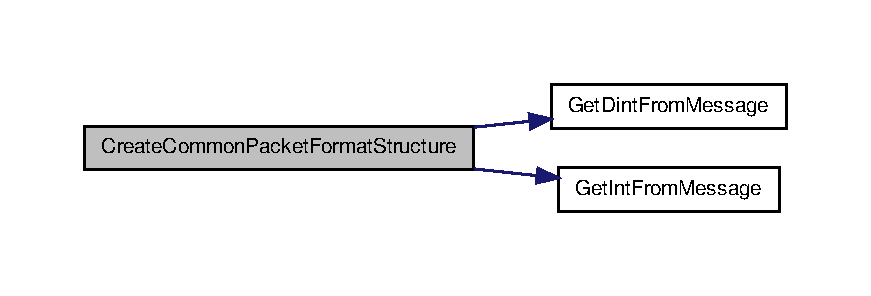
\includegraphics[width=350pt]{d4/d91/group__ENCAP_ga5fd76bfeb985480d68d6fd4d97129606_cgraph}
\end{center}
\end{figure}




\-Here is the caller graph for this function\-:
\nopagebreak
\begin{figure}[H]
\begin{center}
\leavevmode
\includegraphics[width=350pt]{d4/d91/group__ENCAP_ga5fd76bfeb985480d68d6fd4d97129606_icgraph}
\end{center}
\end{figure}


\hypertarget{group__ENCAP_ga7a0dc2be6c485d9e6940d5b20a981022}{\index{\-Op\-E\-Ner Ethernet encapsulation layer@{\-Op\-E\-Ner Ethernet encapsulation layer}!\-Encapsulation\-Init@{\-Encapsulation\-Init}}
\index{\-Encapsulation\-Init@{\-Encapsulation\-Init}!OpENer Ethernet encapsulation layer@{\-Op\-E\-Ner Ethernet encapsulation layer}}
\subsubsection[{\-Encapsulation\-Init}]{\setlength{\rightskip}{0pt plus 5cm}void {\bf \-Encapsulation\-Init} (
\begin{DoxyParamCaption}
\item[{void}]{}
\end{DoxyParamCaption}
)}}\label{d4/d91/group__ENCAP_ga7a0dc2be6c485d9e6940d5b20a981022}


\-Initialize the encapsulation layer. 



\-Definition at line 125 of file encap.\-c.



\-References encapsulation\-\_\-interface\-\_\-information\-::capability\-\_\-flags, \-Determine\-Endianess(), \-E\-N\-C\-A\-P\-\_\-\-N\-U\-M\-B\-E\-R\-\_\-\-O\-F\-\_\-\-S\-U\-P\-P\-O\-R\-T\-E\-D\-\_\-\-D\-E\-L\-A\-Y\-E\-D\-\_\-\-E\-N\-C\-A\-P\-\_\-\-M\-E\-S\-S\-A\-G\-E\-S, encapsulation\-\_\-interface\-\_\-information\-::encapsulation\-\_\-protocol\-\_\-version, g\-\_\-interface\-\_\-information, g\-\_\-registered\-\_\-sessions, \-Cip\-Tcp\-Ip\-Network\-Interface\-Configuration\-::ip\-\_\-address, k\-Capability\-Flags\-Cip\-Tcp, k\-Capability\-Flags\-Cip\-Udp\-Class0or1, k\-Cip\-Item\-Id\-List\-Service\-Response, encapsulation\-\_\-interface\-\_\-information\-::length, encapsulation\-\_\-interface\-\_\-information\-::name\-\_\-of\-\_\-service, \-O\-P\-E\-N\-E\-R\-\_\-\-N\-U\-M\-B\-E\-R\-\_\-\-O\-F\-\_\-\-S\-U\-P\-P\-O\-R\-T\-E\-D\-\_\-\-S\-E\-S\-S\-I\-O\-N\-S, \-Delayed\-Encapsulation\-Message\-::socket, and encapsulation\-\_\-interface\-\_\-information\-::type\-\_\-code.



\-Referenced by \-Cip\-Stack\-Init().



\-Here is the call graph for this function\-:
\nopagebreak
\begin{figure}[H]
\begin{center}
\leavevmode
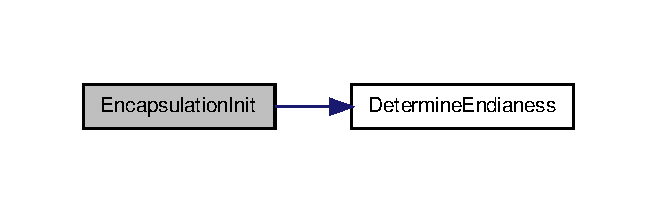
\includegraphics[width=316pt]{d4/d91/group__ENCAP_ga7a0dc2be6c485d9e6940d5b20a981022_cgraph}
\end{center}
\end{figure}




\-Here is the caller graph for this function\-:
\nopagebreak
\begin{figure}[H]
\begin{center}
\leavevmode
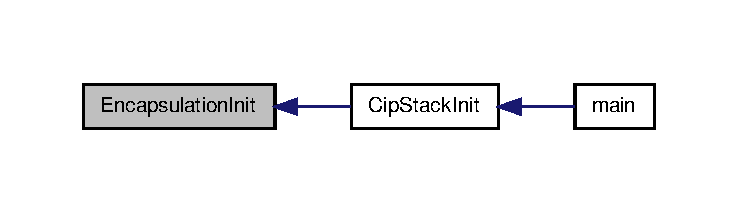
\includegraphics[width=350pt]{d4/d91/group__ENCAP_ga7a0dc2be6c485d9e6940d5b20a981022_icgraph}
\end{center}
\end{figure}


\hypertarget{group__ENCAP_ga1261bd2441f744c38d7a3f8d8c16c391}{\index{\-Op\-E\-Ner Ethernet encapsulation layer@{\-Op\-E\-Ner Ethernet encapsulation layer}!\-Encapsulation\-Shut\-Down@{\-Encapsulation\-Shut\-Down}}
\index{\-Encapsulation\-Shut\-Down@{\-Encapsulation\-Shut\-Down}!OpENer Ethernet encapsulation layer@{\-Op\-E\-Ner Ethernet encapsulation layer}}
\subsubsection[{\-Encapsulation\-Shut\-Down}]{\setlength{\rightskip}{0pt plus 5cm}void {\bf \-Encapsulation\-Shut\-Down} (
\begin{DoxyParamCaption}
\item[{void}]{}
\end{DoxyParamCaption}
)}}\label{d4/d91/group__ENCAP_ga1261bd2441f744c38d7a3f8d8c16c391}


\-Shutdown the encapsulation layer. 

\-This means that all open sessions including their sockets are closed. 

\-Definition at line 632 of file encap.\-c.



\-References g\-\_\-registered\-\_\-sessions, \-I\-App\-\_\-\-Close\-Socket\-\_\-tcp(), and \-O\-P\-E\-N\-E\-R\-\_\-\-N\-U\-M\-B\-E\-R\-\_\-\-O\-F\-\_\-\-S\-U\-P\-P\-O\-R\-T\-E\-D\-\_\-\-S\-E\-S\-S\-I\-O\-N\-S.



\-Referenced by \-Shutdown\-Cip\-Stack().



\-Here is the call graph for this function\-:
\nopagebreak
\begin{figure}[H]
\begin{center}
\leavevmode
\includegraphics[width=350pt]{d4/d91/group__ENCAP_ga1261bd2441f744c38d7a3f8d8c16c391_cgraph}
\end{center}
\end{figure}




\-Here is the caller graph for this function\-:
\nopagebreak
\begin{figure}[H]
\begin{center}
\leavevmode
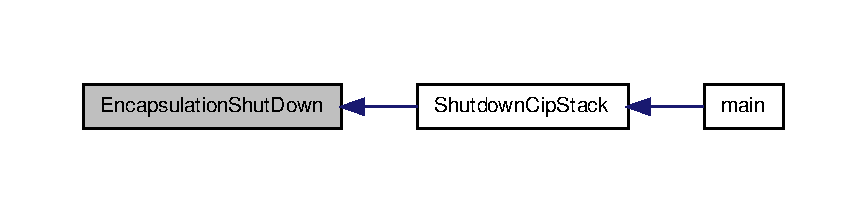
\includegraphics[width=350pt]{d4/d91/group__ENCAP_ga1261bd2441f744c38d7a3f8d8c16c391_icgraph}
\end{center}
\end{figure}


\hypertarget{group__ENCAP_ga668f92389ee06510864585b97955f6f8}{\index{\-Op\-E\-Ner Ethernet encapsulation layer@{\-Op\-E\-Ner Ethernet encapsulation layer}!\-Get\-Dint\-From\-Message@{\-Get\-Dint\-From\-Message}}
\index{\-Get\-Dint\-From\-Message@{\-Get\-Dint\-From\-Message}!OpENer Ethernet encapsulation layer@{\-Op\-E\-Ner Ethernet encapsulation layer}}
\subsubsection[{\-Get\-Dint\-From\-Message}]{\setlength{\rightskip}{0pt plus 5cm}{\bf \-Eip\-Uint32} {\bf \-Get\-Dint\-From\-Message} (
\begin{DoxyParamCaption}
\item[{const {\bf \-Eip\-Uint8} $\ast$$\ast$const}]{buffer}
\end{DoxyParamCaption}
)}}\label{d4/d91/group__ENCAP_ga668f92389ee06510864585b97955f6f8}


\-Get an 32\-Bit integer from the network buffer. 


\begin{DoxyParams}{\-Parameters}
{\em buffer} & pointer to the network buffer array. \-This pointer will be incremented by 4! \\
\hline
\end{DoxyParams}
\begin{DoxyReturn}{\-Returns}
\-Extracted 32 bit integer value
\end{DoxyReturn}
\-Get an 32\-Bit integer from the network buffer.


\begin{DoxyParams}{\-Parameters}
{\em buffer} & pointer where data should be reed. \\
\hline
\end{DoxyParams}
\begin{DoxyReturn}{\-Returns}
\-E\-I\-P\-\_\-\-U\-NÍ\-T32 value 
\end{DoxyReturn}


\-Definition at line 55 of file endianconv.\-c.



\-Referenced by \-Create\-Common\-Packet\-Format\-Structure(), \-Create\-Encapsulation\-Structure(), \-Decode\-Data(), \-Forward\-Close(), \-Forward\-Open(), \-Handle\-Received\-Io\-Connection\-Data(), \-Handle\-Received\-Send\-Request\-Response\-Data\-Command(), and \-Handle\-Received\-Send\-Unit\-Data\-Command().



\-Here is the caller graph for this function\-:
\nopagebreak
\begin{figure}[H]
\begin{center}
\leavevmode
\includegraphics[width=350pt]{d4/d91/group__ENCAP_ga668f92389ee06510864585b97955f6f8_icgraph}
\end{center}
\end{figure}


\hypertarget{group__ENCAP_ga70322f970709ca9c9a1a1d474cfe2302}{\index{\-Op\-E\-Ner Ethernet encapsulation layer@{\-Op\-E\-Ner Ethernet encapsulation layer}!\-Get\-Int\-From\-Message@{\-Get\-Int\-From\-Message}}
\index{\-Get\-Int\-From\-Message@{\-Get\-Int\-From\-Message}!OpENer Ethernet encapsulation layer@{\-Op\-E\-Ner Ethernet encapsulation layer}}
\subsubsection[{\-Get\-Int\-From\-Message}]{\setlength{\rightskip}{0pt plus 5cm}{\bf \-Eip\-Uint16} {\bf \-Get\-Int\-From\-Message} (
\begin{DoxyParamCaption}
\item[{const {\bf \-Eip\-Uint8} $\ast$$\ast$const}]{buffer}
\end{DoxyParamCaption}
)}}\label{d4/d91/group__ENCAP_ga70322f970709ca9c9a1a1d474cfe2302}


\-Get an 16\-Bit integer from the network buffer, and moves pointer beyond the 16 bit value. 


\begin{DoxyParams}{\-Parameters}
{\em buffer} & \-Pointer to the network buffer array. \-This pointer will be incremented by 2! \\
\hline
\end{DoxyParams}
\begin{DoxyReturn}{\-Returns}
\-Extracted 16 bit integer value
\end{DoxyReturn}
\-Get an 16\-Bit integer from the network buffer, and moves pointer beyond the 16 bit value.


\begin{DoxyParams}{\-Parameters}
{\em buffer} & pointer where data should be reed. \\
\hline
\end{DoxyParams}
\begin{DoxyReturn}{\-Returns}
\-E\-I\-P\-\_\-\-U\-I\-N\-T16 data value 
\end{DoxyReturn}


\-Definition at line 43 of file endianconv.\-c.



\-Referenced by \-Create\-Common\-Packet\-Format\-Structure(), \-Create\-Encapsulation\-Structure(), \-Decode\-Data(), \-Decode\-Padded\-E\-Path(), \-Determine\-Delay\-Time(), \-Forward\-Close(), \-Forward\-Open(), \-Handle\-Data\-On\-Tcp\-Socket(), \-Handle\-Received\-Io\-Connection\-Data(), \-Handle\-Received\-Register\-Session\-Command(), \-Handle\-Received\-Send\-Request\-Response\-Data\-Command(), \-Handle\-Received\-Send\-Unit\-Data\-Command(), \-Notify\-Connected\-Common\-Packet\-Format(), and \-Parse\-Connection\-Path().



\-Here is the caller graph for this function\-:
\nopagebreak
\begin{figure}[H]
\begin{center}
\leavevmode
\includegraphics[width=350pt]{d4/d91/group__ENCAP_ga70322f970709ca9c9a1a1d474cfe2302_icgraph}
\end{center}
\end{figure}


\hypertarget{group__ENCAP_ga0a45608ad12bae48152cb1cfafef1a4c}{\index{\-Op\-E\-Ner Ethernet encapsulation layer@{\-Op\-E\-Ner Ethernet encapsulation layer}!\-Get\-Sint\-From\-Message@{\-Get\-Sint\-From\-Message}}
\index{\-Get\-Sint\-From\-Message@{\-Get\-Sint\-From\-Message}!OpENer Ethernet encapsulation layer@{\-Op\-E\-Ner Ethernet encapsulation layer}}
\subsubsection[{\-Get\-Sint\-From\-Message}]{\setlength{\rightskip}{0pt plus 5cm}{\bf \-Eip\-Uint8} {\bf \-Get\-Sint\-From\-Message} (
\begin{DoxyParamCaption}
\item[{const {\bf \-Eip\-Uint8} $\ast$$\ast$const}]{buffer}
\end{DoxyParamCaption}
)}}\label{d4/d91/group__ENCAP_ga0a45608ad12bae48152cb1cfafef1a4c}


\-Reads \-E\-I\-P\-\_\-\-U\-I\-N\-T8 from $\ast$buffer and converts little endian to host. 


\begin{DoxyParams}{\-Parameters}
{\em buffer} & pointer where data should be reed. \\
\hline
\end{DoxyParams}
\begin{DoxyReturn}{\-Returns}
\-E\-I\-P\-\_\-\-U\-I\-N\-T8 data value 
\end{DoxyReturn}


\-Definition at line 29 of file endianconv.\-c.

\hypertarget{group__ENCAP_ga3b9c0d7d9d1413e4cd8ca5634b4bc9ac}{\index{\-Op\-E\-Ner Ethernet encapsulation layer@{\-Op\-E\-Ner Ethernet encapsulation layer}!\-Manage\-Encapsulation\-Messages@{\-Manage\-Encapsulation\-Messages}}
\index{\-Manage\-Encapsulation\-Messages@{\-Manage\-Encapsulation\-Messages}!OpENer Ethernet encapsulation layer@{\-Op\-E\-Ner Ethernet encapsulation layer}}
\subsubsection[{\-Manage\-Encapsulation\-Messages}]{\setlength{\rightskip}{0pt plus 5cm}void {\bf \-Manage\-Encapsulation\-Messages} (
\begin{DoxyParamCaption}
\item[{const {\bf \-Milli\-Seconds}}]{elapsed\-\_\-time}
\end{DoxyParamCaption}
)}}\label{d4/d91/group__ENCAP_ga3b9c0d7d9d1413e4cd8ca5634b4bc9ac}


\-Handle delayed encapsulation message responses. 

\-Certain encapsulation message requests require a delayed sending of the response message. \-This functions checks if messages need to be sent and performs the sending. 

\-Definition at line 641 of file encap.\-c.



\-References \-E\-N\-C\-A\-P\-\_\-\-N\-U\-M\-B\-E\-R\-\_\-\-O\-F\-\_\-\-S\-U\-P\-P\-O\-R\-T\-E\-D\-\_\-\-D\-E\-L\-A\-Y\-E\-D\-\_\-\-E\-N\-C\-A\-P\-\_\-\-M\-E\-S\-S\-A\-G\-E\-S, \-Send\-Udp\-Data(), \-Delayed\-Encapsulation\-Message\-::socket, and \-Delayed\-Encapsulation\-Message\-::time\-\_\-out.



\-Referenced by \-Manage\-Connections().



\-Here is the call graph for this function\-:
\nopagebreak
\begin{figure}[H]
\begin{center}
\leavevmode
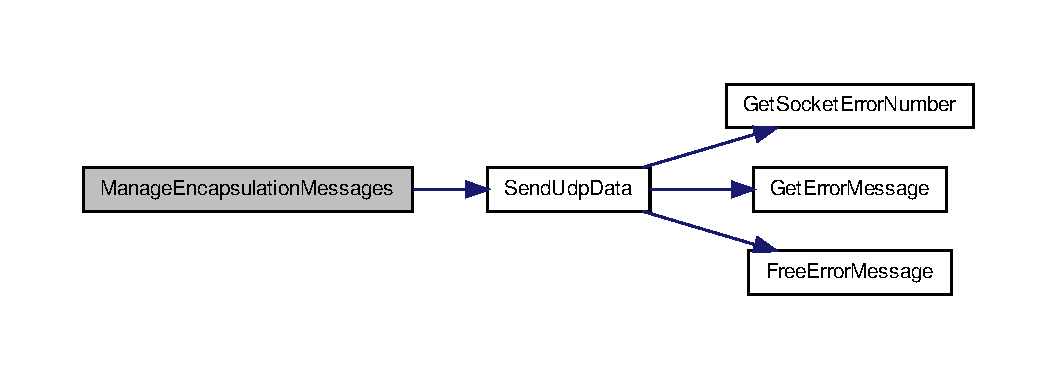
\includegraphics[width=350pt]{d4/d91/group__ENCAP_ga3b9c0d7d9d1413e4cd8ca5634b4bc9ac_cgraph}
\end{center}
\end{figure}




\-Here is the caller graph for this function\-:
\nopagebreak
\begin{figure}[H]
\begin{center}
\leavevmode
\includegraphics[width=350pt]{d4/d91/group__ENCAP_ga3b9c0d7d9d1413e4cd8ca5634b4bc9ac_icgraph}
\end{center}
\end{figure}


\hypertarget{group__ENCAP_ga401f152f47e54b0a6dddcfe723c086f9}{\index{\-Op\-E\-Ner Ethernet encapsulation layer@{\-Op\-E\-Ner Ethernet encapsulation layer}!\-Notify\-Common\-Packet\-Format@{\-Notify\-Common\-Packet\-Format}}
\index{\-Notify\-Common\-Packet\-Format@{\-Notify\-Common\-Packet\-Format}!OpENer Ethernet encapsulation layer@{\-Op\-E\-Ner Ethernet encapsulation layer}}
\subsubsection[{\-Notify\-Common\-Packet\-Format}]{\setlength{\rightskip}{0pt plus 5cm}int {\bf \-Notify\-Common\-Packet\-Format} (
\begin{DoxyParamCaption}
\item[{{\bf \-Encapsulation\-Data} $\ast$const}]{received\-\_\-data, }
\item[{{\bf \-Eip\-Uint8} $\ast$const}]{reply\-\_\-buffer}
\end{DoxyParamCaption}
)}}\label{d4/d91/group__ENCAP_ga401f152f47e54b0a6dddcfe723c086f9}
\-Parse the \-C\-P\-F data from a received unconnected explicit message and hand the data on to the message router


\begin{DoxyParams}{\-Parameters}
{\em received\-\_\-data} & pointer to the encapsulation structure with the received message \\
\hline
{\em reply\-\_\-buffer} & reply buffer \\
\hline
\end{DoxyParams}
\begin{DoxyReturn}{\-Returns}
number of bytes to be sent back. $<$ 0 if nothing should be sent 
\end{DoxyReturn}


\-Definition at line 25 of file cpf.\-c.



\-References \-Cip\-Common\-Packet\-Format\-Data\-::address\-\_\-item, \-Assemble\-Linear\-Message(), \-Create\-Common\-Packet\-Format\-Structure(), encapsulation\-\_\-data\-::current\-\_\-communication\-\_\-buffer\-\_\-position, \-Data\-Item\-::data, \-Cip\-Common\-Packet\-Format\-Data\-::data\-\_\-item, encapsulation\-\_\-data\-::data\-\_\-length, g\-\_\-message\-\_\-router\-\_\-response, k\-Cip\-Item\-Id\-Null\-Address, k\-Cip\-Item\-Id\-Unconnected\-Data\-Item, k\-Eip\-Status\-Error, k\-Eip\-Status\-Ok, k\-Encapsulation\-Protocol\-Incorrect\-Data, \-Data\-Item\-::length, \-Notify\-Message\-Router(), \-O\-P\-E\-N\-E\-R\-\_\-\-T\-R\-A\-C\-E\-\_\-\-E\-R\-R, encapsulation\-\_\-data\-::status, \-Address\-Item\-::type\-\_\-id, and \-Data\-Item\-::type\-\_\-id.



\-Referenced by \-Handle\-Received\-Send\-Request\-Response\-Data\-Command().



\-Here is the call graph for this function\-:
\nopagebreak
\begin{figure}[H]
\begin{center}
\leavevmode
\includegraphics[width=350pt]{d4/d91/group__ENCAP_ga401f152f47e54b0a6dddcfe723c086f9_cgraph}
\end{center}
\end{figure}




\-Here is the caller graph for this function\-:
\nopagebreak
\begin{figure}[H]
\begin{center}
\leavevmode
\includegraphics[width=350pt]{d4/d91/group__ENCAP_ga401f152f47e54b0a6dddcfe723c086f9_icgraph}
\end{center}
\end{figure}


\hypertarget{group__ENCAP_ga045feac9b8747e049e2420df1ec0844b}{\index{\-Op\-E\-Ner Ethernet encapsulation layer@{\-Op\-E\-Ner Ethernet encapsulation layer}!\-Notify\-Connected\-Common\-Packet\-Format@{\-Notify\-Connected\-Common\-Packet\-Format}}
\index{\-Notify\-Connected\-Common\-Packet\-Format@{\-Notify\-Connected\-Common\-Packet\-Format}!OpENer Ethernet encapsulation layer@{\-Op\-E\-Ner Ethernet encapsulation layer}}
\subsubsection[{\-Notify\-Connected\-Common\-Packet\-Format}]{\setlength{\rightskip}{0pt plus 5cm}int {\bf \-Notify\-Connected\-Common\-Packet\-Format} (
\begin{DoxyParamCaption}
\item[{{\bf \-Encapsulation\-Data} $\ast$}]{received\-\_\-data, }
\item[{{\bf \-Eip\-Uint8} $\ast$}]{reply\-\_\-buffer}
\end{DoxyParamCaption}
)}}\label{d4/d91/group__ENCAP_ga045feac9b8747e049e2420df1ec0844b}
\-Parse the \-C\-P\-F data from a received connected explicit message, check the connection status, update any timers, and hand the data on to the message router


\begin{DoxyParams}{\-Parameters}
{\em received\-\_\-data} & pointer to the encapsulation structure with the received message \\
\hline
{\em reply\-\_\-buffer} & reply buffer \\
\hline
\end{DoxyParams}
\begin{DoxyReturn}{\-Returns}
number of bytes to be sent back. $<$ 0 if nothing should be sent 
\end{DoxyReturn}


\-Definition at line 64 of file cpf.\-c.



\-References \-Cip\-Common\-Packet\-Format\-Data\-::address\-\_\-item, \-Assemble\-Linear\-Message(), \-Address\-Data\-::connection\-\_\-identifier, connection\-\_\-object\-::connection\-\_\-timeout\-\_\-multiplier, \-Create\-Common\-Packet\-Format\-Structure(), encapsulation\-\_\-data\-::current\-\_\-communication\-\_\-buffer\-\_\-position, \-Address\-Item\-::data, \-Data\-Item\-::data, \-Cip\-Common\-Packet\-Format\-Data\-::data\-\_\-item, encapsulation\-\_\-data\-::data\-\_\-length, g\-\_\-message\-\_\-router\-\_\-response, \-Get\-Connected\-Object(), \-Get\-Int\-From\-Message(), connection\-\_\-object\-::inactivity\-\_\-watchdog\-\_\-timer, k\-Cip\-Item\-Id\-Connected\-Data\-Item, k\-Cip\-Item\-Id\-Connection\-Address, k\-Eip\-Status\-Error, \-Data\-Item\-::length, \-Notify\-Message\-Router(), connection\-\_\-object\-::o\-\_\-to\-\_\-t\-\_\-requested\-\_\-packet\-\_\-interval, \-O\-P\-E\-N\-E\-R\-\_\-\-T\-R\-A\-C\-E\-\_\-\-E\-R\-R, connection\-\_\-object\-::produced\-\_\-connection\-\_\-id, \-Address\-Data\-::sequence\-\_\-number, \-Address\-Item\-::type\-\_\-id, and \-Data\-Item\-::type\-\_\-id.



\-Referenced by \-Handle\-Received\-Send\-Unit\-Data\-Command().



\-Here is the call graph for this function\-:
\nopagebreak
\begin{figure}[H]
\begin{center}
\leavevmode
\includegraphics[width=350pt]{d4/d91/group__ENCAP_ga045feac9b8747e049e2420df1ec0844b_cgraph}
\end{center}
\end{figure}




\-Here is the caller graph for this function\-:
\nopagebreak
\begin{figure}[H]
\begin{center}
\leavevmode
\includegraphics[width=350pt]{d4/d91/group__ENCAP_ga045feac9b8747e049e2420df1ec0844b_icgraph}
\end{center}
\end{figure}




\subsection{\-Variable \-Documentation}
\hypertarget{group__ENCAP_gafaae5be8de81c633ea4df46fa8b957e0}{\index{\-Op\-E\-Ner Ethernet encapsulation layer@{\-Op\-E\-Ner Ethernet encapsulation layer}!g\-\_\-common\-\_\-packet\-\_\-format\-\_\-data\-\_\-item@{g\-\_\-common\-\_\-packet\-\_\-format\-\_\-data\-\_\-item}}
\index{g\-\_\-common\-\_\-packet\-\_\-format\-\_\-data\-\_\-item@{g\-\_\-common\-\_\-packet\-\_\-format\-\_\-data\-\_\-item}!OpENer Ethernet encapsulation layer@{\-Op\-E\-Ner Ethernet encapsulation layer}}
\subsubsection[{g\-\_\-common\-\_\-packet\-\_\-format\-\_\-data\-\_\-item}]{\setlength{\rightskip}{0pt plus 5cm}{\bf \-Cip\-Common\-Packet\-Format\-Data} {\bf g\-\_\-common\-\_\-packet\-\_\-format\-\_\-data\-\_\-item}}}\label{d4/d91/group__ENCAP_gafaae5be8de81c633ea4df46fa8b957e0}


\-Data storage for the any \-C\-P\-F data \-Currently we are single threaded and need only one \-C\-P\-F at the time. \-For future extensions towards multithreading maybe more \-C\-P\-F data items may be necessary. 

\-C\-P\-F global data items 

\-Definition at line 23 of file cpf.\-c.



\-Referenced by \-Assemble\-Forward\-Close\-Response(), \-Assemble\-Forward\-Open\-Response(), \-Forward\-Close(), \-Handle\-Received\-Connected\-Data(), \-Open\-Communication\-Channels(), \-Open\-Multicast\-Connection(), \-Open\-Producing\-Multicast\-Connection(), and \-Send\-Connected\-Data().


\hypertarget{group__CIP__API}{\section{\-Op\-E\-Ner \-User interface}
\label{d2/dc9/group__CIP__API}\index{\-Op\-E\-Ner User interface@{\-Op\-E\-Ner User interface}}
}


\-This is the public interface of the \-Op\-E\-Ner. \-It provides all function needed to implement an \-Ether\-Net/\-I\-P enabled slave-\/device.  


\-Collaboration diagram for \-Op\-E\-Ner \-User interface\-:
\nopagebreak
\begin{figure}[H]
\begin{center}
\leavevmode
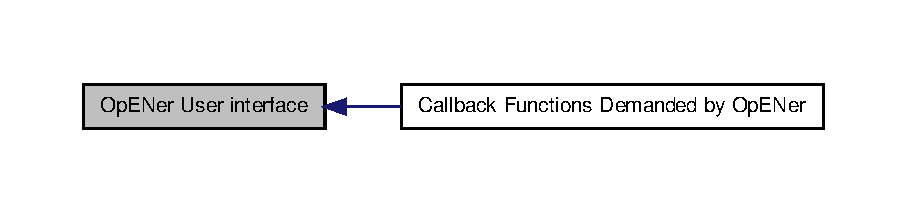
\includegraphics[width=350pt]{d2/dc9/group__CIP__API}
\end{center}
\end{figure}
\subsection*{\-Modules}
\begin{DoxyCompactItemize}
\item 
\hyperlink{group__CIP__CALLBACK__API}{\-Callback Functions Demanded by Op\-E\-Ner}
\begin{DoxyCompactList}\small\item\em \-These functions have to implemented in order to give the \-Op\-E\-Ner a method to inform the application on certain state changes. \end{DoxyCompactList}\end{DoxyCompactItemize}
\subsection*{\-Typedefs}
\begin{DoxyCompactItemize}
\item 
typedef void($\ast$ \hyperlink{group__CIP__API_ga754f77d4872724e212cf1d9d7d84d406}{\-Connection\-Close\-Function} )(struct \hyperlink{structconnection__object}{connection\-\_\-object} $\ast$\hyperlink{structconnection__object}{connection\-\_\-object})
\begin{DoxyCompactList}\small\item\em \-Function prototype for handling the closing of connections. \end{DoxyCompactList}\item 
typedef \hyperlink{typedefs_8h_a3dcc5f7837c120360f8cc88a76781709}{\-Eip\-Status}($\ast$ \hyperlink{group__CIP__API_gaac5ac35ed35317f29e3455e92f450623}{\-Connection\-Receive\-Data\-Function} )(struct \hyperlink{structconnection__object}{connection\-\_\-object} $\ast$\hyperlink{structconnection__object}{connection\-\_\-object}, const \hyperlink{typedefs_8h_aa0c108ee762a27720919a4634643040e}{\-Eip\-Uint8} $\ast$data, const \hyperlink{typedefs_8h_ac1b4cfa25b4f5def62f23b455dd395d8}{\-Eip\-Uint16} data\-\_\-length)
\begin{DoxyCompactList}\small\item\em \-Function prototype for receiving data via a connection. \end{DoxyCompactList}\item 
typedef \hyperlink{typedefs_8h_a3dcc5f7837c120360f8cc88a76781709}{\-Eip\-Status}($\ast$ \hyperlink{group__CIP__API_gaa870412e93039a338e73edc08e9cd68a}{\-Connection\-Send\-Data\-Function} )(struct \hyperlink{structconnection__object}{connection\-\_\-object} $\ast$\hyperlink{structconnection__object}{connection\-\_\-object})
\begin{DoxyCompactList}\small\item\em \-Function prototype for sending data via a connection. \end{DoxyCompactList}\item 
typedef void($\ast$ \hyperlink{group__CIP__API_gaffa28b7ae343af7c7d1c7c52d83bbbee}{\-Connection\-Timeout\-Function} )(struct \hyperlink{structconnection__object}{connection\-\_\-object} $\ast$\hyperlink{structconnection__object}{connection\-\_\-object})
\begin{DoxyCompactList}\small\item\em \-Function prototype for handling the timeout of connections. \end{DoxyCompactList}\item 
typedef \hyperlink{typedefs_8h_a3dcc5f7837c120360f8cc88a76781709}{\-Eip\-Status}($\ast$ \hyperlink{group__CIP__API_gaba609aaaca108b8d1b24da1ccbd7b375}{\-Open\-Connection\-Function} )(\hyperlink{cipconnectionmanager_8h_a705e78f4613ecabcb6388951b73c4700}{\-Connection\-Object} $\ast$\-R\-E\-S\-T\-R\-I\-C\-T const \hyperlink{structconnection__object}{connection\-\_\-object}, \hyperlink{typedefs_8h_ac1b4cfa25b4f5def62f23b455dd395d8}{\-Eip\-Uint16} $\ast$const extended\-\_\-error\-\_\-code)
\begin{DoxyCompactList}\small\item\em \-Function prototype for handling the opening of connections. \end{DoxyCompactList}\end{DoxyCompactItemize}
\subsection*{\-Functions}
\begin{DoxyCompactItemize}
\item 
\hyperlink{ciptypes_8h_aea7976be629e5ece275c993982186188}{\-Cip\-Instance} $\ast$ \hyperlink{group__CIP__API_ga180023c8528628f7d83023e4db81287a}{\-Add\-C\-I\-P\-Instance} (\hyperlink{ciptypes_8h_a175191808b8fac50b47d9bbc9edc6051}{\-Cip\-Class} $\ast$\-R\-E\-S\-T\-R\-I\-C\-T const cip\-\_\-class\-\_\-to\-\_\-add\-\_\-instance, const \hyperlink{typedefs_8h_abf2dd49262551294eb990ef8746a2767}{\-Eip\-Uint32} instance\-\_\-id)
\begin{DoxyCompactList}\small\item\em \-Create one instance of a given class with a certain instance number. \end{DoxyCompactList}\item 
\hyperlink{ciptypes_8h_aea7976be629e5ece275c993982186188}{\-Cip\-Instance} $\ast$ \hyperlink{group__CIP__API_ga39dafca98f844a12511af11b1273d0a8}{\-Add\-Cip\-Instances} (\hyperlink{ciptypes_8h_a175191808b8fac50b47d9bbc9edc6051}{\-Cip\-Class} $\ast$\-R\-E\-S\-T\-R\-I\-C\-T const cip\-\_\-object\-\_\-to\-\_\-add\-\_\-instances, const int number\-\_\-of\-\_\-instances)
\begin{DoxyCompactList}\small\item\em \-Add a number of \-C\-I\-P instances to a given \-C\-I\-P class. \end{DoxyCompactList}\item 
\hyperlink{typedefs_8h_a3dcc5f7837c120360f8cc88a76781709}{\-Eip\-Status} \hyperlink{group__CIP__API_gac7db4d2927e83b6b3110f5dc66589b1e}{\-Add\-Connectable\-Object} (\hyperlink{typedefs_8h_abf2dd49262551294eb990ef8746a2767}{\-Eip\-Uint32} class\-\_\-id, \hyperlink{group__CIP__API_gaba609aaaca108b8d1b24da1ccbd7b375}{\-Open\-Connection\-Function} open\-\_\-connection\-\_\-function)
\begin{DoxyCompactList}\small\item\em register open functions for an specific object. \end{DoxyCompactList}\item 
void \hyperlink{group__CIP__API_ga5d4979945d124e28668b264c3823db1c}{\-Cip\-Stack\-Init} (const \hyperlink{typedefs_8h_ac1b4cfa25b4f5def62f23b455dd395d8}{\-Eip\-Uint16} unique\-\_\-connection\-\_\-id)
\begin{DoxyCompactList}\small\item\em \-Initialize and setup the \-C\-I\-P-\/stack. \end{DoxyCompactList}\item 
void \hyperlink{group__CIP__API_gab9ff230d61fc6dedd90f8b95e9a27707}{\-Close\-Session} (int socket)
\begin{DoxyCompactList}\small\item\em \-Inform the encapsulation layer that the remote host has closed the connection. \end{DoxyCompactList}\item 
void \hyperlink{group__CIP__API_ga388b872aa3290d7248bfbf4b61fc4f1e}{\-Configure\-Domain\-Name} (const char $\ast$const \-R\-E\-S\-T\-R\-I\-C\-T domain\-\_\-name)
\begin{DoxyCompactList}\small\item\em \-Configure the domain name of the device. \end{DoxyCompactList}\item 
void \hyperlink{group__CIP__API_gad1826555a5a2c522bfd98496f31c7ab2}{\-Configure\-Exclusive\-Owner\-Connection\-Point} (const unsigned int connection\-\_\-number, const unsigned int output\-\_\-assembly\-\_\-id, const unsigned int input\-\_\-assembly\-\_\-id, const unsigned int configuration\-\_\-assembly\-\_\-id)
\begin{DoxyCompactList}\small\item\em \-Configures the connection point for an exclusive owner connection. \end{DoxyCompactList}\item 
void \hyperlink{group__CIP__API_gab4a2d826ebe9be1b60c0206414a8f8ce}{\-Configure\-Host\-Name} (const char $\ast$const \-R\-E\-S\-T\-R\-I\-C\-T host\-\_\-name)
\begin{DoxyCompactList}\small\item\em \-Configure the host name of the device. \end{DoxyCompactList}\item 
void \hyperlink{group__CIP__API_ga1f81ca8040f02503c8374288a1453f52}{\-Configure\-Input\-Only\-Connection\-Point} (const unsigned int connection\-\_\-number, const unsigned int output\-\_\-assembly\-\_\-id, const unsigned int input\-\_\-assembly\-\_\-id, const unsigned int configuration\-\_\-assembly\-\_\-id)
\begin{DoxyCompactList}\small\item\em \-Configures the connection point for an input only connection. \end{DoxyCompactList}\item 
void \hyperlink{group__CIP__API_ga0ffe2fb2fa68e86bd2c0b3a94d7ad9bb}{\-Configure\-Listen\-Only\-Connection\-Point} (const unsigned int connection\-\_\-number, const unsigned int output\-\_\-assembly\-\_\-id, const unsigned int input\-\_\-assembly\-\_\-id, const unsigned int configuration\-\_\-assembly\-\_\-id)
\begin{DoxyCompactList}\small\item\em \-Configures the connection point for a listen only connection. \end{DoxyCompactList}\item 
void \hyperlink{group__CIP__API_ga33c5edc60fb8c9b878647ae5e3c03bc5}{\-Configure\-Mac\-Address} (const \hyperlink{typedefs_8h_aa0c108ee762a27720919a4634643040e}{\-Eip\-Uint8} $\ast$const mac\-\_\-address)
\begin{DoxyCompactList}\small\item\em \-Configure the \-M\-A\-C address of the device. \end{DoxyCompactList}\item 
\hyperlink{typedefs_8h_a3dcc5f7837c120360f8cc88a76781709}{\-Eip\-Status} \hyperlink{group__CIP__API_ga1f4f417cb95e75c439edabe7b8b91477}{\-Configure\-Network\-Interface} (const char $\ast$const ip\-\_\-address, const char $\ast$const subnet\-\_\-mask, const char $\ast$const gateway\-\_\-address)
\begin{DoxyCompactList}\small\item\em \-Configure the data of the network interface of the device. \end{DoxyCompactList}\item 
\hyperlink{ciptypes_8h_aea7976be629e5ece275c993982186188}{\-Cip\-Instance} $\ast$ \hyperlink{group__CIP__API_gae61b613fed863d30428e78b2311bf593}{\-Create\-Assembly\-Object} (const \hyperlink{typedefs_8h_abf2dd49262551294eb990ef8746a2767}{\-Eip\-Uint32} instance\-\_\-number, \hyperlink{typedefs_8h_a168bac8db7e7e6d944700e1ac4717ae3}{\-Eip\-Byte} $\ast$const data, const \hyperlink{typedefs_8h_ac1b4cfa25b4f5def62f23b455dd395d8}{\-Eip\-Uint16} data\-\_\-length)
\begin{DoxyCompactList}\small\item\em \-Create an instance of an assembly object. \end{DoxyCompactList}\item 
\hyperlink{ciptypes_8h_a175191808b8fac50b47d9bbc9edc6051}{\-Cip\-Class} $\ast$ \hyperlink{group__CIP__API_ga446b7f612fe7baaf40d7f87274832922}{\-Create\-Cip\-Class} (const \hyperlink{typedefs_8h_abf2dd49262551294eb990ef8746a2767}{\-Eip\-Uint32} class\-\_\-id, const int number\-\_\-of\-\_\-class\-\_\-attributes, const \hyperlink{typedefs_8h_abf2dd49262551294eb990ef8746a2767}{\-Eip\-Uint32} class\-\_\-attributes\-\_\-get\-\_\-attribute\-\_\-all\-\_\-mask, const int number\-\_\-of\-\_\-class\-\_\-services, const int number\-\_\-of\-\_\-instance\-\_\-attributes, const \hyperlink{typedefs_8h_abf2dd49262551294eb990ef8746a2767}{\-Eip\-Uint32} instance\-\_\-attributes\-\_\-get\-\_\-attributes\-\_\-all\-\_\-mask, const int number\-\_\-of\-\_\-instance\-\_\-services, const int number\-\_\-of\-\_\-instances, char $\ast$class\-\_\-name, const \hyperlink{typedefs_8h_ac1b4cfa25b4f5def62f23b455dd395d8}{\-Eip\-Uint16} class\-\_\-revision)
\begin{DoxyCompactList}\small\item\em \-Allocate memory for new \-C\-I\-P \-Class and attributes. \end{DoxyCompactList}\item 
int \hyperlink{group__CIP__API_ga23ef471671180123d441d30895159a3c}{\-Decode\-Data} (const \hyperlink{typedefs_8h_aa0c108ee762a27720919a4634643040e}{\-Eip\-Uint8} cip\-\_\-type, void $\ast$const data, const \hyperlink{typedefs_8h_aa0c108ee762a27720919a4634643040e}{\-Eip\-Uint8} $\ast$$\ast$const message)
\begin{DoxyCompactList}\small\item\em \-Retrieve the given data according to \-C\-I\-P encoding from the message buffer. \end{DoxyCompactList}\item 
int \hyperlink{group__CIP__API_gaece1b7dd2aeec306cb33b86b2ee21980}{\-Encode\-Data} (const \hyperlink{typedefs_8h_aa0c108ee762a27720919a4634643040e}{\-Eip\-Uint8} cip\-\_\-data\-\_\-type, const void $\ast$const cip\-\_\-data, \hyperlink{typedefs_8h_aa0c108ee762a27720919a4634643040e}{\-Eip\-Uint8} $\ast$$\ast$cip\-\_\-message)
\begin{DoxyCompactList}\small\item\em \-Produce the data according to \-C\-I\-P encoding onto the message buffer. \end{DoxyCompactList}\item 
\hyperlink{structCipAttributeStruct}{\-Cip\-Attribute\-Struct} $\ast$ \hyperlink{group__CIP__API_ga5a14c8d76acacb09312b709bb0a76265}{\-Get\-Cip\-Attribute} (const \hyperlink{ciptypes_8h_aea7976be629e5ece275c993982186188}{\-Cip\-Instance} $\ast$const \hyperlink{structcip__instance}{cip\-\_\-instance}, const \hyperlink{typedefs_8h_ac1b4cfa25b4f5def62f23b455dd395d8}{\-Eip\-Uint16} attribute\-\_\-number)
\begin{DoxyCompactList}\small\item\em \-Get a pointer to an instance's attribute. \end{DoxyCompactList}\item 
\hyperlink{ciptypes_8h_a175191808b8fac50b47d9bbc9edc6051}{\-Cip\-Class} $\ast$ \hyperlink{group__CIP__API_ga98bd609c80ece316406363575b4a89ea}{\-Get\-Cip\-Class} (const \hyperlink{typedefs_8h_abf2dd49262551294eb990ef8746a2767}{\-Eip\-Uint32} class\-\_\-id)
\begin{DoxyCompactList}\small\item\em \-Get a pointer to a \-C\-I\-P object with given class code. \end{DoxyCompactList}\item 
\hyperlink{ciptypes_8h_aea7976be629e5ece275c993982186188}{\-Cip\-Instance} $\ast$ \hyperlink{group__CIP__API_gaa50395aca91b378c297d6ad919df210e}{\-Get\-Cip\-Instance} (const \hyperlink{ciptypes_8h_a175191808b8fac50b47d9bbc9edc6051}{\-Cip\-Class} $\ast$\-R\-E\-S\-T\-R\-I\-C\-T const cip\-\_\-object, const \hyperlink{typedefs_8h_abf2dd49262551294eb990ef8746a2767}{\-Eip\-Uint32} instance\-\_\-number)
\begin{DoxyCompactList}\small\item\em \-Get a pointer to an instance. \end{DoxyCompactList}\item 
\hyperlink{typedefs_8h_a3dcc5f7837c120360f8cc88a76781709}{\-Eip\-Status} \hyperlink{group__CIP__API_ga34f1582ed424a2c875b8a317d828e181}{\-Handle\-Received\-Connected\-Data} (\hyperlink{typedefs_8h_aa0c108ee762a27720919a4634643040e}{\-Eip\-Uint8} $\ast$received\-\_\-data, int received\-\_\-data\-\_\-length, struct sockaddr\-\_\-in $\ast$from\-\_\-address)
\begin{DoxyCompactList}\small\item\em \-Notify the connection manager that data for a connection has been received. \end{DoxyCompactList}\item 
int \hyperlink{group__CIP__API_gacbbc9669d41357e1c8497c34ee8eeffb}{\-Handle\-Received\-Explict\-Tcp\-Data} (int socket, \hyperlink{typedefs_8h_aa0c108ee762a27720919a4634643040e}{\-Eip\-Uint8} $\ast$buffer, unsigned int buffer\-\_\-length, int $\ast$number\-\_\-of\-\_\-remaining\-\_\-bytes)
\begin{DoxyCompactList}\small\item\em \-Notify the encapsulation layer that an explicit message has been received via \-T\-C\-P. \end{DoxyCompactList}\item 
int \hyperlink{group__CIP__API_gad2fa74193023adadbbffe5bf0ef7f6ee}{\-Handle\-Received\-Explict\-Udp\-Data} (int socket, struct sockaddr\-\_\-in $\ast$from\-\_\-address, \hyperlink{typedefs_8h_aa0c108ee762a27720919a4634643040e}{\-Eip\-Uint8} $\ast$buffer, unsigned int buffer\-\_\-length, int $\ast$number\-\_\-of\-\_\-remaining\-\_\-bytes, int unicast)
\begin{DoxyCompactList}\small\item\em \-Notify the encapsulation layer that an explicit message has been received via \-U\-D\-P. \end{DoxyCompactList}\item 
void \hyperlink{group__CIP__API_gac207feb53c1f98b45f3934bbea63d618}{\-Insert\-Attribute} (\hyperlink{ciptypes_8h_aea7976be629e5ece275c993982186188}{\-Cip\-Instance} $\ast$const \hyperlink{structcip__instance}{cip\-\_\-instance}, const \hyperlink{typedefs_8h_ac1b4cfa25b4f5def62f23b455dd395d8}{\-Eip\-Uint16} attribute\-\_\-number, const \hyperlink{typedefs_8h_aa0c108ee762a27720919a4634643040e}{\-Eip\-Uint8} cip\-\_\-data\-\_\-type, void $\ast$const cip\-\_\-data, const \hyperlink{typedefs_8h_a168bac8db7e7e6d944700e1ac4717ae3}{\-Eip\-Byte} cip\-\_\-flags)
\begin{DoxyCompactList}\small\item\em \-Insert an attribute in an instance of a \-C\-I\-P class. \end{DoxyCompactList}\item 
void \hyperlink{group__CIP__API_ga35f639b135ec3c3903f49fd65daed307}{\-Insert\-Service} (const \hyperlink{ciptypes_8h_a175191808b8fac50b47d9bbc9edc6051}{\-Cip\-Class} $\ast$const cip\-\_\-class\-\_\-to\-\_\-add\-\_\-service, const \hyperlink{typedefs_8h_aa0c108ee762a27720919a4634643040e}{\-Eip\-Uint8} service\-\_\-code, const \hyperlink{ciptypes_8h_af7606d2a9b86977aa0ac4ec9ccec3701}{\-Cip\-Service\-Function} service\-\_\-function, char $\ast$const service\-\_\-name)
\begin{DoxyCompactList}\small\item\em \-Insert a service in an instance of a \-C\-I\-P object. \end{DoxyCompactList}\item 
\hyperlink{typedefs_8h_a3dcc5f7837c120360f8cc88a76781709}{\-Eip\-Status} \hyperlink{group__CIP__API_ga9f57b09260efb5bfb188b9d0ca0c6091}{\-Manage\-Connections} (\hyperlink{typedefs_8h_a2972c9424f18b12265ca35d0548da82a}{\-Milli\-Seconds} elapsed\-\_\-time)
\begin{DoxyCompactList}\small\item\em \-Check if any of the connection timers (\-Transmission\-Trigger or \-Watchdog\-Timeout) have timed out. \end{DoxyCompactList}\item 
void \hyperlink{group__CIP__API_ga696952d9dbc1b6fdedf517aa55f94323}{\-Set\-Device\-Serial\-Number} (const \hyperlink{typedefs_8h_abf2dd49262551294eb990ef8746a2767}{\-Eip\-Uint32} serial\-\_\-number)
\begin{DoxyCompactList}\small\item\em \-Set the serial number of the device's identity object. \end{DoxyCompactList}\item 
void \hyperlink{group__CIP__API_ga2113be94f1eab4f25770d975abe6015c}{\-Set\-Device\-Status} (const \hyperlink{typedefs_8h_ac1b4cfa25b4f5def62f23b455dd395d8}{\-Eip\-Uint16} device\-\_\-status)
\begin{DoxyCompactList}\small\item\em \-Set the current status of the device. \end{DoxyCompactList}\item 
void \hyperlink{group__CIP__API_gaa57b527530adc2acda6febc500fd6831}{\-Shutdown\-Cip\-Stack} (void)
\begin{DoxyCompactList}\small\item\em \-Shutdown of the \-C\-I\-P stack. \end{DoxyCompactList}\item 
\hyperlink{typedefs_8h_a3dcc5f7837c120360f8cc88a76781709}{\-Eip\-Status} \hyperlink{group__CIP__API_ga286de29d4e88bd1fec0611e75c288faf}{\-Trigger\-Connections} (unsigned int output\-\_\-assembly\-\_\-id, unsigned int input\-\_\-assembly\-\_\-id)
\begin{DoxyCompactList}\small\item\em \-Trigger the production of an application triggered connection. \end{DoxyCompactList}\end{DoxyCompactItemize}


\subsection{\-Detailed \-Description}
\-This is the public interface of the \-Op\-E\-Ner. \-It provides all function needed to implement an \-Ether\-Net/\-I\-P enabled slave-\/device. 

\subsection{\-Typedef \-Documentation}
\hypertarget{group__CIP__API_ga754f77d4872724e212cf1d9d7d84d406}{\index{\-Op\-E\-Ner User interface@{\-Op\-E\-Ner User interface}!\-Connection\-Close\-Function@{\-Connection\-Close\-Function}}
\index{\-Connection\-Close\-Function@{\-Connection\-Close\-Function}!OpENer User interface@{\-Op\-E\-Ner User interface}}
\subsubsection[{\-Connection\-Close\-Function}]{\setlength{\rightskip}{0pt plus 5cm}typedef void($\ast$ {\bf \-Connection\-Close\-Function})(struct {\bf connection\-\_\-object} $\ast${\bf connection\-\_\-object})}}\label{d2/dc9/group__CIP__API_ga754f77d4872724e212cf1d9d7d84d406}


\-Function prototype for handling the closing of connections. 


\begin{DoxyParams}{\-Parameters}
{\em \hyperlink{structconnection__object}{connection\-\_\-object}} & \-The connection object which is closing the connection \\
\hline
\end{DoxyParams}


\-Definition at line 289 of file opener\-\_\-api.\-h.

\hypertarget{group__CIP__API_gaac5ac35ed35317f29e3455e92f450623}{\index{\-Op\-E\-Ner User interface@{\-Op\-E\-Ner User interface}!\-Connection\-Receive\-Data\-Function@{\-Connection\-Receive\-Data\-Function}}
\index{\-Connection\-Receive\-Data\-Function@{\-Connection\-Receive\-Data\-Function}!OpENer User interface@{\-Op\-E\-Ner User interface}}
\subsubsection[{\-Connection\-Receive\-Data\-Function}]{\setlength{\rightskip}{0pt plus 5cm}typedef {\bf \-Eip\-Status}($\ast$ {\bf \-Connection\-Receive\-Data\-Function})(struct {\bf connection\-\_\-object} $\ast${\bf connection\-\_\-object}, const {\bf \-Eip\-Uint8} $\ast$data, const {\bf \-Eip\-Uint16} data\-\_\-length)}}\label{d2/dc9/group__CIP__API_gaac5ac35ed35317f29e3455e92f450623}


\-Function prototype for receiving data via a connection. 


\begin{DoxyParams}{\-Parameters}
{\em \hyperlink{structconnection__object}{connection\-\_\-object}} & \-The connection object which connection timed out \\
\hline
{\em data} & \-The payload of the \-C\-I\-P message \\
\hline
{\em data\-\_\-length} & \-Length of the payload\\
\hline
\end{DoxyParams}
\begin{DoxyReturn}{\-Returns}
\-Stack status 
\end{DoxyReturn}


\-Definition at line 319 of file opener\-\_\-api.\-h.

\hypertarget{group__CIP__API_gaa870412e93039a338e73edc08e9cd68a}{\index{\-Op\-E\-Ner User interface@{\-Op\-E\-Ner User interface}!\-Connection\-Send\-Data\-Function@{\-Connection\-Send\-Data\-Function}}
\index{\-Connection\-Send\-Data\-Function@{\-Connection\-Send\-Data\-Function}!OpENer User interface@{\-Op\-E\-Ner User interface}}
\subsubsection[{\-Connection\-Send\-Data\-Function}]{\setlength{\rightskip}{0pt plus 5cm}typedef {\bf \-Eip\-Status}($\ast$ {\bf \-Connection\-Send\-Data\-Function})(struct {\bf connection\-\_\-object} $\ast${\bf connection\-\_\-object})}}\label{d2/dc9/group__CIP__API_gaa870412e93039a338e73edc08e9cd68a}


\-Function prototype for sending data via a connection. 


\begin{DoxyParams}{\-Parameters}
{\em \hyperlink{structconnection__object}{connection\-\_\-object}} & \-The connection object which connection timed out\\
\hline
\end{DoxyParams}
\begin{DoxyReturn}{\-Returns}
\-E\-I\-P stack status 
\end{DoxyReturn}


\-Definition at line 307 of file opener\-\_\-api.\-h.

\hypertarget{group__CIP__API_gaffa28b7ae343af7c7d1c7c52d83bbbee}{\index{\-Op\-E\-Ner User interface@{\-Op\-E\-Ner User interface}!\-Connection\-Timeout\-Function@{\-Connection\-Timeout\-Function}}
\index{\-Connection\-Timeout\-Function@{\-Connection\-Timeout\-Function}!OpENer User interface@{\-Op\-E\-Ner User interface}}
\subsubsection[{\-Connection\-Timeout\-Function}]{\setlength{\rightskip}{0pt plus 5cm}typedef void($\ast$ {\bf \-Connection\-Timeout\-Function})(struct {\bf connection\-\_\-object} $\ast${\bf connection\-\_\-object})}}\label{d2/dc9/group__CIP__API_gaffa28b7ae343af7c7d1c7c52d83bbbee}


\-Function prototype for handling the timeout of connections. 


\begin{DoxyParams}{\-Parameters}
{\em \hyperlink{structconnection__object}{connection\-\_\-object}} & \-The connection object which connection timed out \\
\hline
\end{DoxyParams}


\-Definition at line 297 of file opener\-\_\-api.\-h.

\hypertarget{group__CIP__API_gaba609aaaca108b8d1b24da1ccbd7b375}{\index{\-Op\-E\-Ner User interface@{\-Op\-E\-Ner User interface}!\-Open\-Connection\-Function@{\-Open\-Connection\-Function}}
\index{\-Open\-Connection\-Function@{\-Open\-Connection\-Function}!OpENer User interface@{\-Op\-E\-Ner User interface}}
\subsubsection[{\-Open\-Connection\-Function}]{\setlength{\rightskip}{0pt plus 5cm}typedef {\bf \-Eip\-Status}($\ast$ {\bf \-Open\-Connection\-Function})({\bf \-Connection\-Object} $\ast$\-R\-E\-S\-T\-R\-I\-C\-T const {\bf connection\-\_\-object}, {\bf \-Eip\-Uint16} $\ast$const extended\-\_\-error\-\_\-code)}}\label{d2/dc9/group__CIP__API_gaba609aaaca108b8d1b24da1ccbd7b375}


\-Function prototype for handling the opening of connections. 


\begin{DoxyParams}{\-Parameters}
{\em \hyperlink{structconnection__object}{connection\-\_\-object}} & \-The connection object which is opening the connection \\
\hline
{\em extended\-\_\-error\-\_\-code} & \-The returned error code of the connection object\\
\hline
\end{DoxyParams}
\begin{DoxyReturn}{\-Returns}
\-C\-I\-P error code 
\end{DoxyReturn}


\-Definition at line 280 of file opener\-\_\-api.\-h.



\subsection{\-Function \-Documentation}
\hypertarget{group__CIP__API_ga180023c8528628f7d83023e4db81287a}{\index{\-Op\-E\-Ner User interface@{\-Op\-E\-Ner User interface}!\-Add\-C\-I\-P\-Instance@{\-Add\-C\-I\-P\-Instance}}
\index{\-Add\-C\-I\-P\-Instance@{\-Add\-C\-I\-P\-Instance}!OpENer User interface@{\-Op\-E\-Ner User interface}}
\subsubsection[{\-Add\-C\-I\-P\-Instance}]{\setlength{\rightskip}{0pt plus 5cm}{\bf \-Cip\-Instance}$\ast$ {\bf \-Add\-C\-I\-P\-Instance} (
\begin{DoxyParamCaption}
\item[{{\bf \-Cip\-Class} $\ast$\-R\-E\-S\-T\-R\-I\-C\-T const}]{cip\-\_\-class\-\_\-to\-\_\-add\-\_\-instance, }
\item[{const {\bf \-Eip\-Uint32}}]{instance\-\_\-id}
\end{DoxyParamCaption}
)}}\label{d2/dc9/group__CIP__API_ga180023c8528628f7d83023e4db81287a}


\-Create one instance of a given class with a certain instance number. 

\-This function can be used for creating out of order instance numbers 
\begin{DoxyParams}{\-Parameters}
{\em pa\-\_\-pst\-C\-I\-P\-Class} & the class the instance should be created for \\
\hline
{\em pa\-\_\-n\-Instance\-Id} & the instance id of the created instance \\
\hline
\end{DoxyParams}
\begin{DoxyReturn}{\-Returns}
pointer to the created instance, if an instance with the given id already exists the existing is returned an no new instance is created 
\end{DoxyReturn}


\-Definition at line 161 of file cipcommon.\-c.



\-References \-Add\-Cip\-Instances(), \-Get\-Cip\-Instance(), and cip\-\_\-instance\-::instance\-\_\-number.



\-Referenced by \-Create\-Assembly\-Object().



\-Here is the call graph for this function\-:
\nopagebreak
\begin{figure}[H]
\begin{center}
\leavevmode
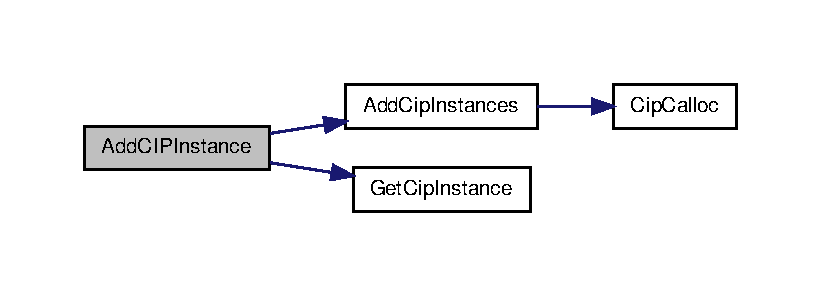
\includegraphics[width=350pt]{d2/dc9/group__CIP__API_ga180023c8528628f7d83023e4db81287a_cgraph}
\end{center}
\end{figure}




\-Here is the caller graph for this function\-:
\nopagebreak
\begin{figure}[H]
\begin{center}
\leavevmode
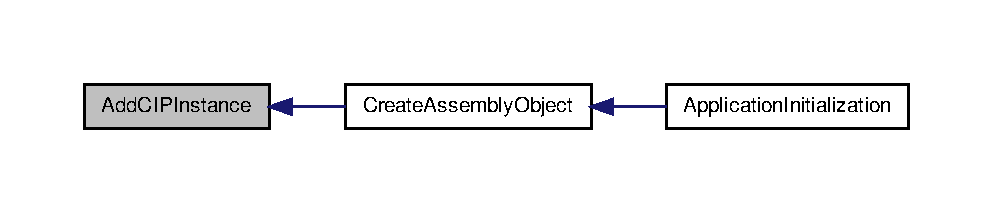
\includegraphics[width=350pt]{d2/dc9/group__CIP__API_ga180023c8528628f7d83023e4db81287a_icgraph}
\end{center}
\end{figure}


\hypertarget{group__CIP__API_ga39dafca98f844a12511af11b1273d0a8}{\index{\-Op\-E\-Ner User interface@{\-Op\-E\-Ner User interface}!\-Add\-Cip\-Instances@{\-Add\-Cip\-Instances}}
\index{\-Add\-Cip\-Instances@{\-Add\-Cip\-Instances}!OpENer User interface@{\-Op\-E\-Ner User interface}}
\subsubsection[{\-Add\-Cip\-Instances}]{\setlength{\rightskip}{0pt plus 5cm}{\bf \-Cip\-Instance}$\ast$ {\bf \-Add\-Cip\-Instances} (
\begin{DoxyParamCaption}
\item[{{\bf \-Cip\-Class} $\ast$\-R\-E\-S\-T\-R\-I\-C\-T const}]{cip\-\_\-object\-\_\-to\-\_\-add\-\_\-instances, }
\item[{const int}]{number\-\_\-of\-\_\-instances}
\end{DoxyParamCaption}
)}}\label{d2/dc9/group__CIP__API_ga39dafca98f844a12511af11b1273d0a8}


\-Add a number of \-C\-I\-P instances to a given \-C\-I\-P class. 

\-The required number of instances are created in a block, but are attached to the class as a linked list. \-The instances are numbered sequentially -\/-\/ i.\-e. the first node in the chain is instance 1, the second is 2, and so on. \-You can add new instances at any time (you do not have to create all the instances of a class at the same time) deleting instances once they have been created is not supported out-\/of-\/order instance numbers are not supported running out of memory while creating new instances causes an assert.


\begin{DoxyParams}{\-Parameters}
{\em cip\-\_\-object\-\_\-to\-\_\-add\-\_\-instances} & \-C\-I\-P object the instances should be added \\
\hline
{\em number\-\_\-of\-\_\-instances} & number of instances to be generated. \\
\hline
\end{DoxyParams}
\begin{DoxyReturn}{\-Returns}
pointer to the first of the new instances 0 on error 
\end{DoxyReturn}


\-Definition at line 117 of file cipcommon.\-c.



\-References cip\-\_\-instance\-::attributes, cip\-\_\-instance\-::cip\-\_\-class, \-Cip\-Calloc(), cip\-\_\-instance\-::instance\-\_\-number, cip\-\_\-instance\-::next, \-O\-P\-E\-N\-E\-R\-\_\-\-A\-S\-S\-E\-R\-T, and \-O\-P\-E\-N\-E\-R\-\_\-\-T\-R\-A\-C\-E\-\_\-\-I\-N\-F\-O.



\-Referenced by \-Add\-C\-I\-P\-Instance(), and \-Create\-Cip\-Class().



\-Here is the call graph for this function\-:
\nopagebreak
\begin{figure}[H]
\begin{center}
\leavevmode
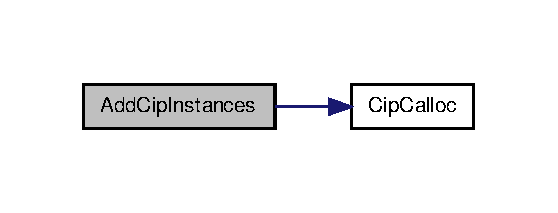
\includegraphics[width=268pt]{d2/dc9/group__CIP__API_ga39dafca98f844a12511af11b1273d0a8_cgraph}
\end{center}
\end{figure}




\-Here is the caller graph for this function\-:
\nopagebreak
\begin{figure}[H]
\begin{center}
\leavevmode
\includegraphics[width=350pt]{d2/dc9/group__CIP__API_ga39dafca98f844a12511af11b1273d0a8_icgraph}
\end{center}
\end{figure}


\hypertarget{group__CIP__API_gac7db4d2927e83b6b3110f5dc66589b1e}{\index{\-Op\-E\-Ner User interface@{\-Op\-E\-Ner User interface}!\-Add\-Connectable\-Object@{\-Add\-Connectable\-Object}}
\index{\-Add\-Connectable\-Object@{\-Add\-Connectable\-Object}!OpENer User interface@{\-Op\-E\-Ner User interface}}
\subsubsection[{\-Add\-Connectable\-Object}]{\setlength{\rightskip}{0pt plus 5cm}{\bf \-Eip\-Status} {\bf \-Add\-Connectable\-Object} (
\begin{DoxyParamCaption}
\item[{{\bf \-Eip\-Uint32}}]{class\-\_\-id, }
\item[{{\bf \-Open\-Connection\-Function}}]{open\-\_\-connection\-\_\-function}
\end{DoxyParamCaption}
)}}\label{d2/dc9/group__CIP__API_gac7db4d2927e83b6b3110f5dc66589b1e}


register open functions for an specific object. 

\-With this function any object can be enabled to be a target for forward open/close request. 
\begin{DoxyParams}{\-Parameters}
{\em class\-\_\-id} & \-The class \-I\-D \\
\hline
{\em open\-\_\-connection\-\_\-function} & pointer to the function handling the open process \\
\hline
\end{DoxyParams}
\begin{DoxyReturn}{\-Returns}
\-E\-I\-P\-\_\-\-O\-K on success 
\end{DoxyReturn}


\-Definition at line 1205 of file cipconnectionmanager.\-c.



\-References \-Connection\-Management\-Handling\-::class\-\_\-id, k\-Eip\-Status\-Error, k\-Eip\-Status\-Ok, and \-Connection\-Management\-Handling\-::open\-\_\-connection\-\_\-function.



\-Referenced by \-Connection\-Manager\-Init().



\-Here is the caller graph for this function\-:
\nopagebreak
\begin{figure}[H]
\begin{center}
\leavevmode
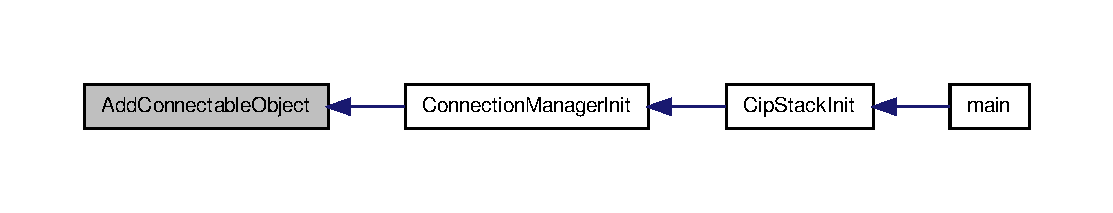
\includegraphics[width=350pt]{d2/dc9/group__CIP__API_gac7db4d2927e83b6b3110f5dc66589b1e_icgraph}
\end{center}
\end{figure}


\hypertarget{group__CIP__API_ga5d4979945d124e28668b264c3823db1c}{\index{\-Op\-E\-Ner User interface@{\-Op\-E\-Ner User interface}!\-Cip\-Stack\-Init@{\-Cip\-Stack\-Init}}
\index{\-Cip\-Stack\-Init@{\-Cip\-Stack\-Init}!OpENer User interface@{\-Op\-E\-Ner User interface}}
\subsubsection[{\-Cip\-Stack\-Init}]{\setlength{\rightskip}{0pt plus 5cm}void {\bf \-Cip\-Stack\-Init} (
\begin{DoxyParamCaption}
\item[{const {\bf \-Eip\-Uint16}}]{unique\-\_\-connection\-\_\-id}
\end{DoxyParamCaption}
)}}\label{d2/dc9/group__CIP__API_ga5d4979945d124e28668b264c3823db1c}


\-Initialize and setup the \-C\-I\-P-\/stack. 


\begin{DoxyParams}{\-Parameters}
{\em unique\-\_\-connection\-\_\-id} & value passed to \-Connection\-\_\-\-Manager\-\_\-\-Init() to form a \char`\"{}per boot\char`\"{} unique connection \-I\-D. \\
\hline
\end{DoxyParams}


\-Definition at line 33 of file cipcommon.\-c.



\-References \-Application\-Initialization(), \-Cip\-Assembly\-Initialize(), \-Cip\-Ethernet\-Link\-Init(), \-Cip\-Identity\-Init(), \-Cip\-Message\-Router\-Init(), \-Cip\-Tcp\-Ip\-Interface\-Init(), \-Connection\-Manager\-Init(), \-Encapsulation\-Init(), k\-Eip\-Status\-Ok, and \-O\-P\-E\-N\-E\-R\-\_\-\-A\-S\-S\-E\-R\-T.



\-Referenced by main().



\-Here is the call graph for this function\-:
\nopagebreak
\begin{figure}[H]
\begin{center}
\leavevmode
\includegraphics[width=350pt]{d2/dc9/group__CIP__API_ga5d4979945d124e28668b264c3823db1c_cgraph}
\end{center}
\end{figure}




\-Here is the caller graph for this function\-:
\nopagebreak
\begin{figure}[H]
\begin{center}
\leavevmode
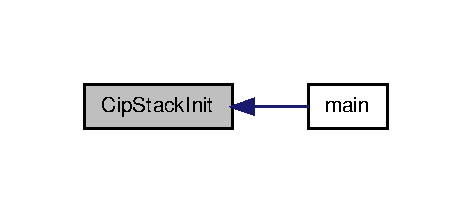
\includegraphics[width=226pt]{d2/dc9/group__CIP__API_ga5d4979945d124e28668b264c3823db1c_icgraph}
\end{center}
\end{figure}


\hypertarget{group__CIP__API_gab9ff230d61fc6dedd90f8b95e9a27707}{\index{\-Op\-E\-Ner User interface@{\-Op\-E\-Ner User interface}!\-Close\-Session@{\-Close\-Session}}
\index{\-Close\-Session@{\-Close\-Session}!OpENer User interface@{\-Op\-E\-Ner User interface}}
\subsubsection[{\-Close\-Session}]{\setlength{\rightskip}{0pt plus 5cm}void {\bf \-Close\-Session} (
\begin{DoxyParamCaption}
\item[{int}]{socket}
\end{DoxyParamCaption}
)}}\label{d2/dc9/group__CIP__API_gab9ff230d61fc6dedd90f8b95e9a27707}


\-Inform the encapsulation layer that the remote host has closed the connection. 

\-According to the specifications that will clean up and close the session in the encapsulation layer. 
\begin{DoxyParams}{\-Parameters}
{\em socket\-\_\-handle} & the handler to the socket of the closed connection \\
\hline
\end{DoxyParams}


\-Definition at line 621 of file encap.\-c.



\-References g\-\_\-registered\-\_\-sessions, \-I\-App\-\_\-\-Close\-Socket\-\_\-tcp(), and \-O\-P\-E\-N\-E\-R\-\_\-\-N\-U\-M\-B\-E\-R\-\_\-\-O\-F\-\_\-\-S\-U\-P\-P\-O\-R\-T\-E\-D\-\_\-\-S\-E\-S\-S\-I\-O\-N\-S.



\-Referenced by \-Network\-Handler\-Process\-Once().



\-Here is the call graph for this function\-:
\nopagebreak
\begin{figure}[H]
\begin{center}
\leavevmode
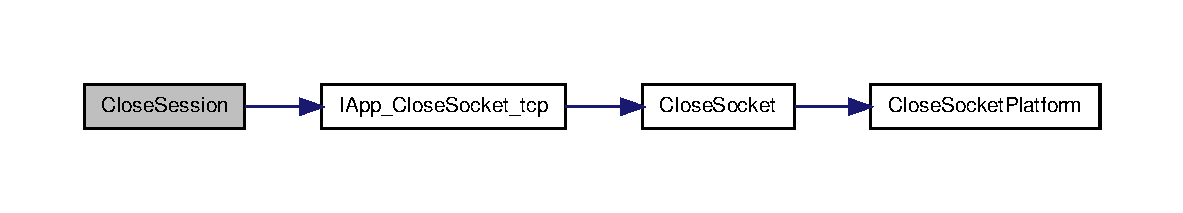
\includegraphics[width=350pt]{d2/dc9/group__CIP__API_gab9ff230d61fc6dedd90f8b95e9a27707_cgraph}
\end{center}
\end{figure}




\-Here is the caller graph for this function\-:
\nopagebreak
\begin{figure}[H]
\begin{center}
\leavevmode
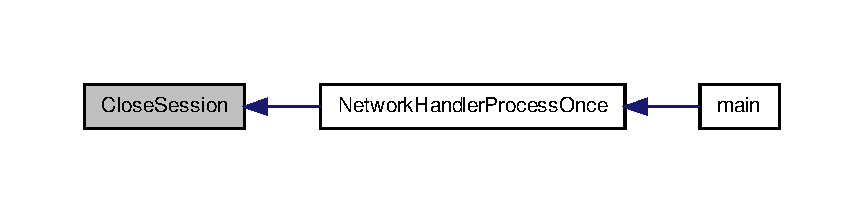
\includegraphics[width=350pt]{d2/dc9/group__CIP__API_gab9ff230d61fc6dedd90f8b95e9a27707_icgraph}
\end{center}
\end{figure}


\hypertarget{group__CIP__API_ga388b872aa3290d7248bfbf4b61fc4f1e}{\index{\-Op\-E\-Ner User interface@{\-Op\-E\-Ner User interface}!\-Configure\-Domain\-Name@{\-Configure\-Domain\-Name}}
\index{\-Configure\-Domain\-Name@{\-Configure\-Domain\-Name}!OpENer User interface@{\-Op\-E\-Ner User interface}}
\subsubsection[{\-Configure\-Domain\-Name}]{\setlength{\rightskip}{0pt plus 5cm}void {\bf \-Configure\-Domain\-Name} (
\begin{DoxyParamCaption}
\item[{const char $\ast$const \-R\-E\-S\-T\-R\-I\-C\-T}]{domain\-\_\-name}
\end{DoxyParamCaption}
)}}\label{d2/dc9/group__CIP__API_ga388b872aa3290d7248bfbf4b61fc4f1e}


\-Configure the domain name of the device. 


\begin{DoxyParams}{\-Parameters}
{\em domain\-\_\-name} & the domain name to be used \\
\hline
\end{DoxyParams}


\-Definition at line 85 of file ciptcpipinterface.\-c.



\-References \-Cip\-Calloc(), \-Cip\-Free(), \-Cip\-Tcp\-Ip\-Network\-Interface\-Configuration\-::domain\-\_\-name, \-Cip\-String\-::length, and \-Cip\-String\-::string.



\-Referenced by main().



\-Here is the call graph for this function\-:
\nopagebreak
\begin{figure}[H]
\begin{center}
\leavevmode
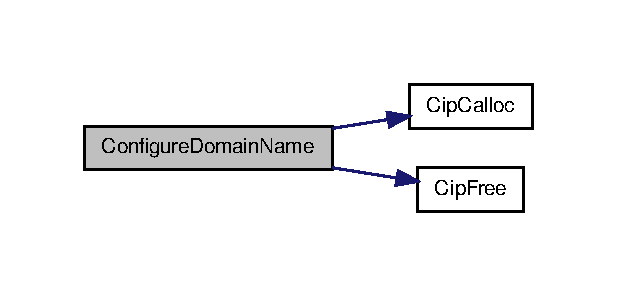
\includegraphics[width=296pt]{d2/dc9/group__CIP__API_ga388b872aa3290d7248bfbf4b61fc4f1e_cgraph}
\end{center}
\end{figure}




\-Here is the caller graph for this function\-:
\nopagebreak
\begin{figure}[H]
\begin{center}
\leavevmode
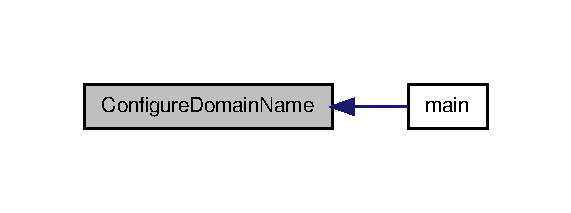
\includegraphics[width=274pt]{d2/dc9/group__CIP__API_ga388b872aa3290d7248bfbf4b61fc4f1e_icgraph}
\end{center}
\end{figure}


\hypertarget{group__CIP__API_gad1826555a5a2c522bfd98496f31c7ab2}{\index{\-Op\-E\-Ner User interface@{\-Op\-E\-Ner User interface}!\-Configure\-Exclusive\-Owner\-Connection\-Point@{\-Configure\-Exclusive\-Owner\-Connection\-Point}}
\index{\-Configure\-Exclusive\-Owner\-Connection\-Point@{\-Configure\-Exclusive\-Owner\-Connection\-Point}!OpENer User interface@{\-Op\-E\-Ner User interface}}
\subsubsection[{\-Configure\-Exclusive\-Owner\-Connection\-Point}]{\setlength{\rightskip}{0pt plus 5cm}void {\bf \-Configure\-Exclusive\-Owner\-Connection\-Point} (
\begin{DoxyParamCaption}
\item[{const unsigned int}]{connection\-\_\-number, }
\item[{const unsigned int}]{output\-\_\-assembly\-\_\-id, }
\item[{const unsigned int}]{input\-\_\-assembly\-\_\-id, }
\item[{const unsigned int}]{configuration\-\_\-assembly\-\_\-id}
\end{DoxyParamCaption}
)}}\label{d2/dc9/group__CIP__API_gad1826555a5a2c522bfd98496f31c7ab2}


\-Configures the connection point for an exclusive owner connection. 


\begin{DoxyParams}{\-Parameters}
{\em connection\-\_\-number} & \-The number of the exclusive owner connection. \-The enumeration starts with 0. \-Has to be smaller than \-O\-P\-E\-N\-E\-R\-\_\-\-C\-I\-P\-\_\-\-N\-U\-M\-\_\-\-E\-X\-L\-U\-S\-I\-V\-E\-\_\-\-O\-W\-N\-E\-R\-\_\-\-C\-O\-N\-N\-S. \\
\hline
{\em output\-\_\-assembly\-\_\-id} & \-I\-D of the \-O-\/to-\/\-T point to be used for this connection \\
\hline
{\em input\-\_\-assembly\-\_\-id} & \-I\-D of the \-T-\/to-\/\-O point to be used for this connection \\
\hline
{\em configuration\-\_\-assembly\-\_\-id} & \-I\-D of the configuration point to be used for this connection \\
\hline
\end{DoxyParams}


\-Definition at line 57 of file appcontype.\-c.



\-References \-Exclusive\-Owner\-Connection\-::config\-\_\-assembly, \-Exclusive\-Owner\-Connection\-::input\-\_\-assembly, \-O\-P\-E\-N\-E\-R\-\_\-\-C\-I\-P\-\_\-\-N\-U\-M\-\_\-\-E\-X\-L\-U\-S\-I\-V\-E\-\_\-\-O\-W\-N\-E\-R\-\_\-\-C\-O\-N\-N\-S, and \-Exclusive\-Owner\-Connection\-::output\-\_\-assembly.



\-Referenced by \-Application\-Initialization().



\-Here is the caller graph for this function\-:
\nopagebreak
\begin{figure}[H]
\begin{center}
\leavevmode
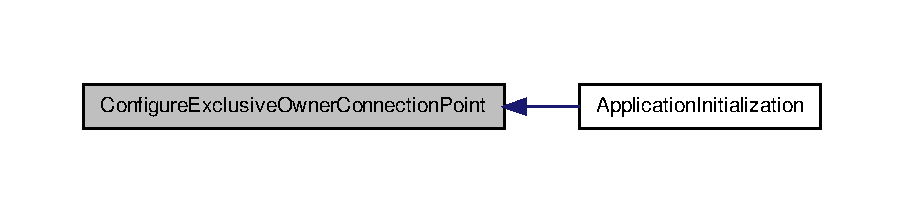
\includegraphics[width=350pt]{d2/dc9/group__CIP__API_gad1826555a5a2c522bfd98496f31c7ab2_icgraph}
\end{center}
\end{figure}


\hypertarget{group__CIP__API_gab4a2d826ebe9be1b60c0206414a8f8ce}{\index{\-Op\-E\-Ner User interface@{\-Op\-E\-Ner User interface}!\-Configure\-Host\-Name@{\-Configure\-Host\-Name}}
\index{\-Configure\-Host\-Name@{\-Configure\-Host\-Name}!OpENer User interface@{\-Op\-E\-Ner User interface}}
\subsubsection[{\-Configure\-Host\-Name}]{\setlength{\rightskip}{0pt plus 5cm}void {\bf \-Configure\-Host\-Name} (
\begin{DoxyParamCaption}
\item[{const char $\ast$const \-R\-E\-S\-T\-R\-I\-C\-T}]{host\-\_\-name}
\end{DoxyParamCaption}
)}}\label{d2/dc9/group__CIP__API_gab4a2d826ebe9be1b60c0206414a8f8ce}


\-Configure the host name of the device. 


\begin{DoxyParams}{\-Parameters}
{\em host\-\_\-name} & the host name to be used \\
\hline
\end{DoxyParams}


\-Definition at line 102 of file ciptcpipinterface.\-c.



\-References \-Cip\-Calloc(), \-Cip\-Free(), \-Cip\-String\-::length, and \-Cip\-String\-::string.



\-Referenced by main().



\-Here is the call graph for this function\-:
\nopagebreak
\begin{figure}[H]
\begin{center}
\leavevmode
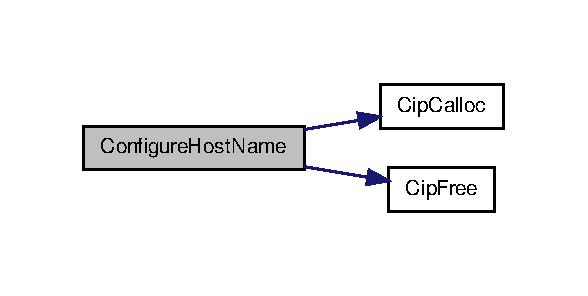
\includegraphics[width=282pt]{d2/dc9/group__CIP__API_gab4a2d826ebe9be1b60c0206414a8f8ce_cgraph}
\end{center}
\end{figure}




\-Here is the caller graph for this function\-:
\nopagebreak
\begin{figure}[H]
\begin{center}
\leavevmode
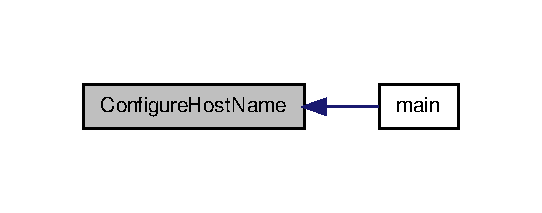
\includegraphics[width=260pt]{d2/dc9/group__CIP__API_gab4a2d826ebe9be1b60c0206414a8f8ce_icgraph}
\end{center}
\end{figure}


\hypertarget{group__CIP__API_ga1f81ca8040f02503c8374288a1453f52}{\index{\-Op\-E\-Ner User interface@{\-Op\-E\-Ner User interface}!\-Configure\-Input\-Only\-Connection\-Point@{\-Configure\-Input\-Only\-Connection\-Point}}
\index{\-Configure\-Input\-Only\-Connection\-Point@{\-Configure\-Input\-Only\-Connection\-Point}!OpENer User interface@{\-Op\-E\-Ner User interface}}
\subsubsection[{\-Configure\-Input\-Only\-Connection\-Point}]{\setlength{\rightskip}{0pt plus 5cm}void {\bf \-Configure\-Input\-Only\-Connection\-Point} (
\begin{DoxyParamCaption}
\item[{const unsigned int}]{connection\-\_\-number, }
\item[{const unsigned int}]{output\-\_\-assembly\-\_\-id, }
\item[{const unsigned int}]{input\-\_\-assembly\-\_\-id, }
\item[{const unsigned int}]{configuration\-\_\-assembly\-\_\-id}
\end{DoxyParamCaption}
)}}\label{d2/dc9/group__CIP__API_ga1f81ca8040f02503c8374288a1453f52}


\-Configures the connection point for an input only connection. 


\begin{DoxyParams}{\-Parameters}
{\em connection\-\_\-number} & \-The number of the input only connection. \-The enumeration starts with 0. \-Has to be smaller than \-O\-P\-E\-N\-E\-R\-\_\-\-C\-I\-P\-\_\-\-N\-U\-M\-\_\-\-I\-N\-P\-U\-T\-\_\-\-O\-N\-L\-Y\-\_\-\-C\-O\-N\-N\-S. \\
\hline
{\em output\-\_\-assembly\-\_\-id} & \-I\-D of the \-O-\/to-\/\-T point to be used for this connection \\
\hline
{\em input\-\_\-assembly\-\_\-id} & \-I\-D of the \-T-\/to-\/\-O point to be used for this connection \\
\hline
{\em configuration\-\_\-assembly\-\_\-id} & \-I\-D of the configuration point to be used for this connection \\
\hline
\end{DoxyParams}


\-Definition at line 71 of file appcontype.\-c.



\-References \-Input\-Only\-Connection\-::config\-\_\-assembly, \-Input\-Only\-Connection\-::input\-\_\-assembly, \-O\-P\-E\-N\-E\-R\-\_\-\-C\-I\-P\-\_\-\-N\-U\-M\-\_\-\-I\-N\-P\-U\-T\-\_\-\-O\-N\-L\-Y\-\_\-\-C\-O\-N\-N\-S, and \-Input\-Only\-Connection\-::output\-\_\-assembly.



\-Referenced by \-Application\-Initialization().



\-Here is the caller graph for this function\-:
\nopagebreak
\begin{figure}[H]
\begin{center}
\leavevmode
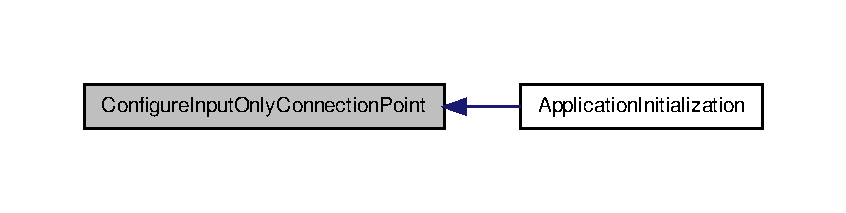
\includegraphics[width=350pt]{d2/dc9/group__CIP__API_ga1f81ca8040f02503c8374288a1453f52_icgraph}
\end{center}
\end{figure}


\hypertarget{group__CIP__API_ga0ffe2fb2fa68e86bd2c0b3a94d7ad9bb}{\index{\-Op\-E\-Ner User interface@{\-Op\-E\-Ner User interface}!\-Configure\-Listen\-Only\-Connection\-Point@{\-Configure\-Listen\-Only\-Connection\-Point}}
\index{\-Configure\-Listen\-Only\-Connection\-Point@{\-Configure\-Listen\-Only\-Connection\-Point}!OpENer User interface@{\-Op\-E\-Ner User interface}}
\subsubsection[{\-Configure\-Listen\-Only\-Connection\-Point}]{\setlength{\rightskip}{0pt plus 5cm}void {\bf \-Configure\-Listen\-Only\-Connection\-Point} (
\begin{DoxyParamCaption}
\item[{const unsigned int}]{connection\-\_\-number, }
\item[{const unsigned int}]{output\-\_\-assembly\-\_\-id, }
\item[{const unsigned int}]{input\-\_\-assembly\-\_\-id, }
\item[{const unsigned int}]{configuration\-\_\-assembly\-\_\-id}
\end{DoxyParamCaption}
)}}\label{d2/dc9/group__CIP__API_ga0ffe2fb2fa68e86bd2c0b3a94d7ad9bb}


\-Configures the connection point for a listen only connection. 


\begin{DoxyParams}{\-Parameters}
{\em connection\-\_\-number} & \-The number of the input only connection. \-The enumeration starts with 0. \-Has to be smaller than \-O\-P\-E\-N\-E\-R\-\_\-\-C\-I\-P\-\_\-\-N\-U\-M\-\_\-\-L\-I\-S\-T\-E\-N\-\_\-\-O\-N\-L\-Y\-\_\-\-C\-O\-N\-N\-S. \\
\hline
{\em output\-\_\-assembly\-\_\-id} & \-I\-D of the \-O-\/to-\/\-T point to be used for this connection \\
\hline
{\em input\-\_\-assembly\-\_\-id} & \-I\-D of the \-T-\/to-\/\-O point to be used for this connection \\
\hline
{\em configuration\-\_\-assembly\-\_\-id} & \-I\-D of the configuration point to be used for this connection \\
\hline
\end{DoxyParams}


\-Definition at line 84 of file appcontype.\-c.



\-References \-Listen\-Only\-Connection\-::config\-\_\-assembly, \-Listen\-Only\-Connection\-::input\-\_\-assembly, \-O\-P\-E\-N\-E\-R\-\_\-\-C\-I\-P\-\_\-\-N\-U\-M\-\_\-\-L\-I\-S\-T\-E\-N\-\_\-\-O\-N\-L\-Y\-\_\-\-C\-O\-N\-N\-S, and \-Listen\-Only\-Connection\-::output\-\_\-assembly.



\-Referenced by \-Application\-Initialization().



\-Here is the caller graph for this function\-:
\nopagebreak
\begin{figure}[H]
\begin{center}
\leavevmode
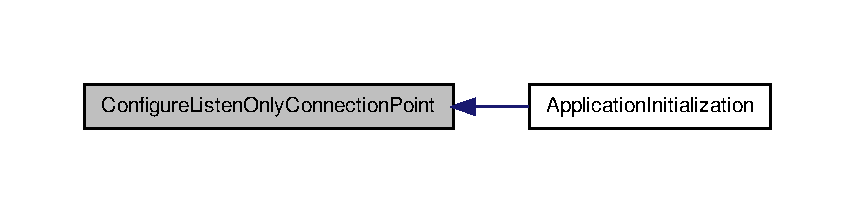
\includegraphics[width=350pt]{d2/dc9/group__CIP__API_ga0ffe2fb2fa68e86bd2c0b3a94d7ad9bb_icgraph}
\end{center}
\end{figure}


\hypertarget{group__CIP__API_ga33c5edc60fb8c9b878647ae5e3c03bc5}{\index{\-Op\-E\-Ner User interface@{\-Op\-E\-Ner User interface}!\-Configure\-Mac\-Address@{\-Configure\-Mac\-Address}}
\index{\-Configure\-Mac\-Address@{\-Configure\-Mac\-Address}!OpENer User interface@{\-Op\-E\-Ner User interface}}
\subsubsection[{\-Configure\-Mac\-Address}]{\setlength{\rightskip}{0pt plus 5cm}void {\bf \-Configure\-Mac\-Address} (
\begin{DoxyParamCaption}
\item[{const {\bf \-Eip\-Uint8} $\ast$const}]{mac\-\_\-address}
\end{DoxyParamCaption}
)}}\label{d2/dc9/group__CIP__API_ga33c5edc60fb8c9b878647ae5e3c03bc5}


\-Configure the \-M\-A\-C address of the device. 


\begin{DoxyParams}{\-Parameters}
{\em mac\-\_\-address} & the hardware \-M\-A\-C address of the network interface\\
\hline
\end{DoxyParams}
\-Configures the \-M\-A\-C address of the \-Ethernet \-Link object$\ast$


\begin{DoxyParams}{\-Parameters}
{\em mac\-\_\-address} & \-The \-M\-A\-C address of the \-Ethernet \-Link \\
\hline
\end{DoxyParams}


\-Definition at line 30 of file cipethernetlink.\-c.



\-References \-Cip\-Ethernet\-Link\-Object\-::physical\-\_\-address.



\-Referenced by main().



\-Here is the caller graph for this function\-:
\nopagebreak
\begin{figure}[H]
\begin{center}
\leavevmode
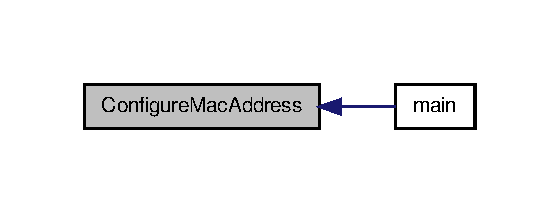
\includegraphics[width=268pt]{d2/dc9/group__CIP__API_ga33c5edc60fb8c9b878647ae5e3c03bc5_icgraph}
\end{center}
\end{figure}


\hypertarget{group__CIP__API_ga1f4f417cb95e75c439edabe7b8b91477}{\index{\-Op\-E\-Ner User interface@{\-Op\-E\-Ner User interface}!\-Configure\-Network\-Interface@{\-Configure\-Network\-Interface}}
\index{\-Configure\-Network\-Interface@{\-Configure\-Network\-Interface}!OpENer User interface@{\-Op\-E\-Ner User interface}}
\subsubsection[{\-Configure\-Network\-Interface}]{\setlength{\rightskip}{0pt plus 5cm}{\bf \-Eip\-Status} {\bf \-Configure\-Network\-Interface} (
\begin{DoxyParamCaption}
\item[{const char $\ast$const}]{ip\-\_\-address, }
\item[{const char $\ast$const}]{subnet\-\_\-mask, }
\item[{const char $\ast$const}]{gateway\-\_\-address}
\end{DoxyParamCaption}
)}}\label{d2/dc9/group__CIP__API_ga1f4f417cb95e75c439edabe7b8b91477}


\-Configure the data of the network interface of the device. 

\-This function setup the data of the network interface needed by \-Op\-E\-Ner. \-The multicast address is automatically calculated from he given data.


\begin{DoxyParams}{\-Parameters}
{\em ip\-\_\-address} & the current \-I\-P address of the device \\
\hline
{\em subnet\-\_\-mask} & the subnet mask to be used \\
\hline
{\em gateway\-\_\-address} & the gateway address \\
\hline
\end{DoxyParams}
\begin{DoxyReturn}{\-Returns}
\-E\-I\-P\-\_\-\-O\-K if the configuring worked otherwise \-E\-I\-P\-\_\-\-E\-R\-R\-O\-R 
\end{DoxyReturn}


\-Definition at line 65 of file ciptcpipinterface.\-c.



\-References \-Cip\-Tcp\-Ip\-Network\-Interface\-Configuration\-::gateway, \-Cip\-Tcp\-Ip\-Network\-Interface\-Configuration\-::ip\-\_\-address, k\-Eip\-Status\-Ok, \-Cip\-Tcp\-Ip\-Network\-Interface\-Configuration\-::network\-\_\-mask, and multicast\-\_\-address\-\_\-configuration\-::starting\-\_\-multicast\-\_\-address.



\-Referenced by main().



\-Here is the caller graph for this function\-:
\nopagebreak
\begin{figure}[H]
\begin{center}
\leavevmode
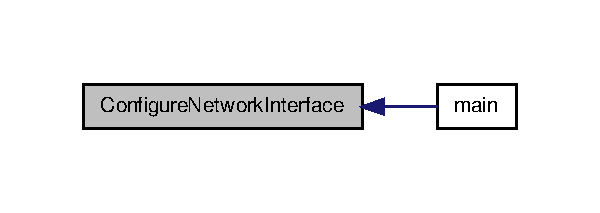
\includegraphics[width=288pt]{d2/dc9/group__CIP__API_ga1f4f417cb95e75c439edabe7b8b91477_icgraph}
\end{center}
\end{figure}


\hypertarget{group__CIP__API_gae61b613fed863d30428e78b2311bf593}{\index{\-Op\-E\-Ner User interface@{\-Op\-E\-Ner User interface}!\-Create\-Assembly\-Object@{\-Create\-Assembly\-Object}}
\index{\-Create\-Assembly\-Object@{\-Create\-Assembly\-Object}!OpENer User interface@{\-Op\-E\-Ner User interface}}
\subsubsection[{\-Create\-Assembly\-Object}]{\setlength{\rightskip}{0pt plus 5cm}{\bf \-Cip\-Instance}$\ast$ {\bf \-Create\-Assembly\-Object} (
\begin{DoxyParamCaption}
\item[{const {\bf \-Eip\-Uint32}}]{instance\-\_\-number, }
\item[{{\bf \-Eip\-Byte} $\ast$const}]{data, }
\item[{const {\bf \-Eip\-Uint16}}]{data\-\_\-length}
\end{DoxyParamCaption}
)}}\label{d2/dc9/group__CIP__API_gae61b613fed863d30428e78b2311bf593}


\-Create an instance of an assembly object. 


\begin{DoxyParams}{\-Parameters}
{\em instance\-\_\-number} & instance number of the assembly object to create \\
\hline
{\em data} & pointer to the data the assembly object should contain \\
\hline
{\em data\-\_\-length} & length of the assembly object's data \\
\hline
\end{DoxyParams}
\begin{DoxyReturn}{\-Returns}
pointer to the instance of the created assembly object. \-N\-U\-L\-L on error
\end{DoxyReturn}
\-Assembly \-Objects for \-Configuration \-Data\-:

\-The \-C\-I\-P stack treats configuration assembly objects the same way as any other assembly object. \-In order to support a configuration assembly object it has to be created with this function. \-The notification on received configuration data is handled with the \-I\-App\-\_\-after\-\_\-receive function. 

\-Definition at line 71 of file cipassembly.\-c.



\-References \-Add\-C\-I\-P\-Instance(), \-Cip\-Calloc(), \-Create\-Assembly\-Class(), \-Cip\-Byte\-Array\-::data, \-Get\-Cip\-Class(), \-Insert\-Attribute(), k\-Cip\-Byte\-Array, k\-Cip\-Uint, k\-Getable\-Single, k\-Set\-And\-Get\-Able, and \-Cip\-Byte\-Array\-::length.



\-Referenced by \-Application\-Initialization().



\-Here is the call graph for this function\-:
\nopagebreak
\begin{figure}[H]
\begin{center}
\leavevmode
\includegraphics[width=350pt]{d2/dc9/group__CIP__API_gae61b613fed863d30428e78b2311bf593_cgraph}
\end{center}
\end{figure}




\-Here is the caller graph for this function\-:
\nopagebreak
\begin{figure}[H]
\begin{center}
\leavevmode
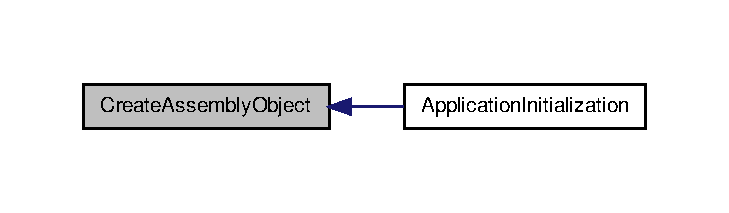
\includegraphics[width=350pt]{d2/dc9/group__CIP__API_gae61b613fed863d30428e78b2311bf593_icgraph}
\end{center}
\end{figure}


\hypertarget{group__CIP__API_ga446b7f612fe7baaf40d7f87274832922}{\index{\-Op\-E\-Ner User interface@{\-Op\-E\-Ner User interface}!\-Create\-Cip\-Class@{\-Create\-Cip\-Class}}
\index{\-Create\-Cip\-Class@{\-Create\-Cip\-Class}!OpENer User interface@{\-Op\-E\-Ner User interface}}
\subsubsection[{\-Create\-Cip\-Class}]{\setlength{\rightskip}{0pt plus 5cm}{\bf \-Cip\-Class}$\ast$ {\bf \-Create\-Cip\-Class} (
\begin{DoxyParamCaption}
\item[{const {\bf \-Eip\-Uint32}}]{class\-\_\-id, }
\item[{const int}]{number\-\_\-of\-\_\-class\-\_\-attributes, }
\item[{const {\bf \-Eip\-Uint32}}]{class\-\_\-attributes\-\_\-get\-\_\-attribute\-\_\-all\-\_\-mask, }
\item[{const int}]{number\-\_\-of\-\_\-class\-\_\-services, }
\item[{const int}]{number\-\_\-of\-\_\-instance\-\_\-attributes, }
\item[{const {\bf \-Eip\-Uint32}}]{instance\-\_\-attributes\-\_\-get\-\_\-attributes\-\_\-all\-\_\-mask, }
\item[{const int}]{number\-\_\-of\-\_\-instance\-\_\-services, }
\item[{const int}]{number\-\_\-of\-\_\-instances, }
\item[{char $\ast$}]{class\-\_\-name, }
\item[{const {\bf \-Eip\-Uint16}}]{class\-\_\-revision}
\end{DoxyParamCaption}
)}}\label{d2/dc9/group__CIP__API_ga446b7f612fe7baaf40d7f87274832922}


\-Allocate memory for new \-C\-I\-P \-Class and attributes. 

\-The new \-C\-I\-P class will be registered at the stack to be able for receiving explicit messages.


\begin{DoxyParams}{\-Parameters}
{\em class\-\_\-id} & class \-I\-D of the new class \\
\hline
{\em number\-\_\-of\-\_\-class\-\_\-attributes} & number of class attributes \\
\hline
{\em get\-\_\-attribute\-\_\-all\-\_\-mask} & mask of which attributes are included in the class get\-Attribute\-All. \-If the mask is 0 the get\-Attribute\-All service will not be added as class service \\
\hline
{\em number\-\_\-of\-\_\-class\-\_\-services} & number of class services \\
\hline
{\em number\-\_\-of\-\_\-instance\-\_\-attributes} & number of attributes of each instance \\
\hline
{\em instance\-\_\-attributes\-\_\-get\-\_\-attributes\-\_\-all\-\_\-mask} & mask of which attributes are included in the instance get\-Attribute\-All \-If the mask is 0 the get\-Attribute\-All service will not be added as class service \\
\hline
{\em number\-\_\-of\-\_\-instance\-\_\-services} & number of instance services \\
\hline
{\em number\-\_\-of\-\_\-instances} & number of initial instances to create \\
\hline
{\em class\-\_\-name} & class name (for debugging class structure) \\
\hline
{\em class\-\_\-revision} & class revision \\
\hline
\end{DoxyParams}
\begin{DoxyReturn}{\-Returns}
pointer to new class object 0 on error 
\end{DoxyReturn}


\-Definition at line 171 of file cipcommon.\-c.



\-References \-Add\-Cip\-Instances(), \-Cip\-Calloc(), cip\-\_\-class\-::class\-\_\-id, \-Get\-Attribute\-All(), \-Get\-Attribute\-Single(), \-Get\-Cip\-Class(), \-Insert\-Attribute(), \-Insert\-Service(), k\-Cip\-Uint, k\-Cip\-Uint\-Zero, k\-Eip\-Status\-Error, k\-Getable\-All, k\-Getable\-Single\-And\-All, k\-Get\-Attribute\-All, k\-Get\-Attribute\-Single, \-O\-P\-E\-N\-E\-R\-\_\-\-A\-S\-S\-E\-R\-T, \-O\-P\-E\-N\-E\-R\-\_\-\-T\-R\-A\-C\-E\-\_\-\-I\-N\-F\-O, \-Register\-Cip\-Class(), and cip\-\_\-class\-::revision.



\-Referenced by \-Cip\-Ethernet\-Link\-Init(), \-Cip\-Identity\-Init(), \-Cip\-Message\-Router\-Init(), \-Cip\-Tcp\-Ip\-Interface\-Init(), \-Connection\-Manager\-Init(), and \-Create\-Assembly\-Class().



\-Here is the call graph for this function\-:
\nopagebreak
\begin{figure}[H]
\begin{center}
\leavevmode
\includegraphics[width=350pt]{d2/dc9/group__CIP__API_ga446b7f612fe7baaf40d7f87274832922_cgraph}
\end{center}
\end{figure}




\-Here is the caller graph for this function\-:
\nopagebreak
\begin{figure}[H]
\begin{center}
\leavevmode
\includegraphics[width=350pt]{d2/dc9/group__CIP__API_ga446b7f612fe7baaf40d7f87274832922_icgraph}
\end{center}
\end{figure}


\hypertarget{group__CIP__API_ga23ef471671180123d441d30895159a3c}{\index{\-Op\-E\-Ner User interface@{\-Op\-E\-Ner User interface}!\-Decode\-Data@{\-Decode\-Data}}
\index{\-Decode\-Data@{\-Decode\-Data}!OpENer User interface@{\-Op\-E\-Ner User interface}}
\subsubsection[{\-Decode\-Data}]{\setlength{\rightskip}{0pt plus 5cm}int {\bf \-Decode\-Data} (
\begin{DoxyParamCaption}
\item[{const {\bf \-Eip\-Uint8}}]{cip\-\_\-type, }
\item[{void $\ast$const}]{data, }
\item[{const {\bf \-Eip\-Uint8} $\ast$$\ast$const}]{message}
\end{DoxyParamCaption}
)}}\label{d2/dc9/group__CIP__API_ga23ef471671180123d441d30895159a3c}


\-Retrieve the given data according to \-C\-I\-P encoding from the message buffer. 

\-This function may be used in in own services for handling data from the requester (e.\-g., set\-Attribute\-Single). 
\begin{DoxyParams}{\-Parameters}
{\em cip\-\_\-data\-\_\-type} & the \-C\-I\-P type to decode \\
\hline
{\em cip\-\_\-data} & pointer to data value to written. \\
\hline
{\em cip\-\_\-message} & pointer to memory where the data should be taken from \\
\hline
\end{DoxyParams}
\begin{DoxyReturn}{\-Returns}
length of taken bytes -\/1 .. error 
\end{DoxyReturn}


\-Definition at line 562 of file cipcommon.\-c.



\-References \-Get\-Dint\-From\-Message(), \-Get\-Int\-From\-Message(), k\-Cip\-Bool, k\-Cip\-Byte, k\-Cip\-Dint, k\-Cip\-Dword, k\-Cip\-Int, k\-Cip\-Lint, k\-Cip\-Lword, k\-Cip\-Short\-String, k\-Cip\-Sint, k\-Cip\-String, k\-Cip\-Udint, k\-Cip\-Uint, k\-Cip\-Ulint, k\-Cip\-Usint, k\-Cip\-Word, \-Cip\-Short\-String\-::length, \-Cip\-String\-::length, \-Cip\-Short\-String\-::string, and \-Cip\-String\-::string.



\-Here is the call graph for this function\-:
\nopagebreak
\begin{figure}[H]
\begin{center}
\leavevmode
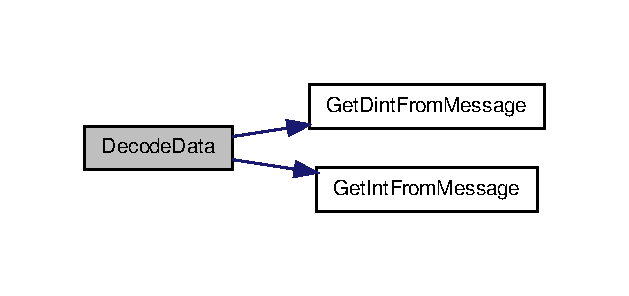
\includegraphics[width=302pt]{d2/dc9/group__CIP__API_ga23ef471671180123d441d30895159a3c_cgraph}
\end{center}
\end{figure}


\hypertarget{group__CIP__API_gaece1b7dd2aeec306cb33b86b2ee21980}{\index{\-Op\-E\-Ner User interface@{\-Op\-E\-Ner User interface}!\-Encode\-Data@{\-Encode\-Data}}
\index{\-Encode\-Data@{\-Encode\-Data}!OpENer User interface@{\-Op\-E\-Ner User interface}}
\subsubsection[{\-Encode\-Data}]{\setlength{\rightskip}{0pt plus 5cm}int {\bf \-Encode\-Data} (
\begin{DoxyParamCaption}
\item[{const {\bf \-Eip\-Uint8}}]{cip\-\_\-data\-\_\-type, }
\item[{const void $\ast$const}]{cip\-\_\-data, }
\item[{{\bf \-Eip\-Uint8} $\ast$$\ast$}]{cip\-\_\-message}
\end{DoxyParamCaption}
)}}\label{d2/dc9/group__CIP__API_gaece1b7dd2aeec306cb33b86b2ee21980}


\-Produce the data according to \-C\-I\-P encoding onto the message buffer. 

\-This function may be used in own services for sending data back to the requester (e.\-g., get\-Attribute\-Single for special structs). 
\begin{DoxyParams}{\-Parameters}
{\em cip\-\_\-data\-\_\-type} & the cip type to encode \\
\hline
{\em cip\-\_\-data} & pointer to data value. \\
\hline
{\em cip\-\_\-message} & pointer to memory where response should be written \\
\hline
\end{DoxyParams}
\begin{DoxyReturn}{\-Returns}
length of attribute in bytes -\/1 .. error 
\end{DoxyReturn}


\-Definition at line 404 of file cipcommon.\-c.



\-References \-Add\-Dint\-To\-Message(), \-Add\-Int\-To\-Message(), \-Add\-Sint\-To\-Message(), \-Cip\-Byte\-Array\-::data, \-Cip\-Tcp\-Ip\-Network\-Interface\-Configuration\-::domain\-\_\-name, \-Encode\-Data(), \-Encode\-E\-Path(), \-Cip\-Tcp\-Ip\-Network\-Interface\-Configuration\-::gateway, \-Cip\-Tcp\-Ip\-Network\-Interface\-Configuration\-::ip\-\_\-address, k\-Cip6\-Usint, k\-Cip\-Bool, k\-Cip\-Byte, k\-Cip\-Byte\-Array, k\-Cip\-Date, k\-Cip\-Date\-And\-Time, k\-Cip\-Dint, k\-Cip\-Dword, k\-Cip\-Eng\-Unit, k\-Cip\-Epath, k\-Cip\-Ftime, k\-Cip\-Int, k\-Cip\-Itime, k\-Cip\-Lint, k\-Cip\-Lreal, k\-Cip\-Ltime, k\-Cip\-Lword, k\-Cip\-Member\-List, k\-Cip\-Real, k\-Cip\-Short\-String, k\-Cip\-Sint, k\-Cip\-Stime, k\-Cip\-String, k\-Cip\-String2, k\-Cip\-String\-N, k\-Cip\-Time, k\-Cip\-Time\-Of\-Day, k\-Cip\-Udint, k\-Cip\-Udint\-Udint\-Udint\-Udint\-Udint\-String, k\-Cip\-Uint, k\-Cip\-Ulint, k\-Cip\-Usint, k\-Cip\-Usint\-Usint, k\-Cip\-Word, k\-Internal\-Uint6, \-Cip\-Byte\-Array\-::length, \-Cip\-Short\-String\-::length, \-Cip\-String\-::length, \-Cip\-Revision\-::major\-\_\-revision, \-Cip\-Revision\-::minor\-\_\-revision, \-Cip\-Tcp\-Ip\-Network\-Interface\-Configuration\-::name\-\_\-server, \-Cip\-Tcp\-Ip\-Network\-Interface\-Configuration\-::name\-\_\-server\-\_\-2, \-Cip\-Tcp\-Ip\-Network\-Interface\-Configuration\-::network\-\_\-mask, \-O\-P\-E\-N\-E\-R\-\_\-\-T\-R\-A\-C\-E\-\_\-\-I\-N\-F\-O, cip\-\_\-class\-::revision, \-Cip\-Short\-String\-::string, and \-Cip\-String\-::string.



\-Referenced by \-Encode\-Data(), \-Get\-Attribute\-Single(), and \-Get\-Attribute\-Single\-Tcp\-Ip\-Interface().



\-Here is the call graph for this function\-:
\nopagebreak
\begin{figure}[H]
\begin{center}
\leavevmode
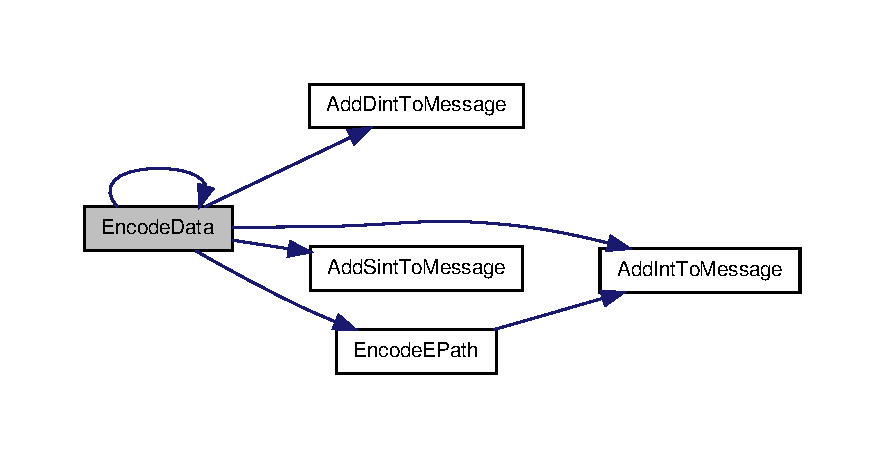
\includegraphics[width=350pt]{d2/dc9/group__CIP__API_gaece1b7dd2aeec306cb33b86b2ee21980_cgraph}
\end{center}
\end{figure}




\-Here is the caller graph for this function\-:
\nopagebreak
\begin{figure}[H]
\begin{center}
\leavevmode
\includegraphics[width=350pt]{d2/dc9/group__CIP__API_gaece1b7dd2aeec306cb33b86b2ee21980_icgraph}
\end{center}
\end{figure}


\hypertarget{group__CIP__API_ga5a14c8d76acacb09312b709bb0a76265}{\index{\-Op\-E\-Ner User interface@{\-Op\-E\-Ner User interface}!\-Get\-Cip\-Attribute@{\-Get\-Cip\-Attribute}}
\index{\-Get\-Cip\-Attribute@{\-Get\-Cip\-Attribute}!OpENer User interface@{\-Op\-E\-Ner User interface}}
\subsubsection[{\-Get\-Cip\-Attribute}]{\setlength{\rightskip}{0pt plus 5cm}{\bf \-Cip\-Attribute\-Struct}$\ast$ {\bf \-Get\-Cip\-Attribute} (
\begin{DoxyParamCaption}
\item[{const {\bf \-Cip\-Instance} $\ast$const}]{cip\-\_\-instance, }
\item[{const {\bf \-Eip\-Uint16}}]{attribute\-\_\-number}
\end{DoxyParamCaption}
)}}\label{d2/dc9/group__CIP__API_ga5a14c8d76acacb09312b709bb0a76265}


\-Get a pointer to an instance's attribute. 

\-As instances and objects are selfsimilar this function can also be used to retrieve the attribute of an object. 
\begin{DoxyParams}{\-Parameters}
{\em \hyperlink{structcip__instance}{cip\-\_\-instance}} & pointer to the instance the attribute belongs to \\
\hline
{\em attribute\-\_\-number} & number of the attribute to retrieve \\
\hline
\end{DoxyParams}
\begin{DoxyReturn}{\-Returns}
pointer to attribute 0 if instance is not in the object 
\end{DoxyReturn}


\-Definition at line 336 of file cipcommon.\-c.



\-References \-Cip\-Attribute\-Struct\-::attribute\-\_\-number, cip\-\_\-instance\-::attributes, cip\-\_\-instance\-::cip\-\_\-class, cip\-\_\-class\-::number\-\_\-of\-\_\-attributes, and \-O\-P\-E\-N\-E\-R\-\_\-\-T\-R\-A\-C\-E\-\_\-\-W\-A\-R\-N.



\-Referenced by \-Establish\-Io\-Connction(), \-Get\-Attribute\-Single(), \-Handle\-Config\-Data(), \-Set\-Assembly\-Attribute\-Single(), \-Set\-Attribute\-Single\-Tcp(), and \-Shutdown\-Assemblies().



\-Here is the caller graph for this function\-:
\nopagebreak
\begin{figure}[H]
\begin{center}
\leavevmode
\includegraphics[width=350pt]{d2/dc9/group__CIP__API_ga5a14c8d76acacb09312b709bb0a76265_icgraph}
\end{center}
\end{figure}


\hypertarget{group__CIP__API_ga98bd609c80ece316406363575b4a89ea}{\index{\-Op\-E\-Ner User interface@{\-Op\-E\-Ner User interface}!\-Get\-Cip\-Class@{\-Get\-Cip\-Class}}
\index{\-Get\-Cip\-Class@{\-Get\-Cip\-Class}!OpENer User interface@{\-Op\-E\-Ner User interface}}
\subsubsection[{\-Get\-Cip\-Class}]{\setlength{\rightskip}{0pt plus 5cm}{\bf \-Cip\-Class}$\ast$ {\bf \-Get\-Cip\-Class} (
\begin{DoxyParamCaption}
\item[{const {\bf \-Eip\-Uint32}}]{class\-\_\-id}
\end{DoxyParamCaption}
)}}\label{d2/dc9/group__CIP__API_ga98bd609c80ece316406363575b4a89ea}


\-Get a pointer to a \-C\-I\-P object with given class code. 


\begin{DoxyParams}{\-Parameters}
{\em class\-\_\-id} & class \-I\-D of the object to retrieve \\
\hline
\end{DoxyParams}
\begin{DoxyReturn}{\-Returns}
pointer to \-C\-I\-P \-Object 0 if object is not present in the stack 
\end{DoxyReturn}


\-Definition at line 92 of file cipmessagerouter.\-c.



\-References cip\-\_\-message\-\_\-router\-\_\-object\-::cip\-\_\-class, and \-Get\-Registered\-Object().



\-Referenced by \-Create\-Assembly\-Object(), \-Create\-Cip\-Class(), \-Establish\-Io\-Connction(), \-Parse\-Connection\-Path(), and \-Shutdown\-Assemblies().



\-Here is the call graph for this function\-:
\nopagebreak
\begin{figure}[H]
\begin{center}
\leavevmode
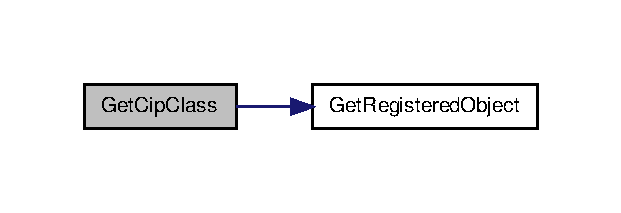
\includegraphics[width=298pt]{d2/dc9/group__CIP__API_ga98bd609c80ece316406363575b4a89ea_cgraph}
\end{center}
\end{figure}




\-Here is the caller graph for this function\-:
\nopagebreak
\begin{figure}[H]
\begin{center}
\leavevmode
\includegraphics[width=350pt]{d2/dc9/group__CIP__API_ga98bd609c80ece316406363575b4a89ea_icgraph}
\end{center}
\end{figure}


\hypertarget{group__CIP__API_gaa50395aca91b378c297d6ad919df210e}{\index{\-Op\-E\-Ner User interface@{\-Op\-E\-Ner User interface}!\-Get\-Cip\-Instance@{\-Get\-Cip\-Instance}}
\index{\-Get\-Cip\-Instance@{\-Get\-Cip\-Instance}!OpENer User interface@{\-Op\-E\-Ner User interface}}
\subsubsection[{\-Get\-Cip\-Instance}]{\setlength{\rightskip}{0pt plus 5cm}{\bf \-Cip\-Instance}$\ast$ {\bf \-Get\-Cip\-Instance} (
\begin{DoxyParamCaption}
\item[{const {\bf \-Cip\-Class} $\ast$\-R\-E\-S\-T\-R\-I\-C\-T const}]{cip\-\_\-object, }
\item[{const {\bf \-Eip\-Uint32}}]{instance\-\_\-number}
\end{DoxyParamCaption}
)}}\label{d2/dc9/group__CIP__API_gaa50395aca91b378c297d6ad919df210e}


\-Get a pointer to an instance. 


\begin{DoxyParams}{\-Parameters}
{\em cip\-\_\-object} & pointer to the object the instance belongs to \\
\hline
{\em instance\-\_\-number} & number of the instance to retrieve \\
\hline
\end{DoxyParams}
\begin{DoxyReturn}{\-Returns}
pointer to \-C\-I\-P \-Instance 0 if instance is not in the object 
\end{DoxyReturn}


\-Definition at line 101 of file cipmessagerouter.\-c.



\-References cip\-\_\-message\-\_\-router\-\_\-object\-::cip\-\_\-class, and cip\-\_\-instance\-::next.



\-Referenced by \-Add\-C\-I\-P\-Instance(), \-Cip\-Ethernet\-Link\-Init(), \-Cip\-Identity\-Init(), \-Cip\-Tcp\-Ip\-Interface\-Init(), \-Establish\-Io\-Connction(), \-Handle\-Config\-Data(), \-Notify\-Class(), and \-Parse\-Connection\-Path().



\-Here is the caller graph for this function\-:
\nopagebreak
\begin{figure}[H]
\begin{center}
\leavevmode
\includegraphics[width=350pt]{d2/dc9/group__CIP__API_gaa50395aca91b378c297d6ad919df210e_icgraph}
\end{center}
\end{figure}


\hypertarget{group__CIP__API_ga34f1582ed424a2c875b8a317d828e181}{\index{\-Op\-E\-Ner User interface@{\-Op\-E\-Ner User interface}!\-Handle\-Received\-Connected\-Data@{\-Handle\-Received\-Connected\-Data}}
\index{\-Handle\-Received\-Connected\-Data@{\-Handle\-Received\-Connected\-Data}!OpENer User interface@{\-Op\-E\-Ner User interface}}
\subsubsection[{\-Handle\-Received\-Connected\-Data}]{\setlength{\rightskip}{0pt plus 5cm}{\bf \-Eip\-Status} {\bf \-Handle\-Received\-Connected\-Data} (
\begin{DoxyParamCaption}
\item[{{\bf \-Eip\-Uint8} $\ast$}]{received\-\_\-data, }
\item[{int}]{received\-\_\-data\-\_\-length, }
\item[{struct sockaddr\-\_\-in $\ast$}]{from\-\_\-address}
\end{DoxyParamCaption}
)}}\label{d2/dc9/group__CIP__API_ga34f1582ed424a2c875b8a317d828e181}


\-Notify the connection manager that data for a connection has been received. 

\-This function should be invoked by the network layer. 
\begin{DoxyParams}{\-Parameters}
{\em received\-\_\-data} & pointer to the buffer of data that has been received \\
\hline
{\em received\-\_\-data\-\_\-length} & number of bytes in the data buffer \\
\hline
{\em from\-\_\-address} & address from which the data has been received. \-Only data from the connections originator may be accepted. \-Avoids connection hijacking \\
\hline
\end{DoxyParams}
\begin{DoxyReturn}{\-Returns}
\-E\-I\-P\-\_\-\-O\-K on success 
\end{DoxyReturn}


\-Definition at line 199 of file cipconnectionmanager.\-c.



\-References \-Cip\-Common\-Packet\-Format\-Data\-::address\-\_\-item, \-Address\-Data\-::connection\-\_\-identifier, connection\-\_\-object\-::connection\-\_\-receive\-\_\-data\-\_\-function, connection\-\_\-object\-::connection\-\_\-timeout\-\_\-multiplier, \-Create\-Common\-Packet\-Format\-Structure(), \-Address\-Item\-::data, \-Data\-Item\-::data, \-Cip\-Common\-Packet\-Format\-Data\-::data\-\_\-item, connection\-\_\-object\-::eip\-\_\-level\-\_\-sequence\-\_\-count\-\_\-consuming, g\-\_\-common\-\_\-packet\-\_\-format\-\_\-data\-\_\-item, \-Get\-Connected\-Object(), connection\-\_\-object\-::inactivity\-\_\-watchdog\-\_\-timer, k\-Cip\-Item\-Id\-Connected\-Data\-Item, k\-Cip\-Item\-Id\-Connection\-Address, k\-Cip\-Item\-Id\-Sequenced\-Address\-Item, k\-Eip\-Status\-Error, k\-Eip\-Status\-Ok, \-Data\-Item\-::length, connection\-\_\-object\-::o\-\_\-to\-\_\-t\-\_\-requested\-\_\-packet\-\_\-interval, \-O\-P\-E\-N\-E\-R\-\_\-\-T\-R\-A\-C\-E\-\_\-\-W\-A\-R\-N, connection\-\_\-object\-::originator\-\_\-address, \-S\-E\-Q\-\_\-\-G\-T32, \-Address\-Data\-::sequence\-\_\-number, \-Address\-Item\-::type\-\_\-id, and \-Data\-Item\-::type\-\_\-id.



\-Referenced by \-Check\-And\-Handle\-Consuming\-Udp\-Sockets().



\-Here is the call graph for this function\-:
\nopagebreak
\begin{figure}[H]
\begin{center}
\leavevmode
\includegraphics[width=350pt]{d2/dc9/group__CIP__API_ga34f1582ed424a2c875b8a317d828e181_cgraph}
\end{center}
\end{figure}




\-Here is the caller graph for this function\-:
\nopagebreak
\begin{figure}[H]
\begin{center}
\leavevmode
\includegraphics[width=350pt]{d2/dc9/group__CIP__API_ga34f1582ed424a2c875b8a317d828e181_icgraph}
\end{center}
\end{figure}


\hypertarget{group__CIP__API_gacbbc9669d41357e1c8497c34ee8eeffb}{\index{\-Op\-E\-Ner User interface@{\-Op\-E\-Ner User interface}!\-Handle\-Received\-Explict\-Tcp\-Data@{\-Handle\-Received\-Explict\-Tcp\-Data}}
\index{\-Handle\-Received\-Explict\-Tcp\-Data@{\-Handle\-Received\-Explict\-Tcp\-Data}!OpENer User interface@{\-Op\-E\-Ner User interface}}
\subsubsection[{\-Handle\-Received\-Explict\-Tcp\-Data}]{\setlength{\rightskip}{0pt plus 5cm}int {\bf \-Handle\-Received\-Explict\-Tcp\-Data} (
\begin{DoxyParamCaption}
\item[{int}]{socket, }
\item[{{\bf \-Eip\-Uint8} $\ast$}]{buffer, }
\item[{unsigned int}]{buffer\-\_\-length, }
\item[{int $\ast$}]{number\-\_\-of\-\_\-remaining\-\_\-bytes}
\end{DoxyParamCaption}
)}}\label{d2/dc9/group__CIP__API_gacbbc9669d41357e1c8497c34ee8eeffb}


\-Notify the encapsulation layer that an explicit message has been received via \-T\-C\-P. 


\begin{DoxyParams}{\-Parameters}
{\em socket\-\_\-handle} & socket handle from which data is received. \\
\hline
{\em buffer} & buffer that contains the received data. \-This buffer will also contain the response if one is to be sent. \\
\hline
{\em buffer} & length of the data in buffer. \\
\hline
{\em number\-\_\-of\-\_\-remaining\-\_\-bytes} & return how many bytes of the input are left over after we're done here \\
\hline
\end{DoxyParams}
\begin{DoxyReturn}{\-Returns}
length of reply that need to be sent back 
\end{DoxyReturn}


\-Definition at line 152 of file encap.\-c.



\-References encapsulation\-\_\-data\-::command\-\_\-code, \-Create\-Encapsulation\-Structure(), encapsulation\-\_\-data\-::data\-\_\-length, \-Encapsulate\-Data(), \-Handle\-Received\-List\-Identity\-Command\-Tcp(), \-Handle\-Received\-List\-Interfaces\-Command(), \-Handle\-Received\-List\-Services\-Command(), \-Handle\-Received\-Register\-Session\-Command(), \-Handle\-Received\-Send\-Request\-Response\-Data\-Command(), \-Handle\-Received\-Send\-Unit\-Data\-Command(), \-Handle\-Received\-Unregister\-Session\-Command(), k\-Eip\-Status\-Error, k\-Eip\-Status\-Ok, k\-Eip\-Status\-Ok\-Send, k\-Encapsulation\-Command\-List\-Identity, k\-Encapsulation\-Command\-List\-Interfaces, k\-Encapsulation\-Command\-List\-Services, k\-Encapsulation\-Command\-No\-Operation, k\-Encapsulation\-Command\-Register\-Session, k\-Encapsulation\-Command\-Send\-Request\-Reply\-Data, k\-Encapsulation\-Command\-Send\-Unit\-Data, k\-Encapsulation\-Command\-Unregister\-Session, k\-Encapsulation\-Header\-Options\-Flag, k\-Encapsulation\-Protocol\-Invalid\-Command, k\-Encapsulation\-Protocol\-Success, encapsulation\-\_\-data\-::options, and encapsulation\-\_\-data\-::status.



\-Referenced by \-Handle\-Data\-On\-Tcp\-Socket().



\-Here is the call graph for this function\-:
\nopagebreak
\begin{figure}[H]
\begin{center}
\leavevmode
\includegraphics[width=350pt]{d2/dc9/group__CIP__API_gacbbc9669d41357e1c8497c34ee8eeffb_cgraph}
\end{center}
\end{figure}




\-Here is the caller graph for this function\-:
\nopagebreak
\begin{figure}[H]
\begin{center}
\leavevmode
\includegraphics[width=350pt]{d2/dc9/group__CIP__API_gacbbc9669d41357e1c8497c34ee8eeffb_icgraph}
\end{center}
\end{figure}


\hypertarget{group__CIP__API_gad2fa74193023adadbbffe5bf0ef7f6ee}{\index{\-Op\-E\-Ner User interface@{\-Op\-E\-Ner User interface}!\-Handle\-Received\-Explict\-Udp\-Data@{\-Handle\-Received\-Explict\-Udp\-Data}}
\index{\-Handle\-Received\-Explict\-Udp\-Data@{\-Handle\-Received\-Explict\-Udp\-Data}!OpENer User interface@{\-Op\-E\-Ner User interface}}
\subsubsection[{\-Handle\-Received\-Explict\-Udp\-Data}]{\setlength{\rightskip}{0pt plus 5cm}int {\bf \-Handle\-Received\-Explict\-Udp\-Data} (
\begin{DoxyParamCaption}
\item[{int}]{socket, }
\item[{struct sockaddr\-\_\-in $\ast$}]{from\-\_\-address, }
\item[{{\bf \-Eip\-Uint8} $\ast$}]{buffer, }
\item[{unsigned int}]{buffer\-\_\-length, }
\item[{int $\ast$}]{number\-\_\-of\-\_\-remaining\-\_\-bytes, }
\item[{int}]{unicast}
\end{DoxyParamCaption}
)}}\label{d2/dc9/group__CIP__API_gad2fa74193023adadbbffe5bf0ef7f6ee}


\-Notify the encapsulation layer that an explicit message has been received via \-U\-D\-P. 


\begin{DoxyParams}{\-Parameters}
{\em socket\-\_\-handle} & socket handle from which data is received. \\
\hline
{\em from\-\_\-address} & remote address from which the data is received. \\
\hline
{\em buffer} & buffer that contains the received data. \-This buffer will also contain the response if one is to be sent. \\
\hline
{\em buffer\-\_\-length} & length of the data in buffer. \\
\hline
{\em number\-\_\-of\-\_\-remaining\-\_\-bytes} & return how many bytes of the input are left over after we're done here \\
\hline
\end{DoxyParams}
\begin{DoxyReturn}{\-Returns}
length of reply that need to be sent back 
\end{DoxyReturn}


\-Definition at line 226 of file encap.\-c.



\-References encapsulation\-\_\-data\-::command\-\_\-code, \-Create\-Encapsulation\-Structure(), encapsulation\-\_\-data\-::data\-\_\-length, \-Encapsulate\-Data(), \-Handle\-Received\-List\-Identity\-Command\-Tcp(), \-Handle\-Received\-List\-Identity\-Command\-Udp(), \-Handle\-Received\-List\-Interfaces\-Command(), \-Handle\-Received\-List\-Services\-Command(), k\-Eip\-Status\-Error, k\-Eip\-Status\-Ok, k\-Eip\-Status\-Ok\-Send, k\-Encapsulation\-Command\-List\-Identity, k\-Encapsulation\-Command\-List\-Interfaces, k\-Encapsulation\-Command\-List\-Services, k\-Encapsulation\-Command\-No\-Operation, k\-Encapsulation\-Command\-Register\-Session, k\-Encapsulation\-Command\-Send\-Request\-Reply\-Data, k\-Encapsulation\-Command\-Send\-Unit\-Data, k\-Encapsulation\-Command\-Unregister\-Session, k\-Encapsulation\-Header\-Options\-Flag, k\-Encapsulation\-Protocol\-Invalid\-Command, k\-Encapsulation\-Protocol\-Success, encapsulation\-\_\-data\-::options, and encapsulation\-\_\-data\-::status.



\-Referenced by \-Check\-And\-Handle\-Udp\-Global\-Broadcast\-Socket(), and \-Check\-And\-Handle\-Udp\-Unicast\-Socket().



\-Here is the call graph for this function\-:
\nopagebreak
\begin{figure}[H]
\begin{center}
\leavevmode
\includegraphics[width=350pt]{d2/dc9/group__CIP__API_gad2fa74193023adadbbffe5bf0ef7f6ee_cgraph}
\end{center}
\end{figure}




\-Here is the caller graph for this function\-:
\nopagebreak
\begin{figure}[H]
\begin{center}
\leavevmode
\includegraphics[width=350pt]{d2/dc9/group__CIP__API_gad2fa74193023adadbbffe5bf0ef7f6ee_icgraph}
\end{center}
\end{figure}


\hypertarget{group__CIP__API_gac207feb53c1f98b45f3934bbea63d618}{\index{\-Op\-E\-Ner User interface@{\-Op\-E\-Ner User interface}!\-Insert\-Attribute@{\-Insert\-Attribute}}
\index{\-Insert\-Attribute@{\-Insert\-Attribute}!OpENer User interface@{\-Op\-E\-Ner User interface}}
\subsubsection[{\-Insert\-Attribute}]{\setlength{\rightskip}{0pt plus 5cm}void {\bf \-Insert\-Attribute} (
\begin{DoxyParamCaption}
\item[{{\bf \-Cip\-Instance} $\ast$const}]{cip\-\_\-instance, }
\item[{const {\bf \-Eip\-Uint16}}]{attribute\-\_\-number, }
\item[{const {\bf \-Eip\-Uint8}}]{cip\-\_\-data\-\_\-type, }
\item[{void $\ast$const}]{cip\-\_\-data, }
\item[{const {\bf \-Eip\-Byte}}]{cip\-\_\-flags}
\end{DoxyParamCaption}
)}}\label{d2/dc9/group__CIP__API_gac207feb53c1f98b45f3934bbea63d618}


\-Insert an attribute in an instance of a \-C\-I\-P class. 

\-Note that attributes are stored in an array pointer in the instance the attributes array is not expandable if you insert an attributes that has already been defined, the previous attributes will be replaced


\begin{DoxyParams}{\-Parameters}
{\em pa\-\_\-p\-Instance} & pointer to \-C\-I\-P class. (may be also instance 0) \\
\hline
{\em pa\-\_\-n\-Attribute\-Nr} & number of attribute to be inserted. \\
\hline
{\em cip\-\_\-data\-\_\-type} & type of attribute to be inserted. \\
\hline
{\em cip\-\_\-data} & pointer to data of attribute. \\
\hline
{\em cip\-\_\-flags} & flags to indicate set-\/ability and get-\/ability of attribute. \\
\hline
\end{DoxyParams}


\-Definition at line 285 of file cipcommon.\-c.



\-References \-Cip\-Attribute\-Struct\-::attribute\-\_\-flags, \-Cip\-Attribute\-Struct\-::attribute\-\_\-number, cip\-\_\-instance\-::attributes, cip\-\_\-instance\-::cip\-\_\-class, cip\-\_\-class\-::class\-\_\-instance, \-Cip\-Attribute\-Struct\-::data, cip\-\_\-class\-::highest\-\_\-attribute\-\_\-number, cip\-\_\-instance\-::instance\-\_\-number, cip\-\_\-class\-::number\-\_\-of\-\_\-attributes, \-O\-P\-E\-N\-E\-R\-\_\-\-A\-S\-S\-E\-R\-T, \-O\-P\-E\-N\-E\-R\-\_\-\-T\-R\-A\-C\-E\-\_\-\-E\-R\-R, and \-Cip\-Attribute\-Struct\-::type.



\-Referenced by \-Cip\-Ethernet\-Link\-Init(), \-Cip\-Identity\-Init(), \-Cip\-Tcp\-Ip\-Interface\-Init(), \-Create\-Assembly\-Object(), and \-Create\-Cip\-Class().



\-Here is the caller graph for this function\-:
\nopagebreak
\begin{figure}[H]
\begin{center}
\leavevmode
\includegraphics[width=350pt]{d2/dc9/group__CIP__API_gac207feb53c1f98b45f3934bbea63d618_icgraph}
\end{center}
\end{figure}


\hypertarget{group__CIP__API_ga35f639b135ec3c3903f49fd65daed307}{\index{\-Op\-E\-Ner User interface@{\-Op\-E\-Ner User interface}!\-Insert\-Service@{\-Insert\-Service}}
\index{\-Insert\-Service@{\-Insert\-Service}!OpENer User interface@{\-Op\-E\-Ner User interface}}
\subsubsection[{\-Insert\-Service}]{\setlength{\rightskip}{0pt plus 5cm}void {\bf \-Insert\-Service} (
\begin{DoxyParamCaption}
\item[{const {\bf \-Cip\-Class} $\ast$const}]{cip\-\_\-class\-\_\-to\-\_\-add\-\_\-service, }
\item[{const {\bf \-Eip\-Uint8}}]{service\-\_\-code, }
\item[{const {\bf \-Cip\-Service\-Function}}]{service\-\_\-function, }
\item[{char $\ast$const}]{service\-\_\-name}
\end{DoxyParamCaption}
)}}\label{d2/dc9/group__CIP__API_ga35f639b135ec3c3903f49fd65daed307}


\-Insert a service in an instance of a \-C\-I\-P object. 

\-Note that services are stored in an array pointer in the class object the service array is not expandable if you insert a service that has already been defined, the previous service will be replaced


\begin{DoxyParams}{\-Parameters}
{\em cip\-\_\-class\-\_\-to\-\_\-add\-\_\-service} & pointer to \-C\-I\-P object. (may be also instance\# 0) \\
\hline
{\em service\-\_\-code} & service code of service to be inserted. \\
\hline
{\em service\-\_\-function} & pointer to function which represents the service. \\
\hline
{\em service\-\_\-name} & name of the service \\
\hline
\end{DoxyParams}


\-Definition at line 315 of file cipcommon.\-c.



\-References cip\-\_\-service\-\_\-struct\-::name, \-O\-P\-E\-N\-E\-R\-\_\-\-A\-S\-S\-E\-R\-T, cip\-\_\-service\-\_\-struct\-::service\-\_\-function, and cip\-\_\-service\-\_\-struct\-::service\-\_\-number.



\-Referenced by \-Cip\-Identity\-Init(), \-Cip\-Tcp\-Ip\-Interface\-Init(), \-Connection\-Manager\-Init(), \-Create\-Assembly\-Class(), and \-Create\-Cip\-Class().



\-Here is the caller graph for this function\-:
\nopagebreak
\begin{figure}[H]
\begin{center}
\leavevmode
\includegraphics[width=350pt]{d2/dc9/group__CIP__API_ga35f639b135ec3c3903f49fd65daed307_icgraph}
\end{center}
\end{figure}


\hypertarget{group__CIP__API_ga9f57b09260efb5bfb188b9d0ca0c6091}{\index{\-Op\-E\-Ner User interface@{\-Op\-E\-Ner User interface}!\-Manage\-Connections@{\-Manage\-Connections}}
\index{\-Manage\-Connections@{\-Manage\-Connections}!OpENer User interface@{\-Op\-E\-Ner User interface}}
\subsubsection[{\-Manage\-Connections}]{\setlength{\rightskip}{0pt plus 5cm}{\bf \-Eip\-Status} {\bf \-Manage\-Connections} (
\begin{DoxyParamCaption}
\item[{{\bf \-Milli\-Seconds}}]{elapsed\-\_\-time}
\end{DoxyParamCaption}
)}}\label{d2/dc9/group__CIP__API_ga9f57b09260efb5bfb188b9d0ca0c6091}


\-Check if any of the connection timers (\-Transmission\-Trigger or \-Watchdog\-Timeout) have timed out. 

\-If the a timeout occurs the function performs the necessary action. \-This function should be called periodically once every \-O\-P\-E\-N\-E\-R\-\_\-\-T\-I\-M\-E\-R\-\_\-\-T\-I\-C\-K milliseconds.

\begin{DoxyReturn}{\-Returns}
\-E\-I\-P\-\_\-\-O\-K on success 
\end{DoxyReturn}


\-Definition at line 526 of file cipconnectionmanager.\-c.



\-References connection\-\_\-object\-::connection\-\_\-send\-\_\-data\-\_\-function, connection\-\_\-object\-::connection\-\_\-timeout\-\_\-function, connection\-\_\-object\-::consuming\-\_\-instance, connection\-\_\-object\-::expected\-\_\-packet\-\_\-rate, g\-\_\-active\-\_\-connection\-\_\-list, \-Handle\-Application(), connection\-\_\-object\-::inactivity\-\_\-watchdog\-\_\-timer, k\-Connection\-State\-Established, k\-Connection\-Trigger\-Type\-Cyclic\-Connection, k\-Connection\-Trigger\-Type\-Production\-Trigger\-Mask, k\-Eip\-Status\-Error, k\-Eip\-Status\-Ok, k\-Udp\-Communcation\-Direction\-Producing, \-Manage\-Encapsulation\-Messages(), connection\-\_\-object\-::next\-\_\-connection\-\_\-object, \-O\-P\-E\-N\-E\-R\-\_\-\-A\-S\-S\-E\-R\-T, \-O\-P\-E\-N\-E\-R\-\_\-\-T\-R\-A\-C\-E\-\_\-\-E\-R\-R, \-O\-P\-E\-N\-E\-R\-\_\-\-T\-R\-A\-C\-E\-\_\-\-I\-N\-F\-O, connection\-\_\-object\-::production\-\_\-inhibit\-\_\-time, connection\-\_\-object\-::production\-\_\-inhibit\-\_\-timer, connection\-\_\-object\-::socket, connection\-\_\-object\-::state, connection\-\_\-object\-::transmission\-\_\-trigger\-\_\-timer, and connection\-\_\-object\-::transport\-\_\-type\-\_\-class\-\_\-trigger.



\-Referenced by \-Network\-Handler\-Process\-Once().



\-Here is the call graph for this function\-:
\nopagebreak
\begin{figure}[H]
\begin{center}
\leavevmode
\includegraphics[width=350pt]{d2/dc9/group__CIP__API_ga9f57b09260efb5bfb188b9d0ca0c6091_cgraph}
\end{center}
\end{figure}




\-Here is the caller graph for this function\-:
\nopagebreak
\begin{figure}[H]
\begin{center}
\leavevmode
\includegraphics[width=350pt]{d2/dc9/group__CIP__API_ga9f57b09260efb5bfb188b9d0ca0c6091_icgraph}
\end{center}
\end{figure}


\hypertarget{group__CIP__API_ga696952d9dbc1b6fdedf517aa55f94323}{\index{\-Op\-E\-Ner User interface@{\-Op\-E\-Ner User interface}!\-Set\-Device\-Serial\-Number@{\-Set\-Device\-Serial\-Number}}
\index{\-Set\-Device\-Serial\-Number@{\-Set\-Device\-Serial\-Number}!OpENer User interface@{\-Op\-E\-Ner User interface}}
\subsubsection[{\-Set\-Device\-Serial\-Number}]{\setlength{\rightskip}{0pt plus 5cm}void {\bf \-Set\-Device\-Serial\-Number} (
\begin{DoxyParamCaption}
\item[{const {\bf \-Eip\-Uint32}}]{serial\-\_\-number}
\end{DoxyParamCaption}
)}}\label{d2/dc9/group__CIP__API_ga696952d9dbc1b6fdedf517aa55f94323}


\-Set the serial number of the device's identity object. 


\begin{DoxyParams}{\-Parameters}
{\em serial\-\_\-number} & unique 32 bit number identifying the device\\
\hline
\end{DoxyParams}
\-Private functions, sets the devices serial number 
\begin{DoxyParams}{\-Parameters}
{\em serial\-\_\-number} & \-The serial number of the device \\
\hline
\end{DoxyParams}


\-Definition at line 53 of file cipidentity.\-c.



\-References serial\-\_\-number\-\_\-.



\-Referenced by main().



\-Here is the caller graph for this function\-:
\nopagebreak
\begin{figure}[H]
\begin{center}
\leavevmode
\includegraphics[width=276pt]{d2/dc9/group__CIP__API_ga696952d9dbc1b6fdedf517aa55f94323_icgraph}
\end{center}
\end{figure}


\hypertarget{group__CIP__API_ga2113be94f1eab4f25770d975abe6015c}{\index{\-Op\-E\-Ner User interface@{\-Op\-E\-Ner User interface}!\-Set\-Device\-Status@{\-Set\-Device\-Status}}
\index{\-Set\-Device\-Status@{\-Set\-Device\-Status}!OpENer User interface@{\-Op\-E\-Ner User interface}}
\subsubsection[{\-Set\-Device\-Status}]{\setlength{\rightskip}{0pt plus 5cm}void {\bf \-Set\-Device\-Status} (
\begin{DoxyParamCaption}
\item[{const {\bf \-Eip\-Uint16}}]{status}
\end{DoxyParamCaption}
)}}\label{d2/dc9/group__CIP__API_ga2113be94f1eab4f25770d975abe6015c}


\-Set the current status of the device. 


\begin{DoxyParams}{\-Parameters}
{\em device\-\_\-status} & the new status value\\
\hline
\end{DoxyParams}
\-Set the current status of the device.


\begin{DoxyParams}{\-Parameters}
{\em status} & \-The serial number of the device \\
\hline
\end{DoxyParams}


\-Definition at line 60 of file cipidentity.\-c.



\-References status\-\_\-.

\hypertarget{group__CIP__API_gaa57b527530adc2acda6febc500fd6831}{\index{\-Op\-E\-Ner User interface@{\-Op\-E\-Ner User interface}!\-Shutdown\-Cip\-Stack@{\-Shutdown\-Cip\-Stack}}
\index{\-Shutdown\-Cip\-Stack@{\-Shutdown\-Cip\-Stack}!OpENer User interface@{\-Op\-E\-Ner User interface}}
\subsubsection[{\-Shutdown\-Cip\-Stack}]{\setlength{\rightskip}{0pt plus 5cm}void {\bf \-Shutdown\-Cip\-Stack} (
\begin{DoxyParamCaption}
\item[{void}]{}
\end{DoxyParamCaption}
)}}\label{d2/dc9/group__CIP__API_gaa57b527530adc2acda6febc500fd6831}


\-Shutdown of the \-C\-I\-P stack. 

\-This will
\begin{DoxyItemize}
\item close all open \-I/\-O connections,
\item close all open explicit connections, and
\item free all memory allocated by the stack.
\end{DoxyItemize}

\-Memory allocated by the application will not be freed. \-This has to be done by the application! 

\-Definition at line 56 of file cipcommon.\-c.



\-References \-Close\-All\-Connections(), \-Delete\-All\-Classes(), \-Encapsulation\-Shut\-Down(), \-Shutdown\-Assemblies(), and \-Shutdown\-Tcp\-Ip\-Interface().



\-Referenced by main().



\-Here is the call graph for this function\-:
\nopagebreak
\begin{figure}[H]
\begin{center}
\leavevmode
\includegraphics[width=350pt]{d2/dc9/group__CIP__API_gaa57b527530adc2acda6febc500fd6831_cgraph}
\end{center}
\end{figure}




\-Here is the caller graph for this function\-:
\nopagebreak
\begin{figure}[H]
\begin{center}
\leavevmode
\includegraphics[width=256pt]{d2/dc9/group__CIP__API_gaa57b527530adc2acda6febc500fd6831_icgraph}
\end{center}
\end{figure}


\hypertarget{group__CIP__API_ga286de29d4e88bd1fec0611e75c288faf}{\index{\-Op\-E\-Ner User interface@{\-Op\-E\-Ner User interface}!\-Trigger\-Connections@{\-Trigger\-Connections}}
\index{\-Trigger\-Connections@{\-Trigger\-Connections}!OpENer User interface@{\-Op\-E\-Ner User interface}}
\subsubsection[{\-Trigger\-Connections}]{\setlength{\rightskip}{0pt plus 5cm}{\bf \-Eip\-Status} {\bf \-Trigger\-Connections} (
\begin{DoxyParamCaption}
\item[{unsigned int}]{output\-\_\-assembly\-\_\-id, }
\item[{unsigned int}]{input\-\_\-assembly\-\_\-id}
\end{DoxyParamCaption}
)}}\label{d2/dc9/group__CIP__API_ga286de29d4e88bd1fec0611e75c288faf}


\-Trigger the production of an application triggered connection. 

\-This will issue the production of the specified connection at the next possible occasion. \-Depending on the values for the \-R\-P\-I and the production inhibit timer. \-The application is informed via the \-E\-I\-P\-\_\-\-B\-O\-O\-L8 \-Before\-Assembly\-Data\-Send(\-S\-\_\-\-C\-I\-P\-\_\-\-Instance $\ast$pa\-\_\-pst\-Instance) callback function when the production will happen. \-This function should only be invoked from void \hyperlink{group__CIP__CALLBACK__API_ga6d2ccae9a19ce418c77941dbe22b008d}{\-Handle\-Application(void)}.

\-The connection can only be triggered if the application is established and it is of application application triggered type.


\begin{DoxyParams}{\-Parameters}
{\em output\-\_\-assembly\-\_\-id} & the output assembly connection point of the connection \\
\hline
{\em input\-\_\-assembly\-\_\-id} & the input assembly connection point of the connection \\
\hline
\end{DoxyParams}
\begin{DoxyReturn}{\-Returns}
\-E\-I\-P\-\_\-\-O\-K on success 
\end{DoxyReturn}


\-Definition at line 1237 of file cipconnectionmanager.\-c.



\-References connection\-\_\-object\-::connection\-\_\-path, \-Cip\-Connection\-Path\-::connection\-\_\-point, g\-\_\-active\-\_\-connection\-\_\-list, k\-Connection\-Trigger\-Type\-Application\-Triggered\-Connection, k\-Connection\-Trigger\-Type\-Production\-Trigger\-Mask, k\-Eip\-Status\-Error, k\-Eip\-Status\-Ok, connection\-\_\-object\-::production\-\_\-inhibit\-\_\-timer, connection\-\_\-object\-::transmission\-\_\-trigger\-\_\-timer, and connection\-\_\-object\-::transport\-\_\-type\-\_\-class\-\_\-trigger.


\hypertarget{group__CIP__CALLBACK__API}{\section{\-Callback \-Functions \-Demanded by \-Op\-E\-Ner}
\label{d5/dc5/group__CIP__CALLBACK__API}\index{\-Callback Functions Demanded by Op\-E\-Ner@{\-Callback Functions Demanded by Op\-E\-Ner}}
}


\-These functions have to implemented in order to give the \-Op\-E\-Ner a method to inform the application on certain state changes.  


\-Collaboration diagram for \-Callback \-Functions \-Demanded by \-Op\-E\-Ner\-:
\nopagebreak
\begin{figure}[H]
\begin{center}
\leavevmode
\includegraphics[width=350pt]{d5/dc5/group__CIP__CALLBACK__API}
\end{center}
\end{figure}
\subsection*{\-Functions}
\begin{DoxyCompactItemize}
\item 
\hyperlink{typedefs_8h_a3dcc5f7837c120360f8cc88a76781709}{\-Eip\-Status} \hyperlink{group__CIP__CALLBACK__API_ga5307d18b1bd79f151588391cb4ebf30a}{\-After\-Assembly\-Data\-Received} (\hyperlink{ciptypes_8h_aea7976be629e5ece275c993982186188}{\-Cip\-Instance} $\ast$instance)
\begin{DoxyCompactList}\small\item\em \-Call back function to inform application on received data for an assembly object. \end{DoxyCompactList}\item 
\hyperlink{typedefs_8h_a3dcc5f7837c120360f8cc88a76781709}{\-Eip\-Status} \hyperlink{group__CIP__CALLBACK__API_gae93106eb1647bff3ad56a7752799d878}{\-Application\-Initialization} (void)
\begin{DoxyCompactList}\small\item\em \-Callback for the application initialization. \end{DoxyCompactList}\item 
\hyperlink{typedefs_8h_ab1d6967e091c10c240b250db768e78bc}{\-Eip\-Bool8} \hyperlink{group__CIP__CALLBACK__API_ga098272a8ae10facf3086c5c82a0080db}{\-Before\-Assembly\-Data\-Send} (\hyperlink{ciptypes_8h_aea7976be629e5ece275c993982186188}{\-Cip\-Instance} $\ast$instance)
\begin{DoxyCompactList}\small\item\em \-Inform the application that the data of an assembly object will be sent. \end{DoxyCompactList}\item 
void \hyperlink{group__CIP__CALLBACK__API_gac9c9ad2c2254b783e7b447bd84eba8c0}{\-Check\-Io\-Connection\-Event} (unsigned int output\-\_\-assembly\-\_\-id, unsigned int input\-\_\-assembly\-\_\-id, \hyperlink{ciptypes_8h_a1a7498137431124c4dde66e95095c2d2}{\-Io\-Connection\-Event} io\-\_\-connection\-\_\-event)
\begin{DoxyCompactList}\small\item\em \-Inform the application on changes occurred for a connection. \end{DoxyCompactList}\item 
void $\ast$ \hyperlink{group__CIP__CALLBACK__API_ga438b4350c32d6181990b1f0c83f2e343}{\-Cip\-Calloc} (unsigned int number\-\_\-of\-\_\-elements, unsigned int size\-\_\-of\-\_\-element)
\begin{DoxyCompactList}\small\item\em \-Allocate memory for the \-C\-I\-P stack. \end{DoxyCompactList}\item 
void \hyperlink{group__CIP__CALLBACK__API_ga729165f94320800eb9537def5a0e6af8}{\-Cip\-Free} (void $\ast$data)
\begin{DoxyCompactList}\small\item\em \-Free memory allocated by the \-Op\-E\-Ner. \end{DoxyCompactList}\item 
void \hyperlink{group__CIP__CALLBACK__API_ga89293c1274a9092dec6be806b8d0779f}{\-Close\-Socket} (int socket)
\begin{DoxyCompactList}\small\item\em \-Close the given socket and clean up the stack. \end{DoxyCompactList}\item 
int \hyperlink{group__CIP__CALLBACK__API_gadae462526ab01253d39e4a54346f56ca}{\-Create\-Udp\-Socket} (\hyperlink{typedefs_8h_a354b9a030f385814dac5d61a8eec2e42}{\-Udp\-Communcation\-Direction} communication\-\_\-direction, struct sockaddr\-\_\-in $\ast$socket\-\_\-data)
\begin{DoxyCompactList}\small\item\em create a producing or consuming \-U\-D\-P socket \end{DoxyCompactList}\item 
void \hyperlink{group__CIP__CALLBACK__API_ga6d2ccae9a19ce418c77941dbe22b008d}{\-Handle\-Application} (void)
\begin{DoxyCompactList}\small\item\em \-Allow the device specific application to perform its execution. \end{DoxyCompactList}\item 
\hyperlink{typedefs_8h_a3dcc5f7837c120360f8cc88a76781709}{\-Eip\-Status} \hyperlink{group__CIP__CALLBACK__API_gacfb8706d76bc6fe1816546e122fdcac2}{\-Reset\-Device} (void)
\begin{DoxyCompactList}\small\item\em \-Emulate as close a possible a power cycle of the device. \end{DoxyCompactList}\item 
\hyperlink{typedefs_8h_a3dcc5f7837c120360f8cc88a76781709}{\-Eip\-Status} \hyperlink{group__CIP__CALLBACK__API_gabec9a29cf19789a6534814680c21f6e7}{\-Reset\-Device\-To\-Initial\-Configuration} (void)
\begin{DoxyCompactList}\small\item\em \-Reset the device to the initial configuration and emulate as close as possible a power cycle of the device. \end{DoxyCompactList}\item 
void \hyperlink{group__CIP__CALLBACK__API_ga63bf35df0c11815a8a59d8a68ac4b569}{\-Run\-Idle\-Changed} (\hyperlink{typedefs_8h_abf2dd49262551294eb990ef8746a2767}{\-Eip\-Uint32} run\-\_\-idle\-\_\-value)
\begin{DoxyCompactList}\small\item\em \-Inform the application that the \-Run/\-Idle \-State has been changed by the originator. \end{DoxyCompactList}\item 
\hyperlink{typedefs_8h_a3dcc5f7837c120360f8cc88a76781709}{\-Eip\-Status} \hyperlink{group__CIP__CALLBACK__API_gad1d5f56b277bf8b4ffc431e5b0523518}{\-Send\-Udp\-Data} (struct sockaddr\-\_\-in $\ast$socket\-\_\-data, int socket, \hyperlink{typedefs_8h_aa0c108ee762a27720919a4634643040e}{\-Eip\-Uint8} $\ast$data, \hyperlink{typedefs_8h_ac1b4cfa25b4f5def62f23b455dd395d8}{\-Eip\-Uint16} data\-\_\-length)
\begin{DoxyCompactList}\small\item\em create a producing or consuming \-U\-D\-P socket \end{DoxyCompactList}\end{DoxyCompactItemize}


\subsection{\-Detailed \-Description}
\-These functions have to implemented in order to give the \-Op\-E\-Ner a method to inform the application on certain state changes. 

\subsection{\-Function \-Documentation}
\hypertarget{group__CIP__CALLBACK__API_ga5307d18b1bd79f151588391cb4ebf30a}{\index{\-Callback Functions Demanded by Op\-E\-Ner@{\-Callback Functions Demanded by Op\-E\-Ner}!\-After\-Assembly\-Data\-Received@{\-After\-Assembly\-Data\-Received}}
\index{\-After\-Assembly\-Data\-Received@{\-After\-Assembly\-Data\-Received}!Callback Functions Demanded by OpENer@{\-Callback Functions Demanded by Op\-E\-Ner}}
\subsubsection[{\-After\-Assembly\-Data\-Received}]{\setlength{\rightskip}{0pt plus 5cm}{\bf \-Eip\-Status} {\bf \-After\-Assembly\-Data\-Received} (
\begin{DoxyParamCaption}
\item[{{\bf \-Cip\-Instance} $\ast$}]{instance}
\end{DoxyParamCaption}
)}}\label{d5/dc5/group__CIP__CALLBACK__API_ga5307d18b1bd79f151588391cb4ebf30a}


\-Call back function to inform application on received data for an assembly object. 

\-This function has to be implemented by the user of the \-C\-I\-P-\/stack. 
\begin{DoxyParams}{\-Parameters}
{\em instance} & pointer to the assembly object data was received for \\
\hline
\end{DoxyParams}
\begin{DoxyReturn}{\-Returns}
\-Information if the data could be processed
\begin{DoxyItemize}
\item \-E\-I\-P\-\_\-\-O\-K the received data was ok
\item \-E\-I\-P\-\_\-\-E\-R\-R\-O\-R the received data was wrong (especially needed for configuration data assembly objects)
\end{DoxyItemize}
\end{DoxyReturn}
\-Assembly \-Objects for \-Configuration \-Data\-: \-The \-C\-I\-P-\/stack uses this function to inform on received configuration data. \-The length of the data is already checked within the stack. \-Therefore the user only has to check if the data is valid. 

\-Definition at line 78 of file sampleapplication.\-c.



\-References \-D\-E\-M\-O\-\_\-\-A\-P\-P\-\_\-\-C\-O\-N\-F\-I\-G\-\_\-\-A\-S\-S\-E\-M\-B\-L\-Y\-\_\-\-N\-U\-M, \-D\-E\-M\-O\-\_\-\-A\-P\-P\-\_\-\-E\-X\-P\-L\-I\-C\-T\-\_\-\-A\-S\-S\-E\-M\-B\-L\-Y\-\_\-\-N\-U\-M, \-D\-E\-M\-O\-\_\-\-A\-P\-P\-\_\-\-O\-U\-T\-P\-U\-T\-\_\-\-A\-S\-S\-E\-M\-B\-L\-Y\-\_\-\-N\-U\-M, g\-\_\-assembly\-\_\-data064, g\-\_\-assembly\-\_\-data096, cip\-\_\-instance\-::instance\-\_\-number, and k\-Eip\-Status\-Ok.



\-Referenced by \-Notify\-Assembly\-Connected\-Data\-Received(), and \-Set\-Assembly\-Attribute\-Single().



\-Here is the caller graph for this function\-:
\nopagebreak
\begin{figure}[H]
\begin{center}
\leavevmode
\includegraphics[width=350pt]{d5/dc5/group__CIP__CALLBACK__API_ga5307d18b1bd79f151588391cb4ebf30a_icgraph}
\end{center}
\end{figure}


\hypertarget{group__CIP__CALLBACK__API_gae93106eb1647bff3ad56a7752799d878}{\index{\-Callback Functions Demanded by Op\-E\-Ner@{\-Callback Functions Demanded by Op\-E\-Ner}!\-Application\-Initialization@{\-Application\-Initialization}}
\index{\-Application\-Initialization@{\-Application\-Initialization}!Callback Functions Demanded by OpENer@{\-Callback Functions Demanded by Op\-E\-Ner}}
\subsubsection[{\-Application\-Initialization}]{\setlength{\rightskip}{0pt plus 5cm}{\bf \-Eip\-Status} {\bf \-Application\-Initialization} (
\begin{DoxyParamCaption}
\item[{void}]{}
\end{DoxyParamCaption}
)}}\label{d5/dc5/group__CIP__CALLBACK__API_gae93106eb1647bff3ad56a7752799d878}


\-Callback for the application initialization. 

\-This function will be called by the \-C\-I\-P stack after it has finished its initialization. \-In this function the user can setup all \-C\-I\-P objects she likes to have.

\-This function is provided for convenience reasons. \-After the void \-Cip\-Stack\-Init(void) function has finished it is okay to also generate your \-C\-I\-P objects. return status \-E\-I\-P\-\_\-\-E\-R\-R\-O\-R .. error \-E\-I\-P\-\_\-\-O\-K ... successful finish 

\-Definition at line 25 of file sampleapplication.\-c.



\-References \-Configure\-Exclusive\-Owner\-Connection\-Point(), \-Configure\-Input\-Only\-Connection\-Point(), \-Configure\-Listen\-Only\-Connection\-Point(), \-Create\-Assembly\-Object(), \-D\-E\-M\-O\-\_\-\-A\-P\-P\-\_\-\-C\-O\-N\-F\-I\-G\-\_\-\-A\-S\-S\-E\-M\-B\-L\-Y\-\_\-\-N\-U\-M, \-D\-E\-M\-O\-\_\-\-A\-P\-P\-\_\-\-E\-X\-P\-L\-I\-C\-T\-\_\-\-A\-S\-S\-E\-M\-B\-L\-Y\-\_\-\-N\-U\-M, \-D\-E\-M\-O\-\_\-\-A\-P\-P\-\_\-\-H\-E\-A\-R\-T\-B\-E\-A\-T\-\_\-\-I\-N\-P\-U\-T\-\_\-\-O\-N\-L\-Y\-\_\-\-A\-S\-S\-E\-M\-B\-L\-Y\-\_\-\-N\-U\-M, \-D\-E\-M\-O\-\_\-\-A\-P\-P\-\_\-\-H\-E\-A\-R\-T\-B\-E\-A\-T\-\_\-\-L\-I\-S\-T\-E\-N\-\_\-\-O\-N\-L\-Y\-\_\-\-A\-S\-S\-E\-M\-B\-L\-Y\-\_\-\-N\-U\-M, \-D\-E\-M\-O\-\_\-\-A\-P\-P\-\_\-\-I\-N\-P\-U\-T\-\_\-\-A\-S\-S\-E\-M\-B\-L\-Y\-\_\-\-N\-U\-M, \-D\-E\-M\-O\-\_\-\-A\-P\-P\-\_\-\-O\-U\-T\-P\-U\-T\-\_\-\-A\-S\-S\-E\-M\-B\-L\-Y\-\_\-\-N\-U\-M, g\-\_\-assembly\-\_\-data064, g\-\_\-assembly\-\_\-data096, g\-\_\-assembly\-\_\-data097, g\-\_\-assembly\-\_\-data09\-A, and k\-Eip\-Status\-Ok.



\-Referenced by \-Cip\-Stack\-Init().



\-Here is the call graph for this function\-:
\nopagebreak
\begin{figure}[H]
\begin{center}
\leavevmode
\includegraphics[width=350pt]{d5/dc5/group__CIP__CALLBACK__API_gae93106eb1647bff3ad56a7752799d878_cgraph}
\end{center}
\end{figure}




\-Here is the caller graph for this function\-:
\nopagebreak
\begin{figure}[H]
\begin{center}
\leavevmode
\includegraphics[width=350pt]{d5/dc5/group__CIP__CALLBACK__API_gae93106eb1647bff3ad56a7752799d878_icgraph}
\end{center}
\end{figure}


\hypertarget{group__CIP__CALLBACK__API_ga098272a8ae10facf3086c5c82a0080db}{\index{\-Callback Functions Demanded by Op\-E\-Ner@{\-Callback Functions Demanded by Op\-E\-Ner}!\-Before\-Assembly\-Data\-Send@{\-Before\-Assembly\-Data\-Send}}
\index{\-Before\-Assembly\-Data\-Send@{\-Before\-Assembly\-Data\-Send}!Callback Functions Demanded by OpENer@{\-Callback Functions Demanded by Op\-E\-Ner}}
\subsubsection[{\-Before\-Assembly\-Data\-Send}]{\setlength{\rightskip}{0pt plus 5cm}{\bf \-Eip\-Bool8} {\bf \-Before\-Assembly\-Data\-Send} (
\begin{DoxyParamCaption}
\item[{{\bf \-Cip\-Instance} $\ast$}]{instance}
\end{DoxyParamCaption}
)}}\label{d5/dc5/group__CIP__CALLBACK__API_ga098272a8ae10facf3086c5c82a0080db}


\-Inform the application that the data of an assembly object will be sent. 

\-Within this function the user can update the data of the assembly object before it gets sent. \-The application can inform the application if data has changed. 
\begin{DoxyParams}{\-Parameters}
{\em instance} & instance of assembly object that should send data. \\
\hline
\end{DoxyParams}
\begin{DoxyReturn}{\-Returns}
data has changed\-:
\begin{DoxyItemize}
\item true assembly data has changed
\item false assembly data has not changed 
\end{DoxyItemize}
\end{DoxyReturn}


\-Definition at line 105 of file sampleapplication.\-c.



\-References \-D\-E\-M\-O\-\_\-\-A\-P\-P\-\_\-\-E\-X\-P\-L\-I\-C\-T\-\_\-\-A\-S\-S\-E\-M\-B\-L\-Y\-\_\-\-N\-U\-M, and cip\-\_\-instance\-::instance\-\_\-number.



\-Referenced by \-Get\-Attribute\-Single(), and \-Send\-Connected\-Data().



\-Here is the caller graph for this function\-:
\nopagebreak
\begin{figure}[H]
\begin{center}
\leavevmode
\includegraphics[width=350pt]{d5/dc5/group__CIP__CALLBACK__API_ga098272a8ae10facf3086c5c82a0080db_icgraph}
\end{center}
\end{figure}


\hypertarget{group__CIP__CALLBACK__API_gac9c9ad2c2254b783e7b447bd84eba8c0}{\index{\-Callback Functions Demanded by Op\-E\-Ner@{\-Callback Functions Demanded by Op\-E\-Ner}!\-Check\-Io\-Connection\-Event@{\-Check\-Io\-Connection\-Event}}
\index{\-Check\-Io\-Connection\-Event@{\-Check\-Io\-Connection\-Event}!Callback Functions Demanded by OpENer@{\-Callback Functions Demanded by Op\-E\-Ner}}
\subsubsection[{\-Check\-Io\-Connection\-Event}]{\setlength{\rightskip}{0pt plus 5cm}void {\bf \-Check\-Io\-Connection\-Event} (
\begin{DoxyParamCaption}
\item[{unsigned int}]{output\-\_\-assembly\-\_\-id, }
\item[{unsigned int}]{input\-\_\-assembly\-\_\-id, }
\item[{{\bf \-Io\-Connection\-Event}}]{io\-\_\-connection\-\_\-event}
\end{DoxyParamCaption}
)}}\label{d5/dc5/group__CIP__CALLBACK__API_gac9c9ad2c2254b783e7b447bd84eba8c0}


\-Inform the application on changes occurred for a connection. 


\begin{DoxyParams}{\-Parameters}
{\em output\-\_\-assembly\-\_\-id} & the output assembly connection point of the connection \\
\hline
{\em input\-\_\-assembly\-\_\-id} & the input assembly connection point of the connection \\
\hline
{\em io\-\_\-connection\-\_\-event} & information on the change occurred \\
\hline
\end{DoxyParams}


\-Definition at line 68 of file sampleapplication.\-c.



\-Referenced by \-Close\-All\-Connections\-For\-Input\-With\-Same\-Type(), \-Close\-Io\-Connection(), \-Establish\-Io\-Connction(), and \-Handle\-Io\-Connection\-Time\-Out().



\-Here is the caller graph for this function\-:
\nopagebreak
\begin{figure}[H]
\begin{center}
\leavevmode
\includegraphics[width=350pt]{d5/dc5/group__CIP__CALLBACK__API_gac9c9ad2c2254b783e7b447bd84eba8c0_icgraph}
\end{center}
\end{figure}


\hypertarget{group__CIP__CALLBACK__API_ga438b4350c32d6181990b1f0c83f2e343}{\index{\-Callback Functions Demanded by Op\-E\-Ner@{\-Callback Functions Demanded by Op\-E\-Ner}!\-Cip\-Calloc@{\-Cip\-Calloc}}
\index{\-Cip\-Calloc@{\-Cip\-Calloc}!Callback Functions Demanded by OpENer@{\-Callback Functions Demanded by Op\-E\-Ner}}
\subsubsection[{\-Cip\-Calloc}]{\setlength{\rightskip}{0pt plus 5cm}void$\ast$ {\bf \-Cip\-Calloc} (
\begin{DoxyParamCaption}
\item[{unsigned int}]{number\-\_\-of\-\_\-elements, }
\item[{unsigned int}]{size\-\_\-of\-\_\-element}
\end{DoxyParamCaption}
)}}\label{d5/dc5/group__CIP__CALLBACK__API_ga438b4350c32d6181990b1f0c83f2e343}


\-Allocate memory for the \-C\-I\-P stack. 

emulate the common c-\/library function calloc \-In \-Op\-E\-Ner allocation only happens on application startup and on class/instance creation and configuration not on during operation (processing messages). 
\begin{DoxyParams}{\-Parameters}
{\em number\-\_\-of\-\_\-elements} & number of elements to allocate \\
\hline
{\em size\-\_\-of\-\_\-element} & size in bytes of one element \\
\hline
\end{DoxyParams}
\begin{DoxyReturn}{\-Returns}
pointer to the allocated memory, 0 on error 
\end{DoxyReturn}


\-Referenced by \-Add\-Cip\-Instances(), \-Configure\-Domain\-Name(), \-Configure\-Host\-Name(), \-Create\-Assembly\-Object(), \-Create\-Cip\-Class(), and \-Register\-Cip\-Class().



\-Here is the caller graph for this function\-:
\nopagebreak
\begin{figure}[H]
\begin{center}
\leavevmode
\includegraphics[width=350pt]{d5/dc5/group__CIP__CALLBACK__API_ga438b4350c32d6181990b1f0c83f2e343_icgraph}
\end{center}
\end{figure}


\hypertarget{group__CIP__CALLBACK__API_ga729165f94320800eb9537def5a0e6af8}{\index{\-Callback Functions Demanded by Op\-E\-Ner@{\-Callback Functions Demanded by Op\-E\-Ner}!\-Cip\-Free@{\-Cip\-Free}}
\index{\-Cip\-Free@{\-Cip\-Free}!Callback Functions Demanded by OpENer@{\-Callback Functions Demanded by Op\-E\-Ner}}
\subsubsection[{\-Cip\-Free}]{\setlength{\rightskip}{0pt plus 5cm}void {\bf \-Cip\-Free} (
\begin{DoxyParamCaption}
\item[{void $\ast$}]{data}
\end{DoxyParamCaption}
)}}\label{d5/dc5/group__CIP__CALLBACK__API_ga729165f94320800eb9537def5a0e6af8}


\-Free memory allocated by the \-Op\-E\-Ner. 

emulate the common c-\/library function free 
\begin{DoxyParams}{\-Parameters}
{\em pa\-\_\-po\-Data} & pointer to the allocated memory \\
\hline
\end{DoxyParams}


\-Definition at line 137 of file sampleapplication.\-c.



\-Referenced by \-Configure\-Domain\-Name(), \-Configure\-Host\-Name(), \-Delete\-All\-Classes(), \-Shutdown\-Assemblies(), and \-Shutdown\-Tcp\-Ip\-Interface().



\-Here is the caller graph for this function\-:
\nopagebreak
\begin{figure}[H]
\begin{center}
\leavevmode
\includegraphics[width=350pt]{d5/dc5/group__CIP__CALLBACK__API_ga729165f94320800eb9537def5a0e6af8_icgraph}
\end{center}
\end{figure}


\hypertarget{group__CIP__CALLBACK__API_ga89293c1274a9092dec6be806b8d0779f}{\index{\-Callback Functions Demanded by Op\-E\-Ner@{\-Callback Functions Demanded by Op\-E\-Ner}!\-Close\-Socket@{\-Close\-Socket}}
\index{\-Close\-Socket@{\-Close\-Socket}!Callback Functions Demanded by OpENer@{\-Callback Functions Demanded by Op\-E\-Ner}}
\subsubsection[{\-Close\-Socket}]{\setlength{\rightskip}{0pt plus 5cm}void {\bf \-Close\-Socket} (
\begin{DoxyParamCaption}
\item[{int}]{socket}
\end{DoxyParamCaption}
)}}\label{d5/dc5/group__CIP__CALLBACK__API_ga89293c1274a9092dec6be806b8d0779f}


\-Close the given socket and clean up the stack. 


\begin{DoxyParams}{\-Parameters}
{\em socket\-\_\-handle} & socket descriptor to close \\
\hline
\end{DoxyParams}


\-Definition at line 721 of file generic\-\_\-networkhandler.\-c.



\-References \-Close\-Socket\-Platform(), master\-\_\-socket, and \-O\-P\-E\-N\-E\-R\-\_\-\-T\-R\-A\-C\-E\-\_\-\-I\-N\-F\-O.



\-Referenced by \-I\-App\-\_\-\-Close\-Socket\-\_\-tcp(), \-I\-App\-\_\-\-Close\-Socket\-\_\-udp(), \-Network\-Handler\-Finish(), and \-Network\-Handler\-Process\-Once().



\-Here is the call graph for this function\-:
\nopagebreak
\begin{figure}[H]
\begin{center}
\leavevmode
\includegraphics[width=300pt]{d5/dc5/group__CIP__CALLBACK__API_ga89293c1274a9092dec6be806b8d0779f_cgraph}
\end{center}
\end{figure}




\-Here is the caller graph for this function\-:
\nopagebreak
\begin{figure}[H]
\begin{center}
\leavevmode
\includegraphics[width=350pt]{d5/dc5/group__CIP__CALLBACK__API_ga89293c1274a9092dec6be806b8d0779f_icgraph}
\end{center}
\end{figure}


\hypertarget{group__CIP__CALLBACK__API_gadae462526ab01253d39e4a54346f56ca}{\index{\-Callback Functions Demanded by Op\-E\-Ner@{\-Callback Functions Demanded by Op\-E\-Ner}!\-Create\-Udp\-Socket@{\-Create\-Udp\-Socket}}
\index{\-Create\-Udp\-Socket@{\-Create\-Udp\-Socket}!Callback Functions Demanded by OpENer@{\-Callback Functions Demanded by Op\-E\-Ner}}
\subsubsection[{\-Create\-Udp\-Socket}]{\setlength{\rightskip}{0pt plus 5cm}int {\bf \-Create\-Udp\-Socket} (
\begin{DoxyParamCaption}
\item[{{\bf \-Udp\-Communcation\-Direction}}]{communication\-\_\-direction, }
\item[{struct sockaddr\-\_\-in $\ast$}]{socket\-\_\-data}
\end{DoxyParamCaption}
)}}\label{d5/dc5/group__CIP__CALLBACK__API_gadae462526ab01253d39e4a54346f56ca}


create a producing or consuming \-U\-D\-P socket 


\begin{DoxyParams}{\-Parameters}
{\em communication\-\_\-direction} & \-P\-R\-O\-D\-C\-U\-E\-R or \-C\-O\-N\-S\-U\-M\-E\-R \\
\hline
{\em socket\-\_\-data} & pointer to the address holding structure \-Attention\-: \-For producing point-\/to-\/point connection the $\ast$pa\-\_\-pst\-Addr-\/$>$sin\-\_\-addr.\-s\-\_\-addr member is set to 0 by \-Op\-E\-Ner. \-The network layer of the application has to set the correct address of the originator. \-Attention\-: \-For consuming connection the network layer has to set the pa\-\_\-pst\-Addr-\/$>$sin\-\_\-addr.\-s\-\_\-addr to the correct address of the originator. \-F\-I\-X\-M\-E add an additional parameter that can be used by the \-C\-I\-P stack to request the originators sockaddr\-\_\-in data. \\
\hline
\end{DoxyParams}
\begin{DoxyReturn}{\-Returns}
socket identifier on success -\/1 on error
\end{DoxyReturn}
create a producing or consuming \-U\-D\-P socket


\begin{DoxyParams}{\-Parameters}
{\em communciation\-\_\-direction} & \-Consuming or producing port \\
\hline
{\em socket\-\_\-data} & \-Data for socket creation\\
\hline
\end{DoxyParams}
\begin{DoxyReturn}{\-Returns}
the socket handle if successful, else -\/1 
\end{DoxyReturn}


\-Definition at line 589 of file generic\-\_\-networkhandler.\-c.



\-References \-Free\-Error\-Message(), g\-\_\-current\-\_\-active\-\_\-tcp\-\_\-socket, g\-\_\-multicast\-\_\-configuration, g\-\_\-time\-\_\-to\-\_\-live\-\_\-value, \-Get\-Error\-Message(), \-Get\-Socket\-Error\-Number(), highest\-\_\-socket\-\_\-handle, k\-Eip\-Status\-Error, k\-Udp\-Communcation\-Direction\-Consuming, master\-\_\-socket, \-O\-P\-E\-N\-E\-R\-\_\-\-T\-R\-A\-C\-E\-\_\-\-E\-R\-R, \-O\-P\-E\-N\-E\-R\-\_\-\-T\-R\-A\-C\-E\-\_\-\-I\-N\-F\-O, and multicast\-\_\-address\-\_\-configuration\-::starting\-\_\-multicast\-\_\-address.



\-Referenced by \-Open\-Consuming\-Point\-To\-Point\-Connection(), \-Open\-Multicast\-Connection(), and \-Open\-Producing\-Point\-To\-Point\-Connection().



\-Here is the call graph for this function\-:
\nopagebreak
\begin{figure}[H]
\begin{center}
\leavevmode
\includegraphics[width=332pt]{d5/dc5/group__CIP__CALLBACK__API_gadae462526ab01253d39e4a54346f56ca_cgraph}
\end{center}
\end{figure}




\-Here is the caller graph for this function\-:
\nopagebreak
\begin{figure}[H]
\begin{center}
\leavevmode
\includegraphics[width=350pt]{d5/dc5/group__CIP__CALLBACK__API_gadae462526ab01253d39e4a54346f56ca_icgraph}
\end{center}
\end{figure}


\hypertarget{group__CIP__CALLBACK__API_ga6d2ccae9a19ce418c77941dbe22b008d}{\index{\-Callback Functions Demanded by Op\-E\-Ner@{\-Callback Functions Demanded by Op\-E\-Ner}!\-Handle\-Application@{\-Handle\-Application}}
\index{\-Handle\-Application@{\-Handle\-Application}!Callback Functions Demanded by OpENer@{\-Callback Functions Demanded by Op\-E\-Ner}}
\subsubsection[{\-Handle\-Application}]{\setlength{\rightskip}{0pt plus 5cm}void {\bf \-Handle\-Application} (
\begin{DoxyParamCaption}
\item[{void}]{}
\end{DoxyParamCaption}
)}}\label{d5/dc5/group__CIP__CALLBACK__API_ga6d2ccae9a19ce418c77941dbe22b008d}


\-Allow the device specific application to perform its execution. 

\-This function will be executed by the stack at the beginning of each execution of \-E\-I\-P\-\_\-\-S\-T\-A\-T\-U\-S \-Manage\-Connections(void). \-It allows to implement device specific application functions. \-Execution within this function should be short. 

\-Definition at line 64 of file sampleapplication.\-c.



\-Referenced by \-Manage\-Connections().



\-Here is the caller graph for this function\-:
\nopagebreak
\begin{figure}[H]
\begin{center}
\leavevmode
\includegraphics[width=350pt]{d5/dc5/group__CIP__CALLBACK__API_ga6d2ccae9a19ce418c77941dbe22b008d_icgraph}
\end{center}
\end{figure}


\hypertarget{group__CIP__CALLBACK__API_gacfb8706d76bc6fe1816546e122fdcac2}{\index{\-Callback Functions Demanded by Op\-E\-Ner@{\-Callback Functions Demanded by Op\-E\-Ner}!\-Reset\-Device@{\-Reset\-Device}}
\index{\-Reset\-Device@{\-Reset\-Device}!Callback Functions Demanded by OpENer@{\-Callback Functions Demanded by Op\-E\-Ner}}
\subsubsection[{\-Reset\-Device}]{\setlength{\rightskip}{0pt plus 5cm}{\bf \-Eip\-Status} {\bf \-Reset\-Device} (
\begin{DoxyParamCaption}
\item[{void}]{}
\end{DoxyParamCaption}
)}}\label{d5/dc5/group__CIP__CALLBACK__API_gacfb8706d76bc6fe1816546e122fdcac2}


\-Emulate as close a possible a power cycle of the device. 

\begin{DoxyReturn}{\-Returns}
if the service is supported the function will not return. \-E\-I\-P\-\_\-\-E\-R\-R\-O\-R if this service is not supported 
\end{DoxyReturn}


\-Definition at line 119 of file sampleapplication.\-c.



\-References k\-Eip\-Status\-Ok.



\-Referenced by \-Reset\-Device\-To\-Initial\-Configuration().



\-Here is the caller graph for this function\-:
\nopagebreak
\begin{figure}[H]
\begin{center}
\leavevmode
\includegraphics[width=350pt]{d5/dc5/group__CIP__CALLBACK__API_gacfb8706d76bc6fe1816546e122fdcac2_icgraph}
\end{center}
\end{figure}


\hypertarget{group__CIP__CALLBACK__API_gabec9a29cf19789a6534814680c21f6e7}{\index{\-Callback Functions Demanded by Op\-E\-Ner@{\-Callback Functions Demanded by Op\-E\-Ner}!\-Reset\-Device\-To\-Initial\-Configuration@{\-Reset\-Device\-To\-Initial\-Configuration}}
\index{\-Reset\-Device\-To\-Initial\-Configuration@{\-Reset\-Device\-To\-Initial\-Configuration}!Callback Functions Demanded by OpENer@{\-Callback Functions Demanded by Op\-E\-Ner}}
\subsubsection[{\-Reset\-Device\-To\-Initial\-Configuration}]{\setlength{\rightskip}{0pt plus 5cm}{\bf \-Eip\-Status} {\bf \-Reset\-Device\-To\-Initial\-Configuration} (
\begin{DoxyParamCaption}
\item[{void}]{}
\end{DoxyParamCaption}
)}}\label{d5/dc5/group__CIP__CALLBACK__API_gabec9a29cf19789a6534814680c21f6e7}


\-Reset the device to the initial configuration and emulate as close as possible a power cycle of the device. 

\begin{DoxyReturn}{\-Returns}
if the service is supported the function will not return. \-E\-I\-P\-\_\-\-E\-R\-R\-O\-R if this service is not supported 
\end{DoxyReturn}


\-Definition at line 124 of file sampleapplication.\-c.



\-References k\-Eip\-Status\-Ok, and \-Reset\-Device().



\-Here is the call graph for this function\-:
\nopagebreak
\begin{figure}[H]
\begin{center}
\leavevmode
\includegraphics[width=350pt]{d5/dc5/group__CIP__CALLBACK__API_gabec9a29cf19789a6534814680c21f6e7_cgraph}
\end{center}
\end{figure}


\hypertarget{group__CIP__CALLBACK__API_ga63bf35df0c11815a8a59d8a68ac4b569}{\index{\-Callback Functions Demanded by Op\-E\-Ner@{\-Callback Functions Demanded by Op\-E\-Ner}!\-Run\-Idle\-Changed@{\-Run\-Idle\-Changed}}
\index{\-Run\-Idle\-Changed@{\-Run\-Idle\-Changed}!Callback Functions Demanded by OpENer@{\-Callback Functions Demanded by Op\-E\-Ner}}
\subsubsection[{\-Run\-Idle\-Changed}]{\setlength{\rightskip}{0pt plus 5cm}void {\bf \-Run\-Idle\-Changed} (
\begin{DoxyParamCaption}
\item[{{\bf \-Eip\-Uint32}}]{run\-\_\-idle\-\_\-value}
\end{DoxyParamCaption}
)}}\label{d5/dc5/group__CIP__CALLBACK__API_ga63bf35df0c11815a8a59d8a68ac4b569}


\-Inform the application that the \-Run/\-Idle \-State has been changed by the originator. 


\begin{DoxyParams}{\-Parameters}
{\em run\-\_\-idle\-\_\-value} & the current value of the run/idle flag according to \-C\-I\-P spec \-Vol 1 3-\/6.\-5 \\
\hline
\end{DoxyParams}


\-Definition at line 141 of file sampleapplication.\-c.



\-Referenced by \-Handle\-Received\-Io\-Connection\-Data().



\-Here is the caller graph for this function\-:
\nopagebreak
\begin{figure}[H]
\begin{center}
\leavevmode
\includegraphics[width=350pt]{d5/dc5/group__CIP__CALLBACK__API_ga63bf35df0c11815a8a59d8a68ac4b569_icgraph}
\end{center}
\end{figure}


\hypertarget{group__CIP__CALLBACK__API_gad1d5f56b277bf8b4ffc431e5b0523518}{\index{\-Callback Functions Demanded by Op\-E\-Ner@{\-Callback Functions Demanded by Op\-E\-Ner}!\-Send\-Udp\-Data@{\-Send\-Udp\-Data}}
\index{\-Send\-Udp\-Data@{\-Send\-Udp\-Data}!Callback Functions Demanded by OpENer@{\-Callback Functions Demanded by Op\-E\-Ner}}
\subsubsection[{\-Send\-Udp\-Data}]{\setlength{\rightskip}{0pt plus 5cm}{\bf \-Eip\-Status} {\bf \-Send\-Udp\-Data} (
\begin{DoxyParamCaption}
\item[{struct sockaddr\-\_\-in $\ast$}]{socket\-\_\-data, }
\item[{int}]{socket, }
\item[{{\bf \-Eip\-Uint8} $\ast$}]{data, }
\item[{{\bf \-Eip\-Uint16}}]{data\-\_\-length}
\end{DoxyParamCaption}
)}}\label{d5/dc5/group__CIP__CALLBACK__API_gad1d5f56b277bf8b4ffc431e5b0523518}


create a producing or consuming \-U\-D\-P socket 


\begin{DoxyParams}{\-Parameters}
{\em socket\-\_\-data} & pointer to the \char`\"{}send to\char`\"{} address \\
\hline
{\em socket\-\_\-handle} & socket descriptor to send on \\
\hline
{\em data} & pointer to the data to send \\
\hline
{\em data\-\_\-length} & length of the data to send \\
\hline
\end{DoxyParams}
\begin{DoxyReturn}{\-Returns}
\-E\-I\-P\-\_\-\-S\-U\-C\-C\-E\-S\-S on success 
\end{DoxyReturn}


\-Definition at line 433 of file generic\-\_\-networkhandler.\-c.



\-References \-Free\-Error\-Message(), \-Get\-Error\-Message(), \-Get\-Socket\-Error\-Number(), k\-Eip\-Status\-Error, k\-Eip\-Status\-Ok, \-O\-P\-E\-N\-E\-R\-\_\-\-T\-R\-A\-C\-E\-\_\-\-E\-R\-R, and \-O\-P\-E\-N\-E\-R\-\_\-\-T\-R\-A\-C\-E\-\_\-\-W\-A\-R\-N.



\-Referenced by \-Manage\-Encapsulation\-Messages(), and \-Send\-Connected\-Data().



\-Here is the call graph for this function\-:
\nopagebreak
\begin{figure}[H]
\begin{center}
\leavevmode
\includegraphics[width=314pt]{d5/dc5/group__CIP__CALLBACK__API_gad1d5f56b277bf8b4ffc431e5b0523518_cgraph}
\end{center}
\end{figure}




\-Here is the caller graph for this function\-:
\nopagebreak
\begin{figure}[H]
\begin{center}
\leavevmode
\includegraphics[width=350pt]{d5/dc5/group__CIP__CALLBACK__API_gad1d5f56b277bf8b4ffc431e5b0523518_icgraph}
\end{center}
\end{figure}



\chapter{\-Data \-Structure \-Documentation}
\hypertarget{structAddressData}{\section{\-Address\-Data \-Struct \-Reference}
\label{d9/da2/structAddressData}\index{\-Address\-Data@{\-Address\-Data}}
}


{\ttfamily \#include $<$cpf.\-h$>$}

\subsection*{\-Data \-Fields}
\begin{DoxyCompactItemize}
\item 
\hyperlink{typedefs_8h_abf2dd49262551294eb990ef8746a2767}{\-Eip\-Uint32} \hyperlink{structAddressData_a955e0fc2a462a58b78f0da83df66a307}{connection\-\_\-identifier}
\item 
\hyperlink{typedefs_8h_abf2dd49262551294eb990ef8746a2767}{\-Eip\-Uint32} \hyperlink{structAddressData_a41d4480ab2d89c04cd9211586be88ba5}{sequence\-\_\-number}
\end{DoxyCompactItemize}


\subsection{\-Detailed \-Description}


\-Definition at line 36 of file cpf.\-h.



\subsection{\-Field \-Documentation}
\hypertarget{structAddressData_a955e0fc2a462a58b78f0da83df66a307}{\index{\-Address\-Data@{\-Address\-Data}!connection\-\_\-identifier@{connection\-\_\-identifier}}
\index{connection\-\_\-identifier@{connection\-\_\-identifier}!AddressData@{\-Address\-Data}}
\subsubsection[{connection\-\_\-identifier}]{\setlength{\rightskip}{0pt plus 5cm}{\bf \-Eip\-Uint32} {\bf \-Address\-Data\-::connection\-\_\-identifier}}}\label{d9/da2/structAddressData_a955e0fc2a462a58b78f0da83df66a307}


\-Definition at line 37 of file cpf.\-h.



\-Referenced by \-Create\-Common\-Packet\-Format\-Structure(), \-Encode\-Connected\-Address\-Item(), \-Encode\-Sequenced\-Address\-Item(), \-Handle\-Received\-Connected\-Data(), \-Notify\-Connected\-Common\-Packet\-Format(), and \-Send\-Connected\-Data().

\hypertarget{structAddressData_a41d4480ab2d89c04cd9211586be88ba5}{\index{\-Address\-Data@{\-Address\-Data}!sequence\-\_\-number@{sequence\-\_\-number}}
\index{sequence\-\_\-number@{sequence\-\_\-number}!AddressData@{\-Address\-Data}}
\subsubsection[{sequence\-\_\-number}]{\setlength{\rightskip}{0pt plus 5cm}{\bf \-Eip\-Uint32} {\bf \-Address\-Data\-::sequence\-\_\-number}}}\label{d9/da2/structAddressData_a41d4480ab2d89c04cd9211586be88ba5}


\-Definition at line 38 of file cpf.\-h.



\-Referenced by \-Create\-Common\-Packet\-Format\-Structure(), \-Encode\-Sequenced\-Address\-Item(), \-Encode\-Sequence\-Number(), \-Handle\-Received\-Connected\-Data(), \-Notify\-Connected\-Common\-Packet\-Format(), and \-Send\-Connected\-Data().



\-The documentation for this struct was generated from the following file\-:\begin{DoxyCompactItemize}
\item 
src/enet\-\_\-encap/\hyperlink{cpf_8h}{cpf.\-h}\end{DoxyCompactItemize}

\hypertarget{structAddressItem}{\section{\-Address\-Item \-Struct \-Reference}
\label{d3/d56/structAddressItem}\index{\-Address\-Item@{\-Address\-Item}}
}


{\ttfamily \#include $<$cpf.\-h$>$}



\-Collaboration diagram for \-Address\-Item\-:
\nopagebreak
\begin{figure}[H]
\begin{center}
\leavevmode
\includegraphics[width=154pt]{d3/db1/structAddressItem__coll__graph}
\end{center}
\end{figure}
\subsection*{\-Data \-Fields}
\begin{DoxyCompactItemize}
\item 
\hyperlink{structAddressData}{\-Address\-Data} \hyperlink{structAddressItem_ae405cdded64b36b5bbad607ea251865a}{data}
\item 
\hyperlink{typedefs_8h_a72c0fba927c5681c44dbf59147578fc7}{\-Cip\-Uint} \hyperlink{structAddressItem_a8651f8610143cd0ef830abdc1fcf00b2}{length}
\item 
\hyperlink{typedefs_8h_a72c0fba927c5681c44dbf59147578fc7}{\-Cip\-Uint} \hyperlink{structAddressItem_a9b3cf54385b7e3db0c41d4d394c2d465}{type\-\_\-id}
\end{DoxyCompactItemize}


\subsection{\-Detailed \-Description}


\-Definition at line 41 of file cpf.\-h.



\subsection{\-Field \-Documentation}
\hypertarget{structAddressItem_ae405cdded64b36b5bbad607ea251865a}{\index{\-Address\-Item@{\-Address\-Item}!data@{data}}
\index{data@{data}!AddressItem@{\-Address\-Item}}
\subsubsection[{data}]{\setlength{\rightskip}{0pt plus 5cm}{\bf \-Address\-Data} {\bf \-Address\-Item\-::data}}}\label{d3/d56/structAddressItem_ae405cdded64b36b5bbad607ea251865a}


\-Definition at line 44 of file cpf.\-h.



\-Referenced by \-Create\-Common\-Packet\-Format\-Structure(), \-Encode\-Connected\-Address\-Item(), \-Encode\-Sequenced\-Address\-Item(), \-Encode\-Sequence\-Number(), \-Handle\-Received\-Connected\-Data(), \-Notify\-Connected\-Common\-Packet\-Format(), and \-Send\-Connected\-Data().

\hypertarget{structAddressItem_a8651f8610143cd0ef830abdc1fcf00b2}{\index{\-Address\-Item@{\-Address\-Item}!length@{length}}
\index{length@{length}!AddressItem@{\-Address\-Item}}
\subsubsection[{length}]{\setlength{\rightskip}{0pt plus 5cm}{\bf \-Cip\-Uint} {\bf \-Address\-Item\-::length}}}\label{d3/d56/structAddressItem_a8651f8610143cd0ef830abdc1fcf00b2}


\-Definition at line 43 of file cpf.\-h.



\-Referenced by \-Add\-Null\-Address\-Item(), \-Create\-Common\-Packet\-Format\-Structure(), and \-Send\-Connected\-Data().

\hypertarget{structAddressItem_a9b3cf54385b7e3db0c41d4d394c2d465}{\index{\-Address\-Item@{\-Address\-Item}!type\-\_\-id@{type\-\_\-id}}
\index{type\-\_\-id@{type\-\_\-id}!AddressItem@{\-Address\-Item}}
\subsubsection[{type\-\_\-id}]{\setlength{\rightskip}{0pt plus 5cm}{\bf \-Cip\-Uint} {\bf \-Address\-Item\-::type\-\_\-id}}}\label{d3/d56/structAddressItem_a9b3cf54385b7e3db0c41d4d394c2d465}


\-Definition at line 42 of file cpf.\-h.



\-Referenced by \-Add\-Null\-Address\-Item(), \-Assemble\-Linear\-Message(), \-Create\-Common\-Packet\-Format\-Structure(), \-Handle\-Received\-Connected\-Data(), \-Notify\-Common\-Packet\-Format(), \-Notify\-Connected\-Common\-Packet\-Format(), and \-Send\-Connected\-Data().



\-The documentation for this struct was generated from the following file\-:\begin{DoxyCompactItemize}
\item 
src/enet\-\_\-encap/\hyperlink{cpf_8h}{cpf.\-h}\end{DoxyCompactItemize}

\hypertarget{structcip__class}{\section{cip\-\_\-class \-Struct \-Reference}
\label{da/d8e/structcip__class}\index{cip\-\_\-class@{cip\-\_\-class}}
}


\-Class is a subclass of \-Instance.  




{\ttfamily \#include $<$ciptypes.\-h$>$}



\-Collaboration diagram for cip\-\_\-class\-:
\nopagebreak
\begin{figure}[H]
\begin{center}
\leavevmode
\includegraphics[width=333pt]{d8/df2/structcip__class__coll__graph}
\end{center}
\end{figure}
\subsection*{\-Data \-Fields}
\begin{DoxyCompactItemize}
\item 
\hyperlink{typedefs_8h_abf2dd49262551294eb990ef8746a2767}{\-Eip\-Uint32} \hyperlink{structcip__class_abd6eb84c5d2f1e74c2660bb5ebf6c64e}{class\-\_\-id}
\item 
\hyperlink{ciptypes_8h_aea7976be629e5ece275c993982186188}{\-Cip\-Instance} \hyperlink{structcip__class_ab9ed12190a1a0eb8de324736094f3d5a}{class\-\_\-instance}
\item 
char $\ast$ \hyperlink{structcip__class_a298e05ca692371f03674cbd5e3ba194c}{class\-\_\-name}
\item 
\hyperlink{typedefs_8h_abf2dd49262551294eb990ef8746a2767}{\-Eip\-Uint32} \hyperlink{structcip__class_a44da02745b5372357a164e0694c4d3fc}{get\-\_\-attribute\-\_\-all\-\_\-mask}
\item 
\hyperlink{typedefs_8h_ac1b4cfa25b4f5def62f23b455dd395d8}{\-Eip\-Uint16} \hyperlink{structcip__class_a13d9a94c9dbbab692255bb458661602c}{highest\-\_\-attribute\-\_\-number}
\item 
\hyperlink{ciptypes_8h_aea7976be629e5ece275c993982186188}{\-Cip\-Instance} $\ast$ \hyperlink{structcip__class_a4f6020c15afd9d9947a998a27edcf288}{instances}
\item 
\hyperlink{typedefs_8h_ac1b4cfa25b4f5def62f23b455dd395d8}{\-Eip\-Uint16} \hyperlink{structcip__class_aa4893264d371cf20b178deda0e616c58}{number\-\_\-of\-\_\-attributes}
\item 
\hyperlink{typedefs_8h_ac1b4cfa25b4f5def62f23b455dd395d8}{\-Eip\-Uint16} \hyperlink{structcip__class_a1f3c4ea3fd60256ae9dc48b14acf1ae3}{number\-\_\-of\-\_\-instances}
\item 
\hyperlink{typedefs_8h_ac1b4cfa25b4f5def62f23b455dd395d8}{\-Eip\-Uint16} \hyperlink{structcip__class_a4d33f12577046f545d90a1b8b764a885}{number\-\_\-of\-\_\-services}
\item 
\hyperlink{typedefs_8h_ac1b4cfa25b4f5def62f23b455dd395d8}{\-Eip\-Uint16} \hyperlink{structcip__class_a49d0ff69fc0f3f71c6061d0e5f483fe1}{revision}
\item 
struct \hyperlink{structcip__service__struct}{cip\-\_\-service\-\_\-struct} $\ast$ \hyperlink{structcip__class_a9871ebce8163c584f95d1a0c7f00e1f1}{services}
\end{DoxyCompactItemize}


\subsection{\-Detailed \-Description}
\-Class is a subclass of \-Instance. 

\-Definition at line 297 of file ciptypes.\-h.



\subsection{\-Field \-Documentation}
\hypertarget{structcip__class_abd6eb84c5d2f1e74c2660bb5ebf6c64e}{\index{cip\-\_\-class@{cip\-\_\-class}!class\-\_\-id@{class\-\_\-id}}
\index{class\-\_\-id@{class\-\_\-id}!cip_class@{cip\-\_\-class}}
\subsubsection[{class\-\_\-id}]{\setlength{\rightskip}{0pt plus 5cm}{\bf \-Eip\-Uint32} {\bf cip\-\_\-class\-::class\-\_\-id}}}\label{da/d8e/structcip__class_abd6eb84c5d2f1e74c2660bb5ebf6c64e}
class \-I\-D 

\-Definition at line 300 of file ciptypes.\-h.



\-Referenced by \-Create\-Cip\-Class(), and \-Get\-Registered\-Object().

\hypertarget{structcip__class_ab9ed12190a1a0eb8de324736094f3d5a}{\index{cip\-\_\-class@{cip\-\_\-class}!class\-\_\-instance@{class\-\_\-instance}}
\index{class\-\_\-instance@{class\-\_\-instance}!cip_class@{cip\-\_\-class}}
\subsubsection[{class\-\_\-instance}]{\setlength{\rightskip}{0pt plus 5cm}{\bf \-Cip\-Instance} {\bf cip\-\_\-class\-::class\-\_\-instance}}}\label{da/d8e/structcip__class_ab9ed12190a1a0eb8de324736094f3d5a}


\-Definition at line 298 of file ciptypes.\-h.



\-Referenced by \-Delete\-All\-Classes(), and \-Insert\-Attribute().

\hypertarget{structcip__class_a298e05ca692371f03674cbd5e3ba194c}{\index{cip\-\_\-class@{cip\-\_\-class}!class\-\_\-name@{class\-\_\-name}}
\index{class\-\_\-name@{class\-\_\-name}!cip_class@{cip\-\_\-class}}
\subsubsection[{class\-\_\-name}]{\setlength{\rightskip}{0pt plus 5cm}char$\ast$ {\bf cip\-\_\-class\-::class\-\_\-name}}}\label{da/d8e/structcip__class_a298e05ca692371f03674cbd5e3ba194c}
class name 

\-Definition at line 313 of file ciptypes.\-h.



\-Referenced by \-Delete\-All\-Classes(), and \-Notify\-Message\-Router().

\hypertarget{structcip__class_a44da02745b5372357a164e0694c4d3fc}{\index{cip\-\_\-class@{cip\-\_\-class}!get\-\_\-attribute\-\_\-all\-\_\-mask@{get\-\_\-attribute\-\_\-all\-\_\-mask}}
\index{get\-\_\-attribute\-\_\-all\-\_\-mask@{get\-\_\-attribute\-\_\-all\-\_\-mask}!cip_class@{cip\-\_\-class}}
\subsubsection[{get\-\_\-attribute\-\_\-all\-\_\-mask}]{\setlength{\rightskip}{0pt plus 5cm}{\bf \-Eip\-Uint32} {\bf cip\-\_\-class\-::get\-\_\-attribute\-\_\-all\-\_\-mask}}}\label{da/d8e/structcip__class_a44da02745b5372357a164e0694c4d3fc}
mask indicating which attributes are returned by get\-Attribute\-All 

\-Definition at line 308 of file ciptypes.\-h.



\-Referenced by \-Get\-Attribute\-All(), and \-Get\-Attribute\-All\-Tcp\-Ip\-Interface().

\hypertarget{structcip__class_a13d9a94c9dbbab692255bb458661602c}{\index{cip\-\_\-class@{cip\-\_\-class}!highest\-\_\-attribute\-\_\-number@{highest\-\_\-attribute\-\_\-number}}
\index{highest\-\_\-attribute\-\_\-number@{highest\-\_\-attribute\-\_\-number}!cip_class@{cip\-\_\-class}}
\subsubsection[{highest\-\_\-attribute\-\_\-number}]{\setlength{\rightskip}{0pt plus 5cm}{\bf \-Eip\-Uint16} {\bf cip\-\_\-class\-::highest\-\_\-attribute\-\_\-number}}}\label{da/d8e/structcip__class_a13d9a94c9dbbab692255bb458661602c}
highest defined attribute number (attribute numbers are not necessarily consecutive) 

\-Definition at line 305 of file ciptypes.\-h.



\-Referenced by \-Insert\-Attribute().

\hypertarget{structcip__class_a4f6020c15afd9d9947a998a27edcf288}{\index{cip\-\_\-class@{cip\-\_\-class}!instances@{instances}}
\index{instances@{instances}!cip_class@{cip\-\_\-class}}
\subsubsection[{instances}]{\setlength{\rightskip}{0pt plus 5cm}{\bf \-Cip\-Instance}$\ast$ {\bf cip\-\_\-class\-::instances}}}\label{da/d8e/structcip__class_a4f6020c15afd9d9947a998a27edcf288}
pointer to the list of instances 

\-Definition at line 311 of file ciptypes.\-h.



\-Referenced by \-Delete\-All\-Classes(), and \-Shutdown\-Assemblies().

\hypertarget{structcip__class_aa4893264d371cf20b178deda0e616c58}{\index{cip\-\_\-class@{cip\-\_\-class}!number\-\_\-of\-\_\-attributes@{number\-\_\-of\-\_\-attributes}}
\index{number\-\_\-of\-\_\-attributes@{number\-\_\-of\-\_\-attributes}!cip_class@{cip\-\_\-class}}
\subsubsection[{number\-\_\-of\-\_\-attributes}]{\setlength{\rightskip}{0pt plus 5cm}{\bf \-Eip\-Uint16} {\bf cip\-\_\-class\-::number\-\_\-of\-\_\-attributes}}}\label{da/d8e/structcip__class_aa4893264d371cf20b178deda0e616c58}
number of attributes of each instance 

\-Definition at line 304 of file ciptypes.\-h.



\-Referenced by \-Delete\-All\-Classes(), \-Get\-Attribute\-All(), \-Get\-Attribute\-All\-Tcp\-Ip\-Interface(), \-Get\-Cip\-Attribute(), and \-Insert\-Attribute().

\hypertarget{structcip__class_a1f3c4ea3fd60256ae9dc48b14acf1ae3}{\index{cip\-\_\-class@{cip\-\_\-class}!number\-\_\-of\-\_\-instances@{number\-\_\-of\-\_\-instances}}
\index{number\-\_\-of\-\_\-instances@{number\-\_\-of\-\_\-instances}!cip_class@{cip\-\_\-class}}
\subsubsection[{number\-\_\-of\-\_\-instances}]{\setlength{\rightskip}{0pt plus 5cm}{\bf \-Eip\-Uint16} {\bf cip\-\_\-class\-::number\-\_\-of\-\_\-instances}}}\label{da/d8e/structcip__class_a1f3c4ea3fd60256ae9dc48b14acf1ae3}
number of instances in the class (not including instance 0) 

\-Definition at line 302 of file ciptypes.\-h.

\hypertarget{structcip__class_a4d33f12577046f545d90a1b8b764a885}{\index{cip\-\_\-class@{cip\-\_\-class}!number\-\_\-of\-\_\-services@{number\-\_\-of\-\_\-services}}
\index{number\-\_\-of\-\_\-services@{number\-\_\-of\-\_\-services}!cip_class@{cip\-\_\-class}}
\subsubsection[{number\-\_\-of\-\_\-services}]{\setlength{\rightskip}{0pt plus 5cm}{\bf \-Eip\-Uint16} {\bf cip\-\_\-class\-::number\-\_\-of\-\_\-services}}}\label{da/d8e/structcip__class_a4d33f12577046f545d90a1b8b764a885}
number of services supported 

\-Definition at line 310 of file ciptypes.\-h.



\-Referenced by \-Get\-Attribute\-All(), and \-Notify\-Class().

\hypertarget{structcip__class_a49d0ff69fc0f3f71c6061d0e5f483fe1}{\index{cip\-\_\-class@{cip\-\_\-class}!revision@{revision}}
\index{revision@{revision}!cip_class@{cip\-\_\-class}}
\subsubsection[{revision}]{\setlength{\rightskip}{0pt plus 5cm}{\bf \-Eip\-Uint16} {\bf cip\-\_\-class\-::revision}}}\label{da/d8e/structcip__class_a49d0ff69fc0f3f71c6061d0e5f483fe1}
class revision 

\-Definition at line 301 of file ciptypes.\-h.



\-Referenced by \-Create\-Cip\-Class(), and \-Encode\-Data().

\hypertarget{structcip__class_a9871ebce8163c584f95d1a0c7f00e1f1}{\index{cip\-\_\-class@{cip\-\_\-class}!services@{services}}
\index{services@{services}!cip_class@{cip\-\_\-class}}
\subsubsection[{services}]{\setlength{\rightskip}{0pt plus 5cm}struct {\bf cip\-\_\-service\-\_\-struct}$\ast$ {\bf cip\-\_\-class\-::services}}}\label{da/d8e/structcip__class_a9871ebce8163c584f95d1a0c7f00e1f1}
pointer to the array of services 

\-Definition at line 312 of file ciptypes.\-h.



\-Referenced by \-Delete\-All\-Classes(), \-Get\-Attribute\-All(), and \-Notify\-Class().



\-The documentation for this struct was generated from the following file\-:\begin{DoxyCompactItemize}
\item 
src/cip/\hyperlink{ciptypes_8h}{ciptypes.\-h}\end{DoxyCompactItemize}

\hypertarget{structcip__instance}{\section{cip\-\_\-instance \-Struct \-Reference}
\label{d5/dc5/structcip__instance}\index{cip\-\_\-instance@{cip\-\_\-instance}}
}


{\ttfamily \#include $<$ciptypes.\-h$>$}



\-Collaboration diagram for cip\-\_\-instance\-:
\nopagebreak
\begin{figure}[H]
\begin{center}
\leavevmode
\includegraphics[width=335pt]{d9/d0b/structcip__instance__coll__graph}
\end{center}
\end{figure}
\subsection*{\-Data \-Fields}
\begin{DoxyCompactItemize}
\item 
\hyperlink{structCipAttributeStruct}{\-Cip\-Attribute\-Struct} $\ast$ \hyperlink{structcip__instance_ada5c4109b95cb6635f4aa32a2e6d74bf}{attributes}
\item 
struct \hyperlink{structcip__class}{cip\-\_\-class} $\ast$ \hyperlink{structcip__instance_a62fb5c9eb145e33e6435b77734344f1e}{cip\-\_\-class}
\item 
\hyperlink{typedefs_8h_abf2dd49262551294eb990ef8746a2767}{\-Eip\-Uint32} \hyperlink{structcip__instance_ae434a2726f036914d874e3b3b4521221}{instance\-\_\-number}
\item 
struct \hyperlink{structcip__instance}{cip\-\_\-instance} $\ast$ \hyperlink{structcip__instance_a5dd3dc3e7bbdd4643a417edd2aa6e37b}{next}
\end{DoxyCompactItemize}


\subsection{\-Detailed \-Description}


\-Definition at line 287 of file ciptypes.\-h.



\subsection{\-Field \-Documentation}
\hypertarget{structcip__instance_ada5c4109b95cb6635f4aa32a2e6d74bf}{\index{cip\-\_\-instance@{cip\-\_\-instance}!attributes@{attributes}}
\index{attributes@{attributes}!cip_instance@{cip\-\_\-instance}}
\subsubsection[{attributes}]{\setlength{\rightskip}{0pt plus 5cm}{\bf \-Cip\-Attribute\-Struct}$\ast$ {\bf cip\-\_\-instance\-::attributes}}}\label{d5/dc5/structcip__instance_ada5c4109b95cb6635f4aa32a2e6d74bf}
pointer to an array of attributes which is unique to this instance 

\-Definition at line 289 of file ciptypes.\-h.



\-Referenced by \-Add\-Cip\-Instances(), \-Delete\-All\-Classes(), \-Get\-Attribute\-All(), \-Get\-Attribute\-All\-Tcp\-Ip\-Interface(), \-Get\-Cip\-Attribute(), \-Insert\-Attribute(), \-Notify\-Assembly\-Connected\-Data\-Received(), and \-Send\-Connected\-Data().

\hypertarget{structcip__instance_a62fb5c9eb145e33e6435b77734344f1e}{\index{cip\-\_\-instance@{cip\-\_\-instance}!cip\-\_\-class@{cip\-\_\-class}}
\index{cip\-\_\-class@{cip\-\_\-class}!cip_instance@{cip\-\_\-instance}}
\subsubsection[{cip\-\_\-class}]{\setlength{\rightskip}{0pt plus 5cm}struct {\bf cip\-\_\-class}$\ast$ {\bf cip\-\_\-instance\-::cip\-\_\-class}}}\label{d5/dc5/structcip__instance_a62fb5c9eb145e33e6435b77734344f1e}
class the instance belongs to 

\-Definition at line 291 of file ciptypes.\-h.



\-Referenced by \-Add\-Cip\-Instances(), \-Delete\-All\-Classes(), \-Get\-Attribute\-All(), \-Get\-Attribute\-All\-Tcp\-Ip\-Interface(), \-Get\-Cip\-Attribute(), \-Insert\-Attribute(), and \-Notify\-Class().

\hypertarget{structcip__instance_ae434a2726f036914d874e3b3b4521221}{\index{cip\-\_\-instance@{cip\-\_\-instance}!instance\-\_\-number@{instance\-\_\-number}}
\index{instance\-\_\-number@{instance\-\_\-number}!cip_instance@{cip\-\_\-instance}}
\subsubsection[{instance\-\_\-number}]{\setlength{\rightskip}{0pt plus 5cm}{\bf \-Eip\-Uint32} {\bf cip\-\_\-instance\-::instance\-\_\-number}}}\label{d5/dc5/structcip__instance_ae434a2726f036914d874e3b3b4521221}
this instance's number (unique within the class) 

\-Definition at line 288 of file ciptypes.\-h.



\-Referenced by \-Add\-C\-I\-P\-Instance(), \-Add\-Cip\-Instances(), \-After\-Assembly\-Data\-Received(), \-Before\-Assembly\-Data\-Send(), \-Get\-Attribute\-All(), \-Insert\-Attribute(), and \-Set\-Assembly\-Attribute\-Single().

\hypertarget{structcip__instance_a5dd3dc3e7bbdd4643a417edd2aa6e37b}{\index{cip\-\_\-instance@{cip\-\_\-instance}!next@{next}}
\index{next@{next}!cip_instance@{cip\-\_\-instance}}
\subsubsection[{next}]{\setlength{\rightskip}{0pt plus 5cm}struct {\bf cip\-\_\-instance}$\ast$ {\bf cip\-\_\-instance\-::next}}}\label{d5/dc5/structcip__instance_a5dd3dc3e7bbdd4643a417edd2aa6e37b}
next instance, all instances of a class live in a linked list 

\-Definition at line 292 of file ciptypes.\-h.



\-Referenced by \-Add\-Cip\-Instances(), \-Delete\-All\-Classes(), \-Get\-Cip\-Instance(), and \-Shutdown\-Assemblies().



\-The documentation for this struct was generated from the following file\-:\begin{DoxyCompactItemize}
\item 
src/cip/\hyperlink{ciptypes_8h}{ciptypes.\-h}\end{DoxyCompactItemize}

\hypertarget{structcip__message__router__object}{\section{cip\-\_\-message\-\_\-router\-\_\-object \-Struct \-Reference}
\label{d2/d6d/structcip__message__router__object}\index{cip\-\_\-message\-\_\-router\-\_\-object@{cip\-\_\-message\-\_\-router\-\_\-object}}
}


\-A class registry list node.  




\-Collaboration diagram for cip\-\_\-message\-\_\-router\-\_\-object\-:
\nopagebreak
\begin{figure}[H]
\begin{center}
\leavevmode
\includegraphics[width=350pt]{d8/d05/structcip__message__router__object__coll__graph}
\end{center}
\end{figure}
\subsection*{\-Data \-Fields}
\begin{DoxyCompactItemize}
\item 
\hyperlink{ciptypes_8h_a175191808b8fac50b47d9bbc9edc6051}{\-Cip\-Class} $\ast$ \hyperlink{structcip__message__router__object_a440815cdd66b94380266bbc5e1a9a459}{cip\-\_\-class}
\item 
struct \hyperlink{structcip__message__router__object}{cip\-\_\-message\-\_\-router\-\_\-object} $\ast$ \hyperlink{structcip__message__router__object_ae5fe968ec24697e92f45cceb93cc437f}{next}
\end{DoxyCompactItemize}


\subsection{\-Detailed \-Description}
\-A class registry list node. 

\-A linked list of this object is the registry of classes known to the message router for small devices with very limited memory it could make sense to change this list into an array with a given max size for removing the need for having to dynamically allocate memory. \-The size of the array could be a parameter in the platform config file. 

\-Definition at line 23 of file cipmessagerouter.\-c.



\subsection{\-Field \-Documentation}
\hypertarget{structcip__message__router__object_a440815cdd66b94380266bbc5e1a9a459}{\index{cip\-\_\-message\-\_\-router\-\_\-object@{cip\-\_\-message\-\_\-router\-\_\-object}!cip\-\_\-class@{cip\-\_\-class}}
\index{cip\-\_\-class@{cip\-\_\-class}!cip_message_router_object@{cip\-\_\-message\-\_\-router\-\_\-object}}
\subsubsection[{cip\-\_\-class}]{\setlength{\rightskip}{0pt plus 5cm}{\bf \-Cip\-Class}$\ast$ {\bf cip\-\_\-message\-\_\-router\-\_\-object\-::cip\-\_\-class}}}\label{d2/d6d/structcip__message__router__object_a440815cdd66b94380266bbc5e1a9a459}


\-Definition at line 25 of file cipmessagerouter.\-c.



\-Referenced by \-Delete\-All\-Classes(), \-Get\-Cip\-Class(), \-Get\-Cip\-Instance(), \-Get\-Registered\-Object(), \-Notify\-Message\-Router(), and \-Register\-Cip\-Class().

\hypertarget{structcip__message__router__object_ae5fe968ec24697e92f45cceb93cc437f}{\index{cip\-\_\-message\-\_\-router\-\_\-object@{cip\-\_\-message\-\_\-router\-\_\-object}!next@{next}}
\index{next@{next}!cip_message_router_object@{cip\-\_\-message\-\_\-router\-\_\-object}}
\subsubsection[{next}]{\setlength{\rightskip}{0pt plus 5cm}struct {\bf cip\-\_\-message\-\_\-router\-\_\-object}$\ast$ {\bf cip\-\_\-message\-\_\-router\-\_\-object\-::next}}}\label{d2/d6d/structcip__message__router__object_ae5fe968ec24697e92f45cceb93cc437f}


\-Definition at line 24 of file cipmessagerouter.\-c.



\-Referenced by \-Delete\-All\-Classes(), \-Get\-Registered\-Object(), and \-Register\-Cip\-Class().



\-The documentation for this struct was generated from the following file\-:\begin{DoxyCompactItemize}
\item 
src/cip/\hyperlink{cipmessagerouter_8c}{cipmessagerouter.\-c}\end{DoxyCompactItemize}

\hypertarget{structcip__service__struct}{\section{cip\-\_\-service\-\_\-struct \-Struct \-Reference}
\label{d8/de2/structcip__service__struct}\index{cip\-\_\-service\-\_\-struct@{cip\-\_\-service\-\_\-struct}}
}


\-Service descriptor. \-These are stored in an array.  




{\ttfamily \#include $<$ciptypes.\-h$>$}



\-Collaboration diagram for cip\-\_\-service\-\_\-struct\-:
\nopagebreak
\begin{figure}[H]
\begin{center}
\leavevmode
\includegraphics[width=350pt]{d9/dac/structcip__service__struct__coll__graph}
\end{center}
\end{figure}
\subsection*{\-Data \-Fields}
\begin{DoxyCompactItemize}
\item 
char $\ast$ \hyperlink{structcip__service__struct_ae5d6e5c2e95996dbc9bf1cd21688207e}{name}
\item 
\hyperlink{ciptypes_8h_af7606d2a9b86977aa0ac4ec9ccec3701}{\-Cip\-Service\-Function} \hyperlink{structcip__service__struct_a5f07adeac545e07afa80e2badb94b091}{service\-\_\-function}
\item 
\hyperlink{typedefs_8h_aa0c108ee762a27720919a4634643040e}{\-Eip\-Uint8} \hyperlink{structcip__service__struct_a5dee19825bde9eba9ae121d7cd0cfbcd}{service\-\_\-number}
\end{DoxyCompactItemize}


\subsection{\-Detailed \-Description}
\-Service descriptor. \-These are stored in an array. 

\-Definition at line 336 of file ciptypes.\-h.



\subsection{\-Field \-Documentation}
\hypertarget{structcip__service__struct_ae5d6e5c2e95996dbc9bf1cd21688207e}{\index{cip\-\_\-service\-\_\-struct@{cip\-\_\-service\-\_\-struct}!name@{name}}
\index{name@{name}!cip_service_struct@{cip\-\_\-service\-\_\-struct}}
\subsubsection[{name}]{\setlength{\rightskip}{0pt plus 5cm}char$\ast$ {\bf cip\-\_\-service\-\_\-struct\-::name}}}\label{d8/de2/structcip__service__struct_ae5d6e5c2e95996dbc9bf1cd21688207e}
name of the service 

\-Definition at line 339 of file ciptypes.\-h.



\-Referenced by \-Insert\-Service(), and \-Notify\-Class().

\hypertarget{structcip__service__struct_a5f07adeac545e07afa80e2badb94b091}{\index{cip\-\_\-service\-\_\-struct@{cip\-\_\-service\-\_\-struct}!service\-\_\-function@{service\-\_\-function}}
\index{service\-\_\-function@{service\-\_\-function}!cip_service_struct@{cip\-\_\-service\-\_\-struct}}
\subsubsection[{service\-\_\-function}]{\setlength{\rightskip}{0pt plus 5cm}{\bf \-Cip\-Service\-Function} {\bf cip\-\_\-service\-\_\-struct\-::service\-\_\-function}}}\label{d8/de2/structcip__service__struct_a5f07adeac545e07afa80e2badb94b091}
pointer to a function call 

\-Definition at line 338 of file ciptypes.\-h.



\-Referenced by \-Get\-Attribute\-All(), \-Insert\-Service(), and \-Notify\-Class().

\hypertarget{structcip__service__struct_a5dee19825bde9eba9ae121d7cd0cfbcd}{\index{cip\-\_\-service\-\_\-struct@{cip\-\_\-service\-\_\-struct}!service\-\_\-number@{service\-\_\-number}}
\index{service\-\_\-number@{service\-\_\-number}!cip_service_struct@{cip\-\_\-service\-\_\-struct}}
\subsubsection[{service\-\_\-number}]{\setlength{\rightskip}{0pt plus 5cm}{\bf \-Eip\-Uint8} {\bf cip\-\_\-service\-\_\-struct\-::service\-\_\-number}}}\label{d8/de2/structcip__service__struct_a5dee19825bde9eba9ae121d7cd0cfbcd}
service number 

\-Definition at line 337 of file ciptypes.\-h.



\-Referenced by \-Get\-Attribute\-All(), \-Insert\-Service(), and \-Notify\-Class().



\-The documentation for this struct was generated from the following file\-:\begin{DoxyCompactItemize}
\item 
src/cip/\hyperlink{ciptypes_8h}{ciptypes.\-h}\end{DoxyCompactItemize}

\hypertarget{structCipAttributeStruct}{\section{\-Cip\-Attribute\-Struct \-Struct \-Reference}
\label{d4/d62/structCipAttributeStruct}\index{\-Cip\-Attribute\-Struct@{\-Cip\-Attribute\-Struct}}
}


{\ttfamily \#include $<$ciptypes.\-h$>$}

\subsection*{\-Data \-Fields}
\begin{DoxyCompactItemize}
\item 
\hyperlink{ciptypes_8h_a1e2feaa6e54b6217fe7d8ef02575d779}{\-C\-I\-P\-Attribute\-Flag} \hyperlink{structCipAttributeStruct_af7c732dc8c3751a06c58531542345eb1}{attribute\-\_\-flags}
\item 
\hyperlink{typedefs_8h_ac1b4cfa25b4f5def62f23b455dd395d8}{\-Eip\-Uint16} \hyperlink{structCipAttributeStruct_a8ef9e76a42d35217da662d4e583ecde7}{attribute\-\_\-number}
\item 
void $\ast$ \hyperlink{structCipAttributeStruct_a859d8bdd91ff42b1ce0ff5f8053d2b40}{data}
\item 
\hyperlink{typedefs_8h_aa0c108ee762a27720919a4634643040e}{\-Eip\-Uint8} \hyperlink{structCipAttributeStruct_a5882627a9fc1b118b1c34bf4da8a66cd}{type}
\end{DoxyCompactItemize}


\subsection{\-Detailed \-Description}


\-Definition at line 275 of file ciptypes.\-h.



\subsection{\-Field \-Documentation}
\hypertarget{structCipAttributeStruct_af7c732dc8c3751a06c58531542345eb1}{\index{\-Cip\-Attribute\-Struct@{\-Cip\-Attribute\-Struct}!attribute\-\_\-flags@{attribute\-\_\-flags}}
\index{attribute\-\_\-flags@{attribute\-\_\-flags}!CipAttributeStruct@{\-Cip\-Attribute\-Struct}}
\subsubsection[{attribute\-\_\-flags}]{\setlength{\rightskip}{0pt plus 5cm}{\bf \-C\-I\-P\-Attribute\-Flag} {\bf \-Cip\-Attribute\-Struct\-::attribute\-\_\-flags}}}\label{d4/d62/structCipAttributeStruct_af7c732dc8c3751a06c58531542345eb1}


\-Definition at line 278 of file ciptypes.\-h.



\-Referenced by \-Get\-Attribute\-Single(), and \-Insert\-Attribute().

\hypertarget{structCipAttributeStruct_a8ef9e76a42d35217da662d4e583ecde7}{\index{\-Cip\-Attribute\-Struct@{\-Cip\-Attribute\-Struct}!attribute\-\_\-number@{attribute\-\_\-number}}
\index{attribute\-\_\-number@{attribute\-\_\-number}!CipAttributeStruct@{\-Cip\-Attribute\-Struct}}
\subsubsection[{attribute\-\_\-number}]{\setlength{\rightskip}{0pt plus 5cm}{\bf \-Eip\-Uint16} {\bf \-Cip\-Attribute\-Struct\-::attribute\-\_\-number}}}\label{d4/d62/structCipAttributeStruct_a8ef9e76a42d35217da662d4e583ecde7}


\-Definition at line 276 of file ciptypes.\-h.



\-Referenced by \-Get\-Attribute\-All(), \-Get\-Attribute\-All\-Tcp\-Ip\-Interface(), \-Get\-Cip\-Attribute(), and \-Insert\-Attribute().

\hypertarget{structCipAttributeStruct_a859d8bdd91ff42b1ce0ff5f8053d2b40}{\index{\-Cip\-Attribute\-Struct@{\-Cip\-Attribute\-Struct}!data@{data}}
\index{data@{data}!CipAttributeStruct@{\-Cip\-Attribute\-Struct}}
\subsubsection[{data}]{\setlength{\rightskip}{0pt plus 5cm}void$\ast$ {\bf \-Cip\-Attribute\-Struct\-::data}}}\label{d4/d62/structCipAttributeStruct_a859d8bdd91ff42b1ce0ff5f8053d2b40}


\-Definition at line 281 of file ciptypes.\-h.



\-Referenced by \-Establish\-Io\-Connction(), \-Get\-Attribute\-Single(), \-Handle\-Config\-Data(), \-Insert\-Attribute(), \-Notify\-Assembly\-Connected\-Data\-Received(), \-Send\-Connected\-Data(), \-Set\-Assembly\-Attribute\-Single(), and \-Shutdown\-Assemblies().

\hypertarget{structCipAttributeStruct_a5882627a9fc1b118b1c34bf4da8a66cd}{\index{\-Cip\-Attribute\-Struct@{\-Cip\-Attribute\-Struct}!type@{type}}
\index{type@{type}!CipAttributeStruct@{\-Cip\-Attribute\-Struct}}
\subsubsection[{type}]{\setlength{\rightskip}{0pt plus 5cm}{\bf \-Eip\-Uint8} {\bf \-Cip\-Attribute\-Struct\-::type}}}\label{d4/d62/structCipAttributeStruct_a5882627a9fc1b118b1c34bf4da8a66cd}


\-Definition at line 277 of file ciptypes.\-h.



\-Referenced by \-Get\-Attribute\-Single(), and \-Insert\-Attribute().



\-The documentation for this struct was generated from the following file\-:\begin{DoxyCompactItemize}
\item 
src/cip/\hyperlink{ciptypes_8h}{ciptypes.\-h}\end{DoxyCompactItemize}

\hypertarget{structCipByteArray}{\section{\-Cip\-Byte\-Array \-Struct \-Reference}
\label{de/dd7/structCipByteArray}\index{\-Cip\-Byte\-Array@{\-Cip\-Byte\-Array}}
}


\-C\-I\-P \-Byte \-Array.  




{\ttfamily \#include $<$ciptypes.\-h$>$}

\subsection*{\-Data \-Fields}
\begin{DoxyCompactItemize}
\item 
\hyperlink{typedefs_8h_a168bac8db7e7e6d944700e1ac4717ae3}{\-Eip\-Byte} $\ast$ \hyperlink{structCipByteArray_ad1f95b3da0adfd2aeafd5db1d415a6b9}{data}
\item 
\hyperlink{typedefs_8h_ac1b4cfa25b4f5def62f23b455dd395d8}{\-Eip\-Uint16} \hyperlink{structCipByteArray_a2fc468bacd1d1300da4286bb838b7f7b}{length}
\end{DoxyCompactItemize}


\subsection{\-Detailed \-Description}
\-C\-I\-P \-Byte \-Array. 



\-Definition at line 169 of file ciptypes.\-h.



\subsection{\-Field \-Documentation}
\hypertarget{structCipByteArray_ad1f95b3da0adfd2aeafd5db1d415a6b9}{\index{\-Cip\-Byte\-Array@{\-Cip\-Byte\-Array}!data@{data}}
\index{data@{data}!CipByteArray@{\-Cip\-Byte\-Array}}
\subsubsection[{data}]{\setlength{\rightskip}{0pt plus 5cm}{\bf \-Eip\-Byte}$\ast$ {\bf \-Cip\-Byte\-Array\-::data}}}\label{de/dd7/structCipByteArray_ad1f95b3da0adfd2aeafd5db1d415a6b9}
\-Pointer to the data 

\-Definition at line 171 of file ciptypes.\-h.



\-Referenced by \-Create\-Assembly\-Object(), \-Encode\-Data(), \-Handle\-Config\-Data(), \-Notify\-Assembly\-Connected\-Data\-Received(), \-Send\-Connected\-Data(), and \-Set\-Assembly\-Attribute\-Single().

\hypertarget{structCipByteArray_a2fc468bacd1d1300da4286bb838b7f7b}{\index{\-Cip\-Byte\-Array@{\-Cip\-Byte\-Array}!length@{length}}
\index{length@{length}!CipByteArray@{\-Cip\-Byte\-Array}}
\subsubsection[{length}]{\setlength{\rightskip}{0pt plus 5cm}{\bf \-Eip\-Uint16} {\bf \-Cip\-Byte\-Array\-::length}}}\label{de/dd7/structCipByteArray_a2fc468bacd1d1300da4286bb838b7f7b}
\-Length of the \-Byte \-Array 

\-Definition at line 170 of file ciptypes.\-h.



\-Referenced by \-Create\-Assembly\-Object(), \-Encode\-Data(), \-Handle\-Config\-Data(), \-Notify\-Assembly\-Connected\-Data\-Received(), \-Send\-Connected\-Data(), and \-Set\-Assembly\-Attribute\-Single().



\-The documentation for this struct was generated from the following file\-:\begin{DoxyCompactItemize}
\item 
src/cip/\hyperlink{ciptypes_8h}{ciptypes.\-h}\end{DoxyCompactItemize}

\hypertarget{structCipCommonPacketFormatData}{\section{\-Cip\-Common\-Packet\-Format\-Data \-Struct \-Reference}
\label{db/d80/structCipCommonPacketFormatData}\index{\-Cip\-Common\-Packet\-Format\-Data@{\-Cip\-Common\-Packet\-Format\-Data}}
}


{\ttfamily \#include $<$cpf.\-h$>$}



\-Collaboration diagram for \-Cip\-Common\-Packet\-Format\-Data\-:
\nopagebreak
\begin{figure}[H]
\begin{center}
\leavevmode
\includegraphics[width=350pt]{dd/d41/structCipCommonPacketFormatData__coll__graph}
\end{center}
\end{figure}
\subsection*{\-Data \-Fields}
\begin{DoxyCompactItemize}
\item 
\hyperlink{structSocketAddressInfoItem}{\-Socket\-Address\-Info\-Item} \hyperlink{structCipCommonPacketFormatData_afc2883222efe7445cb7836d5da872f54}{address\-\_\-info\-\_\-item} \mbox{[}2\mbox{]}
\item 
\hyperlink{structAddressItem}{\-Address\-Item} \hyperlink{structCipCommonPacketFormatData_a6f7f7299bfdc600609c9b9f8fc55ac5b}{address\-\_\-item}
\item 
\hyperlink{structDataItem}{\-Data\-Item} \hyperlink{structCipCommonPacketFormatData_a054b7138d1a6837b9ade41b17635bc96}{data\-\_\-item}
\item 
\hyperlink{typedefs_8h_ac1b4cfa25b4f5def62f23b455dd395d8}{\-Eip\-Uint16} \hyperlink{structCipCommonPacketFormatData_a7ff1108c27f9ebe1d69305311c6b234b}{item\-\_\-count}
\end{DoxyCompactItemize}


\subsection{\-Detailed \-Description}


\-Definition at line 64 of file cpf.\-h.



\subsection{\-Field \-Documentation}
\hypertarget{structCipCommonPacketFormatData_afc2883222efe7445cb7836d5da872f54}{\index{\-Cip\-Common\-Packet\-Format\-Data@{\-Cip\-Common\-Packet\-Format\-Data}!address\-\_\-info\-\_\-item@{address\-\_\-info\-\_\-item}}
\index{address\-\_\-info\-\_\-item@{address\-\_\-info\-\_\-item}!CipCommonPacketFormatData@{\-Cip\-Common\-Packet\-Format\-Data}}
\subsubsection[{address\-\_\-info\-\_\-item}]{\setlength{\rightskip}{0pt plus 5cm}{\bf \-Socket\-Address\-Info\-Item} {\bf \-Cip\-Common\-Packet\-Format\-Data\-::address\-\_\-info\-\_\-item}\mbox{[}2\mbox{]}}}\label{db/d80/structCipCommonPacketFormatData_afc2883222efe7445cb7836d5da872f54}


\-Definition at line 68 of file cpf.\-h.



\-Referenced by \-Assemble\-Forward\-Open\-Response(), \-Assemble\-Linear\-Message(), \-Create\-Common\-Packet\-Format\-Structure(), \-Encode\-Sockaddr\-Info\-Item\-Type\-Id(), \-Encode\-Sockaddr\-Info\-Length(), \-Forward\-Close(), \-Open\-Consuming\-Point\-To\-Point\-Connection(), \-Open\-Multicast\-Connection(), \-Open\-Producing\-Multicast\-Connection(), \-Open\-Producing\-Point\-To\-Point\-Connection(), and \-Send\-Connected\-Data().

\hypertarget{structCipCommonPacketFormatData_a6f7f7299bfdc600609c9b9f8fc55ac5b}{\index{\-Cip\-Common\-Packet\-Format\-Data@{\-Cip\-Common\-Packet\-Format\-Data}!address\-\_\-item@{address\-\_\-item}}
\index{address\-\_\-item@{address\-\_\-item}!CipCommonPacketFormatData@{\-Cip\-Common\-Packet\-Format\-Data}}
\subsubsection[{address\-\_\-item}]{\setlength{\rightskip}{0pt plus 5cm}{\bf \-Address\-Item} {\bf \-Cip\-Common\-Packet\-Format\-Data\-::address\-\_\-item}}}\label{db/d80/structCipCommonPacketFormatData_a6f7f7299bfdc600609c9b9f8fc55ac5b}


\-Definition at line 66 of file cpf.\-h.



\-Referenced by \-Add\-Null\-Address\-Item(), \-Assemble\-Linear\-Message(), \-Create\-Common\-Packet\-Format\-Structure(), \-Encode\-Connected\-Address\-Item(), \-Encode\-Sequenced\-Address\-Item(), \-Encode\-Sequence\-Number(), \-Handle\-Received\-Connected\-Data(), \-Notify\-Common\-Packet\-Format(), \-Notify\-Connected\-Common\-Packet\-Format(), and \-Send\-Connected\-Data().

\hypertarget{structCipCommonPacketFormatData_a054b7138d1a6837b9ade41b17635bc96}{\index{\-Cip\-Common\-Packet\-Format\-Data@{\-Cip\-Common\-Packet\-Format\-Data}!data\-\_\-item@{data\-\_\-item}}
\index{data\-\_\-item@{data\-\_\-item}!CipCommonPacketFormatData@{\-Cip\-Common\-Packet\-Format\-Data}}
\subsubsection[{data\-\_\-item}]{\setlength{\rightskip}{0pt plus 5cm}{\bf \-Data\-Item} {\bf \-Cip\-Common\-Packet\-Format\-Data\-::data\-\_\-item}}}\label{db/d80/structCipCommonPacketFormatData_a054b7138d1a6837b9ade41b17635bc96}


\-Definition at line 67 of file cpf.\-h.



\-Referenced by \-Add\-Null\-Address\-Item(), \-Assemble\-Forward\-Close\-Response(), \-Assemble\-Forward\-Open\-Response(), \-Assemble\-Linear\-Message(), \-Create\-Common\-Packet\-Format\-Structure(), \-Encode\-Data\-Item\-Data(), \-Encode\-Data\-Item\-Length(), \-Encode\-Data\-Item\-Type(), \-Handle\-Received\-Connected\-Data(), \-Notify\-Common\-Packet\-Format(), \-Notify\-Connected\-Common\-Packet\-Format(), and \-Send\-Connected\-Data().

\hypertarget{structCipCommonPacketFormatData_a7ff1108c27f9ebe1d69305311c6b234b}{\index{\-Cip\-Common\-Packet\-Format\-Data@{\-Cip\-Common\-Packet\-Format\-Data}!item\-\_\-count@{item\-\_\-count}}
\index{item\-\_\-count@{item\-\_\-count}!CipCommonPacketFormatData@{\-Cip\-Common\-Packet\-Format\-Data}}
\subsubsection[{item\-\_\-count}]{\setlength{\rightskip}{0pt plus 5cm}{\bf \-Eip\-Uint16} {\bf \-Cip\-Common\-Packet\-Format\-Data\-::item\-\_\-count}}}\label{db/d80/structCipCommonPacketFormatData_a7ff1108c27f9ebe1d69305311c6b234b}


\-Definition at line 65 of file cpf.\-h.



\-Referenced by \-Assemble\-Forward\-Close\-Response(), \-Assemble\-Forward\-Open\-Response(), \-Create\-Common\-Packet\-Format\-Structure(), \-Encode\-Item\-Count(), and \-Send\-Connected\-Data().



\-The documentation for this struct was generated from the following file\-:\begin{DoxyCompactItemize}
\item 
src/enet\-\_\-encap/\hyperlink{cpf_8h}{cpf.\-h}\end{DoxyCompactItemize}

\hypertarget{structCipConnectionPath}{\section{\-Cip\-Connection\-Path \-Struct \-Reference}
\label{dd/d06/structCipConnectionPath}\index{\-Cip\-Connection\-Path@{\-Cip\-Connection\-Path}}
}


\-C\-I\-P \-Connection \-Path.  




{\ttfamily \#include $<$ciptypes.\-h$>$}

\subsection*{\-Data \-Fields}
\begin{DoxyCompactItemize}
\item 
\hyperlink{typedefs_8h_abf2dd49262551294eb990ef8746a2767}{\-Eip\-Uint32} \hyperlink{structCipConnectionPath_ac8161b95364182279d18be321752ee15}{class\-\_\-id}
\item 
\hyperlink{typedefs_8h_abf2dd49262551294eb990ef8746a2767}{\-Eip\-Uint32} \hyperlink{structCipConnectionPath_a4f909044fc44d1e1028c105f045aca1d}{connection\-\_\-point} \mbox{[}3\mbox{]}
\item 
\hyperlink{typedefs_8h_aa0c108ee762a27720919a4634643040e}{\-Eip\-Uint8} \hyperlink{structCipConnectionPath_ad67cf3370c00161393ded7f91a0b690f}{data\-\_\-segment}
\item 
\hyperlink{typedefs_8h_aa0c108ee762a27720919a4634643040e}{\-Eip\-Uint8} \hyperlink{structCipConnectionPath_a2647aaa699156b7ef9a0394f3abe27c2}{path\-\_\-size}
\item 
\hyperlink{typedefs_8h_aa0c108ee762a27720919a4634643040e}{\-Eip\-Uint8} $\ast$ \hyperlink{structCipConnectionPath_a36d55ac33899e7eb25067a83ffdfaba1}{segment\-\_\-data}
\end{DoxyCompactItemize}


\subsection{\-Detailed \-Description}
\-C\-I\-P \-Connection \-Path. 



\-Definition at line 205 of file ciptypes.\-h.



\subsection{\-Field \-Documentation}
\hypertarget{structCipConnectionPath_ac8161b95364182279d18be321752ee15}{\index{\-Cip\-Connection\-Path@{\-Cip\-Connection\-Path}!class\-\_\-id@{class\-\_\-id}}
\index{class\-\_\-id@{class\-\_\-id}!CipConnectionPath@{\-Cip\-Connection\-Path}}
\subsubsection[{class\-\_\-id}]{\setlength{\rightskip}{0pt plus 5cm}{\bf \-Eip\-Uint32} {\bf \-Cip\-Connection\-Path\-::class\-\_\-id}}}\label{dd/d06/structCipConnectionPath_ac8161b95364182279d18be321752ee15}
\-Class \-I\-D of the linked object 

\-Definition at line 209 of file ciptypes.\-h.



\-Referenced by \-Establish\-Io\-Connction(), \-Forward\-Open(), and \-Parse\-Connection\-Path().

\hypertarget{structCipConnectionPath_a4f909044fc44d1e1028c105f045aca1d}{\index{\-Cip\-Connection\-Path@{\-Cip\-Connection\-Path}!connection\-\_\-point@{connection\-\_\-point}}
\index{connection\-\_\-point@{connection\-\_\-point}!CipConnectionPath@{\-Cip\-Connection\-Path}}
\subsubsection[{connection\-\_\-point}]{\setlength{\rightskip}{0pt plus 5cm}{\bf \-Eip\-Uint32} {\bf \-Cip\-Connection\-Path\-::connection\-\_\-point}\mbox{[}3\mbox{]}}}\label{dd/d06/structCipConnectionPath_a4f909044fc44d1e1028c105f045aca1d}


\-Definition at line 210 of file ciptypes.\-h.



\-Referenced by \-Close\-All\-Connections\-For\-Input\-With\-Same\-Type(), \-Close\-Io\-Connection(), \-Connection\-With\-Same\-Config\-Point\-Exists(), \-Establish\-Io\-Connction(), \-Get\-Connected\-Output\-Assembly(), \-Get\-Existing\-Producer\-Multicast\-Connection(), \-Get\-Next\-Non\-Control\-Master\-Connection(), \-Handle\-Config\-Data(), \-Handle\-Io\-Connection\-Time\-Out(), \-Is\-Connected\-Output\-Assembly(), \-Open\-Producing\-Multicast\-Connection(), \-Parse\-Connection\-Path(), and \-Trigger\-Connections().

\hypertarget{structCipConnectionPath_ad67cf3370c00161393ded7f91a0b690f}{\index{\-Cip\-Connection\-Path@{\-Cip\-Connection\-Path}!data\-\_\-segment@{data\-\_\-segment}}
\index{data\-\_\-segment@{data\-\_\-segment}!CipConnectionPath@{\-Cip\-Connection\-Path}}
\subsubsection[{data\-\_\-segment}]{\setlength{\rightskip}{0pt plus 5cm}{\bf \-Eip\-Uint8} {\bf \-Cip\-Connection\-Path\-::data\-\_\-segment}}}\label{dd/d06/structCipConnectionPath_ad67cf3370c00161393ded7f91a0b690f}


\-Definition at line 211 of file ciptypes.\-h.

\hypertarget{structCipConnectionPath_a2647aaa699156b7ef9a0394f3abe27c2}{\index{\-Cip\-Connection\-Path@{\-Cip\-Connection\-Path}!path\-\_\-size@{path\-\_\-size}}
\index{path\-\_\-size@{path\-\_\-size}!CipConnectionPath@{\-Cip\-Connection\-Path}}
\subsubsection[{path\-\_\-size}]{\setlength{\rightskip}{0pt plus 5cm}{\bf \-Eip\-Uint8} {\bf \-Cip\-Connection\-Path\-::path\-\_\-size}}}\label{dd/d06/structCipConnectionPath_a2647aaa699156b7ef9a0394f3abe27c2}
\-Size of the \-Path in 16-\/bit words 

\-Definition at line 207 of file ciptypes.\-h.

\hypertarget{structCipConnectionPath_a36d55ac33899e7eb25067a83ffdfaba1}{\index{\-Cip\-Connection\-Path@{\-Cip\-Connection\-Path}!segment\-\_\-data@{segment\-\_\-data}}
\index{segment\-\_\-data@{segment\-\_\-data}!CipConnectionPath@{\-Cip\-Connection\-Path}}
\subsubsection[{segment\-\_\-data}]{\setlength{\rightskip}{0pt plus 5cm}{\bf \-Eip\-Uint8}$\ast$ {\bf \-Cip\-Connection\-Path\-::segment\-\_\-data}}}\label{dd/d06/structCipConnectionPath_a36d55ac33899e7eb25067a83ffdfaba1}


\-Definition at line 212 of file ciptypes.\-h.



\-The documentation for this struct was generated from the following file\-:\begin{DoxyCompactItemize}
\item 
src/cip/\hyperlink{ciptypes_8h}{ciptypes.\-h}\end{DoxyCompactItemize}

\hypertarget{structCipElectronicKey}{\section{\-Cip\-Electronic\-Key \-Struct \-Reference}
\label{d9/da7/structCipElectronicKey}\index{\-Cip\-Electronic\-Key@{\-Cip\-Electronic\-Key}}
}


\-C\-I\-P \-Electronic \-Key \-Segment struct.  




{\ttfamily \#include $<$ciptypes.\-h$>$}



\-Collaboration diagram for \-Cip\-Electronic\-Key\-:
\nopagebreak
\begin{figure}[H]
\begin{center}
\leavevmode
\includegraphics[width=172pt]{d2/db4/structCipElectronicKey__coll__graph}
\end{center}
\end{figure}
\subsection*{\-Data \-Fields}
\begin{DoxyCompactItemize}
\item 
\hyperlink{structCipKeyData}{\-Cip\-Key\-Data} \hyperlink{structCipElectronicKey_a8ff4fd3c53360adf303a1a798c4c4f3f}{key\-\_\-data}
\item 
\hyperlink{typedefs_8h_a378b726bef4c65cb2ec1c1cdf1205f52}{\-Cip\-Usint} \hyperlink{structCipElectronicKey_ad82a56c49cc3fe01d397a247fedc5e8e}{key\-\_\-format}
\item 
\hyperlink{typedefs_8h_a378b726bef4c65cb2ec1c1cdf1205f52}{\-Cip\-Usint} \hyperlink{structCipElectronicKey_ab97c41c46f877d65e5e2b2aa2428b5c5}{segment\-\_\-type}
\end{DoxyCompactItemize}


\subsection{\-Detailed \-Description}
\-C\-I\-P \-Electronic \-Key \-Segment struct. 



\-Definition at line 236 of file ciptypes.\-h.



\subsection{\-Field \-Documentation}
\hypertarget{structCipElectronicKey_a8ff4fd3c53360adf303a1a798c4c4f3f}{\index{\-Cip\-Electronic\-Key@{\-Cip\-Electronic\-Key}!key\-\_\-data@{key\-\_\-data}}
\index{key\-\_\-data@{key\-\_\-data}!CipElectronicKey@{\-Cip\-Electronic\-Key}}
\subsubsection[{key\-\_\-data}]{\setlength{\rightskip}{0pt plus 5cm}{\bf \-Cip\-Key\-Data} {\bf \-Cip\-Electronic\-Key\-::key\-\_\-data}}}\label{d9/da7/structCipElectronicKey_a8ff4fd3c53360adf303a1a798c4c4f3f}
\-Depends on key format used, usually \-Key \-Format 4 as specified in \-C\-I\-P \-Specification, \-Volume 1 

\-Definition at line 240 of file ciptypes.\-h.



\-Referenced by \-Parse\-Connection\-Path().

\hypertarget{structCipElectronicKey_ad82a56c49cc3fe01d397a247fedc5e8e}{\index{\-Cip\-Electronic\-Key@{\-Cip\-Electronic\-Key}!key\-\_\-format@{key\-\_\-format}}
\index{key\-\_\-format@{key\-\_\-format}!CipElectronicKey@{\-Cip\-Electronic\-Key}}
\subsubsection[{key\-\_\-format}]{\setlength{\rightskip}{0pt plus 5cm}{\bf \-Cip\-Usint} {\bf \-Cip\-Electronic\-Key\-::key\-\_\-format}}}\label{d9/da7/structCipElectronicKey_ad82a56c49cc3fe01d397a247fedc5e8e}
\-Key \-Format 0-\/3 reserved, 4 = see \-Key \-Format \-Table, 5-\/255 = \-Reserved 

\-Definition at line 238 of file ciptypes.\-h.



\-Referenced by \-Parse\-Connection\-Path().

\hypertarget{structCipElectronicKey_ab97c41c46f877d65e5e2b2aa2428b5c5}{\index{\-Cip\-Electronic\-Key@{\-Cip\-Electronic\-Key}!segment\-\_\-type@{segment\-\_\-type}}
\index{segment\-\_\-type@{segment\-\_\-type}!CipElectronicKey@{\-Cip\-Electronic\-Key}}
\subsubsection[{segment\-\_\-type}]{\setlength{\rightskip}{0pt plus 5cm}{\bf \-Cip\-Usint} {\bf \-Cip\-Electronic\-Key\-::segment\-\_\-type}}}\label{d9/da7/structCipElectronicKey_ab97c41c46f877d65e5e2b2aa2428b5c5}
\-Specifies the \-Segment \-Type 

\-Definition at line 237 of file ciptypes.\-h.



\-Referenced by \-Parse\-Connection\-Path().



\-The documentation for this struct was generated from the following file\-:\begin{DoxyCompactItemize}
\item 
src/cip/\hyperlink{ciptypes_8h}{ciptypes.\-h}\end{DoxyCompactItemize}

\hypertarget{structCipEpath}{\section{\-Cip\-Epath \-Struct \-Reference}
\label{d5/dd2/structCipEpath}\index{\-Cip\-Epath@{\-Cip\-Epath}}
}


\-Struct for padded \-E\-P\-A\-T\-Hs.  




{\ttfamily \#include $<$ciptypes.\-h$>$}

\subsection*{\-Data \-Fields}
\begin{DoxyCompactItemize}
\item 
\hyperlink{typedefs_8h_ac1b4cfa25b4f5def62f23b455dd395d8}{\-Eip\-Uint16} \hyperlink{structCipEpath_a4c9dee9e353080f53bcc041745849bbe}{attribute\-\_\-number}
\item 
\hyperlink{typedefs_8h_ac1b4cfa25b4f5def62f23b455dd395d8}{\-Eip\-Uint16} \hyperlink{structCipEpath_afa1bed6dacf38bea9ec26342f33f4fc6}{class\-\_\-id}
\item 
\hyperlink{typedefs_8h_ac1b4cfa25b4f5def62f23b455dd395d8}{\-Eip\-Uint16} \hyperlink{structCipEpath_a206c078bbda5b614b96cd61fd18d1cab}{instance\-\_\-number}
\item 
\hyperlink{typedefs_8h_aa0c108ee762a27720919a4634643040e}{\-Eip\-Uint8} \hyperlink{structCipEpath_af99160e384c9add3cd99fa48f1c83059}{path\-\_\-size}
\end{DoxyCompactItemize}


\subsection{\-Detailed \-Description}
\-Struct for padded \-E\-P\-A\-T\-Hs. 



\-Definition at line 193 of file ciptypes.\-h.



\subsection{\-Field \-Documentation}
\hypertarget{structCipEpath_a4c9dee9e353080f53bcc041745849bbe}{\index{\-Cip\-Epath@{\-Cip\-Epath}!attribute\-\_\-number@{attribute\-\_\-number}}
\index{attribute\-\_\-number@{attribute\-\_\-number}!CipEpath@{\-Cip\-Epath}}
\subsubsection[{attribute\-\_\-number}]{\setlength{\rightskip}{0pt plus 5cm}{\bf \-Eip\-Uint16} {\bf \-Cip\-Epath\-::attribute\-\_\-number}}}\label{d5/dd2/structCipEpath_a4c9dee9e353080f53bcc041745849bbe}
\-Requested \-Attribute \-Number of the linked object 

\-Definition at line 199 of file ciptypes.\-h.



\-Referenced by \-Decode\-Padded\-E\-Path(), \-Encode\-E\-Path(), \-Establish\-Io\-Connction(), \-Get\-Attribute\-All(), \-Get\-Attribute\-All\-Tcp\-Ip\-Interface(), \-Get\-Attribute\-Single(), \-Set\-Assembly\-Attribute\-Single(), and \-Set\-Attribute\-Single\-Tcp().

\hypertarget{structCipEpath_afa1bed6dacf38bea9ec26342f33f4fc6}{\index{\-Cip\-Epath@{\-Cip\-Epath}!class\-\_\-id@{class\-\_\-id}}
\index{class\-\_\-id@{class\-\_\-id}!CipEpath@{\-Cip\-Epath}}
\subsubsection[{class\-\_\-id}]{\setlength{\rightskip}{0pt plus 5cm}{\bf \-Eip\-Uint16} {\bf \-Cip\-Epath\-::class\-\_\-id}}}\label{d5/dd2/structCipEpath_afa1bed6dacf38bea9ec26342f33f4fc6}
\-Class \-I\-D of the linked object 

\-Definition at line 197 of file ciptypes.\-h.



\-Referenced by \-Decode\-Padded\-E\-Path(), \-Encode\-E\-Path(), \-Establish\-Io\-Connction(), and \-Notify\-Message\-Router().

\hypertarget{structCipEpath_a206c078bbda5b614b96cd61fd18d1cab}{\index{\-Cip\-Epath@{\-Cip\-Epath}!instance\-\_\-number@{instance\-\_\-number}}
\index{instance\-\_\-number@{instance\-\_\-number}!CipEpath@{\-Cip\-Epath}}
\subsubsection[{instance\-\_\-number}]{\setlength{\rightskip}{0pt plus 5cm}{\bf \-Eip\-Uint16} {\bf \-Cip\-Epath\-::instance\-\_\-number}}}\label{d5/dd2/structCipEpath_a206c078bbda5b614b96cd61fd18d1cab}
\-Requested \-Instance \-Number of the linked object 

\-Definition at line 198 of file ciptypes.\-h.



\-Referenced by \-Decode\-Padded\-E\-Path(), \-Encode\-E\-Path(), \-Establish\-Io\-Connction(), and \-Notify\-Class().

\hypertarget{structCipEpath_af99160e384c9add3cd99fa48f1c83059}{\index{\-Cip\-Epath@{\-Cip\-Epath}!path\-\_\-size@{path\-\_\-size}}
\index{path\-\_\-size@{path\-\_\-size}!CipEpath@{\-Cip\-Epath}}
\subsubsection[{path\-\_\-size}]{\setlength{\rightskip}{0pt plus 5cm}{\bf \-Eip\-Uint8} {\bf \-Cip\-Epath\-::path\-\_\-size}}}\label{d5/dd2/structCipEpath_af99160e384c9add3cd99fa48f1c83059}
\-Size of the \-Path in 16-\/bit words 

\-Definition at line 195 of file ciptypes.\-h.



\-Referenced by \-Decode\-Padded\-E\-Path(), \-Encode\-E\-Path(), and \-Establish\-Io\-Connction().



\-The documentation for this struct was generated from the following file\-:\begin{DoxyCompactItemize}
\item 
src/cip/\hyperlink{ciptypes_8h}{ciptypes.\-h}\end{DoxyCompactItemize}

\hypertarget{structCipEthernetLinkObject}{\section{\-Cip\-Ethernet\-Link\-Object \-Struct \-Reference}
\label{d8/d13/structCipEthernetLinkObject}\index{\-Cip\-Ethernet\-Link\-Object@{\-Cip\-Ethernet\-Link\-Object}}
}


\-Data of an \-C\-I\-P \-Ethernet \-Link object.  


\subsection*{\-Data \-Fields}
\begin{DoxyCompactItemize}
\item 
\hyperlink{typedefs_8h_abf2dd49262551294eb990ef8746a2767}{\-Eip\-Uint32} \hyperlink{structCipEthernetLinkObject_a353eee07bb6c92bcd5583e94122ef21a}{interface\-\_\-flags}
\item 
\hyperlink{typedefs_8h_abf2dd49262551294eb990ef8746a2767}{\-Eip\-Uint32} \hyperlink{structCipEthernetLinkObject_a786d0470c5139d906db04cf338e9e49a}{interface\-\_\-speed}
\item 
\hyperlink{typedefs_8h_aa0c108ee762a27720919a4634643040e}{\-Eip\-Uint8} \hyperlink{structCipEthernetLinkObject_a4a91c0cca43031b628001583f6ce3f63}{physical\-\_\-address} \mbox{[}6\mbox{]}
\end{DoxyCompactItemize}


\subsection{\-Detailed \-Description}
\-Data of an \-C\-I\-P \-Ethernet \-Link object. 

\-Definition at line 17 of file cipethernetlink.\-c.



\subsection{\-Field \-Documentation}
\hypertarget{structCipEthernetLinkObject_a353eee07bb6c92bcd5583e94122ef21a}{\index{\-Cip\-Ethernet\-Link\-Object@{\-Cip\-Ethernet\-Link\-Object}!interface\-\_\-flags@{interface\-\_\-flags}}
\index{interface\-\_\-flags@{interface\-\_\-flags}!CipEthernetLinkObject@{\-Cip\-Ethernet\-Link\-Object}}
\subsubsection[{interface\-\_\-flags}]{\setlength{\rightskip}{0pt plus 5cm}{\bf \-Eip\-Uint32} {\bf \-Cip\-Ethernet\-Link\-Object\-::interface\-\_\-flags}}}\label{d8/d13/structCipEthernetLinkObject_a353eee07bb6c92bcd5583e94122ef21a}
\-Inferface flags as defined in the \-C\-I\-P specification 

\-Definition at line 19 of file cipethernetlink.\-c.



\-Referenced by \-Cip\-Ethernet\-Link\-Init().

\hypertarget{structCipEthernetLinkObject_a786d0470c5139d906db04cf338e9e49a}{\index{\-Cip\-Ethernet\-Link\-Object@{\-Cip\-Ethernet\-Link\-Object}!interface\-\_\-speed@{interface\-\_\-speed}}
\index{interface\-\_\-speed@{interface\-\_\-speed}!CipEthernetLinkObject@{\-Cip\-Ethernet\-Link\-Object}}
\subsubsection[{interface\-\_\-speed}]{\setlength{\rightskip}{0pt plus 5cm}{\bf \-Eip\-Uint32} {\bf \-Cip\-Ethernet\-Link\-Object\-::interface\-\_\-speed}}}\label{d8/d13/structCipEthernetLinkObject_a786d0470c5139d906db04cf338e9e49a}
10/100/1000 \-Mbit/sec 

\-Definition at line 18 of file cipethernetlink.\-c.



\-Referenced by \-Cip\-Ethernet\-Link\-Init().

\hypertarget{structCipEthernetLinkObject_a4a91c0cca43031b628001583f6ce3f63}{\index{\-Cip\-Ethernet\-Link\-Object@{\-Cip\-Ethernet\-Link\-Object}!physical\-\_\-address@{physical\-\_\-address}}
\index{physical\-\_\-address@{physical\-\_\-address}!CipEthernetLinkObject@{\-Cip\-Ethernet\-Link\-Object}}
\subsubsection[{physical\-\_\-address}]{\setlength{\rightskip}{0pt plus 5cm}{\bf \-Eip\-Uint8} {\bf \-Cip\-Ethernet\-Link\-Object\-::physical\-\_\-address}\mbox{[}6\mbox{]}}}\label{d8/d13/structCipEthernetLinkObject_a4a91c0cca43031b628001583f6ce3f63}
\-M\-A\-C address of the \-Ethernet link 

\-Definition at line 20 of file cipethernetlink.\-c.



\-Referenced by \-Cip\-Ethernet\-Link\-Init(), and \-Configure\-Mac\-Address().



\-The documentation for this struct was generated from the following file\-:\begin{DoxyCompactItemize}
\item 
src/cip/\hyperlink{cipethernetlink_8c}{cipethernetlink.\-c}\end{DoxyCompactItemize}

\hypertarget{structCipKeyData}{\section{\-Cip\-Key\-Data \-Struct \-Reference}
\label{df/d55/structCipKeyData}\index{\-Cip\-Key\-Data@{\-Cip\-Key\-Data}}
}


\-Struct representing the key data format of the electronic key segment.  




{\ttfamily \#include $<$ciptypes.\-h$>$}

\subsection*{\-Data \-Fields}
\begin{DoxyCompactItemize}
\item 
\hyperlink{typedefs_8h_a72c0fba927c5681c44dbf59147578fc7}{\-Cip\-Uint} \hyperlink{structCipKeyData_a593b15c9ce4bb6b4441ee0635c1f9796}{device\-\_\-type}
\item 
\hyperlink{typedefs_8h_aa8f68ab5a4077bda5c7bccf53ffe6f8a}{\-Cip\-Byte} \hyperlink{structCipKeyData_a5a27977908b8620e0415af0df2b04b0f}{major\-\_\-revision}
\item 
\hyperlink{typedefs_8h_a378b726bef4c65cb2ec1c1cdf1205f52}{\-Cip\-Usint} \hyperlink{structCipKeyData_a68f494d5f2eb613aa99c1bbd6fd1900b}{minor\-\_\-revision}
\item 
\hyperlink{typedefs_8h_a72c0fba927c5681c44dbf59147578fc7}{\-Cip\-Uint} \hyperlink{structCipKeyData_a0a5beaf0d16ae75c719db6ada40c721b}{product\-\_\-code}
\item 
\hyperlink{typedefs_8h_a72c0fba927c5681c44dbf59147578fc7}{\-Cip\-Uint} \hyperlink{structCipKeyData_aa97bd52f097964a77cb343e068b21d57}{vendor\-\_\-id}
\end{DoxyCompactItemize}


\subsection{\-Detailed \-Description}
\-Struct representing the key data format of the electronic key segment. 



\-Definition at line 218 of file ciptypes.\-h.



\subsection{\-Field \-Documentation}
\hypertarget{structCipKeyData_a593b15c9ce4bb6b4441ee0635c1f9796}{\index{\-Cip\-Key\-Data@{\-Cip\-Key\-Data}!device\-\_\-type@{device\-\_\-type}}
\index{device\-\_\-type@{device\-\_\-type}!CipKeyData@{\-Cip\-Key\-Data}}
\subsubsection[{device\-\_\-type}]{\setlength{\rightskip}{0pt plus 5cm}{\bf \-Cip\-Uint} {\bf \-Cip\-Key\-Data\-::device\-\_\-type}}}\label{df/d55/structCipKeyData_a593b15c9ce4bb6b4441ee0635c1f9796}
\-Device \-Type 

\-Definition at line 220 of file ciptypes.\-h.



\-Referenced by \-Check\-Electronic\-Key\-Data(), and \-Parse\-Connection\-Path().

\hypertarget{structCipKeyData_a5a27977908b8620e0415af0df2b04b0f}{\index{\-Cip\-Key\-Data@{\-Cip\-Key\-Data}!major\-\_\-revision@{major\-\_\-revision}}
\index{major\-\_\-revision@{major\-\_\-revision}!CipKeyData@{\-Cip\-Key\-Data}}
\subsubsection[{major\-\_\-revision}]{\setlength{\rightskip}{0pt plus 5cm}{\bf \-Cip\-Byte} {\bf \-Cip\-Key\-Data\-::major\-\_\-revision}}}\label{df/d55/structCipKeyData_a5a27977908b8620e0415af0df2b04b0f}
\-Major \-Revision and \-Compatibility (\-Bit 0-\/6 = \-Major \-Revision) \-Bit 7 = \-Compatibility 

\-Definition at line 222 of file ciptypes.\-h.



\-Referenced by \-Check\-Electronic\-Key\-Data(), and \-Parse\-Connection\-Path().

\hypertarget{structCipKeyData_a68f494d5f2eb613aa99c1bbd6fd1900b}{\index{\-Cip\-Key\-Data@{\-Cip\-Key\-Data}!minor\-\_\-revision@{minor\-\_\-revision}}
\index{minor\-\_\-revision@{minor\-\_\-revision}!CipKeyData@{\-Cip\-Key\-Data}}
\subsubsection[{minor\-\_\-revision}]{\setlength{\rightskip}{0pt plus 5cm}{\bf \-Cip\-Usint} {\bf \-Cip\-Key\-Data\-::minor\-\_\-revision}}}\label{df/d55/structCipKeyData_a68f494d5f2eb613aa99c1bbd6fd1900b}
\-Minor \-Revision 

\-Definition at line 224 of file ciptypes.\-h.



\-Referenced by \-Check\-Electronic\-Key\-Data(), and \-Parse\-Connection\-Path().

\hypertarget{structCipKeyData_a0a5beaf0d16ae75c719db6ada40c721b}{\index{\-Cip\-Key\-Data@{\-Cip\-Key\-Data}!product\-\_\-code@{product\-\_\-code}}
\index{product\-\_\-code@{product\-\_\-code}!CipKeyData@{\-Cip\-Key\-Data}}
\subsubsection[{product\-\_\-code}]{\setlength{\rightskip}{0pt plus 5cm}{\bf \-Cip\-Uint} {\bf \-Cip\-Key\-Data\-::product\-\_\-code}}}\label{df/d55/structCipKeyData_a0a5beaf0d16ae75c719db6ada40c721b}
\-Product \-Code 

\-Definition at line 221 of file ciptypes.\-h.



\-Referenced by \-Check\-Electronic\-Key\-Data(), and \-Parse\-Connection\-Path().

\hypertarget{structCipKeyData_aa97bd52f097964a77cb343e068b21d57}{\index{\-Cip\-Key\-Data@{\-Cip\-Key\-Data}!vendor\-\_\-id@{vendor\-\_\-id}}
\index{vendor\-\_\-id@{vendor\-\_\-id}!CipKeyData@{\-Cip\-Key\-Data}}
\subsubsection[{vendor\-\_\-id}]{\setlength{\rightskip}{0pt plus 5cm}{\bf \-Cip\-Uint} {\bf \-Cip\-Key\-Data\-::vendor\-\_\-id}}}\label{df/d55/structCipKeyData_aa97bd52f097964a77cb343e068b21d57}
\-Vendor \-I\-D 

\-Definition at line 219 of file ciptypes.\-h.



\-Referenced by \-Check\-Electronic\-Key\-Data(), and \-Parse\-Connection\-Path().



\-The documentation for this struct was generated from the following file\-:\begin{DoxyCompactItemize}
\item 
src/cip/\hyperlink{ciptypes_8h}{ciptypes.\-h}\end{DoxyCompactItemize}

\hypertarget{structCipMessageRouterRequest}{\section{\-Cip\-Message\-Router\-Request \-Struct \-Reference}
\label{dc/d16/structCipMessageRouterRequest}\index{\-Cip\-Message\-Router\-Request@{\-Cip\-Message\-Router\-Request}}
}


\-C\-I\-P \-Message \-Router \-Request.  




{\ttfamily \#include $<$ciptypes.\-h$>$}



\-Collaboration diagram for \-Cip\-Message\-Router\-Request\-:
\nopagebreak
\begin{figure}[H]
\begin{center}
\leavevmode
\includegraphics[width=216pt]{dc/db3/structCipMessageRouterRequest__coll__graph}
\end{center}
\end{figure}
\subsection*{\-Data \-Fields}
\begin{DoxyCompactItemize}
\item 
const \hyperlink{typedefs_8h_ab1d6828b2df519496de8762b3ffd54b1}{\-Cip\-Octet} $\ast$ \hyperlink{structCipMessageRouterRequest_ab54e41e4534613f0b0e8b2eb0de96102}{data}
\item 
\hyperlink{typedefs_8h_a3112f543eced50bf7680d12202c50f60}{\-Eip\-Int16} \hyperlink{structCipMessageRouterRequest_a6dfa9c012859e0b0fe18e1501cfce9b6}{data\-\_\-length}
\item 
\hyperlink{structCipEpath}{\-Cip\-Epath} \hyperlink{structCipMessageRouterRequest_ad77c58ca6a008b6dc0fdef151ebb7a8e}{request\-\_\-path}
\item 
\hyperlink{typedefs_8h_a378b726bef4c65cb2ec1c1cdf1205f52}{\-Cip\-Usint} \hyperlink{structCipMessageRouterRequest_a73850f4495f33d0b2a9957a830b8b40f}{service}
\end{DoxyCompactItemize}


\subsection{\-Detailed \-Description}
\-C\-I\-P \-Message \-Router \-Request. 



\-Definition at line 247 of file ciptypes.\-h.



\subsection{\-Field \-Documentation}
\hypertarget{structCipMessageRouterRequest_ab54e41e4534613f0b0e8b2eb0de96102}{\index{\-Cip\-Message\-Router\-Request@{\-Cip\-Message\-Router\-Request}!data@{data}}
\index{data@{data}!CipMessageRouterRequest@{\-Cip\-Message\-Router\-Request}}
\subsubsection[{data}]{\setlength{\rightskip}{0pt plus 5cm}const {\bf \-Cip\-Octet}$\ast$ {\bf \-Cip\-Message\-Router\-Request\-::data}}}\label{dc/d16/structCipMessageRouterRequest_ab54e41e4534613f0b0e8b2eb0de96102}


\-Definition at line 251 of file ciptypes.\-h.



\-Referenced by \-Assemble\-Forward\-Close\-Response(), \-Create\-Message\-Router\-Request\-Structure(), \-Forward\-Close(), \-Forward\-Open(), \-Parse\-Connection\-Path(), and \-Set\-Assembly\-Attribute\-Single().

\hypertarget{structCipMessageRouterRequest_a6dfa9c012859e0b0fe18e1501cfce9b6}{\index{\-Cip\-Message\-Router\-Request@{\-Cip\-Message\-Router\-Request}!data\-\_\-length@{data\-\_\-length}}
\index{data\-\_\-length@{data\-\_\-length}!CipMessageRouterRequest@{\-Cip\-Message\-Router\-Request}}
\subsubsection[{data\-\_\-length}]{\setlength{\rightskip}{0pt plus 5cm}{\bf \-Eip\-Int16} {\bf \-Cip\-Message\-Router\-Request\-::data\-\_\-length}}}\label{dc/d16/structCipMessageRouterRequest_a6dfa9c012859e0b0fe18e1501cfce9b6}


\-Definition at line 250 of file ciptypes.\-h.



\-Referenced by \-Create\-Message\-Router\-Request\-Structure(), \-Parse\-Connection\-Path(), and \-Set\-Assembly\-Attribute\-Single().

\hypertarget{structCipMessageRouterRequest_ad77c58ca6a008b6dc0fdef151ebb7a8e}{\index{\-Cip\-Message\-Router\-Request@{\-Cip\-Message\-Router\-Request}!request\-\_\-path@{request\-\_\-path}}
\index{request\-\_\-path@{request\-\_\-path}!CipMessageRouterRequest@{\-Cip\-Message\-Router\-Request}}
\subsubsection[{request\-\_\-path}]{\setlength{\rightskip}{0pt plus 5cm}{\bf \-Cip\-Epath} {\bf \-Cip\-Message\-Router\-Request\-::request\-\_\-path}}}\label{dc/d16/structCipMessageRouterRequest_ad77c58ca6a008b6dc0fdef151ebb7a8e}


\-Definition at line 249 of file ciptypes.\-h.



\-Referenced by \-Create\-Message\-Router\-Request\-Structure(), \-Get\-Attribute\-All(), \-Get\-Attribute\-All\-Tcp\-Ip\-Interface(), \-Get\-Attribute\-Single(), \-Notify\-Class(), \-Notify\-Message\-Router(), \-Set\-Assembly\-Attribute\-Single(), and \-Set\-Attribute\-Single\-Tcp().

\hypertarget{structCipMessageRouterRequest_a73850f4495f33d0b2a9957a830b8b40f}{\index{\-Cip\-Message\-Router\-Request@{\-Cip\-Message\-Router\-Request}!service@{service}}
\index{service@{service}!CipMessageRouterRequest@{\-Cip\-Message\-Router\-Request}}
\subsubsection[{service}]{\setlength{\rightskip}{0pt plus 5cm}{\bf \-Cip\-Usint} {\bf \-Cip\-Message\-Router\-Request\-::service}}}\label{dc/d16/structCipMessageRouterRequest_a73850f4495f33d0b2a9957a830b8b40f}


\-Definition at line 248 of file ciptypes.\-h.



\-Referenced by \-Assemble\-Forward\-Close\-Response(), \-Create\-Message\-Router\-Request\-Structure(), \-Get\-Attribute\-All(), \-Get\-Attribute\-Single(), \-Notify\-Class(), \-Notify\-Message\-Router(), \-Set\-Assembly\-Attribute\-Single(), and \-Set\-Attribute\-Single\-Tcp().



\-The documentation for this struct was generated from the following file\-:\begin{DoxyCompactItemize}
\item 
src/cip/\hyperlink{ciptypes_8h}{ciptypes.\-h}\end{DoxyCompactItemize}

\hypertarget{structCipMessageRouterResponse}{\section{\-Cip\-Message\-Router\-Response \-Struct \-Reference}
\label{d0/d1f/structCipMessageRouterResponse}\index{\-Cip\-Message\-Router\-Response@{\-Cip\-Message\-Router\-Response}}
}


\-C\-I\-P \-Message \-Router \-Response.  




{\ttfamily \#include $<$ciptypes.\-h$>$}

\subsection*{\-Data \-Fields}
\begin{DoxyCompactItemize}
\item 
\hyperlink{typedefs_8h_ac1b4cfa25b4f5def62f23b455dd395d8}{\-Eip\-Uint16} \hyperlink{structCipMessageRouterResponse_ab779a25335c5fe122f7f6a87edd1288d}{additional\-\_\-status} \mbox{[}\hyperlink{ciptypes_8h_a76032ec3319954c70deea1f039deeb19}{\-M\-A\-X\-\_\-\-S\-I\-Z\-E\-\_\-\-O\-F\-\_\-\-A\-D\-D\-\_\-\-S\-T\-A\-T\-U\-S}\mbox{]}
\item 
\hyperlink{typedefs_8h_ab1d6828b2df519496de8762b3ffd54b1}{\-Cip\-Octet} $\ast$ \hyperlink{structCipMessageRouterResponse_a20feba97168b4551ba1e483e9cf568ec}{data}
\item 
\hyperlink{typedefs_8h_a3112f543eced50bf7680d12202c50f60}{\-Eip\-Int16} \hyperlink{structCipMessageRouterResponse_a1b6548497e7629c815b6f71b8dbaecbb}{data\-\_\-length}
\item 
\hyperlink{typedefs_8h_a378b726bef4c65cb2ec1c1cdf1205f52}{\-Cip\-Usint} \hyperlink{structCipMessageRouterResponse_ac41c087aef657407542cb640cdb44414}{general\-\_\-status}
\item 
\hyperlink{typedefs_8h_a378b726bef4c65cb2ec1c1cdf1205f52}{\-Cip\-Usint} \hyperlink{structCipMessageRouterResponse_a9bedd472cae3ed195d6fa894133bec6b}{reply\-\_\-service}
\item 
\hyperlink{typedefs_8h_ab1d6828b2df519496de8762b3ffd54b1}{\-Cip\-Octet} \hyperlink{structCipMessageRouterResponse_a76f1726a4fd8935f13ef55e6393398a9}{reserved}
\item 
\hyperlink{typedefs_8h_a378b726bef4c65cb2ec1c1cdf1205f52}{\-Cip\-Usint} \hyperlink{structCipMessageRouterResponse_a1b89b9d5962ad72516fb1c413857993a}{size\-\_\-of\-\_\-additional\-\_\-status}
\end{DoxyCompactItemize}


\subsection{\-Detailed \-Description}
\-C\-I\-P \-Message \-Router \-Response. 



\-Definition at line 259 of file ciptypes.\-h.



\subsection{\-Field \-Documentation}
\hypertarget{structCipMessageRouterResponse_ab779a25335c5fe122f7f6a87edd1288d}{\index{\-Cip\-Message\-Router\-Response@{\-Cip\-Message\-Router\-Response}!additional\-\_\-status@{additional\-\_\-status}}
\index{additional\-\_\-status@{additional\-\_\-status}!CipMessageRouterResponse@{\-Cip\-Message\-Router\-Response}}
\subsubsection[{additional\-\_\-status}]{\setlength{\rightskip}{0pt plus 5cm}{\bf \-Eip\-Uint16} {\bf \-Cip\-Message\-Router\-Response\-::additional\-\_\-status}\mbox{[}{\bf \-M\-A\-X\-\_\-\-S\-I\-Z\-E\-\_\-\-O\-F\-\_\-\-A\-D\-D\-\_\-\-S\-T\-A\-T\-U\-S}\mbox{]}}}\label{d0/d1f/structCipMessageRouterResponse_ab779a25335c5fe122f7f6a87edd1288d}
\-Array of 16 bit words; \-Additional status; \-If \-Size\-Of\-Additional\-Status is 0. there is no \-Additional \-Status 

\-Definition at line 267 of file ciptypes.\-h.



\-Referenced by \-Assemble\-Forward\-Close\-Response(), \-Assemble\-Forward\-Open\-Response(), and \-Encode\-Extended\-Status\-Data\-Items().

\hypertarget{structCipMessageRouterResponse_a20feba97168b4551ba1e483e9cf568ec}{\index{\-Cip\-Message\-Router\-Response@{\-Cip\-Message\-Router\-Response}!data@{data}}
\index{data@{data}!CipMessageRouterResponse@{\-Cip\-Message\-Router\-Response}}
\subsubsection[{data}]{\setlength{\rightskip}{0pt plus 5cm}{\bf \-Cip\-Octet}$\ast$ {\bf \-Cip\-Message\-Router\-Response\-::data}}}\label{d0/d1f/structCipMessageRouterResponse_a20feba97168b4551ba1e483e9cf568ec}
\-Array of octet; \-Response data per object definition from request 

\-Definition at line 271 of file ciptypes.\-h.



\-Referenced by \-Assemble\-Forward\-Close\-Response(), \-Assemble\-Forward\-Open\-Response(), \-Cip\-Message\-Router\-Init(), \-Encode\-Message\-Router\-Response\-Data(), \-Get\-Attribute\-All(), \-Get\-Attribute\-All\-Tcp\-Ip\-Interface(), \-Get\-Attribute\-Single(), and \-Notify\-Message\-Router().

\hypertarget{structCipMessageRouterResponse_a1b6548497e7629c815b6f71b8dbaecbb}{\index{\-Cip\-Message\-Router\-Response@{\-Cip\-Message\-Router\-Response}!data\-\_\-length@{data\-\_\-length}}
\index{data\-\_\-length@{data\-\_\-length}!CipMessageRouterResponse@{\-Cip\-Message\-Router\-Response}}
\subsubsection[{data\-\_\-length}]{\setlength{\rightskip}{0pt plus 5cm}{\bf \-Eip\-Int16} {\bf \-Cip\-Message\-Router\-Response\-::data\-\_\-length}}}\label{d0/d1f/structCipMessageRouterResponse_a1b6548497e7629c815b6f71b8dbaecbb}
\-Supportative non-\/\-C\-I\-P variable, gives length of data segment 

\-Definition at line 270 of file ciptypes.\-h.



\-Referenced by \-Assemble\-Forward\-Close\-Response(), \-Assemble\-Forward\-Open\-Response(), \-Encode\-Connected\-Data\-Item\-Length(), \-Encode\-Message\-Router\-Response\-Data(), \-Encode\-Unconnected\-Data\-Item\-Length(), \-Get\-Attribute\-All(), \-Get\-Attribute\-All\-Tcp\-Ip\-Interface(), \-Get\-Attribute\-Single(), \-Notify\-Class(), \-Notify\-Message\-Router(), \-Set\-Assembly\-Attribute\-Single(), and \-Set\-Attribute\-Single\-Tcp().

\hypertarget{structCipMessageRouterResponse_ac41c087aef657407542cb640cdb44414}{\index{\-Cip\-Message\-Router\-Response@{\-Cip\-Message\-Router\-Response}!general\-\_\-status@{general\-\_\-status}}
\index{general\-\_\-status@{general\-\_\-status}!CipMessageRouterResponse@{\-Cip\-Message\-Router\-Response}}
\subsubsection[{general\-\_\-status}]{\setlength{\rightskip}{0pt plus 5cm}{\bf \-Cip\-Usint} {\bf \-Cip\-Message\-Router\-Response\-::general\-\_\-status}}}\label{d0/d1f/structCipMessageRouterResponse_ac41c087aef657407542cb640cdb44414}
\-One of the \-General \-Status codes listed in \-C\-I\-P \-Specification \-Volume 1, \-Appendix \-B 

\-Definition at line 263 of file ciptypes.\-h.



\-Referenced by \-Assemble\-Forward\-Close\-Response(), \-Assemble\-Forward\-Open\-Response(), \-Encode\-General\-Status(), \-Get\-Attribute\-All(), \-Get\-Attribute\-Single(), \-Notify\-Class(), \-Notify\-Message\-Router(), \-Set\-Assembly\-Attribute\-Single(), and \-Set\-Attribute\-Single\-Tcp().

\hypertarget{structCipMessageRouterResponse_a9bedd472cae3ed195d6fa894133bec6b}{\index{\-Cip\-Message\-Router\-Response@{\-Cip\-Message\-Router\-Response}!reply\-\_\-service@{reply\-\_\-service}}
\index{reply\-\_\-service@{reply\-\_\-service}!CipMessageRouterResponse@{\-Cip\-Message\-Router\-Response}}
\subsubsection[{reply\-\_\-service}]{\setlength{\rightskip}{0pt plus 5cm}{\bf \-Cip\-Usint} {\bf \-Cip\-Message\-Router\-Response\-::reply\-\_\-service}}}\label{d0/d1f/structCipMessageRouterResponse_a9bedd472cae3ed195d6fa894133bec6b}
\-Reply service code, the requested service code + 0x80 

\-Definition at line 260 of file ciptypes.\-h.



\-Referenced by \-Assemble\-Forward\-Close\-Response(), \-Assemble\-Forward\-Open\-Response(), \-Encode\-Reply\-Service(), \-Get\-Attribute\-All(), \-Get\-Attribute\-Single(), \-Notify\-Class(), \-Notify\-Message\-Router(), \-Set\-Assembly\-Attribute\-Single(), and \-Set\-Attribute\-Single\-Tcp().

\hypertarget{structCipMessageRouterResponse_a76f1726a4fd8935f13ef55e6393398a9}{\index{\-Cip\-Message\-Router\-Response@{\-Cip\-Message\-Router\-Response}!reserved@{reserved}}
\index{reserved@{reserved}!CipMessageRouterResponse@{\-Cip\-Message\-Router\-Response}}
\subsubsection[{reserved}]{\setlength{\rightskip}{0pt plus 5cm}{\bf \-Cip\-Octet} {\bf \-Cip\-Message\-Router\-Response\-::reserved}}}\label{d0/d1f/structCipMessageRouterResponse_a76f1726a4fd8935f13ef55e6393398a9}
\-Reserved; \-Shall be zero 

\-Definition at line 262 of file ciptypes.\-h.



\-Referenced by \-Cip\-Message\-Router\-Init(), \-Encode\-Reserved\-Field\-Of\-Length\-Byte(), and \-Notify\-Message\-Router().

\hypertarget{structCipMessageRouterResponse_a1b89b9d5962ad72516fb1c413857993a}{\index{\-Cip\-Message\-Router\-Response@{\-Cip\-Message\-Router\-Response}!size\-\_\-of\-\_\-additional\-\_\-status@{size\-\_\-of\-\_\-additional\-\_\-status}}
\index{size\-\_\-of\-\_\-additional\-\_\-status@{size\-\_\-of\-\_\-additional\-\_\-status}!CipMessageRouterResponse@{\-Cip\-Message\-Router\-Response}}
\subsubsection[{size\-\_\-of\-\_\-additional\-\_\-status}]{\setlength{\rightskip}{0pt plus 5cm}{\bf \-Cip\-Usint} {\bf \-Cip\-Message\-Router\-Response\-::size\-\_\-of\-\_\-additional\-\_\-status}}}\label{d0/d1f/structCipMessageRouterResponse_a1b89b9d5962ad72516fb1c413857993a}
\-Number of additional 16 bit words in \-Additional \-Status \-Array 

\-Definition at line 265 of file ciptypes.\-h.



\-Referenced by \-Assemble\-Forward\-Close\-Response(), \-Assemble\-Forward\-Open\-Response(), \-Encode\-Connected\-Data\-Item\-Length(), \-Encode\-Extended\-Status\-Data\-Items(), \-Encode\-Extended\-Status\-Length(), \-Encode\-Unconnected\-Data\-Item\-Length(), \-Get\-Attribute\-All(), \-Get\-Attribute\-Single(), \-Notify\-Class(), \-Notify\-Message\-Router(), \-Set\-Assembly\-Attribute\-Single(), and \-Set\-Attribute\-Single\-Tcp().



\-The documentation for this struct was generated from the following file\-:\begin{DoxyCompactItemize}
\item 
src/cip/\hyperlink{ciptypes_8h}{ciptypes.\-h}\end{DoxyCompactItemize}

\hypertarget{structCipRevision}{\section{\-Cip\-Revision \-Struct \-Reference}
\label{d0/d46/structCipRevision}\index{\-Cip\-Revision@{\-Cip\-Revision}}
}


\-Struct storing the \-C\-I\-P revision.  




{\ttfamily \#include $<$ciptypes.\-h$>$}

\subsection*{\-Data \-Fields}
\begin{DoxyCompactItemize}
\item 
\hyperlink{typedefs_8h_aa0c108ee762a27720919a4634643040e}{\-Eip\-Uint8} \hyperlink{structCipRevision_af45bfc89ef4be631a0cf0a975bc596cc}{major\-\_\-revision}
\item 
\hyperlink{typedefs_8h_aa0c108ee762a27720919a4634643040e}{\-Eip\-Uint8} \hyperlink{structCipRevision_a5be82fd0db42cdb2c1d91127173b075f}{minor\-\_\-revision}
\end{DoxyCompactItemize}


\subsection{\-Detailed \-Description}
\-Struct storing the \-C\-I\-P revision. 

\-Definition at line 228 of file ciptypes.\-h.



\subsection{\-Field \-Documentation}
\hypertarget{structCipRevision_af45bfc89ef4be631a0cf0a975bc596cc}{\index{\-Cip\-Revision@{\-Cip\-Revision}!major\-\_\-revision@{major\-\_\-revision}}
\index{major\-\_\-revision@{major\-\_\-revision}!CipRevision@{\-Cip\-Revision}}
\subsubsection[{major\-\_\-revision}]{\setlength{\rightskip}{0pt plus 5cm}{\bf \-Eip\-Uint8} {\bf \-Cip\-Revision\-::major\-\_\-revision}}}\label{d0/d46/structCipRevision_af45bfc89ef4be631a0cf0a975bc596cc}


\-Definition at line 229 of file ciptypes.\-h.



\-Referenced by \-Check\-Electronic\-Key\-Data(), \-Encapsulate\-List\-Identy\-Response\-Message(), and \-Encode\-Data().

\hypertarget{structCipRevision_a5be82fd0db42cdb2c1d91127173b075f}{\index{\-Cip\-Revision@{\-Cip\-Revision}!minor\-\_\-revision@{minor\-\_\-revision}}
\index{minor\-\_\-revision@{minor\-\_\-revision}!CipRevision@{\-Cip\-Revision}}
\subsubsection[{minor\-\_\-revision}]{\setlength{\rightskip}{0pt plus 5cm}{\bf \-Eip\-Uint8} {\bf \-Cip\-Revision\-::minor\-\_\-revision}}}\label{d0/d46/structCipRevision_a5be82fd0db42cdb2c1d91127173b075f}


\-Definition at line 230 of file ciptypes.\-h.



\-Referenced by \-Check\-Electronic\-Key\-Data(), \-Encapsulate\-List\-Identy\-Response\-Message(), and \-Encode\-Data().



\-The documentation for this struct was generated from the following file\-:\begin{DoxyCompactItemize}
\item 
src/cip/\hyperlink{ciptypes_8h}{ciptypes.\-h}\end{DoxyCompactItemize}

\hypertarget{structCipRoutePath}{\section{\-Cip\-Route\-Path \-Struct \-Reference}
\label{d4/d41/structCipRoutePath}\index{\-Cip\-Route\-Path@{\-Cip\-Route\-Path}}
}


{\ttfamily \#include $<$ciptypes.\-h$>$}

\subsection*{\-Data \-Fields}
\begin{DoxyCompactItemize}
\item 
\hyperlink{typedefs_8h_abf2dd49262551294eb990ef8746a2767}{\-Eip\-Uint32} \hyperlink{structCipRoutePath_aab24ebaeafb979bb5de375b357940093}{address}
\item 
\hyperlink{typedefs_8h_aa0c108ee762a27720919a4634643040e}{\-Eip\-Uint8} \hyperlink{structCipRoutePath_a4e5b2e40afee896e16498f88ebbb4525}{path\-\_\-size}
\item 
\hyperlink{typedefs_8h_abf2dd49262551294eb990ef8746a2767}{\-Eip\-Uint32} \hyperlink{structCipRoutePath_aa48072f67c76ef536c4cdf8b6f63f30a}{port}
\end{DoxyCompactItemize}


\subsection{\-Detailed \-Description}


\-Definition at line 354 of file ciptypes.\-h.



\subsection{\-Field \-Documentation}
\hypertarget{structCipRoutePath_aab24ebaeafb979bb5de375b357940093}{\index{\-Cip\-Route\-Path@{\-Cip\-Route\-Path}!address@{address}}
\index{address@{address}!CipRoutePath@{\-Cip\-Route\-Path}}
\subsubsection[{address}]{\setlength{\rightskip}{0pt plus 5cm}{\bf \-Eip\-Uint32} {\bf \-Cip\-Route\-Path\-::address}}}\label{d4/d41/structCipRoutePath_aab24ebaeafb979bb5de375b357940093}


\-Definition at line 357 of file ciptypes.\-h.

\hypertarget{structCipRoutePath_a4e5b2e40afee896e16498f88ebbb4525}{\index{\-Cip\-Route\-Path@{\-Cip\-Route\-Path}!path\-\_\-size@{path\-\_\-size}}
\index{path\-\_\-size@{path\-\_\-size}!CipRoutePath@{\-Cip\-Route\-Path}}
\subsubsection[{path\-\_\-size}]{\setlength{\rightskip}{0pt plus 5cm}{\bf \-Eip\-Uint8} {\bf \-Cip\-Route\-Path\-::path\-\_\-size}}}\label{d4/d41/structCipRoutePath_a4e5b2e40afee896e16498f88ebbb4525}


\-Definition at line 355 of file ciptypes.\-h.

\hypertarget{structCipRoutePath_aa48072f67c76ef536c4cdf8b6f63f30a}{\index{\-Cip\-Route\-Path@{\-Cip\-Route\-Path}!port@{port}}
\index{port@{port}!CipRoutePath@{\-Cip\-Route\-Path}}
\subsubsection[{port}]{\setlength{\rightskip}{0pt plus 5cm}{\bf \-Eip\-Uint32} {\bf \-Cip\-Route\-Path\-::port}}}\label{d4/d41/structCipRoutePath_aa48072f67c76ef536c4cdf8b6f63f30a}


\-Definition at line 356 of file ciptypes.\-h.



\-The documentation for this struct was generated from the following file\-:\begin{DoxyCompactItemize}
\item 
src/cip/\hyperlink{ciptypes_8h}{ciptypes.\-h}\end{DoxyCompactItemize}

\hypertarget{structCipShortString}{\section{\-Cip\-Short\-String \-Struct \-Reference}
\label{d4/def/structCipShortString}\index{\-Cip\-Short\-String@{\-Cip\-Short\-String}}
}


\-C\-I\-P \-Short \-String.  




{\ttfamily \#include $<$ciptypes.\-h$>$}

\subsection*{\-Data \-Fields}
\begin{DoxyCompactItemize}
\item 
\hyperlink{typedefs_8h_aa0c108ee762a27720919a4634643040e}{\-Eip\-Uint8} \hyperlink{structCipShortString_a3fa14eb465ae095ab263c8df257ec500}{length}
\item 
\hyperlink{typedefs_8h_a168bac8db7e7e6d944700e1ac4717ae3}{\-Eip\-Byte} $\ast$ \hyperlink{structCipShortString_a4a9780b559b58e74f6203f6d82cfd88d}{string}
\end{DoxyCompactItemize}


\subsection{\-Detailed \-Description}
\-C\-I\-P \-Short \-String. 



\-Definition at line 177 of file ciptypes.\-h.



\subsection{\-Field \-Documentation}
\hypertarget{structCipShortString_a3fa14eb465ae095ab263c8df257ec500}{\index{\-Cip\-Short\-String@{\-Cip\-Short\-String}!length@{length}}
\index{length@{length}!CipShortString@{\-Cip\-Short\-String}}
\subsubsection[{length}]{\setlength{\rightskip}{0pt plus 5cm}{\bf \-Eip\-Uint8} {\bf \-Cip\-Short\-String\-::length}}}\label{d4/def/structCipShortString_a3fa14eb465ae095ab263c8df257ec500}
\-Length of the \-String (8 bit value) 

\-Definition at line 178 of file ciptypes.\-h.



\-Referenced by \-Decode\-Data(), \-Encapsulate\-List\-Identy\-Response\-Message(), and \-Encode\-Data().

\hypertarget{structCipShortString_a4a9780b559b58e74f6203f6d82cfd88d}{\index{\-Cip\-Short\-String@{\-Cip\-Short\-String}!string@{string}}
\index{string@{string}!CipShortString@{\-Cip\-Short\-String}}
\subsubsection[{string}]{\setlength{\rightskip}{0pt plus 5cm}{\bf \-Eip\-Byte}$\ast$ {\bf \-Cip\-Short\-String\-::string}}}\label{d4/def/structCipShortString_a4a9780b559b58e74f6203f6d82cfd88d}
\-Pointer to the string data 

\-Definition at line 179 of file ciptypes.\-h.



\-Referenced by \-Decode\-Data(), \-Encapsulate\-List\-Identy\-Response\-Message(), and \-Encode\-Data().



\-The documentation for this struct was generated from the following file\-:\begin{DoxyCompactItemize}
\item 
src/cip/\hyperlink{ciptypes_8h}{ciptypes.\-h}\end{DoxyCompactItemize}

\hypertarget{structCipString}{\section{\-Cip\-String \-Struct \-Reference}
\label{df/d66/structCipString}\index{\-Cip\-String@{\-Cip\-String}}
}


\-C\-I\-P \-String.  




{\ttfamily \#include $<$ciptypes.\-h$>$}

\subsection*{\-Data \-Fields}
\begin{DoxyCompactItemize}
\item 
\hyperlink{typedefs_8h_ac1b4cfa25b4f5def62f23b455dd395d8}{\-Eip\-Uint16} \hyperlink{structCipString_a15752788e5cd26c6c01f92b4ecceaf22}{length}
\item 
\hyperlink{typedefs_8h_a168bac8db7e7e6d944700e1ac4717ae3}{\-Eip\-Byte} $\ast$ \hyperlink{structCipString_a5e952aabbdf886a82f194f9e8a3908b1}{string}
\end{DoxyCompactItemize}


\subsection{\-Detailed \-Description}
\-C\-I\-P \-String. 



\-Definition at line 185 of file ciptypes.\-h.



\subsection{\-Field \-Documentation}
\hypertarget{structCipString_a15752788e5cd26c6c01f92b4ecceaf22}{\index{\-Cip\-String@{\-Cip\-String}!length@{length}}
\index{length@{length}!CipString@{\-Cip\-String}}
\subsubsection[{length}]{\setlength{\rightskip}{0pt plus 5cm}{\bf \-Eip\-Uint16} {\bf \-Cip\-String\-::length}}}\label{df/d66/structCipString_a15752788e5cd26c6c01f92b4ecceaf22}
\-Length of the \-String (16 bit value) 

\-Definition at line 186 of file ciptypes.\-h.



\-Referenced by \-Configure\-Domain\-Name(), \-Configure\-Host\-Name(), \-Decode\-Data(), and \-Encode\-Data().

\hypertarget{structCipString_a5e952aabbdf886a82f194f9e8a3908b1}{\index{\-Cip\-String@{\-Cip\-String}!string@{string}}
\index{string@{string}!CipString@{\-Cip\-String}}
\subsubsection[{string}]{\setlength{\rightskip}{0pt plus 5cm}{\bf \-Eip\-Byte}$\ast$ {\bf \-Cip\-String\-::string}}}\label{df/d66/structCipString_a5e952aabbdf886a82f194f9e8a3908b1}
\-Pointer to the string data 

\-Definition at line 187 of file ciptypes.\-h.



\-Referenced by \-Configure\-Domain\-Name(), \-Configure\-Host\-Name(), \-Decode\-Data(), \-Encode\-Data(), and \-Shutdown\-Tcp\-Ip\-Interface().



\-The documentation for this struct was generated from the following file\-:\begin{DoxyCompactItemize}
\item 
src/cip/\hyperlink{ciptypes_8h}{ciptypes.\-h}\end{DoxyCompactItemize}

\hypertarget{structCipTcpIpNetworkInterfaceConfiguration}{\section{\-Cip\-Tcp\-Ip\-Network\-Interface\-Configuration \-Struct \-Reference}
\label{d0/d4c/structCipTcpIpNetworkInterfaceConfiguration}\index{\-Cip\-Tcp\-Ip\-Network\-Interface\-Configuration@{\-Cip\-Tcp\-Ip\-Network\-Interface\-Configuration}}
}


\-Struct for saving \-T\-C\-P/\-I\-P interface information.  




{\ttfamily \#include $<$ciptypes.\-h$>$}



\-Collaboration diagram for \-Cip\-Tcp\-Ip\-Network\-Interface\-Configuration\-:
\nopagebreak
\begin{figure}[H]
\begin{center}
\leavevmode
\includegraphics[width=268pt]{d6/d54/structCipTcpIpNetworkInterfaceConfiguration__coll__graph}
\end{center}
\end{figure}
\subsection*{\-Data \-Fields}
\begin{DoxyCompactItemize}
\item 
\hyperlink{structCipString}{\-Cip\-String} \hyperlink{structCipTcpIpNetworkInterfaceConfiguration_a873c0c29956214d7fc4b73f57ba19181}{domain\-\_\-name}
\item 
\hyperlink{typedefs_8h_aa6230aff6a173bcb6dc949ac85c2e7f1}{\-Cip\-Udint} \hyperlink{structCipTcpIpNetworkInterfaceConfiguration_a57d4e982c2b983e2b776316105a4b3a9}{gateway}
\item 
\hyperlink{typedefs_8h_aa6230aff6a173bcb6dc949ac85c2e7f1}{\-Cip\-Udint} \hyperlink{structCipTcpIpNetworkInterfaceConfiguration_a2c56d6d4982484316a97630d7f1a4c95}{ip\-\_\-address}
\item 
\hyperlink{typedefs_8h_aa6230aff6a173bcb6dc949ac85c2e7f1}{\-Cip\-Udint} \hyperlink{structCipTcpIpNetworkInterfaceConfiguration_a82ed2612d25c04a1191b1d3582999584}{name\-\_\-server}
\item 
\hyperlink{typedefs_8h_aa6230aff6a173bcb6dc949ac85c2e7f1}{\-Cip\-Udint} \hyperlink{structCipTcpIpNetworkInterfaceConfiguration_afa8efb882cb0a0bf9e752fe78bb1efb7}{name\-\_\-server\-\_\-2}
\item 
\hyperlink{typedefs_8h_aa6230aff6a173bcb6dc949ac85c2e7f1}{\-Cip\-Udint} \hyperlink{structCipTcpIpNetworkInterfaceConfiguration_a4bcb9a46ca3377b29cc13a80e6597a72}{network\-\_\-mask}
\end{DoxyCompactItemize}


\subsection{\-Detailed \-Description}
\-Struct for saving \-T\-C\-P/\-I\-P interface information. 

\-Definition at line 345 of file ciptypes.\-h.



\subsection{\-Field \-Documentation}
\hypertarget{structCipTcpIpNetworkInterfaceConfiguration_a873c0c29956214d7fc4b73f57ba19181}{\index{\-Cip\-Tcp\-Ip\-Network\-Interface\-Configuration@{\-Cip\-Tcp\-Ip\-Network\-Interface\-Configuration}!domain\-\_\-name@{domain\-\_\-name}}
\index{domain\-\_\-name@{domain\-\_\-name}!CipTcpIpNetworkInterfaceConfiguration@{\-Cip\-Tcp\-Ip\-Network\-Interface\-Configuration}}
\subsubsection[{domain\-\_\-name}]{\setlength{\rightskip}{0pt plus 5cm}{\bf \-Cip\-String} {\bf \-Cip\-Tcp\-Ip\-Network\-Interface\-Configuration\-::domain\-\_\-name}}}\label{d0/d4c/structCipTcpIpNetworkInterfaceConfiguration_a873c0c29956214d7fc4b73f57ba19181}


\-Definition at line 351 of file ciptypes.\-h.



\-Referenced by \-Configure\-Domain\-Name(), \-Encode\-Data(), and \-Shutdown\-Tcp\-Ip\-Interface().

\hypertarget{structCipTcpIpNetworkInterfaceConfiguration_a57d4e982c2b983e2b776316105a4b3a9}{\index{\-Cip\-Tcp\-Ip\-Network\-Interface\-Configuration@{\-Cip\-Tcp\-Ip\-Network\-Interface\-Configuration}!gateway@{gateway}}
\index{gateway@{gateway}!CipTcpIpNetworkInterfaceConfiguration@{\-Cip\-Tcp\-Ip\-Network\-Interface\-Configuration}}
\subsubsection[{gateway}]{\setlength{\rightskip}{0pt plus 5cm}{\bf \-Cip\-Udint} {\bf \-Cip\-Tcp\-Ip\-Network\-Interface\-Configuration\-::gateway}}}\label{d0/d4c/structCipTcpIpNetworkInterfaceConfiguration_a57d4e982c2b983e2b776316105a4b3a9}


\-Definition at line 348 of file ciptypes.\-h.



\-Referenced by \-Configure\-Network\-Interface(), and \-Encode\-Data().

\hypertarget{structCipTcpIpNetworkInterfaceConfiguration_a2c56d6d4982484316a97630d7f1a4c95}{\index{\-Cip\-Tcp\-Ip\-Network\-Interface\-Configuration@{\-Cip\-Tcp\-Ip\-Network\-Interface\-Configuration}!ip\-\_\-address@{ip\-\_\-address}}
\index{ip\-\_\-address@{ip\-\_\-address}!CipTcpIpNetworkInterfaceConfiguration@{\-Cip\-Tcp\-Ip\-Network\-Interface\-Configuration}}
\subsubsection[{ip\-\_\-address}]{\setlength{\rightskip}{0pt plus 5cm}{\bf \-Cip\-Udint} {\bf \-Cip\-Tcp\-Ip\-Network\-Interface\-Configuration\-::ip\-\_\-address}}}\label{d0/d4c/structCipTcpIpNetworkInterfaceConfiguration_a2c56d6d4982484316a97630d7f1a4c95}


\-Definition at line 346 of file ciptypes.\-h.



\-Referenced by \-Configure\-Network\-Interface(), \-Encapsulate\-List\-Identy\-Response\-Message(), \-Encapsulation\-Init(), \-Encode\-Data(), and \-Network\-Handler\-Initialize().

\hypertarget{structCipTcpIpNetworkInterfaceConfiguration_a82ed2612d25c04a1191b1d3582999584}{\index{\-Cip\-Tcp\-Ip\-Network\-Interface\-Configuration@{\-Cip\-Tcp\-Ip\-Network\-Interface\-Configuration}!name\-\_\-server@{name\-\_\-server}}
\index{name\-\_\-server@{name\-\_\-server}!CipTcpIpNetworkInterfaceConfiguration@{\-Cip\-Tcp\-Ip\-Network\-Interface\-Configuration}}
\subsubsection[{name\-\_\-server}]{\setlength{\rightskip}{0pt plus 5cm}{\bf \-Cip\-Udint} {\bf \-Cip\-Tcp\-Ip\-Network\-Interface\-Configuration\-::name\-\_\-server}}}\label{d0/d4c/structCipTcpIpNetworkInterfaceConfiguration_a82ed2612d25c04a1191b1d3582999584}


\-Definition at line 349 of file ciptypes.\-h.



\-Referenced by \-Encode\-Data().

\hypertarget{structCipTcpIpNetworkInterfaceConfiguration_afa8efb882cb0a0bf9e752fe78bb1efb7}{\index{\-Cip\-Tcp\-Ip\-Network\-Interface\-Configuration@{\-Cip\-Tcp\-Ip\-Network\-Interface\-Configuration}!name\-\_\-server\-\_\-2@{name\-\_\-server\-\_\-2}}
\index{name\-\_\-server\-\_\-2@{name\-\_\-server\-\_\-2}!CipTcpIpNetworkInterfaceConfiguration@{\-Cip\-Tcp\-Ip\-Network\-Interface\-Configuration}}
\subsubsection[{name\-\_\-server\-\_\-2}]{\setlength{\rightskip}{0pt plus 5cm}{\bf \-Cip\-Udint} {\bf \-Cip\-Tcp\-Ip\-Network\-Interface\-Configuration\-::name\-\_\-server\-\_\-2}}}\label{d0/d4c/structCipTcpIpNetworkInterfaceConfiguration_afa8efb882cb0a0bf9e752fe78bb1efb7}


\-Definition at line 350 of file ciptypes.\-h.



\-Referenced by \-Encode\-Data().

\hypertarget{structCipTcpIpNetworkInterfaceConfiguration_a4bcb9a46ca3377b29cc13a80e6597a72}{\index{\-Cip\-Tcp\-Ip\-Network\-Interface\-Configuration@{\-Cip\-Tcp\-Ip\-Network\-Interface\-Configuration}!network\-\_\-mask@{network\-\_\-mask}}
\index{network\-\_\-mask@{network\-\_\-mask}!CipTcpIpNetworkInterfaceConfiguration@{\-Cip\-Tcp\-Ip\-Network\-Interface\-Configuration}}
\subsubsection[{network\-\_\-mask}]{\setlength{\rightskip}{0pt plus 5cm}{\bf \-Cip\-Udint} {\bf \-Cip\-Tcp\-Ip\-Network\-Interface\-Configuration\-::network\-\_\-mask}}}\label{d0/d4c/structCipTcpIpNetworkInterfaceConfiguration_a4bcb9a46ca3377b29cc13a80e6597a72}


\-Definition at line 347 of file ciptypes.\-h.



\-Referenced by \-Configure\-Network\-Interface(), and \-Encode\-Data().



\-The documentation for this struct was generated from the following file\-:\begin{DoxyCompactItemize}
\item 
src/cip/\hyperlink{ciptypes_8h}{ciptypes.\-h}\end{DoxyCompactItemize}

\hypertarget{structCipUnconnectedSendParameter}{\section{\-Cip\-Unconnected\-Send\-Parameter \-Struct \-Reference}
\label{de/dcb/structCipUnconnectedSendParameter}\index{\-Cip\-Unconnected\-Send\-Parameter@{\-Cip\-Unconnected\-Send\-Parameter}}
}


{\ttfamily \#include $<$ciptypes.\-h$>$}



\-Collaboration diagram for \-Cip\-Unconnected\-Send\-Parameter\-:
\nopagebreak
\begin{figure}[H]
\begin{center}
\leavevmode
\includegraphics[width=350pt]{dd/dd5/structCipUnconnectedSendParameter__coll__graph}
\end{center}
\end{figure}
\subsection*{\-Data \-Fields}
\begin{DoxyCompactItemize}
\item 
void $\ast$ \hyperlink{structCipUnconnectedSendParameter_ab0a0e83dbbc5d88152892c0e00af4d56}{data}
\item 
\hyperlink{structCipMessageRouterRequest}{\-Cip\-Message\-Router\-Request} \hyperlink{structCipUnconnectedSendParameter_af5e4965a545d1c84217c325ab4d45a12}{message\-\_\-request}
\item 
\hyperlink{typedefs_8h_ac1b4cfa25b4f5def62f23b455dd395d8}{\-Eip\-Uint16} \hyperlink{structCipUnconnectedSendParameter_a187cc1e87799f979450a4379eccfcfc6}{message\-\_\-request\-\_\-size}
\item 
\hyperlink{structCipMessageRouterResponse}{\-Cip\-Message\-Router\-Response} $\ast$ \hyperlink{structCipUnconnectedSendParameter_a88947b0ab51ed0696ac39709c405e313}{message\-\_\-response}
\item 
\hyperlink{typedefs_8h_a168bac8db7e7e6d944700e1ac4717ae3}{\-Eip\-Byte} \hyperlink{structCipUnconnectedSendParameter_aea90d5467415fb3f6996449c87834b89}{priority}
\item 
\hyperlink{typedefs_8h_aa0c108ee762a27720919a4634643040e}{\-Eip\-Uint8} \hyperlink{structCipUnconnectedSendParameter_a7566c5068e1743451c3d7bf14ad6fa93}{reserved}
\item 
\hyperlink{structCipRoutePath}{\-Cip\-Route\-Path} \hyperlink{structCipUnconnectedSendParameter_a4155f1bd663fd20f9ba78f2057e5fd34}{route\-\_\-path}
\item 
\hyperlink{typedefs_8h_aa0c108ee762a27720919a4634643040e}{\-Eip\-Uint8} \hyperlink{structCipUnconnectedSendParameter_a832826bc7300063845b5170ee0abe486}{timeout\-\_\-ticks}
\end{DoxyCompactItemize}


\subsection{\-Detailed \-Description}


\-Definition at line 360 of file ciptypes.\-h.



\subsection{\-Field \-Documentation}
\hypertarget{structCipUnconnectedSendParameter_ab0a0e83dbbc5d88152892c0e00af4d56}{\index{\-Cip\-Unconnected\-Send\-Parameter@{\-Cip\-Unconnected\-Send\-Parameter}!data@{data}}
\index{data@{data}!CipUnconnectedSendParameter@{\-Cip\-Unconnected\-Send\-Parameter}}
\subsubsection[{data}]{\setlength{\rightskip}{0pt plus 5cm}void$\ast$ {\bf \-Cip\-Unconnected\-Send\-Parameter\-::data}}}\label{de/dcb/structCipUnconnectedSendParameter_ab0a0e83dbbc5d88152892c0e00af4d56}


\-Definition at line 368 of file ciptypes.\-h.

\hypertarget{structCipUnconnectedSendParameter_af5e4965a545d1c84217c325ab4d45a12}{\index{\-Cip\-Unconnected\-Send\-Parameter@{\-Cip\-Unconnected\-Send\-Parameter}!message\-\_\-request@{message\-\_\-request}}
\index{message\-\_\-request@{message\-\_\-request}!CipUnconnectedSendParameter@{\-Cip\-Unconnected\-Send\-Parameter}}
\subsubsection[{message\-\_\-request}]{\setlength{\rightskip}{0pt plus 5cm}{\bf \-Cip\-Message\-Router\-Request} {\bf \-Cip\-Unconnected\-Send\-Parameter\-::message\-\_\-request}}}\label{de/dcb/structCipUnconnectedSendParameter_af5e4965a545d1c84217c325ab4d45a12}


\-Definition at line 364 of file ciptypes.\-h.

\hypertarget{structCipUnconnectedSendParameter_a187cc1e87799f979450a4379eccfcfc6}{\index{\-Cip\-Unconnected\-Send\-Parameter@{\-Cip\-Unconnected\-Send\-Parameter}!message\-\_\-request\-\_\-size@{message\-\_\-request\-\_\-size}}
\index{message\-\_\-request\-\_\-size@{message\-\_\-request\-\_\-size}!CipUnconnectedSendParameter@{\-Cip\-Unconnected\-Send\-Parameter}}
\subsubsection[{message\-\_\-request\-\_\-size}]{\setlength{\rightskip}{0pt plus 5cm}{\bf \-Eip\-Uint16} {\bf \-Cip\-Unconnected\-Send\-Parameter\-::message\-\_\-request\-\_\-size}}}\label{de/dcb/structCipUnconnectedSendParameter_a187cc1e87799f979450a4379eccfcfc6}


\-Definition at line 363 of file ciptypes.\-h.

\hypertarget{structCipUnconnectedSendParameter_a88947b0ab51ed0696ac39709c405e313}{\index{\-Cip\-Unconnected\-Send\-Parameter@{\-Cip\-Unconnected\-Send\-Parameter}!message\-\_\-response@{message\-\_\-response}}
\index{message\-\_\-response@{message\-\_\-response}!CipUnconnectedSendParameter@{\-Cip\-Unconnected\-Send\-Parameter}}
\subsubsection[{message\-\_\-response}]{\setlength{\rightskip}{0pt plus 5cm}{\bf \-Cip\-Message\-Router\-Response}$\ast$ {\bf \-Cip\-Unconnected\-Send\-Parameter\-::message\-\_\-response}}}\label{de/dcb/structCipUnconnectedSendParameter_a88947b0ab51ed0696ac39709c405e313}


\-Definition at line 365 of file ciptypes.\-h.

\hypertarget{structCipUnconnectedSendParameter_aea90d5467415fb3f6996449c87834b89}{\index{\-Cip\-Unconnected\-Send\-Parameter@{\-Cip\-Unconnected\-Send\-Parameter}!priority@{priority}}
\index{priority@{priority}!CipUnconnectedSendParameter@{\-Cip\-Unconnected\-Send\-Parameter}}
\subsubsection[{priority}]{\setlength{\rightskip}{0pt plus 5cm}{\bf \-Eip\-Byte} {\bf \-Cip\-Unconnected\-Send\-Parameter\-::priority}}}\label{de/dcb/structCipUnconnectedSendParameter_aea90d5467415fb3f6996449c87834b89}


\-Definition at line 361 of file ciptypes.\-h.

\hypertarget{structCipUnconnectedSendParameter_a7566c5068e1743451c3d7bf14ad6fa93}{\index{\-Cip\-Unconnected\-Send\-Parameter@{\-Cip\-Unconnected\-Send\-Parameter}!reserved@{reserved}}
\index{reserved@{reserved}!CipUnconnectedSendParameter@{\-Cip\-Unconnected\-Send\-Parameter}}
\subsubsection[{reserved}]{\setlength{\rightskip}{0pt plus 5cm}{\bf \-Eip\-Uint8} {\bf \-Cip\-Unconnected\-Send\-Parameter\-::reserved}}}\label{de/dcb/structCipUnconnectedSendParameter_a7566c5068e1743451c3d7bf14ad6fa93}


\-Definition at line 366 of file ciptypes.\-h.

\hypertarget{structCipUnconnectedSendParameter_a4155f1bd663fd20f9ba78f2057e5fd34}{\index{\-Cip\-Unconnected\-Send\-Parameter@{\-Cip\-Unconnected\-Send\-Parameter}!route\-\_\-path@{route\-\_\-path}}
\index{route\-\_\-path@{route\-\_\-path}!CipUnconnectedSendParameter@{\-Cip\-Unconnected\-Send\-Parameter}}
\subsubsection[{route\-\_\-path}]{\setlength{\rightskip}{0pt plus 5cm}{\bf \-Cip\-Route\-Path} {\bf \-Cip\-Unconnected\-Send\-Parameter\-::route\-\_\-path}}}\label{de/dcb/structCipUnconnectedSendParameter_a4155f1bd663fd20f9ba78f2057e5fd34}


\-Definition at line 367 of file ciptypes.\-h.

\hypertarget{structCipUnconnectedSendParameter_a832826bc7300063845b5170ee0abe486}{\index{\-Cip\-Unconnected\-Send\-Parameter@{\-Cip\-Unconnected\-Send\-Parameter}!timeout\-\_\-ticks@{timeout\-\_\-ticks}}
\index{timeout\-\_\-ticks@{timeout\-\_\-ticks}!CipUnconnectedSendParameter@{\-Cip\-Unconnected\-Send\-Parameter}}
\subsubsection[{timeout\-\_\-ticks}]{\setlength{\rightskip}{0pt plus 5cm}{\bf \-Eip\-Uint8} {\bf \-Cip\-Unconnected\-Send\-Parameter\-::timeout\-\_\-ticks}}}\label{de/dcb/structCipUnconnectedSendParameter_a832826bc7300063845b5170ee0abe486}


\-Definition at line 362 of file ciptypes.\-h.



\-The documentation for this struct was generated from the following file\-:\begin{DoxyCompactItemize}
\item 
src/cip/\hyperlink{ciptypes_8h}{ciptypes.\-h}\end{DoxyCompactItemize}

\hypertarget{structconnection__object}{\section{connection\-\_\-object \-Struct \-Reference}
\label{d1/d48/structconnection__object}\index{connection\-\_\-object@{connection\-\_\-object}}
}


{\ttfamily \#include $<$cipconnectionmanager.\-h$>$}



\-Collaboration diagram for connection\-\_\-object\-:
\nopagebreak
\begin{figure}[H]
\begin{center}
\leavevmode
\includegraphics[width=350pt]{de/db3/structconnection__object__coll__graph}
\end{center}
\end{figure}
\subsection*{\-Data \-Fields}
\begin{DoxyCompactItemize}
\item 
\hyperlink{group__CIP__API_ga754f77d4872724e212cf1d9d7d84d406}{\-Connection\-Close\-Function} \hyperlink{structconnection__object_a51af396f09a2874cecd1d463c85e2a34}{connection\-\_\-close\-\_\-function}
\item 
\hyperlink{structCipConnectionPath}{\-Cip\-Connection\-Path} \hyperlink{structconnection__object_a7ea92b8fc46bb305035ed3547516e0a7}{connection\-\_\-path}
\item 
\hyperlink{typedefs_8h_aa0c108ee762a27720919a4634643040e}{\-Eip\-Uint8} \hyperlink{structconnection__object_aaab602a6e09d625e3057e5d1ca8825e5}{connection\-\_\-path\-\_\-size}
\item 
\hyperlink{group__CIP__API_gaac5ac35ed35317f29e3455e92f450623}{\-Connection\-Receive\-Data\-Function} \hyperlink{structconnection__object_af885b8e00c36002715d9cbb32b56f3a2}{connection\-\_\-receive\-\_\-data\-\_\-function}
\item 
\hyperlink{group__CIP__API_gaa870412e93039a338e73edc08e9cd68a}{\-Connection\-Send\-Data\-Function} \hyperlink{structconnection__object_ab54770913f007d4ca02e10835352649d}{connection\-\_\-send\-\_\-data\-\_\-function}
\item 
\hyperlink{typedefs_8h_ac1b4cfa25b4f5def62f23b455dd395d8}{\-Eip\-Uint16} \hyperlink{structconnection__object_ad769130c9d4e6725c5be513a3d54e1fe}{connection\-\_\-serial\-\_\-number}
\item 
\hyperlink{group__CIP__API_gaffa28b7ae343af7c7d1c7c52d83bbbee}{\-Connection\-Timeout\-Function} \hyperlink{structconnection__object_a1188e39b93ec13c5dca2c1c56d6ab07e}{connection\-\_\-timeout\-\_\-function}
\item 
\hyperlink{typedefs_8h_ac1b4cfa25b4f5def62f23b455dd395d8}{\-Eip\-Uint16} \hyperlink{structconnection__object_abc7006673b2cb7a9139d1bf209293773}{connection\-\_\-timeout\-\_\-multiplier}
\item 
\hyperlink{typedefs_8h_abf2dd49262551294eb990ef8746a2767}{\-Eip\-Uint32} \hyperlink{structconnection__object_a762ab498e7e93c55f9f5a442b014094f}{consumed\-\_\-connection\-\_\-id}
\item 
\hyperlink{structCipEpath}{\-Cip\-Epath} \hyperlink{structconnection__object_ab3ad0cdf7a707fb8554f0c2705999122}{consumed\-\_\-connection\-\_\-path}
\item 
\hyperlink{typedefs_8h_ac1b4cfa25b4f5def62f23b455dd395d8}{\-Eip\-Uint16} \hyperlink{structconnection__object_a65eb419da766d2f8a43fc03b14a152f3}{consumed\-\_\-connection\-\_\-path\-\_\-length}
\item 
\hyperlink{typedefs_8h_ac1b4cfa25b4f5def62f23b455dd395d8}{\-Eip\-Uint16} \hyperlink{structconnection__object_a657c244a2fd4dbc4f313470bb635748a}{consumed\-\_\-connection\-\_\-size}
\item 
\hyperlink{ciptypes_8h_aea7976be629e5ece275c993982186188}{\-Cip\-Instance} $\ast$ \hyperlink{structconnection__object_aef7f726017a6d89235c9ee8c0ef98d71}{consuming\-\_\-instance}
\item 
\hyperlink{typedefs_8h_ac1b4cfa25b4f5def62f23b455dd395d8}{\-Eip\-Uint16} \hyperlink{structconnection__object_a5d14bc0c2fbc0b5b80a9d6fdefb4d95e}{correct\-\_\-originator\-\_\-to\-\_\-target\-\_\-size}
\item 
\hyperlink{typedefs_8h_ac1b4cfa25b4f5def62f23b455dd395d8}{\-Eip\-Uint16} \hyperlink{structconnection__object_a35971ed504cab3b06d633738fd48273d}{correct\-\_\-target\-\_\-to\-\_\-originator\-\_\-size}
\item 
\hyperlink{typedefs_8h_a168bac8db7e7e6d944700e1ac4717ae3}{\-Eip\-Byte} \hyperlink{structconnection__object_ab5785c1cdbec9a8fe27ad653c8ffa494}{device\-\_\-net\-\_\-initial\-\_\-comm\-\_\-characteristcs}
\item 
\hyperlink{typedefs_8h_abf2dd49262551294eb990ef8746a2767}{\-Eip\-Uint32} \hyperlink{structconnection__object_afbd9213eab498a24101461bd504edfa6}{eip\-\_\-level\-\_\-sequence\-\_\-count\-\_\-consuming}
\item 
\hyperlink{typedefs_8h_abf2dd49262551294eb990ef8746a2767}{\-Eip\-Uint32} \hyperlink{structconnection__object_aa31634b17dcfdd7d98ad8b4219558dbf}{eip\-\_\-level\-\_\-sequence\-\_\-count\-\_\-producing}
\item 
\hyperlink{structCipElectronicKey}{\-Cip\-Electronic\-Key} \hyperlink{structconnection__object_abe23c92282c8d23c2218f3a5a73a9b5d}{electronic\-\_\-key}
\item 
\hyperlink{typedefs_8h_ac1b4cfa25b4f5def62f23b455dd395d8}{\-Eip\-Uint16} \hyperlink{structconnection__object_ae6744745719b245f03208fc6549e42b4}{expected\-\_\-packet\-\_\-rate}
\item 
struct \hyperlink{structconnection__object}{connection\-\_\-object} $\ast$ \hyperlink{structconnection__object_ac9ff98e4743a376aadb9de2ef521ca83}{first\-\_\-connection\-\_\-object}
\item 
\hyperlink{typedefs_8h_a3d850c4594f24c4fa1f1782e1034ee71}{\-Eip\-Int32} \hyperlink{structconnection__object_a1e067932a0af6b123f37c7e340f1b6df}{inactivity\-\_\-watchdog\-\_\-timer}
\item 
\hyperlink{cipconnectionmanager_8h_aa1f0e2efd52935fd01bfece0fbead81f}{\-Connection\-Type} \hyperlink{structconnection__object_ada63f5853b16b3fa0d3c49b894157540}{instance\-\_\-type}
\item 
\hyperlink{structLinkObject}{\-Link\-Object} \hyperlink{structconnection__object_a5166834835975a7e929324b18c630f6b}{link\-\_\-object}
\item 
struct \hyperlink{structconnection__object}{connection\-\_\-object} $\ast$ \hyperlink{structconnection__object_a490adc7536680841cb7542a7ed6cd829}{next\-\_\-connection\-\_\-object}
\item 
\hyperlink{typedefs_8h_ac1b4cfa25b4f5def62f23b455dd395d8}{\-Eip\-Uint16} \hyperlink{structconnection__object_af1d980ce6b30a318e559cf32d23aa0ec}{o\-\_\-to\-\_\-t\-\_\-network\-\_\-connection\-\_\-parameter}
\item 
\hyperlink{typedefs_8h_abf2dd49262551294eb990ef8746a2767}{\-Eip\-Uint32} \hyperlink{structconnection__object_abd6b69f5689bb2a72dadb2f92b5ff6ee}{o\-\_\-to\-\_\-t\-\_\-requested\-\_\-packet\-\_\-interval}
\item 
struct sockaddr\-\_\-in \hyperlink{structconnection__object_a122616a0d743a67d5333a79c57ba50b8}{originator\-\_\-address}
\item 
\hyperlink{typedefs_8h_abf2dd49262551294eb990ef8746a2767}{\-Eip\-Uint32} \hyperlink{structconnection__object_a1844f588d73d20ba979908e40172ffbf}{originator\-\_\-serial\-\_\-number}
\item 
\hyperlink{typedefs_8h_ac1b4cfa25b4f5def62f23b455dd395d8}{\-Eip\-Uint16} \hyperlink{structconnection__object_a84ec468763bc1ddbcba4d7162ea959ef}{originator\-\_\-vendor\-\_\-id}
\item 
\hyperlink{typedefs_8h_a168bac8db7e7e6d944700e1ac4717ae3}{\-Eip\-Byte} \hyperlink{structconnection__object_a85777ec91a547bda197f4740c189d18f}{priority\-\_\-timetick}
\item 
\hyperlink{typedefs_8h_abf2dd49262551294eb990ef8746a2767}{\-Eip\-Uint32} \hyperlink{structconnection__object_a1094de5e83a2b9f85b2a622c1a01bfbe}{produced\-\_\-connection\-\_\-id}
\item 
\hyperlink{structCipEpath}{\-Cip\-Epath} \hyperlink{structconnection__object_a0a9a5ce0afe8cd5890c11e901bc9a099}{produced\-\_\-connection\-\_\-path}
\item 
\hyperlink{typedefs_8h_ac1b4cfa25b4f5def62f23b455dd395d8}{\-Eip\-Uint16} \hyperlink{structconnection__object_a7c7b4c524189f7894f06ca75187a756c}{produced\-\_\-connection\-\_\-path\-\_\-length}
\item 
\hyperlink{typedefs_8h_ac1b4cfa25b4f5def62f23b455dd395d8}{\-Eip\-Uint16} \hyperlink{structconnection__object_a06f2c634d47a6b2883821737aff5ec03}{produced\-\_\-connection\-\_\-size}
\item 
\hyperlink{ciptypes_8h_aea7976be629e5ece275c993982186188}{\-Cip\-Instance} $\ast$ \hyperlink{structconnection__object_ab486fb828cb85f57c53abea69ad9faff}{producing\-\_\-instance}
\item 
\hyperlink{typedefs_8h_ac1b4cfa25b4f5def62f23b455dd395d8}{\-Eip\-Uint16} \hyperlink{structconnection__object_ad0ebc379aa4dc0d0c8d26ef8e3d7f3a8}{production\-\_\-inhibit\-\_\-time}
\begin{DoxyCompactList}\small\item\em \-Minimal time between the production of two application triggered or change of state triggered \-I/\-O connection messages. \end{DoxyCompactList}\item 
\hyperlink{typedefs_8h_a3d850c4594f24c4fa1f1782e1034ee71}{\-Eip\-Int32} \hyperlink{structconnection__object_a778d093e5752c80e5b7c043541054641}{production\-\_\-inhibit\-\_\-timer}
\begin{DoxyCompactList}\small\item\em \-Timer for the production inhibition of application triggered or change-\/of-\/state \-I/\-O connections. \end{DoxyCompactList}\item 
struct sockaddr\-\_\-in \hyperlink{structconnection__object_a32b8fe01a538f765d0cce564f705c2ea}{remote\-\_\-address}
\item 
\hyperlink{typedefs_8h_ac1b4cfa25b4f5def62f23b455dd395d8}{\-Eip\-Uint16} \hyperlink{structconnection__object_ad6c06f4b33c7bea685145806c86d2c3f}{sequence\-\_\-count\-\_\-consuming}
\item 
\hyperlink{typedefs_8h_ac1b4cfa25b4f5def62f23b455dd395d8}{\-Eip\-Uint16} \hyperlink{structconnection__object_a3bdc60cec812eb1fa09d731971c28c59}{sequence\-\_\-count\-\_\-producing}
\item 
int \hyperlink{structconnection__object_af79cffac5d391cb48b836dca8b893fe4}{socket} \mbox{[}2\mbox{]}
\item 
\hyperlink{cipconnectionmanager_8h_acdd867d72142510ce53521a63a062f9b}{\-Connection\-State} \hyperlink{structconnection__object_a07b0290442443753728fe18cc6a756a4}{state}
\item 
\hyperlink{typedefs_8h_ac1b4cfa25b4f5def62f23b455dd395d8}{\-Eip\-Uint16} \hyperlink{structconnection__object_a8ccf723e8dce62eb578a046fd35a774f}{t\-\_\-to\-\_\-o\-\_\-network\-\_\-connection\-\_\-parameter}
\item 
\hyperlink{typedefs_8h_abf2dd49262551294eb990ef8746a2767}{\-Eip\-Uint32} \hyperlink{structconnection__object_adab05e9bb9a28f649747d8df7371d735}{t\-\_\-to\-\_\-o\-\_\-requested\-\_\-packet\-\_\-interval}
\item 
\hyperlink{typedefs_8h_aa0c108ee762a27720919a4634643040e}{\-Eip\-Uint8} \hyperlink{structconnection__object_a525118f58c4165d5abd9abc834096ab0}{timeout\-\_\-ticks}
\item 
\hyperlink{typedefs_8h_a3d850c4594f24c4fa1f1782e1034ee71}{\-Eip\-Int32} \hyperlink{structconnection__object_a8ff49ae39efff1f6e82d66bca01f995b}{transmission\-\_\-trigger\-\_\-timer}
\item 
\hyperlink{typedefs_8h_a168bac8db7e7e6d944700e1ac4717ae3}{\-Eip\-Byte} \hyperlink{structconnection__object_aee393bffe6bd92fb313db48832665254}{transport\-\_\-type\-\_\-class\-\_\-trigger}
\item 
\hyperlink{cipconnectionmanager_8h_adff469c95ce72ecc88c037dd76d39fe2}{\-Watchdog\-Timeout\-Action} \hyperlink{structconnection__object_a8585f871d912a74c4de0a0c3e1601843}{watchdog\-\_\-timeout\-\_\-action}
\end{DoxyCompactItemize}


\subsection{\-Detailed \-Description}
\-The data needed for handling connections. \-This data is strongly related to the connection object defined in the \-C\-I\-P-\/specification. \-However the full functionality of the connection object is not implemented. \-Therefore this data can not be accessed with \-C\-I\-P means. 

\-Definition at line 125 of file cipconnectionmanager.\-h.



\subsection{\-Field \-Documentation}
\hypertarget{structconnection__object_a51af396f09a2874cecd1d463c85e2a34}{\index{connection\-\_\-object@{connection\-\_\-object}!connection\-\_\-close\-\_\-function@{connection\-\_\-close\-\_\-function}}
\index{connection\-\_\-close\-\_\-function@{connection\-\_\-close\-\_\-function}!connection_object@{connection\-\_\-object}}
\subsubsection[{connection\-\_\-close\-\_\-function}]{\setlength{\rightskip}{0pt plus 5cm}{\bf \-Connection\-Close\-Function} {\bf connection\-\_\-object\-::connection\-\_\-close\-\_\-function}}}\label{d1/d48/structconnection__object_a51af396f09a2874cecd1d463c85e2a34}


\-Definition at line 210 of file cipconnectionmanager.\-h.



\-Referenced by \-Check\-And\-Handle\-Consuming\-Udp\-Sockets(), \-Close\-All\-Connections(), \-Close\-All\-Connections\-For\-Input\-With\-Same\-Type(), \-Establish\-Class3\-Connection(), \-Establish\-Io\-Connction(), \-Forward\-Close(), and \-Handle\-Io\-Connection\-Time\-Out().

\hypertarget{structconnection__object_a7ea92b8fc46bb305035ed3547516e0a7}{\index{connection\-\_\-object@{connection\-\_\-object}!connection\-\_\-path@{connection\-\_\-path}}
\index{connection\-\_\-path@{connection\-\_\-path}!connection_object@{connection\-\_\-object}}
\subsubsection[{connection\-\_\-path}]{\setlength{\rightskip}{0pt plus 5cm}{\bf \-Cip\-Connection\-Path} {\bf connection\-\_\-object\-::connection\-\_\-path}}}\label{d1/d48/structconnection__object_a7ea92b8fc46bb305035ed3547516e0a7}


\-Definition at line 164 of file cipconnectionmanager.\-h.



\-Referenced by \-Close\-All\-Connections\-For\-Input\-With\-Same\-Type(), \-Close\-Io\-Connection(), \-Connection\-With\-Same\-Config\-Point\-Exists(), \-Establish\-Io\-Connction(), \-Forward\-Open(), \-Get\-Connected\-Output\-Assembly(), \-Get\-Existing\-Producer\-Multicast\-Connection(), \-Get\-Next\-Non\-Control\-Master\-Connection(), \-Handle\-Config\-Data(), \-Handle\-Io\-Connection\-Time\-Out(), \-Is\-Connected\-Output\-Assembly(), \-Open\-Producing\-Multicast\-Connection(), \-Parse\-Connection\-Path(), and \-Trigger\-Connections().

\hypertarget{structconnection__object_aaab602a6e09d625e3057e5d1ca8825e5}{\index{connection\-\_\-object@{connection\-\_\-object}!connection\-\_\-path\-\_\-size@{connection\-\_\-path\-\_\-size}}
\index{connection\-\_\-path\-\_\-size@{connection\-\_\-path\-\_\-size}!connection_object@{connection\-\_\-object}}
\subsubsection[{connection\-\_\-path\-\_\-size}]{\setlength{\rightskip}{0pt plus 5cm}{\bf \-Eip\-Uint8} {\bf connection\-\_\-object\-::connection\-\_\-path\-\_\-size}}}\label{d1/d48/structconnection__object_aaab602a6e09d625e3057e5d1ca8825e5}


\-Definition at line 162 of file cipconnectionmanager.\-h.



\-Referenced by \-Parse\-Connection\-Path().

\hypertarget{structconnection__object_af885b8e00c36002715d9cbb32b56f3a2}{\index{connection\-\_\-object@{connection\-\_\-object}!connection\-\_\-receive\-\_\-data\-\_\-function@{connection\-\_\-receive\-\_\-data\-\_\-function}}
\index{connection\-\_\-receive\-\_\-data\-\_\-function@{connection\-\_\-receive\-\_\-data\-\_\-function}!connection_object@{connection\-\_\-object}}
\subsubsection[{connection\-\_\-receive\-\_\-data\-\_\-function}]{\setlength{\rightskip}{0pt plus 5cm}{\bf \-Connection\-Receive\-Data\-Function} {\bf connection\-\_\-object\-::connection\-\_\-receive\-\_\-data\-\_\-function}}}\label{d1/d48/structconnection__object_af885b8e00c36002715d9cbb32b56f3a2}


\-Definition at line 213 of file cipconnectionmanager.\-h.



\-Referenced by \-Establish\-Io\-Connction(), and \-Handle\-Received\-Connected\-Data().

\hypertarget{structconnection__object_ab54770913f007d4ca02e10835352649d}{\index{connection\-\_\-object@{connection\-\_\-object}!connection\-\_\-send\-\_\-data\-\_\-function@{connection\-\_\-send\-\_\-data\-\_\-function}}
\index{connection\-\_\-send\-\_\-data\-\_\-function@{connection\-\_\-send\-\_\-data\-\_\-function}!connection_object@{connection\-\_\-object}}
\subsubsection[{connection\-\_\-send\-\_\-data\-\_\-function}]{\setlength{\rightskip}{0pt plus 5cm}{\bf \-Connection\-Send\-Data\-Function} {\bf connection\-\_\-object\-::connection\-\_\-send\-\_\-data\-\_\-function}}}\label{d1/d48/structconnection__object_ab54770913f007d4ca02e10835352649d}


\-Definition at line 212 of file cipconnectionmanager.\-h.



\-Referenced by \-Establish\-Io\-Connction(), and \-Manage\-Connections().

\hypertarget{structconnection__object_ad769130c9d4e6725c5be513a3d54e1fe}{\index{connection\-\_\-object@{connection\-\_\-object}!connection\-\_\-serial\-\_\-number@{connection\-\_\-serial\-\_\-number}}
\index{connection\-\_\-serial\-\_\-number@{connection\-\_\-serial\-\_\-number}!connection_object@{connection\-\_\-object}}
\subsubsection[{connection\-\_\-serial\-\_\-number}]{\setlength{\rightskip}{0pt plus 5cm}{\bf \-Eip\-Uint16} {\bf connection\-\_\-object\-::connection\-\_\-serial\-\_\-number}}}\label{d1/d48/structconnection__object_ad769130c9d4e6725c5be513a3d54e1fe}


\-Definition at line 153 of file cipconnectionmanager.\-h.



\-Referenced by \-Assemble\-Forward\-Open\-Response(), \-Check\-For\-Existing\-Connection(), \-Forward\-Close(), and \-Forward\-Open().

\hypertarget{structconnection__object_a1188e39b93ec13c5dca2c1c56d6ab07e}{\index{connection\-\_\-object@{connection\-\_\-object}!connection\-\_\-timeout\-\_\-function@{connection\-\_\-timeout\-\_\-function}}
\index{connection\-\_\-timeout\-\_\-function@{connection\-\_\-timeout\-\_\-function}!connection_object@{connection\-\_\-object}}
\subsubsection[{connection\-\_\-timeout\-\_\-function}]{\setlength{\rightskip}{0pt plus 5cm}{\bf \-Connection\-Timeout\-Function} {\bf connection\-\_\-object\-::connection\-\_\-timeout\-\_\-function}}}\label{d1/d48/structconnection__object_a1188e39b93ec13c5dca2c1c56d6ab07e}


\-Definition at line 211 of file cipconnectionmanager.\-h.



\-Referenced by \-Establish\-Class3\-Connection(), \-Establish\-Io\-Connction(), and \-Manage\-Connections().

\hypertarget{structconnection__object_abc7006673b2cb7a9139d1bf209293773}{\index{connection\-\_\-object@{connection\-\_\-object}!connection\-\_\-timeout\-\_\-multiplier@{connection\-\_\-timeout\-\_\-multiplier}}
\index{connection\-\_\-timeout\-\_\-multiplier@{connection\-\_\-timeout\-\_\-multiplier}!connection_object@{connection\-\_\-object}}
\subsubsection[{connection\-\_\-timeout\-\_\-multiplier}]{\setlength{\rightskip}{0pt plus 5cm}{\bf \-Eip\-Uint16} {\bf connection\-\_\-object\-::connection\-\_\-timeout\-\_\-multiplier}}}\label{d1/d48/structconnection__object_abc7006673b2cb7a9139d1bf209293773}


\-Definition at line 156 of file cipconnectionmanager.\-h.



\-Referenced by \-Forward\-Open(), \-General\-Connection\-Configuration(), \-Handle\-Received\-Connected\-Data(), and \-Notify\-Connected\-Common\-Packet\-Format().

\hypertarget{structconnection__object_a762ab498e7e93c55f9f5a442b014094f}{\index{connection\-\_\-object@{connection\-\_\-object}!consumed\-\_\-connection\-\_\-id@{consumed\-\_\-connection\-\_\-id}}
\index{consumed\-\_\-connection\-\_\-id@{consumed\-\_\-connection\-\_\-id}!connection_object@{connection\-\_\-object}}
\subsubsection[{consumed\-\_\-connection\-\_\-id}]{\setlength{\rightskip}{0pt plus 5cm}{\bf \-Eip\-Uint32} {\bf connection\-\_\-object\-::consumed\-\_\-connection\-\_\-id}}}\label{d1/d48/structconnection__object_a762ab498e7e93c55f9f5a442b014094f}


\-Definition at line 140 of file cipconnectionmanager.\-h.



\-Referenced by \-Assemble\-Forward\-Open\-Response(), \-Forward\-Open(), \-General\-Connection\-Configuration(), and \-Get\-Connected\-Object().

\hypertarget{structconnection__object_ab3ad0cdf7a707fb8554f0c2705999122}{\index{connection\-\_\-object@{connection\-\_\-object}!consumed\-\_\-connection\-\_\-path@{consumed\-\_\-connection\-\_\-path}}
\index{consumed\-\_\-connection\-\_\-path@{consumed\-\_\-connection\-\_\-path}!connection_object@{connection\-\_\-object}}
\subsubsection[{consumed\-\_\-connection\-\_\-path}]{\setlength{\rightskip}{0pt plus 5cm}{\bf \-Cip\-Epath} {\bf connection\-\_\-object\-::consumed\-\_\-connection\-\_\-path}}}\label{d1/d48/structconnection__object_ab3ad0cdf7a707fb8554f0c2705999122}


\-Definition at line 146 of file cipconnectionmanager.\-h.



\-Referenced by \-Establish\-Io\-Connction().

\hypertarget{structconnection__object_a65eb419da766d2f8a43fc03b14a152f3}{\index{connection\-\_\-object@{connection\-\_\-object}!consumed\-\_\-connection\-\_\-path\-\_\-length@{consumed\-\_\-connection\-\_\-path\-\_\-length}}
\index{consumed\-\_\-connection\-\_\-path\-\_\-length@{consumed\-\_\-connection\-\_\-path\-\_\-length}!connection_object@{connection\-\_\-object}}
\subsubsection[{consumed\-\_\-connection\-\_\-path\-\_\-length}]{\setlength{\rightskip}{0pt plus 5cm}{\bf \-Eip\-Uint16} {\bf connection\-\_\-object\-::consumed\-\_\-connection\-\_\-path\-\_\-length}}}\label{d1/d48/structconnection__object_a65eb419da766d2f8a43fc03b14a152f3}


\-Definition at line 145 of file cipconnectionmanager.\-h.



\-Referenced by \-Establish\-Io\-Connction().

\hypertarget{structconnection__object_a657c244a2fd4dbc4f313470bb635748a}{\index{connection\-\_\-object@{connection\-\_\-object}!consumed\-\_\-connection\-\_\-size@{consumed\-\_\-connection\-\_\-size}}
\index{consumed\-\_\-connection\-\_\-size@{consumed\-\_\-connection\-\_\-size}!connection_object@{connection\-\_\-object}}
\subsubsection[{consumed\-\_\-connection\-\_\-size}]{\setlength{\rightskip}{0pt plus 5cm}{\bf \-Eip\-Uint16} {\bf connection\-\_\-object\-::consumed\-\_\-connection\-\_\-size}}}\label{d1/d48/structconnection__object_a657c244a2fd4dbc4f313470bb635748a}


\-Definition at line 135 of file cipconnectionmanager.\-h.



\-Referenced by \-Establish\-Io\-Connction(), and \-General\-Connection\-Configuration().

\hypertarget{structconnection__object_aef7f726017a6d89235c9ee8c0ef98d71}{\index{connection\-\_\-object@{connection\-\_\-object}!consuming\-\_\-instance@{consuming\-\_\-instance}}
\index{consuming\-\_\-instance@{consuming\-\_\-instance}!connection_object@{connection\-\_\-object}}
\subsubsection[{consuming\-\_\-instance}]{\setlength{\rightskip}{0pt plus 5cm}{\bf \-Cip\-Instance}$\ast$ {\bf connection\-\_\-object\-::consuming\-\_\-instance}}}\label{d1/d48/structconnection__object_aef7f726017a6d89235c9ee8c0ef98d71}


\-Definition at line 167 of file cipconnectionmanager.\-h.



\-Referenced by \-Establish\-Io\-Connction(), \-Handle\-Received\-Io\-Connection\-Data(), and \-Manage\-Connections().

\hypertarget{structconnection__object_a5d14bc0c2fbc0b5b80a9d6fdefb4d95e}{\index{connection\-\_\-object@{connection\-\_\-object}!correct\-\_\-originator\-\_\-to\-\_\-target\-\_\-size@{correct\-\_\-originator\-\_\-to\-\_\-target\-\_\-size}}
\index{correct\-\_\-originator\-\_\-to\-\_\-target\-\_\-size@{correct\-\_\-originator\-\_\-to\-\_\-target\-\_\-size}!connection_object@{connection\-\_\-object}}
\subsubsection[{correct\-\_\-originator\-\_\-to\-\_\-target\-\_\-size}]{\setlength{\rightskip}{0pt plus 5cm}{\bf \-Eip\-Uint16} {\bf connection\-\_\-object\-::correct\-\_\-originator\-\_\-to\-\_\-target\-\_\-size}}}\label{d1/d48/structconnection__object_a5d14bc0c2fbc0b5b80a9d6fdefb4d95e}


\-Definition at line 219 of file cipconnectionmanager.\-h.



\-Referenced by \-Assemble\-Forward\-Open\-Response().

\hypertarget{structconnection__object_a35971ed504cab3b06d633738fd48273d}{\index{connection\-\_\-object@{connection\-\_\-object}!correct\-\_\-target\-\_\-to\-\_\-originator\-\_\-size@{correct\-\_\-target\-\_\-to\-\_\-originator\-\_\-size}}
\index{correct\-\_\-target\-\_\-to\-\_\-originator\-\_\-size@{correct\-\_\-target\-\_\-to\-\_\-originator\-\_\-size}!connection_object@{connection\-\_\-object}}
\subsubsection[{correct\-\_\-target\-\_\-to\-\_\-originator\-\_\-size}]{\setlength{\rightskip}{0pt plus 5cm}{\bf \-Eip\-Uint16} {\bf connection\-\_\-object\-::correct\-\_\-target\-\_\-to\-\_\-originator\-\_\-size}}}\label{d1/d48/structconnection__object_a35971ed504cab3b06d633738fd48273d}


\-Definition at line 220 of file cipconnectionmanager.\-h.



\-Referenced by \-Assemble\-Forward\-Open\-Response().

\hypertarget{structconnection__object_ab5785c1cdbec9a8fe27ad653c8ffa494}{\index{connection\-\_\-object@{connection\-\_\-object}!device\-\_\-net\-\_\-initial\-\_\-comm\-\_\-characteristcs@{device\-\_\-net\-\_\-initial\-\_\-comm\-\_\-characteristcs}}
\index{device\-\_\-net\-\_\-initial\-\_\-comm\-\_\-characteristcs@{device\-\_\-net\-\_\-initial\-\_\-comm\-\_\-characteristcs}!connection_object@{connection\-\_\-object}}
\subsubsection[{device\-\_\-net\-\_\-initial\-\_\-comm\-\_\-characteristcs}]{\setlength{\rightskip}{0pt plus 5cm}{\bf \-Eip\-Byte} {\bf connection\-\_\-object\-::device\-\_\-net\-\_\-initial\-\_\-comm\-\_\-characteristcs}}}\label{d1/d48/structconnection__object_ab5785c1cdbec9a8fe27ad653c8ffa494}


\-Definition at line 133 of file cipconnectionmanager.\-h.

\hypertarget{structconnection__object_afbd9213eab498a24101461bd504edfa6}{\index{connection\-\_\-object@{connection\-\_\-object}!eip\-\_\-level\-\_\-sequence\-\_\-count\-\_\-consuming@{eip\-\_\-level\-\_\-sequence\-\_\-count\-\_\-consuming}}
\index{eip\-\_\-level\-\_\-sequence\-\_\-count\-\_\-consuming@{eip\-\_\-level\-\_\-sequence\-\_\-count\-\_\-consuming}!connection_object@{connection\-\_\-object}}
\subsubsection[{eip\-\_\-level\-\_\-sequence\-\_\-count\-\_\-consuming}]{\setlength{\rightskip}{0pt plus 5cm}{\bf \-Eip\-Uint32} {\bf connection\-\_\-object\-::eip\-\_\-level\-\_\-sequence\-\_\-count\-\_\-consuming}}}\label{d1/d48/structconnection__object_afbd9213eab498a24101461bd504edfa6}


\-Definition at line 178 of file cipconnectionmanager.\-h.



\-Referenced by \-General\-Connection\-Configuration(), and \-Handle\-Received\-Connected\-Data().

\hypertarget{structconnection__object_aa31634b17dcfdd7d98ad8b4219558dbf}{\index{connection\-\_\-object@{connection\-\_\-object}!eip\-\_\-level\-\_\-sequence\-\_\-count\-\_\-producing@{eip\-\_\-level\-\_\-sequence\-\_\-count\-\_\-producing}}
\index{eip\-\_\-level\-\_\-sequence\-\_\-count\-\_\-producing@{eip\-\_\-level\-\_\-sequence\-\_\-count\-\_\-producing}!connection_object@{connection\-\_\-object}}
\subsubsection[{eip\-\_\-level\-\_\-sequence\-\_\-count\-\_\-producing}]{\setlength{\rightskip}{0pt plus 5cm}{\bf \-Eip\-Uint32} {\bf connection\-\_\-object\-::eip\-\_\-level\-\_\-sequence\-\_\-count\-\_\-producing}}}\label{d1/d48/structconnection__object_aa31634b17dcfdd7d98ad8b4219558dbf}


\-Definition at line 173 of file cipconnectionmanager.\-h.



\-Referenced by \-Close\-Io\-Connection(), \-General\-Connection\-Configuration(), and \-Send\-Connected\-Data().

\hypertarget{structconnection__object_abe23c92282c8d23c2218f3a5a73a9b5d}{\index{connection\-\_\-object@{connection\-\_\-object}!electronic\-\_\-key@{electronic\-\_\-key}}
\index{electronic\-\_\-key@{electronic\-\_\-key}!connection_object@{connection\-\_\-object}}
\subsubsection[{electronic\-\_\-key}]{\setlength{\rightskip}{0pt plus 5cm}{\bf \-Cip\-Electronic\-Key} {\bf connection\-\_\-object\-::electronic\-\_\-key}}}\label{d1/d48/structconnection__object_abe23c92282c8d23c2218f3a5a73a9b5d}


\-Definition at line 163 of file cipconnectionmanager.\-h.



\-Referenced by \-Parse\-Connection\-Path().

\hypertarget{structconnection__object_ae6744745719b245f03208fc6549e42b4}{\index{connection\-\_\-object@{connection\-\_\-object}!expected\-\_\-packet\-\_\-rate@{expected\-\_\-packet\-\_\-rate}}
\index{expected\-\_\-packet\-\_\-rate@{expected\-\_\-packet\-\_\-rate}!connection_object@{connection\-\_\-object}}
\subsubsection[{expected\-\_\-packet\-\_\-rate}]{\setlength{\rightskip}{0pt plus 5cm}{\bf \-Eip\-Uint16} {\bf connection\-\_\-object\-::expected\-\_\-packet\-\_\-rate}}}\label{d1/d48/structconnection__object_ae6744745719b245f03208fc6549e42b4}


\-Definition at line 136 of file cipconnectionmanager.\-h.



\-Referenced by \-General\-Connection\-Configuration(), and \-Manage\-Connections().

\hypertarget{structconnection__object_ac9ff98e4743a376aadb9de2ef521ca83}{\index{connection\-\_\-object@{connection\-\_\-object}!first\-\_\-connection\-\_\-object@{first\-\_\-connection\-\_\-object}}
\index{first\-\_\-connection\-\_\-object@{first\-\_\-connection\-\_\-object}!connection_object@{connection\-\_\-object}}
\subsubsection[{first\-\_\-connection\-\_\-object}]{\setlength{\rightskip}{0pt plus 5cm}struct {\bf connection\-\_\-object}$\ast$ {\bf connection\-\_\-object\-::first\-\_\-connection\-\_\-object}}}\label{d1/d48/structconnection__object_ac9ff98e4743a376aadb9de2ef521ca83}


\-Definition at line 217 of file cipconnectionmanager.\-h.



\-Referenced by \-Add\-New\-Active\-Connection(), and \-Remove\-From\-Active\-Connections().

\hypertarget{structconnection__object_a1e067932a0af6b123f37c7e340f1b6df}{\index{connection\-\_\-object@{connection\-\_\-object}!inactivity\-\_\-watchdog\-\_\-timer@{inactivity\-\_\-watchdog\-\_\-timer}}
\index{inactivity\-\_\-watchdog\-\_\-timer@{inactivity\-\_\-watchdog\-\_\-timer}!connection_object@{connection\-\_\-object}}
\subsubsection[{inactivity\-\_\-watchdog\-\_\-timer}]{\setlength{\rightskip}{0pt plus 5cm}{\bf \-Eip\-Int32} {\bf connection\-\_\-object\-::inactivity\-\_\-watchdog\-\_\-timer}}}\label{d1/d48/structconnection__object_a1e067932a0af6b123f37c7e340f1b6df}


\-Definition at line 190 of file cipconnectionmanager.\-h.



\-Referenced by \-General\-Connection\-Configuration(), \-Handle\-Received\-Connected\-Data(), \-Manage\-Connections(), and \-Notify\-Connected\-Common\-Packet\-Format().

\hypertarget{structconnection__object_ada63f5853b16b3fa0d3c49b894157540}{\index{connection\-\_\-object@{connection\-\_\-object}!instance\-\_\-type@{instance\-\_\-type}}
\index{instance\-\_\-type@{instance\-\_\-type}!connection_object@{connection\-\_\-object}}
\subsubsection[{instance\-\_\-type}]{\setlength{\rightskip}{0pt plus 5cm}{\bf \-Connection\-Type} {\bf connection\-\_\-object\-::instance\-\_\-type}}}\label{d1/d48/structconnection__object_ada63f5853b16b3fa0d3c49b894157540}


\-Definition at line 127 of file cipconnectionmanager.\-h.



\-Referenced by \-Close\-All\-Connections\-For\-Input\-With\-Same\-Type(), \-Close\-Io\-Connection(), \-Establish\-Class3\-Connection(), \-Get\-Existing\-Producer\-Multicast\-Connection(), \-Get\-Next\-Non\-Control\-Master\-Connection(), \-Handle\-Io\-Connection\-Time\-Out(), and \-Open\-Producing\-Multicast\-Connection().

\hypertarget{structconnection__object_a5166834835975a7e929324b18c630f6b}{\index{connection\-\_\-object@{connection\-\_\-object}!link\-\_\-object@{link\-\_\-object}}
\index{link\-\_\-object@{link\-\_\-object}!connection_object@{connection\-\_\-object}}
\subsubsection[{link\-\_\-object}]{\setlength{\rightskip}{0pt plus 5cm}{\bf \-Link\-Object} {\bf connection\-\_\-object\-::link\-\_\-object}}}\label{d1/d48/structconnection__object_a5166834835975a7e929324b18c630f6b}


\-Definition at line 165 of file cipconnectionmanager.\-h.

\hypertarget{structconnection__object_a490adc7536680841cb7542a7ed6cd829}{\index{connection\-\_\-object@{connection\-\_\-object}!next\-\_\-connection\-\_\-object@{next\-\_\-connection\-\_\-object}}
\index{next\-\_\-connection\-\_\-object@{next\-\_\-connection\-\_\-object}!connection_object@{connection\-\_\-object}}
\subsubsection[{next\-\_\-connection\-\_\-object}]{\setlength{\rightskip}{0pt plus 5cm}struct {\bf connection\-\_\-object}$\ast$ {\bf connection\-\_\-object\-::next\-\_\-connection\-\_\-object}}}\label{d1/d48/structconnection__object_a490adc7536680841cb7542a7ed6cd829}


\-Definition at line 216 of file cipconnectionmanager.\-h.



\-Referenced by \-Add\-New\-Active\-Connection(), \-Check\-And\-Handle\-Consuming\-Udp\-Sockets(), \-Check\-For\-Existing\-Connection(), \-Close\-All\-Connections\-For\-Input\-With\-Same\-Type(), \-Connection\-With\-Same\-Config\-Point\-Exists(), \-Forward\-Close(), \-Get\-Connected\-Object(), \-Get\-Connected\-Output\-Assembly(), \-Get\-Existing\-Producer\-Multicast\-Connection(), \-Get\-Next\-Non\-Control\-Master\-Connection(), \-Is\-Connected\-Output\-Assembly(), \-Manage\-Connections(), and \-Remove\-From\-Active\-Connections().

\hypertarget{structconnection__object_af1d980ce6b30a318e559cf32d23aa0ec}{\index{connection\-\_\-object@{connection\-\_\-object}!o\-\_\-to\-\_\-t\-\_\-network\-\_\-connection\-\_\-parameter@{o\-\_\-to\-\_\-t\-\_\-network\-\_\-connection\-\_\-parameter}}
\index{o\-\_\-to\-\_\-t\-\_\-network\-\_\-connection\-\_\-parameter@{o\-\_\-to\-\_\-t\-\_\-network\-\_\-connection\-\_\-parameter}!connection_object@{connection\-\_\-object}}
\subsubsection[{o\-\_\-to\-\_\-t\-\_\-network\-\_\-connection\-\_\-parameter}]{\setlength{\rightskip}{0pt plus 5cm}{\bf \-Eip\-Uint16} {\bf connection\-\_\-object\-::o\-\_\-to\-\_\-t\-\_\-network\-\_\-connection\-\_\-parameter}}}\label{d1/d48/structconnection__object_af1d980ce6b30a318e559cf32d23aa0ec}


\-Definition at line 158 of file cipconnectionmanager.\-h.



\-Referenced by \-Establish\-Io\-Connction(), \-Forward\-Open(), \-General\-Connection\-Configuration(), \-Open\-Communication\-Channels(), and \-Parse\-Connection\-Path().

\hypertarget{structconnection__object_abd6b69f5689bb2a72dadb2f92b5ff6ee}{\index{connection\-\_\-object@{connection\-\_\-object}!o\-\_\-to\-\_\-t\-\_\-requested\-\_\-packet\-\_\-interval@{o\-\_\-to\-\_\-t\-\_\-requested\-\_\-packet\-\_\-interval}}
\index{o\-\_\-to\-\_\-t\-\_\-requested\-\_\-packet\-\_\-interval@{o\-\_\-to\-\_\-t\-\_\-requested\-\_\-packet\-\_\-interval}!connection_object@{connection\-\_\-object}}
\subsubsection[{o\-\_\-to\-\_\-t\-\_\-requested\-\_\-packet\-\_\-interval}]{\setlength{\rightskip}{0pt plus 5cm}{\bf \-Eip\-Uint32} {\bf connection\-\_\-object\-::o\-\_\-to\-\_\-t\-\_\-requested\-\_\-packet\-\_\-interval}}}\label{d1/d48/structconnection__object_abd6b69f5689bb2a72dadb2f92b5ff6ee}


\-Definition at line 157 of file cipconnectionmanager.\-h.



\-Referenced by \-Assemble\-Forward\-Open\-Response(), \-Forward\-Open(), \-General\-Connection\-Configuration(), \-Handle\-Received\-Connected\-Data(), and \-Notify\-Connected\-Common\-Packet\-Format().

\hypertarget{structconnection__object_a122616a0d743a67d5333a79c57ba50b8}{\index{connection\-\_\-object@{connection\-\_\-object}!originator\-\_\-address@{originator\-\_\-address}}
\index{originator\-\_\-address@{originator\-\_\-address}!connection_object@{connection\-\_\-object}}
\subsubsection[{originator\-\_\-address}]{\setlength{\rightskip}{0pt plus 5cm}struct sockaddr\-\_\-in {\bf connection\-\_\-object\-::originator\-\_\-address}}}\label{d1/d48/structconnection__object_a122616a0d743a67d5333a79c57ba50b8}


\-Definition at line 203 of file cipconnectionmanager.\-h.



\-Referenced by \-Handle\-Received\-Connected\-Data(), \-Open\-Consuming\-Point\-To\-Point\-Connection(), and \-Open\-Multicast\-Connection().

\hypertarget{structconnection__object_a1844f588d73d20ba979908e40172ffbf}{\index{connection\-\_\-object@{connection\-\_\-object}!originator\-\_\-serial\-\_\-number@{originator\-\_\-serial\-\_\-number}}
\index{originator\-\_\-serial\-\_\-number@{originator\-\_\-serial\-\_\-number}!connection_object@{connection\-\_\-object}}
\subsubsection[{originator\-\_\-serial\-\_\-number}]{\setlength{\rightskip}{0pt plus 5cm}{\bf \-Eip\-Uint32} {\bf connection\-\_\-object\-::originator\-\_\-serial\-\_\-number}}}\label{d1/d48/structconnection__object_a1844f588d73d20ba979908e40172ffbf}


\-Definition at line 155 of file cipconnectionmanager.\-h.



\-Referenced by \-Assemble\-Forward\-Open\-Response(), \-Check\-For\-Existing\-Connection(), \-Forward\-Close(), and \-Forward\-Open().

\hypertarget{structconnection__object_a84ec468763bc1ddbcba4d7162ea959ef}{\index{connection\-\_\-object@{connection\-\_\-object}!originator\-\_\-vendor\-\_\-id@{originator\-\_\-vendor\-\_\-id}}
\index{originator\-\_\-vendor\-\_\-id@{originator\-\_\-vendor\-\_\-id}!connection_object@{connection\-\_\-object}}
\subsubsection[{originator\-\_\-vendor\-\_\-id}]{\setlength{\rightskip}{0pt plus 5cm}{\bf \-Eip\-Uint16} {\bf connection\-\_\-object\-::originator\-\_\-vendor\-\_\-id}}}\label{d1/d48/structconnection__object_a84ec468763bc1ddbcba4d7162ea959ef}


\-Definition at line 154 of file cipconnectionmanager.\-h.



\-Referenced by \-Assemble\-Forward\-Open\-Response(), \-Check\-For\-Existing\-Connection(), \-Forward\-Close(), and \-Forward\-Open().

\hypertarget{structconnection__object_a85777ec91a547bda197f4740c189d18f}{\index{connection\-\_\-object@{connection\-\_\-object}!priority\-\_\-timetick@{priority\-\_\-timetick}}
\index{priority\-\_\-timetick@{priority\-\_\-timetick}!connection_object@{connection\-\_\-object}}
\subsubsection[{priority\-\_\-timetick}]{\setlength{\rightskip}{0pt plus 5cm}{\bf \-Eip\-Byte} {\bf connection\-\_\-object\-::priority\-\_\-timetick}}}\label{d1/d48/structconnection__object_a85777ec91a547bda197f4740c189d18f}


\-Definition at line 151 of file cipconnectionmanager.\-h.



\-Referenced by \-Forward\-Open().

\hypertarget{structconnection__object_a1094de5e83a2b9f85b2a622c1a01bfbe}{\index{connection\-\_\-object@{connection\-\_\-object}!produced\-\_\-connection\-\_\-id@{produced\-\_\-connection\-\_\-id}}
\index{produced\-\_\-connection\-\_\-id@{produced\-\_\-connection\-\_\-id}!connection_object@{connection\-\_\-object}}
\subsubsection[{produced\-\_\-connection\-\_\-id}]{\setlength{\rightskip}{0pt plus 5cm}{\bf \-Eip\-Uint32} {\bf connection\-\_\-object\-::produced\-\_\-connection\-\_\-id}}}\label{d1/d48/structconnection__object_a1094de5e83a2b9f85b2a622c1a01bfbe}


\-Definition at line 139 of file cipconnectionmanager.\-h.



\-Referenced by \-Assemble\-Forward\-Open\-Response(), \-Establish\-Class3\-Connection(), \-Forward\-Open(), \-General\-Connection\-Configuration(), \-Notify\-Connected\-Common\-Packet\-Format(), \-Open\-Producing\-Multicast\-Connection(), and \-Send\-Connected\-Data().

\hypertarget{structconnection__object_a0a9a5ce0afe8cd5890c11e901bc9a099}{\index{connection\-\_\-object@{connection\-\_\-object}!produced\-\_\-connection\-\_\-path@{produced\-\_\-connection\-\_\-path}}
\index{produced\-\_\-connection\-\_\-path@{produced\-\_\-connection\-\_\-path}!connection_object@{connection\-\_\-object}}
\subsubsection[{produced\-\_\-connection\-\_\-path}]{\setlength{\rightskip}{0pt plus 5cm}{\bf \-Cip\-Epath} {\bf connection\-\_\-object\-::produced\-\_\-connection\-\_\-path}}}\label{d1/d48/structconnection__object_a0a9a5ce0afe8cd5890c11e901bc9a099}


\-Definition at line 144 of file cipconnectionmanager.\-h.



\-Referenced by \-Establish\-Io\-Connction().

\hypertarget{structconnection__object_a7c7b4c524189f7894f06ca75187a756c}{\index{connection\-\_\-object@{connection\-\_\-object}!produced\-\_\-connection\-\_\-path\-\_\-length@{produced\-\_\-connection\-\_\-path\-\_\-length}}
\index{produced\-\_\-connection\-\_\-path\-\_\-length@{produced\-\_\-connection\-\_\-path\-\_\-length}!connection_object@{connection\-\_\-object}}
\subsubsection[{produced\-\_\-connection\-\_\-path\-\_\-length}]{\setlength{\rightskip}{0pt plus 5cm}{\bf \-Eip\-Uint16} {\bf connection\-\_\-object\-::produced\-\_\-connection\-\_\-path\-\_\-length}}}\label{d1/d48/structconnection__object_a7c7b4c524189f7894f06ca75187a756c}


\-Definition at line 143 of file cipconnectionmanager.\-h.



\-Referenced by \-Establish\-Io\-Connction().

\hypertarget{structconnection__object_a06f2c634d47a6b2883821737aff5ec03}{\index{connection\-\_\-object@{connection\-\_\-object}!produced\-\_\-connection\-\_\-size@{produced\-\_\-connection\-\_\-size}}
\index{produced\-\_\-connection\-\_\-size@{produced\-\_\-connection\-\_\-size}!connection_object@{connection\-\_\-object}}
\subsubsection[{produced\-\_\-connection\-\_\-size}]{\setlength{\rightskip}{0pt plus 5cm}{\bf \-Eip\-Uint16} {\bf connection\-\_\-object\-::produced\-\_\-connection\-\_\-size}}}\label{d1/d48/structconnection__object_a06f2c634d47a6b2883821737aff5ec03}


\-Definition at line 134 of file cipconnectionmanager.\-h.



\-Referenced by \-Establish\-Io\-Connction(), and \-General\-Connection\-Configuration().

\hypertarget{structconnection__object_ab486fb828cb85f57c53abea69ad9faff}{\index{connection\-\_\-object@{connection\-\_\-object}!producing\-\_\-instance@{producing\-\_\-instance}}
\index{producing\-\_\-instance@{producing\-\_\-instance}!connection_object@{connection\-\_\-object}}
\subsubsection[{producing\-\_\-instance}]{\setlength{\rightskip}{0pt plus 5cm}{\bf \-Cip\-Instance}$\ast$ {\bf connection\-\_\-object\-::producing\-\_\-instance}}}\label{d1/d48/structconnection__object_ab486fb828cb85f57c53abea69ad9faff}


\-Definition at line 170 of file cipconnectionmanager.\-h.



\-Referenced by \-Establish\-Io\-Connction(), and \-Send\-Connected\-Data().

\hypertarget{structconnection__object_ad0ebc379aa4dc0d0c8d26ef8e3d7f3a8}{\index{connection\-\_\-object@{connection\-\_\-object}!production\-\_\-inhibit\-\_\-time@{production\-\_\-inhibit\-\_\-time}}
\index{production\-\_\-inhibit\-\_\-time@{production\-\_\-inhibit\-\_\-time}!connection_object@{connection\-\_\-object}}
\subsubsection[{production\-\_\-inhibit\-\_\-time}]{\setlength{\rightskip}{0pt plus 5cm}{\bf \-Eip\-Uint16} {\bf connection\-\_\-object\-::production\-\_\-inhibit\-\_\-time}}}\label{d1/d48/structconnection__object_ad0ebc379aa4dc0d0c8d26ef8e3d7f3a8}


\-Minimal time between the production of two application triggered or change of state triggered \-I/\-O connection messages. 



\-Definition at line 195 of file cipconnectionmanager.\-h.



\-Referenced by \-Establish\-Io\-Connction(), \-General\-Connection\-Configuration(), \-Manage\-Connections(), and \-Parse\-Connection\-Path().

\hypertarget{structconnection__object_a778d093e5752c80e5b7c043541054641}{\index{connection\-\_\-object@{connection\-\_\-object}!production\-\_\-inhibit\-\_\-timer@{production\-\_\-inhibit\-\_\-timer}}
\index{production\-\_\-inhibit\-\_\-timer@{production\-\_\-inhibit\-\_\-timer}!connection_object@{connection\-\_\-object}}
\subsubsection[{production\-\_\-inhibit\-\_\-timer}]{\setlength{\rightskip}{0pt plus 5cm}{\bf \-Eip\-Int32} {\bf connection\-\_\-object\-::production\-\_\-inhibit\-\_\-timer}}}\label{d1/d48/structconnection__object_a778d093e5752c80e5b7c043541054641}


\-Timer for the production inhibition of application triggered or change-\/of-\/state \-I/\-O connections. 



\-Definition at line 200 of file cipconnectionmanager.\-h.



\-Referenced by \-General\-Connection\-Configuration(), \-Manage\-Connections(), and \-Trigger\-Connections().

\hypertarget{structconnection__object_a32b8fe01a538f765d0cce564f705c2ea}{\index{connection\-\_\-object@{connection\-\_\-object}!remote\-\_\-address@{remote\-\_\-address}}
\index{remote\-\_\-address@{remote\-\_\-address}!connection_object@{connection\-\_\-object}}
\subsubsection[{remote\-\_\-address}]{\setlength{\rightskip}{0pt plus 5cm}struct sockaddr\-\_\-in {\bf connection\-\_\-object\-::remote\-\_\-address}}}\label{d1/d48/structconnection__object_a32b8fe01a538f765d0cce564f705c2ea}


\-Definition at line 202 of file cipconnectionmanager.\-h.



\-Referenced by \-Close\-Io\-Connection(), \-Open\-Multicast\-Connection(), \-Open\-Producing\-Multicast\-Connection(), \-Open\-Producing\-Point\-To\-Point\-Connection(), and \-Send\-Connected\-Data().

\hypertarget{structconnection__object_ad6c06f4b33c7bea685145806c86d2c3f}{\index{connection\-\_\-object@{connection\-\_\-object}!sequence\-\_\-count\-\_\-consuming@{sequence\-\_\-count\-\_\-consuming}}
\index{sequence\-\_\-count\-\_\-consuming@{sequence\-\_\-count\-\_\-consuming}!connection_object@{connection\-\_\-object}}
\subsubsection[{sequence\-\_\-count\-\_\-consuming}]{\setlength{\rightskip}{0pt plus 5cm}{\bf \-Eip\-Uint16} {\bf connection\-\_\-object\-::sequence\-\_\-count\-\_\-consuming}}}\label{d1/d48/structconnection__object_ad6c06f4b33c7bea685145806c86d2c3f}


\-Definition at line 186 of file cipconnectionmanager.\-h.



\-Referenced by \-General\-Connection\-Configuration(), and \-Handle\-Received\-Io\-Connection\-Data().

\hypertarget{structconnection__object_a3bdc60cec812eb1fa09d731971c28c59}{\index{connection\-\_\-object@{connection\-\_\-object}!sequence\-\_\-count\-\_\-producing@{sequence\-\_\-count\-\_\-producing}}
\index{sequence\-\_\-count\-\_\-producing@{sequence\-\_\-count\-\_\-producing}!connection_object@{connection\-\_\-object}}
\subsubsection[{sequence\-\_\-count\-\_\-producing}]{\setlength{\rightskip}{0pt plus 5cm}{\bf \-Eip\-Uint16} {\bf connection\-\_\-object\-::sequence\-\_\-count\-\_\-producing}}}\label{d1/d48/structconnection__object_a3bdc60cec812eb1fa09d731971c28c59}


\-Definition at line 184 of file cipconnectionmanager.\-h.



\-Referenced by \-Close\-Io\-Connection(), \-Forward\-Open(), \-General\-Connection\-Configuration(), and \-Send\-Connected\-Data().

\hypertarget{structconnection__object_af79cffac5d391cb48b836dca8b893fe4}{\index{connection\-\_\-object@{connection\-\_\-object}!socket@{socket}}
\index{socket@{socket}!connection_object@{connection\-\_\-object}}
\subsubsection[{socket}]{\setlength{\rightskip}{0pt plus 5cm}int {\bf connection\-\_\-object\-::socket}\mbox{[}2\mbox{]}}}\label{d1/d48/structconnection__object_af79cffac5d391cb48b836dca8b893fe4}


\-Definition at line 207 of file cipconnectionmanager.\-h.



\-Referenced by \-Check\-And\-Handle\-Consuming\-Udp\-Sockets(), \-Close\-Communication\-Channels\-And\-Remove\-From\-Active\-Connections\-List(), \-Close\-Io\-Connection(), \-Establish\-Class3\-Connection(), \-Get\-Existing\-Producer\-Multicast\-Connection(), \-Get\-Next\-Non\-Control\-Master\-Connection(), \-Handle\-Io\-Connection\-Time\-Out(), \-Manage\-Connections(), \-Network\-Handler\-Initialize(), \-Open\-Consuming\-Point\-To\-Point\-Connection(), \-Open\-Multicast\-Connection(), \-Open\-Producing\-Multicast\-Connection(), \-Open\-Producing\-Point\-To\-Point\-Connection(), and \-Send\-Connected\-Data().

\hypertarget{structconnection__object_a07b0290442443753728fe18cc6a756a4}{\index{connection\-\_\-object@{connection\-\_\-object}!state@{state}}
\index{state@{state}!connection_object@{connection\-\_\-object}}
\subsubsection[{state}]{\setlength{\rightskip}{0pt plus 5cm}{\bf \-Connection\-State} {\bf connection\-\_\-object\-::state}}}\label{d1/d48/structconnection__object_a07b0290442443753728fe18cc6a756a4}


\-Definition at line 126 of file cipconnectionmanager.\-h.



\-Referenced by \-Add\-New\-Active\-Connection(), \-Assemble\-Forward\-Open\-Response(), \-Check\-For\-Existing\-Connection(), \-Forward\-Close(), \-Forward\-Open(), \-Get\-Connected\-Object(), \-Get\-Connected\-Output\-Assembly(), \-Manage\-Connections(), and \-Remove\-From\-Active\-Connections().

\hypertarget{structconnection__object_a8ccf723e8dce62eb578a046fd35a774f}{\index{connection\-\_\-object@{connection\-\_\-object}!t\-\_\-to\-\_\-o\-\_\-network\-\_\-connection\-\_\-parameter@{t\-\_\-to\-\_\-o\-\_\-network\-\_\-connection\-\_\-parameter}}
\index{t\-\_\-to\-\_\-o\-\_\-network\-\_\-connection\-\_\-parameter@{t\-\_\-to\-\_\-o\-\_\-network\-\_\-connection\-\_\-parameter}!connection_object@{connection\-\_\-object}}
\subsubsection[{t\-\_\-to\-\_\-o\-\_\-network\-\_\-connection\-\_\-parameter}]{\setlength{\rightskip}{0pt plus 5cm}{\bf \-Eip\-Uint16} {\bf connection\-\_\-object\-::t\-\_\-to\-\_\-o\-\_\-network\-\_\-connection\-\_\-parameter}}}\label{d1/d48/structconnection__object_a8ccf723e8dce62eb578a046fd35a774f}


\-Definition at line 160 of file cipconnectionmanager.\-h.



\-Referenced by \-Close\-Io\-Connection(), \-Establish\-Io\-Connction(), \-Forward\-Open(), \-General\-Connection\-Configuration(), \-Get\-Existing\-Producer\-Multicast\-Connection(), \-Get\-Next\-Non\-Control\-Master\-Connection(), \-Handle\-Io\-Connection\-Time\-Out(), \-Open\-Communication\-Channels(), and \-Parse\-Connection\-Path().

\hypertarget{structconnection__object_adab05e9bb9a28f649747d8df7371d735}{\index{connection\-\_\-object@{connection\-\_\-object}!t\-\_\-to\-\_\-o\-\_\-requested\-\_\-packet\-\_\-interval@{t\-\_\-to\-\_\-o\-\_\-requested\-\_\-packet\-\_\-interval}}
\index{t\-\_\-to\-\_\-o\-\_\-requested\-\_\-packet\-\_\-interval@{t\-\_\-to\-\_\-o\-\_\-requested\-\_\-packet\-\_\-interval}!connection_object@{connection\-\_\-object}}
\subsubsection[{t\-\_\-to\-\_\-o\-\_\-requested\-\_\-packet\-\_\-interval}]{\setlength{\rightskip}{0pt plus 5cm}{\bf \-Eip\-Uint32} {\bf connection\-\_\-object\-::t\-\_\-to\-\_\-o\-\_\-requested\-\_\-packet\-\_\-interval}}}\label{d1/d48/structconnection__object_adab05e9bb9a28f649747d8df7371d735}


\-Definition at line 159 of file cipconnectionmanager.\-h.



\-Referenced by \-Assemble\-Forward\-Open\-Response(), \-Establish\-Io\-Connction(), and \-Forward\-Open().

\hypertarget{structconnection__object_a525118f58c4165d5abd9abc834096ab0}{\index{connection\-\_\-object@{connection\-\_\-object}!timeout\-\_\-ticks@{timeout\-\_\-ticks}}
\index{timeout\-\_\-ticks@{timeout\-\_\-ticks}!connection_object@{connection\-\_\-object}}
\subsubsection[{timeout\-\_\-ticks}]{\setlength{\rightskip}{0pt plus 5cm}{\bf \-Eip\-Uint8} {\bf connection\-\_\-object\-::timeout\-\_\-ticks}}}\label{d1/d48/structconnection__object_a525118f58c4165d5abd9abc834096ab0}


\-Definition at line 152 of file cipconnectionmanager.\-h.



\-Referenced by \-Forward\-Open().

\hypertarget{structconnection__object_a8ff49ae39efff1f6e82d66bca01f995b}{\index{connection\-\_\-object@{connection\-\_\-object}!transmission\-\_\-trigger\-\_\-timer@{transmission\-\_\-trigger\-\_\-timer}}
\index{transmission\-\_\-trigger\-\_\-timer@{transmission\-\_\-trigger\-\_\-timer}!connection_object@{connection\-\_\-object}}
\subsubsection[{transmission\-\_\-trigger\-\_\-timer}]{\setlength{\rightskip}{0pt plus 5cm}{\bf \-Eip\-Int32} {\bf connection\-\_\-object\-::transmission\-\_\-trigger\-\_\-timer}}}\label{d1/d48/structconnection__object_a8ff49ae39efff1f6e82d66bca01f995b}


\-Definition at line 189 of file cipconnectionmanager.\-h.



\-Referenced by \-Close\-Io\-Connection(), \-General\-Connection\-Configuration(), \-Handle\-Io\-Connection\-Time\-Out(), \-Manage\-Connections(), and \-Trigger\-Connections().

\hypertarget{structconnection__object_aee393bffe6bd92fb313db48832665254}{\index{connection\-\_\-object@{connection\-\_\-object}!transport\-\_\-type\-\_\-class\-\_\-trigger@{transport\-\_\-type\-\_\-class\-\_\-trigger}}
\index{transport\-\_\-type\-\_\-class\-\_\-trigger@{transport\-\_\-type\-\_\-class\-\_\-trigger}!connection_object@{connection\-\_\-object}}
\subsubsection[{transport\-\_\-type\-\_\-class\-\_\-trigger}]{\setlength{\rightskip}{0pt plus 5cm}{\bf \-Eip\-Byte} {\bf connection\-\_\-object\-::transport\-\_\-type\-\_\-class\-\_\-trigger}}}\label{d1/d48/structconnection__object_aee393bffe6bd92fb313db48832665254}


\-Definition at line 161 of file cipconnectionmanager.\-h.



\-Referenced by \-Establish\-Io\-Connction(), \-Forward\-Open(), \-General\-Connection\-Configuration(), \-Handle\-Received\-Io\-Connection\-Data(), \-Manage\-Connections(), \-Parse\-Connection\-Path(), \-Send\-Connected\-Data(), and \-Trigger\-Connections().

\hypertarget{structconnection__object_a8585f871d912a74c4de0a0c3e1601843}{\index{connection\-\_\-object@{connection\-\_\-object}!watchdog\-\_\-timeout\-\_\-action@{watchdog\-\_\-timeout\-\_\-action}}
\index{watchdog\-\_\-timeout\-\_\-action@{watchdog\-\_\-timeout\-\_\-action}!connection_object@{connection\-\_\-object}}
\subsubsection[{watchdog\-\_\-timeout\-\_\-action}]{\setlength{\rightskip}{0pt plus 5cm}{\bf \-Watchdog\-Timeout\-Action} {\bf connection\-\_\-object\-::watchdog\-\_\-timeout\-\_\-action}}}\label{d1/d48/structconnection__object_a8585f871d912a74c4de0a0c3e1601843}


\-Definition at line 142 of file cipconnectionmanager.\-h.



\-Referenced by \-General\-Connection\-Configuration().



\-The documentation for this struct was generated from the following file\-:\begin{DoxyCompactItemize}
\item 
src/cip/\hyperlink{cipconnectionmanager_8h}{cipconnectionmanager.\-h}\end{DoxyCompactItemize}

\hypertarget{structConnectionManagementHandling}{\section{\-Connection\-Management\-Handling \-Struct \-Reference}
\label{d1/d46/structConnectionManagementHandling}\index{\-Connection\-Management\-Handling@{\-Connection\-Management\-Handling}}
}


\-Collaboration diagram for \-Connection\-Management\-Handling\-:
\nopagebreak
\begin{figure}[H]
\begin{center}
\leavevmode
\includegraphics[width=350pt]{d4/dd2/structConnectionManagementHandling__coll__graph}
\end{center}
\end{figure}
\subsection*{\-Data \-Fields}
\begin{DoxyCompactItemize}
\item 
\hyperlink{typedefs_8h_abf2dd49262551294eb990ef8746a2767}{\-Eip\-Uint32} \hyperlink{structConnectionManagementHandling_ab1e9a99cb9ba1e520632e4429d9a290a}{class\-\_\-id}
\item 
\hyperlink{group__CIP__API_gaba609aaaca108b8d1b24da1ccbd7b375}{\-Open\-Connection\-Function} \hyperlink{structConnectionManagementHandling_a40ee7659db82868693852b3c569e8d41}{open\-\_\-connection\-\_\-function}
\end{DoxyCompactItemize}


\subsection{\-Detailed \-Description}


\-Definition at line 43 of file cipconnectionmanager.\-c.



\subsection{\-Field \-Documentation}
\hypertarget{structConnectionManagementHandling_ab1e9a99cb9ba1e520632e4429d9a290a}{\index{\-Connection\-Management\-Handling@{\-Connection\-Management\-Handling}!class\-\_\-id@{class\-\_\-id}}
\index{class\-\_\-id@{class\-\_\-id}!ConnectionManagementHandling@{\-Connection\-Management\-Handling}}
\subsubsection[{class\-\_\-id}]{\setlength{\rightskip}{0pt plus 5cm}{\bf \-Eip\-Uint32} {\bf \-Connection\-Management\-Handling\-::class\-\_\-id}}}\label{d1/d46/structConnectionManagementHandling_ab1e9a99cb9ba1e520632e4429d9a290a}


\-Definition at line 44 of file cipconnectionmanager.\-c.



\-Referenced by \-Add\-Connectable\-Object().

\hypertarget{structConnectionManagementHandling_a40ee7659db82868693852b3c569e8d41}{\index{\-Connection\-Management\-Handling@{\-Connection\-Management\-Handling}!open\-\_\-connection\-\_\-function@{open\-\_\-connection\-\_\-function}}
\index{open\-\_\-connection\-\_\-function@{open\-\_\-connection\-\_\-function}!ConnectionManagementHandling@{\-Connection\-Management\-Handling}}
\subsubsection[{open\-\_\-connection\-\_\-function}]{\setlength{\rightskip}{0pt plus 5cm}{\bf \-Open\-Connection\-Function} {\bf \-Connection\-Management\-Handling\-::open\-\_\-connection\-\_\-function}}}\label{d1/d46/structConnectionManagementHandling_a40ee7659db82868693852b3c569e8d41}


\-Definition at line 45 of file cipconnectionmanager.\-c.



\-Referenced by \-Add\-Connectable\-Object(), and \-Forward\-Open().



\-The documentation for this struct was generated from the following file\-:\begin{DoxyCompactItemize}
\item 
src/cip/\hyperlink{cipconnectionmanager_8c}{cipconnectionmanager.\-c}\end{DoxyCompactItemize}

\hypertarget{structDataItem}{\section{\-Data\-Item \-Struct \-Reference}
\label{de/d71/structDataItem}\index{\-Data\-Item@{\-Data\-Item}}
}


{\ttfamily \#include $<$cpf.\-h$>$}

\subsection*{\-Data \-Fields}
\begin{DoxyCompactItemize}
\item 
\hyperlink{typedefs_8h_aa0c108ee762a27720919a4634643040e}{\-Eip\-Uint8} $\ast$ \hyperlink{structDataItem_a41b6c57403987dc9eb760942e3383f89}{data}
\item 
\hyperlink{typedefs_8h_ac1b4cfa25b4f5def62f23b455dd395d8}{\-Eip\-Uint16} \hyperlink{structDataItem_a70de504e7692ab2c73be4c96911c9b05}{length}
\item 
\hyperlink{typedefs_8h_ac1b4cfa25b4f5def62f23b455dd395d8}{\-Eip\-Uint16} \hyperlink{structDataItem_acf4b53bdfe8766830d313e9c7e1cf5dc}{type\-\_\-id}
\end{DoxyCompactItemize}


\subsection{\-Detailed \-Description}


\-Definition at line 47 of file cpf.\-h.



\subsection{\-Field \-Documentation}
\hypertarget{structDataItem_a41b6c57403987dc9eb760942e3383f89}{\index{\-Data\-Item@{\-Data\-Item}!data@{data}}
\index{data@{data}!DataItem@{\-Data\-Item}}
\subsubsection[{data}]{\setlength{\rightskip}{0pt plus 5cm}{\bf \-Eip\-Uint8}$\ast$ {\bf \-Data\-Item\-::data}}}\label{de/d71/structDataItem_a41b6c57403987dc9eb760942e3383f89}


\-Definition at line 50 of file cpf.\-h.



\-Referenced by \-Create\-Common\-Packet\-Format\-Structure(), \-Encode\-Data\-Item\-Data(), \-Handle\-Received\-Connected\-Data(), \-Notify\-Common\-Packet\-Format(), and \-Notify\-Connected\-Common\-Packet\-Format().

\hypertarget{structDataItem_a70de504e7692ab2c73be4c96911c9b05}{\index{\-Data\-Item@{\-Data\-Item}!length@{length}}
\index{length@{length}!DataItem@{\-Data\-Item}}
\subsubsection[{length}]{\setlength{\rightskip}{0pt plus 5cm}{\bf \-Eip\-Uint16} {\bf \-Data\-Item\-::length}}}\label{de/d71/structDataItem_a70de504e7692ab2c73be4c96911c9b05}


\-Definition at line 49 of file cpf.\-h.



\-Referenced by \-Create\-Common\-Packet\-Format\-Structure(), \-Encode\-Data\-Item\-Data(), \-Encode\-Data\-Item\-Length(), \-Handle\-Received\-Connected\-Data(), \-Notify\-Common\-Packet\-Format(), \-Notify\-Connected\-Common\-Packet\-Format(), and \-Send\-Connected\-Data().

\hypertarget{structDataItem_acf4b53bdfe8766830d313e9c7e1cf5dc}{\index{\-Data\-Item@{\-Data\-Item}!type\-\_\-id@{type\-\_\-id}}
\index{type\-\_\-id@{type\-\_\-id}!DataItem@{\-Data\-Item}}
\subsubsection[{type\-\_\-id}]{\setlength{\rightskip}{0pt plus 5cm}{\bf \-Eip\-Uint16} {\bf \-Data\-Item\-::type\-\_\-id}}}\label{de/d71/structDataItem_acf4b53bdfe8766830d313e9c7e1cf5dc}


\-Definition at line 48 of file cpf.\-h.



\-Referenced by \-Add\-Null\-Address\-Item(), \-Assemble\-Forward\-Close\-Response(), \-Assemble\-Forward\-Open\-Response(), \-Assemble\-Linear\-Message(), \-Create\-Common\-Packet\-Format\-Structure(), \-Encode\-Data\-Item\-Type(), \-Handle\-Received\-Connected\-Data(), \-Notify\-Common\-Packet\-Format(), \-Notify\-Connected\-Common\-Packet\-Format(), and \-Send\-Connected\-Data().



\-The documentation for this struct was generated from the following file\-:\begin{DoxyCompactItemize}
\item 
src/enet\-\_\-encap/\hyperlink{cpf_8h}{cpf.\-h}\end{DoxyCompactItemize}

\hypertarget{structDelayedEncapsulationMessage}{\section{\-Delayed\-Encapsulation\-Message \-Struct \-Reference}
\label{d4/da1/structDelayedEncapsulationMessage}\index{\-Delayed\-Encapsulation\-Message@{\-Delayed\-Encapsulation\-Message}}
}


\-Delayed \-Encapsulation \-Message structure.  


\subsection*{\-Data \-Fields}
\begin{DoxyCompactItemize}
\item 
\hyperlink{typedefs_8h_a168bac8db7e7e6d944700e1ac4717ae3}{\-Eip\-Byte} \hyperlink{structDelayedEncapsulationMessage_a8a7d84611a4b658a8c27919330bb4883}{message} \mbox{[}\hyperlink{encap_8c_a16f520a54eb1c9fb635985bfc123aa8c}{\-E\-N\-C\-A\-P\-\_\-\-M\-A\-X\-\_\-\-D\-E\-L\-A\-Y\-E\-D\-\_\-\-E\-N\-C\-A\-P\-\_\-\-M\-E\-S\-S\-A\-G\-E\-\_\-\-S\-I\-Z\-E}\mbox{]}
\item 
unsigned int \hyperlink{structDelayedEncapsulationMessage_ac0dba200faf880b91e7adc59d2c2cbbe}{message\-\_\-size}
\item 
struct sockaddr\-\_\-in \hyperlink{structDelayedEncapsulationMessage_a37e02e829c0cd2523010fc12da68e169}{receiver}
\item 
int \hyperlink{structDelayedEncapsulationMessage_af616a8ae48b9bc51c1117985acc8c37f}{socket}
\item 
\hyperlink{typedefs_8h_a3d850c4594f24c4fa1f1782e1034ee71}{\-Eip\-Int32} \hyperlink{structDelayedEncapsulationMessage_a9b68dcfcb0964b7c43bfe18054e71579}{time\-\_\-out}
\end{DoxyCompactItemize}


\subsection{\-Detailed \-Description}
\-Delayed \-Encapsulation \-Message structure. 

\-Definition at line 73 of file encap.\-c.



\subsection{\-Field \-Documentation}
\hypertarget{structDelayedEncapsulationMessage_a8a7d84611a4b658a8c27919330bb4883}{\index{\-Delayed\-Encapsulation\-Message@{\-Delayed\-Encapsulation\-Message}!message@{message}}
\index{message@{message}!DelayedEncapsulationMessage@{\-Delayed\-Encapsulation\-Message}}
\subsubsection[{message}]{\setlength{\rightskip}{0pt plus 5cm}{\bf \-Eip\-Byte} {\bf \-Delayed\-Encapsulation\-Message\-::message}\mbox{[}{\bf \-E\-N\-C\-A\-P\-\_\-\-M\-A\-X\-\_\-\-D\-E\-L\-A\-Y\-E\-D\-\_\-\-E\-N\-C\-A\-P\-\_\-\-M\-E\-S\-S\-A\-G\-E\-\_\-\-S\-I\-Z\-E}\mbox{]}}}\label{d4/da1/structDelayedEncapsulationMessage_a8a7d84611a4b658a8c27919330bb4883}


\-Definition at line 77 of file encap.\-c.



\-Referenced by \-Handle\-Received\-List\-Identity\-Command\-Udp().

\hypertarget{structDelayedEncapsulationMessage_ac0dba200faf880b91e7adc59d2c2cbbe}{\index{\-Delayed\-Encapsulation\-Message@{\-Delayed\-Encapsulation\-Message}!message\-\_\-size@{message\-\_\-size}}
\index{message\-\_\-size@{message\-\_\-size}!DelayedEncapsulationMessage@{\-Delayed\-Encapsulation\-Message}}
\subsubsection[{message\-\_\-size}]{\setlength{\rightskip}{0pt plus 5cm}unsigned int {\bf \-Delayed\-Encapsulation\-Message\-::message\-\_\-size}}}\label{d4/da1/structDelayedEncapsulationMessage_ac0dba200faf880b91e7adc59d2c2cbbe}


\-Definition at line 78 of file encap.\-c.



\-Referenced by \-Handle\-Received\-List\-Identity\-Command\-Udp().

\hypertarget{structDelayedEncapsulationMessage_a37e02e829c0cd2523010fc12da68e169}{\index{\-Delayed\-Encapsulation\-Message@{\-Delayed\-Encapsulation\-Message}!receiver@{receiver}}
\index{receiver@{receiver}!DelayedEncapsulationMessage@{\-Delayed\-Encapsulation\-Message}}
\subsubsection[{receiver}]{\setlength{\rightskip}{0pt plus 5cm}struct sockaddr\-\_\-in {\bf \-Delayed\-Encapsulation\-Message\-::receiver}}}\label{d4/da1/structDelayedEncapsulationMessage_a37e02e829c0cd2523010fc12da68e169}


\-Definition at line 76 of file encap.\-c.



\-Referenced by \-Handle\-Received\-List\-Identity\-Command\-Udp().

\hypertarget{structDelayedEncapsulationMessage_af616a8ae48b9bc51c1117985acc8c37f}{\index{\-Delayed\-Encapsulation\-Message@{\-Delayed\-Encapsulation\-Message}!socket@{socket}}
\index{socket@{socket}!DelayedEncapsulationMessage@{\-Delayed\-Encapsulation\-Message}}
\subsubsection[{socket}]{\setlength{\rightskip}{0pt plus 5cm}int {\bf \-Delayed\-Encapsulation\-Message\-::socket}}}\label{d4/da1/structDelayedEncapsulationMessage_af616a8ae48b9bc51c1117985acc8c37f}
associated socket 

\-Definition at line 75 of file encap.\-c.



\-Referenced by \-Encapsulation\-Init(), \-Handle\-Received\-List\-Identity\-Command\-Udp(), and \-Manage\-Encapsulation\-Messages().

\hypertarget{structDelayedEncapsulationMessage_a9b68dcfcb0964b7c43bfe18054e71579}{\index{\-Delayed\-Encapsulation\-Message@{\-Delayed\-Encapsulation\-Message}!time\-\_\-out@{time\-\_\-out}}
\index{time\-\_\-out@{time\-\_\-out}!DelayedEncapsulationMessage@{\-Delayed\-Encapsulation\-Message}}
\subsubsection[{time\-\_\-out}]{\setlength{\rightskip}{0pt plus 5cm}{\bf \-Eip\-Int32} {\bf \-Delayed\-Encapsulation\-Message\-::time\-\_\-out}}}\label{d4/da1/structDelayedEncapsulationMessage_a9b68dcfcb0964b7c43bfe18054e71579}
time out in milli seconds 

\-Definition at line 74 of file encap.\-c.



\-Referenced by \-Determine\-Delay\-Time(), and \-Manage\-Encapsulation\-Messages().



\-The documentation for this struct was generated from the following file\-:\begin{DoxyCompactItemize}
\item 
src/enet\-\_\-encap/\hyperlink{encap_8c}{encap.\-c}\end{DoxyCompactItemize}

\hypertarget{structencapsulation__data}{\section{encapsulation\-\_\-data \-Struct \-Reference}
\label{d9/d42/structencapsulation__data}\index{encapsulation\-\_\-data@{encapsulation\-\_\-data}}
}


{\ttfamily \#include $<$encap.\-h$>$}

\subsection*{\-Data \-Fields}
\begin{DoxyCompactItemize}
\item 
\hyperlink{typedefs_8h_a72c0fba927c5681c44dbf59147578fc7}{\-Cip\-Uint} \hyperlink{structencapsulation__data_a502e32a96117d89036030eb537f67972}{command\-\_\-code}
\item 
\hyperlink{typedefs_8h_aa0c108ee762a27720919a4634643040e}{\-Eip\-Uint8} $\ast$ \hyperlink{structencapsulation__data_a7cfd7e35e8eb9960ca8215d2ddc59f70}{communication\-\_\-buffer\-\_\-start}
\item 
\hyperlink{typedefs_8h_aa0c108ee762a27720919a4634643040e}{\-Eip\-Uint8} $\ast$ \hyperlink{structencapsulation__data_aea1f797ee9ab44d96af2ed76c65c7e5b}{current\-\_\-communication\-\_\-buffer\-\_\-position}
\item 
\hyperlink{typedefs_8h_a72c0fba927c5681c44dbf59147578fc7}{\-Cip\-Uint} \hyperlink{structencapsulation__data_a35e50f3e90d29bec932121aa92e08f63}{data\-\_\-length}
\item 
\hyperlink{typedefs_8h_aa6230aff6a173bcb6dc949ac85c2e7f1}{\-Cip\-Udint} \hyperlink{structencapsulation__data_a09f1929110e91e6dc506b23eede7900a}{options}
\item 
\hyperlink{typedefs_8h_ab1d6828b2df519496de8762b3ffd54b1}{\-Cip\-Octet} \hyperlink{structencapsulation__data_a8eb70ef3d00610457050d85ad1b13b75}{sender\-\_\-context} \mbox{[}8\mbox{]}
\item 
\hyperlink{typedefs_8h_aa6230aff6a173bcb6dc949ac85c2e7f1}{\-Cip\-Udint} \hyperlink{structencapsulation__data_ab67e9ddf3cb33c0e5246e82b3c1a6fa9}{session\-\_\-handle}
\item 
\hyperlink{typedefs_8h_aa6230aff6a173bcb6dc949ac85c2e7f1}{\-Cip\-Udint} \hyperlink{structencapsulation__data_ae9d36e698eb09d2248f8856da0281f5c}{status}
\end{DoxyCompactItemize}


\subsection{\-Detailed \-Description}


\-Definition at line 40 of file encap.\-h.



\subsection{\-Field \-Documentation}
\hypertarget{structencapsulation__data_a502e32a96117d89036030eb537f67972}{\index{encapsulation\-\_\-data@{encapsulation\-\_\-data}!command\-\_\-code@{command\-\_\-code}}
\index{command\-\_\-code@{command\-\_\-code}!encapsulation_data@{encapsulation\-\_\-data}}
\subsubsection[{command\-\_\-code}]{\setlength{\rightskip}{0pt plus 5cm}{\bf \-Cip\-Uint} {\bf encapsulation\-\_\-data\-::command\-\_\-code}}}\label{d9/d42/structencapsulation__data_a502e32a96117d89036030eb537f67972}


\-Definition at line 41 of file encap.\-h.



\-Referenced by \-Create\-Encapsulation\-Structure(), \-Handle\-Received\-Explict\-Tcp\-Data(), and \-Handle\-Received\-Explict\-Udp\-Data().

\hypertarget{structencapsulation__data_a7cfd7e35e8eb9960ca8215d2ddc59f70}{\index{encapsulation\-\_\-data@{encapsulation\-\_\-data}!communication\-\_\-buffer\-\_\-start@{communication\-\_\-buffer\-\_\-start}}
\index{communication\-\_\-buffer\-\_\-start@{communication\-\_\-buffer\-\_\-start}!encapsulation_data@{encapsulation\-\_\-data}}
\subsubsection[{communication\-\_\-buffer\-\_\-start}]{\setlength{\rightskip}{0pt plus 5cm}{\bf \-Eip\-Uint8}$\ast$ {\bf encapsulation\-\_\-data\-::communication\-\_\-buffer\-\_\-start}}}\label{d9/d42/structencapsulation__data_a7cfd7e35e8eb9960ca8215d2ddc59f70}
\-Pointer to the communication buffer used for this message 

\-Definition at line 47 of file encap.\-h.



\-Referenced by \-Create\-Encapsulation\-Structure(), \-Encapsulate\-Data(), \-Handle\-Received\-List\-Identity\-Command\-Udp(), \-Handle\-Received\-Register\-Session\-Command(), \-Handle\-Received\-Send\-Request\-Response\-Data\-Command(), and \-Handle\-Received\-Send\-Unit\-Data\-Command().

\hypertarget{structencapsulation__data_aea1f797ee9ab44d96af2ed76c65c7e5b}{\index{encapsulation\-\_\-data@{encapsulation\-\_\-data}!current\-\_\-communication\-\_\-buffer\-\_\-position@{current\-\_\-communication\-\_\-buffer\-\_\-position}}
\index{current\-\_\-communication\-\_\-buffer\-\_\-position@{current\-\_\-communication\-\_\-buffer\-\_\-position}!encapsulation_data@{encapsulation\-\_\-data}}
\subsubsection[{current\-\_\-communication\-\_\-buffer\-\_\-position}]{\setlength{\rightskip}{0pt plus 5cm}{\bf \-Eip\-Uint8}$\ast$ {\bf encapsulation\-\_\-data\-::current\-\_\-communication\-\_\-buffer\-\_\-position}}}\label{d9/d42/structencapsulation__data_aea1f797ee9ab44d96af2ed76c65c7e5b}
\-The current position in the communication buffer during the decoding process 

\-Definition at line 48 of file encap.\-h.



\-Referenced by \-Create\-Encapsulation\-Structure(), \-Handle\-Received\-List\-Identity\-Command\-Tcp(), \-Handle\-Received\-List\-Interfaces\-Command(), \-Handle\-Received\-List\-Services\-Command(), \-Handle\-Received\-Register\-Session\-Command(), \-Handle\-Received\-Send\-Request\-Response\-Data\-Command(), \-Handle\-Received\-Send\-Unit\-Data\-Command(), \-Notify\-Common\-Packet\-Format(), and \-Notify\-Connected\-Common\-Packet\-Format().

\hypertarget{structencapsulation__data_a35e50f3e90d29bec932121aa92e08f63}{\index{encapsulation\-\_\-data@{encapsulation\-\_\-data}!data\-\_\-length@{data\-\_\-length}}
\index{data\-\_\-length@{data\-\_\-length}!encapsulation_data@{encapsulation\-\_\-data}}
\subsubsection[{data\-\_\-length}]{\setlength{\rightskip}{0pt plus 5cm}{\bf \-Cip\-Uint} {\bf encapsulation\-\_\-data\-::data\-\_\-length}}}\label{d9/d42/structencapsulation__data_a35e50f3e90d29bec932121aa92e08f63}


\-Definition at line 42 of file encap.\-h.



\-Referenced by \-Create\-Encapsulation\-Structure(), \-Encapsulate\-Data(), \-Handle\-Received\-Explict\-Tcp\-Data(), \-Handle\-Received\-Explict\-Udp\-Data(), \-Handle\-Received\-List\-Identity\-Command\-Tcp(), \-Handle\-Received\-List\-Interfaces\-Command(), \-Handle\-Received\-List\-Services\-Command(), \-Handle\-Received\-Register\-Session\-Command(), \-Handle\-Received\-Send\-Request\-Response\-Data\-Command(), \-Handle\-Received\-Send\-Unit\-Data\-Command(), \-Handle\-Received\-Unregister\-Session\-Command(), \-Notify\-Common\-Packet\-Format(), and \-Notify\-Connected\-Common\-Packet\-Format().

\hypertarget{structencapsulation__data_a09f1929110e91e6dc506b23eede7900a}{\index{encapsulation\-\_\-data@{encapsulation\-\_\-data}!options@{options}}
\index{options@{options}!encapsulation_data@{encapsulation\-\_\-data}}
\subsubsection[{options}]{\setlength{\rightskip}{0pt plus 5cm}{\bf \-Cip\-Udint} {\bf encapsulation\-\_\-data\-::options}}}\label{d9/d42/structencapsulation__data_a09f1929110e91e6dc506b23eede7900a}


\-Definition at line 46 of file encap.\-h.



\-Referenced by \-Create\-Encapsulation\-Structure(), \-Handle\-Received\-Explict\-Tcp\-Data(), and \-Handle\-Received\-Explict\-Udp\-Data().

\hypertarget{structencapsulation__data_a8eb70ef3d00610457050d85ad1b13b75}{\index{encapsulation\-\_\-data@{encapsulation\-\_\-data}!sender\-\_\-context@{sender\-\_\-context}}
\index{sender\-\_\-context@{sender\-\_\-context}!encapsulation_data@{encapsulation\-\_\-data}}
\subsubsection[{sender\-\_\-context}]{\setlength{\rightskip}{0pt plus 5cm}{\bf \-Cip\-Octet} {\bf encapsulation\-\_\-data\-::sender\-\_\-context}\mbox{[}8\mbox{]}}}\label{d9/d42/structencapsulation__data_a8eb70ef3d00610457050d85ad1b13b75}
length of 8, according to the specification 

\-Definition at line 45 of file encap.\-h.

\hypertarget{structencapsulation__data_ab67e9ddf3cb33c0e5246e82b3c1a6fa9}{\index{encapsulation\-\_\-data@{encapsulation\-\_\-data}!session\-\_\-handle@{session\-\_\-handle}}
\index{session\-\_\-handle@{session\-\_\-handle}!encapsulation_data@{encapsulation\-\_\-data}}
\subsubsection[{session\-\_\-handle}]{\setlength{\rightskip}{0pt plus 5cm}{\bf \-Cip\-Udint} {\bf encapsulation\-\_\-data\-::session\-\_\-handle}}}\label{d9/d42/structencapsulation__data_ab67e9ddf3cb33c0e5246e82b3c1a6fa9}


\-Definition at line 43 of file encap.\-h.



\-Referenced by \-Check\-Registered\-Sessions(), \-Create\-Encapsulation\-Structure(), \-Handle\-Received\-Register\-Session\-Command(), and \-Handle\-Received\-Unregister\-Session\-Command().

\hypertarget{structencapsulation__data_ae9d36e698eb09d2248f8856da0281f5c}{\index{encapsulation\-\_\-data@{encapsulation\-\_\-data}!status@{status}}
\index{status@{status}!encapsulation_data@{encapsulation\-\_\-data}}
\subsubsection[{status}]{\setlength{\rightskip}{0pt plus 5cm}{\bf \-Cip\-Udint} {\bf encapsulation\-\_\-data\-::status}}}\label{d9/d42/structencapsulation__data_ae9d36e698eb09d2248f8856da0281f5c}


\-Definition at line 44 of file encap.\-h.



\-Referenced by \-Create\-Encapsulation\-Structure(), \-Encapsulate\-Data(), \-Handle\-Received\-Explict\-Tcp\-Data(), \-Handle\-Received\-Explict\-Udp\-Data(), \-Handle\-Received\-Register\-Session\-Command(), \-Handle\-Received\-Send\-Request\-Response\-Data\-Command(), \-Handle\-Received\-Send\-Unit\-Data\-Command(), \-Handle\-Received\-Unregister\-Session\-Command(), and \-Notify\-Common\-Packet\-Format().



\-The documentation for this struct was generated from the following file\-:\begin{DoxyCompactItemize}
\item 
src/enet\-\_\-encap/\hyperlink{encap_8h}{encap.\-h}\end{DoxyCompactItemize}

\hypertarget{structencapsulation__interface__information}{\section{encapsulation\-\_\-interface\-\_\-information \-Struct \-Reference}
\label{d0/d6e/structencapsulation__interface__information}\index{encapsulation\-\_\-interface\-\_\-information@{encapsulation\-\_\-interface\-\_\-information}}
}


{\ttfamily \#include $<$encap.\-h$>$}

\subsection*{\-Data \-Fields}
\begin{DoxyCompactItemize}
\item 
\hyperlink{typedefs_8h_ac1b4cfa25b4f5def62f23b455dd395d8}{\-Eip\-Uint16} \hyperlink{structencapsulation__interface__information_a4b05e4dd9594531622245c89b28833a0}{capability\-\_\-flags}
\item 
\hyperlink{typedefs_8h_ac1b4cfa25b4f5def62f23b455dd395d8}{\-Eip\-Uint16} \hyperlink{structencapsulation__interface__information_a8c202a5bccd134008359a0d9549bd072}{encapsulation\-\_\-protocol\-\_\-version}
\item 
\hyperlink{typedefs_8h_ac1b4cfa25b4f5def62f23b455dd395d8}{\-Eip\-Uint16} \hyperlink{structencapsulation__interface__information_a8fb3a6cdadccfbb2abfc364afd444370}{length}
\item 
\hyperlink{typedefs_8h_a662b37f7ae221f61eb9b0455086ac850}{\-Eip\-Int8} \hyperlink{structencapsulation__interface__information_adf21ea364f65cb0d7988bf094bc1c471}{name\-\_\-of\-\_\-service} \mbox{[}16\mbox{]}
\item 
\hyperlink{typedefs_8h_ac1b4cfa25b4f5def62f23b455dd395d8}{\-Eip\-Uint16} \hyperlink{structencapsulation__interface__information_af37bc735455105810324d3caf470bcf0}{type\-\_\-code}
\end{DoxyCompactItemize}


\subsection{\-Detailed \-Description}


\-Definition at line 51 of file encap.\-h.



\subsection{\-Field \-Documentation}
\hypertarget{structencapsulation__interface__information_a4b05e4dd9594531622245c89b28833a0}{\index{encapsulation\-\_\-interface\-\_\-information@{encapsulation\-\_\-interface\-\_\-information}!capability\-\_\-flags@{capability\-\_\-flags}}
\index{capability\-\_\-flags@{capability\-\_\-flags}!encapsulation_interface_information@{encapsulation\-\_\-interface\-\_\-information}}
\subsubsection[{capability\-\_\-flags}]{\setlength{\rightskip}{0pt plus 5cm}{\bf \-Eip\-Uint16} {\bf encapsulation\-\_\-interface\-\_\-information\-::capability\-\_\-flags}}}\label{d0/d6e/structencapsulation__interface__information_a4b05e4dd9594531622245c89b28833a0}


\-Definition at line 55 of file encap.\-h.



\-Referenced by \-Encapsulation\-Init(), and \-Handle\-Received\-List\-Services\-Command().

\hypertarget{structencapsulation__interface__information_a8c202a5bccd134008359a0d9549bd072}{\index{encapsulation\-\_\-interface\-\_\-information@{encapsulation\-\_\-interface\-\_\-information}!encapsulation\-\_\-protocol\-\_\-version@{encapsulation\-\_\-protocol\-\_\-version}}
\index{encapsulation\-\_\-protocol\-\_\-version@{encapsulation\-\_\-protocol\-\_\-version}!encapsulation_interface_information@{encapsulation\-\_\-interface\-\_\-information}}
\subsubsection[{encapsulation\-\_\-protocol\-\_\-version}]{\setlength{\rightskip}{0pt plus 5cm}{\bf \-Eip\-Uint16} {\bf encapsulation\-\_\-interface\-\_\-information\-::encapsulation\-\_\-protocol\-\_\-version}}}\label{d0/d6e/structencapsulation__interface__information_a8c202a5bccd134008359a0d9549bd072}


\-Definition at line 54 of file encap.\-h.



\-Referenced by \-Encapsulation\-Init(), and \-Handle\-Received\-List\-Services\-Command().

\hypertarget{structencapsulation__interface__information_a8fb3a6cdadccfbb2abfc364afd444370}{\index{encapsulation\-\_\-interface\-\_\-information@{encapsulation\-\_\-interface\-\_\-information}!length@{length}}
\index{length@{length}!encapsulation_interface_information@{encapsulation\-\_\-interface\-\_\-information}}
\subsubsection[{length}]{\setlength{\rightskip}{0pt plus 5cm}{\bf \-Eip\-Uint16} {\bf encapsulation\-\_\-interface\-\_\-information\-::length}}}\label{d0/d6e/structencapsulation__interface__information_a8fb3a6cdadccfbb2abfc364afd444370}


\-Definition at line 53 of file encap.\-h.



\-Referenced by \-Encapsulation\-Init(), and \-Handle\-Received\-List\-Services\-Command().

\hypertarget{structencapsulation__interface__information_adf21ea364f65cb0d7988bf094bc1c471}{\index{encapsulation\-\_\-interface\-\_\-information@{encapsulation\-\_\-interface\-\_\-information}!name\-\_\-of\-\_\-service@{name\-\_\-of\-\_\-service}}
\index{name\-\_\-of\-\_\-service@{name\-\_\-of\-\_\-service}!encapsulation_interface_information@{encapsulation\-\_\-interface\-\_\-information}}
\subsubsection[{name\-\_\-of\-\_\-service}]{\setlength{\rightskip}{0pt plus 5cm}{\bf \-Eip\-Int8} {\bf encapsulation\-\_\-interface\-\_\-information\-::name\-\_\-of\-\_\-service}\mbox{[}16\mbox{]}}}\label{d0/d6e/structencapsulation__interface__information_adf21ea364f65cb0d7988bf094bc1c471}


\-Definition at line 56 of file encap.\-h.



\-Referenced by \-Encapsulation\-Init(), and \-Handle\-Received\-List\-Services\-Command().

\hypertarget{structencapsulation__interface__information_af37bc735455105810324d3caf470bcf0}{\index{encapsulation\-\_\-interface\-\_\-information@{encapsulation\-\_\-interface\-\_\-information}!type\-\_\-code@{type\-\_\-code}}
\index{type\-\_\-code@{type\-\_\-code}!encapsulation_interface_information@{encapsulation\-\_\-interface\-\_\-information}}
\subsubsection[{type\-\_\-code}]{\setlength{\rightskip}{0pt plus 5cm}{\bf \-Eip\-Uint16} {\bf encapsulation\-\_\-interface\-\_\-information\-::type\-\_\-code}}}\label{d0/d6e/structencapsulation__interface__information_af37bc735455105810324d3caf470bcf0}


\-Definition at line 52 of file encap.\-h.



\-Referenced by \-Encapsulation\-Init(), and \-Handle\-Received\-List\-Services\-Command().



\-The documentation for this struct was generated from the following file\-:\begin{DoxyCompactItemize}
\item 
src/enet\-\_\-encap/\hyperlink{encap_8h}{encap.\-h}\end{DoxyCompactItemize}

\hypertarget{structExclusiveOwnerConnection}{\section{\-Exclusive\-Owner\-Connection \-Struct \-Reference}
\label{d7/d95/structExclusiveOwnerConnection}\index{\-Exclusive\-Owner\-Connection@{\-Exclusive\-Owner\-Connection}}
}


\-Exclusive \-Owner connection data.  




\-Collaboration diagram for \-Exclusive\-Owner\-Connection\-:
\nopagebreak
\begin{figure}[H]
\begin{center}
\leavevmode
\includegraphics[width=350pt]{dc/ded/structExclusiveOwnerConnection__coll__graph}
\end{center}
\end{figure}
\subsection*{\-Data \-Fields}
\begin{DoxyCompactItemize}
\item 
unsigned int \hyperlink{structExclusiveOwnerConnection_a44eec9298e01ff013629d3ff2133f12c}{config\-\_\-assembly}
\item 
\hyperlink{cipconnectionmanager_8h_a705e78f4613ecabcb6388951b73c4700}{\-Connection\-Object} \hyperlink{structExclusiveOwnerConnection_a02eadcfece1cc9b42d0559f21857bb17}{connection\-\_\-data}
\item 
unsigned int \hyperlink{structExclusiveOwnerConnection_a69ee3199554492e4b1b8af8c69e65e5f}{input\-\_\-assembly}
\item 
unsigned int \hyperlink{structExclusiveOwnerConnection_af87afe8d455fcff291043a1a3b1c9f64}{output\-\_\-assembly}
\end{DoxyCompactItemize}


\subsection{\-Detailed \-Description}
\-Exclusive \-Owner connection data. 

\-Definition at line 19 of file appcontype.\-c.



\subsection{\-Field \-Documentation}
\hypertarget{structExclusiveOwnerConnection_a44eec9298e01ff013629d3ff2133f12c}{\index{\-Exclusive\-Owner\-Connection@{\-Exclusive\-Owner\-Connection}!config\-\_\-assembly@{config\-\_\-assembly}}
\index{config\-\_\-assembly@{config\-\_\-assembly}!ExclusiveOwnerConnection@{\-Exclusive\-Owner\-Connection}}
\subsubsection[{config\-\_\-assembly}]{\setlength{\rightskip}{0pt plus 5cm}unsigned int {\bf \-Exclusive\-Owner\-Connection\-::config\-\_\-assembly}}}\label{d7/d95/structExclusiveOwnerConnection_a44eec9298e01ff013629d3ff2133f12c}
the config point for the connection 

\-Definition at line 22 of file appcontype.\-c.



\-Referenced by \-Configure\-Exclusive\-Owner\-Connection\-Point(), and \-Get\-Exclusive\-Owner\-Connection().

\hypertarget{structExclusiveOwnerConnection_a02eadcfece1cc9b42d0559f21857bb17}{\index{\-Exclusive\-Owner\-Connection@{\-Exclusive\-Owner\-Connection}!connection\-\_\-data@{connection\-\_\-data}}
\index{connection\-\_\-data@{connection\-\_\-data}!ExclusiveOwnerConnection@{\-Exclusive\-Owner\-Connection}}
\subsubsection[{connection\-\_\-data}]{\setlength{\rightskip}{0pt plus 5cm}{\bf \-Connection\-Object} {\bf \-Exclusive\-Owner\-Connection\-::connection\-\_\-data}}}\label{d7/d95/structExclusiveOwnerConnection_a02eadcfece1cc9b42d0559f21857bb17}
the connection data, only one connection is allowed per \-O-\/to-\/\-T point 

\-Definition at line 23 of file appcontype.\-c.



\-Referenced by \-Get\-Exclusive\-Owner\-Connection().

\hypertarget{structExclusiveOwnerConnection_a69ee3199554492e4b1b8af8c69e65e5f}{\index{\-Exclusive\-Owner\-Connection@{\-Exclusive\-Owner\-Connection}!input\-\_\-assembly@{input\-\_\-assembly}}
\index{input\-\_\-assembly@{input\-\_\-assembly}!ExclusiveOwnerConnection@{\-Exclusive\-Owner\-Connection}}
\subsubsection[{input\-\_\-assembly}]{\setlength{\rightskip}{0pt plus 5cm}unsigned int {\bf \-Exclusive\-Owner\-Connection\-::input\-\_\-assembly}}}\label{d7/d95/structExclusiveOwnerConnection_a69ee3199554492e4b1b8af8c69e65e5f}
the \-T-\/to-\/\-O point for the connection 

\-Definition at line 21 of file appcontype.\-c.



\-Referenced by \-Configure\-Exclusive\-Owner\-Connection\-Point(), and \-Get\-Exclusive\-Owner\-Connection().

\hypertarget{structExclusiveOwnerConnection_af87afe8d455fcff291043a1a3b1c9f64}{\index{\-Exclusive\-Owner\-Connection@{\-Exclusive\-Owner\-Connection}!output\-\_\-assembly@{output\-\_\-assembly}}
\index{output\-\_\-assembly@{output\-\_\-assembly}!ExclusiveOwnerConnection@{\-Exclusive\-Owner\-Connection}}
\subsubsection[{output\-\_\-assembly}]{\setlength{\rightskip}{0pt plus 5cm}unsigned int {\bf \-Exclusive\-Owner\-Connection\-::output\-\_\-assembly}}}\label{d7/d95/structExclusiveOwnerConnection_af87afe8d455fcff291043a1a3b1c9f64}
the \-O-\/to-\/\-T point for the connection 

\-Definition at line 20 of file appcontype.\-c.



\-Referenced by \-Configure\-Exclusive\-Owner\-Connection\-Point().



\-The documentation for this struct was generated from the following file\-:\begin{DoxyCompactItemize}
\item 
src/cip/\hyperlink{appcontype_8c}{appcontype.\-c}\end{DoxyCompactItemize}

\hypertarget{structInputOnlyConnection}{\section{\-Input\-Only\-Connection \-Struct \-Reference}
\label{d7/dd8/structInputOnlyConnection}\index{\-Input\-Only\-Connection@{\-Input\-Only\-Connection}}
}


\-Input \-Only connection data.  




\-Collaboration diagram for \-Input\-Only\-Connection\-:
\nopagebreak
\begin{figure}[H]
\begin{center}
\leavevmode
\includegraphics[width=350pt]{d0/d5f/structInputOnlyConnection__coll__graph}
\end{center}
\end{figure}
\subsection*{\-Data \-Fields}
\begin{DoxyCompactItemize}
\item 
unsigned int \hyperlink{structInputOnlyConnection_af1b6da3ad66d0252f1a10ce60e33677c}{config\-\_\-assembly}
\item 
\hyperlink{cipconnectionmanager_8h_a705e78f4613ecabcb6388951b73c4700}{\-Connection\-Object} \hyperlink{structInputOnlyConnection_a5aa38639477c644ea7260b429e1c2510}{connection\-\_\-data} \mbox{[}\hyperlink{WIN32_2sample__application_2opener__user__conf_8h_ac3664613466dea71c92c8599e8ff4d6e}{\-O\-P\-E\-N\-E\-R\-\_\-\-C\-I\-P\-\_\-\-N\-U\-M\-\_\-\-I\-N\-P\-U\-T\-\_\-\-O\-N\-L\-Y\-\_\-\-C\-O\-N\-N\-S\-\_\-\-P\-E\-R\-\_\-\-C\-O\-N\-\_\-\-P\-A\-T\-H}\mbox{]}
\item 
unsigned int \hyperlink{structInputOnlyConnection_ac507a28eae5d0a06c202480d2629a9bb}{input\-\_\-assembly}
\item 
unsigned int \hyperlink{structInputOnlyConnection_aa725637dd2ea13938840d84d2e449f7a}{output\-\_\-assembly}
\end{DoxyCompactItemize}


\subsection{\-Detailed \-Description}
\-Input \-Only connection data. 

\-Definition at line 27 of file appcontype.\-c.



\subsection{\-Field \-Documentation}
\hypertarget{structInputOnlyConnection_af1b6da3ad66d0252f1a10ce60e33677c}{\index{\-Input\-Only\-Connection@{\-Input\-Only\-Connection}!config\-\_\-assembly@{config\-\_\-assembly}}
\index{config\-\_\-assembly@{config\-\_\-assembly}!InputOnlyConnection@{\-Input\-Only\-Connection}}
\subsubsection[{config\-\_\-assembly}]{\setlength{\rightskip}{0pt plus 5cm}unsigned int {\bf \-Input\-Only\-Connection\-::config\-\_\-assembly}}}\label{d7/dd8/structInputOnlyConnection_af1b6da3ad66d0252f1a10ce60e33677c}
the config point for the connection 

\-Definition at line 30 of file appcontype.\-c.



\-Referenced by \-Configure\-Input\-Only\-Connection\-Point().

\hypertarget{structInputOnlyConnection_a5aa38639477c644ea7260b429e1c2510}{\index{\-Input\-Only\-Connection@{\-Input\-Only\-Connection}!connection\-\_\-data@{connection\-\_\-data}}
\index{connection\-\_\-data@{connection\-\_\-data}!InputOnlyConnection@{\-Input\-Only\-Connection}}
\subsubsection[{connection\-\_\-data}]{\setlength{\rightskip}{0pt plus 5cm}{\bf \-Connection\-Object} {\bf \-Input\-Only\-Connection\-::connection\-\_\-data}\mbox{[}{\bf \-O\-P\-E\-N\-E\-R\-\_\-\-C\-I\-P\-\_\-\-N\-U\-M\-\_\-\-I\-N\-P\-U\-T\-\_\-\-O\-N\-L\-Y\-\_\-\-C\-O\-N\-N\-S\-\_\-\-P\-E\-R\-\_\-\-C\-O\-N\-\_\-\-P\-A\-T\-H}\mbox{]}}}\label{d7/dd8/structInputOnlyConnection_a5aa38639477c644ea7260b429e1c2510}


\-Definition at line 31 of file appcontype.\-c.



\-Referenced by \-Get\-Input\-Only\-Connection().

\hypertarget{structInputOnlyConnection_ac507a28eae5d0a06c202480d2629a9bb}{\index{\-Input\-Only\-Connection@{\-Input\-Only\-Connection}!input\-\_\-assembly@{input\-\_\-assembly}}
\index{input\-\_\-assembly@{input\-\_\-assembly}!InputOnlyConnection@{\-Input\-Only\-Connection}}
\subsubsection[{input\-\_\-assembly}]{\setlength{\rightskip}{0pt plus 5cm}unsigned int {\bf \-Input\-Only\-Connection\-::input\-\_\-assembly}}}\label{d7/dd8/structInputOnlyConnection_ac507a28eae5d0a06c202480d2629a9bb}
the \-T-\/to-\/\-O point for the connection 

\-Definition at line 29 of file appcontype.\-c.



\-Referenced by \-Configure\-Input\-Only\-Connection\-Point().

\hypertarget{structInputOnlyConnection_aa725637dd2ea13938840d84d2e449f7a}{\index{\-Input\-Only\-Connection@{\-Input\-Only\-Connection}!output\-\_\-assembly@{output\-\_\-assembly}}
\index{output\-\_\-assembly@{output\-\_\-assembly}!InputOnlyConnection@{\-Input\-Only\-Connection}}
\subsubsection[{output\-\_\-assembly}]{\setlength{\rightskip}{0pt plus 5cm}unsigned int {\bf \-Input\-Only\-Connection\-::output\-\_\-assembly}}}\label{d7/dd8/structInputOnlyConnection_aa725637dd2ea13938840d84d2e449f7a}
the \-O-\/to-\/\-T point for the connection 

\-Definition at line 28 of file appcontype.\-c.



\-Referenced by \-Configure\-Input\-Only\-Connection\-Point().



\-The documentation for this struct was generated from the following file\-:\begin{DoxyCompactItemize}
\item 
src/cip/\hyperlink{appcontype_8c}{appcontype.\-c}\end{DoxyCompactItemize}

\hypertarget{structLinkConsumer}{\section{\-Link\-Consumer \-Struct \-Reference}
\label{dd/dd5/structLinkConsumer}\index{\-Link\-Consumer@{\-Link\-Consumer}}
}


{\ttfamily \#include $<$cipconnectionmanager.\-h$>$}

\subsection*{\-Data \-Fields}
\begin{DoxyCompactItemize}
\item 
\hyperlink{typedefs_8h_ac1b4cfa25b4f5def62f23b455dd395d8}{\-Eip\-Uint16} \hyperlink{structLinkConsumer_ad7f55fcf1bd50249fab8b35ac46482f1}{connection\-\_\-id}
\item 
\hyperlink{cipconnectionmanager_8h_acdd867d72142510ce53521a63a062f9b}{\-Connection\-State} \hyperlink{structLinkConsumer_af52c503fb4992d7057fc4280ff638392}{state}
\end{DoxyCompactItemize}


\subsection{\-Detailed \-Description}


\-Definition at line 103 of file cipconnectionmanager.\-h.



\subsection{\-Field \-Documentation}
\hypertarget{structLinkConsumer_ad7f55fcf1bd50249fab8b35ac46482f1}{\index{\-Link\-Consumer@{\-Link\-Consumer}!connection\-\_\-id@{connection\-\_\-id}}
\index{connection\-\_\-id@{connection\-\_\-id}!LinkConsumer@{\-Link\-Consumer}}
\subsubsection[{connection\-\_\-id}]{\setlength{\rightskip}{0pt plus 5cm}{\bf \-Eip\-Uint16} {\bf \-Link\-Consumer\-::connection\-\_\-id}}}\label{dd/dd5/structLinkConsumer_ad7f55fcf1bd50249fab8b35ac46482f1}


\-Definition at line 105 of file cipconnectionmanager.\-h.

\hypertarget{structLinkConsumer_af52c503fb4992d7057fc4280ff638392}{\index{\-Link\-Consumer@{\-Link\-Consumer}!state@{state}}
\index{state@{state}!LinkConsumer@{\-Link\-Consumer}}
\subsubsection[{state}]{\setlength{\rightskip}{0pt plus 5cm}{\bf \-Connection\-State} {\bf \-Link\-Consumer\-::state}}}\label{dd/dd5/structLinkConsumer_af52c503fb4992d7057fc4280ff638392}


\-Definition at line 104 of file cipconnectionmanager.\-h.



\-The documentation for this struct was generated from the following file\-:\begin{DoxyCompactItemize}
\item 
src/cip/\hyperlink{cipconnectionmanager_8h}{cipconnectionmanager.\-h}\end{DoxyCompactItemize}

\hypertarget{structLinkObject}{\section{\-Link\-Object \-Struct \-Reference}
\label{d7/d2d/structLinkObject}\index{\-Link\-Object@{\-Link\-Object}}
}


{\ttfamily \#include $<$cipconnectionmanager.\-h$>$}



\-Collaboration diagram for \-Link\-Object\-:
\nopagebreak
\begin{figure}[H]
\begin{center}
\leavevmode
\includegraphics[width=252pt]{db/dc8/structLinkObject__coll__graph}
\end{center}
\end{figure}
\subsection*{\-Data \-Fields}
\begin{DoxyCompactItemize}
\item 
\hyperlink{structLinkConsumer}{\-Link\-Consumer} \hyperlink{structLinkObject_a629a746b0547e1e88095889f148fc636}{consumer}
\item 
\hyperlink{structLinkProducer}{\-Link\-Producer} \hyperlink{structLinkObject_a1fd25d4df3eeff06a5830eac14296bbb}{producer}
\end{DoxyCompactItemize}


\subsection{\-Detailed \-Description}


\-Definition at line 115 of file cipconnectionmanager.\-h.



\subsection{\-Field \-Documentation}
\hypertarget{structLinkObject_a629a746b0547e1e88095889f148fc636}{\index{\-Link\-Object@{\-Link\-Object}!consumer@{consumer}}
\index{consumer@{consumer}!LinkObject@{\-Link\-Object}}
\subsubsection[{consumer}]{\setlength{\rightskip}{0pt plus 5cm}{\bf \-Link\-Consumer} {\bf \-Link\-Object\-::consumer}}}\label{d7/d2d/structLinkObject_a629a746b0547e1e88095889f148fc636}


\-Definition at line 116 of file cipconnectionmanager.\-h.

\hypertarget{structLinkObject_a1fd25d4df3eeff06a5830eac14296bbb}{\index{\-Link\-Object@{\-Link\-Object}!producer@{producer}}
\index{producer@{producer}!LinkObject@{\-Link\-Object}}
\subsubsection[{producer}]{\setlength{\rightskip}{0pt plus 5cm}{\bf \-Link\-Producer} {\bf \-Link\-Object\-::producer}}}\label{d7/d2d/structLinkObject_a1fd25d4df3eeff06a5830eac14296bbb}


\-Definition at line 117 of file cipconnectionmanager.\-h.



\-The documentation for this struct was generated from the following file\-:\begin{DoxyCompactItemize}
\item 
src/cip/\hyperlink{cipconnectionmanager_8h}{cipconnectionmanager.\-h}\end{DoxyCompactItemize}

\hypertarget{structLinkProducer}{\section{\-Link\-Producer \-Struct \-Reference}
\label{de/deb/structLinkProducer}\index{\-Link\-Producer@{\-Link\-Producer}}
}


{\ttfamily \#include $<$cipconnectionmanager.\-h$>$}

\subsection*{\-Data \-Fields}
\begin{DoxyCompactItemize}
\item 
\hyperlink{typedefs_8h_ac1b4cfa25b4f5def62f23b455dd395d8}{\-Eip\-Uint16} \hyperlink{structLinkProducer_abd05d51cc6abf27d62874694fd6038aa}{connection\-\_\-id}
\item 
\hyperlink{cipconnectionmanager_8h_acdd867d72142510ce53521a63a062f9b}{\-Connection\-State} \hyperlink{structLinkProducer_a9d403e823d0d94b5134f65e114df5412}{state}
\end{DoxyCompactItemize}


\subsection{\-Detailed \-Description}


\-Definition at line 110 of file cipconnectionmanager.\-h.



\subsection{\-Field \-Documentation}
\hypertarget{structLinkProducer_abd05d51cc6abf27d62874694fd6038aa}{\index{\-Link\-Producer@{\-Link\-Producer}!connection\-\_\-id@{connection\-\_\-id}}
\index{connection\-\_\-id@{connection\-\_\-id}!LinkProducer@{\-Link\-Producer}}
\subsubsection[{connection\-\_\-id}]{\setlength{\rightskip}{0pt plus 5cm}{\bf \-Eip\-Uint16} {\bf \-Link\-Producer\-::connection\-\_\-id}}}\label{de/deb/structLinkProducer_abd05d51cc6abf27d62874694fd6038aa}


\-Definition at line 112 of file cipconnectionmanager.\-h.

\hypertarget{structLinkProducer_a9d403e823d0d94b5134f65e114df5412}{\index{\-Link\-Producer@{\-Link\-Producer}!state@{state}}
\index{state@{state}!LinkProducer@{\-Link\-Producer}}
\subsubsection[{state}]{\setlength{\rightskip}{0pt plus 5cm}{\bf \-Connection\-State} {\bf \-Link\-Producer\-::state}}}\label{de/deb/structLinkProducer_a9d403e823d0d94b5134f65e114df5412}


\-Definition at line 111 of file cipconnectionmanager.\-h.



\-The documentation for this struct was generated from the following file\-:\begin{DoxyCompactItemize}
\item 
src/cip/\hyperlink{cipconnectionmanager_8h}{cipconnectionmanager.\-h}\end{DoxyCompactItemize}

\hypertarget{structListenOnlyConnection}{\section{\-Listen\-Only\-Connection \-Struct \-Reference}
\label{d3/d01/structListenOnlyConnection}\index{\-Listen\-Only\-Connection@{\-Listen\-Only\-Connection}}
}


\-Listen \-Only connection data.  




\-Collaboration diagram for \-Listen\-Only\-Connection\-:
\nopagebreak
\begin{figure}[H]
\begin{center}
\leavevmode
\includegraphics[width=350pt]{df/dde/structListenOnlyConnection__coll__graph}
\end{center}
\end{figure}
\subsection*{\-Data \-Fields}
\begin{DoxyCompactItemize}
\item 
unsigned int \hyperlink{structListenOnlyConnection_a24a9027536ff98fdd4b6988e51ba1dc5}{config\-\_\-assembly}
\item 
\hyperlink{cipconnectionmanager_8h_a705e78f4613ecabcb6388951b73c4700}{\-Connection\-Object} \hyperlink{structListenOnlyConnection_ad104ff3792984bca1ae96d08c5c4cb43}{connection\-\_\-data} \mbox{[}\hyperlink{WIN32_2sample__application_2opener__user__conf_8h_ab12e108ce020a5b3d2437475a2b0b96b}{\-O\-P\-E\-N\-E\-R\-\_\-\-C\-I\-P\-\_\-\-N\-U\-M\-\_\-\-L\-I\-S\-T\-E\-N\-\_\-\-O\-N\-L\-Y\-\_\-\-C\-O\-N\-N\-S\-\_\-\-P\-E\-R\-\_\-\-C\-O\-N\-\_\-\-P\-A\-T\-H}\mbox{]}
\item 
unsigned int \hyperlink{structListenOnlyConnection_a0487168c1664b9849d15c00d5e730418}{input\-\_\-assembly}
\item 
unsigned int \hyperlink{structListenOnlyConnection_afedc3eb3f436950bb83b61078207909b}{output\-\_\-assembly}
\end{DoxyCompactItemize}


\subsection{\-Detailed \-Description}
\-Listen \-Only connection data. 

\-Definition at line 35 of file appcontype.\-c.



\subsection{\-Field \-Documentation}
\hypertarget{structListenOnlyConnection_a24a9027536ff98fdd4b6988e51ba1dc5}{\index{\-Listen\-Only\-Connection@{\-Listen\-Only\-Connection}!config\-\_\-assembly@{config\-\_\-assembly}}
\index{config\-\_\-assembly@{config\-\_\-assembly}!ListenOnlyConnection@{\-Listen\-Only\-Connection}}
\subsubsection[{config\-\_\-assembly}]{\setlength{\rightskip}{0pt plus 5cm}unsigned int {\bf \-Listen\-Only\-Connection\-::config\-\_\-assembly}}}\label{d3/d01/structListenOnlyConnection_a24a9027536ff98fdd4b6988e51ba1dc5}
the config point for the connection 

\-Definition at line 38 of file appcontype.\-c.



\-Referenced by \-Configure\-Listen\-Only\-Connection\-Point().

\hypertarget{structListenOnlyConnection_ad104ff3792984bca1ae96d08c5c4cb43}{\index{\-Listen\-Only\-Connection@{\-Listen\-Only\-Connection}!connection\-\_\-data@{connection\-\_\-data}}
\index{connection\-\_\-data@{connection\-\_\-data}!ListenOnlyConnection@{\-Listen\-Only\-Connection}}
\subsubsection[{connection\-\_\-data}]{\setlength{\rightskip}{0pt plus 5cm}{\bf \-Connection\-Object} {\bf \-Listen\-Only\-Connection\-::connection\-\_\-data}\mbox{[}{\bf \-O\-P\-E\-N\-E\-R\-\_\-\-C\-I\-P\-\_\-\-N\-U\-M\-\_\-\-L\-I\-S\-T\-E\-N\-\_\-\-O\-N\-L\-Y\-\_\-\-C\-O\-N\-N\-S\-\_\-\-P\-E\-R\-\_\-\-C\-O\-N\-\_\-\-P\-A\-T\-H}\mbox{]}}}\label{d3/d01/structListenOnlyConnection_ad104ff3792984bca1ae96d08c5c4cb43}
the connection data 

\-Definition at line 39 of file appcontype.\-c.



\-Referenced by \-Get\-Listen\-Only\-Connection().

\hypertarget{structListenOnlyConnection_a0487168c1664b9849d15c00d5e730418}{\index{\-Listen\-Only\-Connection@{\-Listen\-Only\-Connection}!input\-\_\-assembly@{input\-\_\-assembly}}
\index{input\-\_\-assembly@{input\-\_\-assembly}!ListenOnlyConnection@{\-Listen\-Only\-Connection}}
\subsubsection[{input\-\_\-assembly}]{\setlength{\rightskip}{0pt plus 5cm}unsigned int {\bf \-Listen\-Only\-Connection\-::input\-\_\-assembly}}}\label{d3/d01/structListenOnlyConnection_a0487168c1664b9849d15c00d5e730418}
the \-T-\/to-\/\-O point for the connection 

\-Definition at line 37 of file appcontype.\-c.



\-Referenced by \-Configure\-Listen\-Only\-Connection\-Point().

\hypertarget{structListenOnlyConnection_afedc3eb3f436950bb83b61078207909b}{\index{\-Listen\-Only\-Connection@{\-Listen\-Only\-Connection}!output\-\_\-assembly@{output\-\_\-assembly}}
\index{output\-\_\-assembly@{output\-\_\-assembly}!ListenOnlyConnection@{\-Listen\-Only\-Connection}}
\subsubsection[{output\-\_\-assembly}]{\setlength{\rightskip}{0pt plus 5cm}unsigned int {\bf \-Listen\-Only\-Connection\-::output\-\_\-assembly}}}\label{d3/d01/structListenOnlyConnection_afedc3eb3f436950bb83b61078207909b}
the \-O-\/to-\/\-T point for the connection 

\-Definition at line 36 of file appcontype.\-c.



\-Referenced by \-Configure\-Listen\-Only\-Connection\-Point().



\-The documentation for this struct was generated from the following file\-:\begin{DoxyCompactItemize}
\item 
src/cip/\hyperlink{appcontype_8c}{appcontype.\-c}\end{DoxyCompactItemize}

\hypertarget{structmulticast__address__configuration}{\section{multicast\-\_\-address\-\_\-configuration \-Struct \-Reference}
\label{db/dd7/structmulticast__address__configuration}\index{multicast\-\_\-address\-\_\-configuration@{multicast\-\_\-address\-\_\-configuration}}
}


\-Multicast \-Configuration struct, called \-Mcast config.  




{\ttfamily \#include $<$ciptcpipinterface.\-h$>$}

\subsection*{\-Data \-Fields}
\begin{DoxyCompactItemize}
\item 
\hyperlink{typedefs_8h_a378b726bef4c65cb2ec1c1cdf1205f52}{\-Cip\-Usint} \hyperlink{structmulticast__address__configuration_a3951d5c3e578a8aa1774ce6016ffb056}{alloc\-\_\-control}
\item 
\hyperlink{typedefs_8h_a72c0fba927c5681c44dbf59147578fc7}{\-Cip\-Uint} \hyperlink{structmulticast__address__configuration_a5cb7bf407b6ef9b27e2b033ec7ed1d5c}{number\-\_\-of\-\_\-allocated\-\_\-multicast\-\_\-addresses}
\item 
\hyperlink{typedefs_8h_a378b726bef4c65cb2ec1c1cdf1205f52}{\-Cip\-Usint} \hyperlink{structmulticast__address__configuration_a5cec3a9e7c718c0b875ce9d0dde82f56}{reserved\-\_\-shall\-\_\-be\-\_\-zero}
\item 
\hyperlink{typedefs_8h_aa6230aff6a173bcb6dc949ac85c2e7f1}{\-Cip\-Udint} \hyperlink{structmulticast__address__configuration_a983b98b7087072214bc4fc803b938df3}{starting\-\_\-multicast\-\_\-address}
\end{DoxyCompactItemize}


\subsection{\-Detailed \-Description}
\-Multicast \-Configuration struct, called \-Mcast config. 



\-Definition at line 24 of file ciptcpipinterface.\-h.



\subsection{\-Field \-Documentation}
\hypertarget{structmulticast__address__configuration_a3951d5c3e578a8aa1774ce6016ffb056}{\index{multicast\-\_\-address\-\_\-configuration@{multicast\-\_\-address\-\_\-configuration}!alloc\-\_\-control@{alloc\-\_\-control}}
\index{alloc\-\_\-control@{alloc\-\_\-control}!multicast_address_configuration@{multicast\-\_\-address\-\_\-configuration}}
\subsubsection[{alloc\-\_\-control}]{\setlength{\rightskip}{0pt plus 5cm}{\bf \-Cip\-Usint} {\bf multicast\-\_\-address\-\_\-configuration\-::alloc\-\_\-control}}}\label{db/dd7/structmulticast__address__configuration_a3951d5c3e578a8aa1774ce6016ffb056}
0 for default multicast address generation algorithm; 1 for multicast addresses according to \-Num \-M\-Cast and \-M\-Cast \-Start \-Addr 

\-Definition at line 25 of file ciptcpipinterface.\-h.



\-Referenced by \-Get\-Attribute\-Single\-Tcp\-Ip\-Interface().

\hypertarget{structmulticast__address__configuration_a5cb7bf407b6ef9b27e2b033ec7ed1d5c}{\index{multicast\-\_\-address\-\_\-configuration@{multicast\-\_\-address\-\_\-configuration}!number\-\_\-of\-\_\-allocated\-\_\-multicast\-\_\-addresses@{number\-\_\-of\-\_\-allocated\-\_\-multicast\-\_\-addresses}}
\index{number\-\_\-of\-\_\-allocated\-\_\-multicast\-\_\-addresses@{number\-\_\-of\-\_\-allocated\-\_\-multicast\-\_\-addresses}!multicast_address_configuration@{multicast\-\_\-address\-\_\-configuration}}
\subsubsection[{number\-\_\-of\-\_\-allocated\-\_\-multicast\-\_\-addresses}]{\setlength{\rightskip}{0pt plus 5cm}{\bf \-Cip\-Uint} {\bf multicast\-\_\-address\-\_\-configuration\-::number\-\_\-of\-\_\-allocated\-\_\-multicast\-\_\-addresses}}}\label{db/dd7/structmulticast__address__configuration_a5cb7bf407b6ef9b27e2b033ec7ed1d5c}
\-Number of \-I\-P multicast addresses allocated 

\-Definition at line 27 of file ciptcpipinterface.\-h.



\-Referenced by \-Get\-Attribute\-Single\-Tcp\-Ip\-Interface().

\hypertarget{structmulticast__address__configuration_a5cec3a9e7c718c0b875ce9d0dde82f56}{\index{multicast\-\_\-address\-\_\-configuration@{multicast\-\_\-address\-\_\-configuration}!reserved\-\_\-shall\-\_\-be\-\_\-zero@{reserved\-\_\-shall\-\_\-be\-\_\-zero}}
\index{reserved\-\_\-shall\-\_\-be\-\_\-zero@{reserved\-\_\-shall\-\_\-be\-\_\-zero}!multicast_address_configuration@{multicast\-\_\-address\-\_\-configuration}}
\subsubsection[{reserved\-\_\-shall\-\_\-be\-\_\-zero}]{\setlength{\rightskip}{0pt plus 5cm}{\bf \-Cip\-Usint} {\bf multicast\-\_\-address\-\_\-configuration\-::reserved\-\_\-shall\-\_\-be\-\_\-zero}}}\label{db/dd7/structmulticast__address__configuration_a5cec3a9e7c718c0b875ce9d0dde82f56}
shall be zero 

\-Definition at line 26 of file ciptcpipinterface.\-h.



\-Referenced by \-Get\-Attribute\-Single\-Tcp\-Ip\-Interface().

\hypertarget{structmulticast__address__configuration_a983b98b7087072214bc4fc803b938df3}{\index{multicast\-\_\-address\-\_\-configuration@{multicast\-\_\-address\-\_\-configuration}!starting\-\_\-multicast\-\_\-address@{starting\-\_\-multicast\-\_\-address}}
\index{starting\-\_\-multicast\-\_\-address@{starting\-\_\-multicast\-\_\-address}!multicast_address_configuration@{multicast\-\_\-address\-\_\-configuration}}
\subsubsection[{starting\-\_\-multicast\-\_\-address}]{\setlength{\rightskip}{0pt plus 5cm}{\bf \-Cip\-Udint} {\bf multicast\-\_\-address\-\_\-configuration\-::starting\-\_\-multicast\-\_\-address}}}\label{db/dd7/structmulticast__address__configuration_a983b98b7087072214bc4fc803b938df3}
\-Starting multicast address from which \-Num \-Mcast addresses are allocated 

\-Definition at line 28 of file ciptcpipinterface.\-h.



\-Referenced by \-Configure\-Network\-Interface(), \-Create\-Udp\-Socket(), \-Get\-Attribute\-Single\-Tcp\-Ip\-Interface(), \-Open\-Multicast\-Connection(), and \-Open\-Producing\-Multicast\-Connection().



\-The documentation for this struct was generated from the following file\-:\begin{DoxyCompactItemize}
\item 
src/cip/\hyperlink{ciptcpipinterface_8h}{ciptcpipinterface.\-h}\end{DoxyCompactItemize}

\hypertarget{structNetworkStatus}{\section{\-Network\-Status \-Struct \-Reference}
\label{df/d80/structNetworkStatus}\index{\-Network\-Status@{\-Network\-Status}}
}


\-Struct representing the current network status.  




{\ttfamily \#include $<$generic\-\_\-networkhandler.\-h$>$}

\subsection*{\-Data \-Fields}
\begin{DoxyCompactItemize}
\item 
\hyperlink{typedefs_8h_a2972c9424f18b12265ca35d0548da82a}{\-Milli\-Seconds} \hyperlink{structNetworkStatus_a5b55928301fed3505a4cf80548d82e4a}{elapsed\-\_\-time}
\item 
int \hyperlink{structNetworkStatus_ac66cc7ac2af61a23198ca5adc88c80e7}{tcp\-\_\-listener}
\item 
int \hyperlink{structNetworkStatus_a633b353c84264794069fa8951f22e754}{udp\-\_\-global\-\_\-broadcast\-\_\-listener}
\item 
int \hyperlink{structNetworkStatus_aeb6f839f93df9d0b639415702f68c811}{udp\-\_\-unicast\-\_\-listener}
\end{DoxyCompactItemize}


\subsection{\-Detailed \-Description}
\-Struct representing the current network status. 



\-Definition at line 53 of file generic\-\_\-networkhandler.\-h.



\subsection{\-Field \-Documentation}
\hypertarget{structNetworkStatus_a5b55928301fed3505a4cf80548d82e4a}{\index{\-Network\-Status@{\-Network\-Status}!elapsed\-\_\-time@{elapsed\-\_\-time}}
\index{elapsed\-\_\-time@{elapsed\-\_\-time}!NetworkStatus@{\-Network\-Status}}
\subsubsection[{elapsed\-\_\-time}]{\setlength{\rightskip}{0pt plus 5cm}{\bf \-Milli\-Seconds} {\bf \-Network\-Status\-::elapsed\-\_\-time}}}\label{df/d80/structNetworkStatus_a5b55928301fed3505a4cf80548d82e4a}


\-Definition at line 57 of file generic\-\_\-networkhandler.\-h.



\-Referenced by \-Network\-Handler\-Initialize(), and \-Network\-Handler\-Process\-Once().

\hypertarget{structNetworkStatus_ac66cc7ac2af61a23198ca5adc88c80e7}{\index{\-Network\-Status@{\-Network\-Status}!tcp\-\_\-listener@{tcp\-\_\-listener}}
\index{tcp\-\_\-listener@{tcp\-\_\-listener}!NetworkStatus@{\-Network\-Status}}
\subsubsection[{tcp\-\_\-listener}]{\setlength{\rightskip}{0pt plus 5cm}int {\bf \-Network\-Status\-::tcp\-\_\-listener}}}\label{df/d80/structNetworkStatus_ac66cc7ac2af61a23198ca5adc88c80e7}
\-T\-C\-P listener socket 

\-Definition at line 54 of file generic\-\_\-networkhandler.\-h.



\-Referenced by \-Check\-And\-Handle\-Tcp\-Listener\-Socket(), \-Network\-Handler\-Finish(), and \-Network\-Handler\-Initialize().

\hypertarget{structNetworkStatus_a633b353c84264794069fa8951f22e754}{\index{\-Network\-Status@{\-Network\-Status}!udp\-\_\-global\-\_\-broadcast\-\_\-listener@{udp\-\_\-global\-\_\-broadcast\-\_\-listener}}
\index{udp\-\_\-global\-\_\-broadcast\-\_\-listener@{udp\-\_\-global\-\_\-broadcast\-\_\-listener}!NetworkStatus@{\-Network\-Status}}
\subsubsection[{udp\-\_\-global\-\_\-broadcast\-\_\-listener}]{\setlength{\rightskip}{0pt plus 5cm}int {\bf \-Network\-Status\-::udp\-\_\-global\-\_\-broadcast\-\_\-listener}}}\label{df/d80/structNetworkStatus_a633b353c84264794069fa8951f22e754}
\-U\-D\-P global network broadcast listener 

\-Definition at line 56 of file generic\-\_\-networkhandler.\-h.



\-Referenced by \-Check\-And\-Handle\-Udp\-Global\-Broadcast\-Socket(), \-Network\-Handler\-Finish(), and \-Network\-Handler\-Initialize().

\hypertarget{structNetworkStatus_aeb6f839f93df9d0b639415702f68c811}{\index{\-Network\-Status@{\-Network\-Status}!udp\-\_\-unicast\-\_\-listener@{udp\-\_\-unicast\-\_\-listener}}
\index{udp\-\_\-unicast\-\_\-listener@{udp\-\_\-unicast\-\_\-listener}!NetworkStatus@{\-Network\-Status}}
\subsubsection[{udp\-\_\-unicast\-\_\-listener}]{\setlength{\rightskip}{0pt plus 5cm}int {\bf \-Network\-Status\-::udp\-\_\-unicast\-\_\-listener}}}\label{df/d80/structNetworkStatus_aeb6f839f93df9d0b639415702f68c811}
\-U\-D\-P unicast listener socket 

\-Definition at line 55 of file generic\-\_\-networkhandler.\-h.



\-Referenced by \-Check\-And\-Handle\-Udp\-Unicast\-Socket(), \-Network\-Handler\-Finish(), and \-Network\-Handler\-Initialize().



\-The documentation for this struct was generated from the following file\-:\begin{DoxyCompactItemize}
\item 
src/ports/\hyperlink{generic__networkhandler_8h}{generic\-\_\-networkhandler.\-h}\end{DoxyCompactItemize}

\hypertarget{structRandom}{\section{\-Random \-Struct \-Reference}
\label{d9/d46/structRandom}\index{\-Random@{\-Random}}
}


{\ttfamily \#include $<$random.\-h$>$}

\subsection*{\-Data \-Fields}
\begin{DoxyCompactItemize}
\item 
uint32\-\_\-t \hyperlink{structRandom_ae213ba247901459f5aa0bdafc76b2765}{current\-\_\-seed\-\_\-value}
\item 
\hyperlink{random_8h_a08bec948d164426d71a6522e81d54f1d}{\-Get\-Next\-U\-Int32} \hyperlink{structRandom_af78a2d30ec06d4a719834ff02e9bc212}{get\-\_\-next\-\_\-uint32}
\item 
\hyperlink{random_8h_a19933d7845672b918d5c8e3ec5cdfaec}{\-Set\-Seed} \hyperlink{structRandom_a2c49b2f73e05709704aa1da53e968ff5}{set\-\_\-seed}
\end{DoxyCompactItemize}


\subsection{\-Detailed \-Description}


\-Definition at line 16 of file random.\-h.



\subsection{\-Field \-Documentation}
\hypertarget{structRandom_ae213ba247901459f5aa0bdafc76b2765}{\index{\-Random@{\-Random}!current\-\_\-seed\-\_\-value@{current\-\_\-seed\-\_\-value}}
\index{current\-\_\-seed\-\_\-value@{current\-\_\-seed\-\_\-value}!Random@{\-Random}}
\subsubsection[{current\-\_\-seed\-\_\-value}]{\setlength{\rightskip}{0pt plus 5cm}uint32\-\_\-t {\bf \-Random\-::current\-\_\-seed\-\_\-value}}}\label{d9/d46/structRandom_ae213ba247901459f5aa0bdafc76b2765}
\-Holds the current seed/random value 

\-Definition at line 17 of file random.\-h.

\hypertarget{structRandom_af78a2d30ec06d4a719834ff02e9bc212}{\index{\-Random@{\-Random}!get\-\_\-next\-\_\-uint32@{get\-\_\-next\-\_\-uint32}}
\index{get\-\_\-next\-\_\-uint32@{get\-\_\-next\-\_\-uint32}!Random@{\-Random}}
\subsubsection[{get\-\_\-next\-\_\-uint32}]{\setlength{\rightskip}{0pt plus 5cm}{\bf \-Get\-Next\-U\-Int32} {\bf \-Random\-::get\-\_\-next\-\_\-uint32}}}\label{d9/d46/structRandom_af78a2d30ec06d4a719834ff02e9bc212}
\-Function pointer to \-Get\-Next\-U\-Int32 function 

\-Definition at line 19 of file random.\-h.

\hypertarget{structRandom_a2c49b2f73e05709704aa1da53e968ff5}{\index{\-Random@{\-Random}!set\-\_\-seed@{set\-\_\-seed}}
\index{set\-\_\-seed@{set\-\_\-seed}!Random@{\-Random}}
\subsubsection[{set\-\_\-seed}]{\setlength{\rightskip}{0pt plus 5cm}{\bf \-Set\-Seed} {\bf \-Random\-::set\-\_\-seed}}}\label{d9/d46/structRandom_a2c49b2f73e05709704aa1da53e968ff5}
\-Function pointer to \-Set\-Seed function 

\-Definition at line 18 of file random.\-h.



\-Referenced by \-Random\-New().



\-The documentation for this struct was generated from the following file\-:\begin{DoxyCompactItemize}
\item 
src/utils/\hyperlink{random_8h}{random.\-h}\end{DoxyCompactItemize}

\hypertarget{structSocketAddressInfoItem}{\section{\-Socket\-Address\-Info\-Item \-Struct \-Reference}
\label{dc/d3c/structSocketAddressInfoItem}\index{\-Socket\-Address\-Info\-Item@{\-Socket\-Address\-Info\-Item}}
}


{\ttfamily \#include $<$cpf.\-h$>$}

\subsection*{\-Data \-Fields}
\begin{DoxyCompactItemize}
\item 
\hyperlink{typedefs_8h_a72c0fba927c5681c44dbf59147578fc7}{\-Cip\-Uint} \hyperlink{structSocketAddressInfoItem_a8933e644c7191ea8f5a22401b2e6a6fa}{length}
\item 
\hyperlink{typedefs_8h_a378b726bef4c65cb2ec1c1cdf1205f52}{\-Cip\-Usint} \hyperlink{structSocketAddressInfoItem_abaf556494b9fea3137c6c45522ab9bda}{nasin\-\_\-zero} \mbox{[}8\mbox{]}
\item 
\hyperlink{typedefs_8h_aa6230aff6a173bcb6dc949ac85c2e7f1}{\-Cip\-Udint} \hyperlink{structSocketAddressInfoItem_a46921af5bef9ee04546194f8d19d3163}{sin\-\_\-addr}
\item 
\hyperlink{typedefs_8h_a1be1b4a809b73131a8674fcf96d17968}{\-Cip\-Int} \hyperlink{structSocketAddressInfoItem_a6698e4b44eeaf0795025d0be524b8e8a}{sin\-\_\-family}
\item 
\hyperlink{typedefs_8h_a72c0fba927c5681c44dbf59147578fc7}{\-Cip\-Uint} \hyperlink{structSocketAddressInfoItem_a3f7a4600643a87742112758468b42146}{sin\-\_\-port}
\item 
\hyperlink{typedefs_8h_a72c0fba927c5681c44dbf59147578fc7}{\-Cip\-Uint} \hyperlink{structSocketAddressInfoItem_ad71289b55ab0ff6a4382af44afaccca2}{type\-\_\-id}
\end{DoxyCompactItemize}


\subsection{\-Detailed \-Description}


\-Definition at line 53 of file cpf.\-h.



\subsection{\-Field \-Documentation}
\hypertarget{structSocketAddressInfoItem_a8933e644c7191ea8f5a22401b2e6a6fa}{\index{\-Socket\-Address\-Info\-Item@{\-Socket\-Address\-Info\-Item}!length@{length}}
\index{length@{length}!SocketAddressInfoItem@{\-Socket\-Address\-Info\-Item}}
\subsubsection[{length}]{\setlength{\rightskip}{0pt plus 5cm}{\bf \-Cip\-Uint} {\bf \-Socket\-Address\-Info\-Item\-::length}}}\label{dc/d3c/structSocketAddressInfoItem_a8933e644c7191ea8f5a22401b2e6a6fa}


\-Definition at line 55 of file cpf.\-h.



\-Referenced by \-Create\-Common\-Packet\-Format\-Structure(), \-Encode\-Sockaddr\-Info\-Length(), \-Open\-Consuming\-Point\-To\-Point\-Connection(), \-Open\-Multicast\-Connection(), and \-Open\-Producing\-Multicast\-Connection().

\hypertarget{structSocketAddressInfoItem_abaf556494b9fea3137c6c45522ab9bda}{\index{\-Socket\-Address\-Info\-Item@{\-Socket\-Address\-Info\-Item}!nasin\-\_\-zero@{nasin\-\_\-zero}}
\index{nasin\-\_\-zero@{nasin\-\_\-zero}!SocketAddressInfoItem@{\-Socket\-Address\-Info\-Item}}
\subsubsection[{nasin\-\_\-zero}]{\setlength{\rightskip}{0pt plus 5cm}{\bf \-Cip\-Usint} {\bf \-Socket\-Address\-Info\-Item\-::nasin\-\_\-zero}\mbox{[}8\mbox{]}}}\label{dc/d3c/structSocketAddressInfoItem_abaf556494b9fea3137c6c45522ab9bda}


\-Definition at line 59 of file cpf.\-h.



\-Referenced by \-Create\-Common\-Packet\-Format\-Structure(), \-Open\-Consuming\-Point\-To\-Point\-Connection(), \-Open\-Multicast\-Connection(), and \-Open\-Producing\-Multicast\-Connection().

\hypertarget{structSocketAddressInfoItem_a46921af5bef9ee04546194f8d19d3163}{\index{\-Socket\-Address\-Info\-Item@{\-Socket\-Address\-Info\-Item}!sin\-\_\-addr@{sin\-\_\-addr}}
\index{sin\-\_\-addr@{sin\-\_\-addr}!SocketAddressInfoItem@{\-Socket\-Address\-Info\-Item}}
\subsubsection[{sin\-\_\-addr}]{\setlength{\rightskip}{0pt plus 5cm}{\bf \-Cip\-Udint} {\bf \-Socket\-Address\-Info\-Item\-::sin\-\_\-addr}}}\label{dc/d3c/structSocketAddressInfoItem_a46921af5bef9ee04546194f8d19d3163}


\-Definition at line 58 of file cpf.\-h.



\-Referenced by \-Assemble\-Linear\-Message(), \-Create\-Common\-Packet\-Format\-Structure(), \-Open\-Consuming\-Point\-To\-Point\-Connection(), \-Open\-Multicast\-Connection(), and \-Open\-Producing\-Multicast\-Connection().

\hypertarget{structSocketAddressInfoItem_a6698e4b44eeaf0795025d0be524b8e8a}{\index{\-Socket\-Address\-Info\-Item@{\-Socket\-Address\-Info\-Item}!sin\-\_\-family@{sin\-\_\-family}}
\index{sin\-\_\-family@{sin\-\_\-family}!SocketAddressInfoItem@{\-Socket\-Address\-Info\-Item}}
\subsubsection[{sin\-\_\-family}]{\setlength{\rightskip}{0pt plus 5cm}{\bf \-Cip\-Int} {\bf \-Socket\-Address\-Info\-Item\-::sin\-\_\-family}}}\label{dc/d3c/structSocketAddressInfoItem_a6698e4b44eeaf0795025d0be524b8e8a}


\-Definition at line 56 of file cpf.\-h.



\-Referenced by \-Create\-Common\-Packet\-Format\-Structure(), \-Open\-Consuming\-Point\-To\-Point\-Connection(), \-Open\-Multicast\-Connection(), and \-Open\-Producing\-Multicast\-Connection().

\hypertarget{structSocketAddressInfoItem_a3f7a4600643a87742112758468b42146}{\index{\-Socket\-Address\-Info\-Item@{\-Socket\-Address\-Info\-Item}!sin\-\_\-port@{sin\-\_\-port}}
\index{sin\-\_\-port@{sin\-\_\-port}!SocketAddressInfoItem@{\-Socket\-Address\-Info\-Item}}
\subsubsection[{sin\-\_\-port}]{\setlength{\rightskip}{0pt plus 5cm}{\bf \-Cip\-Uint} {\bf \-Socket\-Address\-Info\-Item\-::sin\-\_\-port}}}\label{dc/d3c/structSocketAddressInfoItem_a3f7a4600643a87742112758468b42146}


\-Definition at line 57 of file cpf.\-h.



\-Referenced by \-Assemble\-Linear\-Message(), \-Create\-Common\-Packet\-Format\-Structure(), \-Open\-Consuming\-Point\-To\-Point\-Connection(), \-Open\-Multicast\-Connection(), \-Open\-Producing\-Multicast\-Connection(), and \-Open\-Producing\-Point\-To\-Point\-Connection().

\hypertarget{structSocketAddressInfoItem_ad71289b55ab0ff6a4382af44afaccca2}{\index{\-Socket\-Address\-Info\-Item@{\-Socket\-Address\-Info\-Item}!type\-\_\-id@{type\-\_\-id}}
\index{type\-\_\-id@{type\-\_\-id}!SocketAddressInfoItem@{\-Socket\-Address\-Info\-Item}}
\subsubsection[{type\-\_\-id}]{\setlength{\rightskip}{0pt plus 5cm}{\bf \-Cip\-Uint} {\bf \-Socket\-Address\-Info\-Item\-::type\-\_\-id}}}\label{dc/d3c/structSocketAddressInfoItem_ad71289b55ab0ff6a4382af44afaccca2}


\-Definition at line 54 of file cpf.\-h.



\-Referenced by \-Assemble\-Forward\-Open\-Response(), \-Assemble\-Linear\-Message(), \-Create\-Common\-Packet\-Format\-Structure(), \-Encode\-Sockaddr\-Info\-Item\-Type\-Id(), \-Forward\-Close(), \-Open\-Consuming\-Point\-To\-Point\-Connection(), \-Open\-Multicast\-Connection(), \-Open\-Producing\-Multicast\-Connection(), \-Open\-Producing\-Point\-To\-Point\-Connection(), and \-Send\-Connected\-Data().



\-The documentation for this struct was generated from the following file\-:\begin{DoxyCompactItemize}
\item 
src/enet\-\_\-encap/\hyperlink{cpf_8h}{cpf.\-h}\end{DoxyCompactItemize}

\chapter{\-File \-Documentation}
\hypertarget{appcontype_8c}{\section{src/cip/appcontype.c \-File \-Reference}
\label{d1/dbc/appcontype_8c}\index{src/cip/appcontype.\-c@{src/cip/appcontype.\-c}}
}
{\ttfamily \#include $<$string.\-h$>$}\*
{\ttfamily \#include \char`\"{}appcontype.\-h\char`\"{}}\*
{\ttfamily \#include \char`\"{}cipconnectionmanager.\-h\char`\"{}}\*
{\ttfamily \#include \char`\"{}opener\-\_\-api.\-h\char`\"{}}\*
{\ttfamily \#include \char`\"{}assert.\-h\char`\"{}}\*
\-Include dependency graph for appcontype.\-c\-:
\nopagebreak
\begin{figure}[H]
\begin{center}
\leavevmode
\includegraphics[width=350pt]{d7/d67/appcontype_8c__incl}
\end{center}
\end{figure}
\subsection*{\-Data \-Structures}
\begin{DoxyCompactItemize}
\item 
struct \hyperlink{structExclusiveOwnerConnection}{\-Exclusive\-Owner\-Connection}
\begin{DoxyCompactList}\small\item\em \-Exclusive \-Owner connection data. \end{DoxyCompactList}\item 
struct \hyperlink{structInputOnlyConnection}{\-Input\-Only\-Connection}
\begin{DoxyCompactList}\small\item\em \-Input \-Only connection data. \end{DoxyCompactList}\item 
struct \hyperlink{structListenOnlyConnection}{\-Listen\-Only\-Connection}
\begin{DoxyCompactList}\small\item\em \-Listen \-Only connection data. \end{DoxyCompactList}\end{DoxyCompactItemize}
\subsection*{\-Functions}
\begin{DoxyCompactItemize}
\item 
void \hyperlink{appcontype_8c_a18d2a32030faf1d5e3d48e610b1c4fe7}{\-Close\-All\-Connections} (void)
\item 
void \hyperlink{appcontype_8c_a67233ebfb6ba7952669a197a4cf21126}{\-Close\-All\-Connections\-For\-Input\-With\-Same\-Type} (const \hyperlink{typedefs_8h_abf2dd49262551294eb990ef8746a2767}{\-Eip\-Uint32} input\-\_\-point, const \hyperlink{cipconnectionmanager_8h_aa1f0e2efd52935fd01bfece0fbead81f}{\-Connection\-Type} instance\-\_\-type)
\begin{DoxyCompactList}\small\item\em \-Close all connection producing the same input and have the same type (i.\-e., listen only or input only). \end{DoxyCompactList}\item 
void \hyperlink{group__CIP__API_gad1826555a5a2c522bfd98496f31c7ab2}{\-Configure\-Exclusive\-Owner\-Connection\-Point} (const unsigned int connection\-\_\-number, const unsigned int output\-\_\-assembly, const unsigned int input\-\_\-assembly, const unsigned int config\-\_\-assembly)
\begin{DoxyCompactList}\small\item\em \-Configures the connection point for an exclusive owner connection. \end{DoxyCompactList}\item 
void \hyperlink{group__CIP__API_ga1f81ca8040f02503c8374288a1453f52}{\-Configure\-Input\-Only\-Connection\-Point} (const unsigned int connection\-\_\-number, const unsigned int output\-\_\-assembly, const unsigned int input\-\_\-assembly, const unsigned int config\-\_\-assembly)
\begin{DoxyCompactList}\small\item\em \-Configures the connection point for an input only connection. \end{DoxyCompactList}\item 
void \hyperlink{group__CIP__API_ga0ffe2fb2fa68e86bd2c0b3a94d7ad9bb}{\-Configure\-Listen\-Only\-Connection\-Point} (const unsigned int connection\-\_\-number, const unsigned int output\-\_\-assembly, const unsigned int input\-\_\-assembly, const unsigned int config\-\_\-assembly)
\begin{DoxyCompactList}\small\item\em \-Configures the connection point for a listen only connection. \end{DoxyCompactList}\item 
\hyperlink{typedefs_8h_ab1d6967e091c10c240b250db768e78bc}{\-Eip\-Bool8} \hyperlink{appcontype_8c_aea7e180dc280ec82f06282864f84097a}{\-Connection\-With\-Same\-Config\-Point\-Exists} (const \hyperlink{typedefs_8h_abf2dd49262551294eb990ef8746a2767}{\-Eip\-Uint32} config\-\_\-point)
\begin{DoxyCompactList}\small\item\em \-Check if there is an established connection that uses the same config point. \end{DoxyCompactList}\item 
\hyperlink{cipconnectionmanager_8h_a705e78f4613ecabcb6388951b73c4700}{\-Connection\-Object} $\ast$ \hyperlink{appcontype_8c_a09043b60a3c5bd705e4779c41557aa0a}{\-Get\-Exclusive\-Owner\-Connection} (const \hyperlink{cipconnectionmanager_8h_a705e78f4613ecabcb6388951b73c4700}{\-Connection\-Object} $\ast$\-R\-E\-S\-T\-R\-I\-C\-T \hyperlink{structconnection__object}{connection\-\_\-object}, \hyperlink{typedefs_8h_ac1b4cfa25b4f5def62f23b455dd395d8}{\-Eip\-Uint16} $\ast$const extended\-\_\-error)
\item 
\hyperlink{cipconnectionmanager_8h_a705e78f4613ecabcb6388951b73c4700}{\-Connection\-Object} $\ast$ \hyperlink{appcontype_8c_a7b838b128170044eb0d81371c9f0bb49}{\-Get\-Existing\-Producer\-Multicast\-Connection} (const \hyperlink{typedefs_8h_abf2dd49262551294eb990ef8746a2767}{\-Eip\-Uint32} input\-\_\-point)
\begin{DoxyCompactList}\small\item\em \-Check if there exists already an exclusive owner or listen only connection which produces the input assembly. \end{DoxyCompactList}\item 
\hyperlink{cipconnectionmanager_8h_a705e78f4613ecabcb6388951b73c4700}{\-Connection\-Object} $\ast$ \hyperlink{appcontype_8c_a4cce729a764df6a4dcf3c34d53fceeed}{\-Get\-Input\-Only\-Connection} (const \hyperlink{cipconnectionmanager_8h_a705e78f4613ecabcb6388951b73c4700}{\-Connection\-Object} $\ast$const \-R\-E\-S\-T\-R\-I\-C\-T \hyperlink{structconnection__object}{connection\-\_\-object}, \hyperlink{typedefs_8h_ac1b4cfa25b4f5def62f23b455dd395d8}{\-Eip\-Uint16} $\ast$const extended\-\_\-error)
\item 
\hyperlink{cipconnectionmanager_8h_a705e78f4613ecabcb6388951b73c4700}{\-Connection\-Object} $\ast$ \hyperlink{appcontype_8c_a078777f6becb5dd5b858811b546dc523}{\-Get\-Io\-Connection\-For\-Connection\-Data} (\hyperlink{cipconnectionmanager_8h_a705e78f4613ecabcb6388951b73c4700}{\-Connection\-Object} $\ast$const \-R\-E\-S\-T\-R\-I\-C\-T \hyperlink{structconnection__object}{connection\-\_\-object}, \hyperlink{typedefs_8h_ac1b4cfa25b4f5def62f23b455dd395d8}{\-Eip\-Uint16} $\ast$const extended\-\_\-error)
\begin{DoxyCompactList}\small\item\em check if for the given connection data received in a forward\-\_\-open request a suitable connection is available. \end{DoxyCompactList}\item 
\hyperlink{cipconnectionmanager_8h_a705e78f4613ecabcb6388951b73c4700}{\-Connection\-Object} $\ast$ \hyperlink{appcontype_8c_afcd4cb55ba33a5416c0498848cdb2f87}{\-Get\-Listen\-Only\-Connection} (const \hyperlink{cipconnectionmanager_8h_a705e78f4613ecabcb6388951b73c4700}{\-Connection\-Object} $\ast$const \-R\-E\-S\-T\-R\-I\-C\-T \hyperlink{structconnection__object}{connection\-\_\-object}, \hyperlink{typedefs_8h_ac1b4cfa25b4f5def62f23b455dd395d8}{\-Eip\-Uint16} $\ast$const extended\-\_\-error)
\item 
\hyperlink{cipconnectionmanager_8h_a705e78f4613ecabcb6388951b73c4700}{\-Connection\-Object} $\ast$ \hyperlink{appcontype_8c_a1cbf4348c1bb5f1949d7ed38c58b2f27}{\-Get\-Next\-Non\-Control\-Master\-Connection} (const \hyperlink{typedefs_8h_abf2dd49262551294eb990ef8746a2767}{\-Eip\-Uint32} input\-\_\-point)
\begin{DoxyCompactList}\small\item\em check if there exists an producing multicast exclusive owner or listen only connection that should produce the same input but is not in charge of the connection. \end{DoxyCompactList}\item 
void \hyperlink{appcontype_8c_a89ebedc457f26c4e845f60f3e6fb8155}{\-Initialize\-Io\-Connection\-Data} (void)
\end{DoxyCompactItemize}
\subsection*{\-Variables}
\begin{DoxyCompactItemize}
\item 
\hyperlink{cipconnectionmanager_8h_a705e78f4613ecabcb6388951b73c4700}{\-Connection\-Object} $\ast$ \hyperlink{appcontype_8c_a1fb6f4a00ea5c96694050b5be4e2501c}{g\-\_\-active\-\_\-connection\-\_\-list}
\begin{DoxyCompactList}\small\item\em \-External globals needed from connectionmanager.\-c. \end{DoxyCompactList}\item 
\hyperlink{structExclusiveOwnerConnection}{\-Exclusive\-Owner\-Connection} \hyperlink{appcontype_8c_a0e71f6047f6aa7bcf9bd8db00d64b0e3}{g\-\_\-exlusive\-\_\-owner\-\_\-connections} \mbox{[}\hyperlink{WIN32_2sample__application_2opener__user__conf_8h_adc6d3a58031ec407b84b09ec5643294a}{\-O\-P\-E\-N\-E\-R\-\_\-\-C\-I\-P\-\_\-\-N\-U\-M\-\_\-\-E\-X\-L\-U\-S\-I\-V\-E\-\_\-\-O\-W\-N\-E\-R\-\_\-\-C\-O\-N\-N\-S}\mbox{]}
\item 
\hyperlink{structInputOnlyConnection}{\-Input\-Only\-Connection} \hyperlink{appcontype_8c_a0f799622e0928bbaf7f95d2a9dc57d42}{g\-\_\-input\-\_\-only\-\_\-connections} \mbox{[}\hyperlink{WIN32_2sample__application_2opener__user__conf_8h_ae7106755b220189093132abc4da3857b}{\-O\-P\-E\-N\-E\-R\-\_\-\-C\-I\-P\-\_\-\-N\-U\-M\-\_\-\-I\-N\-P\-U\-T\-\_\-\-O\-N\-L\-Y\-\_\-\-C\-O\-N\-N\-S}\mbox{]}
\item 
\hyperlink{structListenOnlyConnection}{\-Listen\-Only\-Connection} \hyperlink{appcontype_8c_aad35fef999972a5a776bb095bc1daaa2}{g\-\_\-listen\-\_\-only\-\_\-connections} \mbox{[}\hyperlink{WIN32_2sample__application_2opener__user__conf_8h_a7ae463e5cb0f1deb77060bb14eb8816a}{\-O\-P\-E\-N\-E\-R\-\_\-\-C\-I\-P\-\_\-\-N\-U\-M\-\_\-\-L\-I\-S\-T\-E\-N\-\_\-\-O\-N\-L\-Y\-\_\-\-C\-O\-N\-N\-S}\mbox{]}
\end{DoxyCompactItemize}


\subsection{\-Function \-Documentation}
\hypertarget{appcontype_8c_a18d2a32030faf1d5e3d48e610b1c4fe7}{\index{appcontype.\-c@{appcontype.\-c}!\-Close\-All\-Connections@{\-Close\-All\-Connections}}
\index{\-Close\-All\-Connections@{\-Close\-All\-Connections}!appcontype.c@{appcontype.\-c}}
\subsubsection[{\-Close\-All\-Connections}]{\setlength{\rightskip}{0pt plus 5cm}void {\bf \-Close\-All\-Connections} (
\begin{DoxyParamCaption}
\item[{void}]{}
\end{DoxyParamCaption}
)}}\label{d1/dbc/appcontype_8c_a18d2a32030faf1d5e3d48e610b1c4fe7}
@ brief close all open connections.

\-For \-I/\-O connections the sockets will be freed. \-The sockets for explicit connections are handled by the encapsulation layer, and freed there. 

\-Definition at line 330 of file appcontype.\-c.



\-References \-Close\-Connection(), connection\-\_\-object\-::connection\-\_\-close\-\_\-function, and g\-\_\-active\-\_\-connection\-\_\-list.



\-Referenced by \-Shutdown\-Cip\-Stack().



\-Here is the call graph for this function\-:
\nopagebreak
\begin{figure}[H]
\begin{center}
\leavevmode
\includegraphics[width=350pt]{d1/dbc/appcontype_8c_a18d2a32030faf1d5e3d48e610b1c4fe7_cgraph}
\end{center}
\end{figure}




\-Here is the caller graph for this function\-:
\nopagebreak
\begin{figure}[H]
\begin{center}
\leavevmode
\includegraphics[width=350pt]{d1/dbc/appcontype_8c_a18d2a32030faf1d5e3d48e610b1c4fe7_icgraph}
\end{center}
\end{figure}


\hypertarget{appcontype_8c_a67233ebfb6ba7952669a197a4cf21126}{\index{appcontype.\-c@{appcontype.\-c}!\-Close\-All\-Connections\-For\-Input\-With\-Same\-Type@{\-Close\-All\-Connections\-For\-Input\-With\-Same\-Type}}
\index{\-Close\-All\-Connections\-For\-Input\-With\-Same\-Type@{\-Close\-All\-Connections\-For\-Input\-With\-Same\-Type}!appcontype.c@{appcontype.\-c}}
\subsubsection[{\-Close\-All\-Connections\-For\-Input\-With\-Same\-Type}]{\setlength{\rightskip}{0pt plus 5cm}void {\bf \-Close\-All\-Connections\-For\-Input\-With\-Same\-Type} (
\begin{DoxyParamCaption}
\item[{const {\bf \-Eip\-Uint32}}]{input\-\_\-point, }
\item[{const {\bf \-Connection\-Type}}]{instance\-\_\-type}
\end{DoxyParamCaption}
)}}\label{d1/dbc/appcontype_8c_a67233ebfb6ba7952669a197a4cf21126}


\-Close all connection producing the same input and have the same type (i.\-e., listen only or input only). 


\begin{DoxyParams}{\-Parameters}
{\em input\-\_\-point} & the input point \\
\hline
{\em instance\-\_\-type} & the connection application type \\
\hline
\end{DoxyParams}


\-Definition at line 308 of file appcontype.\-c.



\-References \-Check\-Io\-Connection\-Event(), connection\-\_\-object\-::connection\-\_\-close\-\_\-function, connection\-\_\-object\-::connection\-\_\-path, \-Cip\-Connection\-Path\-::connection\-\_\-point, g\-\_\-active\-\_\-connection\-\_\-list, connection\-\_\-object\-::instance\-\_\-type, k\-Io\-Connection\-Event\-Closed, and connection\-\_\-object\-::next\-\_\-connection\-\_\-object.



\-Referenced by \-Close\-Io\-Connection(), and \-Handle\-Io\-Connection\-Time\-Out().



\-Here is the call graph for this function\-:
\nopagebreak
\begin{figure}[H]
\begin{center}
\leavevmode
\includegraphics[width=350pt]{d1/dbc/appcontype_8c_a67233ebfb6ba7952669a197a4cf21126_cgraph}
\end{center}
\end{figure}




\-Here is the caller graph for this function\-:
\nopagebreak
\begin{figure}[H]
\begin{center}
\leavevmode
\includegraphics[width=350pt]{d1/dbc/appcontype_8c_a67233ebfb6ba7952669a197a4cf21126_icgraph}
\end{center}
\end{figure}


\hypertarget{appcontype_8c_aea7e180dc280ec82f06282864f84097a}{\index{appcontype.\-c@{appcontype.\-c}!\-Connection\-With\-Same\-Config\-Point\-Exists@{\-Connection\-With\-Same\-Config\-Point\-Exists}}
\index{\-Connection\-With\-Same\-Config\-Point\-Exists@{\-Connection\-With\-Same\-Config\-Point\-Exists}!appcontype.c@{appcontype.\-c}}
\subsubsection[{\-Connection\-With\-Same\-Config\-Point\-Exists}]{\setlength{\rightskip}{0pt plus 5cm}{\bf \-Eip\-Bool8} {\bf \-Connection\-With\-Same\-Config\-Point\-Exists} (
\begin{DoxyParamCaption}
\item[{const {\bf \-Eip\-Uint32}}]{config\-\_\-point}
\end{DoxyParamCaption}
)}}\label{d1/dbc/appcontype_8c_aea7e180dc280ec82f06282864f84097a}


\-Check if there is an established connection that uses the same config point. 


\begin{DoxyParams}{\-Parameters}
{\em config\-\_\-point} & \-The configuration point \\
\hline
\end{DoxyParams}
\begin{DoxyReturn}{\-Returns}
true if connection was found, otherwise false 
\end{DoxyReturn}


\-Definition at line 343 of file appcontype.\-c.



\-References connection\-\_\-object\-::connection\-\_\-path, \-Cip\-Connection\-Path\-::connection\-\_\-point, g\-\_\-active\-\_\-connection\-\_\-list, and connection\-\_\-object\-::next\-\_\-connection\-\_\-object.



\-Referenced by \-Handle\-Config\-Data().



\-Here is the caller graph for this function\-:
\nopagebreak
\begin{figure}[H]
\begin{center}
\leavevmode
\includegraphics[width=350pt]{d1/dbc/appcontype_8c_aea7e180dc280ec82f06282864f84097a_icgraph}
\end{center}
\end{figure}


\hypertarget{appcontype_8c_a09043b60a3c5bd705e4779c41557aa0a}{\index{appcontype.\-c@{appcontype.\-c}!\-Get\-Exclusive\-Owner\-Connection@{\-Get\-Exclusive\-Owner\-Connection}}
\index{\-Get\-Exclusive\-Owner\-Connection@{\-Get\-Exclusive\-Owner\-Connection}!appcontype.c@{appcontype.\-c}}
\subsubsection[{\-Get\-Exclusive\-Owner\-Connection}]{\setlength{\rightskip}{0pt plus 5cm}{\bf \-Connection\-Object} $\ast$ {\bf \-Get\-Exclusive\-Owner\-Connection} (
\begin{DoxyParamCaption}
\item[{const {\bf \-Connection\-Object} $\ast$\-R\-E\-S\-T\-R\-I\-C\-T}]{connection\-\_\-object, }
\item[{{\bf \-Eip\-Uint16} $\ast$const}]{extended\-\_\-error}
\end{DoxyParamCaption}
)}}\label{d1/dbc/appcontype_8c_a09043b60a3c5bd705e4779c41557aa0a}


\-Definition at line 138 of file appcontype.\-c.



\-References \-Exclusive\-Owner\-Connection\-::config\-\_\-assembly, \-Exclusive\-Owner\-Connection\-::connection\-\_\-data, \-Get\-Connected\-Output\-Assembly(), \-Exclusive\-Owner\-Connection\-::input\-\_\-assembly, k\-Connection\-Manager\-Status\-Code\-Error\-Ownership\-Conflict, and \-O\-P\-E\-N\-E\-R\-\_\-\-C\-I\-P\-\_\-\-N\-U\-M\-\_\-\-E\-X\-L\-U\-S\-I\-V\-E\-\_\-\-O\-W\-N\-E\-R\-\_\-\-C\-O\-N\-N\-S.



\-Referenced by \-Get\-Io\-Connection\-For\-Connection\-Data().



\-Here is the call graph for this function\-:
\nopagebreak
\begin{figure}[H]
\begin{center}
\leavevmode
\includegraphics[width=350pt]{d1/dbc/appcontype_8c_a09043b60a3c5bd705e4779c41557aa0a_cgraph}
\end{center}
\end{figure}




\-Here is the caller graph for this function\-:
\nopagebreak
\begin{figure}[H]
\begin{center}
\leavevmode
\includegraphics[width=350pt]{d1/dbc/appcontype_8c_a09043b60a3c5bd705e4779c41557aa0a_icgraph}
\end{center}
\end{figure}


\hypertarget{appcontype_8c_a7b838b128170044eb0d81371c9f0bb49}{\index{appcontype.\-c@{appcontype.\-c}!\-Get\-Existing\-Producer\-Multicast\-Connection@{\-Get\-Existing\-Producer\-Multicast\-Connection}}
\index{\-Get\-Existing\-Producer\-Multicast\-Connection@{\-Get\-Existing\-Producer\-Multicast\-Connection}!appcontype.c@{appcontype.\-c}}
\subsubsection[{\-Get\-Existing\-Producer\-Multicast\-Connection}]{\setlength{\rightskip}{0pt plus 5cm}{\bf \-Connection\-Object}$\ast$ {\bf \-Get\-Existing\-Producer\-Multicast\-Connection} (
\begin{DoxyParamCaption}
\item[{const {\bf \-Eip\-Uint32}}]{input\-\_\-point}
\end{DoxyParamCaption}
)}}\label{d1/dbc/appcontype_8c_a7b838b128170044eb0d81371c9f0bb49}


\-Check if there exists already an exclusive owner or listen only connection which produces the input assembly. 


\begin{DoxyParams}{\-Parameters}
{\em input\-\_\-point} & the \-Input point to be produced \\
\hline
\end{DoxyParams}
\begin{DoxyReturn}{\-Returns}
if a connection could be found a pointer to this connection if not \-N\-U\-L\-L 
\end{DoxyReturn}


\-Definition at line 250 of file appcontype.\-c.



\-References connection\-\_\-object\-::connection\-\_\-path, \-Cip\-Connection\-Path\-::connection\-\_\-point, g\-\_\-active\-\_\-connection\-\_\-list, connection\-\_\-object\-::instance\-\_\-type, k\-Connection\-Type\-Io\-Exclusive\-Owner, k\-Connection\-Type\-Io\-Input\-Only, k\-Routing\-Type\-Multicast\-Connection, k\-Udp\-Communcation\-Direction\-Producing, connection\-\_\-object\-::next\-\_\-connection\-\_\-object, connection\-\_\-object\-::socket, and connection\-\_\-object\-::t\-\_\-to\-\_\-o\-\_\-network\-\_\-connection\-\_\-parameter.



\-Referenced by \-Get\-Listen\-Only\-Connection(), and \-Open\-Producing\-Multicast\-Connection().



\-Here is the caller graph for this function\-:
\nopagebreak
\begin{figure}[H]
\begin{center}
\leavevmode
\includegraphics[width=350pt]{d1/dbc/appcontype_8c_a7b838b128170044eb0d81371c9f0bb49_icgraph}
\end{center}
\end{figure}


\hypertarget{appcontype_8c_a4cce729a764df6a4dcf3c34d53fceeed}{\index{appcontype.\-c@{appcontype.\-c}!\-Get\-Input\-Only\-Connection@{\-Get\-Input\-Only\-Connection}}
\index{\-Get\-Input\-Only\-Connection@{\-Get\-Input\-Only\-Connection}!appcontype.c@{appcontype.\-c}}
\subsubsection[{\-Get\-Input\-Only\-Connection}]{\setlength{\rightskip}{0pt plus 5cm}{\bf \-Connection\-Object} $\ast$ {\bf \-Get\-Input\-Only\-Connection} (
\begin{DoxyParamCaption}
\item[{const {\bf \-Connection\-Object} $\ast$const \-R\-E\-S\-T\-R\-I\-C\-T}]{connection\-\_\-object, }
\item[{{\bf \-Eip\-Uint16} $\ast$const}]{extended\-\_\-error}
\end{DoxyParamCaption}
)}}\label{d1/dbc/appcontype_8c_a4cce729a764df6a4dcf3c34d53fceeed}


\-Definition at line 165 of file appcontype.\-c.



\-References \-Input\-Only\-Connection\-::connection\-\_\-data, k\-Connection\-Manager\-Status\-Code\-Inconsistent\-Application\-Path\-Combo, k\-Connection\-Manager\-Status\-Code\-Invalid\-Producing\-Application\-Path, k\-Connection\-Manager\-Status\-Code\-Target\-Object\-Out\-Of\-Connections, k\-Connection\-State\-Non\-Existent, \-O\-P\-E\-N\-E\-R\-\_\-\-C\-I\-P\-\_\-\-N\-U\-M\-\_\-\-I\-N\-P\-U\-T\-\_\-\-O\-N\-L\-Y\-\_\-\-C\-O\-N\-N\-S, and \-O\-P\-E\-N\-E\-R\-\_\-\-C\-I\-P\-\_\-\-N\-U\-M\-\_\-\-I\-N\-P\-U\-T\-\_\-\-O\-N\-L\-Y\-\_\-\-C\-O\-N\-N\-S\-\_\-\-P\-E\-R\-\_\-\-C\-O\-N\-\_\-\-P\-A\-T\-H.



\-Referenced by \-Get\-Io\-Connection\-For\-Connection\-Data().



\-Here is the caller graph for this function\-:
\nopagebreak
\begin{figure}[H]
\begin{center}
\leavevmode
\includegraphics[width=350pt]{d1/dbc/appcontype_8c_a4cce729a764df6a4dcf3c34d53fceeed_icgraph}
\end{center}
\end{figure}


\hypertarget{appcontype_8c_a078777f6becb5dd5b858811b546dc523}{\index{appcontype.\-c@{appcontype.\-c}!\-Get\-Io\-Connection\-For\-Connection\-Data@{\-Get\-Io\-Connection\-For\-Connection\-Data}}
\index{\-Get\-Io\-Connection\-For\-Connection\-Data@{\-Get\-Io\-Connection\-For\-Connection\-Data}!appcontype.c@{appcontype.\-c}}
\subsubsection[{\-Get\-Io\-Connection\-For\-Connection\-Data}]{\setlength{\rightskip}{0pt plus 5cm}{\bf \-Connection\-Object}$\ast$ {\bf \-Get\-Io\-Connection\-For\-Connection\-Data} (
\begin{DoxyParamCaption}
\item[{{\bf \-Connection\-Object} $\ast$const \-R\-E\-S\-T\-R\-I\-C\-T}]{connection\-\_\-object, }
\item[{{\bf \-Eip\-Uint16} $\ast$const}]{extended\-\_\-error}
\end{DoxyParamCaption}
)}}\label{d1/dbc/appcontype_8c_a078777f6becb5dd5b858811b546dc523}


check if for the given connection data received in a forward\-\_\-open request a suitable connection is available. 

\-If a suitable connection is found the connection data is transfered the application connection type is set (i.\-e., \-E\-Conn\-Type). 
\begin{DoxyParams}{\-Parameters}
{\em \hyperlink{structconnection__object}{connection\-\_\-object}} & connection data to be used \\
\hline
{\em extended\-\_\-error} & pointer to the extended\-\_\-error variable, if an error occurred this value has the according error code for the response \\
\hline
\end{DoxyParams}
\begin{DoxyReturn}{\-Returns}

\begin{DoxyItemize}
\item on success\-: \-A pointer to the connection object already containing the connection data given in \hyperlink{structconnection__object}{connection\-\_\-object}.
\item on error\-: \-N\-U\-L\-L 
\end{DoxyItemize}
\end{DoxyReturn}


\-Definition at line 98 of file appcontype.\-c.



\-References \-Copy\-Connection\-Data(), \-Get\-Exclusive\-Owner\-Connection(), \-Get\-Input\-Only\-Connection(), \-Get\-Listen\-Only\-Connection(), k\-Connection\-Manager\-Status\-Code\-Inconsistent\-Application\-Path\-Combo, k\-Connection\-Type\-Io\-Exclusive\-Owner, k\-Connection\-Type\-Io\-Input\-Only, and k\-Connection\-Type\-Io\-Listen\-Only.



\-Referenced by \-Establish\-Io\-Connction().



\-Here is the call graph for this function\-:
\nopagebreak
\begin{figure}[H]
\begin{center}
\leavevmode
\includegraphics[width=350pt]{d1/dbc/appcontype_8c_a078777f6becb5dd5b858811b546dc523_cgraph}
\end{center}
\end{figure}




\-Here is the caller graph for this function\-:
\nopagebreak
\begin{figure}[H]
\begin{center}
\leavevmode
\includegraphics[width=350pt]{d1/dbc/appcontype_8c_a078777f6becb5dd5b858811b546dc523_icgraph}
\end{center}
\end{figure}


\hypertarget{appcontype_8c_afcd4cb55ba33a5416c0498848cdb2f87}{\index{appcontype.\-c@{appcontype.\-c}!\-Get\-Listen\-Only\-Connection@{\-Get\-Listen\-Only\-Connection}}
\index{\-Get\-Listen\-Only\-Connection@{\-Get\-Listen\-Only\-Connection}!appcontype.c@{appcontype.\-c}}
\subsubsection[{\-Get\-Listen\-Only\-Connection}]{\setlength{\rightskip}{0pt plus 5cm}{\bf \-Connection\-Object} $\ast$ {\bf \-Get\-Listen\-Only\-Connection} (
\begin{DoxyParamCaption}
\item[{const {\bf \-Connection\-Object} $\ast$const \-R\-E\-S\-T\-R\-I\-C\-T}]{connection\-\_\-object, }
\item[{{\bf \-Eip\-Uint16} $\ast$const}]{extended\-\_\-error}
\end{DoxyParamCaption}
)}}\label{d1/dbc/appcontype_8c_afcd4cb55ba33a5416c0498848cdb2f87}


\-Definition at line 199 of file appcontype.\-c.



\-References \-Listen\-Only\-Connection\-::connection\-\_\-data, \-Get\-Existing\-Producer\-Multicast\-Connection(), k\-Connection\-Manager\-Status\-Code\-Inconsistent\-Application\-Path\-Combo, k\-Connection\-Manager\-Status\-Code\-Invalid\-Producing\-Application\-Path, k\-Connection\-Manager\-Status\-Code\-Non\-Listen\-Only\-Connection\-Not\-Opened, k\-Connection\-Manager\-Status\-Code\-Target\-Object\-Out\-Of\-Connections, k\-Connection\-State\-Non\-Existent, k\-Routing\-Type\-Multicast\-Connection, \-O\-P\-E\-N\-E\-R\-\_\-\-C\-I\-P\-\_\-\-N\-U\-M\-\_\-\-L\-I\-S\-T\-E\-N\-\_\-\-O\-N\-L\-Y\-\_\-\-C\-O\-N\-N\-S, and \-O\-P\-E\-N\-E\-R\-\_\-\-C\-I\-P\-\_\-\-N\-U\-M\-\_\-\-L\-I\-S\-T\-E\-N\-\_\-\-O\-N\-L\-Y\-\_\-\-C\-O\-N\-N\-S\-\_\-\-P\-E\-R\-\_\-\-C\-O\-N\-\_\-\-P\-A\-T\-H.



\-Referenced by \-Get\-Io\-Connection\-For\-Connection\-Data().



\-Here is the call graph for this function\-:
\nopagebreak
\begin{figure}[H]
\begin{center}
\leavevmode
\includegraphics[width=350pt]{d1/dbc/appcontype_8c_afcd4cb55ba33a5416c0498848cdb2f87_cgraph}
\end{center}
\end{figure}




\-Here is the caller graph for this function\-:
\nopagebreak
\begin{figure}[H]
\begin{center}
\leavevmode
\includegraphics[width=350pt]{d1/dbc/appcontype_8c_afcd4cb55ba33a5416c0498848cdb2f87_icgraph}
\end{center}
\end{figure}


\hypertarget{appcontype_8c_a1cbf4348c1bb5f1949d7ed38c58b2f27}{\index{appcontype.\-c@{appcontype.\-c}!\-Get\-Next\-Non\-Control\-Master\-Connection@{\-Get\-Next\-Non\-Control\-Master\-Connection}}
\index{\-Get\-Next\-Non\-Control\-Master\-Connection@{\-Get\-Next\-Non\-Control\-Master\-Connection}!appcontype.c@{appcontype.\-c}}
\subsubsection[{\-Get\-Next\-Non\-Control\-Master\-Connection}]{\setlength{\rightskip}{0pt plus 5cm}{\bf \-Connection\-Object}$\ast$ {\bf \-Get\-Next\-Non\-Control\-Master\-Connection} (
\begin{DoxyParamCaption}
\item[{const {\bf \-Eip\-Uint32}}]{input\-\_\-point}
\end{DoxyParamCaption}
)}}\label{d1/dbc/appcontype_8c_a1cbf4348c1bb5f1949d7ed38c58b2f27}


check if there exists an producing multicast exclusive owner or listen only connection that should produce the same input but is not in charge of the connection. 


\begin{DoxyParams}{\-Parameters}
{\em input\-\_\-point} & the produced input \\
\hline
\end{DoxyParams}
\begin{DoxyReturn}{\-Returns}
if a connection could be found the pointer to this connection otherwise \-N\-U\-L\-L. 
\end{DoxyReturn}


\-Definition at line 278 of file appcontype.\-c.



\-References connection\-\_\-object\-::connection\-\_\-path, \-Cip\-Connection\-Path\-::connection\-\_\-point, g\-\_\-active\-\_\-connection\-\_\-list, connection\-\_\-object\-::instance\-\_\-type, k\-Connection\-Type\-Io\-Exclusive\-Owner, k\-Connection\-Type\-Io\-Input\-Only, k\-Routing\-Type\-Multicast\-Connection, k\-Udp\-Communcation\-Direction\-Producing, connection\-\_\-object\-::next\-\_\-connection\-\_\-object, connection\-\_\-object\-::socket, and connection\-\_\-object\-::t\-\_\-to\-\_\-o\-\_\-network\-\_\-connection\-\_\-parameter.



\-Referenced by \-Close\-Io\-Connection(), and \-Handle\-Io\-Connection\-Time\-Out().



\-Here is the caller graph for this function\-:
\nopagebreak
\begin{figure}[H]
\begin{center}
\leavevmode
\includegraphics[width=350pt]{d1/dbc/appcontype_8c_a1cbf4348c1bb5f1949d7ed38c58b2f27_icgraph}
\end{center}
\end{figure}


\hypertarget{appcontype_8c_a89ebedc457f26c4e845f60f3e6fb8155}{\index{appcontype.\-c@{appcontype.\-c}!\-Initialize\-Io\-Connection\-Data@{\-Initialize\-Io\-Connection\-Data}}
\index{\-Initialize\-Io\-Connection\-Data@{\-Initialize\-Io\-Connection\-Data}!appcontype.c@{appcontype.\-c}}
\subsubsection[{\-Initialize\-Io\-Connection\-Data}]{\setlength{\rightskip}{0pt plus 5cm}void {\bf \-Initialize\-Io\-Connection\-Data} (
\begin{DoxyParamCaption}
\item[{void}]{}
\end{DoxyParamCaption}
)}}\label{d1/dbc/appcontype_8c_a89ebedc457f26c4e845f60f3e6fb8155}


\-Definition at line 355 of file appcontype.\-c.



\-References \-O\-P\-E\-N\-E\-R\-\_\-\-C\-I\-P\-\_\-\-N\-U\-M\-\_\-\-E\-X\-L\-U\-S\-I\-V\-E\-\_\-\-O\-W\-N\-E\-R\-\_\-\-C\-O\-N\-N\-S, \-O\-P\-E\-N\-E\-R\-\_\-\-C\-I\-P\-\_\-\-N\-U\-M\-\_\-\-I\-N\-P\-U\-T\-\_\-\-O\-N\-L\-Y\-\_\-\-C\-O\-N\-N\-S, and \-O\-P\-E\-N\-E\-R\-\_\-\-C\-I\-P\-\_\-\-N\-U\-M\-\_\-\-L\-I\-S\-T\-E\-N\-\_\-\-O\-N\-L\-Y\-\_\-\-C\-O\-N\-N\-S.



\-Referenced by \-Initialize\-Connection\-Manager\-Data().



\-Here is the caller graph for this function\-:
\nopagebreak
\begin{figure}[H]
\begin{center}
\leavevmode
\includegraphics[width=350pt]{d1/dbc/appcontype_8c_a89ebedc457f26c4e845f60f3e6fb8155_icgraph}
\end{center}
\end{figure}




\subsection{\-Variable \-Documentation}
\hypertarget{appcontype_8c_a1fb6f4a00ea5c96694050b5be4e2501c}{\index{appcontype.\-c@{appcontype.\-c}!g\-\_\-active\-\_\-connection\-\_\-list@{g\-\_\-active\-\_\-connection\-\_\-list}}
\index{g\-\_\-active\-\_\-connection\-\_\-list@{g\-\_\-active\-\_\-connection\-\_\-list}!appcontype.c@{appcontype.\-c}}
\subsubsection[{g\-\_\-active\-\_\-connection\-\_\-list}]{\setlength{\rightskip}{0pt plus 5cm}{\bf \-Connection\-Object}$\ast$ {\bf g\-\_\-active\-\_\-connection\-\_\-list}}}\label{d1/dbc/appcontype_8c_a1fb6f4a00ea5c96694050b5be4e2501c}


\-External globals needed from connectionmanager.\-c. 

\-List holding all currently active connections 

\-Definition at line 56 of file cipconnectionmanager.\-c.



\-Referenced by \-Add\-New\-Active\-Connection(), \-Check\-And\-Handle\-Consuming\-Udp\-Sockets(), \-Check\-For\-Existing\-Connection(), \-Close\-All\-Connections(), \-Close\-All\-Connections\-For\-Input\-With\-Same\-Type(), \-Connection\-With\-Same\-Config\-Point\-Exists(), \-Forward\-Close(), \-Get\-Connected\-Object(), \-Get\-Connected\-Output\-Assembly(), \-Get\-Existing\-Producer\-Multicast\-Connection(), \-Get\-Next\-Non\-Control\-Master\-Connection(), \-Is\-Connected\-Output\-Assembly(), \-Manage\-Connections(), and \-Trigger\-Connections().

\hypertarget{appcontype_8c_a0e71f6047f6aa7bcf9bd8db00d64b0e3}{\index{appcontype.\-c@{appcontype.\-c}!g\-\_\-exlusive\-\_\-owner\-\_\-connections@{g\-\_\-exlusive\-\_\-owner\-\_\-connections}}
\index{g\-\_\-exlusive\-\_\-owner\-\_\-connections@{g\-\_\-exlusive\-\_\-owner\-\_\-connections}!appcontype.c@{appcontype.\-c}}
\subsubsection[{g\-\_\-exlusive\-\_\-owner\-\_\-connections}]{\setlength{\rightskip}{0pt plus 5cm}{\bf \-Exclusive\-Owner\-Connection} {\bf g\-\_\-exlusive\-\_\-owner\-\_\-connections}\mbox{[}{\bf \-O\-P\-E\-N\-E\-R\-\_\-\-C\-I\-P\-\_\-\-N\-U\-M\-\_\-\-E\-X\-L\-U\-S\-I\-V\-E\-\_\-\-O\-W\-N\-E\-R\-\_\-\-C\-O\-N\-N\-S}\mbox{]}}}\label{d1/dbc/appcontype_8c_a0e71f6047f6aa7bcf9bd8db00d64b0e3}
\-Exclusive \-Owner connections 

\-Definition at line 42 of file appcontype.\-c.

\hypertarget{appcontype_8c_a0f799622e0928bbaf7f95d2a9dc57d42}{\index{appcontype.\-c@{appcontype.\-c}!g\-\_\-input\-\_\-only\-\_\-connections@{g\-\_\-input\-\_\-only\-\_\-connections}}
\index{g\-\_\-input\-\_\-only\-\_\-connections@{g\-\_\-input\-\_\-only\-\_\-connections}!appcontype.c@{appcontype.\-c}}
\subsubsection[{g\-\_\-input\-\_\-only\-\_\-connections}]{\setlength{\rightskip}{0pt plus 5cm}{\bf \-Input\-Only\-Connection} {\bf g\-\_\-input\-\_\-only\-\_\-connections}\mbox{[}{\bf \-O\-P\-E\-N\-E\-R\-\_\-\-C\-I\-P\-\_\-\-N\-U\-M\-\_\-\-I\-N\-P\-U\-T\-\_\-\-O\-N\-L\-Y\-\_\-\-C\-O\-N\-N\-S}\mbox{]}}}\label{d1/dbc/appcontype_8c_a0f799622e0928bbaf7f95d2a9dc57d42}
\-Input \-Only connections 

\-Definition at line 44 of file appcontype.\-c.

\hypertarget{appcontype_8c_aad35fef999972a5a776bb095bc1daaa2}{\index{appcontype.\-c@{appcontype.\-c}!g\-\_\-listen\-\_\-only\-\_\-connections@{g\-\_\-listen\-\_\-only\-\_\-connections}}
\index{g\-\_\-listen\-\_\-only\-\_\-connections@{g\-\_\-listen\-\_\-only\-\_\-connections}!appcontype.c@{appcontype.\-c}}
\subsubsection[{g\-\_\-listen\-\_\-only\-\_\-connections}]{\setlength{\rightskip}{0pt plus 5cm}{\bf \-Listen\-Only\-Connection} {\bf g\-\_\-listen\-\_\-only\-\_\-connections}\mbox{[}{\bf \-O\-P\-E\-N\-E\-R\-\_\-\-C\-I\-P\-\_\-\-N\-U\-M\-\_\-\-L\-I\-S\-T\-E\-N\-\_\-\-O\-N\-L\-Y\-\_\-\-C\-O\-N\-N\-S}\mbox{]}}}\label{d1/dbc/appcontype_8c_aad35fef999972a5a776bb095bc1daaa2}
\-Listen \-Only connections 

\-Definition at line 46 of file appcontype.\-c.


\hypertarget{appcontype_8h}{\section{src/cip/appcontype.h \-File \-Reference}
\label{d1/dc0/appcontype_8h}\index{src/cip/appcontype.\-h@{src/cip/appcontype.\-h}}
}
{\ttfamily \#include \char`\"{}cipconnectionmanager.\-h\char`\"{}}\*
\-Include dependency graph for appcontype.\-h\-:
\nopagebreak
\begin{figure}[H]
\begin{center}
\leavevmode
\includegraphics[width=350pt]{d1/d71/appcontype_8h__incl}
\end{center}
\end{figure}
\-This graph shows which files directly or indirectly include this file\-:
\nopagebreak
\begin{figure}[H]
\begin{center}
\leavevmode
\includegraphics[width=350pt]{d2/d3e/appcontype_8h__dep__incl}
\end{center}
\end{figure}
\subsection*{\-Functions}
\begin{DoxyCompactItemize}
\item 
void \hyperlink{appcontype_8h_a18d2a32030faf1d5e3d48e610b1c4fe7}{\-Close\-All\-Connections} (void)
\item 
void \hyperlink{appcontype_8h_a67233ebfb6ba7952669a197a4cf21126}{\-Close\-All\-Connections\-For\-Input\-With\-Same\-Type} (const \hyperlink{typedefs_8h_abf2dd49262551294eb990ef8746a2767}{\-Eip\-Uint32} input\-\_\-point, const \hyperlink{cipconnectionmanager_8h_aa1f0e2efd52935fd01bfece0fbead81f}{\-Connection\-Type} instance\-\_\-type)
\begin{DoxyCompactList}\small\item\em \-Close all connection producing the same input and have the same type (i.\-e., listen only or input only). \end{DoxyCompactList}\item 
\hyperlink{typedefs_8h_ab1d6967e091c10c240b250db768e78bc}{\-Eip\-Bool8} \hyperlink{appcontype_8h_aea7e180dc280ec82f06282864f84097a}{\-Connection\-With\-Same\-Config\-Point\-Exists} (const \hyperlink{typedefs_8h_abf2dd49262551294eb990ef8746a2767}{\-Eip\-Uint32} config\-\_\-point)
\begin{DoxyCompactList}\small\item\em \-Check if there is an established connection that uses the same config point. \end{DoxyCompactList}\item 
\hyperlink{cipconnectionmanager_8h_a705e78f4613ecabcb6388951b73c4700}{\-Connection\-Object} $\ast$ \hyperlink{appcontype_8h_a7b838b128170044eb0d81371c9f0bb49}{\-Get\-Existing\-Producer\-Multicast\-Connection} (const \hyperlink{typedefs_8h_abf2dd49262551294eb990ef8746a2767}{\-Eip\-Uint32} input\-\_\-point)
\begin{DoxyCompactList}\small\item\em \-Check if there exists already an exclusive owner or listen only connection which produces the input assembly. \end{DoxyCompactList}\item 
\hyperlink{cipconnectionmanager_8h_a705e78f4613ecabcb6388951b73c4700}{\-Connection\-Object} $\ast$ \hyperlink{appcontype_8h_a078777f6becb5dd5b858811b546dc523}{\-Get\-Io\-Connection\-For\-Connection\-Data} (\hyperlink{cipconnectionmanager_8h_a705e78f4613ecabcb6388951b73c4700}{\-Connection\-Object} $\ast$const \-R\-E\-S\-T\-R\-I\-C\-T \hyperlink{structconnection__object}{connection\-\_\-object}, \hyperlink{typedefs_8h_ac1b4cfa25b4f5def62f23b455dd395d8}{\-Eip\-Uint16} $\ast$const extended\-\_\-error)
\begin{DoxyCompactList}\small\item\em check if for the given connection data received in a forward\-\_\-open request a suitable connection is available. \end{DoxyCompactList}\item 
\hyperlink{cipconnectionmanager_8h_a705e78f4613ecabcb6388951b73c4700}{\-Connection\-Object} $\ast$ \hyperlink{appcontype_8h_a1cbf4348c1bb5f1949d7ed38c58b2f27}{\-Get\-Next\-Non\-Control\-Master\-Connection} (const \hyperlink{typedefs_8h_abf2dd49262551294eb990ef8746a2767}{\-Eip\-Uint32} input\-\_\-point)
\begin{DoxyCompactList}\small\item\em check if there exists an producing multicast exclusive owner or listen only connection that should produce the same input but is not in charge of the connection. \end{DoxyCompactList}\item 
void \hyperlink{appcontype_8h_a89ebedc457f26c4e845f60f3e6fb8155}{\-Initialize\-Io\-Connection\-Data} (void)
\end{DoxyCompactItemize}


\subsection{\-Function \-Documentation}
\hypertarget{appcontype_8h_a18d2a32030faf1d5e3d48e610b1c4fe7}{\index{appcontype.\-h@{appcontype.\-h}!\-Close\-All\-Connections@{\-Close\-All\-Connections}}
\index{\-Close\-All\-Connections@{\-Close\-All\-Connections}!appcontype.h@{appcontype.\-h}}
\subsubsection[{\-Close\-All\-Connections}]{\setlength{\rightskip}{0pt plus 5cm}void {\bf \-Close\-All\-Connections} (
\begin{DoxyParamCaption}
\item[{void}]{}
\end{DoxyParamCaption}
)}}\label{d1/dc0/appcontype_8h_a18d2a32030faf1d5e3d48e610b1c4fe7}
@ brief close all open connections.

\-For \-I/\-O connections the sockets will be freed. \-The sockets for explicit connections are handled by the encapsulation layer, and freed there. 

\-Definition at line 330 of file appcontype.\-c.



\-References \-Close\-Connection(), connection\-\_\-object\-::connection\-\_\-close\-\_\-function, and g\-\_\-active\-\_\-connection\-\_\-list.



\-Referenced by \-Shutdown\-Cip\-Stack().



\-Here is the call graph for this function\-:
\nopagebreak
\begin{figure}[H]
\begin{center}
\leavevmode
\includegraphics[width=350pt]{d1/dc0/appcontype_8h_a18d2a32030faf1d5e3d48e610b1c4fe7_cgraph}
\end{center}
\end{figure}




\-Here is the caller graph for this function\-:
\nopagebreak
\begin{figure}[H]
\begin{center}
\leavevmode
\includegraphics[width=350pt]{d1/dc0/appcontype_8h_a18d2a32030faf1d5e3d48e610b1c4fe7_icgraph}
\end{center}
\end{figure}


\hypertarget{appcontype_8h_a67233ebfb6ba7952669a197a4cf21126}{\index{appcontype.\-h@{appcontype.\-h}!\-Close\-All\-Connections\-For\-Input\-With\-Same\-Type@{\-Close\-All\-Connections\-For\-Input\-With\-Same\-Type}}
\index{\-Close\-All\-Connections\-For\-Input\-With\-Same\-Type@{\-Close\-All\-Connections\-For\-Input\-With\-Same\-Type}!appcontype.h@{appcontype.\-h}}
\subsubsection[{\-Close\-All\-Connections\-For\-Input\-With\-Same\-Type}]{\setlength{\rightskip}{0pt plus 5cm}void {\bf \-Close\-All\-Connections\-For\-Input\-With\-Same\-Type} (
\begin{DoxyParamCaption}
\item[{const {\bf \-Eip\-Uint32}}]{input\-\_\-point, }
\item[{const {\bf \-Connection\-Type}}]{instance\-\_\-type}
\end{DoxyParamCaption}
)}}\label{d1/dc0/appcontype_8h_a67233ebfb6ba7952669a197a4cf21126}


\-Close all connection producing the same input and have the same type (i.\-e., listen only or input only). 


\begin{DoxyParams}{\-Parameters}
{\em input\-\_\-point} & the input point \\
\hline
{\em instance\-\_\-type} & the connection application type \\
\hline
\end{DoxyParams}


\-Definition at line 308 of file appcontype.\-c.



\-References \-Check\-Io\-Connection\-Event(), connection\-\_\-object\-::connection\-\_\-close\-\_\-function, connection\-\_\-object\-::connection\-\_\-path, \-Cip\-Connection\-Path\-::connection\-\_\-point, g\-\_\-active\-\_\-connection\-\_\-list, connection\-\_\-object\-::instance\-\_\-type, k\-Io\-Connection\-Event\-Closed, and connection\-\_\-object\-::next\-\_\-connection\-\_\-object.



\-Referenced by \-Close\-Io\-Connection(), and \-Handle\-Io\-Connection\-Time\-Out().



\-Here is the call graph for this function\-:
\nopagebreak
\begin{figure}[H]
\begin{center}
\leavevmode
\includegraphics[width=350pt]{d1/dc0/appcontype_8h_a67233ebfb6ba7952669a197a4cf21126_cgraph}
\end{center}
\end{figure}




\-Here is the caller graph for this function\-:
\nopagebreak
\begin{figure}[H]
\begin{center}
\leavevmode
\includegraphics[width=350pt]{d1/dc0/appcontype_8h_a67233ebfb6ba7952669a197a4cf21126_icgraph}
\end{center}
\end{figure}


\hypertarget{appcontype_8h_aea7e180dc280ec82f06282864f84097a}{\index{appcontype.\-h@{appcontype.\-h}!\-Connection\-With\-Same\-Config\-Point\-Exists@{\-Connection\-With\-Same\-Config\-Point\-Exists}}
\index{\-Connection\-With\-Same\-Config\-Point\-Exists@{\-Connection\-With\-Same\-Config\-Point\-Exists}!appcontype.h@{appcontype.\-h}}
\subsubsection[{\-Connection\-With\-Same\-Config\-Point\-Exists}]{\setlength{\rightskip}{0pt plus 5cm}{\bf \-Eip\-Bool8} {\bf \-Connection\-With\-Same\-Config\-Point\-Exists} (
\begin{DoxyParamCaption}
\item[{const {\bf \-Eip\-Uint32}}]{config\-\_\-point}
\end{DoxyParamCaption}
)}}\label{d1/dc0/appcontype_8h_aea7e180dc280ec82f06282864f84097a}


\-Check if there is an established connection that uses the same config point. 


\begin{DoxyParams}{\-Parameters}
{\em config\-\_\-point} & \-The configuration point \\
\hline
\end{DoxyParams}
\begin{DoxyReturn}{\-Returns}
true if connection was found, otherwise false 
\end{DoxyReturn}


\-Definition at line 343 of file appcontype.\-c.



\-References connection\-\_\-object\-::connection\-\_\-path, \-Cip\-Connection\-Path\-::connection\-\_\-point, g\-\_\-active\-\_\-connection\-\_\-list, and connection\-\_\-object\-::next\-\_\-connection\-\_\-object.



\-Referenced by \-Handle\-Config\-Data().



\-Here is the caller graph for this function\-:
\nopagebreak
\begin{figure}[H]
\begin{center}
\leavevmode
\includegraphics[width=350pt]{d1/dc0/appcontype_8h_aea7e180dc280ec82f06282864f84097a_icgraph}
\end{center}
\end{figure}


\hypertarget{appcontype_8h_a7b838b128170044eb0d81371c9f0bb49}{\index{appcontype.\-h@{appcontype.\-h}!\-Get\-Existing\-Producer\-Multicast\-Connection@{\-Get\-Existing\-Producer\-Multicast\-Connection}}
\index{\-Get\-Existing\-Producer\-Multicast\-Connection@{\-Get\-Existing\-Producer\-Multicast\-Connection}!appcontype.h@{appcontype.\-h}}
\subsubsection[{\-Get\-Existing\-Producer\-Multicast\-Connection}]{\setlength{\rightskip}{0pt plus 5cm}{\bf \-Connection\-Object}$\ast$ {\bf \-Get\-Existing\-Producer\-Multicast\-Connection} (
\begin{DoxyParamCaption}
\item[{const {\bf \-Eip\-Uint32}}]{input\-\_\-point}
\end{DoxyParamCaption}
)}}\label{d1/dc0/appcontype_8h_a7b838b128170044eb0d81371c9f0bb49}


\-Check if there exists already an exclusive owner or listen only connection which produces the input assembly. 


\begin{DoxyParams}{\-Parameters}
{\em input\-\_\-point} & the \-Input point to be produced \\
\hline
\end{DoxyParams}
\begin{DoxyReturn}{\-Returns}
if a connection could be found a pointer to this connection if not \-N\-U\-L\-L 
\end{DoxyReturn}


\-Definition at line 250 of file appcontype.\-c.



\-References connection\-\_\-object\-::connection\-\_\-path, \-Cip\-Connection\-Path\-::connection\-\_\-point, g\-\_\-active\-\_\-connection\-\_\-list, connection\-\_\-object\-::instance\-\_\-type, k\-Connection\-Type\-Io\-Exclusive\-Owner, k\-Connection\-Type\-Io\-Input\-Only, k\-Routing\-Type\-Multicast\-Connection, k\-Udp\-Communcation\-Direction\-Producing, connection\-\_\-object\-::next\-\_\-connection\-\_\-object, connection\-\_\-object\-::socket, and connection\-\_\-object\-::t\-\_\-to\-\_\-o\-\_\-network\-\_\-connection\-\_\-parameter.



\-Referenced by \-Get\-Listen\-Only\-Connection(), and \-Open\-Producing\-Multicast\-Connection().



\-Here is the caller graph for this function\-:
\nopagebreak
\begin{figure}[H]
\begin{center}
\leavevmode
\includegraphics[width=350pt]{d1/dc0/appcontype_8h_a7b838b128170044eb0d81371c9f0bb49_icgraph}
\end{center}
\end{figure}


\hypertarget{appcontype_8h_a078777f6becb5dd5b858811b546dc523}{\index{appcontype.\-h@{appcontype.\-h}!\-Get\-Io\-Connection\-For\-Connection\-Data@{\-Get\-Io\-Connection\-For\-Connection\-Data}}
\index{\-Get\-Io\-Connection\-For\-Connection\-Data@{\-Get\-Io\-Connection\-For\-Connection\-Data}!appcontype.h@{appcontype.\-h}}
\subsubsection[{\-Get\-Io\-Connection\-For\-Connection\-Data}]{\setlength{\rightskip}{0pt plus 5cm}{\bf \-Connection\-Object}$\ast$ {\bf \-Get\-Io\-Connection\-For\-Connection\-Data} (
\begin{DoxyParamCaption}
\item[{{\bf \-Connection\-Object} $\ast$const \-R\-E\-S\-T\-R\-I\-C\-T}]{connection\-\_\-object, }
\item[{{\bf \-Eip\-Uint16} $\ast$const}]{extended\-\_\-error}
\end{DoxyParamCaption}
)}}\label{d1/dc0/appcontype_8h_a078777f6becb5dd5b858811b546dc523}


check if for the given connection data received in a forward\-\_\-open request a suitable connection is available. 

\-If a suitable connection is found the connection data is transfered the application connection type is set (i.\-e., \-E\-Conn\-Type). 
\begin{DoxyParams}{\-Parameters}
{\em \hyperlink{structconnection__object}{connection\-\_\-object}} & connection data to be used \\
\hline
{\em extended\-\_\-error} & pointer to the extended\-\_\-error variable, if an error occurred this value has the according error code for the response \\
\hline
\end{DoxyParams}
\begin{DoxyReturn}{\-Returns}

\begin{DoxyItemize}
\item on success\-: \-A pointer to the connection object already containing the connection data given in \hyperlink{structconnection__object}{connection\-\_\-object}.
\item on error\-: \-N\-U\-L\-L 
\end{DoxyItemize}
\end{DoxyReturn}


\-Definition at line 98 of file appcontype.\-c.



\-References \-Copy\-Connection\-Data(), \-Get\-Exclusive\-Owner\-Connection(), \-Get\-Input\-Only\-Connection(), \-Get\-Listen\-Only\-Connection(), k\-Connection\-Manager\-Status\-Code\-Inconsistent\-Application\-Path\-Combo, k\-Connection\-Type\-Io\-Exclusive\-Owner, k\-Connection\-Type\-Io\-Input\-Only, and k\-Connection\-Type\-Io\-Listen\-Only.



\-Referenced by \-Establish\-Io\-Connction().



\-Here is the call graph for this function\-:
\nopagebreak
\begin{figure}[H]
\begin{center}
\leavevmode
\includegraphics[width=350pt]{d1/dc0/appcontype_8h_a078777f6becb5dd5b858811b546dc523_cgraph}
\end{center}
\end{figure}




\-Here is the caller graph for this function\-:
\nopagebreak
\begin{figure}[H]
\begin{center}
\leavevmode
\includegraphics[width=350pt]{d1/dc0/appcontype_8h_a078777f6becb5dd5b858811b546dc523_icgraph}
\end{center}
\end{figure}


\hypertarget{appcontype_8h_a1cbf4348c1bb5f1949d7ed38c58b2f27}{\index{appcontype.\-h@{appcontype.\-h}!\-Get\-Next\-Non\-Control\-Master\-Connection@{\-Get\-Next\-Non\-Control\-Master\-Connection}}
\index{\-Get\-Next\-Non\-Control\-Master\-Connection@{\-Get\-Next\-Non\-Control\-Master\-Connection}!appcontype.h@{appcontype.\-h}}
\subsubsection[{\-Get\-Next\-Non\-Control\-Master\-Connection}]{\setlength{\rightskip}{0pt plus 5cm}{\bf \-Connection\-Object}$\ast$ {\bf \-Get\-Next\-Non\-Control\-Master\-Connection} (
\begin{DoxyParamCaption}
\item[{const {\bf \-Eip\-Uint32}}]{input\-\_\-point}
\end{DoxyParamCaption}
)}}\label{d1/dc0/appcontype_8h_a1cbf4348c1bb5f1949d7ed38c58b2f27}


check if there exists an producing multicast exclusive owner or listen only connection that should produce the same input but is not in charge of the connection. 


\begin{DoxyParams}{\-Parameters}
{\em input\-\_\-point} & the produced input \\
\hline
\end{DoxyParams}
\begin{DoxyReturn}{\-Returns}
if a connection could be found the pointer to this connection otherwise \-N\-U\-L\-L. 
\end{DoxyReturn}


\-Definition at line 278 of file appcontype.\-c.



\-References connection\-\_\-object\-::connection\-\_\-path, \-Cip\-Connection\-Path\-::connection\-\_\-point, g\-\_\-active\-\_\-connection\-\_\-list, connection\-\_\-object\-::instance\-\_\-type, k\-Connection\-Type\-Io\-Exclusive\-Owner, k\-Connection\-Type\-Io\-Input\-Only, k\-Routing\-Type\-Multicast\-Connection, k\-Udp\-Communcation\-Direction\-Producing, connection\-\_\-object\-::next\-\_\-connection\-\_\-object, connection\-\_\-object\-::socket, and connection\-\_\-object\-::t\-\_\-to\-\_\-o\-\_\-network\-\_\-connection\-\_\-parameter.



\-Referenced by \-Close\-Io\-Connection(), and \-Handle\-Io\-Connection\-Time\-Out().



\-Here is the caller graph for this function\-:
\nopagebreak
\begin{figure}[H]
\begin{center}
\leavevmode
\includegraphics[width=350pt]{d1/dc0/appcontype_8h_a1cbf4348c1bb5f1949d7ed38c58b2f27_icgraph}
\end{center}
\end{figure}


\hypertarget{appcontype_8h_a89ebedc457f26c4e845f60f3e6fb8155}{\index{appcontype.\-h@{appcontype.\-h}!\-Initialize\-Io\-Connection\-Data@{\-Initialize\-Io\-Connection\-Data}}
\index{\-Initialize\-Io\-Connection\-Data@{\-Initialize\-Io\-Connection\-Data}!appcontype.h@{appcontype.\-h}}
\subsubsection[{\-Initialize\-Io\-Connection\-Data}]{\setlength{\rightskip}{0pt plus 5cm}void {\bf \-Initialize\-Io\-Connection\-Data} (
\begin{DoxyParamCaption}
\item[{void}]{}
\end{DoxyParamCaption}
)}}\label{d1/dc0/appcontype_8h_a89ebedc457f26c4e845f60f3e6fb8155}


\-Definition at line 355 of file appcontype.\-c.



\-References \-O\-P\-E\-N\-E\-R\-\_\-\-C\-I\-P\-\_\-\-N\-U\-M\-\_\-\-E\-X\-L\-U\-S\-I\-V\-E\-\_\-\-O\-W\-N\-E\-R\-\_\-\-C\-O\-N\-N\-S, \-O\-P\-E\-N\-E\-R\-\_\-\-C\-I\-P\-\_\-\-N\-U\-M\-\_\-\-I\-N\-P\-U\-T\-\_\-\-O\-N\-L\-Y\-\_\-\-C\-O\-N\-N\-S, and \-O\-P\-E\-N\-E\-R\-\_\-\-C\-I\-P\-\_\-\-N\-U\-M\-\_\-\-L\-I\-S\-T\-E\-N\-\_\-\-O\-N\-L\-Y\-\_\-\-C\-O\-N\-N\-S.



\-Referenced by \-Initialize\-Connection\-Manager\-Data().



\-Here is the caller graph for this function\-:
\nopagebreak
\begin{figure}[H]
\begin{center}
\leavevmode
\includegraphics[width=350pt]{d1/dc0/appcontype_8h_a89ebedc457f26c4e845f60f3e6fb8155_icgraph}
\end{center}
\end{figure}



\hypertarget{cipassembly_8c}{\section{src/cip/cipassembly.c \-File \-Reference}
\label{df/d2e/cipassembly_8c}\index{src/cip/cipassembly.\-c@{src/cip/cipassembly.\-c}}
}
{\ttfamily \#include $<$string.\-h$>$}\*
{\ttfamily \#include \char`\"{}cipassembly.\-h\char`\"{}}\*
{\ttfamily \#include \char`\"{}cipcommon.\-h\char`\"{}}\*
{\ttfamily \#include \char`\"{}opener\-\_\-api.\-h\char`\"{}}\*
{\ttfamily \#include \char`\"{}trace.\-h\char`\"{}}\*
{\ttfamily \#include \char`\"{}cipconnectionmanager.\-h\char`\"{}}\*
\-Include dependency graph for cipassembly.\-c\-:
\nopagebreak
\begin{figure}[H]
\begin{center}
\leavevmode
\includegraphics[width=350pt]{de/d9e/cipassembly_8c__incl}
\end{center}
\end{figure}
\subsection*{\-Functions}
\begin{DoxyCompactItemize}
\item 
\hyperlink{typedefs_8h_a3dcc5f7837c120360f8cc88a76781709}{\-Eip\-Status} \hyperlink{cipassembly_8c_a4dfbc2c7a8e9e77f05a0a7236210f5b4}{\-Cip\-Assembly\-Initialize} (void)
\begin{DoxyCompactList}\small\item\em create the \-C\-I\-P \-Assembly object with zero instances \end{DoxyCompactList}\item 
\hyperlink{ciptypes_8h_a175191808b8fac50b47d9bbc9edc6051}{\-Cip\-Class} $\ast$ \hyperlink{cipassembly_8c_a5973ef42110a1bdf6c7699e35e04b7d4}{\-Create\-Assembly\-Class} (void)
\begin{DoxyCompactList}\small\item\em \-Constructor for the assembly object class. \end{DoxyCompactList}\item 
\hyperlink{ciptypes_8h_aea7976be629e5ece275c993982186188}{\-Cip\-Instance} $\ast$ \hyperlink{group__CIP__API_gae61b613fed863d30428e78b2311bf593}{\-Create\-Assembly\-Object} (const \hyperlink{typedefs_8h_abf2dd49262551294eb990ef8746a2767}{\-Eip\-Uint32} instance\-\_\-id, \hyperlink{typedefs_8h_a168bac8db7e7e6d944700e1ac4717ae3}{\-Eip\-Byte} $\ast$const data, const \hyperlink{typedefs_8h_ac1b4cfa25b4f5def62f23b455dd395d8}{\-Eip\-Uint16} data\-\_\-length)
\begin{DoxyCompactList}\small\item\em \-Create an instance of an assembly object. \end{DoxyCompactList}\item 
\hyperlink{typedefs_8h_a3dcc5f7837c120360f8cc88a76781709}{\-Eip\-Status} \hyperlink{cipassembly_8c_a5dc25129faf75858c0aeaa88ea8d9490}{\-Notify\-Assembly\-Connected\-Data\-Received} (\hyperlink{ciptypes_8h_aea7976be629e5ece275c993982186188}{\-Cip\-Instance} $\ast$const instance, const \hyperlink{typedefs_8h_aa0c108ee762a27720919a4634643040e}{\-Eip\-Uint8} $\ast$const data, const \hyperlink{typedefs_8h_ac1b4cfa25b4f5def62f23b455dd395d8}{\-Eip\-Uint16} data\-\_\-length)
\begin{DoxyCompactList}\small\item\em notify an \-Assembly object that data has been received for it. \end{DoxyCompactList}\item 
\hyperlink{typedefs_8h_a3dcc5f7837c120360f8cc88a76781709}{\-Eip\-Status} \hyperlink{cipassembly_8c_a24f895e586ce144d560489723960ba80}{\-Set\-Assembly\-Attribute\-Single} (\hyperlink{ciptypes_8h_aea7976be629e5ece275c993982186188}{\-Cip\-Instance} $\ast$const instance, \hyperlink{structCipMessageRouterRequest}{\-Cip\-Message\-Router\-Request} $\ast$const message\-\_\-router\-\_\-request, \hyperlink{structCipMessageRouterResponse}{\-Cip\-Message\-Router\-Response} $\ast$const message\-\_\-router\-\_\-response)
\begin{DoxyCompactList}\small\item\em \-Implementation of the \-Set\-Attribute\-Single \-C\-I\-P service for \-Assembly \-Objects. \-Currently only supports \-Attribute 3 (\-C\-I\-P\-\_\-\-B\-Y\-T\-E\-\_\-\-A\-R\-R\-A\-Y) of an \-Assembly. \end{DoxyCompactList}\item 
void \hyperlink{cipassembly_8c_adcacd62b6a866c5c74c3cdda19598b98}{\-Shutdown\-Assemblies} (void)
\begin{DoxyCompactList}\small\item\em clean up the data allocated in the assembly object instances \end{DoxyCompactList}\end{DoxyCompactItemize}


\subsection{\-Function \-Documentation}
\hypertarget{cipassembly_8c_a4dfbc2c7a8e9e77f05a0a7236210f5b4}{\index{cipassembly.\-c@{cipassembly.\-c}!\-Cip\-Assembly\-Initialize@{\-Cip\-Assembly\-Initialize}}
\index{\-Cip\-Assembly\-Initialize@{\-Cip\-Assembly\-Initialize}!cipassembly.c@{cipassembly.\-c}}
\subsubsection[{\-Cip\-Assembly\-Initialize}]{\setlength{\rightskip}{0pt plus 5cm}{\bf \-Eip\-Status} {\bf \-Cip\-Assembly\-Initialize} (
\begin{DoxyParamCaption}
\item[{void}]{}
\end{DoxyParamCaption}
)}}\label{df/d2e/cipassembly_8c_a4dfbc2c7a8e9e77f05a0a7236210f5b4}


create the \-C\-I\-P \-Assembly object with zero instances 

\-Setup the \-Assembly object.

\-Definition at line 52 of file cipassembly.\-c.



\-References \-Create\-Assembly\-Class(), k\-Eip\-Status\-Error, and k\-Eip\-Status\-Ok.



\-Referenced by \-Cip\-Stack\-Init().



\-Here is the call graph for this function\-:
\nopagebreak
\begin{figure}[H]
\begin{center}
\leavevmode
\includegraphics[width=350pt]{df/d2e/cipassembly_8c_a4dfbc2c7a8e9e77f05a0a7236210f5b4_cgraph}
\end{center}
\end{figure}




\-Here is the caller graph for this function\-:
\nopagebreak
\begin{figure}[H]
\begin{center}
\leavevmode
\includegraphics[width=350pt]{df/d2e/cipassembly_8c_a4dfbc2c7a8e9e77f05a0a7236210f5b4_icgraph}
\end{center}
\end{figure}


\hypertarget{cipassembly_8c_a5973ef42110a1bdf6c7699e35e04b7d4}{\index{cipassembly.\-c@{cipassembly.\-c}!\-Create\-Assembly\-Class@{\-Create\-Assembly\-Class}}
\index{\-Create\-Assembly\-Class@{\-Create\-Assembly\-Class}!cipassembly.c@{cipassembly.\-c}}
\subsubsection[{\-Create\-Assembly\-Class}]{\setlength{\rightskip}{0pt plus 5cm}{\bf \-Cip\-Class}$\ast$ {\bf \-Create\-Assembly\-Class} (
\begin{DoxyParamCaption}
\item[{void}]{}
\end{DoxyParamCaption}
)}}\label{df/d2e/cipassembly_8c_a5973ef42110a1bdf6c7699e35e04b7d4}


\-Constructor for the assembly object class. 

\-Creates an initializes \-Assembly class or object instances \begin{DoxyReturn}{\-Returns}
\-Pointer to the created \-Assembly object 
\end{DoxyReturn}


\-Definition at line 29 of file cipassembly.\-c.



\-References \-Create\-Cip\-Class(), \-Insert\-Service(), k\-Set\-Attribute\-Single, and \-Set\-Assembly\-Attribute\-Single().



\-Referenced by \-Cip\-Assembly\-Initialize(), and \-Create\-Assembly\-Object().



\-Here is the call graph for this function\-:
\nopagebreak
\begin{figure}[H]
\begin{center}
\leavevmode
\includegraphics[width=350pt]{df/d2e/cipassembly_8c_a5973ef42110a1bdf6c7699e35e04b7d4_cgraph}
\end{center}
\end{figure}




\-Here is the caller graph for this function\-:
\nopagebreak
\begin{figure}[H]
\begin{center}
\leavevmode
\includegraphics[width=350pt]{df/d2e/cipassembly_8c_a5973ef42110a1bdf6c7699e35e04b7d4_icgraph}
\end{center}
\end{figure}


\hypertarget{cipassembly_8c_a5dc25129faf75858c0aeaa88ea8d9490}{\index{cipassembly.\-c@{cipassembly.\-c}!\-Notify\-Assembly\-Connected\-Data\-Received@{\-Notify\-Assembly\-Connected\-Data\-Received}}
\index{\-Notify\-Assembly\-Connected\-Data\-Received@{\-Notify\-Assembly\-Connected\-Data\-Received}!cipassembly.c@{cipassembly.\-c}}
\subsubsection[{\-Notify\-Assembly\-Connected\-Data\-Received}]{\setlength{\rightskip}{0pt plus 5cm}{\bf \-Eip\-Status} {\bf \-Notify\-Assembly\-Connected\-Data\-Received} (
\begin{DoxyParamCaption}
\item[{{\bf \-Cip\-Instance} $\ast$const}]{instance, }
\item[{const {\bf \-Eip\-Uint8} $\ast$const}]{data, }
\item[{const {\bf \-Eip\-Uint16}}]{data\-\_\-length}
\end{DoxyParamCaption}
)}}\label{df/d2e/cipassembly_8c_a5dc25129faf75858c0aeaa88ea8d9490}


notify an \-Assembly object that data has been received for it. 

\-The data will be copied into the assembly objects attribute 3 and the application will be informed with the \-I\-App\-\_\-after\-\_\-assembly\-\_\-data\-\_\-received function.


\begin{DoxyParams}{\-Parameters}
{\em instance} & the assembly object instance for which the data was received \\
\hline
{\em data} & pointer to the data received \\
\hline
{\em data\-\_\-length} & number of bytes received \\
\hline
\end{DoxyParams}
\begin{DoxyReturn}{\-Returns}

\begin{DoxyItemize}
\item \-E\-I\-P\-\_\-\-O\-K the received data was okay
\item \-E\-I\-P\-\_\-\-E\-R\-R\-O\-R the received data was wrong 
\end{DoxyItemize}
\end{DoxyReturn}


\-Definition at line 98 of file cipassembly.\-c.



\-References \-After\-Assembly\-Data\-Received(), cip\-\_\-instance\-::attributes, \-Cip\-Byte\-Array\-::data, \-Cip\-Attribute\-Struct\-::data, k\-Eip\-Status\-Error, \-Cip\-Byte\-Array\-::length, and \-O\-P\-E\-N\-E\-R\-\_\-\-T\-R\-A\-C\-E\-\_\-\-E\-R\-R.



\-Referenced by \-Handle\-Config\-Data(), and \-Handle\-Received\-Io\-Connection\-Data().



\-Here is the call graph for this function\-:
\nopagebreak
\begin{figure}[H]
\begin{center}
\leavevmode
\includegraphics[width=350pt]{df/d2e/cipassembly_8c_a5dc25129faf75858c0aeaa88ea8d9490_cgraph}
\end{center}
\end{figure}




\-Here is the caller graph for this function\-:
\nopagebreak
\begin{figure}[H]
\begin{center}
\leavevmode
\includegraphics[width=350pt]{df/d2e/cipassembly_8c_a5dc25129faf75858c0aeaa88ea8d9490_icgraph}
\end{center}
\end{figure}


\hypertarget{cipassembly_8c_a24f895e586ce144d560489723960ba80}{\index{cipassembly.\-c@{cipassembly.\-c}!\-Set\-Assembly\-Attribute\-Single@{\-Set\-Assembly\-Attribute\-Single}}
\index{\-Set\-Assembly\-Attribute\-Single@{\-Set\-Assembly\-Attribute\-Single}!cipassembly.c@{cipassembly.\-c}}
\subsubsection[{\-Set\-Assembly\-Attribute\-Single}]{\setlength{\rightskip}{0pt plus 5cm}{\bf \-Eip\-Status} {\bf \-Set\-Assembly\-Attribute\-Single} (
\begin{DoxyParamCaption}
\item[{{\bf \-Cip\-Instance} $\ast$const}]{instance, }
\item[{{\bf \-Cip\-Message\-Router\-Request} $\ast$const}]{message\-\_\-router\-\_\-request, }
\item[{{\bf \-Cip\-Message\-Router\-Response} $\ast$const}]{message\-\_\-router\-\_\-response}
\end{DoxyParamCaption}
)}}\label{df/d2e/cipassembly_8c_a24f895e586ce144d560489723960ba80}


\-Implementation of the \-Set\-Attribute\-Single \-C\-I\-P service for \-Assembly \-Objects. \-Currently only supports \-Attribute 3 (\-C\-I\-P\-\_\-\-B\-Y\-T\-E\-\_\-\-A\-R\-R\-A\-Y) of an \-Assembly. 



\-Definition at line 115 of file cipassembly.\-c.



\-References \-After\-Assembly\-Data\-Received(), \-Cip\-Epath\-::attribute\-\_\-number, \-Cip\-Byte\-Array\-::data, \-Cip\-Message\-Router\-Request\-::data, \-Cip\-Attribute\-Struct\-::data, \-Cip\-Message\-Router\-Request\-::data\-\_\-length, \-Cip\-Message\-Router\-Response\-::data\-\_\-length, \-Cip\-Message\-Router\-Response\-::general\-\_\-status, \-Get\-Cip\-Attribute(), cip\-\_\-instance\-::instance\-\_\-number, \-Is\-Connected\-Output\-Assembly(), k\-Cip\-Error\-Attribute\-Not\-Setable, k\-Cip\-Error\-Attribute\-Not\-Supported, k\-Cip\-Error\-Invalid\-Attribute\-Value, k\-Cip\-Error\-Not\-Enough\-Data, k\-Cip\-Error\-Success, k\-Cip\-Error\-Too\-Much\-Data, k\-Eip\-Status\-Ok, k\-Eip\-Status\-Ok\-Send, \-Cip\-Byte\-Array\-::length, \-O\-P\-E\-N\-E\-R\-\_\-\-T\-R\-A\-C\-E\-\_\-\-I\-N\-F\-O, \-O\-P\-E\-N\-E\-R\-\_\-\-T\-R\-A\-C\-E\-\_\-\-W\-A\-R\-N, \-Cip\-Message\-Router\-Response\-::reply\-\_\-service, \-Cip\-Message\-Router\-Request\-::request\-\_\-path, \-Cip\-Message\-Router\-Request\-::service, and \-Cip\-Message\-Router\-Response\-::size\-\_\-of\-\_\-additional\-\_\-status.



\-Referenced by \-Create\-Assembly\-Class().



\-Here is the call graph for this function\-:
\nopagebreak
\begin{figure}[H]
\begin{center}
\leavevmode
\includegraphics[width=350pt]{df/d2e/cipassembly_8c_a24f895e586ce144d560489723960ba80_cgraph}
\end{center}
\end{figure}




\-Here is the caller graph for this function\-:
\nopagebreak
\begin{figure}[H]
\begin{center}
\leavevmode
\includegraphics[width=350pt]{df/d2e/cipassembly_8c_a24f895e586ce144d560489723960ba80_icgraph}
\end{center}
\end{figure}


\hypertarget{cipassembly_8c_adcacd62b6a866c5c74c3cdda19598b98}{\index{cipassembly.\-c@{cipassembly.\-c}!\-Shutdown\-Assemblies@{\-Shutdown\-Assemblies}}
\index{\-Shutdown\-Assemblies@{\-Shutdown\-Assemblies}!cipassembly.c@{cipassembly.\-c}}
\subsubsection[{\-Shutdown\-Assemblies}]{\setlength{\rightskip}{0pt plus 5cm}void {\bf \-Shutdown\-Assemblies} (
\begin{DoxyParamCaption}
\item[{void}]{}
\end{DoxyParamCaption}
)}}\label{df/d2e/cipassembly_8c_adcacd62b6a866c5c74c3cdda19598b98}


clean up the data allocated in the assembly object instances 

\-Assembly object instances allocate per instance data to store attribute 3. \-This will be freed here. \-The assembly object data given by the application is not freed neither the assembly object instances. \-These are handled in the main shutdown function. 

\-Definition at line 56 of file cipassembly.\-c.



\-References \-Cip\-Free(), \-Cip\-Attribute\-Struct\-::data, \-Get\-Cip\-Attribute(), \-Get\-Cip\-Class(), cip\-\_\-class\-::instances, and cip\-\_\-instance\-::next.



\-Referenced by \-Shutdown\-Cip\-Stack().



\-Here is the call graph for this function\-:
\nopagebreak
\begin{figure}[H]
\begin{center}
\leavevmode
\includegraphics[width=350pt]{df/d2e/cipassembly_8c_adcacd62b6a866c5c74c3cdda19598b98_cgraph}
\end{center}
\end{figure}




\-Here is the caller graph for this function\-:
\nopagebreak
\begin{figure}[H]
\begin{center}
\leavevmode
\includegraphics[width=350pt]{df/d2e/cipassembly_8c_adcacd62b6a866c5c74c3cdda19598b98_icgraph}
\end{center}
\end{figure}



\hypertarget{cipassembly_8h}{\section{src/cip/cipassembly.h \-File \-Reference}
\label{de/df4/cipassembly_8h}\index{src/cip/cipassembly.\-h@{src/cip/cipassembly.\-h}}
}
{\ttfamily \#include \char`\"{}typedefs.\-h\char`\"{}}\*
{\ttfamily \#include \char`\"{}ciptypes.\-h\char`\"{}}\*
\-Include dependency graph for cipassembly.\-h\-:
\nopagebreak
\begin{figure}[H]
\begin{center}
\leavevmode
\includegraphics[width=208pt]{d1/dbe/cipassembly_8h__incl}
\end{center}
\end{figure}
\-This graph shows which files directly or indirectly include this file\-:
\nopagebreak
\begin{figure}[H]
\begin{center}
\leavevmode
\includegraphics[width=350pt]{dd/da1/cipassembly_8h__dep__incl}
\end{center}
\end{figure}
\subsection*{\-Functions}
\begin{DoxyCompactItemize}
\item 
\hyperlink{typedefs_8h_a3dcc5f7837c120360f8cc88a76781709}{\-Eip\-Status} \hyperlink{cipassembly_8h_a4dfbc2c7a8e9e77f05a0a7236210f5b4}{\-Cip\-Assembly\-Initialize} (void)
\begin{DoxyCompactList}\small\item\em \-Setup the \-Assembly object. \end{DoxyCompactList}\item 
\hyperlink{typedefs_8h_a3dcc5f7837c120360f8cc88a76781709}{\-Eip\-Status} \hyperlink{cipassembly_8h_a5dc25129faf75858c0aeaa88ea8d9490}{\-Notify\-Assembly\-Connected\-Data\-Received} (\hyperlink{ciptypes_8h_aea7976be629e5ece275c993982186188}{\-Cip\-Instance} $\ast$const instance, const \hyperlink{typedefs_8h_aa0c108ee762a27720919a4634643040e}{\-Eip\-Uint8} $\ast$const data, const \hyperlink{typedefs_8h_ac1b4cfa25b4f5def62f23b455dd395d8}{\-Eip\-Uint16} data\-\_\-length)
\begin{DoxyCompactList}\small\item\em notify an \-Assembly object that data has been received for it. \end{DoxyCompactList}\item 
void \hyperlink{cipassembly_8h_adcacd62b6a866c5c74c3cdda19598b98}{\-Shutdown\-Assemblies} (void)
\begin{DoxyCompactList}\small\item\em clean up the data allocated in the assembly object instances \end{DoxyCompactList}\end{DoxyCompactItemize}


\subsection{\-Function \-Documentation}
\hypertarget{cipassembly_8h_a4dfbc2c7a8e9e77f05a0a7236210f5b4}{\index{cipassembly.\-h@{cipassembly.\-h}!\-Cip\-Assembly\-Initialize@{\-Cip\-Assembly\-Initialize}}
\index{\-Cip\-Assembly\-Initialize@{\-Cip\-Assembly\-Initialize}!cipassembly.h@{cipassembly.\-h}}
\subsubsection[{\-Cip\-Assembly\-Initialize}]{\setlength{\rightskip}{0pt plus 5cm}{\bf \-Eip\-Status} {\bf \-Cip\-Assembly\-Initialize} (
\begin{DoxyParamCaption}
\item[{void}]{}
\end{DoxyParamCaption}
)}}\label{de/df4/cipassembly_8h_a4dfbc2c7a8e9e77f05a0a7236210f5b4}


\-Setup the \-Assembly object. 

\-Creates the \-Assembly \-Class with zero instances and sets up all services.

\begin{DoxyReturn}{\-Returns}
\-Returns k\-Eip\-Status\-Ok if assembly object was successfully created, otherwise k\-Eip\-Status\-Error 
\end{DoxyReturn}


\-Definition at line 52 of file cipassembly.\-c.



\-References \-Create\-Assembly\-Class(), k\-Eip\-Status\-Error, and k\-Eip\-Status\-Ok.



\-Referenced by \-Cip\-Stack\-Init().



\-Here is the call graph for this function\-:
\nopagebreak
\begin{figure}[H]
\begin{center}
\leavevmode
\includegraphics[width=350pt]{de/df4/cipassembly_8h_a4dfbc2c7a8e9e77f05a0a7236210f5b4_cgraph}
\end{center}
\end{figure}




\-Here is the caller graph for this function\-:
\nopagebreak
\begin{figure}[H]
\begin{center}
\leavevmode
\includegraphics[width=350pt]{de/df4/cipassembly_8h_a4dfbc2c7a8e9e77f05a0a7236210f5b4_icgraph}
\end{center}
\end{figure}


\hypertarget{cipassembly_8h_a5dc25129faf75858c0aeaa88ea8d9490}{\index{cipassembly.\-h@{cipassembly.\-h}!\-Notify\-Assembly\-Connected\-Data\-Received@{\-Notify\-Assembly\-Connected\-Data\-Received}}
\index{\-Notify\-Assembly\-Connected\-Data\-Received@{\-Notify\-Assembly\-Connected\-Data\-Received}!cipassembly.h@{cipassembly.\-h}}
\subsubsection[{\-Notify\-Assembly\-Connected\-Data\-Received}]{\setlength{\rightskip}{0pt plus 5cm}{\bf \-Eip\-Status} {\bf \-Notify\-Assembly\-Connected\-Data\-Received} (
\begin{DoxyParamCaption}
\item[{{\bf \-Cip\-Instance} $\ast$const}]{instance, }
\item[{const {\bf \-Eip\-Uint8} $\ast$const}]{data, }
\item[{const {\bf \-Eip\-Uint16}}]{data\-\_\-length}
\end{DoxyParamCaption}
)}}\label{de/df4/cipassembly_8h_a5dc25129faf75858c0aeaa88ea8d9490}


notify an \-Assembly object that data has been received for it. 

\-The data will be copied into the assembly objects attribute 3 and the application will be informed with the \-I\-App\-\_\-after\-\_\-assembly\-\_\-data\-\_\-received function.


\begin{DoxyParams}{\-Parameters}
{\em instance} & the assembly object instance for which the data was received \\
\hline
{\em data} & pointer to the data received \\
\hline
{\em data\-\_\-length} & number of bytes received \\
\hline
\end{DoxyParams}
\begin{DoxyReturn}{\-Returns}

\begin{DoxyItemize}
\item \-E\-I\-P\-\_\-\-O\-K the received data was okay
\item \-E\-I\-P\-\_\-\-E\-R\-R\-O\-R the received data was wrong 
\end{DoxyItemize}
\end{DoxyReturn}


\-Definition at line 98 of file cipassembly.\-c.



\-References \-After\-Assembly\-Data\-Received(), cip\-\_\-instance\-::attributes, \-Cip\-Byte\-Array\-::data, \-Cip\-Attribute\-Struct\-::data, k\-Eip\-Status\-Error, \-Cip\-Byte\-Array\-::length, and \-O\-P\-E\-N\-E\-R\-\_\-\-T\-R\-A\-C\-E\-\_\-\-E\-R\-R.



\-Referenced by \-Handle\-Config\-Data(), and \-Handle\-Received\-Io\-Connection\-Data().



\-Here is the call graph for this function\-:
\nopagebreak
\begin{figure}[H]
\begin{center}
\leavevmode
\includegraphics[width=350pt]{de/df4/cipassembly_8h_a5dc25129faf75858c0aeaa88ea8d9490_cgraph}
\end{center}
\end{figure}




\-Here is the caller graph for this function\-:
\nopagebreak
\begin{figure}[H]
\begin{center}
\leavevmode
\includegraphics[width=350pt]{de/df4/cipassembly_8h_a5dc25129faf75858c0aeaa88ea8d9490_icgraph}
\end{center}
\end{figure}


\hypertarget{cipassembly_8h_adcacd62b6a866c5c74c3cdda19598b98}{\index{cipassembly.\-h@{cipassembly.\-h}!\-Shutdown\-Assemblies@{\-Shutdown\-Assemblies}}
\index{\-Shutdown\-Assemblies@{\-Shutdown\-Assemblies}!cipassembly.h@{cipassembly.\-h}}
\subsubsection[{\-Shutdown\-Assemblies}]{\setlength{\rightskip}{0pt plus 5cm}void {\bf \-Shutdown\-Assemblies} (
\begin{DoxyParamCaption}
\item[{void}]{}
\end{DoxyParamCaption}
)}}\label{de/df4/cipassembly_8h_adcacd62b6a866c5c74c3cdda19598b98}


clean up the data allocated in the assembly object instances 

\-Assembly object instances allocate per instance data to store attribute 3. \-This will be freed here. \-The assembly object data given by the application is not freed neither the assembly object instances. \-These are handled in the main shutdown function. 

\-Definition at line 56 of file cipassembly.\-c.



\-References \-Cip\-Free(), \-Cip\-Attribute\-Struct\-::data, \-Get\-Cip\-Attribute(), \-Get\-Cip\-Class(), cip\-\_\-class\-::instances, and cip\-\_\-instance\-::next.



\-Referenced by \-Shutdown\-Cip\-Stack().



\-Here is the call graph for this function\-:
\nopagebreak
\begin{figure}[H]
\begin{center}
\leavevmode
\includegraphics[width=350pt]{de/df4/cipassembly_8h_adcacd62b6a866c5c74c3cdda19598b98_cgraph}
\end{center}
\end{figure}




\-Here is the caller graph for this function\-:
\nopagebreak
\begin{figure}[H]
\begin{center}
\leavevmode
\includegraphics[width=350pt]{de/df4/cipassembly_8h_adcacd62b6a866c5c74c3cdda19598b98_icgraph}
\end{center}
\end{figure}



\hypertarget{cipclass3connection_8c}{\section{src/cip/cipclass3connection.c \-File \-Reference}
\label{dc/d93/cipclass3connection_8c}\index{src/cip/cipclass3connection.\-c@{src/cip/cipclass3connection.\-c}}
}
{\ttfamily \#include $<$string.\-h$>$}\*
{\ttfamily \#include \char`\"{}cipclass3connection.\-h\char`\"{}}\*
\-Include dependency graph for cipclass3connection.\-c\-:
\nopagebreak
\begin{figure}[H]
\begin{center}
\leavevmode
\includegraphics[width=350pt]{db/d67/cipclass3connection_8c__incl}
\end{center}
\end{figure}
\subsection*{\-Functions}
\begin{DoxyCompactItemize}
\item 
\hyperlink{typedefs_8h_a3dcc5f7837c120360f8cc88a76781709}{\-Eip\-Status} \hyperlink{cipclass3connection_8c_a520d2812de0a09b517b1275d88fde150}{\-Establish\-Class3\-Connection} (\hyperlink{cipconnectionmanager_8h_a705e78f4613ecabcb6388951b73c4700}{\-Connection\-Object} $\ast$\-R\-E\-S\-T\-R\-I\-C\-T const \hyperlink{structconnection__object}{connection\-\_\-object}, \hyperlink{typedefs_8h_ac1b4cfa25b4f5def62f23b455dd395d8}{\-Eip\-Uint16} $\ast$const extended\-\_\-error)
\begin{DoxyCompactList}\small\item\em \-Check if \-Class3 connection is available and if yes setup all data. \end{DoxyCompactList}\item 
\hyperlink{cipconnectionmanager_8h_a705e78f4613ecabcb6388951b73c4700}{\-Connection\-Object} $\ast$ \hyperlink{cipclass3connection_8c_aa781f36e8e274839c67e0a24414c5a44}{\-Get\-Free\-Explicit\-Connection} (void)
\begin{DoxyCompactList}\small\item\em \-Searches and returns a free explicit connection slot. \end{DoxyCompactList}\item 
void \hyperlink{cipclass3connection_8c_a2afaf72caf177920d6b99c503d7fc133}{\-Initialize\-Class3\-Connection\-Data} (void)
\begin{DoxyCompactList}\small\item\em \-Initializes the explicit connections mechanism. \end{DoxyCompactList}\end{DoxyCompactItemize}
\subsection*{\-Variables}
\begin{DoxyCompactItemize}
\item 
\hyperlink{cipconnectionmanager_8h_a705e78f4613ecabcb6388951b73c4700}{\-Connection\-Object} \hyperlink{cipclass3connection_8c_a7fc971e201c74115c897ee6732587ec8}{g\-\_\-explicit\-\_\-connections} \mbox{[}\hyperlink{WIN32_2sample__application_2opener__user__conf_8h_ac3118d5a2f19c9196849fe41a6b0e649}{\-O\-P\-E\-N\-E\-R\-\_\-\-C\-I\-P\-\_\-\-N\-U\-M\-\_\-\-E\-X\-P\-L\-I\-C\-I\-T\-\_\-\-C\-O\-N\-N\-S}\mbox{]}
\begin{DoxyCompactList}\small\item\em \-Array of the available explicit connections. \end{DoxyCompactList}\end{DoxyCompactItemize}


\subsection{\-Function \-Documentation}
\hypertarget{cipclass3connection_8c_a520d2812de0a09b517b1275d88fde150}{\index{cipclass3connection.\-c@{cipclass3connection.\-c}!\-Establish\-Class3\-Connection@{\-Establish\-Class3\-Connection}}
\index{\-Establish\-Class3\-Connection@{\-Establish\-Class3\-Connection}!cipclass3connection.c@{cipclass3connection.\-c}}
\subsubsection[{\-Establish\-Class3\-Connection}]{\setlength{\rightskip}{0pt plus 5cm}{\bf \-Eip\-Status} {\bf \-Establish\-Class3\-Connection} (
\begin{DoxyParamCaption}
\item[{{\bf \-Connection\-Object} $\ast$\-R\-E\-S\-T\-R\-I\-C\-T const}]{connection\-\_\-object, }
\item[{{\bf \-Eip\-Uint16} $\ast$const}]{extended\-\_\-error}
\end{DoxyParamCaption}
)}}\label{dc/d93/cipclass3connection_8c_a520d2812de0a09b517b1275d88fde150}


\-Check if \-Class3 connection is available and if yes setup all data. 

\-This function can be called after all data has been parsed from the forward open request 
\begin{DoxyParams}{\-Parameters}
{\em \hyperlink{structconnection__object}{connection\-\_\-object}} & pointer to the connection object structure holding the parsed data from the forward open request \\
\hline
{\em extended\-\_\-error} & the extended error code in case an error happened \\
\hline
\end{DoxyParams}
\begin{DoxyReturn}{\-Returns}
general status on the establishment
\begin{DoxyItemize}
\item k\-Eip\-Status\-Ok ... on success
\item \-On an error the general status code to be put into the response 
\end{DoxyItemize}
\end{DoxyReturn}


\-Definition at line 19 of file cipclass3connection.\-c.



\-References \-Add\-New\-Active\-Connection(), connection\-\_\-object\-::connection\-\_\-close\-\_\-function, connection\-\_\-object\-::connection\-\_\-timeout\-\_\-function, \-Copy\-Connection\-Data(), \-General\-Connection\-Configuration(), \-Get\-Free\-Explicit\-Connection(), connection\-\_\-object\-::instance\-\_\-type, k\-Cip\-Error\-Connection\-Failure, k\-Connection\-Manager\-Status\-Code\-Error\-No\-More\-Connections\-Available, k\-Connection\-Type\-Explicit, k\-Eip\-Status\-Ok, connection\-\_\-object\-::produced\-\_\-connection\-\_\-id, \-Remove\-From\-Active\-Connections(), and connection\-\_\-object\-::socket.



\-Referenced by \-Connection\-Manager\-Init().



\-Here is the call graph for this function\-:
\nopagebreak
\begin{figure}[H]
\begin{center}
\leavevmode
\includegraphics[width=350pt]{dc/d93/cipclass3connection_8c_a520d2812de0a09b517b1275d88fde150_cgraph}
\end{center}
\end{figure}




\-Here is the caller graph for this function\-:
\nopagebreak
\begin{figure}[H]
\begin{center}
\leavevmode
\includegraphics[width=350pt]{dc/d93/cipclass3connection_8c_a520d2812de0a09b517b1275d88fde150_icgraph}
\end{center}
\end{figure}


\hypertarget{cipclass3connection_8c_aa781f36e8e274839c67e0a24414c5a44}{\index{cipclass3connection.\-c@{cipclass3connection.\-c}!\-Get\-Free\-Explicit\-Connection@{\-Get\-Free\-Explicit\-Connection}}
\index{\-Get\-Free\-Explicit\-Connection@{\-Get\-Free\-Explicit\-Connection}!cipclass3connection.c@{cipclass3connection.\-c}}
\subsubsection[{\-Get\-Free\-Explicit\-Connection}]{\setlength{\rightskip}{0pt plus 5cm}{\bf \-Connection\-Object} $\ast$ {\bf \-Get\-Free\-Explicit\-Connection} (
\begin{DoxyParamCaption}
\item[{void}]{}
\end{DoxyParamCaption}
)}}\label{dc/d93/cipclass3connection_8c_aa781f36e8e274839c67e0a24414c5a44}


\-Searches and returns a free explicit connection slot. 

\begin{DoxyReturn}{\-Returns}
\-Free explicit connection slot, or \-N\-U\-L\-L if no slot is free 
\end{DoxyReturn}


\-Definition at line 57 of file cipclass3connection.\-c.



\-References k\-Connection\-State\-Non\-Existent, and \-O\-P\-E\-N\-E\-R\-\_\-\-C\-I\-P\-\_\-\-N\-U\-M\-\_\-\-E\-X\-P\-L\-I\-C\-I\-T\-\_\-\-C\-O\-N\-N\-S.



\-Referenced by \-Establish\-Class3\-Connection().



\-Here is the caller graph for this function\-:
\nopagebreak
\begin{figure}[H]
\begin{center}
\leavevmode
\includegraphics[width=350pt]{dc/d93/cipclass3connection_8c_aa781f36e8e274839c67e0a24414c5a44_icgraph}
\end{center}
\end{figure}


\hypertarget{cipclass3connection_8c_a2afaf72caf177920d6b99c503d7fc133}{\index{cipclass3connection.\-c@{cipclass3connection.\-c}!\-Initialize\-Class3\-Connection\-Data@{\-Initialize\-Class3\-Connection\-Data}}
\index{\-Initialize\-Class3\-Connection\-Data@{\-Initialize\-Class3\-Connection\-Data}!cipclass3connection.c@{cipclass3connection.\-c}}
\subsubsection[{\-Initialize\-Class3\-Connection\-Data}]{\setlength{\rightskip}{0pt plus 5cm}void {\bf \-Initialize\-Class3\-Connection\-Data} (
\begin{DoxyParamCaption}
\item[{void}]{}
\end{DoxyParamCaption}
)}}\label{dc/d93/cipclass3connection_8c_a2afaf72caf177920d6b99c503d7fc133}


\-Initializes the explicit connections mechanism. 

\-Prepares the available explicit connection slots for use at the start of the \-Op\-E\-Ner 

\-Definition at line 65 of file cipclass3connection.\-c.



\-References \-O\-P\-E\-N\-E\-R\-\_\-\-C\-I\-P\-\_\-\-N\-U\-M\-\_\-\-E\-X\-P\-L\-I\-C\-I\-T\-\_\-\-C\-O\-N\-N\-S.



\-Referenced by \-Initialize\-Connection\-Manager\-Data().



\-Here is the caller graph for this function\-:
\nopagebreak
\begin{figure}[H]
\begin{center}
\leavevmode
\includegraphics[width=350pt]{dc/d93/cipclass3connection_8c_a2afaf72caf177920d6b99c503d7fc133_icgraph}
\end{center}
\end{figure}




\subsection{\-Variable \-Documentation}
\hypertarget{cipclass3connection_8c_a7fc971e201c74115c897ee6732587ec8}{\index{cipclass3connection.\-c@{cipclass3connection.\-c}!g\-\_\-explicit\-\_\-connections@{g\-\_\-explicit\-\_\-connections}}
\index{g\-\_\-explicit\-\_\-connections@{g\-\_\-explicit\-\_\-connections}!cipclass3connection.c@{cipclass3connection.\-c}}
\subsubsection[{g\-\_\-explicit\-\_\-connections}]{\setlength{\rightskip}{0pt plus 5cm}{\bf \-Connection\-Object} {\bf g\-\_\-explicit\-\_\-connections}\mbox{[}{\bf \-O\-P\-E\-N\-E\-R\-\_\-\-C\-I\-P\-\_\-\-N\-U\-M\-\_\-\-E\-X\-P\-L\-I\-C\-I\-T\-\_\-\-C\-O\-N\-N\-S}\mbox{]}}}\label{dc/d93/cipclass3connection_8c_a7fc971e201c74115c897ee6732587ec8}


\-Array of the available explicit connections. 



\-Definition at line 16 of file cipclass3connection.\-c.


\hypertarget{cipclass3connection_8h}{\section{src/cip/cipclass3connection.h \-File \-Reference}
\label{d2/d11/cipclass3connection_8h}\index{src/cip/cipclass3connection.\-h@{src/cip/cipclass3connection.\-h}}
}


\-C\-I\-P \-Class 3 connection.  


{\ttfamily \#include \char`\"{}opener\-\_\-api.\-h\char`\"{}}\*
{\ttfamily \#include \char`\"{}cipconnectionmanager.\-h\char`\"{}}\*
\-Include dependency graph for cipclass3connection.\-h\-:
\nopagebreak
\begin{figure}[H]
\begin{center}
\leavevmode
\includegraphics[width=350pt]{d1/dec/cipclass3connection_8h__incl}
\end{center}
\end{figure}
\-This graph shows which files directly or indirectly include this file\-:
\nopagebreak
\begin{figure}[H]
\begin{center}
\leavevmode
\includegraphics[width=350pt]{d9/dbc/cipclass3connection_8h__dep__incl}
\end{center}
\end{figure}
\subsection*{\-Functions}
\begin{DoxyCompactItemize}
\item 
\hyperlink{typedefs_8h_a3dcc5f7837c120360f8cc88a76781709}{\-Eip\-Status} \hyperlink{cipclass3connection_8h_a520d2812de0a09b517b1275d88fde150}{\-Establish\-Class3\-Connection} (\hyperlink{cipconnectionmanager_8h_a705e78f4613ecabcb6388951b73c4700}{\-Connection\-Object} $\ast$\-R\-E\-S\-T\-R\-I\-C\-T const \hyperlink{structconnection__object}{connection\-\_\-object}, \hyperlink{typedefs_8h_ac1b4cfa25b4f5def62f23b455dd395d8}{\-Eip\-Uint16} $\ast$const extended\-\_\-error)
\begin{DoxyCompactList}\small\item\em \-Check if \-Class3 connection is available and if yes setup all data. \end{DoxyCompactList}\item 
void \hyperlink{cipclass3connection_8h_a2afaf72caf177920d6b99c503d7fc133}{\-Initialize\-Class3\-Connection\-Data} (void)
\begin{DoxyCompactList}\small\item\em \-Initializes the explicit connections mechanism. \end{DoxyCompactList}\end{DoxyCompactItemize}


\subsection{\-Detailed \-Description}
\-C\-I\-P \-Class 3 connection. 

\-Definition in file \hyperlink{cipclass3connection_8h_source}{cipclass3connection.\-h}.



\subsection{\-Function \-Documentation}
\hypertarget{cipclass3connection_8h_a520d2812de0a09b517b1275d88fde150}{\index{cipclass3connection.\-h@{cipclass3connection.\-h}!\-Establish\-Class3\-Connection@{\-Establish\-Class3\-Connection}}
\index{\-Establish\-Class3\-Connection@{\-Establish\-Class3\-Connection}!cipclass3connection.h@{cipclass3connection.\-h}}
\subsubsection[{\-Establish\-Class3\-Connection}]{\setlength{\rightskip}{0pt plus 5cm}{\bf \-Eip\-Status} {\bf \-Establish\-Class3\-Connection} (
\begin{DoxyParamCaption}
\item[{{\bf \-Connection\-Object} $\ast$\-R\-E\-S\-T\-R\-I\-C\-T const}]{connection\-\_\-object, }
\item[{{\bf \-Eip\-Uint16} $\ast$const}]{extended\-\_\-error}
\end{DoxyParamCaption}
)}}\label{d2/d11/cipclass3connection_8h_a520d2812de0a09b517b1275d88fde150}


\-Check if \-Class3 connection is available and if yes setup all data. 

\-This function can be called after all data has been parsed from the forward open request 
\begin{DoxyParams}{\-Parameters}
{\em \hyperlink{structconnection__object}{connection\-\_\-object}} & pointer to the connection object structure holding the parsed data from the forward open request \\
\hline
{\em extended\-\_\-error} & the extended error code in case an error happened \\
\hline
\end{DoxyParams}
\begin{DoxyReturn}{\-Returns}
general status on the establishment
\begin{DoxyItemize}
\item k\-Eip\-Status\-Ok ... on success
\item \-On an error the general status code to be put into the response 
\end{DoxyItemize}
\end{DoxyReturn}


\-Definition at line 19 of file cipclass3connection.\-c.



\-References \-Add\-New\-Active\-Connection(), connection\-\_\-object\-::connection\-\_\-close\-\_\-function, connection\-\_\-object\-::connection\-\_\-timeout\-\_\-function, \-Copy\-Connection\-Data(), \-General\-Connection\-Configuration(), \-Get\-Free\-Explicit\-Connection(), connection\-\_\-object\-::instance\-\_\-type, k\-Cip\-Error\-Connection\-Failure, k\-Connection\-Manager\-Status\-Code\-Error\-No\-More\-Connections\-Available, k\-Connection\-Type\-Explicit, k\-Eip\-Status\-Ok, connection\-\_\-object\-::produced\-\_\-connection\-\_\-id, \-Remove\-From\-Active\-Connections(), and connection\-\_\-object\-::socket.



\-Referenced by \-Connection\-Manager\-Init().



\-Here is the call graph for this function\-:
\nopagebreak
\begin{figure}[H]
\begin{center}
\leavevmode
\includegraphics[width=350pt]{d2/d11/cipclass3connection_8h_a520d2812de0a09b517b1275d88fde150_cgraph}
\end{center}
\end{figure}




\-Here is the caller graph for this function\-:
\nopagebreak
\begin{figure}[H]
\begin{center}
\leavevmode
\includegraphics[width=350pt]{d2/d11/cipclass3connection_8h_a520d2812de0a09b517b1275d88fde150_icgraph}
\end{center}
\end{figure}


\hypertarget{cipclass3connection_8h_a2afaf72caf177920d6b99c503d7fc133}{\index{cipclass3connection.\-h@{cipclass3connection.\-h}!\-Initialize\-Class3\-Connection\-Data@{\-Initialize\-Class3\-Connection\-Data}}
\index{\-Initialize\-Class3\-Connection\-Data@{\-Initialize\-Class3\-Connection\-Data}!cipclass3connection.h@{cipclass3connection.\-h}}
\subsubsection[{\-Initialize\-Class3\-Connection\-Data}]{\setlength{\rightskip}{0pt plus 5cm}void {\bf \-Initialize\-Class3\-Connection\-Data} (
\begin{DoxyParamCaption}
\item[{void}]{}
\end{DoxyParamCaption}
)}}\label{d2/d11/cipclass3connection_8h_a2afaf72caf177920d6b99c503d7fc133}


\-Initializes the explicit connections mechanism. 

\-Prepares the available explicit connection slots for use at the start of the \-Op\-E\-Ner 

\-Definition at line 65 of file cipclass3connection.\-c.



\-References \-O\-P\-E\-N\-E\-R\-\_\-\-C\-I\-P\-\_\-\-N\-U\-M\-\_\-\-E\-X\-P\-L\-I\-C\-I\-T\-\_\-\-C\-O\-N\-N\-S.



\-Referenced by \-Initialize\-Connection\-Manager\-Data().



\-Here is the caller graph for this function\-:
\nopagebreak
\begin{figure}[H]
\begin{center}
\leavevmode
\includegraphics[width=350pt]{d2/d11/cipclass3connection_8h_a2afaf72caf177920d6b99c503d7fc133_icgraph}
\end{center}
\end{figure}



\hypertarget{cipcommon_8c}{\section{src/cip/cipcommon.c \-File \-Reference}
\label{d2/d3d/cipcommon_8c}\index{src/cip/cipcommon.\-c@{src/cip/cipcommon.\-c}}
}
{\ttfamily \#include $<$string.\-h$>$}\*
{\ttfamily \#include \char`\"{}cipcommon.\-h\char`\"{}}\*
{\ttfamily \#include \char`\"{}opener\-\_\-user\-\_\-conf.\-h\char`\"{}}\*
{\ttfamily \#include \char`\"{}opener\-\_\-api.\-h\char`\"{}}\*
{\ttfamily \#include \char`\"{}cipidentity.\-h\char`\"{}}\*
{\ttfamily \#include \char`\"{}ciptcpipinterface.\-h\char`\"{}}\*
{\ttfamily \#include \char`\"{}cipethernetlink.\-h\char`\"{}}\*
{\ttfamily \#include \char`\"{}cipconnectionmanager.\-h\char`\"{}}\*
{\ttfamily \#include \char`\"{}endianconv.\-h\char`\"{}}\*
{\ttfamily \#include \char`\"{}encap.\-h\char`\"{}}\*
{\ttfamily \#include \char`\"{}ciperror.\-h\char`\"{}}\*
{\ttfamily \#include \char`\"{}cipassembly.\-h\char`\"{}}\*
{\ttfamily \#include \char`\"{}cipmessagerouter.\-h\char`\"{}}\*
{\ttfamily \#include \char`\"{}cpf.\-h\char`\"{}}\*
{\ttfamily \#include \char`\"{}trace.\-h\char`\"{}}\*
{\ttfamily \#include \char`\"{}appcontype.\-h\char`\"{}}\*
\-Include dependency graph for cipcommon.\-c\-:
\nopagebreak
\begin{figure}[H]
\begin{center}
\leavevmode
\includegraphics[width=350pt]{da/dc9/cipcommon_8c__incl}
\end{center}
\end{figure}
\subsection*{\-Functions}
\begin{DoxyCompactItemize}
\item 
\hyperlink{ciptypes_8h_aea7976be629e5ece275c993982186188}{\-Cip\-Instance} $\ast$ \hyperlink{group__CIP__API_ga180023c8528628f7d83023e4db81287a}{\-Add\-C\-I\-P\-Instance} (\hyperlink{ciptypes_8h_a175191808b8fac50b47d9bbc9edc6051}{\-Cip\-Class} $\ast$\-R\-E\-S\-T\-R\-I\-C\-T const class, const \hyperlink{typedefs_8h_abf2dd49262551294eb990ef8746a2767}{\-Eip\-Uint32} instance\-\_\-id)
\begin{DoxyCompactList}\small\item\em \-Create one instance of a given class with a certain instance number. \end{DoxyCompactList}\item 
\hyperlink{ciptypes_8h_aea7976be629e5ece275c993982186188}{\-Cip\-Instance} $\ast$ \hyperlink{group__CIP__API_ga39dafca98f844a12511af11b1273d0a8}{\-Add\-Cip\-Instances} (\hyperlink{ciptypes_8h_a175191808b8fac50b47d9bbc9edc6051}{\-Cip\-Class} $\ast$\-R\-E\-S\-T\-R\-I\-C\-T const \hyperlink{structcip__class}{cip\-\_\-class}, const int number\-\_\-of\-\_\-instances)
\begin{DoxyCompactList}\small\item\em \-Add a number of \-C\-I\-P instances to a given \-C\-I\-P class. \end{DoxyCompactList}\item 
void \hyperlink{group__CIP__API_ga5d4979945d124e28668b264c3823db1c}{\-Cip\-Stack\-Init} (const \hyperlink{typedefs_8h_ac1b4cfa25b4f5def62f23b455dd395d8}{\-Eip\-Uint16} unique\-\_\-connection\-\_\-id)
\begin{DoxyCompactList}\small\item\em \-Initialize and setup the \-C\-I\-P-\/stack. \end{DoxyCompactList}\item 
\hyperlink{ciptypes_8h_a175191808b8fac50b47d9bbc9edc6051}{\-Cip\-Class} $\ast$ \hyperlink{group__CIP__API_ga446b7f612fe7baaf40d7f87274832922}{\-Create\-Cip\-Class} (const \hyperlink{typedefs_8h_abf2dd49262551294eb990ef8746a2767}{\-Eip\-Uint32} class\-\_\-id, const int number\-\_\-of\-\_\-class\-\_\-attributes, const \hyperlink{typedefs_8h_abf2dd49262551294eb990ef8746a2767}{\-Eip\-Uint32} get\-\_\-all\-\_\-class\-\_\-attributes\-\_\-mask, const int number\-\_\-of\-\_\-class\-\_\-services, const int number\-\_\-of\-\_\-instance\-\_\-attributes, const \hyperlink{typedefs_8h_abf2dd49262551294eb990ef8746a2767}{\-Eip\-Uint32} get\-\_\-all\-\_\-instance\-\_\-attributes\-\_\-mask, const int number\-\_\-of\-\_\-instance\-\_\-services, const int number\-\_\-of\-\_\-instances, char $\ast$name, const \hyperlink{typedefs_8h_ac1b4cfa25b4f5def62f23b455dd395d8}{\-Eip\-Uint16} revision)
\begin{DoxyCompactList}\small\item\em \-Allocate memory for new \-C\-I\-P \-Class and attributes. \end{DoxyCompactList}\item 
int \hyperlink{group__CIP__API_ga23ef471671180123d441d30895159a3c}{\-Decode\-Data} (const \hyperlink{typedefs_8h_aa0c108ee762a27720919a4634643040e}{\-Eip\-Uint8} cip\-\_\-type, void $\ast$const data, const \hyperlink{typedefs_8h_aa0c108ee762a27720919a4634643040e}{\-Eip\-Uint8} $\ast$$\ast$const message)
\begin{DoxyCompactList}\small\item\em \-Retrieve the given data according to \-C\-I\-P encoding from the message buffer. \end{DoxyCompactList}\item 
int \hyperlink{cipcommon_8c_ae7acee656656a60bf4e33f33369ac3a5}{\-Decode\-Padded\-E\-Path} (\hyperlink{structCipEpath}{\-Cip\-Epath} $\ast$epath, const \hyperlink{typedefs_8h_aa0c108ee762a27720919a4634643040e}{\-Eip\-Uint8} $\ast$$\ast$message)
\begin{DoxyCompactList}\small\item\em \-Decodes padded \-E\-Path. \end{DoxyCompactList}\item 
int \hyperlink{group__CIP__API_gaece1b7dd2aeec306cb33b86b2ee21980}{\-Encode\-Data} (const \hyperlink{typedefs_8h_aa0c108ee762a27720919a4634643040e}{\-Eip\-Uint8} cip\-\_\-type, const void $\ast$const cip\-\_\-data, \hyperlink{typedefs_8h_aa0c108ee762a27720919a4634643040e}{\-Eip\-Uint8} $\ast$$\ast$cip\-\_\-message)
\begin{DoxyCompactList}\small\item\em \-Produce the data according to \-C\-I\-P encoding onto the message buffer. \end{DoxyCompactList}\item 
int \hyperlink{cipcommon_8c_a6eec1752e2cffbbab16bff95fa145bd3}{\-Encode\-E\-Path} (\hyperlink{structCipEpath}{\-Cip\-Epath} $\ast$epath, \hyperlink{typedefs_8h_aa0c108ee762a27720919a4634643040e}{\-Eip\-Uint8} $\ast$$\ast$message)
\item 
\hyperlink{typedefs_8h_a3dcc5f7837c120360f8cc88a76781709}{\-Eip\-Status} \hyperlink{cipcommon_8c_a8aa8e5e3dc4c505af8ba8ca4e37d9d3e}{\-Get\-Attribute\-All} (\hyperlink{ciptypes_8h_aea7976be629e5ece275c993982186188}{\-Cip\-Instance} $\ast$instance, \hyperlink{structCipMessageRouterRequest}{\-Cip\-Message\-Router\-Request} $\ast$message\-\_\-router\-\_\-request, \hyperlink{structCipMessageRouterResponse}{\-Cip\-Message\-Router\-Response} $\ast$message\-\_\-router\-\_\-response)
\begin{DoxyCompactList}\small\item\em \-Generic implementation of the \-Get\-Attribute\-All \-C\-I\-P service. \end{DoxyCompactList}\item 
\hyperlink{typedefs_8h_a3dcc5f7837c120360f8cc88a76781709}{\-Eip\-Status} \hyperlink{cipcommon_8c_a92cbf8f0a7c9d1e251d22c046f0526bb}{\-Get\-Attribute\-Single} (\hyperlink{ciptypes_8h_aea7976be629e5ece275c993982186188}{\-Cip\-Instance} $\ast$\-R\-E\-S\-T\-R\-I\-C\-T const instance, \hyperlink{structCipMessageRouterRequest}{\-Cip\-Message\-Router\-Request} $\ast$const message\-\_\-router\-\_\-request, \hyperlink{structCipMessageRouterResponse}{\-Cip\-Message\-Router\-Response} $\ast$const message\-\_\-router\-\_\-response)
\begin{DoxyCompactList}\small\item\em \-Generic implementation of the \-Get\-Attribute\-Single \-C\-I\-P service. \end{DoxyCompactList}\item 
\hyperlink{structCipAttributeStruct}{\-Cip\-Attribute\-Struct} $\ast$ \hyperlink{group__CIP__API_ga5a14c8d76acacb09312b709bb0a76265}{\-Get\-Cip\-Attribute} (const \hyperlink{ciptypes_8h_aea7976be629e5ece275c993982186188}{\-Cip\-Instance} $\ast$const instance, const \hyperlink{typedefs_8h_ac1b4cfa25b4f5def62f23b455dd395d8}{\-Eip\-Uint16} attribute\-\_\-number)
\begin{DoxyCompactList}\small\item\em \-Get a pointer to an instance's attribute. \end{DoxyCompactList}\item 
void \hyperlink{group__CIP__API_gac207feb53c1f98b45f3934bbea63d618}{\-Insert\-Attribute} (\hyperlink{ciptypes_8h_aea7976be629e5ece275c993982186188}{\-Cip\-Instance} $\ast$const instance, const \hyperlink{typedefs_8h_ac1b4cfa25b4f5def62f23b455dd395d8}{\-Eip\-Uint16} attribute\-\_\-number, const \hyperlink{typedefs_8h_aa0c108ee762a27720919a4634643040e}{\-Eip\-Uint8} cip\-\_\-type, void $\ast$const data, const \hyperlink{typedefs_8h_a168bac8db7e7e6d944700e1ac4717ae3}{\-Eip\-Byte} cip\-\_\-flags)
\begin{DoxyCompactList}\small\item\em \-Insert an attribute in an instance of a \-C\-I\-P class. \end{DoxyCompactList}\item 
void \hyperlink{group__CIP__API_ga35f639b135ec3c3903f49fd65daed307}{\-Insert\-Service} (const \hyperlink{ciptypes_8h_a175191808b8fac50b47d9bbc9edc6051}{\-Cip\-Class} $\ast$const class, const \hyperlink{typedefs_8h_aa0c108ee762a27720919a4634643040e}{\-Eip\-Uint8} service\-\_\-number, const \hyperlink{ciptypes_8h_af7606d2a9b86977aa0ac4ec9ccec3701}{\-Cip\-Service\-Function} service\-\_\-function, char $\ast$const service\-\_\-name)
\begin{DoxyCompactList}\small\item\em \-Insert a service in an instance of a \-C\-I\-P object. \end{DoxyCompactList}\item 
\hyperlink{typedefs_8h_a3dcc5f7837c120360f8cc88a76781709}{\-Eip\-Status} \hyperlink{cipcommon_8c_a9735d2a8c69d731b352381ff1d03d8a2}{\-Notify\-Class} (const \hyperlink{ciptypes_8h_a175191808b8fac50b47d9bbc9edc6051}{\-Cip\-Class} $\ast$\-R\-E\-S\-T\-R\-I\-C\-T const \hyperlink{structcip__class}{cip\-\_\-class}, \hyperlink{structCipMessageRouterRequest}{\-Cip\-Message\-Router\-Request} $\ast$const message\-\_\-router\-\_\-request, \hyperlink{structCipMessageRouterResponse}{\-Cip\-Message\-Router\-Response} $\ast$const message\-\_\-router\-\_\-response)
\begin{DoxyCompactList}\small\item\em \-Check if requested service present in class/instance and call appropriate service. \end{DoxyCompactList}\item 
void \hyperlink{group__CIP__API_gaa57b527530adc2acda6febc500fd6831}{\-Shutdown\-Cip\-Stack} (void)
\begin{DoxyCompactList}\small\item\em \-Shutdown of the \-C\-I\-P stack. \end{DoxyCompactList}\end{DoxyCompactItemize}
\subsection*{\-Variables}
\begin{DoxyCompactItemize}
\item 
\hyperlink{typedefs_8h_aa0c108ee762a27720919a4634643040e}{\-Eip\-Uint8} \hyperlink{cipcommon_8c_a5bd888b31f309543df6dc57652d2ac48}{g\-\_\-message\-\_\-data\-\_\-reply\-\_\-buffer} \mbox{[}\hyperlink{WIN32_2sample__application_2opener__user__conf_8h_ac3774576feaec4fbdf86d32044d38c89}{\-O\-P\-E\-N\-E\-R\-\_\-\-M\-E\-S\-S\-A\-G\-E\-\_\-\-D\-A\-T\-A\-\_\-\-R\-E\-P\-L\-Y\-\_\-\-B\-U\-F\-F\-E\-R}\mbox{]}
\item 
const \hyperlink{typedefs_8h_ac1b4cfa25b4f5def62f23b455dd395d8}{\-Eip\-Uint16} \hyperlink{cipcommon_8c_a9af891490aec616cdbf62412d6bdee2f}{k\-Cip\-Uint\-Zero} = 0
\end{DoxyCompactItemize}


\subsection{\-Function \-Documentation}
\hypertarget{cipcommon_8c_ae7acee656656a60bf4e33f33369ac3a5}{\index{cipcommon.\-c@{cipcommon.\-c}!\-Decode\-Padded\-E\-Path@{\-Decode\-Padded\-E\-Path}}
\index{\-Decode\-Padded\-E\-Path@{\-Decode\-Padded\-E\-Path}!cipcommon.c@{cipcommon.\-c}}
\subsubsection[{\-Decode\-Padded\-E\-Path}]{\setlength{\rightskip}{0pt plus 5cm}int {\bf \-Decode\-Padded\-E\-Path} (
\begin{DoxyParamCaption}
\item[{{\bf \-Cip\-Epath} $\ast$}]{epath, }
\item[{const {\bf \-Eip\-Uint8} $\ast$$\ast$}]{data}
\end{DoxyParamCaption}
)}}\label{d2/d3d/cipcommon_8c_ae7acee656656a60bf4e33f33369ac3a5}


\-Decodes padded \-E\-Path. 


\begin{DoxyParams}{\-Parameters}
{\em epath} & \-E\-Path to the receiving element \\
\hline
{\em message} & \-C\-I\-P \-Message to decode \\
\hline
\end{DoxyParams}
\begin{DoxyReturn}{\-Returns}
\-Number of decoded bytes 
\end{DoxyReturn}


\-Definition at line 743 of file cipcommon.\-c.



\-References \-Cip\-Epath\-::attribute\-\_\-number, \-Cip\-Epath\-::class\-\_\-id, \-Get\-Int\-From\-Message(), \-Cip\-Epath\-::instance\-\_\-number, k\-Eip\-Status\-Error, k\-Logical\-Segment\-Logical\-Format\-Eight\-Bit\-Value, k\-Logical\-Segment\-Logical\-Format\-Sixteen\-Bit\-Value, k\-Logical\-Segment\-Logical\-Type\-Attribute\-Id, k\-Logical\-Segment\-Logical\-Type\-Class\-Id, k\-Logical\-Segment\-Logical\-Type\-Instance\-Id, k\-Segment\-Type\-Logical\-Segment, k\-Segment\-Type\-Segment\-Type\-Reserved, \-O\-P\-E\-N\-E\-R\-\_\-\-T\-R\-A\-C\-E\-\_\-\-E\-R\-R, and \-Cip\-Epath\-::path\-\_\-size.



\-Referenced by \-Create\-Message\-Router\-Request\-Structure().



\-Here is the call graph for this function\-:
\nopagebreak
\begin{figure}[H]
\begin{center}
\leavevmode
\includegraphics[width=332pt]{d2/d3d/cipcommon_8c_ae7acee656656a60bf4e33f33369ac3a5_cgraph}
\end{center}
\end{figure}




\-Here is the caller graph for this function\-:
\nopagebreak
\begin{figure}[H]
\begin{center}
\leavevmode
\includegraphics[width=350pt]{d2/d3d/cipcommon_8c_ae7acee656656a60bf4e33f33369ac3a5_icgraph}
\end{center}
\end{figure}


\hypertarget{cipcommon_8c_a6eec1752e2cffbbab16bff95fa145bd3}{\index{cipcommon.\-c@{cipcommon.\-c}!\-Encode\-E\-Path@{\-Encode\-E\-Path}}
\index{\-Encode\-E\-Path@{\-Encode\-E\-Path}!cipcommon.c@{cipcommon.\-c}}
\subsubsection[{\-Encode\-E\-Path}]{\setlength{\rightskip}{0pt plus 5cm}int {\bf \-Encode\-E\-Path} (
\begin{DoxyParamCaption}
\item[{{\bf \-Cip\-Epath} $\ast$}]{epath, }
\item[{{\bf \-Eip\-Uint8} $\ast$$\ast$}]{message}
\end{DoxyParamCaption}
)}}\label{d2/d3d/cipcommon_8c_a6eec1752e2cffbbab16bff95fa145bd3}


\-Definition at line 687 of file cipcommon.\-c.



\-References \-Add\-Int\-To\-Message(), \-Cip\-Epath\-::attribute\-\_\-number, \-Cip\-Epath\-::class\-\_\-id, \-Cip\-Epath\-::instance\-\_\-number, and \-Cip\-Epath\-::path\-\_\-size.



\-Referenced by \-Encode\-Data().



\-Here is the call graph for this function\-:
\nopagebreak
\begin{figure}[H]
\begin{center}
\leavevmode
\includegraphics[width=290pt]{d2/d3d/cipcommon_8c_a6eec1752e2cffbbab16bff95fa145bd3_cgraph}
\end{center}
\end{figure}




\-Here is the caller graph for this function\-:
\nopagebreak
\begin{figure}[H]
\begin{center}
\leavevmode
\includegraphics[width=350pt]{d2/d3d/cipcommon_8c_a6eec1752e2cffbbab16bff95fa145bd3_icgraph}
\end{center}
\end{figure}


\hypertarget{cipcommon_8c_a8aa8e5e3dc4c505af8ba8ca4e37d9d3e}{\index{cipcommon.\-c@{cipcommon.\-c}!\-Get\-Attribute\-All@{\-Get\-Attribute\-All}}
\index{\-Get\-Attribute\-All@{\-Get\-Attribute\-All}!cipcommon.c@{cipcommon.\-c}}
\subsubsection[{\-Get\-Attribute\-All}]{\setlength{\rightskip}{0pt plus 5cm}{\bf \-Eip\-Status} {\bf \-Get\-Attribute\-All} (
\begin{DoxyParamCaption}
\item[{{\bf \-Cip\-Instance} $\ast$}]{instance, }
\item[{{\bf \-Cip\-Message\-Router\-Request} $\ast$}]{message\-\_\-router\-\_\-request, }
\item[{{\bf \-Cip\-Message\-Router\-Response} $\ast$}]{message\-\_\-router\-\_\-response}
\end{DoxyParamCaption}
)}}\label{d2/d3d/cipcommon_8c_a8aa8e5e3dc4c505af8ba8ca4e37d9d3e}


\-Generic implementation of the \-Get\-Attribute\-All \-C\-I\-P service. 

\-Copy all attributes from \-Object into the global message buffer. 
\begin{DoxyParams}{\-Parameters}
{\em instance} & pointer to object instance with data. \\
\hline
{\em message\-\_\-router\-\_\-request} & pointer to \-M\-R request. \\
\hline
{\em message\-\_\-router\-\_\-response} & pointer for \-M\-R response. \\
\hline
\end{DoxyParams}
\begin{DoxyReturn}{\-Returns}
length of data stream $>$0 .. success 0 .. no reply to send 
\end{DoxyReturn}


\-Definition at line 635 of file cipcommon.\-c.



\-References \-Cip\-Epath\-::attribute\-\_\-number, \-Cip\-Attribute\-Struct\-::attribute\-\_\-number, cip\-\_\-instance\-::attributes, cip\-\_\-instance\-::cip\-\_\-class, \-Cip\-Message\-Router\-Response\-::data, \-Cip\-Message\-Router\-Response\-::data\-\_\-length, \-Cip\-Message\-Router\-Response\-::general\-\_\-status, cip\-\_\-class\-::get\-\_\-attribute\-\_\-all\-\_\-mask, cip\-\_\-instance\-::instance\-\_\-number, k\-Cip\-Error\-Service\-Not\-Supported, k\-Eip\-Status\-Error, k\-Eip\-Status\-Ok, k\-Eip\-Status\-Ok\-Send, k\-Get\-Attribute\-Single, cip\-\_\-class\-::number\-\_\-of\-\_\-attributes, cip\-\_\-class\-::number\-\_\-of\-\_\-services, \-O\-P\-E\-N\-E\-R\-\_\-\-T\-R\-A\-C\-E\-\_\-\-I\-N\-F\-O, \-Cip\-Message\-Router\-Response\-::reply\-\_\-service, \-Cip\-Message\-Router\-Request\-::request\-\_\-path, \-Cip\-Message\-Router\-Request\-::service, cip\-\_\-service\-\_\-struct\-::service\-\_\-function, cip\-\_\-service\-\_\-struct\-::service\-\_\-number, cip\-\_\-class\-::services, and \-Cip\-Message\-Router\-Response\-::size\-\_\-of\-\_\-additional\-\_\-status.



\-Referenced by \-Create\-Cip\-Class().



\-Here is the caller graph for this function\-:
\nopagebreak
\begin{figure}[H]
\begin{center}
\leavevmode
\includegraphics[width=350pt]{d2/d3d/cipcommon_8c_a8aa8e5e3dc4c505af8ba8ca4e37d9d3e_icgraph}
\end{center}
\end{figure}


\hypertarget{cipcommon_8c_a92cbf8f0a7c9d1e251d22c046f0526bb}{\index{cipcommon.\-c@{cipcommon.\-c}!\-Get\-Attribute\-Single@{\-Get\-Attribute\-Single}}
\index{\-Get\-Attribute\-Single@{\-Get\-Attribute\-Single}!cipcommon.c@{cipcommon.\-c}}
\subsubsection[{\-Get\-Attribute\-Single}]{\setlength{\rightskip}{0pt plus 5cm}{\bf \-Eip\-Status} {\bf \-Get\-Attribute\-Single} (
\begin{DoxyParamCaption}
\item[{{\bf \-Cip\-Instance} $\ast$\-R\-E\-S\-T\-R\-I\-C\-T const}]{instance, }
\item[{{\bf \-Cip\-Message\-Router\-Request} $\ast$const}]{message\-\_\-router\-\_\-request, }
\item[{{\bf \-Cip\-Message\-Router\-Response} $\ast$const}]{message\-\_\-router\-\_\-response}
\end{DoxyParamCaption}
)}}\label{d2/d3d/cipcommon_8c_a92cbf8f0a7c9d1e251d22c046f0526bb}


\-Generic implementation of the \-Get\-Attribute\-Single \-C\-I\-P service. 

\-Check from class\-I\-D which \-Object requests an attribute, search if object has the appropriate attribute implemented. 
\begin{DoxyParams}{\-Parameters}
{\em instance} & pointer to instance. \\
\hline
{\em message\-\_\-router\-\_\-request} & pointer to request. \\
\hline
{\em message\-\_\-router\-\_\-response} & pointer to response. \\
\hline
\end{DoxyParams}
\begin{DoxyReturn}{\-Returns}
status $>$0 .. success -\/1 .. requested attribute not available 
\end{DoxyReturn}


\-Definition at line 353 of file cipcommon.\-c.



\-References \-Cip\-Attribute\-Struct\-::attribute\-\_\-flags, \-Cip\-Epath\-::attribute\-\_\-number, \-Before\-Assembly\-Data\-Send(), \-Cip\-Message\-Router\-Response\-::data, \-Cip\-Attribute\-Struct\-::data, \-Cip\-Message\-Router\-Response\-::data\-\_\-length, \-Encode\-Data(), \-Cip\-Message\-Router\-Response\-::general\-\_\-status, \-Get\-Cip\-Attribute(), k\-Cip\-Byte\-Array, k\-Cip\-Error\-Attribute\-Not\-Supported, k\-Cip\-Error\-Success, k\-Eip\-Status\-Ok\-Send, k\-Getable\-All, k\-Getable\-Single, k\-Get\-Attribute\-All, k\-Not\-Set\-Or\-Getable, \-O\-P\-E\-N\-E\-R\-\_\-\-T\-R\-A\-C\-E\-\_\-\-I\-N\-F\-O, \-Cip\-Message\-Router\-Response\-::reply\-\_\-service, \-Cip\-Message\-Router\-Request\-::request\-\_\-path, \-Cip\-Message\-Router\-Request\-::service, \-Cip\-Message\-Router\-Response\-::size\-\_\-of\-\_\-additional\-\_\-status, and \-Cip\-Attribute\-Struct\-::type.



\-Referenced by \-Create\-Cip\-Class(), and \-Get\-Attribute\-Single\-Tcp\-Ip\-Interface().



\-Here is the call graph for this function\-:
\nopagebreak
\begin{figure}[H]
\begin{center}
\leavevmode
\includegraphics[width=350pt]{d2/d3d/cipcommon_8c_a92cbf8f0a7c9d1e251d22c046f0526bb_cgraph}
\end{center}
\end{figure}




\-Here is the caller graph for this function\-:
\nopagebreak
\begin{figure}[H]
\begin{center}
\leavevmode
\includegraphics[width=350pt]{d2/d3d/cipcommon_8c_a92cbf8f0a7c9d1e251d22c046f0526bb_icgraph}
\end{center}
\end{figure}


\hypertarget{cipcommon_8c_a9735d2a8c69d731b352381ff1d03d8a2}{\index{cipcommon.\-c@{cipcommon.\-c}!\-Notify\-Class@{\-Notify\-Class}}
\index{\-Notify\-Class@{\-Notify\-Class}!cipcommon.c@{cipcommon.\-c}}
\subsubsection[{\-Notify\-Class}]{\setlength{\rightskip}{0pt plus 5cm}{\bf \-Eip\-Status} {\bf \-Notify\-Class} (
\begin{DoxyParamCaption}
\item[{const {\bf \-Cip\-Class} $\ast$\-R\-E\-S\-T\-R\-I\-C\-T const}]{class, }
\item[{{\bf \-Cip\-Message\-Router\-Request} $\ast$const}]{message\-\_\-router\-\_\-request, }
\item[{{\bf \-Cip\-Message\-Router\-Response} $\ast$const}]{message\-\_\-router\-\_\-response}
\end{DoxyParamCaption}
)}}\label{d2/d3d/cipcommon_8c_a9735d2a8c69d731b352381ff1d03d8a2}


\-Check if requested service present in class/instance and call appropriate service. 


\begin{DoxyParams}{\-Parameters}
{\em class} & class receiving the message \\
\hline
{\em message\-\_\-router\-\_\-request} & request message \\
\hline
{\em message\-\_\-router\-\_\-response} & reply message \\
\hline
\end{DoxyParams}
\begin{DoxyReturn}{\-Returns}

\begin{DoxyItemize}
\item k\-Eip\-Status\-Ok\-Send ... success
\item k\-Eip\-Status\-Ok ... no reply to send back
\item k\-Eip\-Status\-Error ... error 
\end{DoxyItemize}
\end{DoxyReturn}


\-Definition at line 70 of file cipcommon.\-c.



\-References cip\-\_\-instance\-::cip\-\_\-class, \-Cip\-Message\-Router\-Response\-::data\-\_\-length, \-Cip\-Message\-Router\-Response\-::general\-\_\-status, \-Get\-Cip\-Instance(), \-Cip\-Epath\-::instance\-\_\-number, k\-Cip\-Error\-Path\-Destination\-Unknown, k\-Cip\-Error\-Service\-Not\-Supported, k\-Eip\-Status\-Ok\-Send, cip\-\_\-service\-\_\-struct\-::name, cip\-\_\-class\-::number\-\_\-of\-\_\-services, \-O\-P\-E\-N\-E\-R\-\_\-\-A\-S\-S\-E\-R\-T, \-O\-P\-E\-N\-E\-R\-\_\-\-T\-R\-A\-C\-E\-\_\-\-I\-N\-F\-O, \-O\-P\-E\-N\-E\-R\-\_\-\-T\-R\-A\-C\-E\-\_\-\-W\-A\-R\-N, \-Cip\-Message\-Router\-Response\-::reply\-\_\-service, \-Cip\-Message\-Router\-Request\-::request\-\_\-path, \-Cip\-Message\-Router\-Request\-::service, cip\-\_\-service\-\_\-struct\-::service\-\_\-function, cip\-\_\-service\-\_\-struct\-::service\-\_\-number, cip\-\_\-class\-::services, and \-Cip\-Message\-Router\-Response\-::size\-\_\-of\-\_\-additional\-\_\-status.



\-Referenced by \-Notify\-Message\-Router().



\-Here is the call graph for this function\-:
\nopagebreak
\begin{figure}[H]
\begin{center}
\leavevmode
\includegraphics[width=270pt]{d2/d3d/cipcommon_8c_a9735d2a8c69d731b352381ff1d03d8a2_cgraph}
\end{center}
\end{figure}




\-Here is the caller graph for this function\-:
\nopagebreak
\begin{figure}[H]
\begin{center}
\leavevmode
\includegraphics[width=350pt]{d2/d3d/cipcommon_8c_a9735d2a8c69d731b352381ff1d03d8a2_icgraph}
\end{center}
\end{figure}




\subsection{\-Variable \-Documentation}
\hypertarget{cipcommon_8c_a5bd888b31f309543df6dc57652d2ac48}{\index{cipcommon.\-c@{cipcommon.\-c}!g\-\_\-message\-\_\-data\-\_\-reply\-\_\-buffer@{g\-\_\-message\-\_\-data\-\_\-reply\-\_\-buffer}}
\index{g\-\_\-message\-\_\-data\-\_\-reply\-\_\-buffer@{g\-\_\-message\-\_\-data\-\_\-reply\-\_\-buffer}!cipcommon.c@{cipcommon.\-c}}
\subsubsection[{g\-\_\-message\-\_\-data\-\_\-reply\-\_\-buffer}]{\setlength{\rightskip}{0pt plus 5cm}{\bf \-Eip\-Uint8} {\bf g\-\_\-message\-\_\-data\-\_\-reply\-\_\-buffer}\mbox{[}{\bf \-O\-P\-E\-N\-E\-R\-\_\-\-M\-E\-S\-S\-A\-G\-E\-\_\-\-D\-A\-T\-A\-\_\-\-R\-E\-P\-L\-Y\-\_\-\-B\-U\-F\-F\-E\-R}\mbox{]}}}\label{d2/d3d/cipcommon_8c_a5bd888b31f309543df6dc57652d2ac48}
\-Reply buffer 

\-Definition at line 26 of file cipcommon.\-c.



\-Referenced by \-Assemble\-I\-O\-Message(), \-Cip\-Message\-Router\-Init(), \-Notify\-Message\-Router(), and \-Send\-Connected\-Data().

\hypertarget{cipcommon_8c_a9af891490aec616cdbf62412d6bdee2f}{\index{cipcommon.\-c@{cipcommon.\-c}!k\-Cip\-Uint\-Zero@{k\-Cip\-Uint\-Zero}}
\index{k\-Cip\-Uint\-Zero@{k\-Cip\-Uint\-Zero}!cipcommon.c@{cipcommon.\-c}}
\subsubsection[{k\-Cip\-Uint\-Zero}]{\setlength{\rightskip}{0pt plus 5cm}const {\bf \-Eip\-Uint16} {\bf k\-Cip\-Uint\-Zero} = 0}}\label{d2/d3d/cipcommon_8c_a9af891490aec616cdbf62412d6bdee2f}
\-Zero value for returning the \-U\-I\-N\-T standard value 

\-Definition at line 28 of file cipcommon.\-c.



\-Referenced by \-Create\-Cip\-Class().


\hypertarget{cipcommon_8h}{\section{src/cip/cipcommon.h \-File \-Reference}
\label{db/d14/cipcommon_8h}\index{src/cip/cipcommon.\-h@{src/cip/cipcommon.\-h}}
}
{\ttfamily \#include \char`\"{}typedefs.\-h\char`\"{}}\*
{\ttfamily \#include \char`\"{}ciptypes.\-h\char`\"{}}\*
\-Include dependency graph for cipcommon.\-h\-:
\nopagebreak
\begin{figure}[H]
\begin{center}
\leavevmode
\includegraphics[width=208pt]{de/d95/cipcommon_8h__incl}
\end{center}
\end{figure}
\-This graph shows which files directly or indirectly include this file\-:
\nopagebreak
\begin{figure}[H]
\begin{center}
\leavevmode
\includegraphics[width=350pt]{da/dfb/cipcommon_8h__dep__incl}
\end{center}
\end{figure}
\subsection*{\-Functions}
\begin{DoxyCompactItemize}
\item 
int \hyperlink{cipcommon_8h_accd84b7a7c79cb043932549a16c2ef61}{\-Decode\-Padded\-E\-Path} (\hyperlink{structCipEpath}{\-Cip\-Epath} $\ast$epath, const \hyperlink{typedefs_8h_aa0c108ee762a27720919a4634643040e}{\-Eip\-Uint8} $\ast$$\ast$data)
\begin{DoxyCompactList}\small\item\em \-Decodes padded \-E\-Path. \end{DoxyCompactList}\item 
\hyperlink{typedefs_8h_a3dcc5f7837c120360f8cc88a76781709}{\-Eip\-Status} \hyperlink{cipcommon_8h_a8aa8e5e3dc4c505af8ba8ca4e37d9d3e}{\-Get\-Attribute\-All} (\hyperlink{ciptypes_8h_aea7976be629e5ece275c993982186188}{\-Cip\-Instance} $\ast$instance, \hyperlink{structCipMessageRouterRequest}{\-Cip\-Message\-Router\-Request} $\ast$message\-\_\-router\-\_\-request, \hyperlink{structCipMessageRouterResponse}{\-Cip\-Message\-Router\-Response} $\ast$message\-\_\-router\-\_\-response)
\begin{DoxyCompactList}\small\item\em \-Generic implementation of the \-Get\-Attribute\-All \-C\-I\-P service. \end{DoxyCompactList}\item 
\hyperlink{typedefs_8h_a3dcc5f7837c120360f8cc88a76781709}{\-Eip\-Status} \hyperlink{cipcommon_8h_a92cbf8f0a7c9d1e251d22c046f0526bb}{\-Get\-Attribute\-Single} (\hyperlink{ciptypes_8h_aea7976be629e5ece275c993982186188}{\-Cip\-Instance} $\ast$\-R\-E\-S\-T\-R\-I\-C\-T const instance, \hyperlink{structCipMessageRouterRequest}{\-Cip\-Message\-Router\-Request} $\ast$const message\-\_\-router\-\_\-request, \hyperlink{structCipMessageRouterResponse}{\-Cip\-Message\-Router\-Response} $\ast$const message\-\_\-router\-\_\-response)
\begin{DoxyCompactList}\small\item\em \-Generic implementation of the \-Get\-Attribute\-Single \-C\-I\-P service. \end{DoxyCompactList}\item 
\hyperlink{typedefs_8h_a3dcc5f7837c120360f8cc88a76781709}{\-Eip\-Status} \hyperlink{cipcommon_8h_a15892f2d25bd321489d611309e659c46}{\-Notify\-Class} (const \hyperlink{ciptypes_8h_a175191808b8fac50b47d9bbc9edc6051}{\-Cip\-Class} $\ast$\-R\-E\-S\-T\-R\-I\-C\-T const class, \hyperlink{structCipMessageRouterRequest}{\-Cip\-Message\-Router\-Request} $\ast$const message\-\_\-router\-\_\-request, \hyperlink{structCipMessageRouterResponse}{\-Cip\-Message\-Router\-Response} $\ast$const message\-\_\-router\-\_\-response)
\begin{DoxyCompactList}\small\item\em \-Check if requested service present in class/instance and call appropriate service. \end{DoxyCompactList}\end{DoxyCompactItemize}
\subsection*{\-Variables}
\begin{DoxyCompactItemize}
\item 
\hyperlink{typedefs_8h_aa0c108ee762a27720919a4634643040e}{\-Eip\-Uint8} \hyperlink{cipcommon_8h_aa55f071fcbd0613ff862c9389aa54000}{g\-\_\-message\-\_\-data\-\_\-reply\-\_\-buffer} \mbox{[}$\,$\mbox{]}
\end{DoxyCompactItemize}


\subsection{\-Detailed \-Description}
\-Common \-C\-I\-P object interface 

\-Definition in file \hyperlink{cipcommon_8h_source}{cipcommon.\-h}.



\subsection{\-Function \-Documentation}
\hypertarget{cipcommon_8h_accd84b7a7c79cb043932549a16c2ef61}{\index{cipcommon.\-h@{cipcommon.\-h}!\-Decode\-Padded\-E\-Path@{\-Decode\-Padded\-E\-Path}}
\index{\-Decode\-Padded\-E\-Path@{\-Decode\-Padded\-E\-Path}!cipcommon.h@{cipcommon.\-h}}
\subsubsection[{\-Decode\-Padded\-E\-Path}]{\setlength{\rightskip}{0pt plus 5cm}int {\bf \-Decode\-Padded\-E\-Path} (
\begin{DoxyParamCaption}
\item[{{\bf \-Cip\-Epath} $\ast$}]{epath, }
\item[{const {\bf \-Eip\-Uint8} $\ast$$\ast$}]{data}
\end{DoxyParamCaption}
)}}\label{db/d14/cipcommon_8h_accd84b7a7c79cb043932549a16c2ef61}


\-Decodes padded \-E\-Path. 


\begin{DoxyParams}{\-Parameters}
{\em epath} & \-E\-Path to the receiving element \\
\hline
{\em message} & \-C\-I\-P \-Message to decode \\
\hline
\end{DoxyParams}
\begin{DoxyReturn}{\-Returns}
\-Number of decoded bytes 
\end{DoxyReturn}


\-Definition at line 743 of file cipcommon.\-c.



\-References \-Cip\-Epath\-::attribute\-\_\-number, \-Cip\-Epath\-::class\-\_\-id, \-Get\-Int\-From\-Message(), \-Cip\-Epath\-::instance\-\_\-number, k\-Eip\-Status\-Error, k\-Logical\-Segment\-Logical\-Format\-Eight\-Bit\-Value, k\-Logical\-Segment\-Logical\-Format\-Sixteen\-Bit\-Value, k\-Logical\-Segment\-Logical\-Type\-Attribute\-Id, k\-Logical\-Segment\-Logical\-Type\-Class\-Id, k\-Logical\-Segment\-Logical\-Type\-Instance\-Id, k\-Segment\-Type\-Logical\-Segment, k\-Segment\-Type\-Segment\-Type\-Reserved, \-O\-P\-E\-N\-E\-R\-\_\-\-T\-R\-A\-C\-E\-\_\-\-E\-R\-R, and \-Cip\-Epath\-::path\-\_\-size.



\-Referenced by \-Create\-Message\-Router\-Request\-Structure().



\-Here is the call graph for this function\-:
\nopagebreak
\begin{figure}[H]
\begin{center}
\leavevmode
\includegraphics[width=332pt]{db/d14/cipcommon_8h_accd84b7a7c79cb043932549a16c2ef61_cgraph}
\end{center}
\end{figure}




\-Here is the caller graph for this function\-:
\nopagebreak
\begin{figure}[H]
\begin{center}
\leavevmode
\includegraphics[width=350pt]{db/d14/cipcommon_8h_accd84b7a7c79cb043932549a16c2ef61_icgraph}
\end{center}
\end{figure}


\hypertarget{cipcommon_8h_a8aa8e5e3dc4c505af8ba8ca4e37d9d3e}{\index{cipcommon.\-h@{cipcommon.\-h}!\-Get\-Attribute\-All@{\-Get\-Attribute\-All}}
\index{\-Get\-Attribute\-All@{\-Get\-Attribute\-All}!cipcommon.h@{cipcommon.\-h}}
\subsubsection[{\-Get\-Attribute\-All}]{\setlength{\rightskip}{0pt plus 5cm}{\bf \-Eip\-Status} {\bf \-Get\-Attribute\-All} (
\begin{DoxyParamCaption}
\item[{{\bf \-Cip\-Instance} $\ast$}]{instance, }
\item[{{\bf \-Cip\-Message\-Router\-Request} $\ast$}]{message\-\_\-router\-\_\-request, }
\item[{{\bf \-Cip\-Message\-Router\-Response} $\ast$}]{message\-\_\-router\-\_\-response}
\end{DoxyParamCaption}
)}}\label{db/d14/cipcommon_8h_a8aa8e5e3dc4c505af8ba8ca4e37d9d3e}


\-Generic implementation of the \-Get\-Attribute\-All \-C\-I\-P service. 

\-Copy all attributes from \-Object into the global message buffer. 
\begin{DoxyParams}{\-Parameters}
{\em instance} & pointer to object instance with data. \\
\hline
{\em message\-\_\-router\-\_\-request} & pointer to \-M\-R request. \\
\hline
{\em message\-\_\-router\-\_\-response} & pointer for \-M\-R response. \\
\hline
\end{DoxyParams}
\begin{DoxyReturn}{\-Returns}
length of data stream $>$0 .. success 0 .. no reply to send 
\end{DoxyReturn}


\-Definition at line 635 of file cipcommon.\-c.



\-References \-Cip\-Epath\-::attribute\-\_\-number, \-Cip\-Attribute\-Struct\-::attribute\-\_\-number, cip\-\_\-instance\-::attributes, cip\-\_\-instance\-::cip\-\_\-class, \-Cip\-Message\-Router\-Response\-::data, \-Cip\-Message\-Router\-Response\-::data\-\_\-length, \-Cip\-Message\-Router\-Response\-::general\-\_\-status, cip\-\_\-class\-::get\-\_\-attribute\-\_\-all\-\_\-mask, cip\-\_\-instance\-::instance\-\_\-number, k\-Cip\-Error\-Service\-Not\-Supported, k\-Eip\-Status\-Error, k\-Eip\-Status\-Ok, k\-Eip\-Status\-Ok\-Send, k\-Get\-Attribute\-Single, cip\-\_\-class\-::number\-\_\-of\-\_\-attributes, cip\-\_\-class\-::number\-\_\-of\-\_\-services, \-O\-P\-E\-N\-E\-R\-\_\-\-T\-R\-A\-C\-E\-\_\-\-I\-N\-F\-O, \-Cip\-Message\-Router\-Response\-::reply\-\_\-service, \-Cip\-Message\-Router\-Request\-::request\-\_\-path, \-Cip\-Message\-Router\-Request\-::service, cip\-\_\-service\-\_\-struct\-::service\-\_\-function, cip\-\_\-service\-\_\-struct\-::service\-\_\-number, cip\-\_\-class\-::services, and \-Cip\-Message\-Router\-Response\-::size\-\_\-of\-\_\-additional\-\_\-status.



\-Referenced by \-Create\-Cip\-Class().



\-Here is the caller graph for this function\-:
\nopagebreak
\begin{figure}[H]
\begin{center}
\leavevmode
\includegraphics[width=350pt]{db/d14/cipcommon_8h_a8aa8e5e3dc4c505af8ba8ca4e37d9d3e_icgraph}
\end{center}
\end{figure}


\hypertarget{cipcommon_8h_a92cbf8f0a7c9d1e251d22c046f0526bb}{\index{cipcommon.\-h@{cipcommon.\-h}!\-Get\-Attribute\-Single@{\-Get\-Attribute\-Single}}
\index{\-Get\-Attribute\-Single@{\-Get\-Attribute\-Single}!cipcommon.h@{cipcommon.\-h}}
\subsubsection[{\-Get\-Attribute\-Single}]{\setlength{\rightskip}{0pt plus 5cm}{\bf \-Eip\-Status} {\bf \-Get\-Attribute\-Single} (
\begin{DoxyParamCaption}
\item[{{\bf \-Cip\-Instance} $\ast$\-R\-E\-S\-T\-R\-I\-C\-T const}]{instance, }
\item[{{\bf \-Cip\-Message\-Router\-Request} $\ast$const}]{message\-\_\-router\-\_\-request, }
\item[{{\bf \-Cip\-Message\-Router\-Response} $\ast$const}]{message\-\_\-router\-\_\-response}
\end{DoxyParamCaption}
)}}\label{db/d14/cipcommon_8h_a92cbf8f0a7c9d1e251d22c046f0526bb}


\-Generic implementation of the \-Get\-Attribute\-Single \-C\-I\-P service. 

\-Check from class\-I\-D which \-Object requests an attribute, search if object has the appropriate attribute implemented. 
\begin{DoxyParams}{\-Parameters}
{\em instance} & pointer to instance. \\
\hline
{\em message\-\_\-router\-\_\-request} & pointer to request. \\
\hline
{\em message\-\_\-router\-\_\-response} & pointer to response. \\
\hline
\end{DoxyParams}
\begin{DoxyReturn}{\-Returns}
status $>$0 .. success -\/1 .. requested attribute not available 
\end{DoxyReturn}


\-Definition at line 353 of file cipcommon.\-c.



\-References \-Cip\-Attribute\-Struct\-::attribute\-\_\-flags, \-Cip\-Epath\-::attribute\-\_\-number, \-Before\-Assembly\-Data\-Send(), \-Cip\-Message\-Router\-Response\-::data, \-Cip\-Attribute\-Struct\-::data, \-Cip\-Message\-Router\-Response\-::data\-\_\-length, \-Encode\-Data(), \-Cip\-Message\-Router\-Response\-::general\-\_\-status, \-Get\-Cip\-Attribute(), k\-Cip\-Byte\-Array, k\-Cip\-Error\-Attribute\-Not\-Supported, k\-Cip\-Error\-Success, k\-Eip\-Status\-Ok\-Send, k\-Getable\-All, k\-Getable\-Single, k\-Get\-Attribute\-All, k\-Not\-Set\-Or\-Getable, \-O\-P\-E\-N\-E\-R\-\_\-\-T\-R\-A\-C\-E\-\_\-\-I\-N\-F\-O, \-Cip\-Message\-Router\-Response\-::reply\-\_\-service, \-Cip\-Message\-Router\-Request\-::request\-\_\-path, \-Cip\-Message\-Router\-Request\-::service, \-Cip\-Message\-Router\-Response\-::size\-\_\-of\-\_\-additional\-\_\-status, and \-Cip\-Attribute\-Struct\-::type.



\-Referenced by \-Create\-Cip\-Class(), and \-Get\-Attribute\-Single\-Tcp\-Ip\-Interface().



\-Here is the call graph for this function\-:
\nopagebreak
\begin{figure}[H]
\begin{center}
\leavevmode
\includegraphics[width=350pt]{db/d14/cipcommon_8h_a92cbf8f0a7c9d1e251d22c046f0526bb_cgraph}
\end{center}
\end{figure}




\-Here is the caller graph for this function\-:
\nopagebreak
\begin{figure}[H]
\begin{center}
\leavevmode
\includegraphics[width=350pt]{db/d14/cipcommon_8h_a92cbf8f0a7c9d1e251d22c046f0526bb_icgraph}
\end{center}
\end{figure}


\hypertarget{cipcommon_8h_a15892f2d25bd321489d611309e659c46}{\index{cipcommon.\-h@{cipcommon.\-h}!\-Notify\-Class@{\-Notify\-Class}}
\index{\-Notify\-Class@{\-Notify\-Class}!cipcommon.h@{cipcommon.\-h}}
\subsubsection[{\-Notify\-Class}]{\setlength{\rightskip}{0pt plus 5cm}{\bf \-Eip\-Status} {\bf \-Notify\-Class} (
\begin{DoxyParamCaption}
\item[{const {\bf \-Cip\-Class} $\ast$\-R\-E\-S\-T\-R\-I\-C\-T const}]{class, }
\item[{{\bf \-Cip\-Message\-Router\-Request} $\ast$const}]{message\-\_\-router\-\_\-request, }
\item[{{\bf \-Cip\-Message\-Router\-Response} $\ast$const}]{message\-\_\-router\-\_\-response}
\end{DoxyParamCaption}
)}}\label{db/d14/cipcommon_8h_a15892f2d25bd321489d611309e659c46}


\-Check if requested service present in class/instance and call appropriate service. 


\begin{DoxyParams}{\-Parameters}
{\em class} & class receiving the message \\
\hline
{\em message\-\_\-router\-\_\-request} & request message \\
\hline
{\em message\-\_\-router\-\_\-response} & reply message \\
\hline
\end{DoxyParams}
\begin{DoxyReturn}{\-Returns}

\begin{DoxyItemize}
\item k\-Eip\-Status\-Ok\-Send ... success
\item k\-Eip\-Status\-Ok ... no reply to send back
\item k\-Eip\-Status\-Error ... error 
\end{DoxyItemize}
\end{DoxyReturn}


\-Definition at line 70 of file cipcommon.\-c.



\-References cip\-\_\-instance\-::cip\-\_\-class, \-Cip\-Message\-Router\-Response\-::data\-\_\-length, \-Cip\-Message\-Router\-Response\-::general\-\_\-status, \-Get\-Cip\-Instance(), \-Cip\-Epath\-::instance\-\_\-number, k\-Cip\-Error\-Path\-Destination\-Unknown, k\-Cip\-Error\-Service\-Not\-Supported, k\-Eip\-Status\-Ok\-Send, cip\-\_\-service\-\_\-struct\-::name, cip\-\_\-class\-::number\-\_\-of\-\_\-services, \-O\-P\-E\-N\-E\-R\-\_\-\-A\-S\-S\-E\-R\-T, \-O\-P\-E\-N\-E\-R\-\_\-\-T\-R\-A\-C\-E\-\_\-\-I\-N\-F\-O, \-O\-P\-E\-N\-E\-R\-\_\-\-T\-R\-A\-C\-E\-\_\-\-W\-A\-R\-N, \-Cip\-Message\-Router\-Response\-::reply\-\_\-service, \-Cip\-Message\-Router\-Request\-::request\-\_\-path, \-Cip\-Message\-Router\-Request\-::service, cip\-\_\-service\-\_\-struct\-::service\-\_\-function, cip\-\_\-service\-\_\-struct\-::service\-\_\-number, cip\-\_\-class\-::services, and \-Cip\-Message\-Router\-Response\-::size\-\_\-of\-\_\-additional\-\_\-status.



\-Referenced by \-Notify\-Message\-Router().



\-Here is the call graph for this function\-:
\nopagebreak
\begin{figure}[H]
\begin{center}
\leavevmode
\includegraphics[width=270pt]{db/d14/cipcommon_8h_a15892f2d25bd321489d611309e659c46_cgraph}
\end{center}
\end{figure}




\-Here is the caller graph for this function\-:
\nopagebreak
\begin{figure}[H]
\begin{center}
\leavevmode
\includegraphics[width=350pt]{db/d14/cipcommon_8h_a15892f2d25bd321489d611309e659c46_icgraph}
\end{center}
\end{figure}




\subsection{\-Variable \-Documentation}
\hypertarget{cipcommon_8h_aa55f071fcbd0613ff862c9389aa54000}{\index{cipcommon.\-h@{cipcommon.\-h}!g\-\_\-message\-\_\-data\-\_\-reply\-\_\-buffer@{g\-\_\-message\-\_\-data\-\_\-reply\-\_\-buffer}}
\index{g\-\_\-message\-\_\-data\-\_\-reply\-\_\-buffer@{g\-\_\-message\-\_\-data\-\_\-reply\-\_\-buffer}!cipcommon.h@{cipcommon.\-h}}
\subsubsection[{g\-\_\-message\-\_\-data\-\_\-reply\-\_\-buffer}]{\setlength{\rightskip}{0pt plus 5cm}{\bf \-Eip\-Uint8} {\bf g\-\_\-message\-\_\-data\-\_\-reply\-\_\-buffer}\mbox{[}$\,$\mbox{]}}}\label{db/d14/cipcommon_8h_aa55f071fcbd0613ff862c9389aa54000}
\-A buffer for holding the replay generated by explicit message requests or producing \-I/\-O connections. \-These will use this buffer in the following ways\-: 1. \-Explicit messages will use this buffer to store the data generated by the request 2. \-I/\-O \-Connections will use this buffer for the produced data

\-Reply buffer 

\-Definition at line 26 of file cipcommon.\-c.



\-Referenced by \-Assemble\-I\-O\-Message(), \-Cip\-Message\-Router\-Init(), \-Notify\-Message\-Router(), and \-Send\-Connected\-Data().


\hypertarget{cipconnectionmanager_8c}{\section{src/cip/cipconnectionmanager.c \-File \-Reference}
\label{d5/d35/cipconnectionmanager_8c}\index{src/cip/cipconnectionmanager.\-c@{src/cip/cipconnectionmanager.\-c}}
}
{\ttfamily \#include $<$string.\-h$>$}\*
{\ttfamily \#include \char`\"{}cipconnectionmanager.\-h\char`\"{}}\*
{\ttfamily \#include \char`\"{}opener\-\_\-user\-\_\-conf.\-h\char`\"{}}\*
{\ttfamily \#include \char`\"{}cipcommon.\-h\char`\"{}}\*
{\ttfamily \#include \char`\"{}cipmessagerouter.\-h\char`\"{}}\*
{\ttfamily \#include \char`\"{}ciperror.\-h\char`\"{}}\*
{\ttfamily \#include \char`\"{}endianconv.\-h\char`\"{}}\*
{\ttfamily \#include \char`\"{}opener\-\_\-api.\-h\char`\"{}}\*
{\ttfamily \#include \char`\"{}encap.\-h\char`\"{}}\*
{\ttfamily \#include \char`\"{}cipidentity.\-h\char`\"{}}\*
{\ttfamily \#include \char`\"{}trace.\-h\char`\"{}}\*
{\ttfamily \#include \char`\"{}cipclass3connection.\-h\char`\"{}}\*
{\ttfamily \#include \char`\"{}cipioconnection.\-h\char`\"{}}\*
{\ttfamily \#include \char`\"{}cipassembly.\-h\char`\"{}}\*
{\ttfamily \#include \char`\"{}cpf.\-h\char`\"{}}\*
{\ttfamily \#include \char`\"{}appcontype.\-h\char`\"{}}\*
{\ttfamily \#include \char`\"{}generic\-\_\-networkhandler.\-h\char`\"{}}\*
\-Include dependency graph for cipconnectionmanager.\-c\-:
\nopagebreak
\begin{figure}[H]
\begin{center}
\leavevmode
\includegraphics[width=350pt]{d2/deb/cipconnectionmanager_8c__incl}
\end{center}
\end{figure}
\subsection*{\-Data \-Structures}
\begin{DoxyCompactItemize}
\item 
struct \hyperlink{structConnectionManagementHandling}{\-Connection\-Management\-Handling}
\end{DoxyCompactItemize}
\subsection*{\-Defines}
\begin{DoxyCompactItemize}
\item 
\#define \hyperlink{cipconnectionmanager_8c_a6f6fa4fc59f365546ba51d433fc54dec}{\-C\-I\-P\-\_\-\-C\-O\-N\-N\-\_\-\-T\-Y\-P\-E\-\_\-\-M\-A\-S\-K}~0x6000
\item 
\#define \hyperlink{cipconnectionmanager_8c_a8a4a53df9f8946453952d4e3f01d800e}{\-E\-Q\-L\-O\-G\-I\-C\-A\-L\-P\-A\-T\-H}(x, y)~(((x)\&0xfc)==(y))
\begin{DoxyCompactList}\small\item\em \-Compares the logical path on equality. \end{DoxyCompactList}\end{DoxyCompactItemize}
\subsection*{\-Functions}
\begin{DoxyCompactItemize}
\item 
\hyperlink{typedefs_8h_a3dcc5f7837c120360f8cc88a76781709}{\-Eip\-Status} \hyperlink{group__CIP__API_gac7db4d2927e83b6b3110f5dc66589b1e}{\-Add\-Connectable\-Object} (\hyperlink{typedefs_8h_abf2dd49262551294eb990ef8746a2767}{\-Eip\-Uint32} class\-\_\-id, \hyperlink{group__CIP__API_gaba609aaaca108b8d1b24da1ccbd7b375}{\-Open\-Connection\-Function} open\-\_\-connection\-\_\-function)
\begin{DoxyCompactList}\small\item\em register open functions for an specific object. \end{DoxyCompactList}\item 
void \hyperlink{cipconnectionmanager_8c_a9414ca20f400db7e4d219dddd953a004}{\-Add\-New\-Active\-Connection} (\hyperlink{cipconnectionmanager_8h_a705e78f4613ecabcb6388951b73c4700}{\-Connection\-Object} $\ast$\hyperlink{structconnection__object}{connection\-\_\-object})
\begin{DoxyCompactList}\small\item\em \-Insert the given connection object to the list of currently active and managed connections. \end{DoxyCompactList}\item 
void \hyperlink{cipconnectionmanager_8c_ac09a235d1ae01c674d4537450fb8fda3}{\-Add\-Null\-Address\-Item} (\hyperlink{structCipCommonPacketFormatData}{\-Cip\-Common\-Packet\-Format\-Data} $\ast$common\-\_\-data\-\_\-packet\-\_\-format\-\_\-data)
\begin{DoxyCompactList}\small\item\em \-Adds a \-Null \-Address \-Item to the common data packet format data. \end{DoxyCompactList}\item 
\hyperlink{typedefs_8h_a3dcc5f7837c120360f8cc88a76781709}{\-Eip\-Status} \hyperlink{cipconnectionmanager_8c_a139a056407b798ae0e5928aaca6d2c7f}{\-Assemble\-Forward\-Close\-Response} (\hyperlink{typedefs_8h_ac1b4cfa25b4f5def62f23b455dd395d8}{\-Eip\-Uint16} connection\-\_\-serial\-\_\-number, \hyperlink{typedefs_8h_ac1b4cfa25b4f5def62f23b455dd395d8}{\-Eip\-Uint16} originatior\-\_\-vendor\-\_\-id, \hyperlink{typedefs_8h_abf2dd49262551294eb990ef8746a2767}{\-Eip\-Uint32} originator\-\_\-serial\-\_\-number, \hyperlink{structCipMessageRouterRequest}{\-Cip\-Message\-Router\-Request} $\ast$message\-\_\-router\-\_\-request, \hyperlink{structCipMessageRouterResponse}{\-Cip\-Message\-Router\-Response} $\ast$message\-\_\-router\-\_\-response, \hyperlink{typedefs_8h_ac1b4cfa25b4f5def62f23b455dd395d8}{\-Eip\-Uint16} extended\-\_\-error\-\_\-code)
\item 
\hyperlink{typedefs_8h_a3dcc5f7837c120360f8cc88a76781709}{\-Eip\-Status} \hyperlink{cipconnectionmanager_8c_a22b98139acc6d0f16b6e8954422cc80c}{\-Assemble\-Forward\-Open\-Response} (\hyperlink{cipconnectionmanager_8h_a705e78f4613ecabcb6388951b73c4700}{\-Connection\-Object} $\ast$\hyperlink{structconnection__object}{connection\-\_\-object}, \hyperlink{structCipMessageRouterResponse}{\-Cip\-Message\-Router\-Response} $\ast$message\-\_\-router\-\_\-response, \hyperlink{typedefs_8h_aa0c108ee762a27720919a4634643040e}{\-Eip\-Uint8} general\-\_\-status, \hyperlink{typedefs_8h_ac1b4cfa25b4f5def62f23b455dd395d8}{\-Eip\-Uint16} extended\-\_\-status)
\item 
\hyperlink{typedefs_8h_a3dcc5f7837c120360f8cc88a76781709}{\-Eip\-Status} \hyperlink{cipconnectionmanager_8c_a0641b0c274a018b0cdd449f977c4be06}{\-Check\-Electronic\-Key\-Data} (\hyperlink{typedefs_8h_aa0c108ee762a27720919a4634643040e}{\-Eip\-Uint8} key\-\_\-format, \hyperlink{structCipKeyData}{\-Cip\-Key\-Data} $\ast$key\-\_\-data, \hyperlink{typedefs_8h_ac1b4cfa25b4f5def62f23b455dd395d8}{\-Eip\-Uint16} $\ast$extended\-\_\-status)
\begin{DoxyCompactList}\small\item\em \-Compare the electronic key received with a forward open request with the device's data. \end{DoxyCompactList}\item 
\hyperlink{cipconnectionmanager_8h_a705e78f4613ecabcb6388951b73c4700}{\-Connection\-Object} $\ast$ \hyperlink{cipconnectionmanager_8c_aa7559059e2749141bdf15832659d938b}{\-Check\-For\-Existing\-Connection} (\hyperlink{cipconnectionmanager_8h_a705e78f4613ecabcb6388951b73c4700}{\-Connection\-Object} $\ast$\hyperlink{structconnection__object}{connection\-\_\-object})
\begin{DoxyCompactList}\small\item\em check if the data given in the connection object match with an already established connection \end{DoxyCompactList}\item 
void \hyperlink{cipconnectionmanager_8c_a0e955e3b8a41b27cf79520a6bd04d21c}{\-Close\-Connection} (\hyperlink{cipconnectionmanager_8h_a705e78f4613ecabcb6388951b73c4700}{\-Connection\-Object} $\ast$\-R\-E\-S\-T\-R\-I\-C\-T \hyperlink{structconnection__object}{connection\-\_\-object})
\begin{DoxyCompactList}\small\item\em \-Close the given connection. \end{DoxyCompactList}\item 
\hyperlink{typedefs_8h_a3dcc5f7837c120360f8cc88a76781709}{\-Eip\-Status} \hyperlink{cipconnectionmanager_8c_a5ab0de6894d23e8fe84a6b46797c2212}{\-Connection\-Manager\-Init} (\hyperlink{typedefs_8h_ac1b4cfa25b4f5def62f23b455dd395d8}{\-Eip\-Uint16} unique\-\_\-connection\-\_\-id)
\begin{DoxyCompactList}\small\item\em \-Initialize the data of the connection manager object. \end{DoxyCompactList}\item 
void \hyperlink{cipconnectionmanager_8c_a5b446bd74c93f6faf3d836ffe3dac510}{\-Copy\-Connection\-Data} (\hyperlink{cipconnectionmanager_8h_a705e78f4613ecabcb6388951b73c4700}{\-Connection\-Object} $\ast$\-R\-E\-S\-T\-R\-I\-C\-T destination, const \hyperlink{cipconnectionmanager_8h_a705e78f4613ecabcb6388951b73c4700}{\-Connection\-Object} $\ast$\-R\-E\-S\-T\-R\-I\-C\-T const source)
\begin{DoxyCompactList}\small\item\em \-Copy the given connection data from source to destination. \end{DoxyCompactList}\item 
\hyperlink{typedefs_8h_a3dcc5f7837c120360f8cc88a76781709}{\-Eip\-Status} \hyperlink{cipconnectionmanager_8c_acb61ac8fef126ddbe43e9dfb7d810838}{\-Forward\-Close} (\hyperlink{ciptypes_8h_aea7976be629e5ece275c993982186188}{\-Cip\-Instance} $\ast$instance, \hyperlink{structCipMessageRouterRequest}{\-Cip\-Message\-Router\-Request} $\ast$message\-\_\-router\-\_\-request, \hyperlink{structCipMessageRouterResponse}{\-Cip\-Message\-Router\-Response} $\ast$message\-\_\-router\-\_\-response)
\item 
\hyperlink{typedefs_8h_a3dcc5f7837c120360f8cc88a76781709}{\-Eip\-Status} \hyperlink{cipconnectionmanager_8c_acc964f39070f0cfc9682ee399a117e09}{\-Forward\-Open} (\hyperlink{ciptypes_8h_aea7976be629e5ece275c993982186188}{\-Cip\-Instance} $\ast$instance, \hyperlink{structCipMessageRouterRequest}{\-Cip\-Message\-Router\-Request} $\ast$message\-\_\-router\-\_\-request, \hyperlink{structCipMessageRouterResponse}{\-Cip\-Message\-Router\-Response} $\ast$message\-\_\-router\-\_\-response)
\begin{DoxyCompactList}\small\item\em \-Check if resources for new connection available, generate \-Forward\-Open \-Reply message. \end{DoxyCompactList}\item 
void \hyperlink{cipconnectionmanager_8c_a58ea5ad416416102edd225bc918bd6bd}{\-General\-Connection\-Configuration} (\hyperlink{cipconnectionmanager_8h_a705e78f4613ecabcb6388951b73c4700}{\-Connection\-Object} $\ast$\hyperlink{structconnection__object}{connection\-\_\-object})
\begin{DoxyCompactList}\small\item\em \-Generate the \-Connection\-I\-Ds and set the general configuration parameter in the given connection object. \end{DoxyCompactList}\item 
\hyperlink{cipconnectionmanager_8h_a705e78f4613ecabcb6388951b73c4700}{\-Connection\-Object} $\ast$ \hyperlink{cipconnectionmanager_8c_a2c52d1bd0f41c535d953eb17b223fa03}{\-Get\-Connected\-Object} (\hyperlink{typedefs_8h_abf2dd49262551294eb990ef8746a2767}{\-Eip\-Uint32} connection\-\_\-id)
\item 
\hyperlink{cipconnectionmanager_8h_a705e78f4613ecabcb6388951b73c4700}{\-Connection\-Object} $\ast$ \hyperlink{cipconnectionmanager_8c_a431e253a508cf136edbba337b91e0060}{\-Get\-Connected\-Output\-Assembly} (\hyperlink{typedefs_8h_abf2dd49262551294eb990ef8746a2767}{\-Eip\-Uint32} output\-\_\-assembly\-\_\-id)
\item 
\hyperlink{typedefs_8h_abf2dd49262551294eb990ef8746a2767}{\-Eip\-Uint32} \hyperlink{cipconnectionmanager_8c_acd79f5979ea6356666f19e6bb53e989a}{\-Get\-Connection\-Id} (void)
\begin{DoxyCompactList}\small\item\em \-Generate a new connection \-Id utilizing the \-Incarnation \-Id as described in the \-E\-I\-P specs. \end{DoxyCompactList}\item 
\hyperlink{structConnectionManagementHandling}{\-Connection\-Management\-Handling} $\ast$ \hyperlink{cipconnectionmanager_8c_abd5ec846f4be69da9c0f566dbc38dea3}{\-Get\-Connection\-Management\-Entry} (\hyperlink{typedefs_8h_abf2dd49262551294eb990ef8746a2767}{\-Eip\-Uint32} class\-\_\-id)
\item 
\hyperlink{typedefs_8h_a3dcc5f7837c120360f8cc88a76781709}{\-Eip\-Status} \hyperlink{cipconnectionmanager_8c_ab9966f5c4f4522054b6c31ac5293df20}{\-Get\-Connection\-Owner} (\hyperlink{ciptypes_8h_aea7976be629e5ece275c993982186188}{\-Cip\-Instance} $\ast$instance, \hyperlink{structCipMessageRouterRequest}{\-Cip\-Message\-Router\-Request} $\ast$message\-\_\-router\-\_\-request, \hyperlink{structCipMessageRouterResponse}{\-Cip\-Message\-Router\-Response} $\ast$message\-\_\-router\-\_\-response)
\item 
unsigned int \hyperlink{cipconnectionmanager_8c_ab83f6b364a19bd484d9cc4c6e6342057}{\-Get\-Padded\-Logical\-Path} (const \hyperlink{typedefs_8h_aa0c108ee762a27720919a4634643040e}{\-Eip\-Uint8} $\ast$$\ast$logical\-\_\-path\-\_\-segment)
\begin{DoxyCompactList}\small\item\em gets the padded logical path \-T\-O\-D\-O\-: enhance documentation \end{DoxyCompactList}\item 
\hyperlink{typedefs_8h_a3dcc5f7837c120360f8cc88a76781709}{\-Eip\-Status} \hyperlink{group__CIP__API_ga34f1582ed424a2c875b8a317d828e181}{\-Handle\-Received\-Connected\-Data} (\hyperlink{typedefs_8h_aa0c108ee762a27720919a4634643040e}{\-Eip\-Uint8} $\ast$data, int data\-\_\-length, struct sockaddr\-\_\-in $\ast$from\-\_\-address)
\begin{DoxyCompactList}\small\item\em \-Notify the connection manager that data for a connection has been received. \end{DoxyCompactList}\item 
void \hyperlink{cipconnectionmanager_8c_afd7a513de61e9d83b59c3505733448b5}{\-Initialize\-Connection\-Manager\-Data} (void)
\item 
\hyperlink{typedefs_8h_ab1d6967e091c10c240b250db768e78bc}{\-Eip\-Bool8} \hyperlink{cipconnectionmanager_8c_a2ca3eb3dc7fe805b410d849612720b4c}{\-Is\-Connected\-Output\-Assembly} (const \hyperlink{typedefs_8h_abf2dd49262551294eb990ef8746a2767}{\-Eip\-Uint32} instance\-\_\-number)
\item 
\hyperlink{typedefs_8h_a3dcc5f7837c120360f8cc88a76781709}{\-Eip\-Status} \hyperlink{group__CIP__API_ga9f57b09260efb5bfb188b9d0ca0c6091}{\-Manage\-Connections} (\hyperlink{typedefs_8h_a2972c9424f18b12265ca35d0548da82a}{\-Milli\-Seconds} elapsed\-\_\-time)
\begin{DoxyCompactList}\small\item\em \-Check if any of the connection timers (\-Transmission\-Trigger or \-Watchdog\-Timeout) have timed out. \end{DoxyCompactList}\item 
\hyperlink{typedefs_8h_aa0c108ee762a27720919a4634643040e}{\-Eip\-Uint8} \hyperlink{cipconnectionmanager_8c_a96ebb3d0e93c8d4ee4a7d6529061ee68}{\-Parse\-Connection\-Path} (\hyperlink{cipconnectionmanager_8h_a705e78f4613ecabcb6388951b73c4700}{\-Connection\-Object} $\ast$\hyperlink{structconnection__object}{connection\-\_\-object}, \hyperlink{structCipMessageRouterRequest}{\-Cip\-Message\-Router\-Request} $\ast$message\-\_\-router\-\_\-request, \hyperlink{typedefs_8h_ac1b4cfa25b4f5def62f23b455dd395d8}{\-Eip\-Uint16} $\ast$extended\-\_\-error)
\begin{DoxyCompactList}\small\item\em \-Parse the connection path of a forward open request. \end{DoxyCompactList}\item 
void \hyperlink{cipconnectionmanager_8c_aef50a0eee3ff5df3320b49f872a7f3c4}{\-Remove\-From\-Active\-Connections} (\hyperlink{cipconnectionmanager_8h_a705e78f4613ecabcb6388951b73c4700}{\-Connection\-Object} $\ast$\hyperlink{structconnection__object}{connection\-\_\-object})
\begin{DoxyCompactList}\small\item\em \-Removes connection from the list of active connections. \end{DoxyCompactList}\item 
\hyperlink{typedefs_8h_a3dcc5f7837c120360f8cc88a76781709}{\-Eip\-Status} \hyperlink{group__CIP__API_ga286de29d4e88bd1fec0611e75c288faf}{\-Trigger\-Connections} (unsigned int output\-\_\-assembly, unsigned int input\-\_\-assembly)
\begin{DoxyCompactList}\small\item\em \-Trigger the production of an application triggered connection. \end{DoxyCompactList}\end{DoxyCompactItemize}
\subsection*{\-Variables}
\begin{DoxyCompactItemize}
\item 
\hyperlink{typedefs_8h_ac1b4cfa25b4f5def62f23b455dd395d8}{\-Eip\-Uint16} \hyperlink{cipconnectionmanager_8c_a4a26b0364996689eb8704fcde6090cbe}{device\-\_\-type\-\_\-}
\item 
\hyperlink{cipconnectionmanager_8h_a705e78f4613ecabcb6388951b73c4700}{\-Connection\-Object} $\ast$ \hyperlink{cipconnectionmanager_8c_a1fb6f4a00ea5c96694050b5be4e2501c}{g\-\_\-active\-\_\-connection\-\_\-list} = \-N\-U\-L\-L
\begin{DoxyCompactList}\small\item\em \-External globals needed from connectionmanager.\-c. \end{DoxyCompactList}\item 
\hyperlink{structConnectionManagementHandling}{\-Connection\-Management\-Handling} \hyperlink{cipconnectionmanager_8c_a3bb02f514692122bef60811d57c0b5d3}{g\-\_\-connection\-\_\-management\-\_\-list} \mbox{[}2+\hyperlink{WIN32_2sample__application_2opener__user__conf_8h_a79a5739ac401f5bbe9d34286c216f50f}{\-O\-P\-E\-N\-E\-R\-\_\-\-C\-I\-P\-\_\-\-N\-U\-M\-\_\-\-A\-P\-P\-L\-I\-C\-A\-T\-I\-O\-N\-\_\-\-S\-P\-E\-C\-I\-F\-I\-C\-\_\-\-C\-O\-N\-N\-E\-C\-T\-A\-B\-L\-E\-\_\-\-O\-B\-J\-E\-C\-T\-S}\mbox{]}
\item 
\hyperlink{cipconnectionmanager_8h_a705e78f4613ecabcb6388951b73c4700}{\-Connection\-Object} \hyperlink{cipconnectionmanager_8c_aefc06511ddd041d393627c29b419b0cc}{g\-\_\-dummy\-\_\-connection\-\_\-object}
\item 
\hyperlink{typedefs_8h_abf2dd49262551294eb990ef8746a2767}{\-Eip\-Uint32} \hyperlink{cipconnectionmanager_8c_a4fa91981e220d2f8a83ad152cc8b750a}{g\-\_\-incarnation\-\_\-id}
\begin{DoxyCompactList}\small\item\em \-Holds the connection \-I\-D's \char`\"{}incarnation I\-D\char`\"{} in the upper 16 bits. \end{DoxyCompactList}\item 
const int \hyperlink{cipconnectionmanager_8c_af8eb9fc6b76aad632d89bcfaeb99444b}{g\-\_\-k\-Forward\-Open\-Header\-Length} = 36
\item 
\hyperlink{typedefs_8h_ac1b4cfa25b4f5def62f23b455dd395d8}{\-Eip\-Uint16} \hyperlink{cipconnectionmanager_8c_a952aaef238eb5c4b73eae1692f7e8112}{product\-\_\-code\-\_\-}
\item 
\hyperlink{structCipRevision}{\-Cip\-Revision} \hyperlink{cipconnectionmanager_8c_aef2b62657ef56842d595877f2af6c64b}{revision\-\_\-}
\item 
\hyperlink{typedefs_8h_ac1b4cfa25b4f5def62f23b455dd395d8}{\-Eip\-Uint16} \hyperlink{cipconnectionmanager_8c_a4bc7452f53881ccfd18ac9724f811903}{vendor\-\_\-id\-\_\-}
\end{DoxyCompactItemize}


\subsection{\-Define \-Documentation}
\hypertarget{cipconnectionmanager_8c_a6f6fa4fc59f365546ba51d433fc54dec}{\index{cipconnectionmanager.\-c@{cipconnectionmanager.\-c}!\-C\-I\-P\-\_\-\-C\-O\-N\-N\-\_\-\-T\-Y\-P\-E\-\_\-\-M\-A\-S\-K@{\-C\-I\-P\-\_\-\-C\-O\-N\-N\-\_\-\-T\-Y\-P\-E\-\_\-\-M\-A\-S\-K}}
\index{\-C\-I\-P\-\_\-\-C\-O\-N\-N\-\_\-\-T\-Y\-P\-E\-\_\-\-M\-A\-S\-K@{\-C\-I\-P\-\_\-\-C\-O\-N\-N\-\_\-\-T\-Y\-P\-E\-\_\-\-M\-A\-S\-K}!cipconnectionmanager.c@{cipconnectionmanager.\-c}}
\subsubsection[{\-C\-I\-P\-\_\-\-C\-O\-N\-N\-\_\-\-T\-Y\-P\-E\-\_\-\-M\-A\-S\-K}]{\setlength{\rightskip}{0pt plus 5cm}\#define {\bf \-C\-I\-P\-\_\-\-C\-O\-N\-N\-\_\-\-T\-Y\-P\-E\-\_\-\-M\-A\-S\-K}~0x6000}}\label{d5/d35/cipconnectionmanager_8c_a6f6fa4fc59f365546ba51d433fc54dec}
\-Bit mask filter on bit 13 \& 14 

\-Definition at line 33 of file cipconnectionmanager.\-c.



\-Referenced by \-Forward\-Open().

\hypertarget{cipconnectionmanager_8c_a8a4a53df9f8946453952d4e3f01d800e}{\index{cipconnectionmanager.\-c@{cipconnectionmanager.\-c}!\-E\-Q\-L\-O\-G\-I\-C\-A\-L\-P\-A\-T\-H@{\-E\-Q\-L\-O\-G\-I\-C\-A\-L\-P\-A\-T\-H}}
\index{\-E\-Q\-L\-O\-G\-I\-C\-A\-L\-P\-A\-T\-H@{\-E\-Q\-L\-O\-G\-I\-C\-A\-L\-P\-A\-T\-H}!cipconnectionmanager.c@{cipconnectionmanager.\-c}}
\subsubsection[{\-E\-Q\-L\-O\-G\-I\-C\-A\-L\-P\-A\-T\-H}]{\setlength{\rightskip}{0pt plus 5cm}\#define {\bf \-E\-Q\-L\-O\-G\-I\-C\-A\-L\-P\-A\-T\-H}(
\begin{DoxyParamCaption}
\item[{}]{x, }
\item[{}]{y}
\end{DoxyParamCaption}
)~(((x)\&0xfc)==(y))}}\label{d5/d35/cipconnectionmanager_8c_a8a4a53df9f8946453952d4e3f01d800e}


\-Compares the logical path on equality. 



\-Definition at line 38 of file cipconnectionmanager.\-c.



\-Referenced by \-Parse\-Connection\-Path().



\subsection{\-Function \-Documentation}
\hypertarget{cipconnectionmanager_8c_a9414ca20f400db7e4d219dddd953a004}{\index{cipconnectionmanager.\-c@{cipconnectionmanager.\-c}!\-Add\-New\-Active\-Connection@{\-Add\-New\-Active\-Connection}}
\index{\-Add\-New\-Active\-Connection@{\-Add\-New\-Active\-Connection}!cipconnectionmanager.c@{cipconnectionmanager.\-c}}
\subsubsection[{\-Add\-New\-Active\-Connection}]{\setlength{\rightskip}{0pt plus 5cm}void {\bf \-Add\-New\-Active\-Connection} (
\begin{DoxyParamCaption}
\item[{{\bf \-Connection\-Object} $\ast$}]{connection\-\_\-object}
\end{DoxyParamCaption}
)}}\label{d5/d35/cipconnectionmanager_8c_a9414ca20f400db7e4d219dddd953a004}


\-Insert the given connection object to the list of currently active and managed connections. 

\-By adding a connection to the active connection list the connection manager will perform the supervision and handle the timing (e.\-g., timeout, production inhibit, etc).


\begin{DoxyParams}{\-Parameters}
{\em \hyperlink{structconnection__object}{connection\-\_\-object}} & pointer to the connection object to be added. \\
\hline
\end{DoxyParams}


\-Definition at line 1164 of file cipconnectionmanager.\-c.



\-References connection\-\_\-object\-::first\-\_\-connection\-\_\-object, g\-\_\-active\-\_\-connection\-\_\-list, k\-Connection\-State\-Established, connection\-\_\-object\-::next\-\_\-connection\-\_\-object, and connection\-\_\-object\-::state.



\-Referenced by \-Establish\-Class3\-Connection(), and \-Establish\-Io\-Connction().



\-Here is the caller graph for this function\-:
\nopagebreak
\begin{figure}[H]
\begin{center}
\leavevmode
\includegraphics[width=350pt]{d5/d35/cipconnectionmanager_8c_a9414ca20f400db7e4d219dddd953a004_icgraph}
\end{center}
\end{figure}


\hypertarget{cipconnectionmanager_8c_ac09a235d1ae01c674d4537450fb8fda3}{\index{cipconnectionmanager.\-c@{cipconnectionmanager.\-c}!\-Add\-Null\-Address\-Item@{\-Add\-Null\-Address\-Item}}
\index{\-Add\-Null\-Address\-Item@{\-Add\-Null\-Address\-Item}!cipconnectionmanager.c@{cipconnectionmanager.\-c}}
\subsubsection[{\-Add\-Null\-Address\-Item}]{\setlength{\rightskip}{0pt plus 5cm}void {\bf \-Add\-Null\-Address\-Item} (
\begin{DoxyParamCaption}
\item[{{\bf \-Cip\-Common\-Packet\-Format\-Data} $\ast$}]{common\-\_\-data\-\_\-packet\-\_\-format\-\_\-data}
\end{DoxyParamCaption}
)}}\label{d5/d35/cipconnectionmanager_8c_ac09a235d1ae01c674d4537450fb8fda3}


\-Adds a \-Null \-Address \-Item to the common data packet format data. 


\begin{DoxyParams}{\-Parameters}
{\em common\-\_\-data\-\_\-packet\-\_\-format\-\_\-data} & \-The \-C\-P\-F data packet where the \-Null \-Address \-Item shall be added \\
\hline
\end{DoxyParams}


\-Definition at line 705 of file cipconnectionmanager.\-c.



\-References \-Cip\-Common\-Packet\-Format\-Data\-::address\-\_\-item, \-Cip\-Common\-Packet\-Format\-Data\-::data\-\_\-item, k\-Cip\-Item\-Id\-Null\-Address, k\-Cip\-Item\-Id\-Unconnected\-Data\-Item, \-Address\-Item\-::length, \-Address\-Item\-::type\-\_\-id, and \-Data\-Item\-::type\-\_\-id.



\-Referenced by \-Assemble\-Forward\-Close\-Response(), and \-Assemble\-Forward\-Open\-Response().



\-Here is the caller graph for this function\-:
\nopagebreak
\begin{figure}[H]
\begin{center}
\leavevmode
\includegraphics[width=350pt]{d5/d35/cipconnectionmanager_8c_ac09a235d1ae01c674d4537450fb8fda3_icgraph}
\end{center}
\end{figure}


\hypertarget{cipconnectionmanager_8c_a139a056407b798ae0e5928aaca6d2c7f}{\index{cipconnectionmanager.\-c@{cipconnectionmanager.\-c}!\-Assemble\-Forward\-Close\-Response@{\-Assemble\-Forward\-Close\-Response}}
\index{\-Assemble\-Forward\-Close\-Response@{\-Assemble\-Forward\-Close\-Response}!cipconnectionmanager.c@{cipconnectionmanager.\-c}}
\subsubsection[{\-Assemble\-Forward\-Close\-Response}]{\setlength{\rightskip}{0pt plus 5cm}{\bf \-Eip\-Status} {\bf \-Assemble\-Forward\-Close\-Response} (
\begin{DoxyParamCaption}
\item[{{\bf \-Eip\-Uint16}}]{connection\-\_\-serial\-\_\-number, }
\item[{{\bf \-Eip\-Uint16}}]{originatior\-\_\-vendor\-\_\-id, }
\item[{{\bf \-Eip\-Uint32}}]{originator\-\_\-serial\-\_\-number, }
\item[{{\bf \-Cip\-Message\-Router\-Request} $\ast$}]{message\-\_\-router\-\_\-request, }
\item[{{\bf \-Cip\-Message\-Router\-Response} $\ast$}]{message\-\_\-router\-\_\-response, }
\item[{{\bf \-Eip\-Uint16}}]{extended\-\_\-error\-\_\-code}
\end{DoxyParamCaption}
)}}\label{d5/d35/cipconnectionmanager_8c_a139a056407b798ae0e5928aaca6d2c7f}


\-Definition at line 729 of file cipconnectionmanager.\-c.



\-References \-Add\-Dint\-To\-Message(), \-Add\-Int\-To\-Message(), \-Cip\-Message\-Router\-Response\-::additional\-\_\-status, \-Add\-Null\-Address\-Item(), \-Cip\-Message\-Router\-Request\-::data, \-Cip\-Message\-Router\-Response\-::data, \-Cip\-Common\-Packet\-Format\-Data\-::data\-\_\-item, \-Cip\-Message\-Router\-Response\-::data\-\_\-length, g\-\_\-common\-\_\-packet\-\_\-format\-\_\-data\-\_\-item, \-Cip\-Message\-Router\-Response\-::general\-\_\-status, \-Cip\-Common\-Packet\-Format\-Data\-::item\-\_\-count, k\-Cip\-Error\-Connection\-Failure, k\-Cip\-Error\-Success, k\-Cip\-Item\-Id\-Unconnected\-Data\-Item, k\-Connection\-Manager\-Status\-Code\-Success, k\-Eip\-Status\-Ok\-Send, \-Cip\-Message\-Router\-Response\-::reply\-\_\-service, \-Cip\-Message\-Router\-Request\-::service, \-Cip\-Message\-Router\-Response\-::size\-\_\-of\-\_\-additional\-\_\-status, and \-Data\-Item\-::type\-\_\-id.



\-Referenced by \-Forward\-Close().



\-Here is the call graph for this function\-:
\nopagebreak
\begin{figure}[H]
\begin{center}
\leavevmode
\includegraphics[width=350pt]{d5/d35/cipconnectionmanager_8c_a139a056407b798ae0e5928aaca6d2c7f_cgraph}
\end{center}
\end{figure}




\-Here is the caller graph for this function\-:
\nopagebreak
\begin{figure}[H]
\begin{center}
\leavevmode
\includegraphics[width=350pt]{d5/d35/cipconnectionmanager_8c_a139a056407b798ae0e5928aaca6d2c7f_icgraph}
\end{center}
\end{figure}


\hypertarget{cipconnectionmanager_8c_a22b98139acc6d0f16b6e8954422cc80c}{\index{cipconnectionmanager.\-c@{cipconnectionmanager.\-c}!\-Assemble\-Forward\-Open\-Response@{\-Assemble\-Forward\-Open\-Response}}
\index{\-Assemble\-Forward\-Open\-Response@{\-Assemble\-Forward\-Open\-Response}!cipconnectionmanager.c@{cipconnectionmanager.\-c}}
\subsubsection[{\-Assemble\-Forward\-Open\-Response}]{\setlength{\rightskip}{0pt plus 5cm}{\bf \-Eip\-Status} {\bf \-Assemble\-Forward\-Open\-Response} (
\begin{DoxyParamCaption}
\item[{{\bf \-Connection\-Object} $\ast$}]{connection\-\_\-object, }
\item[{{\bf \-Cip\-Message\-Router\-Response} $\ast$}]{message\-\_\-router\-\_\-response, }
\item[{{\bf \-Eip\-Uint8}}]{general\-\_\-status, }
\item[{{\bf \-Eip\-Uint16}}]{extended\-\_\-status}
\end{DoxyParamCaption}
)}}\label{d5/d35/cipconnectionmanager_8c_a22b98139acc6d0f16b6e8954422cc80c}


\-Definition at line 608 of file cipconnectionmanager.\-c.



\-References \-Add\-Dint\-To\-Message(), \-Add\-Int\-To\-Message(), \-Cip\-Message\-Router\-Response\-::additional\-\_\-status, \-Add\-Null\-Address\-Item(), \-Cip\-Common\-Packet\-Format\-Data\-::address\-\_\-info\-\_\-item, connection\-\_\-object\-::connection\-\_\-serial\-\_\-number, connection\-\_\-object\-::consumed\-\_\-connection\-\_\-id, connection\-\_\-object\-::correct\-\_\-originator\-\_\-to\-\_\-target\-\_\-size, connection\-\_\-object\-::correct\-\_\-target\-\_\-to\-\_\-originator\-\_\-size, \-Cip\-Message\-Router\-Response\-::data, \-Cip\-Common\-Packet\-Format\-Data\-::data\-\_\-item, \-Cip\-Message\-Router\-Response\-::data\-\_\-length, g\-\_\-common\-\_\-packet\-\_\-format\-\_\-data\-\_\-item, \-Cip\-Message\-Router\-Response\-::general\-\_\-status, \-Cip\-Common\-Packet\-Format\-Data\-::item\-\_\-count, k\-Cip\-Error\-Not\-Enough\-Data, k\-Cip\-Error\-Success, k\-Cip\-Error\-Too\-Much\-Data, k\-Cip\-Item\-Id\-Unconnected\-Data\-Item, k\-Connection\-Manager\-Status\-Code\-Error\-Invalid\-O\-To\-T\-Connection\-Size, k\-Connection\-Manager\-Status\-Code\-Error\-Invalid\-T\-To\-O\-Connection\-Size, k\-Connection\-State\-Non\-Existent, k\-Eip\-Status\-Ok\-Send, k\-Forward\-Open, connection\-\_\-object\-::o\-\_\-to\-\_\-t\-\_\-requested\-\_\-packet\-\_\-interval, \-O\-P\-E\-N\-E\-R\-\_\-\-T\-R\-A\-C\-E\-\_\-\-I\-N\-F\-O, connection\-\_\-object\-::originator\-\_\-serial\-\_\-number, connection\-\_\-object\-::originator\-\_\-vendor\-\_\-id, connection\-\_\-object\-::produced\-\_\-connection\-\_\-id, \-Cip\-Message\-Router\-Response\-::reply\-\_\-service, \-Cip\-Message\-Router\-Response\-::size\-\_\-of\-\_\-additional\-\_\-status, connection\-\_\-object\-::state, connection\-\_\-object\-::t\-\_\-to\-\_\-o\-\_\-requested\-\_\-packet\-\_\-interval, \-Data\-Item\-::type\-\_\-id, and \-Socket\-Address\-Info\-Item\-::type\-\_\-id.



\-Referenced by \-Forward\-Open().



\-Here is the call graph for this function\-:
\nopagebreak
\begin{figure}[H]
\begin{center}
\leavevmode
\includegraphics[width=350pt]{d5/d35/cipconnectionmanager_8c_a22b98139acc6d0f16b6e8954422cc80c_cgraph}
\end{center}
\end{figure}




\-Here is the caller graph for this function\-:
\nopagebreak
\begin{figure}[H]
\begin{center}
\leavevmode
\includegraphics[width=350pt]{d5/d35/cipconnectionmanager_8c_a22b98139acc6d0f16b6e8954422cc80c_icgraph}
\end{center}
\end{figure}


\hypertarget{cipconnectionmanager_8c_a0641b0c274a018b0cdd449f977c4be06}{\index{cipconnectionmanager.\-c@{cipconnectionmanager.\-c}!\-Check\-Electronic\-Key\-Data@{\-Check\-Electronic\-Key\-Data}}
\index{\-Check\-Electronic\-Key\-Data@{\-Check\-Electronic\-Key\-Data}!cipconnectionmanager.c@{cipconnectionmanager.\-c}}
\subsubsection[{\-Check\-Electronic\-Key\-Data}]{\setlength{\rightskip}{0pt plus 5cm}{\bf \-Eip\-Status} {\bf \-Check\-Electronic\-Key\-Data} (
\begin{DoxyParamCaption}
\item[{{\bf \-Eip\-Uint8}}]{key\-\_\-format, }
\item[{{\bf \-Cip\-Key\-Data} $\ast$}]{key\-\_\-data, }
\item[{{\bf \-Eip\-Uint16} $\ast$}]{extended\-\_\-status}
\end{DoxyParamCaption}
)}}\label{d5/d35/cipconnectionmanager_8c_a0641b0c274a018b0cdd449f977c4be06}


\-Compare the electronic key received with a forward open request with the device's data. 


\begin{DoxyParams}{\-Parameters}
{\em key\-\_\-format} & format identifier given in the forward open request \\
\hline
{\em key\-\_\-data} & pointer to the electronic key data received in the forward open request \\
\hline
{\em extended\-\_\-status} & the extended error code in case an error happened \\
\hline
\end{DoxyParams}
\begin{DoxyReturn}{\-Returns}
general status on the establishment
\begin{DoxyItemize}
\item \-E\-I\-P\-\_\-\-O\-K ... on success
\item \-On an error the general status code to be put into the response 
\end{DoxyItemize}
\end{DoxyReturn}


\-Definition at line 827 of file cipconnectionmanager.\-c.



\-References \-Cip\-Key\-Data\-::device\-\_\-type, device\-\_\-type\-\_\-, k\-Connection\-Manager\-Status\-Code\-Error\-Device\-Type\-Error, k\-Connection\-Manager\-Status\-Code\-Error\-Invalid\-Segment\-Type\-In\-Path, k\-Connection\-Manager\-Status\-Code\-Error\-Revision\-Mismatch, k\-Connection\-Manager\-Status\-Code\-Error\-Vendor\-Id\-Or\-Productcode\-Error, k\-Connection\-Manager\-Status\-Code\-Success, k\-Eip\-Status\-Error, k\-Eip\-Status\-Ok, \-Cip\-Key\-Data\-::major\-\_\-revision, \-Cip\-Revision\-::major\-\_\-revision, \-Cip\-Key\-Data\-::minor\-\_\-revision, \-Cip\-Revision\-::minor\-\_\-revision, \-Cip\-Key\-Data\-::product\-\_\-code, product\-\_\-code\-\_\-, \-Cip\-Key\-Data\-::vendor\-\_\-id, and vendor\-\_\-id\-\_\-.



\-Referenced by \-Parse\-Connection\-Path().



\-Here is the caller graph for this function\-:
\nopagebreak
\begin{figure}[H]
\begin{center}
\leavevmode
\includegraphics[width=350pt]{d5/d35/cipconnectionmanager_8c_a0641b0c274a018b0cdd449f977c4be06_icgraph}
\end{center}
\end{figure}


\hypertarget{cipconnectionmanager_8c_aa7559059e2749141bdf15832659d938b}{\index{cipconnectionmanager.\-c@{cipconnectionmanager.\-c}!\-Check\-For\-Existing\-Connection@{\-Check\-For\-Existing\-Connection}}
\index{\-Check\-For\-Existing\-Connection@{\-Check\-For\-Existing\-Connection}!cipconnectionmanager.c@{cipconnectionmanager.\-c}}
\subsubsection[{\-Check\-For\-Existing\-Connection}]{\setlength{\rightskip}{0pt plus 5cm}{\bf \-Connection\-Object} $\ast$ {\bf \-Check\-For\-Existing\-Connection} (
\begin{DoxyParamCaption}
\item[{{\bf \-Connection\-Object} $\ast$}]{connection\-\_\-object}
\end{DoxyParamCaption}
)}}\label{d5/d35/cipconnectionmanager_8c_aa7559059e2749141bdf15832659d938b}


check if the data given in the connection object match with an already established connection 

\-The comparison is done according to the definitions in the \-C\-I\-P specification \-Section 3-\/5.\-5.\-2\-: \-The following elements have to be equal\-: \-Vendor \-I\-D, \-Connection \-Serial \-Number, \-Originator \-Serial \-Number 
\begin{DoxyParams}{\-Parameters}
{\em \hyperlink{structconnection__object}{connection\-\_\-object}} & connection object containing the comparison elements from the forward open request \\
\hline
\end{DoxyParams}
\begin{DoxyReturn}{\-Returns}

\begin{DoxyItemize}
\item \-N\-U\-L\-L if no equal established connection exists
\item pointer to the equal connection object 
\end{DoxyItemize}
\end{DoxyReturn}


\-Definition at line 804 of file cipconnectionmanager.\-c.



\-References connection\-\_\-object\-::connection\-\_\-serial\-\_\-number, g\-\_\-active\-\_\-connection\-\_\-list, k\-Connection\-State\-Established, connection\-\_\-object\-::next\-\_\-connection\-\_\-object, connection\-\_\-object\-::originator\-\_\-serial\-\_\-number, connection\-\_\-object\-::originator\-\_\-vendor\-\_\-id, and connection\-\_\-object\-::state.



\-Referenced by \-Forward\-Open().



\-Here is the caller graph for this function\-:
\nopagebreak
\begin{figure}[H]
\begin{center}
\leavevmode
\includegraphics[width=350pt]{d5/d35/cipconnectionmanager_8c_aa7559059e2749141bdf15832659d938b_icgraph}
\end{center}
\end{figure}


\hypertarget{cipconnectionmanager_8c_a0e955e3b8a41b27cf79520a6bd04d21c}{\index{cipconnectionmanager.\-c@{cipconnectionmanager.\-c}!\-Close\-Connection@{\-Close\-Connection}}
\index{\-Close\-Connection@{\-Close\-Connection}!cipconnectionmanager.c@{cipconnectionmanager.\-c}}
\subsubsection[{\-Close\-Connection}]{\setlength{\rightskip}{0pt plus 5cm}void {\bf \-Close\-Connection} (
\begin{DoxyParamCaption}
\item[{{\bf \-Connection\-Object} $\ast$\-R\-E\-S\-T\-R\-I\-C\-T}]{connection\-\_\-object}
\end{DoxyParamCaption}
)}}\label{d5/d35/cipconnectionmanager_8c_a0e955e3b8a41b27cf79520a6bd04d21c}


\-Close the given connection. 

\-This function will take the data form the connection and correctly closes the connection (e.\-g., open sockets) 
\begin{DoxyParams}{\-Parameters}
{\em \hyperlink{structconnection__object}{connection\-\_\-object}} & pointer to the connection object structure to be closed \\
\hline
\end{DoxyParams}


\-Definition at line 1143 of file cipconnectionmanager.\-c.



\-References \-I\-App\-\_\-\-Close\-Socket\-\_\-udp(), k\-Connection\-State\-Non\-Existent, k\-Udp\-Communcation\-Direction\-Consuming, k\-Udp\-Communcation\-Direction\-Producing, and \-Remove\-From\-Active\-Connections().



\-Referenced by \-Close\-All\-Connections().



\-Here is the call graph for this function\-:
\nopagebreak
\begin{figure}[H]
\begin{center}
\leavevmode
\includegraphics[width=350pt]{d5/d35/cipconnectionmanager_8c_a0e955e3b8a41b27cf79520a6bd04d21c_cgraph}
\end{center}
\end{figure}




\-Here is the caller graph for this function\-:
\nopagebreak
\begin{figure}[H]
\begin{center}
\leavevmode
\includegraphics[width=350pt]{d5/d35/cipconnectionmanager_8c_a0e955e3b8a41b27cf79520a6bd04d21c_icgraph}
\end{center}
\end{figure}


\hypertarget{cipconnectionmanager_8c_a5ab0de6894d23e8fe84a6b46797c2212}{\index{cipconnectionmanager.\-c@{cipconnectionmanager.\-c}!\-Connection\-Manager\-Init@{\-Connection\-Manager\-Init}}
\index{\-Connection\-Manager\-Init@{\-Connection\-Manager\-Init}!cipconnectionmanager.c@{cipconnectionmanager.\-c}}
\subsubsection[{\-Connection\-Manager\-Init}]{\setlength{\rightskip}{0pt plus 5cm}{\bf \-Eip\-Status} {\bf \-Connection\-Manager\-Init} (
\begin{DoxyParamCaption}
\item[{{\bf \-Eip\-Uint16}}]{unique\-\_\-connection\-\_\-id}
\end{DoxyParamCaption}
)}}\label{d5/d35/cipconnectionmanager_8c_a5ab0de6894d23e8fe84a6b46797c2212}


\-Initialize the data of the connection manager object. 


\begin{DoxyParams}{\-Parameters}
{\em \-A} & unique connection id \\
\hline
\end{DoxyParams}
\begin{DoxyReturn}{\-Returns}
k\-Eip\-Status\-Ok if successful, otherwise k\-Eip\-Status\-Error 
\end{DoxyReturn}


\-Definition at line 168 of file cipconnectionmanager.\-c.



\-References \-Add\-Connectable\-Object(), \-Create\-Cip\-Class(), \-Establish\-Class3\-Connection(), \-Establish\-Io\-Connction(), \-Forward\-Close(), \-Forward\-Open(), g\-\_\-incarnation\-\_\-id, \-Get\-Connection\-Owner(), \-Initialize\-Connection\-Manager\-Data(), \-Insert\-Service(), k\-Eip\-Status\-Error, k\-Eip\-Status\-Ok, k\-Forward\-Close, k\-Forward\-Open, and k\-Get\-Connection\-Owner.



\-Referenced by \-Cip\-Stack\-Init().



\-Here is the call graph for this function\-:
\nopagebreak
\begin{figure}[H]
\begin{center}
\leavevmode
\includegraphics[width=350pt]{d5/d35/cipconnectionmanager_8c_a5ab0de6894d23e8fe84a6b46797c2212_cgraph}
\end{center}
\end{figure}




\-Here is the caller graph for this function\-:
\nopagebreak
\begin{figure}[H]
\begin{center}
\leavevmode
\includegraphics[width=350pt]{d5/d35/cipconnectionmanager_8c_a5ab0de6894d23e8fe84a6b46797c2212_icgraph}
\end{center}
\end{figure}


\hypertarget{cipconnectionmanager_8c_a5b446bd74c93f6faf3d836ffe3dac510}{\index{cipconnectionmanager.\-c@{cipconnectionmanager.\-c}!\-Copy\-Connection\-Data@{\-Copy\-Connection\-Data}}
\index{\-Copy\-Connection\-Data@{\-Copy\-Connection\-Data}!cipconnectionmanager.c@{cipconnectionmanager.\-c}}
\subsubsection[{\-Copy\-Connection\-Data}]{\setlength{\rightskip}{0pt plus 5cm}void {\bf \-Copy\-Connection\-Data} (
\begin{DoxyParamCaption}
\item[{{\bf \-Connection\-Object} $\ast$\-R\-E\-S\-T\-R\-I\-C\-T}]{destination, }
\item[{const {\bf \-Connection\-Object} $\ast$\-R\-E\-S\-T\-R\-I\-C\-T const}]{source}
\end{DoxyParamCaption}
)}}\label{d5/d35/cipconnectionmanager_8c_a5b446bd74c93f6faf3d836ffe3dac510}


\-Copy the given connection data from source to destination. 


\begin{DoxyParams}{\-Parameters}
{\em destination} & \-Destination of the copy operation \\
\hline
{\em osurce} & \-Source of the copy operation \\
\hline
\end{DoxyParams}


\-Definition at line 1159 of file cipconnectionmanager.\-c.



\-Referenced by \-Establish\-Class3\-Connection(), and \-Get\-Io\-Connection\-For\-Connection\-Data().



\-Here is the caller graph for this function\-:
\nopagebreak
\begin{figure}[H]
\begin{center}
\leavevmode
\includegraphics[width=350pt]{d5/d35/cipconnectionmanager_8c_a5b446bd74c93f6faf3d836ffe3dac510_icgraph}
\end{center}
\end{figure}


\hypertarget{cipconnectionmanager_8c_acb61ac8fef126ddbe43e9dfb7d810838}{\index{cipconnectionmanager.\-c@{cipconnectionmanager.\-c}!\-Forward\-Close@{\-Forward\-Close}}
\index{\-Forward\-Close@{\-Forward\-Close}!cipconnectionmanager.c@{cipconnectionmanager.\-c}}
\subsubsection[{\-Forward\-Close}]{\setlength{\rightskip}{0pt plus 5cm}{\bf \-Eip\-Status} {\bf \-Forward\-Close} (
\begin{DoxyParamCaption}
\item[{{\bf \-Cip\-Instance} $\ast$}]{instance, }
\item[{{\bf \-Cip\-Message\-Router\-Request} $\ast$}]{message\-\_\-router\-\_\-request, }
\item[{{\bf \-Cip\-Message\-Router\-Response} $\ast$}]{message\-\_\-router\-\_\-response}
\end{DoxyParamCaption}
)}}\label{d5/d35/cipconnectionmanager_8c_acb61ac8fef126ddbe43e9dfb7d810838}


\-Definition at line 461 of file cipconnectionmanager.\-c.



\-References \-Cip\-Common\-Packet\-Format\-Data\-::address\-\_\-info\-\_\-item, \-Assemble\-Forward\-Close\-Response(), connection\-\_\-object\-::connection\-\_\-close\-\_\-function, connection\-\_\-object\-::connection\-\_\-serial\-\_\-number, \-Cip\-Message\-Router\-Request\-::data, g\-\_\-active\-\_\-connection\-\_\-list, g\-\_\-common\-\_\-packet\-\_\-format\-\_\-data\-\_\-item, \-Get\-Dint\-From\-Message(), \-Get\-Int\-From\-Message(), k\-Connection\-Manager\-Status\-Code\-Error\-Connection\-Not\-Found\-At\-Target\-Application, k\-Connection\-Manager\-Status\-Code\-Success, k\-Connection\-State\-Established, k\-Connection\-State\-Timed\-Out, connection\-\_\-object\-::next\-\_\-connection\-\_\-object, \-O\-P\-E\-N\-E\-R\-\_\-\-A\-S\-S\-E\-R\-T, \-O\-P\-E\-N\-E\-R\-\_\-\-T\-R\-A\-C\-E\-\_\-\-I\-N\-F\-O, connection\-\_\-object\-::originator\-\_\-serial\-\_\-number, connection\-\_\-object\-::originator\-\_\-vendor\-\_\-id, connection\-\_\-object\-::state, and \-Socket\-Address\-Info\-Item\-::type\-\_\-id.



\-Referenced by \-Connection\-Manager\-Init().



\-Here is the call graph for this function\-:
\nopagebreak
\begin{figure}[H]
\begin{center}
\leavevmode
\includegraphics[width=350pt]{d5/d35/cipconnectionmanager_8c_acb61ac8fef126ddbe43e9dfb7d810838_cgraph}
\end{center}
\end{figure}




\-Here is the caller graph for this function\-:
\nopagebreak
\begin{figure}[H]
\begin{center}
\leavevmode
\includegraphics[width=350pt]{d5/d35/cipconnectionmanager_8c_acb61ac8fef126ddbe43e9dfb7d810838_icgraph}
\end{center}
\end{figure}


\hypertarget{cipconnectionmanager_8c_acc964f39070f0cfc9682ee399a117e09}{\index{cipconnectionmanager.\-c@{cipconnectionmanager.\-c}!\-Forward\-Open@{\-Forward\-Open}}
\index{\-Forward\-Open@{\-Forward\-Open}!cipconnectionmanager.c@{cipconnectionmanager.\-c}}
\subsubsection[{\-Forward\-Open}]{\setlength{\rightskip}{0pt plus 5cm}{\bf \-Eip\-Status} {\bf \-Forward\-Open} (
\begin{DoxyParamCaption}
\item[{{\bf \-Cip\-Instance} $\ast$}]{instance, }
\item[{{\bf \-Cip\-Message\-Router\-Request} $\ast$}]{message\-\_\-router\-\_\-request, }
\item[{{\bf \-Cip\-Message\-Router\-Response} $\ast$}]{message\-\_\-router\-\_\-response}
\end{DoxyParamCaption}
)}}\label{d5/d35/cipconnectionmanager_8c_acc964f39070f0cfc9682ee399a117e09}


\-Check if resources for new connection available, generate \-Forward\-Open \-Reply message. 


\begin{DoxyParams}{\-Parameters}
{\em instance} & pointer to \-C\-I\-P object instance \\
\hline
{\em message\-\_\-router\-\_\-request} & pointer to \-Message \-Router \-Request. \\
\hline
{\em message\-\_\-router\-\_\-response} & pointer to \-Message \-Router \-Response. \\
\hline
\end{DoxyParams}
\begin{DoxyReturn}{\-Returns}
$>$0 .. success, 0 .. no reply to send back -\/1 .. error 
\end{DoxyReturn}


\-Definition at line 262 of file cipconnectionmanager.\-c.



\-References \-Assemble\-Forward\-Open\-Response(), \-Check\-For\-Existing\-Connection(), \-C\-I\-P\-\_\-\-C\-O\-N\-N\-\_\-\-T\-Y\-P\-E\-\_\-\-M\-A\-S\-K, \-Cip\-Connection\-Path\-::class\-\_\-id, connection\-\_\-object\-::connection\-\_\-path, connection\-\_\-object\-::connection\-\_\-serial\-\_\-number, connection\-\_\-object\-::connection\-\_\-timeout\-\_\-multiplier, connection\-\_\-object\-::consumed\-\_\-connection\-\_\-id, \-Cip\-Message\-Router\-Request\-::data, \-Get\-Connection\-Management\-Entry(), \-Get\-Dint\-From\-Message(), \-Get\-Int\-From\-Message(), k\-Cip\-Error\-Connection\-Failure, k\-Cip\-Error\-Success, k\-Connection\-Manager\-Status\-Code\-Error\-Connection\-In\-Use, k\-Connection\-Manager\-Status\-Code\-Error\-Invalid\-O\-To\-T\-Connection\-Type, k\-Connection\-Manager\-Status\-Code\-Error\-Invalid\-T\-To\-O\-Connection\-Type, k\-Connection\-Manager\-Status\-Code\-Error\-Transport\-Trigger\-Not\-Supported, k\-Connection\-Manager\-Status\-Code\-Inconsistent\-Application\-Path\-Combo, k\-Connection\-Manager\-Status\-Code\-Success, k\-Connection\-State\-Non\-Existent, k\-Eip\-Status\-Error, k\-Eip\-Status\-Ok, connection\-\_\-object\-::o\-\_\-to\-\_\-t\-\_\-network\-\_\-connection\-\_\-parameter, connection\-\_\-object\-::o\-\_\-to\-\_\-t\-\_\-requested\-\_\-packet\-\_\-interval, \-Connection\-Management\-Handling\-::open\-\_\-connection\-\_\-function, \-O\-P\-E\-N\-E\-R\-\_\-\-T\-R\-A\-C\-E\-\_\-\-E\-R\-R, \-O\-P\-E\-N\-E\-R\-\_\-\-T\-R\-A\-C\-E\-\_\-\-I\-N\-F\-O, connection\-\_\-object\-::originator\-\_\-serial\-\_\-number, connection\-\_\-object\-::originator\-\_\-vendor\-\_\-id, \-Parse\-Connection\-Path(), connection\-\_\-object\-::priority\-\_\-timetick, connection\-\_\-object\-::produced\-\_\-connection\-\_\-id, connection\-\_\-object\-::sequence\-\_\-count\-\_\-producing, connection\-\_\-object\-::state, connection\-\_\-object\-::t\-\_\-to\-\_\-o\-\_\-network\-\_\-connection\-\_\-parameter, connection\-\_\-object\-::t\-\_\-to\-\_\-o\-\_\-requested\-\_\-packet\-\_\-interval, connection\-\_\-object\-::timeout\-\_\-ticks, and connection\-\_\-object\-::transport\-\_\-type\-\_\-class\-\_\-trigger.



\-Referenced by \-Connection\-Manager\-Init().



\-Here is the call graph for this function\-:
\nopagebreak
\begin{figure}[H]
\begin{center}
\leavevmode
\includegraphics[width=350pt]{d5/d35/cipconnectionmanager_8c_acc964f39070f0cfc9682ee399a117e09_cgraph}
\end{center}
\end{figure}




\-Here is the caller graph for this function\-:
\nopagebreak
\begin{figure}[H]
\begin{center}
\leavevmode
\includegraphics[width=350pt]{d5/d35/cipconnectionmanager_8c_acc964f39070f0cfc9682ee399a117e09_icgraph}
\end{center}
\end{figure}


\hypertarget{cipconnectionmanager_8c_a58ea5ad416416102edd225bc918bd6bd}{\index{cipconnectionmanager.\-c@{cipconnectionmanager.\-c}!\-General\-Connection\-Configuration@{\-General\-Connection\-Configuration}}
\index{\-General\-Connection\-Configuration@{\-General\-Connection\-Configuration}!cipconnectionmanager.c@{cipconnectionmanager.\-c}}
\subsubsection[{\-General\-Connection\-Configuration}]{\setlength{\rightskip}{0pt plus 5cm}void {\bf \-General\-Connection\-Configuration} (
\begin{DoxyParamCaption}
\item[{{\bf \-Connection\-Object} $\ast$}]{connection\-\_\-object}
\end{DoxyParamCaption}
)}}\label{d5/d35/cipconnectionmanager_8c_a58ea5ad416416102edd225bc918bd6bd}


\-Generate the \-Connection\-I\-Ds and set the general configuration parameter in the given connection object. 


\begin{DoxyParams}{\-Parameters}
{\em \hyperlink{structconnection__object}{connection\-\_\-object}} & pointer to the connection object that should be set up. \\
\hline
\end{DoxyParams}


\-Definition at line 402 of file cipconnectionmanager.\-c.



\-References connection\-\_\-object\-::connection\-\_\-timeout\-\_\-multiplier, connection\-\_\-object\-::consumed\-\_\-connection\-\_\-id, connection\-\_\-object\-::consumed\-\_\-connection\-\_\-size, connection\-\_\-object\-::eip\-\_\-level\-\_\-sequence\-\_\-count\-\_\-consuming, connection\-\_\-object\-::eip\-\_\-level\-\_\-sequence\-\_\-count\-\_\-producing, connection\-\_\-object\-::expected\-\_\-packet\-\_\-rate, \-Get\-Connection\-Id(), connection\-\_\-object\-::inactivity\-\_\-watchdog\-\_\-timer, k\-Routing\-Type\-Multicast\-Connection, k\-Routing\-Type\-Point\-To\-Point\-Connection, k\-Watchdog\-Timeout\-Action\-Auto\-Delete, connection\-\_\-object\-::o\-\_\-to\-\_\-t\-\_\-network\-\_\-connection\-\_\-parameter, connection\-\_\-object\-::o\-\_\-to\-\_\-t\-\_\-requested\-\_\-packet\-\_\-interval, connection\-\_\-object\-::produced\-\_\-connection\-\_\-id, connection\-\_\-object\-::produced\-\_\-connection\-\_\-size, connection\-\_\-object\-::production\-\_\-inhibit\-\_\-time, connection\-\_\-object\-::production\-\_\-inhibit\-\_\-timer, connection\-\_\-object\-::sequence\-\_\-count\-\_\-consuming, connection\-\_\-object\-::sequence\-\_\-count\-\_\-producing, connection\-\_\-object\-::t\-\_\-to\-\_\-o\-\_\-network\-\_\-connection\-\_\-parameter, connection\-\_\-object\-::transmission\-\_\-trigger\-\_\-timer, connection\-\_\-object\-::transport\-\_\-type\-\_\-class\-\_\-trigger, and connection\-\_\-object\-::watchdog\-\_\-timeout\-\_\-action.



\-Referenced by \-Establish\-Class3\-Connection(), and \-Establish\-Io\-Connction().



\-Here is the call graph for this function\-:
\nopagebreak
\begin{figure}[H]
\begin{center}
\leavevmode
\includegraphics[width=350pt]{d5/d35/cipconnectionmanager_8c_a58ea5ad416416102edd225bc918bd6bd_cgraph}
\end{center}
\end{figure}




\-Here is the caller graph for this function\-:
\nopagebreak
\begin{figure}[H]
\begin{center}
\leavevmode
\includegraphics[width=350pt]{d5/d35/cipconnectionmanager_8c_a58ea5ad416416102edd225bc918bd6bd_icgraph}
\end{center}
\end{figure}


\hypertarget{cipconnectionmanager_8c_a2c52d1bd0f41c535d953eb17b223fa03}{\index{cipconnectionmanager.\-c@{cipconnectionmanager.\-c}!\-Get\-Connected\-Object@{\-Get\-Connected\-Object}}
\index{\-Get\-Connected\-Object@{\-Get\-Connected\-Object}!cipconnectionmanager.c@{cipconnectionmanager.\-c}}
\subsubsection[{\-Get\-Connected\-Object}]{\setlength{\rightskip}{0pt plus 5cm}{\bf \-Connection\-Object}$\ast$ {\bf \-Get\-Connected\-Object} (
\begin{DoxyParamCaption}
\item[{{\bf \-Eip\-Uint32}}]{connection\-\_\-id}
\end{DoxyParamCaption}
)}}\label{d5/d35/cipconnectionmanager_8c_a2c52d1bd0f41c535d953eb17b223fa03}


\-Definition at line 771 of file cipconnectionmanager.\-c.



\-References connection\-\_\-object\-::consumed\-\_\-connection\-\_\-id, g\-\_\-active\-\_\-connection\-\_\-list, k\-Connection\-State\-Established, connection\-\_\-object\-::next\-\_\-connection\-\_\-object, and connection\-\_\-object\-::state.



\-Referenced by \-Handle\-Received\-Connected\-Data(), and \-Notify\-Connected\-Common\-Packet\-Format().



\-Here is the caller graph for this function\-:
\nopagebreak
\begin{figure}[H]
\begin{center}
\leavevmode
\includegraphics[width=350pt]{d5/d35/cipconnectionmanager_8c_a2c52d1bd0f41c535d953eb17b223fa03_icgraph}
\end{center}
\end{figure}


\hypertarget{cipconnectionmanager_8c_a431e253a508cf136edbba337b91e0060}{\index{cipconnectionmanager.\-c@{cipconnectionmanager.\-c}!\-Get\-Connected\-Output\-Assembly@{\-Get\-Connected\-Output\-Assembly}}
\index{\-Get\-Connected\-Output\-Assembly@{\-Get\-Connected\-Output\-Assembly}!cipconnectionmanager.c@{cipconnectionmanager.\-c}}
\subsubsection[{\-Get\-Connected\-Output\-Assembly}]{\setlength{\rightskip}{0pt plus 5cm}{\bf \-Connection\-Object}$\ast$ {\bf \-Get\-Connected\-Output\-Assembly} (
\begin{DoxyParamCaption}
\item[{{\bf \-Eip\-Uint32}}]{output\-\_\-assembly\-\_\-id}
\end{DoxyParamCaption}
)}}\label{d5/d35/cipconnectionmanager_8c_a431e253a508cf136edbba337b91e0060}
\-Get a connection object for a given output assembly.


\begin{DoxyParams}{\-Parameters}
{\em output\-\_\-assembly\-\_\-id} & requested output assembly of requested connection \\
\hline
\end{DoxyParams}
\begin{DoxyReturn}{\-Returns}
pointer to connected \-Object 0 .. connection not present in device 
\end{DoxyReturn}


\-Definition at line 787 of file cipconnectionmanager.\-c.



\-References connection\-\_\-object\-::connection\-\_\-path, \-Cip\-Connection\-Path\-::connection\-\_\-point, g\-\_\-active\-\_\-connection\-\_\-list, k\-Connection\-State\-Established, connection\-\_\-object\-::next\-\_\-connection\-\_\-object, and connection\-\_\-object\-::state.



\-Referenced by \-Get\-Exclusive\-Owner\-Connection().



\-Here is the caller graph for this function\-:
\nopagebreak
\begin{figure}[H]
\begin{center}
\leavevmode
\includegraphics[width=350pt]{d5/d35/cipconnectionmanager_8c_a431e253a508cf136edbba337b91e0060_icgraph}
\end{center}
\end{figure}


\hypertarget{cipconnectionmanager_8c_acd79f5979ea6356666f19e6bb53e989a}{\index{cipconnectionmanager.\-c@{cipconnectionmanager.\-c}!\-Get\-Connection\-Id@{\-Get\-Connection\-Id}}
\index{\-Get\-Connection\-Id@{\-Get\-Connection\-Id}!cipconnectionmanager.c@{cipconnectionmanager.\-c}}
\subsubsection[{\-Get\-Connection\-Id}]{\setlength{\rightskip}{0pt plus 5cm}{\bf \-Eip\-Uint32} {\bf \-Get\-Connection\-Id} (
\begin{DoxyParamCaption}
\item[{void}]{}
\end{DoxyParamCaption}
)}}\label{d5/d35/cipconnectionmanager_8c_acd79f5979ea6356666f19e6bb53e989a}


\-Generate a new connection \-Id utilizing the \-Incarnation \-Id as described in the \-E\-I\-P specs. 

\-A unique connection\-I\-D is formed from the boot-\/time-\/specified \char`\"{}incarnation I\-D\char`\"{} and the per-\/new-\/connection-\/incremented connection number/counter. \begin{DoxyReturn}{\-Returns}
new connection id 
\end{DoxyReturn}


\-Definition at line 162 of file cipconnectionmanager.\-c.



\-References g\-\_\-incarnation\-\_\-id.



\-Referenced by \-General\-Connection\-Configuration().



\-Here is the caller graph for this function\-:
\nopagebreak
\begin{figure}[H]
\begin{center}
\leavevmode
\includegraphics[width=350pt]{d5/d35/cipconnectionmanager_8c_acd79f5979ea6356666f19e6bb53e989a_icgraph}
\end{center}
\end{figure}


\hypertarget{cipconnectionmanager_8c_abd5ec846f4be69da9c0f566dbc38dea3}{\index{cipconnectionmanager.\-c@{cipconnectionmanager.\-c}!\-Get\-Connection\-Management\-Entry@{\-Get\-Connection\-Management\-Entry}}
\index{\-Get\-Connection\-Management\-Entry@{\-Get\-Connection\-Management\-Entry}!cipconnectionmanager.c@{cipconnectionmanager.\-c}}
\subsubsection[{\-Get\-Connection\-Management\-Entry}]{\setlength{\rightskip}{0pt plus 5cm}{\bf \-Connection\-Management\-Handling} $\ast$ {\bf \-Get\-Connection\-Management\-Entry} (
\begin{DoxyParamCaption}
\item[{{\bf \-Eip\-Uint32}}]{class\-\_\-id}
\end{DoxyParamCaption}
)}}\label{d5/d35/cipconnectionmanager_8c_abd5ec846f4be69da9c0f566dbc38dea3}


\-Definition at line 1224 of file cipconnectionmanager.\-c.



\-Referenced by \-Forward\-Open().



\-Here is the caller graph for this function\-:
\nopagebreak
\begin{figure}[H]
\begin{center}
\leavevmode
\includegraphics[width=350pt]{d5/d35/cipconnectionmanager_8c_abd5ec846f4be69da9c0f566dbc38dea3_icgraph}
\end{center}
\end{figure}


\hypertarget{cipconnectionmanager_8c_ab9966f5c4f4522054b6c31ac5293df20}{\index{cipconnectionmanager.\-c@{cipconnectionmanager.\-c}!\-Get\-Connection\-Owner@{\-Get\-Connection\-Owner}}
\index{\-Get\-Connection\-Owner@{\-Get\-Connection\-Owner}!cipconnectionmanager.c@{cipconnectionmanager.\-c}}
\subsubsection[{\-Get\-Connection\-Owner}]{\setlength{\rightskip}{0pt plus 5cm}{\bf \-Eip\-Status} {\bf \-Get\-Connection\-Owner} (
\begin{DoxyParamCaption}
\item[{{\bf \-Cip\-Instance} $\ast$}]{instance, }
\item[{{\bf \-Cip\-Message\-Router\-Request} $\ast$}]{message\-\_\-router\-\_\-request, }
\item[{{\bf \-Cip\-Message\-Router\-Response} $\ast$}]{message\-\_\-router\-\_\-response}
\end{DoxyParamCaption}
)}}\label{d5/d35/cipconnectionmanager_8c_ab9966f5c4f4522054b6c31ac5293df20}


\-Definition at line 515 of file cipconnectionmanager.\-c.



\-References k\-Eip\-Status\-Ok.



\-Referenced by \-Connection\-Manager\-Init().



\-Here is the caller graph for this function\-:
\nopagebreak
\begin{figure}[H]
\begin{center}
\leavevmode
\includegraphics[width=350pt]{d5/d35/cipconnectionmanager_8c_ab9966f5c4f4522054b6c31ac5293df20_icgraph}
\end{center}
\end{figure}


\hypertarget{cipconnectionmanager_8c_ab83f6b364a19bd484d9cc4c6e6342057}{\index{cipconnectionmanager.\-c@{cipconnectionmanager.\-c}!\-Get\-Padded\-Logical\-Path@{\-Get\-Padded\-Logical\-Path}}
\index{\-Get\-Padded\-Logical\-Path@{\-Get\-Padded\-Logical\-Path}!cipconnectionmanager.c@{cipconnectionmanager.\-c}}
\subsubsection[{\-Get\-Padded\-Logical\-Path}]{\setlength{\rightskip}{0pt plus 5cm}unsigned int {\bf \-Get\-Padded\-Logical\-Path} (
\begin{DoxyParamCaption}
\item[{const {\bf \-Eip\-Uint8} $\ast$$\ast$}]{logical\-\_\-path\-\_\-segment}
\end{DoxyParamCaption}
)}}\label{d5/d35/cipconnectionmanager_8c_ab83f6b364a19bd484d9cc4c6e6342057}


gets the padded logical path \-T\-O\-D\-O\-: enhance documentation 


\begin{DoxyParams}{\-Parameters}
{\em logical\-\_\-path\-\_\-segment} & \-The\-Logical \-Path \-Segment\\
\hline
\end{DoxyParams}
\begin{DoxyReturn}{\-Returns}
\-The padded logical path 
\end{DoxyReturn}


\-Definition at line 140 of file cipconnectionmanager.\-c.



\-References \-O\-P\-E\-N\-E\-R\-\_\-\-T\-R\-A\-C\-E\-\_\-\-E\-R\-R.



\-Referenced by \-Parse\-Connection\-Path().



\-Here is the caller graph for this function\-:
\nopagebreak
\begin{figure}[H]
\begin{center}
\leavevmode
\includegraphics[width=350pt]{d5/d35/cipconnectionmanager_8c_ab83f6b364a19bd484d9cc4c6e6342057_icgraph}
\end{center}
\end{figure}


\hypertarget{cipconnectionmanager_8c_afd7a513de61e9d83b59c3505733448b5}{\index{cipconnectionmanager.\-c@{cipconnectionmanager.\-c}!\-Initialize\-Connection\-Manager\-Data@{\-Initialize\-Connection\-Manager\-Data}}
\index{\-Initialize\-Connection\-Manager\-Data@{\-Initialize\-Connection\-Manager\-Data}!cipconnectionmanager.c@{cipconnectionmanager.\-c}}
\subsubsection[{\-Initialize\-Connection\-Manager\-Data}]{\setlength{\rightskip}{0pt plus 5cm}void {\bf \-Initialize\-Connection\-Manager\-Data} (
\begin{DoxyParamCaption}
\item[{void}]{}
\end{DoxyParamCaption}
)}}\label{d5/d35/cipconnectionmanager_8c_afd7a513de61e9d83b59c3505733448b5}


\-Definition at line 1259 of file cipconnectionmanager.\-c.



\-References \-Initialize\-Class3\-Connection\-Data(), and \-Initialize\-Io\-Connection\-Data().



\-Referenced by \-Connection\-Manager\-Init().



\-Here is the call graph for this function\-:
\nopagebreak
\begin{figure}[H]
\begin{center}
\leavevmode
\includegraphics[width=350pt]{d5/d35/cipconnectionmanager_8c_afd7a513de61e9d83b59c3505733448b5_cgraph}
\end{center}
\end{figure}




\-Here is the caller graph for this function\-:
\nopagebreak
\begin{figure}[H]
\begin{center}
\leavevmode
\includegraphics[width=350pt]{d5/d35/cipconnectionmanager_8c_afd7a513de61e9d83b59c3505733448b5_icgraph}
\end{center}
\end{figure}


\hypertarget{cipconnectionmanager_8c_a2ca3eb3dc7fe805b410d849612720b4c}{\index{cipconnectionmanager.\-c@{cipconnectionmanager.\-c}!\-Is\-Connected\-Output\-Assembly@{\-Is\-Connected\-Output\-Assembly}}
\index{\-Is\-Connected\-Output\-Assembly@{\-Is\-Connected\-Output\-Assembly}!cipconnectionmanager.c@{cipconnectionmanager.\-c}}
\subsubsection[{\-Is\-Connected\-Output\-Assembly}]{\setlength{\rightskip}{0pt plus 5cm}{\bf \-Eip\-Bool8} {\bf \-Is\-Connected\-Output\-Assembly} (
\begin{DoxyParamCaption}
\item[{const {\bf \-Eip\-Uint32}}]{instance\-\_\-number}
\end{DoxyParamCaption}
)}}\label{d5/d35/cipconnectionmanager_8c_a2ca3eb3dc7fe805b410d849612720b4c}


\-Definition at line 1190 of file cipconnectionmanager.\-c.



\-References connection\-\_\-object\-::connection\-\_\-path, \-Cip\-Connection\-Path\-::connection\-\_\-point, g\-\_\-active\-\_\-connection\-\_\-list, and connection\-\_\-object\-::next\-\_\-connection\-\_\-object.



\-Referenced by \-Set\-Assembly\-Attribute\-Single().



\-Here is the caller graph for this function\-:
\nopagebreak
\begin{figure}[H]
\begin{center}
\leavevmode
\includegraphics[width=350pt]{d5/d35/cipconnectionmanager_8c_a2ca3eb3dc7fe805b410d849612720b4c_icgraph}
\end{center}
\end{figure}


\hypertarget{cipconnectionmanager_8c_a96ebb3d0e93c8d4ee4a7d6529061ee68}{\index{cipconnectionmanager.\-c@{cipconnectionmanager.\-c}!\-Parse\-Connection\-Path@{\-Parse\-Connection\-Path}}
\index{\-Parse\-Connection\-Path@{\-Parse\-Connection\-Path}!cipconnectionmanager.c@{cipconnectionmanager.\-c}}
\subsubsection[{\-Parse\-Connection\-Path}]{\setlength{\rightskip}{0pt plus 5cm}{\bf \-Eip\-Uint8} {\bf \-Parse\-Connection\-Path} (
\begin{DoxyParamCaption}
\item[{{\bf \-Connection\-Object} $\ast$}]{connection\-\_\-object, }
\item[{{\bf \-Cip\-Message\-Router\-Request} $\ast$}]{message\-\_\-router\-\_\-request, }
\item[{{\bf \-Eip\-Uint16} $\ast$}]{extended\-\_\-error}
\end{DoxyParamCaption}
)}}\label{d5/d35/cipconnectionmanager_8c_a96ebb3d0e93c8d4ee4a7d6529061ee68}


\-Parse the connection path of a forward open request. 

\-This function will take the connection object and the received data stream and parse the connection path. 
\begin{DoxyParams}{\-Parameters}
{\em \hyperlink{structconnection__object}{connection\-\_\-object}} & pointer to the connection object structure for which the connection should be established \\
\hline
{\em message\-\_\-router\-\_\-request} & pointer to the received request structure. \-The position of the data stream pointer has to be at the connection length entry \\
\hline
{\em extended\-\_\-status} & the extended error code in case an error happened \\
\hline
\end{DoxyParams}
\begin{DoxyReturn}{\-Returns}
general status on the establishment
\begin{DoxyItemize}
\item \-E\-I\-P\-\_\-\-O\-K ... on success
\item \-On an error the general status code to be put into the response 
\end{DoxyItemize}
\end{DoxyReturn}


\-Definition at line 896 of file cipconnectionmanager.\-c.



\-References \-Check\-Electronic\-Key\-Data(), \-Cip\-Connection\-Path\-::class\-\_\-id, connection\-\_\-object\-::connection\-\_\-path, connection\-\_\-object\-::connection\-\_\-path\-\_\-size, \-Cip\-Connection\-Path\-::connection\-\_\-point, \-Cip\-Message\-Router\-Request\-::data, \-Cip\-Message\-Router\-Request\-::data\-\_\-length, \-Cip\-Key\-Data\-::device\-\_\-type, connection\-\_\-object\-::electronic\-\_\-key, \-E\-Q\-L\-O\-G\-I\-C\-A\-L\-P\-A\-T\-H, g\-\_\-config\-\_\-data\-\_\-buffer, g\-\_\-config\-\_\-data\-\_\-length, g\-\_\-k\-Forward\-Open\-Header\-Length, \-Get\-Cip\-Class(), \-Get\-Cip\-Instance(), \-Get\-Int\-From\-Message(), \-Get\-Padded\-Logical\-Path(), k\-Cip\-Error\-Connection\-Failure, k\-Cip\-Error\-Not\-Enough\-Data, k\-Cip\-Error\-Path\-Segment\-Error, k\-Cip\-Error\-Too\-Much\-Data, k\-Connection\-Manager\-Status\-Code\-Error\-Invalid\-Segment\-Type\-In\-Path, k\-Connection\-Manager\-Status\-Code\-Inconsistent\-Application\-Path\-Combo, k\-Connection\-Trigger\-Type\-Cyclic\-Connection, k\-Connection\-Trigger\-Type\-Production\-Trigger\-Mask, k\-Data\-Segment\-Type\-Simple\-Data\-Message, k\-Eip\-Status\-Ok, \-Cip\-Electronic\-Key\-::key\-\_\-data, \-Cip\-Electronic\-Key\-::key\-\_\-format, k\-Production\-Time\-Inhibit\-Time\-Network\-Segment, \-Cip\-Key\-Data\-::major\-\_\-revision, \-Cip\-Key\-Data\-::minor\-\_\-revision, connection\-\_\-object\-::o\-\_\-to\-\_\-t\-\_\-network\-\_\-connection\-\_\-parameter, \-O\-P\-E\-N\-E\-R\-\_\-\-T\-R\-A\-C\-E\-\_\-\-E\-R\-R, \-O\-P\-E\-N\-E\-R\-\_\-\-T\-R\-A\-C\-E\-\_\-\-I\-N\-F\-O, \-O\-P\-E\-N\-E\-R\-\_\-\-T\-R\-A\-C\-E\-\_\-\-W\-A\-R\-N, \-Cip\-Key\-Data\-::product\-\_\-code, connection\-\_\-object\-::production\-\_\-inhibit\-\_\-time, \-Cip\-Electronic\-Key\-::segment\-\_\-type, connection\-\_\-object\-::t\-\_\-to\-\_\-o\-\_\-network\-\_\-connection\-\_\-parameter, connection\-\_\-object\-::transport\-\_\-type\-\_\-class\-\_\-trigger, and \-Cip\-Key\-Data\-::vendor\-\_\-id.



\-Referenced by \-Forward\-Open().



\-Here is the call graph for this function\-:
\nopagebreak
\begin{figure}[H]
\begin{center}
\leavevmode
\includegraphics[width=350pt]{d5/d35/cipconnectionmanager_8c_a96ebb3d0e93c8d4ee4a7d6529061ee68_cgraph}
\end{center}
\end{figure}




\-Here is the caller graph for this function\-:
\nopagebreak
\begin{figure}[H]
\begin{center}
\leavevmode
\includegraphics[width=350pt]{d5/d35/cipconnectionmanager_8c_a96ebb3d0e93c8d4ee4a7d6529061ee68_icgraph}
\end{center}
\end{figure}


\hypertarget{cipconnectionmanager_8c_aef50a0eee3ff5df3320b49f872a7f3c4}{\index{cipconnectionmanager.\-c@{cipconnectionmanager.\-c}!\-Remove\-From\-Active\-Connections@{\-Remove\-From\-Active\-Connections}}
\index{\-Remove\-From\-Active\-Connections@{\-Remove\-From\-Active\-Connections}!cipconnectionmanager.c@{cipconnectionmanager.\-c}}
\subsubsection[{\-Remove\-From\-Active\-Connections}]{\setlength{\rightskip}{0pt plus 5cm}void {\bf \-Remove\-From\-Active\-Connections} (
\begin{DoxyParamCaption}
\item[{{\bf \-Connection\-Object} $\ast$}]{connection\-\_\-object}
\end{DoxyParamCaption}
)}}\label{d5/d35/cipconnectionmanager_8c_aef50a0eee3ff5df3320b49f872a7f3c4}


\-Removes connection from the list of active connections. 


\begin{DoxyParams}{\-Parameters}
{\em \hyperlink{structconnection__object}{connection\-\_\-object}} & \-Connection object to be removed from the active connection list \\
\hline
\end{DoxyParams}


\-Definition at line 1174 of file cipconnectionmanager.\-c.



\-References connection\-\_\-object\-::first\-\_\-connection\-\_\-object, k\-Connection\-State\-Non\-Existent, connection\-\_\-object\-::next\-\_\-connection\-\_\-object, and connection\-\_\-object\-::state.



\-Referenced by \-Close\-Communication\-Channels\-And\-Remove\-From\-Active\-Connections\-List(), \-Close\-Connection(), and \-Establish\-Class3\-Connection().



\-Here is the caller graph for this function\-:
\nopagebreak
\begin{figure}[H]
\begin{center}
\leavevmode
\includegraphics[width=350pt]{d5/d35/cipconnectionmanager_8c_aef50a0eee3ff5df3320b49f872a7f3c4_icgraph}
\end{center}
\end{figure}




\subsection{\-Variable \-Documentation}
\hypertarget{cipconnectionmanager_8c_a4a26b0364996689eb8704fcde6090cbe}{\index{cipconnectionmanager.\-c@{cipconnectionmanager.\-c}!device\-\_\-type\-\_\-@{device\-\_\-type\-\_\-}}
\index{device\-\_\-type\-\_\-@{device\-\_\-type\-\_\-}!cipconnectionmanager.c@{cipconnectionmanager.\-c}}
\subsubsection[{device\-\_\-type\-\_\-}]{\setlength{\rightskip}{0pt plus 5cm}{\bf \-Eip\-Uint16} {\bf device\-\_\-type\-\_\-}}}\label{d5/d35/cipconnectionmanager_8c_a4a26b0364996689eb8704fcde6090cbe}
\-Attribute 2\-: \-Device \-Type 

\-Definition at line 41 of file cipidentity.\-c.



\-Referenced by \-Check\-Electronic\-Key\-Data(), \-Cip\-Identity\-Init(), and \-Encapsulate\-List\-Identy\-Response\-Message().

\hypertarget{cipconnectionmanager_8c_a1fb6f4a00ea5c96694050b5be4e2501c}{\index{cipconnectionmanager.\-c@{cipconnectionmanager.\-c}!g\-\_\-active\-\_\-connection\-\_\-list@{g\-\_\-active\-\_\-connection\-\_\-list}}
\index{g\-\_\-active\-\_\-connection\-\_\-list@{g\-\_\-active\-\_\-connection\-\_\-list}!cipconnectionmanager.c@{cipconnectionmanager.\-c}}
\subsubsection[{g\-\_\-active\-\_\-connection\-\_\-list}]{\setlength{\rightskip}{0pt plus 5cm}{\bf \-Connection\-Object}$\ast$ {\bf g\-\_\-active\-\_\-connection\-\_\-list} = \-N\-U\-L\-L}}\label{d5/d35/cipconnectionmanager_8c_a1fb6f4a00ea5c96694050b5be4e2501c}


\-External globals needed from connectionmanager.\-c. 

\-List holding all currently active connections 

\-Definition at line 56 of file cipconnectionmanager.\-c.



\-Referenced by \-Add\-New\-Active\-Connection(), \-Check\-And\-Handle\-Consuming\-Udp\-Sockets(), \-Check\-For\-Existing\-Connection(), \-Close\-All\-Connections(), \-Close\-All\-Connections\-For\-Input\-With\-Same\-Type(), \-Connection\-With\-Same\-Config\-Point\-Exists(), \-Forward\-Close(), \-Get\-Connected\-Object(), \-Get\-Connected\-Output\-Assembly(), \-Get\-Existing\-Producer\-Multicast\-Connection(), \-Get\-Next\-Non\-Control\-Master\-Connection(), \-Is\-Connected\-Output\-Assembly(), \-Manage\-Connections(), and \-Trigger\-Connections().

\hypertarget{cipconnectionmanager_8c_a3bb02f514692122bef60811d57c0b5d3}{\index{cipconnectionmanager.\-c@{cipconnectionmanager.\-c}!g\-\_\-connection\-\_\-management\-\_\-list@{g\-\_\-connection\-\_\-management\-\_\-list}}
\index{g\-\_\-connection\-\_\-management\-\_\-list@{g\-\_\-connection\-\_\-management\-\_\-list}!cipconnectionmanager.c@{cipconnectionmanager.\-c}}
\subsubsection[{g\-\_\-connection\-\_\-management\-\_\-list}]{\setlength{\rightskip}{0pt plus 5cm}{\bf \-Connection\-Management\-Handling} {\bf g\-\_\-connection\-\_\-management\-\_\-list}\mbox{[}2+{\bf \-O\-P\-E\-N\-E\-R\-\_\-\-C\-I\-P\-\_\-\-N\-U\-M\-\_\-\-A\-P\-P\-L\-I\-C\-A\-T\-I\-O\-N\-\_\-\-S\-P\-E\-C\-I\-F\-I\-C\-\_\-\-C\-O\-N\-N\-E\-C\-T\-A\-B\-L\-E\-\_\-\-O\-B\-J\-E\-C\-T\-S}\mbox{]}}}\label{d5/d35/cipconnectionmanager_8c_a3bb02f514692122bef60811d57c0b5d3}
\-List holding information on the object classes and open/close function pointers to which connections may be established. 

\-Definition at line 53 of file cipconnectionmanager.\-c.

\hypertarget{cipconnectionmanager_8c_aefc06511ddd041d393627c29b419b0cc}{\index{cipconnectionmanager.\-c@{cipconnectionmanager.\-c}!g\-\_\-dummy\-\_\-connection\-\_\-object@{g\-\_\-dummy\-\_\-connection\-\_\-object}}
\index{g\-\_\-dummy\-\_\-connection\-\_\-object@{g\-\_\-dummy\-\_\-connection\-\_\-object}!cipconnectionmanager.c@{cipconnectionmanager.\-c}}
\subsubsection[{g\-\_\-dummy\-\_\-connection\-\_\-object}]{\setlength{\rightskip}{0pt plus 5cm}{\bf \-Connection\-Object} {\bf g\-\_\-dummy\-\_\-connection\-\_\-object}}}\label{d5/d35/cipconnectionmanager_8c_aefc06511ddd041d393627c29b419b0cc}
buffer connection object needed for forward open 

\-Definition at line 59 of file cipconnectionmanager.\-c.

\hypertarget{cipconnectionmanager_8c_a4fa91981e220d2f8a83ad152cc8b750a}{\index{cipconnectionmanager.\-c@{cipconnectionmanager.\-c}!g\-\_\-incarnation\-\_\-id@{g\-\_\-incarnation\-\_\-id}}
\index{g\-\_\-incarnation\-\_\-id@{g\-\_\-incarnation\-\_\-id}!cipconnectionmanager.c@{cipconnectionmanager.\-c}}
\subsubsection[{g\-\_\-incarnation\-\_\-id}]{\setlength{\rightskip}{0pt plus 5cm}{\bf \-Eip\-Uint32} {\bf g\-\_\-incarnation\-\_\-id}}}\label{d5/d35/cipconnectionmanager_8c_a4fa91981e220d2f8a83ad152cc8b750a}


\-Holds the connection \-I\-D's \char`\"{}incarnation I\-D\char`\"{} in the upper 16 bits. 



\-Definition at line 62 of file cipconnectionmanager.\-c.



\-Referenced by \-Connection\-Manager\-Init(), and \-Get\-Connection\-Id().

\hypertarget{cipconnectionmanager_8c_af8eb9fc6b76aad632d89bcfaeb99444b}{\index{cipconnectionmanager.\-c@{cipconnectionmanager.\-c}!g\-\_\-k\-Forward\-Open\-Header\-Length@{g\-\_\-k\-Forward\-Open\-Header\-Length}}
\index{g\-\_\-k\-Forward\-Open\-Header\-Length@{g\-\_\-k\-Forward\-Open\-Header\-Length}!cipconnectionmanager.c@{cipconnectionmanager.\-c}}
\subsubsection[{g\-\_\-k\-Forward\-Open\-Header\-Length}]{\setlength{\rightskip}{0pt plus 5cm}const int {\bf g\-\_\-k\-Forward\-Open\-Header\-Length} = 36}}\label{d5/d35/cipconnectionmanager_8c_af8eb9fc6b76aad632d89bcfaeb99444b}
the length in bytes of the forward open command specific data till the start of the connection path (including con path size) 

\-Definition at line 35 of file cipconnectionmanager.\-c.



\-Referenced by \-Parse\-Connection\-Path().

\hypertarget{cipconnectionmanager_8c_a952aaef238eb5c4b73eae1692f7e8112}{\index{cipconnectionmanager.\-c@{cipconnectionmanager.\-c}!product\-\_\-code\-\_\-@{product\-\_\-code\-\_\-}}
\index{product\-\_\-code\-\_\-@{product\-\_\-code\-\_\-}!cipconnectionmanager.c@{cipconnectionmanager.\-c}}
\subsubsection[{product\-\_\-code\-\_\-}]{\setlength{\rightskip}{0pt plus 5cm}{\bf \-Eip\-Uint16} {\bf product\-\_\-code\-\_\-}}}\label{d5/d35/cipconnectionmanager_8c_a952aaef238eb5c4b73eae1692f7e8112}
\-Attribute 3\-: \-Product \-Code 

\-Definition at line 42 of file cipidentity.\-c.



\-Referenced by \-Check\-Electronic\-Key\-Data(), \-Cip\-Identity\-Init(), and \-Encapsulate\-List\-Identy\-Response\-Message().

\hypertarget{cipconnectionmanager_8c_aef2b62657ef56842d595877f2af6c64b}{\index{cipconnectionmanager.\-c@{cipconnectionmanager.\-c}!revision\-\_\-@{revision\-\_\-}}
\index{revision\-\_\-@{revision\-\_\-}!cipconnectionmanager.c@{cipconnectionmanager.\-c}}
\subsubsection[{revision\-\_\-}]{\setlength{\rightskip}{0pt plus 5cm}{\bf \-Cip\-Revision} {\bf revision\-\_\-}}}\label{d5/d35/cipconnectionmanager_8c_aef2b62657ef56842d595877f2af6c64b}
\-Attribute 4\-: \-Revision / \-U\-S\-I\-N\-T \-Major, \-U\-S\-I\-N\-T \-Minor 

\-Definition at line 43 of file cipidentity.\-c.

\hypertarget{cipconnectionmanager_8c_a4bc7452f53881ccfd18ac9724f811903}{\index{cipconnectionmanager.\-c@{cipconnectionmanager.\-c}!vendor\-\_\-id\-\_\-@{vendor\-\_\-id\-\_\-}}
\index{vendor\-\_\-id\-\_\-@{vendor\-\_\-id\-\_\-}!cipconnectionmanager.c@{cipconnectionmanager.\-c}}
\subsubsection[{vendor\-\_\-id\-\_\-}]{\setlength{\rightskip}{0pt plus 5cm}{\bf \-Eip\-Uint16} {\bf vendor\-\_\-id\-\_\-}}}\label{d5/d35/cipconnectionmanager_8c_a4bc7452f53881ccfd18ac9724f811903}
\-Attribute 1\-: \-Vendor \-I\-D 

\-Definition at line 40 of file cipidentity.\-c.



\-Referenced by \-Check\-Electronic\-Key\-Data(), \-Cip\-Identity\-Init(), and \-Encapsulate\-List\-Identy\-Response\-Message().


\hypertarget{cipconnectionmanager_8h}{\section{src/cip/cipconnectionmanager.h \-File \-Reference}
\label{d2/da3/cipconnectionmanager_8h}\index{src/cip/cipconnectionmanager.\-h@{src/cip/cipconnectionmanager.\-h}}
}
{\ttfamily \#include \char`\"{}opener\-\_\-user\-\_\-conf.\-h\char`\"{}}\*
{\ttfamily \#include \char`\"{}opener\-\_\-api.\-h\char`\"{}}\*
{\ttfamily \#include \char`\"{}typedefs.\-h\char`\"{}}\*
{\ttfamily \#include \char`\"{}ciptypes.\-h\char`\"{}}\*
\-Include dependency graph for cipconnectionmanager.\-h\-:
\nopagebreak
\begin{figure}[H]
\begin{center}
\leavevmode
\includegraphics[width=350pt]{da/d56/cipconnectionmanager_8h__incl}
\end{center}
\end{figure}
\-This graph shows which files directly or indirectly include this file\-:
\nopagebreak
\begin{figure}[H]
\begin{center}
\leavevmode
\includegraphics[width=350pt]{dc/d6f/cipconnectionmanager_8h__dep__incl}
\end{center}
\end{figure}
\subsection*{\-Data \-Structures}
\begin{DoxyCompactItemize}
\item 
struct \hyperlink{structconnection__object}{connection\-\_\-object}
\item 
struct \hyperlink{structLinkConsumer}{\-Link\-Consumer}
\item 
struct \hyperlink{structLinkObject}{\-Link\-Object}
\item 
struct \hyperlink{structLinkProducer}{\-Link\-Producer}
\end{DoxyCompactItemize}
\subsection*{\-Defines}
\begin{DoxyCompactItemize}
\item 
\#define \hyperlink{cipconnectionmanager_8h_a7f3f2e74e4e7686acc09cbd38acdb3d8}{\-S\-E\-Q\-\_\-\-G\-E\-Q16}(a, b)~((short)((a) -\/ (b)) $>$= 0)
\item 
\#define \hyperlink{cipconnectionmanager_8h_adb0806a9e513fd203c29dab7e850efcf}{\-S\-E\-Q\-\_\-\-G\-E\-Q32}(a, b)~((int)((a) -\/ (b)) $>$= 0)
\item 
\#define \hyperlink{cipconnectionmanager_8h_ad36b53d05b61fcc3c6405c85b763a90c}{\-S\-E\-Q\-\_\-\-G\-T32}(a, b)~((int)((a) -\/ (b)) $>$ 0)
\item 
\#define \hyperlink{cipconnectionmanager_8h_aa90301ce80009301ef74637f50a79e69}{\-S\-E\-Q\-\_\-\-L\-E\-Q16}(a, b)~((short)((a) -\/ (b)) $<$= 0)
\begin{DoxyCompactList}\small\item\em similar macros for comparing 16 bit sequence numbers  \hyperlink{cipconnectionmanager_8h_aa90301ce80009301ef74637f50a79e69}{\-S\-E\-Q\-\_\-\-L\-E\-Q16(a, b)} \-Checks if sequence number a is less or equal than b  \hyperlink{cipconnectionmanager_8h_a7f3f2e74e4e7686acc09cbd38acdb3d8}{\-S\-E\-Q\-\_\-\-G\-E\-Q16(a, b)} \-Checks if sequence number a is greater or equal than b \end{DoxyCompactList}\item 
\#define \hyperlink{cipconnectionmanager_8h_ad640aadbc83eb8494f1752cbf1572681}{\-S\-E\-Q\-\_\-\-L\-E\-Q32}(a, b)~((int)((a) -\/ (b)) $<$= 0)
\begin{DoxyCompactList}\small\item\em macros for comparing sequence numbers according to \-C\-I\-P spec vol 2 3-\/4.\-2 for int type variables  \hyperlink{cipconnectionmanager_8h_ad640aadbc83eb8494f1752cbf1572681}{\-S\-E\-Q\-\_\-\-L\-E\-Q32(a, b)} \-Checks if sequence number a is less or equal than b  \hyperlink{cipconnectionmanager_8h_adb0806a9e513fd203c29dab7e850efcf}{\-S\-E\-Q\-\_\-\-G\-E\-Q32(a, b)} \-Checks if sequence number a is greater or equal than b  \hyperlink{cipconnectionmanager_8h_ad36b53d05b61fcc3c6405c85b763a90c}{\-S\-E\-Q\-\_\-\-G\-T32(a, b)} \-Checks if sequence number a is greater than b \end{DoxyCompactList}\end{DoxyCompactItemize}
\subsection*{\-Typedefs}
\begin{DoxyCompactItemize}
\item 
typedef struct \hyperlink{structconnection__object}{connection\-\_\-object} \hyperlink{cipconnectionmanager_8h_a705e78f4613ecabcb6388951b73c4700}{\-Connection\-Object}
\end{DoxyCompactItemize}
\subsection*{\-Enumerations}
\begin{DoxyCompactItemize}
\item 
enum \hyperlink{cipconnectionmanager_8h_af7249e248108913b85a50b2edaaf6021}{\-Connection\-Manager\-Status\-Code} \{ \*
\hyperlink{cipconnectionmanager_8h_af7249e248108913b85a50b2edaaf6021a360bca3eccb3a008cedfc7a4bd820f7e}{k\-Connection\-Manager\-Status\-Code\-Success} =  0x00, 
\hyperlink{cipconnectionmanager_8h_af7249e248108913b85a50b2edaaf6021aef39bc708013673041aea80e66ef3392}{k\-Connection\-Manager\-Status\-Code\-Error\-Connection\-In\-Use} =  0x0100, 
\hyperlink{cipconnectionmanager_8h_af7249e248108913b85a50b2edaaf6021a1e564b47820f1779096cb18015e82b8d}{k\-Connection\-Manager\-Status\-Code\-Error\-Transport\-Trigger\-Not\-Supported} =  0x0103, 
\hyperlink{cipconnectionmanager_8h_af7249e248108913b85a50b2edaaf6021a54c5b1ae141df32143094a99940b642a}{k\-Connection\-Manager\-Status\-Code\-Error\-Ownership\-Conflict} =  0x0106, 
\*
\hyperlink{cipconnectionmanager_8h_af7249e248108913b85a50b2edaaf6021ad111838e501e5081dc263c46a601c766}{k\-Connection\-Manager\-Status\-Code\-Error\-Connection\-Not\-Found\-At\-Target\-Application} =  0x0107, 
\hyperlink{cipconnectionmanager_8h_af7249e248108913b85a50b2edaaf6021ac65f366c4f57b356cd31c2ad50bd6071}{k\-Connection\-Manager\-Status\-Code\-Error\-Invalid\-O\-To\-T\-Connection\-Type} =  0x123, 
\hyperlink{cipconnectionmanager_8h_af7249e248108913b85a50b2edaaf6021a0d486cc42701fbce09c3c56c1f470efd}{k\-Connection\-Manager\-Status\-Code\-Error\-Invalid\-T\-To\-O\-Connection\-Type} =  0x124, 
\hyperlink{cipconnectionmanager_8h_af7249e248108913b85a50b2edaaf6021a8d4a78c93c66235da54adae315872f57}{k\-Connection\-Manager\-Status\-Code\-Error\-Invalid\-O\-To\-T\-Connection\-Size} =  0x127, 
\*
\hyperlink{cipconnectionmanager_8h_af7249e248108913b85a50b2edaaf6021ae1f6a08715d0ef773db1eabd32d7e7fb}{k\-Connection\-Manager\-Status\-Code\-Error\-Invalid\-T\-To\-O\-Connection\-Size} =  0x128, 
\hyperlink{cipconnectionmanager_8h_af7249e248108913b85a50b2edaaf6021aadd8d1e7280d2a6465c5f5c1bb27dba9}{k\-Connection\-Manager\-Status\-Code\-Error\-No\-More\-Connections\-Available} =  0x0113, 
\hyperlink{cipconnectionmanager_8h_af7249e248108913b85a50b2edaaf6021a5419515c887589d22f2c6bb2ff32492f}{k\-Connection\-Manager\-Status\-Code\-Error\-Vendor\-Id\-Or\-Productcode\-Error} =  0x0114, 
\hyperlink{cipconnectionmanager_8h_af7249e248108913b85a50b2edaaf6021ab1f0a62ee532d1495d71832e79b63a76}{k\-Connection\-Manager\-Status\-Code\-Error\-Device\-Type\-Error} =  0x0115, 
\*
\hyperlink{cipconnectionmanager_8h_af7249e248108913b85a50b2edaaf6021aa0049ec25b8c8b62644b18f03639c651}{k\-Connection\-Manager\-Status\-Code\-Error\-Revision\-Mismatch} =  0x0116, 
\hyperlink{cipconnectionmanager_8h_af7249e248108913b85a50b2edaaf6021aa68a2676ee1bb16abf8dd72a2a5cd824}{k\-Connection\-Manager\-Status\-Code\-Invalid\-Configuration\-Application\-Path} =  0x0129, 
\hyperlink{cipconnectionmanager_8h_af7249e248108913b85a50b2edaaf6021a04aaa69af344dfeb2c721f2587b24d0f}{k\-Connection\-Manager\-Status\-Code\-Invalid\-Consuming\-Apllication\-Path} =  0x012\-A, 
\hyperlink{cipconnectionmanager_8h_af7249e248108913b85a50b2edaaf6021a25b6037b89ef78644f4873d48025d049}{k\-Connection\-Manager\-Status\-Code\-Invalid\-Producing\-Application\-Path} =  0x012\-B, 
\*
\hyperlink{cipconnectionmanager_8h_af7249e248108913b85a50b2edaaf6021a8aab77730577c72f4962a64937e7324f}{k\-Connection\-Manager\-Status\-Code\-Inconsistent\-Application\-Path\-Combo} =  0x012\-F, 
\hyperlink{cipconnectionmanager_8h_af7249e248108913b85a50b2edaaf6021a857e420b4c1119a83700364334863baf}{k\-Connection\-Manager\-Status\-Code\-Non\-Listen\-Only\-Connection\-Not\-Opened} =  0x0119, 
\hyperlink{cipconnectionmanager_8h_af7249e248108913b85a50b2edaaf6021a22b925ba0e166f1b63cd5181ff21f0d0}{k\-Connection\-Manager\-Status\-Code\-Error\-Parameter\-Error\-In\-Unconnected\-Send\-Service} =  0x0205, 
\hyperlink{cipconnectionmanager_8h_af7249e248108913b85a50b2edaaf6021a46585ad8cbcee5378deca1c17a8fac68}{k\-Connection\-Manager\-Status\-Code\-Error\-Invalid\-Segment\-Type\-In\-Path} =  0x0315, 
\*
\hyperlink{cipconnectionmanager_8h_af7249e248108913b85a50b2edaaf6021a801fec532fb6cce1c06fbdba16feb465}{k\-Connection\-Manager\-Status\-Code\-Target\-Object\-Out\-Of\-Connections} =  0x011\-A
 \}
\begin{DoxyCompactList}\small\item\em \-Connection \-Manager \-Error codes. \end{DoxyCompactList}\item 
enum \hyperlink{cipconnectionmanager_8h_acdd867d72142510ce53521a63a062f9b}{\-Connection\-State} \{ \*
\hyperlink{cipconnectionmanager_8h_acdd867d72142510ce53521a63a062f9baba24869a3517f7ec2a180d65e5fbe7bc}{k\-Connection\-State\-Non\-Existent} =  0, 
\hyperlink{cipconnectionmanager_8h_acdd867d72142510ce53521a63a062f9ba3ca94e3fcd72fb66382c2e01eb3c1756}{k\-Connection\-State\-Configuring} =  1, 
\hyperlink{cipconnectionmanager_8h_acdd867d72142510ce53521a63a062f9bae1090edb348e1371fdd824690096cc2d}{k\-Connection\-State\-Waiting\-For\-Connection\-Id} =  2, 
\hyperlink{cipconnectionmanager_8h_acdd867d72142510ce53521a63a062f9ba94abc51045da7f309aaa174ad6cf8826}{k\-Connection\-State\-Established} =  3, 
\*
\hyperlink{cipconnectionmanager_8h_acdd867d72142510ce53521a63a062f9ba4c1951c386961ece1b45db81e4ac16bc}{k\-Connection\-State\-Timed\-Out} =  4, 
\hyperlink{cipconnectionmanager_8h_acdd867d72142510ce53521a63a062f9ba45bbf1c8adb91f27172f0e5a0fa2bdec}{k\-Connection\-State\-Deferred\-Delete} =  5, 
\hyperlink{cipconnectionmanager_8h_acdd867d72142510ce53521a63a062f9ba30f4f771c64dd32633313968831e1bbd}{k\-Connection\-State\-Closing}
 \}
\begin{DoxyCompactList}\small\item\em \-States of a connection. \end{DoxyCompactList}\item 
enum \hyperlink{cipconnectionmanager_8h_a096f9657e36899584e7ee27915734b33}{\-Connection\-Trigger\-Type} \{ \hyperlink{cipconnectionmanager_8h_a096f9657e36899584e7ee27915734b33aa509cbffa54b97c646ac418d3cde1a15}{k\-Connection\-Trigger\-Type\-Production\-Trigger\-Mask} =  0x70, 
\hyperlink{cipconnectionmanager_8h_a096f9657e36899584e7ee27915734b33ab4f151ab3cda6d2ee76434a213a1c398}{k\-Connection\-Trigger\-Type\-Cyclic\-Connection} =  0x0, 
\hyperlink{cipconnectionmanager_8h_a096f9657e36899584e7ee27915734b33a1af7ac2dc8b4e0ca16dae46ee4646532}{k\-Connection\-Trigger\-Type\-Change\-Of\-State\-Triggered\-Connection} =  0x10, 
\hyperlink{cipconnectionmanager_8h_a096f9657e36899584e7ee27915734b33aa0cf80c539711f2bd466dd9de86b6d1c}{k\-Connection\-Trigger\-Type\-Application\-Triggered\-Connection} =  0x20
 \}
\item 
enum \hyperlink{cipconnectionmanager_8h_aa1f0e2efd52935fd01bfece0fbead81f}{\-Connection\-Type} \{ \hyperlink{cipconnectionmanager_8h_aa1f0e2efd52935fd01bfece0fbead81fa444f79c22d744e8a11671b988920089f}{k\-Connection\-Type\-Explicit} =  0, 
\hyperlink{cipconnectionmanager_8h_aa1f0e2efd52935fd01bfece0fbead81fa49da9a89c43c187253492f976225db82}{k\-Connection\-Type\-Io\-Exclusive\-Owner} =  0x01, 
\hyperlink{cipconnectionmanager_8h_aa1f0e2efd52935fd01bfece0fbead81fa1d880893638e59b11e4a2874c20ff5c3}{k\-Connection\-Type\-Io\-Input\-Only} =  0x11, 
\hyperlink{cipconnectionmanager_8h_aa1f0e2efd52935fd01bfece0fbead81fae26e447506c01160477cb3de20a1e438}{k\-Connection\-Type\-Io\-Listen\-Only} =  0x21
 \}
\begin{DoxyCompactList}\small\item\em instance\-\_\-type attributes \end{DoxyCompactList}\item 
enum \hyperlink{cipconnectionmanager_8h_a5bbe67ba1134d38bbb89c7c242ba6551}{\-Routing\-Type} \{ \hyperlink{cipconnectionmanager_8h_a5bbe67ba1134d38bbb89c7c242ba6551aa1d976c28edaeca226b8034663363e8a}{k\-Routing\-Type\-Point\-To\-Point\-Connection} =  0x4000, 
\hyperlink{cipconnectionmanager_8h_a5bbe67ba1134d38bbb89c7c242ba6551adbfd343b6fde071643ca6dbdef0493da}{k\-Routing\-Type\-Multicast\-Connection} =  0x2000
 \}
\begin{DoxyCompactList}\small\item\em \-Sets the routing type of a connection, either. \end{DoxyCompactList}\item 
enum \hyperlink{cipconnectionmanager_8h_adff469c95ce72ecc88c037dd76d39fe2}{\-Watchdog\-Timeout\-Action} \{ \hyperlink{cipconnectionmanager_8h_adff469c95ce72ecc88c037dd76d39fe2a5391d4f986191c050ba37760b39aff38}{k\-Watchdog\-Timeout\-Action\-Transition\-To\-Timed\-Out} =  0, 
\hyperlink{cipconnectionmanager_8h_adff469c95ce72ecc88c037dd76d39fe2aff257cb58f77cdc75ef7a0a96e085f7d}{k\-Watchdog\-Timeout\-Action\-Auto\-Delete} =  1, 
\hyperlink{cipconnectionmanager_8h_adff469c95ce72ecc88c037dd76d39fe2a3d92d05ecbfd4c540870ad4da6e8099e}{k\-Watchdog\-Timeout\-Action\-Auto\-Reset} =  2, 
\hyperlink{cipconnectionmanager_8h_adff469c95ce72ecc88c037dd76d39fe2a5ea556e22d4779e3fca4ff4b2618dc13}{k\-Watchdog\-Timeout\-Action\-Deferred\-Delete} =  3
 \}
\begin{DoxyCompactList}\small\item\em \-Possible values for the watch dog time out action of a connection. \end{DoxyCompactList}\end{DoxyCompactItemize}
\subsection*{\-Functions}
\begin{DoxyCompactItemize}
\item 
void \hyperlink{cipconnectionmanager_8h_a9414ca20f400db7e4d219dddd953a004}{\-Add\-New\-Active\-Connection} (\hyperlink{cipconnectionmanager_8h_a705e78f4613ecabcb6388951b73c4700}{\-Connection\-Object} $\ast$\hyperlink{structconnection__object}{connection\-\_\-object})
\begin{DoxyCompactList}\small\item\em \-Insert the given connection object to the list of currently active and managed connections. \end{DoxyCompactList}\item 
void \hyperlink{cipconnectionmanager_8h_a0e955e3b8a41b27cf79520a6bd04d21c}{\-Close\-Connection} (\hyperlink{cipconnectionmanager_8h_a705e78f4613ecabcb6388951b73c4700}{\-Connection\-Object} $\ast$\-R\-E\-S\-T\-R\-I\-C\-T \hyperlink{structconnection__object}{connection\-\_\-object})
\begin{DoxyCompactList}\small\item\em \-Close the given connection. \end{DoxyCompactList}\item 
\hyperlink{typedefs_8h_a3dcc5f7837c120360f8cc88a76781709}{\-Eip\-Status} \hyperlink{cipconnectionmanager_8h_a5ab0de6894d23e8fe84a6b46797c2212}{\-Connection\-Manager\-Init} (\hyperlink{typedefs_8h_ac1b4cfa25b4f5def62f23b455dd395d8}{\-Eip\-Uint16} unique\-\_\-connection\-\_\-id)
\begin{DoxyCompactList}\small\item\em \-Initialize the data of the connection manager object. \end{DoxyCompactList}\item 
void \hyperlink{cipconnectionmanager_8h_a5b446bd74c93f6faf3d836ffe3dac510}{\-Copy\-Connection\-Data} (\hyperlink{cipconnectionmanager_8h_a705e78f4613ecabcb6388951b73c4700}{\-Connection\-Object} $\ast$\-R\-E\-S\-T\-R\-I\-C\-T destination, const \hyperlink{cipconnectionmanager_8h_a705e78f4613ecabcb6388951b73c4700}{\-Connection\-Object} $\ast$\-R\-E\-S\-T\-R\-I\-C\-T const source)
\begin{DoxyCompactList}\small\item\em \-Copy the given connection data from source to destination. \end{DoxyCompactList}\item 
void \hyperlink{cipconnectionmanager_8h_a58ea5ad416416102edd225bc918bd6bd}{\-General\-Connection\-Configuration} (\hyperlink{cipconnectionmanager_8h_a705e78f4613ecabcb6388951b73c4700}{\-Connection\-Object} $\ast$\hyperlink{structconnection__object}{connection\-\_\-object})
\begin{DoxyCompactList}\small\item\em \-Generate the \-Connection\-I\-Ds and set the general configuration parameter in the given connection object. \end{DoxyCompactList}\item 
\hyperlink{cipconnectionmanager_8h_a705e78f4613ecabcb6388951b73c4700}{\-Connection\-Object} $\ast$ \hyperlink{cipconnectionmanager_8h_a2c52d1bd0f41c535d953eb17b223fa03}{\-Get\-Connected\-Object} (\hyperlink{typedefs_8h_abf2dd49262551294eb990ef8746a2767}{\-Eip\-Uint32} connection\-\_\-id)
\item 
\hyperlink{cipconnectionmanager_8h_a705e78f4613ecabcb6388951b73c4700}{\-Connection\-Object} $\ast$ \hyperlink{cipconnectionmanager_8h_a431e253a508cf136edbba337b91e0060}{\-Get\-Connected\-Output\-Assembly} (\hyperlink{typedefs_8h_abf2dd49262551294eb990ef8746a2767}{\-Eip\-Uint32} output\-\_\-assembly\-\_\-id)
\item 
\hyperlink{typedefs_8h_ab1d6967e091c10c240b250db768e78bc}{\-Eip\-Bool8} \hyperlink{cipconnectionmanager_8h_a2ca3eb3dc7fe805b410d849612720b4c}{\-Is\-Connected\-Output\-Assembly} (const \hyperlink{typedefs_8h_abf2dd49262551294eb990ef8746a2767}{\-Eip\-Uint32} instance\-\_\-number)
\item 
void \hyperlink{cipconnectionmanager_8h_aef50a0eee3ff5df3320b49f872a7f3c4}{\-Remove\-From\-Active\-Connections} (\hyperlink{cipconnectionmanager_8h_a705e78f4613ecabcb6388951b73c4700}{\-Connection\-Object} $\ast$\hyperlink{structconnection__object}{connection\-\_\-object})
\begin{DoxyCompactList}\small\item\em \-Removes connection from the list of active connections. \end{DoxyCompactList}\end{DoxyCompactItemize}


\subsection{\-Define \-Documentation}
\hypertarget{cipconnectionmanager_8h_a7f3f2e74e4e7686acc09cbd38acdb3d8}{\index{cipconnectionmanager.\-h@{cipconnectionmanager.\-h}!\-S\-E\-Q\-\_\-\-G\-E\-Q16@{\-S\-E\-Q\-\_\-\-G\-E\-Q16}}
\index{\-S\-E\-Q\-\_\-\-G\-E\-Q16@{\-S\-E\-Q\-\_\-\-G\-E\-Q16}!cipconnectionmanager.h@{cipconnectionmanager.\-h}}
\subsubsection[{\-S\-E\-Q\-\_\-\-G\-E\-Q16}]{\setlength{\rightskip}{0pt plus 5cm}\#define {\bf \-S\-E\-Q\-\_\-\-G\-E\-Q16}(
\begin{DoxyParamCaption}
\item[{}]{a, }
\item[{}]{b}
\end{DoxyParamCaption}
)~((short)((a) -\/ (b)) $>$= 0)}}\label{d2/da3/cipconnectionmanager_8h_a7f3f2e74e4e7686acc09cbd38acdb3d8}


\-Definition at line 73 of file cipconnectionmanager.\-h.

\hypertarget{cipconnectionmanager_8h_adb0806a9e513fd203c29dab7e850efcf}{\index{cipconnectionmanager.\-h@{cipconnectionmanager.\-h}!\-S\-E\-Q\-\_\-\-G\-E\-Q32@{\-S\-E\-Q\-\_\-\-G\-E\-Q32}}
\index{\-S\-E\-Q\-\_\-\-G\-E\-Q32@{\-S\-E\-Q\-\_\-\-G\-E\-Q32}!cipconnectionmanager.h@{cipconnectionmanager.\-h}}
\subsubsection[{\-S\-E\-Q\-\_\-\-G\-E\-Q32}]{\setlength{\rightskip}{0pt plus 5cm}\#define {\bf \-S\-E\-Q\-\_\-\-G\-E\-Q32}(
\begin{DoxyParamCaption}
\item[{}]{a, }
\item[{}]{b}
\end{DoxyParamCaption}
)~((int)((a) -\/ (b)) $>$= 0)}}\label{d2/da3/cipconnectionmanager_8h_adb0806a9e513fd203c29dab7e850efcf}


\-Definition at line 64 of file cipconnectionmanager.\-h.

\hypertarget{cipconnectionmanager_8h_ad36b53d05b61fcc3c6405c85b763a90c}{\index{cipconnectionmanager.\-h@{cipconnectionmanager.\-h}!\-S\-E\-Q\-\_\-\-G\-T32@{\-S\-E\-Q\-\_\-\-G\-T32}}
\index{\-S\-E\-Q\-\_\-\-G\-T32@{\-S\-E\-Q\-\_\-\-G\-T32}!cipconnectionmanager.h@{cipconnectionmanager.\-h}}
\subsubsection[{\-S\-E\-Q\-\_\-\-G\-T32}]{\setlength{\rightskip}{0pt plus 5cm}\#define {\bf \-S\-E\-Q\-\_\-\-G\-T32}(
\begin{DoxyParamCaption}
\item[{}]{a, }
\item[{}]{b}
\end{DoxyParamCaption}
)~((int)((a) -\/ (b)) $>$ 0)}}\label{d2/da3/cipconnectionmanager_8h_ad36b53d05b61fcc3c6405c85b763a90c}


\-Definition at line 65 of file cipconnectionmanager.\-h.



\-Referenced by \-Handle\-Received\-Connected\-Data().

\hypertarget{cipconnectionmanager_8h_aa90301ce80009301ef74637f50a79e69}{\index{cipconnectionmanager.\-h@{cipconnectionmanager.\-h}!\-S\-E\-Q\-\_\-\-L\-E\-Q16@{\-S\-E\-Q\-\_\-\-L\-E\-Q16}}
\index{\-S\-E\-Q\-\_\-\-L\-E\-Q16@{\-S\-E\-Q\-\_\-\-L\-E\-Q16}!cipconnectionmanager.h@{cipconnectionmanager.\-h}}
\subsubsection[{\-S\-E\-Q\-\_\-\-L\-E\-Q16}]{\setlength{\rightskip}{0pt plus 5cm}\#define {\bf \-S\-E\-Q\-\_\-\-L\-E\-Q16}(
\begin{DoxyParamCaption}
\item[{}]{a, }
\item[{}]{b}
\end{DoxyParamCaption}
)~((short)((a) -\/ (b)) $<$= 0)}}\label{d2/da3/cipconnectionmanager_8h_aa90301ce80009301ef74637f50a79e69}


similar macros for comparing 16 bit sequence numbers  \hyperlink{cipconnectionmanager_8h_aa90301ce80009301ef74637f50a79e69}{\-S\-E\-Q\-\_\-\-L\-E\-Q16(a, b)} \-Checks if sequence number a is less or equal than b  \hyperlink{cipconnectionmanager_8h_a7f3f2e74e4e7686acc09cbd38acdb3d8}{\-S\-E\-Q\-\_\-\-G\-E\-Q16(a, b)} \-Checks if sequence number a is greater or equal than b 



\-Definition at line 72 of file cipconnectionmanager.\-h.



\-Referenced by \-Handle\-Received\-Io\-Connection\-Data().

\hypertarget{cipconnectionmanager_8h_ad640aadbc83eb8494f1752cbf1572681}{\index{cipconnectionmanager.\-h@{cipconnectionmanager.\-h}!\-S\-E\-Q\-\_\-\-L\-E\-Q32@{\-S\-E\-Q\-\_\-\-L\-E\-Q32}}
\index{\-S\-E\-Q\-\_\-\-L\-E\-Q32@{\-S\-E\-Q\-\_\-\-L\-E\-Q32}!cipconnectionmanager.h@{cipconnectionmanager.\-h}}
\subsubsection[{\-S\-E\-Q\-\_\-\-L\-E\-Q32}]{\setlength{\rightskip}{0pt plus 5cm}\#define {\bf \-S\-E\-Q\-\_\-\-L\-E\-Q32}(
\begin{DoxyParamCaption}
\item[{}]{a, }
\item[{}]{b}
\end{DoxyParamCaption}
)~((int)((a) -\/ (b)) $<$= 0)}}\label{d2/da3/cipconnectionmanager_8h_ad640aadbc83eb8494f1752cbf1572681}


macros for comparing sequence numbers according to \-C\-I\-P spec vol 2 3-\/4.\-2 for int type variables  \hyperlink{cipconnectionmanager_8h_ad640aadbc83eb8494f1752cbf1572681}{\-S\-E\-Q\-\_\-\-L\-E\-Q32(a, b)} \-Checks if sequence number a is less or equal than b  \hyperlink{cipconnectionmanager_8h_adb0806a9e513fd203c29dab7e850efcf}{\-S\-E\-Q\-\_\-\-G\-E\-Q32(a, b)} \-Checks if sequence number a is greater or equal than b  \hyperlink{cipconnectionmanager_8h_ad36b53d05b61fcc3c6405c85b763a90c}{\-S\-E\-Q\-\_\-\-G\-T32(a, b)} \-Checks if sequence number a is greater than b 



\-Definition at line 63 of file cipconnectionmanager.\-h.



\subsection{\-Typedef \-Documentation}
\hypertarget{cipconnectionmanager_8h_a705e78f4613ecabcb6388951b73c4700}{\index{cipconnectionmanager.\-h@{cipconnectionmanager.\-h}!\-Connection\-Object@{\-Connection\-Object}}
\index{\-Connection\-Object@{\-Connection\-Object}!cipconnectionmanager.h@{cipconnectionmanager.\-h}}
\subsubsection[{\-Connection\-Object}]{\setlength{\rightskip}{0pt plus 5cm}typedef struct {\bf connection\-\_\-object}  {\bf \-Connection\-Object}}}\label{d2/da3/cipconnectionmanager_8h_a705e78f4613ecabcb6388951b73c4700}
\-The data needed for handling connections. \-This data is strongly related to the connection object defined in the \-C\-I\-P-\/specification. \-However the full functionality of the connection object is not implemented. \-Therefore this data can not be accessed with \-C\-I\-P means. 

\subsection{\-Enumeration \-Type \-Documentation}
\hypertarget{cipconnectionmanager_8h_af7249e248108913b85a50b2edaaf6021}{\index{cipconnectionmanager.\-h@{cipconnectionmanager.\-h}!\-Connection\-Manager\-Status\-Code@{\-Connection\-Manager\-Status\-Code}}
\index{\-Connection\-Manager\-Status\-Code@{\-Connection\-Manager\-Status\-Code}!cipconnectionmanager.h@{cipconnectionmanager.\-h}}
\subsubsection[{\-Connection\-Manager\-Status\-Code}]{\setlength{\rightskip}{0pt plus 5cm}enum {\bf \-Connection\-Manager\-Status\-Code}}}\label{d2/da3/cipconnectionmanager_8h_af7249e248108913b85a50b2edaaf6021}


\-Connection \-Manager \-Error codes. 

\begin{Desc}
\item[\-Enumerator\-: ]\par
\begin{description}
\index{k\-Connection\-Manager\-Status\-Code\-Success@{k\-Connection\-Manager\-Status\-Code\-Success}!cipconnectionmanager.\-h@{cipconnectionmanager.\-h}}\index{cipconnectionmanager.\-h@{cipconnectionmanager.\-h}!k\-Connection\-Manager\-Status\-Code\-Success@{k\-Connection\-Manager\-Status\-Code\-Success}}\item[{\em 
\hypertarget{cipconnectionmanager_8h_af7249e248108913b85a50b2edaaf6021a360bca3eccb3a008cedfc7a4bd820f7e}{k\-Connection\-Manager\-Status\-Code\-Success}\label{d2/da3/cipconnectionmanager_8h_af7249e248108913b85a50b2edaaf6021a360bca3eccb3a008cedfc7a4bd820f7e}
}]\index{k\-Connection\-Manager\-Status\-Code\-Error\-Connection\-In\-Use@{k\-Connection\-Manager\-Status\-Code\-Error\-Connection\-In\-Use}!cipconnectionmanager.\-h@{cipconnectionmanager.\-h}}\index{cipconnectionmanager.\-h@{cipconnectionmanager.\-h}!k\-Connection\-Manager\-Status\-Code\-Error\-Connection\-In\-Use@{k\-Connection\-Manager\-Status\-Code\-Error\-Connection\-In\-Use}}\item[{\em 
\hypertarget{cipconnectionmanager_8h_af7249e248108913b85a50b2edaaf6021aef39bc708013673041aea80e66ef3392}{k\-Connection\-Manager\-Status\-Code\-Error\-Connection\-In\-Use}\label{d2/da3/cipconnectionmanager_8h_af7249e248108913b85a50b2edaaf6021aef39bc708013673041aea80e66ef3392}
}]\index{k\-Connection\-Manager\-Status\-Code\-Error\-Transport\-Trigger\-Not\-Supported@{k\-Connection\-Manager\-Status\-Code\-Error\-Transport\-Trigger\-Not\-Supported}!cipconnectionmanager.\-h@{cipconnectionmanager.\-h}}\index{cipconnectionmanager.\-h@{cipconnectionmanager.\-h}!k\-Connection\-Manager\-Status\-Code\-Error\-Transport\-Trigger\-Not\-Supported@{k\-Connection\-Manager\-Status\-Code\-Error\-Transport\-Trigger\-Not\-Supported}}\item[{\em 
\hypertarget{cipconnectionmanager_8h_af7249e248108913b85a50b2edaaf6021a1e564b47820f1779096cb18015e82b8d}{k\-Connection\-Manager\-Status\-Code\-Error\-Transport\-Trigger\-Not\-Supported}\label{d2/da3/cipconnectionmanager_8h_af7249e248108913b85a50b2edaaf6021a1e564b47820f1779096cb18015e82b8d}
}]\index{k\-Connection\-Manager\-Status\-Code\-Error\-Ownership\-Conflict@{k\-Connection\-Manager\-Status\-Code\-Error\-Ownership\-Conflict}!cipconnectionmanager.\-h@{cipconnectionmanager.\-h}}\index{cipconnectionmanager.\-h@{cipconnectionmanager.\-h}!k\-Connection\-Manager\-Status\-Code\-Error\-Ownership\-Conflict@{k\-Connection\-Manager\-Status\-Code\-Error\-Ownership\-Conflict}}\item[{\em 
\hypertarget{cipconnectionmanager_8h_af7249e248108913b85a50b2edaaf6021a54c5b1ae141df32143094a99940b642a}{k\-Connection\-Manager\-Status\-Code\-Error\-Ownership\-Conflict}\label{d2/da3/cipconnectionmanager_8h_af7249e248108913b85a50b2edaaf6021a54c5b1ae141df32143094a99940b642a}
}]\index{k\-Connection\-Manager\-Status\-Code\-Error\-Connection\-Not\-Found\-At\-Target\-Application@{k\-Connection\-Manager\-Status\-Code\-Error\-Connection\-Not\-Found\-At\-Target\-Application}!cipconnectionmanager.\-h@{cipconnectionmanager.\-h}}\index{cipconnectionmanager.\-h@{cipconnectionmanager.\-h}!k\-Connection\-Manager\-Status\-Code\-Error\-Connection\-Not\-Found\-At\-Target\-Application@{k\-Connection\-Manager\-Status\-Code\-Error\-Connection\-Not\-Found\-At\-Target\-Application}}\item[{\em 
\hypertarget{cipconnectionmanager_8h_af7249e248108913b85a50b2edaaf6021ad111838e501e5081dc263c46a601c766}{k\-Connection\-Manager\-Status\-Code\-Error\-Connection\-Not\-Found\-At\-Target\-Application}\label{d2/da3/cipconnectionmanager_8h_af7249e248108913b85a50b2edaaf6021ad111838e501e5081dc263c46a601c766}
}]\index{k\-Connection\-Manager\-Status\-Code\-Error\-Invalid\-O\-To\-T\-Connection\-Type@{k\-Connection\-Manager\-Status\-Code\-Error\-Invalid\-O\-To\-T\-Connection\-Type}!cipconnectionmanager.\-h@{cipconnectionmanager.\-h}}\index{cipconnectionmanager.\-h@{cipconnectionmanager.\-h}!k\-Connection\-Manager\-Status\-Code\-Error\-Invalid\-O\-To\-T\-Connection\-Type@{k\-Connection\-Manager\-Status\-Code\-Error\-Invalid\-O\-To\-T\-Connection\-Type}}\item[{\em 
\hypertarget{cipconnectionmanager_8h_af7249e248108913b85a50b2edaaf6021ac65f366c4f57b356cd31c2ad50bd6071}{k\-Connection\-Manager\-Status\-Code\-Error\-Invalid\-O\-To\-T\-Connection\-Type}\label{d2/da3/cipconnectionmanager_8h_af7249e248108913b85a50b2edaaf6021ac65f366c4f57b356cd31c2ad50bd6071}
}]\index{k\-Connection\-Manager\-Status\-Code\-Error\-Invalid\-T\-To\-O\-Connection\-Type@{k\-Connection\-Manager\-Status\-Code\-Error\-Invalid\-T\-To\-O\-Connection\-Type}!cipconnectionmanager.\-h@{cipconnectionmanager.\-h}}\index{cipconnectionmanager.\-h@{cipconnectionmanager.\-h}!k\-Connection\-Manager\-Status\-Code\-Error\-Invalid\-T\-To\-O\-Connection\-Type@{k\-Connection\-Manager\-Status\-Code\-Error\-Invalid\-T\-To\-O\-Connection\-Type}}\item[{\em 
\hypertarget{cipconnectionmanager_8h_af7249e248108913b85a50b2edaaf6021a0d486cc42701fbce09c3c56c1f470efd}{k\-Connection\-Manager\-Status\-Code\-Error\-Invalid\-T\-To\-O\-Connection\-Type}\label{d2/da3/cipconnectionmanager_8h_af7249e248108913b85a50b2edaaf6021a0d486cc42701fbce09c3c56c1f470efd}
}]\index{k\-Connection\-Manager\-Status\-Code\-Error\-Invalid\-O\-To\-T\-Connection\-Size@{k\-Connection\-Manager\-Status\-Code\-Error\-Invalid\-O\-To\-T\-Connection\-Size}!cipconnectionmanager.\-h@{cipconnectionmanager.\-h}}\index{cipconnectionmanager.\-h@{cipconnectionmanager.\-h}!k\-Connection\-Manager\-Status\-Code\-Error\-Invalid\-O\-To\-T\-Connection\-Size@{k\-Connection\-Manager\-Status\-Code\-Error\-Invalid\-O\-To\-T\-Connection\-Size}}\item[{\em 
\hypertarget{cipconnectionmanager_8h_af7249e248108913b85a50b2edaaf6021a8d4a78c93c66235da54adae315872f57}{k\-Connection\-Manager\-Status\-Code\-Error\-Invalid\-O\-To\-T\-Connection\-Size}\label{d2/da3/cipconnectionmanager_8h_af7249e248108913b85a50b2edaaf6021a8d4a78c93c66235da54adae315872f57}
}]\index{k\-Connection\-Manager\-Status\-Code\-Error\-Invalid\-T\-To\-O\-Connection\-Size@{k\-Connection\-Manager\-Status\-Code\-Error\-Invalid\-T\-To\-O\-Connection\-Size}!cipconnectionmanager.\-h@{cipconnectionmanager.\-h}}\index{cipconnectionmanager.\-h@{cipconnectionmanager.\-h}!k\-Connection\-Manager\-Status\-Code\-Error\-Invalid\-T\-To\-O\-Connection\-Size@{k\-Connection\-Manager\-Status\-Code\-Error\-Invalid\-T\-To\-O\-Connection\-Size}}\item[{\em 
\hypertarget{cipconnectionmanager_8h_af7249e248108913b85a50b2edaaf6021ae1f6a08715d0ef773db1eabd32d7e7fb}{k\-Connection\-Manager\-Status\-Code\-Error\-Invalid\-T\-To\-O\-Connection\-Size}\label{d2/da3/cipconnectionmanager_8h_af7249e248108913b85a50b2edaaf6021ae1f6a08715d0ef773db1eabd32d7e7fb}
}]\index{k\-Connection\-Manager\-Status\-Code\-Error\-No\-More\-Connections\-Available@{k\-Connection\-Manager\-Status\-Code\-Error\-No\-More\-Connections\-Available}!cipconnectionmanager.\-h@{cipconnectionmanager.\-h}}\index{cipconnectionmanager.\-h@{cipconnectionmanager.\-h}!k\-Connection\-Manager\-Status\-Code\-Error\-No\-More\-Connections\-Available@{k\-Connection\-Manager\-Status\-Code\-Error\-No\-More\-Connections\-Available}}\item[{\em 
\hypertarget{cipconnectionmanager_8h_af7249e248108913b85a50b2edaaf6021aadd8d1e7280d2a6465c5f5c1bb27dba9}{k\-Connection\-Manager\-Status\-Code\-Error\-No\-More\-Connections\-Available}\label{d2/da3/cipconnectionmanager_8h_af7249e248108913b85a50b2edaaf6021aadd8d1e7280d2a6465c5f5c1bb27dba9}
}]\index{k\-Connection\-Manager\-Status\-Code\-Error\-Vendor\-Id\-Or\-Productcode\-Error@{k\-Connection\-Manager\-Status\-Code\-Error\-Vendor\-Id\-Or\-Productcode\-Error}!cipconnectionmanager.\-h@{cipconnectionmanager.\-h}}\index{cipconnectionmanager.\-h@{cipconnectionmanager.\-h}!k\-Connection\-Manager\-Status\-Code\-Error\-Vendor\-Id\-Or\-Productcode\-Error@{k\-Connection\-Manager\-Status\-Code\-Error\-Vendor\-Id\-Or\-Productcode\-Error}}\item[{\em 
\hypertarget{cipconnectionmanager_8h_af7249e248108913b85a50b2edaaf6021a5419515c887589d22f2c6bb2ff32492f}{k\-Connection\-Manager\-Status\-Code\-Error\-Vendor\-Id\-Or\-Productcode\-Error}\label{d2/da3/cipconnectionmanager_8h_af7249e248108913b85a50b2edaaf6021a5419515c887589d22f2c6bb2ff32492f}
}]\index{k\-Connection\-Manager\-Status\-Code\-Error\-Device\-Type\-Error@{k\-Connection\-Manager\-Status\-Code\-Error\-Device\-Type\-Error}!cipconnectionmanager.\-h@{cipconnectionmanager.\-h}}\index{cipconnectionmanager.\-h@{cipconnectionmanager.\-h}!k\-Connection\-Manager\-Status\-Code\-Error\-Device\-Type\-Error@{k\-Connection\-Manager\-Status\-Code\-Error\-Device\-Type\-Error}}\item[{\em 
\hypertarget{cipconnectionmanager_8h_af7249e248108913b85a50b2edaaf6021ab1f0a62ee532d1495d71832e79b63a76}{k\-Connection\-Manager\-Status\-Code\-Error\-Device\-Type\-Error}\label{d2/da3/cipconnectionmanager_8h_af7249e248108913b85a50b2edaaf6021ab1f0a62ee532d1495d71832e79b63a76}
}]\index{k\-Connection\-Manager\-Status\-Code\-Error\-Revision\-Mismatch@{k\-Connection\-Manager\-Status\-Code\-Error\-Revision\-Mismatch}!cipconnectionmanager.\-h@{cipconnectionmanager.\-h}}\index{cipconnectionmanager.\-h@{cipconnectionmanager.\-h}!k\-Connection\-Manager\-Status\-Code\-Error\-Revision\-Mismatch@{k\-Connection\-Manager\-Status\-Code\-Error\-Revision\-Mismatch}}\item[{\em 
\hypertarget{cipconnectionmanager_8h_af7249e248108913b85a50b2edaaf6021aa0049ec25b8c8b62644b18f03639c651}{k\-Connection\-Manager\-Status\-Code\-Error\-Revision\-Mismatch}\label{d2/da3/cipconnectionmanager_8h_af7249e248108913b85a50b2edaaf6021aa0049ec25b8c8b62644b18f03639c651}
}]\index{k\-Connection\-Manager\-Status\-Code\-Invalid\-Configuration\-Application\-Path@{k\-Connection\-Manager\-Status\-Code\-Invalid\-Configuration\-Application\-Path}!cipconnectionmanager.\-h@{cipconnectionmanager.\-h}}\index{cipconnectionmanager.\-h@{cipconnectionmanager.\-h}!k\-Connection\-Manager\-Status\-Code\-Invalid\-Configuration\-Application\-Path@{k\-Connection\-Manager\-Status\-Code\-Invalid\-Configuration\-Application\-Path}}\item[{\em 
\hypertarget{cipconnectionmanager_8h_af7249e248108913b85a50b2edaaf6021aa68a2676ee1bb16abf8dd72a2a5cd824}{k\-Connection\-Manager\-Status\-Code\-Invalid\-Configuration\-Application\-Path}\label{d2/da3/cipconnectionmanager_8h_af7249e248108913b85a50b2edaaf6021aa68a2676ee1bb16abf8dd72a2a5cd824}
}]\index{k\-Connection\-Manager\-Status\-Code\-Invalid\-Consuming\-Apllication\-Path@{k\-Connection\-Manager\-Status\-Code\-Invalid\-Consuming\-Apllication\-Path}!cipconnectionmanager.\-h@{cipconnectionmanager.\-h}}\index{cipconnectionmanager.\-h@{cipconnectionmanager.\-h}!k\-Connection\-Manager\-Status\-Code\-Invalid\-Consuming\-Apllication\-Path@{k\-Connection\-Manager\-Status\-Code\-Invalid\-Consuming\-Apllication\-Path}}\item[{\em 
\hypertarget{cipconnectionmanager_8h_af7249e248108913b85a50b2edaaf6021a04aaa69af344dfeb2c721f2587b24d0f}{k\-Connection\-Manager\-Status\-Code\-Invalid\-Consuming\-Apllication\-Path}\label{d2/da3/cipconnectionmanager_8h_af7249e248108913b85a50b2edaaf6021a04aaa69af344dfeb2c721f2587b24d0f}
}]\index{k\-Connection\-Manager\-Status\-Code\-Invalid\-Producing\-Application\-Path@{k\-Connection\-Manager\-Status\-Code\-Invalid\-Producing\-Application\-Path}!cipconnectionmanager.\-h@{cipconnectionmanager.\-h}}\index{cipconnectionmanager.\-h@{cipconnectionmanager.\-h}!k\-Connection\-Manager\-Status\-Code\-Invalid\-Producing\-Application\-Path@{k\-Connection\-Manager\-Status\-Code\-Invalid\-Producing\-Application\-Path}}\item[{\em 
\hypertarget{cipconnectionmanager_8h_af7249e248108913b85a50b2edaaf6021a25b6037b89ef78644f4873d48025d049}{k\-Connection\-Manager\-Status\-Code\-Invalid\-Producing\-Application\-Path}\label{d2/da3/cipconnectionmanager_8h_af7249e248108913b85a50b2edaaf6021a25b6037b89ef78644f4873d48025d049}
}]\index{k\-Connection\-Manager\-Status\-Code\-Inconsistent\-Application\-Path\-Combo@{k\-Connection\-Manager\-Status\-Code\-Inconsistent\-Application\-Path\-Combo}!cipconnectionmanager.\-h@{cipconnectionmanager.\-h}}\index{cipconnectionmanager.\-h@{cipconnectionmanager.\-h}!k\-Connection\-Manager\-Status\-Code\-Inconsistent\-Application\-Path\-Combo@{k\-Connection\-Manager\-Status\-Code\-Inconsistent\-Application\-Path\-Combo}}\item[{\em 
\hypertarget{cipconnectionmanager_8h_af7249e248108913b85a50b2edaaf6021a8aab77730577c72f4962a64937e7324f}{k\-Connection\-Manager\-Status\-Code\-Inconsistent\-Application\-Path\-Combo}\label{d2/da3/cipconnectionmanager_8h_af7249e248108913b85a50b2edaaf6021a8aab77730577c72f4962a64937e7324f}
}]\index{k\-Connection\-Manager\-Status\-Code\-Non\-Listen\-Only\-Connection\-Not\-Opened@{k\-Connection\-Manager\-Status\-Code\-Non\-Listen\-Only\-Connection\-Not\-Opened}!cipconnectionmanager.\-h@{cipconnectionmanager.\-h}}\index{cipconnectionmanager.\-h@{cipconnectionmanager.\-h}!k\-Connection\-Manager\-Status\-Code\-Non\-Listen\-Only\-Connection\-Not\-Opened@{k\-Connection\-Manager\-Status\-Code\-Non\-Listen\-Only\-Connection\-Not\-Opened}}\item[{\em 
\hypertarget{cipconnectionmanager_8h_af7249e248108913b85a50b2edaaf6021a857e420b4c1119a83700364334863baf}{k\-Connection\-Manager\-Status\-Code\-Non\-Listen\-Only\-Connection\-Not\-Opened}\label{d2/da3/cipconnectionmanager_8h_af7249e248108913b85a50b2edaaf6021a857e420b4c1119a83700364334863baf}
}]\index{k\-Connection\-Manager\-Status\-Code\-Error\-Parameter\-Error\-In\-Unconnected\-Send\-Service@{k\-Connection\-Manager\-Status\-Code\-Error\-Parameter\-Error\-In\-Unconnected\-Send\-Service}!cipconnectionmanager.\-h@{cipconnectionmanager.\-h}}\index{cipconnectionmanager.\-h@{cipconnectionmanager.\-h}!k\-Connection\-Manager\-Status\-Code\-Error\-Parameter\-Error\-In\-Unconnected\-Send\-Service@{k\-Connection\-Manager\-Status\-Code\-Error\-Parameter\-Error\-In\-Unconnected\-Send\-Service}}\item[{\em 
\hypertarget{cipconnectionmanager_8h_af7249e248108913b85a50b2edaaf6021a22b925ba0e166f1b63cd5181ff21f0d0}{k\-Connection\-Manager\-Status\-Code\-Error\-Parameter\-Error\-In\-Unconnected\-Send\-Service}\label{d2/da3/cipconnectionmanager_8h_af7249e248108913b85a50b2edaaf6021a22b925ba0e166f1b63cd5181ff21f0d0}
}]\index{k\-Connection\-Manager\-Status\-Code\-Error\-Invalid\-Segment\-Type\-In\-Path@{k\-Connection\-Manager\-Status\-Code\-Error\-Invalid\-Segment\-Type\-In\-Path}!cipconnectionmanager.\-h@{cipconnectionmanager.\-h}}\index{cipconnectionmanager.\-h@{cipconnectionmanager.\-h}!k\-Connection\-Manager\-Status\-Code\-Error\-Invalid\-Segment\-Type\-In\-Path@{k\-Connection\-Manager\-Status\-Code\-Error\-Invalid\-Segment\-Type\-In\-Path}}\item[{\em 
\hypertarget{cipconnectionmanager_8h_af7249e248108913b85a50b2edaaf6021a46585ad8cbcee5378deca1c17a8fac68}{k\-Connection\-Manager\-Status\-Code\-Error\-Invalid\-Segment\-Type\-In\-Path}\label{d2/da3/cipconnectionmanager_8h_af7249e248108913b85a50b2edaaf6021a46585ad8cbcee5378deca1c17a8fac68}
}]\index{k\-Connection\-Manager\-Status\-Code\-Target\-Object\-Out\-Of\-Connections@{k\-Connection\-Manager\-Status\-Code\-Target\-Object\-Out\-Of\-Connections}!cipconnectionmanager.\-h@{cipconnectionmanager.\-h}}\index{cipconnectionmanager.\-h@{cipconnectionmanager.\-h}!k\-Connection\-Manager\-Status\-Code\-Target\-Object\-Out\-Of\-Connections@{k\-Connection\-Manager\-Status\-Code\-Target\-Object\-Out\-Of\-Connections}}\item[{\em 
\hypertarget{cipconnectionmanager_8h_af7249e248108913b85a50b2edaaf6021a801fec532fb6cce1c06fbdba16feb465}{k\-Connection\-Manager\-Status\-Code\-Target\-Object\-Out\-Of\-Connections}\label{d2/da3/cipconnectionmanager_8h_af7249e248108913b85a50b2edaaf6021a801fec532fb6cce1c06fbdba16feb465}
}]\end{description}
\end{Desc}



\-Definition at line 25 of file cipconnectionmanager.\-h.

\hypertarget{cipconnectionmanager_8h_acdd867d72142510ce53521a63a062f9b}{\index{cipconnectionmanager.\-h@{cipconnectionmanager.\-h}!\-Connection\-State@{\-Connection\-State}}
\index{\-Connection\-State@{\-Connection\-State}!cipconnectionmanager.h@{cipconnectionmanager.\-h}}
\subsubsection[{\-Connection\-State}]{\setlength{\rightskip}{0pt plus 5cm}enum {\bf \-Connection\-State}}}\label{d2/da3/cipconnectionmanager_8h_acdd867d72142510ce53521a63a062f9b}


\-States of a connection. 

\begin{Desc}
\item[\-Enumerator\-: ]\par
\begin{description}
\index{k\-Connection\-State\-Non\-Existent@{k\-Connection\-State\-Non\-Existent}!cipconnectionmanager.\-h@{cipconnectionmanager.\-h}}\index{cipconnectionmanager.\-h@{cipconnectionmanager.\-h}!k\-Connection\-State\-Non\-Existent@{k\-Connection\-State\-Non\-Existent}}\item[{\em 
\hypertarget{cipconnectionmanager_8h_acdd867d72142510ce53521a63a062f9baba24869a3517f7ec2a180d65e5fbe7bc}{k\-Connection\-State\-Non\-Existent}\label{d2/da3/cipconnectionmanager_8h_acdd867d72142510ce53521a63a062f9baba24869a3517f7ec2a180d65e5fbe7bc}
}]\index{k\-Connection\-State\-Configuring@{k\-Connection\-State\-Configuring}!cipconnectionmanager.\-h@{cipconnectionmanager.\-h}}\index{cipconnectionmanager.\-h@{cipconnectionmanager.\-h}!k\-Connection\-State\-Configuring@{k\-Connection\-State\-Configuring}}\item[{\em 
\hypertarget{cipconnectionmanager_8h_acdd867d72142510ce53521a63a062f9ba3ca94e3fcd72fb66382c2e01eb3c1756}{k\-Connection\-State\-Configuring}\label{d2/da3/cipconnectionmanager_8h_acdd867d72142510ce53521a63a062f9ba3ca94e3fcd72fb66382c2e01eb3c1756}
}]\index{k\-Connection\-State\-Waiting\-For\-Connection\-Id@{k\-Connection\-State\-Waiting\-For\-Connection\-Id}!cipconnectionmanager.\-h@{cipconnectionmanager.\-h}}\index{cipconnectionmanager.\-h@{cipconnectionmanager.\-h}!k\-Connection\-State\-Waiting\-For\-Connection\-Id@{k\-Connection\-State\-Waiting\-For\-Connection\-Id}}\item[{\em 
\hypertarget{cipconnectionmanager_8h_acdd867d72142510ce53521a63a062f9bae1090edb348e1371fdd824690096cc2d}{k\-Connection\-State\-Waiting\-For\-Connection\-Id}\label{d2/da3/cipconnectionmanager_8h_acdd867d72142510ce53521a63a062f9bae1090edb348e1371fdd824690096cc2d}
}]only used in \-Device\-Net \index{k\-Connection\-State\-Established@{k\-Connection\-State\-Established}!cipconnectionmanager.\-h@{cipconnectionmanager.\-h}}\index{cipconnectionmanager.\-h@{cipconnectionmanager.\-h}!k\-Connection\-State\-Established@{k\-Connection\-State\-Established}}\item[{\em 
\hypertarget{cipconnectionmanager_8h_acdd867d72142510ce53521a63a062f9ba94abc51045da7f309aaa174ad6cf8826}{k\-Connection\-State\-Established}\label{d2/da3/cipconnectionmanager_8h_acdd867d72142510ce53521a63a062f9ba94abc51045da7f309aaa174ad6cf8826}
}]\index{k\-Connection\-State\-Timed\-Out@{k\-Connection\-State\-Timed\-Out}!cipconnectionmanager.\-h@{cipconnectionmanager.\-h}}\index{cipconnectionmanager.\-h@{cipconnectionmanager.\-h}!k\-Connection\-State\-Timed\-Out@{k\-Connection\-State\-Timed\-Out}}\item[{\em 
\hypertarget{cipconnectionmanager_8h_acdd867d72142510ce53521a63a062f9ba4c1951c386961ece1b45db81e4ac16bc}{k\-Connection\-State\-Timed\-Out}\label{d2/da3/cipconnectionmanager_8h_acdd867d72142510ce53521a63a062f9ba4c1951c386961ece1b45db81e4ac16bc}
}]\index{k\-Connection\-State\-Deferred\-Delete@{k\-Connection\-State\-Deferred\-Delete}!cipconnectionmanager.\-h@{cipconnectionmanager.\-h}}\index{cipconnectionmanager.\-h@{cipconnectionmanager.\-h}!k\-Connection\-State\-Deferred\-Delete@{k\-Connection\-State\-Deferred\-Delete}}\item[{\em 
\hypertarget{cipconnectionmanager_8h_acdd867d72142510ce53521a63a062f9ba45bbf1c8adb91f27172f0e5a0fa2bdec}{k\-Connection\-State\-Deferred\-Delete}\label{d2/da3/cipconnectionmanager_8h_acdd867d72142510ce53521a63a062f9ba45bbf1c8adb91f27172f0e5a0fa2bdec}
}]only used in \-Device\-Net \index{k\-Connection\-State\-Closing@{k\-Connection\-State\-Closing}!cipconnectionmanager.\-h@{cipconnectionmanager.\-h}}\index{cipconnectionmanager.\-h@{cipconnectionmanager.\-h}!k\-Connection\-State\-Closing@{k\-Connection\-State\-Closing}}\item[{\em 
\hypertarget{cipconnectionmanager_8h_acdd867d72142510ce53521a63a062f9ba30f4f771c64dd32633313968831e1bbd}{k\-Connection\-State\-Closing}\label{d2/da3/cipconnectionmanager_8h_acdd867d72142510ce53521a63a062f9ba30f4f771c64dd32633313968831e1bbd}
}]\end{description}
\end{Desc}



\-Definition at line 76 of file cipconnectionmanager.\-h.

\hypertarget{cipconnectionmanager_8h_a096f9657e36899584e7ee27915734b33}{\index{cipconnectionmanager.\-h@{cipconnectionmanager.\-h}!\-Connection\-Trigger\-Type@{\-Connection\-Trigger\-Type}}
\index{\-Connection\-Trigger\-Type@{\-Connection\-Trigger\-Type}!cipconnectionmanager.h@{cipconnectionmanager.\-h}}
\subsubsection[{\-Connection\-Trigger\-Type}]{\setlength{\rightskip}{0pt plus 5cm}enum {\bf \-Connection\-Trigger\-Type}}}\label{d2/da3/cipconnectionmanager_8h_a096f9657e36899584e7ee27915734b33}
\begin{Desc}
\item[\-Enumerator\-: ]\par
\begin{description}
\index{k\-Connection\-Trigger\-Type\-Production\-Trigger\-Mask@{k\-Connection\-Trigger\-Type\-Production\-Trigger\-Mask}!cipconnectionmanager.\-h@{cipconnectionmanager.\-h}}\index{cipconnectionmanager.\-h@{cipconnectionmanager.\-h}!k\-Connection\-Trigger\-Type\-Production\-Trigger\-Mask@{k\-Connection\-Trigger\-Type\-Production\-Trigger\-Mask}}\item[{\em 
\hypertarget{cipconnectionmanager_8h_a096f9657e36899584e7ee27915734b33aa509cbffa54b97c646ac418d3cde1a15}{k\-Connection\-Trigger\-Type\-Production\-Trigger\-Mask}\label{d2/da3/cipconnectionmanager_8h_a096f9657e36899584e7ee27915734b33aa509cbffa54b97c646ac418d3cde1a15}
}]\index{k\-Connection\-Trigger\-Type\-Cyclic\-Connection@{k\-Connection\-Trigger\-Type\-Cyclic\-Connection}!cipconnectionmanager.\-h@{cipconnectionmanager.\-h}}\index{cipconnectionmanager.\-h@{cipconnectionmanager.\-h}!k\-Connection\-Trigger\-Type\-Cyclic\-Connection@{k\-Connection\-Trigger\-Type\-Cyclic\-Connection}}\item[{\em 
\hypertarget{cipconnectionmanager_8h_a096f9657e36899584e7ee27915734b33ab4f151ab3cda6d2ee76434a213a1c398}{k\-Connection\-Trigger\-Type\-Cyclic\-Connection}\label{d2/da3/cipconnectionmanager_8h_a096f9657e36899584e7ee27915734b33ab4f151ab3cda6d2ee76434a213a1c398}
}]\index{k\-Connection\-Trigger\-Type\-Change\-Of\-State\-Triggered\-Connection@{k\-Connection\-Trigger\-Type\-Change\-Of\-State\-Triggered\-Connection}!cipconnectionmanager.\-h@{cipconnectionmanager.\-h}}\index{cipconnectionmanager.\-h@{cipconnectionmanager.\-h}!k\-Connection\-Trigger\-Type\-Change\-Of\-State\-Triggered\-Connection@{k\-Connection\-Trigger\-Type\-Change\-Of\-State\-Triggered\-Connection}}\item[{\em 
\hypertarget{cipconnectionmanager_8h_a096f9657e36899584e7ee27915734b33a1af7ac2dc8b4e0ca16dae46ee4646532}{k\-Connection\-Trigger\-Type\-Change\-Of\-State\-Triggered\-Connection}\label{d2/da3/cipconnectionmanager_8h_a096f9657e36899584e7ee27915734b33a1af7ac2dc8b4e0ca16dae46ee4646532}
}]\index{k\-Connection\-Trigger\-Type\-Application\-Triggered\-Connection@{k\-Connection\-Trigger\-Type\-Application\-Triggered\-Connection}!cipconnectionmanager.\-h@{cipconnectionmanager.\-h}}\index{cipconnectionmanager.\-h@{cipconnectionmanager.\-h}!k\-Connection\-Trigger\-Type\-Application\-Triggered\-Connection@{k\-Connection\-Trigger\-Type\-Application\-Triggered\-Connection}}\item[{\em 
\hypertarget{cipconnectionmanager_8h_a096f9657e36899584e7ee27915734b33aa0cf80c539711f2bd466dd9de86b6d1c}{k\-Connection\-Trigger\-Type\-Application\-Triggered\-Connection}\label{d2/da3/cipconnectionmanager_8h_a096f9657e36899584e7ee27915734b33aa0cf80c539711f2bd466dd9de86b6d1c}
}]\end{description}
\end{Desc}



\-Definition at line 49 of file cipconnectionmanager.\-h.

\hypertarget{cipconnectionmanager_8h_aa1f0e2efd52935fd01bfece0fbead81f}{\index{cipconnectionmanager.\-h@{cipconnectionmanager.\-h}!\-Connection\-Type@{\-Connection\-Type}}
\index{\-Connection\-Type@{\-Connection\-Type}!cipconnectionmanager.h@{cipconnectionmanager.\-h}}
\subsubsection[{\-Connection\-Type}]{\setlength{\rightskip}{0pt plus 5cm}enum {\bf \-Connection\-Type}}}\label{d2/da3/cipconnectionmanager_8h_aa1f0e2efd52935fd01bfece0fbead81f}


instance\-\_\-type attributes 

\begin{Desc}
\item[\-Enumerator\-: ]\par
\begin{description}
\index{k\-Connection\-Type\-Explicit@{k\-Connection\-Type\-Explicit}!cipconnectionmanager.\-h@{cipconnectionmanager.\-h}}\index{cipconnectionmanager.\-h@{cipconnectionmanager.\-h}!k\-Connection\-Type\-Explicit@{k\-Connection\-Type\-Explicit}}\item[{\em 
\hypertarget{cipconnectionmanager_8h_aa1f0e2efd52935fd01bfece0fbead81fa444f79c22d744e8a11671b988920089f}{k\-Connection\-Type\-Explicit}\label{d2/da3/cipconnectionmanager_8h_aa1f0e2efd52935fd01bfece0fbead81fa444f79c22d744e8a11671b988920089f}
}]\index{k\-Connection\-Type\-Io\-Exclusive\-Owner@{k\-Connection\-Type\-Io\-Exclusive\-Owner}!cipconnectionmanager.\-h@{cipconnectionmanager.\-h}}\index{cipconnectionmanager.\-h@{cipconnectionmanager.\-h}!k\-Connection\-Type\-Io\-Exclusive\-Owner@{k\-Connection\-Type\-Io\-Exclusive\-Owner}}\item[{\em 
\hypertarget{cipconnectionmanager_8h_aa1f0e2efd52935fd01bfece0fbead81fa49da9a89c43c187253492f976225db82}{k\-Connection\-Type\-Io\-Exclusive\-Owner}\label{d2/da3/cipconnectionmanager_8h_aa1f0e2efd52935fd01bfece0fbead81fa49da9a89c43c187253492f976225db82}
}]\index{k\-Connection\-Type\-Io\-Input\-Only@{k\-Connection\-Type\-Io\-Input\-Only}!cipconnectionmanager.\-h@{cipconnectionmanager.\-h}}\index{cipconnectionmanager.\-h@{cipconnectionmanager.\-h}!k\-Connection\-Type\-Io\-Input\-Only@{k\-Connection\-Type\-Io\-Input\-Only}}\item[{\em 
\hypertarget{cipconnectionmanager_8h_aa1f0e2efd52935fd01bfece0fbead81fa1d880893638e59b11e4a2874c20ff5c3}{k\-Connection\-Type\-Io\-Input\-Only}\label{d2/da3/cipconnectionmanager_8h_aa1f0e2efd52935fd01bfece0fbead81fa1d880893638e59b11e4a2874c20ff5c3}
}]\index{k\-Connection\-Type\-Io\-Listen\-Only@{k\-Connection\-Type\-Io\-Listen\-Only}!cipconnectionmanager.\-h@{cipconnectionmanager.\-h}}\index{cipconnectionmanager.\-h@{cipconnectionmanager.\-h}!k\-Connection\-Type\-Io\-Listen\-Only@{k\-Connection\-Type\-Io\-Listen\-Only}}\item[{\em 
\hypertarget{cipconnectionmanager_8h_aa1f0e2efd52935fd01bfece0fbead81fae26e447506c01160477cb3de20a1e438}{k\-Connection\-Type\-Io\-Listen\-Only}\label{d2/da3/cipconnectionmanager_8h_aa1f0e2efd52935fd01bfece0fbead81fae26e447506c01160477cb3de20a1e438}
}]\end{description}
\end{Desc}



\-Definition at line 87 of file cipconnectionmanager.\-h.

\hypertarget{cipconnectionmanager_8h_a5bbe67ba1134d38bbb89c7c242ba6551}{\index{cipconnectionmanager.\-h@{cipconnectionmanager.\-h}!\-Routing\-Type@{\-Routing\-Type}}
\index{\-Routing\-Type@{\-Routing\-Type}!cipconnectionmanager.h@{cipconnectionmanager.\-h}}
\subsubsection[{\-Routing\-Type}]{\setlength{\rightskip}{0pt plus 5cm}enum {\bf \-Routing\-Type}}}\label{d2/da3/cipconnectionmanager_8h_a5bbe67ba1134d38bbb89c7c242ba6551}


\-Sets the routing type of a connection, either. 


\begin{DoxyItemize}
\item \-Point-\/to-\/point connections (unicast)
\item \-Multicast connection 
\end{DoxyItemize}\begin{Desc}
\item[\-Enumerator\-: ]\par
\begin{description}
\index{k\-Routing\-Type\-Point\-To\-Point\-Connection@{k\-Routing\-Type\-Point\-To\-Point\-Connection}!cipconnectionmanager.\-h@{cipconnectionmanager.\-h}}\index{cipconnectionmanager.\-h@{cipconnectionmanager.\-h}!k\-Routing\-Type\-Point\-To\-Point\-Connection@{k\-Routing\-Type\-Point\-To\-Point\-Connection}}\item[{\em 
\hypertarget{cipconnectionmanager_8h_a5bbe67ba1134d38bbb89c7c242ba6551aa1d976c28edaeca226b8034663363e8a}{k\-Routing\-Type\-Point\-To\-Point\-Connection}\label{d2/da3/cipconnectionmanager_8h_a5bbe67ba1134d38bbb89c7c242ba6551aa1d976c28edaeca226b8034663363e8a}
}]\index{k\-Routing\-Type\-Multicast\-Connection@{k\-Routing\-Type\-Multicast\-Connection}!cipconnectionmanager.\-h@{cipconnectionmanager.\-h}}\index{cipconnectionmanager.\-h@{cipconnectionmanager.\-h}!k\-Routing\-Type\-Multicast\-Connection@{k\-Routing\-Type\-Multicast\-Connection}}\item[{\em 
\hypertarget{cipconnectionmanager_8h_a5bbe67ba1134d38bbb89c7c242ba6551adbfd343b6fde071643ca6dbdef0493da}{k\-Routing\-Type\-Multicast\-Connection}\label{d2/da3/cipconnectionmanager_8h_a5bbe67ba1134d38bbb89c7c242ba6551adbfd343b6fde071643ca6dbdef0493da}
}]\end{description}
\end{Desc}



\-Definition at line 19 of file cipconnectionmanager.\-h.

\hypertarget{cipconnectionmanager_8h_adff469c95ce72ecc88c037dd76d39fe2}{\index{cipconnectionmanager.\-h@{cipconnectionmanager.\-h}!\-Watchdog\-Timeout\-Action@{\-Watchdog\-Timeout\-Action}}
\index{\-Watchdog\-Timeout\-Action@{\-Watchdog\-Timeout\-Action}!cipconnectionmanager.h@{cipconnectionmanager.\-h}}
\subsubsection[{\-Watchdog\-Timeout\-Action}]{\setlength{\rightskip}{0pt plus 5cm}enum {\bf \-Watchdog\-Timeout\-Action}}}\label{d2/da3/cipconnectionmanager_8h_adff469c95ce72ecc88c037dd76d39fe2}


\-Possible values for the watch dog time out action of a connection. 

\begin{Desc}
\item[\-Enumerator\-: ]\par
\begin{description}
\index{k\-Watchdog\-Timeout\-Action\-Transition\-To\-Timed\-Out@{k\-Watchdog\-Timeout\-Action\-Transition\-To\-Timed\-Out}!cipconnectionmanager.\-h@{cipconnectionmanager.\-h}}\index{cipconnectionmanager.\-h@{cipconnectionmanager.\-h}!k\-Watchdog\-Timeout\-Action\-Transition\-To\-Timed\-Out@{k\-Watchdog\-Timeout\-Action\-Transition\-To\-Timed\-Out}}\item[{\em 
\hypertarget{cipconnectionmanager_8h_adff469c95ce72ecc88c037dd76d39fe2a5391d4f986191c050ba37760b39aff38}{k\-Watchdog\-Timeout\-Action\-Transition\-To\-Timed\-Out}\label{d2/da3/cipconnectionmanager_8h_adff469c95ce72ecc88c037dd76d39fe2a5391d4f986191c050ba37760b39aff38}
}], invalid for explicit message connections \index{k\-Watchdog\-Timeout\-Action\-Auto\-Delete@{k\-Watchdog\-Timeout\-Action\-Auto\-Delete}!cipconnectionmanager.\-h@{cipconnectionmanager.\-h}}\index{cipconnectionmanager.\-h@{cipconnectionmanager.\-h}!k\-Watchdog\-Timeout\-Action\-Auto\-Delete@{k\-Watchdog\-Timeout\-Action\-Auto\-Delete}}\item[{\em 
\hypertarget{cipconnectionmanager_8h_adff469c95ce72ecc88c037dd76d39fe2aff257cb58f77cdc75ef7a0a96e085f7d}{k\-Watchdog\-Timeout\-Action\-Auto\-Delete}\label{d2/da3/cipconnectionmanager_8h_adff469c95ce72ecc88c037dd76d39fe2aff257cb58f77cdc75ef7a0a96e085f7d}
}]\-Default for explicit message connections, default for \-I/\-O connections on \-E\-I\-P \index{k\-Watchdog\-Timeout\-Action\-Auto\-Reset@{k\-Watchdog\-Timeout\-Action\-Auto\-Reset}!cipconnectionmanager.\-h@{cipconnectionmanager.\-h}}\index{cipconnectionmanager.\-h@{cipconnectionmanager.\-h}!k\-Watchdog\-Timeout\-Action\-Auto\-Reset@{k\-Watchdog\-Timeout\-Action\-Auto\-Reset}}\item[{\em 
\hypertarget{cipconnectionmanager_8h_adff469c95ce72ecc88c037dd76d39fe2a3d92d05ecbfd4c540870ad4da6e8099e}{k\-Watchdog\-Timeout\-Action\-Auto\-Reset}\label{d2/da3/cipconnectionmanager_8h_adff469c95ce72ecc88c037dd76d39fe2a3d92d05ecbfd4c540870ad4da6e8099e}
}]\-Invalid for explicit message connections \index{k\-Watchdog\-Timeout\-Action\-Deferred\-Delete@{k\-Watchdog\-Timeout\-Action\-Deferred\-Delete}!cipconnectionmanager.\-h@{cipconnectionmanager.\-h}}\index{cipconnectionmanager.\-h@{cipconnectionmanager.\-h}!k\-Watchdog\-Timeout\-Action\-Deferred\-Delete@{k\-Watchdog\-Timeout\-Action\-Deferred\-Delete}}\item[{\em 
\hypertarget{cipconnectionmanager_8h_adff469c95ce72ecc88c037dd76d39fe2a5ea556e22d4779e3fca4ff4b2618dc13}{k\-Watchdog\-Timeout\-Action\-Deferred\-Delete}\label{d2/da3/cipconnectionmanager_8h_adff469c95ce72ecc88c037dd76d39fe2a5ea556e22d4779e3fca4ff4b2618dc13}
}]\-Only valid for \-Device\-Net, invalid for \-I/\-O connections \end{description}
\end{Desc}



\-Definition at line 95 of file cipconnectionmanager.\-h.



\subsection{\-Function \-Documentation}
\hypertarget{cipconnectionmanager_8h_a9414ca20f400db7e4d219dddd953a004}{\index{cipconnectionmanager.\-h@{cipconnectionmanager.\-h}!\-Add\-New\-Active\-Connection@{\-Add\-New\-Active\-Connection}}
\index{\-Add\-New\-Active\-Connection@{\-Add\-New\-Active\-Connection}!cipconnectionmanager.h@{cipconnectionmanager.\-h}}
\subsubsection[{\-Add\-New\-Active\-Connection}]{\setlength{\rightskip}{0pt plus 5cm}void {\bf \-Add\-New\-Active\-Connection} (
\begin{DoxyParamCaption}
\item[{{\bf \-Connection\-Object} $\ast$}]{connection\-\_\-object}
\end{DoxyParamCaption}
)}}\label{d2/da3/cipconnectionmanager_8h_a9414ca20f400db7e4d219dddd953a004}


\-Insert the given connection object to the list of currently active and managed connections. 

\-By adding a connection to the active connection list the connection manager will perform the supervision and handle the timing (e.\-g., timeout, production inhibit, etc).


\begin{DoxyParams}{\-Parameters}
{\em \hyperlink{structconnection__object}{connection\-\_\-object}} & pointer to the connection object to be added. \\
\hline
\end{DoxyParams}


\-Definition at line 1164 of file cipconnectionmanager.\-c.



\-References connection\-\_\-object\-::first\-\_\-connection\-\_\-object, g\-\_\-active\-\_\-connection\-\_\-list, k\-Connection\-State\-Established, connection\-\_\-object\-::next\-\_\-connection\-\_\-object, and connection\-\_\-object\-::state.



\-Referenced by \-Establish\-Class3\-Connection(), and \-Establish\-Io\-Connction().



\-Here is the caller graph for this function\-:
\nopagebreak
\begin{figure}[H]
\begin{center}
\leavevmode
\includegraphics[width=350pt]{d2/da3/cipconnectionmanager_8h_a9414ca20f400db7e4d219dddd953a004_icgraph}
\end{center}
\end{figure}


\hypertarget{cipconnectionmanager_8h_a0e955e3b8a41b27cf79520a6bd04d21c}{\index{cipconnectionmanager.\-h@{cipconnectionmanager.\-h}!\-Close\-Connection@{\-Close\-Connection}}
\index{\-Close\-Connection@{\-Close\-Connection}!cipconnectionmanager.h@{cipconnectionmanager.\-h}}
\subsubsection[{\-Close\-Connection}]{\setlength{\rightskip}{0pt plus 5cm}void {\bf \-Close\-Connection} (
\begin{DoxyParamCaption}
\item[{{\bf \-Connection\-Object} $\ast$\-R\-E\-S\-T\-R\-I\-C\-T}]{connection\-\_\-object}
\end{DoxyParamCaption}
)}}\label{d2/da3/cipconnectionmanager_8h_a0e955e3b8a41b27cf79520a6bd04d21c}


\-Close the given connection. 

\-This function will take the data form the connection and correctly closes the connection (e.\-g., open sockets) 
\begin{DoxyParams}{\-Parameters}
{\em \hyperlink{structconnection__object}{connection\-\_\-object}} & pointer to the connection object structure to be closed \\
\hline
\end{DoxyParams}


\-Definition at line 1143 of file cipconnectionmanager.\-c.



\-References \-I\-App\-\_\-\-Close\-Socket\-\_\-udp(), k\-Connection\-State\-Non\-Existent, k\-Udp\-Communcation\-Direction\-Consuming, k\-Udp\-Communcation\-Direction\-Producing, and \-Remove\-From\-Active\-Connections().



\-Referenced by \-Close\-All\-Connections().



\-Here is the call graph for this function\-:
\nopagebreak
\begin{figure}[H]
\begin{center}
\leavevmode
\includegraphics[width=350pt]{d2/da3/cipconnectionmanager_8h_a0e955e3b8a41b27cf79520a6bd04d21c_cgraph}
\end{center}
\end{figure}




\-Here is the caller graph for this function\-:
\nopagebreak
\begin{figure}[H]
\begin{center}
\leavevmode
\includegraphics[width=350pt]{d2/da3/cipconnectionmanager_8h_a0e955e3b8a41b27cf79520a6bd04d21c_icgraph}
\end{center}
\end{figure}


\hypertarget{cipconnectionmanager_8h_a5ab0de6894d23e8fe84a6b46797c2212}{\index{cipconnectionmanager.\-h@{cipconnectionmanager.\-h}!\-Connection\-Manager\-Init@{\-Connection\-Manager\-Init}}
\index{\-Connection\-Manager\-Init@{\-Connection\-Manager\-Init}!cipconnectionmanager.h@{cipconnectionmanager.\-h}}
\subsubsection[{\-Connection\-Manager\-Init}]{\setlength{\rightskip}{0pt plus 5cm}{\bf \-Eip\-Status} {\bf \-Connection\-Manager\-Init} (
\begin{DoxyParamCaption}
\item[{{\bf \-Eip\-Uint16}}]{unique\-\_\-connection\-\_\-id}
\end{DoxyParamCaption}
)}}\label{d2/da3/cipconnectionmanager_8h_a5ab0de6894d23e8fe84a6b46797c2212}


\-Initialize the data of the connection manager object. 


\begin{DoxyParams}{\-Parameters}
{\em \-A} & unique connection id \\
\hline
\end{DoxyParams}
\begin{DoxyReturn}{\-Returns}
k\-Eip\-Status\-Ok if successful, otherwise k\-Eip\-Status\-Error 
\end{DoxyReturn}


\-Definition at line 168 of file cipconnectionmanager.\-c.



\-References \-Add\-Connectable\-Object(), \-Create\-Cip\-Class(), \-Establish\-Class3\-Connection(), \-Establish\-Io\-Connction(), \-Forward\-Close(), \-Forward\-Open(), g\-\_\-incarnation\-\_\-id, \-Get\-Connection\-Owner(), \-Initialize\-Connection\-Manager\-Data(), \-Insert\-Service(), k\-Eip\-Status\-Error, k\-Eip\-Status\-Ok, k\-Forward\-Close, k\-Forward\-Open, and k\-Get\-Connection\-Owner.



\-Referenced by \-Cip\-Stack\-Init().



\-Here is the call graph for this function\-:
\nopagebreak
\begin{figure}[H]
\begin{center}
\leavevmode
\includegraphics[width=350pt]{d2/da3/cipconnectionmanager_8h_a5ab0de6894d23e8fe84a6b46797c2212_cgraph}
\end{center}
\end{figure}




\-Here is the caller graph for this function\-:
\nopagebreak
\begin{figure}[H]
\begin{center}
\leavevmode
\includegraphics[width=350pt]{d2/da3/cipconnectionmanager_8h_a5ab0de6894d23e8fe84a6b46797c2212_icgraph}
\end{center}
\end{figure}


\hypertarget{cipconnectionmanager_8h_a5b446bd74c93f6faf3d836ffe3dac510}{\index{cipconnectionmanager.\-h@{cipconnectionmanager.\-h}!\-Copy\-Connection\-Data@{\-Copy\-Connection\-Data}}
\index{\-Copy\-Connection\-Data@{\-Copy\-Connection\-Data}!cipconnectionmanager.h@{cipconnectionmanager.\-h}}
\subsubsection[{\-Copy\-Connection\-Data}]{\setlength{\rightskip}{0pt plus 5cm}void {\bf \-Copy\-Connection\-Data} (
\begin{DoxyParamCaption}
\item[{{\bf \-Connection\-Object} $\ast$\-R\-E\-S\-T\-R\-I\-C\-T}]{destination, }
\item[{const {\bf \-Connection\-Object} $\ast$\-R\-E\-S\-T\-R\-I\-C\-T const}]{source}
\end{DoxyParamCaption}
)}}\label{d2/da3/cipconnectionmanager_8h_a5b446bd74c93f6faf3d836ffe3dac510}


\-Copy the given connection data from source to destination. 


\begin{DoxyParams}{\-Parameters}
{\em destination} & \-Destination of the copy operation \\
\hline
{\em osurce} & \-Source of the copy operation \\
\hline
\end{DoxyParams}


\-Definition at line 1159 of file cipconnectionmanager.\-c.



\-Referenced by \-Establish\-Class3\-Connection(), and \-Get\-Io\-Connection\-For\-Connection\-Data().



\-Here is the caller graph for this function\-:
\nopagebreak
\begin{figure}[H]
\begin{center}
\leavevmode
\includegraphics[width=350pt]{d2/da3/cipconnectionmanager_8h_a5b446bd74c93f6faf3d836ffe3dac510_icgraph}
\end{center}
\end{figure}


\hypertarget{cipconnectionmanager_8h_a58ea5ad416416102edd225bc918bd6bd}{\index{cipconnectionmanager.\-h@{cipconnectionmanager.\-h}!\-General\-Connection\-Configuration@{\-General\-Connection\-Configuration}}
\index{\-General\-Connection\-Configuration@{\-General\-Connection\-Configuration}!cipconnectionmanager.h@{cipconnectionmanager.\-h}}
\subsubsection[{\-General\-Connection\-Configuration}]{\setlength{\rightskip}{0pt plus 5cm}void {\bf \-General\-Connection\-Configuration} (
\begin{DoxyParamCaption}
\item[{{\bf \-Connection\-Object} $\ast$}]{connection\-\_\-object}
\end{DoxyParamCaption}
)}}\label{d2/da3/cipconnectionmanager_8h_a58ea5ad416416102edd225bc918bd6bd}


\-Generate the \-Connection\-I\-Ds and set the general configuration parameter in the given connection object. 


\begin{DoxyParams}{\-Parameters}
{\em \hyperlink{structconnection__object}{connection\-\_\-object}} & pointer to the connection object that should be set up. \\
\hline
\end{DoxyParams}


\-Definition at line 402 of file cipconnectionmanager.\-c.



\-References connection\-\_\-object\-::connection\-\_\-timeout\-\_\-multiplier, connection\-\_\-object\-::consumed\-\_\-connection\-\_\-id, connection\-\_\-object\-::consumed\-\_\-connection\-\_\-size, connection\-\_\-object\-::eip\-\_\-level\-\_\-sequence\-\_\-count\-\_\-consuming, connection\-\_\-object\-::eip\-\_\-level\-\_\-sequence\-\_\-count\-\_\-producing, connection\-\_\-object\-::expected\-\_\-packet\-\_\-rate, \-Get\-Connection\-Id(), connection\-\_\-object\-::inactivity\-\_\-watchdog\-\_\-timer, k\-Routing\-Type\-Multicast\-Connection, k\-Routing\-Type\-Point\-To\-Point\-Connection, k\-Watchdog\-Timeout\-Action\-Auto\-Delete, connection\-\_\-object\-::o\-\_\-to\-\_\-t\-\_\-network\-\_\-connection\-\_\-parameter, connection\-\_\-object\-::o\-\_\-to\-\_\-t\-\_\-requested\-\_\-packet\-\_\-interval, connection\-\_\-object\-::produced\-\_\-connection\-\_\-id, connection\-\_\-object\-::produced\-\_\-connection\-\_\-size, connection\-\_\-object\-::production\-\_\-inhibit\-\_\-time, connection\-\_\-object\-::production\-\_\-inhibit\-\_\-timer, connection\-\_\-object\-::sequence\-\_\-count\-\_\-consuming, connection\-\_\-object\-::sequence\-\_\-count\-\_\-producing, connection\-\_\-object\-::t\-\_\-to\-\_\-o\-\_\-network\-\_\-connection\-\_\-parameter, connection\-\_\-object\-::transmission\-\_\-trigger\-\_\-timer, connection\-\_\-object\-::transport\-\_\-type\-\_\-class\-\_\-trigger, and connection\-\_\-object\-::watchdog\-\_\-timeout\-\_\-action.



\-Referenced by \-Establish\-Class3\-Connection(), and \-Establish\-Io\-Connction().



\-Here is the call graph for this function\-:
\nopagebreak
\begin{figure}[H]
\begin{center}
\leavevmode
\includegraphics[width=350pt]{d2/da3/cipconnectionmanager_8h_a58ea5ad416416102edd225bc918bd6bd_cgraph}
\end{center}
\end{figure}




\-Here is the caller graph for this function\-:
\nopagebreak
\begin{figure}[H]
\begin{center}
\leavevmode
\includegraphics[width=350pt]{d2/da3/cipconnectionmanager_8h_a58ea5ad416416102edd225bc918bd6bd_icgraph}
\end{center}
\end{figure}


\hypertarget{cipconnectionmanager_8h_a2c52d1bd0f41c535d953eb17b223fa03}{\index{cipconnectionmanager.\-h@{cipconnectionmanager.\-h}!\-Get\-Connected\-Object@{\-Get\-Connected\-Object}}
\index{\-Get\-Connected\-Object@{\-Get\-Connected\-Object}!cipconnectionmanager.h@{cipconnectionmanager.\-h}}
\subsubsection[{\-Get\-Connected\-Object}]{\setlength{\rightskip}{0pt plus 5cm}{\bf \-Connection\-Object}$\ast$ {\bf \-Get\-Connected\-Object} (
\begin{DoxyParamCaption}
\item[{{\bf \-Eip\-Uint32}}]{connection\-\_\-id}
\end{DoxyParamCaption}
)}}\label{d2/da3/cipconnectionmanager_8h_a2c52d1bd0f41c535d953eb17b223fa03}


\-Definition at line 771 of file cipconnectionmanager.\-c.



\-References connection\-\_\-object\-::consumed\-\_\-connection\-\_\-id, g\-\_\-active\-\_\-connection\-\_\-list, k\-Connection\-State\-Established, connection\-\_\-object\-::next\-\_\-connection\-\_\-object, and connection\-\_\-object\-::state.



\-Referenced by \-Handle\-Received\-Connected\-Data(), and \-Notify\-Connected\-Common\-Packet\-Format().



\-Here is the caller graph for this function\-:
\nopagebreak
\begin{figure}[H]
\begin{center}
\leavevmode
\includegraphics[width=350pt]{d2/da3/cipconnectionmanager_8h_a2c52d1bd0f41c535d953eb17b223fa03_icgraph}
\end{center}
\end{figure}


\hypertarget{cipconnectionmanager_8h_a431e253a508cf136edbba337b91e0060}{\index{cipconnectionmanager.\-h@{cipconnectionmanager.\-h}!\-Get\-Connected\-Output\-Assembly@{\-Get\-Connected\-Output\-Assembly}}
\index{\-Get\-Connected\-Output\-Assembly@{\-Get\-Connected\-Output\-Assembly}!cipconnectionmanager.h@{cipconnectionmanager.\-h}}
\subsubsection[{\-Get\-Connected\-Output\-Assembly}]{\setlength{\rightskip}{0pt plus 5cm}{\bf \-Connection\-Object}$\ast$ {\bf \-Get\-Connected\-Output\-Assembly} (
\begin{DoxyParamCaption}
\item[{{\bf \-Eip\-Uint32}}]{output\-\_\-assembly\-\_\-id}
\end{DoxyParamCaption}
)}}\label{d2/da3/cipconnectionmanager_8h_a431e253a508cf136edbba337b91e0060}
\-Get a connection object for a given output assembly.


\begin{DoxyParams}{\-Parameters}
{\em output\-\_\-assembly\-\_\-id} & requested output assembly of requested connection \\
\hline
\end{DoxyParams}
\begin{DoxyReturn}{\-Returns}
pointer to connected \-Object 0 .. connection not present in device 
\end{DoxyReturn}


\-Definition at line 787 of file cipconnectionmanager.\-c.



\-References connection\-\_\-object\-::connection\-\_\-path, \-Cip\-Connection\-Path\-::connection\-\_\-point, g\-\_\-active\-\_\-connection\-\_\-list, k\-Connection\-State\-Established, connection\-\_\-object\-::next\-\_\-connection\-\_\-object, and connection\-\_\-object\-::state.



\-Referenced by \-Get\-Exclusive\-Owner\-Connection().



\-Here is the caller graph for this function\-:
\nopagebreak
\begin{figure}[H]
\begin{center}
\leavevmode
\includegraphics[width=350pt]{d2/da3/cipconnectionmanager_8h_a431e253a508cf136edbba337b91e0060_icgraph}
\end{center}
\end{figure}


\hypertarget{cipconnectionmanager_8h_a2ca3eb3dc7fe805b410d849612720b4c}{\index{cipconnectionmanager.\-h@{cipconnectionmanager.\-h}!\-Is\-Connected\-Output\-Assembly@{\-Is\-Connected\-Output\-Assembly}}
\index{\-Is\-Connected\-Output\-Assembly@{\-Is\-Connected\-Output\-Assembly}!cipconnectionmanager.h@{cipconnectionmanager.\-h}}
\subsubsection[{\-Is\-Connected\-Output\-Assembly}]{\setlength{\rightskip}{0pt plus 5cm}{\bf \-Eip\-Bool8} {\bf \-Is\-Connected\-Output\-Assembly} (
\begin{DoxyParamCaption}
\item[{const {\bf \-Eip\-Uint32}}]{instance\-\_\-number}
\end{DoxyParamCaption}
)}}\label{d2/da3/cipconnectionmanager_8h_a2ca3eb3dc7fe805b410d849612720b4c}


\-Definition at line 1190 of file cipconnectionmanager.\-c.



\-References connection\-\_\-object\-::connection\-\_\-path, \-Cip\-Connection\-Path\-::connection\-\_\-point, g\-\_\-active\-\_\-connection\-\_\-list, and connection\-\_\-object\-::next\-\_\-connection\-\_\-object.



\-Referenced by \-Set\-Assembly\-Attribute\-Single().



\-Here is the caller graph for this function\-:
\nopagebreak
\begin{figure}[H]
\begin{center}
\leavevmode
\includegraphics[width=350pt]{d2/da3/cipconnectionmanager_8h_a2ca3eb3dc7fe805b410d849612720b4c_icgraph}
\end{center}
\end{figure}


\hypertarget{cipconnectionmanager_8h_aef50a0eee3ff5df3320b49f872a7f3c4}{\index{cipconnectionmanager.\-h@{cipconnectionmanager.\-h}!\-Remove\-From\-Active\-Connections@{\-Remove\-From\-Active\-Connections}}
\index{\-Remove\-From\-Active\-Connections@{\-Remove\-From\-Active\-Connections}!cipconnectionmanager.h@{cipconnectionmanager.\-h}}
\subsubsection[{\-Remove\-From\-Active\-Connections}]{\setlength{\rightskip}{0pt plus 5cm}void {\bf \-Remove\-From\-Active\-Connections} (
\begin{DoxyParamCaption}
\item[{{\bf \-Connection\-Object} $\ast$}]{connection\-\_\-object}
\end{DoxyParamCaption}
)}}\label{d2/da3/cipconnectionmanager_8h_aef50a0eee3ff5df3320b49f872a7f3c4}


\-Removes connection from the list of active connections. 


\begin{DoxyParams}{\-Parameters}
{\em \hyperlink{structconnection__object}{connection\-\_\-object}} & \-Connection object to be removed from the active connection list \\
\hline
\end{DoxyParams}


\-Definition at line 1174 of file cipconnectionmanager.\-c.



\-References connection\-\_\-object\-::first\-\_\-connection\-\_\-object, k\-Connection\-State\-Non\-Existent, connection\-\_\-object\-::next\-\_\-connection\-\_\-object, and connection\-\_\-object\-::state.



\-Referenced by \-Close\-Communication\-Channels\-And\-Remove\-From\-Active\-Connections\-List(), \-Close\-Connection(), and \-Establish\-Class3\-Connection().



\-Here is the caller graph for this function\-:
\nopagebreak
\begin{figure}[H]
\begin{center}
\leavevmode
\includegraphics[width=350pt]{d2/da3/cipconnectionmanager_8h_aef50a0eee3ff5df3320b49f872a7f3c4_icgraph}
\end{center}
\end{figure}



\hypertarget{ciperror_8h}{\section{src/cip/ciperror.h \-File \-Reference}
\label{d6/d52/ciperror_8h}\index{src/cip/ciperror.\-h@{src/cip/ciperror.\-h}}
}
\-This graph shows which files directly or indirectly include this file\-:
\nopagebreak
\begin{figure}[H]
\begin{center}
\leavevmode
\includegraphics[width=350pt]{d1/dfc/ciperror_8h__dep__incl}
\end{center}
\end{figure}
\subsection*{\-Enumerations}
\begin{DoxyCompactItemize}
\item 
enum \hyperlink{ciperror_8h_a01a2d66a1bdaea7c81e29d4d2530d218}{\-Cip\-Error} \{ \*
\hyperlink{ciperror_8h_a01a2d66a1bdaea7c81e29d4d2530d218a131dea3eabc52d5f3b24c292577048f3}{k\-Cip\-Error\-Success} =  0x00, 
\hyperlink{ciperror_8h_a01a2d66a1bdaea7c81e29d4d2530d218a8db04c3335e9735af7d59cf4b7cbdc4b}{k\-Cip\-Error\-Connection\-Failure} =  0x01, 
\hyperlink{ciperror_8h_a01a2d66a1bdaea7c81e29d4d2530d218a779a3aaef82d68b81ad0ba134757a5b7}{k\-Cip\-Error\-Resource\-Unavailable} =  0x02, 
\hyperlink{ciperror_8h_a01a2d66a1bdaea7c81e29d4d2530d218addefa764d5fc0e6e38f2c2c07a20df87}{k\-Cip\-Error\-Invalid\-Parameter\-Value} =  0x03, 
\*
\hyperlink{ciperror_8h_a01a2d66a1bdaea7c81e29d4d2530d218ac51cfdf75977f5bccabef51816dfa16a}{k\-Cip\-Error\-Path\-Segment\-Error} =  0x04, 
\hyperlink{ciperror_8h_a01a2d66a1bdaea7c81e29d4d2530d218ad35b117211af83480626a71ec24b538e}{k\-Cip\-Error\-Path\-Destination\-Unknown} =  0x05, 
\hyperlink{ciperror_8h_a01a2d66a1bdaea7c81e29d4d2530d218ab2e6c1c84e73022b88d09a357bc9c2bf}{k\-Cip\-Error\-Partial\-Transfer} =  0x06, 
\hyperlink{ciperror_8h_a01a2d66a1bdaea7c81e29d4d2530d218a84055fc70ba1d83eb0878e5168c6de47}{k\-Cip\-Error\-Connection\-Lost} =  0x07, 
\*
\hyperlink{ciperror_8h_a01a2d66a1bdaea7c81e29d4d2530d218a1292ffb8a39226172c4ce69d7fa4f36b}{k\-Cip\-Error\-Service\-Not\-Supported} =  0x08, 
\hyperlink{ciperror_8h_a01a2d66a1bdaea7c81e29d4d2530d218abec5273ed5b3bf5360ce3139a0416fde}{k\-Cip\-Error\-Invalid\-Attribute\-Value} =  0x09, 
\hyperlink{ciperror_8h_a01a2d66a1bdaea7c81e29d4d2530d218a2e2987064e86df65e7e6ef982ac6c96a}{k\-Cip\-Error\-Attribute\-List\-Error} =  0x0\-A, 
\hyperlink{ciperror_8h_a01a2d66a1bdaea7c81e29d4d2530d218a6bae006422177aa01871041ff6430f4c}{k\-Cip\-Error\-Already\-In\-Requested\-Mode} =  0x0\-B, 
\*
\hyperlink{ciperror_8h_a01a2d66a1bdaea7c81e29d4d2530d218a3ff8cc3a0a70b4bf2effc9444e40d13b}{k\-Cip\-Error\-Object\-State\-Conflict} =  0x0\-C, 
\hyperlink{ciperror_8h_a01a2d66a1bdaea7c81e29d4d2530d218a343cc8b62d018187748624ddf45f3711}{k\-Cip\-Error\-Object\-Already\-Exists} =  0x0\-D, 
\hyperlink{ciperror_8h_a01a2d66a1bdaea7c81e29d4d2530d218a494e335be1b7d1973c8119332a751667}{k\-Cip\-Error\-Attribute\-Not\-Setable} =  0x0\-E, 
\hyperlink{ciperror_8h_a01a2d66a1bdaea7c81e29d4d2530d218a190fa3db3a300687b87c26e5ab68090d}{k\-Cip\-Error\-Privilege\-Violation} =  0x0\-F, 
\*
\hyperlink{ciperror_8h_a01a2d66a1bdaea7c81e29d4d2530d218a2bb8aff7850004d62c2163021d5b1cdd}{k\-Cip\-Error\-Device\-State\-Conflict} =  0x10, 
\hyperlink{ciperror_8h_a01a2d66a1bdaea7c81e29d4d2530d218a696585f90cc123264c23e1372c91f192}{k\-Cip\-Error\-Reply\-Data\-Too\-Large} =  0x11, 
\hyperlink{ciperror_8h_a01a2d66a1bdaea7c81e29d4d2530d218a96125cdfcf4cc737530fe79ddcc6508f}{k\-Cip\-Error\-Fragmentation\-Of\-A\-Primitive\-Value} =  0x12, 
\hyperlink{ciperror_8h_a01a2d66a1bdaea7c81e29d4d2530d218a7f84d5aefe27cdc4e2950615c2f98fcb}{k\-Cip\-Error\-Not\-Enough\-Data} =  0x13, 
\*
\hyperlink{ciperror_8h_a01a2d66a1bdaea7c81e29d4d2530d218ad1d48de3cbe52d7b04c0b5428c28e068}{k\-Cip\-Error\-Attribute\-Not\-Supported} =  0x14, 
\hyperlink{ciperror_8h_a01a2d66a1bdaea7c81e29d4d2530d218a0961f3879eaa95cd803c331565873b35}{k\-Cip\-Error\-Too\-Much\-Data} =  0x15, 
\hyperlink{ciperror_8h_a01a2d66a1bdaea7c81e29d4d2530d218aecfc9230ff152f1ee692e776ccca88ca}{k\-Cip\-Error\-Object\-Does\-Not\-Exist} =  0x16, 
\hyperlink{ciperror_8h_a01a2d66a1bdaea7c81e29d4d2530d218a5b0968d0beeee520865fcbed3a309627}{k\-Cip\-Error\-Service\-Fragmentation\-Sequence\-Not\-In\-Progress} =  0x17, 
\*
\hyperlink{ciperror_8h_a01a2d66a1bdaea7c81e29d4d2530d218abccb88bbf8b8df41c6e9d9736cfdfef0}{k\-Cip\-Error\-No\-Stored\-Attribute\-Data} =  0x18, 
\hyperlink{ciperror_8h_a01a2d66a1bdaea7c81e29d4d2530d218ab553ccc53a68ca839ba82bd38701b3f3}{k\-Cip\-Error\-Store\-Operation\-Failure} =  0x19, 
\hyperlink{ciperror_8h_a01a2d66a1bdaea7c81e29d4d2530d218ab80e25aa92f60eb9f97bd052fcc43e49}{k\-Cip\-Error\-Routing\-Failure\-Request\-Packet\-Too\-Large} =  0x1\-A, 
\hyperlink{ciperror_8h_a01a2d66a1bdaea7c81e29d4d2530d218a28de62d60282297783d941e834587c4a}{k\-Cip\-Error\-Routing\-Failure\-Response\-Packet\-Too\-Large} =  0x1\-B, 
\*
\hyperlink{ciperror_8h_a01a2d66a1bdaea7c81e29d4d2530d218a6591ee7102b9cd70b850f8bd4a73161b}{k\-Cip\-Error\-Missing\-Attribute\-List\-Entry} =  0x1\-C, 
\hyperlink{ciperror_8h_a01a2d66a1bdaea7c81e29d4d2530d218a6c92fc136af941630631b0a0eb3c3eb2}{k\-Cip\-Error\-Invalid\-Attribute\-Value\-List} =  0x1\-D, 
\hyperlink{ciperror_8h_a01a2d66a1bdaea7c81e29d4d2530d218a91f5a273d496639dabd5b0d10ba9034d}{k\-Cip\-Error\-Embedded\-Service\-Error} =  0x1\-E, 
\hyperlink{ciperror_8h_a01a2d66a1bdaea7c81e29d4d2530d218a34900f7ce2152d0152a99c94beeaba0a}{k\-Cip\-Error\-Vendor\-Specific\-Error} =  0x1\-F, 
\*
\hyperlink{ciperror_8h_a01a2d66a1bdaea7c81e29d4d2530d218abd605077970cb972917c21c2561676af}{k\-Cip\-Error\-Invalid\-Parameter} =  0x20, 
\hyperlink{ciperror_8h_a01a2d66a1bdaea7c81e29d4d2530d218a6ff0a279217c679e26832e87494ddc4c}{k\-Cip\-Error\-Writeonce\-Value\-Or\-Medium\-Already\-Written} =  0x21, 
\hyperlink{ciperror_8h_a01a2d66a1bdaea7c81e29d4d2530d218af53c70e3b07719177a505eb41c8f1fb2}{k\-Cip\-Error\-Invalid\-Reply\-Received} =  0x22, 
\hyperlink{ciperror_8h_a01a2d66a1bdaea7c81e29d4d2530d218a63e62d979566ee013f9b6f1d302c7550}{k\-Cip\-Error\-Key\-Failure\-In\-Path} =  0x25, 
\*
\hyperlink{ciperror_8h_a01a2d66a1bdaea7c81e29d4d2530d218aac32953d4a9a353b4395f8e68a490859}{k\-Cip\-Error\-Path\-Size\-Invalid} =  0x26, 
\hyperlink{ciperror_8h_a01a2d66a1bdaea7c81e29d4d2530d218a3b5113aa8427b0d843664340efa7bf15}{k\-Cip\-Error\-Unexpected\-Attribute\-In\-List} =  0x27, 
\hyperlink{ciperror_8h_a01a2d66a1bdaea7c81e29d4d2530d218a9d840874b5de93d3576c587e839b2b7b}{k\-Cip\-Error\-Invalid\-Member\-Id} =  0x28, 
\hyperlink{ciperror_8h_a01a2d66a1bdaea7c81e29d4d2530d218ae8f518f02b2b9aa8f4f8d265170f5788}{k\-Cip\-Error\-Member\-Not\-Setable} =  0x29, 
\*
\hyperlink{ciperror_8h_a01a2d66a1bdaea7c81e29d4d2530d218a8d43a10dcdb399914f0ce17598c7d84c}{k\-Cip\-Error\-Group2\-Only\-Server\-General\-Failure} =  0x2\-A
 \}
\end{DoxyCompactItemize}


\subsection{\-Enumeration \-Type \-Documentation}
\hypertarget{ciperror_8h_a01a2d66a1bdaea7c81e29d4d2530d218}{\index{ciperror.\-h@{ciperror.\-h}!\-Cip\-Error@{\-Cip\-Error}}
\index{\-Cip\-Error@{\-Cip\-Error}!ciperror.h@{ciperror.\-h}}
\subsubsection[{\-Cip\-Error}]{\setlength{\rightskip}{0pt plus 5cm}enum {\bf \-Cip\-Error}}}\label{d6/d52/ciperror_8h_a01a2d66a1bdaea7c81e29d4d2530d218}
\begin{Desc}
\item[\-Enumerator\-: ]\par
\begin{description}
\index{k\-Cip\-Error\-Success@{k\-Cip\-Error\-Success}!ciperror.\-h@{ciperror.\-h}}\index{ciperror.\-h@{ciperror.\-h}!k\-Cip\-Error\-Success@{k\-Cip\-Error\-Success}}\item[{\em 
\hypertarget{ciperror_8h_a01a2d66a1bdaea7c81e29d4d2530d218a131dea3eabc52d5f3b24c292577048f3}{k\-Cip\-Error\-Success}\label{d6/d52/ciperror_8h_a01a2d66a1bdaea7c81e29d4d2530d218a131dea3eabc52d5f3b24c292577048f3}
}]\-Service was successfully performed by the object specified. \index{k\-Cip\-Error\-Connection\-Failure@{k\-Cip\-Error\-Connection\-Failure}!ciperror.\-h@{ciperror.\-h}}\index{ciperror.\-h@{ciperror.\-h}!k\-Cip\-Error\-Connection\-Failure@{k\-Cip\-Error\-Connection\-Failure}}\item[{\em 
\hypertarget{ciperror_8h_a01a2d66a1bdaea7c81e29d4d2530d218a8db04c3335e9735af7d59cf4b7cbdc4b}{k\-Cip\-Error\-Connection\-Failure}\label{d6/d52/ciperror_8h_a01a2d66a1bdaea7c81e29d4d2530d218a8db04c3335e9735af7d59cf4b7cbdc4b}
}]\-A connection related service failed along the connection path. \index{k\-Cip\-Error\-Resource\-Unavailable@{k\-Cip\-Error\-Resource\-Unavailable}!ciperror.\-h@{ciperror.\-h}}\index{ciperror.\-h@{ciperror.\-h}!k\-Cip\-Error\-Resource\-Unavailable@{k\-Cip\-Error\-Resource\-Unavailable}}\item[{\em 
\hypertarget{ciperror_8h_a01a2d66a1bdaea7c81e29d4d2530d218a779a3aaef82d68b81ad0ba134757a5b7}{k\-Cip\-Error\-Resource\-Unavailable}\label{d6/d52/ciperror_8h_a01a2d66a1bdaea7c81e29d4d2530d218a779a3aaef82d68b81ad0ba134757a5b7}
}]\-Resources needed for the object to perform the requested service were unavailable \index{k\-Cip\-Error\-Invalid\-Parameter\-Value@{k\-Cip\-Error\-Invalid\-Parameter\-Value}!ciperror.\-h@{ciperror.\-h}}\index{ciperror.\-h@{ciperror.\-h}!k\-Cip\-Error\-Invalid\-Parameter\-Value@{k\-Cip\-Error\-Invalid\-Parameter\-Value}}\item[{\em 
\hypertarget{ciperror_8h_a01a2d66a1bdaea7c81e29d4d2530d218addefa764d5fc0e6e38f2c2c07a20df87}{k\-Cip\-Error\-Invalid\-Parameter\-Value}\label{d6/d52/ciperror_8h_a01a2d66a1bdaea7c81e29d4d2530d218addefa764d5fc0e6e38f2c2c07a20df87}
}]\-See \-Status \-Code 0x20, which is the preferred value to use for this condition. \index{k\-Cip\-Error\-Path\-Segment\-Error@{k\-Cip\-Error\-Path\-Segment\-Error}!ciperror.\-h@{ciperror.\-h}}\index{ciperror.\-h@{ciperror.\-h}!k\-Cip\-Error\-Path\-Segment\-Error@{k\-Cip\-Error\-Path\-Segment\-Error}}\item[{\em 
\hypertarget{ciperror_8h_a01a2d66a1bdaea7c81e29d4d2530d218ac51cfdf75977f5bccabef51816dfa16a}{k\-Cip\-Error\-Path\-Segment\-Error}\label{d6/d52/ciperror_8h_a01a2d66a1bdaea7c81e29d4d2530d218ac51cfdf75977f5bccabef51816dfa16a}
}]\-The path segment identifier or the segment syntax was not understood by the processing node. \-Path processing shall stop when a path segment error is encountered. \index{k\-Cip\-Error\-Path\-Destination\-Unknown@{k\-Cip\-Error\-Path\-Destination\-Unknown}!ciperror.\-h@{ciperror.\-h}}\index{ciperror.\-h@{ciperror.\-h}!k\-Cip\-Error\-Path\-Destination\-Unknown@{k\-Cip\-Error\-Path\-Destination\-Unknown}}\item[{\em 
\hypertarget{ciperror_8h_a01a2d66a1bdaea7c81e29d4d2530d218ad35b117211af83480626a71ec24b538e}{k\-Cip\-Error\-Path\-Destination\-Unknown}\label{d6/d52/ciperror_8h_a01a2d66a1bdaea7c81e29d4d2530d218ad35b117211af83480626a71ec24b538e}
}]\-The path is referencing an object class, instance or structure element that is not known or is not contained in the processing node. \-Path processing shall stop when a path destination unknown error is encountered. \index{k\-Cip\-Error\-Partial\-Transfer@{k\-Cip\-Error\-Partial\-Transfer}!ciperror.\-h@{ciperror.\-h}}\index{ciperror.\-h@{ciperror.\-h}!k\-Cip\-Error\-Partial\-Transfer@{k\-Cip\-Error\-Partial\-Transfer}}\item[{\em 
\hypertarget{ciperror_8h_a01a2d66a1bdaea7c81e29d4d2530d218ab2e6c1c84e73022b88d09a357bc9c2bf}{k\-Cip\-Error\-Partial\-Transfer}\label{d6/d52/ciperror_8h_a01a2d66a1bdaea7c81e29d4d2530d218ab2e6c1c84e73022b88d09a357bc9c2bf}
}]\-Only part of the expected data was transferred. \index{k\-Cip\-Error\-Connection\-Lost@{k\-Cip\-Error\-Connection\-Lost}!ciperror.\-h@{ciperror.\-h}}\index{ciperror.\-h@{ciperror.\-h}!k\-Cip\-Error\-Connection\-Lost@{k\-Cip\-Error\-Connection\-Lost}}\item[{\em 
\hypertarget{ciperror_8h_a01a2d66a1bdaea7c81e29d4d2530d218a84055fc70ba1d83eb0878e5168c6de47}{k\-Cip\-Error\-Connection\-Lost}\label{d6/d52/ciperror_8h_a01a2d66a1bdaea7c81e29d4d2530d218a84055fc70ba1d83eb0878e5168c6de47}
}]\-The messaging connection was lost. \index{k\-Cip\-Error\-Service\-Not\-Supported@{k\-Cip\-Error\-Service\-Not\-Supported}!ciperror.\-h@{ciperror.\-h}}\index{ciperror.\-h@{ciperror.\-h}!k\-Cip\-Error\-Service\-Not\-Supported@{k\-Cip\-Error\-Service\-Not\-Supported}}\item[{\em 
\hypertarget{ciperror_8h_a01a2d66a1bdaea7c81e29d4d2530d218a1292ffb8a39226172c4ce69d7fa4f36b}{k\-Cip\-Error\-Service\-Not\-Supported}\label{d6/d52/ciperror_8h_a01a2d66a1bdaea7c81e29d4d2530d218a1292ffb8a39226172c4ce69d7fa4f36b}
}]\-The requested service was not implemented or was not defined for this \-Object \-Class/\-Instance. \index{k\-Cip\-Error\-Invalid\-Attribute\-Value@{k\-Cip\-Error\-Invalid\-Attribute\-Value}!ciperror.\-h@{ciperror.\-h}}\index{ciperror.\-h@{ciperror.\-h}!k\-Cip\-Error\-Invalid\-Attribute\-Value@{k\-Cip\-Error\-Invalid\-Attribute\-Value}}\item[{\em 
\hypertarget{ciperror_8h_a01a2d66a1bdaea7c81e29d4d2530d218abec5273ed5b3bf5360ce3139a0416fde}{k\-Cip\-Error\-Invalid\-Attribute\-Value}\label{d6/d52/ciperror_8h_a01a2d66a1bdaea7c81e29d4d2530d218abec5273ed5b3bf5360ce3139a0416fde}
}]\-Invalid attribute data detected \index{k\-Cip\-Error\-Attribute\-List\-Error@{k\-Cip\-Error\-Attribute\-List\-Error}!ciperror.\-h@{ciperror.\-h}}\index{ciperror.\-h@{ciperror.\-h}!k\-Cip\-Error\-Attribute\-List\-Error@{k\-Cip\-Error\-Attribute\-List\-Error}}\item[{\em 
\hypertarget{ciperror_8h_a01a2d66a1bdaea7c81e29d4d2530d218a2e2987064e86df65e7e6ef982ac6c96a}{k\-Cip\-Error\-Attribute\-List\-Error}\label{d6/d52/ciperror_8h_a01a2d66a1bdaea7c81e29d4d2530d218a2e2987064e86df65e7e6ef982ac6c96a}
}]\-An attribute in the \-Get\-\_\-\-Attribute\-\_\-\-List or \-Set\-\_\-\-Attribute\-\_\-\-List response has a non-\/zero status. \index{k\-Cip\-Error\-Already\-In\-Requested\-Mode@{k\-Cip\-Error\-Already\-In\-Requested\-Mode}!ciperror.\-h@{ciperror.\-h}}\index{ciperror.\-h@{ciperror.\-h}!k\-Cip\-Error\-Already\-In\-Requested\-Mode@{k\-Cip\-Error\-Already\-In\-Requested\-Mode}}\item[{\em 
\hypertarget{ciperror_8h_a01a2d66a1bdaea7c81e29d4d2530d218a6bae006422177aa01871041ff6430f4c}{k\-Cip\-Error\-Already\-In\-Requested\-Mode}\label{d6/d52/ciperror_8h_a01a2d66a1bdaea7c81e29d4d2530d218a6bae006422177aa01871041ff6430f4c}
}]\-The object is already in the mode/state being requested by the service \index{k\-Cip\-Error\-Object\-State\-Conflict@{k\-Cip\-Error\-Object\-State\-Conflict}!ciperror.\-h@{ciperror.\-h}}\index{ciperror.\-h@{ciperror.\-h}!k\-Cip\-Error\-Object\-State\-Conflict@{k\-Cip\-Error\-Object\-State\-Conflict}}\item[{\em 
\hypertarget{ciperror_8h_a01a2d66a1bdaea7c81e29d4d2530d218a3ff8cc3a0a70b4bf2effc9444e40d13b}{k\-Cip\-Error\-Object\-State\-Conflict}\label{d6/d52/ciperror_8h_a01a2d66a1bdaea7c81e29d4d2530d218a3ff8cc3a0a70b4bf2effc9444e40d13b}
}]\-The object cannot perform the requested service in its current mode/state \index{k\-Cip\-Error\-Object\-Already\-Exists@{k\-Cip\-Error\-Object\-Already\-Exists}!ciperror.\-h@{ciperror.\-h}}\index{ciperror.\-h@{ciperror.\-h}!k\-Cip\-Error\-Object\-Already\-Exists@{k\-Cip\-Error\-Object\-Already\-Exists}}\item[{\em 
\hypertarget{ciperror_8h_a01a2d66a1bdaea7c81e29d4d2530d218a343cc8b62d018187748624ddf45f3711}{k\-Cip\-Error\-Object\-Already\-Exists}\label{d6/d52/ciperror_8h_a01a2d66a1bdaea7c81e29d4d2530d218a343cc8b62d018187748624ddf45f3711}
}]\-The requested instance of object to be created already exists. \index{k\-Cip\-Error\-Attribute\-Not\-Setable@{k\-Cip\-Error\-Attribute\-Not\-Setable}!ciperror.\-h@{ciperror.\-h}}\index{ciperror.\-h@{ciperror.\-h}!k\-Cip\-Error\-Attribute\-Not\-Setable@{k\-Cip\-Error\-Attribute\-Not\-Setable}}\item[{\em 
\hypertarget{ciperror_8h_a01a2d66a1bdaea7c81e29d4d2530d218a494e335be1b7d1973c8119332a751667}{k\-Cip\-Error\-Attribute\-Not\-Setable}\label{d6/d52/ciperror_8h_a01a2d66a1bdaea7c81e29d4d2530d218a494e335be1b7d1973c8119332a751667}
}]\-A request to modify a non-\/modifiable attribute was received. \index{k\-Cip\-Error\-Privilege\-Violation@{k\-Cip\-Error\-Privilege\-Violation}!ciperror.\-h@{ciperror.\-h}}\index{ciperror.\-h@{ciperror.\-h}!k\-Cip\-Error\-Privilege\-Violation@{k\-Cip\-Error\-Privilege\-Violation}}\item[{\em 
\hypertarget{ciperror_8h_a01a2d66a1bdaea7c81e29d4d2530d218a190fa3db3a300687b87c26e5ab68090d}{k\-Cip\-Error\-Privilege\-Violation}\label{d6/d52/ciperror_8h_a01a2d66a1bdaea7c81e29d4d2530d218a190fa3db3a300687b87c26e5ab68090d}
}]\-A permission/privilege check failed \index{k\-Cip\-Error\-Device\-State\-Conflict@{k\-Cip\-Error\-Device\-State\-Conflict}!ciperror.\-h@{ciperror.\-h}}\index{ciperror.\-h@{ciperror.\-h}!k\-Cip\-Error\-Device\-State\-Conflict@{k\-Cip\-Error\-Device\-State\-Conflict}}\item[{\em 
\hypertarget{ciperror_8h_a01a2d66a1bdaea7c81e29d4d2530d218a2bb8aff7850004d62c2163021d5b1cdd}{k\-Cip\-Error\-Device\-State\-Conflict}\label{d6/d52/ciperror_8h_a01a2d66a1bdaea7c81e29d4d2530d218a2bb8aff7850004d62c2163021d5b1cdd}
}]\-The device's current mode/state prohibits the execution of the requested service. \index{k\-Cip\-Error\-Reply\-Data\-Too\-Large@{k\-Cip\-Error\-Reply\-Data\-Too\-Large}!ciperror.\-h@{ciperror.\-h}}\index{ciperror.\-h@{ciperror.\-h}!k\-Cip\-Error\-Reply\-Data\-Too\-Large@{k\-Cip\-Error\-Reply\-Data\-Too\-Large}}\item[{\em 
\hypertarget{ciperror_8h_a01a2d66a1bdaea7c81e29d4d2530d218a696585f90cc123264c23e1372c91f192}{k\-Cip\-Error\-Reply\-Data\-Too\-Large}\label{d6/d52/ciperror_8h_a01a2d66a1bdaea7c81e29d4d2530d218a696585f90cc123264c23e1372c91f192}
}]\-The data to be transmitted in the response buffer is larger than the allocated response buffer \index{k\-Cip\-Error\-Fragmentation\-Of\-A\-Primitive\-Value@{k\-Cip\-Error\-Fragmentation\-Of\-A\-Primitive\-Value}!ciperror.\-h@{ciperror.\-h}}\index{ciperror.\-h@{ciperror.\-h}!k\-Cip\-Error\-Fragmentation\-Of\-A\-Primitive\-Value@{k\-Cip\-Error\-Fragmentation\-Of\-A\-Primitive\-Value}}\item[{\em 
\hypertarget{ciperror_8h_a01a2d66a1bdaea7c81e29d4d2530d218a96125cdfcf4cc737530fe79ddcc6508f}{k\-Cip\-Error\-Fragmentation\-Of\-A\-Primitive\-Value}\label{d6/d52/ciperror_8h_a01a2d66a1bdaea7c81e29d4d2530d218a96125cdfcf4cc737530fe79ddcc6508f}
}]\-The service specified an operation that is going to fragment a primitive data value, i.\-e. half a \-R\-E\-A\-L data type. \index{k\-Cip\-Error\-Not\-Enough\-Data@{k\-Cip\-Error\-Not\-Enough\-Data}!ciperror.\-h@{ciperror.\-h}}\index{ciperror.\-h@{ciperror.\-h}!k\-Cip\-Error\-Not\-Enough\-Data@{k\-Cip\-Error\-Not\-Enough\-Data}}\item[{\em 
\hypertarget{ciperror_8h_a01a2d66a1bdaea7c81e29d4d2530d218a7f84d5aefe27cdc4e2950615c2f98fcb}{k\-Cip\-Error\-Not\-Enough\-Data}\label{d6/d52/ciperror_8h_a01a2d66a1bdaea7c81e29d4d2530d218a7f84d5aefe27cdc4e2950615c2f98fcb}
}]\-The service did not supply enough data to perform the specified operation. \index{k\-Cip\-Error\-Attribute\-Not\-Supported@{k\-Cip\-Error\-Attribute\-Not\-Supported}!ciperror.\-h@{ciperror.\-h}}\index{ciperror.\-h@{ciperror.\-h}!k\-Cip\-Error\-Attribute\-Not\-Supported@{k\-Cip\-Error\-Attribute\-Not\-Supported}}\item[{\em 
\hypertarget{ciperror_8h_a01a2d66a1bdaea7c81e29d4d2530d218ad1d48de3cbe52d7b04c0b5428c28e068}{k\-Cip\-Error\-Attribute\-Not\-Supported}\label{d6/d52/ciperror_8h_a01a2d66a1bdaea7c81e29d4d2530d218ad1d48de3cbe52d7b04c0b5428c28e068}
}]\-The attribute specified in the request is not supported \index{k\-Cip\-Error\-Too\-Much\-Data@{k\-Cip\-Error\-Too\-Much\-Data}!ciperror.\-h@{ciperror.\-h}}\index{ciperror.\-h@{ciperror.\-h}!k\-Cip\-Error\-Too\-Much\-Data@{k\-Cip\-Error\-Too\-Much\-Data}}\item[{\em 
\hypertarget{ciperror_8h_a01a2d66a1bdaea7c81e29d4d2530d218a0961f3879eaa95cd803c331565873b35}{k\-Cip\-Error\-Too\-Much\-Data}\label{d6/d52/ciperror_8h_a01a2d66a1bdaea7c81e29d4d2530d218a0961f3879eaa95cd803c331565873b35}
}]\-The service supplied more data than was expected \index{k\-Cip\-Error\-Object\-Does\-Not\-Exist@{k\-Cip\-Error\-Object\-Does\-Not\-Exist}!ciperror.\-h@{ciperror.\-h}}\index{ciperror.\-h@{ciperror.\-h}!k\-Cip\-Error\-Object\-Does\-Not\-Exist@{k\-Cip\-Error\-Object\-Does\-Not\-Exist}}\item[{\em 
\hypertarget{ciperror_8h_a01a2d66a1bdaea7c81e29d4d2530d218aecfc9230ff152f1ee692e776ccca88ca}{k\-Cip\-Error\-Object\-Does\-Not\-Exist}\label{d6/d52/ciperror_8h_a01a2d66a1bdaea7c81e29d4d2530d218aecfc9230ff152f1ee692e776ccca88ca}
}]\-The object specified does not exist in the device. \index{k\-Cip\-Error\-Service\-Fragmentation\-Sequence\-Not\-In\-Progress@{k\-Cip\-Error\-Service\-Fragmentation\-Sequence\-Not\-In\-Progress}!ciperror.\-h@{ciperror.\-h}}\index{ciperror.\-h@{ciperror.\-h}!k\-Cip\-Error\-Service\-Fragmentation\-Sequence\-Not\-In\-Progress@{k\-Cip\-Error\-Service\-Fragmentation\-Sequence\-Not\-In\-Progress}}\item[{\em 
\hypertarget{ciperror_8h_a01a2d66a1bdaea7c81e29d4d2530d218a5b0968d0beeee520865fcbed3a309627}{k\-Cip\-Error\-Service\-Fragmentation\-Sequence\-Not\-In\-Progress}\label{d6/d52/ciperror_8h_a01a2d66a1bdaea7c81e29d4d2530d218a5b0968d0beeee520865fcbed3a309627}
}]\-The fragmentation sequence for this service is not currently active for this data. \index{k\-Cip\-Error\-No\-Stored\-Attribute\-Data@{k\-Cip\-Error\-No\-Stored\-Attribute\-Data}!ciperror.\-h@{ciperror.\-h}}\index{ciperror.\-h@{ciperror.\-h}!k\-Cip\-Error\-No\-Stored\-Attribute\-Data@{k\-Cip\-Error\-No\-Stored\-Attribute\-Data}}\item[{\em 
\hypertarget{ciperror_8h_a01a2d66a1bdaea7c81e29d4d2530d218abccb88bbf8b8df41c6e9d9736cfdfef0}{k\-Cip\-Error\-No\-Stored\-Attribute\-Data}\label{d6/d52/ciperror_8h_a01a2d66a1bdaea7c81e29d4d2530d218abccb88bbf8b8df41c6e9d9736cfdfef0}
}]\-The attribute data of this object was not saved prior to the requested service. \index{k\-Cip\-Error\-Store\-Operation\-Failure@{k\-Cip\-Error\-Store\-Operation\-Failure}!ciperror.\-h@{ciperror.\-h}}\index{ciperror.\-h@{ciperror.\-h}!k\-Cip\-Error\-Store\-Operation\-Failure@{k\-Cip\-Error\-Store\-Operation\-Failure}}\item[{\em 
\hypertarget{ciperror_8h_a01a2d66a1bdaea7c81e29d4d2530d218ab553ccc53a68ca839ba82bd38701b3f3}{k\-Cip\-Error\-Store\-Operation\-Failure}\label{d6/d52/ciperror_8h_a01a2d66a1bdaea7c81e29d4d2530d218ab553ccc53a68ca839ba82bd38701b3f3}
}]\-The attribute data of this object was not saved due to a failure during the attempt. \index{k\-Cip\-Error\-Routing\-Failure\-Request\-Packet\-Too\-Large@{k\-Cip\-Error\-Routing\-Failure\-Request\-Packet\-Too\-Large}!ciperror.\-h@{ciperror.\-h}}\index{ciperror.\-h@{ciperror.\-h}!k\-Cip\-Error\-Routing\-Failure\-Request\-Packet\-Too\-Large@{k\-Cip\-Error\-Routing\-Failure\-Request\-Packet\-Too\-Large}}\item[{\em 
\hypertarget{ciperror_8h_a01a2d66a1bdaea7c81e29d4d2530d218ab80e25aa92f60eb9f97bd052fcc43e49}{k\-Cip\-Error\-Routing\-Failure\-Request\-Packet\-Too\-Large}\label{d6/d52/ciperror_8h_a01a2d66a1bdaea7c81e29d4d2530d218ab80e25aa92f60eb9f97bd052fcc43e49}
}]\-The service request packet was too large for transmission on a network in the path to the destination. \-The routing device was forced to abort the service. \index{k\-Cip\-Error\-Routing\-Failure\-Response\-Packet\-Too\-Large@{k\-Cip\-Error\-Routing\-Failure\-Response\-Packet\-Too\-Large}!ciperror.\-h@{ciperror.\-h}}\index{ciperror.\-h@{ciperror.\-h}!k\-Cip\-Error\-Routing\-Failure\-Response\-Packet\-Too\-Large@{k\-Cip\-Error\-Routing\-Failure\-Response\-Packet\-Too\-Large}}\item[{\em 
\hypertarget{ciperror_8h_a01a2d66a1bdaea7c81e29d4d2530d218a28de62d60282297783d941e834587c4a}{k\-Cip\-Error\-Routing\-Failure\-Response\-Packet\-Too\-Large}\label{d6/d52/ciperror_8h_a01a2d66a1bdaea7c81e29d4d2530d218a28de62d60282297783d941e834587c4a}
}]\-The service response packet was too large for transmission on a network in the path from the destination. \-The routing device was forced to abort the service. \index{k\-Cip\-Error\-Missing\-Attribute\-List\-Entry@{k\-Cip\-Error\-Missing\-Attribute\-List\-Entry}!ciperror.\-h@{ciperror.\-h}}\index{ciperror.\-h@{ciperror.\-h}!k\-Cip\-Error\-Missing\-Attribute\-List\-Entry@{k\-Cip\-Error\-Missing\-Attribute\-List\-Entry}}\item[{\em 
\hypertarget{ciperror_8h_a01a2d66a1bdaea7c81e29d4d2530d218a6591ee7102b9cd70b850f8bd4a73161b}{k\-Cip\-Error\-Missing\-Attribute\-List\-Entry}\label{d6/d52/ciperror_8h_a01a2d66a1bdaea7c81e29d4d2530d218a6591ee7102b9cd70b850f8bd4a73161b}
}]\-The service did not supply an attribute in a list of attributes that was needed by the service to perform the requested behavior. \index{k\-Cip\-Error\-Invalid\-Attribute\-Value\-List@{k\-Cip\-Error\-Invalid\-Attribute\-Value\-List}!ciperror.\-h@{ciperror.\-h}}\index{ciperror.\-h@{ciperror.\-h}!k\-Cip\-Error\-Invalid\-Attribute\-Value\-List@{k\-Cip\-Error\-Invalid\-Attribute\-Value\-List}}\item[{\em 
\hypertarget{ciperror_8h_a01a2d66a1bdaea7c81e29d4d2530d218a6c92fc136af941630631b0a0eb3c3eb2}{k\-Cip\-Error\-Invalid\-Attribute\-Value\-List}\label{d6/d52/ciperror_8h_a01a2d66a1bdaea7c81e29d4d2530d218a6c92fc136af941630631b0a0eb3c3eb2}
}]\-The service is returning the list of attributes supplied with status information for those attributes that were invalid. \index{k\-Cip\-Error\-Embedded\-Service\-Error@{k\-Cip\-Error\-Embedded\-Service\-Error}!ciperror.\-h@{ciperror.\-h}}\index{ciperror.\-h@{ciperror.\-h}!k\-Cip\-Error\-Embedded\-Service\-Error@{k\-Cip\-Error\-Embedded\-Service\-Error}}\item[{\em 
\hypertarget{ciperror_8h_a01a2d66a1bdaea7c81e29d4d2530d218a91f5a273d496639dabd5b0d10ba9034d}{k\-Cip\-Error\-Embedded\-Service\-Error}\label{d6/d52/ciperror_8h_a01a2d66a1bdaea7c81e29d4d2530d218a91f5a273d496639dabd5b0d10ba9034d}
}]\-An embedded service resulted in an error. \index{k\-Cip\-Error\-Vendor\-Specific\-Error@{k\-Cip\-Error\-Vendor\-Specific\-Error}!ciperror.\-h@{ciperror.\-h}}\index{ciperror.\-h@{ciperror.\-h}!k\-Cip\-Error\-Vendor\-Specific\-Error@{k\-Cip\-Error\-Vendor\-Specific\-Error}}\item[{\em 
\hypertarget{ciperror_8h_a01a2d66a1bdaea7c81e29d4d2530d218a34900f7ce2152d0152a99c94beeaba0a}{k\-Cip\-Error\-Vendor\-Specific\-Error}\label{d6/d52/ciperror_8h_a01a2d66a1bdaea7c81e29d4d2530d218a34900f7ce2152d0152a99c94beeaba0a}
}]\-A vendor specific error has been encountered. \-The \-Additional \-Code \-Field of the \-Error \-Response defines the particular error encountered. \-Use of this \-General \-Error \-Code should only be performed when none of the \-Error \-Codes presented in this table or within an \-Object \-Class definition accurately reflect the error. \index{k\-Cip\-Error\-Invalid\-Parameter@{k\-Cip\-Error\-Invalid\-Parameter}!ciperror.\-h@{ciperror.\-h}}\index{ciperror.\-h@{ciperror.\-h}!k\-Cip\-Error\-Invalid\-Parameter@{k\-Cip\-Error\-Invalid\-Parameter}}\item[{\em 
\hypertarget{ciperror_8h_a01a2d66a1bdaea7c81e29d4d2530d218abd605077970cb972917c21c2561676af}{k\-Cip\-Error\-Invalid\-Parameter}\label{d6/d52/ciperror_8h_a01a2d66a1bdaea7c81e29d4d2530d218abd605077970cb972917c21c2561676af}
}]\-A parameter associated with the request was invalid. \-This code is used when a parameter does not meet the requirements of this specification and/or the requirements defined in an \-Application \-Object \-Specification. \index{k\-Cip\-Error\-Writeonce\-Value\-Or\-Medium\-Already\-Written@{k\-Cip\-Error\-Writeonce\-Value\-Or\-Medium\-Already\-Written}!ciperror.\-h@{ciperror.\-h}}\index{ciperror.\-h@{ciperror.\-h}!k\-Cip\-Error\-Writeonce\-Value\-Or\-Medium\-Already\-Written@{k\-Cip\-Error\-Writeonce\-Value\-Or\-Medium\-Already\-Written}}\item[{\em 
\hypertarget{ciperror_8h_a01a2d66a1bdaea7c81e29d4d2530d218a6ff0a279217c679e26832e87494ddc4c}{k\-Cip\-Error\-Writeonce\-Value\-Or\-Medium\-Already\-Written}\label{d6/d52/ciperror_8h_a01a2d66a1bdaea7c81e29d4d2530d218a6ff0a279217c679e26832e87494ddc4c}
}]\-An attempt was made to write to a write-\/once medium (e.\-g. \-W\-O\-R\-M drive, \-P\-R\-O\-M) that has already been written, or to modify a value that cannot be changed once established. \index{k\-Cip\-Error\-Invalid\-Reply\-Received@{k\-Cip\-Error\-Invalid\-Reply\-Received}!ciperror.\-h@{ciperror.\-h}}\index{ciperror.\-h@{ciperror.\-h}!k\-Cip\-Error\-Invalid\-Reply\-Received@{k\-Cip\-Error\-Invalid\-Reply\-Received}}\item[{\em 
\hypertarget{ciperror_8h_a01a2d66a1bdaea7c81e29d4d2530d218af53c70e3b07719177a505eb41c8f1fb2}{k\-Cip\-Error\-Invalid\-Reply\-Received}\label{d6/d52/ciperror_8h_a01a2d66a1bdaea7c81e29d4d2530d218af53c70e3b07719177a505eb41c8f1fb2}
}]\-An invalid reply is received (e.\-g. reply service code does not match the request service code, or reply message is shorter than the minimum expected reply size). \-This status code can serve for other causes of invalid replies. \index{k\-Cip\-Error\-Key\-Failure\-In\-Path@{k\-Cip\-Error\-Key\-Failure\-In\-Path}!ciperror.\-h@{ciperror.\-h}}\index{ciperror.\-h@{ciperror.\-h}!k\-Cip\-Error\-Key\-Failure\-In\-Path@{k\-Cip\-Error\-Key\-Failure\-In\-Path}}\item[{\em 
\hypertarget{ciperror_8h_a01a2d66a1bdaea7c81e29d4d2530d218a63e62d979566ee013f9b6f1d302c7550}{k\-Cip\-Error\-Key\-Failure\-In\-Path}\label{d6/d52/ciperror_8h_a01a2d66a1bdaea7c81e29d4d2530d218a63e62d979566ee013f9b6f1d302c7550}
}]\-The \-Key \-Segment that was included as the first segment in the path does not match the destination module. \-The object specific status shall indicate which part of the key check failed. \index{k\-Cip\-Error\-Path\-Size\-Invalid@{k\-Cip\-Error\-Path\-Size\-Invalid}!ciperror.\-h@{ciperror.\-h}}\index{ciperror.\-h@{ciperror.\-h}!k\-Cip\-Error\-Path\-Size\-Invalid@{k\-Cip\-Error\-Path\-Size\-Invalid}}\item[{\em 
\hypertarget{ciperror_8h_a01a2d66a1bdaea7c81e29d4d2530d218aac32953d4a9a353b4395f8e68a490859}{k\-Cip\-Error\-Path\-Size\-Invalid}\label{d6/d52/ciperror_8h_a01a2d66a1bdaea7c81e29d4d2530d218aac32953d4a9a353b4395f8e68a490859}
}]\-The size of the path which was sent with the \-Service \-Request is either not large enough to allow the \-Request to be routed to an object or too much routing data was included. \index{k\-Cip\-Error\-Unexpected\-Attribute\-In\-List@{k\-Cip\-Error\-Unexpected\-Attribute\-In\-List}!ciperror.\-h@{ciperror.\-h}}\index{ciperror.\-h@{ciperror.\-h}!k\-Cip\-Error\-Unexpected\-Attribute\-In\-List@{k\-Cip\-Error\-Unexpected\-Attribute\-In\-List}}\item[{\em 
\hypertarget{ciperror_8h_a01a2d66a1bdaea7c81e29d4d2530d218a3b5113aa8427b0d843664340efa7bf15}{k\-Cip\-Error\-Unexpected\-Attribute\-In\-List}\label{d6/d52/ciperror_8h_a01a2d66a1bdaea7c81e29d4d2530d218a3b5113aa8427b0d843664340efa7bf15}
}]\-An attempt was made to set an attribute that is not able to be set at this time. \index{k\-Cip\-Error\-Invalid\-Member\-Id@{k\-Cip\-Error\-Invalid\-Member\-Id}!ciperror.\-h@{ciperror.\-h}}\index{ciperror.\-h@{ciperror.\-h}!k\-Cip\-Error\-Invalid\-Member\-Id@{k\-Cip\-Error\-Invalid\-Member\-Id}}\item[{\em 
\hypertarget{ciperror_8h_a01a2d66a1bdaea7c81e29d4d2530d218a9d840874b5de93d3576c587e839b2b7b}{k\-Cip\-Error\-Invalid\-Member\-Id}\label{d6/d52/ciperror_8h_a01a2d66a1bdaea7c81e29d4d2530d218a9d840874b5de93d3576c587e839b2b7b}
}]\-The \-Member \-I\-D specified in the request does not exist in the specified \-Class/\-Instance/\-Attribute \index{k\-Cip\-Error\-Member\-Not\-Setable@{k\-Cip\-Error\-Member\-Not\-Setable}!ciperror.\-h@{ciperror.\-h}}\index{ciperror.\-h@{ciperror.\-h}!k\-Cip\-Error\-Member\-Not\-Setable@{k\-Cip\-Error\-Member\-Not\-Setable}}\item[{\em 
\hypertarget{ciperror_8h_a01a2d66a1bdaea7c81e29d4d2530d218ae8f518f02b2b9aa8f4f8d265170f5788}{k\-Cip\-Error\-Member\-Not\-Setable}\label{d6/d52/ciperror_8h_a01a2d66a1bdaea7c81e29d4d2530d218ae8f518f02b2b9aa8f4f8d265170f5788}
}]\-A request to modify a non-\/modifiable member was received \index{k\-Cip\-Error\-Group2\-Only\-Server\-General\-Failure@{k\-Cip\-Error\-Group2\-Only\-Server\-General\-Failure}!ciperror.\-h@{ciperror.\-h}}\index{ciperror.\-h@{ciperror.\-h}!k\-Cip\-Error\-Group2\-Only\-Server\-General\-Failure@{k\-Cip\-Error\-Group2\-Only\-Server\-General\-Failure}}\item[{\em 
\hypertarget{ciperror_8h_a01a2d66a1bdaea7c81e29d4d2530d218a8d43a10dcdb399914f0ce17598c7d84c}{k\-Cip\-Error\-Group2\-Only\-Server\-General\-Failure}\label{d6/d52/ciperror_8h_a01a2d66a1bdaea7c81e29d4d2530d218a8d43a10dcdb399914f0ce17598c7d84c}
}]\-This error code may only be reported by \-Device\-Net group 2 only servers with 4\-K or less code space and only in place of \-Service not supported, \-Attribute not supported and \-Attribute not setable. \end{description}
\end{Desc}



\-Definition at line 9 of file ciperror.\-h.


\hypertarget{cipethernetlink_8c}{\section{src/cip/cipethernetlink.c \-File \-Reference}
\label{d7/d65/cipethernetlink_8c}\index{src/cip/cipethernetlink.\-c@{src/cip/cipethernetlink.\-c}}
}
{\ttfamily \#include $<$string.\-h$>$}\*
{\ttfamily \#include \char`\"{}cipethernetlink.\-h\char`\"{}}\*
{\ttfamily \#include \char`\"{}cipcommon.\-h\char`\"{}}\*
{\ttfamily \#include \char`\"{}cipmessagerouter.\-h\char`\"{}}\*
{\ttfamily \#include \char`\"{}ciperror.\-h\char`\"{}}\*
{\ttfamily \#include \char`\"{}endianconv.\-h\char`\"{}}\*
{\ttfamily \#include \char`\"{}opener\-\_\-api.\-h\char`\"{}}\*
\-Include dependency graph for cipethernetlink.\-c\-:
\nopagebreak
\begin{figure}[H]
\begin{center}
\leavevmode
\includegraphics[width=350pt]{d9/d6a/cipethernetlink_8c__incl}
\end{center}
\end{figure}
\subsection*{\-Data \-Structures}
\begin{DoxyCompactItemize}
\item 
struct \hyperlink{structCipEthernetLinkObject}{\-Cip\-Ethernet\-Link\-Object}
\begin{DoxyCompactList}\small\item\em \-Data of an \-C\-I\-P \-Ethernet \-Link object. \end{DoxyCompactList}\end{DoxyCompactItemize}
\subsection*{\-Functions}
\begin{DoxyCompactItemize}
\item 
\hyperlink{typedefs_8h_a3dcc5f7837c120360f8cc88a76781709}{\-Eip\-Status} \hyperlink{cipethernetlink_8c_ab1c2d006a08c187c70ab66bb0a777bd0}{\-Cip\-Ethernet\-Link\-Init} ()
\begin{DoxyCompactList}\small\item\em \-Initialize the \-Ethernet \-Link \-Objects data. \end{DoxyCompactList}\item 
void \hyperlink{group__CIP__API_ga33c5edc60fb8c9b878647ae5e3c03bc5}{\-Configure\-Mac\-Address} (const \hyperlink{typedefs_8h_aa0c108ee762a27720919a4634643040e}{\-Eip\-Uint8} $\ast$const mac\-\_\-address)
\begin{DoxyCompactList}\small\item\em \-Configure the \-M\-A\-C address of the device. \end{DoxyCompactList}\end{DoxyCompactItemize}
\subsection*{\-Variables}
\begin{DoxyCompactItemize}
\item 
\hyperlink{structCipEthernetLinkObject}{\-Cip\-Ethernet\-Link\-Object} \hyperlink{cipethernetlink_8c_acebbb33ab03fd30a2ac2f2702d167521}{g\-\_\-ethernet\-\_\-link}
\end{DoxyCompactItemize}


\subsection{\-Function \-Documentation}
\hypertarget{cipethernetlink_8c_ab1c2d006a08c187c70ab66bb0a777bd0}{\index{cipethernetlink.\-c@{cipethernetlink.\-c}!\-Cip\-Ethernet\-Link\-Init@{\-Cip\-Ethernet\-Link\-Init}}
\index{\-Cip\-Ethernet\-Link\-Init@{\-Cip\-Ethernet\-Link\-Init}!cipethernetlink.c@{cipethernetlink.\-c}}
\subsubsection[{\-Cip\-Ethernet\-Link\-Init}]{\setlength{\rightskip}{0pt plus 5cm}{\bf \-Eip\-Status} {\bf \-Cip\-Ethernet\-Link\-Init} (
\begin{DoxyParamCaption}
\item[{void}]{}
\end{DoxyParamCaption}
)}}\label{d7/d65/cipethernetlink_8c_ab1c2d006a08c187c70ab66bb0a777bd0}


\-Initialize the \-Ethernet \-Link \-Objects data. 

\begin{DoxyReturn}{\-Returns}
k\-Eip\-Status\-Ok if initialization was successful, otherwise k\-Eip\-Status\-Error 
\end{DoxyReturn}


\-Definition at line 36 of file cipethernetlink.\-c.



\-References \-C\-I\-P\-\_\-\-E\-T\-H\-E\-R\-N\-E\-T\-L\-I\-N\-K\-\_\-\-C\-L\-A\-S\-S\-\_\-\-C\-O\-D\-E, \-Create\-Cip\-Class(), \-Get\-Cip\-Instance(), \-Insert\-Attribute(), \-Cip\-Ethernet\-Link\-Object\-::interface\-\_\-flags, \-Cip\-Ethernet\-Link\-Object\-::interface\-\_\-speed, k\-Cip6\-Usint, k\-Cip\-Dword, k\-Cip\-Udint, k\-Eip\-Status\-Error, k\-Eip\-Status\-Ok, k\-Getable\-Single\-And\-All, and \-Cip\-Ethernet\-Link\-Object\-::physical\-\_\-address.



\-Referenced by \-Cip\-Stack\-Init().



\-Here is the call graph for this function\-:
\nopagebreak
\begin{figure}[H]
\begin{center}
\leavevmode
\includegraphics[width=350pt]{d7/d65/cipethernetlink_8c_ab1c2d006a08c187c70ab66bb0a777bd0_cgraph}
\end{center}
\end{figure}




\-Here is the caller graph for this function\-:
\nopagebreak
\begin{figure}[H]
\begin{center}
\leavevmode
\includegraphics[width=350pt]{d7/d65/cipethernetlink_8c_ab1c2d006a08c187c70ab66bb0a777bd0_icgraph}
\end{center}
\end{figure}




\subsection{\-Variable \-Documentation}
\hypertarget{cipethernetlink_8c_acebbb33ab03fd30a2ac2f2702d167521}{\index{cipethernetlink.\-c@{cipethernetlink.\-c}!g\-\_\-ethernet\-\_\-link@{g\-\_\-ethernet\-\_\-link}}
\index{g\-\_\-ethernet\-\_\-link@{g\-\_\-ethernet\-\_\-link}!cipethernetlink.c@{cipethernetlink.\-c}}
\subsubsection[{g\-\_\-ethernet\-\_\-link}]{\setlength{\rightskip}{0pt plus 5cm}{\bf \-Cip\-Ethernet\-Link\-Object} {\bf g\-\_\-ethernet\-\_\-link}}}\label{d7/d65/cipethernetlink_8c_acebbb33ab03fd30a2ac2f2702d167521}


\-Definition at line 24 of file cipethernetlink.\-c.


\hypertarget{cipethernetlink_8h}{\section{src/cip/cipethernetlink.h \-File \-Reference}
\label{dd/d4d/cipethernetlink_8h}\index{src/cip/cipethernetlink.\-h@{src/cip/cipethernetlink.\-h}}
}
{\ttfamily \#include \char`\"{}typedefs.\-h\char`\"{}}\*
{\ttfamily \#include \char`\"{}ciptypes.\-h\char`\"{}}\*
\-Include dependency graph for cipethernetlink.\-h\-:
\nopagebreak
\begin{figure}[H]
\begin{center}
\leavevmode
\includegraphics[width=208pt]{d0/dd0/cipethernetlink_8h__incl}
\end{center}
\end{figure}
\-This graph shows which files directly or indirectly include this file\-:
\nopagebreak
\begin{figure}[H]
\begin{center}
\leavevmode
\includegraphics[width=350pt]{de/dbd/cipethernetlink_8h__dep__incl}
\end{center}
\end{figure}
\subsection*{\-Defines}
\begin{DoxyCompactItemize}
\item 
\#define \hyperlink{cipethernetlink_8h_a5e127ce81b8e9b960b8831b27e7c9fa1}{\-C\-I\-P\-\_\-\-E\-T\-H\-E\-R\-N\-E\-T\-L\-I\-N\-K\-\_\-\-C\-L\-A\-S\-S\-\_\-\-C\-O\-D\-E}~0x\-F6
\end{DoxyCompactItemize}
\subsection*{\-Functions}
\begin{DoxyCompactItemize}
\item 
\hyperlink{typedefs_8h_a3dcc5f7837c120360f8cc88a76781709}{\-Eip\-Status} \hyperlink{cipethernetlink_8h_ad6d2028b90ec96ad148d092a30acb7d6}{\-Cip\-Ethernet\-Link\-Init} (void)
\begin{DoxyCompactList}\small\item\em \-Initialize the \-Ethernet \-Link \-Objects data. \end{DoxyCompactList}\end{DoxyCompactItemize}


\subsection{\-Define \-Documentation}
\hypertarget{cipethernetlink_8h_a5e127ce81b8e9b960b8831b27e7c9fa1}{\index{cipethernetlink.\-h@{cipethernetlink.\-h}!\-C\-I\-P\-\_\-\-E\-T\-H\-E\-R\-N\-E\-T\-L\-I\-N\-K\-\_\-\-C\-L\-A\-S\-S\-\_\-\-C\-O\-D\-E@{\-C\-I\-P\-\_\-\-E\-T\-H\-E\-R\-N\-E\-T\-L\-I\-N\-K\-\_\-\-C\-L\-A\-S\-S\-\_\-\-C\-O\-D\-E}}
\index{\-C\-I\-P\-\_\-\-E\-T\-H\-E\-R\-N\-E\-T\-L\-I\-N\-K\-\_\-\-C\-L\-A\-S\-S\-\_\-\-C\-O\-D\-E@{\-C\-I\-P\-\_\-\-E\-T\-H\-E\-R\-N\-E\-T\-L\-I\-N\-K\-\_\-\-C\-L\-A\-S\-S\-\_\-\-C\-O\-D\-E}!cipethernetlink.h@{cipethernetlink.\-h}}
\subsubsection[{\-C\-I\-P\-\_\-\-E\-T\-H\-E\-R\-N\-E\-T\-L\-I\-N\-K\-\_\-\-C\-L\-A\-S\-S\-\_\-\-C\-O\-D\-E}]{\setlength{\rightskip}{0pt plus 5cm}\#define {\bf \-C\-I\-P\-\_\-\-E\-T\-H\-E\-R\-N\-E\-T\-L\-I\-N\-K\-\_\-\-C\-L\-A\-S\-S\-\_\-\-C\-O\-D\-E}~0x\-F6}}\label{dd/d4d/cipethernetlink_8h_a5e127ce81b8e9b960b8831b27e7c9fa1}


\-Definition at line 12 of file cipethernetlink.\-h.



\-Referenced by \-Cip\-Ethernet\-Link\-Init().



\subsection{\-Function \-Documentation}
\hypertarget{cipethernetlink_8h_ad6d2028b90ec96ad148d092a30acb7d6}{\index{cipethernetlink.\-h@{cipethernetlink.\-h}!\-Cip\-Ethernet\-Link\-Init@{\-Cip\-Ethernet\-Link\-Init}}
\index{\-Cip\-Ethernet\-Link\-Init@{\-Cip\-Ethernet\-Link\-Init}!cipethernetlink.h@{cipethernetlink.\-h}}
\subsubsection[{\-Cip\-Ethernet\-Link\-Init}]{\setlength{\rightskip}{0pt plus 5cm}{\bf \-Eip\-Status} {\bf \-Cip\-Ethernet\-Link\-Init} (
\begin{DoxyParamCaption}
\item[{void}]{}
\end{DoxyParamCaption}
)}}\label{dd/d4d/cipethernetlink_8h_ad6d2028b90ec96ad148d092a30acb7d6}


\-Initialize the \-Ethernet \-Link \-Objects data. 

\begin{DoxyReturn}{\-Returns}
k\-Eip\-Status\-Ok if initialization was successful, otherwise k\-Eip\-Status\-Error 
\end{DoxyReturn}


\-Definition at line 36 of file cipethernetlink.\-c.



\-References \-C\-I\-P\-\_\-\-E\-T\-H\-E\-R\-N\-E\-T\-L\-I\-N\-K\-\_\-\-C\-L\-A\-S\-S\-\_\-\-C\-O\-D\-E, \-Create\-Cip\-Class(), \-Get\-Cip\-Instance(), \-Insert\-Attribute(), \-Cip\-Ethernet\-Link\-Object\-::interface\-\_\-flags, \-Cip\-Ethernet\-Link\-Object\-::interface\-\_\-speed, k\-Cip6\-Usint, k\-Cip\-Dword, k\-Cip\-Udint, k\-Eip\-Status\-Error, k\-Eip\-Status\-Ok, k\-Getable\-Single\-And\-All, and \-Cip\-Ethernet\-Link\-Object\-::physical\-\_\-address.



\-Referenced by \-Cip\-Stack\-Init().



\-Here is the call graph for this function\-:
\nopagebreak
\begin{figure}[H]
\begin{center}
\leavevmode
\includegraphics[width=350pt]{dd/d4d/cipethernetlink_8h_ad6d2028b90ec96ad148d092a30acb7d6_cgraph}
\end{center}
\end{figure}




\-Here is the caller graph for this function\-:
\nopagebreak
\begin{figure}[H]
\begin{center}
\leavevmode
\includegraphics[width=350pt]{dd/d4d/cipethernetlink_8h_ad6d2028b90ec96ad148d092a30acb7d6_icgraph}
\end{center}
\end{figure}



\hypertarget{cipidentity_8c}{\section{src/cip/cipidentity.c \-File \-Reference}
\label{dd/dc4/cipidentity_8c}\index{src/cip/cipidentity.\-c@{src/cip/cipidentity.\-c}}
}
{\ttfamily \#include $<$string.\-h$>$}\*
{\ttfamily \#include \char`\"{}cipidentity.\-h\char`\"{}}\*
{\ttfamily \#include \char`\"{}opener\-\_\-user\-\_\-conf.\-h\char`\"{}}\*
{\ttfamily \#include \char`\"{}cipcommon.\-h\char`\"{}}\*
{\ttfamily \#include \char`\"{}cipmessagerouter.\-h\char`\"{}}\*
{\ttfamily \#include \char`\"{}ciperror.\-h\char`\"{}}\*
{\ttfamily \#include \char`\"{}endianconv.\-h\char`\"{}}\*
{\ttfamily \#include \char`\"{}opener\-\_\-api.\-h\char`\"{}}\*
\-Include dependency graph for cipidentity.\-c\-:
\nopagebreak
\begin{figure}[H]
\begin{center}
\leavevmode
\includegraphics[width=350pt]{dc/dda/cipidentity_8c__incl}
\end{center}
\end{figure}
\subsection*{\-Functions}
\begin{DoxyCompactItemize}
\item 
\hyperlink{typedefs_8h_a3dcc5f7837c120360f8cc88a76781709}{\-Eip\-Status} \hyperlink{cipidentity_8c_a374cdadb1e6f8d07acb7044a176eb6b2}{\-Cip\-Identity\-Init} ()
\begin{DoxyCompactList}\small\item\em \-C\-I\-P \-Identity object constructor. \end{DoxyCompactList}\item 
void \hyperlink{group__CIP__API_ga696952d9dbc1b6fdedf517aa55f94323}{\-Set\-Device\-Serial\-Number} (const \hyperlink{typedefs_8h_abf2dd49262551294eb990ef8746a2767}{\-Eip\-Uint32} serial\-\_\-number)
\begin{DoxyCompactList}\small\item\em \-Set the serial number of the device's identity object. \end{DoxyCompactList}\item 
void \hyperlink{group__CIP__API_ga2113be94f1eab4f25770d975abe6015c}{\-Set\-Device\-Status} (const \hyperlink{typedefs_8h_ac1b4cfa25b4f5def62f23b455dd395d8}{\-Eip\-Uint16} status)
\begin{DoxyCompactList}\small\item\em \-Private function, sets the devices status. \end{DoxyCompactList}\end{DoxyCompactItemize}
\subsection*{\-Variables}
\begin{DoxyCompactItemize}
\item 
\hyperlink{typedefs_8h_ac1b4cfa25b4f5def62f23b455dd395d8}{\-Eip\-Uint16} \hyperlink{cipidentity_8c_a4a26b0364996689eb8704fcde6090cbe}{device\-\_\-type\-\_\-} = \hyperlink{WIN32_2sample__application_2opener__user__conf_8h_aa760b71a038b6ba21238a9be1165c96b}{\-O\-P\-E\-N\-E\-R\-\_\-\-D\-E\-V\-I\-C\-E\-\_\-\-T\-Y\-P\-E}
\item 
\hyperlink{typedefs_8h_ac1b4cfa25b4f5def62f23b455dd395d8}{\-Eip\-Uint16} \hyperlink{cipidentity_8c_a952aaef238eb5c4b73eae1692f7e8112}{product\-\_\-code\-\_\-} = \hyperlink{WIN32_2sample__application_2opener__user__conf_8h_a0202c58db20678a7d2532643de074f39}{\-O\-P\-E\-N\-E\-R\-\_\-\-D\-E\-V\-I\-C\-E\-\_\-\-P\-R\-O\-D\-U\-C\-T\-\_\-\-C\-O\-D\-E}
\item 
\hyperlink{structCipShortString}{\-Cip\-Short\-String} \hyperlink{cipidentity_8c_a31a04dc4760074cc3ab21b16fe5323fe}{product\-\_\-name\-\_\-}
\item 
\hyperlink{structCipRevision}{\-Cip\-Revision} \hyperlink{cipidentity_8c_aef2b62657ef56842d595877f2af6c64b}{revision\-\_\-}
\item 
\hyperlink{typedefs_8h_abf2dd49262551294eb990ef8746a2767}{\-Eip\-Uint32} \hyperlink{cipidentity_8c_a02dada89b9eeffaab163c70d99ade6a9}{serial\-\_\-number\-\_\-} = 0
\item 
\hyperlink{typedefs_8h_ac1b4cfa25b4f5def62f23b455dd395d8}{\-Eip\-Uint16} \hyperlink{cipidentity_8c_a2a0af8d10d864070ee666c64f1be3fa0}{status\-\_\-} = 0
\item 
\hyperlink{typedefs_8h_ac1b4cfa25b4f5def62f23b455dd395d8}{\-Eip\-Uint16} \hyperlink{cipidentity_8c_a4bc7452f53881ccfd18ac9724f811903}{vendor\-\_\-id\-\_\-} = \hyperlink{WIN32_2sample__application_2opener__user__conf_8h_a15a75feae90347583190ab0f07c4b356}{\-O\-P\-E\-N\-E\-R\-\_\-\-D\-E\-V\-I\-C\-E\-\_\-\-V\-E\-N\-D\-O\-R\-\_\-\-I\-D}
\end{DoxyCompactItemize}


\subsection{\-Detailed \-Description}
\-C\-I\-P \-Identity \-Object ===================

\-Implemented \-Attributes -\/-\/-\/-\/-\/-\/-\/-\/-\/-\/-\/-\/-\/-\/-\/-\/-\/-\/-\/-\/-\/-\/
\begin{DoxyItemize}
\item \-Attribute 1\-: \-Vendor\-I\-D
\item \-Attribute 2\-: \-Device \-Type
\item \-Attribute 3\-: \-Product \-Code
\item \-Attribute 4\-: \-Revision
\item \-Attribute 5\-: \-Status
\item \-Attribute 6\-: \-Serial \-Number
\item \-Attribute 7\-: \-Product \-Name
\end{DoxyItemize}

\-Implemented \-Services -\/-\/-\/-\/-\/-\/-\/-\/-\/-\/-\/-\/-\/-\/-\/-\/-\/-\/-\/-\/ 

\-Definition in file \hyperlink{cipidentity_8c_source}{cipidentity.\-c}.



\subsection{\-Function \-Documentation}
\hypertarget{cipidentity_8c_a374cdadb1e6f8d07acb7044a176eb6b2}{\index{cipidentity.\-c@{cipidentity.\-c}!\-Cip\-Identity\-Init@{\-Cip\-Identity\-Init}}
\index{\-Cip\-Identity\-Init@{\-Cip\-Identity\-Init}!cipidentity.c@{cipidentity.\-c}}
\subsubsection[{\-Cip\-Identity\-Init}]{\setlength{\rightskip}{0pt plus 5cm}{\bf \-Eip\-Status} {\bf \-Cip\-Identity\-Init} (
\begin{DoxyParamCaption}
\item[{void}]{}
\end{DoxyParamCaption}
)}}\label{dd/dc4/cipidentity_8c_a374cdadb1e6f8d07acb7044a176eb6b2}


\-C\-I\-P \-Identity object constructor. 

\begin{DoxyReturn}{\-Returns}
k\-Eip\-Status\-Error if the class could not be created, otherwise k\-Eip\-Status\-Ok 
\end{DoxyReturn}


\-Definition at line 119 of file cipidentity.\-c.



\-References \-Create\-Cip\-Class(), device\-\_\-type\-\_\-, \-Get\-Cip\-Instance(), \-Insert\-Attribute(), \-Insert\-Service(), k\-Cip\-Short\-String, k\-Cip\-Udint, k\-Cip\-Uint, k\-Cip\-Usint\-Usint, k\-Cip\-Word, k\-Eip\-Status\-Error, k\-Eip\-Status\-Ok, k\-Getable\-Single\-And\-All, k\-Reset, product\-\_\-code\-\_\-, serial\-\_\-number\-\_\-, status\-\_\-, and vendor\-\_\-id\-\_\-.



\-Referenced by \-Cip\-Stack\-Init().



\-Here is the call graph for this function\-:
\nopagebreak
\begin{figure}[H]
\begin{center}
\leavevmode
\includegraphics[width=350pt]{dd/dc4/cipidentity_8c_a374cdadb1e6f8d07acb7044a176eb6b2_cgraph}
\end{center}
\end{figure}




\-Here is the caller graph for this function\-:
\nopagebreak
\begin{figure}[H]
\begin{center}
\leavevmode
\includegraphics[width=340pt]{dd/dc4/cipidentity_8c_a374cdadb1e6f8d07acb7044a176eb6b2_icgraph}
\end{center}
\end{figure}




\subsection{\-Variable \-Documentation}
\hypertarget{cipidentity_8c_a4a26b0364996689eb8704fcde6090cbe}{\index{cipidentity.\-c@{cipidentity.\-c}!device\-\_\-type\-\_\-@{device\-\_\-type\-\_\-}}
\index{device\-\_\-type\-\_\-@{device\-\_\-type\-\_\-}!cipidentity.c@{cipidentity.\-c}}
\subsubsection[{device\-\_\-type\-\_\-}]{\setlength{\rightskip}{0pt plus 5cm}{\bf \-Eip\-Uint16} {\bf device\-\_\-type\-\_\-} = {\bf \-O\-P\-E\-N\-E\-R\-\_\-\-D\-E\-V\-I\-C\-E\-\_\-\-T\-Y\-P\-E}}}\label{dd/dc4/cipidentity_8c_a4a26b0364996689eb8704fcde6090cbe}
\-Attribute 2\-: \-Device \-Type 

\-Definition at line 41 of file cipidentity.\-c.



\-Referenced by \-Check\-Electronic\-Key\-Data(), \-Cip\-Identity\-Init(), and \-Encapsulate\-List\-Identy\-Response\-Message().

\hypertarget{cipidentity_8c_a952aaef238eb5c4b73eae1692f7e8112}{\index{cipidentity.\-c@{cipidentity.\-c}!product\-\_\-code\-\_\-@{product\-\_\-code\-\_\-}}
\index{product\-\_\-code\-\_\-@{product\-\_\-code\-\_\-}!cipidentity.c@{cipidentity.\-c}}
\subsubsection[{product\-\_\-code\-\_\-}]{\setlength{\rightskip}{0pt plus 5cm}{\bf \-Eip\-Uint16} {\bf product\-\_\-code\-\_\-} = {\bf \-O\-P\-E\-N\-E\-R\-\_\-\-D\-E\-V\-I\-C\-E\-\_\-\-P\-R\-O\-D\-U\-C\-T\-\_\-\-C\-O\-D\-E}}}\label{dd/dc4/cipidentity_8c_a952aaef238eb5c4b73eae1692f7e8112}
\-Attribute 3\-: \-Product \-Code 

\-Definition at line 42 of file cipidentity.\-c.



\-Referenced by \-Check\-Electronic\-Key\-Data(), \-Cip\-Identity\-Init(), and \-Encapsulate\-List\-Identy\-Response\-Message().

\hypertarget{cipidentity_8c_a31a04dc4760074cc3ab21b16fe5323fe}{\index{cipidentity.\-c@{cipidentity.\-c}!product\-\_\-name\-\_\-@{product\-\_\-name\-\_\-}}
\index{product\-\_\-name\-\_\-@{product\-\_\-name\-\_\-}!cipidentity.c@{cipidentity.\-c}}
\subsubsection[{product\-\_\-name\-\_\-}]{\setlength{\rightskip}{0pt plus 5cm}{\bf \-Cip\-Short\-String} {\bf product\-\_\-name\-\_\-}}}\label{dd/dc4/cipidentity_8c_a31a04dc4760074cc3ab21b16fe5323fe}
{\bfseries \-Initial value\-:}
\begin{DoxyCode}
 { sizeof(OPENER_DEVICE_NAME) - 1,
    OPENER_DEVICE_NAME }
\end{DoxyCode}
\-Attribute 7\-: \-Product \-Name 

\-Definition at line 47 of file cipidentity.\-c.

\hypertarget{cipidentity_8c_aef2b62657ef56842d595877f2af6c64b}{\index{cipidentity.\-c@{cipidentity.\-c}!revision\-\_\-@{revision\-\_\-}}
\index{revision\-\_\-@{revision\-\_\-}!cipidentity.c@{cipidentity.\-c}}
\subsubsection[{revision\-\_\-}]{\setlength{\rightskip}{0pt plus 5cm}{\bf \-Cip\-Revision} {\bf revision\-\_\-}}}\label{dd/dc4/cipidentity_8c_aef2b62657ef56842d595877f2af6c64b}
{\bfseries \-Initial value\-:}
\begin{DoxyCode}
 { OPENER_DEVICE_MAJOR_REVISION,
    OPENER_DEVICE_MINOR_REVISION }
\end{DoxyCode}
\-Attribute 4\-: \-Revision / \-U\-S\-I\-N\-T \-Major, \-U\-S\-I\-N\-T \-Minor 

\-Definition at line 43 of file cipidentity.\-c.

\hypertarget{cipidentity_8c_a02dada89b9eeffaab163c70d99ade6a9}{\index{cipidentity.\-c@{cipidentity.\-c}!serial\-\_\-number\-\_\-@{serial\-\_\-number\-\_\-}}
\index{serial\-\_\-number\-\_\-@{serial\-\_\-number\-\_\-}!cipidentity.c@{cipidentity.\-c}}
\subsubsection[{serial\-\_\-number\-\_\-}]{\setlength{\rightskip}{0pt plus 5cm}{\bf \-Eip\-Uint32} {\bf serial\-\_\-number\-\_\-} = 0}}\label{dd/dc4/cipidentity_8c_a02dada89b9eeffaab163c70d99ade6a9}
\-Attribute 6\-: \-Serial \-Number, has to be set prior to \-Op\-E\-Ner initialization 

\-Definition at line 46 of file cipidentity.\-c.



\-Referenced by \-Cip\-Identity\-Init(), \-Encapsulate\-List\-Identy\-Response\-Message(), and \-Set\-Device\-Serial\-Number().

\hypertarget{cipidentity_8c_a2a0af8d10d864070ee666c64f1be3fa0}{\index{cipidentity.\-c@{cipidentity.\-c}!status\-\_\-@{status\-\_\-}}
\index{status\-\_\-@{status\-\_\-}!cipidentity.c@{cipidentity.\-c}}
\subsubsection[{status\-\_\-}]{\setlength{\rightskip}{0pt plus 5cm}{\bf \-Eip\-Uint16} {\bf status\-\_\-} = 0}}\label{dd/dc4/cipidentity_8c_a2a0af8d10d864070ee666c64f1be3fa0}
\-Attribute 5\-: \-Status 

\-Definition at line 45 of file cipidentity.\-c.



\-Referenced by \-Cip\-Identity\-Init(), \-Encapsulate\-List\-Identy\-Response\-Message(), and \-Set\-Device\-Status().

\hypertarget{cipidentity_8c_a4bc7452f53881ccfd18ac9724f811903}{\index{cipidentity.\-c@{cipidentity.\-c}!vendor\-\_\-id\-\_\-@{vendor\-\_\-id\-\_\-}}
\index{vendor\-\_\-id\-\_\-@{vendor\-\_\-id\-\_\-}!cipidentity.c@{cipidentity.\-c}}
\subsubsection[{vendor\-\_\-id\-\_\-}]{\setlength{\rightskip}{0pt plus 5cm}{\bf \-Eip\-Uint16} {\bf vendor\-\_\-id\-\_\-} = {\bf \-O\-P\-E\-N\-E\-R\-\_\-\-D\-E\-V\-I\-C\-E\-\_\-\-V\-E\-N\-D\-O\-R\-\_\-\-I\-D}}}\label{dd/dc4/cipidentity_8c_a4bc7452f53881ccfd18ac9724f811903}
\-Attribute 1\-: \-Vendor \-I\-D 

\-Definition at line 40 of file cipidentity.\-c.



\-Referenced by \-Check\-Electronic\-Key\-Data(), \-Cip\-Identity\-Init(), and \-Encapsulate\-List\-Identy\-Response\-Message().


\hypertarget{cipidentity_8h}{\section{src/cip/cipidentity.h \-File \-Reference}
\label{dc/d72/cipidentity_8h}\index{src/cip/cipidentity.\-h@{src/cip/cipidentity.\-h}}
}
{\ttfamily \#include \char`\"{}typedefs.\-h\char`\"{}}\*
{\ttfamily \#include \char`\"{}ciptypes.\-h\char`\"{}}\*
\-Include dependency graph for cipidentity.\-h\-:
\nopagebreak
\begin{figure}[H]
\begin{center}
\leavevmode
\includegraphics[width=208pt]{d7/d62/cipidentity_8h__incl}
\end{center}
\end{figure}
\-This graph shows which files directly or indirectly include this file\-:
\nopagebreak
\begin{figure}[H]
\begin{center}
\leavevmode
\includegraphics[width=350pt]{d7/dc3/cipidentity_8h__dep__incl}
\end{center}
\end{figure}
\subsection*{\-Enumerations}
\begin{DoxyCompactItemize}
\item 
enum \hyperlink{cipidentity_8h_a938420292805a3013f5bb3e8fc5b0afa}{\-Cip\-Identity\-Extended\-Status} \{ \*
\hyperlink{cipidentity_8h_a938420292805a3013f5bb3e8fc5b0afaa63bc635c50976af32e03c796c86688c2}{k\-Selftesting\-Unknown} =  0x0000, 
\hyperlink{cipidentity_8h_a938420292805a3013f5bb3e8fc5b0afaa4507420abed01be2f79ee697cd6d7b19}{k\-Firmware\-Update\-In\-Progress} =  0x0010, 
\hyperlink{cipidentity_8h_a938420292805a3013f5bb3e8fc5b0afaadff48c1d6bba9711db5e3d595236e821}{k\-Status\-At\-Least\-One\-Faulted\-Io\-Connection} =  0x0020, 
\hyperlink{cipidentity_8h_a938420292805a3013f5bb3e8fc5b0afaaa999d374be78ae8d4cbab6552864e6e0}{k\-No\-Io\-Connections\-Established} =  0x0030, 
\*
\hyperlink{cipidentity_8h_a938420292805a3013f5bb3e8fc5b0afaad94e0e1bbdd17cadca7521a6b87c435a}{k\-Non\-Volatile\-Configuration\-Bad} =  0x0040, 
\hyperlink{cipidentity_8h_a938420292805a3013f5bb3e8fc5b0afaa041c212edc085841ef4d055091aac065}{k\-Major\-Fault} =  0x0050, 
\hyperlink{cipidentity_8h_a938420292805a3013f5bb3e8fc5b0afaa92fc34a0d793e0f9007c4979d04748de}{k\-At\-Least\-One\-Io\-Connection\-In\-Rune\-Mode} =  0x0060, 
\hyperlink{cipidentity_8h_a938420292805a3013f5bb3e8fc5b0afaaea233529de1067c45db8daa776cf326e}{k\-At\-Least\-One\-Io\-Connection\-Established\-All\-In\-Idle\-Mode} =  0x0070
 \}
\item 
enum \hyperlink{cipidentity_8h_a08346321a8b3e7c9129431bc53bec069}{\-Cip\-Identity\-Status} \{ \*
\hyperlink{cipidentity_8h_a08346321a8b3e7c9129431bc53bec069a1fb6adbcbfddc0ba7219012edd5c7f15}{k\-Owned} =  0x0001, 
\hyperlink{cipidentity_8h_a08346321a8b3e7c9129431bc53bec069aaf3a868f62507020cbedde6cdc398d05}{k\-Configured} =  0x0004, 
\hyperlink{cipidentity_8h_a08346321a8b3e7c9129431bc53bec069ab437e038aea18824c9852f1b7ec0a46e}{k\-Minor\-Recoverable\-Fault} =  0x0100, 
\hyperlink{cipidentity_8h_a08346321a8b3e7c9129431bc53bec069a04f436dbc137399fdb7b3646b9023479}{k\-Minor\-Uncoverable\-Fault} =  0x0200, 
\*
\hyperlink{cipidentity_8h_a08346321a8b3e7c9129431bc53bec069a5ae9eced3f627f2e737100cbfcb999e4}{k\-Major\-Recoveralbe\-Fault} =  0x0400, 
\hyperlink{cipidentity_8h_a08346321a8b3e7c9129431bc53bec069a1cb3cf8f34067edd3890e6673191b6d5}{k\-Major\-Unrecoverable\-Fault} =  0x0800
 \}
\begin{DoxyCompactList}\small\item\em \-Status of the \-C\-I\-P \-Identity object. \end{DoxyCompactList}\end{DoxyCompactItemize}
\subsection*{\-Functions}
\begin{DoxyCompactItemize}
\item 
\hyperlink{typedefs_8h_a3dcc5f7837c120360f8cc88a76781709}{\-Eip\-Status} \hyperlink{cipidentity_8h_a5d5136e167300543aa046057b56ae813}{\-Cip\-Identity\-Init} (void)
\begin{DoxyCompactList}\small\item\em \-C\-I\-P \-Identity object constructor. \end{DoxyCompactList}\end{DoxyCompactItemize}


\subsection{\-Enumeration \-Type \-Documentation}
\hypertarget{cipidentity_8h_a938420292805a3013f5bb3e8fc5b0afa}{\index{cipidentity.\-h@{cipidentity.\-h}!\-Cip\-Identity\-Extended\-Status@{\-Cip\-Identity\-Extended\-Status}}
\index{\-Cip\-Identity\-Extended\-Status@{\-Cip\-Identity\-Extended\-Status}!cipidentity.h@{cipidentity.\-h}}
\subsubsection[{\-Cip\-Identity\-Extended\-Status}]{\setlength{\rightskip}{0pt plus 5cm}enum {\bf \-Cip\-Identity\-Extended\-Status}}}\label{dc/d72/cipidentity_8h_a938420292805a3013f5bb3e8fc5b0afa}
\begin{Desc}
\item[\-Enumerator\-: ]\par
\begin{description}
\index{k\-Selftesting\-Unknown@{k\-Selftesting\-Unknown}!cipidentity.\-h@{cipidentity.\-h}}\index{cipidentity.\-h@{cipidentity.\-h}!k\-Selftesting\-Unknown@{k\-Selftesting\-Unknown}}\item[{\em 
\hypertarget{cipidentity_8h_a938420292805a3013f5bb3e8fc5b0afaa63bc635c50976af32e03c796c86688c2}{k\-Selftesting\-Unknown}\label{dc/d72/cipidentity_8h_a938420292805a3013f5bb3e8fc5b0afaa63bc635c50976af32e03c796c86688c2}
}]\index{k\-Firmware\-Update\-In\-Progress@{k\-Firmware\-Update\-In\-Progress}!cipidentity.\-h@{cipidentity.\-h}}\index{cipidentity.\-h@{cipidentity.\-h}!k\-Firmware\-Update\-In\-Progress@{k\-Firmware\-Update\-In\-Progress}}\item[{\em 
\hypertarget{cipidentity_8h_a938420292805a3013f5bb3e8fc5b0afaa4507420abed01be2f79ee697cd6d7b19}{k\-Firmware\-Update\-In\-Progress}\label{dc/d72/cipidentity_8h_a938420292805a3013f5bb3e8fc5b0afaa4507420abed01be2f79ee697cd6d7b19}
}]\index{k\-Status\-At\-Least\-One\-Faulted\-Io\-Connection@{k\-Status\-At\-Least\-One\-Faulted\-Io\-Connection}!cipidentity.\-h@{cipidentity.\-h}}\index{cipidentity.\-h@{cipidentity.\-h}!k\-Status\-At\-Least\-One\-Faulted\-Io\-Connection@{k\-Status\-At\-Least\-One\-Faulted\-Io\-Connection}}\item[{\em 
\hypertarget{cipidentity_8h_a938420292805a3013f5bb3e8fc5b0afaadff48c1d6bba9711db5e3d595236e821}{k\-Status\-At\-Least\-One\-Faulted\-Io\-Connection}\label{dc/d72/cipidentity_8h_a938420292805a3013f5bb3e8fc5b0afaadff48c1d6bba9711db5e3d595236e821}
}]\index{k\-No\-Io\-Connections\-Established@{k\-No\-Io\-Connections\-Established}!cipidentity.\-h@{cipidentity.\-h}}\index{cipidentity.\-h@{cipidentity.\-h}!k\-No\-Io\-Connections\-Established@{k\-No\-Io\-Connections\-Established}}\item[{\em 
\hypertarget{cipidentity_8h_a938420292805a3013f5bb3e8fc5b0afaaa999d374be78ae8d4cbab6552864e6e0}{k\-No\-Io\-Connections\-Established}\label{dc/d72/cipidentity_8h_a938420292805a3013f5bb3e8fc5b0afaaa999d374be78ae8d4cbab6552864e6e0}
}]\index{k\-Non\-Volatile\-Configuration\-Bad@{k\-Non\-Volatile\-Configuration\-Bad}!cipidentity.\-h@{cipidentity.\-h}}\index{cipidentity.\-h@{cipidentity.\-h}!k\-Non\-Volatile\-Configuration\-Bad@{k\-Non\-Volatile\-Configuration\-Bad}}\item[{\em 
\hypertarget{cipidentity_8h_a938420292805a3013f5bb3e8fc5b0afaad94e0e1bbdd17cadca7521a6b87c435a}{k\-Non\-Volatile\-Configuration\-Bad}\label{dc/d72/cipidentity_8h_a938420292805a3013f5bb3e8fc5b0afaad94e0e1bbdd17cadca7521a6b87c435a}
}]\index{k\-Major\-Fault@{k\-Major\-Fault}!cipidentity.\-h@{cipidentity.\-h}}\index{cipidentity.\-h@{cipidentity.\-h}!k\-Major\-Fault@{k\-Major\-Fault}}\item[{\em 
\hypertarget{cipidentity_8h_a938420292805a3013f5bb3e8fc5b0afaa041c212edc085841ef4d055091aac065}{k\-Major\-Fault}\label{dc/d72/cipidentity_8h_a938420292805a3013f5bb3e8fc5b0afaa041c212edc085841ef4d055091aac065}
}]\index{k\-At\-Least\-One\-Io\-Connection\-In\-Rune\-Mode@{k\-At\-Least\-One\-Io\-Connection\-In\-Rune\-Mode}!cipidentity.\-h@{cipidentity.\-h}}\index{cipidentity.\-h@{cipidentity.\-h}!k\-At\-Least\-One\-Io\-Connection\-In\-Rune\-Mode@{k\-At\-Least\-One\-Io\-Connection\-In\-Rune\-Mode}}\item[{\em 
\hypertarget{cipidentity_8h_a938420292805a3013f5bb3e8fc5b0afaa92fc34a0d793e0f9007c4979d04748de}{k\-At\-Least\-One\-Io\-Connection\-In\-Rune\-Mode}\label{dc/d72/cipidentity_8h_a938420292805a3013f5bb3e8fc5b0afaa92fc34a0d793e0f9007c4979d04748de}
}]\index{k\-At\-Least\-One\-Io\-Connection\-Established\-All\-In\-Idle\-Mode@{k\-At\-Least\-One\-Io\-Connection\-Established\-All\-In\-Idle\-Mode}!cipidentity.\-h@{cipidentity.\-h}}\index{cipidentity.\-h@{cipidentity.\-h}!k\-At\-Least\-One\-Io\-Connection\-Established\-All\-In\-Idle\-Mode@{k\-At\-Least\-One\-Io\-Connection\-Established\-All\-In\-Idle\-Mode}}\item[{\em 
\hypertarget{cipidentity_8h_a938420292805a3013f5bb3e8fc5b0afaaea233529de1067c45db8daa776cf326e}{k\-At\-Least\-One\-Io\-Connection\-Established\-All\-In\-Idle\-Mode}\label{dc/d72/cipidentity_8h_a938420292805a3013f5bb3e8fc5b0afaaea233529de1067c45db8daa776cf326e}
}]\end{description}
\end{Desc}



\-Definition at line 33 of file cipidentity.\-h.

\hypertarget{cipidentity_8h_a08346321a8b3e7c9129431bc53bec069}{\index{cipidentity.\-h@{cipidentity.\-h}!\-Cip\-Identity\-Status@{\-Cip\-Identity\-Status}}
\index{\-Cip\-Identity\-Status@{\-Cip\-Identity\-Status}!cipidentity.h@{cipidentity.\-h}}
\subsubsection[{\-Cip\-Identity\-Status}]{\setlength{\rightskip}{0pt plus 5cm}enum {\bf \-Cip\-Identity\-Status}}}\label{dc/d72/cipidentity_8h_a08346321a8b3e7c9129431bc53bec069}


\-Status of the \-C\-I\-P \-Identity object. 

\begin{Desc}
\item[\-Enumerator\-: ]\par
\begin{description}
\index{k\-Owned@{k\-Owned}!cipidentity.\-h@{cipidentity.\-h}}\index{cipidentity.\-h@{cipidentity.\-h}!k\-Owned@{k\-Owned}}\item[{\em 
\hypertarget{cipidentity_8h_a08346321a8b3e7c9129431bc53bec069a1fb6adbcbfddc0ba7219012edd5c7f15}{k\-Owned}\label{dc/d72/cipidentity_8h_a08346321a8b3e7c9129431bc53bec069a1fb6adbcbfddc0ba7219012edd5c7f15}
}]\-Indicates that the device has an owner \index{k\-Configured@{k\-Configured}!cipidentity.\-h@{cipidentity.\-h}}\index{cipidentity.\-h@{cipidentity.\-h}!k\-Configured@{k\-Configured}}\item[{\em 
\hypertarget{cipidentity_8h_a08346321a8b3e7c9129431bc53bec069aaf3a868f62507020cbedde6cdc398d05}{k\-Configured}\label{dc/d72/cipidentity_8h_a08346321a8b3e7c9129431bc53bec069aaf3a868f62507020cbedde6cdc398d05}
}]\-Indicates that the device is configured to do something different, than the out-\/of-\/the-\/box default. \index{k\-Minor\-Recoverable\-Fault@{k\-Minor\-Recoverable\-Fault}!cipidentity.\-h@{cipidentity.\-h}}\index{cipidentity.\-h@{cipidentity.\-h}!k\-Minor\-Recoverable\-Fault@{k\-Minor\-Recoverable\-Fault}}\item[{\em 
\hypertarget{cipidentity_8h_a08346321a8b3e7c9129431bc53bec069ab437e038aea18824c9852f1b7ec0a46e}{k\-Minor\-Recoverable\-Fault}\label{dc/d72/cipidentity_8h_a08346321a8b3e7c9129431bc53bec069ab437e038aea18824c9852f1b7ec0a46e}
}]\-Indicates that the device detected a fault with itself, which was thought to be recoverable. \-The device did not switch to a faulted state. \index{k\-Minor\-Uncoverable\-Fault@{k\-Minor\-Uncoverable\-Fault}!cipidentity.\-h@{cipidentity.\-h}}\index{cipidentity.\-h@{cipidentity.\-h}!k\-Minor\-Uncoverable\-Fault@{k\-Minor\-Uncoverable\-Fault}}\item[{\em 
\hypertarget{cipidentity_8h_a08346321a8b3e7c9129431bc53bec069a04f436dbc137399fdb7b3646b9023479}{k\-Minor\-Uncoverable\-Fault}\label{dc/d72/cipidentity_8h_a08346321a8b3e7c9129431bc53bec069a04f436dbc137399fdb7b3646b9023479}
}]\-Indicates that the device detected a fault with itself, which was thought to be recoverable. \-The device did not switch to a faulted state. \index{k\-Major\-Recoveralbe\-Fault@{k\-Major\-Recoveralbe\-Fault}!cipidentity.\-h@{cipidentity.\-h}}\index{cipidentity.\-h@{cipidentity.\-h}!k\-Major\-Recoveralbe\-Fault@{k\-Major\-Recoveralbe\-Fault}}\item[{\em 
\hypertarget{cipidentity_8h_a08346321a8b3e7c9129431bc53bec069a5ae9eced3f627f2e737100cbfcb999e4}{k\-Major\-Recoveralbe\-Fault}\label{dc/d72/cipidentity_8h_a08346321a8b3e7c9129431bc53bec069a5ae9eced3f627f2e737100cbfcb999e4}
}]\-Indicates that the device detected a fault with itself,which was thought to be recoverable. \-The device changed to the \char`\"{}\-Major Recoverable Fault\char`\"{} state \index{k\-Major\-Unrecoverable\-Fault@{k\-Major\-Unrecoverable\-Fault}!cipidentity.\-h@{cipidentity.\-h}}\index{cipidentity.\-h@{cipidentity.\-h}!k\-Major\-Unrecoverable\-Fault@{k\-Major\-Unrecoverable\-Fault}}\item[{\em 
\hypertarget{cipidentity_8h_a08346321a8b3e7c9129431bc53bec069a1cb3cf8f34067edd3890e6673191b6d5}{k\-Major\-Unrecoverable\-Fault}\label{dc/d72/cipidentity_8h_a08346321a8b3e7c9129431bc53bec069a1cb3cf8f34067edd3890e6673191b6d5}
}]\-Indicates that the device detected a fault with itself,which was thought to be recoverable. \-The device changed to the \char`\"{}\-Major Unrecoverable Fault\char`\"{} state \end{description}
\end{Desc}



\-Definition at line 15 of file cipidentity.\-h.



\subsection{\-Function \-Documentation}
\hypertarget{cipidentity_8h_a5d5136e167300543aa046057b56ae813}{\index{cipidentity.\-h@{cipidentity.\-h}!\-Cip\-Identity\-Init@{\-Cip\-Identity\-Init}}
\index{\-Cip\-Identity\-Init@{\-Cip\-Identity\-Init}!cipidentity.h@{cipidentity.\-h}}
\subsubsection[{\-Cip\-Identity\-Init}]{\setlength{\rightskip}{0pt plus 5cm}{\bf \-Eip\-Status} {\bf \-Cip\-Identity\-Init} (
\begin{DoxyParamCaption}
\item[{void}]{}
\end{DoxyParamCaption}
)}}\label{dc/d72/cipidentity_8h_a5d5136e167300543aa046057b56ae813}


\-C\-I\-P \-Identity object constructor. 

\begin{DoxyReturn}{\-Returns}
k\-Eip\-Status\-Error if the class could not be created, otherwise k\-Eip\-Status\-Ok 
\end{DoxyReturn}


\-Definition at line 119 of file cipidentity.\-c.



\-References \-Create\-Cip\-Class(), device\-\_\-type\-\_\-, \-Get\-Cip\-Instance(), \-Insert\-Attribute(), \-Insert\-Service(), k\-Cip\-Short\-String, k\-Cip\-Udint, k\-Cip\-Uint, k\-Cip\-Usint\-Usint, k\-Cip\-Word, k\-Eip\-Status\-Error, k\-Eip\-Status\-Ok, k\-Getable\-Single\-And\-All, k\-Reset, product\-\_\-code\-\_\-, serial\-\_\-number\-\_\-, status\-\_\-, and vendor\-\_\-id\-\_\-.



\-Referenced by \-Cip\-Stack\-Init().



\-Here is the call graph for this function\-:
\nopagebreak
\begin{figure}[H]
\begin{center}
\leavevmode
\includegraphics[width=350pt]{dc/d72/cipidentity_8h_a5d5136e167300543aa046057b56ae813_cgraph}
\end{center}
\end{figure}




\-Here is the caller graph for this function\-:
\nopagebreak
\begin{figure}[H]
\begin{center}
\leavevmode
\includegraphics[width=340pt]{dc/d72/cipidentity_8h_a5d5136e167300543aa046057b56ae813_icgraph}
\end{center}
\end{figure}



\hypertarget{cipioconnection_8c}{\section{src/cip/cipioconnection.c \-File \-Reference}
\label{df/d03/cipioconnection_8c}\index{src/cip/cipioconnection.\-c@{src/cip/cipioconnection.\-c}}
}
{\ttfamily \#include $<$string.\-h$>$}\*
{\ttfamily \#include \char`\"{}cipioconnection.\-h\char`\"{}}\*
{\ttfamily \#include \char`\"{}generic\-\_\-networkhandler.\-h\char`\"{}}\*
{\ttfamily \#include \char`\"{}cipconnectionmanager.\-h\char`\"{}}\*
{\ttfamily \#include \char`\"{}cipassembly.\-h\char`\"{}}\*
{\ttfamily \#include \char`\"{}ciptcpipinterface.\-h\char`\"{}}\*
{\ttfamily \#include \char`\"{}cipcommon.\-h\char`\"{}}\*
{\ttfamily \#include \char`\"{}appcontype.\-h\char`\"{}}\*
{\ttfamily \#include \char`\"{}cpf.\-h\char`\"{}}\*
{\ttfamily \#include \char`\"{}trace.\-h\char`\"{}}\*
{\ttfamily \#include \char`\"{}endianconv.\-h\char`\"{}}\*
\-Include dependency graph for cipioconnection.\-c\-:
\nopagebreak
\begin{figure}[H]
\begin{center}
\leavevmode
\includegraphics[width=350pt]{dd/daa/cipioconnection_8c__incl}
\end{center}
\end{figure}
\subsection*{\-Enumerations}
\begin{DoxyCompactItemize}
\item 
enum \hyperlink{cipioconnection_8c_ac135b4e48a22ceabff84d2147f00e73d}{\-Communication\-Endpoint\-Cardinality} \{ \hyperlink{cipioconnection_8c_ac135b4e48a22ceabff84d2147f00e73daed5eda863b8019d3edca8fdac1df8bba}{\-Point\-To\-Multipoint} =  1, 
\hyperlink{cipioconnection_8c_ac135b4e48a22ceabff84d2147f00e73dae393317b471be5998af43963b2683ec9}{\-Point\-To\-Point} =  2
 \}
\begin{DoxyCompactList}\small\item\em \-Gives the cardinality of a connection endpoint, either point to point or point to multipoint. \end{DoxyCompactList}\end{DoxyCompactItemize}
\subsection*{\-Functions}
\begin{DoxyCompactItemize}
\item 
void \hyperlink{cipioconnection_8c_ab63a9cebd7f44ee474ac1fd446d5bc66}{\-Close\-Communication\-Channels\-And\-Remove\-From\-Active\-Connections\-List} (\hyperlink{cipconnectionmanager_8h_a705e78f4613ecabcb6388951b73c4700}{\-Connection\-Object} $\ast$\hyperlink{structconnection__object}{connection\-\_\-object})
\begin{DoxyCompactList}\small\item\em close the communication channels of the given connection and remove it from the active connections list. \end{DoxyCompactList}\item 
void \hyperlink{cipioconnection_8c_adb77dcdc1545600764cd212783f5c4e2}{\-Close\-Io\-Connection} (\hyperlink{cipconnectionmanager_8h_a705e78f4613ecabcb6388951b73c4700}{\-Connection\-Object} $\ast$\hyperlink{structconnection__object}{connection\-\_\-object})
\item 
\hyperlink{typedefs_8h_a3dcc5f7837c120360f8cc88a76781709}{\-Eip\-Status} \hyperlink{cipioconnection_8c_aacd202b378a3fa8d5770536b698a0f51}{\-Establish\-Io\-Connction} (\hyperlink{cipconnectionmanager_8h_a705e78f4613ecabcb6388951b73c4700}{\-Connection\-Object} $\ast$\-R\-E\-S\-T\-R\-I\-C\-T const \hyperlink{structconnection__object}{connection\-\_\-object}, \hyperlink{typedefs_8h_ac1b4cfa25b4f5def62f23b455dd395d8}{\-Eip\-Uint16} $\ast$const extended\-\_\-error)
\begin{DoxyCompactList}\small\item\em \-Setup all data in order to establish an \-I\-O connection. \end{DoxyCompactList}\item 
\hyperlink{typedefs_8h_ac1b4cfa25b4f5def62f23b455dd395d8}{\-Eip\-Uint16} \hyperlink{cipioconnection_8c_ac2780fe755d65a4c3093a559ebbc6d10}{\-Handle\-Config\-Data} (\hyperlink{ciptypes_8h_a175191808b8fac50b47d9bbc9edc6051}{\-Cip\-Class} $\ast$assembly\-\_\-class, \hyperlink{cipconnectionmanager_8h_a705e78f4613ecabcb6388951b73c4700}{\-Connection\-Object} $\ast$\hyperlink{structconnection__object}{connection\-\_\-object})
\item 
void \hyperlink{cipioconnection_8c_a043e7b682698cb5a50ced76b6ce10293}{\-Handle\-Io\-Connection\-Time\-Out} (\hyperlink{cipconnectionmanager_8h_a705e78f4613ecabcb6388951b73c4700}{\-Connection\-Object} $\ast$\hyperlink{structconnection__object}{connection\-\_\-object})
\item 
\hyperlink{typedefs_8h_a3dcc5f7837c120360f8cc88a76781709}{\-Eip\-Status} \hyperlink{cipioconnection_8c_aca3c7cb7fc5d8d3f86698cb4c31f108f}{\-Handle\-Received\-Io\-Connection\-Data} (\hyperlink{cipconnectionmanager_8h_a705e78f4613ecabcb6388951b73c4700}{\-Connection\-Object} $\ast$\hyperlink{structconnection__object}{connection\-\_\-object}, const \hyperlink{typedefs_8h_aa0c108ee762a27720919a4634643040e}{\-Eip\-Uint8} $\ast$data, \hyperlink{typedefs_8h_ac1b4cfa25b4f5def62f23b455dd395d8}{\-Eip\-Uint16} data\-\_\-length)
\item 
\hyperlink{typedefs_8h_a3dcc5f7837c120360f8cc88a76781709}{\-Eip\-Status} \hyperlink{cipioconnection_8c_adbb39670c736df4ef89589a3b4e4df4e}{\-Open\-Communication\-Channels} (\hyperlink{cipconnectionmanager_8h_a705e78f4613ecabcb6388951b73c4700}{\-Connection\-Object} $\ast$\hyperlink{structconnection__object}{connection\-\_\-object})
\begin{DoxyCompactList}\small\item\em \-Take the data given in the connection object structure and open the necessary communication channels. \end{DoxyCompactList}\item 
\hyperlink{typedefs_8h_a3dcc5f7837c120360f8cc88a76781709}{\-Eip\-Status} \hyperlink{cipioconnection_8c_a6a6634d74fcc5bd0eb35ec8d8c740fb6}{\-Open\-Consuming\-Point\-To\-Point\-Connection} (\hyperlink{cipconnectionmanager_8h_a705e78f4613ecabcb6388951b73c4700}{\-Connection\-Object} $\ast$\hyperlink{structconnection__object}{connection\-\_\-object}, \hyperlink{structCipCommonPacketFormatData}{\-Cip\-Common\-Packet\-Format\-Data} $\ast$common\-\_\-packet\-\_\-format\-\_\-data)
\begin{DoxyCompactList}\small\item\em \-Open a \-Point2\-Point connection dependent on pa\-\_\-direction. \end{DoxyCompactList}\item 
\hyperlink{typedefs_8h_a3dcc5f7837c120360f8cc88a76781709}{\-Eip\-Status} \hyperlink{cipioconnection_8c_a9937b2aeb5fd393c7861e25f04c9f1c1}{\-Open\-Multicast\-Connection} (\hyperlink{typedefs_8h_a354b9a030f385814dac5d61a8eec2e42}{\-Udp\-Communcation\-Direction} direction, \hyperlink{cipconnectionmanager_8h_a705e78f4613ecabcb6388951b73c4700}{\-Connection\-Object} $\ast$\hyperlink{structconnection__object}{connection\-\_\-object}, \hyperlink{structCipCommonPacketFormatData}{\-Cip\-Common\-Packet\-Format\-Data} $\ast$common\-\_\-packet\-\_\-format\-\_\-data)
\item 
\hyperlink{typedefs_8h_a3dcc5f7837c120360f8cc88a76781709}{\-Eip\-Status} \hyperlink{cipioconnection_8c_a281f0a261db50e297593dd3383093fb0}{\-Open\-Producing\-Multicast\-Connection} (\hyperlink{cipconnectionmanager_8h_a705e78f4613ecabcb6388951b73c4700}{\-Connection\-Object} $\ast$\hyperlink{structconnection__object}{connection\-\_\-object}, \hyperlink{structCipCommonPacketFormatData}{\-Cip\-Common\-Packet\-Format\-Data} $\ast$common\-\_\-packet\-\_\-format\-\_\-data)
\item 
\hyperlink{typedefs_8h_a3dcc5f7837c120360f8cc88a76781709}{\-Eip\-Status} \hyperlink{cipioconnection_8c_ab5ba6f9cb3103c1db76c2bf7ae3cce8d}{\-Open\-Producing\-Point\-To\-Point\-Connection} (\hyperlink{cipconnectionmanager_8h_a705e78f4613ecabcb6388951b73c4700}{\-Connection\-Object} $\ast$\hyperlink{structconnection__object}{connection\-\_\-object}, \hyperlink{structCipCommonPacketFormatData}{\-Cip\-Common\-Packet\-Format\-Data} $\ast$common\-\_\-packet\-\_\-format\-\_\-data)
\item 
\hyperlink{typedefs_8h_a3dcc5f7837c120360f8cc88a76781709}{\-Eip\-Status} \hyperlink{cipioconnection_8c_a41f8d71772b5defa587ac0da6124cc47}{\-Send\-Connected\-Data} (\hyperlink{cipconnectionmanager_8h_a705e78f4613ecabcb6388951b73c4700}{\-Connection\-Object} $\ast$\hyperlink{structconnection__object}{connection\-\_\-object})
\begin{DoxyCompactList}\small\item\em \-Send the data from the produced \-C\-I\-P \-Object of the connection via the socket of the connection object on \-U\-D\-P. \end{DoxyCompactList}\end{DoxyCompactItemize}
\subsection*{\-Variables}
\begin{DoxyCompactItemize}
\item 
\hyperlink{typedefs_8h_aa0c108ee762a27720919a4634643040e}{\-Eip\-Uint8} $\ast$ \hyperlink{cipioconnection_8c_a534c0a24266039f7ced0d36b7c5496bc}{g\-\_\-config\-\_\-data\-\_\-buffer} = \-N\-U\-L\-L
\item 
unsigned int \hyperlink{cipioconnection_8c_ad20328302a359540d55f48ae36f7237d}{g\-\_\-config\-\_\-data\-\_\-length} = 0
\item 
\hyperlink{typedefs_8h_abf2dd49262551294eb990ef8746a2767}{\-Eip\-Uint32} \hyperlink{cipioconnection_8c_a4901ec04ad1ac886626e556c60f12196}{g\-\_\-run\-\_\-idle\-\_\-state}
\item 
const int \hyperlink{cipioconnection_8c_a46f1aa5e4d7142036318ba3c9f2707ea}{k\-Opener\-Eip\-Io\-Udp\-Port} = 0x08\-A\-E
\end{DoxyCompactItemize}


\subsection{\-Enumeration \-Type \-Documentation}
\hypertarget{cipioconnection_8c_ac135b4e48a22ceabff84d2147f00e73d}{\index{cipioconnection.\-c@{cipioconnection.\-c}!\-Communication\-Endpoint\-Cardinality@{\-Communication\-Endpoint\-Cardinality}}
\index{\-Communication\-Endpoint\-Cardinality@{\-Communication\-Endpoint\-Cardinality}!cipioconnection.c@{cipioconnection.\-c}}
\subsubsection[{\-Communication\-Endpoint\-Cardinality}]{\setlength{\rightskip}{0pt plus 5cm}enum {\bf \-Communication\-Endpoint\-Cardinality}}}\label{df/d03/cipioconnection_8c_ac135b4e48a22ceabff84d2147f00e73d}


\-Gives the cardinality of a connection endpoint, either point to point or point to multipoint. 

\begin{Desc}
\item[\-Enumerator\-: ]\par
\begin{description}
\index{\-Point\-To\-Multipoint@{\-Point\-To\-Multipoint}!cipioconnection.\-c@{cipioconnection.\-c}}\index{cipioconnection.\-c@{cipioconnection.\-c}!\-Point\-To\-Multipoint@{\-Point\-To\-Multipoint}}\item[{\em 
\hypertarget{cipioconnection_8c_ac135b4e48a22ceabff84d2147f00e73daed5eda863b8019d3edca8fdac1df8bba}{\-Point\-To\-Multipoint}\label{df/d03/cipioconnection_8c_ac135b4e48a22ceabff84d2147f00e73daed5eda863b8019d3edca8fdac1df8bba}
}]\-Connection is a point to multi-\/point connection \index{\-Point\-To\-Point@{\-Point\-To\-Point}!cipioconnection.\-c@{cipioconnection.\-c}}\index{cipioconnection.\-c@{cipioconnection.\-c}!\-Point\-To\-Point@{\-Point\-To\-Point}}\item[{\em 
\hypertarget{cipioconnection_8c_ac135b4e48a22ceabff84d2147f00e73dae393317b471be5998af43963b2683ec9}{\-Point\-To\-Point}\label{df/d03/cipioconnection_8c_ac135b4e48a22ceabff84d2147f00e73dae393317b471be5998af43963b2683ec9}
}]\-Connection is a point to point connection \end{description}
\end{Desc}



\-Definition at line 25 of file cipioconnection.\-c.



\subsection{\-Function \-Documentation}
\hypertarget{cipioconnection_8c_ab63a9cebd7f44ee474ac1fd446d5bc66}{\index{cipioconnection.\-c@{cipioconnection.\-c}!\-Close\-Communication\-Channels\-And\-Remove\-From\-Active\-Connections\-List@{\-Close\-Communication\-Channels\-And\-Remove\-From\-Active\-Connections\-List}}
\index{\-Close\-Communication\-Channels\-And\-Remove\-From\-Active\-Connections\-List@{\-Close\-Communication\-Channels\-And\-Remove\-From\-Active\-Connections\-List}!cipioconnection.c@{cipioconnection.\-c}}
\subsubsection[{\-Close\-Communication\-Channels\-And\-Remove\-From\-Active\-Connections\-List}]{\setlength{\rightskip}{0pt plus 5cm}void {\bf \-Close\-Communication\-Channels\-And\-Remove\-From\-Active\-Connections\-List} (
\begin{DoxyParamCaption}
\item[{{\bf \-Connection\-Object} $\ast$}]{connection\-\_\-object}
\end{DoxyParamCaption}
)}}\label{df/d03/cipioconnection_8c_ab63a9cebd7f44ee474ac1fd446d5bc66}


close the communication channels of the given connection and remove it from the active connections list. 


\begin{DoxyParams}{\-Parameters}
{\em \hyperlink{structconnection__object}{connection\-\_\-object}} & pointer to the connection object data \\
\hline
\end{DoxyParams}


\-Definition at line 764 of file cipioconnection.\-c.



\-References \-I\-App\-\_\-\-Close\-Socket\-\_\-udp(), k\-Udp\-Communcation\-Direction\-Consuming, k\-Udp\-Communcation\-Direction\-Producing, \-Remove\-From\-Active\-Connections(), and connection\-\_\-object\-::socket.



\-Referenced by \-Close\-Io\-Connection().



\-Here is the call graph for this function\-:
\nopagebreak
\begin{figure}[H]
\begin{center}
\leavevmode
\includegraphics[width=350pt]{df/d03/cipioconnection_8c_ab63a9cebd7f44ee474ac1fd446d5bc66_cgraph}
\end{center}
\end{figure}




\-Here is the caller graph for this function\-:
\nopagebreak
\begin{figure}[H]
\begin{center}
\leavevmode
\includegraphics[width=350pt]{df/d03/cipioconnection_8c_ab63a9cebd7f44ee474ac1fd446d5bc66_icgraph}
\end{center}
\end{figure}


\hypertarget{cipioconnection_8c_adb77dcdc1545600764cd212783f5c4e2}{\index{cipioconnection.\-c@{cipioconnection.\-c}!\-Close\-Io\-Connection@{\-Close\-Io\-Connection}}
\index{\-Close\-Io\-Connection@{\-Close\-Io\-Connection}!cipioconnection.c@{cipioconnection.\-c}}
\subsubsection[{\-Close\-Io\-Connection}]{\setlength{\rightskip}{0pt plus 5cm}void {\bf \-Close\-Io\-Connection} (
\begin{DoxyParamCaption}
\item[{{\bf \-Connection\-Object} $\ast$}]{connection\-\_\-object}
\end{DoxyParamCaption}
)}}\label{df/d03/cipioconnection_8c_adb77dcdc1545600764cd212783f5c4e2}


\-Definition at line 515 of file cipioconnection.\-c.



\-References \-Check\-Io\-Connection\-Event(), \-Close\-All\-Connections\-For\-Input\-With\-Same\-Type(), \-Close\-Communication\-Channels\-And\-Remove\-From\-Active\-Connections\-List(), connection\-\_\-object\-::connection\-\_\-path, \-Cip\-Connection\-Path\-::connection\-\_\-point, connection\-\_\-object\-::eip\-\_\-level\-\_\-sequence\-\_\-count\-\_\-producing, \-Get\-Next\-Non\-Control\-Master\-Connection(), connection\-\_\-object\-::instance\-\_\-type, k\-Connection\-Type\-Io\-Exclusive\-Owner, k\-Connection\-Type\-Io\-Input\-Only, k\-Connection\-Type\-Io\-Listen\-Only, k\-Io\-Connection\-Event\-Closed, k\-Routing\-Type\-Multicast\-Connection, k\-Udp\-Communcation\-Direction\-Producing, connection\-\_\-object\-::remote\-\_\-address, connection\-\_\-object\-::sequence\-\_\-count\-\_\-producing, connection\-\_\-object\-::socket, connection\-\_\-object\-::t\-\_\-to\-\_\-o\-\_\-network\-\_\-connection\-\_\-parameter, and connection\-\_\-object\-::transmission\-\_\-trigger\-\_\-timer.



\-Referenced by \-Establish\-Io\-Connction().



\-Here is the call graph for this function\-:
\nopagebreak
\begin{figure}[H]
\begin{center}
\leavevmode
\includegraphics[width=350pt]{df/d03/cipioconnection_8c_adb77dcdc1545600764cd212783f5c4e2_cgraph}
\end{center}
\end{figure}




\-Here is the caller graph for this function\-:
\nopagebreak
\begin{figure}[H]
\begin{center}
\leavevmode
\includegraphics[width=350pt]{df/d03/cipioconnection_8c_adb77dcdc1545600764cd212783f5c4e2_icgraph}
\end{center}
\end{figure}


\hypertarget{cipioconnection_8c_aacd202b378a3fa8d5770536b698a0f51}{\index{cipioconnection.\-c@{cipioconnection.\-c}!\-Establish\-Io\-Connction@{\-Establish\-Io\-Connction}}
\index{\-Establish\-Io\-Connction@{\-Establish\-Io\-Connction}!cipioconnection.c@{cipioconnection.\-c}}
\subsubsection[{\-Establish\-Io\-Connction}]{\setlength{\rightskip}{0pt plus 5cm}{\bf \-Eip\-Status} {\bf \-Establish\-Io\-Connction} (
\begin{DoxyParamCaption}
\item[{{\bf \-Connection\-Object} $\ast$\-R\-E\-S\-T\-R\-I\-C\-T const}]{connection\-\_\-object, }
\item[{{\bf \-Eip\-Uint16} $\ast$const}]{extended\-\_\-error}
\end{DoxyParamCaption}
)}}\label{df/d03/cipioconnection_8c_aacd202b378a3fa8d5770536b698a0f51}


\-Setup all data in order to establish an \-I\-O connection. 

\-This function can be called after all data has been parsed from the forward open request 
\begin{DoxyParams}{\-Parameters}
{\em \hyperlink{structconnection__object}{connection\-\_\-object}} & pointer to the connection object structure holding the parsed data from the forward open request \\
\hline
{\em extended\-\_\-error} & the extended error code in case an error happened \\
\hline
\end{DoxyParams}
\begin{DoxyReturn}{\-Returns}
general status on the establishment
\begin{DoxyItemize}
\item \-E\-I\-P\-\_\-\-O\-K ... on success
\item \-On an error the general status code to be put into the response 
\end{DoxyItemize}
\end{DoxyReturn}
$<$ \-R\-P\-I not supported. \-Extended \-Error code deprecated 

\-Definition at line 80 of file cipioconnection.\-c.



\-References \-Add\-New\-Active\-Connection(), \-Cip\-Epath\-::attribute\-\_\-number, \-Check\-Io\-Connection\-Event(), \-Cip\-Epath\-::class\-\_\-id, \-Cip\-Connection\-Path\-::class\-\_\-id, \-Close\-Io\-Connection(), connection\-\_\-object\-::connection\-\_\-close\-\_\-function, connection\-\_\-object\-::connection\-\_\-path, \-Cip\-Connection\-Path\-::connection\-\_\-point, connection\-\_\-object\-::connection\-\_\-receive\-\_\-data\-\_\-function, connection\-\_\-object\-::connection\-\_\-send\-\_\-data\-\_\-function, connection\-\_\-object\-::connection\-\_\-timeout\-\_\-function, connection\-\_\-object\-::consumed\-\_\-connection\-\_\-path, connection\-\_\-object\-::consumed\-\_\-connection\-\_\-path\-\_\-length, connection\-\_\-object\-::consumed\-\_\-connection\-\_\-size, connection\-\_\-object\-::consuming\-\_\-instance, \-Cip\-Attribute\-Struct\-::data, g\-\_\-config\-\_\-data\-\_\-buffer, \-General\-Connection\-Configuration(), \-Get\-Cip\-Attribute(), \-Get\-Cip\-Class(), \-Get\-Cip\-Instance(), \-Get\-Io\-Connection\-For\-Connection\-Data(), \-Handle\-Config\-Data(), \-Handle\-Io\-Connection\-Time\-Out(), \-Handle\-Received\-Io\-Connection\-Data(), \-Cip\-Epath\-::instance\-\_\-number, k\-Cip\-Error\-Connection\-Failure, k\-Connection\-Manager\-Status\-Code\-Error\-Invalid\-O\-To\-T\-Connection\-Size, k\-Connection\-Manager\-Status\-Code\-Error\-Invalid\-T\-To\-O\-Connection\-Size, k\-Connection\-Manager\-Status\-Code\-Invalid\-Consuming\-Apllication\-Path, k\-Connection\-Manager\-Status\-Code\-Invalid\-Producing\-Application\-Path, k\-Connection\-Trigger\-Type\-Cyclic\-Connection, k\-Connection\-Trigger\-Type\-Production\-Trigger\-Mask, k\-Eip\-Status\-Ok, k\-Io\-Connection\-Event\-Opened, connection\-\_\-object\-::o\-\_\-to\-\_\-t\-\_\-network\-\_\-connection\-\_\-parameter, \-Open\-Communication\-Channels(), \-O\-P\-E\-N\-E\-R\-\_\-\-A\-S\-S\-E\-R\-T, \-Cip\-Epath\-::path\-\_\-size, connection\-\_\-object\-::produced\-\_\-connection\-\_\-path, connection\-\_\-object\-::produced\-\_\-connection\-\_\-path\-\_\-length, connection\-\_\-object\-::produced\-\_\-connection\-\_\-size, connection\-\_\-object\-::producing\-\_\-instance, connection\-\_\-object\-::production\-\_\-inhibit\-\_\-time, \-Send\-Connected\-Data(), connection\-\_\-object\-::t\-\_\-to\-\_\-o\-\_\-network\-\_\-connection\-\_\-parameter, connection\-\_\-object\-::t\-\_\-to\-\_\-o\-\_\-requested\-\_\-packet\-\_\-interval, and connection\-\_\-object\-::transport\-\_\-type\-\_\-class\-\_\-trigger.



\-Referenced by \-Connection\-Manager\-Init().



\-Here is the call graph for this function\-:
\nopagebreak
\begin{figure}[H]
\begin{center}
\leavevmode
\includegraphics[width=350pt]{df/d03/cipioconnection_8c_aacd202b378a3fa8d5770536b698a0f51_cgraph}
\end{center}
\end{figure}




\-Here is the caller graph for this function\-:
\nopagebreak
\begin{figure}[H]
\begin{center}
\leavevmode
\includegraphics[width=350pt]{df/d03/cipioconnection_8c_aacd202b378a3fa8d5770536b698a0f51_icgraph}
\end{center}
\end{figure}


\hypertarget{cipioconnection_8c_ac2780fe755d65a4c3093a559ebbc6d10}{\index{cipioconnection.\-c@{cipioconnection.\-c}!\-Handle\-Config\-Data@{\-Handle\-Config\-Data}}
\index{\-Handle\-Config\-Data@{\-Handle\-Config\-Data}!cipioconnection.c@{cipioconnection.\-c}}
\subsubsection[{\-Handle\-Config\-Data}]{\setlength{\rightskip}{0pt plus 5cm}{\bf \-Eip\-Uint16} {\bf \-Handle\-Config\-Data} (
\begin{DoxyParamCaption}
\item[{{\bf \-Cip\-Class} $\ast$}]{assembly\-\_\-class, }
\item[{{\bf \-Connection\-Object} $\ast$}]{connection\-\_\-object}
\end{DoxyParamCaption}
)}}\label{df/d03/cipioconnection_8c_ac2780fe755d65a4c3093a559ebbc6d10}


\-Definition at line 477 of file cipioconnection.\-c.



\-References connection\-\_\-object\-::connection\-\_\-path, \-Cip\-Connection\-Path\-::connection\-\_\-point, \-Connection\-With\-Same\-Config\-Point\-Exists(), \-Cip\-Byte\-Array\-::data, \-Cip\-Attribute\-Struct\-::data, g\-\_\-config\-\_\-data\-\_\-buffer, g\-\_\-config\-\_\-data\-\_\-length, \-Get\-Cip\-Attribute(), \-Get\-Cip\-Instance(), k\-Connection\-Manager\-Status\-Code\-Error\-Ownership\-Conflict, k\-Connection\-Manager\-Status\-Code\-Invalid\-Configuration\-Application\-Path, k\-Eip\-Status\-Ok, \-Cip\-Byte\-Array\-::length, \-Notify\-Assembly\-Connected\-Data\-Received(), and \-O\-P\-E\-N\-E\-R\-\_\-\-T\-R\-A\-C\-E\-\_\-\-W\-A\-R\-N.



\-Referenced by \-Establish\-Io\-Connction().



\-Here is the call graph for this function\-:
\nopagebreak
\begin{figure}[H]
\begin{center}
\leavevmode
\includegraphics[width=350pt]{df/d03/cipioconnection_8c_ac2780fe755d65a4c3093a559ebbc6d10_cgraph}
\end{center}
\end{figure}




\-Here is the caller graph for this function\-:
\nopagebreak
\begin{figure}[H]
\begin{center}
\leavevmode
\includegraphics[width=350pt]{df/d03/cipioconnection_8c_ac2780fe755d65a4c3093a559ebbc6d10_icgraph}
\end{center}
\end{figure}


\hypertarget{cipioconnection_8c_a043e7b682698cb5a50ced76b6ce10293}{\index{cipioconnection.\-c@{cipioconnection.\-c}!\-Handle\-Io\-Connection\-Time\-Out@{\-Handle\-Io\-Connection\-Time\-Out}}
\index{\-Handle\-Io\-Connection\-Time\-Out@{\-Handle\-Io\-Connection\-Time\-Out}!cipioconnection.c@{cipioconnection.\-c}}
\subsubsection[{\-Handle\-Io\-Connection\-Time\-Out}]{\setlength{\rightskip}{0pt plus 5cm}void {\bf \-Handle\-Io\-Connection\-Time\-Out} (
\begin{DoxyParamCaption}
\item[{{\bf \-Connection\-Object} $\ast$}]{connection\-\_\-object}
\end{DoxyParamCaption}
)}}\label{df/d03/cipioconnection_8c_a043e7b682698cb5a50ced76b6ce10293}


\-Definition at line 556 of file cipioconnection.\-c.



\-References \-Check\-Io\-Connection\-Event(), \-Close\-All\-Connections\-For\-Input\-With\-Same\-Type(), connection\-\_\-object\-::connection\-\_\-close\-\_\-function, connection\-\_\-object\-::connection\-\_\-path, \-Cip\-Connection\-Path\-::connection\-\_\-point, \-Get\-Next\-Non\-Control\-Master\-Connection(), connection\-\_\-object\-::instance\-\_\-type, k\-Connection\-Type\-Io\-Exclusive\-Owner, k\-Connection\-Type\-Io\-Input\-Only, k\-Connection\-Type\-Io\-Listen\-Only, k\-Io\-Connection\-Event\-Timed\-Out, k\-Routing\-Type\-Multicast\-Connection, k\-Udp\-Communcation\-Direction\-Producing, \-O\-P\-E\-N\-E\-R\-\_\-\-A\-S\-S\-E\-R\-T, connection\-\_\-object\-::socket, connection\-\_\-object\-::t\-\_\-to\-\_\-o\-\_\-network\-\_\-connection\-\_\-parameter, and connection\-\_\-object\-::transmission\-\_\-trigger\-\_\-timer.



\-Referenced by \-Establish\-Io\-Connction().



\-Here is the call graph for this function\-:
\nopagebreak
\begin{figure}[H]
\begin{center}
\leavevmode
\includegraphics[width=350pt]{df/d03/cipioconnection_8c_a043e7b682698cb5a50ced76b6ce10293_cgraph}
\end{center}
\end{figure}




\-Here is the caller graph for this function\-:
\nopagebreak
\begin{figure}[H]
\begin{center}
\leavevmode
\includegraphics[width=350pt]{df/d03/cipioconnection_8c_a043e7b682698cb5a50ced76b6ce10293_icgraph}
\end{center}
\end{figure}


\hypertarget{cipioconnection_8c_aca3c7cb7fc5d8d3f86698cb4c31f108f}{\index{cipioconnection.\-c@{cipioconnection.\-c}!\-Handle\-Received\-Io\-Connection\-Data@{\-Handle\-Received\-Io\-Connection\-Data}}
\index{\-Handle\-Received\-Io\-Connection\-Data@{\-Handle\-Received\-Io\-Connection\-Data}!cipioconnection.c@{cipioconnection.\-c}}
\subsubsection[{\-Handle\-Received\-Io\-Connection\-Data}]{\setlength{\rightskip}{0pt plus 5cm}{\bf \-Eip\-Status} {\bf \-Handle\-Received\-Io\-Connection\-Data} (
\begin{DoxyParamCaption}
\item[{{\bf \-Connection\-Object} $\ast$}]{connection\-\_\-object, }
\item[{const {\bf \-Eip\-Uint8} $\ast$}]{data, }
\item[{{\bf \-Eip\-Uint16}}]{data\-\_\-length}
\end{DoxyParamCaption}
)}}\label{df/d03/cipioconnection_8c_aca3c7cb7fc5d8d3f86698cb4c31f108f}


\-Definition at line 678 of file cipioconnection.\-c.



\-References connection\-\_\-object\-::consuming\-\_\-instance, g\-\_\-run\-\_\-idle\-\_\-state, \-Get\-Dint\-From\-Message(), \-Get\-Int\-From\-Message(), k\-Eip\-Status\-Error, k\-Eip\-Status\-Ok, \-Notify\-Assembly\-Connected\-Data\-Received(), \-Run\-Idle\-Changed(), \-S\-E\-Q\-\_\-\-L\-E\-Q16, connection\-\_\-object\-::sequence\-\_\-count\-\_\-consuming, and connection\-\_\-object\-::transport\-\_\-type\-\_\-class\-\_\-trigger.



\-Referenced by \-Establish\-Io\-Connction().



\-Here is the call graph for this function\-:
\nopagebreak
\begin{figure}[H]
\begin{center}
\leavevmode
\includegraphics[width=350pt]{df/d03/cipioconnection_8c_aca3c7cb7fc5d8d3f86698cb4c31f108f_cgraph}
\end{center}
\end{figure}




\-Here is the caller graph for this function\-:
\nopagebreak
\begin{figure}[H]
\begin{center}
\leavevmode
\includegraphics[width=350pt]{df/d03/cipioconnection_8c_aca3c7cb7fc5d8d3f86698cb4c31f108f_icgraph}
\end{center}
\end{figure}


\hypertarget{cipioconnection_8c_adbb39670c736df4ef89589a3b4e4df4e}{\index{cipioconnection.\-c@{cipioconnection.\-c}!\-Open\-Communication\-Channels@{\-Open\-Communication\-Channels}}
\index{\-Open\-Communication\-Channels@{\-Open\-Communication\-Channels}!cipioconnection.c@{cipioconnection.\-c}}
\subsubsection[{\-Open\-Communication\-Channels}]{\setlength{\rightskip}{0pt plus 5cm}{\bf \-Eip\-Status} {\bf \-Open\-Communication\-Channels} (
\begin{DoxyParamCaption}
\item[{{\bf \-Connection\-Object} $\ast$}]{connection\-\_\-object}
\end{DoxyParamCaption}
)}}\label{df/d03/cipioconnection_8c_adbb39670c736df4ef89589a3b4e4df4e}


\-Take the data given in the connection object structure and open the necessary communication channels. 

\-This function will use the g\-\_\-st\-C\-P\-F\-Data\-Item! 
\begin{DoxyParams}{\-Parameters}
{\em \hyperlink{structconnection__object}{connection\-\_\-object}} & pointer to the connection object data \\
\hline
\end{DoxyParams}
\begin{DoxyReturn}{\-Returns}
general status on the open process
\begin{DoxyItemize}
\item \-E\-I\-P\-\_\-\-O\-K ... on success
\item \-On an error the general status code to be put into the response 
\end{DoxyItemize}
\end{DoxyReturn}


\-Definition at line 711 of file cipioconnection.\-c.



\-References g\-\_\-common\-\_\-packet\-\_\-format\-\_\-data\-\_\-item, k\-Cip\-Error\-Connection\-Failure, k\-Eip\-Status\-Error, k\-Eip\-Status\-Ok, k\-Udp\-Communcation\-Direction\-Consuming, connection\-\_\-object\-::o\-\_\-to\-\_\-t\-\_\-network\-\_\-connection\-\_\-parameter, \-Open\-Consuming\-Point\-To\-Point\-Connection(), \-O\-P\-E\-N\-E\-R\-\_\-\-T\-R\-A\-C\-E\-\_\-\-E\-R\-R, \-Open\-Multicast\-Connection(), \-Open\-Producing\-Multicast\-Connection(), \-Open\-Producing\-Point\-To\-Point\-Connection(), \-Point\-To\-Multipoint, \-Point\-To\-Point, and connection\-\_\-object\-::t\-\_\-to\-\_\-o\-\_\-network\-\_\-connection\-\_\-parameter.



\-Referenced by \-Establish\-Io\-Connction().



\-Here is the call graph for this function\-:
\nopagebreak
\begin{figure}[H]
\begin{center}
\leavevmode
\includegraphics[width=350pt]{df/d03/cipioconnection_8c_adbb39670c736df4ef89589a3b4e4df4e_cgraph}
\end{center}
\end{figure}




\-Here is the caller graph for this function\-:
\nopagebreak
\begin{figure}[H]
\begin{center}
\leavevmode
\includegraphics[width=350pt]{df/d03/cipioconnection_8c_adbb39670c736df4ef89589a3b4e4df4e_icgraph}
\end{center}
\end{figure}


\hypertarget{cipioconnection_8c_a6a6634d74fcc5bd0eb35ec8d8c740fb6}{\index{cipioconnection.\-c@{cipioconnection.\-c}!\-Open\-Consuming\-Point\-To\-Point\-Connection@{\-Open\-Consuming\-Point\-To\-Point\-Connection}}
\index{\-Open\-Consuming\-Point\-To\-Point\-Connection@{\-Open\-Consuming\-Point\-To\-Point\-Connection}!cipioconnection.c@{cipioconnection.\-c}}
\subsubsection[{\-Open\-Consuming\-Point\-To\-Point\-Connection}]{\setlength{\rightskip}{0pt plus 5cm}{\bf \-Eip\-Status} {\bf \-Open\-Consuming\-Point\-To\-Point\-Connection} (
\begin{DoxyParamCaption}
\item[{{\bf \-Connection\-Object} $\ast$}]{connection\-\_\-object, }
\item[{{\bf \-Cip\-Common\-Packet\-Format\-Data} $\ast$}]{common\-\_\-packet\-\_\-format\-\_\-data}
\end{DoxyParamCaption}
)}}\label{df/d03/cipioconnection_8c_a6a6634d74fcc5bd0eb35ec8d8c740fb6}


\-Open a \-Point2\-Point connection dependent on pa\-\_\-direction. 


\begin{DoxyParams}{\-Parameters}
{\em \hyperlink{structconnection__object}{connection\-\_\-object}} & \-Pointer to registered \-Object in \-Connection\-Manager. \\
\hline
{\em common\-\_\-packet\-\_\-format\-\_\-data} & \-Index of the connection object \\
\hline
\end{DoxyParams}
\begin{DoxyReturn}{\-Returns}
k\-Eip\-Status\-Ok on success, otherwise k\-Eip\-Status\-Error 
\end{DoxyReturn}


\-Definition at line 274 of file cipioconnection.\-c.



\-References \-Cip\-Common\-Packet\-Format\-Data\-::address\-\_\-info\-\_\-item, \-Create\-Udp\-Socket(), k\-Cip\-Item\-Id\-Socket\-Address\-Info\-Originator\-To\-Target, k\-Eip\-Status\-Error, k\-Eip\-Status\-Ok, k\-Opener\-Eip\-Io\-Udp\-Port, k\-Udp\-Communcation\-Direction\-Consuming, \-Socket\-Address\-Info\-Item\-::length, \-Socket\-Address\-Info\-Item\-::nasin\-\_\-zero, \-O\-P\-E\-N\-E\-R\-\_\-\-T\-R\-A\-C\-E\-\_\-\-E\-R\-R, connection\-\_\-object\-::originator\-\_\-address, \-Socket\-Address\-Info\-Item\-::sin\-\_\-addr, \-Socket\-Address\-Info\-Item\-::sin\-\_\-family, \-Socket\-Address\-Info\-Item\-::sin\-\_\-port, connection\-\_\-object\-::socket, and \-Socket\-Address\-Info\-Item\-::type\-\_\-id.



\-Referenced by \-Open\-Communication\-Channels().



\-Here is the call graph for this function\-:
\nopagebreak
\begin{figure}[H]
\begin{center}
\leavevmode
\includegraphics[width=350pt]{df/d03/cipioconnection_8c_a6a6634d74fcc5bd0eb35ec8d8c740fb6_cgraph}
\end{center}
\end{figure}




\-Here is the caller graph for this function\-:
\nopagebreak
\begin{figure}[H]
\begin{center}
\leavevmode
\includegraphics[width=350pt]{df/d03/cipioconnection_8c_a6a6634d74fcc5bd0eb35ec8d8c740fb6_icgraph}
\end{center}
\end{figure}


\hypertarget{cipioconnection_8c_a9937b2aeb5fd393c7861e25f04c9f1c1}{\index{cipioconnection.\-c@{cipioconnection.\-c}!\-Open\-Multicast\-Connection@{\-Open\-Multicast\-Connection}}
\index{\-Open\-Multicast\-Connection@{\-Open\-Multicast\-Connection}!cipioconnection.c@{cipioconnection.\-c}}
\subsubsection[{\-Open\-Multicast\-Connection}]{\setlength{\rightskip}{0pt plus 5cm}{\bf \-Eip\-Status} {\bf \-Open\-Multicast\-Connection} (
\begin{DoxyParamCaption}
\item[{{\bf \-Udp\-Communcation\-Direction}}]{direction, }
\item[{{\bf \-Connection\-Object} $\ast$}]{connection\-\_\-object, }
\item[{{\bf \-Cip\-Common\-Packet\-Format\-Data} $\ast$}]{common\-\_\-packet\-\_\-format\-\_\-data}
\end{DoxyParamCaption}
)}}\label{df/d03/cipioconnection_8c_a9937b2aeb5fd393c7861e25f04c9f1c1}


\-Definition at line 406 of file cipioconnection.\-c.



\-References \-Cip\-Common\-Packet\-Format\-Data\-::address\-\_\-info\-\_\-item, \-Create\-Udp\-Socket(), g\-\_\-common\-\_\-packet\-\_\-format\-\_\-data\-\_\-item, g\-\_\-multicast\-\_\-configuration, k\-Cip\-Item\-Id\-Socket\-Address\-Info\-Originator\-To\-Target, k\-Cip\-Item\-Id\-Socket\-Address\-Info\-Target\-To\-Originator, k\-Eip\-Status\-Error, k\-Eip\-Status\-Ok, k\-Opener\-Eip\-Io\-Udp\-Port, k\-Udp\-Communcation\-Direction\-Consuming, \-Socket\-Address\-Info\-Item\-::length, \-Socket\-Address\-Info\-Item\-::nasin\-\_\-zero, \-O\-P\-E\-N\-E\-R\-\_\-\-T\-R\-A\-C\-E\-\_\-\-E\-R\-R, connection\-\_\-object\-::originator\-\_\-address, connection\-\_\-object\-::remote\-\_\-address, \-Socket\-Address\-Info\-Item\-::sin\-\_\-addr, \-Socket\-Address\-Info\-Item\-::sin\-\_\-family, \-Socket\-Address\-Info\-Item\-::sin\-\_\-port, connection\-\_\-object\-::socket, multicast\-\_\-address\-\_\-configuration\-::starting\-\_\-multicast\-\_\-address, and \-Socket\-Address\-Info\-Item\-::type\-\_\-id.



\-Referenced by \-Open\-Communication\-Channels(), and \-Open\-Producing\-Multicast\-Connection().



\-Here is the call graph for this function\-:
\nopagebreak
\begin{figure}[H]
\begin{center}
\leavevmode
\includegraphics[width=350pt]{df/d03/cipioconnection_8c_a9937b2aeb5fd393c7861e25f04c9f1c1_cgraph}
\end{center}
\end{figure}




\-Here is the caller graph for this function\-:
\nopagebreak
\begin{figure}[H]
\begin{center}
\leavevmode
\includegraphics[width=350pt]{df/d03/cipioconnection_8c_a9937b2aeb5fd393c7861e25f04c9f1c1_icgraph}
\end{center}
\end{figure}


\hypertarget{cipioconnection_8c_a281f0a261db50e297593dd3383093fb0}{\index{cipioconnection.\-c@{cipioconnection.\-c}!\-Open\-Producing\-Multicast\-Connection@{\-Open\-Producing\-Multicast\-Connection}}
\index{\-Open\-Producing\-Multicast\-Connection@{\-Open\-Producing\-Multicast\-Connection}!cipioconnection.c@{cipioconnection.\-c}}
\subsubsection[{\-Open\-Producing\-Multicast\-Connection}]{\setlength{\rightskip}{0pt plus 5cm}{\bf \-Eip\-Status} {\bf \-Open\-Producing\-Multicast\-Connection} (
\begin{DoxyParamCaption}
\item[{{\bf \-Connection\-Object} $\ast$}]{connection\-\_\-object, }
\item[{{\bf \-Cip\-Common\-Packet\-Format\-Data} $\ast$}]{common\-\_\-packet\-\_\-format\-\_\-data}
\end{DoxyParamCaption}
)}}\label{df/d03/cipioconnection_8c_a281f0a261db50e297593dd3383093fb0}


\-Definition at line 345 of file cipioconnection.\-c.



\-References \-Cip\-Common\-Packet\-Format\-Data\-::address\-\_\-info\-\_\-item, connection\-\_\-object\-::connection\-\_\-path, \-Cip\-Connection\-Path\-::connection\-\_\-point, g\-\_\-common\-\_\-packet\-\_\-format\-\_\-data\-\_\-item, g\-\_\-multicast\-\_\-configuration, \-Get\-Existing\-Producer\-Multicast\-Connection(), connection\-\_\-object\-::instance\-\_\-type, k\-Cip\-Item\-Id\-Socket\-Address\-Info\-Target\-To\-Originator, k\-Connection\-Type\-Io\-Exclusive\-Owner, k\-Eip\-Status\-Ok, k\-Opener\-Eip\-Io\-Udp\-Port, k\-Udp\-Communcation\-Direction\-Producing, \-Socket\-Address\-Info\-Item\-::length, \-Socket\-Address\-Info\-Item\-::nasin\-\_\-zero, \-Open\-Multicast\-Connection(), connection\-\_\-object\-::produced\-\_\-connection\-\_\-id, connection\-\_\-object\-::remote\-\_\-address, \-Socket\-Address\-Info\-Item\-::sin\-\_\-addr, \-Socket\-Address\-Info\-Item\-::sin\-\_\-family, \-Socket\-Address\-Info\-Item\-::sin\-\_\-port, connection\-\_\-object\-::socket, multicast\-\_\-address\-\_\-configuration\-::starting\-\_\-multicast\-\_\-address, and \-Socket\-Address\-Info\-Item\-::type\-\_\-id.



\-Referenced by \-Open\-Communication\-Channels().



\-Here is the call graph for this function\-:
\nopagebreak
\begin{figure}[H]
\begin{center}
\leavevmode
\includegraphics[width=350pt]{df/d03/cipioconnection_8c_a281f0a261db50e297593dd3383093fb0_cgraph}
\end{center}
\end{figure}




\-Here is the caller graph for this function\-:
\nopagebreak
\begin{figure}[H]
\begin{center}
\leavevmode
\includegraphics[width=350pt]{df/d03/cipioconnection_8c_a281f0a261db50e297593dd3383093fb0_icgraph}
\end{center}
\end{figure}


\hypertarget{cipioconnection_8c_ab5ba6f9cb3103c1db76c2bf7ae3cce8d}{\index{cipioconnection.\-c@{cipioconnection.\-c}!\-Open\-Producing\-Point\-To\-Point\-Connection@{\-Open\-Producing\-Point\-To\-Point\-Connection}}
\index{\-Open\-Producing\-Point\-To\-Point\-Connection@{\-Open\-Producing\-Point\-To\-Point\-Connection}!cipioconnection.c@{cipioconnection.\-c}}
\subsubsection[{\-Open\-Producing\-Point\-To\-Point\-Connection}]{\setlength{\rightskip}{0pt plus 5cm}{\bf \-Eip\-Status} {\bf \-Open\-Producing\-Point\-To\-Point\-Connection} (
\begin{DoxyParamCaption}
\item[{{\bf \-Connection\-Object} $\ast$}]{connection\-\_\-object, }
\item[{{\bf \-Cip\-Common\-Packet\-Format\-Data} $\ast$}]{common\-\_\-packet\-\_\-format\-\_\-data}
\end{DoxyParamCaption}
)}}\label{df/d03/cipioconnection_8c_ab5ba6f9cb3103c1db76c2bf7ae3cce8d}


\-Definition at line 313 of file cipioconnection.\-c.



\-References \-Cip\-Common\-Packet\-Format\-Data\-::address\-\_\-info\-\_\-item, \-Create\-Udp\-Socket(), k\-Cip\-Error\-Connection\-Failure, k\-Cip\-Item\-Id\-Socket\-Address\-Info\-Target\-To\-Originator, k\-Eip\-Status\-Ok, k\-Opener\-Eip\-Io\-Udp\-Port, k\-Udp\-Communcation\-Direction\-Producing, \-O\-P\-E\-N\-E\-R\-\_\-\-T\-R\-A\-C\-E\-\_\-\-E\-R\-R, connection\-\_\-object\-::remote\-\_\-address, \-Socket\-Address\-Info\-Item\-::sin\-\_\-port, connection\-\_\-object\-::socket, and \-Socket\-Address\-Info\-Item\-::type\-\_\-id.



\-Referenced by \-Open\-Communication\-Channels().



\-Here is the call graph for this function\-:
\nopagebreak
\begin{figure}[H]
\begin{center}
\leavevmode
\includegraphics[width=350pt]{df/d03/cipioconnection_8c_ab5ba6f9cb3103c1db76c2bf7ae3cce8d_cgraph}
\end{center}
\end{figure}




\-Here is the caller graph for this function\-:
\nopagebreak
\begin{figure}[H]
\begin{center}
\leavevmode
\includegraphics[width=350pt]{df/d03/cipioconnection_8c_ab5ba6f9cb3103c1db76c2bf7ae3cce8d_icgraph}
\end{center}
\end{figure}


\hypertarget{cipioconnection_8c_a41f8d71772b5defa587ac0da6124cc47}{\index{cipioconnection.\-c@{cipioconnection.\-c}!\-Send\-Connected\-Data@{\-Send\-Connected\-Data}}
\index{\-Send\-Connected\-Data@{\-Send\-Connected\-Data}!cipioconnection.c@{cipioconnection.\-c}}
\subsubsection[{\-Send\-Connected\-Data}]{\setlength{\rightskip}{0pt plus 5cm}{\bf \-Eip\-Status} {\bf \-Send\-Connected\-Data} (
\begin{DoxyParamCaption}
\item[{{\bf \-Connection\-Object} $\ast$}]{connection\-\_\-object}
\end{DoxyParamCaption}
)}}\label{df/d03/cipioconnection_8c_a41f8d71772b5defa587ac0da6124cc47}


\-Send the data from the produced \-C\-I\-P \-Object of the connection via the socket of the connection object on \-U\-D\-P. 


\begin{DoxyParams}{\-Parameters}
{\em \hyperlink{structconnection__object}{connection\-\_\-object}} & pointer to the connection object \\
\hline
\end{DoxyParams}
\begin{DoxyReturn}{\-Returns}
status \-E\-I\-P\-\_\-\-O\-K .. success \-E\-I\-P\-\_\-\-E\-R\-R\-O\-R .. error 
\end{DoxyReturn}


\-Definition at line 603 of file cipioconnection.\-c.



\-References \-Add\-Dint\-To\-Message(), \-Add\-Int\-To\-Message(), \-Cip\-Common\-Packet\-Format\-Data\-::address\-\_\-info\-\_\-item, \-Cip\-Common\-Packet\-Format\-Data\-::address\-\_\-item, \-Assemble\-I\-O\-Message(), cip\-\_\-instance\-::attributes, \-Before\-Assembly\-Data\-Send(), \-Address\-Data\-::connection\-\_\-identifier, \-Address\-Item\-::data, \-Cip\-Byte\-Array\-::data, \-Cip\-Attribute\-Struct\-::data, \-Cip\-Common\-Packet\-Format\-Data\-::data\-\_\-item, connection\-\_\-object\-::eip\-\_\-level\-\_\-sequence\-\_\-count\-\_\-producing, g\-\_\-common\-\_\-packet\-\_\-format\-\_\-data\-\_\-item, g\-\_\-message\-\_\-data\-\_\-reply\-\_\-buffer, g\-\_\-run\-\_\-idle\-\_\-state, \-Cip\-Common\-Packet\-Format\-Data\-::item\-\_\-count, k\-Cip\-Item\-Id\-Connected\-Data\-Item, k\-Cip\-Item\-Id\-Connection\-Address, k\-Cip\-Item\-Id\-Sequenced\-Address\-Item, k\-Udp\-Communcation\-Direction\-Producing, \-Address\-Item\-::length, \-Data\-Item\-::length, \-Cip\-Byte\-Array\-::length, connection\-\_\-object\-::produced\-\_\-connection\-\_\-id, connection\-\_\-object\-::producing\-\_\-instance, connection\-\_\-object\-::remote\-\_\-address, \-Send\-Udp\-Data(), connection\-\_\-object\-::sequence\-\_\-count\-\_\-producing, \-Address\-Data\-::sequence\-\_\-number, connection\-\_\-object\-::socket, connection\-\_\-object\-::transport\-\_\-type\-\_\-class\-\_\-trigger, \-Address\-Item\-::type\-\_\-id, \-Data\-Item\-::type\-\_\-id, and \-Socket\-Address\-Info\-Item\-::type\-\_\-id.



\-Referenced by \-Establish\-Io\-Connction().



\-Here is the call graph for this function\-:
\nopagebreak
\begin{figure}[H]
\begin{center}
\leavevmode
\includegraphics[width=350pt]{df/d03/cipioconnection_8c_a41f8d71772b5defa587ac0da6124cc47_cgraph}
\end{center}
\end{figure}




\-Here is the caller graph for this function\-:
\nopagebreak
\begin{figure}[H]
\begin{center}
\leavevmode
\includegraphics[width=350pt]{df/d03/cipioconnection_8c_a41f8d71772b5defa587ac0da6124cc47_icgraph}
\end{center}
\end{figure}




\subsection{\-Variable \-Documentation}
\hypertarget{cipioconnection_8c_a534c0a24266039f7ced0d36b7c5496bc}{\index{cipioconnection.\-c@{cipioconnection.\-c}!g\-\_\-config\-\_\-data\-\_\-buffer@{g\-\_\-config\-\_\-data\-\_\-buffer}}
\index{g\-\_\-config\-\_\-data\-\_\-buffer@{g\-\_\-config\-\_\-data\-\_\-buffer}!cipioconnection.c@{cipioconnection.\-c}}
\subsubsection[{g\-\_\-config\-\_\-data\-\_\-buffer}]{\setlength{\rightskip}{0pt plus 5cm}{\bf \-Eip\-Uint8}$\ast$ {\bf g\-\_\-config\-\_\-data\-\_\-buffer} = \-N\-U\-L\-L}}\label{df/d03/cipioconnection_8c_a534c0a24266039f7ced0d36b7c5496bc}
buffers for the config data coming with a forward open request. 

\-Definition at line 74 of file cipioconnection.\-c.



\-Referenced by \-Establish\-Io\-Connction(), \-Handle\-Config\-Data(), and \-Parse\-Connection\-Path().

\hypertarget{cipioconnection_8c_ad20328302a359540d55f48ae36f7237d}{\index{cipioconnection.\-c@{cipioconnection.\-c}!g\-\_\-config\-\_\-data\-\_\-length@{g\-\_\-config\-\_\-data\-\_\-length}}
\index{g\-\_\-config\-\_\-data\-\_\-length@{g\-\_\-config\-\_\-data\-\_\-length}!cipioconnection.c@{cipioconnection.\-c}}
\subsubsection[{g\-\_\-config\-\_\-data\-\_\-length}]{\setlength{\rightskip}{0pt plus 5cm}unsigned int {\bf g\-\_\-config\-\_\-data\-\_\-length} = 0}}\label{df/d03/cipioconnection_8c_ad20328302a359540d55f48ae36f7237d}


\-Definition at line 75 of file cipioconnection.\-c.



\-Referenced by \-Handle\-Config\-Data(), and \-Parse\-Connection\-Path().

\hypertarget{cipioconnection_8c_a4901ec04ad1ac886626e556c60f12196}{\index{cipioconnection.\-c@{cipioconnection.\-c}!g\-\_\-run\-\_\-idle\-\_\-state@{g\-\_\-run\-\_\-idle\-\_\-state}}
\index{g\-\_\-run\-\_\-idle\-\_\-state@{g\-\_\-run\-\_\-idle\-\_\-state}!cipioconnection.c@{cipioconnection.\-c}}
\subsubsection[{g\-\_\-run\-\_\-idle\-\_\-state}]{\setlength{\rightskip}{0pt plus 5cm}{\bf \-Eip\-Uint32} {\bf g\-\_\-run\-\_\-idle\-\_\-state}}}\label{df/d03/cipioconnection_8c_a4901ec04ad1ac886626e556c60f12196}
buffer for holding the run idle information. 

\-Definition at line 77 of file cipioconnection.\-c.



\-Referenced by \-Handle\-Received\-Io\-Connection\-Data(), and \-Send\-Connected\-Data().

\hypertarget{cipioconnection_8c_a46f1aa5e4d7142036318ba3c9f2707ea}{\index{cipioconnection.\-c@{cipioconnection.\-c}!k\-Opener\-Eip\-Io\-Udp\-Port@{k\-Opener\-Eip\-Io\-Udp\-Port}}
\index{k\-Opener\-Eip\-Io\-Udp\-Port@{k\-Opener\-Eip\-Io\-Udp\-Port}!cipioconnection.c@{cipioconnection.\-c}}
\subsubsection[{k\-Opener\-Eip\-Io\-Udp\-Port}]{\setlength{\rightskip}{0pt plus 5cm}const int {\bf k\-Opener\-Eip\-Io\-Udp\-Port} = 0x08\-A\-E}}\label{df/d03/cipioconnection_8c_a46f1aa5e4d7142036318ba3c9f2707ea}


\-Definition at line 31 of file cipioconnection.\-c.



\-Referenced by \-Open\-Consuming\-Point\-To\-Point\-Connection(), \-Open\-Multicast\-Connection(), \-Open\-Producing\-Multicast\-Connection(), and \-Open\-Producing\-Point\-To\-Point\-Connection().


\hypertarget{cipioconnection_8h}{\section{src/cip/cipioconnection.h \-File \-Reference}
\label{de/d45/cipioconnection_8h}\index{src/cip/cipioconnection.\-h@{src/cip/cipioconnection.\-h}}
}
{\ttfamily \#include \char`\"{}opener\-\_\-api.\-h\char`\"{}}\*
{\ttfamily \#include \char`\"{}cipconnectionmanager.\-h\char`\"{}}\*
\-Include dependency graph for cipioconnection.\-h\-:
\nopagebreak
\begin{figure}[H]
\begin{center}
\leavevmode
\includegraphics[width=350pt]{dc/d1c/cipioconnection_8h__incl}
\end{center}
\end{figure}
\-This graph shows which files directly or indirectly include this file\-:
\nopagebreak
\begin{figure}[H]
\begin{center}
\leavevmode
\includegraphics[width=350pt]{d2/da7/cipioconnection_8h__dep__incl}
\end{center}
\end{figure}
\subsection*{\-Functions}
\begin{DoxyCompactItemize}
\item 
void \hyperlink{cipioconnection_8h_ab63a9cebd7f44ee474ac1fd446d5bc66}{\-Close\-Communication\-Channels\-And\-Remove\-From\-Active\-Connections\-List} (\hyperlink{cipconnectionmanager_8h_a705e78f4613ecabcb6388951b73c4700}{\-Connection\-Object} $\ast$\hyperlink{structconnection__object}{connection\-\_\-object})
\begin{DoxyCompactList}\small\item\em close the communication channels of the given connection and remove it from the active connections list. \end{DoxyCompactList}\item 
\hyperlink{typedefs_8h_a3dcc5f7837c120360f8cc88a76781709}{\-Eip\-Status} \hyperlink{cipioconnection_8h_aacd202b378a3fa8d5770536b698a0f51}{\-Establish\-Io\-Connction} (\hyperlink{cipconnectionmanager_8h_a705e78f4613ecabcb6388951b73c4700}{\-Connection\-Object} $\ast$\-R\-E\-S\-T\-R\-I\-C\-T const \hyperlink{structconnection__object}{connection\-\_\-object}, \hyperlink{typedefs_8h_ac1b4cfa25b4f5def62f23b455dd395d8}{\-Eip\-Uint16} $\ast$const extended\-\_\-error)
\begin{DoxyCompactList}\small\item\em \-Setup all data in order to establish an \-I\-O connection. \end{DoxyCompactList}\item 
\hyperlink{typedefs_8h_a3dcc5f7837c120360f8cc88a76781709}{\-Eip\-Status} \hyperlink{cipioconnection_8h_adbb39670c736df4ef89589a3b4e4df4e}{\-Open\-Communication\-Channels} (\hyperlink{cipconnectionmanager_8h_a705e78f4613ecabcb6388951b73c4700}{\-Connection\-Object} $\ast$\hyperlink{structconnection__object}{connection\-\_\-object})
\begin{DoxyCompactList}\small\item\em \-Take the data given in the connection object structure and open the necessary communication channels. \end{DoxyCompactList}\end{DoxyCompactItemize}
\subsection*{\-Variables}
\begin{DoxyCompactItemize}
\item 
\hyperlink{typedefs_8h_aa0c108ee762a27720919a4634643040e}{\-Eip\-Uint8} $\ast$ \hyperlink{cipioconnection_8h_a534c0a24266039f7ced0d36b7c5496bc}{g\-\_\-config\-\_\-data\-\_\-buffer}
\item 
unsigned int \hyperlink{cipioconnection_8h_ad20328302a359540d55f48ae36f7237d}{g\-\_\-config\-\_\-data\-\_\-length}
\end{DoxyCompactItemize}


\subsection{\-Detailed \-Description}
\-C\-I\-P \-I/\-O \-Connection implementation =================================

\-I/\-O \-Connection \-Object \-State \-Transition \-Diagram -\/-\/-\/-\/-\/-\/-\/-\/-\/-\/-\/-\/-\/-\/-\/-\/-\/-\/-\/-\/-\/-\/-\/-\/-\/-\/-\/-\/-\/-\/-\/-\/-\/-\/-\/-\/-\/-\/-\/-\/-\/-\/-\/-\/-\/-\/ \begin{center}

\begin{DoxyImageNoCaption}
  \mbox{\includegraphics[width=\textwidth]{dot_inline_dotgraph_1}}
\end{DoxyImageNoCaption}
\end{center}
 

\-Definition in file \hyperlink{cipioconnection_8h_source}{cipioconnection.\-h}.



\subsection{\-Function \-Documentation}
\hypertarget{cipioconnection_8h_ab63a9cebd7f44ee474ac1fd446d5bc66}{\index{cipioconnection.\-h@{cipioconnection.\-h}!\-Close\-Communication\-Channels\-And\-Remove\-From\-Active\-Connections\-List@{\-Close\-Communication\-Channels\-And\-Remove\-From\-Active\-Connections\-List}}
\index{\-Close\-Communication\-Channels\-And\-Remove\-From\-Active\-Connections\-List@{\-Close\-Communication\-Channels\-And\-Remove\-From\-Active\-Connections\-List}!cipioconnection.h@{cipioconnection.\-h}}
\subsubsection[{\-Close\-Communication\-Channels\-And\-Remove\-From\-Active\-Connections\-List}]{\setlength{\rightskip}{0pt plus 5cm}void {\bf \-Close\-Communication\-Channels\-And\-Remove\-From\-Active\-Connections\-List} (
\begin{DoxyParamCaption}
\item[{{\bf \-Connection\-Object} $\ast$}]{connection\-\_\-object}
\end{DoxyParamCaption}
)}}\label{de/d45/cipioconnection_8h_ab63a9cebd7f44ee474ac1fd446d5bc66}


close the communication channels of the given connection and remove it from the active connections list. 


\begin{DoxyParams}{\-Parameters}
{\em \hyperlink{structconnection__object}{connection\-\_\-object}} & pointer to the connection object data \\
\hline
\end{DoxyParams}


\-Definition at line 764 of file cipioconnection.\-c.



\-References \-I\-App\-\_\-\-Close\-Socket\-\_\-udp(), k\-Udp\-Communcation\-Direction\-Consuming, k\-Udp\-Communcation\-Direction\-Producing, \-Remove\-From\-Active\-Connections(), and connection\-\_\-object\-::socket.



\-Referenced by \-Close\-Io\-Connection().



\-Here is the call graph for this function\-:
\nopagebreak
\begin{figure}[H]
\begin{center}
\leavevmode
\includegraphics[width=350pt]{de/d45/cipioconnection_8h_ab63a9cebd7f44ee474ac1fd446d5bc66_cgraph}
\end{center}
\end{figure}




\-Here is the caller graph for this function\-:
\nopagebreak
\begin{figure}[H]
\begin{center}
\leavevmode
\includegraphics[width=350pt]{de/d45/cipioconnection_8h_ab63a9cebd7f44ee474ac1fd446d5bc66_icgraph}
\end{center}
\end{figure}


\hypertarget{cipioconnection_8h_aacd202b378a3fa8d5770536b698a0f51}{\index{cipioconnection.\-h@{cipioconnection.\-h}!\-Establish\-Io\-Connction@{\-Establish\-Io\-Connction}}
\index{\-Establish\-Io\-Connction@{\-Establish\-Io\-Connction}!cipioconnection.h@{cipioconnection.\-h}}
\subsubsection[{\-Establish\-Io\-Connction}]{\setlength{\rightskip}{0pt plus 5cm}{\bf \-Eip\-Status} {\bf \-Establish\-Io\-Connction} (
\begin{DoxyParamCaption}
\item[{{\bf \-Connection\-Object} $\ast$\-R\-E\-S\-T\-R\-I\-C\-T const}]{connection\-\_\-object, }
\item[{{\bf \-Eip\-Uint16} $\ast$const}]{extended\-\_\-error}
\end{DoxyParamCaption}
)}}\label{de/d45/cipioconnection_8h_aacd202b378a3fa8d5770536b698a0f51}


\-Setup all data in order to establish an \-I\-O connection. 

\-This function can be called after all data has been parsed from the forward open request 
\begin{DoxyParams}{\-Parameters}
{\em \hyperlink{structconnection__object}{connection\-\_\-object}} & pointer to the connection object structure holding the parsed data from the forward open request \\
\hline
{\em extended\-\_\-error} & the extended error code in case an error happened \\
\hline
\end{DoxyParams}
\begin{DoxyReturn}{\-Returns}
general status on the establishment
\begin{DoxyItemize}
\item \-E\-I\-P\-\_\-\-O\-K ... on success
\item \-On an error the general status code to be put into the response 
\end{DoxyItemize}
\end{DoxyReturn}
$<$ \-R\-P\-I not supported. \-Extended \-Error code deprecated 

\-Definition at line 80 of file cipioconnection.\-c.



\-References \-Add\-New\-Active\-Connection(), \-Cip\-Epath\-::attribute\-\_\-number, \-Check\-Io\-Connection\-Event(), \-Cip\-Epath\-::class\-\_\-id, \-Cip\-Connection\-Path\-::class\-\_\-id, \-Close\-Io\-Connection(), connection\-\_\-object\-::connection\-\_\-close\-\_\-function, connection\-\_\-object\-::connection\-\_\-path, \-Cip\-Connection\-Path\-::connection\-\_\-point, connection\-\_\-object\-::connection\-\_\-receive\-\_\-data\-\_\-function, connection\-\_\-object\-::connection\-\_\-send\-\_\-data\-\_\-function, connection\-\_\-object\-::connection\-\_\-timeout\-\_\-function, connection\-\_\-object\-::consumed\-\_\-connection\-\_\-path, connection\-\_\-object\-::consumed\-\_\-connection\-\_\-path\-\_\-length, connection\-\_\-object\-::consumed\-\_\-connection\-\_\-size, connection\-\_\-object\-::consuming\-\_\-instance, \-Cip\-Attribute\-Struct\-::data, g\-\_\-config\-\_\-data\-\_\-buffer, \-General\-Connection\-Configuration(), \-Get\-Cip\-Attribute(), \-Get\-Cip\-Class(), \-Get\-Cip\-Instance(), \-Get\-Io\-Connection\-For\-Connection\-Data(), \-Handle\-Config\-Data(), \-Handle\-Io\-Connection\-Time\-Out(), \-Handle\-Received\-Io\-Connection\-Data(), \-Cip\-Epath\-::instance\-\_\-number, k\-Cip\-Error\-Connection\-Failure, k\-Connection\-Manager\-Status\-Code\-Error\-Invalid\-O\-To\-T\-Connection\-Size, k\-Connection\-Manager\-Status\-Code\-Error\-Invalid\-T\-To\-O\-Connection\-Size, k\-Connection\-Manager\-Status\-Code\-Invalid\-Consuming\-Apllication\-Path, k\-Connection\-Manager\-Status\-Code\-Invalid\-Producing\-Application\-Path, k\-Connection\-Trigger\-Type\-Cyclic\-Connection, k\-Connection\-Trigger\-Type\-Production\-Trigger\-Mask, k\-Eip\-Status\-Ok, k\-Io\-Connection\-Event\-Opened, connection\-\_\-object\-::o\-\_\-to\-\_\-t\-\_\-network\-\_\-connection\-\_\-parameter, \-Open\-Communication\-Channels(), \-O\-P\-E\-N\-E\-R\-\_\-\-A\-S\-S\-E\-R\-T, \-Cip\-Epath\-::path\-\_\-size, connection\-\_\-object\-::produced\-\_\-connection\-\_\-path, connection\-\_\-object\-::produced\-\_\-connection\-\_\-path\-\_\-length, connection\-\_\-object\-::produced\-\_\-connection\-\_\-size, connection\-\_\-object\-::producing\-\_\-instance, connection\-\_\-object\-::production\-\_\-inhibit\-\_\-time, \-Send\-Connected\-Data(), connection\-\_\-object\-::t\-\_\-to\-\_\-o\-\_\-network\-\_\-connection\-\_\-parameter, connection\-\_\-object\-::t\-\_\-to\-\_\-o\-\_\-requested\-\_\-packet\-\_\-interval, and connection\-\_\-object\-::transport\-\_\-type\-\_\-class\-\_\-trigger.



\-Referenced by \-Connection\-Manager\-Init().



\-Here is the call graph for this function\-:
\nopagebreak
\begin{figure}[H]
\begin{center}
\leavevmode
\includegraphics[width=350pt]{de/d45/cipioconnection_8h_aacd202b378a3fa8d5770536b698a0f51_cgraph}
\end{center}
\end{figure}




\-Here is the caller graph for this function\-:
\nopagebreak
\begin{figure}[H]
\begin{center}
\leavevmode
\includegraphics[width=350pt]{de/d45/cipioconnection_8h_aacd202b378a3fa8d5770536b698a0f51_icgraph}
\end{center}
\end{figure}


\hypertarget{cipioconnection_8h_adbb39670c736df4ef89589a3b4e4df4e}{\index{cipioconnection.\-h@{cipioconnection.\-h}!\-Open\-Communication\-Channels@{\-Open\-Communication\-Channels}}
\index{\-Open\-Communication\-Channels@{\-Open\-Communication\-Channels}!cipioconnection.h@{cipioconnection.\-h}}
\subsubsection[{\-Open\-Communication\-Channels}]{\setlength{\rightskip}{0pt plus 5cm}{\bf \-Eip\-Status} {\bf \-Open\-Communication\-Channels} (
\begin{DoxyParamCaption}
\item[{{\bf \-Connection\-Object} $\ast$}]{connection\-\_\-object}
\end{DoxyParamCaption}
)}}\label{de/d45/cipioconnection_8h_adbb39670c736df4ef89589a3b4e4df4e}


\-Take the data given in the connection object structure and open the necessary communication channels. 

\-This function will use the g\-\_\-st\-C\-P\-F\-Data\-Item! 
\begin{DoxyParams}{\-Parameters}
{\em \hyperlink{structconnection__object}{connection\-\_\-object}} & pointer to the connection object data \\
\hline
\end{DoxyParams}
\begin{DoxyReturn}{\-Returns}
general status on the open process
\begin{DoxyItemize}
\item \-E\-I\-P\-\_\-\-O\-K ... on success
\item \-On an error the general status code to be put into the response 
\end{DoxyItemize}
\end{DoxyReturn}


\-Definition at line 711 of file cipioconnection.\-c.



\-References g\-\_\-common\-\_\-packet\-\_\-format\-\_\-data\-\_\-item, k\-Cip\-Error\-Connection\-Failure, k\-Eip\-Status\-Error, k\-Eip\-Status\-Ok, k\-Udp\-Communcation\-Direction\-Consuming, connection\-\_\-object\-::o\-\_\-to\-\_\-t\-\_\-network\-\_\-connection\-\_\-parameter, \-Open\-Consuming\-Point\-To\-Point\-Connection(), \-O\-P\-E\-N\-E\-R\-\_\-\-T\-R\-A\-C\-E\-\_\-\-E\-R\-R, \-Open\-Multicast\-Connection(), \-Open\-Producing\-Multicast\-Connection(), \-Open\-Producing\-Point\-To\-Point\-Connection(), \-Point\-To\-Multipoint, \-Point\-To\-Point, and connection\-\_\-object\-::t\-\_\-to\-\_\-o\-\_\-network\-\_\-connection\-\_\-parameter.



\-Referenced by \-Establish\-Io\-Connction().



\-Here is the call graph for this function\-:
\nopagebreak
\begin{figure}[H]
\begin{center}
\leavevmode
\includegraphics[width=350pt]{de/d45/cipioconnection_8h_adbb39670c736df4ef89589a3b4e4df4e_cgraph}
\end{center}
\end{figure}




\-Here is the caller graph for this function\-:
\nopagebreak
\begin{figure}[H]
\begin{center}
\leavevmode
\includegraphics[width=350pt]{de/d45/cipioconnection_8h_adbb39670c736df4ef89589a3b4e4df4e_icgraph}
\end{center}
\end{figure}




\subsection{\-Variable \-Documentation}
\hypertarget{cipioconnection_8h_a534c0a24266039f7ced0d36b7c5496bc}{\index{cipioconnection.\-h@{cipioconnection.\-h}!g\-\_\-config\-\_\-data\-\_\-buffer@{g\-\_\-config\-\_\-data\-\_\-buffer}}
\index{g\-\_\-config\-\_\-data\-\_\-buffer@{g\-\_\-config\-\_\-data\-\_\-buffer}!cipioconnection.h@{cipioconnection.\-h}}
\subsubsection[{g\-\_\-config\-\_\-data\-\_\-buffer}]{\setlength{\rightskip}{0pt plus 5cm}{\bf \-Eip\-Uint8}$\ast$ {\bf g\-\_\-config\-\_\-data\-\_\-buffer}}}\label{de/d45/cipioconnection_8h_a534c0a24266039f7ced0d36b7c5496bc}
buffers for the config data coming with a forward open request. 

\-Definition at line 74 of file cipioconnection.\-c.



\-Referenced by \-Establish\-Io\-Connction(), \-Handle\-Config\-Data(), and \-Parse\-Connection\-Path().

\hypertarget{cipioconnection_8h_ad20328302a359540d55f48ae36f7237d}{\index{cipioconnection.\-h@{cipioconnection.\-h}!g\-\_\-config\-\_\-data\-\_\-length@{g\-\_\-config\-\_\-data\-\_\-length}}
\index{g\-\_\-config\-\_\-data\-\_\-length@{g\-\_\-config\-\_\-data\-\_\-length}!cipioconnection.h@{cipioconnection.\-h}}
\subsubsection[{g\-\_\-config\-\_\-data\-\_\-length}]{\setlength{\rightskip}{0pt plus 5cm}unsigned int {\bf g\-\_\-config\-\_\-data\-\_\-length}}}\label{de/d45/cipioconnection_8h_ad20328302a359540d55f48ae36f7237d}


\-Definition at line 75 of file cipioconnection.\-c.



\-Referenced by \-Handle\-Config\-Data(), and \-Parse\-Connection\-Path().


\hypertarget{cipmessagerouter_8c}{\section{src/cip/cipmessagerouter.c \-File \-Reference}
\label{d9/d7d/cipmessagerouter_8c}\index{src/cip/cipmessagerouter.\-c@{src/cip/cipmessagerouter.\-c}}
}
{\ttfamily \#include \char`\"{}opener\-\_\-api.\-h\char`\"{}}\*
{\ttfamily \#include \char`\"{}cipcommon.\-h\char`\"{}}\*
{\ttfamily \#include \char`\"{}cipmessagerouter.\-h\char`\"{}}\*
{\ttfamily \#include \char`\"{}endianconv.\-h\char`\"{}}\*
{\ttfamily \#include \char`\"{}ciperror.\-h\char`\"{}}\*
{\ttfamily \#include \char`\"{}trace.\-h\char`\"{}}\*
\-Include dependency graph for cipmessagerouter.\-c\-:
\nopagebreak
\begin{figure}[H]
\begin{center}
\leavevmode
\includegraphics[width=350pt]{dc/d4b/cipmessagerouter_8c__incl}
\end{center}
\end{figure}
\subsection*{\-Data \-Structures}
\begin{DoxyCompactItemize}
\item 
struct \hyperlink{structcip__message__router__object}{cip\-\_\-message\-\_\-router\-\_\-object}
\begin{DoxyCompactList}\small\item\em \-A class registry list node. \end{DoxyCompactList}\end{DoxyCompactItemize}
\subsection*{\-Typedefs}
\begin{DoxyCompactItemize}
\item 
typedef struct \*
\hyperlink{structcip__message__router__object}{cip\-\_\-message\-\_\-router\-\_\-object} \hyperlink{cipmessagerouter_8c_a49cfe39dc90bbf8300e7d3f174f599cf}{\-Cip\-Message\-Router\-Object}
\begin{DoxyCompactList}\small\item\em \-A class registry list node. \end{DoxyCompactList}\end{DoxyCompactItemize}
\subsection*{\-Functions}
\begin{DoxyCompactItemize}
\item 
\hyperlink{typedefs_8h_a3dcc5f7837c120360f8cc88a76781709}{\-Eip\-Status} \hyperlink{cipmessagerouter_8c_acbd84034d84f697031ad9de10c8d1388}{\-Cip\-Message\-Router\-Init} ()
\begin{DoxyCompactList}\small\item\em \-Initialize the data structures of the message router. \end{DoxyCompactList}\item 
\hyperlink{ciperror_8h_a01a2d66a1bdaea7c81e29d4d2530d218}{\-Cip\-Error} \hyperlink{cipmessagerouter_8c_acce609c2d88a22c290a00cd03991f78f}{\-Create\-Message\-Router\-Request\-Structure} (const \hyperlink{typedefs_8h_aa0c108ee762a27720919a4634643040e}{\-Eip\-Uint8} $\ast$data, \hyperlink{typedefs_8h_a3112f543eced50bf7680d12202c50f60}{\-Eip\-Int16} data\-\_\-length, \hyperlink{structCipMessageRouterRequest}{\-Cip\-Message\-Router\-Request} $\ast$message\-\_\-router\-\_\-request)
\begin{DoxyCompactList}\small\item\em \-Create \-Message \-Router \-Request structure out of the received data. \end{DoxyCompactList}\item 
void \hyperlink{cipmessagerouter_8c_a16364f408990e2a5725f2fd5375ef3df}{\-Delete\-All\-Classes} (void)
\begin{DoxyCompactList}\small\item\em \-Free all data allocated by the classes created in the \-C\-I\-P stack. \end{DoxyCompactList}\item 
\hyperlink{ciptypes_8h_a175191808b8fac50b47d9bbc9edc6051}{\-Cip\-Class} $\ast$ \hyperlink{group__CIP__API_ga98bd609c80ece316406363575b4a89ea}{\-Get\-Cip\-Class} (const \hyperlink{typedefs_8h_abf2dd49262551294eb990ef8746a2767}{\-Eip\-Uint32} class\-\_\-id)
\begin{DoxyCompactList}\small\item\em \-Get a pointer to a \-C\-I\-P object with given class code. \end{DoxyCompactList}\item 
\hyperlink{ciptypes_8h_aea7976be629e5ece275c993982186188}{\-Cip\-Instance} $\ast$ \hyperlink{group__CIP__API_gaa50395aca91b378c297d6ad919df210e}{\-Get\-Cip\-Instance} (const \hyperlink{ciptypes_8h_a175191808b8fac50b47d9bbc9edc6051}{\-Cip\-Class} $\ast$\-R\-E\-S\-T\-R\-I\-C\-T const \hyperlink{structcip__class}{cip\-\_\-class}, \hyperlink{typedefs_8h_abf2dd49262551294eb990ef8746a2767}{\-Eip\-Uint32} instance\-\_\-number)
\begin{DoxyCompactList}\small\item\em \-Get a pointer to an instance. \end{DoxyCompactList}\item 
\hyperlink{cipmessagerouter_8c_a49cfe39dc90bbf8300e7d3f174f599cf}{\-Cip\-Message\-Router\-Object} $\ast$ \hyperlink{cipmessagerouter_8c_a7a9f44f2d6f010b6f6ee922d378d9bb1}{\-Get\-Registered\-Object} (\hyperlink{typedefs_8h_abf2dd49262551294eb990ef8746a2767}{\-Eip\-Uint32} class\-\_\-id)
\begin{DoxyCompactList}\small\item\em \-Get the registered \-Message\-Router object corresponding to \-Class\-I\-D. given a class \-I\-D, return a pointer to the registration node for that object. \end{DoxyCompactList}\item 
\hyperlink{typedefs_8h_a3dcc5f7837c120360f8cc88a76781709}{\-Eip\-Status} \hyperlink{cipmessagerouter_8c_a0e29ef6a602d17052584c167d9b86084}{\-Notify\-Message\-Router} (\hyperlink{typedefs_8h_aa0c108ee762a27720919a4634643040e}{\-Eip\-Uint8} $\ast$data, int data\-\_\-length)
\begin{DoxyCompactList}\small\item\em \-Notify the \-Message\-Router that an explicit message (connected or unconnected) has been received. \-This function will be called from the encapsulation layer. \-The \-C\-P\-F structure is already parsed an can be accessed via the global variable\-: g\-\_\-st\-C\-P\-F\-Data\-Item. \end{DoxyCompactList}\item 
\hyperlink{typedefs_8h_a3dcc5f7837c120360f8cc88a76781709}{\-Eip\-Status} \hyperlink{cipmessagerouter_8c_ae00f521e394d00fd5fd99271a6983116}{\-Register\-Cip\-Class} (\hyperlink{ciptypes_8h_a175191808b8fac50b47d9bbc9edc6051}{\-Cip\-Class} $\ast$\hyperlink{structcip__class}{cip\-\_\-class})
\begin{DoxyCompactList}\small\item\em \-Register an \-Class to the message router. \end{DoxyCompactList}\end{DoxyCompactItemize}
\subsection*{\-Variables}
\begin{DoxyCompactItemize}
\item 
\hyperlink{cipmessagerouter_8c_a49cfe39dc90bbf8300e7d3f174f599cf}{\-Cip\-Message\-Router\-Object} $\ast$ \hyperlink{cipmessagerouter_8c_a1135eaf46749c1da94f03444f74690ac}{g\-\_\-first\-\_\-object} = \-N\-U\-L\-L
\begin{DoxyCompactList}\small\item\em \-Pointer to first registered object in \-Message\-Router. \end{DoxyCompactList}\item 
\hyperlink{structCipMessageRouterRequest}{\-Cip\-Message\-Router\-Request} \hyperlink{cipmessagerouter_8c_ac41a8799d5a505cb5a23fe7ea87ce0ba}{g\-\_\-message\-\_\-router\-\_\-request}
\item 
\hyperlink{structCipMessageRouterResponse}{\-Cip\-Message\-Router\-Response} \hyperlink{cipmessagerouter_8c_a763af44f52a3df0fd61f63c54cc0dc4c}{g\-\_\-message\-\_\-router\-\_\-response}
\begin{DoxyCompactList}\small\item\em \-Structure for storing the \-Response generated by an explict message. \end{DoxyCompactList}\end{DoxyCompactItemize}


\subsection{\-Typedef \-Documentation}
\hypertarget{cipmessagerouter_8c_a49cfe39dc90bbf8300e7d3f174f599cf}{\index{cipmessagerouter.\-c@{cipmessagerouter.\-c}!\-Cip\-Message\-Router\-Object@{\-Cip\-Message\-Router\-Object}}
\index{\-Cip\-Message\-Router\-Object@{\-Cip\-Message\-Router\-Object}!cipmessagerouter.c@{cipmessagerouter.\-c}}
\subsubsection[{\-Cip\-Message\-Router\-Object}]{\setlength{\rightskip}{0pt plus 5cm}typedef struct {\bf cip\-\_\-message\-\_\-router\-\_\-object}  {\bf \-Cip\-Message\-Router\-Object}}}\label{d9/d7d/cipmessagerouter_8c_a49cfe39dc90bbf8300e7d3f174f599cf}


\-A class registry list node. 

\-A linked list of this object is the registry of classes known to the message router for small devices with very limited memory it could make sense to change this list into an array with a given max size for removing the need for having to dynamically allocate memory. \-The size of the array could be a parameter in the platform config file. 

\subsection{\-Function \-Documentation}
\hypertarget{cipmessagerouter_8c_acbd84034d84f697031ad9de10c8d1388}{\index{cipmessagerouter.\-c@{cipmessagerouter.\-c}!\-Cip\-Message\-Router\-Init@{\-Cip\-Message\-Router\-Init}}
\index{\-Cip\-Message\-Router\-Init@{\-Cip\-Message\-Router\-Init}!cipmessagerouter.c@{cipmessagerouter.\-c}}
\subsubsection[{\-Cip\-Message\-Router\-Init}]{\setlength{\rightskip}{0pt plus 5cm}{\bf \-Eip\-Status} {\bf \-Cip\-Message\-Router\-Init} (
\begin{DoxyParamCaption}
\item[{void}]{}
\end{DoxyParamCaption}
)}}\label{d9/d7d/cipmessagerouter_8c_acbd84034d84f697031ad9de10c8d1388}


\-Initialize the data structures of the message router. 

\begin{DoxyReturn}{\-Returns}
k\-Eip\-Status\-Ok if class was initialized, otherwise k\-Eip\-Status\-Error 
\end{DoxyReturn}


\-Definition at line 50 of file cipmessagerouter.\-c.



\-References \-Create\-Cip\-Class(), \-Cip\-Message\-Router\-Response\-::data, g\-\_\-message\-\_\-data\-\_\-reply\-\_\-buffer, k\-Eip\-Status\-Error, k\-Eip\-Status\-Ok, and \-Cip\-Message\-Router\-Response\-::reserved.



\-Referenced by \-Cip\-Stack\-Init().



\-Here is the call graph for this function\-:
\nopagebreak
\begin{figure}[H]
\begin{center}
\leavevmode
\includegraphics[width=350pt]{d9/d7d/cipmessagerouter_8c_acbd84034d84f697031ad9de10c8d1388_cgraph}
\end{center}
\end{figure}




\-Here is the caller graph for this function\-:
\nopagebreak
\begin{figure}[H]
\begin{center}
\leavevmode
\includegraphics[width=350pt]{d9/d7d/cipmessagerouter_8c_acbd84034d84f697031ad9de10c8d1388_icgraph}
\end{center}
\end{figure}


\hypertarget{cipmessagerouter_8c_acce609c2d88a22c290a00cd03991f78f}{\index{cipmessagerouter.\-c@{cipmessagerouter.\-c}!\-Create\-Message\-Router\-Request\-Structure@{\-Create\-Message\-Router\-Request\-Structure}}
\index{\-Create\-Message\-Router\-Request\-Structure@{\-Create\-Message\-Router\-Request\-Structure}!cipmessagerouter.c@{cipmessagerouter.\-c}}
\subsubsection[{\-Create\-Message\-Router\-Request\-Structure}]{\setlength{\rightskip}{0pt plus 5cm}{\bf \-Cip\-Error} {\bf \-Create\-Message\-Router\-Request\-Structure} (
\begin{DoxyParamCaption}
\item[{const {\bf \-Eip\-Uint8} $\ast$}]{data, }
\item[{{\bf \-Eip\-Int16}}]{data\-\_\-length, }
\item[{{\bf \-Cip\-Message\-Router\-Request} $\ast$}]{message\-\_\-router\-\_\-request}
\end{DoxyParamCaption}
)}}\label{d9/d7d/cipmessagerouter_8c_acce609c2d88a22c290a00cd03991f78f}


\-Create \-Message \-Router \-Request structure out of the received data. 

\-Parses the \-U\-C\-M\-M header consisting of\-: service, \-I\-O\-I size, \-I\-O\-I, data into a request structure 
\begin{DoxyParams}{\-Parameters}
{\em data} & pointer to the message data received \\
\hline
{\em data\-\_\-length} & number of bytes in the message \\
\hline
{\em message\-\_\-router\-\_\-request} & pointer to structure of \-M\-R\-Request data item. \\
\hline
\end{DoxyParams}
\begin{DoxyReturn}{\-Returns}
k\-Eip\-Status\-Ok on success. otherwise k\-Eip\-Status\-Error 
\end{DoxyReturn}


\-Definition at line 196 of file cipmessagerouter.\-c.



\-References \-Cip\-Message\-Router\-Request\-::data, \-Cip\-Message\-Router\-Request\-::data\-\_\-length, \-Decode\-Padded\-E\-Path(), k\-Cip\-Error\-Path\-Segment\-Error, k\-Cip\-Error\-Path\-Size\-Invalid, k\-Cip\-Error\-Success, \-Cip\-Message\-Router\-Request\-::request\-\_\-path, and \-Cip\-Message\-Router\-Request\-::service.



\-Referenced by \-Notify\-Message\-Router().



\-Here is the call graph for this function\-:
\nopagebreak
\begin{figure}[H]
\begin{center}
\leavevmode
\includegraphics[width=350pt]{d9/d7d/cipmessagerouter_8c_acce609c2d88a22c290a00cd03991f78f_cgraph}
\end{center}
\end{figure}




\-Here is the caller graph for this function\-:
\nopagebreak
\begin{figure}[H]
\begin{center}
\leavevmode
\includegraphics[width=350pt]{d9/d7d/cipmessagerouter_8c_acce609c2d88a22c290a00cd03991f78f_icgraph}
\end{center}
\end{figure}


\hypertarget{cipmessagerouter_8c_a16364f408990e2a5725f2fd5375ef3df}{\index{cipmessagerouter.\-c@{cipmessagerouter.\-c}!\-Delete\-All\-Classes@{\-Delete\-All\-Classes}}
\index{\-Delete\-All\-Classes@{\-Delete\-All\-Classes}!cipmessagerouter.c@{cipmessagerouter.\-c}}
\subsubsection[{\-Delete\-All\-Classes}]{\setlength{\rightskip}{0pt plus 5cm}void {\bf \-Delete\-All\-Classes} (
\begin{DoxyParamCaption}
\item[{void}]{}
\end{DoxyParamCaption}
)}}\label{d9/d7d/cipmessagerouter_8c_a16364f408990e2a5725f2fd5375ef3df}


\-Free all data allocated by the classes created in the \-C\-I\-P stack. 



\-Definition at line 219 of file cipmessagerouter.\-c.



\-References cip\-\_\-instance\-::attributes, cip\-\_\-message\-\_\-router\-\_\-object\-::cip\-\_\-class, cip\-\_\-instance\-::cip\-\_\-class, \-Cip\-Free(), cip\-\_\-class\-::class\-\_\-instance, cip\-\_\-class\-::class\-\_\-name, g\-\_\-first\-\_\-object, cip\-\_\-class\-::instances, cip\-\_\-message\-\_\-router\-\_\-object\-::next, cip\-\_\-instance\-::next, cip\-\_\-class\-::number\-\_\-of\-\_\-attributes, and cip\-\_\-class\-::services.



\-Referenced by \-Shutdown\-Cip\-Stack().



\-Here is the call graph for this function\-:
\nopagebreak
\begin{figure}[H]
\begin{center}
\leavevmode
\includegraphics[width=260pt]{d9/d7d/cipmessagerouter_8c_a16364f408990e2a5725f2fd5375ef3df_cgraph}
\end{center}
\end{figure}




\-Here is the caller graph for this function\-:
\nopagebreak
\begin{figure}[H]
\begin{center}
\leavevmode
\includegraphics[width=350pt]{d9/d7d/cipmessagerouter_8c_a16364f408990e2a5725f2fd5375ef3df_icgraph}
\end{center}
\end{figure}


\hypertarget{cipmessagerouter_8c_a7a9f44f2d6f010b6f6ee922d378d9bb1}{\index{cipmessagerouter.\-c@{cipmessagerouter.\-c}!\-Get\-Registered\-Object@{\-Get\-Registered\-Object}}
\index{\-Get\-Registered\-Object@{\-Get\-Registered\-Object}!cipmessagerouter.c@{cipmessagerouter.\-c}}
\subsubsection[{\-Get\-Registered\-Object}]{\setlength{\rightskip}{0pt plus 5cm}{\bf \-Cip\-Message\-Router\-Object}$\ast$ {\bf \-Get\-Registered\-Object} (
\begin{DoxyParamCaption}
\item[{{\bf \-Eip\-Uint32}}]{class\-\_\-id}
\end{DoxyParamCaption}
)}}\label{d9/d7d/cipmessagerouter_8c_a7a9f44f2d6f010b6f6ee922d378d9bb1}


\-Get the registered \-Message\-Router object corresponding to \-Class\-I\-D. given a class \-I\-D, return a pointer to the registration node for that object. 


\begin{DoxyParams}{\-Parameters}
{\em class\-\_\-id} & \-Class code to be searched for. \\
\hline
\end{DoxyParams}
\begin{DoxyReturn}{\-Returns}
\-Pointer to registered message router object \-N\-U\-L\-L .. \-Class not registered 
\end{DoxyReturn}


\-Definition at line 79 of file cipmessagerouter.\-c.



\-References cip\-\_\-message\-\_\-router\-\_\-object\-::cip\-\_\-class, cip\-\_\-class\-::class\-\_\-id, g\-\_\-first\-\_\-object, cip\-\_\-message\-\_\-router\-\_\-object\-::next, and \-O\-P\-E\-N\-E\-R\-\_\-\-A\-S\-S\-E\-R\-T.



\-Referenced by \-Get\-Cip\-Class(), and \-Notify\-Message\-Router().



\-Here is the caller graph for this function\-:
\nopagebreak
\begin{figure}[H]
\begin{center}
\leavevmode
\includegraphics[width=350pt]{d9/d7d/cipmessagerouter_8c_a7a9f44f2d6f010b6f6ee922d378d9bb1_icgraph}
\end{center}
\end{figure}


\hypertarget{cipmessagerouter_8c_a0e29ef6a602d17052584c167d9b86084}{\index{cipmessagerouter.\-c@{cipmessagerouter.\-c}!\-Notify\-Message\-Router@{\-Notify\-Message\-Router}}
\index{\-Notify\-Message\-Router@{\-Notify\-Message\-Router}!cipmessagerouter.c@{cipmessagerouter.\-c}}
\subsubsection[{\-Notify\-Message\-Router}]{\setlength{\rightskip}{0pt plus 5cm}{\bf \-Eip\-Status} {\bf \-Notify\-Message\-Router} (
\begin{DoxyParamCaption}
\item[{{\bf \-Eip\-Uint8} $\ast$}]{data, }
\item[{int}]{data\-\_\-length}
\end{DoxyParamCaption}
)}}\label{d9/d7d/cipmessagerouter_8c_a0e29ef6a602d17052584c167d9b86084}


\-Notify the \-Message\-Router that an explicit message (connected or unconnected) has been received. \-This function will be called from the encapsulation layer. \-The \-C\-P\-F structure is already parsed an can be accessed via the global variable\-: g\-\_\-st\-C\-P\-F\-Data\-Item. 


\begin{DoxyParams}{\-Parameters}
{\em data} & pointer to the data buffer of the message directly at the beginning of the \-C\-I\-P part. \\
\hline
{\em data\-\_\-length} & number of bytes in the data buffer \\
\hline
\end{DoxyParams}
\begin{DoxyReturn}{\-Returns}
\-E\-I\-P\-\_\-\-E\-R\-R\-O\-R on fault \-E\-I\-P\-\_\-\-O\-K on success 
\end{DoxyReturn}


\-Definition at line 133 of file cipmessagerouter.\-c.



\-References cip\-\_\-message\-\_\-router\-\_\-object\-::cip\-\_\-class, \-Cip\-Epath\-::class\-\_\-id, cip\-\_\-class\-::class\-\_\-name, \-Create\-Message\-Router\-Request\-Structure(), \-Cip\-Message\-Router\-Response\-::data, \-Cip\-Message\-Router\-Response\-::data\-\_\-length, g\-\_\-message\-\_\-data\-\_\-reply\-\_\-buffer, \-Cip\-Message\-Router\-Response\-::general\-\_\-status, \-Get\-Registered\-Object(), k\-Cip\-Error\-Path\-Destination\-Unknown, k\-Cip\-Error\-Success, k\-Eip\-Status\-Error, k\-Eip\-Status\-Ok, k\-Eip\-Status\-Ok\-Send, \-Notify\-Class(), \-O\-P\-E\-N\-E\-R\-\_\-\-A\-S\-S\-E\-R\-T, \-O\-P\-E\-N\-E\-R\-\_\-\-T\-R\-A\-C\-E\-\_\-\-E\-R\-R, \-O\-P\-E\-N\-E\-R\-\_\-\-T\-R\-A\-C\-E\-\_\-\-I\-N\-F\-O, \-Cip\-Message\-Router\-Response\-::reply\-\_\-service, \-Cip\-Message\-Router\-Request\-::request\-\_\-path, \-Cip\-Message\-Router\-Response\-::reserved, \-Cip\-Message\-Router\-Request\-::service, and \-Cip\-Message\-Router\-Response\-::size\-\_\-of\-\_\-additional\-\_\-status.



\-Referenced by \-Notify\-Common\-Packet\-Format(), and \-Notify\-Connected\-Common\-Packet\-Format().



\-Here is the call graph for this function\-:
\nopagebreak
\begin{figure}[H]
\begin{center}
\leavevmode
\includegraphics[width=350pt]{d9/d7d/cipmessagerouter_8c_a0e29ef6a602d17052584c167d9b86084_cgraph}
\end{center}
\end{figure}




\-Here is the caller graph for this function\-:
\nopagebreak
\begin{figure}[H]
\begin{center}
\leavevmode
\includegraphics[width=350pt]{d9/d7d/cipmessagerouter_8c_a0e29ef6a602d17052584c167d9b86084_icgraph}
\end{center}
\end{figure}


\hypertarget{cipmessagerouter_8c_ae00f521e394d00fd5fd99271a6983116}{\index{cipmessagerouter.\-c@{cipmessagerouter.\-c}!\-Register\-Cip\-Class@{\-Register\-Cip\-Class}}
\index{\-Register\-Cip\-Class@{\-Register\-Cip\-Class}!cipmessagerouter.c@{cipmessagerouter.\-c}}
\subsubsection[{\-Register\-Cip\-Class}]{\setlength{\rightskip}{0pt plus 5cm}{\bf \-Eip\-Status} {\bf \-Register\-Cip\-Class} (
\begin{DoxyParamCaption}
\item[{{\bf \-Cip\-Class} $\ast$}]{cip\-\_\-class}
\end{DoxyParamCaption}
)}}\label{d9/d7d/cipmessagerouter_8c_ae00f521e394d00fd5fd99271a6983116}


\-Register an \-Class to the message router. 


\begin{DoxyParams}{\-Parameters}
{\em \hyperlink{structcip__class}{cip\-\_\-class}} & \-Pointer to a class object to be registered. \\
\hline
\end{DoxyParams}
\begin{DoxyReturn}{\-Returns}
status 0 .. success -\/1 .. error no memory available to register more objects 
\end{DoxyReturn}


\-Definition at line 116 of file cipmessagerouter.\-c.



\-References cip\-\_\-message\-\_\-router\-\_\-object\-::cip\-\_\-class, \-Cip\-Calloc(), g\-\_\-first\-\_\-object, k\-Eip\-Status\-Error, k\-Eip\-Status\-Ok, and cip\-\_\-message\-\_\-router\-\_\-object\-::next.



\-Referenced by \-Create\-Cip\-Class().



\-Here is the call graph for this function\-:
\nopagebreak
\begin{figure}[H]
\begin{center}
\leavevmode
\includegraphics[width=270pt]{d9/d7d/cipmessagerouter_8c_ae00f521e394d00fd5fd99271a6983116_cgraph}
\end{center}
\end{figure}




\-Here is the caller graph for this function\-:
\nopagebreak
\begin{figure}[H]
\begin{center}
\leavevmode
\includegraphics[width=350pt]{d9/d7d/cipmessagerouter_8c_ae00f521e394d00fd5fd99271a6983116_icgraph}
\end{center}
\end{figure}




\subsection{\-Variable \-Documentation}
\hypertarget{cipmessagerouter_8c_a1135eaf46749c1da94f03444f74690ac}{\index{cipmessagerouter.\-c@{cipmessagerouter.\-c}!g\-\_\-first\-\_\-object@{g\-\_\-first\-\_\-object}}
\index{g\-\_\-first\-\_\-object@{g\-\_\-first\-\_\-object}!cipmessagerouter.c@{cipmessagerouter.\-c}}
\subsubsection[{g\-\_\-first\-\_\-object}]{\setlength{\rightskip}{0pt plus 5cm}{\bf \-Cip\-Message\-Router\-Object}$\ast$ {\bf g\-\_\-first\-\_\-object} = \-N\-U\-L\-L}}\label{d9/d7d/cipmessagerouter_8c_a1135eaf46749c1da94f03444f74690ac}


\-Pointer to first registered object in \-Message\-Router. 



\-Definition at line 29 of file cipmessagerouter.\-c.



\-Referenced by \-Delete\-All\-Classes(), \-Get\-Registered\-Object(), and \-Register\-Cip\-Class().

\hypertarget{cipmessagerouter_8c_ac41a8799d5a505cb5a23fe7ea87ce0ba}{\index{cipmessagerouter.\-c@{cipmessagerouter.\-c}!g\-\_\-message\-\_\-router\-\_\-request@{g\-\_\-message\-\_\-router\-\_\-request}}
\index{g\-\_\-message\-\_\-router\-\_\-request@{g\-\_\-message\-\_\-router\-\_\-request}!cipmessagerouter.c@{cipmessagerouter.\-c}}
\subsubsection[{g\-\_\-message\-\_\-router\-\_\-request}]{\setlength{\rightskip}{0pt plus 5cm}{\bf \-Cip\-Message\-Router\-Request} {\bf g\-\_\-message\-\_\-router\-\_\-request}}}\label{d9/d7d/cipmessagerouter_8c_ac41a8799d5a505cb5a23fe7ea87ce0ba}


\-Definition at line 13 of file cipmessagerouter.\-c.

\hypertarget{cipmessagerouter_8c_a763af44f52a3df0fd61f63c54cc0dc4c}{\index{cipmessagerouter.\-c@{cipmessagerouter.\-c}!g\-\_\-message\-\_\-router\-\_\-response@{g\-\_\-message\-\_\-router\-\_\-response}}
\index{g\-\_\-message\-\_\-router\-\_\-response@{g\-\_\-message\-\_\-router\-\_\-response}!cipmessagerouter.c@{cipmessagerouter.\-c}}
\subsubsection[{g\-\_\-message\-\_\-router\-\_\-response}]{\setlength{\rightskip}{0pt plus 5cm}{\bf \-Cip\-Message\-Router\-Response} {\bf g\-\_\-message\-\_\-router\-\_\-response}}}\label{d9/d7d/cipmessagerouter_8c_a763af44f52a3df0fd61f63c54cc0dc4c}


\-Structure for storing the \-Response generated by an explict message. 

\-This buffer will be used for storing the result. \-The response message will be generated by assemble\-Linear\-Msg. 

\-Definition at line 14 of file cipmessagerouter.\-c.



\-Referenced by \-Notify\-Common\-Packet\-Format(), and \-Notify\-Connected\-Common\-Packet\-Format().


\hypertarget{cipmessagerouter_8h}{\section{src/cip/cipmessagerouter.h \-File \-Reference}
\label{d2/d75/cipmessagerouter_8h}\index{src/cip/cipmessagerouter.\-h@{src/cip/cipmessagerouter.\-h}}
}
{\ttfamily \#include \char`\"{}typedefs.\-h\char`\"{}}\*
{\ttfamily \#include \char`\"{}ciptypes.\-h\char`\"{}}\*
\-Include dependency graph for cipmessagerouter.\-h\-:
\nopagebreak
\begin{figure}[H]
\begin{center}
\leavevmode
\includegraphics[width=214pt]{d1/d62/cipmessagerouter_8h__incl}
\end{center}
\end{figure}
\-This graph shows which files directly or indirectly include this file\-:
\nopagebreak
\begin{figure}[H]
\begin{center}
\leavevmode
\includegraphics[width=350pt]{d2/d1d/cipmessagerouter_8h__dep__incl}
\end{center}
\end{figure}
\subsection*{\-Functions}
\begin{DoxyCompactItemize}
\item 
\hyperlink{typedefs_8h_a3dcc5f7837c120360f8cc88a76781709}{\-Eip\-Status} \hyperlink{cipmessagerouter_8h_aa3456b75c1b2289296323b578fee2d3d}{\-Cip\-Message\-Router\-Init} (void)
\begin{DoxyCompactList}\small\item\em \-Initialize the data structures of the message router. \end{DoxyCompactList}\item 
void \hyperlink{cipmessagerouter_8h_a16364f408990e2a5725f2fd5375ef3df}{\-Delete\-All\-Classes} (void)
\begin{DoxyCompactList}\small\item\em \-Free all data allocated by the classes created in the \-C\-I\-P stack. \end{DoxyCompactList}\item 
\hyperlink{typedefs_8h_a3dcc5f7837c120360f8cc88a76781709}{\-Eip\-Status} \hyperlink{cipmessagerouter_8h_a0e29ef6a602d17052584c167d9b86084}{\-Notify\-Message\-Router} (\hyperlink{typedefs_8h_aa0c108ee762a27720919a4634643040e}{\-Eip\-Uint8} $\ast$data, int data\-\_\-length)
\begin{DoxyCompactList}\small\item\em \-Notify the \-Message\-Router that an explicit message (connected or unconnected) has been received. \-This function will be called from the encapsulation layer. \-The \-C\-P\-F structure is already parsed an can be accessed via the global variable\-: g\-\_\-st\-C\-P\-F\-Data\-Item. \end{DoxyCompactList}\item 
\hyperlink{typedefs_8h_a3dcc5f7837c120360f8cc88a76781709}{\-Eip\-Status} \hyperlink{cipmessagerouter_8h_ab2dba07e2f3b4f4bac30d10e8b2ceeb1}{\-Register\-Cip\-Class} (\hyperlink{ciptypes_8h_a175191808b8fac50b47d9bbc9edc6051}{\-Cip\-Class} $\ast$object)
\begin{DoxyCompactList}\small\item\em \-Register an \-Class to the message router. \end{DoxyCompactList}\end{DoxyCompactItemize}
\subsection*{\-Variables}
\begin{DoxyCompactItemize}
\item 
\hyperlink{structCipMessageRouterResponse}{\-Cip\-Message\-Router\-Response} \hyperlink{cipmessagerouter_8h_a763af44f52a3df0fd61f63c54cc0dc4c}{g\-\_\-message\-\_\-router\-\_\-response}
\begin{DoxyCompactList}\small\item\em \-Structure for storing the \-Response generated by an explict message. \end{DoxyCompactList}\end{DoxyCompactItemize}


\subsection{\-Function \-Documentation}
\hypertarget{cipmessagerouter_8h_aa3456b75c1b2289296323b578fee2d3d}{\index{cipmessagerouter.\-h@{cipmessagerouter.\-h}!\-Cip\-Message\-Router\-Init@{\-Cip\-Message\-Router\-Init}}
\index{\-Cip\-Message\-Router\-Init@{\-Cip\-Message\-Router\-Init}!cipmessagerouter.h@{cipmessagerouter.\-h}}
\subsubsection[{\-Cip\-Message\-Router\-Init}]{\setlength{\rightskip}{0pt plus 5cm}{\bf \-Eip\-Status} {\bf \-Cip\-Message\-Router\-Init} (
\begin{DoxyParamCaption}
\item[{void}]{}
\end{DoxyParamCaption}
)}}\label{d2/d75/cipmessagerouter_8h_aa3456b75c1b2289296323b578fee2d3d}


\-Initialize the data structures of the message router. 

\begin{DoxyReturn}{\-Returns}
k\-Eip\-Status\-Ok if class was initialized, otherwise k\-Eip\-Status\-Error 
\end{DoxyReturn}


\-Definition at line 50 of file cipmessagerouter.\-c.



\-References \-Create\-Cip\-Class(), \-Cip\-Message\-Router\-Response\-::data, g\-\_\-message\-\_\-data\-\_\-reply\-\_\-buffer, k\-Eip\-Status\-Error, k\-Eip\-Status\-Ok, and \-Cip\-Message\-Router\-Response\-::reserved.



\-Referenced by \-Cip\-Stack\-Init().



\-Here is the call graph for this function\-:
\nopagebreak
\begin{figure}[H]
\begin{center}
\leavevmode
\includegraphics[width=350pt]{d2/d75/cipmessagerouter_8h_aa3456b75c1b2289296323b578fee2d3d_cgraph}
\end{center}
\end{figure}




\-Here is the caller graph for this function\-:
\nopagebreak
\begin{figure}[H]
\begin{center}
\leavevmode
\includegraphics[width=350pt]{d2/d75/cipmessagerouter_8h_aa3456b75c1b2289296323b578fee2d3d_icgraph}
\end{center}
\end{figure}


\hypertarget{cipmessagerouter_8h_a16364f408990e2a5725f2fd5375ef3df}{\index{cipmessagerouter.\-h@{cipmessagerouter.\-h}!\-Delete\-All\-Classes@{\-Delete\-All\-Classes}}
\index{\-Delete\-All\-Classes@{\-Delete\-All\-Classes}!cipmessagerouter.h@{cipmessagerouter.\-h}}
\subsubsection[{\-Delete\-All\-Classes}]{\setlength{\rightskip}{0pt plus 5cm}void {\bf \-Delete\-All\-Classes} (
\begin{DoxyParamCaption}
\item[{void}]{}
\end{DoxyParamCaption}
)}}\label{d2/d75/cipmessagerouter_8h_a16364f408990e2a5725f2fd5375ef3df}


\-Free all data allocated by the classes created in the \-C\-I\-P stack. 



\-Definition at line 219 of file cipmessagerouter.\-c.



\-References cip\-\_\-instance\-::attributes, cip\-\_\-message\-\_\-router\-\_\-object\-::cip\-\_\-class, cip\-\_\-instance\-::cip\-\_\-class, \-Cip\-Free(), cip\-\_\-class\-::class\-\_\-instance, cip\-\_\-class\-::class\-\_\-name, g\-\_\-first\-\_\-object, cip\-\_\-class\-::instances, cip\-\_\-message\-\_\-router\-\_\-object\-::next, cip\-\_\-instance\-::next, cip\-\_\-class\-::number\-\_\-of\-\_\-attributes, and cip\-\_\-class\-::services.



\-Referenced by \-Shutdown\-Cip\-Stack().



\-Here is the call graph for this function\-:
\nopagebreak
\begin{figure}[H]
\begin{center}
\leavevmode
\includegraphics[width=260pt]{d2/d75/cipmessagerouter_8h_a16364f408990e2a5725f2fd5375ef3df_cgraph}
\end{center}
\end{figure}




\-Here is the caller graph for this function\-:
\nopagebreak
\begin{figure}[H]
\begin{center}
\leavevmode
\includegraphics[width=350pt]{d2/d75/cipmessagerouter_8h_a16364f408990e2a5725f2fd5375ef3df_icgraph}
\end{center}
\end{figure}


\hypertarget{cipmessagerouter_8h_a0e29ef6a602d17052584c167d9b86084}{\index{cipmessagerouter.\-h@{cipmessagerouter.\-h}!\-Notify\-Message\-Router@{\-Notify\-Message\-Router}}
\index{\-Notify\-Message\-Router@{\-Notify\-Message\-Router}!cipmessagerouter.h@{cipmessagerouter.\-h}}
\subsubsection[{\-Notify\-Message\-Router}]{\setlength{\rightskip}{0pt plus 5cm}{\bf \-Eip\-Status} {\bf \-Notify\-Message\-Router} (
\begin{DoxyParamCaption}
\item[{{\bf \-Eip\-Uint8} $\ast$}]{data, }
\item[{int}]{data\-\_\-length}
\end{DoxyParamCaption}
)}}\label{d2/d75/cipmessagerouter_8h_a0e29ef6a602d17052584c167d9b86084}


\-Notify the \-Message\-Router that an explicit message (connected or unconnected) has been received. \-This function will be called from the encapsulation layer. \-The \-C\-P\-F structure is already parsed an can be accessed via the global variable\-: g\-\_\-st\-C\-P\-F\-Data\-Item. 


\begin{DoxyParams}{\-Parameters}
{\em data} & pointer to the data buffer of the message directly at the beginning of the \-C\-I\-P part. \\
\hline
{\em data\-\_\-length} & number of bytes in the data buffer \\
\hline
\end{DoxyParams}
\begin{DoxyReturn}{\-Returns}
\-E\-I\-P\-\_\-\-E\-R\-R\-O\-R on fault \-E\-I\-P\-\_\-\-O\-K on success 
\end{DoxyReturn}


\-Definition at line 133 of file cipmessagerouter.\-c.



\-References cip\-\_\-message\-\_\-router\-\_\-object\-::cip\-\_\-class, \-Cip\-Epath\-::class\-\_\-id, cip\-\_\-class\-::class\-\_\-name, \-Create\-Message\-Router\-Request\-Structure(), \-Cip\-Message\-Router\-Response\-::data, \-Cip\-Message\-Router\-Response\-::data\-\_\-length, g\-\_\-message\-\_\-data\-\_\-reply\-\_\-buffer, \-Cip\-Message\-Router\-Response\-::general\-\_\-status, \-Get\-Registered\-Object(), k\-Cip\-Error\-Path\-Destination\-Unknown, k\-Cip\-Error\-Success, k\-Eip\-Status\-Error, k\-Eip\-Status\-Ok, k\-Eip\-Status\-Ok\-Send, \-Notify\-Class(), \-O\-P\-E\-N\-E\-R\-\_\-\-A\-S\-S\-E\-R\-T, \-O\-P\-E\-N\-E\-R\-\_\-\-T\-R\-A\-C\-E\-\_\-\-E\-R\-R, \-O\-P\-E\-N\-E\-R\-\_\-\-T\-R\-A\-C\-E\-\_\-\-I\-N\-F\-O, \-Cip\-Message\-Router\-Response\-::reply\-\_\-service, \-Cip\-Message\-Router\-Request\-::request\-\_\-path, \-Cip\-Message\-Router\-Response\-::reserved, \-Cip\-Message\-Router\-Request\-::service, and \-Cip\-Message\-Router\-Response\-::size\-\_\-of\-\_\-additional\-\_\-status.



\-Referenced by \-Notify\-Common\-Packet\-Format(), and \-Notify\-Connected\-Common\-Packet\-Format().



\-Here is the call graph for this function\-:
\nopagebreak
\begin{figure}[H]
\begin{center}
\leavevmode
\includegraphics[width=350pt]{d2/d75/cipmessagerouter_8h_a0e29ef6a602d17052584c167d9b86084_cgraph}
\end{center}
\end{figure}




\-Here is the caller graph for this function\-:
\nopagebreak
\begin{figure}[H]
\begin{center}
\leavevmode
\includegraphics[width=350pt]{d2/d75/cipmessagerouter_8h_a0e29ef6a602d17052584c167d9b86084_icgraph}
\end{center}
\end{figure}


\hypertarget{cipmessagerouter_8h_ab2dba07e2f3b4f4bac30d10e8b2ceeb1}{\index{cipmessagerouter.\-h@{cipmessagerouter.\-h}!\-Register\-Cip\-Class@{\-Register\-Cip\-Class}}
\index{\-Register\-Cip\-Class@{\-Register\-Cip\-Class}!cipmessagerouter.h@{cipmessagerouter.\-h}}
\subsubsection[{\-Register\-Cip\-Class}]{\setlength{\rightskip}{0pt plus 5cm}{\bf \-Eip\-Status} {\bf \-Register\-Cip\-Class} (
\begin{DoxyParamCaption}
\item[{{\bf \-Cip\-Class} $\ast$}]{cip\-\_\-class}
\end{DoxyParamCaption}
)}}\label{d2/d75/cipmessagerouter_8h_ab2dba07e2f3b4f4bac30d10e8b2ceeb1}


\-Register an \-Class to the message router. 

\-Register a class at the message router. \-In order that the message router can deliver explicit messages each class has to register. \-Will be automatically done when invoking create create\-C\-I\-P\-Class. 
\begin{DoxyParams}{\-Parameters}
{\em object} & \-C\-I\-P class to be registered \\
\hline
\end{DoxyParams}
\begin{DoxyReturn}{\-Returns}
\-E\-I\-P\-\_\-\-O\-K on success
\end{DoxyReturn}

\begin{DoxyParams}{\-Parameters}
{\em \hyperlink{structcip__class}{cip\-\_\-class}} & \-Pointer to a class object to be registered. \\
\hline
\end{DoxyParams}
\begin{DoxyReturn}{\-Returns}
status 0 .. success -\/1 .. error no memory available to register more objects 
\end{DoxyReturn}


\-Definition at line 116 of file cipmessagerouter.\-c.



\-References cip\-\_\-message\-\_\-router\-\_\-object\-::cip\-\_\-class, \-Cip\-Calloc(), g\-\_\-first\-\_\-object, k\-Eip\-Status\-Error, k\-Eip\-Status\-Ok, and cip\-\_\-message\-\_\-router\-\_\-object\-::next.



\-Referenced by \-Create\-Cip\-Class().



\-Here is the call graph for this function\-:
\nopagebreak
\begin{figure}[H]
\begin{center}
\leavevmode
\includegraphics[width=270pt]{d2/d75/cipmessagerouter_8h_ab2dba07e2f3b4f4bac30d10e8b2ceeb1_cgraph}
\end{center}
\end{figure}




\-Here is the caller graph for this function\-:
\nopagebreak
\begin{figure}[H]
\begin{center}
\leavevmode
\includegraphics[width=350pt]{d2/d75/cipmessagerouter_8h_ab2dba07e2f3b4f4bac30d10e8b2ceeb1_icgraph}
\end{center}
\end{figure}




\subsection{\-Variable \-Documentation}
\hypertarget{cipmessagerouter_8h_a763af44f52a3df0fd61f63c54cc0dc4c}{\index{cipmessagerouter.\-h@{cipmessagerouter.\-h}!g\-\_\-message\-\_\-router\-\_\-response@{g\-\_\-message\-\_\-router\-\_\-response}}
\index{g\-\_\-message\-\_\-router\-\_\-response@{g\-\_\-message\-\_\-router\-\_\-response}!cipmessagerouter.h@{cipmessagerouter.\-h}}
\subsubsection[{g\-\_\-message\-\_\-router\-\_\-response}]{\setlength{\rightskip}{0pt plus 5cm}{\bf \-Cip\-Message\-Router\-Response} {\bf g\-\_\-message\-\_\-router\-\_\-response}}}\label{d2/d75/cipmessagerouter_8h_a763af44f52a3df0fd61f63c54cc0dc4c}


\-Structure for storing the \-Response generated by an explict message. 

\-This buffer will be used for storing the result. \-The response message will be generated by assemble\-Linear\-Msg. 

\-Definition at line 14 of file cipmessagerouter.\-c.



\-Referenced by \-Notify\-Common\-Packet\-Format(), and \-Notify\-Connected\-Common\-Packet\-Format().


\hypertarget{ciptcpipinterface_8c}{\section{src/cip/ciptcpipinterface.c \-File \-Reference}
\label{dd/d20/ciptcpipinterface_8c}\index{src/cip/ciptcpipinterface.\-c@{src/cip/ciptcpipinterface.\-c}}
}
{\ttfamily \#include $<$string.\-h$>$}\*
{\ttfamily \#include \char`\"{}ciptcpipinterface.\-h\char`\"{}}\*
{\ttfamily \#include \char`\"{}opener\-\_\-user\-\_\-conf.\-h\char`\"{}}\*
{\ttfamily \#include \char`\"{}cipcommon.\-h\char`\"{}}\*
{\ttfamily \#include \char`\"{}cipmessagerouter.\-h\char`\"{}}\*
{\ttfamily \#include \char`\"{}ciperror.\-h\char`\"{}}\*
{\ttfamily \#include \char`\"{}endianconv.\-h\char`\"{}}\*
{\ttfamily \#include \char`\"{}cipethernetlink.\-h\char`\"{}}\*
{\ttfamily \#include \char`\"{}opener\-\_\-api.\-h\char`\"{}}\*
\-Include dependency graph for ciptcpipinterface.\-c\-:
\nopagebreak
\begin{figure}[H]
\begin{center}
\leavevmode
\includegraphics[width=350pt]{d0/dcd/ciptcpipinterface_8c__incl}
\end{center}
\end{figure}
\subsection*{\-Functions}
\begin{DoxyCompactItemize}
\item 
\hyperlink{typedefs_8h_a3dcc5f7837c120360f8cc88a76781709}{\-Eip\-Status} \hyperlink{ciptcpipinterface_8c_a30729bd683f7ee214bbb684de52456cd}{\-Cip\-Tcp\-Ip\-Interface\-Init} ()
\begin{DoxyCompactList}\small\item\em \-Initializing the data structures of the \-T\-C\-P/\-I\-P interface object. \end{DoxyCompactList}\item 
void \hyperlink{group__CIP__API_ga388b872aa3290d7248bfbf4b61fc4f1e}{\-Configure\-Domain\-Name} (const char $\ast$\-R\-E\-S\-T\-R\-I\-C\-T const domain\-\_\-name)
\begin{DoxyCompactList}\small\item\em \-Configure the domain name of the device. \end{DoxyCompactList}\item 
void \hyperlink{group__CIP__API_gab4a2d826ebe9be1b60c0206414a8f8ce}{\-Configure\-Host\-Name} (const char $\ast$\-R\-E\-S\-T\-R\-I\-C\-T const hostname)
\begin{DoxyCompactList}\small\item\em \-Configure the host name of the device. \end{DoxyCompactList}\item 
\hyperlink{typedefs_8h_a3dcc5f7837c120360f8cc88a76781709}{\-Eip\-Status} \hyperlink{group__CIP__API_ga1f4f417cb95e75c439edabe7b8b91477}{\-Configure\-Network\-Interface} (const char $\ast$const ip\-\_\-address, const char $\ast$const subnet\-\_\-mask, const char $\ast$const gateway)
\begin{DoxyCompactList}\small\item\em \-Configure the data of the network interface of the device. \end{DoxyCompactList}\item 
\hyperlink{typedefs_8h_a3dcc5f7837c120360f8cc88a76781709}{\-Eip\-Status} \hyperlink{ciptcpipinterface_8c_afe7be65662a3542da6008a2ca78270e3}{\-Get\-Attribute\-All\-Tcp\-Ip\-Interface} (\hyperlink{ciptypes_8h_aea7976be629e5ece275c993982186188}{\-Cip\-Instance} $\ast$instance, \hyperlink{structCipMessageRouterRequest}{\-Cip\-Message\-Router\-Request} $\ast$message\-\_\-router\-\_\-request, \hyperlink{structCipMessageRouterResponse}{\-Cip\-Message\-Router\-Response} $\ast$message\-\_\-router\-\_\-response)
\item 
\hyperlink{typedefs_8h_a3dcc5f7837c120360f8cc88a76781709}{\-Eip\-Status} \hyperlink{ciptcpipinterface_8c_a35086299e6713b99a218e37f982ce676}{\-Get\-Attribute\-Single\-Tcp\-Ip\-Interface} (\hyperlink{ciptypes_8h_aea7976be629e5ece275c993982186188}{\-Cip\-Instance} $\ast$instance, \hyperlink{structCipMessageRouterRequest}{\-Cip\-Message\-Router\-Request} $\ast$message\-\_\-router\-\_\-request, \hyperlink{structCipMessageRouterResponse}{\-Cip\-Message\-Router\-Response} $\ast$message\-\_\-router\-\_\-response)
\item 
\hyperlink{typedefs_8h_a3dcc5f7837c120360f8cc88a76781709}{\-Eip\-Status} \hyperlink{ciptcpipinterface_8c_ade73a247ea20e836a3336caee50caf41}{\-Get\-Attribute\-Single\-Tcp\-Ip\-Interface} (\hyperlink{ciptypes_8h_aea7976be629e5ece275c993982186188}{\-Cip\-Instance} $\ast$\-R\-E\-S\-T\-R\-I\-C\-T const instance, \hyperlink{structCipMessageRouterRequest}{\-Cip\-Message\-Router\-Request} $\ast$\-R\-E\-S\-T\-R\-I\-C\-T const message\-\_\-router\-\_\-request, \hyperlink{structCipMessageRouterResponse}{\-Cip\-Message\-Router\-Response} $\ast$\-R\-E\-S\-T\-R\-I\-C\-T const message\-\_\-router\-\_\-response)
\item 
\hyperlink{typedefs_8h_a3dcc5f7837c120360f8cc88a76781709}{\-Eip\-Status} \hyperlink{ciptcpipinterface_8c_a3ce93313245a6e9c12c9958c176e9008}{\-Set\-Attribute\-Single\-Tcp} (\hyperlink{ciptypes_8h_aea7976be629e5ece275c993982186188}{\-Cip\-Instance} $\ast$instance, \hyperlink{structCipMessageRouterRequest}{\-Cip\-Message\-Router\-Request} $\ast$message\-\_\-router\-\_\-request, \hyperlink{structCipMessageRouterResponse}{\-Cip\-Message\-Router\-Response} $\ast$message\-\_\-router\-\_\-response)
\item 
void \hyperlink{ciptcpipinterface_8c_a523c7909b1d929c0b9b288802189d391}{\-Shutdown\-Tcp\-Ip\-Interface} (void)
\begin{DoxyCompactList}\small\item\em \-Clean up the allocated data of the \-T\-C\-P/\-I\-P interface object. \end{DoxyCompactList}\end{DoxyCompactItemize}
\subsection*{\-Variables}
\begin{DoxyCompactItemize}
\item 
\hyperlink{typedefs_8h_ac169b512f1c9d1ccf75af3eb09025452}{\-Cip\-Dword} \hyperlink{ciptcpipinterface_8c_a5577005a395dce41a8b759ee8e3d4b65}{configuration\-\_\-capability\-\_\-} = 0x04 $|$ 0x20
\item 
\hyperlink{typedefs_8h_ac169b512f1c9d1ccf75af3eb09025452}{\-Cip\-Dword} \hyperlink{ciptcpipinterface_8c_a3f53a7789de651102aa844c396dbc053}{configuration\-\_\-control\-\_\-} = 0
\item 
\hyperlink{ciptcpipinterface_8h_a588cf7cf0999441f3bb99fefbadf98dc}{\-Multicast\-Address\-Configuration} \hyperlink{ciptcpipinterface_8c_a3b13a18a3f6efcb8f2e651676096f4e5}{g\-\_\-multicast\-\_\-configuration}
\begin{DoxyCompactList}\small\item\em \#9 \-The multicast configuration for this device \end{DoxyCompactList}\item 
\hyperlink{typedefs_8h_aa0c108ee762a27720919a4634643040e}{\-Eip\-Uint8} \hyperlink{ciptcpipinterface_8c_a80c0f3f25208a8befe2a112a78b15435}{g\-\_\-time\-\_\-to\-\_\-live\-\_\-value} = 1
\begin{DoxyCompactList}\small\item\em \#8 the time to live value to be used for multi-\/cast connections \end{DoxyCompactList}\item 
\hyperlink{structCipString}{\-Cip\-String} \hyperlink{ciptcpipinterface_8c_a09c1accbdcd35ed421a0d2b27baff3de}{hostname\-\_\-}
\item 
\hyperlink{structCipTcpIpNetworkInterfaceConfiguration}{\-Cip\-Tcp\-Ip\-Network\-Interface\-Configuration} \hyperlink{ciptcpipinterface_8c_a635643a0d47842550c4d3cb5f4959cee}{interface\-\_\-configuration\-\_\-}
\item 
\hyperlink{structCipEpath}{\-Cip\-Epath} \hyperlink{ciptcpipinterface_8c_a65125af091b5294b816a52def6d0bc94}{physical\-\_\-link\-\_\-object\-\_\-}
\item 
\hyperlink{typedefs_8h_ac169b512f1c9d1ccf75af3eb09025452}{\-Cip\-Dword} \hyperlink{ciptcpipinterface_8c_a4e00b952fbc119903cda4a30494695b8}{tcp\-\_\-status\-\_\-} = 0x1
\end{DoxyCompactItemize}


\subsection{\-Function \-Documentation}
\hypertarget{ciptcpipinterface_8c_a30729bd683f7ee214bbb684de52456cd}{\index{ciptcpipinterface.\-c@{ciptcpipinterface.\-c}!\-Cip\-Tcp\-Ip\-Interface\-Init@{\-Cip\-Tcp\-Ip\-Interface\-Init}}
\index{\-Cip\-Tcp\-Ip\-Interface\-Init@{\-Cip\-Tcp\-Ip\-Interface\-Init}!ciptcpipinterface.c@{ciptcpipinterface.\-c}}
\subsubsection[{\-Cip\-Tcp\-Ip\-Interface\-Init}]{\setlength{\rightskip}{0pt plus 5cm}{\bf \-Eip\-Status} {\bf \-Cip\-Tcp\-Ip\-Interface\-Init} (
\begin{DoxyParamCaption}
\item[{void}]{}
\end{DoxyParamCaption}
)}}\label{dd/d20/ciptcpipinterface_8c_a30729bd683f7ee214bbb684de52456cd}


\-Initializing the data structures of the \-T\-C\-P/\-I\-P interface object. 

\begin{DoxyReturn}{\-Returns}
k\-Eip\-Status\-Ok on success, otherwise k\-Eip\-Status\-Error 
\end{DoxyReturn}


\-Definition at line 143 of file ciptcpipinterface.\-c.



\-References configuration\-\_\-capability\-\_\-, configuration\-\_\-control\-\_\-, \-Create\-Cip\-Class(), g\-\_\-time\-\_\-to\-\_\-live\-\_\-value, \-Get\-Attribute\-All\-Tcp\-Ip\-Interface(), \-Get\-Attribute\-Single\-Tcp\-Ip\-Interface(), \-Get\-Cip\-Instance(), \-Insert\-Attribute(), \-Insert\-Service(), k\-Cip\-Any, k\-Cip\-Dword, k\-Cip\-Epath, k\-Cip\-String, k\-Cip\-Udint\-Udint\-Udint\-Udint\-Udint\-String, k\-Cip\-Usint, k\-Eip\-Status\-Error, k\-Eip\-Status\-Ok, k\-Getable\-Single\-And\-All, k\-Get\-Attribute\-All, k\-Get\-Attribute\-Single, k\-Set\-Attribute\-Single, \-Set\-Attribute\-Single\-Tcp(), and tcp\-\_\-status\-\_\-.



\-Referenced by \-Cip\-Stack\-Init().



\-Here is the call graph for this function\-:
\nopagebreak
\begin{figure}[H]
\begin{center}
\leavevmode
\includegraphics[width=350pt]{dd/d20/ciptcpipinterface_8c_a30729bd683f7ee214bbb684de52456cd_cgraph}
\end{center}
\end{figure}




\-Here is the caller graph for this function\-:
\nopagebreak
\begin{figure}[H]
\begin{center}
\leavevmode
\includegraphics[width=350pt]{dd/d20/ciptcpipinterface_8c_a30729bd683f7ee214bbb684de52456cd_icgraph}
\end{center}
\end{figure}


\hypertarget{ciptcpipinterface_8c_afe7be65662a3542da6008a2ca78270e3}{\index{ciptcpipinterface.\-c@{ciptcpipinterface.\-c}!\-Get\-Attribute\-All\-Tcp\-Ip\-Interface@{\-Get\-Attribute\-All\-Tcp\-Ip\-Interface}}
\index{\-Get\-Attribute\-All\-Tcp\-Ip\-Interface@{\-Get\-Attribute\-All\-Tcp\-Ip\-Interface}!ciptcpipinterface.c@{ciptcpipinterface.\-c}}
\subsubsection[{\-Get\-Attribute\-All\-Tcp\-Ip\-Interface}]{\setlength{\rightskip}{0pt plus 5cm}{\bf \-Eip\-Status} {\bf \-Get\-Attribute\-All\-Tcp\-Ip\-Interface} (
\begin{DoxyParamCaption}
\item[{{\bf \-Cip\-Instance} $\ast$}]{instance, }
\item[{{\bf \-Cip\-Message\-Router\-Request} $\ast$}]{message\-\_\-router\-\_\-request, }
\item[{{\bf \-Cip\-Message\-Router\-Response} $\ast$}]{message\-\_\-router\-\_\-response}
\end{DoxyParamCaption}
)}}\label{dd/d20/ciptcpipinterface_8c_afe7be65662a3542da6008a2ca78270e3}


\-Definition at line 239 of file ciptcpipinterface.\-c.



\-References \-Cip\-Epath\-::attribute\-\_\-number, \-Cip\-Attribute\-Struct\-::attribute\-\_\-number, cip\-\_\-instance\-::attributes, cip\-\_\-instance\-::cip\-\_\-class, \-Cip\-Message\-Router\-Response\-::data, \-Cip\-Message\-Router\-Response\-::data\-\_\-length, cip\-\_\-class\-::get\-\_\-attribute\-\_\-all\-\_\-mask, \-Get\-Attribute\-Single\-Tcp\-Ip\-Interface(), k\-Eip\-Status\-Error, k\-Eip\-Status\-Ok\-Send, cip\-\_\-class\-::number\-\_\-of\-\_\-attributes, and \-Cip\-Message\-Router\-Request\-::request\-\_\-path.



\-Referenced by \-Cip\-Tcp\-Ip\-Interface\-Init().



\-Here is the call graph for this function\-:
\nopagebreak
\begin{figure}[H]
\begin{center}
\leavevmode
\includegraphics[width=350pt]{dd/d20/ciptcpipinterface_8c_afe7be65662a3542da6008a2ca78270e3_cgraph}
\end{center}
\end{figure}




\-Here is the caller graph for this function\-:
\nopagebreak
\begin{figure}[H]
\begin{center}
\leavevmode
\includegraphics[width=350pt]{dd/d20/ciptcpipinterface_8c_afe7be65662a3542da6008a2ca78270e3_icgraph}
\end{center}
\end{figure}


\hypertarget{ciptcpipinterface_8c_a35086299e6713b99a218e37f982ce676}{\index{ciptcpipinterface.\-c@{ciptcpipinterface.\-c}!\-Get\-Attribute\-Single\-Tcp\-Ip\-Interface@{\-Get\-Attribute\-Single\-Tcp\-Ip\-Interface}}
\index{\-Get\-Attribute\-Single\-Tcp\-Ip\-Interface@{\-Get\-Attribute\-Single\-Tcp\-Ip\-Interface}!ciptcpipinterface.c@{ciptcpipinterface.\-c}}
\subsubsection[{\-Get\-Attribute\-Single\-Tcp\-Ip\-Interface}]{\setlength{\rightskip}{0pt plus 5cm}{\bf \-Eip\-Status} {\bf \-Get\-Attribute\-Single\-Tcp\-Ip\-Interface} (
\begin{DoxyParamCaption}
\item[{{\bf \-Cip\-Instance} $\ast$}]{instance, }
\item[{{\bf \-Cip\-Message\-Router\-Request} $\ast$}]{message\-\_\-router\-\_\-request, }
\item[{{\bf \-Cip\-Message\-Router\-Response} $\ast$}]{message\-\_\-router\-\_\-response}
\end{DoxyParamCaption}
)}}\label{dd/d20/ciptcpipinterface_8c_a35086299e6713b99a218e37f982ce676}


\-Referenced by \-Cip\-Tcp\-Ip\-Interface\-Init(), and \-Get\-Attribute\-All\-Tcp\-Ip\-Interface().



\-Here is the caller graph for this function\-:
\nopagebreak
\begin{figure}[H]
\begin{center}
\leavevmode
\includegraphics[width=350pt]{dd/d20/ciptcpipinterface_8c_a35086299e6713b99a218e37f982ce676_icgraph}
\end{center}
\end{figure}


\hypertarget{ciptcpipinterface_8c_ade73a247ea20e836a3336caee50caf41}{\index{ciptcpipinterface.\-c@{ciptcpipinterface.\-c}!\-Get\-Attribute\-Single\-Tcp\-Ip\-Interface@{\-Get\-Attribute\-Single\-Tcp\-Ip\-Interface}}
\index{\-Get\-Attribute\-Single\-Tcp\-Ip\-Interface@{\-Get\-Attribute\-Single\-Tcp\-Ip\-Interface}!ciptcpipinterface.c@{ciptcpipinterface.\-c}}
\subsubsection[{\-Get\-Attribute\-Single\-Tcp\-Ip\-Interface}]{\setlength{\rightskip}{0pt plus 5cm}{\bf \-Eip\-Status} {\bf \-Get\-Attribute\-Single\-Tcp\-Ip\-Interface} (
\begin{DoxyParamCaption}
\item[{{\bf \-Cip\-Instance} $\ast$\-R\-E\-S\-T\-R\-I\-C\-T const}]{instance, }
\item[{{\bf \-Cip\-Message\-Router\-Request} $\ast$\-R\-E\-S\-T\-R\-I\-C\-T const}]{message\-\_\-router\-\_\-request, }
\item[{{\bf \-Cip\-Message\-Router\-Response} $\ast$\-R\-E\-S\-T\-R\-I\-C\-T const}]{message\-\_\-router\-\_\-response}
\end{DoxyParamCaption}
)}}\label{dd/d20/ciptcpipinterface_8c_ade73a247ea20e836a3336caee50caf41}


\-Definition at line 202 of file ciptcpipinterface.\-c.



\-References multicast\-\_\-address\-\_\-configuration\-::alloc\-\_\-control, \-Encode\-Data(), \-Get\-Attribute\-Single(), k\-Cip\-Error\-Success, k\-Cip\-Udint, k\-Cip\-Uint, k\-Cip\-Usint, k\-Eip\-Status\-Ok\-Send, multicast\-\_\-address\-\_\-configuration\-::number\-\_\-of\-\_\-allocated\-\_\-multicast\-\_\-addresses, multicast\-\_\-address\-\_\-configuration\-::reserved\-\_\-shall\-\_\-be\-\_\-zero, and multicast\-\_\-address\-\_\-configuration\-::starting\-\_\-multicast\-\_\-address.



\-Here is the call graph for this function\-:
\nopagebreak
\begin{figure}[H]
\begin{center}
\leavevmode
\includegraphics[width=350pt]{dd/d20/ciptcpipinterface_8c_ade73a247ea20e836a3336caee50caf41_cgraph}
\end{center}
\end{figure}


\hypertarget{ciptcpipinterface_8c_a3ce93313245a6e9c12c9958c176e9008}{\index{ciptcpipinterface.\-c@{ciptcpipinterface.\-c}!\-Set\-Attribute\-Single\-Tcp@{\-Set\-Attribute\-Single\-Tcp}}
\index{\-Set\-Attribute\-Single\-Tcp@{\-Set\-Attribute\-Single\-Tcp}!ciptcpipinterface.c@{ciptcpipinterface.\-c}}
\subsubsection[{\-Set\-Attribute\-Single\-Tcp}]{\setlength{\rightskip}{0pt plus 5cm}{\bf \-Eip\-Status} {\bf \-Set\-Attribute\-Single\-Tcp} (
\begin{DoxyParamCaption}
\item[{{\bf \-Cip\-Instance} $\ast$}]{instance, }
\item[{{\bf \-Cip\-Message\-Router\-Request} $\ast$}]{message\-\_\-router\-\_\-request, }
\item[{{\bf \-Cip\-Message\-Router\-Response} $\ast$}]{message\-\_\-router\-\_\-response}
\end{DoxyParamCaption}
)}}\label{dd/d20/ciptcpipinterface_8c_a3ce93313245a6e9c12c9958c176e9008}


\-Definition at line 119 of file ciptcpipinterface.\-c.



\-References \-Cip\-Epath\-::attribute\-\_\-number, \-Cip\-Message\-Router\-Response\-::data\-\_\-length, \-Cip\-Message\-Router\-Response\-::general\-\_\-status, \-Get\-Cip\-Attribute(), k\-Cip\-Error\-Attribute\-Not\-Setable, k\-Cip\-Error\-Attribute\-Not\-Supported, k\-Eip\-Status\-Ok\-Send, \-Cip\-Message\-Router\-Response\-::reply\-\_\-service, \-Cip\-Message\-Router\-Request\-::request\-\_\-path, \-Cip\-Message\-Router\-Request\-::service, and \-Cip\-Message\-Router\-Response\-::size\-\_\-of\-\_\-additional\-\_\-status.



\-Referenced by \-Cip\-Tcp\-Ip\-Interface\-Init().



\-Here is the call graph for this function\-:
\nopagebreak
\begin{figure}[H]
\begin{center}
\leavevmode
\includegraphics[width=312pt]{dd/d20/ciptcpipinterface_8c_a3ce93313245a6e9c12c9958c176e9008_cgraph}
\end{center}
\end{figure}




\-Here is the caller graph for this function\-:
\nopagebreak
\begin{figure}[H]
\begin{center}
\leavevmode
\includegraphics[width=350pt]{dd/d20/ciptcpipinterface_8c_a3ce93313245a6e9c12c9958c176e9008_icgraph}
\end{center}
\end{figure}


\hypertarget{ciptcpipinterface_8c_a523c7909b1d929c0b9b288802189d391}{\index{ciptcpipinterface.\-c@{ciptcpipinterface.\-c}!\-Shutdown\-Tcp\-Ip\-Interface@{\-Shutdown\-Tcp\-Ip\-Interface}}
\index{\-Shutdown\-Tcp\-Ip\-Interface@{\-Shutdown\-Tcp\-Ip\-Interface}!ciptcpipinterface.c@{ciptcpipinterface.\-c}}
\subsubsection[{\-Shutdown\-Tcp\-Ip\-Interface}]{\setlength{\rightskip}{0pt plus 5cm}void {\bf \-Shutdown\-Tcp\-Ip\-Interface} (
\begin{DoxyParamCaption}
\item[{void}]{}
\end{DoxyParamCaption}
)}}\label{dd/d20/ciptcpipinterface_8c_a523c7909b1d929c0b9b288802189d391}


\-Clean up the allocated data of the \-T\-C\-P/\-I\-P interface object. 

\-Currently this is the host name string and the domain name string. 

\-Definition at line 189 of file ciptcpipinterface.\-c.



\-References \-Cip\-Free(), \-Cip\-Tcp\-Ip\-Network\-Interface\-Configuration\-::domain\-\_\-name, and \-Cip\-String\-::string.



\-Referenced by \-Shutdown\-Cip\-Stack().



\-Here is the call graph for this function\-:
\nopagebreak
\begin{figure}[H]
\begin{center}
\leavevmode
\includegraphics[width=292pt]{dd/d20/ciptcpipinterface_8c_a523c7909b1d929c0b9b288802189d391_cgraph}
\end{center}
\end{figure}




\-Here is the caller graph for this function\-:
\nopagebreak
\begin{figure}[H]
\begin{center}
\leavevmode
\includegraphics[width=350pt]{dd/d20/ciptcpipinterface_8c_a523c7909b1d929c0b9b288802189d391_icgraph}
\end{center}
\end{figure}




\subsection{\-Variable \-Documentation}
\hypertarget{ciptcpipinterface_8c_a5577005a395dce41a8b759ee8e3d4b65}{\index{ciptcpipinterface.\-c@{ciptcpipinterface.\-c}!configuration\-\_\-capability\-\_\-@{configuration\-\_\-capability\-\_\-}}
\index{configuration\-\_\-capability\-\_\-@{configuration\-\_\-capability\-\_\-}!ciptcpipinterface.c@{ciptcpipinterface.\-c}}
\subsubsection[{configuration\-\_\-capability\-\_\-}]{\setlength{\rightskip}{0pt plus 5cm}{\bf \-Cip\-Dword} {\bf configuration\-\_\-capability\-\_\-} = 0x04 $|$ 0x20}}\label{dd/d20/ciptcpipinterface_8c_a5577005a395dce41a8b759ee8e3d4b65}
\#2 \-This is a default value meaning that it is a \-D\-H\-C\-P client see 5-\/3.\-2.\-2.\-2 \-E\-I\-P specification; 0x20 indicates \char`\"{}\-Hardware Configurable\char`\"{} 

\-Definition at line 19 of file ciptcpipinterface.\-c.



\-Referenced by \-Cip\-Tcp\-Ip\-Interface\-Init().

\hypertarget{ciptcpipinterface_8c_a3f53a7789de651102aa844c396dbc053}{\index{ciptcpipinterface.\-c@{ciptcpipinterface.\-c}!configuration\-\_\-control\-\_\-@{configuration\-\_\-control\-\_\-}}
\index{configuration\-\_\-control\-\_\-@{configuration\-\_\-control\-\_\-}!ciptcpipinterface.c@{ciptcpipinterface.\-c}}
\subsubsection[{configuration\-\_\-control\-\_\-}]{\setlength{\rightskip}{0pt plus 5cm}{\bf \-Cip\-Dword} {\bf configuration\-\_\-control\-\_\-} = 0}}\label{dd/d20/ciptcpipinterface_8c_a3f53a7789de651102aa844c396dbc053}
\#3 \-This is a \-T\-C\-P/\-I\-P object attribute. \-For now it is always zero and is not used for anything. 

\-Definition at line 20 of file ciptcpipinterface.\-c.



\-Referenced by \-Cip\-Tcp\-Ip\-Interface\-Init().

\hypertarget{ciptcpipinterface_8c_a3b13a18a3f6efcb8f2e651676096f4e5}{\index{ciptcpipinterface.\-c@{ciptcpipinterface.\-c}!g\-\_\-multicast\-\_\-configuration@{g\-\_\-multicast\-\_\-configuration}}
\index{g\-\_\-multicast\-\_\-configuration@{g\-\_\-multicast\-\_\-configuration}!ciptcpipinterface.c@{ciptcpipinterface.\-c}}
\subsubsection[{g\-\_\-multicast\-\_\-configuration}]{\setlength{\rightskip}{0pt plus 5cm}{\bf \-Multicast\-Address\-Configuration} {\bf g\-\_\-multicast\-\_\-configuration}}}\label{dd/d20/ciptcpipinterface_8c_a3b13a18a3f6efcb8f2e651676096f4e5}
{\bfseries \-Initial value\-:}
\begin{DoxyCode}
 { 0, 
0, 
1, 
0 
}
\end{DoxyCode}


\#9 \-The multicast configuration for this device 

\-Currently we implement it non set-\/able and use the default allocation algorithm 

\-Definition at line 50 of file ciptcpipinterface.\-c.



\-Referenced by \-Create\-Udp\-Socket(), \-Open\-Multicast\-Connection(), and \-Open\-Producing\-Multicast\-Connection().

\hypertarget{ciptcpipinterface_8c_a80c0f3f25208a8befe2a112a78b15435}{\index{ciptcpipinterface.\-c@{ciptcpipinterface.\-c}!g\-\_\-time\-\_\-to\-\_\-live\-\_\-value@{g\-\_\-time\-\_\-to\-\_\-live\-\_\-value}}
\index{g\-\_\-time\-\_\-to\-\_\-live\-\_\-value@{g\-\_\-time\-\_\-to\-\_\-live\-\_\-value}!ciptcpipinterface.c@{ciptcpipinterface.\-c}}
\subsubsection[{g\-\_\-time\-\_\-to\-\_\-live\-\_\-value}]{\setlength{\rightskip}{0pt plus 5cm}{\bf \-Eip\-Uint8} {\bf g\-\_\-time\-\_\-to\-\_\-live\-\_\-value} = 1}}\label{dd/d20/ciptcpipinterface_8c_a80c0f3f25208a8befe2a112a78b15435}


\#8 the time to live value to be used for multi-\/cast connections 

\-Currently we implement it non set-\/able and with the default value of 1. 

\-Definition at line 43 of file ciptcpipinterface.\-c.



\-Referenced by \-Cip\-Tcp\-Ip\-Interface\-Init(), and \-Create\-Udp\-Socket().

\hypertarget{ciptcpipinterface_8c_a09c1accbdcd35ed421a0d2b27baff3de}{\index{ciptcpipinterface.\-c@{ciptcpipinterface.\-c}!hostname\-\_\-@{hostname\-\_\-}}
\index{hostname\-\_\-@{hostname\-\_\-}!ciptcpipinterface.c@{ciptcpipinterface.\-c}}
\subsubsection[{hostname\-\_\-}]{\setlength{\rightskip}{0pt plus 5cm}{\bf \-Cip\-String} {\bf hostname\-\_\-}}}\label{dd/d20/ciptcpipinterface_8c_a09c1accbdcd35ed421a0d2b27baff3de}
{\bfseries \-Initial value\-:}
\begin{DoxyCode}

{ 0, NULL }
\end{DoxyCode}
\#6 \-Hostname 

\-Definition at line 37 of file ciptcpipinterface.\-c.

\hypertarget{ciptcpipinterface_8c_a635643a0d47842550c4d3cb5f4959cee}{\index{ciptcpipinterface.\-c@{ciptcpipinterface.\-c}!interface\-\_\-configuration\-\_\-@{interface\-\_\-configuration\-\_\-}}
\index{interface\-\_\-configuration\-\_\-@{interface\-\_\-configuration\-\_\-}!ciptcpipinterface.c@{ciptcpipinterface.\-c}}
\subsubsection[{interface\-\_\-configuration\-\_\-}]{\setlength{\rightskip}{0pt plus 5cm}{\bf \-Cip\-Tcp\-Ip\-Network\-Interface\-Configuration} {\bf interface\-\_\-configuration\-\_\-}}}\label{dd/d20/ciptcpipinterface_8c_a635643a0d47842550c4d3cb5f4959cee}
{\bfseries \-Initial value\-:}
\begin{DoxyCode}

{ 0, 
0, 
0, 
0, 
0, 
{ 
0, NULL } }
\end{DoxyCode}
\#5 \-I\-P, network mask, gateway, name server 1 \& 2, domain name 

\-Definition at line 28 of file ciptcpipinterface.\-c.



\-Referenced by \-Network\-Handler\-Initialize().

\hypertarget{ciptcpipinterface_8c_a65125af091b5294b816a52def6d0bc94}{\index{ciptcpipinterface.\-c@{ciptcpipinterface.\-c}!physical\-\_\-link\-\_\-object\-\_\-@{physical\-\_\-link\-\_\-object\-\_\-}}
\index{physical\-\_\-link\-\_\-object\-\_\-@{physical\-\_\-link\-\_\-object\-\_\-}!ciptcpipinterface.c@{ciptcpipinterface.\-c}}
\subsubsection[{physical\-\_\-link\-\_\-object\-\_\-}]{\setlength{\rightskip}{0pt plus 5cm}{\bf \-Cip\-Epath} {\bf physical\-\_\-link\-\_\-object\-\_\-}}}\label{dd/d20/ciptcpipinterface_8c_a65125af091b5294b816a52def6d0bc94}
{\bfseries \-Initial value\-:}
\begin{DoxyCode}

{ 2, 
CIP_ETHERNETLINK_CLASS_CODE, 
1, 
0 
}
\end{DoxyCode}
\#4 

\-Definition at line 21 of file ciptcpipinterface.\-c.

\hypertarget{ciptcpipinterface_8c_a4e00b952fbc119903cda4a30494695b8}{\index{ciptcpipinterface.\-c@{ciptcpipinterface.\-c}!tcp\-\_\-status\-\_\-@{tcp\-\_\-status\-\_\-}}
\index{tcp\-\_\-status\-\_\-@{tcp\-\_\-status\-\_\-}!ciptcpipinterface.c@{ciptcpipinterface.\-c}}
\subsubsection[{tcp\-\_\-status\-\_\-}]{\setlength{\rightskip}{0pt plus 5cm}{\bf \-Cip\-Dword} {\bf tcp\-\_\-status\-\_\-} = 0x1}}\label{dd/d20/ciptcpipinterface_8c_a4e00b952fbc119903cda4a30494695b8}
\#1 \-T\-C\-P status with 1 we indicate that we got a valid configuration from \-D\-H\-C\-P or \-B\-O\-O\-T\-P 

\-Definition at line 18 of file ciptcpipinterface.\-c.



\-Referenced by \-Cip\-Tcp\-Ip\-Interface\-Init().


\hypertarget{ciptcpipinterface_8h}{\section{src/cip/ciptcpipinterface.h \-File \-Reference}
\label{d1/dad/ciptcpipinterface_8h}\index{src/cip/ciptcpipinterface.\-h@{src/cip/ciptcpipinterface.\-h}}
}


\-Public interface of the \-T\-C\-P/\-I\-P \-Interface \-Object.  


{\ttfamily \#include \char`\"{}typedefs.\-h\char`\"{}}\*
{\ttfamily \#include \char`\"{}ciptypes.\-h\char`\"{}}\*
\-Include dependency graph for ciptcpipinterface.\-h\-:
\nopagebreak
\begin{figure}[H]
\begin{center}
\leavevmode
\includegraphics[width=209pt]{d3/ddf/ciptcpipinterface_8h__incl}
\end{center}
\end{figure}
\-This graph shows which files directly or indirectly include this file\-:
\nopagebreak
\begin{figure}[H]
\begin{center}
\leavevmode
\includegraphics[width=350pt]{d0/d0e/ciptcpipinterface_8h__dep__incl}
\end{center}
\end{figure}
\subsection*{\-Data \-Structures}
\begin{DoxyCompactItemize}
\item 
struct \hyperlink{structmulticast__address__configuration}{multicast\-\_\-address\-\_\-configuration}
\begin{DoxyCompactList}\small\item\em \-Multicast \-Configuration struct, called \-Mcast config. \end{DoxyCompactList}\end{DoxyCompactItemize}
\subsection*{\-Typedefs}
\begin{DoxyCompactItemize}
\item 
typedef struct \*
\hyperlink{structmulticast__address__configuration}{multicast\-\_\-address\-\_\-configuration} \hyperlink{ciptcpipinterface_8h_a588cf7cf0999441f3bb99fefbadf98dc}{\-Multicast\-Address\-Configuration}
\begin{DoxyCompactList}\small\item\em \-Multicast \-Configuration struct, called \-Mcast config. \end{DoxyCompactList}\end{DoxyCompactItemize}
\subsection*{\-Functions}
\begin{DoxyCompactItemize}
\item 
\hyperlink{typedefs_8h_a3dcc5f7837c120360f8cc88a76781709}{\-Eip\-Status} \hyperlink{ciptcpipinterface_8h_a4c1f49654e48c5581513d990840933b0}{\-Cip\-Tcp\-Ip\-Interface\-Init} (void)
\begin{DoxyCompactList}\small\item\em \-Initializing the data structures of the \-T\-C\-P/\-I\-P interface object. \end{DoxyCompactList}\item 
void \hyperlink{ciptcpipinterface_8h_a523c7909b1d929c0b9b288802189d391}{\-Shutdown\-Tcp\-Ip\-Interface} (void)
\begin{DoxyCompactList}\small\item\em \-Clean up the allocated data of the \-T\-C\-P/\-I\-P interface object. \end{DoxyCompactList}\end{DoxyCompactItemize}
\subsection*{\-Variables}
\begin{DoxyCompactItemize}
\item 
\hyperlink{ciptcpipinterface_8h_a588cf7cf0999441f3bb99fefbadf98dc}{\-Multicast\-Address\-Configuration} \hyperlink{ciptcpipinterface_8h_a3b13a18a3f6efcb8f2e651676096f4e5}{g\-\_\-multicast\-\_\-configuration}
\begin{DoxyCompactList}\small\item\em \#9 \-The multicast configuration for this device \end{DoxyCompactList}\item 
\hyperlink{typedefs_8h_a378b726bef4c65cb2ec1c1cdf1205f52}{\-Cip\-Usint} \hyperlink{ciptcpipinterface_8h_a893d4111b2549a2ecb907c037a776927}{g\-\_\-time\-\_\-to\-\_\-live\-\_\-value}
\begin{DoxyCompactList}\small\item\em \#8 the time to live value to be used for multi-\/cast connections \end{DoxyCompactList}\item 
\hyperlink{structCipTcpIpNetworkInterfaceConfiguration}{\-Cip\-Tcp\-Ip\-Network\-Interface\-Configuration} \hyperlink{ciptcpipinterface_8h_a635643a0d47842550c4d3cb5f4959cee}{interface\-\_\-configuration\-\_\-}
\end{DoxyCompactItemize}


\subsection{\-Detailed \-Description}
\-Public interface of the \-T\-C\-P/\-I\-P \-Interface \-Object. 

\-Definition in file \hyperlink{ciptcpipinterface_8h_source}{ciptcpipinterface.\-h}.



\subsection{\-Typedef \-Documentation}
\hypertarget{ciptcpipinterface_8h_a588cf7cf0999441f3bb99fefbadf98dc}{\index{ciptcpipinterface.\-h@{ciptcpipinterface.\-h}!\-Multicast\-Address\-Configuration@{\-Multicast\-Address\-Configuration}}
\index{\-Multicast\-Address\-Configuration@{\-Multicast\-Address\-Configuration}!ciptcpipinterface.h@{ciptcpipinterface.\-h}}
\subsubsection[{\-Multicast\-Address\-Configuration}]{\setlength{\rightskip}{0pt plus 5cm}typedef struct {\bf multicast\-\_\-address\-\_\-configuration}  {\bf \-Multicast\-Address\-Configuration}}}\label{d1/dad/ciptcpipinterface_8h_a588cf7cf0999441f3bb99fefbadf98dc}


\-Multicast \-Configuration struct, called \-Mcast config. 



\subsection{\-Function \-Documentation}
\hypertarget{ciptcpipinterface_8h_a4c1f49654e48c5581513d990840933b0}{\index{ciptcpipinterface.\-h@{ciptcpipinterface.\-h}!\-Cip\-Tcp\-Ip\-Interface\-Init@{\-Cip\-Tcp\-Ip\-Interface\-Init}}
\index{\-Cip\-Tcp\-Ip\-Interface\-Init@{\-Cip\-Tcp\-Ip\-Interface\-Init}!ciptcpipinterface.h@{ciptcpipinterface.\-h}}
\subsubsection[{\-Cip\-Tcp\-Ip\-Interface\-Init}]{\setlength{\rightskip}{0pt plus 5cm}{\bf \-Eip\-Status} {\bf \-Cip\-Tcp\-Ip\-Interface\-Init} (
\begin{DoxyParamCaption}
\item[{void}]{}
\end{DoxyParamCaption}
)}}\label{d1/dad/ciptcpipinterface_8h_a4c1f49654e48c5581513d990840933b0}


\-Initializing the data structures of the \-T\-C\-P/\-I\-P interface object. 

\begin{DoxyReturn}{\-Returns}
k\-Eip\-Status\-Ok on success, otherwise k\-Eip\-Status\-Error 
\end{DoxyReturn}


\-Definition at line 143 of file ciptcpipinterface.\-c.



\-References configuration\-\_\-capability\-\_\-, configuration\-\_\-control\-\_\-, \-Create\-Cip\-Class(), g\-\_\-time\-\_\-to\-\_\-live\-\_\-value, \-Get\-Attribute\-All\-Tcp\-Ip\-Interface(), \-Get\-Attribute\-Single\-Tcp\-Ip\-Interface(), \-Get\-Cip\-Instance(), \-Insert\-Attribute(), \-Insert\-Service(), k\-Cip\-Any, k\-Cip\-Dword, k\-Cip\-Epath, k\-Cip\-String, k\-Cip\-Udint\-Udint\-Udint\-Udint\-Udint\-String, k\-Cip\-Usint, k\-Eip\-Status\-Error, k\-Eip\-Status\-Ok, k\-Getable\-Single\-And\-All, k\-Get\-Attribute\-All, k\-Get\-Attribute\-Single, k\-Set\-Attribute\-Single, \-Set\-Attribute\-Single\-Tcp(), and tcp\-\_\-status\-\_\-.



\-Referenced by \-Cip\-Stack\-Init().



\-Here is the call graph for this function\-:
\nopagebreak
\begin{figure}[H]
\begin{center}
\leavevmode
\includegraphics[width=350pt]{d1/dad/ciptcpipinterface_8h_a4c1f49654e48c5581513d990840933b0_cgraph}
\end{center}
\end{figure}




\-Here is the caller graph for this function\-:
\nopagebreak
\begin{figure}[H]
\begin{center}
\leavevmode
\includegraphics[width=350pt]{d1/dad/ciptcpipinterface_8h_a4c1f49654e48c5581513d990840933b0_icgraph}
\end{center}
\end{figure}


\hypertarget{ciptcpipinterface_8h_a523c7909b1d929c0b9b288802189d391}{\index{ciptcpipinterface.\-h@{ciptcpipinterface.\-h}!\-Shutdown\-Tcp\-Ip\-Interface@{\-Shutdown\-Tcp\-Ip\-Interface}}
\index{\-Shutdown\-Tcp\-Ip\-Interface@{\-Shutdown\-Tcp\-Ip\-Interface}!ciptcpipinterface.h@{ciptcpipinterface.\-h}}
\subsubsection[{\-Shutdown\-Tcp\-Ip\-Interface}]{\setlength{\rightskip}{0pt plus 5cm}void {\bf \-Shutdown\-Tcp\-Ip\-Interface} (
\begin{DoxyParamCaption}
\item[{void}]{}
\end{DoxyParamCaption}
)}}\label{d1/dad/ciptcpipinterface_8h_a523c7909b1d929c0b9b288802189d391}


\-Clean up the allocated data of the \-T\-C\-P/\-I\-P interface object. 

\-Currently this is the host name string and the domain name string. 

\-Definition at line 189 of file ciptcpipinterface.\-c.



\-References \-Cip\-Free(), \-Cip\-Tcp\-Ip\-Network\-Interface\-Configuration\-::domain\-\_\-name, and \-Cip\-String\-::string.



\-Referenced by \-Shutdown\-Cip\-Stack().



\-Here is the call graph for this function\-:
\nopagebreak
\begin{figure}[H]
\begin{center}
\leavevmode
\includegraphics[width=292pt]{d1/dad/ciptcpipinterface_8h_a523c7909b1d929c0b9b288802189d391_cgraph}
\end{center}
\end{figure}




\-Here is the caller graph for this function\-:
\nopagebreak
\begin{figure}[H]
\begin{center}
\leavevmode
\includegraphics[width=350pt]{d1/dad/ciptcpipinterface_8h_a523c7909b1d929c0b9b288802189d391_icgraph}
\end{center}
\end{figure}




\subsection{\-Variable \-Documentation}
\hypertarget{ciptcpipinterface_8h_a3b13a18a3f6efcb8f2e651676096f4e5}{\index{ciptcpipinterface.\-h@{ciptcpipinterface.\-h}!g\-\_\-multicast\-\_\-configuration@{g\-\_\-multicast\-\_\-configuration}}
\index{g\-\_\-multicast\-\_\-configuration@{g\-\_\-multicast\-\_\-configuration}!ciptcpipinterface.h@{ciptcpipinterface.\-h}}
\subsubsection[{g\-\_\-multicast\-\_\-configuration}]{\setlength{\rightskip}{0pt plus 5cm}{\bf \-Multicast\-Address\-Configuration} {\bf g\-\_\-multicast\-\_\-configuration}}}\label{d1/dad/ciptcpipinterface_8h_a3b13a18a3f6efcb8f2e651676096f4e5}


\#9 \-The multicast configuration for this device 

\-Multicast configuration

\-Currently we implement it non set-\/able and use the default allocation algorithm 

\-Definition at line 50 of file ciptcpipinterface.\-c.



\-Referenced by \-Create\-Udp\-Socket(), \-Open\-Multicast\-Connection(), and \-Open\-Producing\-Multicast\-Connection().

\hypertarget{ciptcpipinterface_8h_a893d4111b2549a2ecb907c037a776927}{\index{ciptcpipinterface.\-h@{ciptcpipinterface.\-h}!g\-\_\-time\-\_\-to\-\_\-live\-\_\-value@{g\-\_\-time\-\_\-to\-\_\-live\-\_\-value}}
\index{g\-\_\-time\-\_\-to\-\_\-live\-\_\-value@{g\-\_\-time\-\_\-to\-\_\-live\-\_\-value}!ciptcpipinterface.h@{ciptcpipinterface.\-h}}
\subsubsection[{g\-\_\-time\-\_\-to\-\_\-live\-\_\-value}]{\setlength{\rightskip}{0pt plus 5cm}{\bf \-Cip\-Usint} {\bf g\-\_\-time\-\_\-to\-\_\-live\-\_\-value}}}\label{d1/dad/ciptcpipinterface_8h_a893d4111b2549a2ecb907c037a776927}


\#8 the time to live value to be used for multi-\/cast connections 

\-Time-\/to-\/live value for \-I\-P multicast packets. \-Default is 1; \-Minimum is 1; \-Maximum is 255

\-Currently we implement it non set-\/able and with the default value of 1. 

\-Definition at line 43 of file ciptcpipinterface.\-c.



\-Referenced by \-Cip\-Tcp\-Ip\-Interface\-Init(), and \-Create\-Udp\-Socket().

\hypertarget{ciptcpipinterface_8h_a635643a0d47842550c4d3cb5f4959cee}{\index{ciptcpipinterface.\-h@{ciptcpipinterface.\-h}!interface\-\_\-configuration\-\_\-@{interface\-\_\-configuration\-\_\-}}
\index{interface\-\_\-configuration\-\_\-@{interface\-\_\-configuration\-\_\-}!ciptcpipinterface.h@{ciptcpipinterface.\-h}}
\subsubsection[{interface\-\_\-configuration\-\_\-}]{\setlength{\rightskip}{0pt plus 5cm}{\bf \-Cip\-Tcp\-Ip\-Network\-Interface\-Configuration} {\bf interface\-\_\-configuration\-\_\-}}}\label{d1/dad/ciptcpipinterface_8h_a635643a0d47842550c4d3cb5f4959cee}
\#5 \-I\-P, network mask, gateway, name server 1 \& 2, domain name 

\-Definition at line 28 of file ciptcpipinterface.\-c.


\hypertarget{ciptypes_8h}{\section{src/cip/ciptypes.h \-File \-Reference}
\label{df/d28/ciptypes_8h}\index{src/cip/ciptypes.\-h@{src/cip/ciptypes.\-h}}
}
{\ttfamily \#include \char`\"{}typedefs.\-h\char`\"{}}\*
\-Include dependency graph for ciptypes.\-h\-:
\nopagebreak
\begin{figure}[H]
\begin{center}
\leavevmode
\includegraphics[width=208pt]{d7/d3f/ciptypes_8h__incl}
\end{center}
\end{figure}
\-This graph shows which files directly or indirectly include this file\-:
\nopagebreak
\begin{figure}[H]
\begin{center}
\leavevmode
\includegraphics[width=350pt]{df/de3/ciptypes_8h__dep__incl}
\end{center}
\end{figure}
\subsection*{\-Data \-Structures}
\begin{DoxyCompactItemize}
\item 
struct \hyperlink{structcip__class}{cip\-\_\-class}
\begin{DoxyCompactList}\small\item\em \-Class is a subclass of \-Instance. \end{DoxyCompactList}\item 
struct \hyperlink{structcip__instance}{cip\-\_\-instance}
\item 
struct \hyperlink{structcip__service__struct}{cip\-\_\-service\-\_\-struct}
\begin{DoxyCompactList}\small\item\em \-Service descriptor. \-These are stored in an array. \end{DoxyCompactList}\item 
struct \hyperlink{structCipAttributeStruct}{\-Cip\-Attribute\-Struct}
\item 
struct \hyperlink{structCipByteArray}{\-Cip\-Byte\-Array}
\begin{DoxyCompactList}\small\item\em \-C\-I\-P \-Byte \-Array. \end{DoxyCompactList}\item 
struct \hyperlink{structCipConnectionPath}{\-Cip\-Connection\-Path}
\begin{DoxyCompactList}\small\item\em \-C\-I\-P \-Connection \-Path. \end{DoxyCompactList}\item 
struct \hyperlink{structCipElectronicKey}{\-Cip\-Electronic\-Key}
\begin{DoxyCompactList}\small\item\em \-C\-I\-P \-Electronic \-Key \-Segment struct. \end{DoxyCompactList}\item 
struct \hyperlink{structCipEpath}{\-Cip\-Epath}
\begin{DoxyCompactList}\small\item\em \-Struct for padded \-E\-P\-A\-T\-Hs. \end{DoxyCompactList}\item 
struct \hyperlink{structCipKeyData}{\-Cip\-Key\-Data}
\begin{DoxyCompactList}\small\item\em \-Struct representing the key data format of the electronic key segment. \end{DoxyCompactList}\item 
struct \hyperlink{structCipMessageRouterRequest}{\-Cip\-Message\-Router\-Request}
\begin{DoxyCompactList}\small\item\em \-C\-I\-P \-Message \-Router \-Request. \end{DoxyCompactList}\item 
struct \hyperlink{structCipMessageRouterResponse}{\-Cip\-Message\-Router\-Response}
\begin{DoxyCompactList}\small\item\em \-C\-I\-P \-Message \-Router \-Response. \end{DoxyCompactList}\item 
struct \hyperlink{structCipRevision}{\-Cip\-Revision}
\begin{DoxyCompactList}\small\item\em \-Struct storing the \-C\-I\-P revision. \end{DoxyCompactList}\item 
struct \hyperlink{structCipRoutePath}{\-Cip\-Route\-Path}
\item 
struct \hyperlink{structCipShortString}{\-Cip\-Short\-String}
\begin{DoxyCompactList}\small\item\em \-C\-I\-P \-Short \-String. \end{DoxyCompactList}\item 
struct \hyperlink{structCipString}{\-Cip\-String}
\begin{DoxyCompactList}\small\item\em \-C\-I\-P \-String. \end{DoxyCompactList}\item 
struct \hyperlink{structCipTcpIpNetworkInterfaceConfiguration}{\-Cip\-Tcp\-Ip\-Network\-Interface\-Configuration}
\begin{DoxyCompactList}\small\item\em \-Struct for saving \-T\-C\-P/\-I\-P interface information. \end{DoxyCompactList}\item 
struct \hyperlink{structCipUnconnectedSendParameter}{\-Cip\-Unconnected\-Send\-Parameter}
\end{DoxyCompactItemize}
\subsection*{\-Defines}
\begin{DoxyCompactItemize}
\item 
\#define \hyperlink{ciptypes_8h_ad9fac43b4ca1f5de07c809c6252948ee}{\-M\-A\-S\-K1}(a)~(1 $<$$<$ (a))
\item 
\#define \hyperlink{ciptypes_8h_a7850775dc0b4096b2e55939563b6b1d5}{\-M\-A\-S\-K2}(a, b)~(1 $<$$<$ (a) $|$ 1 $<$$<$ (b))
\item 
\#define \hyperlink{ciptypes_8h_a4c127984baf8f42fa1a4d6ff8eadaf39}{\-M\-A\-S\-K3}(a, b, c)~(1 $<$$<$ (a) $|$ 1 $<$$<$ (b) $|$ 1 $<$$<$ (c))
\item 
\#define \hyperlink{ciptypes_8h_a95b414c0cb4e04b838d036cc812d33b7}{\-M\-A\-S\-K4}(a, b, c, d)~(1 $<$$<$ (a) $|$ 1 $<$$<$ (b) $|$ 1 $<$$<$ (c) $|$ 1 $<$$<$ (d))
\item 
\#define \hyperlink{ciptypes_8h_aada5f8c7a7d4e599145bc0f3bbe25b47}{\-M\-A\-S\-K5}(a, b, c, d, e)~(1 $<$$<$ (a) $|$ 1 $<$$<$ (b) $|$ 1 $<$$<$ (c) $|$ 1 $<$$<$ (d) $|$ 1 $<$$<$ (e))
\item 
\#define \hyperlink{ciptypes_8h_a4c5f900200a311c5c384608d29569c86}{\-M\-A\-S\-K6}(a, b, c, d, e, f)~(1 $<$$<$ (a) $|$ 1 $<$$<$ (b) $|$ 1 $<$$<$ (c) $|$ 1 $<$$<$ (d) $|$ 1 $<$$<$ (e) $|$ 1 $<$$<$ (f))
\item 
\#define \hyperlink{ciptypes_8h_aac858c612d9a09818cc682a6df8e86e5}{\-M\-A\-S\-K7}(a, b, c, d, e, f, g)~(1 $<$$<$ (a) $|$ 1 $<$$<$ (b) $|$ 1 $<$$<$ (c) $|$ 1 $<$$<$ (d) $|$ 1 $<$$<$ (e) $|$ 1 $<$$<$ (f) $|$ 1 $<$$<$ (g))
\item 
\#define \hyperlink{ciptypes_8h_aa45cc0e6c7a6b76a81c2ac3728420912}{\-M\-A\-S\-K8}(a, b, c, d, e, f, g, h)
\item 
\#define \hyperlink{ciptypes_8h_a76032ec3319954c70deea1f039deeb19}{\-M\-A\-X\-\_\-\-S\-I\-Z\-E\-\_\-\-O\-F\-\_\-\-A\-D\-D\-\_\-\-S\-T\-A\-T\-U\-S}~2 /$\ast$ for now we support extended status codes up to 2 16bit values there is mostly only one 16bit value used $\ast$/
\end{DoxyCompactItemize}
\subsection*{\-Typedefs}
\begin{DoxyCompactItemize}
\item 
typedef struct \hyperlink{structcip__class}{cip\-\_\-class} \hyperlink{ciptypes_8h_a175191808b8fac50b47d9bbc9edc6051}{\-Cip\-Class}
\begin{DoxyCompactList}\small\item\em \-Class is a subclass of \-Instance. \end{DoxyCompactList}\item 
typedef enum \hyperlink{ciptypes_8h_a320130332b1a5062394fc0bd20723985}{cip\-\_\-data\-\_\-types} \hyperlink{ciptypes_8h_a22530082e67e6b7c97b74ebaecde3f61}{\-Cip\-Data\-Type}
\begin{DoxyCompactList}\small\item\em \-Enum containing the encoding values for \-C\-I\-P data types for \-C\-I\-P \-Messages. \end{DoxyCompactList}\item 
typedef struct \hyperlink{structcip__instance}{cip\-\_\-instance} \hyperlink{ciptypes_8h_aea7976be629e5ece275c993982186188}{\-Cip\-Instance}
\item 
typedef \hyperlink{typedefs_8h_a3dcc5f7837c120360f8cc88a76781709}{\-Eip\-Status}($\ast$ \hyperlink{ciptypes_8h_af7606d2a9b86977aa0ac4ec9ccec3701}{\-Cip\-Service\-Function} )(\hyperlink{ciptypes_8h_aea7976be629e5ece275c993982186188}{\-Cip\-Instance} $\ast$const instance, \hyperlink{structCipMessageRouterRequest}{\-Cip\-Message\-Router\-Request} $\ast$const message\-\_\-router\-\_\-request, \hyperlink{structCipMessageRouterResponse}{\-Cip\-Message\-Router\-Response} $\ast$const message\-\_\-router\-\_\-response)
\item 
typedef struct \hyperlink{structcip__service__struct}{cip\-\_\-service\-\_\-struct} \hyperlink{ciptypes_8h_a8dcc43f5bab0798fbe107dc2cb757b09}{\-Cip\-Service\-Struct}
\begin{DoxyCompactList}\small\item\em \-Service descriptor. \-These are stored in an array. \end{DoxyCompactList}\end{DoxyCompactItemize}
\subsection*{\-Enumerations}
\begin{DoxyCompactItemize}
\item 
enum \hyperlink{ciptypes_8h_a320130332b1a5062394fc0bd20723985}{cip\-\_\-data\-\_\-types} \{ \*
\hyperlink{ciptypes_8h_a320130332b1a5062394fc0bd20723985a829a575ae1ecfb9686c580f688d49db6}{k\-Cip\-Any} =  0x00, 
\hyperlink{ciptypes_8h_a320130332b1a5062394fc0bd20723985a0c2fd033abd36fd30b2175d5fb601ee0}{k\-Cip\-Bool} =  0x\-C1, 
\hyperlink{ciptypes_8h_a320130332b1a5062394fc0bd20723985a5a3a7c5b33ce7b095c6552f4a4385389}{k\-Cip\-Sint} =  0x\-C2, 
\hyperlink{ciptypes_8h_a320130332b1a5062394fc0bd20723985a9b9ef0e53339cec126d6639fcd81cc84}{k\-Cip\-Int} =  0x\-C3, 
\*
\hyperlink{ciptypes_8h_a320130332b1a5062394fc0bd20723985a238bc5d3599a64e74b0420448aa5a9b4}{k\-Cip\-Dint} =  0x\-C4, 
\hyperlink{ciptypes_8h_a320130332b1a5062394fc0bd20723985a4771f59affc5a0ca1d7a2419bc338590}{k\-Cip\-Lint} =  0x\-C5, 
\hyperlink{ciptypes_8h_a320130332b1a5062394fc0bd20723985aa88d0d60450eee947f20647a8c977bd3}{k\-Cip\-Usint} =  0x\-C6, 
\hyperlink{ciptypes_8h_a320130332b1a5062394fc0bd20723985a0a27ee2736846092c289413a945524b1}{k\-Cip\-Uint} =  0x\-C7, 
\*
\hyperlink{ciptypes_8h_a320130332b1a5062394fc0bd20723985a27bf79ffe35ed7d8a9ba21eff19bee1a}{k\-Cip\-Udint} =  0x\-C8, 
\hyperlink{ciptypes_8h_a320130332b1a5062394fc0bd20723985a2401cacdcc7d4422ef1a76c29589a9d9}{k\-Cip\-Ulint} =  0x\-C9, 
\hyperlink{ciptypes_8h_a320130332b1a5062394fc0bd20723985a614d747715420e4017af54aed7a9eeed}{k\-Cip\-Real} =  0x\-C\-A, 
\hyperlink{ciptypes_8h_a320130332b1a5062394fc0bd20723985a169b362efaf220765446380a4f68e886}{k\-Cip\-Lreal} =  0x\-C\-B, 
\*
\hyperlink{ciptypes_8h_a320130332b1a5062394fc0bd20723985a36e299d16087f3459de107454aab35c2}{k\-Cip\-Stime} =  0x\-C\-C, 
\hyperlink{ciptypes_8h_a320130332b1a5062394fc0bd20723985afeadcb6a5d897d88decbda98c5e6557c}{k\-Cip\-Date} =  0x\-C\-D, 
\hyperlink{ciptypes_8h_a320130332b1a5062394fc0bd20723985a0461fca52778fd2d44403908d26af784}{k\-Cip\-Time\-Of\-Day} =  0x\-C\-E, 
\hyperlink{ciptypes_8h_a320130332b1a5062394fc0bd20723985a2310a8759fe0ab1a79d313b76977859d}{k\-Cip\-Date\-And\-Time} =  0x\-C\-F, 
\*
\hyperlink{ciptypes_8h_a320130332b1a5062394fc0bd20723985a9289b361a3ff309323891078cc404756}{k\-Cip\-String} =  0x\-D0, 
\hyperlink{ciptypes_8h_a320130332b1a5062394fc0bd20723985a979072ef7b156bf85c48be3f779869ce}{k\-Cip\-Byte} =  0x\-D1, 
\hyperlink{ciptypes_8h_a320130332b1a5062394fc0bd20723985ac8023521e67b842db29553ac45284603}{k\-Cip\-Word} =  0x\-D2, 
\hyperlink{ciptypes_8h_a320130332b1a5062394fc0bd20723985a159dcd0c3d2cbd4d8020db67c9f6d423}{k\-Cip\-Dword} =  0x\-D3, 
\*
\hyperlink{ciptypes_8h_a320130332b1a5062394fc0bd20723985a280f39756e3273410cf19a1dddd197ac}{k\-Cip\-Lword} =  0x\-D4, 
\hyperlink{ciptypes_8h_a320130332b1a5062394fc0bd20723985aa1654d3998444c39dfd8302e057bc412}{k\-Cip\-String2} =  0x\-D5, 
\hyperlink{ciptypes_8h_a320130332b1a5062394fc0bd20723985a8737536b9fb106d049d5007ee9e854bf}{k\-Cip\-Ftime} =  0x\-D6, 
\hyperlink{ciptypes_8h_a320130332b1a5062394fc0bd20723985a200cb58686cacda9bf9e6175d167f4a4}{k\-Cip\-Ltime} =  0x\-D7, 
\*
\hyperlink{ciptypes_8h_a320130332b1a5062394fc0bd20723985ae9a2666b05c35472f07588ac0473487d}{k\-Cip\-Itime} =  0x\-D8, 
\hyperlink{ciptypes_8h_a320130332b1a5062394fc0bd20723985aa4c9e671b17db02a98f1a3245b110cc2}{k\-Cip\-String\-N} =  0x\-D9, 
\hyperlink{ciptypes_8h_a320130332b1a5062394fc0bd20723985af2f8c1ad60e4b7e9137a99b761bfa25e}{k\-Cip\-Short\-String} =  0x\-D\-A, 
\hyperlink{ciptypes_8h_a320130332b1a5062394fc0bd20723985a97d53fd3eb187df8c75cc67b5e06a3b7}{k\-Cip\-Time} =  0x\-D\-B, 
\*
\hyperlink{ciptypes_8h_a320130332b1a5062394fc0bd20723985a4eba99ad8e7efdf8411f53018d5925dd}{k\-Cip\-Epath} =  0x\-D\-C, 
\hyperlink{ciptypes_8h_a320130332b1a5062394fc0bd20723985a3cbffb81f98a4ade5114c000b96370f9}{k\-Cip\-Eng\-Unit} =  0x\-D\-D, 
\hyperlink{ciptypes_8h_a320130332b1a5062394fc0bd20723985a3df80ad0d2a0e4b5490d47f67e540b2a}{k\-Cip\-Usint\-Usint} =  0x\-A0, 
\hyperlink{ciptypes_8h_a320130332b1a5062394fc0bd20723985a5149b2857cd16b6a1e2e704d91abcc21}{k\-Cip\-Udint\-Udint\-Udint\-Udint\-Udint\-String} =  0x\-A1, 
\*
\hyperlink{ciptypes_8h_a320130332b1a5062394fc0bd20723985a0e0654c72dd5461571fcdaac933f21ed}{k\-Cip6\-Usint} =  0x\-A2, 
\hyperlink{ciptypes_8h_a320130332b1a5062394fc0bd20723985af51f8e91f322db2771cd7879462417e2}{k\-Cip\-Member\-List} =  0x\-A3, 
\hyperlink{ciptypes_8h_a320130332b1a5062394fc0bd20723985aa449daa71d0cde48a1b8d99ba2d210cd}{k\-Cip\-Byte\-Array} =  0x\-A4, 
\hyperlink{ciptypes_8h_a320130332b1a5062394fc0bd20723985a23ed8e6aaf60dbeb9a9bdab91ec05470}{k\-Internal\-Uint6} =  0x\-F0
 \}
\begin{DoxyCompactList}\small\item\em \-Enum containing the encoding values for \-C\-I\-P data types for \-C\-I\-P \-Messages. \end{DoxyCompactList}\item 
enum \hyperlink{ciptypes_8h_a1e2feaa6e54b6217fe7d8ef02575d779}{\-C\-I\-P\-Attribute\-Flag} \{ \*
\hyperlink{ciptypes_8h_a1e2feaa6e54b6217fe7d8ef02575d779a1e350cf2be43fc63ec9213856f03c512}{k\-Not\-Set\-Or\-Getable} =  0x00, 
\hyperlink{ciptypes_8h_a1e2feaa6e54b6217fe7d8ef02575d779ac2cb052685ef2248c7e3f1beaa0dcbd7}{k\-Getable\-All} =  0x01, 
\hyperlink{ciptypes_8h_a1e2feaa6e54b6217fe7d8ef02575d779a42aa9806b86d2459dedd76b415ab287a}{k\-Getable\-Single} =  0x02, 
\hyperlink{ciptypes_8h_a1e2feaa6e54b6217fe7d8ef02575d779acaa6743cbf7c4d938ac1024f6bfd2907}{k\-Setable} =  0x04, 
\*
\hyperlink{ciptypes_8h_a1e2feaa6e54b6217fe7d8ef02575d779ab12c18c4b24e21c3bb016c9e5b959685}{k\-Set\-And\-Get\-Able} =  0x07, 
\hyperlink{ciptypes_8h_a1e2feaa6e54b6217fe7d8ef02575d779ac652f51f2ab659c8f6dead436d940822}{k\-Getable\-Single\-And\-All} =  0x03
 \}
\begin{DoxyCompactList}\small\item\em \-Definition of \-Get and \-Set \-Flags for \-C\-I\-P \-Attributes. \end{DoxyCompactList}\item 
enum \hyperlink{ciptypes_8h_a2942916684f16954a536c220cffa26ef}{\-C\-I\-P\-Service\-Code} \{ \*
\hyperlink{ciptypes_8h_a2942916684f16954a536c220cffa26efa8519fb21fc3211b33419f4a305ce3a96}{k\-Get\-Attribute\-All} =  0x01, 
\hyperlink{ciptypes_8h_a2942916684f16954a536c220cffa26efa2a4a9ed60b45e637135429f3c3f3d216}{k\-Set\-Attribute\-All} =  0x02, 
\hyperlink{ciptypes_8h_a2942916684f16954a536c220cffa26efa86f7f1c654b775bdc3396b117fbaba6d}{k\-Get\-Attribute\-List} =  0x03, 
\hyperlink{ciptypes_8h_a2942916684f16954a536c220cffa26efaddf7228ba7bf51c7173c98e83839f2da}{k\-Set\-Attribute\-List} =  0x04, 
\*
\hyperlink{ciptypes_8h_a2942916684f16954a536c220cffa26efaa71731e14e5f7db3d11a1b92d685324a}{k\-Reset} =  0x05, 
\hyperlink{ciptypes_8h_a2942916684f16954a536c220cffa26efaaf95f6aef1f9f36214053d164ccb5ff8}{k\-Start} =  0x06, 
\hyperlink{ciptypes_8h_a2942916684f16954a536c220cffa26efa92a3db2f4ec71748a0b36b0f079a1e79}{k\-Stop} =  0x07, 
\hyperlink{ciptypes_8h_a2942916684f16954a536c220cffa26efafd0bd5ad05a924adaa228bca0134a9ea}{k\-Create} =  0x08, 
\*
\hyperlink{ciptypes_8h_a2942916684f16954a536c220cffa26efa1353e180a561ebdc23352ffb61476ad4}{k\-Delete} =  0x09, 
\hyperlink{ciptypes_8h_a2942916684f16954a536c220cffa26efa5dc1babeda5dcef8d0a5caafb61c447b}{k\-Multiple\-Service\-Packet} =  0x0\-A, 
\hyperlink{ciptypes_8h_a2942916684f16954a536c220cffa26efa8d9943feb4e11b716a2c3851b0835a2c}{k\-Apply\-Attributes} =  0x0\-D, 
\hyperlink{ciptypes_8h_a2942916684f16954a536c220cffa26efa581133006a50889c877f74eaf5cd539e}{k\-Get\-Attribute\-Single} =  0x0\-E, 
\*
\hyperlink{ciptypes_8h_a2942916684f16954a536c220cffa26efab16649a9a3dac3f31081de207ffa7b96}{k\-Set\-Attribute\-Single} =  0x10, 
\hyperlink{ciptypes_8h_a2942916684f16954a536c220cffa26efae7628dd5e8e2d509846317a381671c0a}{k\-Find\-Next\-Object\-Instance} =  0x11, 
\hyperlink{ciptypes_8h_a2942916684f16954a536c220cffa26efaff8572be7f43c631430a29539a0a96e2}{k\-Restore} =  0x15, 
\hyperlink{ciptypes_8h_a2942916684f16954a536c220cffa26efa000d03009c2e87a15d03b8ed29acb1e1}{k\-Save} =  0x16, 
\*
\hyperlink{ciptypes_8h_a2942916684f16954a536c220cffa26efa79ca9eaa954dd29bb0671fb99e550439}{k\-No\-Operation} =  0x17, 
\hyperlink{ciptypes_8h_a2942916684f16954a536c220cffa26efa585abb17406caf0dab6267f5a47d7197}{k\-Get\-Member} =  0x18, 
\hyperlink{ciptypes_8h_a2942916684f16954a536c220cffa26efaef3e61ba352db8b1283ba92942a8f7f2}{k\-Set\-Member} =  0x19, 
\hyperlink{ciptypes_8h_a2942916684f16954a536c220cffa26efa6a22637c20e9a56838779013471bef95}{k\-Insert\-Member} =  0x1\-A, 
\*
\hyperlink{ciptypes_8h_a2942916684f16954a536c220cffa26efaa01279dda9632cef75afd37a89de55c1}{k\-Remove\-Member} =  0x1\-B, 
\hyperlink{ciptypes_8h_a2942916684f16954a536c220cffa26efae69e1c0943bb85f41813a185facc4515}{k\-Group\-Sync} =  0x1\-C, 
\hyperlink{ciptypes_8h_a2942916684f16954a536c220cffa26efafb6afeda0d2d85a07bda2634ca92c1b5}{k\-Forward\-Open} =  0x54, 
\hyperlink{ciptypes_8h_a2942916684f16954a536c220cffa26efa317c8ff219d61ed0a2561f653bcbcb64}{k\-Forward\-Close} =  0x4\-E, 
\*
\hyperlink{ciptypes_8h_a2942916684f16954a536c220cffa26efad0fb098596bc37a31fed44ee2d4d9fa3}{k\-Unconnected\-Send} =  0x52, 
\hyperlink{ciptypes_8h_a2942916684f16954a536c220cffa26efadb129c891c32c6ecb2ab801bb26b09d8}{k\-Get\-Connection\-Owner} =  0x5\-A
 \}
\begin{DoxyCompactList}\small\item\em \-Definition of \-C\-I\-P service codes. \end{DoxyCompactList}\item 
enum \hyperlink{ciptypes_8h_ae38442d795652cf3bc478fd181404d02}{\-Data\-Segment\-Type} \{ \hyperlink{ciptypes_8h_ae38442d795652cf3bc478fd181404d02a4628883518cd604bbe6239d93f38cf22}{k\-Data\-Segment\-Type\-Simple\-Data\-Message} =  k\-Segment\-Type\-Data\-Segment + 0x00, 
\hyperlink{ciptypes_8h_ae38442d795652cf3bc478fd181404d02adb4f7e6e7e3ada178ce3851c88fe014d}{k\-Data\-Segment\-Type\-Ansi\-Extended\-Symbol\-Message} =  k\-Segment\-Type\-Data\-Segment + 0x11
 \}
\item 
enum \hyperlink{ciptypes_8h_a1a7498137431124c4dde66e95095c2d2}{\-Io\-Connection\-Event} \{ \hyperlink{ciptypes_8h_a1a7498137431124c4dde66e95095c2d2a6516f9d6e660daf124379a38608434e2}{k\-Io\-Connection\-Event\-Opened}, 
\hyperlink{ciptypes_8h_a1a7498137431124c4dde66e95095c2d2a91f5cbaf05e3e1e95b9c262a851ae931}{k\-Io\-Connection\-Event\-Timed\-Out}, 
\hyperlink{ciptypes_8h_a1a7498137431124c4dde66e95095c2d2aef7d80152c2d6e1a5e7f64bf51801374}{k\-Io\-Connection\-Event\-Closed}
 \}
\item 
enum \hyperlink{ciptypes_8h_a4fce5d16c12c27f55daf553e20a3f6a0}{\-Logical\-Segment\-Logical\-Format} \{ \hyperlink{ciptypes_8h_a4fce5d16c12c27f55daf553e20a3f6a0a1ba3da11ab05ed7ebfbe18a85a9d72bc}{k\-Logical\-Segment\-Logical\-Format\-Eight\-Bit\-Value} =  0x00, 
\hyperlink{ciptypes_8h_a4fce5d16c12c27f55daf553e20a3f6a0a65d0cc0cb408138d380cf48599162019}{k\-Logical\-Segment\-Logical\-Format\-Sixteen\-Bit\-Value} =  0x01, 
\hyperlink{ciptypes_8h_a4fce5d16c12c27f55daf553e20a3f6a0afba21e0c0ad07f050e38c1976dcb4fbf}{k\-Logical\-Segment\-Logical\-Format\-Thirty\-Two\-Bit\-Value} =  0x02
 \}
\begin{DoxyCompactList}\small\item\em \-Enum containing values how long the encoded value will be (8, 16, or 32 bit) \end{DoxyCompactList}\item 
enum \hyperlink{ciptypes_8h_a952173cc2fb61f8cba93966eba5a2e0a}{\-Logical\-Segment\-Logical\-Type} \{ \*
\hyperlink{ciptypes_8h_a952173cc2fb61f8cba93966eba5a2e0aabbe56401854fdc1e6b9a8c9253ecada1}{k\-Logical\-Segment\-Logical\-Type\-Class\-Id} =  0x00, 
\hyperlink{ciptypes_8h_a952173cc2fb61f8cba93966eba5a2e0aa82918d2b1a5dd498857498989172eeb1}{k\-Logical\-Segment\-Logical\-Type\-Instance\-Id} =  0x04, 
\hyperlink{ciptypes_8h_a952173cc2fb61f8cba93966eba5a2e0aa984812c6913553cdbe54d8ea16958b54}{k\-Logical\-Segment\-Logical\-Type\-Member\-Id} =  0x08, 
\hyperlink{ciptypes_8h_a952173cc2fb61f8cba93966eba5a2e0aa259af3672821658d1ca9e95846ae1d81}{k\-Logical\-Segment\-Logical\-Type\-Connection\-Point} =  0x0\-C, 
\*
\hyperlink{ciptypes_8h_a952173cc2fb61f8cba93966eba5a2e0aa9b4a126272ea57b7276c9c93b3bde381}{k\-Logical\-Segment\-Logical\-Type\-Attribute\-Id} =  0x10, 
\hyperlink{ciptypes_8h_a952173cc2fb61f8cba93966eba5a2e0aad70ac17ea345f0e55c66d264385ea3da}{k\-Logical\-Segment\-Logical\-Type\-Special} =  0x14, 
\hyperlink{ciptypes_8h_a952173cc2fb61f8cba93966eba5a2e0aaca0521998fa6ed63a1d533a22a9b6332}{k\-Logical\-Segment\-Logical\-Type\-Service} =  0x18, 
\hyperlink{ciptypes_8h_a952173cc2fb61f8cba93966eba5a2e0aa2f6eeca2d56eb1772edf87c209af8f02}{k\-Logical\-Segment\-Logical\-Type\-Extended\-Logical} =  0x1\-C
 \}
\begin{DoxyCompactList}\small\item\em \-Enum containing values which kind of logical segment is encoded. \end{DoxyCompactList}\item 
enum \hyperlink{ciptypes_8h_aa639f8b0637e492951a8b722389e0868}{\-Network\-Segment\-Sub\-Type} \{ \hyperlink{ciptypes_8h_aa639f8b0637e492951a8b722389e0868a2b2bbd3b0593aebf81182423fef1eb69}{k\-Production\-Time\-Inhibit\-Time\-Network\-Segment} =  0x43
 \}
\item 
enum \hyperlink{ciptypes_8h_a88dadddae51f173dc61922ed5932f17a}{\-Port\-Segment\-Flag} \{ \hyperlink{ciptypes_8h_a88dadddae51f173dc61922ed5932f17aa60c428a0d09d26e2ad82175e7ac082a7}{k\-Port\-Segment\-Flag\-Extended\-Link\-Address\-Size} =  0x10
 \}
\begin{DoxyCompactList}\small\item\em \-Port \-Segment flags. \end{DoxyCompactList}\item 
enum \hyperlink{ciptypes_8h_a45f8c604b4008a278fe9bde5156489ee}{\-Segment\-Type} \{ \*
\hyperlink{ciptypes_8h_a45f8c604b4008a278fe9bde5156489eea539497ec9d379e4c91a33c7d46191fe6}{k\-Segment\-Type\-Port\-Segment} =  0x00, 
\hyperlink{ciptypes_8h_a45f8c604b4008a278fe9bde5156489eeadd77eee21f105f21c41492f1e51039a2}{k\-Segment\-Type\-Logical\-Segment} =  0x20, 
\hyperlink{ciptypes_8h_a45f8c604b4008a278fe9bde5156489eeab45e61b95912a1c47536522c1aa88c42}{k\-Segment\-Type\-Network\-Segment} =  0x40, 
\hyperlink{ciptypes_8h_a45f8c604b4008a278fe9bde5156489eead00b0e4c9c38a15bcf474484103cfaf8}{k\-Segment\-Type\-Symbolic\-Segment} =  0x60, 
\*
\hyperlink{ciptypes_8h_a45f8c604b4008a278fe9bde5156489eea4e9d7549e27d1ee87033d512b8686232}{k\-Segment\-Type\-Data\-Segment} =  0x80, 
\hyperlink{ciptypes_8h_a45f8c604b4008a278fe9bde5156489eea13a9d396729e21d0254c0c5e92480e8a}{k\-Segment\-Type\-Data\-Type\-Constructed} =  0x\-A0, 
\hyperlink{ciptypes_8h_a45f8c604b4008a278fe9bde5156489eea10eed7f11b11469f41049069e08c06a6}{k\-Segment\-Type\-Data\-Type\-Elementary} =  0x\-C0, 
\hyperlink{ciptypes_8h_a45f8c604b4008a278fe9bde5156489eeab552f69c7cf4d5a444a5a7e2b202a17a}{k\-Segment\-Type\-Segment\-Type\-Reserved} =  0x\-E0
 \}
\begin{DoxyCompactList}\small\item\em \-Segment type \-Enum. \end{DoxyCompactList}\end{DoxyCompactItemize}


\subsection{\-Define \-Documentation}
\hypertarget{ciptypes_8h_ad9fac43b4ca1f5de07c809c6252948ee}{\index{ciptypes.\-h@{ciptypes.\-h}!\-M\-A\-S\-K1@{\-M\-A\-S\-K1}}
\index{\-M\-A\-S\-K1@{\-M\-A\-S\-K1}!ciptypes.h@{ciptypes.\-h}}
\subsubsection[{\-M\-A\-S\-K1}]{\setlength{\rightskip}{0pt plus 5cm}\#define {\bf \-M\-A\-S\-K1}(
\begin{DoxyParamCaption}
\item[{}]{a}
\end{DoxyParamCaption}
)~(1 $<$$<$ (a))}}\label{df/d28/ciptypes_8h_ad9fac43b4ca1f5de07c809c6252948ee}


\-Definition at line 373 of file ciptypes.\-h.

\hypertarget{ciptypes_8h_a7850775dc0b4096b2e55939563b6b1d5}{\index{ciptypes.\-h@{ciptypes.\-h}!\-M\-A\-S\-K2@{\-M\-A\-S\-K2}}
\index{\-M\-A\-S\-K2@{\-M\-A\-S\-K2}!ciptypes.h@{ciptypes.\-h}}
\subsubsection[{\-M\-A\-S\-K2}]{\setlength{\rightskip}{0pt plus 5cm}\#define {\bf \-M\-A\-S\-K2}(
\begin{DoxyParamCaption}
\item[{}]{a, }
\item[{}]{b}
\end{DoxyParamCaption}
)~(1 $<$$<$ (a) $|$ 1 $<$$<$ (b))}}\label{df/d28/ciptypes_8h_a7850775dc0b4096b2e55939563b6b1d5}


\-Definition at line 374 of file ciptypes.\-h.

\hypertarget{ciptypes_8h_a4c127984baf8f42fa1a4d6ff8eadaf39}{\index{ciptypes.\-h@{ciptypes.\-h}!\-M\-A\-S\-K3@{\-M\-A\-S\-K3}}
\index{\-M\-A\-S\-K3@{\-M\-A\-S\-K3}!ciptypes.h@{ciptypes.\-h}}
\subsubsection[{\-M\-A\-S\-K3}]{\setlength{\rightskip}{0pt plus 5cm}\#define {\bf \-M\-A\-S\-K3}(
\begin{DoxyParamCaption}
\item[{}]{a, }
\item[{}]{b, }
\item[{}]{c}
\end{DoxyParamCaption}
)~(1 $<$$<$ (a) $|$ 1 $<$$<$ (b) $|$ 1 $<$$<$ (c))}}\label{df/d28/ciptypes_8h_a4c127984baf8f42fa1a4d6ff8eadaf39}


\-Definition at line 375 of file ciptypes.\-h.

\hypertarget{ciptypes_8h_a95b414c0cb4e04b838d036cc812d33b7}{\index{ciptypes.\-h@{ciptypes.\-h}!\-M\-A\-S\-K4@{\-M\-A\-S\-K4}}
\index{\-M\-A\-S\-K4@{\-M\-A\-S\-K4}!ciptypes.h@{ciptypes.\-h}}
\subsubsection[{\-M\-A\-S\-K4}]{\setlength{\rightskip}{0pt plus 5cm}\#define {\bf \-M\-A\-S\-K4}(
\begin{DoxyParamCaption}
\item[{}]{a, }
\item[{}]{b, }
\item[{}]{c, }
\item[{}]{d}
\end{DoxyParamCaption}
)~(1 $<$$<$ (a) $|$ 1 $<$$<$ (b) $|$ 1 $<$$<$ (c) $|$ 1 $<$$<$ (d))}}\label{df/d28/ciptypes_8h_a95b414c0cb4e04b838d036cc812d33b7}


\-Definition at line 376 of file ciptypes.\-h.

\hypertarget{ciptypes_8h_aada5f8c7a7d4e599145bc0f3bbe25b47}{\index{ciptypes.\-h@{ciptypes.\-h}!\-M\-A\-S\-K5@{\-M\-A\-S\-K5}}
\index{\-M\-A\-S\-K5@{\-M\-A\-S\-K5}!ciptypes.h@{ciptypes.\-h}}
\subsubsection[{\-M\-A\-S\-K5}]{\setlength{\rightskip}{0pt plus 5cm}\#define {\bf \-M\-A\-S\-K5}(
\begin{DoxyParamCaption}
\item[{}]{a, }
\item[{}]{b, }
\item[{}]{c, }
\item[{}]{d, }
\item[{}]{e}
\end{DoxyParamCaption}
)~(1 $<$$<$ (a) $|$ 1 $<$$<$ (b) $|$ 1 $<$$<$ (c) $|$ 1 $<$$<$ (d) $|$ 1 $<$$<$ (e))}}\label{df/d28/ciptypes_8h_aada5f8c7a7d4e599145bc0f3bbe25b47}


\-Definition at line 377 of file ciptypes.\-h.

\hypertarget{ciptypes_8h_a4c5f900200a311c5c384608d29569c86}{\index{ciptypes.\-h@{ciptypes.\-h}!\-M\-A\-S\-K6@{\-M\-A\-S\-K6}}
\index{\-M\-A\-S\-K6@{\-M\-A\-S\-K6}!ciptypes.h@{ciptypes.\-h}}
\subsubsection[{\-M\-A\-S\-K6}]{\setlength{\rightskip}{0pt plus 5cm}\#define {\bf \-M\-A\-S\-K6}(
\begin{DoxyParamCaption}
\item[{}]{a, }
\item[{}]{b, }
\item[{}]{c, }
\item[{}]{d, }
\item[{}]{e, }
\item[{}]{f}
\end{DoxyParamCaption}
)~(1 $<$$<$ (a) $|$ 1 $<$$<$ (b) $|$ 1 $<$$<$ (c) $|$ 1 $<$$<$ (d) $|$ 1 $<$$<$ (e) $|$ 1 $<$$<$ (f))}}\label{df/d28/ciptypes_8h_a4c5f900200a311c5c384608d29569c86}


\-Definition at line 379 of file ciptypes.\-h.

\hypertarget{ciptypes_8h_aac858c612d9a09818cc682a6df8e86e5}{\index{ciptypes.\-h@{ciptypes.\-h}!\-M\-A\-S\-K7@{\-M\-A\-S\-K7}}
\index{\-M\-A\-S\-K7@{\-M\-A\-S\-K7}!ciptypes.h@{ciptypes.\-h}}
\subsubsection[{\-M\-A\-S\-K7}]{\setlength{\rightskip}{0pt plus 5cm}\#define {\bf \-M\-A\-S\-K7}(
\begin{DoxyParamCaption}
\item[{}]{a, }
\item[{}]{b, }
\item[{}]{c, }
\item[{}]{d, }
\item[{}]{e, }
\item[{}]{f, }
\item[{}]{g}
\end{DoxyParamCaption}
)~(1 $<$$<$ (a) $|$ 1 $<$$<$ (b) $|$ 1 $<$$<$ (c) $|$ 1 $<$$<$ (d) $|$ 1 $<$$<$ (e) $|$ 1 $<$$<$ (f) $|$ 1 $<$$<$ (g))}}\label{df/d28/ciptypes_8h_aac858c612d9a09818cc682a6df8e86e5}


\-Definition at line 381 of file ciptypes.\-h.

\hypertarget{ciptypes_8h_aa45cc0e6c7a6b76a81c2ac3728420912}{\index{ciptypes.\-h@{ciptypes.\-h}!\-M\-A\-S\-K8@{\-M\-A\-S\-K8}}
\index{\-M\-A\-S\-K8@{\-M\-A\-S\-K8}!ciptypes.h@{ciptypes.\-h}}
\subsubsection[{\-M\-A\-S\-K8}]{\setlength{\rightskip}{0pt plus 5cm}\#define {\bf \-M\-A\-S\-K8}(
\begin{DoxyParamCaption}
\item[{}]{a, }
\item[{}]{b, }
\item[{}]{c, }
\item[{}]{d, }
\item[{}]{e, }
\item[{}]{f, }
\item[{}]{g, }
\item[{}]{h}
\end{DoxyParamCaption}
)}}\label{df/d28/ciptypes_8h_aa45cc0e6c7a6b76a81c2ac3728420912}
{\bfseries \-Value\-:}
\begin{DoxyCode}
(1 << (a) | 1 << (b) | 1 << (c) | 1 << (d) | 1 << (e) | 1 << (f) | \
   1 << (g) | 1 << (h))
\end{DoxyCode}


\-Definition at line 383 of file ciptypes.\-h.

\hypertarget{ciptypes_8h_a76032ec3319954c70deea1f039deeb19}{\index{ciptypes.\-h@{ciptypes.\-h}!\-M\-A\-X\-\_\-\-S\-I\-Z\-E\-\_\-\-O\-F\-\_\-\-A\-D\-D\-\_\-\-S\-T\-A\-T\-U\-S@{\-M\-A\-X\-\_\-\-S\-I\-Z\-E\-\_\-\-O\-F\-\_\-\-A\-D\-D\-\_\-\-S\-T\-A\-T\-U\-S}}
\index{\-M\-A\-X\-\_\-\-S\-I\-Z\-E\-\_\-\-O\-F\-\_\-\-A\-D\-D\-\_\-\-S\-T\-A\-T\-U\-S@{\-M\-A\-X\-\_\-\-S\-I\-Z\-E\-\_\-\-O\-F\-\_\-\-A\-D\-D\-\_\-\-S\-T\-A\-T\-U\-S}!ciptypes.h@{ciptypes.\-h}}
\subsubsection[{\-M\-A\-X\-\_\-\-S\-I\-Z\-E\-\_\-\-O\-F\-\_\-\-A\-D\-D\-\_\-\-S\-T\-A\-T\-U\-S}]{\setlength{\rightskip}{0pt plus 5cm}\#define {\bf \-M\-A\-X\-\_\-\-S\-I\-Z\-E\-\_\-\-O\-F\-\_\-\-A\-D\-D\-\_\-\-S\-T\-A\-T\-U\-S}~2 /$\ast$ for now we support extended status codes up to 2 16bit values there is mostly only one 16bit value used $\ast$/}}\label{df/d28/ciptypes_8h_a76032ec3319954c70deea1f039deeb19}


\-Definition at line 254 of file ciptypes.\-h.



\subsection{\-Typedef \-Documentation}
\hypertarget{ciptypes_8h_a175191808b8fac50b47d9bbc9edc6051}{\index{ciptypes.\-h@{ciptypes.\-h}!\-Cip\-Class@{\-Cip\-Class}}
\index{\-Cip\-Class@{\-Cip\-Class}!ciptypes.h@{ciptypes.\-h}}
\subsubsection[{\-Cip\-Class}]{\setlength{\rightskip}{0pt plus 5cm}typedef struct {\bf cip\-\_\-class}  {\bf \-Cip\-Class}}}\label{df/d28/ciptypes_8h_a175191808b8fac50b47d9bbc9edc6051}


\-Class is a subclass of \-Instance. 

\hypertarget{ciptypes_8h_a22530082e67e6b7c97b74ebaecde3f61}{\index{ciptypes.\-h@{ciptypes.\-h}!\-Cip\-Data\-Type@{\-Cip\-Data\-Type}}
\index{\-Cip\-Data\-Type@{\-Cip\-Data\-Type}!ciptypes.h@{ciptypes.\-h}}
\subsubsection[{\-Cip\-Data\-Type}]{\setlength{\rightskip}{0pt plus 5cm}typedef enum {\bf cip\-\_\-data\-\_\-types}  {\bf \-Cip\-Data\-Type}}}\label{df/d28/ciptypes_8h_a22530082e67e6b7c97b74ebaecde3f61}


\-Enum containing the encoding values for \-C\-I\-P data types for \-C\-I\-P \-Messages. 

\hypertarget{ciptypes_8h_aea7976be629e5ece275c993982186188}{\index{ciptypes.\-h@{ciptypes.\-h}!\-Cip\-Instance@{\-Cip\-Instance}}
\index{\-Cip\-Instance@{\-Cip\-Instance}!ciptypes.h@{ciptypes.\-h}}
\subsubsection[{\-Cip\-Instance}]{\setlength{\rightskip}{0pt plus 5cm}typedef struct {\bf cip\-\_\-instance}  {\bf \-Cip\-Instance}}}\label{df/d28/ciptypes_8h_aea7976be629e5ece275c993982186188}
\hypertarget{ciptypes_8h_af7606d2a9b86977aa0ac4ec9ccec3701}{\index{ciptypes.\-h@{ciptypes.\-h}!\-Cip\-Service\-Function@{\-Cip\-Service\-Function}}
\index{\-Cip\-Service\-Function@{\-Cip\-Service\-Function}!ciptypes.h@{ciptypes.\-h}}
\subsubsection[{\-Cip\-Service\-Function}]{\setlength{\rightskip}{0pt plus 5cm}typedef {\bf \-Eip\-Status}($\ast$ {\bf \-Cip\-Service\-Function})({\bf \-Cip\-Instance} $\ast$const instance, {\bf \-Cip\-Message\-Router\-Request} $\ast$const message\-\_\-router\-\_\-request, {\bf \-Cip\-Message\-Router\-Response} $\ast$const message\-\_\-router\-\_\-response)}}\label{df/d28/ciptypes_8h_af7606d2a9b86977aa0ac4ec9ccec3701}


\-Definition at line 331 of file ciptypes.\-h.

\hypertarget{ciptypes_8h_a8dcc43f5bab0798fbe107dc2cb757b09}{\index{ciptypes.\-h@{ciptypes.\-h}!\-Cip\-Service\-Struct@{\-Cip\-Service\-Struct}}
\index{\-Cip\-Service\-Struct@{\-Cip\-Service\-Struct}!ciptypes.h@{ciptypes.\-h}}
\subsubsection[{\-Cip\-Service\-Struct}]{\setlength{\rightskip}{0pt plus 5cm}typedef struct {\bf cip\-\_\-service\-\_\-struct}  {\bf \-Cip\-Service\-Struct}}}\label{df/d28/ciptypes_8h_a8dcc43f5bab0798fbe107dc2cb757b09}


\-Service descriptor. \-These are stored in an array. 



\subsection{\-Enumeration \-Type \-Documentation}
\hypertarget{ciptypes_8h_a320130332b1a5062394fc0bd20723985}{\index{ciptypes.\-h@{ciptypes.\-h}!cip\-\_\-data\-\_\-types@{cip\-\_\-data\-\_\-types}}
\index{cip\-\_\-data\-\_\-types@{cip\-\_\-data\-\_\-types}!ciptypes.h@{ciptypes.\-h}}
\subsubsection[{cip\-\_\-data\-\_\-types}]{\setlength{\rightskip}{0pt plus 5cm}enum {\bf cip\-\_\-data\-\_\-types}}}\label{df/d28/ciptypes_8h_a320130332b1a5062394fc0bd20723985}


\-Enum containing the encoding values for \-C\-I\-P data types for \-C\-I\-P \-Messages. 

\begin{Desc}
\item[\-Enumerator\-: ]\par
\begin{description}
\index{k\-Cip\-Any@{k\-Cip\-Any}!ciptypes.\-h@{ciptypes.\-h}}\index{ciptypes.\-h@{ciptypes.\-h}!k\-Cip\-Any@{k\-Cip\-Any}}\item[{\em 
\hypertarget{ciptypes_8h_a320130332b1a5062394fc0bd20723985a829a575ae1ecfb9686c580f688d49db6}{k\-Cip\-Any}\label{df/d28/ciptypes_8h_a320130332b1a5062394fc0bd20723985a829a575ae1ecfb9686c580f688d49db6}
}]data type that can not be directly encoded \index{k\-Cip\-Bool@{k\-Cip\-Bool}!ciptypes.\-h@{ciptypes.\-h}}\index{ciptypes.\-h@{ciptypes.\-h}!k\-Cip\-Bool@{k\-Cip\-Bool}}\item[{\em 
\hypertarget{ciptypes_8h_a320130332b1a5062394fc0bd20723985a0c2fd033abd36fd30b2175d5fb601ee0}{k\-Cip\-Bool}\label{df/d28/ciptypes_8h_a320130332b1a5062394fc0bd20723985a0c2fd033abd36fd30b2175d5fb601ee0}
}]boolean data type \index{k\-Cip\-Sint@{k\-Cip\-Sint}!ciptypes.\-h@{ciptypes.\-h}}\index{ciptypes.\-h@{ciptypes.\-h}!k\-Cip\-Sint@{k\-Cip\-Sint}}\item[{\em 
\hypertarget{ciptypes_8h_a320130332b1a5062394fc0bd20723985a5a3a7c5b33ce7b095c6552f4a4385389}{k\-Cip\-Sint}\label{df/d28/ciptypes_8h_a320130332b1a5062394fc0bd20723985a5a3a7c5b33ce7b095c6552f4a4385389}
}]8-\/bit signed integer \index{k\-Cip\-Int@{k\-Cip\-Int}!ciptypes.\-h@{ciptypes.\-h}}\index{ciptypes.\-h@{ciptypes.\-h}!k\-Cip\-Int@{k\-Cip\-Int}}\item[{\em 
\hypertarget{ciptypes_8h_a320130332b1a5062394fc0bd20723985a9b9ef0e53339cec126d6639fcd81cc84}{k\-Cip\-Int}\label{df/d28/ciptypes_8h_a320130332b1a5062394fc0bd20723985a9b9ef0e53339cec126d6639fcd81cc84}
}]16-\/bit signed integer \index{k\-Cip\-Dint@{k\-Cip\-Dint}!ciptypes.\-h@{ciptypes.\-h}}\index{ciptypes.\-h@{ciptypes.\-h}!k\-Cip\-Dint@{k\-Cip\-Dint}}\item[{\em 
\hypertarget{ciptypes_8h_a320130332b1a5062394fc0bd20723985a238bc5d3599a64e74b0420448aa5a9b4}{k\-Cip\-Dint}\label{df/d28/ciptypes_8h_a320130332b1a5062394fc0bd20723985a238bc5d3599a64e74b0420448aa5a9b4}
}]32-\/bit signed integer \index{k\-Cip\-Lint@{k\-Cip\-Lint}!ciptypes.\-h@{ciptypes.\-h}}\index{ciptypes.\-h@{ciptypes.\-h}!k\-Cip\-Lint@{k\-Cip\-Lint}}\item[{\em 
\hypertarget{ciptypes_8h_a320130332b1a5062394fc0bd20723985a4771f59affc5a0ca1d7a2419bc338590}{k\-Cip\-Lint}\label{df/d28/ciptypes_8h_a320130332b1a5062394fc0bd20723985a4771f59affc5a0ca1d7a2419bc338590}
}]64-\/bit signed integer \index{k\-Cip\-Usint@{k\-Cip\-Usint}!ciptypes.\-h@{ciptypes.\-h}}\index{ciptypes.\-h@{ciptypes.\-h}!k\-Cip\-Usint@{k\-Cip\-Usint}}\item[{\em 
\hypertarget{ciptypes_8h_a320130332b1a5062394fc0bd20723985aa88d0d60450eee947f20647a8c977bd3}{k\-Cip\-Usint}\label{df/d28/ciptypes_8h_a320130332b1a5062394fc0bd20723985aa88d0d60450eee947f20647a8c977bd3}
}]8-\/bit unsigned integer \index{k\-Cip\-Uint@{k\-Cip\-Uint}!ciptypes.\-h@{ciptypes.\-h}}\index{ciptypes.\-h@{ciptypes.\-h}!k\-Cip\-Uint@{k\-Cip\-Uint}}\item[{\em 
\hypertarget{ciptypes_8h_a320130332b1a5062394fc0bd20723985a0a27ee2736846092c289413a945524b1}{k\-Cip\-Uint}\label{df/d28/ciptypes_8h_a320130332b1a5062394fc0bd20723985a0a27ee2736846092c289413a945524b1}
}]16-\/bit unsigned integer \index{k\-Cip\-Udint@{k\-Cip\-Udint}!ciptypes.\-h@{ciptypes.\-h}}\index{ciptypes.\-h@{ciptypes.\-h}!k\-Cip\-Udint@{k\-Cip\-Udint}}\item[{\em 
\hypertarget{ciptypes_8h_a320130332b1a5062394fc0bd20723985a27bf79ffe35ed7d8a9ba21eff19bee1a}{k\-Cip\-Udint}\label{df/d28/ciptypes_8h_a320130332b1a5062394fc0bd20723985a27bf79ffe35ed7d8a9ba21eff19bee1a}
}]32-\/bit unsigned integer \index{k\-Cip\-Ulint@{k\-Cip\-Ulint}!ciptypes.\-h@{ciptypes.\-h}}\index{ciptypes.\-h@{ciptypes.\-h}!k\-Cip\-Ulint@{k\-Cip\-Ulint}}\item[{\em 
\hypertarget{ciptypes_8h_a320130332b1a5062394fc0bd20723985a2401cacdcc7d4422ef1a76c29589a9d9}{k\-Cip\-Ulint}\label{df/d28/ciptypes_8h_a320130332b1a5062394fc0bd20723985a2401cacdcc7d4422ef1a76c29589a9d9}
}]64-\/bit unsigned integer \index{k\-Cip\-Real@{k\-Cip\-Real}!ciptypes.\-h@{ciptypes.\-h}}\index{ciptypes.\-h@{ciptypes.\-h}!k\-Cip\-Real@{k\-Cip\-Real}}\item[{\em 
\hypertarget{ciptypes_8h_a320130332b1a5062394fc0bd20723985a614d747715420e4017af54aed7a9eeed}{k\-Cip\-Real}\label{df/d28/ciptypes_8h_a320130332b1a5062394fc0bd20723985a614d747715420e4017af54aed7a9eeed}
}]\-Single precision floating point \index{k\-Cip\-Lreal@{k\-Cip\-Lreal}!ciptypes.\-h@{ciptypes.\-h}}\index{ciptypes.\-h@{ciptypes.\-h}!k\-Cip\-Lreal@{k\-Cip\-Lreal}}\item[{\em 
\hypertarget{ciptypes_8h_a320130332b1a5062394fc0bd20723985a169b362efaf220765446380a4f68e886}{k\-Cip\-Lreal}\label{df/d28/ciptypes_8h_a320130332b1a5062394fc0bd20723985a169b362efaf220765446380a4f68e886}
}]\-Double precision floating point \index{k\-Cip\-Stime@{k\-Cip\-Stime}!ciptypes.\-h@{ciptypes.\-h}}\index{ciptypes.\-h@{ciptypes.\-h}!k\-Cip\-Stime@{k\-Cip\-Stime}}\item[{\em 
\hypertarget{ciptypes_8h_a320130332b1a5062394fc0bd20723985a36e299d16087f3459de107454aab35c2}{k\-Cip\-Stime}\label{df/d28/ciptypes_8h_a320130332b1a5062394fc0bd20723985a36e299d16087f3459de107454aab35c2}
}]\-Synchronous time information$\ast$, type of \-D\-I\-N\-T \index{k\-Cip\-Date@{k\-Cip\-Date}!ciptypes.\-h@{ciptypes.\-h}}\index{ciptypes.\-h@{ciptypes.\-h}!k\-Cip\-Date@{k\-Cip\-Date}}\item[{\em 
\hypertarget{ciptypes_8h_a320130332b1a5062394fc0bd20723985afeadcb6a5d897d88decbda98c5e6557c}{k\-Cip\-Date}\label{df/d28/ciptypes_8h_a320130332b1a5062394fc0bd20723985afeadcb6a5d897d88decbda98c5e6557c}
}]\-Date only \index{k\-Cip\-Time\-Of\-Day@{k\-Cip\-Time\-Of\-Day}!ciptypes.\-h@{ciptypes.\-h}}\index{ciptypes.\-h@{ciptypes.\-h}!k\-Cip\-Time\-Of\-Day@{k\-Cip\-Time\-Of\-Day}}\item[{\em 
\hypertarget{ciptypes_8h_a320130332b1a5062394fc0bd20723985a0461fca52778fd2d44403908d26af784}{k\-Cip\-Time\-Of\-Day}\label{df/d28/ciptypes_8h_a320130332b1a5062394fc0bd20723985a0461fca52778fd2d44403908d26af784}
}]\-Time of day \index{k\-Cip\-Date\-And\-Time@{k\-Cip\-Date\-And\-Time}!ciptypes.\-h@{ciptypes.\-h}}\index{ciptypes.\-h@{ciptypes.\-h}!k\-Cip\-Date\-And\-Time@{k\-Cip\-Date\-And\-Time}}\item[{\em 
\hypertarget{ciptypes_8h_a320130332b1a5062394fc0bd20723985a2310a8759fe0ab1a79d313b76977859d}{k\-Cip\-Date\-And\-Time}\label{df/d28/ciptypes_8h_a320130332b1a5062394fc0bd20723985a2310a8759fe0ab1a79d313b76977859d}
}]\-Date and time of day \index{k\-Cip\-String@{k\-Cip\-String}!ciptypes.\-h@{ciptypes.\-h}}\index{ciptypes.\-h@{ciptypes.\-h}!k\-Cip\-String@{k\-Cip\-String}}\item[{\em 
\hypertarget{ciptypes_8h_a320130332b1a5062394fc0bd20723985a9289b361a3ff309323891078cc404756}{k\-Cip\-String}\label{df/d28/ciptypes_8h_a320130332b1a5062394fc0bd20723985a9289b361a3ff309323891078cc404756}
}]\-Character string, 1 byte per character \index{k\-Cip\-Byte@{k\-Cip\-Byte}!ciptypes.\-h@{ciptypes.\-h}}\index{ciptypes.\-h@{ciptypes.\-h}!k\-Cip\-Byte@{k\-Cip\-Byte}}\item[{\em 
\hypertarget{ciptypes_8h_a320130332b1a5062394fc0bd20723985a979072ef7b156bf85c48be3f779869ce}{k\-Cip\-Byte}\label{df/d28/ciptypes_8h_a320130332b1a5062394fc0bd20723985a979072ef7b156bf85c48be3f779869ce}
}]8-\/bit bit string \index{k\-Cip\-Word@{k\-Cip\-Word}!ciptypes.\-h@{ciptypes.\-h}}\index{ciptypes.\-h@{ciptypes.\-h}!k\-Cip\-Word@{k\-Cip\-Word}}\item[{\em 
\hypertarget{ciptypes_8h_a320130332b1a5062394fc0bd20723985ac8023521e67b842db29553ac45284603}{k\-Cip\-Word}\label{df/d28/ciptypes_8h_a320130332b1a5062394fc0bd20723985ac8023521e67b842db29553ac45284603}
}]16-\/bit bit string \index{k\-Cip\-Dword@{k\-Cip\-Dword}!ciptypes.\-h@{ciptypes.\-h}}\index{ciptypes.\-h@{ciptypes.\-h}!k\-Cip\-Dword@{k\-Cip\-Dword}}\item[{\em 
\hypertarget{ciptypes_8h_a320130332b1a5062394fc0bd20723985a159dcd0c3d2cbd4d8020db67c9f6d423}{k\-Cip\-Dword}\label{df/d28/ciptypes_8h_a320130332b1a5062394fc0bd20723985a159dcd0c3d2cbd4d8020db67c9f6d423}
}]32-\/bit bit string \index{k\-Cip\-Lword@{k\-Cip\-Lword}!ciptypes.\-h@{ciptypes.\-h}}\index{ciptypes.\-h@{ciptypes.\-h}!k\-Cip\-Lword@{k\-Cip\-Lword}}\item[{\em 
\hypertarget{ciptypes_8h_a320130332b1a5062394fc0bd20723985a280f39756e3273410cf19a1dddd197ac}{k\-Cip\-Lword}\label{df/d28/ciptypes_8h_a320130332b1a5062394fc0bd20723985a280f39756e3273410cf19a1dddd197ac}
}]64-\/bit bit string \index{k\-Cip\-String2@{k\-Cip\-String2}!ciptypes.\-h@{ciptypes.\-h}}\index{ciptypes.\-h@{ciptypes.\-h}!k\-Cip\-String2@{k\-Cip\-String2}}\item[{\em 
\hypertarget{ciptypes_8h_a320130332b1a5062394fc0bd20723985aa1654d3998444c39dfd8302e057bc412}{k\-Cip\-String2}\label{df/d28/ciptypes_8h_a320130332b1a5062394fc0bd20723985aa1654d3998444c39dfd8302e057bc412}
}]\-Character string, 2 byte per character \index{k\-Cip\-Ftime@{k\-Cip\-Ftime}!ciptypes.\-h@{ciptypes.\-h}}\index{ciptypes.\-h@{ciptypes.\-h}!k\-Cip\-Ftime@{k\-Cip\-Ftime}}\item[{\em 
\hypertarget{ciptypes_8h_a320130332b1a5062394fc0bd20723985a8737536b9fb106d049d5007ee9e854bf}{k\-Cip\-Ftime}\label{df/d28/ciptypes_8h_a320130332b1a5062394fc0bd20723985a8737536b9fb106d049d5007ee9e854bf}
}]\-Duration in micro-\/seconds, high resolution; range of \-D\-I\-N\-T \index{k\-Cip\-Ltime@{k\-Cip\-Ltime}!ciptypes.\-h@{ciptypes.\-h}}\index{ciptypes.\-h@{ciptypes.\-h}!k\-Cip\-Ltime@{k\-Cip\-Ltime}}\item[{\em 
\hypertarget{ciptypes_8h_a320130332b1a5062394fc0bd20723985a200cb58686cacda9bf9e6175d167f4a4}{k\-Cip\-Ltime}\label{df/d28/ciptypes_8h_a320130332b1a5062394fc0bd20723985a200cb58686cacda9bf9e6175d167f4a4}
}]\-Duration in micro-\/seconds, high resolution, range of \-L\-I\-N\-T \index{k\-Cip\-Itime@{k\-Cip\-Itime}!ciptypes.\-h@{ciptypes.\-h}}\index{ciptypes.\-h@{ciptypes.\-h}!k\-Cip\-Itime@{k\-Cip\-Itime}}\item[{\em 
\hypertarget{ciptypes_8h_a320130332b1a5062394fc0bd20723985ae9a2666b05c35472f07588ac0473487d}{k\-Cip\-Itime}\label{df/d28/ciptypes_8h_a320130332b1a5062394fc0bd20723985ae9a2666b05c35472f07588ac0473487d}
}]\-Duration in milli-\/seconds, short; range of \-I\-N\-T \index{k\-Cip\-String\-N@{k\-Cip\-String\-N}!ciptypes.\-h@{ciptypes.\-h}}\index{ciptypes.\-h@{ciptypes.\-h}!k\-Cip\-String\-N@{k\-Cip\-String\-N}}\item[{\em 
\hypertarget{ciptypes_8h_a320130332b1a5062394fc0bd20723985aa4c9e671b17db02a98f1a3245b110cc2}{k\-Cip\-String\-N}\label{df/d28/ciptypes_8h_a320130332b1a5062394fc0bd20723985aa4c9e671b17db02a98f1a3245b110cc2}
}]\-Character string, \-N byte per character \index{k\-Cip\-Short\-String@{k\-Cip\-Short\-String}!ciptypes.\-h@{ciptypes.\-h}}\index{ciptypes.\-h@{ciptypes.\-h}!k\-Cip\-Short\-String@{k\-Cip\-Short\-String}}\item[{\em 
\hypertarget{ciptypes_8h_a320130332b1a5062394fc0bd20723985af2f8c1ad60e4b7e9137a99b761bfa25e}{k\-Cip\-Short\-String}\label{df/d28/ciptypes_8h_a320130332b1a5062394fc0bd20723985af2f8c1ad60e4b7e9137a99b761bfa25e}
}]\-Character string, 1 byte per character, 1 byte length indicator \index{k\-Cip\-Time@{k\-Cip\-Time}!ciptypes.\-h@{ciptypes.\-h}}\index{ciptypes.\-h@{ciptypes.\-h}!k\-Cip\-Time@{k\-Cip\-Time}}\item[{\em 
\hypertarget{ciptypes_8h_a320130332b1a5062394fc0bd20723985a97d53fd3eb187df8c75cc67b5e06a3b7}{k\-Cip\-Time}\label{df/d28/ciptypes_8h_a320130332b1a5062394fc0bd20723985a97d53fd3eb187df8c75cc67b5e06a3b7}
}]\-Duration in milli-\/seconds; range of \-D\-I\-N\-T \index{k\-Cip\-Epath@{k\-Cip\-Epath}!ciptypes.\-h@{ciptypes.\-h}}\index{ciptypes.\-h@{ciptypes.\-h}!k\-Cip\-Epath@{k\-Cip\-Epath}}\item[{\em 
\hypertarget{ciptypes_8h_a320130332b1a5062394fc0bd20723985a4eba99ad8e7efdf8411f53018d5925dd}{k\-Cip\-Epath}\label{df/d28/ciptypes_8h_a320130332b1a5062394fc0bd20723985a4eba99ad8e7efdf8411f53018d5925dd}
}]\-C\-I\-P path segments \index{k\-Cip\-Eng\-Unit@{k\-Cip\-Eng\-Unit}!ciptypes.\-h@{ciptypes.\-h}}\index{ciptypes.\-h@{ciptypes.\-h}!k\-Cip\-Eng\-Unit@{k\-Cip\-Eng\-Unit}}\item[{\em 
\hypertarget{ciptypes_8h_a320130332b1a5062394fc0bd20723985a3cbffb81f98a4ade5114c000b96370f9}{k\-Cip\-Eng\-Unit}\label{df/d28/ciptypes_8h_a320130332b1a5062394fc0bd20723985a3cbffb81f98a4ade5114c000b96370f9}
}]\-Engineering \-Units \index{k\-Cip\-Usint\-Usint@{k\-Cip\-Usint\-Usint}!ciptypes.\-h@{ciptypes.\-h}}\index{ciptypes.\-h@{ciptypes.\-h}!k\-Cip\-Usint\-Usint@{k\-Cip\-Usint\-Usint}}\item[{\em 
\hypertarget{ciptypes_8h_a320130332b1a5062394fc0bd20723985a3df80ad0d2a0e4b5490d47f67e540b2a}{k\-Cip\-Usint\-Usint}\label{df/d28/ciptypes_8h_a320130332b1a5062394fc0bd20723985a3df80ad0d2a0e4b5490d47f67e540b2a}
}]\-Used for \-C\-I\-P \-Identity attribute 4 \-Revision \index{k\-Cip\-Udint\-Udint\-Udint\-Udint\-Udint\-String@{k\-Cip\-Udint\-Udint\-Udint\-Udint\-Udint\-String}!ciptypes.\-h@{ciptypes.\-h}}\index{ciptypes.\-h@{ciptypes.\-h}!k\-Cip\-Udint\-Udint\-Udint\-Udint\-Udint\-String@{k\-Cip\-Udint\-Udint\-Udint\-Udint\-Udint\-String}}\item[{\em 
\hypertarget{ciptypes_8h_a320130332b1a5062394fc0bd20723985a5149b2857cd16b6a1e2e704d91abcc21}{k\-Cip\-Udint\-Udint\-Udint\-Udint\-Udint\-String}\label{df/d28/ciptypes_8h_a320130332b1a5062394fc0bd20723985a5149b2857cd16b6a1e2e704d91abcc21}
}]\-T\-C\-P/\-I\-P attribute 5 -\/ \-I\-P address, subnet mask, gateway, \-I\-P name server 1, \-I\-P name server 2, domain name \index{k\-Cip6\-Usint@{k\-Cip6\-Usint}!ciptypes.\-h@{ciptypes.\-h}}\index{ciptypes.\-h@{ciptypes.\-h}!k\-Cip6\-Usint@{k\-Cip6\-Usint}}\item[{\em 
\hypertarget{ciptypes_8h_a320130332b1a5062394fc0bd20723985a0e0654c72dd5461571fcdaac933f21ed}{k\-Cip6\-Usint}\label{df/d28/ciptypes_8h_a320130332b1a5062394fc0bd20723985a0e0654c72dd5461571fcdaac933f21ed}
}]\-Struct for \-M\-A\-C \-Address (six \-U\-S\-I\-N\-Ts) \index{k\-Cip\-Member\-List@{k\-Cip\-Member\-List}!ciptypes.\-h@{ciptypes.\-h}}\index{ciptypes.\-h@{ciptypes.\-h}!k\-Cip\-Member\-List@{k\-Cip\-Member\-List}}\item[{\em 
\hypertarget{ciptypes_8h_a320130332b1a5062394fc0bd20723985af51f8e91f322db2771cd7879462417e2}{k\-Cip\-Member\-List}\label{df/d28/ciptypes_8h_a320130332b1a5062394fc0bd20723985af51f8e91f322db2771cd7879462417e2}
}]\index{k\-Cip\-Byte\-Array@{k\-Cip\-Byte\-Array}!ciptypes.\-h@{ciptypes.\-h}}\index{ciptypes.\-h@{ciptypes.\-h}!k\-Cip\-Byte\-Array@{k\-Cip\-Byte\-Array}}\item[{\em 
\hypertarget{ciptypes_8h_a320130332b1a5062394fc0bd20723985aa449daa71d0cde48a1b8d99ba2d210cd}{k\-Cip\-Byte\-Array}\label{df/d28/ciptypes_8h_a320130332b1a5062394fc0bd20723985aa449daa71d0cde48a1b8d99ba2d210cd}
}]\index{k\-Internal\-Uint6@{k\-Internal\-Uint6}!ciptypes.\-h@{ciptypes.\-h}}\index{ciptypes.\-h@{ciptypes.\-h}!k\-Internal\-Uint6@{k\-Internal\-Uint6}}\item[{\em 
\hypertarget{ciptypes_8h_a320130332b1a5062394fc0bd20723985a23ed8e6aaf60dbeb9a9bdab91ec05470}{k\-Internal\-Uint6}\label{df/d28/ciptypes_8h_a320130332b1a5062394fc0bd20723985a23ed8e6aaf60dbeb9a9bdab91ec05470}
}]bogus hack, for port class attribute 9, \-T\-O\-D\-O figure out the right way to handle it \end{description}
\end{Desc}



\-Definition at line 64 of file ciptypes.\-h.

\hypertarget{ciptypes_8h_a1e2feaa6e54b6217fe7d8ef02575d779}{\index{ciptypes.\-h@{ciptypes.\-h}!\-C\-I\-P\-Attribute\-Flag@{\-C\-I\-P\-Attribute\-Flag}}
\index{\-C\-I\-P\-Attribute\-Flag@{\-C\-I\-P\-Attribute\-Flag}!ciptypes.h@{ciptypes.\-h}}
\subsubsection[{\-C\-I\-P\-Attribute\-Flag}]{\setlength{\rightskip}{0pt plus 5cm}enum {\bf \-C\-I\-P\-Attribute\-Flag}}}\label{df/d28/ciptypes_8h_a1e2feaa6e54b6217fe7d8ef02575d779}


\-Definition of \-Get and \-Set \-Flags for \-C\-I\-P \-Attributes. 

\begin{Desc}
\item[\-Enumerator\-: ]\par
\begin{description}
\index{k\-Not\-Set\-Or\-Getable@{k\-Not\-Set\-Or\-Getable}!ciptypes.\-h@{ciptypes.\-h}}\index{ciptypes.\-h@{ciptypes.\-h}!k\-Not\-Set\-Or\-Getable@{k\-Not\-Set\-Or\-Getable}}\item[{\em 
\hypertarget{ciptypes_8h_a1e2feaa6e54b6217fe7d8ef02575d779a1e350cf2be43fc63ec9213856f03c512}{k\-Not\-Set\-Or\-Getable}\label{df/d28/ciptypes_8h_a1e2feaa6e54b6217fe7d8ef02575d779a1e350cf2be43fc63ec9213856f03c512}
}]\-Neither set-\/able nor get-\/able \index{k\-Getable\-All@{k\-Getable\-All}!ciptypes.\-h@{ciptypes.\-h}}\index{ciptypes.\-h@{ciptypes.\-h}!k\-Getable\-All@{k\-Getable\-All}}\item[{\em 
\hypertarget{ciptypes_8h_a1e2feaa6e54b6217fe7d8ef02575d779ac2cb052685ef2248c7e3f1beaa0dcbd7}{k\-Getable\-All}\label{df/d28/ciptypes_8h_a1e2feaa6e54b6217fe7d8ef02575d779ac2cb052685ef2248c7e3f1beaa0dcbd7}
}]\-Get-\/able, also part of \-Get \-Attribute \-All service \index{k\-Getable\-Single@{k\-Getable\-Single}!ciptypes.\-h@{ciptypes.\-h}}\index{ciptypes.\-h@{ciptypes.\-h}!k\-Getable\-Single@{k\-Getable\-Single}}\item[{\em 
\hypertarget{ciptypes_8h_a1e2feaa6e54b6217fe7d8ef02575d779a42aa9806b86d2459dedd76b415ab287a}{k\-Getable\-Single}\label{df/d28/ciptypes_8h_a1e2feaa6e54b6217fe7d8ef02575d779a42aa9806b86d2459dedd76b415ab287a}
}]\-Get-\/able via \-Get \-Attribute \index{k\-Setable@{k\-Setable}!ciptypes.\-h@{ciptypes.\-h}}\index{ciptypes.\-h@{ciptypes.\-h}!k\-Setable@{k\-Setable}}\item[{\em 
\hypertarget{ciptypes_8h_a1e2feaa6e54b6217fe7d8ef02575d779acaa6743cbf7c4d938ac1024f6bfd2907}{k\-Setable}\label{df/d28/ciptypes_8h_a1e2feaa6e54b6217fe7d8ef02575d779acaa6743cbf7c4d938ac1024f6bfd2907}
}]\-Set-\/able via \-Set \-Attribute \index{k\-Set\-And\-Get\-Able@{k\-Set\-And\-Get\-Able}!ciptypes.\-h@{ciptypes.\-h}}\index{ciptypes.\-h@{ciptypes.\-h}!k\-Set\-And\-Get\-Able@{k\-Set\-And\-Get\-Able}}\item[{\em 
\hypertarget{ciptypes_8h_a1e2feaa6e54b6217fe7d8ef02575d779ab12c18c4b24e21c3bb016c9e5b959685}{k\-Set\-And\-Get\-Able}\label{df/d28/ciptypes_8h_a1e2feaa6e54b6217fe7d8ef02575d779ab12c18c4b24e21c3bb016c9e5b959685}
}]both set and get-\/able \index{k\-Getable\-Single\-And\-All@{k\-Getable\-Single\-And\-All}!ciptypes.\-h@{ciptypes.\-h}}\index{ciptypes.\-h@{ciptypes.\-h}!k\-Getable\-Single\-And\-All@{k\-Getable\-Single\-And\-All}}\item[{\em 
\hypertarget{ciptypes_8h_a1e2feaa6e54b6217fe7d8ef02575d779ac652f51f2ab659c8f6dead436d940822}{k\-Getable\-Single\-And\-All}\label{df/d28/ciptypes_8h_a1e2feaa6e54b6217fe7d8ef02575d779ac652f51f2ab659c8f6dead436d940822}
}]both single and all \end{description}
\end{Desc}



\-Definition at line 150 of file ciptypes.\-h.

\hypertarget{ciptypes_8h_a2942916684f16954a536c220cffa26ef}{\index{ciptypes.\-h@{ciptypes.\-h}!\-C\-I\-P\-Service\-Code@{\-C\-I\-P\-Service\-Code}}
\index{\-C\-I\-P\-Service\-Code@{\-C\-I\-P\-Service\-Code}!ciptypes.h@{ciptypes.\-h}}
\subsubsection[{\-C\-I\-P\-Service\-Code}]{\setlength{\rightskip}{0pt plus 5cm}enum {\bf \-C\-I\-P\-Service\-Code}}}\label{df/d28/ciptypes_8h_a2942916684f16954a536c220cffa26ef}


\-Definition of \-C\-I\-P service codes. 

\-An \-Enum with all \-C\-I\-P service codes. \-Common services codes range from 0x01 to 0x1\-C \begin{Desc}
\item[\-Enumerator\-: ]\par
\begin{description}
\index{k\-Get\-Attribute\-All@{k\-Get\-Attribute\-All}!ciptypes.\-h@{ciptypes.\-h}}\index{ciptypes.\-h@{ciptypes.\-h}!k\-Get\-Attribute\-All@{k\-Get\-Attribute\-All}}\item[{\em 
\hypertarget{ciptypes_8h_a2942916684f16954a536c220cffa26efa8519fb21fc3211b33419f4a305ce3a96}{k\-Get\-Attribute\-All}\label{df/d28/ciptypes_8h_a2942916684f16954a536c220cffa26efa8519fb21fc3211b33419f4a305ce3a96}
}]\index{k\-Set\-Attribute\-All@{k\-Set\-Attribute\-All}!ciptypes.\-h@{ciptypes.\-h}}\index{ciptypes.\-h@{ciptypes.\-h}!k\-Set\-Attribute\-All@{k\-Set\-Attribute\-All}}\item[{\em 
\hypertarget{ciptypes_8h_a2942916684f16954a536c220cffa26efa2a4a9ed60b45e637135429f3c3f3d216}{k\-Set\-Attribute\-All}\label{df/d28/ciptypes_8h_a2942916684f16954a536c220cffa26efa2a4a9ed60b45e637135429f3c3f3d216}
}]\index{k\-Get\-Attribute\-List@{k\-Get\-Attribute\-List}!ciptypes.\-h@{ciptypes.\-h}}\index{ciptypes.\-h@{ciptypes.\-h}!k\-Get\-Attribute\-List@{k\-Get\-Attribute\-List}}\item[{\em 
\hypertarget{ciptypes_8h_a2942916684f16954a536c220cffa26efa86f7f1c654b775bdc3396b117fbaba6d}{k\-Get\-Attribute\-List}\label{df/d28/ciptypes_8h_a2942916684f16954a536c220cffa26efa86f7f1c654b775bdc3396b117fbaba6d}
}]\index{k\-Set\-Attribute\-List@{k\-Set\-Attribute\-List}!ciptypes.\-h@{ciptypes.\-h}}\index{ciptypes.\-h@{ciptypes.\-h}!k\-Set\-Attribute\-List@{k\-Set\-Attribute\-List}}\item[{\em 
\hypertarget{ciptypes_8h_a2942916684f16954a536c220cffa26efaddf7228ba7bf51c7173c98e83839f2da}{k\-Set\-Attribute\-List}\label{df/d28/ciptypes_8h_a2942916684f16954a536c220cffa26efaddf7228ba7bf51c7173c98e83839f2da}
}]\index{k\-Reset@{k\-Reset}!ciptypes.\-h@{ciptypes.\-h}}\index{ciptypes.\-h@{ciptypes.\-h}!k\-Reset@{k\-Reset}}\item[{\em 
\hypertarget{ciptypes_8h_a2942916684f16954a536c220cffa26efaa71731e14e5f7db3d11a1b92d685324a}{k\-Reset}\label{df/d28/ciptypes_8h_a2942916684f16954a536c220cffa26efaa71731e14e5f7db3d11a1b92d685324a}
}]\index{k\-Start@{k\-Start}!ciptypes.\-h@{ciptypes.\-h}}\index{ciptypes.\-h@{ciptypes.\-h}!k\-Start@{k\-Start}}\item[{\em 
\hypertarget{ciptypes_8h_a2942916684f16954a536c220cffa26efaaf95f6aef1f9f36214053d164ccb5ff8}{k\-Start}\label{df/d28/ciptypes_8h_a2942916684f16954a536c220cffa26efaaf95f6aef1f9f36214053d164ccb5ff8}
}]\index{k\-Stop@{k\-Stop}!ciptypes.\-h@{ciptypes.\-h}}\index{ciptypes.\-h@{ciptypes.\-h}!k\-Stop@{k\-Stop}}\item[{\em 
\hypertarget{ciptypes_8h_a2942916684f16954a536c220cffa26efa92a3db2f4ec71748a0b36b0f079a1e79}{k\-Stop}\label{df/d28/ciptypes_8h_a2942916684f16954a536c220cffa26efa92a3db2f4ec71748a0b36b0f079a1e79}
}]\index{k\-Create@{k\-Create}!ciptypes.\-h@{ciptypes.\-h}}\index{ciptypes.\-h@{ciptypes.\-h}!k\-Create@{k\-Create}}\item[{\em 
\hypertarget{ciptypes_8h_a2942916684f16954a536c220cffa26efafd0bd5ad05a924adaa228bca0134a9ea}{k\-Create}\label{df/d28/ciptypes_8h_a2942916684f16954a536c220cffa26efafd0bd5ad05a924adaa228bca0134a9ea}
}]\index{k\-Delete@{k\-Delete}!ciptypes.\-h@{ciptypes.\-h}}\index{ciptypes.\-h@{ciptypes.\-h}!k\-Delete@{k\-Delete}}\item[{\em 
\hypertarget{ciptypes_8h_a2942916684f16954a536c220cffa26efa1353e180a561ebdc23352ffb61476ad4}{k\-Delete}\label{df/d28/ciptypes_8h_a2942916684f16954a536c220cffa26efa1353e180a561ebdc23352ffb61476ad4}
}]\index{k\-Multiple\-Service\-Packet@{k\-Multiple\-Service\-Packet}!ciptypes.\-h@{ciptypes.\-h}}\index{ciptypes.\-h@{ciptypes.\-h}!k\-Multiple\-Service\-Packet@{k\-Multiple\-Service\-Packet}}\item[{\em 
\hypertarget{ciptypes_8h_a2942916684f16954a536c220cffa26efa5dc1babeda5dcef8d0a5caafb61c447b}{k\-Multiple\-Service\-Packet}\label{df/d28/ciptypes_8h_a2942916684f16954a536c220cffa26efa5dc1babeda5dcef8d0a5caafb61c447b}
}]\index{k\-Apply\-Attributes@{k\-Apply\-Attributes}!ciptypes.\-h@{ciptypes.\-h}}\index{ciptypes.\-h@{ciptypes.\-h}!k\-Apply\-Attributes@{k\-Apply\-Attributes}}\item[{\em 
\hypertarget{ciptypes_8h_a2942916684f16954a536c220cffa26efa8d9943feb4e11b716a2c3851b0835a2c}{k\-Apply\-Attributes}\label{df/d28/ciptypes_8h_a2942916684f16954a536c220cffa26efa8d9943feb4e11b716a2c3851b0835a2c}
}]\index{k\-Get\-Attribute\-Single@{k\-Get\-Attribute\-Single}!ciptypes.\-h@{ciptypes.\-h}}\index{ciptypes.\-h@{ciptypes.\-h}!k\-Get\-Attribute\-Single@{k\-Get\-Attribute\-Single}}\item[{\em 
\hypertarget{ciptypes_8h_a2942916684f16954a536c220cffa26efa581133006a50889c877f74eaf5cd539e}{k\-Get\-Attribute\-Single}\label{df/d28/ciptypes_8h_a2942916684f16954a536c220cffa26efa581133006a50889c877f74eaf5cd539e}
}]\index{k\-Set\-Attribute\-Single@{k\-Set\-Attribute\-Single}!ciptypes.\-h@{ciptypes.\-h}}\index{ciptypes.\-h@{ciptypes.\-h}!k\-Set\-Attribute\-Single@{k\-Set\-Attribute\-Single}}\item[{\em 
\hypertarget{ciptypes_8h_a2942916684f16954a536c220cffa26efab16649a9a3dac3f31081de207ffa7b96}{k\-Set\-Attribute\-Single}\label{df/d28/ciptypes_8h_a2942916684f16954a536c220cffa26efab16649a9a3dac3f31081de207ffa7b96}
}]\index{k\-Find\-Next\-Object\-Instance@{k\-Find\-Next\-Object\-Instance}!ciptypes.\-h@{ciptypes.\-h}}\index{ciptypes.\-h@{ciptypes.\-h}!k\-Find\-Next\-Object\-Instance@{k\-Find\-Next\-Object\-Instance}}\item[{\em 
\hypertarget{ciptypes_8h_a2942916684f16954a536c220cffa26efae7628dd5e8e2d509846317a381671c0a}{k\-Find\-Next\-Object\-Instance}\label{df/d28/ciptypes_8h_a2942916684f16954a536c220cffa26efae7628dd5e8e2d509846317a381671c0a}
}]\index{k\-Restore@{k\-Restore}!ciptypes.\-h@{ciptypes.\-h}}\index{ciptypes.\-h@{ciptypes.\-h}!k\-Restore@{k\-Restore}}\item[{\em 
\hypertarget{ciptypes_8h_a2942916684f16954a536c220cffa26efaff8572be7f43c631430a29539a0a96e2}{k\-Restore}\label{df/d28/ciptypes_8h_a2942916684f16954a536c220cffa26efaff8572be7f43c631430a29539a0a96e2}
}]\index{k\-Save@{k\-Save}!ciptypes.\-h@{ciptypes.\-h}}\index{ciptypes.\-h@{ciptypes.\-h}!k\-Save@{k\-Save}}\item[{\em 
\hypertarget{ciptypes_8h_a2942916684f16954a536c220cffa26efa000d03009c2e87a15d03b8ed29acb1e1}{k\-Save}\label{df/d28/ciptypes_8h_a2942916684f16954a536c220cffa26efa000d03009c2e87a15d03b8ed29acb1e1}
}]\index{k\-No\-Operation@{k\-No\-Operation}!ciptypes.\-h@{ciptypes.\-h}}\index{ciptypes.\-h@{ciptypes.\-h}!k\-No\-Operation@{k\-No\-Operation}}\item[{\em 
\hypertarget{ciptypes_8h_a2942916684f16954a536c220cffa26efa79ca9eaa954dd29bb0671fb99e550439}{k\-No\-Operation}\label{df/d28/ciptypes_8h_a2942916684f16954a536c220cffa26efa79ca9eaa954dd29bb0671fb99e550439}
}]\index{k\-Get\-Member@{k\-Get\-Member}!ciptypes.\-h@{ciptypes.\-h}}\index{ciptypes.\-h@{ciptypes.\-h}!k\-Get\-Member@{k\-Get\-Member}}\item[{\em 
\hypertarget{ciptypes_8h_a2942916684f16954a536c220cffa26efa585abb17406caf0dab6267f5a47d7197}{k\-Get\-Member}\label{df/d28/ciptypes_8h_a2942916684f16954a536c220cffa26efa585abb17406caf0dab6267f5a47d7197}
}]\index{k\-Set\-Member@{k\-Set\-Member}!ciptypes.\-h@{ciptypes.\-h}}\index{ciptypes.\-h@{ciptypes.\-h}!k\-Set\-Member@{k\-Set\-Member}}\item[{\em 
\hypertarget{ciptypes_8h_a2942916684f16954a536c220cffa26efaef3e61ba352db8b1283ba92942a8f7f2}{k\-Set\-Member}\label{df/d28/ciptypes_8h_a2942916684f16954a536c220cffa26efaef3e61ba352db8b1283ba92942a8f7f2}
}]\index{k\-Insert\-Member@{k\-Insert\-Member}!ciptypes.\-h@{ciptypes.\-h}}\index{ciptypes.\-h@{ciptypes.\-h}!k\-Insert\-Member@{k\-Insert\-Member}}\item[{\em 
\hypertarget{ciptypes_8h_a2942916684f16954a536c220cffa26efa6a22637c20e9a56838779013471bef95}{k\-Insert\-Member}\label{df/d28/ciptypes_8h_a2942916684f16954a536c220cffa26efa6a22637c20e9a56838779013471bef95}
}]\index{k\-Remove\-Member@{k\-Remove\-Member}!ciptypes.\-h@{ciptypes.\-h}}\index{ciptypes.\-h@{ciptypes.\-h}!k\-Remove\-Member@{k\-Remove\-Member}}\item[{\em 
\hypertarget{ciptypes_8h_a2942916684f16954a536c220cffa26efaa01279dda9632cef75afd37a89de55c1}{k\-Remove\-Member}\label{df/d28/ciptypes_8h_a2942916684f16954a536c220cffa26efaa01279dda9632cef75afd37a89de55c1}
}]\index{k\-Group\-Sync@{k\-Group\-Sync}!ciptypes.\-h@{ciptypes.\-h}}\index{ciptypes.\-h@{ciptypes.\-h}!k\-Group\-Sync@{k\-Group\-Sync}}\item[{\em 
\hypertarget{ciptypes_8h_a2942916684f16954a536c220cffa26efae69e1c0943bb85f41813a185facc4515}{k\-Group\-Sync}\label{df/d28/ciptypes_8h_a2942916684f16954a536c220cffa26efae69e1c0943bb85f41813a185facc4515}
}]\index{k\-Forward\-Open@{k\-Forward\-Open}!ciptypes.\-h@{ciptypes.\-h}}\index{ciptypes.\-h@{ciptypes.\-h}!k\-Forward\-Open@{k\-Forward\-Open}}\item[{\em 
\hypertarget{ciptypes_8h_a2942916684f16954a536c220cffa26efafb6afeda0d2d85a07bda2634ca92c1b5}{k\-Forward\-Open}\label{df/d28/ciptypes_8h_a2942916684f16954a536c220cffa26efafb6afeda0d2d85a07bda2634ca92c1b5}
}]\index{k\-Forward\-Close@{k\-Forward\-Close}!ciptypes.\-h@{ciptypes.\-h}}\index{ciptypes.\-h@{ciptypes.\-h}!k\-Forward\-Close@{k\-Forward\-Close}}\item[{\em 
\hypertarget{ciptypes_8h_a2942916684f16954a536c220cffa26efa317c8ff219d61ed0a2561f653bcbcb64}{k\-Forward\-Close}\label{df/d28/ciptypes_8h_a2942916684f16954a536c220cffa26efa317c8ff219d61ed0a2561f653bcbcb64}
}]\index{k\-Unconnected\-Send@{k\-Unconnected\-Send}!ciptypes.\-h@{ciptypes.\-h}}\index{ciptypes.\-h@{ciptypes.\-h}!k\-Unconnected\-Send@{k\-Unconnected\-Send}}\item[{\em 
\hypertarget{ciptypes_8h_a2942916684f16954a536c220cffa26efad0fb098596bc37a31fed44ee2d4d9fa3}{k\-Unconnected\-Send}\label{df/d28/ciptypes_8h_a2942916684f16954a536c220cffa26efad0fb098596bc37a31fed44ee2d4d9fa3}
}]\index{k\-Get\-Connection\-Owner@{k\-Get\-Connection\-Owner}!ciptypes.\-h@{ciptypes.\-h}}\index{ciptypes.\-h@{ciptypes.\-h}!k\-Get\-Connection\-Owner@{k\-Get\-Connection\-Owner}}\item[{\em 
\hypertarget{ciptypes_8h_a2942916684f16954a536c220cffa26efadb129c891c32c6ecb2ab801bb26b09d8}{k\-Get\-Connection\-Owner}\label{df/d28/ciptypes_8h_a2942916684f16954a536c220cffa26efadb129c891c32c6ecb2ab801bb26b09d8}
}]\end{description}
\end{Desc}



\-Definition at line 115 of file ciptypes.\-h.

\hypertarget{ciptypes_8h_ae38442d795652cf3bc478fd181404d02}{\index{ciptypes.\-h@{ciptypes.\-h}!\-Data\-Segment\-Type@{\-Data\-Segment\-Type}}
\index{\-Data\-Segment\-Type@{\-Data\-Segment\-Type}!ciptypes.h@{ciptypes.\-h}}
\subsubsection[{\-Data\-Segment\-Type}]{\setlength{\rightskip}{0pt plus 5cm}enum {\bf \-Data\-Segment\-Type}}}\label{df/d28/ciptypes_8h_ae38442d795652cf3bc478fd181404d02}
\begin{Desc}
\item[\-Enumerator\-: ]\par
\begin{description}
\index{k\-Data\-Segment\-Type\-Simple\-Data\-Message@{k\-Data\-Segment\-Type\-Simple\-Data\-Message}!ciptypes.\-h@{ciptypes.\-h}}\index{ciptypes.\-h@{ciptypes.\-h}!k\-Data\-Segment\-Type\-Simple\-Data\-Message@{k\-Data\-Segment\-Type\-Simple\-Data\-Message}}\item[{\em 
\hypertarget{ciptypes_8h_ae38442d795652cf3bc478fd181404d02a4628883518cd604bbe6239d93f38cf22}{k\-Data\-Segment\-Type\-Simple\-Data\-Message}\label{df/d28/ciptypes_8h_ae38442d795652cf3bc478fd181404d02a4628883518cd604bbe6239d93f38cf22}
}]\index{k\-Data\-Segment\-Type\-Ansi\-Extended\-Symbol\-Message@{k\-Data\-Segment\-Type\-Ansi\-Extended\-Symbol\-Message}!ciptypes.\-h@{ciptypes.\-h}}\index{ciptypes.\-h@{ciptypes.\-h}!k\-Data\-Segment\-Type\-Ansi\-Extended\-Symbol\-Message@{k\-Data\-Segment\-Type\-Ansi\-Extended\-Symbol\-Message}}\item[{\em 
\hypertarget{ciptypes_8h_ae38442d795652cf3bc478fd181404d02adb4f7e6e7e3ada178ce3851c88fe014d}{k\-Data\-Segment\-Type\-Ansi\-Extended\-Symbol\-Message}\label{df/d28/ciptypes_8h_ae38442d795652cf3bc478fd181404d02adb4f7e6e7e3ada178ce3851c88fe014d}
}]\end{description}
\end{Desc}



\-Definition at line 57 of file ciptypes.\-h.

\hypertarget{ciptypes_8h_a1a7498137431124c4dde66e95095c2d2}{\index{ciptypes.\-h@{ciptypes.\-h}!\-Io\-Connection\-Event@{\-Io\-Connection\-Event}}
\index{\-Io\-Connection\-Event@{\-Io\-Connection\-Event}!ciptypes.h@{ciptypes.\-h}}
\subsubsection[{\-Io\-Connection\-Event}]{\setlength{\rightskip}{0pt plus 5cm}enum {\bf \-Io\-Connection\-Event}}}\label{df/d28/ciptypes_8h_a1a7498137431124c4dde66e95095c2d2}
\begin{Desc}
\item[\-Enumerator\-: ]\par
\begin{description}
\index{k\-Io\-Connection\-Event\-Opened@{k\-Io\-Connection\-Event\-Opened}!ciptypes.\-h@{ciptypes.\-h}}\index{ciptypes.\-h@{ciptypes.\-h}!k\-Io\-Connection\-Event\-Opened@{k\-Io\-Connection\-Event\-Opened}}\item[{\em 
\hypertarget{ciptypes_8h_a1a7498137431124c4dde66e95095c2d2a6516f9d6e660daf124379a38608434e2}{k\-Io\-Connection\-Event\-Opened}\label{df/d28/ciptypes_8h_a1a7498137431124c4dde66e95095c2d2a6516f9d6e660daf124379a38608434e2}
}]\index{k\-Io\-Connection\-Event\-Timed\-Out@{k\-Io\-Connection\-Event\-Timed\-Out}!ciptypes.\-h@{ciptypes.\-h}}\index{ciptypes.\-h@{ciptypes.\-h}!k\-Io\-Connection\-Event\-Timed\-Out@{k\-Io\-Connection\-Event\-Timed\-Out}}\item[{\em 
\hypertarget{ciptypes_8h_a1a7498137431124c4dde66e95095c2d2a91f5cbaf05e3e1e95b9c262a851ae931}{k\-Io\-Connection\-Event\-Timed\-Out}\label{df/d28/ciptypes_8h_a1a7498137431124c4dde66e95095c2d2a91f5cbaf05e3e1e95b9c262a851ae931}
}]\index{k\-Io\-Connection\-Event\-Closed@{k\-Io\-Connection\-Event\-Closed}!ciptypes.\-h@{ciptypes.\-h}}\index{ciptypes.\-h@{ciptypes.\-h}!k\-Io\-Connection\-Event\-Closed@{k\-Io\-Connection\-Event\-Closed}}\item[{\em 
\hypertarget{ciptypes_8h_a1a7498137431124c4dde66e95095c2d2aef7d80152c2d6e1a5e7f64bf51801374}{k\-Io\-Connection\-Event\-Closed}\label{df/d28/ciptypes_8h_a1a7498137431124c4dde66e95095c2d2aef7d80152c2d6e1a5e7f64bf51801374}
}]\end{description}
\end{Desc}



\-Definition at line 160 of file ciptypes.\-h.

\hypertarget{ciptypes_8h_a4fce5d16c12c27f55daf553e20a3f6a0}{\index{ciptypes.\-h@{ciptypes.\-h}!\-Logical\-Segment\-Logical\-Format@{\-Logical\-Segment\-Logical\-Format}}
\index{\-Logical\-Segment\-Logical\-Format@{\-Logical\-Segment\-Logical\-Format}!ciptypes.h@{ciptypes.\-h}}
\subsubsection[{\-Logical\-Segment\-Logical\-Format}]{\setlength{\rightskip}{0pt plus 5cm}enum {\bf \-Logical\-Segment\-Logical\-Format}}}\label{df/d28/ciptypes_8h_a4fce5d16c12c27f55daf553e20a3f6a0}


\-Enum containing values how long the encoded value will be (8, 16, or 32 bit) 

\begin{Desc}
\item[\-Enumerator\-: ]\par
\begin{description}
\index{k\-Logical\-Segment\-Logical\-Format\-Eight\-Bit\-Value@{k\-Logical\-Segment\-Logical\-Format\-Eight\-Bit\-Value}!ciptypes.\-h@{ciptypes.\-h}}\index{ciptypes.\-h@{ciptypes.\-h}!k\-Logical\-Segment\-Logical\-Format\-Eight\-Bit\-Value@{k\-Logical\-Segment\-Logical\-Format\-Eight\-Bit\-Value}}\item[{\em 
\hypertarget{ciptypes_8h_a4fce5d16c12c27f55daf553e20a3f6a0a1ba3da11ab05ed7ebfbe18a85a9d72bc}{k\-Logical\-Segment\-Logical\-Format\-Eight\-Bit\-Value}\label{df/d28/ciptypes_8h_a4fce5d16c12c27f55daf553e20a3f6a0a1ba3da11ab05ed7ebfbe18a85a9d72bc}
}]\index{k\-Logical\-Segment\-Logical\-Format\-Sixteen\-Bit\-Value@{k\-Logical\-Segment\-Logical\-Format\-Sixteen\-Bit\-Value}!ciptypes.\-h@{ciptypes.\-h}}\index{ciptypes.\-h@{ciptypes.\-h}!k\-Logical\-Segment\-Logical\-Format\-Sixteen\-Bit\-Value@{k\-Logical\-Segment\-Logical\-Format\-Sixteen\-Bit\-Value}}\item[{\em 
\hypertarget{ciptypes_8h_a4fce5d16c12c27f55daf553e20a3f6a0a65d0cc0cb408138d380cf48599162019}{k\-Logical\-Segment\-Logical\-Format\-Sixteen\-Bit\-Value}\label{df/d28/ciptypes_8h_a4fce5d16c12c27f55daf553e20a3f6a0a65d0cc0cb408138d380cf48599162019}
}]\index{k\-Logical\-Segment\-Logical\-Format\-Thirty\-Two\-Bit\-Value@{k\-Logical\-Segment\-Logical\-Format\-Thirty\-Two\-Bit\-Value}!ciptypes.\-h@{ciptypes.\-h}}\index{ciptypes.\-h@{ciptypes.\-h}!k\-Logical\-Segment\-Logical\-Format\-Thirty\-Two\-Bit\-Value@{k\-Logical\-Segment\-Logical\-Format\-Thirty\-Two\-Bit\-Value}}\item[{\em 
\hypertarget{ciptypes_8h_a4fce5d16c12c27f55daf553e20a3f6a0afba21e0c0ad07f050e38c1976dcb4fbf}{k\-Logical\-Segment\-Logical\-Format\-Thirty\-Two\-Bit\-Value}\label{df/d28/ciptypes_8h_a4fce5d16c12c27f55daf553e20a3f6a0afba21e0c0ad07f050e38c1976dcb4fbf}
}]\end{description}
\end{Desc}



\-Definition at line 47 of file ciptypes.\-h.

\hypertarget{ciptypes_8h_a952173cc2fb61f8cba93966eba5a2e0a}{\index{ciptypes.\-h@{ciptypes.\-h}!\-Logical\-Segment\-Logical\-Type@{\-Logical\-Segment\-Logical\-Type}}
\index{\-Logical\-Segment\-Logical\-Type@{\-Logical\-Segment\-Logical\-Type}!ciptypes.h@{ciptypes.\-h}}
\subsubsection[{\-Logical\-Segment\-Logical\-Type}]{\setlength{\rightskip}{0pt plus 5cm}enum {\bf \-Logical\-Segment\-Logical\-Type}}}\label{df/d28/ciptypes_8h_a952173cc2fb61f8cba93966eba5a2e0a}


\-Enum containing values which kind of logical segment is encoded. 

\begin{Desc}
\item[\-Enumerator\-: ]\par
\begin{description}
\index{k\-Logical\-Segment\-Logical\-Type\-Class\-Id@{k\-Logical\-Segment\-Logical\-Type\-Class\-Id}!ciptypes.\-h@{ciptypes.\-h}}\index{ciptypes.\-h@{ciptypes.\-h}!k\-Logical\-Segment\-Logical\-Type\-Class\-Id@{k\-Logical\-Segment\-Logical\-Type\-Class\-Id}}\item[{\em 
\hypertarget{ciptypes_8h_a952173cc2fb61f8cba93966eba5a2e0aabbe56401854fdc1e6b9a8c9253ecada1}{k\-Logical\-Segment\-Logical\-Type\-Class\-Id}\label{df/d28/ciptypes_8h_a952173cc2fb61f8cba93966eba5a2e0aabbe56401854fdc1e6b9a8c9253ecada1}
}]\-Class \-I\-D \index{k\-Logical\-Segment\-Logical\-Type\-Instance\-Id@{k\-Logical\-Segment\-Logical\-Type\-Instance\-Id}!ciptypes.\-h@{ciptypes.\-h}}\index{ciptypes.\-h@{ciptypes.\-h}!k\-Logical\-Segment\-Logical\-Type\-Instance\-Id@{k\-Logical\-Segment\-Logical\-Type\-Instance\-Id}}\item[{\em 
\hypertarget{ciptypes_8h_a952173cc2fb61f8cba93966eba5a2e0aa82918d2b1a5dd498857498989172eeb1}{k\-Logical\-Segment\-Logical\-Type\-Instance\-Id}\label{df/d28/ciptypes_8h_a952173cc2fb61f8cba93966eba5a2e0aa82918d2b1a5dd498857498989172eeb1}
}]\-Instance \-I\-D \index{k\-Logical\-Segment\-Logical\-Type\-Member\-Id@{k\-Logical\-Segment\-Logical\-Type\-Member\-Id}!ciptypes.\-h@{ciptypes.\-h}}\index{ciptypes.\-h@{ciptypes.\-h}!k\-Logical\-Segment\-Logical\-Type\-Member\-Id@{k\-Logical\-Segment\-Logical\-Type\-Member\-Id}}\item[{\em 
\hypertarget{ciptypes_8h_a952173cc2fb61f8cba93966eba5a2e0aa984812c6913553cdbe54d8ea16958b54}{k\-Logical\-Segment\-Logical\-Type\-Member\-Id}\label{df/d28/ciptypes_8h_a952173cc2fb61f8cba93966eba5a2e0aa984812c6913553cdbe54d8ea16958b54}
}]\-Member \-I\-D \index{k\-Logical\-Segment\-Logical\-Type\-Connection\-Point@{k\-Logical\-Segment\-Logical\-Type\-Connection\-Point}!ciptypes.\-h@{ciptypes.\-h}}\index{ciptypes.\-h@{ciptypes.\-h}!k\-Logical\-Segment\-Logical\-Type\-Connection\-Point@{k\-Logical\-Segment\-Logical\-Type\-Connection\-Point}}\item[{\em 
\hypertarget{ciptypes_8h_a952173cc2fb61f8cba93966eba5a2e0aa259af3672821658d1ca9e95846ae1d81}{k\-Logical\-Segment\-Logical\-Type\-Connection\-Point}\label{df/d28/ciptypes_8h_a952173cc2fb61f8cba93966eba5a2e0aa259af3672821658d1ca9e95846ae1d81}
}]\-Connection \-Point \index{k\-Logical\-Segment\-Logical\-Type\-Attribute\-Id@{k\-Logical\-Segment\-Logical\-Type\-Attribute\-Id}!ciptypes.\-h@{ciptypes.\-h}}\index{ciptypes.\-h@{ciptypes.\-h}!k\-Logical\-Segment\-Logical\-Type\-Attribute\-Id@{k\-Logical\-Segment\-Logical\-Type\-Attribute\-Id}}\item[{\em 
\hypertarget{ciptypes_8h_a952173cc2fb61f8cba93966eba5a2e0aa9b4a126272ea57b7276c9c93b3bde381}{k\-Logical\-Segment\-Logical\-Type\-Attribute\-Id}\label{df/d28/ciptypes_8h_a952173cc2fb61f8cba93966eba5a2e0aa9b4a126272ea57b7276c9c93b3bde381}
}]\-Attribute \-I\-D \index{k\-Logical\-Segment\-Logical\-Type\-Special@{k\-Logical\-Segment\-Logical\-Type\-Special}!ciptypes.\-h@{ciptypes.\-h}}\index{ciptypes.\-h@{ciptypes.\-h}!k\-Logical\-Segment\-Logical\-Type\-Special@{k\-Logical\-Segment\-Logical\-Type\-Special}}\item[{\em 
\hypertarget{ciptypes_8h_a952173cc2fb61f8cba93966eba5a2e0aad70ac17ea345f0e55c66d264385ea3da}{k\-Logical\-Segment\-Logical\-Type\-Special}\label{df/d28/ciptypes_8h_a952173cc2fb61f8cba93966eba5a2e0aad70ac17ea345f0e55c66d264385ea3da}
}]\-Special \index{k\-Logical\-Segment\-Logical\-Type\-Service@{k\-Logical\-Segment\-Logical\-Type\-Service}!ciptypes.\-h@{ciptypes.\-h}}\index{ciptypes.\-h@{ciptypes.\-h}!k\-Logical\-Segment\-Logical\-Type\-Service@{k\-Logical\-Segment\-Logical\-Type\-Service}}\item[{\em 
\hypertarget{ciptypes_8h_a952173cc2fb61f8cba93966eba5a2e0aaca0521998fa6ed63a1d533a22a9b6332}{k\-Logical\-Segment\-Logical\-Type\-Service}\label{df/d28/ciptypes_8h_a952173cc2fb61f8cba93966eba5a2e0aaca0521998fa6ed63a1d533a22a9b6332}
}]\-Service \-I\-D \index{k\-Logical\-Segment\-Logical\-Type\-Extended\-Logical@{k\-Logical\-Segment\-Logical\-Type\-Extended\-Logical}!ciptypes.\-h@{ciptypes.\-h}}\index{ciptypes.\-h@{ciptypes.\-h}!k\-Logical\-Segment\-Logical\-Type\-Extended\-Logical@{k\-Logical\-Segment\-Logical\-Type\-Extended\-Logical}}\item[{\em 
\hypertarget{ciptypes_8h_a952173cc2fb61f8cba93966eba5a2e0aa2f6eeca2d56eb1772edf87c209af8f02}{k\-Logical\-Segment\-Logical\-Type\-Extended\-Logical}\label{df/d28/ciptypes_8h_a952173cc2fb61f8cba93966eba5a2e0aa2f6eeca2d56eb1772edf87c209af8f02}
}]\-Extended \-Logical \end{description}
\end{Desc}



\-Definition at line 34 of file ciptypes.\-h.

\hypertarget{ciptypes_8h_aa639f8b0637e492951a8b722389e0868}{\index{ciptypes.\-h@{ciptypes.\-h}!\-Network\-Segment\-Sub\-Type@{\-Network\-Segment\-Sub\-Type}}
\index{\-Network\-Segment\-Sub\-Type@{\-Network\-Segment\-Sub\-Type}!ciptypes.h@{ciptypes.\-h}}
\subsubsection[{\-Network\-Segment\-Sub\-Type}]{\setlength{\rightskip}{0pt plus 5cm}enum {\bf \-Network\-Segment\-Sub\-Type}}}\label{df/d28/ciptypes_8h_aa639f8b0637e492951a8b722389e0868}
\begin{Desc}
\item[\-Enumerator\-: ]\par
\begin{description}
\index{k\-Production\-Time\-Inhibit\-Time\-Network\-Segment@{k\-Production\-Time\-Inhibit\-Time\-Network\-Segment}!ciptypes.\-h@{ciptypes.\-h}}\index{ciptypes.\-h@{ciptypes.\-h}!k\-Production\-Time\-Inhibit\-Time\-Network\-Segment@{k\-Production\-Time\-Inhibit\-Time\-Network\-Segment}}\item[{\em 
\hypertarget{ciptypes_8h_aa639f8b0637e492951a8b722389e0868a2b2bbd3b0593aebf81182423fef1eb69}{k\-Production\-Time\-Inhibit\-Time\-Network\-Segment}\label{df/d28/ciptypes_8h_aa639f8b0637e492951a8b722389e0868a2b2bbd3b0593aebf81182423fef1eb69}
}]identifier indicating a production inhibit time network segment \end{description}
\end{Desc}



\-Definition at line 53 of file ciptypes.\-h.

\hypertarget{ciptypes_8h_a88dadddae51f173dc61922ed5932f17a}{\index{ciptypes.\-h@{ciptypes.\-h}!\-Port\-Segment\-Flag@{\-Port\-Segment\-Flag}}
\index{\-Port\-Segment\-Flag@{\-Port\-Segment\-Flag}!ciptypes.h@{ciptypes.\-h}}
\subsubsection[{\-Port\-Segment\-Flag}]{\setlength{\rightskip}{0pt plus 5cm}enum {\bf \-Port\-Segment\-Flag}}}\label{df/d28/ciptypes_8h_a88dadddae51f173dc61922ed5932f17a}


\-Port \-Segment flags. 

\begin{Desc}
\item[\-Enumerator\-: ]\par
\begin{description}
\index{k\-Port\-Segment\-Flag\-Extended\-Link\-Address\-Size@{k\-Port\-Segment\-Flag\-Extended\-Link\-Address\-Size}!ciptypes.\-h@{ciptypes.\-h}}\index{ciptypes.\-h@{ciptypes.\-h}!k\-Port\-Segment\-Flag\-Extended\-Link\-Address\-Size@{k\-Port\-Segment\-Flag\-Extended\-Link\-Address\-Size}}\item[{\em 
\hypertarget{ciptypes_8h_a88dadddae51f173dc61922ed5932f17aa60c428a0d09d26e2ad82175e7ac082a7}{k\-Port\-Segment\-Flag\-Extended\-Link\-Address\-Size}\label{df/d28/ciptypes_8h_a88dadddae51f173dc61922ed5932f17aa60c428a0d09d26e2ad82175e7ac082a7}
}]\-Extended \-Link \-Address \-Size flag, \-Port segment \end{description}
\end{Desc}



\-Definition at line 29 of file ciptypes.\-h.

\hypertarget{ciptypes_8h_a45f8c604b4008a278fe9bde5156489ee}{\index{ciptypes.\-h@{ciptypes.\-h}!\-Segment\-Type@{\-Segment\-Type}}
\index{\-Segment\-Type@{\-Segment\-Type}!ciptypes.h@{ciptypes.\-h}}
\subsubsection[{\-Segment\-Type}]{\setlength{\rightskip}{0pt plus 5cm}enum {\bf \-Segment\-Type}}}\label{df/d28/ciptypes_8h_a45f8c604b4008a278fe9bde5156489ee}


\-Segment type \-Enum. 

\-Bits 7-\/5 in the \-Segment \-Type/\-Format byte \begin{Desc}
\item[\-Enumerator\-: ]\par
\begin{description}
\index{k\-Segment\-Type\-Port\-Segment@{k\-Segment\-Type\-Port\-Segment}!ciptypes.\-h@{ciptypes.\-h}}\index{ciptypes.\-h@{ciptypes.\-h}!k\-Segment\-Type\-Port\-Segment@{k\-Segment\-Type\-Port\-Segment}}\item[{\em 
\hypertarget{ciptypes_8h_a45f8c604b4008a278fe9bde5156489eea539497ec9d379e4c91a33c7d46191fe6}{k\-Segment\-Type\-Port\-Segment}\label{df/d28/ciptypes_8h_a45f8c604b4008a278fe9bde5156489eea539497ec9d379e4c91a33c7d46191fe6}
}]\-Port segment \index{k\-Segment\-Type\-Logical\-Segment@{k\-Segment\-Type\-Logical\-Segment}!ciptypes.\-h@{ciptypes.\-h}}\index{ciptypes.\-h@{ciptypes.\-h}!k\-Segment\-Type\-Logical\-Segment@{k\-Segment\-Type\-Logical\-Segment}}\item[{\em 
\hypertarget{ciptypes_8h_a45f8c604b4008a278fe9bde5156489eeadd77eee21f105f21c41492f1e51039a2}{k\-Segment\-Type\-Logical\-Segment}\label{df/d28/ciptypes_8h_a45f8c604b4008a278fe9bde5156489eeadd77eee21f105f21c41492f1e51039a2}
}]\-Logical segment \index{k\-Segment\-Type\-Network\-Segment@{k\-Segment\-Type\-Network\-Segment}!ciptypes.\-h@{ciptypes.\-h}}\index{ciptypes.\-h@{ciptypes.\-h}!k\-Segment\-Type\-Network\-Segment@{k\-Segment\-Type\-Network\-Segment}}\item[{\em 
\hypertarget{ciptypes_8h_a45f8c604b4008a278fe9bde5156489eeab45e61b95912a1c47536522c1aa88c42}{k\-Segment\-Type\-Network\-Segment}\label{df/d28/ciptypes_8h_a45f8c604b4008a278fe9bde5156489eeab45e61b95912a1c47536522c1aa88c42}
}]\-Network segment \index{k\-Segment\-Type\-Symbolic\-Segment@{k\-Segment\-Type\-Symbolic\-Segment}!ciptypes.\-h@{ciptypes.\-h}}\index{ciptypes.\-h@{ciptypes.\-h}!k\-Segment\-Type\-Symbolic\-Segment@{k\-Segment\-Type\-Symbolic\-Segment}}\item[{\em 
\hypertarget{ciptypes_8h_a45f8c604b4008a278fe9bde5156489eead00b0e4c9c38a15bcf474484103cfaf8}{k\-Segment\-Type\-Symbolic\-Segment}\label{df/d28/ciptypes_8h_a45f8c604b4008a278fe9bde5156489eead00b0e4c9c38a15bcf474484103cfaf8}
}]\-Symbolic segment \index{k\-Segment\-Type\-Data\-Segment@{k\-Segment\-Type\-Data\-Segment}!ciptypes.\-h@{ciptypes.\-h}}\index{ciptypes.\-h@{ciptypes.\-h}!k\-Segment\-Type\-Data\-Segment@{k\-Segment\-Type\-Data\-Segment}}\item[{\em 
\hypertarget{ciptypes_8h_a45f8c604b4008a278fe9bde5156489eea4e9d7549e27d1ee87033d512b8686232}{k\-Segment\-Type\-Data\-Segment}\label{df/d28/ciptypes_8h_a45f8c604b4008a278fe9bde5156489eea4e9d7549e27d1ee87033d512b8686232}
}]\-Data segment \index{k\-Segment\-Type\-Data\-Type\-Constructed@{k\-Segment\-Type\-Data\-Type\-Constructed}!ciptypes.\-h@{ciptypes.\-h}}\index{ciptypes.\-h@{ciptypes.\-h}!k\-Segment\-Type\-Data\-Type\-Constructed@{k\-Segment\-Type\-Data\-Type\-Constructed}}\item[{\em 
\hypertarget{ciptypes_8h_a45f8c604b4008a278fe9bde5156489eea13a9d396729e21d0254c0c5e92480e8a}{k\-Segment\-Type\-Data\-Type\-Constructed}\label{df/d28/ciptypes_8h_a45f8c604b4008a278fe9bde5156489eea13a9d396729e21d0254c0c5e92480e8a}
}]\-Data type constructed \index{k\-Segment\-Type\-Data\-Type\-Elementary@{k\-Segment\-Type\-Data\-Type\-Elementary}!ciptypes.\-h@{ciptypes.\-h}}\index{ciptypes.\-h@{ciptypes.\-h}!k\-Segment\-Type\-Data\-Type\-Elementary@{k\-Segment\-Type\-Data\-Type\-Elementary}}\item[{\em 
\hypertarget{ciptypes_8h_a45f8c604b4008a278fe9bde5156489eea10eed7f11b11469f41049069e08c06a6}{k\-Segment\-Type\-Data\-Type\-Elementary}\label{df/d28/ciptypes_8h_a45f8c604b4008a278fe9bde5156489eea10eed7f11b11469f41049069e08c06a6}
}]\-Data type elementary \index{k\-Segment\-Type\-Segment\-Type\-Reserved@{k\-Segment\-Type\-Segment\-Type\-Reserved}!ciptypes.\-h@{ciptypes.\-h}}\index{ciptypes.\-h@{ciptypes.\-h}!k\-Segment\-Type\-Segment\-Type\-Reserved@{k\-Segment\-Type\-Segment\-Type\-Reserved}}\item[{\em 
\hypertarget{ciptypes_8h_a45f8c604b4008a278fe9bde5156489eeab552f69c7cf4d5a444a5a7e2b202a17a}{k\-Segment\-Type\-Segment\-Type\-Reserved}\label{df/d28/ciptypes_8h_a45f8c604b4008a278fe9bde5156489eeab552f69c7cf4d5a444a5a7e2b202a17a}
}]\end{description}
\end{Desc}



\-Definition at line 16 of file ciptypes.\-h.


\hypertarget{cpf_8c}{\section{src/enet\-\_\-encap/cpf.c \-File \-Reference}
\label{d3/d98/cpf_8c}\index{src/enet\-\_\-encap/cpf.\-c@{src/enet\-\_\-encap/cpf.\-c}}
}
{\ttfamily \#include $<$string.\-h$>$}\*
{\ttfamily \#include \char`\"{}cpf.\-h\char`\"{}}\*
{\ttfamily \#include \char`\"{}opener\-\_\-api.\-h\char`\"{}}\*
{\ttfamily \#include \char`\"{}cipcommon.\-h\char`\"{}}\*
{\ttfamily \#include \char`\"{}cipmessagerouter.\-h\char`\"{}}\*
{\ttfamily \#include \char`\"{}endianconv.\-h\char`\"{}}\*
{\ttfamily \#include \char`\"{}ciperror.\-h\char`\"{}}\*
{\ttfamily \#include \char`\"{}cipconnectionmanager.\-h\char`\"{}}\*
{\ttfamily \#include \char`\"{}trace.\-h\char`\"{}}\*
\-Include dependency graph for cpf.\-c\-:
\nopagebreak
\begin{figure}[H]
\begin{center}
\leavevmode
\includegraphics[width=350pt]{de/dc9/cpf_8c__incl}
\end{center}
\end{figure}
\subsection*{\-Functions}
\begin{DoxyCompactItemize}
\item 
int \hyperlink{group__ENCAP_gad61fa4f84989cf27086d57557ad552c4}{\-Assemble\-I\-O\-Message} (\hyperlink{structCipCommonPacketFormatData}{\-Cip\-Common\-Packet\-Format\-Data} $\ast$common\-\_\-packet\-\_\-format\-\_\-data\-\_\-item, \hyperlink{typedefs_8h_aa0c108ee762a27720919a4634643040e}{\-Eip\-Uint8} $\ast$message)
\item 
int \hyperlink{group__ENCAP_gaa81c027561d86d2589b8002b36b88392}{\-Assemble\-Linear\-Message} (\hyperlink{structCipMessageRouterResponse}{\-Cip\-Message\-Router\-Response} $\ast$message\-\_\-router\-\_\-response, \hyperlink{structCipCommonPacketFormatData}{\-Cip\-Common\-Packet\-Format\-Data} $\ast$common\-\_\-packet\-\_\-format\-\_\-data\-\_\-item, \hyperlink{typedefs_8h_aa0c108ee762a27720919a4634643040e}{\-Eip\-Uint8} $\ast$message)
\begin{DoxyCompactList}\small\item\em \-Copy data from message\-\_\-router\-\_\-response struct and common\-\_\-packet\-\_\-format\-\_\-data\-\_\-item into linear memory in pa\-\_\-msg for transmission over in encapsulation. \end{DoxyCompactList}\item 
\hyperlink{typedefs_8h_a3dcc5f7837c120360f8cc88a76781709}{\-Eip\-Status} \hyperlink{group__ENCAP_ga5fd76bfeb985480d68d6fd4d97129606}{\-Create\-Common\-Packet\-Format\-Structure} (const \hyperlink{typedefs_8h_aa0c108ee762a27720919a4634643040e}{\-Eip\-Uint8} $\ast$data, int data\-\_\-length, \hyperlink{structCipCommonPacketFormatData}{\-Cip\-Common\-Packet\-Format\-Data} $\ast$common\-\_\-packet\-\_\-format\-\_\-data)
\begin{DoxyCompactList}\small\item\em \-Creates \-Common \-Packet \-Format structure out of data. \end{DoxyCompactList}\item 
int \hyperlink{cpf_8c_a53303213aba7d1f7b5cbd3183570b11a}{\-Encode\-Connected\-Address\-Item} (\hyperlink{typedefs_8h_aa0c108ee762a27720919a4634643040e}{\-Eip\-Uint8} $\ast$$\ast$message, \hyperlink{structCipCommonPacketFormatData}{\-Cip\-Common\-Packet\-Format\-Data} $\ast$common\-\_\-packet\-\_\-format\-\_\-data\-\_\-item, int size)
\item 
int \hyperlink{cpf_8c_a689a9410bc228cecdbf75e7360f643dd}{\-Encode\-Connected\-Data\-Item\-Length} (\hyperlink{structCipMessageRouterResponse}{\-Cip\-Message\-Router\-Response} $\ast$message\-\_\-router\-\_\-response, \hyperlink{typedefs_8h_aa0c108ee762a27720919a4634643040e}{\-Eip\-Uint8} $\ast$$\ast$message, int size)
\begin{DoxyCompactList}\small\item\em \-Encodes the \-Connected \-Data item length. \end{DoxyCompactList}\item 
int \hyperlink{cpf_8c_a0abf0f8ed39e52fbd224c555dd23a0ac}{\-Encode\-Data\-Item\-Data} (\hyperlink{structCipCommonPacketFormatData}{\-Cip\-Common\-Packet\-Format\-Data} $\ast$common\-\_\-packet\-\_\-format\-\_\-data\-\_\-item, \hyperlink{typedefs_8h_aa0c108ee762a27720919a4634643040e}{\-Eip\-Uint8} $\ast$$\ast$message, int size)
\item 
int \hyperlink{cpf_8c_a2693eb487841495e4a69aeac60ea227d}{\-Encode\-Data\-Item\-Length} (\hyperlink{structCipCommonPacketFormatData}{\-Cip\-Common\-Packet\-Format\-Data} $\ast$common\-\_\-packet\-\_\-format\-\_\-data\-\_\-item, \hyperlink{typedefs_8h_aa0c108ee762a27720919a4634643040e}{\-Eip\-Uint8} $\ast$$\ast$message, int size)
\item 
int \hyperlink{cpf_8c_aed97aa02e8801b5ea0310a133ae46a84}{\-Encode\-Data\-Item\-Type} (\hyperlink{structCipCommonPacketFormatData}{\-Cip\-Common\-Packet\-Format\-Data} $\ast$common\-\_\-packet\-\_\-format\-\_\-data\-\_\-item, \hyperlink{typedefs_8h_aa0c108ee762a27720919a4634643040e}{\-Eip\-Uint8} $\ast$$\ast$message, int size)
\item 
int \hyperlink{cpf_8c_aa7a9b00cc1095849a4c29fe303178a25}{\-Encode\-Extended\-Status} (int size, \hyperlink{typedefs_8h_aa0c108ee762a27720919a4634643040e}{\-Eip\-Uint8} $\ast$$\ast$message, \hyperlink{structCipMessageRouterResponse}{\-Cip\-Message\-Router\-Response} $\ast$message\-\_\-router\-\_\-response)
\begin{DoxyCompactList}\small\item\em \-Encodes the extended status (length and data) into the message. \end{DoxyCompactList}\item 
int \hyperlink{cpf_8c_ad32522c794bcacbf07ff03434316fe49}{\-Encode\-Extended\-Status\-Data\-Items} (int size, \hyperlink{structCipMessageRouterResponse}{\-Cip\-Message\-Router\-Response} $\ast$message\-\_\-router\-\_\-response, \hyperlink{typedefs_8h_aa0c108ee762a27720919a4634643040e}{\-Eip\-Uint8} $\ast$$\ast$message)
\begin{DoxyCompactList}\small\item\em \-Encodes the extended status data items. \end{DoxyCompactList}\item 
int \hyperlink{cpf_8c_af27aea53d91b7af5a48cbe29edae129e}{\-Encode\-Extended\-Status\-Length} (int size, \hyperlink{typedefs_8h_aa0c108ee762a27720919a4634643040e}{\-Eip\-Uint8} $\ast$$\ast$message, \hyperlink{structCipMessageRouterResponse}{\-Cip\-Message\-Router\-Response} $\ast$message\-\_\-router\-\_\-response)
\begin{DoxyCompactList}\small\item\em \-Encodes the length of the extended status data part. \end{DoxyCompactList}\item 
int \hyperlink{cpf_8c_ab01dcb44f173a12fdd09ee7b83eb2e85}{\-Encode\-General\-Status} (int size, \hyperlink{typedefs_8h_aa0c108ee762a27720919a4634643040e}{\-Eip\-Uint8} $\ast$$\ast$message, \hyperlink{structCipMessageRouterResponse}{\-Cip\-Message\-Router\-Response} $\ast$message\-\_\-router\-\_\-response)
\begin{DoxyCompactList}\small\item\em \-Encodes the general status of a \-Router \-Response. \end{DoxyCompactList}\item 
int \hyperlink{cpf_8c_a4f113fab63952dbb60b61704f9fc219b}{\-Encode\-Item\-Count} (\hyperlink{structCipCommonPacketFormatData}{\-Cip\-Common\-Packet\-Format\-Data} $\ast$common\-\_\-packet\-\_\-format\-\_\-data\-\_\-item, \hyperlink{typedefs_8h_aa0c108ee762a27720919a4634643040e}{\-Eip\-Uint8} $\ast$$\ast$message, int size)
\begin{DoxyCompactList}\small\item\em \-Adds the item count to the message frame. \end{DoxyCompactList}\item 
int \hyperlink{cpf_8c_aff58b2be77eedd55448923de7cb4da9f}{\-Encode\-Message\-Router\-Response\-Data} (int size, \hyperlink{structCipMessageRouterResponse}{\-Cip\-Message\-Router\-Response} $\ast$message\-\_\-router\-\_\-response, \hyperlink{typedefs_8h_aa0c108ee762a27720919a4634643040e}{\-Eip\-Uint8} $\ast$$\ast$message)
\begin{DoxyCompactList}\small\item\em \-Encodes the \-Message \-Router \-Response data. \end{DoxyCompactList}\item 
int \hyperlink{cpf_8c_afef2fcf37b114a51eb2da2f4688659c8}{\-Encode\-Null\-Address\-Item} (\hyperlink{typedefs_8h_aa0c108ee762a27720919a4634643040e}{\-Eip\-Uint8} $\ast$$\ast$message, int size)
\begin{DoxyCompactList}\small\item\em \-Encodes a \-Null \-Address \-Item into the message frame. \end{DoxyCompactList}\item 
int \hyperlink{cpf_8c_ad1bcc1bd973e6733b3d479927738124b}{\-Encode\-Reply\-Service} (int size, \hyperlink{typedefs_8h_aa0c108ee762a27720919a4634643040e}{\-Eip\-Uint8} $\ast$$\ast$message, \hyperlink{structCipMessageRouterResponse}{\-Cip\-Message\-Router\-Response} $\ast$message\-\_\-router\-\_\-response)
\begin{DoxyCompactList}\small\item\em \-Encodes the reply service code for the requested service. \end{DoxyCompactList}\item 
int \hyperlink{cpf_8c_a2fb3a4864353ff7263416c9b87e6338a}{\-Encode\-Reserved\-Field\-Of\-Length\-Byte} (int size, \hyperlink{typedefs_8h_aa0c108ee762a27720919a4634643040e}{\-Eip\-Uint8} $\ast$$\ast$message, \hyperlink{structCipMessageRouterResponse}{\-Cip\-Message\-Router\-Response} $\ast$message\-\_\-router\-\_\-response)
\begin{DoxyCompactList}\small\item\em \-Encodes the reserved byte in the message router response. \end{DoxyCompactList}\item 
int \hyperlink{cpf_8c_a150b3b92a956a84c39b678834ea4d499}{\-Encode\-Sequenced\-Address\-Item} (\hyperlink{typedefs_8h_aa0c108ee762a27720919a4634643040e}{\-Eip\-Uint8} $\ast$$\ast$message, \hyperlink{structCipCommonPacketFormatData}{\-Cip\-Common\-Packet\-Format\-Data} $\ast$common\-\_\-packet\-\_\-format\-\_\-data\-\_\-item, int size)
\begin{DoxyCompactList}\small\item\em \-Encodes a sequenced address item into the message. \end{DoxyCompactList}\item 
int \hyperlink{cpf_8c_a3b4c3d977b3fc23db65146cbefe4a495}{\-Encode\-Sequence\-Number} (int size, const \hyperlink{structCipCommonPacketFormatData}{\-Cip\-Common\-Packet\-Format\-Data} $\ast$common\-\_\-packet\-\_\-format\-\_\-data\-\_\-item, \hyperlink{typedefs_8h_aa0c108ee762a27720919a4634643040e}{\-Eip\-Uint8} $\ast$$\ast$message)
\begin{DoxyCompactList}\small\item\em \-Encodes a sequence number into the message. \end{DoxyCompactList}\item 
int \hyperlink{cpf_8c_a9bf4ba9605c8a7be284d1c9fef4f4ea9}{\-Encode\-Sockaddr\-Info\-Item\-Type\-Id} (int size, int item\-\_\-type, \hyperlink{structCipCommonPacketFormatData}{\-Cip\-Common\-Packet\-Format\-Data} $\ast$common\-\_\-packet\-\_\-format\-\_\-data\-\_\-item, \hyperlink{typedefs_8h_aa0c108ee762a27720919a4634643040e}{\-Eip\-Uint8} $\ast$$\ast$message)
\begin{DoxyCompactList}\small\item\em \-Encodes the sockaddr info type id into the message. \end{DoxyCompactList}\item 
int \hyperlink{cpf_8c_a889305fba8f00ea5abce3860b1cba376}{\-Encode\-Sockaddr\-Info\-Length} (int size, int item\-\_\-type, \hyperlink{structCipCommonPacketFormatData}{\-Cip\-Common\-Packet\-Format\-Data} $\ast$common\-\_\-packet\-\_\-format\-\_\-data\-\_\-item, \hyperlink{typedefs_8h_aa0c108ee762a27720919a4634643040e}{\-Eip\-Uint8} $\ast$$\ast$message)
\begin{DoxyCompactList}\small\item\em \-Encodes the sockaddr info length into the message. \end{DoxyCompactList}\item 
int \hyperlink{cpf_8c_ad3aa7ce7e650ffeeba19cdad4c145f9c}{\-Encode\-Unconnected\-Data\-Item\-Length} (int size, \hyperlink{structCipMessageRouterResponse}{\-Cip\-Message\-Router\-Response} $\ast$message\-\_\-router\-\_\-response, \hyperlink{typedefs_8h_aa0c108ee762a27720919a4634643040e}{\-Eip\-Uint8} $\ast$$\ast$message)
\begin{DoxyCompactList}\small\item\em \-Encode the data item length of the unconnected data segment. \end{DoxyCompactList}\item 
int \hyperlink{group__ENCAP_ga401f152f47e54b0a6dddcfe723c086f9}{\-Notify\-Common\-Packet\-Format} (\hyperlink{encap_8h_ac4bf15574436ce32c449e9f41b69c994}{\-Encapsulation\-Data} $\ast$const receive\-\_\-data, \hyperlink{typedefs_8h_aa0c108ee762a27720919a4634643040e}{\-Eip\-Uint8} $\ast$reply\-\_\-buffer)
\item 
int \hyperlink{group__ENCAP_ga045feac9b8747e049e2420df1ec0844b}{\-Notify\-Connected\-Common\-Packet\-Format} (\hyperlink{encap_8h_ac4bf15574436ce32c449e9f41b69c994}{\-Encapsulation\-Data} $\ast$received\-\_\-data, \hyperlink{typedefs_8h_aa0c108ee762a27720919a4634643040e}{\-Eip\-Uint8} $\ast$reply\-\_\-buffer)
\end{DoxyCompactItemize}
\subsection*{\-Variables}
\begin{DoxyCompactItemize}
\item 
\hyperlink{structCipCommonPacketFormatData}{\-Cip\-Common\-Packet\-Format\-Data} \hyperlink{group__ENCAP_gafaae5be8de81c633ea4df46fa8b957e0}{g\-\_\-common\-\_\-packet\-\_\-format\-\_\-data\-\_\-item}
\begin{DoxyCompactList}\small\item\em \-Data storage for the any \-C\-P\-F data \-Currently we are single threaded and need only one \-C\-P\-F at the time. \-For future extensions towards multithreading maybe more \-C\-P\-F data items may be necessary. \end{DoxyCompactList}\item 
const size\-\_\-t \hyperlink{cpf_8c_a7c2c8f4b82cd829b8ffde2a90c811f2b}{item\-\_\-count\-\_\-field\-\_\-size} = 2
\item 
const size\-\_\-t \hyperlink{cpf_8c_a5f15f62762b0536f3a0a69455c8e1160}{item\-\_\-data\-\_\-type\-\_\-id\-\_\-field\-\_\-length} = 2
\item 
const size\-\_\-t \hyperlink{cpf_8c_a7ed674cd41a5778b7774494844c68aef}{sequenced\-\_\-address\-\_\-item\-\_\-length} = 8
\end{DoxyCompactItemize}


\subsection{\-Function \-Documentation}
\hypertarget{cpf_8c_a53303213aba7d1f7b5cbd3183570b11a}{\index{cpf.\-c@{cpf.\-c}!\-Encode\-Connected\-Address\-Item@{\-Encode\-Connected\-Address\-Item}}
\index{\-Encode\-Connected\-Address\-Item@{\-Encode\-Connected\-Address\-Item}!cpf.c@{cpf.\-c}}
\subsubsection[{\-Encode\-Connected\-Address\-Item}]{\setlength{\rightskip}{0pt plus 5cm}int {\bf \-Encode\-Connected\-Address\-Item} (
\begin{DoxyParamCaption}
\item[{{\bf \-Eip\-Uint8} $\ast$$\ast$}]{message, }
\item[{{\bf \-Cip\-Common\-Packet\-Format\-Data} $\ast$}]{common\-\_\-packet\-\_\-format\-\_\-data\-\_\-item, }
\item[{int}]{size}
\end{DoxyParamCaption}
)}}\label{d3/d98/cpf_8c_a53303213aba7d1f7b5cbd3183570b11a}
\-Encodes a \-Connected \-Address \-Item into the message frame 
\begin{DoxyParams}{\-Parameters}
{\em message} & \-The message frame \\
\hline
{\em common\-\_\-packet\-\_\-format\-\_\-data\-\_\-item} & \-The \-Common \-Packet \-Format data structure from which the message is constructed \\
\hline
{\em size} & \-The actual size of the message frame\\
\hline
\end{DoxyParams}
\begin{DoxyReturn}{\-Returns}
\-The new size of the message frame after encoding 
\end{DoxyReturn}


\-Definition at line 232 of file cpf.\-c.



\-References \-Add\-Dint\-To\-Message(), \-Add\-Int\-To\-Message(), \-Cip\-Common\-Packet\-Format\-Data\-::address\-\_\-item, \-Address\-Data\-::connection\-\_\-identifier, \-Address\-Item\-::data, and k\-Cip\-Item\-Id\-Connection\-Address.



\-Referenced by \-Assemble\-Linear\-Message().



\-Here is the call graph for this function\-:
\nopagebreak
\begin{figure}[H]
\begin{center}
\leavevmode
\includegraphics[width=350pt]{d3/d98/cpf_8c_a53303213aba7d1f7b5cbd3183570b11a_cgraph}
\end{center}
\end{figure}




\-Here is the caller graph for this function\-:
\nopagebreak
\begin{figure}[H]
\begin{center}
\leavevmode
\includegraphics[width=350pt]{d3/d98/cpf_8c_a53303213aba7d1f7b5cbd3183570b11a_icgraph}
\end{center}
\end{figure}


\hypertarget{cpf_8c_a689a9410bc228cecdbf75e7360f643dd}{\index{cpf.\-c@{cpf.\-c}!\-Encode\-Connected\-Data\-Item\-Length@{\-Encode\-Connected\-Data\-Item\-Length}}
\index{\-Encode\-Connected\-Data\-Item\-Length@{\-Encode\-Connected\-Data\-Item\-Length}!cpf.c@{cpf.\-c}}
\subsubsection[{\-Encode\-Connected\-Data\-Item\-Length}]{\setlength{\rightskip}{0pt plus 5cm}int {\bf \-Encode\-Connected\-Data\-Item\-Length} (
\begin{DoxyParamCaption}
\item[{{\bf \-Cip\-Message\-Router\-Response} $\ast$}]{message\-\_\-router\-\_\-response, }
\item[{{\bf \-Eip\-Uint8} $\ast$$\ast$}]{message, }
\item[{int}]{size}
\end{DoxyParamCaption}
)}}\label{d3/d98/cpf_8c_a689a9410bc228cecdbf75e7360f643dd}


\-Encodes the \-Connected \-Data item length. 


\begin{DoxyParams}{\-Parameters}
{\em message\-\_\-router\-\_\-response} & \-The \-Router \-Response message which shall be answered \\
\hline
{\em message} & \-Message frame to which the data is added \\
\hline
{\em size} & \-Current size of the message buffer\\
\hline
\end{DoxyParams}
\begin{DoxyReturn}{\-Returns}
\-The new size of the message buffer 
\end{DoxyReturn}


\-Definition at line 346 of file cpf.\-c.



\-References \-Add\-Int\-To\-Message(), \-Cip\-Message\-Router\-Response\-::data\-\_\-length, and \-Cip\-Message\-Router\-Response\-::size\-\_\-of\-\_\-additional\-\_\-status.



\-Referenced by \-Assemble\-Linear\-Message().



\-Here is the call graph for this function\-:
\nopagebreak
\begin{figure}[H]
\begin{center}
\leavevmode
\includegraphics[width=350pt]{d3/d98/cpf_8c_a689a9410bc228cecdbf75e7360f643dd_cgraph}
\end{center}
\end{figure}




\-Here is the caller graph for this function\-:
\nopagebreak
\begin{figure}[H]
\begin{center}
\leavevmode
\includegraphics[width=350pt]{d3/d98/cpf_8c_a689a9410bc228cecdbf75e7360f643dd_icgraph}
\end{center}
\end{figure}


\hypertarget{cpf_8c_a0abf0f8ed39e52fbd224c555dd23a0ac}{\index{cpf.\-c@{cpf.\-c}!\-Encode\-Data\-Item\-Data@{\-Encode\-Data\-Item\-Data}}
\index{\-Encode\-Data\-Item\-Data@{\-Encode\-Data\-Item\-Data}!cpf.c@{cpf.\-c}}
\subsubsection[{\-Encode\-Data\-Item\-Data}]{\setlength{\rightskip}{0pt plus 5cm}int {\bf \-Encode\-Data\-Item\-Data} (
\begin{DoxyParamCaption}
\item[{{\bf \-Cip\-Common\-Packet\-Format\-Data} $\ast$}]{common\-\_\-packet\-\_\-format\-\_\-data\-\_\-item, }
\item[{{\bf \-Eip\-Uint8} $\ast$$\ast$}]{message, }
\item[{int}]{size}
\end{DoxyParamCaption}
)}}\label{d3/d98/cpf_8c_a0abf0f8ed39e52fbd224c555dd23a0ac}
\-Adds the data items to the message frame


\begin{DoxyParams}{\-Parameters}
{\em common\-\_\-packet\-\_\-format\-\_\-data\-\_\-item} & \-The \-Common \-Packet \-Format data structure from which the message is constructed \\
\hline
{\em message} & \-Message frame to which the data is added \\
\hline
{\em size} & \-The actual size of the message frame\\
\hline
\end{DoxyParams}
\begin{DoxyReturn}{\-Returns}
\-The new size of the message frame after encoding 
\end{DoxyReturn}


\-Definition at line 326 of file cpf.\-c.



\-References \-Add\-Sint\-To\-Message(), \-Data\-Item\-::data, \-Cip\-Common\-Packet\-Format\-Data\-::data\-\_\-item, and \-Data\-Item\-::length.



\-Referenced by \-Assemble\-Linear\-Message().



\-Here is the call graph for this function\-:
\nopagebreak
\begin{figure}[H]
\begin{center}
\leavevmode
\includegraphics[width=330pt]{d3/d98/cpf_8c_a0abf0f8ed39e52fbd224c555dd23a0ac_cgraph}
\end{center}
\end{figure}




\-Here is the caller graph for this function\-:
\nopagebreak
\begin{figure}[H]
\begin{center}
\leavevmode
\includegraphics[width=350pt]{d3/d98/cpf_8c_a0abf0f8ed39e52fbd224c555dd23a0ac_icgraph}
\end{center}
\end{figure}


\hypertarget{cpf_8c_a2693eb487841495e4a69aeac60ea227d}{\index{cpf.\-c@{cpf.\-c}!\-Encode\-Data\-Item\-Length@{\-Encode\-Data\-Item\-Length}}
\index{\-Encode\-Data\-Item\-Length@{\-Encode\-Data\-Item\-Length}!cpf.c@{cpf.\-c}}
\subsubsection[{\-Encode\-Data\-Item\-Length}]{\setlength{\rightskip}{0pt plus 5cm}int {\bf \-Encode\-Data\-Item\-Length} (
\begin{DoxyParamCaption}
\item[{{\bf \-Cip\-Common\-Packet\-Format\-Data} $\ast$}]{common\-\_\-packet\-\_\-format\-\_\-data\-\_\-item, }
\item[{{\bf \-Eip\-Uint8} $\ast$$\ast$}]{message, }
\item[{int}]{size}
\end{DoxyParamCaption}
)}}\label{d3/d98/cpf_8c_a2693eb487841495e4a69aeac60ea227d}
\-Adds the data item section length to the message frame


\begin{DoxyParams}{\-Parameters}
{\em common\-\_\-packet\-\_\-format\-\_\-data\-\_\-item} & \-The \-Common \-Packet \-Format data structure from which the message is constructed \\
\hline
{\em message} & \-The message frame \\
\hline
{\em size} & \-The actual size of the message frame\\
\hline
\end{DoxyParams}
\begin{DoxyReturn}{\-Returns}
\-The new size of the message frame after encoding 
\end{DoxyReturn}


\-Definition at line 309 of file cpf.\-c.



\-References \-Add\-Int\-To\-Message(), \-Cip\-Common\-Packet\-Format\-Data\-::data\-\_\-item, and \-Data\-Item\-::length.



\-Referenced by \-Assemble\-Linear\-Message().



\-Here is the call graph for this function\-:
\nopagebreak
\begin{figure}[H]
\begin{center}
\leavevmode
\includegraphics[width=332pt]{d3/d98/cpf_8c_a2693eb487841495e4a69aeac60ea227d_cgraph}
\end{center}
\end{figure}




\-Here is the caller graph for this function\-:
\nopagebreak
\begin{figure}[H]
\begin{center}
\leavevmode
\includegraphics[width=350pt]{d3/d98/cpf_8c_a2693eb487841495e4a69aeac60ea227d_icgraph}
\end{center}
\end{figure}


\hypertarget{cpf_8c_aed97aa02e8801b5ea0310a133ae46a84}{\index{cpf.\-c@{cpf.\-c}!\-Encode\-Data\-Item\-Type@{\-Encode\-Data\-Item\-Type}}
\index{\-Encode\-Data\-Item\-Type@{\-Encode\-Data\-Item\-Type}!cpf.c@{cpf.\-c}}
\subsubsection[{\-Encode\-Data\-Item\-Type}]{\setlength{\rightskip}{0pt plus 5cm}int {\bf \-Encode\-Data\-Item\-Type} (
\begin{DoxyParamCaption}
\item[{{\bf \-Cip\-Common\-Packet\-Format\-Data} $\ast$}]{common\-\_\-packet\-\_\-format\-\_\-data\-\_\-item, }
\item[{{\bf \-Eip\-Uint8} $\ast$$\ast$}]{message, }
\item[{int}]{size}
\end{DoxyParamCaption}
)}}\label{d3/d98/cpf_8c_aed97aa02e8801b5ea0310a133ae46a84}
\-Adds the data item type to the message frame


\begin{DoxyParams}{\-Parameters}
{\em common\-\_\-packet\-\_\-format\-\_\-data\-\_\-item} & \-The \-Common \-Packet \-Format data structure from which the message is constructed \\
\hline
{\em message} & \-The message frame \\
\hline
{\em size} & \-The actual size of the message frame\\
\hline
\end{DoxyParams}
\begin{DoxyReturn}{\-Returns}
\-The new size of the message frame after encoding 
\end{DoxyReturn}


\-Definition at line 292 of file cpf.\-c.



\-References \-Add\-Int\-To\-Message(), \-Cip\-Common\-Packet\-Format\-Data\-::data\-\_\-item, and \-Data\-Item\-::type\-\_\-id.



\-Referenced by \-Assemble\-Linear\-Message().



\-Here is the call graph for this function\-:
\nopagebreak
\begin{figure}[H]
\begin{center}
\leavevmode
\includegraphics[width=324pt]{d3/d98/cpf_8c_aed97aa02e8801b5ea0310a133ae46a84_cgraph}
\end{center}
\end{figure}




\-Here is the caller graph for this function\-:
\nopagebreak
\begin{figure}[H]
\begin{center}
\leavevmode
\includegraphics[width=350pt]{d3/d98/cpf_8c_aed97aa02e8801b5ea0310a133ae46a84_icgraph}
\end{center}
\end{figure}


\hypertarget{cpf_8c_aa7a9b00cc1095849a4c29fe303178a25}{\index{cpf.\-c@{cpf.\-c}!\-Encode\-Extended\-Status@{\-Encode\-Extended\-Status}}
\index{\-Encode\-Extended\-Status@{\-Encode\-Extended\-Status}!cpf.c@{cpf.\-c}}
\subsubsection[{\-Encode\-Extended\-Status}]{\setlength{\rightskip}{0pt plus 5cm}int {\bf \-Encode\-Extended\-Status} (
\begin{DoxyParamCaption}
\item[{int}]{size, }
\item[{{\bf \-Eip\-Uint8} $\ast$$\ast$}]{message, }
\item[{{\bf \-Cip\-Message\-Router\-Response} $\ast$}]{message\-\_\-router\-\_\-response}
\end{DoxyParamCaption}
)}}\label{d3/d98/cpf_8c_aa7a9b00cc1095849a4c29fe303178a25}


\-Encodes the extended status (length and data) into the message. 

\-This function uses \-Encode\-Extended\-Status\-Length and \-Encode\-Extended\-Status\-Data\-Items to encode the complete extended status information into the message


\begin{DoxyParams}{\-Parameters}
{\em size} & \-Current size of the message buffer \\
\hline
{\em message} & \-Message frame to which the data is added \\
\hline
{\em message\-\_\-router\-\_\-response} & \-Router \-Response message to be processed\\
\hline
\end{DoxyParams}
\begin{DoxyReturn}{\-Returns}
\-New size of the message buffer 
\end{DoxyReturn}


\-Definition at line 472 of file cpf.\-c.



\-References \-Encode\-Extended\-Status\-Data\-Items(), and \-Encode\-Extended\-Status\-Length().



\-Referenced by \-Assemble\-Linear\-Message().



\-Here is the call graph for this function\-:
\nopagebreak
\begin{figure}[H]
\begin{center}
\leavevmode
\includegraphics[width=350pt]{d3/d98/cpf_8c_aa7a9b00cc1095849a4c29fe303178a25_cgraph}
\end{center}
\end{figure}




\-Here is the caller graph for this function\-:
\nopagebreak
\begin{figure}[H]
\begin{center}
\leavevmode
\includegraphics[width=350pt]{d3/d98/cpf_8c_aa7a9b00cc1095849a4c29fe303178a25_icgraph}
\end{center}
\end{figure}


\hypertarget{cpf_8c_ad32522c794bcacbf07ff03434316fe49}{\index{cpf.\-c@{cpf.\-c}!\-Encode\-Extended\-Status\-Data\-Items@{\-Encode\-Extended\-Status\-Data\-Items}}
\index{\-Encode\-Extended\-Status\-Data\-Items@{\-Encode\-Extended\-Status\-Data\-Items}!cpf.c@{cpf.\-c}}
\subsubsection[{\-Encode\-Extended\-Status\-Data\-Items}]{\setlength{\rightskip}{0pt plus 5cm}int {\bf \-Encode\-Extended\-Status\-Data\-Items} (
\begin{DoxyParamCaption}
\item[{int}]{size, }
\item[{{\bf \-Cip\-Message\-Router\-Response} $\ast$}]{message\-\_\-router\-\_\-response, }
\item[{{\bf \-Eip\-Uint8} $\ast$$\ast$}]{message}
\end{DoxyParamCaption}
)}}\label{d3/d98/cpf_8c_ad32522c794bcacbf07ff03434316fe49}


\-Encodes the extended status data items. 


\begin{DoxyParams}{\-Parameters}
{\em size} & \-Current size of the message buffer \\
\hline
{\em message\-\_\-router\-\_\-response} & \-Router \-Response message to be processed \\
\hline
{\em message} & \-Message frame to which the data is added\\
\hline
\end{DoxyParams}
\begin{DoxyReturn}{\-Returns}
\-New size of the message buffer 
\end{DoxyReturn}


\-Definition at line 449 of file cpf.\-c.



\-References \-Add\-Int\-To\-Message(), \-Cip\-Message\-Router\-Response\-::additional\-\_\-status, and \-Cip\-Message\-Router\-Response\-::size\-\_\-of\-\_\-additional\-\_\-status.



\-Referenced by \-Encode\-Extended\-Status().



\-Here is the call graph for this function\-:
\nopagebreak
\begin{figure}[H]
\begin{center}
\leavevmode
\includegraphics[width=350pt]{d3/d98/cpf_8c_ad32522c794bcacbf07ff03434316fe49_cgraph}
\end{center}
\end{figure}




\-Here is the caller graph for this function\-:
\nopagebreak
\begin{figure}[H]
\begin{center}
\leavevmode
\includegraphics[width=350pt]{d3/d98/cpf_8c_ad32522c794bcacbf07ff03434316fe49_icgraph}
\end{center}
\end{figure}


\hypertarget{cpf_8c_af27aea53d91b7af5a48cbe29edae129e}{\index{cpf.\-c@{cpf.\-c}!\-Encode\-Extended\-Status\-Length@{\-Encode\-Extended\-Status\-Length}}
\index{\-Encode\-Extended\-Status\-Length@{\-Encode\-Extended\-Status\-Length}!cpf.c@{cpf.\-c}}
\subsubsection[{\-Encode\-Extended\-Status\-Length}]{\setlength{\rightskip}{0pt plus 5cm}int {\bf \-Encode\-Extended\-Status\-Length} (
\begin{DoxyParamCaption}
\item[{int}]{size, }
\item[{{\bf \-Eip\-Uint8} $\ast$$\ast$}]{message, }
\item[{{\bf \-Cip\-Message\-Router\-Response} $\ast$}]{message\-\_\-router\-\_\-response}
\end{DoxyParamCaption}
)}}\label{d3/d98/cpf_8c_af27aea53d91b7af5a48cbe29edae129e}


\-Encodes the length of the extended status data part. 


\begin{DoxyParams}{\-Parameters}
{\em size} & \-Current size of the message buffer \\
\hline
{\em message} & \-Message frame to which the data is added \\
\hline
{\em message\-\_\-router\-\_\-response} & \-Router \-Response message to be processed\\
\hline
\end{DoxyParams}
\begin{DoxyReturn}{\-Returns}
\-New size of the message buffer 
\end{DoxyReturn}


\-Definition at line 432 of file cpf.\-c.



\-References \-Add\-Sint\-To\-Message(), and \-Cip\-Message\-Router\-Response\-::size\-\_\-of\-\_\-additional\-\_\-status.



\-Referenced by \-Encode\-Extended\-Status().



\-Here is the call graph for this function\-:
\nopagebreak
\begin{figure}[H]
\begin{center}
\leavevmode
\includegraphics[width=350pt]{d3/d98/cpf_8c_af27aea53d91b7af5a48cbe29edae129e_cgraph}
\end{center}
\end{figure}




\-Here is the caller graph for this function\-:
\nopagebreak
\begin{figure}[H]
\begin{center}
\leavevmode
\includegraphics[width=350pt]{d3/d98/cpf_8c_af27aea53d91b7af5a48cbe29edae129e_icgraph}
\end{center}
\end{figure}


\hypertarget{cpf_8c_ab01dcb44f173a12fdd09ee7b83eb2e85}{\index{cpf.\-c@{cpf.\-c}!\-Encode\-General\-Status@{\-Encode\-General\-Status}}
\index{\-Encode\-General\-Status@{\-Encode\-General\-Status}!cpf.c@{cpf.\-c}}
\subsubsection[{\-Encode\-General\-Status}]{\setlength{\rightskip}{0pt plus 5cm}int {\bf \-Encode\-General\-Status} (
\begin{DoxyParamCaption}
\item[{int}]{size, }
\item[{{\bf \-Eip\-Uint8} $\ast$$\ast$}]{message, }
\item[{{\bf \-Cip\-Message\-Router\-Response} $\ast$}]{message\-\_\-router\-\_\-response}
\end{DoxyParamCaption}
)}}\label{d3/d98/cpf_8c_ab01dcb44f173a12fdd09ee7b83eb2e85}


\-Encodes the general status of a \-Router \-Response. 


\begin{DoxyParams}{\-Parameters}
{\em size} & \-Current size of the message buffer \\
\hline
{\em message} & \-Message frame to which the data is added \\
\hline
{\em message\-\_\-router\-\_\-response} & \-Router \-Response message to be processed\\
\hline
\end{DoxyParams}
\begin{DoxyReturn}{\-Returns}
\-New size of the message buffer 
\end{DoxyReturn}


\-Definition at line 416 of file cpf.\-c.



\-References \-Add\-Sint\-To\-Message(), and \-Cip\-Message\-Router\-Response\-::general\-\_\-status.



\-Referenced by \-Assemble\-Linear\-Message().



\-Here is the call graph for this function\-:
\nopagebreak
\begin{figure}[H]
\begin{center}
\leavevmode
\includegraphics[width=330pt]{d3/d98/cpf_8c_ab01dcb44f173a12fdd09ee7b83eb2e85_cgraph}
\end{center}
\end{figure}




\-Here is the caller graph for this function\-:
\nopagebreak
\begin{figure}[H]
\begin{center}
\leavevmode
\includegraphics[width=350pt]{d3/d98/cpf_8c_ab01dcb44f173a12fdd09ee7b83eb2e85_icgraph}
\end{center}
\end{figure}


\hypertarget{cpf_8c_a4f113fab63952dbb60b61704f9fc219b}{\index{cpf.\-c@{cpf.\-c}!\-Encode\-Item\-Count@{\-Encode\-Item\-Count}}
\index{\-Encode\-Item\-Count@{\-Encode\-Item\-Count}!cpf.c@{cpf.\-c}}
\subsubsection[{\-Encode\-Item\-Count}]{\setlength{\rightskip}{0pt plus 5cm}int {\bf \-Encode\-Item\-Count} (
\begin{DoxyParamCaption}
\item[{{\bf \-Cip\-Common\-Packet\-Format\-Data} $\ast$}]{common\-\_\-packet\-\_\-format\-\_\-data\-\_\-item, }
\item[{{\bf \-Eip\-Uint8} $\ast$$\ast$}]{message, }
\item[{int}]{size}
\end{DoxyParamCaption}
)}}\label{d3/d98/cpf_8c_a4f113fab63952dbb60b61704f9fc219b}


\-Adds the item count to the message frame. 


\begin{DoxyParams}{\-Parameters}
{\em common\-\_\-packet\-\_\-format\-\_\-data\-\_\-item} & \-The \-Common \-Packet \-Format data structure from which the message is constructed \\
\hline
{\em message} & \-The message frame \\
\hline
{\em size} & \-The actual size of the message frame\\
\hline
\end{DoxyParams}
\begin{DoxyReturn}{\-Returns}
\-The new size of the message frame after encoding 
\end{DoxyReturn}


\-Definition at line 277 of file cpf.\-c.



\-References \-Add\-Int\-To\-Message(), and \-Cip\-Common\-Packet\-Format\-Data\-::item\-\_\-count.



\-Referenced by \-Assemble\-Linear\-Message().



\-Here is the call graph for this function\-:
\nopagebreak
\begin{figure}[H]
\begin{center}
\leavevmode
\includegraphics[width=308pt]{d3/d98/cpf_8c_a4f113fab63952dbb60b61704f9fc219b_cgraph}
\end{center}
\end{figure}




\-Here is the caller graph for this function\-:
\nopagebreak
\begin{figure}[H]
\begin{center}
\leavevmode
\includegraphics[width=350pt]{d3/d98/cpf_8c_a4f113fab63952dbb60b61704f9fc219b_icgraph}
\end{center}
\end{figure}


\hypertarget{cpf_8c_aff58b2be77eedd55448923de7cb4da9f}{\index{cpf.\-c@{cpf.\-c}!\-Encode\-Message\-Router\-Response\-Data@{\-Encode\-Message\-Router\-Response\-Data}}
\index{\-Encode\-Message\-Router\-Response\-Data@{\-Encode\-Message\-Router\-Response\-Data}!cpf.c@{cpf.\-c}}
\subsubsection[{\-Encode\-Message\-Router\-Response\-Data}]{\setlength{\rightskip}{0pt plus 5cm}int {\bf \-Encode\-Message\-Router\-Response\-Data} (
\begin{DoxyParamCaption}
\item[{int}]{size, }
\item[{{\bf \-Cip\-Message\-Router\-Response} $\ast$}]{message\-\_\-router\-\_\-response, }
\item[{{\bf \-Eip\-Uint8} $\ast$$\ast$}]{message}
\end{DoxyParamCaption}
)}}\label{d3/d98/cpf_8c_aff58b2be77eedd55448923de7cb4da9f}


\-Encodes the \-Message \-Router \-Response data. 


\begin{DoxyParams}{\-Parameters}
{\em size} & \-Current size of the message buffer \\
\hline
{\em message\-\_\-router\-\_\-response} & \-Router \-Response message to be processed \\
\hline
{\em message} & \-Message frame to which the data is added \\
\hline
\end{DoxyParams}


\-Definition at line 506 of file cpf.\-c.



\-References \-Add\-Sint\-To\-Message(), \-Cip\-Message\-Router\-Response\-::data, and \-Cip\-Message\-Router\-Response\-::data\-\_\-length.



\-Referenced by \-Assemble\-Linear\-Message().



\-Here is the call graph for this function\-:
\nopagebreak
\begin{figure}[H]
\begin{center}
\leavevmode
\includegraphics[width=350pt]{d3/d98/cpf_8c_aff58b2be77eedd55448923de7cb4da9f_cgraph}
\end{center}
\end{figure}




\-Here is the caller graph for this function\-:
\nopagebreak
\begin{figure}[H]
\begin{center}
\leavevmode
\includegraphics[width=350pt]{d3/d98/cpf_8c_aff58b2be77eedd55448923de7cb4da9f_icgraph}
\end{center}
\end{figure}


\hypertarget{cpf_8c_afef2fcf37b114a51eb2da2f4688659c8}{\index{cpf.\-c@{cpf.\-c}!\-Encode\-Null\-Address\-Item@{\-Encode\-Null\-Address\-Item}}
\index{\-Encode\-Null\-Address\-Item@{\-Encode\-Null\-Address\-Item}!cpf.c@{cpf.\-c}}
\subsubsection[{\-Encode\-Null\-Address\-Item}]{\setlength{\rightskip}{0pt plus 5cm}int {\bf \-Encode\-Null\-Address\-Item} (
\begin{DoxyParamCaption}
\item[{{\bf \-Eip\-Uint8} $\ast$$\ast$}]{message, }
\item[{int}]{size}
\end{DoxyParamCaption}
)}}\label{d3/d98/cpf_8c_afef2fcf37b114a51eb2da2f4688659c8}


\-Encodes a \-Null \-Address \-Item into the message frame. 


\begin{DoxyParams}{\-Parameters}
{\em message} & \-The message frame \\
\hline
{\em size} & \-The actual size of the message frame\\
\hline
\end{DoxyParams}
\begin{DoxyReturn}{\-Returns}
\-The new size of the message frame after encoding 
\end{DoxyReturn}


\-Definition at line 217 of file cpf.\-c.



\-References \-Add\-Int\-To\-Message(), and k\-Cip\-Item\-Id\-Null\-Address.



\-Referenced by \-Assemble\-Linear\-Message().



\-Here is the call graph for this function\-:
\nopagebreak
\begin{figure}[H]
\begin{center}
\leavevmode
\includegraphics[width=334pt]{d3/d98/cpf_8c_afef2fcf37b114a51eb2da2f4688659c8_cgraph}
\end{center}
\end{figure}




\-Here is the caller graph for this function\-:
\nopagebreak
\begin{figure}[H]
\begin{center}
\leavevmode
\includegraphics[width=350pt]{d3/d98/cpf_8c_afef2fcf37b114a51eb2da2f4688659c8_icgraph}
\end{center}
\end{figure}


\hypertarget{cpf_8c_ad1bcc1bd973e6733b3d479927738124b}{\index{cpf.\-c@{cpf.\-c}!\-Encode\-Reply\-Service@{\-Encode\-Reply\-Service}}
\index{\-Encode\-Reply\-Service@{\-Encode\-Reply\-Service}!cpf.c@{cpf.\-c}}
\subsubsection[{\-Encode\-Reply\-Service}]{\setlength{\rightskip}{0pt plus 5cm}int {\bf \-Encode\-Reply\-Service} (
\begin{DoxyParamCaption}
\item[{int}]{size, }
\item[{{\bf \-Eip\-Uint8} $\ast$$\ast$}]{message, }
\item[{{\bf \-Cip\-Message\-Router\-Response} $\ast$}]{message\-\_\-router\-\_\-response}
\end{DoxyParamCaption}
)}}\label{d3/d98/cpf_8c_ad1bcc1bd973e6733b3d479927738124b}


\-Encodes the reply service code for the requested service. 


\begin{DoxyParams}{\-Parameters}
{\em size} & \-The current size of the message buffer \\
\hline
{\em message} & \-Message frame to which the data is added \\
\hline
{\em message\-\_\-rounter\-\_\-response} & \-The router response message data structure to be processed\\
\hline
\end{DoxyParams}
\begin{DoxyReturn}{\-Returns}
\-The new size of the message buffer 
\end{DoxyReturn}


\-Definition at line 385 of file cpf.\-c.



\-References \-Add\-Sint\-To\-Message(), and \-Cip\-Message\-Router\-Response\-::reply\-\_\-service.



\-Referenced by \-Assemble\-Linear\-Message().



\-Here is the call graph for this function\-:
\nopagebreak
\begin{figure}[H]
\begin{center}
\leavevmode
\includegraphics[width=326pt]{d3/d98/cpf_8c_ad1bcc1bd973e6733b3d479927738124b_cgraph}
\end{center}
\end{figure}




\-Here is the caller graph for this function\-:
\nopagebreak
\begin{figure}[H]
\begin{center}
\leavevmode
\includegraphics[width=350pt]{d3/d98/cpf_8c_ad1bcc1bd973e6733b3d479927738124b_icgraph}
\end{center}
\end{figure}


\hypertarget{cpf_8c_a2fb3a4864353ff7263416c9b87e6338a}{\index{cpf.\-c@{cpf.\-c}!\-Encode\-Reserved\-Field\-Of\-Length\-Byte@{\-Encode\-Reserved\-Field\-Of\-Length\-Byte}}
\index{\-Encode\-Reserved\-Field\-Of\-Length\-Byte@{\-Encode\-Reserved\-Field\-Of\-Length\-Byte}!cpf.c@{cpf.\-c}}
\subsubsection[{\-Encode\-Reserved\-Field\-Of\-Length\-Byte}]{\setlength{\rightskip}{0pt plus 5cm}int {\bf \-Encode\-Reserved\-Field\-Of\-Length\-Byte} (
\begin{DoxyParamCaption}
\item[{int}]{size, }
\item[{{\bf \-Eip\-Uint8} $\ast$$\ast$}]{message, }
\item[{{\bf \-Cip\-Message\-Router\-Response} $\ast$}]{message\-\_\-router\-\_\-response}
\end{DoxyParamCaption}
)}}\label{d3/d98/cpf_8c_a2fb3a4864353ff7263416c9b87e6338a}


\-Encodes the reserved byte in the message router response. 


\begin{DoxyParams}{\-Parameters}
{\em size} & \-Current size of the message buffer \\
\hline
{\em message} & \-Message frame to which the data is added \\
\hline
{\em message\-\_\-router\-\_\-response} & \-Router \-Response message to be processed\\
\hline
\end{DoxyParams}
\begin{DoxyReturn}{\-Returns}
\-New size of the message buffer 
\end{DoxyReturn}


\-Definition at line 400 of file cpf.\-c.



\-References \-Add\-Sint\-To\-Message(), and \-Cip\-Message\-Router\-Response\-::reserved.



\-Referenced by \-Assemble\-Linear\-Message().



\-Here is the call graph for this function\-:
\nopagebreak
\begin{figure}[H]
\begin{center}
\leavevmode
\includegraphics[width=350pt]{d3/d98/cpf_8c_a2fb3a4864353ff7263416c9b87e6338a_cgraph}
\end{center}
\end{figure}




\-Here is the caller graph for this function\-:
\nopagebreak
\begin{figure}[H]
\begin{center}
\leavevmode
\includegraphics[width=350pt]{d3/d98/cpf_8c_a2fb3a4864353ff7263416c9b87e6338a_icgraph}
\end{center}
\end{figure}


\hypertarget{cpf_8c_a150b3b92a956a84c39b678834ea4d499}{\index{cpf.\-c@{cpf.\-c}!\-Encode\-Sequenced\-Address\-Item@{\-Encode\-Sequenced\-Address\-Item}}
\index{\-Encode\-Sequenced\-Address\-Item@{\-Encode\-Sequenced\-Address\-Item}!cpf.c@{cpf.\-c}}
\subsubsection[{\-Encode\-Sequenced\-Address\-Item}]{\setlength{\rightskip}{0pt plus 5cm}int {\bf \-Encode\-Sequenced\-Address\-Item} (
\begin{DoxyParamCaption}
\item[{{\bf \-Eip\-Uint8} $\ast$$\ast$}]{message, }
\item[{{\bf \-Cip\-Common\-Packet\-Format\-Data} $\ast$}]{common\-\_\-packet\-\_\-format\-\_\-data\-\_\-item, }
\item[{int}]{size}
\end{DoxyParamCaption}
)}}\label{d3/d98/cpf_8c_a150b3b92a956a84c39b678834ea4d499}


\-Encodes a sequenced address item into the message. 


\begin{DoxyParams}{\-Parameters}
{\em message} & \-Pointer to the message memory start \\
\hline
{\em common\-\_\-packet\-\_\-format\-\_\-data\-\_\-item} & \-Common \-Packet \-Format item which is used in the encoding \\
\hline
{\em size} & \-Size of the message at the start of the function\\
\hline
\end{DoxyParams}
\begin{DoxyReturn}{\-Returns}
\-New message size after encoding 
\end{DoxyReturn}


\-Definition at line 253 of file cpf.\-c.



\-References \-Add\-Dint\-To\-Message(), \-Add\-Int\-To\-Message(), \-Cip\-Common\-Packet\-Format\-Data\-::address\-\_\-item, \-Address\-Data\-::connection\-\_\-identifier, \-Address\-Item\-::data, k\-Cip\-Item\-Id\-Sequenced\-Address\-Item, \-Address\-Data\-::sequence\-\_\-number, and sequenced\-\_\-address\-\_\-item\-\_\-length.



\-Referenced by \-Assemble\-Linear\-Message().



\-Here is the call graph for this function\-:
\nopagebreak
\begin{figure}[H]
\begin{center}
\leavevmode
\includegraphics[width=350pt]{d3/d98/cpf_8c_a150b3b92a956a84c39b678834ea4d499_cgraph}
\end{center}
\end{figure}




\-Here is the caller graph for this function\-:
\nopagebreak
\begin{figure}[H]
\begin{center}
\leavevmode
\includegraphics[width=350pt]{d3/d98/cpf_8c_a150b3b92a956a84c39b678834ea4d499_icgraph}
\end{center}
\end{figure}


\hypertarget{cpf_8c_a3b4c3d977b3fc23db65146cbefe4a495}{\index{cpf.\-c@{cpf.\-c}!\-Encode\-Sequence\-Number@{\-Encode\-Sequence\-Number}}
\index{\-Encode\-Sequence\-Number@{\-Encode\-Sequence\-Number}!cpf.c@{cpf.\-c}}
\subsubsection[{\-Encode\-Sequence\-Number}]{\setlength{\rightskip}{0pt plus 5cm}int {\bf \-Encode\-Sequence\-Number} (
\begin{DoxyParamCaption}
\item[{int}]{size, }
\item[{const {\bf \-Cip\-Common\-Packet\-Format\-Data} $\ast$}]{common\-\_\-packet\-\_\-format\-\_\-data\-\_\-item, }
\item[{{\bf \-Eip\-Uint8} $\ast$$\ast$}]{message}
\end{DoxyParamCaption}
)}}\label{d3/d98/cpf_8c_a3b4c3d977b3fc23db65146cbefe4a495}


\-Encodes a sequence number into the message. 


\begin{DoxyParams}{\-Parameters}
{\em size} & \-The current size of the message buffer \\
\hline
{\em common\-\_\-packet\-\_\-format\-\_\-data\-\_\-item} & \\
\hline
{\em message} & \-Message frame to which the data is added\\
\hline
\end{DoxyParams}
\begin{DoxyReturn}{\-Returns}
\-The new size of the message buffer 
\end{DoxyReturn}


\-Definition at line 366 of file cpf.\-c.



\-References \-Add\-Int\-To\-Message(), \-Cip\-Common\-Packet\-Format\-Data\-::address\-\_\-item, \-Address\-Item\-::data, and \-Address\-Data\-::sequence\-\_\-number.



\-Referenced by \-Assemble\-Linear\-Message().



\-Here is the call graph for this function\-:
\nopagebreak
\begin{figure}[H]
\begin{center}
\leavevmode
\includegraphics[width=340pt]{d3/d98/cpf_8c_a3b4c3d977b3fc23db65146cbefe4a495_cgraph}
\end{center}
\end{figure}




\-Here is the caller graph for this function\-:
\nopagebreak
\begin{figure}[H]
\begin{center}
\leavevmode
\includegraphics[width=350pt]{d3/d98/cpf_8c_a3b4c3d977b3fc23db65146cbefe4a495_icgraph}
\end{center}
\end{figure}


\hypertarget{cpf_8c_a9bf4ba9605c8a7be284d1c9fef4f4ea9}{\index{cpf.\-c@{cpf.\-c}!\-Encode\-Sockaddr\-Info\-Item\-Type\-Id@{\-Encode\-Sockaddr\-Info\-Item\-Type\-Id}}
\index{\-Encode\-Sockaddr\-Info\-Item\-Type\-Id@{\-Encode\-Sockaddr\-Info\-Item\-Type\-Id}!cpf.c@{cpf.\-c}}
\subsubsection[{\-Encode\-Sockaddr\-Info\-Item\-Type\-Id}]{\setlength{\rightskip}{0pt plus 5cm}int {\bf \-Encode\-Sockaddr\-Info\-Item\-Type\-Id} (
\begin{DoxyParamCaption}
\item[{int}]{size, }
\item[{int}]{item\-\_\-type, }
\item[{{\bf \-Cip\-Common\-Packet\-Format\-Data} $\ast$}]{common\-\_\-packet\-\_\-format\-\_\-data\-\_\-item, }
\item[{{\bf \-Eip\-Uint8} $\ast$$\ast$}]{message}
\end{DoxyParamCaption}
)}}\label{d3/d98/cpf_8c_a9bf4ba9605c8a7be284d1c9fef4f4ea9}


\-Encodes the sockaddr info type id into the message. 


\begin{DoxyParams}{\-Parameters}
{\em size} & \-Current size of the message buffer \\
\hline
{\em item\-\_\-type} & \\
\hline
{\em common\-\_\-packet\-\_\-format\-\_\-data\-\_\-item} & \-The \-Common \-Packet \-Format data structure from which the message is constructed \\
\hline
{\em message} & \-Message frame to which the encoded data is added\\
\hline
\end{DoxyParams}
\begin{DoxyReturn}{\-Returns}
\-New size of the message buffer 
\end{DoxyReturn}


\-Definition at line 525 of file cpf.\-c.



\-References \-Add\-Int\-To\-Message(), \-Cip\-Common\-Packet\-Format\-Data\-::address\-\_\-info\-\_\-item, \-O\-P\-E\-N\-E\-R\-\_\-\-A\-S\-S\-E\-R\-T, and \-Socket\-Address\-Info\-Item\-::type\-\_\-id.



\-Referenced by \-Assemble\-Linear\-Message().



\-Here is the call graph for this function\-:
\nopagebreak
\begin{figure}[H]
\begin{center}
\leavevmode
\includegraphics[width=350pt]{d3/d98/cpf_8c_a9bf4ba9605c8a7be284d1c9fef4f4ea9_cgraph}
\end{center}
\end{figure}




\-Here is the caller graph for this function\-:
\nopagebreak
\begin{figure}[H]
\begin{center}
\leavevmode
\includegraphics[width=350pt]{d3/d98/cpf_8c_a9bf4ba9605c8a7be284d1c9fef4f4ea9_icgraph}
\end{center}
\end{figure}


\hypertarget{cpf_8c_a889305fba8f00ea5abce3860b1cba376}{\index{cpf.\-c@{cpf.\-c}!\-Encode\-Sockaddr\-Info\-Length@{\-Encode\-Sockaddr\-Info\-Length}}
\index{\-Encode\-Sockaddr\-Info\-Length@{\-Encode\-Sockaddr\-Info\-Length}!cpf.c@{cpf.\-c}}
\subsubsection[{\-Encode\-Sockaddr\-Info\-Length}]{\setlength{\rightskip}{0pt plus 5cm}int {\bf \-Encode\-Sockaddr\-Info\-Length} (
\begin{DoxyParamCaption}
\item[{int}]{size, }
\item[{int}]{item\-\_\-type, }
\item[{{\bf \-Cip\-Common\-Packet\-Format\-Data} $\ast$}]{common\-\_\-packet\-\_\-format\-\_\-data\-\_\-item, }
\item[{{\bf \-Eip\-Uint8} $\ast$$\ast$}]{message}
\end{DoxyParamCaption}
)}}\label{d3/d98/cpf_8c_a889305fba8f00ea5abce3860b1cba376}


\-Encodes the sockaddr info length into the message. 


\begin{DoxyParams}{\-Parameters}
{\em size} & \-Current size of the message buffer \\
\hline
{\em item\-\_\-type} & \\
\hline
{\em common\-\_\-packet\-\_\-format\-\_\-data\-\_\-item} & \-The \-Common \-Packet \-Format data structure from which the message is constructed \\
\hline
{\em message} & \-Message frame to which the encoded data is added\\
\hline
\end{DoxyParams}
\begin{DoxyReturn}{\-Returns}
\-New size of the message buffer 
\end{DoxyReturn}


\-Definition at line 547 of file cpf.\-c.



\-References \-Add\-Int\-To\-Message(), \-Cip\-Common\-Packet\-Format\-Data\-::address\-\_\-info\-\_\-item, and \-Socket\-Address\-Info\-Item\-::length.



\-Referenced by \-Assemble\-Linear\-Message().



\-Here is the call graph for this function\-:
\nopagebreak
\begin{figure}[H]
\begin{center}
\leavevmode
\includegraphics[width=350pt]{d3/d98/cpf_8c_a889305fba8f00ea5abce3860b1cba376_cgraph}
\end{center}
\end{figure}




\-Here is the caller graph for this function\-:
\nopagebreak
\begin{figure}[H]
\begin{center}
\leavevmode
\includegraphics[width=350pt]{d3/d98/cpf_8c_a889305fba8f00ea5abce3860b1cba376_icgraph}
\end{center}
\end{figure}


\hypertarget{cpf_8c_ad3aa7ce7e650ffeeba19cdad4c145f9c}{\index{cpf.\-c@{cpf.\-c}!\-Encode\-Unconnected\-Data\-Item\-Length@{\-Encode\-Unconnected\-Data\-Item\-Length}}
\index{\-Encode\-Unconnected\-Data\-Item\-Length@{\-Encode\-Unconnected\-Data\-Item\-Length}!cpf.c@{cpf.\-c}}
\subsubsection[{\-Encode\-Unconnected\-Data\-Item\-Length}]{\setlength{\rightskip}{0pt plus 5cm}int {\bf \-Encode\-Unconnected\-Data\-Item\-Length} (
\begin{DoxyParamCaption}
\item[{int}]{size, }
\item[{{\bf \-Cip\-Message\-Router\-Response} $\ast$}]{message\-\_\-router\-\_\-response, }
\item[{{\bf \-Eip\-Uint8} $\ast$$\ast$}]{message}
\end{DoxyParamCaption}
)}}\label{d3/d98/cpf_8c_ad3aa7ce7e650ffeeba19cdad4c145f9c}


\-Encode the data item length of the unconnected data segment. 


\begin{DoxyParams}{\-Parameters}
{\em size} & \-Current size of the message buffer \\
\hline
{\em message\-\_\-router\-\_\-response} & \-Router \-Response message to be processed \\
\hline
{\em message} & \-Message frame to which the data is added\\
\hline
\end{DoxyParams}
\begin{DoxyReturn}{\-Returns}
\-New size of the message buffer 
\end{DoxyReturn}


\-Definition at line 489 of file cpf.\-c.



\-References \-Add\-Int\-To\-Message(), \-Cip\-Message\-Router\-Response\-::data\-\_\-length, and \-Cip\-Message\-Router\-Response\-::size\-\_\-of\-\_\-additional\-\_\-status.



\-Referenced by \-Assemble\-Linear\-Message().



\-Here is the call graph for this function\-:
\nopagebreak
\begin{figure}[H]
\begin{center}
\leavevmode
\includegraphics[width=350pt]{d3/d98/cpf_8c_ad3aa7ce7e650ffeeba19cdad4c145f9c_cgraph}
\end{center}
\end{figure}




\-Here is the caller graph for this function\-:
\nopagebreak
\begin{figure}[H]
\begin{center}
\leavevmode
\includegraphics[width=350pt]{d3/d98/cpf_8c_ad3aa7ce7e650ffeeba19cdad4c145f9c_icgraph}
\end{center}
\end{figure}




\subsection{\-Variable \-Documentation}
\hypertarget{cpf_8c_a7c2c8f4b82cd829b8ffde2a90c811f2b}{\index{cpf.\-c@{cpf.\-c}!item\-\_\-count\-\_\-field\-\_\-size@{item\-\_\-count\-\_\-field\-\_\-size}}
\index{item\-\_\-count\-\_\-field\-\_\-size@{item\-\_\-count\-\_\-field\-\_\-size}!cpf.c@{cpf.\-c}}
\subsubsection[{item\-\_\-count\-\_\-field\-\_\-size}]{\setlength{\rightskip}{0pt plus 5cm}const size\-\_\-t {\bf item\-\_\-count\-\_\-field\-\_\-size} = 2}}\label{d3/d98/cpf_8c_a7c2c8f4b82cd829b8ffde2a90c811f2b}
\-The size of the item count field in the message 

\-Definition at line 18 of file cpf.\-c.

\hypertarget{cpf_8c_a5f15f62762b0536f3a0a69455c8e1160}{\index{cpf.\-c@{cpf.\-c}!item\-\_\-data\-\_\-type\-\_\-id\-\_\-field\-\_\-length@{item\-\_\-data\-\_\-type\-\_\-id\-\_\-field\-\_\-length}}
\index{item\-\_\-data\-\_\-type\-\_\-id\-\_\-field\-\_\-length@{item\-\_\-data\-\_\-type\-\_\-id\-\_\-field\-\_\-length}!cpf.c@{cpf.\-c}}
\subsubsection[{item\-\_\-data\-\_\-type\-\_\-id\-\_\-field\-\_\-length}]{\setlength{\rightskip}{0pt plus 5cm}const size\-\_\-t {\bf item\-\_\-data\-\_\-type\-\_\-id\-\_\-field\-\_\-length} = 2}}\label{d3/d98/cpf_8c_a5f15f62762b0536f3a0a69455c8e1160}
\-The size of the item count field in the message 

\-Definition at line 19 of file cpf.\-c.

\hypertarget{cpf_8c_a7ed674cd41a5778b7774494844c68aef}{\index{cpf.\-c@{cpf.\-c}!sequenced\-\_\-address\-\_\-item\-\_\-length@{sequenced\-\_\-address\-\_\-item\-\_\-length}}
\index{sequenced\-\_\-address\-\_\-item\-\_\-length@{sequenced\-\_\-address\-\_\-item\-\_\-length}!cpf.c@{cpf.\-c}}
\subsubsection[{sequenced\-\_\-address\-\_\-item\-\_\-length}]{\setlength{\rightskip}{0pt plus 5cm}const size\-\_\-t {\bf sequenced\-\_\-address\-\_\-item\-\_\-length} = 8}}\label{d3/d98/cpf_8c_a7ed674cd41a5778b7774494844c68aef}


\-Definition at line 21 of file cpf.\-c.



\-Referenced by \-Encode\-Sequenced\-Address\-Item().


\hypertarget{cpf_8h}{\section{src/enet\-\_\-encap/cpf.h \-File \-Reference}
\label{d0/dff/cpf_8h}\index{src/enet\-\_\-encap/cpf.\-h@{src/enet\-\_\-encap/cpf.\-h}}
}
{\ttfamily \#include \char`\"{}typedefs.\-h\char`\"{}}\*
{\ttfamily \#include \char`\"{}ciptypes.\-h\char`\"{}}\*
{\ttfamily \#include \char`\"{}encap.\-h\char`\"{}}\*
\-Include dependency graph for cpf.\-h\-:
\nopagebreak
\begin{figure}[H]
\begin{center}
\leavevmode
\includegraphics[width=244pt]{d9/d4f/cpf_8h__incl}
\end{center}
\end{figure}
\-This graph shows which files directly or indirectly include this file\-:
\nopagebreak
\begin{figure}[H]
\begin{center}
\leavevmode
\includegraphics[width=350pt]{dc/d77/cpf_8h__dep__incl}
\end{center}
\end{figure}
\subsection*{\-Data \-Structures}
\begin{DoxyCompactItemize}
\item 
struct \hyperlink{structAddressData}{\-Address\-Data}
\item 
struct \hyperlink{structAddressItem}{\-Address\-Item}
\item 
struct \hyperlink{structCipCommonPacketFormatData}{\-Cip\-Common\-Packet\-Format\-Data}
\item 
struct \hyperlink{structDataItem}{\-Data\-Item}
\item 
struct \hyperlink{structSocketAddressInfoItem}{\-Socket\-Address\-Info\-Item}
\end{DoxyCompactItemize}
\subsection*{\-Enumerations}
\begin{DoxyCompactItemize}
\item 
enum \hyperlink{group__ENCAP_gafdcff621008b5e305165424c6ac4ea25}{\-Cip\-Item\-Id} \{ \*
\hyperlink{group__ENCAP_ggafdcff621008b5e305165424c6ac4ea25a7d3d1f2d6b2f4ed65dc34b792bfdaa4f}{k\-Cip\-Item\-Id\-Null\-Address} =  0x0000, 
\hyperlink{group__ENCAP_ggafdcff621008b5e305165424c6ac4ea25aa082d77e86c75c44df304252971b4007}{k\-Cip\-Item\-Id\-List\-Identity\-Response} =  0x000\-C, 
\hyperlink{group__ENCAP_ggafdcff621008b5e305165424c6ac4ea25a0adf8007a319941f3aaa7d9624025c0f}{k\-Cip\-Item\-Id\-Connection\-Address} =  0x00\-A1, 
\hyperlink{group__ENCAP_ggafdcff621008b5e305165424c6ac4ea25a8761662aa0838fb723f8696e9ea4e217}{k\-Cip\-Item\-Id\-Connected\-Data\-Item} =  0x00\-B1, 
\*
\hyperlink{group__ENCAP_ggafdcff621008b5e305165424c6ac4ea25a9b966ac289a5c11fc80a2ab274c99a19}{k\-Cip\-Item\-Id\-Unconnected\-Data\-Item} =  0x00\-B2, 
\hyperlink{group__ENCAP_ggafdcff621008b5e305165424c6ac4ea25a43d8fa4dfdd73a9a23c8a75330d7b162}{k\-Cip\-Item\-Id\-List\-Service\-Response} =  0x0100, 
\hyperlink{group__ENCAP_ggafdcff621008b5e305165424c6ac4ea25a93851549b6af1ed796409633e8071623}{k\-Cip\-Item\-Id\-Socket\-Address\-Info\-Originator\-To\-Target} =  0x8000, 
\hyperlink{group__ENCAP_ggafdcff621008b5e305165424c6ac4ea25aef2e6ffe3e7443b14842d173c7f1e75d}{k\-Cip\-Item\-Id\-Socket\-Address\-Info\-Target\-To\-Originator} =  0x8001, 
\*
\hyperlink{group__ENCAP_ggafdcff621008b5e305165424c6ac4ea25a21abefabf9f64dba055671507015f2b1}{k\-Cip\-Item\-Id\-Sequenced\-Address\-Item} =  0x8002
 \}
\begin{DoxyCompactList}\small\item\em \-C\-P\-F is \-Common \-Packet \-Format \-C\-P\-F packet \-:= $<$number of=\char`\"{}\char`\"{} items$>$=\char`\"{}\char`\"{}$>$ \{$<$items$>$\} item \-:= $<$\-Type\-I\-D$>$ $<$\-Length$>$ $<$data$>$ $<$number of=\char`\"{}\char`\"{} items$>$=\char`\"{}\char`\"{}$>$ \-:= two bytes $<$\-Type\-I\-D$>$ \-:= two bytes $<$\-Length$>$ \-:= two bytes $<$data$>$ \-:= $<$the number=\char`\"{}\char`\"{} of=\char`\"{}\char`\"{} bytes=\char`\"{}\char`\"{} specified=\char`\"{}\char`\"{} by=\char`\"{}\char`\"{} length$>$=\char`\"{}\char`\"{}$>$ \end{DoxyCompactList}\end{DoxyCompactItemize}
\subsection*{\-Functions}
\begin{DoxyCompactItemize}
\item 
int \hyperlink{group__ENCAP_gad61fa4f84989cf27086d57557ad552c4}{\-Assemble\-I\-O\-Message} (\hyperlink{structCipCommonPacketFormatData}{\-Cip\-Common\-Packet\-Format\-Data} $\ast$common\-\_\-packet\-\_\-format\-\_\-data\-\_\-item, \hyperlink{typedefs_8h_aa0c108ee762a27720919a4634643040e}{\-Eip\-Uint8} $\ast$message)
\item 
int \hyperlink{group__ENCAP_gaa81c027561d86d2589b8002b36b88392}{\-Assemble\-Linear\-Message} (\hyperlink{structCipMessageRouterResponse}{\-Cip\-Message\-Router\-Response} $\ast$message\-\_\-router\-\_\-response, \hyperlink{structCipCommonPacketFormatData}{\-Cip\-Common\-Packet\-Format\-Data} $\ast$common\-\_\-packet\-\_\-format\-\_\-data\-\_\-item, \hyperlink{typedefs_8h_aa0c108ee762a27720919a4634643040e}{\-Eip\-Uint8} $\ast$message)
\begin{DoxyCompactList}\small\item\em \-Copy data from message\-\_\-router\-\_\-response struct and common\-\_\-packet\-\_\-format\-\_\-data\-\_\-item into linear memory in pa\-\_\-msg for transmission over in encapsulation. \end{DoxyCompactList}\item 
\hyperlink{typedefs_8h_a3dcc5f7837c120360f8cc88a76781709}{\-Eip\-Status} \hyperlink{group__ENCAP_ga5fd76bfeb985480d68d6fd4d97129606}{\-Create\-Common\-Packet\-Format\-Structure} (const \hyperlink{typedefs_8h_aa0c108ee762a27720919a4634643040e}{\-Eip\-Uint8} $\ast$data, int data\-\_\-length, \hyperlink{structCipCommonPacketFormatData}{\-Cip\-Common\-Packet\-Format\-Data} $\ast$common\-\_\-packet\-\_\-format\-\_\-data)
\begin{DoxyCompactList}\small\item\em \-Creates \-Common \-Packet \-Format structure out of data. \end{DoxyCompactList}\item 
int \hyperlink{group__ENCAP_ga401f152f47e54b0a6dddcfe723c086f9}{\-Notify\-Common\-Packet\-Format} (\hyperlink{encap_8h_ac4bf15574436ce32c449e9f41b69c994}{\-Encapsulation\-Data} $\ast$const received\-\_\-data, \hyperlink{typedefs_8h_aa0c108ee762a27720919a4634643040e}{\-Eip\-Uint8} $\ast$const reply\-\_\-buffer)
\item 
int \hyperlink{group__ENCAP_ga045feac9b8747e049e2420df1ec0844b}{\-Notify\-Connected\-Common\-Packet\-Format} (\hyperlink{encap_8h_ac4bf15574436ce32c449e9f41b69c994}{\-Encapsulation\-Data} $\ast$received\-\_\-data, \hyperlink{typedefs_8h_aa0c108ee762a27720919a4634643040e}{\-Eip\-Uint8} $\ast$reply\-\_\-buffer)
\end{DoxyCompactItemize}
\subsection*{\-Variables}
\begin{DoxyCompactItemize}
\item 
\hyperlink{structCipCommonPacketFormatData}{\-Cip\-Common\-Packet\-Format\-Data} \hyperlink{group__ENCAP_gafaae5be8de81c633ea4df46fa8b957e0}{g\-\_\-common\-\_\-packet\-\_\-format\-\_\-data\-\_\-item}
\begin{DoxyCompactList}\small\item\em \-Data storage for the any \-C\-P\-F data \-Currently we are single threaded and need only one \-C\-P\-F at the time. \-For future extensions towards multithreading maybe more \-C\-P\-F data items may be necessary. \end{DoxyCompactList}\end{DoxyCompactItemize}

\hypertarget{encap_8c}{\section{src/enet\-\_\-encap/encap.c \-File \-Reference}
\label{d2/dbd/encap_8c}\index{src/enet\-\_\-encap/encap.\-c@{src/enet\-\_\-encap/encap.\-c}}
}
{\ttfamily \#include $<$string.\-h$>$}\*
{\ttfamily \#include $<$stdlib.\-h$>$}\*
{\ttfamily \#include \char`\"{}encap.\-h\char`\"{}}\*
{\ttfamily \#include \char`\"{}opener\-\_\-api.\-h\char`\"{}}\*
{\ttfamily \#include \char`\"{}cpf.\-h\char`\"{}}\*
{\ttfamily \#include \char`\"{}endianconv.\-h\char`\"{}}\*
{\ttfamily \#include \char`\"{}cipcommon.\-h\char`\"{}}\*
{\ttfamily \#include \char`\"{}cipmessagerouter.\-h\char`\"{}}\*
{\ttfamily \#include \char`\"{}cipconnectionmanager.\-h\char`\"{}}\*
{\ttfamily \#include \char`\"{}cipidentity.\-h\char`\"{}}\*
{\ttfamily \#include \char`\"{}generic\-\_\-networkhandler.\-h\char`\"{}}\*
\-Include dependency graph for encap.\-c\-:
\nopagebreak
\begin{figure}[H]
\begin{center}
\leavevmode
\includegraphics[width=350pt]{d5/dc2/encap_8c__incl}
\end{center}
\end{figure}
\subsection*{\-Data \-Structures}
\begin{DoxyCompactItemize}
\item 
struct \hyperlink{structDelayedEncapsulationMessage}{\-Delayed\-Encapsulation\-Message}
\begin{DoxyCompactList}\small\item\em \-Delayed \-Encapsulation \-Message structure. \end{DoxyCompactList}\end{DoxyCompactItemize}
\subsection*{\-Defines}
\begin{DoxyCompactItemize}
\item 
\#define \hyperlink{encap_8c_a16f520a54eb1c9fb635985bfc123aa8c}{\-E\-N\-C\-A\-P\-\_\-\-M\-A\-X\-\_\-\-D\-E\-L\-A\-Y\-E\-D\-\_\-\-E\-N\-C\-A\-P\-\_\-\-M\-E\-S\-S\-A\-G\-E\-\_\-\-S\-I\-Z\-E}~(\hyperlink{encap_8h_a89dc73a9be3e075d9612ab6f4ab6afe5}{\-E\-N\-C\-A\-P\-S\-U\-L\-A\-T\-I\-O\-N\-\_\-\-H\-E\-A\-D\-E\-R\-\_\-\-L\-E\-N\-G\-T\-H} + 39 + sizeof(\hyperlink{WIN32_2sample__application_2opener__user__conf_8h_aa8de555c432471ff7661d4cf71eadcac}{\-O\-P\-E\-N\-E\-R\-\_\-\-D\-E\-V\-I\-C\-E\-\_\-\-N\-A\-M\-E})) /$\ast$ currently we only have the size of an encapsulation message $\ast$/
\item 
\#define \hyperlink{encap_8c_aba848fec29c4e01df56756077e6a777b}{\-E\-N\-C\-A\-P\-\_\-\-N\-U\-M\-B\-E\-R\-\_\-\-O\-F\-\_\-\-S\-U\-P\-P\-O\-R\-T\-E\-D\-\_\-\-D\-E\-L\-A\-Y\-E\-D\-\_\-\-E\-N\-C\-A\-P\-\_\-\-M\-E\-S\-S\-A\-G\-E\-S}~2
\end{DoxyCompactItemize}
\subsection*{\-Enumerations}
\begin{DoxyCompactItemize}
\item 
enum \hyperlink{encap_8c_aa2df52999b993c2eb27861896c799903}{\-Capability\-Flags} \{ \hyperlink{encap_8c_aa2df52999b993c2eb27861896c799903a53cfd1843c4cf433834aa2c91179bba9}{k\-Capability\-Flags\-Cip\-Tcp} =  0x0020, 
\hyperlink{encap_8c_aa2df52999b993c2eb27861896c799903a43720dff6327ca8e9b80fb64e2f303b5}{k\-Capability\-Flags\-Cip\-Udp\-Class0or1} =  0x0100
 \}
\begin{DoxyCompactList}\small\item\em definition of capability flags \end{DoxyCompactList}\item 
enum \hyperlink{encap_8c_a95edc0c537bea99e39a8592b3fd4f977}{\-Encapsulation\-Command} \{ \*
\hyperlink{encap_8c_a95edc0c537bea99e39a8592b3fd4f977a69d0f5b4b9d69853e76005e3f9f01890}{k\-Encapsulation\-Command\-No\-Operation} =  0x0000, 
\hyperlink{encap_8c_a95edc0c537bea99e39a8592b3fd4f977aab5bfc872dca566c6c50354abb876774}{k\-Encapsulation\-Command\-List\-Services} =  0x0004, 
\hyperlink{encap_8c_a95edc0c537bea99e39a8592b3fd4f977ab2f781d132ba002b7c5283c2723538c6}{k\-Encapsulation\-Command\-List\-Identity} =  0x0063, 
\hyperlink{encap_8c_a95edc0c537bea99e39a8592b3fd4f977a34eb564156c11cb7c833de8d2ad48d30}{k\-Encapsulation\-Command\-List\-Interfaces} =  0x0064, 
\*
\hyperlink{encap_8c_a95edc0c537bea99e39a8592b3fd4f977a856da1c94e075535aa674c467410d8b4}{k\-Encapsulation\-Command\-Register\-Session} =  0x0065, 
\hyperlink{encap_8c_a95edc0c537bea99e39a8592b3fd4f977a56ea9cffabb76e5565419eb22f6f8eee}{k\-Encapsulation\-Command\-Unregister\-Session} =  0x0066, 
\hyperlink{encap_8c_a95edc0c537bea99e39a8592b3fd4f977affa56cf9675783b75d7747627ac45f08}{k\-Encapsulation\-Command\-Send\-Request\-Reply\-Data} =  0x006\-F, 
\hyperlink{encap_8c_a95edc0c537bea99e39a8592b3fd4f977a8b3659e119290957cb24f94cf3dbde09}{k\-Encapsulation\-Command\-Send\-Unit\-Data} =  0x0070
 \}
\begin{DoxyCompactList}\small\item\em definition of known encapsulation commands \end{DoxyCompactList}\item 
enum \hyperlink{encap_8c_aa68bfc8983f200bfbae62a07dd04ebf0}{\-Session\-Status} \{ \hyperlink{encap_8c_aa68bfc8983f200bfbae62a07dd04ebf0ab5eca12b03104fe48d3170f7c9f5f8cc}{k\-Session\-Status\-Invalid} =  -\/1, 
\hyperlink{encap_8c_aa68bfc8983f200bfbae62a07dd04ebf0a20e998dae8e4ce10a835850f87a01afa}{k\-Session\-Status\-Valid} =  0
 \}
\end{DoxyCompactItemize}
\subsection*{\-Functions}
\begin{DoxyCompactItemize}
\item 
\hyperlink{encap_8c_aa68bfc8983f200bfbae62a07dd04ebf0}{\-Session\-Status} \hyperlink{encap_8c_a611d3a708d6ccf3dbbee4edc743cffb3}{\-Check\-Registered\-Sessions} (\hyperlink{encap_8h_ac4bf15574436ce32c449e9f41b69c994}{\-Encapsulation\-Data} $\ast$receive\-\_\-data)
\begin{DoxyCompactList}\small\item\em \-Check if received package belongs to registered session. \end{DoxyCompactList}\item 
void \hyperlink{group__CIP__API_gab9ff230d61fc6dedd90f8b95e9a27707}{\-Close\-Session} (int socket)
\begin{DoxyCompactList}\small\item\em \-Inform the encapsulation layer that the remote host has closed the connection. \end{DoxyCompactList}\item 
\hyperlink{typedefs_8h_a3112f543eced50bf7680d12202c50f60}{\-Eip\-Int16} \hyperlink{encap_8c_a97aec4be1b9cb512937331c89bb289a7}{\-Create\-Encapsulation\-Structure} (const \hyperlink{typedefs_8h_aa0c108ee762a27720919a4634643040e}{\-Eip\-Uint8} $\ast$receive\-\_\-buffer, int receive\-\_\-buffer\-\_\-length, \hyperlink{encap_8h_ac4bf15574436ce32c449e9f41b69c994}{\-Encapsulation\-Data} $\ast$\hyperlink{structencapsulation__data}{encapsulation\-\_\-data})
\begin{DoxyCompactList}\small\item\em copy data from pa\-\_\-buf in little endian to host in structure. \end{DoxyCompactList}\item 
void \hyperlink{encap_8c_ad676b132a3d05d3ee62a9bb5d1236e4f}{\-Determine\-Delay\-Time} (\hyperlink{typedefs_8h_a168bac8db7e7e6d944700e1ac4717ae3}{\-Eip\-Byte} $\ast$buffer\-\_\-start, \hyperlink{structDelayedEncapsulationMessage}{\-Delayed\-Encapsulation\-Message} $\ast$delayed\-\_\-message\-\_\-buffer)
\item 
int \hyperlink{encap_8c_a268183211c79c21c5b3ad550f27078e0}{\-Encapsulate\-Data} (const \hyperlink{encap_8h_ac4bf15574436ce32c449e9f41b69c994}{\-Encapsulation\-Data} $\ast$const send\-\_\-data)
\item 
int \hyperlink{encap_8c_ac1c99303fff8efa3b4c5c580d00d11b5}{\-Encapsulate\-List\-Identy\-Response\-Message} (\hyperlink{typedefs_8h_a168bac8db7e7e6d944700e1ac4717ae3}{\-Eip\-Byte} $\ast$const communication\-\_\-buffer)
\item 
void \hyperlink{group__ENCAP_ga7a0dc2be6c485d9e6940d5b20a981022}{\-Encapsulation\-Init} (void)
\begin{DoxyCompactList}\small\item\em \-Initialize the encapsulation layer. \end{DoxyCompactList}\item 
void \hyperlink{group__ENCAP_ga1261bd2441f744c38d7a3f8d8c16c391}{\-Encapsulation\-Shut\-Down} (void)
\begin{DoxyCompactList}\small\item\em \-Shutdown the encapsulation layer. \end{DoxyCompactList}\item 
int \hyperlink{encap_8c_ad674cdd0452f59d824a0bebbf678cb6d}{\-Get\-Free\-Session\-Index} (void)
\begin{DoxyCompactList}\small\item\em search for available sessions an return index. \end{DoxyCompactList}\item 
int \hyperlink{group__CIP__API_gacbbc9669d41357e1c8497c34ee8eeffb}{\-Handle\-Received\-Explict\-Tcp\-Data} (int socket, \hyperlink{typedefs_8h_aa0c108ee762a27720919a4634643040e}{\-Eip\-Uint8} $\ast$buffer, unsigned int length, int $\ast$remaining\-\_\-bytes)
\begin{DoxyCompactList}\small\item\em \-Notify the encapsulation layer that an explicit message has been received via \-T\-C\-P. \end{DoxyCompactList}\item 
int \hyperlink{group__CIP__API_gad2fa74193023adadbbffe5bf0ef7f6ee}{\-Handle\-Received\-Explict\-Udp\-Data} (int socket, struct sockaddr\-\_\-in $\ast$from\-\_\-address, \hyperlink{typedefs_8h_aa0c108ee762a27720919a4634643040e}{\-Eip\-Uint8} $\ast$buffer, unsigned int buffer\-\_\-length, int $\ast$number\-\_\-of\-\_\-remaining\-\_\-bytes, int unicast)
\begin{DoxyCompactList}\small\item\em \-Notify the encapsulation layer that an explicit message has been received via \-U\-D\-P. \end{DoxyCompactList}\item 
void \hyperlink{encap_8c_aa7708824f85c4eb678ab822220ae4991}{\-Handle\-Received\-List\-Identity\-Command\-Tcp} (\hyperlink{encap_8h_ac4bf15574436ce32c449e9f41b69c994}{\-Encapsulation\-Data} $\ast$receive\-\_\-data)
\item 
void \hyperlink{encap_8c_a69765df985168c78fd59928c8bd4b2b8}{\-Handle\-Received\-List\-Identity\-Command\-Udp} (int socket, struct sockaddr\-\_\-in $\ast$from\-\_\-address, \hyperlink{encap_8h_ac4bf15574436ce32c449e9f41b69c994}{\-Encapsulation\-Data} $\ast$receive\-\_\-data)
\item 
void \hyperlink{encap_8c_a62cfa8662c033418bb7db76a82bbf6e2}{\-Handle\-Received\-List\-Interfaces\-Command} (\hyperlink{encap_8h_ac4bf15574436ce32c449e9f41b69c994}{\-Encapsulation\-Data} $\ast$receive\-\_\-data)
\item 
void \hyperlink{encap_8c_a4001dc96f8704175a093ff1358e0dd2b}{\-Handle\-Received\-List\-Services\-Command} (\hyperlink{encap_8h_ac4bf15574436ce32c449e9f41b69c994}{\-Encapsulation\-Data} $\ast$receive\-\_\-data)
\begin{DoxyCompactList}\small\item\em generate reply with \char`\"{}\-Communications Services\char`\"{} + compatibility \-Flags. \end{DoxyCompactList}\item 
void \hyperlink{encap_8c_a1374db97cd12ac4307731a112a869c22}{\-Handle\-Received\-Register\-Session\-Command} (int socket, \hyperlink{encap_8h_ac4bf15574436ce32c449e9f41b69c994}{\-Encapsulation\-Data} $\ast$receive\-\_\-data)
\item 
\hyperlink{typedefs_8h_a3dcc5f7837c120360f8cc88a76781709}{\-Eip\-Status} \hyperlink{encap_8c_a8f504a25dc1b6319392fa18a81d5d923}{\-Handle\-Received\-Send\-Request\-Response\-Data\-Command} (\hyperlink{encap_8h_ac4bf15574436ce32c449e9f41b69c994}{\-Encapsulation\-Data} $\ast$receive\-\_\-data)
\begin{DoxyCompactList}\small\item\em \-Call \-U\-C\-M\-M or \-Message \-Router if \-U\-C\-M\-M not implemented. \end{DoxyCompactList}\item 
\hyperlink{typedefs_8h_a3dcc5f7837c120360f8cc88a76781709}{\-Eip\-Status} \hyperlink{encap_8c_a10ebe924ba34755ccdf5fde6f1c2340b}{\-Handle\-Received\-Send\-Unit\-Data\-Command} (\hyperlink{encap_8h_ac4bf15574436ce32c449e9f41b69c994}{\-Encapsulation\-Data} $\ast$receive\-\_\-data)
\begin{DoxyCompactList}\small\item\em \-Call \-Connection \-Manager. \end{DoxyCompactList}\item 
\hyperlink{typedefs_8h_a3dcc5f7837c120360f8cc88a76781709}{\-Eip\-Status} \hyperlink{encap_8c_ace57d7ca02ba16c620014fdd4f842949}{\-Handle\-Received\-Unregister\-Session\-Command} (\hyperlink{encap_8h_ac4bf15574436ce32c449e9f41b69c994}{\-Encapsulation\-Data} $\ast$receive\-\_\-data)
\item 
void \hyperlink{group__ENCAP_ga3b9c0d7d9d1413e4cd8ca5634b4bc9ac}{\-Manage\-Encapsulation\-Messages} (const \hyperlink{typedefs_8h_a2972c9424f18b12265ca35d0548da82a}{\-Milli\-Seconds} elapsed\-\_\-time)
\begin{DoxyCompactList}\small\item\em \-Handle delayed encapsulation message responses. \end{DoxyCompactList}\end{DoxyCompactItemize}
\subsection*{\-Variables}
\begin{DoxyCompactItemize}
\item 
\hyperlink{typedefs_8h_ac1b4cfa25b4f5def62f23b455dd395d8}{\-Eip\-Uint16} \hyperlink{encap_8c_a4a26b0364996689eb8704fcde6090cbe}{device\-\_\-type\-\_\-}
\item 
\hyperlink{structDelayedEncapsulationMessage}{\-Delayed\-Encapsulation\-Message} \hyperlink{encap_8c_a857b09ada00aa25fec7344448451abe5}{g\-\_\-delayed\-\_\-encapsulation\-\_\-messages} \mbox{[}\hyperlink{encap_8c_aba848fec29c4e01df56756077e6a777b}{\-E\-N\-C\-A\-P\-\_\-\-N\-U\-M\-B\-E\-R\-\_\-\-O\-F\-\_\-\-S\-U\-P\-P\-O\-R\-T\-E\-D\-\_\-\-D\-E\-L\-A\-Y\-E\-D\-\_\-\-E\-N\-C\-A\-P\-\_\-\-M\-E\-S\-S\-A\-G\-E\-S}\mbox{]}
\item 
\hyperlink{encap_8h_a343cdd7bffaed75999d3d71a21887260}{\-Encapsulation\-Interface\-Information} \hyperlink{encap_8c_a0492d8757572c867a56e23cbbf11f1cf}{g\-\_\-interface\-\_\-information}
\item 
int \hyperlink{encap_8c_a7b6dba11e298fc4aacafc47ed2d565df}{g\-\_\-registered\-\_\-sessions} \mbox{[}\hyperlink{WIN32_2sample__application_2opener__user__conf_8h_a8d73780f7a1f5d9977d7388ebfbe1f93}{\-O\-P\-E\-N\-E\-R\-\_\-\-N\-U\-M\-B\-E\-R\-\_\-\-O\-F\-\_\-\-S\-U\-P\-P\-O\-R\-T\-E\-D\-\_\-\-S\-E\-S\-S\-I\-O\-N\-S}\mbox{]}
\item 
\hyperlink{structCipTcpIpNetworkInterfaceConfiguration}{\-Cip\-Tcp\-Ip\-Network\-Interface\-Configuration} \hyperlink{encap_8c_a635643a0d47842550c4d3cb5f4959cee}{interface\-\_\-configuration\-\_\-}
\item 
const int \hyperlink{encap_8c_a3bce230097193be4bfd3719dc65553e9}{k\-Encapsulation\-Header\-Options\-Flag} = 0x00
\item 
const int \hyperlink{encap_8c_aa298df7c4ba7abfa3bf54e4356c8eecd}{k\-Encapsulation\-Header\-Session\-Handle\-Position} = 4
\item 
const int \hyperlink{encap_8c_abc9828a778a464fdf70e4d5758643829}{k\-List\-Identity\-Default\-Delay\-Time} = 2000
\item 
const int \hyperlink{encap_8c_ac5b88c474dd9f0d836ac5201965df362}{k\-List\-Identity\-Minimum\-Delay\-Time} = 500
\item 
const int \hyperlink{encap_8c_a576dcdb4efc8a174059db21c05555dac}{k\-Sender\-Context\-Size} = 8
\item 
const int \hyperlink{encap_8c_a80ad25e532abaf283dcaba45c1f41cc9}{k\-Supported\-Protocol\-Version} = 1
\item 
\hyperlink{typedefs_8h_ac1b4cfa25b4f5def62f23b455dd395d8}{\-Eip\-Uint16} \hyperlink{encap_8c_a952aaef238eb5c4b73eae1692f7e8112}{product\-\_\-code\-\_\-}
\item 
\hyperlink{structCipShortString}{\-Cip\-Short\-String} \hyperlink{encap_8c_a31a04dc4760074cc3ab21b16fe5323fe}{product\-\_\-name\-\_\-}
\item 
\hyperlink{structCipRevision}{\-Cip\-Revision} \hyperlink{encap_8c_aef2b62657ef56842d595877f2af6c64b}{revision\-\_\-}
\item 
\hyperlink{typedefs_8h_abf2dd49262551294eb990ef8746a2767}{\-Eip\-Uint32} \hyperlink{encap_8c_a02dada89b9eeffaab163c70d99ade6a9}{serial\-\_\-number\-\_\-}
\item 
\hyperlink{typedefs_8h_ac1b4cfa25b4f5def62f23b455dd395d8}{\-Eip\-Uint16} \hyperlink{encap_8c_a2a0af8d10d864070ee666c64f1be3fa0}{status\-\_\-}
\item 
\hyperlink{typedefs_8h_ac1b4cfa25b4f5def62f23b455dd395d8}{\-Eip\-Uint16} \hyperlink{encap_8c_a4bc7452f53881ccfd18ac9724f811903}{vendor\-\_\-id\-\_\-}
\end{DoxyCompactItemize}


\subsection{\-Define \-Documentation}
\hypertarget{encap_8c_a16f520a54eb1c9fb635985bfc123aa8c}{\index{encap.\-c@{encap.\-c}!\-E\-N\-C\-A\-P\-\_\-\-M\-A\-X\-\_\-\-D\-E\-L\-A\-Y\-E\-D\-\_\-\-E\-N\-C\-A\-P\-\_\-\-M\-E\-S\-S\-A\-G\-E\-\_\-\-S\-I\-Z\-E@{\-E\-N\-C\-A\-P\-\_\-\-M\-A\-X\-\_\-\-D\-E\-L\-A\-Y\-E\-D\-\_\-\-E\-N\-C\-A\-P\-\_\-\-M\-E\-S\-S\-A\-G\-E\-\_\-\-S\-I\-Z\-E}}
\index{\-E\-N\-C\-A\-P\-\_\-\-M\-A\-X\-\_\-\-D\-E\-L\-A\-Y\-E\-D\-\_\-\-E\-N\-C\-A\-P\-\_\-\-M\-E\-S\-S\-A\-G\-E\-\_\-\-S\-I\-Z\-E@{\-E\-N\-C\-A\-P\-\_\-\-M\-A\-X\-\_\-\-D\-E\-L\-A\-Y\-E\-D\-\_\-\-E\-N\-C\-A\-P\-\_\-\-M\-E\-S\-S\-A\-G\-E\-\_\-\-S\-I\-Z\-E}!encap.c@{encap.\-c}}
\subsubsection[{\-E\-N\-C\-A\-P\-\_\-\-M\-A\-X\-\_\-\-D\-E\-L\-A\-Y\-E\-D\-\_\-\-E\-N\-C\-A\-P\-\_\-\-M\-E\-S\-S\-A\-G\-E\-\_\-\-S\-I\-Z\-E}]{\setlength{\rightskip}{0pt plus 5cm}\#define {\bf \-E\-N\-C\-A\-P\-\_\-\-M\-A\-X\-\_\-\-D\-E\-L\-A\-Y\-E\-D\-\_\-\-E\-N\-C\-A\-P\-\_\-\-M\-E\-S\-S\-A\-G\-E\-\_\-\-S\-I\-Z\-E}~({\bf \-E\-N\-C\-A\-P\-S\-U\-L\-A\-T\-I\-O\-N\-\_\-\-H\-E\-A\-D\-E\-R\-\_\-\-L\-E\-N\-G\-T\-H} + 39 + sizeof({\bf \-O\-P\-E\-N\-E\-R\-\_\-\-D\-E\-V\-I\-C\-E\-\_\-\-N\-A\-M\-E})) /$\ast$ currently we only have the size of an encapsulation message $\ast$/}}\label{d2/dbd/encap_8c_a16f520a54eb1c9fb635985bfc123aa8c}


\-Definition at line 68 of file encap.\-c.

\hypertarget{encap_8c_aba848fec29c4e01df56756077e6a777b}{\index{encap.\-c@{encap.\-c}!\-E\-N\-C\-A\-P\-\_\-\-N\-U\-M\-B\-E\-R\-\_\-\-O\-F\-\_\-\-S\-U\-P\-P\-O\-R\-T\-E\-D\-\_\-\-D\-E\-L\-A\-Y\-E\-D\-\_\-\-E\-N\-C\-A\-P\-\_\-\-M\-E\-S\-S\-A\-G\-E\-S@{\-E\-N\-C\-A\-P\-\_\-\-N\-U\-M\-B\-E\-R\-\_\-\-O\-F\-\_\-\-S\-U\-P\-P\-O\-R\-T\-E\-D\-\_\-\-D\-E\-L\-A\-Y\-E\-D\-\_\-\-E\-N\-C\-A\-P\-\_\-\-M\-E\-S\-S\-A\-G\-E\-S}}
\index{\-E\-N\-C\-A\-P\-\_\-\-N\-U\-M\-B\-E\-R\-\_\-\-O\-F\-\_\-\-S\-U\-P\-P\-O\-R\-T\-E\-D\-\_\-\-D\-E\-L\-A\-Y\-E\-D\-\_\-\-E\-N\-C\-A\-P\-\_\-\-M\-E\-S\-S\-A\-G\-E\-S@{\-E\-N\-C\-A\-P\-\_\-\-N\-U\-M\-B\-E\-R\-\_\-\-O\-F\-\_\-\-S\-U\-P\-P\-O\-R\-T\-E\-D\-\_\-\-D\-E\-L\-A\-Y\-E\-D\-\_\-\-E\-N\-C\-A\-P\-\_\-\-M\-E\-S\-S\-A\-G\-E\-S}!encap.c@{encap.\-c}}
\subsubsection[{\-E\-N\-C\-A\-P\-\_\-\-N\-U\-M\-B\-E\-R\-\_\-\-O\-F\-\_\-\-S\-U\-P\-P\-O\-R\-T\-E\-D\-\_\-\-D\-E\-L\-A\-Y\-E\-D\-\_\-\-E\-N\-C\-A\-P\-\_\-\-M\-E\-S\-S\-A\-G\-E\-S}]{\setlength{\rightskip}{0pt plus 5cm}\#define {\bf \-E\-N\-C\-A\-P\-\_\-\-N\-U\-M\-B\-E\-R\-\_\-\-O\-F\-\_\-\-S\-U\-P\-P\-O\-R\-T\-E\-D\-\_\-\-D\-E\-L\-A\-Y\-E\-D\-\_\-\-E\-N\-C\-A\-P\-\_\-\-M\-E\-S\-S\-A\-G\-E\-S}~2}}\label{d2/dbd/encap_8c_aba848fec29c4e01df56756077e6a777b}
\-According to \-E\-I\-P spec at least 2 delayed message requests should be supported 

\-Definition at line 66 of file encap.\-c.



\-Referenced by \-Encapsulation\-Init(), \-Handle\-Received\-List\-Identity\-Command\-Udp(), and \-Manage\-Encapsulation\-Messages().



\subsection{\-Enumeration \-Type \-Documentation}
\hypertarget{encap_8c_aa2df52999b993c2eb27861896c799903}{\index{encap.\-c@{encap.\-c}!\-Capability\-Flags@{\-Capability\-Flags}}
\index{\-Capability\-Flags@{\-Capability\-Flags}!encap.c@{encap.\-c}}
\subsubsection[{\-Capability\-Flags}]{\setlength{\rightskip}{0pt plus 5cm}enum {\bf \-Capability\-Flags}}}\label{d2/dbd/encap_8c_aa2df52999b993c2eb27861896c799903}


definition of capability flags 

\begin{Desc}
\item[\-Enumerator\-: ]\par
\begin{description}
\index{k\-Capability\-Flags\-Cip\-Tcp@{k\-Capability\-Flags\-Cip\-Tcp}!encap.\-c@{encap.\-c}}\index{encap.\-c@{encap.\-c}!k\-Capability\-Flags\-Cip\-Tcp@{k\-Capability\-Flags\-Cip\-Tcp}}\item[{\em 
\hypertarget{encap_8c_aa2df52999b993c2eb27861896c799903a53cfd1843c4cf433834aa2c91179bba9}{k\-Capability\-Flags\-Cip\-Tcp}\label{d2/dbd/encap_8c_aa2df52999b993c2eb27861896c799903a53cfd1843c4cf433834aa2c91179bba9}
}]\index{k\-Capability\-Flags\-Cip\-Udp\-Class0or1@{k\-Capability\-Flags\-Cip\-Udp\-Class0or1}!encap.\-c@{encap.\-c}}\index{encap.\-c@{encap.\-c}!k\-Capability\-Flags\-Cip\-Udp\-Class0or1@{k\-Capability\-Flags\-Cip\-Udp\-Class0or1}}\item[{\em 
\hypertarget{encap_8c_aa2df52999b993c2eb27861896c799903a43720dff6327ca8e9b80fb64e2f303b5}{k\-Capability\-Flags\-Cip\-Udp\-Class0or1}\label{d2/dbd/encap_8c_aa2df52999b993c2eb27861896c799903a43720dff6327ca8e9b80fb64e2f303b5}
}]\end{description}
\end{Desc}



\-Definition at line 61 of file encap.\-c.

\hypertarget{encap_8c_a95edc0c537bea99e39a8592b3fd4f977}{\index{encap.\-c@{encap.\-c}!\-Encapsulation\-Command@{\-Encapsulation\-Command}}
\index{\-Encapsulation\-Command@{\-Encapsulation\-Command}!encap.c@{encap.\-c}}
\subsubsection[{\-Encapsulation\-Command}]{\setlength{\rightskip}{0pt plus 5cm}enum {\bf \-Encapsulation\-Command}}}\label{d2/dbd/encap_8c_a95edc0c537bea99e39a8592b3fd4f977}


definition of known encapsulation commands 

\begin{Desc}
\item[\-Enumerator\-: ]\par
\begin{description}
\index{k\-Encapsulation\-Command\-No\-Operation@{k\-Encapsulation\-Command\-No\-Operation}!encap.\-c@{encap.\-c}}\index{encap.\-c@{encap.\-c}!k\-Encapsulation\-Command\-No\-Operation@{k\-Encapsulation\-Command\-No\-Operation}}\item[{\em 
\hypertarget{encap_8c_a95edc0c537bea99e39a8592b3fd4f977a69d0f5b4b9d69853e76005e3f9f01890}{k\-Encapsulation\-Command\-No\-Operation}\label{d2/dbd/encap_8c_a95edc0c537bea99e39a8592b3fd4f977a69d0f5b4b9d69853e76005e3f9f01890}
}]only allowed for \-T\-C\-P \index{k\-Encapsulation\-Command\-List\-Services@{k\-Encapsulation\-Command\-List\-Services}!encap.\-c@{encap.\-c}}\index{encap.\-c@{encap.\-c}!k\-Encapsulation\-Command\-List\-Services@{k\-Encapsulation\-Command\-List\-Services}}\item[{\em 
\hypertarget{encap_8c_a95edc0c537bea99e39a8592b3fd4f977aab5bfc872dca566c6c50354abb876774}{k\-Encapsulation\-Command\-List\-Services}\label{d2/dbd/encap_8c_a95edc0c537bea99e39a8592b3fd4f977aab5bfc872dca566c6c50354abb876774}
}]allowed for both \-U\-D\-P and \-T\-C\-P \index{k\-Encapsulation\-Command\-List\-Identity@{k\-Encapsulation\-Command\-List\-Identity}!encap.\-c@{encap.\-c}}\index{encap.\-c@{encap.\-c}!k\-Encapsulation\-Command\-List\-Identity@{k\-Encapsulation\-Command\-List\-Identity}}\item[{\em 
\hypertarget{encap_8c_a95edc0c537bea99e39a8592b3fd4f977ab2f781d132ba002b7c5283c2723538c6}{k\-Encapsulation\-Command\-List\-Identity}\label{d2/dbd/encap_8c_a95edc0c537bea99e39a8592b3fd4f977ab2f781d132ba002b7c5283c2723538c6}
}]allowed for both \-U\-D\-P and \-T\-C\-P \index{k\-Encapsulation\-Command\-List\-Interfaces@{k\-Encapsulation\-Command\-List\-Interfaces}!encap.\-c@{encap.\-c}}\index{encap.\-c@{encap.\-c}!k\-Encapsulation\-Command\-List\-Interfaces@{k\-Encapsulation\-Command\-List\-Interfaces}}\item[{\em 
\hypertarget{encap_8c_a95edc0c537bea99e39a8592b3fd4f977a34eb564156c11cb7c833de8d2ad48d30}{k\-Encapsulation\-Command\-List\-Interfaces}\label{d2/dbd/encap_8c_a95edc0c537bea99e39a8592b3fd4f977a34eb564156c11cb7c833de8d2ad48d30}
}]optional, allowed for both \-U\-D\-P and \-T\-C\-P \index{k\-Encapsulation\-Command\-Register\-Session@{k\-Encapsulation\-Command\-Register\-Session}!encap.\-c@{encap.\-c}}\index{encap.\-c@{encap.\-c}!k\-Encapsulation\-Command\-Register\-Session@{k\-Encapsulation\-Command\-Register\-Session}}\item[{\em 
\hypertarget{encap_8c_a95edc0c537bea99e39a8592b3fd4f977a856da1c94e075535aa674c467410d8b4}{k\-Encapsulation\-Command\-Register\-Session}\label{d2/dbd/encap_8c_a95edc0c537bea99e39a8592b3fd4f977a856da1c94e075535aa674c467410d8b4}
}]only allowed for \-T\-C\-P \index{k\-Encapsulation\-Command\-Unregister\-Session@{k\-Encapsulation\-Command\-Unregister\-Session}!encap.\-c@{encap.\-c}}\index{encap.\-c@{encap.\-c}!k\-Encapsulation\-Command\-Unregister\-Session@{k\-Encapsulation\-Command\-Unregister\-Session}}\item[{\em 
\hypertarget{encap_8c_a95edc0c537bea99e39a8592b3fd4f977a56ea9cffabb76e5565419eb22f6f8eee}{k\-Encapsulation\-Command\-Unregister\-Session}\label{d2/dbd/encap_8c_a95edc0c537bea99e39a8592b3fd4f977a56ea9cffabb76e5565419eb22f6f8eee}
}]only allowed for \-T\-C\-P \index{k\-Encapsulation\-Command\-Send\-Request\-Reply\-Data@{k\-Encapsulation\-Command\-Send\-Request\-Reply\-Data}!encap.\-c@{encap.\-c}}\index{encap.\-c@{encap.\-c}!k\-Encapsulation\-Command\-Send\-Request\-Reply\-Data@{k\-Encapsulation\-Command\-Send\-Request\-Reply\-Data}}\item[{\em 
\hypertarget{encap_8c_a95edc0c537bea99e39a8592b3fd4f977affa56cf9675783b75d7747627ac45f08}{k\-Encapsulation\-Command\-Send\-Request\-Reply\-Data}\label{d2/dbd/encap_8c_a95edc0c537bea99e39a8592b3fd4f977affa56cf9675783b75d7747627ac45f08}
}]only allowed for \-T\-C\-P \index{k\-Encapsulation\-Command\-Send\-Unit\-Data@{k\-Encapsulation\-Command\-Send\-Unit\-Data}!encap.\-c@{encap.\-c}}\index{encap.\-c@{encap.\-c}!k\-Encapsulation\-Command\-Send\-Unit\-Data@{k\-Encapsulation\-Command\-Send\-Unit\-Data}}\item[{\em 
\hypertarget{encap_8c_a95edc0c537bea99e39a8592b3fd4f977a8b3659e119290957cb24f94cf3dbde09}{k\-Encapsulation\-Command\-Send\-Unit\-Data}\label{d2/dbd/encap_8c_a95edc0c537bea99e39a8592b3fd4f977a8b3659e119290957cb24f94cf3dbde09}
}]only allowed for \-T\-C\-P \end{description}
\end{Desc}



\-Definition at line 49 of file encap.\-c.

\hypertarget{encap_8c_aa68bfc8983f200bfbae62a07dd04ebf0}{\index{encap.\-c@{encap.\-c}!\-Session\-Status@{\-Session\-Status}}
\index{\-Session\-Status@{\-Session\-Status}!encap.c@{encap.\-c}}
\subsubsection[{\-Session\-Status}]{\setlength{\rightskip}{0pt plus 5cm}enum {\bf \-Session\-Status}}}\label{d2/dbd/encap_8c_aa68bfc8983f200bfbae62a07dd04ebf0}
\begin{Desc}
\item[\-Enumerator\-: ]\par
\begin{description}
\index{k\-Session\-Status\-Invalid@{k\-Session\-Status\-Invalid}!encap.\-c@{encap.\-c}}\index{encap.\-c@{encap.\-c}!k\-Session\-Status\-Invalid@{k\-Session\-Status\-Invalid}}\item[{\em 
\hypertarget{encap_8c_aa68bfc8983f200bfbae62a07dd04ebf0ab5eca12b03104fe48d3170f7c9f5f8cc}{k\-Session\-Status\-Invalid}\label{d2/dbd/encap_8c_aa68bfc8983f200bfbae62a07dd04ebf0ab5eca12b03104fe48d3170f7c9f5f8cc}
}]\index{k\-Session\-Status\-Valid@{k\-Session\-Status\-Valid}!encap.\-c@{encap.\-c}}\index{encap.\-c@{encap.\-c}!k\-Session\-Status\-Valid@{k\-Session\-Status\-Valid}}\item[{\em 
\hypertarget{encap_8c_aa68bfc8983f200bfbae62a07dd04ebf0a20e998dae8e4ce10a835850f87a01afa}{k\-Session\-Status\-Valid}\label{d2/dbd/encap_8c_aa68bfc8983f200bfbae62a07dd04ebf0a20e998dae8e4ce10a835850f87a01afa}
}]\end{description}
\end{Desc}



\-Definition at line 41 of file encap.\-c.



\subsection{\-Function \-Documentation}
\hypertarget{encap_8c_a611d3a708d6ccf3dbbee4edc743cffb3}{\index{encap.\-c@{encap.\-c}!\-Check\-Registered\-Sessions@{\-Check\-Registered\-Sessions}}
\index{\-Check\-Registered\-Sessions@{\-Check\-Registered\-Sessions}!encap.c@{encap.\-c}}
\subsubsection[{\-Check\-Registered\-Sessions}]{\setlength{\rightskip}{0pt plus 5cm}{\bf \-Session\-Status} {\bf \-Check\-Registered\-Sessions} (
\begin{DoxyParamCaption}
\item[{{\bf \-Encapsulation\-Data} $\ast$}]{receive\-\_\-data}
\end{DoxyParamCaption}
)}}\label{d2/dbd/encap_8c_a611d3a708d6ccf3dbbee4edc743cffb3}


\-Check if received package belongs to registered session. 


\begin{DoxyParams}{\-Parameters}
{\em receive\-\_\-data} & \-Received data. \\
\hline
\end{DoxyParams}
\begin{DoxyReturn}{\-Returns}
0 .. \-Session registered k\-Invalid\-Session .. invalid session -\/$>$ return unsupported command received 
\end{DoxyReturn}


\-Definition at line 610 of file encap.\-c.



\-References g\-\_\-registered\-\_\-sessions, k\-Session\-Status\-Invalid, k\-Session\-Status\-Valid, \-O\-P\-E\-N\-E\-R\-\_\-\-N\-U\-M\-B\-E\-R\-\_\-\-O\-F\-\_\-\-S\-U\-P\-P\-O\-R\-T\-E\-D\-\_\-\-S\-E\-S\-S\-I\-O\-N\-S, and encapsulation\-\_\-data\-::session\-\_\-handle.



\-Referenced by \-Handle\-Received\-Send\-Request\-Response\-Data\-Command(), and \-Handle\-Received\-Send\-Unit\-Data\-Command().



\-Here is the caller graph for this function\-:
\nopagebreak
\begin{figure}[H]
\begin{center}
\leavevmode
\includegraphics[width=350pt]{d2/dbd/encap_8c_a611d3a708d6ccf3dbbee4edc743cffb3_icgraph}
\end{center}
\end{figure}


\hypertarget{encap_8c_a97aec4be1b9cb512937331c89bb289a7}{\index{encap.\-c@{encap.\-c}!\-Create\-Encapsulation\-Structure@{\-Create\-Encapsulation\-Structure}}
\index{\-Create\-Encapsulation\-Structure@{\-Create\-Encapsulation\-Structure}!encap.c@{encap.\-c}}
\subsubsection[{\-Create\-Encapsulation\-Structure}]{\setlength{\rightskip}{0pt plus 5cm}{\bf \-Eip\-Int16} {\bf \-Create\-Encapsulation\-Structure} (
\begin{DoxyParamCaption}
\item[{const {\bf \-Eip\-Uint8} $\ast$}]{receive\-\_\-buffer, }
\item[{int}]{receive\-\_\-buffer\-\_\-length, }
\item[{{\bf \-Encapsulation\-Data} $\ast$}]{encapsulation\-\_\-data}
\end{DoxyParamCaption}
)}}\label{d2/dbd/encap_8c_a97aec4be1b9cb512937331c89bb289a7}


copy data from pa\-\_\-buf in little endian to host in structure. 


\begin{DoxyParams}{\-Parameters}
{\em receive\-\_\-buffer} & \\
\hline
{\em length} & \-Length of the data in receive\-\_\-buffer. \-Might be more than one message \\
\hline
{\em \hyperlink{structencapsulation__data}{encapsulation\-\_\-data}} & structure to which data shall be copied \\
\hline
\end{DoxyParams}
\begin{DoxyReturn}{\-Returns}
return difference between bytes in pa\-\_\-buf an data\-\_\-length 0 .. full package received $>$0 .. more than one packet received $<$0 .. only fragment of data portion received 
\end{DoxyReturn}


\-Definition at line 589 of file encap.\-c.



\-References encapsulation\-\_\-data\-::command\-\_\-code, encapsulation\-\_\-data\-::communication\-\_\-buffer\-\_\-start, encapsulation\-\_\-data\-::current\-\_\-communication\-\_\-buffer\-\_\-position, encapsulation\-\_\-data\-::data\-\_\-length, \-E\-N\-C\-A\-P\-S\-U\-L\-A\-T\-I\-O\-N\-\_\-\-H\-E\-A\-D\-E\-R\-\_\-\-L\-E\-N\-G\-T\-H, \-Get\-Dint\-From\-Message(), \-Get\-Int\-From\-Message(), k\-Sender\-Context\-Size, encapsulation\-\_\-data\-::options, encapsulation\-\_\-data\-::session\-\_\-handle, and encapsulation\-\_\-data\-::status.



\-Referenced by \-Handle\-Received\-Explict\-Tcp\-Data(), and \-Handle\-Received\-Explict\-Udp\-Data().



\-Here is the call graph for this function\-:
\nopagebreak
\begin{figure}[H]
\begin{center}
\leavevmode
\includegraphics[width=350pt]{d2/dbd/encap_8c_a97aec4be1b9cb512937331c89bb289a7_cgraph}
\end{center}
\end{figure}




\-Here is the caller graph for this function\-:
\nopagebreak
\begin{figure}[H]
\begin{center}
\leavevmode
\includegraphics[width=350pt]{d2/dbd/encap_8c_a97aec4be1b9cb512937331c89bb289a7_icgraph}
\end{center}
\end{figure}


\hypertarget{encap_8c_ad676b132a3d05d3ee62a9bb5d1236e4f}{\index{encap.\-c@{encap.\-c}!\-Determine\-Delay\-Time@{\-Determine\-Delay\-Time}}
\index{\-Determine\-Delay\-Time@{\-Determine\-Delay\-Time}!encap.c@{encap.\-c}}
\subsubsection[{\-Determine\-Delay\-Time}]{\setlength{\rightskip}{0pt plus 5cm}void {\bf \-Determine\-Delay\-Time} (
\begin{DoxyParamCaption}
\item[{{\bf \-Eip\-Byte} $\ast$}]{buffer\-\_\-start, }
\item[{{\bf \-Delayed\-Encapsulation\-Message} $\ast$}]{delayed\-\_\-message\-\_\-buffer}
\end{DoxyParamCaption}
)}}\label{d2/dbd/encap_8c_ad676b132a3d05d3ee62a9bb5d1236e4f}


\-Definition at line 407 of file encap.\-c.



\-References \-Get\-Int\-From\-Message(), k\-List\-Identity\-Default\-Delay\-Time, k\-List\-Identity\-Minimum\-Delay\-Time, and \-Delayed\-Encapsulation\-Message\-::time\-\_\-out.



\-Referenced by \-Handle\-Received\-List\-Identity\-Command\-Udp().



\-Here is the call graph for this function\-:
\nopagebreak
\begin{figure}[H]
\begin{center}
\leavevmode
\includegraphics[width=332pt]{d2/dbd/encap_8c_ad676b132a3d05d3ee62a9bb5d1236e4f_cgraph}
\end{center}
\end{figure}




\-Here is the caller graph for this function\-:
\nopagebreak
\begin{figure}[H]
\begin{center}
\leavevmode
\includegraphics[width=350pt]{d2/dbd/encap_8c_ad676b132a3d05d3ee62a9bb5d1236e4f_icgraph}
\end{center}
\end{figure}


\hypertarget{encap_8c_a268183211c79c21c5b3ad550f27078e0}{\index{encap.\-c@{encap.\-c}!\-Encapsulate\-Data@{\-Encapsulate\-Data}}
\index{\-Encapsulate\-Data@{\-Encapsulate\-Data}!encap.c@{encap.\-c}}
\subsubsection[{\-Encapsulate\-Data}]{\setlength{\rightskip}{0pt plus 5cm}int {\bf \-Encapsulate\-Data} (
\begin{DoxyParamCaption}
\item[{const {\bf \-Encapsulation\-Data} $\ast$const}]{send\-\_\-data}
\end{DoxyParamCaption}
)}}\label{d2/dbd/encap_8c_a268183211c79c21c5b3ad550f27078e0}


\-Definition at line 290 of file encap.\-c.



\-References \-Add\-Dint\-To\-Message(), \-Add\-Int\-To\-Message(), encapsulation\-\_\-data\-::communication\-\_\-buffer\-\_\-start, encapsulation\-\_\-data\-::data\-\_\-length, \-E\-N\-C\-A\-P\-S\-U\-L\-A\-T\-I\-O\-N\-\_\-\-H\-E\-A\-D\-E\-R\-\_\-\-L\-E\-N\-G\-T\-H, \-Move\-Message\-N\-Octets(), and encapsulation\-\_\-data\-::status.



\-Referenced by \-Handle\-Received\-Explict\-Tcp\-Data(), and \-Handle\-Received\-Explict\-Udp\-Data().



\-Here is the call graph for this function\-:
\nopagebreak
\begin{figure}[H]
\begin{center}
\leavevmode
\includegraphics[width=326pt]{d2/dbd/encap_8c_a268183211c79c21c5b3ad550f27078e0_cgraph}
\end{center}
\end{figure}




\-Here is the caller graph for this function\-:
\nopagebreak
\begin{figure}[H]
\begin{center}
\leavevmode
\includegraphics[width=350pt]{d2/dbd/encap_8c_a268183211c79c21c5b3ad550f27078e0_icgraph}
\end{center}
\end{figure}


\hypertarget{encap_8c_ac1c99303fff8efa3b4c5c580d00d11b5}{\index{encap.\-c@{encap.\-c}!\-Encapsulate\-List\-Identy\-Response\-Message@{\-Encapsulate\-List\-Identy\-Response\-Message}}
\index{\-Encapsulate\-List\-Identy\-Response\-Message@{\-Encapsulate\-List\-Identy\-Response\-Message}!encap.c@{encap.\-c}}
\subsubsection[{\-Encapsulate\-List\-Identy\-Response\-Message}]{\setlength{\rightskip}{0pt plus 5cm}int {\bf \-Encapsulate\-List\-Identy\-Response\-Message} (
\begin{DoxyParamCaption}
\item[{{\bf \-Eip\-Byte} $\ast$const}]{communication\-\_\-buffer}
\end{DoxyParamCaption}
)}}\label{d2/dbd/encap_8c_ac1c99303fff8efa3b4c5c580d00d11b5}


\-Definition at line 370 of file encap.\-c.



\-References \-Add\-Dint\-To\-Message(), \-Add\-Int\-To\-Message(), device\-\_\-type\-\_\-, \-Encapsulate\-Ip\-Address(), \-Cip\-Tcp\-Ip\-Network\-Interface\-Configuration\-::ip\-\_\-address, k\-Cip\-Item\-Id\-List\-Identity\-Response, k\-Supported\-Protocol\-Version, \-Cip\-Short\-String\-::length, \-Cip\-Revision\-::major\-\_\-revision, \-Cip\-Revision\-::minor\-\_\-revision, product\-\_\-code\-\_\-, serial\-\_\-number\-\_\-, status\-\_\-, \-Cip\-Short\-String\-::string, and vendor\-\_\-id\-\_\-.



\-Referenced by \-Handle\-Received\-List\-Identity\-Command\-Tcp(), and \-Handle\-Received\-List\-Identity\-Command\-Udp().



\-Here is the call graph for this function\-:
\nopagebreak
\begin{figure}[H]
\begin{center}
\leavevmode
\includegraphics[width=350pt]{d2/dbd/encap_8c_ac1c99303fff8efa3b4c5c580d00d11b5_cgraph}
\end{center}
\end{figure}




\-Here is the caller graph for this function\-:
\nopagebreak
\begin{figure}[H]
\begin{center}
\leavevmode
\includegraphics[width=350pt]{d2/dbd/encap_8c_ac1c99303fff8efa3b4c5c580d00d11b5_icgraph}
\end{center}
\end{figure}


\hypertarget{encap_8c_ad674cdd0452f59d824a0bebbf678cb6d}{\index{encap.\-c@{encap.\-c}!\-Get\-Free\-Session\-Index@{\-Get\-Free\-Session\-Index}}
\index{\-Get\-Free\-Session\-Index@{\-Get\-Free\-Session\-Index}!encap.c@{encap.\-c}}
\subsubsection[{\-Get\-Free\-Session\-Index}]{\setlength{\rightskip}{0pt plus 5cm}int {\bf \-Get\-Free\-Session\-Index} (
\begin{DoxyParamCaption}
\item[{void}]{}
\end{DoxyParamCaption}
)}}\label{d2/dbd/encap_8c_ad674cdd0452f59d824a0bebbf678cb6d}


search for available sessions an return index. 

\begin{DoxyReturn}{\-Returns}
return index of free session in an\-Registered\-Sessions. k\-Invalid\-Session .. no free session available 
\end{DoxyReturn}


\-Definition at line 571 of file encap.\-c.



\-References g\-\_\-registered\-\_\-sessions, k\-Session\-Status\-Invalid, and \-O\-P\-E\-N\-E\-R\-\_\-\-N\-U\-M\-B\-E\-R\-\_\-\-O\-F\-\_\-\-S\-U\-P\-P\-O\-R\-T\-E\-D\-\_\-\-S\-E\-S\-S\-I\-O\-N\-S.



\-Referenced by \-Handle\-Received\-Register\-Session\-Command().



\-Here is the caller graph for this function\-:
\nopagebreak
\begin{figure}[H]
\begin{center}
\leavevmode
\includegraphics[width=350pt]{d2/dbd/encap_8c_ad674cdd0452f59d824a0bebbf678cb6d_icgraph}
\end{center}
\end{figure}


\hypertarget{encap_8c_aa7708824f85c4eb678ab822220ae4991}{\index{encap.\-c@{encap.\-c}!\-Handle\-Received\-List\-Identity\-Command\-Tcp@{\-Handle\-Received\-List\-Identity\-Command\-Tcp}}
\index{\-Handle\-Received\-List\-Identity\-Command\-Tcp@{\-Handle\-Received\-List\-Identity\-Command\-Tcp}!encap.c@{encap.\-c}}
\subsubsection[{\-Handle\-Received\-List\-Identity\-Command\-Tcp}]{\setlength{\rightskip}{0pt plus 5cm}void {\bf \-Handle\-Received\-List\-Identity\-Command\-Tcp} (
\begin{DoxyParamCaption}
\item[{{\bf \-Encapsulation\-Data} $\ast$}]{receive\-\_\-data}
\end{DoxyParamCaption}
)}}\label{d2/dbd/encap_8c_aa7708824f85c4eb678ab822220ae4991}


\-Definition at line 331 of file encap.\-c.



\-References encapsulation\-\_\-data\-::current\-\_\-communication\-\_\-buffer\-\_\-position, encapsulation\-\_\-data\-::data\-\_\-length, and \-Encapsulate\-List\-Identy\-Response\-Message().



\-Referenced by \-Handle\-Received\-Explict\-Tcp\-Data(), and \-Handle\-Received\-Explict\-Udp\-Data().



\-Here is the call graph for this function\-:
\nopagebreak
\begin{figure}[H]
\begin{center}
\leavevmode
\includegraphics[width=350pt]{d2/dbd/encap_8c_aa7708824f85c4eb678ab822220ae4991_cgraph}
\end{center}
\end{figure}




\-Here is the caller graph for this function\-:
\nopagebreak
\begin{figure}[H]
\begin{center}
\leavevmode
\includegraphics[width=350pt]{d2/dbd/encap_8c_aa7708824f85c4eb678ab822220ae4991_icgraph}
\end{center}
\end{figure}


\hypertarget{encap_8c_a69765df985168c78fd59928c8bd4b2b8}{\index{encap.\-c@{encap.\-c}!\-Handle\-Received\-List\-Identity\-Command\-Udp@{\-Handle\-Received\-List\-Identity\-Command\-Udp}}
\index{\-Handle\-Received\-List\-Identity\-Command\-Udp@{\-Handle\-Received\-List\-Identity\-Command\-Udp}!encap.c@{encap.\-c}}
\subsubsection[{\-Handle\-Received\-List\-Identity\-Command\-Udp}]{\setlength{\rightskip}{0pt plus 5cm}void {\bf \-Handle\-Received\-List\-Identity\-Command\-Udp} (
\begin{DoxyParamCaption}
\item[{int}]{socket, }
\item[{struct sockaddr\-\_\-in $\ast$}]{from\-\_\-address, }
\item[{{\bf \-Encapsulation\-Data} $\ast$}]{receive\-\_\-data}
\end{DoxyParamCaption}
)}}\label{d2/dbd/encap_8c_a69765df985168c78fd59928c8bd4b2b8}


\-Definition at line 336 of file encap.\-c.



\-References \-Add\-Int\-To\-Message(), encapsulation\-\_\-data\-::communication\-\_\-buffer\-\_\-start, \-Determine\-Delay\-Time(), \-E\-N\-C\-A\-P\-\_\-\-N\-U\-M\-B\-E\-R\-\_\-\-O\-F\-\_\-\-S\-U\-P\-P\-O\-R\-T\-E\-D\-\_\-\-D\-E\-L\-A\-Y\-E\-D\-\_\-\-E\-N\-C\-A\-P\-\_\-\-M\-E\-S\-S\-A\-G\-E\-S, \-Encapsulate\-List\-Identy\-Response\-Message(), \-E\-N\-C\-A\-P\-S\-U\-L\-A\-T\-I\-O\-N\-\_\-\-H\-E\-A\-D\-E\-R\-\_\-\-L\-E\-N\-G\-T\-H, \-Delayed\-Encapsulation\-Message\-::message, \-Delayed\-Encapsulation\-Message\-::message\-\_\-size, \-Delayed\-Encapsulation\-Message\-::receiver, and \-Delayed\-Encapsulation\-Message\-::socket.



\-Referenced by \-Handle\-Received\-Explict\-Udp\-Data().



\-Here is the call graph for this function\-:
\nopagebreak
\begin{figure}[H]
\begin{center}
\leavevmode
\includegraphics[width=350pt]{d2/dbd/encap_8c_a69765df985168c78fd59928c8bd4b2b8_cgraph}
\end{center}
\end{figure}




\-Here is the caller graph for this function\-:
\nopagebreak
\begin{figure}[H]
\begin{center}
\leavevmode
\includegraphics[width=350pt]{d2/dbd/encap_8c_a69765df985168c78fd59928c8bd4b2b8_icgraph}
\end{center}
\end{figure}


\hypertarget{encap_8c_a62cfa8662c033418bb7db76a82bbf6e2}{\index{encap.\-c@{encap.\-c}!\-Handle\-Received\-List\-Interfaces\-Command@{\-Handle\-Received\-List\-Interfaces\-Command}}
\index{\-Handle\-Received\-List\-Interfaces\-Command@{\-Handle\-Received\-List\-Interfaces\-Command}!encap.c@{encap.\-c}}
\subsubsection[{\-Handle\-Received\-List\-Interfaces\-Command}]{\setlength{\rightskip}{0pt plus 5cm}void {\bf \-Handle\-Received\-List\-Interfaces\-Command} (
\begin{DoxyParamCaption}
\item[{{\bf \-Encapsulation\-Data} $\ast$}]{receive\-\_\-data}
\end{DoxyParamCaption}
)}}\label{d2/dbd/encap_8c_a62cfa8662c033418bb7db76a82bbf6e2}


\-Definition at line 324 of file encap.\-c.



\-References \-Add\-Int\-To\-Message(), encapsulation\-\_\-data\-::current\-\_\-communication\-\_\-buffer\-\_\-position, and encapsulation\-\_\-data\-::data\-\_\-length.



\-Referenced by \-Handle\-Received\-Explict\-Tcp\-Data(), and \-Handle\-Received\-Explict\-Udp\-Data().



\-Here is the call graph for this function\-:
\nopagebreak
\begin{figure}[H]
\begin{center}
\leavevmode
\includegraphics[width=350pt]{d2/dbd/encap_8c_a62cfa8662c033418bb7db76a82bbf6e2_cgraph}
\end{center}
\end{figure}




\-Here is the caller graph for this function\-:
\nopagebreak
\begin{figure}[H]
\begin{center}
\leavevmode
\includegraphics[width=350pt]{d2/dbd/encap_8c_a62cfa8662c033418bb7db76a82bbf6e2_icgraph}
\end{center}
\end{figure}


\hypertarget{encap_8c_a4001dc96f8704175a093ff1358e0dd2b}{\index{encap.\-c@{encap.\-c}!\-Handle\-Received\-List\-Services\-Command@{\-Handle\-Received\-List\-Services\-Command}}
\index{\-Handle\-Received\-List\-Services\-Command@{\-Handle\-Received\-List\-Services\-Command}!encap.c@{encap.\-c}}
\subsubsection[{\-Handle\-Received\-List\-Services\-Command}]{\setlength{\rightskip}{0pt plus 5cm}void {\bf \-Handle\-Received\-List\-Services\-Command} (
\begin{DoxyParamCaption}
\item[{{\bf \-Encapsulation\-Data} $\ast$}]{receive\-\_\-data}
\end{DoxyParamCaption}
)}}\label{d2/dbd/encap_8c_a4001dc96f8704175a093ff1358e0dd2b}


generate reply with \char`\"{}\-Communications Services\char`\"{} + compatibility \-Flags. 


\begin{DoxyParams}{\-Parameters}
{\em receive\-\_\-data} & pointer to structure with received data \\
\hline
\end{DoxyParams}


\-Definition at line 305 of file encap.\-c.



\-References \-Add\-Int\-To\-Message(), encapsulation\-\_\-interface\-\_\-information\-::capability\-\_\-flags, encapsulation\-\_\-data\-::current\-\_\-communication\-\_\-buffer\-\_\-position, encapsulation\-\_\-data\-::data\-\_\-length, encapsulation\-\_\-interface\-\_\-information\-::encapsulation\-\_\-protocol\-\_\-version, encapsulation\-\_\-interface\-\_\-information\-::length, encapsulation\-\_\-interface\-\_\-information\-::name\-\_\-of\-\_\-service, and encapsulation\-\_\-interface\-\_\-information\-::type\-\_\-code.



\-Referenced by \-Handle\-Received\-Explict\-Tcp\-Data(), and \-Handle\-Received\-Explict\-Udp\-Data().



\-Here is the call graph for this function\-:
\nopagebreak
\begin{figure}[H]
\begin{center}
\leavevmode
\includegraphics[width=350pt]{d2/dbd/encap_8c_a4001dc96f8704175a093ff1358e0dd2b_cgraph}
\end{center}
\end{figure}




\-Here is the caller graph for this function\-:
\nopagebreak
\begin{figure}[H]
\begin{center}
\leavevmode
\includegraphics[width=350pt]{d2/dbd/encap_8c_a4001dc96f8704175a093ff1358e0dd2b_icgraph}
\end{center}
\end{figure}


\hypertarget{encap_8c_a1374db97cd12ac4307731a112a869c22}{\index{encap.\-c@{encap.\-c}!\-Handle\-Received\-Register\-Session\-Command@{\-Handle\-Received\-Register\-Session\-Command}}
\index{\-Handle\-Received\-Register\-Session\-Command@{\-Handle\-Received\-Register\-Session\-Command}!encap.c@{encap.\-c}}
\subsubsection[{\-Handle\-Received\-Register\-Session\-Command}]{\setlength{\rightskip}{0pt plus 5cm}void {\bf \-Handle\-Received\-Register\-Session\-Command} (
\begin{DoxyParamCaption}
\item[{int}]{socket, }
\item[{{\bf \-Encapsulation\-Data} $\ast$}]{receive\-\_\-data}
\end{DoxyParamCaption}
)}}\label{d2/dbd/encap_8c_a1374db97cd12ac4307731a112a869c22}


\-Definition at line 425 of file encap.\-c.



\-References \-Add\-Dint\-To\-Message(), encapsulation\-\_\-data\-::communication\-\_\-buffer\-\_\-start, encapsulation\-\_\-data\-::current\-\_\-communication\-\_\-buffer\-\_\-position, encapsulation\-\_\-data\-::data\-\_\-length, g\-\_\-registered\-\_\-sessions, \-Get\-Free\-Session\-Index(), \-Get\-Int\-From\-Message(), k\-Encapsulation\-Header\-Session\-Handle\-Position, k\-Encapsulation\-Protocol\-Insufficient\-Memory, k\-Encapsulation\-Protocol\-Invalid\-Command, k\-Encapsulation\-Protocol\-Success, k\-Encapsulation\-Protocol\-Unsupported\-Protocol, k\-Session\-Status\-Invalid, k\-Supported\-Protocol\-Version, \-O\-P\-E\-N\-E\-R\-\_\-\-N\-U\-M\-B\-E\-R\-\_\-\-O\-F\-\_\-\-S\-U\-P\-P\-O\-R\-T\-E\-D\-\_\-\-S\-E\-S\-S\-I\-O\-N\-S, encapsulation\-\_\-data\-::session\-\_\-handle, and encapsulation\-\_\-data\-::status.



\-Referenced by \-Handle\-Received\-Explict\-Tcp\-Data().



\-Here is the call graph for this function\-:
\nopagebreak
\begin{figure}[H]
\begin{center}
\leavevmode
\includegraphics[width=350pt]{d2/dbd/encap_8c_a1374db97cd12ac4307731a112a869c22_cgraph}
\end{center}
\end{figure}




\-Here is the caller graph for this function\-:
\nopagebreak
\begin{figure}[H]
\begin{center}
\leavevmode
\includegraphics[width=350pt]{d2/dbd/encap_8c_a1374db97cd12ac4307731a112a869c22_icgraph}
\end{center}
\end{figure}


\hypertarget{encap_8c_a8f504a25dc1b6319392fa18a81d5d923}{\index{encap.\-c@{encap.\-c}!\-Handle\-Received\-Send\-Request\-Response\-Data\-Command@{\-Handle\-Received\-Send\-Request\-Response\-Data\-Command}}
\index{\-Handle\-Received\-Send\-Request\-Response\-Data\-Command@{\-Handle\-Received\-Send\-Request\-Response\-Data\-Command}!encap.c@{encap.\-c}}
\subsubsection[{\-Handle\-Received\-Send\-Request\-Response\-Data\-Command}]{\setlength{\rightskip}{0pt plus 5cm}{\bf \-Eip\-Status} {\bf \-Handle\-Received\-Send\-Request\-Response\-Data\-Command} (
\begin{DoxyParamCaption}
\item[{{\bf \-Encapsulation\-Data} $\ast$}]{receive\-\_\-data}
\end{DoxyParamCaption}
)}}\label{d2/dbd/encap_8c_a8f504a25dc1b6319392fa18a81d5d923}


\-Call \-U\-C\-M\-M or \-Message \-Router if \-U\-C\-M\-M not implemented. 


\begin{DoxyParams}{\-Parameters}
{\em receive\-\_\-data} & \-Pointer to structure with data and header information. \\
\hline
\end{DoxyParams}
\begin{DoxyReturn}{\-Returns}
status 0 .. success. -\/1 .. error 
\end{DoxyReturn}


\-Definition at line 535 of file encap.\-c.



\-References \-Check\-Registered\-Sessions(), encapsulation\-\_\-data\-::communication\-\_\-buffer\-\_\-start, encapsulation\-\_\-data\-::current\-\_\-communication\-\_\-buffer\-\_\-position, encapsulation\-\_\-data\-::data\-\_\-length, \-E\-N\-C\-A\-P\-S\-U\-L\-A\-T\-I\-O\-N\-\_\-\-H\-E\-A\-D\-E\-R\-\_\-\-L\-E\-N\-G\-T\-H, \-Get\-Dint\-From\-Message(), \-Get\-Int\-From\-Message(), k\-Eip\-Status\-Error, k\-Eip\-Status\-Ok\-Send, k\-Encapsulation\-Protocol\-Invalid\-Session\-Handle, k\-Session\-Status\-Valid, \-Notify\-Common\-Packet\-Format(), and encapsulation\-\_\-data\-::status.



\-Referenced by \-Handle\-Received\-Explict\-Tcp\-Data().



\-Here is the call graph for this function\-:
\nopagebreak
\begin{figure}[H]
\begin{center}
\leavevmode
\includegraphics[width=350pt]{d2/dbd/encap_8c_a8f504a25dc1b6319392fa18a81d5d923_cgraph}
\end{center}
\end{figure}




\-Here is the caller graph for this function\-:
\nopagebreak
\begin{figure}[H]
\begin{center}
\leavevmode
\includegraphics[width=350pt]{d2/dbd/encap_8c_a8f504a25dc1b6319392fa18a81d5d923_icgraph}
\end{center}
\end{figure}


\hypertarget{encap_8c_a10ebe924ba34755ccdf5fde6f1c2340b}{\index{encap.\-c@{encap.\-c}!\-Handle\-Received\-Send\-Unit\-Data\-Command@{\-Handle\-Received\-Send\-Unit\-Data\-Command}}
\index{\-Handle\-Received\-Send\-Unit\-Data\-Command@{\-Handle\-Received\-Send\-Unit\-Data\-Command}!encap.c@{encap.\-c}}
\subsubsection[{\-Handle\-Received\-Send\-Unit\-Data\-Command}]{\setlength{\rightskip}{0pt plus 5cm}{\bf \-Eip\-Status} {\bf \-Handle\-Received\-Send\-Unit\-Data\-Command} (
\begin{DoxyParamCaption}
\item[{{\bf \-Encapsulation\-Data} $\ast$}]{receive\-\_\-data}
\end{DoxyParamCaption}
)}}\label{d2/dbd/encap_8c_a10ebe924ba34755ccdf5fde6f1c2340b}


\-Call \-Connection \-Manager. 


\begin{DoxyParams}{\-Parameters}
{\em receive\-\_\-data} & \-Pointer to structure with data and header information. \\
\hline
\end{DoxyParams}


\-Definition at line 499 of file encap.\-c.



\-References \-Check\-Registered\-Sessions(), encapsulation\-\_\-data\-::communication\-\_\-buffer\-\_\-start, encapsulation\-\_\-data\-::current\-\_\-communication\-\_\-buffer\-\_\-position, encapsulation\-\_\-data\-::data\-\_\-length, \-E\-N\-C\-A\-P\-S\-U\-L\-A\-T\-I\-O\-N\-\_\-\-H\-E\-A\-D\-E\-R\-\_\-\-L\-E\-N\-G\-T\-H, \-Get\-Dint\-From\-Message(), \-Get\-Int\-From\-Message(), k\-Eip\-Status\-Error, k\-Eip\-Status\-Ok\-Send, k\-Encapsulation\-Protocol\-Invalid\-Session\-Handle, k\-Session\-Status\-Valid, \-Notify\-Connected\-Common\-Packet\-Format(), and encapsulation\-\_\-data\-::status.



\-Referenced by \-Handle\-Received\-Explict\-Tcp\-Data().



\-Here is the call graph for this function\-:
\nopagebreak
\begin{figure}[H]
\begin{center}
\leavevmode
\includegraphics[width=350pt]{d2/dbd/encap_8c_a10ebe924ba34755ccdf5fde6f1c2340b_cgraph}
\end{center}
\end{figure}




\-Here is the caller graph for this function\-:
\nopagebreak
\begin{figure}[H]
\begin{center}
\leavevmode
\includegraphics[width=350pt]{d2/dbd/encap_8c_a10ebe924ba34755ccdf5fde6f1c2340b_icgraph}
\end{center}
\end{figure}


\hypertarget{encap_8c_ace57d7ca02ba16c620014fdd4f842949}{\index{encap.\-c@{encap.\-c}!\-Handle\-Received\-Unregister\-Session\-Command@{\-Handle\-Received\-Unregister\-Session\-Command}}
\index{\-Handle\-Received\-Unregister\-Session\-Command@{\-Handle\-Received\-Unregister\-Session\-Command}!encap.c@{encap.\-c}}
\subsubsection[{\-Handle\-Received\-Unregister\-Session\-Command}]{\setlength{\rightskip}{0pt plus 5cm}{\bf \-Eip\-Status} {\bf \-Handle\-Received\-Unregister\-Session\-Command} (
\begin{DoxyParamCaption}
\item[{{\bf \-Encapsulation\-Data} $\ast$}]{receive\-\_\-data}
\end{DoxyParamCaption}
)}}\label{d2/dbd/encap_8c_ace57d7ca02ba16c620014fdd4f842949}


\-Definition at line 476 of file encap.\-c.



\-References encapsulation\-\_\-data\-::data\-\_\-length, g\-\_\-registered\-\_\-sessions, \-I\-App\-\_\-\-Close\-Socket\-\_\-tcp(), k\-Eip\-Status\-Ok, k\-Eip\-Status\-Ok\-Send, k\-Encapsulation\-Protocol\-Invalid\-Session\-Handle, \-O\-P\-E\-N\-E\-R\-\_\-\-N\-U\-M\-B\-E\-R\-\_\-\-O\-F\-\_\-\-S\-U\-P\-P\-O\-R\-T\-E\-D\-\_\-\-S\-E\-S\-S\-I\-O\-N\-S, encapsulation\-\_\-data\-::session\-\_\-handle, and encapsulation\-\_\-data\-::status.



\-Referenced by \-Handle\-Received\-Explict\-Tcp\-Data().



\-Here is the call graph for this function\-:
\nopagebreak
\begin{figure}[H]
\begin{center}
\leavevmode
\includegraphics[width=350pt]{d2/dbd/encap_8c_ace57d7ca02ba16c620014fdd4f842949_cgraph}
\end{center}
\end{figure}




\-Here is the caller graph for this function\-:
\nopagebreak
\begin{figure}[H]
\begin{center}
\leavevmode
\includegraphics[width=350pt]{d2/dbd/encap_8c_ace57d7ca02ba16c620014fdd4f842949_icgraph}
\end{center}
\end{figure}




\subsection{\-Variable \-Documentation}
\hypertarget{encap_8c_a4a26b0364996689eb8704fcde6090cbe}{\index{encap.\-c@{encap.\-c}!device\-\_\-type\-\_\-@{device\-\_\-type\-\_\-}}
\index{device\-\_\-type\-\_\-@{device\-\_\-type\-\_\-}!encap.c@{encap.\-c}}
\subsubsection[{device\-\_\-type\-\_\-}]{\setlength{\rightskip}{0pt plus 5cm}{\bf \-Eip\-Uint16} {\bf device\-\_\-type\-\_\-}}}\label{d2/dbd/encap_8c_a4a26b0364996689eb8704fcde6090cbe}
\-Attribute 2\-: \-Device \-Type 

\-Definition at line 41 of file cipidentity.\-c.

\hypertarget{encap_8c_a857b09ada00aa25fec7344448451abe5}{\index{encap.\-c@{encap.\-c}!g\-\_\-delayed\-\_\-encapsulation\-\_\-messages@{g\-\_\-delayed\-\_\-encapsulation\-\_\-messages}}
\index{g\-\_\-delayed\-\_\-encapsulation\-\_\-messages@{g\-\_\-delayed\-\_\-encapsulation\-\_\-messages}!encap.c@{encap.\-c}}
\subsubsection[{g\-\_\-delayed\-\_\-encapsulation\-\_\-messages}]{\setlength{\rightskip}{0pt plus 5cm}{\bf \-Delayed\-Encapsulation\-Message} {\bf g\-\_\-delayed\-\_\-encapsulation\-\_\-messages}\mbox{[}{\bf \-E\-N\-C\-A\-P\-\_\-\-N\-U\-M\-B\-E\-R\-\_\-\-O\-F\-\_\-\-S\-U\-P\-P\-O\-R\-T\-E\-D\-\_\-\-D\-E\-L\-A\-Y\-E\-D\-\_\-\-E\-N\-C\-A\-P\-\_\-\-M\-E\-S\-S\-A\-G\-E\-S}\mbox{]}}}\label{d2/dbd/encap_8c_a857b09ada00aa25fec7344448451abe5}


\-Definition at line 85 of file encap.\-c.

\hypertarget{encap_8c_a0492d8757572c867a56e23cbbf11f1cf}{\index{encap.\-c@{encap.\-c}!g\-\_\-interface\-\_\-information@{g\-\_\-interface\-\_\-information}}
\index{g\-\_\-interface\-\_\-information@{g\-\_\-interface\-\_\-information}!encap.c@{encap.\-c}}
\subsubsection[{g\-\_\-interface\-\_\-information}]{\setlength{\rightskip}{0pt plus 5cm}{\bf \-Encapsulation\-Interface\-Information} {\bf g\-\_\-interface\-\_\-information}}}\label{d2/dbd/encap_8c_a0492d8757572c867a56e23cbbf11f1cf}


\-Definition at line 81 of file encap.\-c.



\-Referenced by \-Encapsulation\-Init().

\hypertarget{encap_8c_a7b6dba11e298fc4aacafc47ed2d565df}{\index{encap.\-c@{encap.\-c}!g\-\_\-registered\-\_\-sessions@{g\-\_\-registered\-\_\-sessions}}
\index{g\-\_\-registered\-\_\-sessions@{g\-\_\-registered\-\_\-sessions}!encap.c@{encap.\-c}}
\subsubsection[{g\-\_\-registered\-\_\-sessions}]{\setlength{\rightskip}{0pt plus 5cm}int {\bf g\-\_\-registered\-\_\-sessions}\mbox{[}{\bf \-O\-P\-E\-N\-E\-R\-\_\-\-N\-U\-M\-B\-E\-R\-\_\-\-O\-F\-\_\-\-S\-U\-P\-P\-O\-R\-T\-E\-D\-\_\-\-S\-E\-S\-S\-I\-O\-N\-S}\mbox{]}}}\label{d2/dbd/encap_8c_a7b6dba11e298fc4aacafc47ed2d565df}


\-Definition at line 83 of file encap.\-c.



\-Referenced by \-Check\-Registered\-Sessions(), \-Close\-Session(), \-Encapsulation\-Init(), \-Encapsulation\-Shut\-Down(), \-Get\-Free\-Session\-Index(), \-Handle\-Received\-Register\-Session\-Command(), and \-Handle\-Received\-Unregister\-Session\-Command().

\hypertarget{encap_8c_a635643a0d47842550c4d3cb5f4959cee}{\index{encap.\-c@{encap.\-c}!interface\-\_\-configuration\-\_\-@{interface\-\_\-configuration\-\_\-}}
\index{interface\-\_\-configuration\-\_\-@{interface\-\_\-configuration\-\_\-}!encap.c@{encap.\-c}}
\subsubsection[{interface\-\_\-configuration\-\_\-}]{\setlength{\rightskip}{0pt plus 5cm}{\bf \-Cip\-Tcp\-Ip\-Network\-Interface\-Configuration} {\bf interface\-\_\-configuration\-\_\-}}}\label{d2/dbd/encap_8c_a635643a0d47842550c4d3cb5f4959cee}
\#5 \-I\-P, network mask, gateway, name server 1 \& 2, domain name 

\-Definition at line 28 of file ciptcpipinterface.\-c.



\-Referenced by \-Network\-Handler\-Initialize().

\hypertarget{encap_8c_a3bce230097193be4bfd3719dc65553e9}{\index{encap.\-c@{encap.\-c}!k\-Encapsulation\-Header\-Options\-Flag@{k\-Encapsulation\-Header\-Options\-Flag}}
\index{k\-Encapsulation\-Header\-Options\-Flag@{k\-Encapsulation\-Header\-Options\-Flag}!encap.c@{encap.\-c}}
\subsubsection[{k\-Encapsulation\-Header\-Options\-Flag}]{\setlength{\rightskip}{0pt plus 5cm}const int {\bf k\-Encapsulation\-Header\-Options\-Flag} = 0x00}}\label{d2/dbd/encap_8c_a3bce230097193be4bfd3719dc65553e9}
\-Mask of which options are supported as of the current \-C\-I\-P specs no other option value as 0 should be supported. 

\-Definition at line 34 of file encap.\-c.



\-Referenced by \-Handle\-Received\-Explict\-Tcp\-Data(), and \-Handle\-Received\-Explict\-Udp\-Data().

\hypertarget{encap_8c_aa298df7c4ba7abfa3bf54e4356c8eecd}{\index{encap.\-c@{encap.\-c}!k\-Encapsulation\-Header\-Session\-Handle\-Position@{k\-Encapsulation\-Header\-Session\-Handle\-Position}}
\index{k\-Encapsulation\-Header\-Session\-Handle\-Position@{k\-Encapsulation\-Header\-Session\-Handle\-Position}!encap.c@{encap.\-c}}
\subsubsection[{k\-Encapsulation\-Header\-Session\-Handle\-Position}]{\setlength{\rightskip}{0pt plus 5cm}const int {\bf k\-Encapsulation\-Header\-Session\-Handle\-Position} = 4}}\label{d2/dbd/encap_8c_aa298df7c4ba7abfa3bf54e4356c8eecd}
the position of the session handle within the encapsulation header 

\-Definition at line 36 of file encap.\-c.



\-Referenced by \-Handle\-Received\-Register\-Session\-Command().

\hypertarget{encap_8c_abc9828a778a464fdf70e4d5758643829}{\index{encap.\-c@{encap.\-c}!k\-List\-Identity\-Default\-Delay\-Time@{k\-List\-Identity\-Default\-Delay\-Time}}
\index{k\-List\-Identity\-Default\-Delay\-Time@{k\-List\-Identity\-Default\-Delay\-Time}!encap.c@{encap.\-c}}
\subsubsection[{k\-List\-Identity\-Default\-Delay\-Time}]{\setlength{\rightskip}{0pt plus 5cm}const int {\bf k\-List\-Identity\-Default\-Delay\-Time} = 2000}}\label{d2/dbd/encap_8c_abc9828a778a464fdf70e4d5758643829}
\-Default delay time for \-List \-Identity response 

\-Definition at line 38 of file encap.\-c.



\-Referenced by \-Determine\-Delay\-Time().

\hypertarget{encap_8c_ac5b88c474dd9f0d836ac5201965df362}{\index{encap.\-c@{encap.\-c}!k\-List\-Identity\-Minimum\-Delay\-Time@{k\-List\-Identity\-Minimum\-Delay\-Time}}
\index{k\-List\-Identity\-Minimum\-Delay\-Time@{k\-List\-Identity\-Minimum\-Delay\-Time}!encap.c@{encap.\-c}}
\subsubsection[{k\-List\-Identity\-Minimum\-Delay\-Time}]{\setlength{\rightskip}{0pt plus 5cm}const int {\bf k\-List\-Identity\-Minimum\-Delay\-Time} = 500}}\label{d2/dbd/encap_8c_ac5b88c474dd9f0d836ac5201965df362}
\-Minimum delay time for \-List \-Identity response 

\-Definition at line 39 of file encap.\-c.



\-Referenced by \-Determine\-Delay\-Time().

\hypertarget{encap_8c_a576dcdb4efc8a174059db21c05555dac}{\index{encap.\-c@{encap.\-c}!k\-Sender\-Context\-Size@{k\-Sender\-Context\-Size}}
\index{k\-Sender\-Context\-Size@{k\-Sender\-Context\-Size}!encap.c@{encap.\-c}}
\subsubsection[{k\-Sender\-Context\-Size}]{\setlength{\rightskip}{0pt plus 5cm}const int {\bf k\-Sender\-Context\-Size} = 8}}\label{d2/dbd/encap_8c_a576dcdb4efc8a174059db21c05555dac}
size of sender context in encapsulation header 

\-Definition at line 46 of file encap.\-c.



\-Referenced by \-Create\-Encapsulation\-Structure().

\hypertarget{encap_8c_a80ad25e532abaf283dcaba45c1f41cc9}{\index{encap.\-c@{encap.\-c}!k\-Supported\-Protocol\-Version@{k\-Supported\-Protocol\-Version}}
\index{k\-Supported\-Protocol\-Version@{k\-Supported\-Protocol\-Version}!encap.c@{encap.\-c}}
\subsubsection[{k\-Supported\-Protocol\-Version}]{\setlength{\rightskip}{0pt plus 5cm}const int {\bf k\-Supported\-Protocol\-Version} = 1}}\label{d2/dbd/encap_8c_a80ad25e532abaf283dcaba45c1f41cc9}
\-Supported \-Encapsulation protocol version 

\-Definition at line 32 of file encap.\-c.



\-Referenced by \-Encapsulate\-List\-Identy\-Response\-Message(), and \-Handle\-Received\-Register\-Session\-Command().

\hypertarget{encap_8c_a952aaef238eb5c4b73eae1692f7e8112}{\index{encap.\-c@{encap.\-c}!product\-\_\-code\-\_\-@{product\-\_\-code\-\_\-}}
\index{product\-\_\-code\-\_\-@{product\-\_\-code\-\_\-}!encap.c@{encap.\-c}}
\subsubsection[{product\-\_\-code\-\_\-}]{\setlength{\rightskip}{0pt plus 5cm}{\bf \-Eip\-Uint16} {\bf product\-\_\-code\-\_\-}}}\label{d2/dbd/encap_8c_a952aaef238eb5c4b73eae1692f7e8112}
\-Attribute 3\-: \-Product \-Code 

\-Definition at line 42 of file cipidentity.\-c.

\hypertarget{encap_8c_a31a04dc4760074cc3ab21b16fe5323fe}{\index{encap.\-c@{encap.\-c}!product\-\_\-name\-\_\-@{product\-\_\-name\-\_\-}}
\index{product\-\_\-name\-\_\-@{product\-\_\-name\-\_\-}!encap.c@{encap.\-c}}
\subsubsection[{product\-\_\-name\-\_\-}]{\setlength{\rightskip}{0pt plus 5cm}{\bf \-Cip\-Short\-String} {\bf product\-\_\-name\-\_\-}}}\label{d2/dbd/encap_8c_a31a04dc4760074cc3ab21b16fe5323fe}
\-Attribute 7\-: \-Product \-Name 

\-Definition at line 47 of file cipidentity.\-c.

\hypertarget{encap_8c_aef2b62657ef56842d595877f2af6c64b}{\index{encap.\-c@{encap.\-c}!revision\-\_\-@{revision\-\_\-}}
\index{revision\-\_\-@{revision\-\_\-}!encap.c@{encap.\-c}}
\subsubsection[{revision\-\_\-}]{\setlength{\rightskip}{0pt plus 5cm}{\bf \-Cip\-Revision} {\bf revision\-\_\-}}}\label{d2/dbd/encap_8c_aef2b62657ef56842d595877f2af6c64b}
\-Attribute 4\-: \-Revision / \-U\-S\-I\-N\-T \-Major, \-U\-S\-I\-N\-T \-Minor 

\-Definition at line 43 of file cipidentity.\-c.

\hypertarget{encap_8c_a02dada89b9eeffaab163c70d99ade6a9}{\index{encap.\-c@{encap.\-c}!serial\-\_\-number\-\_\-@{serial\-\_\-number\-\_\-}}
\index{serial\-\_\-number\-\_\-@{serial\-\_\-number\-\_\-}!encap.c@{encap.\-c}}
\subsubsection[{serial\-\_\-number\-\_\-}]{\setlength{\rightskip}{0pt plus 5cm}{\bf \-Eip\-Uint32} {\bf serial\-\_\-number\-\_\-}}}\label{d2/dbd/encap_8c_a02dada89b9eeffaab163c70d99ade6a9}
\-Attribute 6\-: \-Serial \-Number, has to be set prior to \-Op\-E\-Ner initialization 

\-Definition at line 46 of file cipidentity.\-c.



\-Referenced by \-Cip\-Identity\-Init(), \-Encapsulate\-List\-Identy\-Response\-Message(), and \-Set\-Device\-Serial\-Number().

\hypertarget{encap_8c_a2a0af8d10d864070ee666c64f1be3fa0}{\index{encap.\-c@{encap.\-c}!status\-\_\-@{status\-\_\-}}
\index{status\-\_\-@{status\-\_\-}!encap.c@{encap.\-c}}
\subsubsection[{status\-\_\-}]{\setlength{\rightskip}{0pt plus 5cm}{\bf \-Eip\-Uint16} {\bf status\-\_\-}}}\label{d2/dbd/encap_8c_a2a0af8d10d864070ee666c64f1be3fa0}
\-Attribute 5\-: \-Status 

\-Definition at line 45 of file cipidentity.\-c.



\-Referenced by \-Cip\-Identity\-Init(), \-Encapsulate\-List\-Identy\-Response\-Message(), and \-Set\-Device\-Status().

\hypertarget{encap_8c_a4bc7452f53881ccfd18ac9724f811903}{\index{encap.\-c@{encap.\-c}!vendor\-\_\-id\-\_\-@{vendor\-\_\-id\-\_\-}}
\index{vendor\-\_\-id\-\_\-@{vendor\-\_\-id\-\_\-}!encap.c@{encap.\-c}}
\subsubsection[{vendor\-\_\-id\-\_\-}]{\setlength{\rightskip}{0pt plus 5cm}{\bf \-Eip\-Uint16} {\bf vendor\-\_\-id\-\_\-}}}\label{d2/dbd/encap_8c_a4bc7452f53881ccfd18ac9724f811903}
\-Attribute 1\-: \-Vendor \-I\-D 

\-Definition at line 40 of file cipidentity.\-c.


\hypertarget{encap_8h}{\section{src/enet\-\_\-encap/encap.h \-File \-Reference}
\label{d7/df9/encap_8h}\index{src/enet\-\_\-encap/encap.\-h@{src/enet\-\_\-encap/encap.\-h}}
}


\-This file contains the public interface of the encapsulation layer.  


{\ttfamily \#include \char`\"{}typedefs.\-h\char`\"{}}\*
\-Include dependency graph for encap.\-h\-:
\nopagebreak
\begin{figure}[H]
\begin{center}
\leavevmode
\includegraphics[width=208pt]{d2/d1a/encap_8h__incl}
\end{center}
\end{figure}
\-This graph shows which files directly or indirectly include this file\-:
\nopagebreak
\begin{figure}[H]
\begin{center}
\leavevmode
\includegraphics[width=350pt]{d5/d56/encap_8h__dep__incl}
\end{center}
\end{figure}
\subsection*{\-Data \-Structures}
\begin{DoxyCompactItemize}
\item 
struct \hyperlink{structencapsulation__data}{encapsulation\-\_\-data}
\item 
struct \hyperlink{structencapsulation__interface__information}{encapsulation\-\_\-interface\-\_\-information}
\end{DoxyCompactItemize}
\subsection*{\-Defines}
\begin{DoxyCompactItemize}
\item 
\#define \hyperlink{encap_8h_a89dc73a9be3e075d9612ab6f4ab6afe5}{\-E\-N\-C\-A\-P\-S\-U\-L\-A\-T\-I\-O\-N\-\_\-\-H\-E\-A\-D\-E\-R\-\_\-\-L\-E\-N\-G\-T\-H}~24
\end{DoxyCompactItemize}
\subsection*{\-Typedefs}
\begin{DoxyCompactItemize}
\item 
typedef struct \hyperlink{structencapsulation__data}{encapsulation\-\_\-data} \hyperlink{encap_8h_ac4bf15574436ce32c449e9f41b69c994}{\-Encapsulation\-Data}
\item 
typedef struct \*
\hyperlink{structencapsulation__interface__information}{encapsulation\-\_\-interface\-\_\-information} \hyperlink{encap_8h_a343cdd7bffaed75999d3d71a21887260}{\-Encapsulation\-Interface\-Information}
\end{DoxyCompactItemize}
\subsection*{\-Enumerations}
\begin{DoxyCompactItemize}
\item 
enum \hyperlink{encap_8h_ade64170fc04acea31424c748aa86a025}{\-Encapsulation\-Protocol\-Error\-Code} \{ \*
\hyperlink{encap_8h_ade64170fc04acea31424c748aa86a025a9a1e98827eb5c746f3c3b15b83b180ef}{k\-Encapsulation\-Protocol\-Success} =  0x0000, 
\hyperlink{encap_8h_ade64170fc04acea31424c748aa86a025aad844e959bd0e92b6aa697a736d44ccb}{k\-Encapsulation\-Protocol\-Invalid\-Command} =  0x0001, 
\hyperlink{encap_8h_ade64170fc04acea31424c748aa86a025a0467ea0b5acda31df31697089861adf8}{k\-Encapsulation\-Protocol\-Insufficient\-Memory} =  0x0002, 
\hyperlink{encap_8h_ade64170fc04acea31424c748aa86a025a8a8eda0f9dd5e4e3b2ea65df4741b2b9}{k\-Encapsulation\-Protocol\-Incorrect\-Data} =  0x0003, 
\*
\hyperlink{encap_8h_ade64170fc04acea31424c748aa86a025a7153264747edbf2d60ece85fca3a97d3}{k\-Encapsulation\-Protocol\-Invalid\-Session\-Handle} =  0x0064, 
\hyperlink{encap_8h_ade64170fc04acea31424c748aa86a025ac60856e35581e49b212637d4f324f0f8}{k\-Encapsulation\-Protocol\-Invalid\-Length} =  0x0065, 
\hyperlink{encap_8h_ade64170fc04acea31424c748aa86a025a938715221d997ba23df530ade596b2a8}{k\-Encapsulation\-Protocol\-Unsupported\-Protocol} =  0x0069
 \}
\begin{DoxyCompactList}\small\item\em definition of status codes in encapsulation protocol \-All other codes are either legacy codes, or reserved for future use \end{DoxyCompactList}\end{DoxyCompactItemize}
\subsection*{\-Functions}
\begin{DoxyCompactItemize}
\item 
void \hyperlink{group__ENCAP_ga7a0dc2be6c485d9e6940d5b20a981022}{\-Encapsulation\-Init} (void)
\begin{DoxyCompactList}\small\item\em \-Initialize the encapsulation layer. \end{DoxyCompactList}\item 
void \hyperlink{group__ENCAP_ga1261bd2441f744c38d7a3f8d8c16c391}{\-Encapsulation\-Shut\-Down} (void)
\begin{DoxyCompactList}\small\item\em \-Shutdown the encapsulation layer. \end{DoxyCompactList}\item 
void \hyperlink{group__ENCAP_ga3b9c0d7d9d1413e4cd8ca5634b4bc9ac}{\-Manage\-Encapsulation\-Messages} (const \hyperlink{typedefs_8h_a2972c9424f18b12265ca35d0548da82a}{\-Milli\-Seconds} elapsed\-\_\-time)
\begin{DoxyCompactList}\small\item\em \-Handle delayed encapsulation message responses. \end{DoxyCompactList}\end{DoxyCompactItemize}


\subsection{\-Detailed \-Description}
\-This file contains the public interface of the encapsulation layer. 

\-Definition in file \hyperlink{encap_8h_source}{encap.\-h}.



\subsection{\-Define \-Documentation}
\hypertarget{encap_8h_a89dc73a9be3e075d9612ab6f4ab6afe5}{\index{encap.\-h@{encap.\-h}!\-E\-N\-C\-A\-P\-S\-U\-L\-A\-T\-I\-O\-N\-\_\-\-H\-E\-A\-D\-E\-R\-\_\-\-L\-E\-N\-G\-T\-H@{\-E\-N\-C\-A\-P\-S\-U\-L\-A\-T\-I\-O\-N\-\_\-\-H\-E\-A\-D\-E\-R\-\_\-\-L\-E\-N\-G\-T\-H}}
\index{\-E\-N\-C\-A\-P\-S\-U\-L\-A\-T\-I\-O\-N\-\_\-\-H\-E\-A\-D\-E\-R\-\_\-\-L\-E\-N\-G\-T\-H@{\-E\-N\-C\-A\-P\-S\-U\-L\-A\-T\-I\-O\-N\-\_\-\-H\-E\-A\-D\-E\-R\-\_\-\-L\-E\-N\-G\-T\-H}!encap.h@{encap.\-h}}
\subsubsection[{\-E\-N\-C\-A\-P\-S\-U\-L\-A\-T\-I\-O\-N\-\_\-\-H\-E\-A\-D\-E\-R\-\_\-\-L\-E\-N\-G\-T\-H}]{\setlength{\rightskip}{0pt plus 5cm}\#define {\bf \-E\-N\-C\-A\-P\-S\-U\-L\-A\-T\-I\-O\-N\-\_\-\-H\-E\-A\-D\-E\-R\-\_\-\-L\-E\-N\-G\-T\-H}~24}}\label{d7/df9/encap_8h_a89dc73a9be3e075d9612ab6f4ab6afe5}


\-Definition at line 21 of file encap.\-h.



\-Referenced by \-Create\-Encapsulation\-Structure(), \-Encapsulate\-Data(), \-Handle\-Data\-On\-Tcp\-Socket(), \-Handle\-Received\-List\-Identity\-Command\-Udp(), \-Handle\-Received\-Send\-Request\-Response\-Data\-Command(), and \-Handle\-Received\-Send\-Unit\-Data\-Command().



\subsection{\-Typedef \-Documentation}
\hypertarget{encap_8h_ac4bf15574436ce32c449e9f41b69c994}{\index{encap.\-h@{encap.\-h}!\-Encapsulation\-Data@{\-Encapsulation\-Data}}
\index{\-Encapsulation\-Data@{\-Encapsulation\-Data}!encap.h@{encap.\-h}}
\subsubsection[{\-Encapsulation\-Data}]{\setlength{\rightskip}{0pt plus 5cm}typedef struct {\bf encapsulation\-\_\-data}  {\bf \-Encapsulation\-Data}}}\label{d7/df9/encap_8h_ac4bf15574436ce32c449e9f41b69c994}
\hypertarget{encap_8h_a343cdd7bffaed75999d3d71a21887260}{\index{encap.\-h@{encap.\-h}!\-Encapsulation\-Interface\-Information@{\-Encapsulation\-Interface\-Information}}
\index{\-Encapsulation\-Interface\-Information@{\-Encapsulation\-Interface\-Information}!encap.h@{encap.\-h}}
\subsubsection[{\-Encapsulation\-Interface\-Information}]{\setlength{\rightskip}{0pt plus 5cm}typedef struct {\bf encapsulation\-\_\-interface\-\_\-information}  {\bf \-Encapsulation\-Interface\-Information}}}\label{d7/df9/encap_8h_a343cdd7bffaed75999d3d71a21887260}


\subsection{\-Enumeration \-Type \-Documentation}
\hypertarget{encap_8h_ade64170fc04acea31424c748aa86a025}{\index{encap.\-h@{encap.\-h}!\-Encapsulation\-Protocol\-Error\-Code@{\-Encapsulation\-Protocol\-Error\-Code}}
\index{\-Encapsulation\-Protocol\-Error\-Code@{\-Encapsulation\-Protocol\-Error\-Code}!encap.h@{encap.\-h}}
\subsubsection[{\-Encapsulation\-Protocol\-Error\-Code}]{\setlength{\rightskip}{0pt plus 5cm}enum {\bf \-Encapsulation\-Protocol\-Error\-Code}}}\label{d7/df9/encap_8h_ade64170fc04acea31424c748aa86a025}


definition of status codes in encapsulation protocol \-All other codes are either legacy codes, or reserved for future use 

\begin{Desc}
\item[\-Enumerator\-: ]\par
\begin{description}
\index{k\-Encapsulation\-Protocol\-Success@{k\-Encapsulation\-Protocol\-Success}!encap.\-h@{encap.\-h}}\index{encap.\-h@{encap.\-h}!k\-Encapsulation\-Protocol\-Success@{k\-Encapsulation\-Protocol\-Success}}\item[{\em 
\hypertarget{encap_8h_ade64170fc04acea31424c748aa86a025a9a1e98827eb5c746f3c3b15b83b180ef}{k\-Encapsulation\-Protocol\-Success}\label{d7/df9/encap_8h_ade64170fc04acea31424c748aa86a025a9a1e98827eb5c746f3c3b15b83b180ef}
}]\index{k\-Encapsulation\-Protocol\-Invalid\-Command@{k\-Encapsulation\-Protocol\-Invalid\-Command}!encap.\-h@{encap.\-h}}\index{encap.\-h@{encap.\-h}!k\-Encapsulation\-Protocol\-Invalid\-Command@{k\-Encapsulation\-Protocol\-Invalid\-Command}}\item[{\em 
\hypertarget{encap_8h_ade64170fc04acea31424c748aa86a025aad844e959bd0e92b6aa697a736d44ccb}{k\-Encapsulation\-Protocol\-Invalid\-Command}\label{d7/df9/encap_8h_ade64170fc04acea31424c748aa86a025aad844e959bd0e92b6aa697a736d44ccb}
}]\index{k\-Encapsulation\-Protocol\-Insufficient\-Memory@{k\-Encapsulation\-Protocol\-Insufficient\-Memory}!encap.\-h@{encap.\-h}}\index{encap.\-h@{encap.\-h}!k\-Encapsulation\-Protocol\-Insufficient\-Memory@{k\-Encapsulation\-Protocol\-Insufficient\-Memory}}\item[{\em 
\hypertarget{encap_8h_ade64170fc04acea31424c748aa86a025a0467ea0b5acda31df31697089861adf8}{k\-Encapsulation\-Protocol\-Insufficient\-Memory}\label{d7/df9/encap_8h_ade64170fc04acea31424c748aa86a025a0467ea0b5acda31df31697089861adf8}
}]\index{k\-Encapsulation\-Protocol\-Incorrect\-Data@{k\-Encapsulation\-Protocol\-Incorrect\-Data}!encap.\-h@{encap.\-h}}\index{encap.\-h@{encap.\-h}!k\-Encapsulation\-Protocol\-Incorrect\-Data@{k\-Encapsulation\-Protocol\-Incorrect\-Data}}\item[{\em 
\hypertarget{encap_8h_ade64170fc04acea31424c748aa86a025a8a8eda0f9dd5e4e3b2ea65df4741b2b9}{k\-Encapsulation\-Protocol\-Incorrect\-Data}\label{d7/df9/encap_8h_ade64170fc04acea31424c748aa86a025a8a8eda0f9dd5e4e3b2ea65df4741b2b9}
}]\index{k\-Encapsulation\-Protocol\-Invalid\-Session\-Handle@{k\-Encapsulation\-Protocol\-Invalid\-Session\-Handle}!encap.\-h@{encap.\-h}}\index{encap.\-h@{encap.\-h}!k\-Encapsulation\-Protocol\-Invalid\-Session\-Handle@{k\-Encapsulation\-Protocol\-Invalid\-Session\-Handle}}\item[{\em 
\hypertarget{encap_8h_ade64170fc04acea31424c748aa86a025a7153264747edbf2d60ece85fca3a97d3}{k\-Encapsulation\-Protocol\-Invalid\-Session\-Handle}\label{d7/df9/encap_8h_ade64170fc04acea31424c748aa86a025a7153264747edbf2d60ece85fca3a97d3}
}]\index{k\-Encapsulation\-Protocol\-Invalid\-Length@{k\-Encapsulation\-Protocol\-Invalid\-Length}!encap.\-h@{encap.\-h}}\index{encap.\-h@{encap.\-h}!k\-Encapsulation\-Protocol\-Invalid\-Length@{k\-Encapsulation\-Protocol\-Invalid\-Length}}\item[{\em 
\hypertarget{encap_8h_ade64170fc04acea31424c748aa86a025ac60856e35581e49b212637d4f324f0f8}{k\-Encapsulation\-Protocol\-Invalid\-Length}\label{d7/df9/encap_8h_ade64170fc04acea31424c748aa86a025ac60856e35581e49b212637d4f324f0f8}
}]\index{k\-Encapsulation\-Protocol\-Unsupported\-Protocol@{k\-Encapsulation\-Protocol\-Unsupported\-Protocol}!encap.\-h@{encap.\-h}}\index{encap.\-h@{encap.\-h}!k\-Encapsulation\-Protocol\-Unsupported\-Protocol@{k\-Encapsulation\-Protocol\-Unsupported\-Protocol}}\item[{\em 
\hypertarget{encap_8h_ade64170fc04acea31424c748aa86a025a938715221d997ba23df530ade596b2a8}{k\-Encapsulation\-Protocol\-Unsupported\-Protocol}\label{d7/df9/encap_8h_ade64170fc04acea31424c748aa86a025a938715221d997ba23df530ade596b2a8}
}]\end{description}
\end{Desc}



\-Definition at line 29 of file encap.\-h.


\hypertarget{endianconv_8c}{\section{src/enet\-\_\-encap/endianconv.c \-File \-Reference}
\label{da/d73/endianconv_8c}\index{src/enet\-\_\-encap/endianconv.\-c@{src/enet\-\_\-encap/endianconv.\-c}}
}
{\ttfamily \#include $<$netinet/in.\-h$>$}\*
{\ttfamily \#include $<$sys/socket.\-h$>$}\*
{\ttfamily \#include $<$stdio.\-h$>$}\*
{\ttfamily \#include $<$stdlib.\-h$>$}\*
{\ttfamily \#include $<$string.\-h$>$}\*
{\ttfamily \#include \char`\"{}endianconv.\-h\char`\"{}}\*
\-Include dependency graph for endianconv.\-c\-:
\nopagebreak
\begin{figure}[H]
\begin{center}
\leavevmode
\includegraphics[width=350pt]{d3/d95/endianconv_8c__incl}
\end{center}
\end{figure}
\subsection*{\-Functions}
\begin{DoxyCompactItemize}
\item 
int \hyperlink{group__ENCAP_gaafc3c9e3ff582c9b7e438ae2b1fdf822}{\-Add\-Dint\-To\-Message} (const \hyperlink{typedefs_8h_abf2dd49262551294eb990ef8746a2767}{\-Eip\-Uint32} data, \hyperlink{typedefs_8h_aa0c108ee762a27720919a4634643040e}{\-Eip\-Uint8} $\ast$$\ast$const buffer)
\begin{DoxyCompactList}\small\item\em \-Converts \-U\-I\-N\-T32 data from host to little endian and writes it to buffer. \end{DoxyCompactList}\item 
int \hyperlink{group__ENCAP_gae689aac2a85bf49fb356ec94c8800799}{\-Add\-Int\-To\-Message} (const \hyperlink{typedefs_8h_ac1b4cfa25b4f5def62f23b455dd395d8}{\-Eip\-Uint16} data, \hyperlink{typedefs_8h_aa0c108ee762a27720919a4634643040e}{\-Eip\-Uint8} $\ast$$\ast$const buffer)
\begin{DoxyCompactList}\small\item\em converts \-U\-I\-N\-T16 data from host to little endian an writes it to buffer. \end{DoxyCompactList}\item 
int \hyperlink{group__ENCAP_gae267a8684cc6ee1b3bd83df03260b7aa}{\-Add\-Sint\-To\-Message} (const \hyperlink{typedefs_8h_aa0c108ee762a27720919a4634643040e}{\-Eip\-Uint8} data, \hyperlink{typedefs_8h_aa0c108ee762a27720919a4634643040e}{\-Eip\-Uint8} $\ast$$\ast$const buffer)
\begin{DoxyCompactList}\small\item\em converts \-U\-I\-N\-T8 data from host to little endian an writes it to buffer. \end{DoxyCompactList}\item 
void \hyperlink{endianconv_8c_a7389bb58f3547b10d7ad15fbfc26411b}{\-Determine\-Endianess} ()
\begin{DoxyCompactList}\small\item\em \-Detects \-Endianess of the platform and sets global g\-\_\-n\-Op\-E\-Ner\-Platform\-Endianess variable accordingly. \end{DoxyCompactList}\item 
int \hyperlink{endianconv_8c_a2e8bf172dd5ecba3cc0871278ab06538}{\-Encapsulate\-Ip\-Address} (\hyperlink{typedefs_8h_ac1b4cfa25b4f5def62f23b455dd395d8}{\-Eip\-Uint16} port, \hyperlink{typedefs_8h_abf2dd49262551294eb990ef8746a2767}{\-Eip\-Uint32} address, \hyperlink{typedefs_8h_a168bac8db7e7e6d944700e1ac4717ae3}{\-Eip\-Byte} $\ast$$\ast$communication\-\_\-buffer)
\begin{DoxyCompactList}\small\item\em \-Encapsulate the sockaddr information as necessary for the \-Common \-Packet \-Format data items. \end{DoxyCompactList}\item 
int \hyperlink{endianconv_8c_ae391d0308d5eebd8221d3fde59872b7c}{\-Fill\-Next\-N\-Message\-Octets\-With} (\hyperlink{typedefs_8h_ab1d6828b2df519496de8762b3ffd54b1}{\-Cip\-Octet} value, unsigned int amount\-\_\-of\-\_\-bytes\-\_\-written, \hyperlink{typedefs_8h_ab1d6828b2df519496de8762b3ffd54b1}{\-Cip\-Octet} $\ast$$\ast$message)
\item 
int \hyperlink{endianconv_8c_af9669c6d673d3d653b5f0569fee71822}{\-Fill\-Next\-N\-Message\-Octets\-With\-Value\-And\-Move\-To\-Next\-Position} (\hyperlink{typedefs_8h_ab1d6828b2df519496de8762b3ffd54b1}{\-Cip\-Octet} value, unsigned int amount\-\_\-of\-\_\-filled\-\_\-bytes, \hyperlink{typedefs_8h_ab1d6828b2df519496de8762b3ffd54b1}{\-Cip\-Octet} $\ast$$\ast$message)
\item 
\hyperlink{typedefs_8h_abf2dd49262551294eb990ef8746a2767}{\-Eip\-Uint32} \hyperlink{group__ENCAP_ga668f92389ee06510864585b97955f6f8}{\-Get\-Dint\-From\-Message} (const \hyperlink{typedefs_8h_aa0c108ee762a27720919a4634643040e}{\-Eip\-Uint8} $\ast$$\ast$const buffer)
\begin{DoxyCompactList}\small\item\em \-Reads \-E\-I\-P\-\_\-\-U\-I\-N\-T32 from $\ast$buffer and converts little endian to host. \end{DoxyCompactList}\item 
int \hyperlink{endianconv_8c_a3de93b9acffbb19d75ceaf93caa6617c}{\-Get\-Endianess} ()
\begin{DoxyCompactList}\small\item\em \-Returns global variable g\-\_\-n\-Op\-E\-Ner\-Platform\-Endianess, whereas 0 equals little endian and 1 equals big endian. \end{DoxyCompactList}\item 
\hyperlink{typedefs_8h_ac1b4cfa25b4f5def62f23b455dd395d8}{\-Eip\-Uint16} \hyperlink{group__ENCAP_ga70322f970709ca9c9a1a1d474cfe2302}{\-Get\-Int\-From\-Message} (const \hyperlink{typedefs_8h_aa0c108ee762a27720919a4634643040e}{\-Eip\-Uint8} $\ast$$\ast$const buffer)
\begin{DoxyCompactList}\small\item\em \-Reads \-E\-I\-P\-\_\-\-U\-I\-N\-T16 from $\ast$buffer and converts little endian to host. \end{DoxyCompactList}\item 
\hyperlink{typedefs_8h_aa0c108ee762a27720919a4634643040e}{\-Eip\-Uint8} \hyperlink{group__ENCAP_ga0a45608ad12bae48152cb1cfafef1a4c}{\-Get\-Sint\-From\-Message} (const \hyperlink{typedefs_8h_aa0c108ee762a27720919a4634643040e}{\-Eip\-Uint8} $\ast$$\ast$const buffer)
\begin{DoxyCompactList}\small\item\em \-Reads \-E\-I\-P\-\_\-\-U\-I\-N\-T8 from $\ast$buffer and converts little endian to host. \end{DoxyCompactList}\item 
void \hyperlink{endianconv_8c_acf9215562e7f33994170721bbed9fa4d}{\-Move\-Message\-N\-Octets} (int amount\-\_\-of\-\_\-bytes\-\_\-moved, \hyperlink{typedefs_8h_ab1d6828b2df519496de8762b3ffd54b1}{\-Cip\-Octet} $\ast$$\ast$message\-\_\-runner)
\end{DoxyCompactItemize}
\subsection*{\-Variables}
\begin{DoxyCompactItemize}
\item 
\hyperlink{endianconv_8h_aa618e5df0cf6fdf77ad6f82263688f42}{\-Opener\-Endianess} \hyperlink{endianconv_8c_a474ff19cc3d26eef2448d77f787e0df7}{g\-\_\-opener\-\_\-platform\-\_\-endianess} = \hyperlink{endianconv_8h_aa618e5df0cf6fdf77ad6f82263688f42a3c1682c85526a33d552c319de0f0378e}{k\-Opener\-Endianess\-Unknown}
\end{DoxyCompactItemize}


\subsection{\-Function \-Documentation}
\hypertarget{endianconv_8c_a7389bb58f3547b10d7ad15fbfc26411b}{\index{endianconv.\-c@{endianconv.\-c}!\-Determine\-Endianess@{\-Determine\-Endianess}}
\index{\-Determine\-Endianess@{\-Determine\-Endianess}!endianconv.c@{endianconv.\-c}}
\subsubsection[{\-Determine\-Endianess}]{\setlength{\rightskip}{0pt plus 5cm}void {\bf \-Determine\-Endianess} (
\begin{DoxyParamCaption}
\item[{void}]{}
\end{DoxyParamCaption}
)}}\label{da/d73/endianconv_8c_a7389bb58f3547b10d7ad15fbfc26411b}


\-Detects \-Endianess of the platform and sets global g\-\_\-n\-Op\-E\-Ner\-Platform\-Endianess variable accordingly. 

\-Detects \-Endianess of the platform and sets global variable g\-\_\-n\-Op\-E\-Ner\-Platform\-Endianess accordingly, whereas 0 equals little endian and 1 equals big endian 

\-Definition at line 191 of file endianconv.\-c.



\-References g\-\_\-opener\-\_\-platform\-\_\-endianess, k\-Op\-E\-Ner\-Endianess\-Big, and k\-Op\-E\-Ner\-Endianess\-Little.



\-Referenced by \-Encapsulation\-Init().



\-Here is the caller graph for this function\-:
\nopagebreak
\begin{figure}[H]
\begin{center}
\leavevmode
\includegraphics[width=350pt]{da/d73/endianconv_8c_a7389bb58f3547b10d7ad15fbfc26411b_icgraph}
\end{center}
\end{figure}


\hypertarget{endianconv_8c_a2e8bf172dd5ecba3cc0871278ab06538}{\index{endianconv.\-c@{endianconv.\-c}!\-Encapsulate\-Ip\-Address@{\-Encapsulate\-Ip\-Address}}
\index{\-Encapsulate\-Ip\-Address@{\-Encapsulate\-Ip\-Address}!endianconv.c@{endianconv.\-c}}
\subsubsection[{\-Encapsulate\-Ip\-Address}]{\setlength{\rightskip}{0pt plus 5cm}int {\bf \-Encapsulate\-Ip\-Address} (
\begin{DoxyParamCaption}
\item[{{\bf \-Eip\-Uint16}}]{port, }
\item[{{\bf \-Eip\-Uint32}}]{address, }
\item[{{\bf \-Eip\-Byte} $\ast$$\ast$}]{communication\-\_\-buffer}
\end{DoxyParamCaption}
)}}\label{da/d73/endianconv_8c_a2e8bf172dd5ecba3cc0871278ab06538}


\-Encapsulate the sockaddr information as necessary for the \-Common \-Packet \-Format data items. 

\-Converts and adds the provided port and \-I\-P address into an common packet format message


\begin{DoxyParams}{\-Parameters}
{\em port} & \-Port of the socket, has to be provided in big-\/endian \\
\hline
{\em address} & \-I\-P address of the socket, has to be provided in big-\/endian \\
\hline
{\em communcation\-\_\-buffer} & \-The message buffer for sending the message \\
\hline
\end{DoxyParams}


\-Definition at line 151 of file endianconv.\-c.



\-References \-Add\-Dint\-To\-Message(), \-Add\-Int\-To\-Message(), g\-\_\-opener\-\_\-platform\-\_\-endianess, k\-Op\-E\-Ner\-Endianess\-Big, and k\-Op\-E\-Ner\-Endianess\-Little.



\-Referenced by \-Assemble\-Linear\-Message(), and \-Encapsulate\-List\-Identy\-Response\-Message().



\-Here is the call graph for this function\-:
\nopagebreak
\begin{figure}[H]
\begin{center}
\leavevmode
\includegraphics[width=336pt]{da/d73/endianconv_8c_a2e8bf172dd5ecba3cc0871278ab06538_cgraph}
\end{center}
\end{figure}




\-Here is the caller graph for this function\-:
\nopagebreak
\begin{figure}[H]
\begin{center}
\leavevmode
\includegraphics[width=350pt]{da/d73/endianconv_8c_a2e8bf172dd5ecba3cc0871278ab06538_icgraph}
\end{center}
\end{figure}


\hypertarget{endianconv_8c_ae391d0308d5eebd8221d3fde59872b7c}{\index{endianconv.\-c@{endianconv.\-c}!\-Fill\-Next\-N\-Message\-Octets\-With@{\-Fill\-Next\-N\-Message\-Octets\-With}}
\index{\-Fill\-Next\-N\-Message\-Octets\-With@{\-Fill\-Next\-N\-Message\-Octets\-With}!endianconv.c@{endianconv.\-c}}
\subsubsection[{\-Fill\-Next\-N\-Message\-Octets\-With}]{\setlength{\rightskip}{0pt plus 5cm}int {\bf \-Fill\-Next\-N\-Message\-Octets\-With} (
\begin{DoxyParamCaption}
\item[{{\bf \-Cip\-Octet}}]{value, }
\item[{unsigned int}]{amount\-\_\-of\-\_\-bytes\-\_\-written, }
\item[{{\bf \-Cip\-Octet} $\ast$$\ast$}]{message}
\end{DoxyParamCaption}
)}}\label{da/d73/endianconv_8c_ae391d0308d5eebd8221d3fde59872b7c}


\-Definition at line 214 of file endianconv.\-c.



\-Referenced by \-Fill\-Next\-N\-Message\-Octets\-With\-Value\-And\-Move\-To\-Next\-Position().



\-Here is the caller graph for this function\-:
\nopagebreak
\begin{figure}[H]
\begin{center}
\leavevmode
\includegraphics[width=350pt]{da/d73/endianconv_8c_ae391d0308d5eebd8221d3fde59872b7c_icgraph}
\end{center}
\end{figure}


\hypertarget{endianconv_8c_af9669c6d673d3d653b5f0569fee71822}{\index{endianconv.\-c@{endianconv.\-c}!\-Fill\-Next\-N\-Message\-Octets\-With\-Value\-And\-Move\-To\-Next\-Position@{\-Fill\-Next\-N\-Message\-Octets\-With\-Value\-And\-Move\-To\-Next\-Position}}
\index{\-Fill\-Next\-N\-Message\-Octets\-With\-Value\-And\-Move\-To\-Next\-Position@{\-Fill\-Next\-N\-Message\-Octets\-With\-Value\-And\-Move\-To\-Next\-Position}!endianconv.c@{endianconv.\-c}}
\subsubsection[{\-Fill\-Next\-N\-Message\-Octets\-With\-Value\-And\-Move\-To\-Next\-Position}]{\setlength{\rightskip}{0pt plus 5cm}int {\bf \-Fill\-Next\-N\-Message\-Octets\-With\-Value\-And\-Move\-To\-Next\-Position} (
\begin{DoxyParamCaption}
\item[{{\bf \-Cip\-Octet}}]{value, }
\item[{unsigned int}]{amount\-\_\-of\-\_\-filled\-\_\-bytes, }
\item[{{\bf \-Cip\-Octet} $\ast$$\ast$}]{message}
\end{DoxyParamCaption}
)}}\label{da/d73/endianconv_8c_af9669c6d673d3d653b5f0569fee71822}


\-Definition at line 219 of file endianconv.\-c.



\-References \-Fill\-Next\-N\-Message\-Octets\-With(), and \-Move\-Message\-N\-Octets().



\-Referenced by \-Assemble\-Linear\-Message().



\-Here is the call graph for this function\-:
\nopagebreak
\begin{figure}[H]
\begin{center}
\leavevmode
\includegraphics[width=350pt]{da/d73/endianconv_8c_af9669c6d673d3d653b5f0569fee71822_cgraph}
\end{center}
\end{figure}




\-Here is the caller graph for this function\-:
\nopagebreak
\begin{figure}[H]
\begin{center}
\leavevmode
\includegraphics[width=350pt]{da/d73/endianconv_8c_af9669c6d673d3d653b5f0569fee71822_icgraph}
\end{center}
\end{figure}


\hypertarget{endianconv_8c_a3de93b9acffbb19d75ceaf93caa6617c}{\index{endianconv.\-c@{endianconv.\-c}!\-Get\-Endianess@{\-Get\-Endianess}}
\index{\-Get\-Endianess@{\-Get\-Endianess}!endianconv.c@{endianconv.\-c}}
\subsubsection[{\-Get\-Endianess}]{\setlength{\rightskip}{0pt plus 5cm}int {\bf \-Get\-Endianess} (
\begin{DoxyParamCaption}
\item[{void}]{}
\end{DoxyParamCaption}
)}}\label{da/d73/endianconv_8c_a3de93b9acffbb19d75ceaf93caa6617c}


\-Returns global variable g\-\_\-n\-Op\-E\-Ner\-Platform\-Endianess, whereas 0 equals little endian and 1 equals big endian. 

\-Return the endianess identified on system startup.

\begin{DoxyReturn}{\-Returns}
0 equals little endian and 1 equals big endian 
\end{DoxyReturn}


\-Definition at line 206 of file endianconv.\-c.



\-References g\-\_\-opener\-\_\-platform\-\_\-endianess.

\hypertarget{endianconv_8c_acf9215562e7f33994170721bbed9fa4d}{\index{endianconv.\-c@{endianconv.\-c}!\-Move\-Message\-N\-Octets@{\-Move\-Message\-N\-Octets}}
\index{\-Move\-Message\-N\-Octets@{\-Move\-Message\-N\-Octets}!endianconv.c@{endianconv.\-c}}
\subsubsection[{\-Move\-Message\-N\-Octets}]{\setlength{\rightskip}{0pt plus 5cm}void {\bf \-Move\-Message\-N\-Octets} (
\begin{DoxyParamCaption}
\item[{int}]{amount\-\_\-of\-\_\-bytes\-\_\-moved, }
\item[{{\bf \-Cip\-Octet} $\ast$$\ast$}]{message\-\_\-runner}
\end{DoxyParamCaption}
)}}\label{da/d73/endianconv_8c_acf9215562e7f33994170721bbed9fa4d}


\-Definition at line 210 of file endianconv.\-c.



\-Referenced by \-Encapsulate\-Data(), and \-Fill\-Next\-N\-Message\-Octets\-With\-Value\-And\-Move\-To\-Next\-Position().



\-Here is the caller graph for this function\-:
\nopagebreak
\begin{figure}[H]
\begin{center}
\leavevmode
\includegraphics[width=350pt]{da/d73/endianconv_8c_acf9215562e7f33994170721bbed9fa4d_icgraph}
\end{center}
\end{figure}




\subsection{\-Variable \-Documentation}
\hypertarget{endianconv_8c_a474ff19cc3d26eef2448d77f787e0df7}{\index{endianconv.\-c@{endianconv.\-c}!g\-\_\-opener\-\_\-platform\-\_\-endianess@{g\-\_\-opener\-\_\-platform\-\_\-endianess}}
\index{g\-\_\-opener\-\_\-platform\-\_\-endianess@{g\-\_\-opener\-\_\-platform\-\_\-endianess}!endianconv.c@{endianconv.\-c}}
\subsubsection[{g\-\_\-opener\-\_\-platform\-\_\-endianess}]{\setlength{\rightskip}{0pt plus 5cm}{\bf \-Opener\-Endianess} {\bf g\-\_\-opener\-\_\-platform\-\_\-endianess} = {\bf k\-Opener\-Endianess\-Unknown}}}\label{da/d73/endianconv_8c_a474ff19cc3d26eef2448d77f787e0df7}


\-Definition at line 20 of file endianconv.\-c.



\-Referenced by \-Determine\-Endianess(), \-Encapsulate\-Ip\-Address(), and \-Get\-Endianess().


\hypertarget{endianconv_8h}{\section{src/enet\-\_\-encap/endianconv.h \-File \-Reference}
\label{d0/dec/endianconv_8h}\index{src/enet\-\_\-encap/endianconv.\-h@{src/enet\-\_\-encap/endianconv.\-h}}
}


\-Responsible for \-Endianess conversion.  


{\ttfamily \#include \char`\"{}typedefs.\-h\char`\"{}}\*
\-Include dependency graph for endianconv.\-h\-:
\nopagebreak
\begin{figure}[H]
\begin{center}
\leavevmode
\includegraphics[width=224pt]{da/d71/endianconv_8h__incl}
\end{center}
\end{figure}
\-This graph shows which files directly or indirectly include this file\-:
\nopagebreak
\begin{figure}[H]
\begin{center}
\leavevmode
\includegraphics[width=350pt]{de/d5f/endianconv_8h__dep__incl}
\end{center}
\end{figure}
\subsection*{\-Enumerations}
\begin{DoxyCompactItemize}
\item 
enum \hyperlink{endianconv_8h_aa618e5df0cf6fdf77ad6f82263688f42}{\-Opener\-Endianess} \{ \hyperlink{endianconv_8h_aa618e5df0cf6fdf77ad6f82263688f42a3c1682c85526a33d552c319de0f0378e}{k\-Opener\-Endianess\-Unknown} =  -\/1, 
\hyperlink{endianconv_8h_aa618e5df0cf6fdf77ad6f82263688f42a8d6a714ea21fc50f55ecd3dd926a2ade}{k\-Op\-E\-Ner\-Endianess\-Little} =  0, 
\hyperlink{endianconv_8h_aa618e5df0cf6fdf77ad6f82263688f42a0eca7645b31576fe1ccfcac35c01d20b}{k\-Op\-E\-Ner\-Endianess\-Big} =  1
 \}
\end{DoxyCompactItemize}
\subsection*{\-Functions}
\begin{DoxyCompactItemize}
\item 
int \hyperlink{group__ENCAP_gaafc3c9e3ff582c9b7e438ae2b1fdf822}{\-Add\-Dint\-To\-Message} (const \hyperlink{typedefs_8h_abf2dd49262551294eb990ef8746a2767}{\-Eip\-Uint32} data, \hyperlink{typedefs_8h_aa0c108ee762a27720919a4634643040e}{\-Eip\-Uint8} $\ast$$\ast$const buffer)
\begin{DoxyCompactList}\small\item\em \-Write an 32\-Bit integer to the network buffer. \end{DoxyCompactList}\item 
int \hyperlink{group__ENCAP_gae689aac2a85bf49fb356ec94c8800799}{\-Add\-Int\-To\-Message} (const \hyperlink{typedefs_8h_ac1b4cfa25b4f5def62f23b455dd395d8}{\-Eip\-Uint16} data, \hyperlink{typedefs_8h_aa0c108ee762a27720919a4634643040e}{\-Eip\-Uint8} $\ast$$\ast$const buffer)
\begin{DoxyCompactList}\small\item\em \-Write an 16\-Bit integer to the network buffer. \end{DoxyCompactList}\item 
int \hyperlink{group__ENCAP_gae267a8684cc6ee1b3bd83df03260b7aa}{\-Add\-Sint\-To\-Message} (const \hyperlink{typedefs_8h_aa0c108ee762a27720919a4634643040e}{\-Eip\-Uint8} data, \hyperlink{typedefs_8h_aa0c108ee762a27720919a4634643040e}{\-Eip\-Uint8} $\ast$$\ast$const buffer)
\begin{DoxyCompactList}\small\item\em converts \-U\-I\-N\-T8 data from host to little endian an writes it to buffer. \end{DoxyCompactList}\item 
void \hyperlink{endianconv_8h_a152e25c2175146b609fff86bde4dd914}{\-Determine\-Endianess} (void)
\begin{DoxyCompactList}\small\item\em \-Detects \-Endianess of the platform and sets global g\-\_\-n\-Op\-E\-Ner\-Platform\-Endianess variable accordingly. \end{DoxyCompactList}\item 
int \hyperlink{endianconv_8h_a2e8bf172dd5ecba3cc0871278ab06538}{\-Encapsulate\-Ip\-Address} (\hyperlink{typedefs_8h_ac1b4cfa25b4f5def62f23b455dd395d8}{\-Eip\-Uint16} port, \hyperlink{typedefs_8h_abf2dd49262551294eb990ef8746a2767}{\-Eip\-Uint32} address, \hyperlink{typedefs_8h_a168bac8db7e7e6d944700e1ac4717ae3}{\-Eip\-Byte} $\ast$$\ast$communication\-\_\-buffer)
\begin{DoxyCompactList}\small\item\em \-Encapsulate the sockaddr information as necessary for the \-Common \-Packet \-Format data items. \end{DoxyCompactList}\item 
int \hyperlink{endianconv_8h_a28f4ae33e12061fe72f4de50a73b87af}{\-Fill\-Next\-N\-Message\-Octets\-With} (\hyperlink{typedefs_8h_ab1d6828b2df519496de8762b3ffd54b1}{\-Cip\-Octet} value, unsigned int n, \hyperlink{typedefs_8h_ab1d6828b2df519496de8762b3ffd54b1}{\-Cip\-Octet} $\ast$$\ast$message)
\item 
int \hyperlink{endianconv_8h_a0ca9c3a411ccc35e03050e869aafd2bf}{\-Fill\-Next\-N\-Message\-Octets\-With\-Value\-And\-Move\-To\-Next\-Position} (\hyperlink{typedefs_8h_ab1d6828b2df519496de8762b3ffd54b1}{\-Cip\-Octet} value, unsigned int n, \hyperlink{typedefs_8h_ab1d6828b2df519496de8762b3ffd54b1}{\-Cip\-Octet} $\ast$$\ast$message)
\item 
\hyperlink{typedefs_8h_abf2dd49262551294eb990ef8746a2767}{\-Eip\-Uint32} \hyperlink{group__ENCAP_ga668f92389ee06510864585b97955f6f8}{\-Get\-Dint\-From\-Message} (const \hyperlink{typedefs_8h_aa0c108ee762a27720919a4634643040e}{\-Eip\-Uint8} $\ast$$\ast$const buffer)
\begin{DoxyCompactList}\small\item\em \-Get an 32\-Bit integer from the network buffer. \end{DoxyCompactList}\item 
int \hyperlink{endianconv_8h_afea76ccae451599cd11bf166142b3960}{\-Get\-Endianess} (void)
\begin{DoxyCompactList}\small\item\em \-Return the endianess identified on system startup. \end{DoxyCompactList}\item 
\hyperlink{typedefs_8h_ac1b4cfa25b4f5def62f23b455dd395d8}{\-Eip\-Uint16} \hyperlink{group__ENCAP_ga70322f970709ca9c9a1a1d474cfe2302}{\-Get\-Int\-From\-Message} (const \hyperlink{typedefs_8h_aa0c108ee762a27720919a4634643040e}{\-Eip\-Uint8} $\ast$$\ast$const buffer)
\begin{DoxyCompactList}\small\item\em \-Get an 16\-Bit integer from the network buffer, and moves pointer beyond the 16 bit value. \end{DoxyCompactList}\item 
\hyperlink{typedefs_8h_aa0c108ee762a27720919a4634643040e}{\-Eip\-Uint8} \hyperlink{group__ENCAP_ga0a45608ad12bae48152cb1cfafef1a4c}{\-Get\-Sint\-From\-Message} (const \hyperlink{typedefs_8h_aa0c108ee762a27720919a4634643040e}{\-Eip\-Uint8} $\ast$$\ast$const buffer)
\begin{DoxyCompactList}\small\item\em \-Reads \-E\-I\-P\-\_\-\-U\-I\-N\-T8 from $\ast$buffer and converts little endian to host. \end{DoxyCompactList}\item 
void \hyperlink{endianconv_8h_a21d3780305569399be95e50531127591}{\-Move\-Message\-N\-Octets} (int n, \hyperlink{typedefs_8h_ab1d6828b2df519496de8762b3ffd54b1}{\-Cip\-Octet} $\ast$$\ast$message\-\_\-runner)
\end{DoxyCompactItemize}


\subsection{\-Detailed \-Description}
\-Responsible for \-Endianess conversion. 

\-Definition in file \hyperlink{endianconv_8h_source}{endianconv.\-h}.



\subsection{\-Enumeration \-Type \-Documentation}
\hypertarget{endianconv_8h_aa618e5df0cf6fdf77ad6f82263688f42}{\index{endianconv.\-h@{endianconv.\-h}!\-Opener\-Endianess@{\-Opener\-Endianess}}
\index{\-Opener\-Endianess@{\-Opener\-Endianess}!endianconv.h@{endianconv.\-h}}
\subsubsection[{\-Opener\-Endianess}]{\setlength{\rightskip}{0pt plus 5cm}enum {\bf \-Opener\-Endianess}}}\label{d0/dec/endianconv_8h_aa618e5df0cf6fdf77ad6f82263688f42}
\begin{Desc}
\item[\-Enumerator\-: ]\par
\begin{description}
\index{k\-Opener\-Endianess\-Unknown@{k\-Opener\-Endianess\-Unknown}!endianconv.\-h@{endianconv.\-h}}\index{endianconv.\-h@{endianconv.\-h}!k\-Opener\-Endianess\-Unknown@{k\-Opener\-Endianess\-Unknown}}\item[{\em 
\hypertarget{endianconv_8h_aa618e5df0cf6fdf77ad6f82263688f42a3c1682c85526a33d552c319de0f0378e}{k\-Opener\-Endianess\-Unknown}\label{d0/dec/endianconv_8h_aa618e5df0cf6fdf77ad6f82263688f42a3c1682c85526a33d552c319de0f0378e}
}]\index{k\-Op\-E\-Ner\-Endianess\-Little@{k\-Op\-E\-Ner\-Endianess\-Little}!endianconv.\-h@{endianconv.\-h}}\index{endianconv.\-h@{endianconv.\-h}!k\-Op\-E\-Ner\-Endianess\-Little@{k\-Op\-E\-Ner\-Endianess\-Little}}\item[{\em 
\hypertarget{endianconv_8h_aa618e5df0cf6fdf77ad6f82263688f42a8d6a714ea21fc50f55ecd3dd926a2ade}{k\-Op\-E\-Ner\-Endianess\-Little}\label{d0/dec/endianconv_8h_aa618e5df0cf6fdf77ad6f82263688f42a8d6a714ea21fc50f55ecd3dd926a2ade}
}]\index{k\-Op\-E\-Ner\-Endianess\-Big@{k\-Op\-E\-Ner\-Endianess\-Big}!endianconv.\-h@{endianconv.\-h}}\index{endianconv.\-h@{endianconv.\-h}!k\-Op\-E\-Ner\-Endianess\-Big@{k\-Op\-E\-Ner\-Endianess\-Big}}\item[{\em 
\hypertarget{endianconv_8h_aa618e5df0cf6fdf77ad6f82263688f42a0eca7645b31576fe1ccfcac35c01d20b}{k\-Op\-E\-Ner\-Endianess\-Big}\label{d0/dec/endianconv_8h_aa618e5df0cf6fdf77ad6f82263688f42a0eca7645b31576fe1ccfcac35c01d20b}
}]\end{description}
\end{Desc}



\-Definition at line 15 of file endianconv.\-h.



\subsection{\-Function \-Documentation}
\hypertarget{endianconv_8h_a152e25c2175146b609fff86bde4dd914}{\index{endianconv.\-h@{endianconv.\-h}!\-Determine\-Endianess@{\-Determine\-Endianess}}
\index{\-Determine\-Endianess@{\-Determine\-Endianess}!endianconv.h@{endianconv.\-h}}
\subsubsection[{\-Determine\-Endianess}]{\setlength{\rightskip}{0pt plus 5cm}void {\bf \-Determine\-Endianess} (
\begin{DoxyParamCaption}
\item[{void}]{}
\end{DoxyParamCaption}
)}}\label{d0/dec/endianconv_8h_a152e25c2175146b609fff86bde4dd914}


\-Detects \-Endianess of the platform and sets global g\-\_\-n\-Op\-E\-Ner\-Platform\-Endianess variable accordingly. 

\-Identify if we are running on a big or little endian system and set variable.

\-Detects \-Endianess of the platform and sets global variable g\-\_\-n\-Op\-E\-Ner\-Platform\-Endianess accordingly, whereas 0 equals little endian and 1 equals big endian 

\-Definition at line 191 of file endianconv.\-c.



\-References g\-\_\-opener\-\_\-platform\-\_\-endianess, k\-Op\-E\-Ner\-Endianess\-Big, and k\-Op\-E\-Ner\-Endianess\-Little.



\-Referenced by \-Encapsulation\-Init().



\-Here is the caller graph for this function\-:
\nopagebreak
\begin{figure}[H]
\begin{center}
\leavevmode
\includegraphics[width=350pt]{d0/dec/endianconv_8h_a152e25c2175146b609fff86bde4dd914_icgraph}
\end{center}
\end{figure}


\hypertarget{endianconv_8h_a2e8bf172dd5ecba3cc0871278ab06538}{\index{endianconv.\-h@{endianconv.\-h}!\-Encapsulate\-Ip\-Address@{\-Encapsulate\-Ip\-Address}}
\index{\-Encapsulate\-Ip\-Address@{\-Encapsulate\-Ip\-Address}!endianconv.h@{endianconv.\-h}}
\subsubsection[{\-Encapsulate\-Ip\-Address}]{\setlength{\rightskip}{0pt plus 5cm}int {\bf \-Encapsulate\-Ip\-Address} (
\begin{DoxyParamCaption}
\item[{{\bf \-Eip\-Uint16}}]{port, }
\item[{{\bf \-Eip\-Uint32}}]{address, }
\item[{{\bf \-Eip\-Byte} $\ast$$\ast$}]{communication\-\_\-buffer}
\end{DoxyParamCaption}
)}}\label{d0/dec/endianconv_8h_a2e8bf172dd5ecba3cc0871278ab06538}


\-Encapsulate the sockaddr information as necessary for the \-Common \-Packet \-Format data items. 

\-Converts and adds the provided port and \-I\-P address into an common packet format message


\begin{DoxyParams}{\-Parameters}
{\em port} & \-Port of the socket, has to be provided in big-\/endian \\
\hline
{\em address} & \-I\-P address of the socket, has to be provided in big-\/endian \\
\hline
{\em communcation\-\_\-buffer} & \-The message buffer for sending the message \\
\hline
\end{DoxyParams}


\-Definition at line 151 of file endianconv.\-c.



\-References \-Add\-Dint\-To\-Message(), \-Add\-Int\-To\-Message(), g\-\_\-opener\-\_\-platform\-\_\-endianess, k\-Op\-E\-Ner\-Endianess\-Big, and k\-Op\-E\-Ner\-Endianess\-Little.



\-Referenced by \-Assemble\-Linear\-Message(), and \-Encapsulate\-List\-Identy\-Response\-Message().



\-Here is the call graph for this function\-:
\nopagebreak
\begin{figure}[H]
\begin{center}
\leavevmode
\includegraphics[width=336pt]{d0/dec/endianconv_8h_a2e8bf172dd5ecba3cc0871278ab06538_cgraph}
\end{center}
\end{figure}




\-Here is the caller graph for this function\-:
\nopagebreak
\begin{figure}[H]
\begin{center}
\leavevmode
\includegraphics[width=350pt]{d0/dec/endianconv_8h_a2e8bf172dd5ecba3cc0871278ab06538_icgraph}
\end{center}
\end{figure}


\hypertarget{endianconv_8h_a28f4ae33e12061fe72f4de50a73b87af}{\index{endianconv.\-h@{endianconv.\-h}!\-Fill\-Next\-N\-Message\-Octets\-With@{\-Fill\-Next\-N\-Message\-Octets\-With}}
\index{\-Fill\-Next\-N\-Message\-Octets\-With@{\-Fill\-Next\-N\-Message\-Octets\-With}!endianconv.h@{endianconv.\-h}}
\subsubsection[{\-Fill\-Next\-N\-Message\-Octets\-With}]{\setlength{\rightskip}{0pt plus 5cm}int {\bf \-Fill\-Next\-N\-Message\-Octets\-With} (
\begin{DoxyParamCaption}
\item[{{\bf \-Cip\-Octet}}]{value, }
\item[{unsigned int}]{n, }
\item[{{\bf \-Cip\-Octet} $\ast$$\ast$}]{message}
\end{DoxyParamCaption}
)}}\label{d0/dec/endianconv_8h_a28f4ae33e12061fe72f4de50a73b87af}


\-Definition at line 214 of file endianconv.\-c.



\-Referenced by \-Fill\-Next\-N\-Message\-Octets\-With\-Value\-And\-Move\-To\-Next\-Position().



\-Here is the caller graph for this function\-:
\nopagebreak
\begin{figure}[H]
\begin{center}
\leavevmode
\includegraphics[width=350pt]{d0/dec/endianconv_8h_a28f4ae33e12061fe72f4de50a73b87af_icgraph}
\end{center}
\end{figure}


\hypertarget{endianconv_8h_a0ca9c3a411ccc35e03050e869aafd2bf}{\index{endianconv.\-h@{endianconv.\-h}!\-Fill\-Next\-N\-Message\-Octets\-With\-Value\-And\-Move\-To\-Next\-Position@{\-Fill\-Next\-N\-Message\-Octets\-With\-Value\-And\-Move\-To\-Next\-Position}}
\index{\-Fill\-Next\-N\-Message\-Octets\-With\-Value\-And\-Move\-To\-Next\-Position@{\-Fill\-Next\-N\-Message\-Octets\-With\-Value\-And\-Move\-To\-Next\-Position}!endianconv.h@{endianconv.\-h}}
\subsubsection[{\-Fill\-Next\-N\-Message\-Octets\-With\-Value\-And\-Move\-To\-Next\-Position}]{\setlength{\rightskip}{0pt plus 5cm}int {\bf \-Fill\-Next\-N\-Message\-Octets\-With\-Value\-And\-Move\-To\-Next\-Position} (
\begin{DoxyParamCaption}
\item[{{\bf \-Cip\-Octet}}]{value, }
\item[{unsigned int}]{n, }
\item[{{\bf \-Cip\-Octet} $\ast$$\ast$}]{message}
\end{DoxyParamCaption}
)}}\label{d0/dec/endianconv_8h_a0ca9c3a411ccc35e03050e869aafd2bf}


\-Definition at line 219 of file endianconv.\-c.



\-References \-Fill\-Next\-N\-Message\-Octets\-With(), and \-Move\-Message\-N\-Octets().



\-Referenced by \-Assemble\-Linear\-Message().



\-Here is the call graph for this function\-:
\nopagebreak
\begin{figure}[H]
\begin{center}
\leavevmode
\includegraphics[width=350pt]{d0/dec/endianconv_8h_a0ca9c3a411ccc35e03050e869aafd2bf_cgraph}
\end{center}
\end{figure}




\-Here is the caller graph for this function\-:
\nopagebreak
\begin{figure}[H]
\begin{center}
\leavevmode
\includegraphics[width=350pt]{d0/dec/endianconv_8h_a0ca9c3a411ccc35e03050e869aafd2bf_icgraph}
\end{center}
\end{figure}


\hypertarget{endianconv_8h_afea76ccae451599cd11bf166142b3960}{\index{endianconv.\-h@{endianconv.\-h}!\-Get\-Endianess@{\-Get\-Endianess}}
\index{\-Get\-Endianess@{\-Get\-Endianess}!endianconv.h@{endianconv.\-h}}
\subsubsection[{\-Get\-Endianess}]{\setlength{\rightskip}{0pt plus 5cm}int {\bf \-Get\-Endianess} (
\begin{DoxyParamCaption}
\item[{void}]{}
\end{DoxyParamCaption}
)}}\label{d0/dec/endianconv_8h_afea76ccae451599cd11bf166142b3960}


\-Return the endianess identified on system startup. 

\begin{DoxyReturn}{\-Returns}

\begin{DoxyItemize}
\item -\/1 endianess has not been identified up to now
\item 0 little endian system
\item 1 big endian system
\end{DoxyItemize}
\end{DoxyReturn}
\-Return the endianess identified on system startup.

\begin{DoxyReturn}{\-Returns}
0 equals little endian and 1 equals big endian 
\end{DoxyReturn}


\-Definition at line 206 of file endianconv.\-c.



\-References g\-\_\-opener\-\_\-platform\-\_\-endianess.

\hypertarget{endianconv_8h_a21d3780305569399be95e50531127591}{\index{endianconv.\-h@{endianconv.\-h}!\-Move\-Message\-N\-Octets@{\-Move\-Message\-N\-Octets}}
\index{\-Move\-Message\-N\-Octets@{\-Move\-Message\-N\-Octets}!endianconv.h@{endianconv.\-h}}
\subsubsection[{\-Move\-Message\-N\-Octets}]{\setlength{\rightskip}{0pt plus 5cm}void {\bf \-Move\-Message\-N\-Octets} (
\begin{DoxyParamCaption}
\item[{int}]{n, }
\item[{{\bf \-Cip\-Octet} $\ast$$\ast$}]{message\-\_\-runner}
\end{DoxyParamCaption}
)}}\label{d0/dec/endianconv_8h_a21d3780305569399be95e50531127591}


\-Definition at line 210 of file endianconv.\-c.



\-Referenced by \-Encapsulate\-Data(), and \-Fill\-Next\-N\-Message\-Octets\-With\-Value\-And\-Move\-To\-Next\-Position().



\-Here is the caller graph for this function\-:
\nopagebreak
\begin{figure}[H]
\begin{center}
\leavevmode
\includegraphics[width=350pt]{d0/dec/endianconv_8h_a21d3780305569399be95e50531127591_icgraph}
\end{center}
\end{figure}



\hypertarget{opener__api_8h}{\section{src/opener\-\_\-api.h \-File \-Reference}
\label{d4/d38/opener__api_8h}\index{src/opener\-\_\-api.\-h@{src/opener\-\_\-api.\-h}}
}
{\ttfamily \#include $<$assert.\-h$>$}\*
{\ttfamily \#include \char`\"{}typedefs.\-h\char`\"{}}\*
{\ttfamily \#include \char`\"{}ciptypes.\-h\char`\"{}}\*
{\ttfamily \#include \char`\"{}ciperror.\-h\char`\"{}}\*
{\ttfamily \#include \char`\"{}opener\-\_\-user\-\_\-conf.\-h\char`\"{}}\*
\-Include dependency graph for opener\-\_\-api.\-h\-:
\nopagebreak
\begin{figure}[H]
\begin{center}
\leavevmode
\includegraphics[width=350pt]{dc/d3b/opener__api_8h__incl}
\end{center}
\end{figure}
\-This graph shows which files directly or indirectly include this file\-:
\nopagebreak
\begin{figure}[H]
\begin{center}
\leavevmode
\includegraphics[width=350pt]{d7/d32/opener__api_8h__dep__incl}
\end{center}
\end{figure}
\subsection*{\-Typedefs}
\begin{DoxyCompactItemize}
\item 
typedef void($\ast$ \hyperlink{group__CIP__API_ga754f77d4872724e212cf1d9d7d84d406}{\-Connection\-Close\-Function} )(struct \hyperlink{structconnection__object}{connection\-\_\-object} $\ast$\hyperlink{structconnection__object}{connection\-\_\-object})
\begin{DoxyCompactList}\small\item\em \-Function prototype for handling the closing of connections. \end{DoxyCompactList}\item 
typedef struct \hyperlink{structconnection__object}{connection\-\_\-object} \hyperlink{opener__api_8h_a6df28653152020381371102e1993a3e1}{\-Connection\-Object}
\item 
typedef \hyperlink{typedefs_8h_a3dcc5f7837c120360f8cc88a76781709}{\-Eip\-Status}($\ast$ \hyperlink{group__CIP__API_gaac5ac35ed35317f29e3455e92f450623}{\-Connection\-Receive\-Data\-Function} )(struct \hyperlink{structconnection__object}{connection\-\_\-object} $\ast$\hyperlink{structconnection__object}{connection\-\_\-object}, const \hyperlink{typedefs_8h_aa0c108ee762a27720919a4634643040e}{\-Eip\-Uint8} $\ast$data, const \hyperlink{typedefs_8h_ac1b4cfa25b4f5def62f23b455dd395d8}{\-Eip\-Uint16} data\-\_\-length)
\begin{DoxyCompactList}\small\item\em \-Function prototype for receiving data via a connection. \end{DoxyCompactList}\item 
typedef \hyperlink{typedefs_8h_a3dcc5f7837c120360f8cc88a76781709}{\-Eip\-Status}($\ast$ \hyperlink{group__CIP__API_gaa870412e93039a338e73edc08e9cd68a}{\-Connection\-Send\-Data\-Function} )(struct \hyperlink{structconnection__object}{connection\-\_\-object} $\ast$\hyperlink{structconnection__object}{connection\-\_\-object})
\begin{DoxyCompactList}\small\item\em \-Function prototype for sending data via a connection. \end{DoxyCompactList}\item 
typedef void($\ast$ \hyperlink{group__CIP__API_gaffa28b7ae343af7c7d1c7c52d83bbbee}{\-Connection\-Timeout\-Function} )(struct \hyperlink{structconnection__object}{connection\-\_\-object} $\ast$\hyperlink{structconnection__object}{connection\-\_\-object})
\begin{DoxyCompactList}\small\item\em \-Function prototype for handling the timeout of connections. \end{DoxyCompactList}\item 
typedef \hyperlink{typedefs_8h_a3dcc5f7837c120360f8cc88a76781709}{\-Eip\-Status}($\ast$ \hyperlink{group__CIP__API_gaba609aaaca108b8d1b24da1ccbd7b375}{\-Open\-Connection\-Function} )(\hyperlink{cipconnectionmanager_8h_a705e78f4613ecabcb6388951b73c4700}{\-Connection\-Object} $\ast$\-R\-E\-S\-T\-R\-I\-C\-T const \hyperlink{structconnection__object}{connection\-\_\-object}, \hyperlink{typedefs_8h_ac1b4cfa25b4f5def62f23b455dd395d8}{\-Eip\-Uint16} $\ast$const extended\-\_\-error\-\_\-code)
\begin{DoxyCompactList}\small\item\em \-Function prototype for handling the opening of connections. \end{DoxyCompactList}\end{DoxyCompactItemize}
\subsection*{\-Functions}
\begin{DoxyCompactItemize}
\item 
\hyperlink{ciptypes_8h_aea7976be629e5ece275c993982186188}{\-Cip\-Instance} $\ast$ \hyperlink{group__CIP__API_ga180023c8528628f7d83023e4db81287a}{\-Add\-C\-I\-P\-Instance} (\hyperlink{ciptypes_8h_a175191808b8fac50b47d9bbc9edc6051}{\-Cip\-Class} $\ast$\-R\-E\-S\-T\-R\-I\-C\-T const cip\-\_\-class\-\_\-to\-\_\-add\-\_\-instance, const \hyperlink{typedefs_8h_abf2dd49262551294eb990ef8746a2767}{\-Eip\-Uint32} instance\-\_\-id)
\begin{DoxyCompactList}\small\item\em \-Create one instance of a given class with a certain instance number. \end{DoxyCompactList}\item 
\hyperlink{ciptypes_8h_aea7976be629e5ece275c993982186188}{\-Cip\-Instance} $\ast$ \hyperlink{group__CIP__API_ga39dafca98f844a12511af11b1273d0a8}{\-Add\-Cip\-Instances} (\hyperlink{ciptypes_8h_a175191808b8fac50b47d9bbc9edc6051}{\-Cip\-Class} $\ast$\-R\-E\-S\-T\-R\-I\-C\-T const cip\-\_\-object\-\_\-to\-\_\-add\-\_\-instances, const int number\-\_\-of\-\_\-instances)
\begin{DoxyCompactList}\small\item\em \-Add a number of \-C\-I\-P instances to a given \-C\-I\-P class. \end{DoxyCompactList}\item 
\hyperlink{typedefs_8h_a3dcc5f7837c120360f8cc88a76781709}{\-Eip\-Status} \hyperlink{group__CIP__API_gac7db4d2927e83b6b3110f5dc66589b1e}{\-Add\-Connectable\-Object} (\hyperlink{typedefs_8h_abf2dd49262551294eb990ef8746a2767}{\-Eip\-Uint32} class\-\_\-id, \hyperlink{group__CIP__API_gaba609aaaca108b8d1b24da1ccbd7b375}{\-Open\-Connection\-Function} open\-\_\-connection\-\_\-function)
\begin{DoxyCompactList}\small\item\em register open functions for an specific object. \end{DoxyCompactList}\item 
\hyperlink{typedefs_8h_a3dcc5f7837c120360f8cc88a76781709}{\-Eip\-Status} \hyperlink{group__CIP__CALLBACK__API_ga5307d18b1bd79f151588391cb4ebf30a}{\-After\-Assembly\-Data\-Received} (\hyperlink{ciptypes_8h_aea7976be629e5ece275c993982186188}{\-Cip\-Instance} $\ast$instance)
\begin{DoxyCompactList}\small\item\em \-Call back function to inform application on received data for an assembly object. \end{DoxyCompactList}\item 
\hyperlink{typedefs_8h_a3dcc5f7837c120360f8cc88a76781709}{\-Eip\-Status} \hyperlink{group__CIP__CALLBACK__API_gae93106eb1647bff3ad56a7752799d878}{\-Application\-Initialization} (void)
\begin{DoxyCompactList}\small\item\em \-Callback for the application initialization. \end{DoxyCompactList}\item 
\hyperlink{typedefs_8h_ab1d6967e091c10c240b250db768e78bc}{\-Eip\-Bool8} \hyperlink{group__CIP__CALLBACK__API_ga098272a8ae10facf3086c5c82a0080db}{\-Before\-Assembly\-Data\-Send} (\hyperlink{ciptypes_8h_aea7976be629e5ece275c993982186188}{\-Cip\-Instance} $\ast$instance)
\begin{DoxyCompactList}\small\item\em \-Inform the application that the data of an assembly object will be sent. \end{DoxyCompactList}\item 
void \hyperlink{group__CIP__CALLBACK__API_gac9c9ad2c2254b783e7b447bd84eba8c0}{\-Check\-Io\-Connection\-Event} (unsigned int output\-\_\-assembly\-\_\-id, unsigned int input\-\_\-assembly\-\_\-id, \hyperlink{ciptypes_8h_a1a7498137431124c4dde66e95095c2d2}{\-Io\-Connection\-Event} io\-\_\-connection\-\_\-event)
\begin{DoxyCompactList}\small\item\em \-Inform the application on changes occurred for a connection. \end{DoxyCompactList}\item 
void $\ast$ \hyperlink{group__CIP__CALLBACK__API_ga438b4350c32d6181990b1f0c83f2e343}{\-Cip\-Calloc} (unsigned int number\-\_\-of\-\_\-elements, unsigned int size\-\_\-of\-\_\-element)
\begin{DoxyCompactList}\small\item\em \-Allocate memory for the \-C\-I\-P stack. \end{DoxyCompactList}\item 
void \hyperlink{group__CIP__CALLBACK__API_ga729165f94320800eb9537def5a0e6af8}{\-Cip\-Free} (void $\ast$data)
\begin{DoxyCompactList}\small\item\em \-Free memory allocated by the \-Op\-E\-Ner. \end{DoxyCompactList}\item 
void \hyperlink{group__CIP__API_ga5d4979945d124e28668b264c3823db1c}{\-Cip\-Stack\-Init} (const \hyperlink{typedefs_8h_ac1b4cfa25b4f5def62f23b455dd395d8}{\-Eip\-Uint16} unique\-\_\-connection\-\_\-id)
\begin{DoxyCompactList}\small\item\em \-Initialize and setup the \-C\-I\-P-\/stack. \end{DoxyCompactList}\item 
void \hyperlink{group__CIP__API_gab9ff230d61fc6dedd90f8b95e9a27707}{\-Close\-Session} (int socket)
\begin{DoxyCompactList}\small\item\em \-Inform the encapsulation layer that the remote host has closed the connection. \end{DoxyCompactList}\item 
void \hyperlink{group__CIP__CALLBACK__API_ga89293c1274a9092dec6be806b8d0779f}{\-Close\-Socket} (int socket)
\begin{DoxyCompactList}\small\item\em \-Close the given socket and clean up the stack. \end{DoxyCompactList}\item 
void \hyperlink{group__CIP__API_ga388b872aa3290d7248bfbf4b61fc4f1e}{\-Configure\-Domain\-Name} (const char $\ast$const \-R\-E\-S\-T\-R\-I\-C\-T domain\-\_\-name)
\begin{DoxyCompactList}\small\item\em \-Configure the domain name of the device. \end{DoxyCompactList}\item 
void \hyperlink{group__CIP__API_gad1826555a5a2c522bfd98496f31c7ab2}{\-Configure\-Exclusive\-Owner\-Connection\-Point} (const unsigned int connection\-\_\-number, const unsigned int output\-\_\-assembly\-\_\-id, const unsigned int input\-\_\-assembly\-\_\-id, const unsigned int configuration\-\_\-assembly\-\_\-id)
\begin{DoxyCompactList}\small\item\em \-Configures the connection point for an exclusive owner connection. \end{DoxyCompactList}\item 
void \hyperlink{group__CIP__API_gab4a2d826ebe9be1b60c0206414a8f8ce}{\-Configure\-Host\-Name} (const char $\ast$const \-R\-E\-S\-T\-R\-I\-C\-T host\-\_\-name)
\begin{DoxyCompactList}\small\item\em \-Configure the host name of the device. \end{DoxyCompactList}\item 
void \hyperlink{group__CIP__API_ga1f81ca8040f02503c8374288a1453f52}{\-Configure\-Input\-Only\-Connection\-Point} (const unsigned int connection\-\_\-number, const unsigned int output\-\_\-assembly\-\_\-id, const unsigned int input\-\_\-assembly\-\_\-id, const unsigned int configuration\-\_\-assembly\-\_\-id)
\begin{DoxyCompactList}\small\item\em \-Configures the connection point for an input only connection. \end{DoxyCompactList}\item 
void \hyperlink{group__CIP__API_ga0ffe2fb2fa68e86bd2c0b3a94d7ad9bb}{\-Configure\-Listen\-Only\-Connection\-Point} (const unsigned int connection\-\_\-number, const unsigned int output\-\_\-assembly\-\_\-id, const unsigned int input\-\_\-assembly\-\_\-id, const unsigned int configuration\-\_\-assembly\-\_\-id)
\begin{DoxyCompactList}\small\item\em \-Configures the connection point for a listen only connection. \end{DoxyCompactList}\item 
void \hyperlink{group__CIP__API_ga33c5edc60fb8c9b878647ae5e3c03bc5}{\-Configure\-Mac\-Address} (const \hyperlink{typedefs_8h_aa0c108ee762a27720919a4634643040e}{\-Eip\-Uint8} $\ast$const mac\-\_\-address)
\begin{DoxyCompactList}\small\item\em \-Configure the \-M\-A\-C address of the device. \end{DoxyCompactList}\item 
\hyperlink{typedefs_8h_a3dcc5f7837c120360f8cc88a76781709}{\-Eip\-Status} \hyperlink{group__CIP__API_ga1f4f417cb95e75c439edabe7b8b91477}{\-Configure\-Network\-Interface} (const char $\ast$const ip\-\_\-address, const char $\ast$const subnet\-\_\-mask, const char $\ast$const gateway\-\_\-address)
\begin{DoxyCompactList}\small\item\em \-Configure the data of the network interface of the device. \end{DoxyCompactList}\item 
\hyperlink{ciptypes_8h_aea7976be629e5ece275c993982186188}{\-Cip\-Instance} $\ast$ \hyperlink{group__CIP__API_gae61b613fed863d30428e78b2311bf593}{\-Create\-Assembly\-Object} (const \hyperlink{typedefs_8h_abf2dd49262551294eb990ef8746a2767}{\-Eip\-Uint32} instance\-\_\-number, \hyperlink{typedefs_8h_a168bac8db7e7e6d944700e1ac4717ae3}{\-Eip\-Byte} $\ast$const data, const \hyperlink{typedefs_8h_ac1b4cfa25b4f5def62f23b455dd395d8}{\-Eip\-Uint16} data\-\_\-length)
\begin{DoxyCompactList}\small\item\em \-Create an instance of an assembly object. \end{DoxyCompactList}\item 
\hyperlink{ciptypes_8h_a175191808b8fac50b47d9bbc9edc6051}{\-Cip\-Class} $\ast$ \hyperlink{group__CIP__API_ga446b7f612fe7baaf40d7f87274832922}{\-Create\-Cip\-Class} (const \hyperlink{typedefs_8h_abf2dd49262551294eb990ef8746a2767}{\-Eip\-Uint32} class\-\_\-id, const int number\-\_\-of\-\_\-class\-\_\-attributes, const \hyperlink{typedefs_8h_abf2dd49262551294eb990ef8746a2767}{\-Eip\-Uint32} class\-\_\-attributes\-\_\-get\-\_\-attribute\-\_\-all\-\_\-mask, const int number\-\_\-of\-\_\-class\-\_\-services, const int number\-\_\-of\-\_\-instance\-\_\-attributes, const \hyperlink{typedefs_8h_abf2dd49262551294eb990ef8746a2767}{\-Eip\-Uint32} instance\-\_\-attributes\-\_\-get\-\_\-attributes\-\_\-all\-\_\-mask, const int number\-\_\-of\-\_\-instance\-\_\-services, const int number\-\_\-of\-\_\-instances, char $\ast$class\-\_\-name, const \hyperlink{typedefs_8h_ac1b4cfa25b4f5def62f23b455dd395d8}{\-Eip\-Uint16} class\-\_\-revision)
\begin{DoxyCompactList}\small\item\em \-Allocate memory for new \-C\-I\-P \-Class and attributes. \end{DoxyCompactList}\item 
int \hyperlink{group__CIP__CALLBACK__API_gadae462526ab01253d39e4a54346f56ca}{\-Create\-Udp\-Socket} (\hyperlink{typedefs_8h_a354b9a030f385814dac5d61a8eec2e42}{\-Udp\-Communcation\-Direction} communication\-\_\-direction, struct sockaddr\-\_\-in $\ast$socket\-\_\-data)
\begin{DoxyCompactList}\small\item\em create a producing or consuming \-U\-D\-P socket \end{DoxyCompactList}\item 
int \hyperlink{group__CIP__API_ga23ef471671180123d441d30895159a3c}{\-Decode\-Data} (const \hyperlink{typedefs_8h_aa0c108ee762a27720919a4634643040e}{\-Eip\-Uint8} cip\-\_\-type, void $\ast$const data, const \hyperlink{typedefs_8h_aa0c108ee762a27720919a4634643040e}{\-Eip\-Uint8} $\ast$$\ast$const message)
\begin{DoxyCompactList}\small\item\em \-Retrieve the given data according to \-C\-I\-P encoding from the message buffer. \end{DoxyCompactList}\item 
int \hyperlink{group__CIP__API_gaece1b7dd2aeec306cb33b86b2ee21980}{\-Encode\-Data} (const \hyperlink{typedefs_8h_aa0c108ee762a27720919a4634643040e}{\-Eip\-Uint8} cip\-\_\-data\-\_\-type, const void $\ast$const cip\-\_\-data, \hyperlink{typedefs_8h_aa0c108ee762a27720919a4634643040e}{\-Eip\-Uint8} $\ast$$\ast$cip\-\_\-message)
\begin{DoxyCompactList}\small\item\em \-Produce the data according to \-C\-I\-P encoding onto the message buffer. \end{DoxyCompactList}\item 
\hyperlink{structCipAttributeStruct}{\-Cip\-Attribute\-Struct} $\ast$ \hyperlink{group__CIP__API_ga5a14c8d76acacb09312b709bb0a76265}{\-Get\-Cip\-Attribute} (const \hyperlink{ciptypes_8h_aea7976be629e5ece275c993982186188}{\-Cip\-Instance} $\ast$const \hyperlink{structcip__instance}{cip\-\_\-instance}, const \hyperlink{typedefs_8h_ac1b4cfa25b4f5def62f23b455dd395d8}{\-Eip\-Uint16} attribute\-\_\-number)
\begin{DoxyCompactList}\small\item\em \-Get a pointer to an instance's attribute. \end{DoxyCompactList}\item 
\hyperlink{ciptypes_8h_a175191808b8fac50b47d9bbc9edc6051}{\-Cip\-Class} $\ast$ \hyperlink{group__CIP__API_ga98bd609c80ece316406363575b4a89ea}{\-Get\-Cip\-Class} (const \hyperlink{typedefs_8h_abf2dd49262551294eb990ef8746a2767}{\-Eip\-Uint32} class\-\_\-id)
\begin{DoxyCompactList}\small\item\em \-Get a pointer to a \-C\-I\-P object with given class code. \end{DoxyCompactList}\item 
\hyperlink{ciptypes_8h_aea7976be629e5ece275c993982186188}{\-Cip\-Instance} $\ast$ \hyperlink{group__CIP__API_gaa50395aca91b378c297d6ad919df210e}{\-Get\-Cip\-Instance} (const \hyperlink{ciptypes_8h_a175191808b8fac50b47d9bbc9edc6051}{\-Cip\-Class} $\ast$\-R\-E\-S\-T\-R\-I\-C\-T const cip\-\_\-object, const \hyperlink{typedefs_8h_abf2dd49262551294eb990ef8746a2767}{\-Eip\-Uint32} instance\-\_\-number)
\begin{DoxyCompactList}\small\item\em \-Get a pointer to an instance. \end{DoxyCompactList}\item 
void \hyperlink{group__CIP__CALLBACK__API_ga6d2ccae9a19ce418c77941dbe22b008d}{\-Handle\-Application} (void)
\begin{DoxyCompactList}\small\item\em \-Allow the device specific application to perform its execution. \end{DoxyCompactList}\item 
\hyperlink{typedefs_8h_a3dcc5f7837c120360f8cc88a76781709}{\-Eip\-Status} \hyperlink{group__CIP__API_ga34f1582ed424a2c875b8a317d828e181}{\-Handle\-Received\-Connected\-Data} (\hyperlink{typedefs_8h_aa0c108ee762a27720919a4634643040e}{\-Eip\-Uint8} $\ast$received\-\_\-data, int received\-\_\-data\-\_\-length, struct sockaddr\-\_\-in $\ast$from\-\_\-address)
\begin{DoxyCompactList}\small\item\em \-Notify the connection manager that data for a connection has been received. \end{DoxyCompactList}\item 
int \hyperlink{group__CIP__API_gacbbc9669d41357e1c8497c34ee8eeffb}{\-Handle\-Received\-Explict\-Tcp\-Data} (int socket, \hyperlink{typedefs_8h_aa0c108ee762a27720919a4634643040e}{\-Eip\-Uint8} $\ast$buffer, unsigned int buffer\-\_\-length, int $\ast$number\-\_\-of\-\_\-remaining\-\_\-bytes)
\begin{DoxyCompactList}\small\item\em \-Notify the encapsulation layer that an explicit message has been received via \-T\-C\-P. \end{DoxyCompactList}\item 
int \hyperlink{group__CIP__API_gad2fa74193023adadbbffe5bf0ef7f6ee}{\-Handle\-Received\-Explict\-Udp\-Data} (int socket, struct sockaddr\-\_\-in $\ast$from\-\_\-address, \hyperlink{typedefs_8h_aa0c108ee762a27720919a4634643040e}{\-Eip\-Uint8} $\ast$buffer, unsigned int buffer\-\_\-length, int $\ast$number\-\_\-of\-\_\-remaining\-\_\-bytes, int unicast)
\begin{DoxyCompactList}\small\item\em \-Notify the encapsulation layer that an explicit message has been received via \-U\-D\-P. \end{DoxyCompactList}\item 
void \hyperlink{group__CIP__API_gac207feb53c1f98b45f3934bbea63d618}{\-Insert\-Attribute} (\hyperlink{ciptypes_8h_aea7976be629e5ece275c993982186188}{\-Cip\-Instance} $\ast$const \hyperlink{structcip__instance}{cip\-\_\-instance}, const \hyperlink{typedefs_8h_ac1b4cfa25b4f5def62f23b455dd395d8}{\-Eip\-Uint16} attribute\-\_\-number, const \hyperlink{typedefs_8h_aa0c108ee762a27720919a4634643040e}{\-Eip\-Uint8} cip\-\_\-data\-\_\-type, void $\ast$const cip\-\_\-data, const \hyperlink{typedefs_8h_a168bac8db7e7e6d944700e1ac4717ae3}{\-Eip\-Byte} cip\-\_\-flags)
\begin{DoxyCompactList}\small\item\em \-Insert an attribute in an instance of a \-C\-I\-P class. \end{DoxyCompactList}\item 
void \hyperlink{group__CIP__API_ga35f639b135ec3c3903f49fd65daed307}{\-Insert\-Service} (const \hyperlink{ciptypes_8h_a175191808b8fac50b47d9bbc9edc6051}{\-Cip\-Class} $\ast$const cip\-\_\-class\-\_\-to\-\_\-add\-\_\-service, const \hyperlink{typedefs_8h_aa0c108ee762a27720919a4634643040e}{\-Eip\-Uint8} service\-\_\-code, const \hyperlink{ciptypes_8h_af7606d2a9b86977aa0ac4ec9ccec3701}{\-Cip\-Service\-Function} service\-\_\-function, char $\ast$const service\-\_\-name)
\begin{DoxyCompactList}\small\item\em \-Insert a service in an instance of a \-C\-I\-P object. \end{DoxyCompactList}\item 
\hyperlink{typedefs_8h_a3dcc5f7837c120360f8cc88a76781709}{\-Eip\-Status} \hyperlink{group__CIP__API_ga9f57b09260efb5bfb188b9d0ca0c6091}{\-Manage\-Connections} (\hyperlink{typedefs_8h_a2972c9424f18b12265ca35d0548da82a}{\-Milli\-Seconds} elapsed\-\_\-time)
\begin{DoxyCompactList}\small\item\em \-Check if any of the connection timers (\-Transmission\-Trigger or \-Watchdog\-Timeout) have timed out. \end{DoxyCompactList}\item 
\hyperlink{typedefs_8h_a3dcc5f7837c120360f8cc88a76781709}{\-Eip\-Status} \hyperlink{group__CIP__CALLBACK__API_gacfb8706d76bc6fe1816546e122fdcac2}{\-Reset\-Device} (void)
\begin{DoxyCompactList}\small\item\em \-Emulate as close a possible a power cycle of the device. \end{DoxyCompactList}\item 
\hyperlink{typedefs_8h_a3dcc5f7837c120360f8cc88a76781709}{\-Eip\-Status} \hyperlink{group__CIP__CALLBACK__API_gabec9a29cf19789a6534814680c21f6e7}{\-Reset\-Device\-To\-Initial\-Configuration} (void)
\begin{DoxyCompactList}\small\item\em \-Reset the device to the initial configuration and emulate as close as possible a power cycle of the device. \end{DoxyCompactList}\item 
void \hyperlink{group__CIP__CALLBACK__API_ga63bf35df0c11815a8a59d8a68ac4b569}{\-Run\-Idle\-Changed} (\hyperlink{typedefs_8h_abf2dd49262551294eb990ef8746a2767}{\-Eip\-Uint32} run\-\_\-idle\-\_\-value)
\begin{DoxyCompactList}\small\item\em \-Inform the application that the \-Run/\-Idle \-State has been changed by the originator. \end{DoxyCompactList}\item 
\hyperlink{typedefs_8h_a3dcc5f7837c120360f8cc88a76781709}{\-Eip\-Status} \hyperlink{group__CIP__CALLBACK__API_gad1d5f56b277bf8b4ffc431e5b0523518}{\-Send\-Udp\-Data} (struct sockaddr\-\_\-in $\ast$socket\-\_\-data, int socket, \hyperlink{typedefs_8h_aa0c108ee762a27720919a4634643040e}{\-Eip\-Uint8} $\ast$data, \hyperlink{typedefs_8h_ac1b4cfa25b4f5def62f23b455dd395d8}{\-Eip\-Uint16} data\-\_\-length)
\begin{DoxyCompactList}\small\item\em create a producing or consuming \-U\-D\-P socket \end{DoxyCompactList}\item 
void \hyperlink{group__CIP__API_ga696952d9dbc1b6fdedf517aa55f94323}{\-Set\-Device\-Serial\-Number} (const \hyperlink{typedefs_8h_abf2dd49262551294eb990ef8746a2767}{\-Eip\-Uint32} serial\-\_\-number)
\begin{DoxyCompactList}\small\item\em \-Set the serial number of the device's identity object. \end{DoxyCompactList}\item 
void \hyperlink{group__CIP__API_ga2113be94f1eab4f25770d975abe6015c}{\-Set\-Device\-Status} (const \hyperlink{typedefs_8h_ac1b4cfa25b4f5def62f23b455dd395d8}{\-Eip\-Uint16} device\-\_\-status)
\begin{DoxyCompactList}\small\item\em \-Set the current status of the device. \end{DoxyCompactList}\item 
void \hyperlink{group__CIP__API_gaa57b527530adc2acda6febc500fd6831}{\-Shutdown\-Cip\-Stack} (void)
\begin{DoxyCompactList}\small\item\em \-Shutdown of the \-C\-I\-P stack. \end{DoxyCompactList}\item 
\hyperlink{typedefs_8h_a3dcc5f7837c120360f8cc88a76781709}{\-Eip\-Status} \hyperlink{group__CIP__API_ga286de29d4e88bd1fec0611e75c288faf}{\-Trigger\-Connections} (unsigned int output\-\_\-assembly\-\_\-id, unsigned int input\-\_\-assembly\-\_\-id)
\begin{DoxyCompactList}\small\item\em \-Trigger the production of an application triggered connection. \end{DoxyCompactList}\end{DoxyCompactItemize}


\subsection{\-Typedef \-Documentation}
\hypertarget{opener__api_8h_a6df28653152020381371102e1993a3e1}{\index{opener\-\_\-api.\-h@{opener\-\_\-api.\-h}!\-Connection\-Object@{\-Connection\-Object}}
\index{\-Connection\-Object@{\-Connection\-Object}!opener_api.h@{opener\-\_\-api.\-h}}
\subsubsection[{\-Connection\-Object}]{\setlength{\rightskip}{0pt plus 5cm}typedef struct {\bf connection\-\_\-object} {\bf \-Connection\-Object}}}\label{d4/d38/opener__api_8h_a6df28653152020381371102e1993a3e1}


\-Definition at line 269 of file opener\-\_\-api.\-h.


\hypertarget{generic__networkhandler_8c}{\section{src/ports/generic\-\_\-networkhandler.c \-File \-Reference}
\label{db/d4f/generic__networkhandler_8c}\index{src/ports/generic\-\_\-networkhandler.\-c@{src/ports/generic\-\_\-networkhandler.\-c}}
}


\-This file includes all platform-\/independent functions of the network handler to reduce code duplication.  


{\ttfamily \#include $<$assert.\-h$>$}\*
{\ttfamily \#include \char`\"{}generic\-\_\-networkhandler.\-h\char`\"{}}\*
{\ttfamily \#include \char`\"{}typedefs.\-h\char`\"{}}\*
{\ttfamily \#include \char`\"{}trace.\-h\char`\"{}}\*
{\ttfamily \#include \char`\"{}opener\-\_\-error.\-h\char`\"{}}\*
{\ttfamily \#include \char`\"{}encap.\-h\char`\"{}}\*
{\ttfamily \#include \char`\"{}ciptcpipinterface.\-h\char`\"{}}\*
\-Include dependency graph for generic\-\_\-networkhandler.\-c\-:
\nopagebreak
\begin{figure}[H]
\begin{center}
\leavevmode
\includegraphics[width=350pt]{dd/d6b/generic__networkhandler_8c__incl}
\end{center}
\end{figure}
\subsection*{\-Functions}
\begin{DoxyCompactItemize}
\item 
void \hyperlink{generic__networkhandler_8c_af0c95ade149818d252c292b489cfe190}{\-Check\-And\-Handle\-Consuming\-Udp\-Sockets} (void)
\begin{DoxyCompactList}\small\item\em check if on one of the \-U\-D\-P consuming sockets data has been received and if yes handle it correctly \end{DoxyCompactList}\item 
void \hyperlink{generic__networkhandler_8c_a8c1688da4bc37416162f4ba5ac436294}{\-Check\-And\-Handle\-Tcp\-Listener\-Socket} (void)
\begin{DoxyCompactList}\small\item\em handle any connection request coming in the \-T\-C\-P server socket. \end{DoxyCompactList}\item 
void \hyperlink{generic__networkhandler_8c_a5cae623dd720f3072dabdb78aa134262}{\-Check\-And\-Handle\-Udp\-Global\-Broadcast\-Socket} (void)
\begin{DoxyCompactList}\small\item\em \-Checks and handles incoming messages via \-U\-D\-P broadcast. \end{DoxyCompactList}\item 
void \hyperlink{generic__networkhandler_8c_ace1d8f3907ead0c43c1b5853132d5eb1}{\-Check\-And\-Handle\-Udp\-Unicast\-Socket} (void)
\begin{DoxyCompactList}\small\item\em \-Checks and processes request received via the \-U\-D\-P unicast socket, currently the implementation is port-\/specific. \end{DoxyCompactList}\item 
\hyperlink{typedefs_8h_ab1d6967e091c10c240b250db768e78bc}{\-Eip\-Bool8} \hyperlink{generic__networkhandler_8c_acebcfe03d5528a69d288c446ff3048b1}{\-Check\-Socket\-Set} (int socket)
\begin{DoxyCompactList}\small\item\em check if the given socket is set in the read set \end{DoxyCompactList}\item 
void \hyperlink{group__CIP__CALLBACK__API_ga89293c1274a9092dec6be806b8d0779f}{\-Close\-Socket} (int socket\-\_\-handle)
\begin{DoxyCompactList}\small\item\em \-Close the given socket and clean up the stack. \end{DoxyCompactList}\item 
int \hyperlink{group__CIP__CALLBACK__API_gadae462526ab01253d39e4a54346f56ca}{\-Create\-Udp\-Socket} (\hyperlink{typedefs_8h_a354b9a030f385814dac5d61a8eec2e42}{\-Udp\-Communcation\-Direction} communication\-\_\-direction, struct sockaddr\-\_\-in $\ast$socket\-\_\-data)
\begin{DoxyCompactList}\small\item\em create a new \-U\-D\-P socket for the connection manager \end{DoxyCompactList}\item 
int \hyperlink{generic__networkhandler_8c_afd95c5a901db3aca5977f359ccd95aa2}{\-Get\-Max\-Socket} (int socket1, int socket2, int socket3, int socket4)
\begin{DoxyCompactList}\small\item\em \-Returns the socket with the highest id. \end{DoxyCompactList}\item 
\hyperlink{typedefs_8h_a3dcc5f7837c120360f8cc88a76781709}{\-Eip\-Status} \hyperlink{generic__networkhandler_8c_aca5593b7dd39d7a7b437999a367102d6}{\-Handle\-Data\-On\-Tcp\-Socket} (int socket)
\begin{DoxyCompactList}\small\item\em \-Handles data on an established \-T\-C\-P connection, processed connection is given by socket. \end{DoxyCompactList}\item 
void \hyperlink{generic__networkhandler_8c_aac0abfde6f2872cae33998b90683cf78}{\-I\-App\-\_\-\-Close\-Socket\-\_\-tcp} (int socket\-\_\-handle)
\item 
void \hyperlink{generic__networkhandler_8c_a37e718bdfa6e3b780b5135330b9cb5e5}{\-I\-App\-\_\-\-Close\-Socket\-\_\-udp} (int socket\-\_\-handle)
\item 
\hyperlink{typedefs_8h_a3dcc5f7837c120360f8cc88a76781709}{\-Eip\-Status} \hyperlink{generic__networkhandler_8c_aace33c0e7aa348969492ede822183bd5}{\-Network\-Handler\-Finish} (void)
\item 
\hyperlink{typedefs_8h_a3dcc5f7837c120360f8cc88a76781709}{\-Eip\-Status} \hyperlink{generic__networkhandler_8c_aa49065f73f4d0f0ab04fb0b35d791e5d}{\-Network\-Handler\-Initialize} (void)
\begin{DoxyCompactList}\small\item\em \-Initializes the network handler, shall be implemented by a port-\/specific networkhandler. \end{DoxyCompactList}\item 
\hyperlink{typedefs_8h_a3dcc5f7837c120360f8cc88a76781709}{\-Eip\-Status} \hyperlink{generic__networkhandler_8c_a2f01af81d3e5018d9980e2bc28c9078a}{\-Network\-Handler\-Process\-Once} (void)
\item 
\hyperlink{typedefs_8h_a3dcc5f7837c120360f8cc88a76781709}{\-Eip\-Status} \hyperlink{group__CIP__CALLBACK__API_gad1d5f56b277bf8b4ffc431e5b0523518}{\-Send\-Udp\-Data} (struct sockaddr\-\_\-in $\ast$address, int socket, \hyperlink{typedefs_8h_aa0c108ee762a27720919a4634643040e}{\-Eip\-Uint8} $\ast$data, \hyperlink{typedefs_8h_ac1b4cfa25b4f5def62f23b455dd395d8}{\-Eip\-Uint16} data\-\_\-length)
\begin{DoxyCompactList}\small\item\em create a producing or consuming \-U\-D\-P socket \end{DoxyCompactList}\end{DoxyCompactItemize}


\subsection{\-Detailed \-Description}
\-This file includes all platform-\/independent functions of the network handler to reduce code duplication. \begin{DoxyAuthor}{\-Author}
\-Martin \-Melik \-Merkumians \-The generic network handler delegates platform-\/dependent tasks to the platform network handler

\-Martin \-Melik \-Merkumians 
\end{DoxyAuthor}
\begin{DoxyAttention}{\-Attention}
\-This file should only be used for implementing port-\/specific network handlers and is not intended to grant other parts of the \-Op\-E\-Ner access to the network layer 
\end{DoxyAttention}


\-Definition in file \hyperlink{generic__networkhandler_8c_source}{generic\-\_\-networkhandler.\-c}.



\subsection{\-Function \-Documentation}
\hypertarget{generic__networkhandler_8c_af0c95ade149818d252c292b489cfe190}{\index{generic\-\_\-networkhandler.\-c@{generic\-\_\-networkhandler.\-c}!\-Check\-And\-Handle\-Consuming\-Udp\-Sockets@{\-Check\-And\-Handle\-Consuming\-Udp\-Sockets}}
\index{\-Check\-And\-Handle\-Consuming\-Udp\-Sockets@{\-Check\-And\-Handle\-Consuming\-Udp\-Sockets}!generic_networkhandler.c@{generic\-\_\-networkhandler.\-c}}
\subsubsection[{\-Check\-And\-Handle\-Consuming\-Udp\-Sockets}]{\setlength{\rightskip}{0pt plus 5cm}void {\bf \-Check\-And\-Handle\-Consuming\-Udp\-Sockets} (
\begin{DoxyParamCaption}
\item[{void}]{}
\end{DoxyParamCaption}
)}}\label{db/d4f/generic__networkhandler_8c_af0c95ade149818d252c292b489cfe190}


check if on one of the \-U\-D\-P consuming sockets data has been received and if yes handle it correctly 



\-Definition at line 673 of file generic\-\_\-networkhandler.\-c.



\-References \-Check\-Socket\-Set(), connection\-\_\-object\-::connection\-\_\-close\-\_\-function, \-Free\-Error\-Message(), g\-\_\-active\-\_\-connection\-\_\-list, g\-\_\-ethernet\-\_\-communication\-\_\-buffer, \-Get\-Error\-Message(), \-Get\-Socket\-Error\-Number(), \-Handle\-Received\-Connected\-Data(), k\-Udp\-Communcation\-Direction\-Consuming, connection\-\_\-object\-::next\-\_\-connection\-\_\-object, \-O\-P\-E\-N\-E\-R\-\_\-\-T\-R\-A\-C\-E\-\_\-\-E\-R\-R, \-O\-P\-E\-N\-E\-R\-\_\-\-T\-R\-A\-C\-E\-\_\-\-S\-T\-A\-T\-E, \-P\-C\-\_\-\-O\-P\-E\-N\-E\-R\-\_\-\-E\-T\-H\-E\-R\-N\-E\-T\-\_\-\-B\-U\-F\-F\-E\-R\-\_\-\-S\-I\-Z\-E, and connection\-\_\-object\-::socket.



\-Referenced by \-Network\-Handler\-Process\-Once().



\-Here is the call graph for this function\-:
\nopagebreak
\begin{figure}[H]
\begin{center}
\leavevmode
\includegraphics[width=350pt]{db/d4f/generic__networkhandler_8c_af0c95ade149818d252c292b489cfe190_cgraph}
\end{center}
\end{figure}




\-Here is the caller graph for this function\-:
\nopagebreak
\begin{figure}[H]
\begin{center}
\leavevmode
\includegraphics[width=350pt]{db/d4f/generic__networkhandler_8c_af0c95ade149818d252c292b489cfe190_icgraph}
\end{center}
\end{figure}


\hypertarget{generic__networkhandler_8c_a8c1688da4bc37416162f4ba5ac436294}{\index{generic\-\_\-networkhandler.\-c@{generic\-\_\-networkhandler.\-c}!\-Check\-And\-Handle\-Tcp\-Listener\-Socket@{\-Check\-And\-Handle\-Tcp\-Listener\-Socket}}
\index{\-Check\-And\-Handle\-Tcp\-Listener\-Socket@{\-Check\-And\-Handle\-Tcp\-Listener\-Socket}!generic_networkhandler.c@{generic\-\_\-networkhandler.\-c}}
\subsubsection[{\-Check\-And\-Handle\-Tcp\-Listener\-Socket}]{\setlength{\rightskip}{0pt plus 5cm}void {\bf \-Check\-And\-Handle\-Tcp\-Listener\-Socket} (
\begin{DoxyParamCaption}
\item[{void}]{}
\end{DoxyParamCaption}
)}}\label{db/d4f/generic__networkhandler_8c_a8c1688da4bc37416162f4ba5ac436294}


handle any connection request coming in the \-T\-C\-P server socket. 



\-Definition at line 225 of file generic\-\_\-networkhandler.\-c.



\-References \-Check\-Socket\-Set(), \-Free\-Error\-Message(), g\-\_\-network\-\_\-status, \-Get\-Error\-Message(), \-Get\-Socket\-Error\-Number(), highest\-\_\-socket\-\_\-handle, master\-\_\-socket, \-O\-P\-E\-N\-E\-R\-\_\-\-T\-R\-A\-C\-E\-\_\-\-E\-R\-R, \-O\-P\-E\-N\-E\-R\-\_\-\-T\-R\-A\-C\-E\-\_\-\-I\-N\-F\-O, \-O\-P\-E\-N\-E\-R\-\_\-\-T\-R\-A\-C\-E\-\_\-\-S\-T\-A\-T\-E, and \-Network\-Status\-::tcp\-\_\-listener.



\-Referenced by \-Network\-Handler\-Process\-Once().



\-Here is the call graph for this function\-:
\nopagebreak
\begin{figure}[H]
\begin{center}
\leavevmode
\includegraphics[width=350pt]{db/d4f/generic__networkhandler_8c_a8c1688da4bc37416162f4ba5ac436294_cgraph}
\end{center}
\end{figure}




\-Here is the caller graph for this function\-:
\nopagebreak
\begin{figure}[H]
\begin{center}
\leavevmode
\includegraphics[width=350pt]{db/d4f/generic__networkhandler_8c_a8c1688da4bc37416162f4ba5ac436294_icgraph}
\end{center}
\end{figure}


\hypertarget{generic__networkhandler_8c_a5cae623dd720f3072dabdb78aa134262}{\index{generic\-\_\-networkhandler.\-c@{generic\-\_\-networkhandler.\-c}!\-Check\-And\-Handle\-Udp\-Global\-Broadcast\-Socket@{\-Check\-And\-Handle\-Udp\-Global\-Broadcast\-Socket}}
\index{\-Check\-And\-Handle\-Udp\-Global\-Broadcast\-Socket@{\-Check\-And\-Handle\-Udp\-Global\-Broadcast\-Socket}!generic_networkhandler.c@{generic\-\_\-networkhandler.\-c}}
\subsubsection[{\-Check\-And\-Handle\-Udp\-Global\-Broadcast\-Socket}]{\setlength{\rightskip}{0pt plus 5cm}void {\bf \-Check\-And\-Handle\-Udp\-Global\-Broadcast\-Socket} (
\begin{DoxyParamCaption}
\item[{void}]{}
\end{DoxyParamCaption}
)}}\label{db/d4f/generic__networkhandler_8c_a5cae623dd720f3072dabdb78aa134262}


\-Checks and handles incoming messages via \-U\-D\-P broadcast. 



\-Definition at line 319 of file generic\-\_\-networkhandler.\-c.



\-References \-Check\-Socket\-Set(), \-Free\-Error\-Message(), g\-\_\-ethernet\-\_\-communication\-\_\-buffer, g\-\_\-network\-\_\-status, \-Get\-Error\-Message(), \-Get\-Socket\-Error\-Number(), \-Handle\-Received\-Explict\-Udp\-Data(), \-O\-P\-E\-N\-E\-R\-\_\-\-T\-R\-A\-C\-E\-\_\-\-E\-R\-R, \-O\-P\-E\-N\-E\-R\-\_\-\-T\-R\-A\-C\-E\-\_\-\-I\-N\-F\-O, \-O\-P\-E\-N\-E\-R\-\_\-\-T\-R\-A\-C\-E\-\_\-\-S\-T\-A\-T\-E, \-P\-C\-\_\-\-O\-P\-E\-N\-E\-R\-\_\-\-E\-T\-H\-E\-R\-N\-E\-T\-\_\-\-B\-U\-F\-F\-E\-R\-\_\-\-S\-I\-Z\-E, and \-Network\-Status\-::udp\-\_\-global\-\_\-broadcast\-\_\-listener.



\-Referenced by \-Network\-Handler\-Process\-Once().



\-Here is the call graph for this function\-:
\nopagebreak
\begin{figure}[H]
\begin{center}
\leavevmode
\includegraphics[width=350pt]{db/d4f/generic__networkhandler_8c_a5cae623dd720f3072dabdb78aa134262_cgraph}
\end{center}
\end{figure}




\-Here is the caller graph for this function\-:
\nopagebreak
\begin{figure}[H]
\begin{center}
\leavevmode
\includegraphics[width=350pt]{db/d4f/generic__networkhandler_8c_a5cae623dd720f3072dabdb78aa134262_icgraph}
\end{center}
\end{figure}


\hypertarget{generic__networkhandler_8c_ace1d8f3907ead0c43c1b5853132d5eb1}{\index{generic\-\_\-networkhandler.\-c@{generic\-\_\-networkhandler.\-c}!\-Check\-And\-Handle\-Udp\-Unicast\-Socket@{\-Check\-And\-Handle\-Udp\-Unicast\-Socket}}
\index{\-Check\-And\-Handle\-Udp\-Unicast\-Socket@{\-Check\-And\-Handle\-Udp\-Unicast\-Socket}!generic_networkhandler.c@{generic\-\_\-networkhandler.\-c}}
\subsubsection[{\-Check\-And\-Handle\-Udp\-Unicast\-Socket}]{\setlength{\rightskip}{0pt plus 5cm}void {\bf \-Check\-And\-Handle\-Udp\-Unicast\-Socket} (
\begin{DoxyParamCaption}
\item[{void}]{}
\end{DoxyParamCaption}
)}}\label{db/d4f/generic__networkhandler_8c_ace1d8f3907ead0c43c1b5853132d5eb1}


\-Checks and processes request received via the \-U\-D\-P unicast socket, currently the implementation is port-\/specific. 



\-Definition at line 376 of file generic\-\_\-networkhandler.\-c.



\-References \-Check\-Socket\-Set(), \-Free\-Error\-Message(), g\-\_\-ethernet\-\_\-communication\-\_\-buffer, g\-\_\-network\-\_\-status, \-Get\-Error\-Message(), \-Get\-Socket\-Error\-Number(), \-Handle\-Received\-Explict\-Udp\-Data(), \-O\-P\-E\-N\-E\-R\-\_\-\-T\-R\-A\-C\-E\-\_\-\-E\-R\-R, \-O\-P\-E\-N\-E\-R\-\_\-\-T\-R\-A\-C\-E\-\_\-\-I\-N\-F\-O, \-O\-P\-E\-N\-E\-R\-\_\-\-T\-R\-A\-C\-E\-\_\-\-S\-T\-A\-T\-E, \-P\-C\-\_\-\-O\-P\-E\-N\-E\-R\-\_\-\-E\-T\-H\-E\-R\-N\-E\-T\-\_\-\-B\-U\-F\-F\-E\-R\-\_\-\-S\-I\-Z\-E, and \-Network\-Status\-::udp\-\_\-unicast\-\_\-listener.



\-Referenced by \-Network\-Handler\-Process\-Once().



\-Here is the call graph for this function\-:
\nopagebreak
\begin{figure}[H]
\begin{center}
\leavevmode
\includegraphics[width=350pt]{db/d4f/generic__networkhandler_8c_ace1d8f3907ead0c43c1b5853132d5eb1_cgraph}
\end{center}
\end{figure}




\-Here is the caller graph for this function\-:
\nopagebreak
\begin{figure}[H]
\begin{center}
\leavevmode
\includegraphics[width=350pt]{db/d4f/generic__networkhandler_8c_ace1d8f3907ead0c43c1b5853132d5eb1_icgraph}
\end{center}
\end{figure}


\hypertarget{generic__networkhandler_8c_acebcfe03d5528a69d288c446ff3048b1}{\index{generic\-\_\-networkhandler.\-c@{generic\-\_\-networkhandler.\-c}!\-Check\-Socket\-Set@{\-Check\-Socket\-Set}}
\index{\-Check\-Socket\-Set@{\-Check\-Socket\-Set}!generic_networkhandler.c@{generic\-\_\-networkhandler.\-c}}
\subsubsection[{\-Check\-Socket\-Set}]{\setlength{\rightskip}{0pt plus 5cm}{\bf \-Eip\-Bool8} {\bf \-Check\-Socket\-Set} (
\begin{DoxyParamCaption}
\item[{int}]{socket}
\end{DoxyParamCaption}
)}}\label{db/d4f/generic__networkhandler_8c_acebcfe03d5528a69d288c446ff3048b1}


check if the given socket is set in the read set 


\begin{DoxyParams}{\-Parameters}
{\em socket} & \-The socket to check \\
\hline
\end{DoxyParams}
\begin{DoxyReturn}{\-Returns}
true if socket is set 
\end{DoxyReturn}


\-Definition at line 211 of file generic\-\_\-networkhandler.\-c.



\-References master\-\_\-socket, \-O\-P\-E\-N\-E\-R\-\_\-\-T\-R\-A\-C\-E\-\_\-\-I\-N\-F\-O, and read\-\_\-socket.



\-Referenced by \-Check\-And\-Handle\-Consuming\-Udp\-Sockets(), \-Check\-And\-Handle\-Tcp\-Listener\-Socket(), \-Check\-And\-Handle\-Udp\-Global\-Broadcast\-Socket(), \-Check\-And\-Handle\-Udp\-Unicast\-Socket(), and \-Network\-Handler\-Process\-Once().



\-Here is the caller graph for this function\-:
\nopagebreak
\begin{figure}[H]
\begin{center}
\leavevmode
\includegraphics[width=350pt]{db/d4f/generic__networkhandler_8c_acebcfe03d5528a69d288c446ff3048b1_icgraph}
\end{center}
\end{figure}


\hypertarget{generic__networkhandler_8c_afd95c5a901db3aca5977f359ccd95aa2}{\index{generic\-\_\-networkhandler.\-c@{generic\-\_\-networkhandler.\-c}!\-Get\-Max\-Socket@{\-Get\-Max\-Socket}}
\index{\-Get\-Max\-Socket@{\-Get\-Max\-Socket}!generic_networkhandler.c@{generic\-\_\-networkhandler.\-c}}
\subsubsection[{\-Get\-Max\-Socket}]{\setlength{\rightskip}{0pt plus 5cm}int {\bf \-Get\-Max\-Socket} (
\begin{DoxyParamCaption}
\item[{int}]{socket1, }
\item[{int}]{socket2, }
\item[{int}]{socket3, }
\item[{int}]{socket4}
\end{DoxyParamCaption}
)}}\label{db/d4f/generic__networkhandler_8c_afd95c5a901db3aca5977f359ccd95aa2}


\-Returns the socket with the highest id. 


\begin{DoxyParams}{\-Parameters}
{\em socket1} & \-First socket \\
\hline
{\em socket2} & \-Second socket \\
\hline
{\em socket3} & \-Third socket \\
\hline
{\em socket4} & \-Fourth socket\\
\hline
\end{DoxyParams}
\begin{DoxyReturn}{\-Returns}
\-Highest socket id from the provided sockets 
\end{DoxyReturn}


\-Definition at line 730 of file generic\-\_\-networkhandler.\-c.



\-Referenced by \-Network\-Handler\-Initialize().



\-Here is the caller graph for this function\-:
\nopagebreak
\begin{figure}[H]
\begin{center}
\leavevmode
\includegraphics[width=350pt]{db/d4f/generic__networkhandler_8c_afd95c5a901db3aca5977f359ccd95aa2_icgraph}
\end{center}
\end{figure}


\hypertarget{generic__networkhandler_8c_aca5593b7dd39d7a7b437999a367102d6}{\index{generic\-\_\-networkhandler.\-c@{generic\-\_\-networkhandler.\-c}!\-Handle\-Data\-On\-Tcp\-Socket@{\-Handle\-Data\-On\-Tcp\-Socket}}
\index{\-Handle\-Data\-On\-Tcp\-Socket@{\-Handle\-Data\-On\-Tcp\-Socket}!generic_networkhandler.c@{generic\-\_\-networkhandler.\-c}}
\subsubsection[{\-Handle\-Data\-On\-Tcp\-Socket}]{\setlength{\rightskip}{0pt plus 5cm}{\bf \-Eip\-Status} {\bf \-Handle\-Data\-On\-Tcp\-Socket} (
\begin{DoxyParamCaption}
\item[{int}]{socket}
\end{DoxyParamCaption}
)}}\label{db/d4f/generic__networkhandler_8c_aca5593b7dd39d7a7b437999a367102d6}


\-Handles data on an established \-T\-C\-P connection, processed connection is given by socket. 


\begin{DoxyParams}{\-Parameters}
{\em socket} & \-The socket to be processed \\
\hline
\end{DoxyParams}
\begin{DoxyReturn}{\-Returns}
k\-Eip\-Status\-Ok on success, or k\-Eip\-Status\-Error on failure 
\end{DoxyReturn}


\-Definition at line 457 of file generic\-\_\-networkhandler.\-c.



\-References \-E\-N\-C\-A\-P\-S\-U\-L\-A\-T\-I\-O\-N\-\_\-\-H\-E\-A\-D\-E\-R\-\_\-\-L\-E\-N\-G\-T\-H, \-Free\-Error\-Message(), g\-\_\-current\-\_\-active\-\_\-tcp\-\_\-socket, g\-\_\-ethernet\-\_\-communication\-\_\-buffer, \-Get\-Error\-Message(), \-Get\-Int\-From\-Message(), \-Get\-Socket\-Error\-Number(), \-Handle\-Received\-Explict\-Tcp\-Data(), k\-Eip\-Status\-Error, k\-Eip\-Status\-Ok, \-O\-P\-E\-N\-E\-R\-\_\-\-T\-R\-A\-C\-E\-\_\-\-E\-R\-R, \-O\-P\-E\-N\-E\-R\-\_\-\-T\-R\-A\-C\-E\-\_\-\-I\-N\-F\-O, \-O\-P\-E\-N\-E\-R\-\_\-\-T\-R\-A\-C\-E\-\_\-\-W\-A\-R\-N, and \-P\-C\-\_\-\-O\-P\-E\-N\-E\-R\-\_\-\-E\-T\-H\-E\-R\-N\-E\-T\-\_\-\-B\-U\-F\-F\-E\-R\-\_\-\-S\-I\-Z\-E.



\-Referenced by \-Network\-Handler\-Process\-Once().



\-Here is the call graph for this function\-:
\nopagebreak
\begin{figure}[H]
\begin{center}
\leavevmode
\includegraphics[width=350pt]{db/d4f/generic__networkhandler_8c_aca5593b7dd39d7a7b437999a367102d6_cgraph}
\end{center}
\end{figure}




\-Here is the caller graph for this function\-:
\nopagebreak
\begin{figure}[H]
\begin{center}
\leavevmode
\includegraphics[width=350pt]{db/d4f/generic__networkhandler_8c_aca5593b7dd39d7a7b437999a367102d6_icgraph}
\end{center}
\end{figure}


\hypertarget{generic__networkhandler_8c_aac0abfde6f2872cae33998b90683cf78}{\index{generic\-\_\-networkhandler.\-c@{generic\-\_\-networkhandler.\-c}!\-I\-App\-\_\-\-Close\-Socket\-\_\-tcp@{\-I\-App\-\_\-\-Close\-Socket\-\_\-tcp}}
\index{\-I\-App\-\_\-\-Close\-Socket\-\_\-tcp@{\-I\-App\-\_\-\-Close\-Socket\-\_\-tcp}!generic_networkhandler.c@{generic\-\_\-networkhandler.\-c}}
\subsubsection[{\-I\-App\-\_\-\-Close\-Socket\-\_\-tcp}]{\setlength{\rightskip}{0pt plus 5cm}void {\bf \-I\-App\-\_\-\-Close\-Socket\-\_\-tcp} (
\begin{DoxyParamCaption}
\item[{int}]{socket\-\_\-handle}
\end{DoxyParamCaption}
)}}\label{db/d4f/generic__networkhandler_8c_aac0abfde6f2872cae33998b90683cf78}


\-Definition at line 207 of file generic\-\_\-networkhandler.\-c.



\-References \-Close\-Socket().



\-Referenced by \-Close\-Session(), \-Encapsulation\-Shut\-Down(), and \-Handle\-Received\-Unregister\-Session\-Command().



\-Here is the call graph for this function\-:
\nopagebreak
\begin{figure}[H]
\begin{center}
\leavevmode
\includegraphics[width=350pt]{db/d4f/generic__networkhandler_8c_aac0abfde6f2872cae33998b90683cf78_cgraph}
\end{center}
\end{figure}




\-Here is the caller graph for this function\-:
\nopagebreak
\begin{figure}[H]
\begin{center}
\leavevmode
\includegraphics[width=350pt]{db/d4f/generic__networkhandler_8c_aac0abfde6f2872cae33998b90683cf78_icgraph}
\end{center}
\end{figure}


\hypertarget{generic__networkhandler_8c_a37e718bdfa6e3b780b5135330b9cb5e5}{\index{generic\-\_\-networkhandler.\-c@{generic\-\_\-networkhandler.\-c}!\-I\-App\-\_\-\-Close\-Socket\-\_\-udp@{\-I\-App\-\_\-\-Close\-Socket\-\_\-udp}}
\index{\-I\-App\-\_\-\-Close\-Socket\-\_\-udp@{\-I\-App\-\_\-\-Close\-Socket\-\_\-udp}!generic_networkhandler.c@{generic\-\_\-networkhandler.\-c}}
\subsubsection[{\-I\-App\-\_\-\-Close\-Socket\-\_\-udp}]{\setlength{\rightskip}{0pt plus 5cm}void {\bf \-I\-App\-\_\-\-Close\-Socket\-\_\-udp} (
\begin{DoxyParamCaption}
\item[{int}]{socket\-\_\-handle}
\end{DoxyParamCaption}
)}}\label{db/d4f/generic__networkhandler_8c_a37e718bdfa6e3b780b5135330b9cb5e5}


\-Definition at line 203 of file generic\-\_\-networkhandler.\-c.



\-References \-Close\-Socket().



\-Referenced by \-Close\-Communication\-Channels\-And\-Remove\-From\-Active\-Connections\-List(), and \-Close\-Connection().



\-Here is the call graph for this function\-:
\nopagebreak
\begin{figure}[H]
\begin{center}
\leavevmode
\includegraphics[width=350pt]{db/d4f/generic__networkhandler_8c_a37e718bdfa6e3b780b5135330b9cb5e5_cgraph}
\end{center}
\end{figure}




\-Here is the caller graph for this function\-:
\nopagebreak
\begin{figure}[H]
\begin{center}
\leavevmode
\includegraphics[width=350pt]{db/d4f/generic__networkhandler_8c_a37e718bdfa6e3b780b5135330b9cb5e5_icgraph}
\end{center}
\end{figure}


\hypertarget{generic__networkhandler_8c_aace33c0e7aa348969492ede822183bd5}{\index{generic\-\_\-networkhandler.\-c@{generic\-\_\-networkhandler.\-c}!\-Network\-Handler\-Finish@{\-Network\-Handler\-Finish}}
\index{\-Network\-Handler\-Finish@{\-Network\-Handler\-Finish}!generic_networkhandler.c@{generic\-\_\-networkhandler.\-c}}
\subsubsection[{\-Network\-Handler\-Finish}]{\setlength{\rightskip}{0pt plus 5cm}{\bf \-Eip\-Status} {\bf \-Network\-Handler\-Finish} (
\begin{DoxyParamCaption}
\item[{void}]{}
\end{DoxyParamCaption}
)}}\label{db/d4f/generic__networkhandler_8c_aace33c0e7aa348969492ede822183bd5}


\-Definition at line 312 of file generic\-\_\-networkhandler.\-c.



\-References \-Close\-Socket(), g\-\_\-network\-\_\-status, k\-Eip\-Status\-Ok, \-Network\-Status\-::tcp\-\_\-listener, \-Network\-Status\-::udp\-\_\-global\-\_\-broadcast\-\_\-listener, and \-Network\-Status\-::udp\-\_\-unicast\-\_\-listener.



\-Referenced by main().



\-Here is the call graph for this function\-:
\nopagebreak
\begin{figure}[H]
\begin{center}
\leavevmode
\includegraphics[width=350pt]{db/d4f/generic__networkhandler_8c_aace33c0e7aa348969492ede822183bd5_cgraph}
\end{center}
\end{figure}




\-Here is the caller graph for this function\-:
\nopagebreak
\begin{figure}[H]
\begin{center}
\leavevmode
\includegraphics[width=268pt]{db/d4f/generic__networkhandler_8c_aace33c0e7aa348969492ede822183bd5_icgraph}
\end{center}
\end{figure}


\hypertarget{generic__networkhandler_8c_aa49065f73f4d0f0ab04fb0b35d791e5d}{\index{generic\-\_\-networkhandler.\-c@{generic\-\_\-networkhandler.\-c}!\-Network\-Handler\-Initialize@{\-Network\-Handler\-Initialize}}
\index{\-Network\-Handler\-Initialize@{\-Network\-Handler\-Initialize}!generic_networkhandler.c@{generic\-\_\-networkhandler.\-c}}
\subsubsection[{\-Network\-Handler\-Initialize}]{\setlength{\rightskip}{0pt plus 5cm}{\bf \-Eip\-Status} {\bf \-Network\-Handler\-Initialize} (
\begin{DoxyParamCaption}
\item[{void}]{}
\end{DoxyParamCaption}
)}}\label{db/d4f/generic__networkhandler_8c_aa49065f73f4d0f0ab04fb0b35d791e5d}


\-Initializes the network handler, shall be implemented by a port-\/specific networkhandler. 

\-The platform independent part of network handler initialization routine.

\begin{DoxyReturn}{\-Returns}
\-Eip\-Status, if initialization failed \-Eip\-Error is returned 
\end{DoxyReturn}


\-Definition at line 55 of file generic\-\_\-networkhandler.\-c.



\-References \-Network\-Status\-::elapsed\-\_\-time, \-Free\-Error\-Message(), g\-\_\-last\-\_\-time, g\-\_\-network\-\_\-status, \-Get\-Error\-Message(), \-Get\-Max\-Socket(), \-Get\-Milli\-Seconds(), \-Get\-Socket\-Error\-Number(), highest\-\_\-socket\-\_\-handle, interface\-\_\-configuration\-\_\-, \-Cip\-Tcp\-Ip\-Network\-Interface\-Configuration\-::ip\-\_\-address, k\-Eip\-Status\-Error, k\-Eip\-Status\-Ok, master\-\_\-socket, \-M\-A\-X\-\_\-\-N\-O\-\_\-\-O\-F\-\_\-\-T\-C\-P\-\_\-\-S\-O\-C\-K\-E\-T\-S, \-Network\-Handler\-Initialize\-Platform(), \-O\-P\-E\-N\-E\-R\-\_\-\-T\-R\-A\-C\-E\-\_\-\-E\-R\-R, read\-\_\-socket, connection\-\_\-object\-::socket, \-Network\-Status\-::tcp\-\_\-listener, \-Network\-Status\-::udp\-\_\-global\-\_\-broadcast\-\_\-listener, and \-Network\-Status\-::udp\-\_\-unicast\-\_\-listener.



\-Referenced by main().



\-Here is the call graph for this function\-:
\nopagebreak
\begin{figure}[H]
\begin{center}
\leavevmode
\includegraphics[width=350pt]{db/d4f/generic__networkhandler_8c_aa49065f73f4d0f0ab04fb0b35d791e5d_cgraph}
\end{center}
\end{figure}




\-Here is the caller graph for this function\-:
\nopagebreak
\begin{figure}[H]
\begin{center}
\leavevmode
\includegraphics[width=278pt]{db/d4f/generic__networkhandler_8c_aa49065f73f4d0f0ab04fb0b35d791e5d_icgraph}
\end{center}
\end{figure}


\hypertarget{generic__networkhandler_8c_a2f01af81d3e5018d9980e2bc28c9078a}{\index{generic\-\_\-networkhandler.\-c@{generic\-\_\-networkhandler.\-c}!\-Network\-Handler\-Process\-Once@{\-Network\-Handler\-Process\-Once}}
\index{\-Network\-Handler\-Process\-Once@{\-Network\-Handler\-Process\-Once}!generic_networkhandler.c@{generic\-\_\-networkhandler.\-c}}
\subsubsection[{\-Network\-Handler\-Process\-Once}]{\setlength{\rightskip}{0pt plus 5cm}{\bf \-Eip\-Status} {\bf \-Network\-Handler\-Process\-Once} (
\begin{DoxyParamCaption}
\item[{void}]{}
\end{DoxyParamCaption}
)}}\label{db/d4f/generic__networkhandler_8c_a2f01af81d3e5018d9980e2bc28c9078a}


\-Definition at line 252 of file generic\-\_\-networkhandler.\-c.



\-References \-Check\-And\-Handle\-Consuming\-Udp\-Sockets(), \-Check\-And\-Handle\-Tcp\-Listener\-Socket(), \-Check\-And\-Handle\-Udp\-Global\-Broadcast\-Socket(), \-Check\-And\-Handle\-Udp\-Unicast\-Socket(), \-Check\-Socket\-Set(), \-Close\-Session(), \-Close\-Socket(), \-Network\-Status\-::elapsed\-\_\-time, \-Free\-Error\-Message(), g\-\_\-actual\-\_\-time, g\-\_\-last\-\_\-time, g\-\_\-network\-\_\-status, g\-\_\-time\-\_\-value, \-Get\-Error\-Message(), \-Get\-Milli\-Seconds(), \-Get\-Socket\-Error\-Number(), \-Handle\-Data\-On\-Tcp\-Socket(), highest\-\_\-socket\-\_\-handle, k\-Eip\-Status\-Error, k\-Eip\-Status\-Ok, \-Manage\-Connections(), master\-\_\-socket, \-O\-P\-E\-N\-E\-R\-\_\-\-T\-R\-A\-C\-E\-\_\-\-E\-R\-R, and read\-\_\-socket.



\-Referenced by main().



\-Here is the call graph for this function\-:
\nopagebreak
\begin{figure}[H]
\begin{center}
\leavevmode
\includegraphics[width=350pt]{db/d4f/generic__networkhandler_8c_a2f01af81d3e5018d9980e2bc28c9078a_cgraph}
\end{center}
\end{figure}




\-Here is the caller graph for this function\-:
\nopagebreak
\begin{figure}[H]
\begin{center}
\leavevmode
\includegraphics[width=300pt]{db/d4f/generic__networkhandler_8c_a2f01af81d3e5018d9980e2bc28c9078a_icgraph}
\end{center}
\end{figure}



\hypertarget{generic__networkhandler_8h}{\section{src/ports/generic\-\_\-networkhandler.h \-File \-Reference}
\label{da/dc2/generic__networkhandler_8h}\index{src/ports/generic\-\_\-networkhandler.\-h@{src/ports/generic\-\_\-networkhandler.\-h}}
}
{\ttfamily \#include $<$stdio.\-h$>$}\*
{\ttfamily \#include $<$string.\-h$>$}\*
{\ttfamily \#include $<$stdlib.\-h$>$}\*
{\ttfamily \#include $<$errno.\-h$>$}\*
{\ttfamily \#include \char`\"{}opener\-\_\-api.\-h\char`\"{}}\*
{\ttfamily \#include \char`\"{}typedefs.\-h\char`\"{}}\*
{\ttfamily \#include \char`\"{}endianconv.\-h\char`\"{}}\*
{\ttfamily \#include \char`\"{}cipconnectionmanager.\-h\char`\"{}}\*
{\ttfamily \#include \char`\"{}networkhandler.\-h\char`\"{}}\*
\-Include dependency graph for generic\-\_\-networkhandler.\-h\-:
\nopagebreak
\begin{figure}[H]
\begin{center}
\leavevmode
\includegraphics[width=350pt]{d7/d12/generic__networkhandler_8h__incl}
\end{center}
\end{figure}
\-This graph shows which files directly or indirectly include this file\-:
\nopagebreak
\begin{figure}[H]
\begin{center}
\leavevmode
\includegraphics[width=350pt]{d3/d05/generic__networkhandler_8h__dep__incl}
\end{center}
\end{figure}
\subsection*{\-Data \-Structures}
\begin{DoxyCompactItemize}
\item 
struct \hyperlink{structNetworkStatus}{\-Network\-Status}
\begin{DoxyCompactList}\small\item\em \-Struct representing the current network status. \end{DoxyCompactList}\end{DoxyCompactItemize}
\subsection*{\-Defines}
\begin{DoxyCompactItemize}
\item 
\#define \hyperlink{generic__networkhandler_8h_aef8c9066c39b53d472f7d235bb3d0001}{\-M\-A\-X\-\_\-\-N\-O\-\_\-\-O\-F\-\_\-\-T\-C\-P\-\_\-\-S\-O\-C\-K\-E\-T\-S}~10
\end{DoxyCompactItemize}
\subsection*{\-Functions}
\begin{DoxyCompactItemize}
\item 
\hyperlink{typedefs_8h_ab1d6967e091c10c240b250db768e78bc}{\-Eip\-Bool8} \hyperlink{generic__networkhandler_8h_acebcfe03d5528a69d288c446ff3048b1}{\-Check\-Socket\-Set} (int socket)
\begin{DoxyCompactList}\small\item\em check if the given socket is set in the read set \end{DoxyCompactList}\item 
int \hyperlink{generic__networkhandler_8h_afd95c5a901db3aca5977f359ccd95aa2}{\-Get\-Max\-Socket} (int socket1, int socket2, int socket3, int socket4)
\begin{DoxyCompactList}\small\item\em \-Returns the socket with the highest id. \end{DoxyCompactList}\item 
void \hyperlink{generic__networkhandler_8h_aac0abfde6f2872cae33998b90683cf78}{\-I\-App\-\_\-\-Close\-Socket\-\_\-tcp} (int socket\-\_\-handle)
\item 
void \hyperlink{generic__networkhandler_8h_a37e718bdfa6e3b780b5135330b9cb5e5}{\-I\-App\-\_\-\-Close\-Socket\-\_\-udp} (int socket\-\_\-handle)
\item 
\hyperlink{typedefs_8h_a3dcc5f7837c120360f8cc88a76781709}{\-Eip\-Status} \hyperlink{generic__networkhandler_8h_aace33c0e7aa348969492ede822183bd5}{\-Network\-Handler\-Finish} (void)
\item 
\hyperlink{typedefs_8h_a3dcc5f7837c120360f8cc88a76781709}{\-Eip\-Status} \hyperlink{generic__networkhandler_8h_aa49065f73f4d0f0ab04fb0b35d791e5d}{\-Network\-Handler\-Initialize} (void)
\begin{DoxyCompactList}\small\item\em \-The platform independent part of network handler initialization routine. \end{DoxyCompactList}\item 
\hyperlink{typedefs_8h_a3dcc5f7837c120360f8cc88a76781709}{\-Eip\-Status} \hyperlink{generic__networkhandler_8h_a2f01af81d3e5018d9980e2bc28c9078a}{\-Network\-Handler\-Process\-Once} (void)
\end{DoxyCompactItemize}
\subsection*{\-Variables}
\begin{DoxyCompactItemize}
\item 
\hyperlink{cipconnectionmanager_8h_a705e78f4613ecabcb6388951b73c4700}{\-Connection\-Object} $\ast$ \hyperlink{generic__networkhandler_8h_a1fb6f4a00ea5c96694050b5be4e2501c}{g\-\_\-active\-\_\-connection\-\_\-list}
\begin{DoxyCompactList}\small\item\em \-External globals needed from connectionmanager.\-c. \end{DoxyCompactList}\item 
\hyperlink{typedefs_8h_a2972c9424f18b12265ca35d0548da82a}{\-Milli\-Seconds} \hyperlink{generic__networkhandler_8h_adeb5e45d46d5a71c4080a2a7c624143c}{g\-\_\-actual\-\_\-time}
\item 
int \hyperlink{generic__networkhandler_8h_a8ddad8eafa2554c06804586f3453d3b6}{g\-\_\-current\-\_\-active\-\_\-tcp\-\_\-socket}
\begin{DoxyCompactList}\small\item\em \-This variable holds the \-T\-C\-P socket the received to last explicit message. \-It is needed for opening point to point connection to determine the peer's address. \end{DoxyCompactList}\item 
\hyperlink{typedefs_8h_aa0c108ee762a27720919a4634643040e}{\-Eip\-Uint8} \hyperlink{generic__networkhandler_8h_a0439e8e9acf4fe976e0d27b1c35fb30b}{g\-\_\-ethernet\-\_\-communication\-\_\-buffer} \mbox{[}\hyperlink{WIN32_2sample__application_2opener__user__conf_8h_ac3d016d13cc9f60846bca76f41ced6eb}{\-P\-C\-\_\-\-O\-P\-E\-N\-E\-R\-\_\-\-E\-T\-H\-E\-R\-N\-E\-T\-\_\-\-B\-U\-F\-F\-E\-R\-\_\-\-S\-I\-Z\-E}\mbox{]}
\item 
\hyperlink{typedefs_8h_a2972c9424f18b12265ca35d0548da82a}{\-Milli\-Seconds} \hyperlink{generic__networkhandler_8h_a96b6ee6e08689b2ca75621329c0ccfc0}{g\-\_\-last\-\_\-time}
\item 
\hyperlink{structNetworkStatus}{\-Network\-Status} \hyperlink{generic__networkhandler_8h_a33bfd20313f45b557b92fa21e17146af}{g\-\_\-network\-\_\-status}
\item 
struct timeval \hyperlink{generic__networkhandler_8h_a9d5af295c10123a5eeddada9f9c397cb}{g\-\_\-time\-\_\-value}
\item 
int \hyperlink{generic__networkhandler_8h_a336832344e06f1dce7904f0cf46eab74}{highest\-\_\-socket\-\_\-handle}
\item 
fd\-\_\-set \hyperlink{generic__networkhandler_8h_a956dd8b348500bc6f305b327c21926ed}{master\-\_\-socket}
\item 
fd\-\_\-set \hyperlink{generic__networkhandler_8h_a741d0ae5ae0f3e294da9d4b89d86db38}{read\-\_\-socket}
\end{DoxyCompactItemize}


\subsection{\-Define \-Documentation}
\hypertarget{generic__networkhandler_8h_aef8c9066c39b53d472f7d235bb3d0001}{\index{generic\-\_\-networkhandler.\-h@{generic\-\_\-networkhandler.\-h}!\-M\-A\-X\-\_\-\-N\-O\-\_\-\-O\-F\-\_\-\-T\-C\-P\-\_\-\-S\-O\-C\-K\-E\-T\-S@{\-M\-A\-X\-\_\-\-N\-O\-\_\-\-O\-F\-\_\-\-T\-C\-P\-\_\-\-S\-O\-C\-K\-E\-T\-S}}
\index{\-M\-A\-X\-\_\-\-N\-O\-\_\-\-O\-F\-\_\-\-T\-C\-P\-\_\-\-S\-O\-C\-K\-E\-T\-S@{\-M\-A\-X\-\_\-\-N\-O\-\_\-\-O\-F\-\_\-\-T\-C\-P\-\_\-\-S\-O\-C\-K\-E\-T\-S}!generic_networkhandler.h@{generic\-\_\-networkhandler.\-h}}
\subsubsection[{\-M\-A\-X\-\_\-\-N\-O\-\_\-\-O\-F\-\_\-\-T\-C\-P\-\_\-\-S\-O\-C\-K\-E\-T\-S}]{\setlength{\rightskip}{0pt plus 5cm}\#define {\bf \-M\-A\-X\-\_\-\-N\-O\-\_\-\-O\-F\-\_\-\-T\-C\-P\-\_\-\-S\-O\-C\-K\-E\-T\-S}~10}}\label{da/dc2/generic__networkhandler_8h_aef8c9066c39b53d472f7d235bb3d0001}


\-Definition at line 28 of file generic\-\_\-networkhandler.\-h.



\-Referenced by \-Network\-Handler\-Initialize().



\subsection{\-Function \-Documentation}
\hypertarget{generic__networkhandler_8h_acebcfe03d5528a69d288c446ff3048b1}{\index{generic\-\_\-networkhandler.\-h@{generic\-\_\-networkhandler.\-h}!\-Check\-Socket\-Set@{\-Check\-Socket\-Set}}
\index{\-Check\-Socket\-Set@{\-Check\-Socket\-Set}!generic_networkhandler.h@{generic\-\_\-networkhandler.\-h}}
\subsubsection[{\-Check\-Socket\-Set}]{\setlength{\rightskip}{0pt plus 5cm}{\bf \-Eip\-Bool8} {\bf \-Check\-Socket\-Set} (
\begin{DoxyParamCaption}
\item[{int}]{socket}
\end{DoxyParamCaption}
)}}\label{da/dc2/generic__networkhandler_8h_acebcfe03d5528a69d288c446ff3048b1}


check if the given socket is set in the read set 


\begin{DoxyParams}{\-Parameters}
{\em socket} & \-The socket to check \\
\hline
\end{DoxyParams}
\begin{DoxyReturn}{\-Returns}
true if socket is set 
\end{DoxyReturn}


\-Definition at line 211 of file generic\-\_\-networkhandler.\-c.



\-References master\-\_\-socket, \-O\-P\-E\-N\-E\-R\-\_\-\-T\-R\-A\-C\-E\-\_\-\-I\-N\-F\-O, and read\-\_\-socket.



\-Referenced by \-Check\-And\-Handle\-Consuming\-Udp\-Sockets(), \-Check\-And\-Handle\-Tcp\-Listener\-Socket(), \-Check\-And\-Handle\-Udp\-Global\-Broadcast\-Socket(), \-Check\-And\-Handle\-Udp\-Unicast\-Socket(), and \-Network\-Handler\-Process\-Once().



\-Here is the caller graph for this function\-:
\nopagebreak
\begin{figure}[H]
\begin{center}
\leavevmode
\includegraphics[width=350pt]{da/dc2/generic__networkhandler_8h_acebcfe03d5528a69d288c446ff3048b1_icgraph}
\end{center}
\end{figure}


\hypertarget{generic__networkhandler_8h_afd95c5a901db3aca5977f359ccd95aa2}{\index{generic\-\_\-networkhandler.\-h@{generic\-\_\-networkhandler.\-h}!\-Get\-Max\-Socket@{\-Get\-Max\-Socket}}
\index{\-Get\-Max\-Socket@{\-Get\-Max\-Socket}!generic_networkhandler.h@{generic\-\_\-networkhandler.\-h}}
\subsubsection[{\-Get\-Max\-Socket}]{\setlength{\rightskip}{0pt plus 5cm}int {\bf \-Get\-Max\-Socket} (
\begin{DoxyParamCaption}
\item[{int}]{socket1, }
\item[{int}]{socket2, }
\item[{int}]{socket3, }
\item[{int}]{socket4}
\end{DoxyParamCaption}
)}}\label{da/dc2/generic__networkhandler_8h_afd95c5a901db3aca5977f359ccd95aa2}


\-Returns the socket with the highest id. 


\begin{DoxyParams}{\-Parameters}
{\em socket1} & \-First socket \\
\hline
{\em socket2} & \-Second socket \\
\hline
{\em socket3} & \-Third socket \\
\hline
{\em socket4} & \-Fourth socket\\
\hline
\end{DoxyParams}
\begin{DoxyReturn}{\-Returns}
\-Highest socket id from the provided sockets 
\end{DoxyReturn}


\-Definition at line 730 of file generic\-\_\-networkhandler.\-c.



\-Referenced by \-Network\-Handler\-Initialize().



\-Here is the caller graph for this function\-:
\nopagebreak
\begin{figure}[H]
\begin{center}
\leavevmode
\includegraphics[width=350pt]{da/dc2/generic__networkhandler_8h_afd95c5a901db3aca5977f359ccd95aa2_icgraph}
\end{center}
\end{figure}


\hypertarget{generic__networkhandler_8h_aac0abfde6f2872cae33998b90683cf78}{\index{generic\-\_\-networkhandler.\-h@{generic\-\_\-networkhandler.\-h}!\-I\-App\-\_\-\-Close\-Socket\-\_\-tcp@{\-I\-App\-\_\-\-Close\-Socket\-\_\-tcp}}
\index{\-I\-App\-\_\-\-Close\-Socket\-\_\-tcp@{\-I\-App\-\_\-\-Close\-Socket\-\_\-tcp}!generic_networkhandler.h@{generic\-\_\-networkhandler.\-h}}
\subsubsection[{\-I\-App\-\_\-\-Close\-Socket\-\_\-tcp}]{\setlength{\rightskip}{0pt plus 5cm}void {\bf \-I\-App\-\_\-\-Close\-Socket\-\_\-tcp} (
\begin{DoxyParamCaption}
\item[{int}]{socket\-\_\-handle}
\end{DoxyParamCaption}
)}}\label{da/dc2/generic__networkhandler_8h_aac0abfde6f2872cae33998b90683cf78}


\-Definition at line 207 of file generic\-\_\-networkhandler.\-c.



\-References \-Close\-Socket().



\-Referenced by \-Close\-Session(), \-Encapsulation\-Shut\-Down(), and \-Handle\-Received\-Unregister\-Session\-Command().



\-Here is the call graph for this function\-:
\nopagebreak
\begin{figure}[H]
\begin{center}
\leavevmode
\includegraphics[width=350pt]{da/dc2/generic__networkhandler_8h_aac0abfde6f2872cae33998b90683cf78_cgraph}
\end{center}
\end{figure}




\-Here is the caller graph for this function\-:
\nopagebreak
\begin{figure}[H]
\begin{center}
\leavevmode
\includegraphics[width=350pt]{da/dc2/generic__networkhandler_8h_aac0abfde6f2872cae33998b90683cf78_icgraph}
\end{center}
\end{figure}


\hypertarget{generic__networkhandler_8h_a37e718bdfa6e3b780b5135330b9cb5e5}{\index{generic\-\_\-networkhandler.\-h@{generic\-\_\-networkhandler.\-h}!\-I\-App\-\_\-\-Close\-Socket\-\_\-udp@{\-I\-App\-\_\-\-Close\-Socket\-\_\-udp}}
\index{\-I\-App\-\_\-\-Close\-Socket\-\_\-udp@{\-I\-App\-\_\-\-Close\-Socket\-\_\-udp}!generic_networkhandler.h@{generic\-\_\-networkhandler.\-h}}
\subsubsection[{\-I\-App\-\_\-\-Close\-Socket\-\_\-udp}]{\setlength{\rightskip}{0pt plus 5cm}void {\bf \-I\-App\-\_\-\-Close\-Socket\-\_\-udp} (
\begin{DoxyParamCaption}
\item[{int}]{socket\-\_\-handle}
\end{DoxyParamCaption}
)}}\label{da/dc2/generic__networkhandler_8h_a37e718bdfa6e3b780b5135330b9cb5e5}


\-Definition at line 203 of file generic\-\_\-networkhandler.\-c.



\-References \-Close\-Socket().



\-Referenced by \-Close\-Communication\-Channels\-And\-Remove\-From\-Active\-Connections\-List(), and \-Close\-Connection().



\-Here is the call graph for this function\-:
\nopagebreak
\begin{figure}[H]
\begin{center}
\leavevmode
\includegraphics[width=350pt]{da/dc2/generic__networkhandler_8h_a37e718bdfa6e3b780b5135330b9cb5e5_cgraph}
\end{center}
\end{figure}




\-Here is the caller graph for this function\-:
\nopagebreak
\begin{figure}[H]
\begin{center}
\leavevmode
\includegraphics[width=350pt]{da/dc2/generic__networkhandler_8h_a37e718bdfa6e3b780b5135330b9cb5e5_icgraph}
\end{center}
\end{figure}


\hypertarget{generic__networkhandler_8h_aace33c0e7aa348969492ede822183bd5}{\index{generic\-\_\-networkhandler.\-h@{generic\-\_\-networkhandler.\-h}!\-Network\-Handler\-Finish@{\-Network\-Handler\-Finish}}
\index{\-Network\-Handler\-Finish@{\-Network\-Handler\-Finish}!generic_networkhandler.h@{generic\-\_\-networkhandler.\-h}}
\subsubsection[{\-Network\-Handler\-Finish}]{\setlength{\rightskip}{0pt plus 5cm}{\bf \-Eip\-Status} {\bf \-Network\-Handler\-Finish} (
\begin{DoxyParamCaption}
\item[{void}]{}
\end{DoxyParamCaption}
)}}\label{da/dc2/generic__networkhandler_8h_aace33c0e7aa348969492ede822183bd5}


\-Definition at line 312 of file generic\-\_\-networkhandler.\-c.



\-References \-Close\-Socket(), g\-\_\-network\-\_\-status, k\-Eip\-Status\-Ok, \-Network\-Status\-::tcp\-\_\-listener, \-Network\-Status\-::udp\-\_\-global\-\_\-broadcast\-\_\-listener, and \-Network\-Status\-::udp\-\_\-unicast\-\_\-listener.



\-Referenced by main().



\-Here is the call graph for this function\-:
\nopagebreak
\begin{figure}[H]
\begin{center}
\leavevmode
\includegraphics[width=350pt]{da/dc2/generic__networkhandler_8h_aace33c0e7aa348969492ede822183bd5_cgraph}
\end{center}
\end{figure}




\-Here is the caller graph for this function\-:
\nopagebreak
\begin{figure}[H]
\begin{center}
\leavevmode
\includegraphics[width=268pt]{da/dc2/generic__networkhandler_8h_aace33c0e7aa348969492ede822183bd5_icgraph}
\end{center}
\end{figure}


\hypertarget{generic__networkhandler_8h_aa49065f73f4d0f0ab04fb0b35d791e5d}{\index{generic\-\_\-networkhandler.\-h@{generic\-\_\-networkhandler.\-h}!\-Network\-Handler\-Initialize@{\-Network\-Handler\-Initialize}}
\index{\-Network\-Handler\-Initialize@{\-Network\-Handler\-Initialize}!generic_networkhandler.h@{generic\-\_\-networkhandler.\-h}}
\subsubsection[{\-Network\-Handler\-Initialize}]{\setlength{\rightskip}{0pt plus 5cm}{\bf \-Eip\-Status} {\bf \-Network\-Handler\-Initialize} (
\begin{DoxyParamCaption}
\item[{void}]{}
\end{DoxyParamCaption}
)}}\label{da/dc2/generic__networkhandler_8h_aa49065f73f4d0f0ab04fb0b35d791e5d}


\-The platform independent part of network handler initialization routine. 

\-Initializes the network handler, shall be implemented by a port-\/specific networkhandler.

\begin{DoxyReturn}{\-Returns}
\-Returns the \-Op\-E\-Ner status after the initialization routine

\-Eip\-Status, if initialization failed \-Eip\-Error is returned
\end{DoxyReturn}
\-The platform independent part of network handler initialization routine.

\begin{DoxyReturn}{\-Returns}
\-Eip\-Status, if initialization failed \-Eip\-Error is returned 
\end{DoxyReturn}


\-Definition at line 55 of file generic\-\_\-networkhandler.\-c.



\-References \-Network\-Status\-::elapsed\-\_\-time, \-Free\-Error\-Message(), g\-\_\-last\-\_\-time, g\-\_\-network\-\_\-status, \-Get\-Error\-Message(), \-Get\-Max\-Socket(), \-Get\-Milli\-Seconds(), \-Get\-Socket\-Error\-Number(), highest\-\_\-socket\-\_\-handle, interface\-\_\-configuration\-\_\-, \-Cip\-Tcp\-Ip\-Network\-Interface\-Configuration\-::ip\-\_\-address, k\-Eip\-Status\-Error, k\-Eip\-Status\-Ok, master\-\_\-socket, \-M\-A\-X\-\_\-\-N\-O\-\_\-\-O\-F\-\_\-\-T\-C\-P\-\_\-\-S\-O\-C\-K\-E\-T\-S, \-Network\-Handler\-Initialize\-Platform(), \-O\-P\-E\-N\-E\-R\-\_\-\-T\-R\-A\-C\-E\-\_\-\-E\-R\-R, read\-\_\-socket, connection\-\_\-object\-::socket, \-Network\-Status\-::tcp\-\_\-listener, \-Network\-Status\-::udp\-\_\-global\-\_\-broadcast\-\_\-listener, and \-Network\-Status\-::udp\-\_\-unicast\-\_\-listener.



\-Referenced by main().



\-Here is the call graph for this function\-:
\nopagebreak
\begin{figure}[H]
\begin{center}
\leavevmode
\includegraphics[width=350pt]{da/dc2/generic__networkhandler_8h_aa49065f73f4d0f0ab04fb0b35d791e5d_cgraph}
\end{center}
\end{figure}




\-Here is the caller graph for this function\-:
\nopagebreak
\begin{figure}[H]
\begin{center}
\leavevmode
\includegraphics[width=278pt]{da/dc2/generic__networkhandler_8h_aa49065f73f4d0f0ab04fb0b35d791e5d_icgraph}
\end{center}
\end{figure}


\hypertarget{generic__networkhandler_8h_a2f01af81d3e5018d9980e2bc28c9078a}{\index{generic\-\_\-networkhandler.\-h@{generic\-\_\-networkhandler.\-h}!\-Network\-Handler\-Process\-Once@{\-Network\-Handler\-Process\-Once}}
\index{\-Network\-Handler\-Process\-Once@{\-Network\-Handler\-Process\-Once}!generic_networkhandler.h@{generic\-\_\-networkhandler.\-h}}
\subsubsection[{\-Network\-Handler\-Process\-Once}]{\setlength{\rightskip}{0pt plus 5cm}{\bf \-Eip\-Status} {\bf \-Network\-Handler\-Process\-Once} (
\begin{DoxyParamCaption}
\item[{void}]{}
\end{DoxyParamCaption}
)}}\label{da/dc2/generic__networkhandler_8h_a2f01af81d3e5018d9980e2bc28c9078a}


\-Definition at line 252 of file generic\-\_\-networkhandler.\-c.



\-References \-Check\-And\-Handle\-Consuming\-Udp\-Sockets(), \-Check\-And\-Handle\-Tcp\-Listener\-Socket(), \-Check\-And\-Handle\-Udp\-Global\-Broadcast\-Socket(), \-Check\-And\-Handle\-Udp\-Unicast\-Socket(), \-Check\-Socket\-Set(), \-Close\-Session(), \-Close\-Socket(), \-Network\-Status\-::elapsed\-\_\-time, \-Free\-Error\-Message(), g\-\_\-actual\-\_\-time, g\-\_\-last\-\_\-time, g\-\_\-network\-\_\-status, g\-\_\-time\-\_\-value, \-Get\-Error\-Message(), \-Get\-Milli\-Seconds(), \-Get\-Socket\-Error\-Number(), \-Handle\-Data\-On\-Tcp\-Socket(), highest\-\_\-socket\-\_\-handle, k\-Eip\-Status\-Error, k\-Eip\-Status\-Ok, \-Manage\-Connections(), master\-\_\-socket, \-O\-P\-E\-N\-E\-R\-\_\-\-T\-R\-A\-C\-E\-\_\-\-E\-R\-R, and read\-\_\-socket.



\-Referenced by main().



\-Here is the call graph for this function\-:
\nopagebreak
\begin{figure}[H]
\begin{center}
\leavevmode
\includegraphics[width=350pt]{da/dc2/generic__networkhandler_8h_a2f01af81d3e5018d9980e2bc28c9078a_cgraph}
\end{center}
\end{figure}




\-Here is the caller graph for this function\-:
\nopagebreak
\begin{figure}[H]
\begin{center}
\leavevmode
\includegraphics[width=300pt]{da/dc2/generic__networkhandler_8h_a2f01af81d3e5018d9980e2bc28c9078a_icgraph}
\end{center}
\end{figure}




\subsection{\-Variable \-Documentation}
\hypertarget{generic__networkhandler_8h_a1fb6f4a00ea5c96694050b5be4e2501c}{\index{generic\-\_\-networkhandler.\-h@{generic\-\_\-networkhandler.\-h}!g\-\_\-active\-\_\-connection\-\_\-list@{g\-\_\-active\-\_\-connection\-\_\-list}}
\index{g\-\_\-active\-\_\-connection\-\_\-list@{g\-\_\-active\-\_\-connection\-\_\-list}!generic_networkhandler.h@{generic\-\_\-networkhandler.\-h}}
\subsubsection[{g\-\_\-active\-\_\-connection\-\_\-list}]{\setlength{\rightskip}{0pt plus 5cm}{\bf \-Connection\-Object}$\ast$ {\bf g\-\_\-active\-\_\-connection\-\_\-list}}}\label{da/dc2/generic__networkhandler_8h_a1fb6f4a00ea5c96694050b5be4e2501c}


\-External globals needed from connectionmanager.\-c. 

\-List holding all currently active connections 

\-Definition at line 56 of file cipconnectionmanager.\-c.

\hypertarget{generic__networkhandler_8h_adeb5e45d46d5a71c4080a2a7c624143c}{\index{generic\-\_\-networkhandler.\-h@{generic\-\_\-networkhandler.\-h}!g\-\_\-actual\-\_\-time@{g\-\_\-actual\-\_\-time}}
\index{g\-\_\-actual\-\_\-time@{g\-\_\-actual\-\_\-time}!generic_networkhandler.h@{generic\-\_\-networkhandler.\-h}}
\subsubsection[{g\-\_\-actual\-\_\-time}]{\setlength{\rightskip}{0pt plus 5cm}{\bf \-Milli\-Seconds} {\bf g\-\_\-actual\-\_\-time}}}\label{da/dc2/generic__networkhandler_8h_adeb5e45d46d5a71c4080a2a7c624143c}


\-Definition at line 47 of file generic\-\_\-networkhandler.\-h.



\-Referenced by \-Network\-Handler\-Process\-Once().

\hypertarget{generic__networkhandler_8h_a8ddad8eafa2554c06804586f3453d3b6}{\index{generic\-\_\-networkhandler.\-h@{generic\-\_\-networkhandler.\-h}!g\-\_\-current\-\_\-active\-\_\-tcp\-\_\-socket@{g\-\_\-current\-\_\-active\-\_\-tcp\-\_\-socket}}
\index{g\-\_\-current\-\_\-active\-\_\-tcp\-\_\-socket@{g\-\_\-current\-\_\-active\-\_\-tcp\-\_\-socket}!generic_networkhandler.h@{generic\-\_\-networkhandler.\-h}}
\subsubsection[{g\-\_\-current\-\_\-active\-\_\-tcp\-\_\-socket}]{\setlength{\rightskip}{0pt plus 5cm}int {\bf g\-\_\-current\-\_\-active\-\_\-tcp\-\_\-socket}}}\label{da/dc2/generic__networkhandler_8h_a8ddad8eafa2554c06804586f3453d3b6}


\-This variable holds the \-T\-C\-P socket the received to last explicit message. \-It is needed for opening point to point connection to determine the peer's address. 



\-Definition at line 44 of file generic\-\_\-networkhandler.\-h.



\-Referenced by \-Create\-Udp\-Socket(), and \-Handle\-Data\-On\-Tcp\-Socket().

\hypertarget{generic__networkhandler_8h_a0439e8e9acf4fe976e0d27b1c35fb30b}{\index{generic\-\_\-networkhandler.\-h@{generic\-\_\-networkhandler.\-h}!g\-\_\-ethernet\-\_\-communication\-\_\-buffer@{g\-\_\-ethernet\-\_\-communication\-\_\-buffer}}
\index{g\-\_\-ethernet\-\_\-communication\-\_\-buffer@{g\-\_\-ethernet\-\_\-communication\-\_\-buffer}!generic_networkhandler.h@{generic\-\_\-networkhandler.\-h}}
\subsubsection[{g\-\_\-ethernet\-\_\-communication\-\_\-buffer}]{\setlength{\rightskip}{0pt plus 5cm}{\bf \-Eip\-Uint8} {\bf g\-\_\-ethernet\-\_\-communication\-\_\-buffer}\mbox{[}{\bf \-P\-C\-\_\-\-O\-P\-E\-N\-E\-R\-\_\-\-E\-T\-H\-E\-R\-N\-E\-T\-\_\-\-B\-U\-F\-F\-E\-R\-\_\-\-S\-I\-Z\-E}\mbox{]}}}\label{da/dc2/generic__networkhandler_8h_a0439e8e9acf4fe976e0d27b1c35fb30b}
communication buffer 

\-Definition at line 33 of file generic\-\_\-networkhandler.\-h.



\-Referenced by \-Check\-And\-Handle\-Consuming\-Udp\-Sockets(), \-Check\-And\-Handle\-Udp\-Global\-Broadcast\-Socket(), \-Check\-And\-Handle\-Udp\-Unicast\-Socket(), and \-Handle\-Data\-On\-Tcp\-Socket().

\hypertarget{generic__networkhandler_8h_a96b6ee6e08689b2ca75621329c0ccfc0}{\index{generic\-\_\-networkhandler.\-h@{generic\-\_\-networkhandler.\-h}!g\-\_\-last\-\_\-time@{g\-\_\-last\-\_\-time}}
\index{g\-\_\-last\-\_\-time@{g\-\_\-last\-\_\-time}!generic_networkhandler.h@{generic\-\_\-networkhandler.\-h}}
\subsubsection[{g\-\_\-last\-\_\-time}]{\setlength{\rightskip}{0pt plus 5cm}{\bf \-Milli\-Seconds} {\bf g\-\_\-last\-\_\-time}}}\label{da/dc2/generic__networkhandler_8h_a96b6ee6e08689b2ca75621329c0ccfc0}


\-Definition at line 48 of file generic\-\_\-networkhandler.\-h.



\-Referenced by \-Network\-Handler\-Initialize(), and \-Network\-Handler\-Process\-Once().

\hypertarget{generic__networkhandler_8h_a33bfd20313f45b557b92fa21e17146af}{\index{generic\-\_\-networkhandler.\-h@{generic\-\_\-networkhandler.\-h}!g\-\_\-network\-\_\-status@{g\-\_\-network\-\_\-status}}
\index{g\-\_\-network\-\_\-status@{g\-\_\-network\-\_\-status}!generic_networkhandler.h@{generic\-\_\-networkhandler.\-h}}
\subsubsection[{g\-\_\-network\-\_\-status}]{\setlength{\rightskip}{0pt plus 5cm}{\bf \-Network\-Status} {\bf g\-\_\-network\-\_\-status}}}\label{da/dc2/generic__networkhandler_8h_a33bfd20313f45b557b92fa21e17146af}
\-Global variable holding the current network status 

\-Definition at line 60 of file generic\-\_\-networkhandler.\-h.



\-Referenced by \-Check\-And\-Handle\-Tcp\-Listener\-Socket(), \-Check\-And\-Handle\-Udp\-Global\-Broadcast\-Socket(), \-Check\-And\-Handle\-Udp\-Unicast\-Socket(), \-Network\-Handler\-Finish(), \-Network\-Handler\-Initialize(), and \-Network\-Handler\-Process\-Once().

\hypertarget{generic__networkhandler_8h_a9d5af295c10123a5eeddada9f9c397cb}{\index{generic\-\_\-networkhandler.\-h@{generic\-\_\-networkhandler.\-h}!g\-\_\-time\-\_\-value@{g\-\_\-time\-\_\-value}}
\index{g\-\_\-time\-\_\-value@{g\-\_\-time\-\_\-value}!generic_networkhandler.h@{generic\-\_\-networkhandler.\-h}}
\subsubsection[{g\-\_\-time\-\_\-value}]{\setlength{\rightskip}{0pt plus 5cm}struct timeval {\bf g\-\_\-time\-\_\-value}}}\label{da/dc2/generic__networkhandler_8h_a9d5af295c10123a5eeddada9f9c397cb}


\-Definition at line 46 of file generic\-\_\-networkhandler.\-h.



\-Referenced by \-Network\-Handler\-Process\-Once().

\hypertarget{generic__networkhandler_8h_a336832344e06f1dce7904f0cf46eab74}{\index{generic\-\_\-networkhandler.\-h@{generic\-\_\-networkhandler.\-h}!highest\-\_\-socket\-\_\-handle@{highest\-\_\-socket\-\_\-handle}}
\index{highest\-\_\-socket\-\_\-handle@{highest\-\_\-socket\-\_\-handle}!generic_networkhandler.h@{generic\-\_\-networkhandler.\-h}}
\subsubsection[{highest\-\_\-socket\-\_\-handle}]{\setlength{\rightskip}{0pt plus 5cm}int {\bf highest\-\_\-socket\-\_\-handle}}}\label{da/dc2/generic__networkhandler_8h_a336832344e06f1dce7904f0cf46eab74}
temporary file descriptor for select() 

\-Definition at line 38 of file generic\-\_\-networkhandler.\-h.



\-Referenced by \-Check\-And\-Handle\-Tcp\-Listener\-Socket(), \-Create\-Udp\-Socket(), \-Network\-Handler\-Initialize(), and \-Network\-Handler\-Process\-Once().

\hypertarget{generic__networkhandler_8h_a956dd8b348500bc6f305b327c21926ed}{\index{generic\-\_\-networkhandler.\-h@{generic\-\_\-networkhandler.\-h}!master\-\_\-socket@{master\-\_\-socket}}
\index{master\-\_\-socket@{master\-\_\-socket}!generic_networkhandler.h@{generic\-\_\-networkhandler.\-h}}
\subsubsection[{master\-\_\-socket}]{\setlength{\rightskip}{0pt plus 5cm}fd\-\_\-set {\bf master\-\_\-socket}}}\label{da/dc2/generic__networkhandler_8h_a956dd8b348500bc6f305b327c21926ed}


\-Definition at line 35 of file generic\-\_\-networkhandler.\-h.



\-Referenced by \-Check\-And\-Handle\-Tcp\-Listener\-Socket(), \-Check\-Socket\-Set(), \-Close\-Socket(), \-Create\-Udp\-Socket(), \-Network\-Handler\-Initialize(), and \-Network\-Handler\-Process\-Once().

\hypertarget{generic__networkhandler_8h_a741d0ae5ae0f3e294da9d4b89d86db38}{\index{generic\-\_\-networkhandler.\-h@{generic\-\_\-networkhandler.\-h}!read\-\_\-socket@{read\-\_\-socket}}
\index{read\-\_\-socket@{read\-\_\-socket}!generic_networkhandler.h@{generic\-\_\-networkhandler.\-h}}
\subsubsection[{read\-\_\-socket}]{\setlength{\rightskip}{0pt plus 5cm}fd\-\_\-set {\bf read\-\_\-socket}}}\label{da/dc2/generic__networkhandler_8h_a741d0ae5ae0f3e294da9d4b89d86db38}


\-Definition at line 36 of file generic\-\_\-networkhandler.\-h.



\-Referenced by \-Check\-Socket\-Set(), \-Network\-Handler\-Initialize(), and \-Network\-Handler\-Process\-Once().


\hypertarget{opener__error_8h}{\section{src/ports/opener\-\_\-error.h \-File \-Reference}
\label{df/d94/opener__error_8h}\index{src/ports/opener\-\_\-error.\-h@{src/ports/opener\-\_\-error.\-h}}
}


\-This file includes the prototypes for error resolution functions like strerror\-\_\-r or \-W\-S\-A\-Get\-Last\-Error.  


\-This graph shows which files directly or indirectly include this file\-:
\nopagebreak
\begin{figure}[H]
\begin{center}
\leavevmode
\includegraphics[width=350pt]{d8/d99/opener__error_8h__dep__incl}
\end{center}
\end{figure}
\subsection*{\-Functions}
\begin{DoxyCompactItemize}
\item 
void \hyperlink{opener__error_8h_a99f5295ad12a2b986bab4b89a24cfc20}{\-Free\-Error\-Message} (char $\ast$error\-\_\-message)
\begin{DoxyCompactList}\small\item\em \-Frees the space of the error message generated by \hyperlink{WIN32_2opener__error_8c_a0df2625909cb28076bc7df8e6c9cfcae}{\-Get\-Error\-Message(int)} \end{DoxyCompactList}\item 
char $\ast$ \hyperlink{opener__error_8h_a0df2625909cb28076bc7df8e6c9cfcae}{\-Get\-Error\-Message} (int error\-\_\-number)
\begin{DoxyCompactList}\small\item\em \-Returns a human readable message for the given error number. \end{DoxyCompactList}\item 
int \hyperlink{opener__error_8h_afbc52bcd5256264e75ba063f2e361e24}{\-Get\-Socket\-Error\-Number} ()
\begin{DoxyCompactList}\small\item\em \-Gets the error number or equivalent. \end{DoxyCompactList}\end{DoxyCompactItemize}


\subsection{\-Detailed \-Description}
\-This file includes the prototypes for error resolution functions like strerror\-\_\-r or \-W\-S\-A\-Get\-Last\-Error. \begin{DoxyAuthor}{\-Author}
\-Martin \-Melik \-Merkumians 
\end{DoxyAuthor}


\-Definition in file \hyperlink{opener__error_8h_source}{opener\-\_\-error.\-h}.



\subsection{\-Function \-Documentation}
\hypertarget{opener__error_8h_a99f5295ad12a2b986bab4b89a24cfc20}{\index{opener\-\_\-error.\-h@{opener\-\_\-error.\-h}!\-Free\-Error\-Message@{\-Free\-Error\-Message}}
\index{\-Free\-Error\-Message@{\-Free\-Error\-Message}!opener_error.h@{opener\-\_\-error.\-h}}
\subsubsection[{\-Free\-Error\-Message}]{\setlength{\rightskip}{0pt plus 5cm}void {\bf \-Free\-Error\-Message} (
\begin{DoxyParamCaption}
\item[{char $\ast$}]{error\-\_\-message}
\end{DoxyParamCaption}
)}}\label{df/d94/opener__error_8h_a99f5295ad12a2b986bab4b89a24cfc20}


\-Frees the space of the error message generated by \hyperlink{WIN32_2opener__error_8c_a0df2625909cb28076bc7df8e6c9cfcae}{\-Get\-Error\-Message(int)} 

\-This function shall implement an appropriate method to free the space allocated by \hyperlink{WIN32_2opener__error_8c_a0df2625909cb28076bc7df8e6c9cfcae}{\-Get\-Error\-Message(int)} 

\-Definition at line 32 of file opener\-\_\-error.\-c.



\-Referenced by \-Check\-And\-Handle\-Consuming\-Udp\-Sockets(), \-Check\-And\-Handle\-Tcp\-Listener\-Socket(), \-Check\-And\-Handle\-Udp\-Global\-Broadcast\-Socket(), \-Check\-And\-Handle\-Udp\-Unicast\-Socket(), \-Create\-Udp\-Socket(), \-Handle\-Data\-On\-Tcp\-Socket(), \-Network\-Handler\-Initialize(), \-Network\-Handler\-Process\-Once(), and \-Send\-Udp\-Data().



\-Here is the caller graph for this function\-:
\nopagebreak
\begin{figure}[H]
\begin{center}
\leavevmode
\includegraphics[width=350pt]{df/d94/opener__error_8h_a99f5295ad12a2b986bab4b89a24cfc20_icgraph}
\end{center}
\end{figure}


\hypertarget{opener__error_8h_a0df2625909cb28076bc7df8e6c9cfcae}{\index{opener\-\_\-error.\-h@{opener\-\_\-error.\-h}!\-Get\-Error\-Message@{\-Get\-Error\-Message}}
\index{\-Get\-Error\-Message@{\-Get\-Error\-Message}!opener_error.h@{opener\-\_\-error.\-h}}
\subsubsection[{\-Get\-Error\-Message}]{\setlength{\rightskip}{0pt plus 5cm}char$\ast$ {\bf \-Get\-Error\-Message} (
\begin{DoxyParamCaption}
\item[{int}]{error\-\_\-number}
\end{DoxyParamCaption}
)}}\label{df/d94/opener__error_8h_a0df2625909cb28076bc7df8e6c9cfcae}


\-Returns a human readable message for the given error number. 

\-Returns a human readable error message to be used in logs and traces. \-The error message shall not be a shared memory, like the classic strerror function, as such functions are non-\/reentrant \-To free the space in which the error message is returned the user shall implement and use the function \hyperlink{WIN32_2opener__error_8c_a99f5295ad12a2b986bab4b89a24cfc20}{\-Free\-Error\-Message(char $\ast$)}

\begin{DoxyReturn}{\-Returns}
\-A human readable error message for the given error number 
\end{DoxyReturn}


\-Definition at line 26 of file opener\-\_\-error.\-c.



\-References error\-\_\-message\-\_\-buffer\-\_\-size.



\-Referenced by \-Check\-And\-Handle\-Consuming\-Udp\-Sockets(), \-Check\-And\-Handle\-Tcp\-Listener\-Socket(), \-Check\-And\-Handle\-Udp\-Global\-Broadcast\-Socket(), \-Check\-And\-Handle\-Udp\-Unicast\-Socket(), \-Create\-Udp\-Socket(), \-Handle\-Data\-On\-Tcp\-Socket(), \-Network\-Handler\-Initialize(), \-Network\-Handler\-Process\-Once(), and \-Send\-Udp\-Data().



\-Here is the caller graph for this function\-:
\nopagebreak
\begin{figure}[H]
\begin{center}
\leavevmode
\includegraphics[width=350pt]{df/d94/opener__error_8h_a0df2625909cb28076bc7df8e6c9cfcae_icgraph}
\end{center}
\end{figure}


\hypertarget{opener__error_8h_afbc52bcd5256264e75ba063f2e361e24}{\index{opener\-\_\-error.\-h@{opener\-\_\-error.\-h}!\-Get\-Socket\-Error\-Number@{\-Get\-Socket\-Error\-Number}}
\index{\-Get\-Socket\-Error\-Number@{\-Get\-Socket\-Error\-Number}!opener_error.h@{opener\-\_\-error.\-h}}
\subsubsection[{\-Get\-Socket\-Error\-Number}]{\setlength{\rightskip}{0pt plus 5cm}int {\bf \-Get\-Socket\-Error\-Number} (
\begin{DoxyParamCaption}
{}
\end{DoxyParamCaption}
)}}\label{df/d94/opener__error_8h_afbc52bcd5256264e75ba063f2e361e24}


\-Gets the error number or equivalent. 

\-A delegate which implements how to get the error number from the system

\begin{DoxyReturn}{\-Returns}
\-Error number 
\end{DoxyReturn}


\-Definition at line 22 of file opener\-\_\-error.\-c.



\-Referenced by \-Check\-And\-Handle\-Consuming\-Udp\-Sockets(), \-Check\-And\-Handle\-Tcp\-Listener\-Socket(), \-Check\-And\-Handle\-Udp\-Global\-Broadcast\-Socket(), \-Check\-And\-Handle\-Udp\-Unicast\-Socket(), \-Create\-Udp\-Socket(), \-Handle\-Data\-On\-Tcp\-Socket(), \-Network\-Handler\-Initialize(), \-Network\-Handler\-Process\-Once(), and \-Send\-Udp\-Data().



\-Here is the caller graph for this function\-:
\nopagebreak
\begin{figure}[H]
\begin{center}
\leavevmode
\includegraphics[width=350pt]{df/d94/opener__error_8h_afbc52bcd5256264e75ba063f2e361e24_icgraph}
\end{center}
\end{figure}



\hypertarget{POSIX_2main_8c}{\section{src/ports/\-P\-O\-S\-I\-X/main.c \-File \-Reference}
\label{d9/dfb/POSIX_2main_8c}\index{src/ports/\-P\-O\-S\-I\-X/main.\-c@{src/ports/\-P\-O\-S\-I\-X/main.\-c}}
}
{\ttfamily \#include $<$stdio.\-h$>$}\*
{\ttfamily \#include $<$stdlib.\-h$>$}\*
{\ttfamily \#include $<$signal.\-h$>$}\*
{\ttfamily \#include \char`\"{}generic\-\_\-networkhandler.\-h\char`\"{}}\*
{\ttfamily \#include \char`\"{}opener\-\_\-api.\-h\char`\"{}}\*
{\ttfamily \#include \char`\"{}cipcommon.\-h\char`\"{}}\*
{\ttfamily \#include \char`\"{}trace.\-h\char`\"{}}\*
\-Include dependency graph for main.\-c\-:
\nopagebreak
\begin{figure}[H]
\begin{center}
\leavevmode
\includegraphics[width=350pt]{df/d6e/POSIX_2main_8c__incl}
\end{center}
\end{figure}
\subsection*{\-Functions}
\begin{DoxyCompactItemize}
\item 
void \hyperlink{POSIX_2main_8c_acd4e45a35a64f9cb29b59f63492b61d2}{\-Leave\-Stack} (int signal)
\begin{DoxyCompactList}\small\item\em \-Signal handler function for ending stack execution. \end{DoxyCompactList}\item 
int \hyperlink{POSIX_2main_8c_ad338a7dbc41dc40bcecd0479377ef207}{main} (int argc, char $\ast$arg\mbox{[}$\,$\mbox{]})
\end{DoxyCompactItemize}
\subsection*{\-Variables}
\begin{DoxyCompactItemize}
\item 
int \hyperlink{POSIX_2main_8c_ab8ac9649680f41a382a234e72fdf0476}{g\-\_\-end\-\_\-stack} = 0
\begin{DoxyCompactList}\small\item\em \-Flag indicating if the stack should end its execution. \end{DoxyCompactList}\end{DoxyCompactItemize}


\subsection{\-Function \-Documentation}
\hypertarget{POSIX_2main_8c_acd4e45a35a64f9cb29b59f63492b61d2}{\index{\-P\-O\-S\-I\-X/main.\-c@{\-P\-O\-S\-I\-X/main.\-c}!\-Leave\-Stack@{\-Leave\-Stack}}
\index{\-Leave\-Stack@{\-Leave\-Stack}!POSIX/main.c@{\-P\-O\-S\-I\-X/main.\-c}}
\subsubsection[{\-Leave\-Stack}]{\setlength{\rightskip}{0pt plus 5cm}void {\bf \-Leave\-Stack} (
\begin{DoxyParamCaption}
\item[{int}]{signal}
\end{DoxyParamCaption}
)}}\label{d9/dfb/POSIX_2main_8c_acd4e45a35a64f9cb29b59f63492b61d2}


\-Signal handler function for ending stack execution. 


\begin{DoxyParams}{\-Parameters}
{\em signal} & the signal we received \\
\hline
\end{DoxyParams}


\-Definition at line 90 of file main.\-c.



\-References g\-\_\-end\-\_\-stack, and \-O\-P\-E\-N\-E\-R\-\_\-\-T\-R\-A\-C\-E\-\_\-\-S\-T\-A\-T\-E.



\-Referenced by main().



\-Here is the caller graph for this function\-:
\nopagebreak
\begin{figure}[H]
\begin{center}
\leavevmode
\includegraphics[width=222pt]{d9/dfb/POSIX_2main_8c_acd4e45a35a64f9cb29b59f63492b61d2_icgraph}
\end{center}
\end{figure}


\hypertarget{POSIX_2main_8c_ad338a7dbc41dc40bcecd0479377ef207}{\index{\-P\-O\-S\-I\-X/main.\-c@{\-P\-O\-S\-I\-X/main.\-c}!main@{main}}
\index{main@{main}!POSIX/main.c@{\-P\-O\-S\-I\-X/main.\-c}}
\subsubsection[{main}]{\setlength{\rightskip}{0pt plus 5cm}int {\bf main} (
\begin{DoxyParamCaption}
\item[{int}]{argc, }
\item[{char $\ast$}]{arg\mbox{[}$\,$\mbox{]}}
\end{DoxyParamCaption}
)}}\label{d9/dfb/POSIX_2main_8c_ad338a7dbc41dc40bcecd0479377ef207}


\-Definition at line 28 of file main.\-c.



\-References \-Cip\-Stack\-Init(), \-Configure\-Domain\-Name(), \-Configure\-Host\-Name(), \-Configure\-Mac\-Address(), \-Configure\-Network\-Interface(), g\-\_\-end\-\_\-stack, k\-Eip\-Status\-Ok, \-Leave\-Stack(), \-Network\-Handler\-Finish(), \-Network\-Handler\-Initialize(), \-Network\-Handler\-Process\-Once(), \-Set\-Device\-Serial\-Number(), and \-Shutdown\-Cip\-Stack().



\-Here is the call graph for this function\-:
\nopagebreak
\begin{figure}[H]
\begin{center}
\leavevmode
\includegraphics[width=350pt]{d9/dfb/POSIX_2main_8c_ad338a7dbc41dc40bcecd0479377ef207_cgraph}
\end{center}
\end{figure}




\subsection{\-Variable \-Documentation}
\hypertarget{POSIX_2main_8c_ab8ac9649680f41a382a234e72fdf0476}{\index{\-P\-O\-S\-I\-X/main.\-c@{\-P\-O\-S\-I\-X/main.\-c}!g\-\_\-end\-\_\-stack@{g\-\_\-end\-\_\-stack}}
\index{g\-\_\-end\-\_\-stack@{g\-\_\-end\-\_\-stack}!POSIX/main.c@{\-P\-O\-S\-I\-X/main.\-c}}
\subsubsection[{g\-\_\-end\-\_\-stack}]{\setlength{\rightskip}{0pt plus 5cm}int {\bf g\-\_\-end\-\_\-stack} = 0}}\label{d9/dfb/POSIX_2main_8c_ab8ac9649680f41a382a234e72fdf0476}


\-Flag indicating if the stack should end its execution. 



\-Definition at line 25 of file main.\-c.



\-Referenced by \-Leave\-Stack(), and main().


\hypertarget{WIN32_2main_8c}{\section{src/ports/\-W\-I\-N32/main.c \-File \-Reference}
\label{dc/db2/WIN32_2main_8c}\index{src/ports/\-W\-I\-N32/main.\-c@{src/ports/\-W\-I\-N32/main.\-c}}
}
{\ttfamily \#include $<$stdio.\-h$>$}\*
{\ttfamily \#include $<$stdlib.\-h$>$}\*
{\ttfamily \#include $<$signal.\-h$>$}\*
{\ttfamily \#include \char`\"{}generic\-\_\-networkhandler.\-h\char`\"{}}\*
{\ttfamily \#include \char`\"{}opener\-\_\-api.\-h\char`\"{}}\*
{\ttfamily \#include \char`\"{}cipcommon.\-h\char`\"{}}\*
{\ttfamily \#include \char`\"{}trace.\-h\char`\"{}}\*
\-Include dependency graph for main.\-c\-:
\nopagebreak
\begin{figure}[H]
\begin{center}
\leavevmode
\includegraphics[width=350pt]{d8/dba/WIN32_2main_8c__incl}
\end{center}
\end{figure}
\subsection*{\-Functions}
\begin{DoxyCompactItemize}
\item 
void \hyperlink{WIN32_2main_8c_a8460ebd147c924f753c4ccdcc5f9ae90}{\-Leave\-Stack} (int pa\-\_\-n\-Sig)
\begin{DoxyCompactList}\small\item\em \-Signal handler function for ending stack execution. \end{DoxyCompactList}\item 
int \hyperlink{WIN32_2main_8c_ad338a7dbc41dc40bcecd0479377ef207}{main} (int argc, char $\ast$arg\mbox{[}$\,$\mbox{]})
\end{DoxyCompactItemize}
\subsection*{\-Variables}
\begin{DoxyCompactItemize}
\item 
int \hyperlink{WIN32_2main_8c_ab8ac9649680f41a382a234e72fdf0476}{g\-\_\-end\-\_\-stack} = 0
\begin{DoxyCompactList}\small\item\em \-Flag indicating if the stack should end its execution. \end{DoxyCompactList}\item 
int \hyperlink{WIN32_2main_8c_ae4b6440ca3750e54ba1fdd848fcaa59b}{newfd}
\end{DoxyCompactItemize}


\subsection{\-Function \-Documentation}
\hypertarget{WIN32_2main_8c_a8460ebd147c924f753c4ccdcc5f9ae90}{\index{\-W\-I\-N32/main.\-c@{\-W\-I\-N32/main.\-c}!\-Leave\-Stack@{\-Leave\-Stack}}
\index{\-Leave\-Stack@{\-Leave\-Stack}!WIN32/main.c@{\-W\-I\-N32/main.\-c}}
\subsubsection[{\-Leave\-Stack}]{\setlength{\rightskip}{0pt plus 5cm}void {\bf \-Leave\-Stack} (
\begin{DoxyParamCaption}
\item[{int}]{pa\-\_\-n\-Sig}
\end{DoxyParamCaption}
)}}\label{dc/db2/WIN32_2main_8c_a8460ebd147c924f753c4ccdcc5f9ae90}


\-Signal handler function for ending stack execution. 


\begin{DoxyParams}{\-Parameters}
{\em pa\-\_\-n\-Sig} & the signal we received \\
\hline
\end{DoxyParams}
\hypertarget{WIN32_2main_8c_ad338a7dbc41dc40bcecd0479377ef207}{\index{\-W\-I\-N32/main.\-c@{\-W\-I\-N32/main.\-c}!main@{main}}
\index{main@{main}!WIN32/main.c@{\-W\-I\-N32/main.\-c}}
\subsubsection[{main}]{\setlength{\rightskip}{0pt plus 5cm}int {\bf main} (
\begin{DoxyParamCaption}
\item[{int}]{argc, }
\item[{char $\ast$}]{arg\mbox{[}$\,$\mbox{]}}
\end{DoxyParamCaption}
)}}\label{dc/db2/WIN32_2main_8c_ad338a7dbc41dc40bcecd0479377ef207}


\-Definition at line 31 of file main.\-c.



\-References \-Cip\-Stack\-Init(), \-Configure\-Domain\-Name(), \-Configure\-Host\-Name(), \-Configure\-Mac\-Address(), \-Configure\-Network\-Interface(), g\-\_\-end\-\_\-stack, k\-Eip\-Status\-Ok, \-Leave\-Stack(), \-Network\-Handler\-Finish(), \-Network\-Handler\-Initialize(), \-Network\-Handler\-Process\-Once(), \-Set\-Device\-Serial\-Number(), and \-Shutdown\-Cip\-Stack().



\-Here is the call graph for this function\-:
\nopagebreak
\begin{figure}[H]
\begin{center}
\leavevmode
\includegraphics[width=350pt]{dc/db2/WIN32_2main_8c_ad338a7dbc41dc40bcecd0479377ef207_cgraph}
\end{center}
\end{figure}




\subsection{\-Variable \-Documentation}
\hypertarget{WIN32_2main_8c_ab8ac9649680f41a382a234e72fdf0476}{\index{\-W\-I\-N32/main.\-c@{\-W\-I\-N32/main.\-c}!g\-\_\-end\-\_\-stack@{g\-\_\-end\-\_\-stack}}
\index{g\-\_\-end\-\_\-stack@{g\-\_\-end\-\_\-stack}!WIN32/main.c@{\-W\-I\-N32/main.\-c}}
\subsubsection[{g\-\_\-end\-\_\-stack}]{\setlength{\rightskip}{0pt plus 5cm}int {\bf g\-\_\-end\-\_\-stack} = 0}}\label{dc/db2/WIN32_2main_8c_ab8ac9649680f41a382a234e72fdf0476}


\-Flag indicating if the stack should end its execution. 



\-Definition at line 28 of file main.\-c.

\hypertarget{WIN32_2main_8c_ae4b6440ca3750e54ba1fdd848fcaa59b}{\index{\-W\-I\-N32/main.\-c@{\-W\-I\-N32/main.\-c}!newfd@{newfd}}
\index{newfd@{newfd}!WIN32/main.c@{\-W\-I\-N32/main.\-c}}
\subsubsection[{newfd}]{\setlength{\rightskip}{0pt plus 5cm}int {\bf newfd}}}\label{dc/db2/WIN32_2main_8c_ae4b6440ca3750e54ba1fdd848fcaa59b}

\hypertarget{POSIX_2networkhandler_8c}{\section{src/ports/\-P\-O\-S\-I\-X/networkhandler.c \-File \-Reference}
\label{d2/d5e/POSIX_2networkhandler_8c}\index{src/ports/\-P\-O\-S\-I\-X/networkhandler.\-c@{src/ports/\-P\-O\-S\-I\-X/networkhandler.\-c}}
}
{\ttfamily \#include $<$unistd.\-h$>$}\*
{\ttfamily \#include $<$sys/time.\-h$>$}\*
{\ttfamily \#include $<$time.\-h$>$}\*
{\ttfamily \#include \char`\"{}networkhandler.\-h\char`\"{}}\*
{\ttfamily \#include \char`\"{}encap.\-h\char`\"{}}\*
\-Include dependency graph for networkhandler.\-c\-:
\nopagebreak
\begin{figure}[H]
\begin{center}
\leavevmode
\includegraphics[width=350pt]{de/d17/POSIX_2networkhandler_8c__incl}
\end{center}
\end{figure}
\subsection*{\-Functions}
\begin{DoxyCompactItemize}
\item 
void \hyperlink{POSIX_2networkhandler_8c_a2812ba0ecd1fd9a5549fbca397d76e3e}{\-Close\-Socket\-Platform} (int socket\-\_\-handle)
\item 
\hyperlink{typedefs_8h_ae0a1fa16166bc8184543ffab114f2497}{\-Micro\-Seconds} \hyperlink{POSIX_2networkhandler_8c_af4f11a1fa3e652845dc5164d097e9e13}{\-Get\-Micro\-Seconds} (void)
\begin{DoxyCompactList}\small\item\em \-This function shall return the current time in microseconds relative to epoch, and shall be implemented in a port specific networkhandler. \end{DoxyCompactList}\item 
\hyperlink{typedefs_8h_a2972c9424f18b12265ca35d0548da82a}{\-Milli\-Seconds} \hyperlink{POSIX_2networkhandler_8c_a2d91de751b888e7b5a5c2e2692fd4492}{\-Get\-Milli\-Seconds} (void)
\begin{DoxyCompactList}\small\item\em \-This function shall return the current time in milliseconds relative to epoch, and shall be implemented in a port specific networkhandler. \end{DoxyCompactList}\item 
\hyperlink{typedefs_8h_a3dcc5f7837c120360f8cc88a76781709}{\-Eip\-Status} \hyperlink{POSIX_2networkhandler_8c_a443a5019c1bb91b2490f96b0d0158e04}{\-Network\-Handler\-Initialize\-Platform} (void)
\end{DoxyCompactItemize}


\subsection{\-Function \-Documentation}
\hypertarget{POSIX_2networkhandler_8c_a2812ba0ecd1fd9a5549fbca397d76e3e}{\index{\-P\-O\-S\-I\-X/networkhandler.\-c@{\-P\-O\-S\-I\-X/networkhandler.\-c}!\-Close\-Socket\-Platform@{\-Close\-Socket\-Platform}}
\index{\-Close\-Socket\-Platform@{\-Close\-Socket\-Platform}!POSIX/networkhandler.c@{\-P\-O\-S\-I\-X/networkhandler.\-c}}
\subsubsection[{\-Close\-Socket\-Platform}]{\setlength{\rightskip}{0pt plus 5cm}void {\bf \-Close\-Socket\-Platform} (
\begin{DoxyParamCaption}
\item[{int}]{socket\-\_\-handle}
\end{DoxyParamCaption}
)}}\label{d2/d5e/POSIX_2networkhandler_8c_a2812ba0ecd1fd9a5549fbca397d76e3e}


\-Definition at line 32 of file networkhandler.\-c.



\-Referenced by \-Close\-Socket().



\-Here is the caller graph for this function\-:
\nopagebreak
\begin{figure}[H]
\begin{center}
\leavevmode
\includegraphics[width=350pt]{d2/d5e/POSIX_2networkhandler_8c_a2812ba0ecd1fd9a5549fbca397d76e3e_icgraph}
\end{center}
\end{figure}


\hypertarget{POSIX_2networkhandler_8c_af4f11a1fa3e652845dc5164d097e9e13}{\index{\-P\-O\-S\-I\-X/networkhandler.\-c@{\-P\-O\-S\-I\-X/networkhandler.\-c}!\-Get\-Micro\-Seconds@{\-Get\-Micro\-Seconds}}
\index{\-Get\-Micro\-Seconds@{\-Get\-Micro\-Seconds}!POSIX/networkhandler.c@{\-P\-O\-S\-I\-X/networkhandler.\-c}}
\subsubsection[{\-Get\-Micro\-Seconds}]{\setlength{\rightskip}{0pt plus 5cm}{\bf \-Micro\-Seconds} {\bf \-Get\-Micro\-Seconds} (
\begin{DoxyParamCaption}
\item[{void}]{}
\end{DoxyParamCaption}
)}}\label{d2/d5e/POSIX_2networkhandler_8c_af4f11a1fa3e652845dc5164d097e9e13}


\-This function shall return the current time in microseconds relative to epoch, and shall be implemented in a port specific networkhandler. 

\begin{DoxyReturn}{\-Returns}
\-Current time relative to epoch as \-Micro\-Seconds 
\end{DoxyReturn}


\-Definition at line 14 of file networkhandler.\-c.



\-Referenced by \-Get\-Milli\-Seconds().



\-Here is the caller graph for this function\-:
\nopagebreak
\begin{figure}[H]
\begin{center}
\leavevmode
\includegraphics[width=350pt]{d2/d5e/POSIX_2networkhandler_8c_af4f11a1fa3e652845dc5164d097e9e13_icgraph}
\end{center}
\end{figure}


\hypertarget{POSIX_2networkhandler_8c_a2d91de751b888e7b5a5c2e2692fd4492}{\index{\-P\-O\-S\-I\-X/networkhandler.\-c@{\-P\-O\-S\-I\-X/networkhandler.\-c}!\-Get\-Milli\-Seconds@{\-Get\-Milli\-Seconds}}
\index{\-Get\-Milli\-Seconds@{\-Get\-Milli\-Seconds}!POSIX/networkhandler.c@{\-P\-O\-S\-I\-X/networkhandler.\-c}}
\subsubsection[{\-Get\-Milli\-Seconds}]{\setlength{\rightskip}{0pt plus 5cm}{\bf \-Milli\-Seconds} {\bf \-Get\-Milli\-Seconds} (
\begin{DoxyParamCaption}
\item[{void}]{}
\end{DoxyParamCaption}
)}}\label{d2/d5e/POSIX_2networkhandler_8c_a2d91de751b888e7b5a5c2e2692fd4492}


\-This function shall return the current time in milliseconds relative to epoch, and shall be implemented in a port specific networkhandler. 

\begin{DoxyReturn}{\-Returns}
\-Current time relative to epoch as \-Milli\-Seconds 
\end{DoxyReturn}


\-Definition at line 22 of file networkhandler.\-c.



\-Referenced by \-Network\-Handler\-Initialize(), and \-Network\-Handler\-Process\-Once().



\-Here is the caller graph for this function\-:
\nopagebreak
\begin{figure}[H]
\begin{center}
\leavevmode
\includegraphics[width=350pt]{d2/d5e/POSIX_2networkhandler_8c_a2d91de751b888e7b5a5c2e2692fd4492_icgraph}
\end{center}
\end{figure}


\hypertarget{POSIX_2networkhandler_8c_a443a5019c1bb91b2490f96b0d0158e04}{\index{\-P\-O\-S\-I\-X/networkhandler.\-c@{\-P\-O\-S\-I\-X/networkhandler.\-c}!\-Network\-Handler\-Initialize\-Platform@{\-Network\-Handler\-Initialize\-Platform}}
\index{\-Network\-Handler\-Initialize\-Platform@{\-Network\-Handler\-Initialize\-Platform}!POSIX/networkhandler.c@{\-P\-O\-S\-I\-X/networkhandler.\-c}}
\subsubsection[{\-Network\-Handler\-Initialize\-Platform}]{\setlength{\rightskip}{0pt plus 5cm}{\bf \-Eip\-Status} {\bf \-Network\-Handler\-Initialize\-Platform} (
\begin{DoxyParamCaption}
\item[{void}]{}
\end{DoxyParamCaption}
)}}\label{d2/d5e/POSIX_2networkhandler_8c_a443a5019c1bb91b2490f96b0d0158e04}


\-Definition at line 26 of file networkhandler.\-c.



\-Referenced by \-Network\-Handler\-Initialize().



\-Here is the caller graph for this function\-:
\nopagebreak
\begin{figure}[H]
\begin{center}
\leavevmode
\includegraphics[width=350pt]{d2/d5e/POSIX_2networkhandler_8c_a443a5019c1bb91b2490f96b0d0158e04_icgraph}
\end{center}
\end{figure}



\hypertarget{WIN32_2networkhandler_8c}{\section{src/ports/\-W\-I\-N32/networkhandler.c \-File \-Reference}
\label{d8/d6c/WIN32_2networkhandler_8c}\index{src/ports/\-W\-I\-N32/networkhandler.\-c@{src/ports/\-W\-I\-N32/networkhandler.\-c}}
}
{\ttfamily \#include $<$stdio.\-h$>$}\*
{\ttfamily \#include $<$string.\-h$>$}\*
{\ttfamily \#include $<$stdlib.\-h$>$}\*
{\ttfamily \#include $<$errno.\-h$>$}\*
{\ttfamily \#include $<$winsock2.\-h$>$}\*
{\ttfamily \#include $<$windows.\-h$>$}\*
{\ttfamily \#include $<$\-Ws2tcpip.\-h$>$}\*
{\ttfamily \#include \char`\"{}networkhandler.\-h\char`\"{}}\*
{\ttfamily \#include \char`\"{}generic\-\_\-networkhandler.\-h\char`\"{}}\*
{\ttfamily \#include \char`\"{}encap.\-h\char`\"{}}\*
\-Include dependency graph for networkhandler.\-c\-:
\nopagebreak
\begin{figure}[H]
\begin{center}
\leavevmode
\includegraphics[width=350pt]{d1/d63/WIN32_2networkhandler_8c__incl}
\end{center}
\end{figure}
\subsection*{\-Functions}
\begin{DoxyCompactItemize}
\item 
void \hyperlink{WIN32_2networkhandler_8c_a2812ba0ecd1fd9a5549fbca397d76e3e}{\-Close\-Socket\-Platform} (int socket\-\_\-handle)
\item 
\hyperlink{typedefs_8h_ae0a1fa16166bc8184543ffab114f2497}{\-Micro\-Seconds} \hyperlink{WIN32_2networkhandler_8c_ad5acc7d8758de6509642a2bc4ce7bc0f}{get\-Micro\-Seconds} ()
\item 
\hyperlink{typedefs_8h_a2972c9424f18b12265ca35d0548da82a}{\-Milli\-Seconds} \hyperlink{WIN32_2networkhandler_8c_a2d91de751b888e7b5a5c2e2692fd4492}{\-Get\-Milli\-Seconds} (void)
\begin{DoxyCompactList}\small\item\em \-This function shall return the current time in milliseconds relative to epoch, and shall be implemented in a port specific networkhandler. \end{DoxyCompactList}\item 
\hyperlink{typedefs_8h_a3dcc5f7837c120360f8cc88a76781709}{\-Eip\-Status} \hyperlink{WIN32_2networkhandler_8c_a443a5019c1bb91b2490f96b0d0158e04}{\-Network\-Handler\-Initialize\-Platform} (void)
\end{DoxyCompactItemize}


\subsection{\-Function \-Documentation}
\hypertarget{WIN32_2networkhandler_8c_a2812ba0ecd1fd9a5549fbca397d76e3e}{\index{\-W\-I\-N32/networkhandler.\-c@{\-W\-I\-N32/networkhandler.\-c}!\-Close\-Socket\-Platform@{\-Close\-Socket\-Platform}}
\index{\-Close\-Socket\-Platform@{\-Close\-Socket\-Platform}!WIN32/networkhandler.c@{\-W\-I\-N32/networkhandler.\-c}}
\subsubsection[{\-Close\-Socket\-Platform}]{\setlength{\rightskip}{0pt plus 5cm}void {\bf \-Close\-Socket\-Platform} (
\begin{DoxyParamCaption}
\item[{int}]{socket\-\_\-handle}
\end{DoxyParamCaption}
)}}\label{d8/d6c/WIN32_2networkhandler_8c_a2812ba0ecd1fd9a5549fbca397d76e3e}


\-Definition at line 44 of file networkhandler.\-c.

\hypertarget{WIN32_2networkhandler_8c_ad5acc7d8758de6509642a2bc4ce7bc0f}{\index{\-W\-I\-N32/networkhandler.\-c@{\-W\-I\-N32/networkhandler.\-c}!get\-Micro\-Seconds@{get\-Micro\-Seconds}}
\index{get\-Micro\-Seconds@{get\-Micro\-Seconds}!WIN32/networkhandler.c@{\-W\-I\-N32/networkhandler.\-c}}
\subsubsection[{get\-Micro\-Seconds}]{\setlength{\rightskip}{0pt plus 5cm}{\bf \-Micro\-Seconds} {\bf get\-Micro\-Seconds} (
\begin{DoxyParamCaption}
{}
\end{DoxyParamCaption}
)}}\label{d8/d6c/WIN32_2networkhandler_8c_ad5acc7d8758de6509642a2bc4ce7bc0f}


\-Definition at line 19 of file networkhandler.\-c.



\-Referenced by \-Get\-Milli\-Seconds().



\-Here is the caller graph for this function\-:
\nopagebreak
\begin{figure}[H]
\begin{center}
\leavevmode
\includegraphics[width=296pt]{d8/d6c/WIN32_2networkhandler_8c_ad5acc7d8758de6509642a2bc4ce7bc0f_icgraph}
\end{center}
\end{figure}


\hypertarget{WIN32_2networkhandler_8c_a2d91de751b888e7b5a5c2e2692fd4492}{\index{\-W\-I\-N32/networkhandler.\-c@{\-W\-I\-N32/networkhandler.\-c}!\-Get\-Milli\-Seconds@{\-Get\-Milli\-Seconds}}
\index{\-Get\-Milli\-Seconds@{\-Get\-Milli\-Seconds}!WIN32/networkhandler.c@{\-W\-I\-N32/networkhandler.\-c}}
\subsubsection[{\-Get\-Milli\-Seconds}]{\setlength{\rightskip}{0pt plus 5cm}{\bf \-Milli\-Seconds} {\bf \-Get\-Milli\-Seconds} (
\begin{DoxyParamCaption}
\item[{void}]{}
\end{DoxyParamCaption}
)}}\label{d8/d6c/WIN32_2networkhandler_8c_a2d91de751b888e7b5a5c2e2692fd4492}


\-This function shall return the current time in milliseconds relative to epoch, and shall be implemented in a port specific networkhandler. 

\begin{DoxyReturn}{\-Returns}
\-Current time relative to epoch as \-Milli\-Seconds 
\end{DoxyReturn}


\-Definition at line 30 of file networkhandler.\-c.



\-References \-Get\-Micro\-Seconds(), and get\-Micro\-Seconds().



\-Here is the call graph for this function\-:
\nopagebreak
\begin{figure}[H]
\begin{center}
\leavevmode
\includegraphics[width=300pt]{d8/d6c/WIN32_2networkhandler_8c_a2d91de751b888e7b5a5c2e2692fd4492_cgraph}
\end{center}
\end{figure}


\hypertarget{WIN32_2networkhandler_8c_a443a5019c1bb91b2490f96b0d0158e04}{\index{\-W\-I\-N32/networkhandler.\-c@{\-W\-I\-N32/networkhandler.\-c}!\-Network\-Handler\-Initialize\-Platform@{\-Network\-Handler\-Initialize\-Platform}}
\index{\-Network\-Handler\-Initialize\-Platform@{\-Network\-Handler\-Initialize\-Platform}!WIN32/networkhandler.c@{\-W\-I\-N32/networkhandler.\-c}}
\subsubsection[{\-Network\-Handler\-Initialize\-Platform}]{\setlength{\rightskip}{0pt plus 5cm}{\bf \-Eip\-Status} {\bf \-Network\-Handler\-Initialize\-Platform} (
\begin{DoxyParamCaption}
\item[{void}]{}
\end{DoxyParamCaption}
)}}\label{d8/d6c/WIN32_2networkhandler_8c_a443a5019c1bb91b2490f96b0d0158e04}


\-Definition at line 34 of file networkhandler.\-c.



\-References k\-Eip\-Status\-Ok.


\hypertarget{POSIX_2networkhandler_8h}{\section{src/ports/\-P\-O\-S\-I\-X/networkhandler.h \-File \-Reference}
\label{d6/d33/POSIX_2networkhandler_8h}\index{src/ports/\-P\-O\-S\-I\-X/networkhandler.\-h@{src/ports/\-P\-O\-S\-I\-X/networkhandler.\-h}}
}
{\ttfamily \#include $<$string.\-h$>$}\*
{\ttfamily \#include $<$sys/socket.\-h$>$}\*
{\ttfamily \#include \char`\"{}typedefs.\-h\char`\"{}}\*
\-Include dependency graph for networkhandler.\-h\-:
\nopagebreak
\begin{figure}[H]
\begin{center}
\leavevmode
\includegraphics[width=329pt]{d1/d33/POSIX_2networkhandler_8h__incl}
\end{center}
\end{figure}
\-This graph shows which files directly or indirectly include this file\-:
\nopagebreak
\begin{figure}[H]
\begin{center}
\leavevmode
\includegraphics[width=246pt]{df/dc2/POSIX_2networkhandler_8h__dep__incl}
\end{center}
\end{figure}
\subsection*{\-Functions}
\begin{DoxyCompactItemize}
\item 
void \hyperlink{POSIX_2networkhandler_8h_a2812ba0ecd1fd9a5549fbca397d76e3e}{\-Close\-Socket\-Platform} (int socket\-\_\-handle)
\item 
\hyperlink{typedefs_8h_ae0a1fa16166bc8184543ffab114f2497}{\-Micro\-Seconds} \hyperlink{POSIX_2networkhandler_8h_af4f11a1fa3e652845dc5164d097e9e13}{\-Get\-Micro\-Seconds} (void)
\begin{DoxyCompactList}\small\item\em \-This function shall return the current time in microseconds relative to epoch, and shall be implemented in a port specific networkhandler. \end{DoxyCompactList}\item 
\hyperlink{typedefs_8h_a2972c9424f18b12265ca35d0548da82a}{\-Milli\-Seconds} \hyperlink{POSIX_2networkhandler_8h_a2d91de751b888e7b5a5c2e2692fd4492}{\-Get\-Milli\-Seconds} (void)
\begin{DoxyCompactList}\small\item\em \-This function shall return the current time in milliseconds relative to epoch, and shall be implemented in a port specific networkhandler. \end{DoxyCompactList}\item 
\hyperlink{typedefs_8h_a3dcc5f7837c120360f8cc88a76781709}{\-Eip\-Status} \hyperlink{POSIX_2networkhandler_8h_a443a5019c1bb91b2490f96b0d0158e04}{\-Network\-Handler\-Initialize\-Platform} (void)
\end{DoxyCompactItemize}


\subsection{\-Function \-Documentation}
\hypertarget{POSIX_2networkhandler_8h_a2812ba0ecd1fd9a5549fbca397d76e3e}{\index{\-P\-O\-S\-I\-X/networkhandler.\-h@{\-P\-O\-S\-I\-X/networkhandler.\-h}!\-Close\-Socket\-Platform@{\-Close\-Socket\-Platform}}
\index{\-Close\-Socket\-Platform@{\-Close\-Socket\-Platform}!POSIX/networkhandler.h@{\-P\-O\-S\-I\-X/networkhandler.\-h}}
\subsubsection[{\-Close\-Socket\-Platform}]{\setlength{\rightskip}{0pt plus 5cm}void {\bf \-Close\-Socket\-Platform} (
\begin{DoxyParamCaption}
\item[{int}]{socket\-\_\-handle}
\end{DoxyParamCaption}
)}}\label{d6/d33/POSIX_2networkhandler_8h_a2812ba0ecd1fd9a5549fbca397d76e3e}


\-Definition at line 32 of file networkhandler.\-c.

\hypertarget{POSIX_2networkhandler_8h_af4f11a1fa3e652845dc5164d097e9e13}{\index{\-P\-O\-S\-I\-X/networkhandler.\-h@{\-P\-O\-S\-I\-X/networkhandler.\-h}!\-Get\-Micro\-Seconds@{\-Get\-Micro\-Seconds}}
\index{\-Get\-Micro\-Seconds@{\-Get\-Micro\-Seconds}!POSIX/networkhandler.h@{\-P\-O\-S\-I\-X/networkhandler.\-h}}
\subsubsection[{\-Get\-Micro\-Seconds}]{\setlength{\rightskip}{0pt plus 5cm}{\bf \-Micro\-Seconds} {\bf \-Get\-Micro\-Seconds} (
\begin{DoxyParamCaption}
\item[{void}]{}
\end{DoxyParamCaption}
)}}\label{d6/d33/POSIX_2networkhandler_8h_af4f11a1fa3e652845dc5164d097e9e13}


\-This function shall return the current time in microseconds relative to epoch, and shall be implemented in a port specific networkhandler. 

\begin{DoxyReturn}{\-Returns}
\-Current time relative to epoch as \-Micro\-Seconds 
\end{DoxyReturn}


\-Definition at line 14 of file networkhandler.\-c.

\hypertarget{POSIX_2networkhandler_8h_a2d91de751b888e7b5a5c2e2692fd4492}{\index{\-P\-O\-S\-I\-X/networkhandler.\-h@{\-P\-O\-S\-I\-X/networkhandler.\-h}!\-Get\-Milli\-Seconds@{\-Get\-Milli\-Seconds}}
\index{\-Get\-Milli\-Seconds@{\-Get\-Milli\-Seconds}!POSIX/networkhandler.h@{\-P\-O\-S\-I\-X/networkhandler.\-h}}
\subsubsection[{\-Get\-Milli\-Seconds}]{\setlength{\rightskip}{0pt plus 5cm}{\bf \-Milli\-Seconds} {\bf \-Get\-Milli\-Seconds} (
\begin{DoxyParamCaption}
\item[{void}]{}
\end{DoxyParamCaption}
)}}\label{d6/d33/POSIX_2networkhandler_8h_a2d91de751b888e7b5a5c2e2692fd4492}


\-This function shall return the current time in milliseconds relative to epoch, and shall be implemented in a port specific networkhandler. 

\begin{DoxyReturn}{\-Returns}
\-Current time relative to epoch as \-Milli\-Seconds 
\end{DoxyReturn}


\-Definition at line 22 of file networkhandler.\-c.

\hypertarget{POSIX_2networkhandler_8h_a443a5019c1bb91b2490f96b0d0158e04}{\index{\-P\-O\-S\-I\-X/networkhandler.\-h@{\-P\-O\-S\-I\-X/networkhandler.\-h}!\-Network\-Handler\-Initialize\-Platform@{\-Network\-Handler\-Initialize\-Platform}}
\index{\-Network\-Handler\-Initialize\-Platform@{\-Network\-Handler\-Initialize\-Platform}!POSIX/networkhandler.h@{\-P\-O\-S\-I\-X/networkhandler.\-h}}
\subsubsection[{\-Network\-Handler\-Initialize\-Platform}]{\setlength{\rightskip}{0pt plus 5cm}{\bf \-Eip\-Status} {\bf \-Network\-Handler\-Initialize\-Platform} (
\begin{DoxyParamCaption}
\item[{void}]{}
\end{DoxyParamCaption}
)}}\label{d6/d33/POSIX_2networkhandler_8h_a443a5019c1bb91b2490f96b0d0158e04}


\-Definition at line 26 of file networkhandler.\-c.


\hypertarget{WIN32_2networkhandler_8h}{\section{src/ports/\-W\-I\-N32/networkhandler.h \-File \-Reference}
\label{dd/dc7/WIN32_2networkhandler_8h}\index{src/ports/\-W\-I\-N32/networkhandler.\-h@{src/ports/\-W\-I\-N32/networkhandler.\-h}}
}
{\ttfamily \#include \char`\"{}typedefs.\-h\char`\"{}}\*
\-Include dependency graph for networkhandler.\-h\-:
\nopagebreak
\begin{figure}[H]
\begin{center}
\leavevmode
\includegraphics[width=246pt]{d6/d0b/WIN32_2networkhandler_8h__incl}
\end{center}
\end{figure}
\-This graph shows which files directly or indirectly include this file\-:
\nopagebreak
\begin{figure}[H]
\begin{center}
\leavevmode
\includegraphics[width=350pt]{d6/d4f/WIN32_2networkhandler_8h__dep__incl}
\end{center}
\end{figure}
\subsection*{\-Typedefs}
\begin{DoxyCompactItemize}
\item 
typedef unsigned long \hyperlink{WIN32_2networkhandler_8h_a269c892535714289fb93d7dad5be8f25}{socklen\-\_\-t}
\end{DoxyCompactItemize}
\subsection*{\-Functions}
\begin{DoxyCompactItemize}
\item 
void \hyperlink{WIN32_2networkhandler_8h_a2812ba0ecd1fd9a5549fbca397d76e3e}{\-Close\-Socket\-Platform} (int socket\-\_\-handle)
\item 
\hyperlink{typedefs_8h_ae0a1fa16166bc8184543ffab114f2497}{\-Micro\-Seconds} \hyperlink{WIN32_2networkhandler_8h_af4f11a1fa3e652845dc5164d097e9e13}{\-Get\-Micro\-Seconds} (void)
\begin{DoxyCompactList}\small\item\em \-This function shall return the current time in microseconds relative to epoch, and shall be implemented in a port specific networkhandler. \end{DoxyCompactList}\item 
\hyperlink{typedefs_8h_a2972c9424f18b12265ca35d0548da82a}{\-Milli\-Seconds} \hyperlink{WIN32_2networkhandler_8h_a2d91de751b888e7b5a5c2e2692fd4492}{\-Get\-Milli\-Seconds} (void)
\begin{DoxyCompactList}\small\item\em \-This function shall return the current time in milliseconds relative to epoch, and shall be implemented in a port specific networkhandler. \end{DoxyCompactList}\item 
\hyperlink{typedefs_8h_a3dcc5f7837c120360f8cc88a76781709}{\-Eip\-Status} \hyperlink{WIN32_2networkhandler_8h_a443a5019c1bb91b2490f96b0d0158e04}{\-Network\-Handler\-Initialize\-Platform} (void)
\end{DoxyCompactItemize}


\subsection{\-Typedef \-Documentation}
\hypertarget{WIN32_2networkhandler_8h_a269c892535714289fb93d7dad5be8f25}{\index{\-W\-I\-N32/networkhandler.\-h@{\-W\-I\-N32/networkhandler.\-h}!socklen\-\_\-t@{socklen\-\_\-t}}
\index{socklen\-\_\-t@{socklen\-\_\-t}!WIN32/networkhandler.h@{\-W\-I\-N32/networkhandler.\-h}}
\subsubsection[{socklen\-\_\-t}]{\setlength{\rightskip}{0pt plus 5cm}typedef unsigned long {\bf socklen\-\_\-t}}}\label{dd/dc7/WIN32_2networkhandler_8h_a269c892535714289fb93d7dad5be8f25}


\-Definition at line 11 of file networkhandler.\-h.



\subsection{\-Function \-Documentation}
\hypertarget{WIN32_2networkhandler_8h_a2812ba0ecd1fd9a5549fbca397d76e3e}{\index{\-W\-I\-N32/networkhandler.\-h@{\-W\-I\-N32/networkhandler.\-h}!\-Close\-Socket\-Platform@{\-Close\-Socket\-Platform}}
\index{\-Close\-Socket\-Platform@{\-Close\-Socket\-Platform}!WIN32/networkhandler.h@{\-W\-I\-N32/networkhandler.\-h}}
\subsubsection[{\-Close\-Socket\-Platform}]{\setlength{\rightskip}{0pt plus 5cm}void {\bf \-Close\-Socket\-Platform} (
\begin{DoxyParamCaption}
\item[{int}]{socket\-\_\-handle}
\end{DoxyParamCaption}
)}}\label{dd/dc7/WIN32_2networkhandler_8h_a2812ba0ecd1fd9a5549fbca397d76e3e}


\-Definition at line 32 of file networkhandler.\-c.



\-Referenced by \-Close\-Socket().



\-Here is the caller graph for this function\-:
\nopagebreak
\begin{figure}[H]
\begin{center}
\leavevmode
\includegraphics[width=350pt]{dd/dc7/WIN32_2networkhandler_8h_a2812ba0ecd1fd9a5549fbca397d76e3e_icgraph}
\end{center}
\end{figure}


\hypertarget{WIN32_2networkhandler_8h_af4f11a1fa3e652845dc5164d097e9e13}{\index{\-W\-I\-N32/networkhandler.\-h@{\-W\-I\-N32/networkhandler.\-h}!\-Get\-Micro\-Seconds@{\-Get\-Micro\-Seconds}}
\index{\-Get\-Micro\-Seconds@{\-Get\-Micro\-Seconds}!WIN32/networkhandler.h@{\-W\-I\-N32/networkhandler.\-h}}
\subsubsection[{\-Get\-Micro\-Seconds}]{\setlength{\rightskip}{0pt plus 5cm}{\bf \-Micro\-Seconds} {\bf \-Get\-Micro\-Seconds} (
\begin{DoxyParamCaption}
\item[{void}]{}
\end{DoxyParamCaption}
)}}\label{dd/dc7/WIN32_2networkhandler_8h_af4f11a1fa3e652845dc5164d097e9e13}


\-This function shall return the current time in microseconds relative to epoch, and shall be implemented in a port specific networkhandler. 

\begin{DoxyReturn}{\-Returns}
\-Current time relative to epoch as \-Micro\-Seconds 
\end{DoxyReturn}


\-Definition at line 14 of file networkhandler.\-c.



\-Referenced by \-Get\-Milli\-Seconds().



\-Here is the caller graph for this function\-:
\nopagebreak
\begin{figure}[H]
\begin{center}
\leavevmode
\includegraphics[width=350pt]{dd/dc7/WIN32_2networkhandler_8h_af4f11a1fa3e652845dc5164d097e9e13_icgraph}
\end{center}
\end{figure}


\hypertarget{WIN32_2networkhandler_8h_a2d91de751b888e7b5a5c2e2692fd4492}{\index{\-W\-I\-N32/networkhandler.\-h@{\-W\-I\-N32/networkhandler.\-h}!\-Get\-Milli\-Seconds@{\-Get\-Milli\-Seconds}}
\index{\-Get\-Milli\-Seconds@{\-Get\-Milli\-Seconds}!WIN32/networkhandler.h@{\-W\-I\-N32/networkhandler.\-h}}
\subsubsection[{\-Get\-Milli\-Seconds}]{\setlength{\rightskip}{0pt plus 5cm}{\bf \-Milli\-Seconds} {\bf \-Get\-Milli\-Seconds} (
\begin{DoxyParamCaption}
\item[{void}]{}
\end{DoxyParamCaption}
)}}\label{dd/dc7/WIN32_2networkhandler_8h_a2d91de751b888e7b5a5c2e2692fd4492}


\-This function shall return the current time in milliseconds relative to epoch, and shall be implemented in a port specific networkhandler. 

\begin{DoxyReturn}{\-Returns}
\-Current time relative to epoch as \-Milli\-Seconds 
\end{DoxyReturn}


\-Definition at line 22 of file networkhandler.\-c.



\-References \-Get\-Micro\-Seconds(), and get\-Micro\-Seconds().



\-Referenced by \-Network\-Handler\-Initialize(), and \-Network\-Handler\-Process\-Once().



\-Here is the call graph for this function\-:
\nopagebreak
\begin{figure}[H]
\begin{center}
\leavevmode
\includegraphics[width=300pt]{dd/dc7/WIN32_2networkhandler_8h_a2d91de751b888e7b5a5c2e2692fd4492_cgraph}
\end{center}
\end{figure}




\-Here is the caller graph for this function\-:
\nopagebreak
\begin{figure}[H]
\begin{center}
\leavevmode
\includegraphics[width=350pt]{dd/dc7/WIN32_2networkhandler_8h_a2d91de751b888e7b5a5c2e2692fd4492_icgraph}
\end{center}
\end{figure}


\hypertarget{WIN32_2networkhandler_8h_a443a5019c1bb91b2490f96b0d0158e04}{\index{\-W\-I\-N32/networkhandler.\-h@{\-W\-I\-N32/networkhandler.\-h}!\-Network\-Handler\-Initialize\-Platform@{\-Network\-Handler\-Initialize\-Platform}}
\index{\-Network\-Handler\-Initialize\-Platform@{\-Network\-Handler\-Initialize\-Platform}!WIN32/networkhandler.h@{\-W\-I\-N32/networkhandler.\-h}}
\subsubsection[{\-Network\-Handler\-Initialize\-Platform}]{\setlength{\rightskip}{0pt plus 5cm}{\bf \-Eip\-Status} {\bf \-Network\-Handler\-Initialize\-Platform} (
\begin{DoxyParamCaption}
\item[{void}]{}
\end{DoxyParamCaption}
)}}\label{dd/dc7/WIN32_2networkhandler_8h_a443a5019c1bb91b2490f96b0d0158e04}


\-Definition at line 26 of file networkhandler.\-c.



\-References k\-Eip\-Status\-Ok.



\-Referenced by \-Network\-Handler\-Initialize().



\-Here is the caller graph for this function\-:
\nopagebreak
\begin{figure}[H]
\begin{center}
\leavevmode
\includegraphics[width=350pt]{dd/dc7/WIN32_2networkhandler_8h_a443a5019c1bb91b2490f96b0d0158e04_icgraph}
\end{center}
\end{figure}



\hypertarget{POSIX_2opener__error_8c}{\section{src/ports/\-P\-O\-S\-I\-X/opener\-\_\-error.c \-File \-Reference}
\label{db/dfa/POSIX_2opener__error_8c}\index{src/ports/\-P\-O\-S\-I\-X/opener\-\_\-error.\-c@{src/ports/\-P\-O\-S\-I\-X/opener\-\_\-error.\-c}}
}
{\ttfamily \#include $<$errno.\-h$>$}\*
{\ttfamily \#include $<$stddef.\-h$>$}\*
{\ttfamily \#include $<$stdlib.\-h$>$}\*
{\ttfamily \#include $<$string.\-h$>$}\*
{\ttfamily \#include \char`\"{}opener\-\_\-error.\-h\char`\"{}}\*
\-Include dependency graph for opener\-\_\-error.\-c\-:
\nopagebreak
\begin{figure}[H]
\begin{center}
\leavevmode
\includegraphics[width=350pt]{dc/d57/POSIX_2opener__error_8c__incl}
\end{center}
\end{figure}
\subsection*{\-Functions}
\begin{DoxyCompactItemize}
\item 
void \hyperlink{POSIX_2opener__error_8c_a99f5295ad12a2b986bab4b89a24cfc20}{\-Free\-Error\-Message} (char $\ast$error\-\_\-message)
\begin{DoxyCompactList}\small\item\em \-Frees the space of the error message generated by \hyperlink{WIN32_2opener__error_8c_a0df2625909cb28076bc7df8e6c9cfcae}{\-Get\-Error\-Message(int)} \end{DoxyCompactList}\item 
char $\ast$ \hyperlink{POSIX_2opener__error_8c_a0df2625909cb28076bc7df8e6c9cfcae}{\-Get\-Error\-Message} (int error\-\_\-number)
\begin{DoxyCompactList}\small\item\em \-Returns a human readable message for the given error number. \end{DoxyCompactList}\item 
int \hyperlink{POSIX_2opener__error_8c_afbc52bcd5256264e75ba063f2e361e24}{\-Get\-Socket\-Error\-Number} ()
\begin{DoxyCompactList}\small\item\em \-Gets the error number or equivalent. \end{DoxyCompactList}\end{DoxyCompactItemize}
\subsection*{\-Variables}
\begin{DoxyCompactItemize}
\item 
const int \hyperlink{POSIX_2opener__error_8c_a108ffcc663331dcbf4fba9f5a04b3c4b}{error\-\_\-message\-\_\-buffer\-\_\-size} = 255
\end{DoxyCompactItemize}


\subsection{\-Function \-Documentation}
\hypertarget{POSIX_2opener__error_8c_a99f5295ad12a2b986bab4b89a24cfc20}{\index{\-P\-O\-S\-I\-X/opener\-\_\-error.\-c@{\-P\-O\-S\-I\-X/opener\-\_\-error.\-c}!\-Free\-Error\-Message@{\-Free\-Error\-Message}}
\index{\-Free\-Error\-Message@{\-Free\-Error\-Message}!POSIX/opener_error.c@{\-P\-O\-S\-I\-X/opener\-\_\-error.\-c}}
\subsubsection[{\-Free\-Error\-Message}]{\setlength{\rightskip}{0pt plus 5cm}void {\bf \-Free\-Error\-Message} (
\begin{DoxyParamCaption}
\item[{char $\ast$}]{error\-\_\-message}
\end{DoxyParamCaption}
)}}\label{db/dfa/POSIX_2opener__error_8c_a99f5295ad12a2b986bab4b89a24cfc20}


\-Frees the space of the error message generated by \hyperlink{WIN32_2opener__error_8c_a0df2625909cb28076bc7df8e6c9cfcae}{\-Get\-Error\-Message(int)} 

\-This function shall implement an appropriate method to free the space allocated by \hyperlink{WIN32_2opener__error_8c_a0df2625909cb28076bc7df8e6c9cfcae}{\-Get\-Error\-Message(int)} 

\-Definition at line 32 of file opener\-\_\-error.\-c.

\hypertarget{POSIX_2opener__error_8c_a0df2625909cb28076bc7df8e6c9cfcae}{\index{\-P\-O\-S\-I\-X/opener\-\_\-error.\-c@{\-P\-O\-S\-I\-X/opener\-\_\-error.\-c}!\-Get\-Error\-Message@{\-Get\-Error\-Message}}
\index{\-Get\-Error\-Message@{\-Get\-Error\-Message}!POSIX/opener_error.c@{\-P\-O\-S\-I\-X/opener\-\_\-error.\-c}}
\subsubsection[{\-Get\-Error\-Message}]{\setlength{\rightskip}{0pt plus 5cm}char$\ast$ {\bf \-Get\-Error\-Message} (
\begin{DoxyParamCaption}
\item[{int}]{error\-\_\-number}
\end{DoxyParamCaption}
)}}\label{db/dfa/POSIX_2opener__error_8c_a0df2625909cb28076bc7df8e6c9cfcae}


\-Returns a human readable message for the given error number. 

\-Returns a human readable error message to be used in logs and traces. \-The error message shall not be a shared memory, like the classic strerror function, as such functions are non-\/reentrant \-To free the space in which the error message is returned the user shall implement and use the function \hyperlink{WIN32_2opener__error_8c_a99f5295ad12a2b986bab4b89a24cfc20}{\-Free\-Error\-Message(char $\ast$)}

\begin{DoxyReturn}{\-Returns}
\-A human readable error message for the given error number 
\end{DoxyReturn}


\-Definition at line 26 of file opener\-\_\-error.\-c.



\-References error\-\_\-message\-\_\-buffer\-\_\-size.

\hypertarget{POSIX_2opener__error_8c_afbc52bcd5256264e75ba063f2e361e24}{\index{\-P\-O\-S\-I\-X/opener\-\_\-error.\-c@{\-P\-O\-S\-I\-X/opener\-\_\-error.\-c}!\-Get\-Socket\-Error\-Number@{\-Get\-Socket\-Error\-Number}}
\index{\-Get\-Socket\-Error\-Number@{\-Get\-Socket\-Error\-Number}!POSIX/opener_error.c@{\-P\-O\-S\-I\-X/opener\-\_\-error.\-c}}
\subsubsection[{\-Get\-Socket\-Error\-Number}]{\setlength{\rightskip}{0pt plus 5cm}int {\bf \-Get\-Socket\-Error\-Number} (
\begin{DoxyParamCaption}
{}
\end{DoxyParamCaption}
)}}\label{db/dfa/POSIX_2opener__error_8c_afbc52bcd5256264e75ba063f2e361e24}


\-Gets the error number or equivalent. 

\-A delegate which implements how to get the error number from the system

\begin{DoxyReturn}{\-Returns}
\-Error number 
\end{DoxyReturn}


\-Definition at line 22 of file opener\-\_\-error.\-c.



\subsection{\-Variable \-Documentation}
\hypertarget{POSIX_2opener__error_8c_a108ffcc663331dcbf4fba9f5a04b3c4b}{\index{\-P\-O\-S\-I\-X/opener\-\_\-error.\-c@{\-P\-O\-S\-I\-X/opener\-\_\-error.\-c}!error\-\_\-message\-\_\-buffer\-\_\-size@{error\-\_\-message\-\_\-buffer\-\_\-size}}
\index{error\-\_\-message\-\_\-buffer\-\_\-size@{error\-\_\-message\-\_\-buffer\-\_\-size}!POSIX/opener_error.c@{\-P\-O\-S\-I\-X/opener\-\_\-error.\-c}}
\subsubsection[{error\-\_\-message\-\_\-buffer\-\_\-size}]{\setlength{\rightskip}{0pt plus 5cm}const int {\bf error\-\_\-message\-\_\-buffer\-\_\-size} = 255}}\label{db/dfa/POSIX_2opener__error_8c_a108ffcc663331dcbf4fba9f5a04b3c4b}


\-Definition at line 20 of file opener\-\_\-error.\-c.



\-Referenced by \-Get\-Error\-Message().


\hypertarget{WIN32_2opener__error_8c}{\section{src/ports/\-W\-I\-N32/opener\-\_\-error.c \-File \-Reference}
\label{d4/d99/WIN32_2opener__error_8c}\index{src/ports/\-W\-I\-N32/opener\-\_\-error.\-c@{src/ports/\-W\-I\-N32/opener\-\_\-error.\-c}}
}
{\ttfamily \#include $<$windows.\-h$>$}\*
{\ttfamily \#include \char`\"{}opener\-\_\-error.\-h\char`\"{}}\*
\-Include dependency graph for opener\-\_\-error.\-c\-:
\nopagebreak
\begin{figure}[H]
\begin{center}
\leavevmode
\includegraphics[width=240pt]{da/d4a/WIN32_2opener__error_8c__incl}
\end{center}
\end{figure}
\subsection*{\-Functions}
\begin{DoxyCompactItemize}
\item 
void \hyperlink{WIN32_2opener__error_8c_a99f5295ad12a2b986bab4b89a24cfc20}{\-Free\-Error\-Message} (char $\ast$error\-\_\-message)
\begin{DoxyCompactList}\small\item\em \-Frees the space of the error message generated by \hyperlink{WIN32_2opener__error_8c_a0df2625909cb28076bc7df8e6c9cfcae}{\-Get\-Error\-Message(int)} \end{DoxyCompactList}\item 
char $\ast$ \hyperlink{WIN32_2opener__error_8c_a0df2625909cb28076bc7df8e6c9cfcae}{\-Get\-Error\-Message} (int error\-\_\-number)
\begin{DoxyCompactList}\small\item\em \-Returns a human readable message for the given error number. \end{DoxyCompactList}\item 
int \hyperlink{WIN32_2opener__error_8c_afbc52bcd5256264e75ba063f2e361e24}{\-Get\-Socket\-Error\-Number} ()
\begin{DoxyCompactList}\small\item\em \-Gets the error number or equivalent. \end{DoxyCompactList}\end{DoxyCompactItemize}


\subsection{\-Function \-Documentation}
\hypertarget{WIN32_2opener__error_8c_a99f5295ad12a2b986bab4b89a24cfc20}{\index{\-W\-I\-N32/opener\-\_\-error.\-c@{\-W\-I\-N32/opener\-\_\-error.\-c}!\-Free\-Error\-Message@{\-Free\-Error\-Message}}
\index{\-Free\-Error\-Message@{\-Free\-Error\-Message}!WIN32/opener_error.c@{\-W\-I\-N32/opener\-\_\-error.\-c}}
\subsubsection[{\-Free\-Error\-Message}]{\setlength{\rightskip}{0pt plus 5cm}void {\bf \-Free\-Error\-Message} (
\begin{DoxyParamCaption}
\item[{char $\ast$}]{error\-\_\-message}
\end{DoxyParamCaption}
)}}\label{d4/d99/WIN32_2opener__error_8c_a99f5295ad12a2b986bab4b89a24cfc20}


\-Frees the space of the error message generated by \hyperlink{WIN32_2opener__error_8c_a0df2625909cb28076bc7df8e6c9cfcae}{\-Get\-Error\-Message(int)} 

\-This function shall implement an appropriate method to free the space allocated by \hyperlink{WIN32_2opener__error_8c_a0df2625909cb28076bc7df8e6c9cfcae}{\-Get\-Error\-Message(int)} 

\-Definition at line 28 of file opener\-\_\-error.\-c.



\-Referenced by \-Check\-And\-Handle\-Consuming\-Udp\-Sockets(), \-Check\-And\-Handle\-Tcp\-Listener\-Socket(), \-Check\-And\-Handle\-Udp\-Global\-Broadcast\-Socket(), \-Check\-And\-Handle\-Udp\-Unicast\-Socket(), \-Create\-Udp\-Socket(), \-Handle\-Data\-On\-Tcp\-Socket(), \-Network\-Handler\-Initialize(), \-Network\-Handler\-Process\-Once(), and \-Send\-Udp\-Data().



\-Here is the caller graph for this function\-:
\nopagebreak
\begin{figure}[H]
\begin{center}
\leavevmode
\includegraphics[width=350pt]{d4/d99/WIN32_2opener__error_8c_a99f5295ad12a2b986bab4b89a24cfc20_icgraph}
\end{center}
\end{figure}


\hypertarget{WIN32_2opener__error_8c_a0df2625909cb28076bc7df8e6c9cfcae}{\index{\-W\-I\-N32/opener\-\_\-error.\-c@{\-W\-I\-N32/opener\-\_\-error.\-c}!\-Get\-Error\-Message@{\-Get\-Error\-Message}}
\index{\-Get\-Error\-Message@{\-Get\-Error\-Message}!WIN32/opener_error.c@{\-W\-I\-N32/opener\-\_\-error.\-c}}
\subsubsection[{\-Get\-Error\-Message}]{\setlength{\rightskip}{0pt plus 5cm}char$\ast$ {\bf \-Get\-Error\-Message} (
\begin{DoxyParamCaption}
\item[{int}]{error\-\_\-number}
\end{DoxyParamCaption}
)}}\label{d4/d99/WIN32_2opener__error_8c_a0df2625909cb28076bc7df8e6c9cfcae}


\-Returns a human readable message for the given error number. 

\-Returns a human readable error message to be used in logs and traces. \-The error message shall not be a shared memory, like the classic strerror function, as such functions are non-\/reentrant \-To free the space in which the error message is returned the user shall implement and use the function \hyperlink{WIN32_2opener__error_8c_a99f5295ad12a2b986bab4b89a24cfc20}{\-Free\-Error\-Message(char $\ast$)}

\begin{DoxyReturn}{\-Returns}
\-A human readable error message for the given error number 
\end{DoxyReturn}


\-Definition at line 21 of file opener\-\_\-error.\-c.



\-Referenced by \-Check\-And\-Handle\-Consuming\-Udp\-Sockets(), \-Check\-And\-Handle\-Tcp\-Listener\-Socket(), \-Check\-And\-Handle\-Udp\-Global\-Broadcast\-Socket(), \-Check\-And\-Handle\-Udp\-Unicast\-Socket(), \-Create\-Udp\-Socket(), \-Handle\-Data\-On\-Tcp\-Socket(), \-Network\-Handler\-Initialize(), \-Network\-Handler\-Process\-Once(), and \-Send\-Udp\-Data().



\-Here is the caller graph for this function\-:
\nopagebreak
\begin{figure}[H]
\begin{center}
\leavevmode
\includegraphics[width=350pt]{d4/d99/WIN32_2opener__error_8c_a0df2625909cb28076bc7df8e6c9cfcae_icgraph}
\end{center}
\end{figure}


\hypertarget{WIN32_2opener__error_8c_afbc52bcd5256264e75ba063f2e361e24}{\index{\-W\-I\-N32/opener\-\_\-error.\-c@{\-W\-I\-N32/opener\-\_\-error.\-c}!\-Get\-Socket\-Error\-Number@{\-Get\-Socket\-Error\-Number}}
\index{\-Get\-Socket\-Error\-Number@{\-Get\-Socket\-Error\-Number}!WIN32/opener_error.c@{\-W\-I\-N32/opener\-\_\-error.\-c}}
\subsubsection[{\-Get\-Socket\-Error\-Number}]{\setlength{\rightskip}{0pt plus 5cm}int {\bf \-Get\-Socket\-Error\-Number} (
\begin{DoxyParamCaption}
{}
\end{DoxyParamCaption}
)}}\label{d4/d99/WIN32_2opener__error_8c_afbc52bcd5256264e75ba063f2e361e24}


\-Gets the error number or equivalent. 

\-A delegate which implements how to get the error number from the system

\begin{DoxyReturn}{\-Returns}
\-Error number 
\end{DoxyReturn}


\-Definition at line 17 of file opener\-\_\-error.\-c.



\-Referenced by \-Check\-And\-Handle\-Consuming\-Udp\-Sockets(), \-Check\-And\-Handle\-Tcp\-Listener\-Socket(), \-Check\-And\-Handle\-Udp\-Global\-Broadcast\-Socket(), \-Check\-And\-Handle\-Udp\-Unicast\-Socket(), \-Create\-Udp\-Socket(), \-Handle\-Data\-On\-Tcp\-Socket(), \-Network\-Handler\-Initialize(), \-Network\-Handler\-Process\-Once(), and \-Send\-Udp\-Data().



\-Here is the caller graph for this function\-:
\nopagebreak
\begin{figure}[H]
\begin{center}
\leavevmode
\includegraphics[width=350pt]{d4/d99/WIN32_2opener__error_8c_afbc52bcd5256264e75ba063f2e361e24_icgraph}
\end{center}
\end{figure}



\hypertarget{POSIX_2sample__application_2opener__user__conf_8h}{\section{src/ports/\-P\-O\-S\-I\-X/sample\-\_\-application/opener\-\_\-user\-\_\-conf.h \-File \-Reference}
\label{dd/d1b/POSIX_2sample__application_2opener__user__conf_8h}\index{src/ports/\-P\-O\-S\-I\-X/sample\-\_\-application/opener\-\_\-user\-\_\-conf.\-h@{src/ports/\-P\-O\-S\-I\-X/sample\-\_\-application/opener\-\_\-user\-\_\-conf.\-h}}
}
{\ttfamily \#include $<$netinet/in.\-h$>$}\*
{\ttfamily \#include $<$sys/socket.\-h$>$}\*
{\ttfamily \#include $<$arpa/inet.\-h$>$}\*
{\ttfamily \#include $<$sys/select.\-h$>$}\*
{\ttfamily \#include \char`\"{}typedefs.\-h\char`\"{}}\*
\-Include dependency graph for opener\-\_\-user\-\_\-conf.\-h\-:
\nopagebreak
\begin{figure}[H]
\begin{center}
\leavevmode
\includegraphics[width=350pt]{df/d0e/POSIX_2sample__application_2opener__user__conf_8h__incl}
\end{center}
\end{figure}
\subsection*{\-Defines}
\begin{DoxyCompactItemize}
\item 
\#define \hyperlink{POSIX_2sample__application_2opener__user__conf_8h_a7b5e7d71f666ba97788b35be1617c40a}{\-O\-P\-E\-N\-E\-R\-\_\-\-A\-S\-S\-E\-R\-T}(assertion)~(assertion)
\item 
\#define \hyperlink{POSIX_2sample__application_2opener__user__conf_8h_a79a5739ac401f5bbe9d34286c216f50f}{\-O\-P\-E\-N\-E\-R\-\_\-\-C\-I\-P\-\_\-\-N\-U\-M\-\_\-\-A\-P\-P\-L\-I\-C\-A\-T\-I\-O\-N\-\_\-\-S\-P\-E\-C\-I\-F\-I\-C\-\_\-\-C\-O\-N\-N\-E\-C\-T\-A\-B\-L\-E\-\_\-\-O\-B\-J\-E\-C\-T\-S}~1
\begin{DoxyCompactList}\small\item\em \-Define the number of objects that may be used in connections. \end{DoxyCompactList}\item 
\#define \hyperlink{POSIX_2sample__application_2opener__user__conf_8h_adc6d3a58031ec407b84b09ec5643294a}{\-O\-P\-E\-N\-E\-R\-\_\-\-C\-I\-P\-\_\-\-N\-U\-M\-\_\-\-E\-X\-L\-U\-S\-I\-V\-E\-\_\-\-O\-W\-N\-E\-R\-\_\-\-C\-O\-N\-N\-S}~1
\begin{DoxyCompactList}\small\item\em \-Define the number of supported exclusive owner connections. \-Each of these connections has to be configured with the function void configure\-Exclusive\-Owner\-Connection\-Point(unsigned int pa\-\_\-un\-Conn\-Num, unsigned int pa\-\_\-un\-Output\-Assembly, unsigned int pa\-\_\-un\-Input\-Assembly, unsigned int pa\-\_\-un\-Config\-Assembly) \end{DoxyCompactList}\item 
\#define \hyperlink{POSIX_2sample__application_2opener__user__conf_8h_ac3118d5a2f19c9196849fe41a6b0e649}{\-O\-P\-E\-N\-E\-R\-\_\-\-C\-I\-P\-\_\-\-N\-U\-M\-\_\-\-E\-X\-P\-L\-I\-C\-I\-T\-\_\-\-C\-O\-N\-N\-S}~6
\begin{DoxyCompactList}\small\item\em \-Define the number of supported explicit connections. \-According to \-O\-D\-V\-A's \-P\-U\-B 70 this number should be greater than 6. \end{DoxyCompactList}\item 
\#define \hyperlink{POSIX_2sample__application_2opener__user__conf_8h_ae7106755b220189093132abc4da3857b}{\-O\-P\-E\-N\-E\-R\-\_\-\-C\-I\-P\-\_\-\-N\-U\-M\-\_\-\-I\-N\-P\-U\-T\-\_\-\-O\-N\-L\-Y\-\_\-\-C\-O\-N\-N\-S}~1
\begin{DoxyCompactList}\small\item\em \-Define the number of supported input only connections. \-Each of these connections has to be configured with the function void configure\-Input\-Only\-Connection\-Point(unsigned int pa\-\_\-un\-Conn\-Num, unsigned int pa\-\_\-un\-Output\-Assembly, unsigned int pa\-\_\-un\-Input\-Assembly, unsigned int pa\-\_\-un\-Config\-Assembly) \end{DoxyCompactList}\item 
\#define \hyperlink{POSIX_2sample__application_2opener__user__conf_8h_ac3664613466dea71c92c8599e8ff4d6e}{\-O\-P\-E\-N\-E\-R\-\_\-\-C\-I\-P\-\_\-\-N\-U\-M\-\_\-\-I\-N\-P\-U\-T\-\_\-\-O\-N\-L\-Y\-\_\-\-C\-O\-N\-N\-S\-\_\-\-P\-E\-R\-\_\-\-C\-O\-N\-\_\-\-P\-A\-T\-H}~3
\begin{DoxyCompactList}\small\item\em \-Define the number of supported input only connections per connection path. \end{DoxyCompactList}\item 
\#define \hyperlink{POSIX_2sample__application_2opener__user__conf_8h_a7ae463e5cb0f1deb77060bb14eb8816a}{\-O\-P\-E\-N\-E\-R\-\_\-\-C\-I\-P\-\_\-\-N\-U\-M\-\_\-\-L\-I\-S\-T\-E\-N\-\_\-\-O\-N\-L\-Y\-\_\-\-C\-O\-N\-N\-S}~1
\begin{DoxyCompactList}\small\item\em \-Define the number of supported listen only connections. \-Each of these connections has to be configured with the function void configure\-Listen\-Only\-Connection\-Point(unsigned int pa\-\_\-un\-Conn\-Num, unsigned int pa\-\_\-un\-Output\-Assembly, unsigned int pa\-\_\-un\-Input\-Assembly, unsigned int pa\-\_\-un\-Config\-Assembly) \end{DoxyCompactList}\item 
\#define \hyperlink{POSIX_2sample__application_2opener__user__conf_8h_ab12e108ce020a5b3d2437475a2b0b96b}{\-O\-P\-E\-N\-E\-R\-\_\-\-C\-I\-P\-\_\-\-N\-U\-M\-\_\-\-L\-I\-S\-T\-E\-N\-\_\-\-O\-N\-L\-Y\-\_\-\-C\-O\-N\-N\-S\-\_\-\-P\-E\-R\-\_\-\-C\-O\-N\-\_\-\-P\-A\-T\-H}~3
\begin{DoxyCompactList}\small\item\em \-Define the number of supported \-Listen only connections per connection path. \end{DoxyCompactList}\item 
\#define \hyperlink{POSIX_2sample__application_2opener__user__conf_8h_a8fadd41cbb435656743873e49ca89576}{\-O\-P\-E\-N\-E\-R\-\_\-\-D\-E\-V\-I\-C\-E\-\_\-\-M\-A\-J\-O\-R\-\_\-\-R\-E\-V\-I\-S\-I\-O\-N}~1
\item 
\#define \hyperlink{POSIX_2sample__application_2opener__user__conf_8h_a7f6ea0b15c8995ecaad60f608abf672c}{\-O\-P\-E\-N\-E\-R\-\_\-\-D\-E\-V\-I\-C\-E\-\_\-\-M\-I\-N\-O\-R\-\_\-\-R\-E\-V\-I\-S\-I\-O\-N}~2
\item 
\#define \hyperlink{POSIX_2sample__application_2opener__user__conf_8h_aa8de555c432471ff7661d4cf71eadcac}{\-O\-P\-E\-N\-E\-R\-\_\-\-D\-E\-V\-I\-C\-E\-\_\-\-N\-A\-M\-E}~\char`\"{}\-Op\-E\-Ner \-P\-C\char`\"{}
\item 
\#define \hyperlink{POSIX_2sample__application_2opener__user__conf_8h_a0202c58db20678a7d2532643de074f39}{\-O\-P\-E\-N\-E\-R\-\_\-\-D\-E\-V\-I\-C\-E\-\_\-\-P\-R\-O\-D\-U\-C\-T\-\_\-\-C\-O\-D\-E}~65001
\item 
\#define \hyperlink{POSIX_2sample__application_2opener__user__conf_8h_aa760b71a038b6ba21238a9be1165c96b}{\-O\-P\-E\-N\-E\-R\-\_\-\-D\-E\-V\-I\-C\-E\-\_\-\-T\-Y\-P\-E}~12
\item 
\#define \hyperlink{POSIX_2sample__application_2opener__user__conf_8h_a15a75feae90347583190ab0f07c4b356}{\-O\-P\-E\-N\-E\-R\-\_\-\-D\-E\-V\-I\-C\-E\-\_\-\-V\-E\-N\-D\-O\-R\-\_\-\-I\-D}~1
\begin{DoxyCompactList}\small\item\em \-Identity configuration of the device. \end{DoxyCompactList}\item 
\#define \hyperlink{POSIX_2sample__application_2opener__user__conf_8h_ac3774576feaec4fbdf86d32044d38c89}{\-O\-P\-E\-N\-E\-R\-\_\-\-M\-E\-S\-S\-A\-G\-E\-\_\-\-D\-A\-T\-A\-\_\-\-R\-E\-P\-L\-Y\-\_\-\-B\-U\-F\-F\-E\-R}~100
\begin{DoxyCompactList}\small\item\em \-The number of bytes used for the buffer that will be used for generating any reply data of messages. \-There are two uses in \-Op\-E\-Ner\-: 1. \-Explicit messages will use this buffer to store the data generated by the request 2. \-I/\-O \-Connections will use this buffer for the produced data. \end{DoxyCompactList}\item 
\#define \hyperlink{POSIX_2sample__application_2opener__user__conf_8h_a8d73780f7a1f5d9977d7388ebfbe1f93}{\-O\-P\-E\-N\-E\-R\-\_\-\-N\-U\-M\-B\-E\-R\-\_\-\-O\-F\-\_\-\-S\-U\-P\-P\-O\-R\-T\-E\-D\-\_\-\-S\-E\-S\-S\-I\-O\-N\-S}~20
\begin{DoxyCompactList}\small\item\em \-Number of sessions that can be handled at the same time. \end{DoxyCompactList}\item 
\#define \hyperlink{POSIX_2sample__application_2opener__user__conf_8h_ac3d016d13cc9f60846bca76f41ced6eb}{\-P\-C\-\_\-\-O\-P\-E\-N\-E\-R\-\_\-\-E\-T\-H\-E\-R\-N\-E\-T\-\_\-\-B\-U\-F\-F\-E\-R\-\_\-\-S\-I\-Z\-E}~512
\begin{DoxyCompactList}\small\item\em \-The number of bytes used for the \-Ethernet message buffer on the \-P\-C port. \-For different platforms it may makes sense to have more than one buffer. \end{DoxyCompactList}\end{DoxyCompactItemize}


\subsection{\-Define \-Documentation}
\hypertarget{POSIX_2sample__application_2opener__user__conf_8h_a7b5e7d71f666ba97788b35be1617c40a}{\index{\-P\-O\-S\-I\-X/sample\-\_\-application/opener\-\_\-user\-\_\-conf.\-h@{\-P\-O\-S\-I\-X/sample\-\_\-application/opener\-\_\-user\-\_\-conf.\-h}!\-O\-P\-E\-N\-E\-R\-\_\-\-A\-S\-S\-E\-R\-T@{\-O\-P\-E\-N\-E\-R\-\_\-\-A\-S\-S\-E\-R\-T}}
\index{\-O\-P\-E\-N\-E\-R\-\_\-\-A\-S\-S\-E\-R\-T@{\-O\-P\-E\-N\-E\-R\-\_\-\-A\-S\-S\-E\-R\-T}!POSIX/sample_application/opener_user_conf.h@{\-P\-O\-S\-I\-X/sample\-\_\-application/opener\-\_\-user\-\_\-conf.\-h}}
\subsubsection[{\-O\-P\-E\-N\-E\-R\-\_\-\-A\-S\-S\-E\-R\-T}]{\setlength{\rightskip}{0pt plus 5cm}\#define {\bf \-O\-P\-E\-N\-E\-R\-\_\-\-A\-S\-S\-E\-R\-T}(
\begin{DoxyParamCaption}
\item[{}]{assertion}
\end{DoxyParamCaption}
)~(assertion)}}\label{dd/d1b/POSIX_2sample__application_2opener__user__conf_8h_a7b5e7d71f666ba97788b35be1617c40a}


\-Definition at line 134 of file opener\-\_\-user\-\_\-conf.\-h.



\-Referenced by \-Add\-Cip\-Instances(), \-Cip\-Stack\-Init(), \-Create\-Cip\-Class(), \-Encode\-Sockaddr\-Info\-Item\-Type\-Id(), \-Establish\-Io\-Connction(), \-Forward\-Close(), \-Get\-Registered\-Object(), \-Handle\-Io\-Connection\-Time\-Out(), \-Insert\-Attribute(), \-Insert\-Service(), \-Manage\-Connections(), \-Notify\-Class(), and \-Notify\-Message\-Router().

\hypertarget{POSIX_2sample__application_2opener__user__conf_8h_a79a5739ac401f5bbe9d34286c216f50f}{\index{\-P\-O\-S\-I\-X/sample\-\_\-application/opener\-\_\-user\-\_\-conf.\-h@{\-P\-O\-S\-I\-X/sample\-\_\-application/opener\-\_\-user\-\_\-conf.\-h}!\-O\-P\-E\-N\-E\-R\-\_\-\-C\-I\-P\-\_\-\-N\-U\-M\-\_\-\-A\-P\-P\-L\-I\-C\-A\-T\-I\-O\-N\-\_\-\-S\-P\-E\-C\-I\-F\-I\-C\-\_\-\-C\-O\-N\-N\-E\-C\-T\-A\-B\-L\-E\-\_\-\-O\-B\-J\-E\-C\-T\-S@{\-O\-P\-E\-N\-E\-R\-\_\-\-C\-I\-P\-\_\-\-N\-U\-M\-\_\-\-A\-P\-P\-L\-I\-C\-A\-T\-I\-O\-N\-\_\-\-S\-P\-E\-C\-I\-F\-I\-C\-\_\-\-C\-O\-N\-N\-E\-C\-T\-A\-B\-L\-E\-\_\-\-O\-B\-J\-E\-C\-T\-S}}
\index{\-O\-P\-E\-N\-E\-R\-\_\-\-C\-I\-P\-\_\-\-N\-U\-M\-\_\-\-A\-P\-P\-L\-I\-C\-A\-T\-I\-O\-N\-\_\-\-S\-P\-E\-C\-I\-F\-I\-C\-\_\-\-C\-O\-N\-N\-E\-C\-T\-A\-B\-L\-E\-\_\-\-O\-B\-J\-E\-C\-T\-S@{\-O\-P\-E\-N\-E\-R\-\_\-\-C\-I\-P\-\_\-\-N\-U\-M\-\_\-\-A\-P\-P\-L\-I\-C\-A\-T\-I\-O\-N\-\_\-\-S\-P\-E\-C\-I\-F\-I\-C\-\_\-\-C\-O\-N\-N\-E\-C\-T\-A\-B\-L\-E\-\_\-\-O\-B\-J\-E\-C\-T\-S}!POSIX/sample_application/opener_user_conf.h@{\-P\-O\-S\-I\-X/sample\-\_\-application/opener\-\_\-user\-\_\-conf.\-h}}
\subsubsection[{\-O\-P\-E\-N\-E\-R\-\_\-\-C\-I\-P\-\_\-\-N\-U\-M\-\_\-\-A\-P\-P\-L\-I\-C\-A\-T\-I\-O\-N\-\_\-\-S\-P\-E\-C\-I\-F\-I\-C\-\_\-\-C\-O\-N\-N\-E\-C\-T\-A\-B\-L\-E\-\_\-\-O\-B\-J\-E\-C\-T\-S}]{\setlength{\rightskip}{0pt plus 5cm}\#define {\bf \-O\-P\-E\-N\-E\-R\-\_\-\-C\-I\-P\-\_\-\-N\-U\-M\-\_\-\-A\-P\-P\-L\-I\-C\-A\-T\-I\-O\-N\-\_\-\-S\-P\-E\-C\-I\-F\-I\-C\-\_\-\-C\-O\-N\-N\-E\-C\-T\-A\-B\-L\-E\-\_\-\-O\-B\-J\-E\-C\-T\-S}~1}}\label{dd/d1b/POSIX_2sample__application_2opener__user__conf_8h_a79a5739ac401f5bbe9d34286c216f50f}


\-Define the number of objects that may be used in connections. 

\-This number needs only to consider additional objects. \-Connections to the connection manager object as well as to the assembly object are supported in any case. 

\-Definition at line 46 of file opener\-\_\-user\-\_\-conf.\-h.

\hypertarget{POSIX_2sample__application_2opener__user__conf_8h_adc6d3a58031ec407b84b09ec5643294a}{\index{\-P\-O\-S\-I\-X/sample\-\_\-application/opener\-\_\-user\-\_\-conf.\-h@{\-P\-O\-S\-I\-X/sample\-\_\-application/opener\-\_\-user\-\_\-conf.\-h}!\-O\-P\-E\-N\-E\-R\-\_\-\-C\-I\-P\-\_\-\-N\-U\-M\-\_\-\-E\-X\-L\-U\-S\-I\-V\-E\-\_\-\-O\-W\-N\-E\-R\-\_\-\-C\-O\-N\-N\-S@{\-O\-P\-E\-N\-E\-R\-\_\-\-C\-I\-P\-\_\-\-N\-U\-M\-\_\-\-E\-X\-L\-U\-S\-I\-V\-E\-\_\-\-O\-W\-N\-E\-R\-\_\-\-C\-O\-N\-N\-S}}
\index{\-O\-P\-E\-N\-E\-R\-\_\-\-C\-I\-P\-\_\-\-N\-U\-M\-\_\-\-E\-X\-L\-U\-S\-I\-V\-E\-\_\-\-O\-W\-N\-E\-R\-\_\-\-C\-O\-N\-N\-S@{\-O\-P\-E\-N\-E\-R\-\_\-\-C\-I\-P\-\_\-\-N\-U\-M\-\_\-\-E\-X\-L\-U\-S\-I\-V\-E\-\_\-\-O\-W\-N\-E\-R\-\_\-\-C\-O\-N\-N\-S}!POSIX/sample_application/opener_user_conf.h@{\-P\-O\-S\-I\-X/sample\-\_\-application/opener\-\_\-user\-\_\-conf.\-h}}
\subsubsection[{\-O\-P\-E\-N\-E\-R\-\_\-\-C\-I\-P\-\_\-\-N\-U\-M\-\_\-\-E\-X\-L\-U\-S\-I\-V\-E\-\_\-\-O\-W\-N\-E\-R\-\_\-\-C\-O\-N\-N\-S}]{\setlength{\rightskip}{0pt plus 5cm}\#define {\bf \-O\-P\-E\-N\-E\-R\-\_\-\-C\-I\-P\-\_\-\-N\-U\-M\-\_\-\-E\-X\-L\-U\-S\-I\-V\-E\-\_\-\-O\-W\-N\-E\-R\-\_\-\-C\-O\-N\-N\-S}~1}}\label{dd/d1b/POSIX_2sample__application_2opener__user__conf_8h_adc6d3a58031ec407b84b09ec5643294a}


\-Define the number of supported exclusive owner connections. \-Each of these connections has to be configured with the function void configure\-Exclusive\-Owner\-Connection\-Point(unsigned int pa\-\_\-un\-Conn\-Num, unsigned int pa\-\_\-un\-Output\-Assembly, unsigned int pa\-\_\-un\-Input\-Assembly, unsigned int pa\-\_\-un\-Config\-Assembly) 



\-Definition at line 58 of file opener\-\_\-user\-\_\-conf.\-h.



\-Referenced by \-Configure\-Exclusive\-Owner\-Connection\-Point(), \-Get\-Exclusive\-Owner\-Connection(), and \-Initialize\-Io\-Connection\-Data().

\hypertarget{POSIX_2sample__application_2opener__user__conf_8h_ac3118d5a2f19c9196849fe41a6b0e649}{\index{\-P\-O\-S\-I\-X/sample\-\_\-application/opener\-\_\-user\-\_\-conf.\-h@{\-P\-O\-S\-I\-X/sample\-\_\-application/opener\-\_\-user\-\_\-conf.\-h}!\-O\-P\-E\-N\-E\-R\-\_\-\-C\-I\-P\-\_\-\-N\-U\-M\-\_\-\-E\-X\-P\-L\-I\-C\-I\-T\-\_\-\-C\-O\-N\-N\-S@{\-O\-P\-E\-N\-E\-R\-\_\-\-C\-I\-P\-\_\-\-N\-U\-M\-\_\-\-E\-X\-P\-L\-I\-C\-I\-T\-\_\-\-C\-O\-N\-N\-S}}
\index{\-O\-P\-E\-N\-E\-R\-\_\-\-C\-I\-P\-\_\-\-N\-U\-M\-\_\-\-E\-X\-P\-L\-I\-C\-I\-T\-\_\-\-C\-O\-N\-N\-S@{\-O\-P\-E\-N\-E\-R\-\_\-\-C\-I\-P\-\_\-\-N\-U\-M\-\_\-\-E\-X\-P\-L\-I\-C\-I\-T\-\_\-\-C\-O\-N\-N\-S}!POSIX/sample_application/opener_user_conf.h@{\-P\-O\-S\-I\-X/sample\-\_\-application/opener\-\_\-user\-\_\-conf.\-h}}
\subsubsection[{\-O\-P\-E\-N\-E\-R\-\_\-\-C\-I\-P\-\_\-\-N\-U\-M\-\_\-\-E\-X\-P\-L\-I\-C\-I\-T\-\_\-\-C\-O\-N\-N\-S}]{\setlength{\rightskip}{0pt plus 5cm}\#define {\bf \-O\-P\-E\-N\-E\-R\-\_\-\-C\-I\-P\-\_\-\-N\-U\-M\-\_\-\-E\-X\-P\-L\-I\-C\-I\-T\-\_\-\-C\-O\-N\-N\-S}~6}}\label{dd/d1b/POSIX_2sample__application_2opener__user__conf_8h_ac3118d5a2f19c9196849fe41a6b0e649}


\-Define the number of supported explicit connections. \-According to \-O\-D\-V\-A's \-P\-U\-B 70 this number should be greater than 6. 



\-Definition at line 51 of file opener\-\_\-user\-\_\-conf.\-h.



\-Referenced by \-Get\-Free\-Explicit\-Connection(), and \-Initialize\-Class3\-Connection\-Data().

\hypertarget{POSIX_2sample__application_2opener__user__conf_8h_ae7106755b220189093132abc4da3857b}{\index{\-P\-O\-S\-I\-X/sample\-\_\-application/opener\-\_\-user\-\_\-conf.\-h@{\-P\-O\-S\-I\-X/sample\-\_\-application/opener\-\_\-user\-\_\-conf.\-h}!\-O\-P\-E\-N\-E\-R\-\_\-\-C\-I\-P\-\_\-\-N\-U\-M\-\_\-\-I\-N\-P\-U\-T\-\_\-\-O\-N\-L\-Y\-\_\-\-C\-O\-N\-N\-S@{\-O\-P\-E\-N\-E\-R\-\_\-\-C\-I\-P\-\_\-\-N\-U\-M\-\_\-\-I\-N\-P\-U\-T\-\_\-\-O\-N\-L\-Y\-\_\-\-C\-O\-N\-N\-S}}
\index{\-O\-P\-E\-N\-E\-R\-\_\-\-C\-I\-P\-\_\-\-N\-U\-M\-\_\-\-I\-N\-P\-U\-T\-\_\-\-O\-N\-L\-Y\-\_\-\-C\-O\-N\-N\-S@{\-O\-P\-E\-N\-E\-R\-\_\-\-C\-I\-P\-\_\-\-N\-U\-M\-\_\-\-I\-N\-P\-U\-T\-\_\-\-O\-N\-L\-Y\-\_\-\-C\-O\-N\-N\-S}!POSIX/sample_application/opener_user_conf.h@{\-P\-O\-S\-I\-X/sample\-\_\-application/opener\-\_\-user\-\_\-conf.\-h}}
\subsubsection[{\-O\-P\-E\-N\-E\-R\-\_\-\-C\-I\-P\-\_\-\-N\-U\-M\-\_\-\-I\-N\-P\-U\-T\-\_\-\-O\-N\-L\-Y\-\_\-\-C\-O\-N\-N\-S}]{\setlength{\rightskip}{0pt plus 5cm}\#define {\bf \-O\-P\-E\-N\-E\-R\-\_\-\-C\-I\-P\-\_\-\-N\-U\-M\-\_\-\-I\-N\-P\-U\-T\-\_\-\-O\-N\-L\-Y\-\_\-\-C\-O\-N\-N\-S}~1}}\label{dd/d1b/POSIX_2sample__application_2opener__user__conf_8h_ae7106755b220189093132abc4da3857b}


\-Define the number of supported input only connections. \-Each of these connections has to be configured with the function void configure\-Input\-Only\-Connection\-Point(unsigned int pa\-\_\-un\-Conn\-Num, unsigned int pa\-\_\-un\-Output\-Assembly, unsigned int pa\-\_\-un\-Input\-Assembly, unsigned int pa\-\_\-un\-Config\-Assembly) 



\-Definition at line 65 of file opener\-\_\-user\-\_\-conf.\-h.



\-Referenced by \-Configure\-Input\-Only\-Connection\-Point(), \-Get\-Input\-Only\-Connection(), and \-Initialize\-Io\-Connection\-Data().

\hypertarget{POSIX_2sample__application_2opener__user__conf_8h_ac3664613466dea71c92c8599e8ff4d6e}{\index{\-P\-O\-S\-I\-X/sample\-\_\-application/opener\-\_\-user\-\_\-conf.\-h@{\-P\-O\-S\-I\-X/sample\-\_\-application/opener\-\_\-user\-\_\-conf.\-h}!\-O\-P\-E\-N\-E\-R\-\_\-\-C\-I\-P\-\_\-\-N\-U\-M\-\_\-\-I\-N\-P\-U\-T\-\_\-\-O\-N\-L\-Y\-\_\-\-C\-O\-N\-N\-S\-\_\-\-P\-E\-R\-\_\-\-C\-O\-N\-\_\-\-P\-A\-T\-H@{\-O\-P\-E\-N\-E\-R\-\_\-\-C\-I\-P\-\_\-\-N\-U\-M\-\_\-\-I\-N\-P\-U\-T\-\_\-\-O\-N\-L\-Y\-\_\-\-C\-O\-N\-N\-S\-\_\-\-P\-E\-R\-\_\-\-C\-O\-N\-\_\-\-P\-A\-T\-H}}
\index{\-O\-P\-E\-N\-E\-R\-\_\-\-C\-I\-P\-\_\-\-N\-U\-M\-\_\-\-I\-N\-P\-U\-T\-\_\-\-O\-N\-L\-Y\-\_\-\-C\-O\-N\-N\-S\-\_\-\-P\-E\-R\-\_\-\-C\-O\-N\-\_\-\-P\-A\-T\-H@{\-O\-P\-E\-N\-E\-R\-\_\-\-C\-I\-P\-\_\-\-N\-U\-M\-\_\-\-I\-N\-P\-U\-T\-\_\-\-O\-N\-L\-Y\-\_\-\-C\-O\-N\-N\-S\-\_\-\-P\-E\-R\-\_\-\-C\-O\-N\-\_\-\-P\-A\-T\-H}!POSIX/sample_application/opener_user_conf.h@{\-P\-O\-S\-I\-X/sample\-\_\-application/opener\-\_\-user\-\_\-conf.\-h}}
\subsubsection[{\-O\-P\-E\-N\-E\-R\-\_\-\-C\-I\-P\-\_\-\-N\-U\-M\-\_\-\-I\-N\-P\-U\-T\-\_\-\-O\-N\-L\-Y\-\_\-\-C\-O\-N\-N\-S\-\_\-\-P\-E\-R\-\_\-\-C\-O\-N\-\_\-\-P\-A\-T\-H}]{\setlength{\rightskip}{0pt plus 5cm}\#define {\bf \-O\-P\-E\-N\-E\-R\-\_\-\-C\-I\-P\-\_\-\-N\-U\-M\-\_\-\-I\-N\-P\-U\-T\-\_\-\-O\-N\-L\-Y\-\_\-\-C\-O\-N\-N\-S\-\_\-\-P\-E\-R\-\_\-\-C\-O\-N\-\_\-\-P\-A\-T\-H}~3}}\label{dd/d1b/POSIX_2sample__application_2opener__user__conf_8h_ac3664613466dea71c92c8599e8ff4d6e}


\-Define the number of supported input only connections per connection path. 



\-Definition at line 69 of file opener\-\_\-user\-\_\-conf.\-h.



\-Referenced by \-Get\-Input\-Only\-Connection().

\hypertarget{POSIX_2sample__application_2opener__user__conf_8h_a7ae463e5cb0f1deb77060bb14eb8816a}{\index{\-P\-O\-S\-I\-X/sample\-\_\-application/opener\-\_\-user\-\_\-conf.\-h@{\-P\-O\-S\-I\-X/sample\-\_\-application/opener\-\_\-user\-\_\-conf.\-h}!\-O\-P\-E\-N\-E\-R\-\_\-\-C\-I\-P\-\_\-\-N\-U\-M\-\_\-\-L\-I\-S\-T\-E\-N\-\_\-\-O\-N\-L\-Y\-\_\-\-C\-O\-N\-N\-S@{\-O\-P\-E\-N\-E\-R\-\_\-\-C\-I\-P\-\_\-\-N\-U\-M\-\_\-\-L\-I\-S\-T\-E\-N\-\_\-\-O\-N\-L\-Y\-\_\-\-C\-O\-N\-N\-S}}
\index{\-O\-P\-E\-N\-E\-R\-\_\-\-C\-I\-P\-\_\-\-N\-U\-M\-\_\-\-L\-I\-S\-T\-E\-N\-\_\-\-O\-N\-L\-Y\-\_\-\-C\-O\-N\-N\-S@{\-O\-P\-E\-N\-E\-R\-\_\-\-C\-I\-P\-\_\-\-N\-U\-M\-\_\-\-L\-I\-S\-T\-E\-N\-\_\-\-O\-N\-L\-Y\-\_\-\-C\-O\-N\-N\-S}!POSIX/sample_application/opener_user_conf.h@{\-P\-O\-S\-I\-X/sample\-\_\-application/opener\-\_\-user\-\_\-conf.\-h}}
\subsubsection[{\-O\-P\-E\-N\-E\-R\-\_\-\-C\-I\-P\-\_\-\-N\-U\-M\-\_\-\-L\-I\-S\-T\-E\-N\-\_\-\-O\-N\-L\-Y\-\_\-\-C\-O\-N\-N\-S}]{\setlength{\rightskip}{0pt plus 5cm}\#define {\bf \-O\-P\-E\-N\-E\-R\-\_\-\-C\-I\-P\-\_\-\-N\-U\-M\-\_\-\-L\-I\-S\-T\-E\-N\-\_\-\-O\-N\-L\-Y\-\_\-\-C\-O\-N\-N\-S}~1}}\label{dd/d1b/POSIX_2sample__application_2opener__user__conf_8h_a7ae463e5cb0f1deb77060bb14eb8816a}


\-Define the number of supported listen only connections. \-Each of these connections has to be configured with the function void configure\-Listen\-Only\-Connection\-Point(unsigned int pa\-\_\-un\-Conn\-Num, unsigned int pa\-\_\-un\-Output\-Assembly, unsigned int pa\-\_\-un\-Input\-Assembly, unsigned int pa\-\_\-un\-Config\-Assembly) 



\-Definition at line 76 of file opener\-\_\-user\-\_\-conf.\-h.



\-Referenced by \-Configure\-Listen\-Only\-Connection\-Point(), \-Get\-Listen\-Only\-Connection(), and \-Initialize\-Io\-Connection\-Data().

\hypertarget{POSIX_2sample__application_2opener__user__conf_8h_ab12e108ce020a5b3d2437475a2b0b96b}{\index{\-P\-O\-S\-I\-X/sample\-\_\-application/opener\-\_\-user\-\_\-conf.\-h@{\-P\-O\-S\-I\-X/sample\-\_\-application/opener\-\_\-user\-\_\-conf.\-h}!\-O\-P\-E\-N\-E\-R\-\_\-\-C\-I\-P\-\_\-\-N\-U\-M\-\_\-\-L\-I\-S\-T\-E\-N\-\_\-\-O\-N\-L\-Y\-\_\-\-C\-O\-N\-N\-S\-\_\-\-P\-E\-R\-\_\-\-C\-O\-N\-\_\-\-P\-A\-T\-H@{\-O\-P\-E\-N\-E\-R\-\_\-\-C\-I\-P\-\_\-\-N\-U\-M\-\_\-\-L\-I\-S\-T\-E\-N\-\_\-\-O\-N\-L\-Y\-\_\-\-C\-O\-N\-N\-S\-\_\-\-P\-E\-R\-\_\-\-C\-O\-N\-\_\-\-P\-A\-T\-H}}
\index{\-O\-P\-E\-N\-E\-R\-\_\-\-C\-I\-P\-\_\-\-N\-U\-M\-\_\-\-L\-I\-S\-T\-E\-N\-\_\-\-O\-N\-L\-Y\-\_\-\-C\-O\-N\-N\-S\-\_\-\-P\-E\-R\-\_\-\-C\-O\-N\-\_\-\-P\-A\-T\-H@{\-O\-P\-E\-N\-E\-R\-\_\-\-C\-I\-P\-\_\-\-N\-U\-M\-\_\-\-L\-I\-S\-T\-E\-N\-\_\-\-O\-N\-L\-Y\-\_\-\-C\-O\-N\-N\-S\-\_\-\-P\-E\-R\-\_\-\-C\-O\-N\-\_\-\-P\-A\-T\-H}!POSIX/sample_application/opener_user_conf.h@{\-P\-O\-S\-I\-X/sample\-\_\-application/opener\-\_\-user\-\_\-conf.\-h}}
\subsubsection[{\-O\-P\-E\-N\-E\-R\-\_\-\-C\-I\-P\-\_\-\-N\-U\-M\-\_\-\-L\-I\-S\-T\-E\-N\-\_\-\-O\-N\-L\-Y\-\_\-\-C\-O\-N\-N\-S\-\_\-\-P\-E\-R\-\_\-\-C\-O\-N\-\_\-\-P\-A\-T\-H}]{\setlength{\rightskip}{0pt plus 5cm}\#define {\bf \-O\-P\-E\-N\-E\-R\-\_\-\-C\-I\-P\-\_\-\-N\-U\-M\-\_\-\-L\-I\-S\-T\-E\-N\-\_\-\-O\-N\-L\-Y\-\_\-\-C\-O\-N\-N\-S\-\_\-\-P\-E\-R\-\_\-\-C\-O\-N\-\_\-\-P\-A\-T\-H}~3}}\label{dd/d1b/POSIX_2sample__application_2opener__user__conf_8h_ab12e108ce020a5b3d2437475a2b0b96b}


\-Define the number of supported \-Listen only connections per connection path. 



\-Definition at line 80 of file opener\-\_\-user\-\_\-conf.\-h.



\-Referenced by \-Get\-Listen\-Only\-Connection().

\hypertarget{POSIX_2sample__application_2opener__user__conf_8h_a8fadd41cbb435656743873e49ca89576}{\index{\-P\-O\-S\-I\-X/sample\-\_\-application/opener\-\_\-user\-\_\-conf.\-h@{\-P\-O\-S\-I\-X/sample\-\_\-application/opener\-\_\-user\-\_\-conf.\-h}!\-O\-P\-E\-N\-E\-R\-\_\-\-D\-E\-V\-I\-C\-E\-\_\-\-M\-A\-J\-O\-R\-\_\-\-R\-E\-V\-I\-S\-I\-O\-N@{\-O\-P\-E\-N\-E\-R\-\_\-\-D\-E\-V\-I\-C\-E\-\_\-\-M\-A\-J\-O\-R\-\_\-\-R\-E\-V\-I\-S\-I\-O\-N}}
\index{\-O\-P\-E\-N\-E\-R\-\_\-\-D\-E\-V\-I\-C\-E\-\_\-\-M\-A\-J\-O\-R\-\_\-\-R\-E\-V\-I\-S\-I\-O\-N@{\-O\-P\-E\-N\-E\-R\-\_\-\-D\-E\-V\-I\-C\-E\-\_\-\-M\-A\-J\-O\-R\-\_\-\-R\-E\-V\-I\-S\-I\-O\-N}!POSIX/sample_application/opener_user_conf.h@{\-P\-O\-S\-I\-X/sample\-\_\-application/opener\-\_\-user\-\_\-conf.\-h}}
\subsubsection[{\-O\-P\-E\-N\-E\-R\-\_\-\-D\-E\-V\-I\-C\-E\-\_\-\-M\-A\-J\-O\-R\-\_\-\-R\-E\-V\-I\-S\-I\-O\-N}]{\setlength{\rightskip}{0pt plus 5cm}\#define {\bf \-O\-P\-E\-N\-E\-R\-\_\-\-D\-E\-V\-I\-C\-E\-\_\-\-M\-A\-J\-O\-R\-\_\-\-R\-E\-V\-I\-S\-I\-O\-N}~1}}\label{dd/d1b/POSIX_2sample__application_2opener__user__conf_8h_a8fadd41cbb435656743873e49ca89576}


\-Definition at line 36 of file opener\-\_\-user\-\_\-conf.\-h.

\hypertarget{POSIX_2sample__application_2opener__user__conf_8h_a7f6ea0b15c8995ecaad60f608abf672c}{\index{\-P\-O\-S\-I\-X/sample\-\_\-application/opener\-\_\-user\-\_\-conf.\-h@{\-P\-O\-S\-I\-X/sample\-\_\-application/opener\-\_\-user\-\_\-conf.\-h}!\-O\-P\-E\-N\-E\-R\-\_\-\-D\-E\-V\-I\-C\-E\-\_\-\-M\-I\-N\-O\-R\-\_\-\-R\-E\-V\-I\-S\-I\-O\-N@{\-O\-P\-E\-N\-E\-R\-\_\-\-D\-E\-V\-I\-C\-E\-\_\-\-M\-I\-N\-O\-R\-\_\-\-R\-E\-V\-I\-S\-I\-O\-N}}
\index{\-O\-P\-E\-N\-E\-R\-\_\-\-D\-E\-V\-I\-C\-E\-\_\-\-M\-I\-N\-O\-R\-\_\-\-R\-E\-V\-I\-S\-I\-O\-N@{\-O\-P\-E\-N\-E\-R\-\_\-\-D\-E\-V\-I\-C\-E\-\_\-\-M\-I\-N\-O\-R\-\_\-\-R\-E\-V\-I\-S\-I\-O\-N}!POSIX/sample_application/opener_user_conf.h@{\-P\-O\-S\-I\-X/sample\-\_\-application/opener\-\_\-user\-\_\-conf.\-h}}
\subsubsection[{\-O\-P\-E\-N\-E\-R\-\_\-\-D\-E\-V\-I\-C\-E\-\_\-\-M\-I\-N\-O\-R\-\_\-\-R\-E\-V\-I\-S\-I\-O\-N}]{\setlength{\rightskip}{0pt plus 5cm}\#define {\bf \-O\-P\-E\-N\-E\-R\-\_\-\-D\-E\-V\-I\-C\-E\-\_\-\-M\-I\-N\-O\-R\-\_\-\-R\-E\-V\-I\-S\-I\-O\-N}~2}}\label{dd/d1b/POSIX_2sample__application_2opener__user__conf_8h_a7f6ea0b15c8995ecaad60f608abf672c}


\-Definition at line 37 of file opener\-\_\-user\-\_\-conf.\-h.

\hypertarget{POSIX_2sample__application_2opener__user__conf_8h_aa8de555c432471ff7661d4cf71eadcac}{\index{\-P\-O\-S\-I\-X/sample\-\_\-application/opener\-\_\-user\-\_\-conf.\-h@{\-P\-O\-S\-I\-X/sample\-\_\-application/opener\-\_\-user\-\_\-conf.\-h}!\-O\-P\-E\-N\-E\-R\-\_\-\-D\-E\-V\-I\-C\-E\-\_\-\-N\-A\-M\-E@{\-O\-P\-E\-N\-E\-R\-\_\-\-D\-E\-V\-I\-C\-E\-\_\-\-N\-A\-M\-E}}
\index{\-O\-P\-E\-N\-E\-R\-\_\-\-D\-E\-V\-I\-C\-E\-\_\-\-N\-A\-M\-E@{\-O\-P\-E\-N\-E\-R\-\_\-\-D\-E\-V\-I\-C\-E\-\_\-\-N\-A\-M\-E}!POSIX/sample_application/opener_user_conf.h@{\-P\-O\-S\-I\-X/sample\-\_\-application/opener\-\_\-user\-\_\-conf.\-h}}
\subsubsection[{\-O\-P\-E\-N\-E\-R\-\_\-\-D\-E\-V\-I\-C\-E\-\_\-\-N\-A\-M\-E}]{\setlength{\rightskip}{0pt plus 5cm}\#define {\bf \-O\-P\-E\-N\-E\-R\-\_\-\-D\-E\-V\-I\-C\-E\-\_\-\-N\-A\-M\-E}~\char`\"{}\-Op\-E\-Ner \-P\-C\char`\"{}}}\label{dd/d1b/POSIX_2sample__application_2opener__user__conf_8h_aa8de555c432471ff7661d4cf71eadcac}


\-Definition at line 38 of file opener\-\_\-user\-\_\-conf.\-h.

\hypertarget{POSIX_2sample__application_2opener__user__conf_8h_a0202c58db20678a7d2532643de074f39}{\index{\-P\-O\-S\-I\-X/sample\-\_\-application/opener\-\_\-user\-\_\-conf.\-h@{\-P\-O\-S\-I\-X/sample\-\_\-application/opener\-\_\-user\-\_\-conf.\-h}!\-O\-P\-E\-N\-E\-R\-\_\-\-D\-E\-V\-I\-C\-E\-\_\-\-P\-R\-O\-D\-U\-C\-T\-\_\-\-C\-O\-D\-E@{\-O\-P\-E\-N\-E\-R\-\_\-\-D\-E\-V\-I\-C\-E\-\_\-\-P\-R\-O\-D\-U\-C\-T\-\_\-\-C\-O\-D\-E}}
\index{\-O\-P\-E\-N\-E\-R\-\_\-\-D\-E\-V\-I\-C\-E\-\_\-\-P\-R\-O\-D\-U\-C\-T\-\_\-\-C\-O\-D\-E@{\-O\-P\-E\-N\-E\-R\-\_\-\-D\-E\-V\-I\-C\-E\-\_\-\-P\-R\-O\-D\-U\-C\-T\-\_\-\-C\-O\-D\-E}!POSIX/sample_application/opener_user_conf.h@{\-P\-O\-S\-I\-X/sample\-\_\-application/opener\-\_\-user\-\_\-conf.\-h}}
\subsubsection[{\-O\-P\-E\-N\-E\-R\-\_\-\-D\-E\-V\-I\-C\-E\-\_\-\-P\-R\-O\-D\-U\-C\-T\-\_\-\-C\-O\-D\-E}]{\setlength{\rightskip}{0pt plus 5cm}\#define {\bf \-O\-P\-E\-N\-E\-R\-\_\-\-D\-E\-V\-I\-C\-E\-\_\-\-P\-R\-O\-D\-U\-C\-T\-\_\-\-C\-O\-D\-E}~65001}}\label{dd/d1b/POSIX_2sample__application_2opener__user__conf_8h_a0202c58db20678a7d2532643de074f39}


\-Definition at line 35 of file opener\-\_\-user\-\_\-conf.\-h.

\hypertarget{POSIX_2sample__application_2opener__user__conf_8h_aa760b71a038b6ba21238a9be1165c96b}{\index{\-P\-O\-S\-I\-X/sample\-\_\-application/opener\-\_\-user\-\_\-conf.\-h@{\-P\-O\-S\-I\-X/sample\-\_\-application/opener\-\_\-user\-\_\-conf.\-h}!\-O\-P\-E\-N\-E\-R\-\_\-\-D\-E\-V\-I\-C\-E\-\_\-\-T\-Y\-P\-E@{\-O\-P\-E\-N\-E\-R\-\_\-\-D\-E\-V\-I\-C\-E\-\_\-\-T\-Y\-P\-E}}
\index{\-O\-P\-E\-N\-E\-R\-\_\-\-D\-E\-V\-I\-C\-E\-\_\-\-T\-Y\-P\-E@{\-O\-P\-E\-N\-E\-R\-\_\-\-D\-E\-V\-I\-C\-E\-\_\-\-T\-Y\-P\-E}!POSIX/sample_application/opener_user_conf.h@{\-P\-O\-S\-I\-X/sample\-\_\-application/opener\-\_\-user\-\_\-conf.\-h}}
\subsubsection[{\-O\-P\-E\-N\-E\-R\-\_\-\-D\-E\-V\-I\-C\-E\-\_\-\-T\-Y\-P\-E}]{\setlength{\rightskip}{0pt plus 5cm}\#define {\bf \-O\-P\-E\-N\-E\-R\-\_\-\-D\-E\-V\-I\-C\-E\-\_\-\-T\-Y\-P\-E}~12}}\label{dd/d1b/POSIX_2sample__application_2opener__user__conf_8h_aa760b71a038b6ba21238a9be1165c96b}


\-Definition at line 34 of file opener\-\_\-user\-\_\-conf.\-h.

\hypertarget{POSIX_2sample__application_2opener__user__conf_8h_a15a75feae90347583190ab0f07c4b356}{\index{\-P\-O\-S\-I\-X/sample\-\_\-application/opener\-\_\-user\-\_\-conf.\-h@{\-P\-O\-S\-I\-X/sample\-\_\-application/opener\-\_\-user\-\_\-conf.\-h}!\-O\-P\-E\-N\-E\-R\-\_\-\-D\-E\-V\-I\-C\-E\-\_\-\-V\-E\-N\-D\-O\-R\-\_\-\-I\-D@{\-O\-P\-E\-N\-E\-R\-\_\-\-D\-E\-V\-I\-C\-E\-\_\-\-V\-E\-N\-D\-O\-R\-\_\-\-I\-D}}
\index{\-O\-P\-E\-N\-E\-R\-\_\-\-D\-E\-V\-I\-C\-E\-\_\-\-V\-E\-N\-D\-O\-R\-\_\-\-I\-D@{\-O\-P\-E\-N\-E\-R\-\_\-\-D\-E\-V\-I\-C\-E\-\_\-\-V\-E\-N\-D\-O\-R\-\_\-\-I\-D}!POSIX/sample_application/opener_user_conf.h@{\-P\-O\-S\-I\-X/sample\-\_\-application/opener\-\_\-user\-\_\-conf.\-h}}
\subsubsection[{\-O\-P\-E\-N\-E\-R\-\_\-\-D\-E\-V\-I\-C\-E\-\_\-\-V\-E\-N\-D\-O\-R\-\_\-\-I\-D}]{\setlength{\rightskip}{0pt plus 5cm}\#define {\bf \-O\-P\-E\-N\-E\-R\-\_\-\-D\-E\-V\-I\-C\-E\-\_\-\-V\-E\-N\-D\-O\-R\-\_\-\-I\-D}~1}}\label{dd/d1b/POSIX_2sample__application_2opener__user__conf_8h_a15a75feae90347583190ab0f07c4b356}


\-Identity configuration of the device. 



\-Definition at line 33 of file opener\-\_\-user\-\_\-conf.\-h.

\hypertarget{POSIX_2sample__application_2opener__user__conf_8h_ac3774576feaec4fbdf86d32044d38c89}{\index{\-P\-O\-S\-I\-X/sample\-\_\-application/opener\-\_\-user\-\_\-conf.\-h@{\-P\-O\-S\-I\-X/sample\-\_\-application/opener\-\_\-user\-\_\-conf.\-h}!\-O\-P\-E\-N\-E\-R\-\_\-\-M\-E\-S\-S\-A\-G\-E\-\_\-\-D\-A\-T\-A\-\_\-\-R\-E\-P\-L\-Y\-\_\-\-B\-U\-F\-F\-E\-R@{\-O\-P\-E\-N\-E\-R\-\_\-\-M\-E\-S\-S\-A\-G\-E\-\_\-\-D\-A\-T\-A\-\_\-\-R\-E\-P\-L\-Y\-\_\-\-B\-U\-F\-F\-E\-R}}
\index{\-O\-P\-E\-N\-E\-R\-\_\-\-M\-E\-S\-S\-A\-G\-E\-\_\-\-D\-A\-T\-A\-\_\-\-R\-E\-P\-L\-Y\-\_\-\-B\-U\-F\-F\-E\-R@{\-O\-P\-E\-N\-E\-R\-\_\-\-M\-E\-S\-S\-A\-G\-E\-\_\-\-D\-A\-T\-A\-\_\-\-R\-E\-P\-L\-Y\-\_\-\-B\-U\-F\-F\-E\-R}!POSIX/sample_application/opener_user_conf.h@{\-P\-O\-S\-I\-X/sample\-\_\-application/opener\-\_\-user\-\_\-conf.\-h}}
\subsubsection[{\-O\-P\-E\-N\-E\-R\-\_\-\-M\-E\-S\-S\-A\-G\-E\-\_\-\-D\-A\-T\-A\-\_\-\-R\-E\-P\-L\-Y\-\_\-\-B\-U\-F\-F\-E\-R}]{\setlength{\rightskip}{0pt plus 5cm}\#define {\bf \-O\-P\-E\-N\-E\-R\-\_\-\-M\-E\-S\-S\-A\-G\-E\-\_\-\-D\-A\-T\-A\-\_\-\-R\-E\-P\-L\-Y\-\_\-\-B\-U\-F\-F\-E\-R}~100}}\label{dd/d1b/POSIX_2sample__application_2opener__user__conf_8h_ac3774576feaec4fbdf86d32044d38c89}


\-The number of bytes used for the buffer that will be used for generating any reply data of messages. \-There are two uses in \-Op\-E\-Ner\-: 1. \-Explicit messages will use this buffer to store the data generated by the request 2. \-I/\-O \-Connections will use this buffer for the produced data. 



\-Definition at line 87 of file opener\-\_\-user\-\_\-conf.\-h.

\hypertarget{POSIX_2sample__application_2opener__user__conf_8h_a8d73780f7a1f5d9977d7388ebfbe1f93}{\index{\-P\-O\-S\-I\-X/sample\-\_\-application/opener\-\_\-user\-\_\-conf.\-h@{\-P\-O\-S\-I\-X/sample\-\_\-application/opener\-\_\-user\-\_\-conf.\-h}!\-O\-P\-E\-N\-E\-R\-\_\-\-N\-U\-M\-B\-E\-R\-\_\-\-O\-F\-\_\-\-S\-U\-P\-P\-O\-R\-T\-E\-D\-\_\-\-S\-E\-S\-S\-I\-O\-N\-S@{\-O\-P\-E\-N\-E\-R\-\_\-\-N\-U\-M\-B\-E\-R\-\_\-\-O\-F\-\_\-\-S\-U\-P\-P\-O\-R\-T\-E\-D\-\_\-\-S\-E\-S\-S\-I\-O\-N\-S}}
\index{\-O\-P\-E\-N\-E\-R\-\_\-\-N\-U\-M\-B\-E\-R\-\_\-\-O\-F\-\_\-\-S\-U\-P\-P\-O\-R\-T\-E\-D\-\_\-\-S\-E\-S\-S\-I\-O\-N\-S@{\-O\-P\-E\-N\-E\-R\-\_\-\-N\-U\-M\-B\-E\-R\-\_\-\-O\-F\-\_\-\-S\-U\-P\-P\-O\-R\-T\-E\-D\-\_\-\-S\-E\-S\-S\-I\-O\-N\-S}!POSIX/sample_application/opener_user_conf.h@{\-P\-O\-S\-I\-X/sample\-\_\-application/opener\-\_\-user\-\_\-conf.\-h}}
\subsubsection[{\-O\-P\-E\-N\-E\-R\-\_\-\-N\-U\-M\-B\-E\-R\-\_\-\-O\-F\-\_\-\-S\-U\-P\-P\-O\-R\-T\-E\-D\-\_\-\-S\-E\-S\-S\-I\-O\-N\-S}]{\setlength{\rightskip}{0pt plus 5cm}\#define {\bf \-O\-P\-E\-N\-E\-R\-\_\-\-N\-U\-M\-B\-E\-R\-\_\-\-O\-F\-\_\-\-S\-U\-P\-P\-O\-R\-T\-E\-D\-\_\-\-S\-E\-S\-S\-I\-O\-N\-S}~20}}\label{dd/d1b/POSIX_2sample__application_2opener__user__conf_8h_a8d73780f7a1f5d9977d7388ebfbe1f93}


\-Number of sessions that can be handled at the same time. 



\-Definition at line 91 of file opener\-\_\-user\-\_\-conf.\-h.



\-Referenced by \-Check\-Registered\-Sessions(), \-Close\-Session(), \-Encapsulation\-Init(), \-Encapsulation\-Shut\-Down(), \-Get\-Free\-Session\-Index(), \-Handle\-Received\-Register\-Session\-Command(), and \-Handle\-Received\-Unregister\-Session\-Command().

\hypertarget{POSIX_2sample__application_2opener__user__conf_8h_ac3d016d13cc9f60846bca76f41ced6eb}{\index{\-P\-O\-S\-I\-X/sample\-\_\-application/opener\-\_\-user\-\_\-conf.\-h@{\-P\-O\-S\-I\-X/sample\-\_\-application/opener\-\_\-user\-\_\-conf.\-h}!\-P\-C\-\_\-\-O\-P\-E\-N\-E\-R\-\_\-\-E\-T\-H\-E\-R\-N\-E\-T\-\_\-\-B\-U\-F\-F\-E\-R\-\_\-\-S\-I\-Z\-E@{\-P\-C\-\_\-\-O\-P\-E\-N\-E\-R\-\_\-\-E\-T\-H\-E\-R\-N\-E\-T\-\_\-\-B\-U\-F\-F\-E\-R\-\_\-\-S\-I\-Z\-E}}
\index{\-P\-C\-\_\-\-O\-P\-E\-N\-E\-R\-\_\-\-E\-T\-H\-E\-R\-N\-E\-T\-\_\-\-B\-U\-F\-F\-E\-R\-\_\-\-S\-I\-Z\-E@{\-P\-C\-\_\-\-O\-P\-E\-N\-E\-R\-\_\-\-E\-T\-H\-E\-R\-N\-E\-T\-\_\-\-B\-U\-F\-F\-E\-R\-\_\-\-S\-I\-Z\-E}!POSIX/sample_application/opener_user_conf.h@{\-P\-O\-S\-I\-X/sample\-\_\-application/opener\-\_\-user\-\_\-conf.\-h}}
\subsubsection[{\-P\-C\-\_\-\-O\-P\-E\-N\-E\-R\-\_\-\-E\-T\-H\-E\-R\-N\-E\-T\-\_\-\-B\-U\-F\-F\-E\-R\-\_\-\-S\-I\-Z\-E}]{\setlength{\rightskip}{0pt plus 5cm}\#define {\bf \-P\-C\-\_\-\-O\-P\-E\-N\-E\-R\-\_\-\-E\-T\-H\-E\-R\-N\-E\-T\-\_\-\-B\-U\-F\-F\-E\-R\-\_\-\-S\-I\-Z\-E}~512}}\label{dd/d1b/POSIX_2sample__application_2opener__user__conf_8h_ac3d016d13cc9f60846bca76f41ced6eb}


\-The number of bytes used for the \-Ethernet message buffer on the \-P\-C port. \-For different platforms it may makes sense to have more than one buffer. 

\-This buffer size will be used for any received message. \-The same buffer is used for the replied explicit message. 

\-Definition at line 157 of file opener\-\_\-user\-\_\-conf.\-h.



\-Referenced by \-Check\-And\-Handle\-Consuming\-Udp\-Sockets(), \-Check\-And\-Handle\-Udp\-Global\-Broadcast\-Socket(), \-Check\-And\-Handle\-Udp\-Unicast\-Socket(), and \-Handle\-Data\-On\-Tcp\-Socket().


\hypertarget{WIN32_2sample__application_2opener__user__conf_8h}{\section{src/ports/\-W\-I\-N32/sample\-\_\-application/opener\-\_\-user\-\_\-conf.h \-File \-Reference}
\label{db/d9c/WIN32_2sample__application_2opener__user__conf_8h}\index{src/ports/\-W\-I\-N32/sample\-\_\-application/opener\-\_\-user\-\_\-conf.\-h@{src/ports/\-W\-I\-N32/sample\-\_\-application/opener\-\_\-user\-\_\-conf.\-h}}
}


\-Op\-E\-Ner configuration setup.  


{\ttfamily \#include $<$windows.\-h$>$}\*
\-Include dependency graph for opener\-\_\-user\-\_\-conf.\-h\-:
\nopagebreak
\begin{figure}[H]
\begin{center}
\leavevmode
\includegraphics[width=342pt]{de/d34/WIN32_2sample__application_2opener__user__conf_8h__incl}
\end{center}
\end{figure}
\-This graph shows which files directly or indirectly include this file\-:
\nopagebreak
\begin{figure}[H]
\begin{center}
\leavevmode
\includegraphics[width=350pt]{de/de2/WIN32_2sample__application_2opener__user__conf_8h__dep__incl}
\end{center}
\end{figure}
\subsection*{\-Defines}
\begin{DoxyCompactItemize}
\item 
\#define \hyperlink{WIN32_2sample__application_2opener__user__conf_8h_a7b5e7d71f666ba97788b35be1617c40a}{\-O\-P\-E\-N\-E\-R\-\_\-\-A\-S\-S\-E\-R\-T}(assertion)~(assertion)
\item 
\#define \hyperlink{WIN32_2sample__application_2opener__user__conf_8h_a79a5739ac401f5bbe9d34286c216f50f}{\-O\-P\-E\-N\-E\-R\-\_\-\-C\-I\-P\-\_\-\-N\-U\-M\-\_\-\-A\-P\-P\-L\-I\-C\-A\-T\-I\-O\-N\-\_\-\-S\-P\-E\-C\-I\-F\-I\-C\-\_\-\-C\-O\-N\-N\-E\-C\-T\-A\-B\-L\-E\-\_\-\-O\-B\-J\-E\-C\-T\-S}~1
\begin{DoxyCompactList}\small\item\em \-Define the number of objects that may be used in connections. \end{DoxyCompactList}\item 
\#define \hyperlink{WIN32_2sample__application_2opener__user__conf_8h_adc6d3a58031ec407b84b09ec5643294a}{\-O\-P\-E\-N\-E\-R\-\_\-\-C\-I\-P\-\_\-\-N\-U\-M\-\_\-\-E\-X\-L\-U\-S\-I\-V\-E\-\_\-\-O\-W\-N\-E\-R\-\_\-\-C\-O\-N\-N\-S}~1
\begin{DoxyCompactList}\small\item\em \-Define the number of supported exclusive owner connections. \-Each of these connections has to be configured with the function void configure\-Exclusive\-Owner\-Connection\-Point(unsigned int pa\-\_\-un\-Conn\-Num, unsigned int pa\-\_\-un\-Output\-Assembly, unsigned int pa\-\_\-un\-Input\-Assembly, unsigned int pa\-\_\-un\-Config\-Assembly) \end{DoxyCompactList}\item 
\#define \hyperlink{WIN32_2sample__application_2opener__user__conf_8h_ac3118d5a2f19c9196849fe41a6b0e649}{\-O\-P\-E\-N\-E\-R\-\_\-\-C\-I\-P\-\_\-\-N\-U\-M\-\_\-\-E\-X\-P\-L\-I\-C\-I\-T\-\_\-\-C\-O\-N\-N\-S}~6
\begin{DoxyCompactList}\small\item\em \-Define the number of supported explicit connections. \-According to \-O\-D\-V\-A's \-P\-U\-B 70 this number should be greater than 6. \end{DoxyCompactList}\item 
\#define \hyperlink{WIN32_2sample__application_2opener__user__conf_8h_ae7106755b220189093132abc4da3857b}{\-O\-P\-E\-N\-E\-R\-\_\-\-C\-I\-P\-\_\-\-N\-U\-M\-\_\-\-I\-N\-P\-U\-T\-\_\-\-O\-N\-L\-Y\-\_\-\-C\-O\-N\-N\-S}~1
\begin{DoxyCompactList}\small\item\em \-Define the number of supported input only connections. \-Each of these connections has to be configured with the function void configure\-Input\-Only\-Connection\-Point(unsigned int pa\-\_\-un\-Conn\-Num, unsigned int pa\-\_\-un\-Output\-Assembly, unsigned int pa\-\_\-un\-Input\-Assembly, unsigned int pa\-\_\-un\-Config\-Assembly) \end{DoxyCompactList}\item 
\#define \hyperlink{WIN32_2sample__application_2opener__user__conf_8h_ac3664613466dea71c92c8599e8ff4d6e}{\-O\-P\-E\-N\-E\-R\-\_\-\-C\-I\-P\-\_\-\-N\-U\-M\-\_\-\-I\-N\-P\-U\-T\-\_\-\-O\-N\-L\-Y\-\_\-\-C\-O\-N\-N\-S\-\_\-\-P\-E\-R\-\_\-\-C\-O\-N\-\_\-\-P\-A\-T\-H}~3
\begin{DoxyCompactList}\small\item\em \-Define the number of supported input only connections per connection path. \end{DoxyCompactList}\item 
\#define \hyperlink{WIN32_2sample__application_2opener__user__conf_8h_a7ae463e5cb0f1deb77060bb14eb8816a}{\-O\-P\-E\-N\-E\-R\-\_\-\-C\-I\-P\-\_\-\-N\-U\-M\-\_\-\-L\-I\-S\-T\-E\-N\-\_\-\-O\-N\-L\-Y\-\_\-\-C\-O\-N\-N\-S}~1
\begin{DoxyCompactList}\small\item\em \-Define the number of supported listen only connections. \-Each of these connections has to be configured with the function void configure\-Listen\-Only\-Connection\-Point(unsigned int pa\-\_\-un\-Conn\-Num, unsigned int pa\-\_\-un\-Output\-Assembly, unsigned int pa\-\_\-un\-Input\-Assembly, unsigned int pa\-\_\-un\-Config\-Assembly) \end{DoxyCompactList}\item 
\#define \hyperlink{WIN32_2sample__application_2opener__user__conf_8h_ab12e108ce020a5b3d2437475a2b0b96b}{\-O\-P\-E\-N\-E\-R\-\_\-\-C\-I\-P\-\_\-\-N\-U\-M\-\_\-\-L\-I\-S\-T\-E\-N\-\_\-\-O\-N\-L\-Y\-\_\-\-C\-O\-N\-N\-S\-\_\-\-P\-E\-R\-\_\-\-C\-O\-N\-\_\-\-P\-A\-T\-H}~3
\begin{DoxyCompactList}\small\item\em \-Define the number of supported \-Listen only connections per connection path. \end{DoxyCompactList}\item 
\#define \hyperlink{WIN32_2sample__application_2opener__user__conf_8h_a8fadd41cbb435656743873e49ca89576}{\-O\-P\-E\-N\-E\-R\-\_\-\-D\-E\-V\-I\-C\-E\-\_\-\-M\-A\-J\-O\-R\-\_\-\-R\-E\-V\-I\-S\-I\-O\-N}~1
\item 
\#define \hyperlink{WIN32_2sample__application_2opener__user__conf_8h_a7f6ea0b15c8995ecaad60f608abf672c}{\-O\-P\-E\-N\-E\-R\-\_\-\-D\-E\-V\-I\-C\-E\-\_\-\-M\-I\-N\-O\-R\-\_\-\-R\-E\-V\-I\-S\-I\-O\-N}~2
\item 
\#define \hyperlink{WIN32_2sample__application_2opener__user__conf_8h_aa8de555c432471ff7661d4cf71eadcac}{\-O\-P\-E\-N\-E\-R\-\_\-\-D\-E\-V\-I\-C\-E\-\_\-\-N\-A\-M\-E}~\char`\"{}\-Op\-E\-Ner \-P\-C\char`\"{}
\item 
\#define \hyperlink{WIN32_2sample__application_2opener__user__conf_8h_a0202c58db20678a7d2532643de074f39}{\-O\-P\-E\-N\-E\-R\-\_\-\-D\-E\-V\-I\-C\-E\-\_\-\-P\-R\-O\-D\-U\-C\-T\-\_\-\-C\-O\-D\-E}~65001
\item 
\#define \hyperlink{WIN32_2sample__application_2opener__user__conf_8h_aa760b71a038b6ba21238a9be1165c96b}{\-O\-P\-E\-N\-E\-R\-\_\-\-D\-E\-V\-I\-C\-E\-\_\-\-T\-Y\-P\-E}~12
\item 
\#define \hyperlink{WIN32_2sample__application_2opener__user__conf_8h_a15a75feae90347583190ab0f07c4b356}{\-O\-P\-E\-N\-E\-R\-\_\-\-D\-E\-V\-I\-C\-E\-\_\-\-V\-E\-N\-D\-O\-R\-\_\-\-I\-D}~1
\item 
\#define \hyperlink{WIN32_2sample__application_2opener__user__conf_8h_ac3774576feaec4fbdf86d32044d38c89}{\-O\-P\-E\-N\-E\-R\-\_\-\-M\-E\-S\-S\-A\-G\-E\-\_\-\-D\-A\-T\-A\-\_\-\-R\-E\-P\-L\-Y\-\_\-\-B\-U\-F\-F\-E\-R}~100
\begin{DoxyCompactList}\small\item\em \-The number of bytes used for the buffer that will be used for generating any reply data of messages. \-There are two uses in \-Op\-E\-Ner\-: 1. \-Explicit messages will use this buffer to store the data generated by the request 2. \-I/\-O \-Connections will use this buffer for the produced data. \end{DoxyCompactList}\item 
\#define \hyperlink{WIN32_2sample__application_2opener__user__conf_8h_a8d73780f7a1f5d9977d7388ebfbe1f93}{\-O\-P\-E\-N\-E\-R\-\_\-\-N\-U\-M\-B\-E\-R\-\_\-\-O\-F\-\_\-\-S\-U\-P\-P\-O\-R\-T\-E\-D\-\_\-\-S\-E\-S\-S\-I\-O\-N\-S}~20
\begin{DoxyCompactList}\small\item\em \-Number of sessions that can be handled at the same time. \end{DoxyCompactList}\item 
\#define \hyperlink{WIN32_2sample__application_2opener__user__conf_8h_ac3d016d13cc9f60846bca76f41ced6eb}{\-P\-C\-\_\-\-O\-P\-E\-N\-E\-R\-\_\-\-E\-T\-H\-E\-R\-N\-E\-T\-\_\-\-B\-U\-F\-F\-E\-R\-\_\-\-S\-I\-Z\-E}~512
\begin{DoxyCompactList}\small\item\em \-The number of bytes used for the \-Ethernet message buffer on the pc port. \-For different platforms it may makes sense to have more than one buffer. \end{DoxyCompactList}\end{DoxyCompactItemize}
\subsection*{\-Typedefs}
\begin{DoxyCompactItemize}
\item 
typedef unsigned short \hyperlink{WIN32_2sample__application_2opener__user__conf_8h_adc5174418a78989eb51ef56f622db6e3}{in\-\_\-port\-\_\-t}
\end{DoxyCompactItemize}


\subsection{\-Detailed \-Description}
\-Op\-E\-Ner configuration setup. \-This file contains the general application specific configuration for \-Op\-E\-Ner.

\-Furthermore you have to specific platform specific network include files. \-Op\-E\-Ner needs definitions for the following data-\/types and functions\-:
\begin{DoxyItemize}
\item struct sockaddr\-\_\-in
\item \-A\-F\-\_\-\-I\-N\-E\-T
\item \-I\-N\-A\-D\-D\-R\-\_\-\-A\-N\-Y
\item htons
\item ntohl
\item inet\-\_\-addr 
\end{DoxyItemize}

\-Definition in file \hyperlink{WIN32_2sample__application_2opener__user__conf_8h_source}{opener\-\_\-user\-\_\-conf.\-h}.



\subsection{\-Define \-Documentation}
\hypertarget{WIN32_2sample__application_2opener__user__conf_8h_a7b5e7d71f666ba97788b35be1617c40a}{\index{\-W\-I\-N32/sample\-\_\-application/opener\-\_\-user\-\_\-conf.\-h@{\-W\-I\-N32/sample\-\_\-application/opener\-\_\-user\-\_\-conf.\-h}!\-O\-P\-E\-N\-E\-R\-\_\-\-A\-S\-S\-E\-R\-T@{\-O\-P\-E\-N\-E\-R\-\_\-\-A\-S\-S\-E\-R\-T}}
\index{\-O\-P\-E\-N\-E\-R\-\_\-\-A\-S\-S\-E\-R\-T@{\-O\-P\-E\-N\-E\-R\-\_\-\-A\-S\-S\-E\-R\-T}!WIN32/sample_application/opener_user_conf.h@{\-W\-I\-N32/sample\-\_\-application/opener\-\_\-user\-\_\-conf.\-h}}
\subsubsection[{\-O\-P\-E\-N\-E\-R\-\_\-\-A\-S\-S\-E\-R\-T}]{\setlength{\rightskip}{0pt plus 5cm}\#define {\bf \-O\-P\-E\-N\-E\-R\-\_\-\-A\-S\-S\-E\-R\-T}(
\begin{DoxyParamCaption}
\item[{}]{assertion}
\end{DoxyParamCaption}
)~(assertion)}}\label{db/d9c/WIN32_2sample__application_2opener__user__conf_8h_a7b5e7d71f666ba97788b35be1617c40a}


\-Definition at line 128 of file opener\-\_\-user\-\_\-conf.\-h.

\hypertarget{WIN32_2sample__application_2opener__user__conf_8h_a79a5739ac401f5bbe9d34286c216f50f}{\index{\-W\-I\-N32/sample\-\_\-application/opener\-\_\-user\-\_\-conf.\-h@{\-W\-I\-N32/sample\-\_\-application/opener\-\_\-user\-\_\-conf.\-h}!\-O\-P\-E\-N\-E\-R\-\_\-\-C\-I\-P\-\_\-\-N\-U\-M\-\_\-\-A\-P\-P\-L\-I\-C\-A\-T\-I\-O\-N\-\_\-\-S\-P\-E\-C\-I\-F\-I\-C\-\_\-\-C\-O\-N\-N\-E\-C\-T\-A\-B\-L\-E\-\_\-\-O\-B\-J\-E\-C\-T\-S@{\-O\-P\-E\-N\-E\-R\-\_\-\-C\-I\-P\-\_\-\-N\-U\-M\-\_\-\-A\-P\-P\-L\-I\-C\-A\-T\-I\-O\-N\-\_\-\-S\-P\-E\-C\-I\-F\-I\-C\-\_\-\-C\-O\-N\-N\-E\-C\-T\-A\-B\-L\-E\-\_\-\-O\-B\-J\-E\-C\-T\-S}}
\index{\-O\-P\-E\-N\-E\-R\-\_\-\-C\-I\-P\-\_\-\-N\-U\-M\-\_\-\-A\-P\-P\-L\-I\-C\-A\-T\-I\-O\-N\-\_\-\-S\-P\-E\-C\-I\-F\-I\-C\-\_\-\-C\-O\-N\-N\-E\-C\-T\-A\-B\-L\-E\-\_\-\-O\-B\-J\-E\-C\-T\-S@{\-O\-P\-E\-N\-E\-R\-\_\-\-C\-I\-P\-\_\-\-N\-U\-M\-\_\-\-A\-P\-P\-L\-I\-C\-A\-T\-I\-O\-N\-\_\-\-S\-P\-E\-C\-I\-F\-I\-C\-\_\-\-C\-O\-N\-N\-E\-C\-T\-A\-B\-L\-E\-\_\-\-O\-B\-J\-E\-C\-T\-S}!WIN32/sample_application/opener_user_conf.h@{\-W\-I\-N32/sample\-\_\-application/opener\-\_\-user\-\_\-conf.\-h}}
\subsubsection[{\-O\-P\-E\-N\-E\-R\-\_\-\-C\-I\-P\-\_\-\-N\-U\-M\-\_\-\-A\-P\-P\-L\-I\-C\-A\-T\-I\-O\-N\-\_\-\-S\-P\-E\-C\-I\-F\-I\-C\-\_\-\-C\-O\-N\-N\-E\-C\-T\-A\-B\-L\-E\-\_\-\-O\-B\-J\-E\-C\-T\-S}]{\setlength{\rightskip}{0pt plus 5cm}\#define {\bf \-O\-P\-E\-N\-E\-R\-\_\-\-C\-I\-P\-\_\-\-N\-U\-M\-\_\-\-A\-P\-P\-L\-I\-C\-A\-T\-I\-O\-N\-\_\-\-S\-P\-E\-C\-I\-F\-I\-C\-\_\-\-C\-O\-N\-N\-E\-C\-T\-A\-B\-L\-E\-\_\-\-O\-B\-J\-E\-C\-T\-S}~1}}\label{db/d9c/WIN32_2sample__application_2opener__user__conf_8h_a79a5739ac401f5bbe9d34286c216f50f}


\-Define the number of objects that may be used in connections. 

\-This number needs only to consider additional objects. \-Connections to the connection manager object as well as to the assembly object are supported in any case. 

\-Definition at line 41 of file opener\-\_\-user\-\_\-conf.\-h.

\hypertarget{WIN32_2sample__application_2opener__user__conf_8h_adc6d3a58031ec407b84b09ec5643294a}{\index{\-W\-I\-N32/sample\-\_\-application/opener\-\_\-user\-\_\-conf.\-h@{\-W\-I\-N32/sample\-\_\-application/opener\-\_\-user\-\_\-conf.\-h}!\-O\-P\-E\-N\-E\-R\-\_\-\-C\-I\-P\-\_\-\-N\-U\-M\-\_\-\-E\-X\-L\-U\-S\-I\-V\-E\-\_\-\-O\-W\-N\-E\-R\-\_\-\-C\-O\-N\-N\-S@{\-O\-P\-E\-N\-E\-R\-\_\-\-C\-I\-P\-\_\-\-N\-U\-M\-\_\-\-E\-X\-L\-U\-S\-I\-V\-E\-\_\-\-O\-W\-N\-E\-R\-\_\-\-C\-O\-N\-N\-S}}
\index{\-O\-P\-E\-N\-E\-R\-\_\-\-C\-I\-P\-\_\-\-N\-U\-M\-\_\-\-E\-X\-L\-U\-S\-I\-V\-E\-\_\-\-O\-W\-N\-E\-R\-\_\-\-C\-O\-N\-N\-S@{\-O\-P\-E\-N\-E\-R\-\_\-\-C\-I\-P\-\_\-\-N\-U\-M\-\_\-\-E\-X\-L\-U\-S\-I\-V\-E\-\_\-\-O\-W\-N\-E\-R\-\_\-\-C\-O\-N\-N\-S}!WIN32/sample_application/opener_user_conf.h@{\-W\-I\-N32/sample\-\_\-application/opener\-\_\-user\-\_\-conf.\-h}}
\subsubsection[{\-O\-P\-E\-N\-E\-R\-\_\-\-C\-I\-P\-\_\-\-N\-U\-M\-\_\-\-E\-X\-L\-U\-S\-I\-V\-E\-\_\-\-O\-W\-N\-E\-R\-\_\-\-C\-O\-N\-N\-S}]{\setlength{\rightskip}{0pt plus 5cm}\#define {\bf \-O\-P\-E\-N\-E\-R\-\_\-\-C\-I\-P\-\_\-\-N\-U\-M\-\_\-\-E\-X\-L\-U\-S\-I\-V\-E\-\_\-\-O\-W\-N\-E\-R\-\_\-\-C\-O\-N\-N\-S}~1}}\label{db/d9c/WIN32_2sample__application_2opener__user__conf_8h_adc6d3a58031ec407b84b09ec5643294a}


\-Define the number of supported exclusive owner connections. \-Each of these connections has to be configured with the function void configure\-Exclusive\-Owner\-Connection\-Point(unsigned int pa\-\_\-un\-Conn\-Num, unsigned int pa\-\_\-un\-Output\-Assembly, unsigned int pa\-\_\-un\-Input\-Assembly, unsigned int pa\-\_\-un\-Config\-Assembly) 



\-Definition at line 53 of file opener\-\_\-user\-\_\-conf.\-h.

\hypertarget{WIN32_2sample__application_2opener__user__conf_8h_ac3118d5a2f19c9196849fe41a6b0e649}{\index{\-W\-I\-N32/sample\-\_\-application/opener\-\_\-user\-\_\-conf.\-h@{\-W\-I\-N32/sample\-\_\-application/opener\-\_\-user\-\_\-conf.\-h}!\-O\-P\-E\-N\-E\-R\-\_\-\-C\-I\-P\-\_\-\-N\-U\-M\-\_\-\-E\-X\-P\-L\-I\-C\-I\-T\-\_\-\-C\-O\-N\-N\-S@{\-O\-P\-E\-N\-E\-R\-\_\-\-C\-I\-P\-\_\-\-N\-U\-M\-\_\-\-E\-X\-P\-L\-I\-C\-I\-T\-\_\-\-C\-O\-N\-N\-S}}
\index{\-O\-P\-E\-N\-E\-R\-\_\-\-C\-I\-P\-\_\-\-N\-U\-M\-\_\-\-E\-X\-P\-L\-I\-C\-I\-T\-\_\-\-C\-O\-N\-N\-S@{\-O\-P\-E\-N\-E\-R\-\_\-\-C\-I\-P\-\_\-\-N\-U\-M\-\_\-\-E\-X\-P\-L\-I\-C\-I\-T\-\_\-\-C\-O\-N\-N\-S}!WIN32/sample_application/opener_user_conf.h@{\-W\-I\-N32/sample\-\_\-application/opener\-\_\-user\-\_\-conf.\-h}}
\subsubsection[{\-O\-P\-E\-N\-E\-R\-\_\-\-C\-I\-P\-\_\-\-N\-U\-M\-\_\-\-E\-X\-P\-L\-I\-C\-I\-T\-\_\-\-C\-O\-N\-N\-S}]{\setlength{\rightskip}{0pt plus 5cm}\#define {\bf \-O\-P\-E\-N\-E\-R\-\_\-\-C\-I\-P\-\_\-\-N\-U\-M\-\_\-\-E\-X\-P\-L\-I\-C\-I\-T\-\_\-\-C\-O\-N\-N\-S}~6}}\label{db/d9c/WIN32_2sample__application_2opener__user__conf_8h_ac3118d5a2f19c9196849fe41a6b0e649}


\-Define the number of supported explicit connections. \-According to \-O\-D\-V\-A's \-P\-U\-B 70 this number should be greater than 6. 



\-Definition at line 46 of file opener\-\_\-user\-\_\-conf.\-h.

\hypertarget{WIN32_2sample__application_2opener__user__conf_8h_ae7106755b220189093132abc4da3857b}{\index{\-W\-I\-N32/sample\-\_\-application/opener\-\_\-user\-\_\-conf.\-h@{\-W\-I\-N32/sample\-\_\-application/opener\-\_\-user\-\_\-conf.\-h}!\-O\-P\-E\-N\-E\-R\-\_\-\-C\-I\-P\-\_\-\-N\-U\-M\-\_\-\-I\-N\-P\-U\-T\-\_\-\-O\-N\-L\-Y\-\_\-\-C\-O\-N\-N\-S@{\-O\-P\-E\-N\-E\-R\-\_\-\-C\-I\-P\-\_\-\-N\-U\-M\-\_\-\-I\-N\-P\-U\-T\-\_\-\-O\-N\-L\-Y\-\_\-\-C\-O\-N\-N\-S}}
\index{\-O\-P\-E\-N\-E\-R\-\_\-\-C\-I\-P\-\_\-\-N\-U\-M\-\_\-\-I\-N\-P\-U\-T\-\_\-\-O\-N\-L\-Y\-\_\-\-C\-O\-N\-N\-S@{\-O\-P\-E\-N\-E\-R\-\_\-\-C\-I\-P\-\_\-\-N\-U\-M\-\_\-\-I\-N\-P\-U\-T\-\_\-\-O\-N\-L\-Y\-\_\-\-C\-O\-N\-N\-S}!WIN32/sample_application/opener_user_conf.h@{\-W\-I\-N32/sample\-\_\-application/opener\-\_\-user\-\_\-conf.\-h}}
\subsubsection[{\-O\-P\-E\-N\-E\-R\-\_\-\-C\-I\-P\-\_\-\-N\-U\-M\-\_\-\-I\-N\-P\-U\-T\-\_\-\-O\-N\-L\-Y\-\_\-\-C\-O\-N\-N\-S}]{\setlength{\rightskip}{0pt plus 5cm}\#define {\bf \-O\-P\-E\-N\-E\-R\-\_\-\-C\-I\-P\-\_\-\-N\-U\-M\-\_\-\-I\-N\-P\-U\-T\-\_\-\-O\-N\-L\-Y\-\_\-\-C\-O\-N\-N\-S}~1}}\label{db/d9c/WIN32_2sample__application_2opener__user__conf_8h_ae7106755b220189093132abc4da3857b}


\-Define the number of supported input only connections. \-Each of these connections has to be configured with the function void configure\-Input\-Only\-Connection\-Point(unsigned int pa\-\_\-un\-Conn\-Num, unsigned int pa\-\_\-un\-Output\-Assembly, unsigned int pa\-\_\-un\-Input\-Assembly, unsigned int pa\-\_\-un\-Config\-Assembly) 



\-Definition at line 60 of file opener\-\_\-user\-\_\-conf.\-h.

\hypertarget{WIN32_2sample__application_2opener__user__conf_8h_ac3664613466dea71c92c8599e8ff4d6e}{\index{\-W\-I\-N32/sample\-\_\-application/opener\-\_\-user\-\_\-conf.\-h@{\-W\-I\-N32/sample\-\_\-application/opener\-\_\-user\-\_\-conf.\-h}!\-O\-P\-E\-N\-E\-R\-\_\-\-C\-I\-P\-\_\-\-N\-U\-M\-\_\-\-I\-N\-P\-U\-T\-\_\-\-O\-N\-L\-Y\-\_\-\-C\-O\-N\-N\-S\-\_\-\-P\-E\-R\-\_\-\-C\-O\-N\-\_\-\-P\-A\-T\-H@{\-O\-P\-E\-N\-E\-R\-\_\-\-C\-I\-P\-\_\-\-N\-U\-M\-\_\-\-I\-N\-P\-U\-T\-\_\-\-O\-N\-L\-Y\-\_\-\-C\-O\-N\-N\-S\-\_\-\-P\-E\-R\-\_\-\-C\-O\-N\-\_\-\-P\-A\-T\-H}}
\index{\-O\-P\-E\-N\-E\-R\-\_\-\-C\-I\-P\-\_\-\-N\-U\-M\-\_\-\-I\-N\-P\-U\-T\-\_\-\-O\-N\-L\-Y\-\_\-\-C\-O\-N\-N\-S\-\_\-\-P\-E\-R\-\_\-\-C\-O\-N\-\_\-\-P\-A\-T\-H@{\-O\-P\-E\-N\-E\-R\-\_\-\-C\-I\-P\-\_\-\-N\-U\-M\-\_\-\-I\-N\-P\-U\-T\-\_\-\-O\-N\-L\-Y\-\_\-\-C\-O\-N\-N\-S\-\_\-\-P\-E\-R\-\_\-\-C\-O\-N\-\_\-\-P\-A\-T\-H}!WIN32/sample_application/opener_user_conf.h@{\-W\-I\-N32/sample\-\_\-application/opener\-\_\-user\-\_\-conf.\-h}}
\subsubsection[{\-O\-P\-E\-N\-E\-R\-\_\-\-C\-I\-P\-\_\-\-N\-U\-M\-\_\-\-I\-N\-P\-U\-T\-\_\-\-O\-N\-L\-Y\-\_\-\-C\-O\-N\-N\-S\-\_\-\-P\-E\-R\-\_\-\-C\-O\-N\-\_\-\-P\-A\-T\-H}]{\setlength{\rightskip}{0pt plus 5cm}\#define {\bf \-O\-P\-E\-N\-E\-R\-\_\-\-C\-I\-P\-\_\-\-N\-U\-M\-\_\-\-I\-N\-P\-U\-T\-\_\-\-O\-N\-L\-Y\-\_\-\-C\-O\-N\-N\-S\-\_\-\-P\-E\-R\-\_\-\-C\-O\-N\-\_\-\-P\-A\-T\-H}~3}}\label{db/d9c/WIN32_2sample__application_2opener__user__conf_8h_ac3664613466dea71c92c8599e8ff4d6e}


\-Define the number of supported input only connections per connection path. 



\-Definition at line 64 of file opener\-\_\-user\-\_\-conf.\-h.

\hypertarget{WIN32_2sample__application_2opener__user__conf_8h_a7ae463e5cb0f1deb77060bb14eb8816a}{\index{\-W\-I\-N32/sample\-\_\-application/opener\-\_\-user\-\_\-conf.\-h@{\-W\-I\-N32/sample\-\_\-application/opener\-\_\-user\-\_\-conf.\-h}!\-O\-P\-E\-N\-E\-R\-\_\-\-C\-I\-P\-\_\-\-N\-U\-M\-\_\-\-L\-I\-S\-T\-E\-N\-\_\-\-O\-N\-L\-Y\-\_\-\-C\-O\-N\-N\-S@{\-O\-P\-E\-N\-E\-R\-\_\-\-C\-I\-P\-\_\-\-N\-U\-M\-\_\-\-L\-I\-S\-T\-E\-N\-\_\-\-O\-N\-L\-Y\-\_\-\-C\-O\-N\-N\-S}}
\index{\-O\-P\-E\-N\-E\-R\-\_\-\-C\-I\-P\-\_\-\-N\-U\-M\-\_\-\-L\-I\-S\-T\-E\-N\-\_\-\-O\-N\-L\-Y\-\_\-\-C\-O\-N\-N\-S@{\-O\-P\-E\-N\-E\-R\-\_\-\-C\-I\-P\-\_\-\-N\-U\-M\-\_\-\-L\-I\-S\-T\-E\-N\-\_\-\-O\-N\-L\-Y\-\_\-\-C\-O\-N\-N\-S}!WIN32/sample_application/opener_user_conf.h@{\-W\-I\-N32/sample\-\_\-application/opener\-\_\-user\-\_\-conf.\-h}}
\subsubsection[{\-O\-P\-E\-N\-E\-R\-\_\-\-C\-I\-P\-\_\-\-N\-U\-M\-\_\-\-L\-I\-S\-T\-E\-N\-\_\-\-O\-N\-L\-Y\-\_\-\-C\-O\-N\-N\-S}]{\setlength{\rightskip}{0pt plus 5cm}\#define {\bf \-O\-P\-E\-N\-E\-R\-\_\-\-C\-I\-P\-\_\-\-N\-U\-M\-\_\-\-L\-I\-S\-T\-E\-N\-\_\-\-O\-N\-L\-Y\-\_\-\-C\-O\-N\-N\-S}~1}}\label{db/d9c/WIN32_2sample__application_2opener__user__conf_8h_a7ae463e5cb0f1deb77060bb14eb8816a}


\-Define the number of supported listen only connections. \-Each of these connections has to be configured with the function void configure\-Listen\-Only\-Connection\-Point(unsigned int pa\-\_\-un\-Conn\-Num, unsigned int pa\-\_\-un\-Output\-Assembly, unsigned int pa\-\_\-un\-Input\-Assembly, unsigned int pa\-\_\-un\-Config\-Assembly) 



\-Definition at line 71 of file opener\-\_\-user\-\_\-conf.\-h.

\hypertarget{WIN32_2sample__application_2opener__user__conf_8h_ab12e108ce020a5b3d2437475a2b0b96b}{\index{\-W\-I\-N32/sample\-\_\-application/opener\-\_\-user\-\_\-conf.\-h@{\-W\-I\-N32/sample\-\_\-application/opener\-\_\-user\-\_\-conf.\-h}!\-O\-P\-E\-N\-E\-R\-\_\-\-C\-I\-P\-\_\-\-N\-U\-M\-\_\-\-L\-I\-S\-T\-E\-N\-\_\-\-O\-N\-L\-Y\-\_\-\-C\-O\-N\-N\-S\-\_\-\-P\-E\-R\-\_\-\-C\-O\-N\-\_\-\-P\-A\-T\-H@{\-O\-P\-E\-N\-E\-R\-\_\-\-C\-I\-P\-\_\-\-N\-U\-M\-\_\-\-L\-I\-S\-T\-E\-N\-\_\-\-O\-N\-L\-Y\-\_\-\-C\-O\-N\-N\-S\-\_\-\-P\-E\-R\-\_\-\-C\-O\-N\-\_\-\-P\-A\-T\-H}}
\index{\-O\-P\-E\-N\-E\-R\-\_\-\-C\-I\-P\-\_\-\-N\-U\-M\-\_\-\-L\-I\-S\-T\-E\-N\-\_\-\-O\-N\-L\-Y\-\_\-\-C\-O\-N\-N\-S\-\_\-\-P\-E\-R\-\_\-\-C\-O\-N\-\_\-\-P\-A\-T\-H@{\-O\-P\-E\-N\-E\-R\-\_\-\-C\-I\-P\-\_\-\-N\-U\-M\-\_\-\-L\-I\-S\-T\-E\-N\-\_\-\-O\-N\-L\-Y\-\_\-\-C\-O\-N\-N\-S\-\_\-\-P\-E\-R\-\_\-\-C\-O\-N\-\_\-\-P\-A\-T\-H}!WIN32/sample_application/opener_user_conf.h@{\-W\-I\-N32/sample\-\_\-application/opener\-\_\-user\-\_\-conf.\-h}}
\subsubsection[{\-O\-P\-E\-N\-E\-R\-\_\-\-C\-I\-P\-\_\-\-N\-U\-M\-\_\-\-L\-I\-S\-T\-E\-N\-\_\-\-O\-N\-L\-Y\-\_\-\-C\-O\-N\-N\-S\-\_\-\-P\-E\-R\-\_\-\-C\-O\-N\-\_\-\-P\-A\-T\-H}]{\setlength{\rightskip}{0pt plus 5cm}\#define {\bf \-O\-P\-E\-N\-E\-R\-\_\-\-C\-I\-P\-\_\-\-N\-U\-M\-\_\-\-L\-I\-S\-T\-E\-N\-\_\-\-O\-N\-L\-Y\-\_\-\-C\-O\-N\-N\-S\-\_\-\-P\-E\-R\-\_\-\-C\-O\-N\-\_\-\-P\-A\-T\-H}~3}}\label{db/d9c/WIN32_2sample__application_2opener__user__conf_8h_ab12e108ce020a5b3d2437475a2b0b96b}


\-Define the number of supported \-Listen only connections per connection path. 



\-Definition at line 75 of file opener\-\_\-user\-\_\-conf.\-h.

\hypertarget{WIN32_2sample__application_2opener__user__conf_8h_a8fadd41cbb435656743873e49ca89576}{\index{\-W\-I\-N32/sample\-\_\-application/opener\-\_\-user\-\_\-conf.\-h@{\-W\-I\-N32/sample\-\_\-application/opener\-\_\-user\-\_\-conf.\-h}!\-O\-P\-E\-N\-E\-R\-\_\-\-D\-E\-V\-I\-C\-E\-\_\-\-M\-A\-J\-O\-R\-\_\-\-R\-E\-V\-I\-S\-I\-O\-N@{\-O\-P\-E\-N\-E\-R\-\_\-\-D\-E\-V\-I\-C\-E\-\_\-\-M\-A\-J\-O\-R\-\_\-\-R\-E\-V\-I\-S\-I\-O\-N}}
\index{\-O\-P\-E\-N\-E\-R\-\_\-\-D\-E\-V\-I\-C\-E\-\_\-\-M\-A\-J\-O\-R\-\_\-\-R\-E\-V\-I\-S\-I\-O\-N@{\-O\-P\-E\-N\-E\-R\-\_\-\-D\-E\-V\-I\-C\-E\-\_\-\-M\-A\-J\-O\-R\-\_\-\-R\-E\-V\-I\-S\-I\-O\-N}!WIN32/sample_application/opener_user_conf.h@{\-W\-I\-N32/sample\-\_\-application/opener\-\_\-user\-\_\-conf.\-h}}
\subsubsection[{\-O\-P\-E\-N\-E\-R\-\_\-\-D\-E\-V\-I\-C\-E\-\_\-\-M\-A\-J\-O\-R\-\_\-\-R\-E\-V\-I\-S\-I\-O\-N}]{\setlength{\rightskip}{0pt plus 5cm}\#define {\bf \-O\-P\-E\-N\-E\-R\-\_\-\-D\-E\-V\-I\-C\-E\-\_\-\-M\-A\-J\-O\-R\-\_\-\-R\-E\-V\-I\-S\-I\-O\-N}~1}}\label{db/d9c/WIN32_2sample__application_2opener__user__conf_8h_a8fadd41cbb435656743873e49ca89576}


\-Definition at line 31 of file opener\-\_\-user\-\_\-conf.\-h.

\hypertarget{WIN32_2sample__application_2opener__user__conf_8h_a7f6ea0b15c8995ecaad60f608abf672c}{\index{\-W\-I\-N32/sample\-\_\-application/opener\-\_\-user\-\_\-conf.\-h@{\-W\-I\-N32/sample\-\_\-application/opener\-\_\-user\-\_\-conf.\-h}!\-O\-P\-E\-N\-E\-R\-\_\-\-D\-E\-V\-I\-C\-E\-\_\-\-M\-I\-N\-O\-R\-\_\-\-R\-E\-V\-I\-S\-I\-O\-N@{\-O\-P\-E\-N\-E\-R\-\_\-\-D\-E\-V\-I\-C\-E\-\_\-\-M\-I\-N\-O\-R\-\_\-\-R\-E\-V\-I\-S\-I\-O\-N}}
\index{\-O\-P\-E\-N\-E\-R\-\_\-\-D\-E\-V\-I\-C\-E\-\_\-\-M\-I\-N\-O\-R\-\_\-\-R\-E\-V\-I\-S\-I\-O\-N@{\-O\-P\-E\-N\-E\-R\-\_\-\-D\-E\-V\-I\-C\-E\-\_\-\-M\-I\-N\-O\-R\-\_\-\-R\-E\-V\-I\-S\-I\-O\-N}!WIN32/sample_application/opener_user_conf.h@{\-W\-I\-N32/sample\-\_\-application/opener\-\_\-user\-\_\-conf.\-h}}
\subsubsection[{\-O\-P\-E\-N\-E\-R\-\_\-\-D\-E\-V\-I\-C\-E\-\_\-\-M\-I\-N\-O\-R\-\_\-\-R\-E\-V\-I\-S\-I\-O\-N}]{\setlength{\rightskip}{0pt plus 5cm}\#define {\bf \-O\-P\-E\-N\-E\-R\-\_\-\-D\-E\-V\-I\-C\-E\-\_\-\-M\-I\-N\-O\-R\-\_\-\-R\-E\-V\-I\-S\-I\-O\-N}~2}}\label{db/d9c/WIN32_2sample__application_2opener__user__conf_8h_a7f6ea0b15c8995ecaad60f608abf672c}


\-Definition at line 32 of file opener\-\_\-user\-\_\-conf.\-h.

\hypertarget{WIN32_2sample__application_2opener__user__conf_8h_aa8de555c432471ff7661d4cf71eadcac}{\index{\-W\-I\-N32/sample\-\_\-application/opener\-\_\-user\-\_\-conf.\-h@{\-W\-I\-N32/sample\-\_\-application/opener\-\_\-user\-\_\-conf.\-h}!\-O\-P\-E\-N\-E\-R\-\_\-\-D\-E\-V\-I\-C\-E\-\_\-\-N\-A\-M\-E@{\-O\-P\-E\-N\-E\-R\-\_\-\-D\-E\-V\-I\-C\-E\-\_\-\-N\-A\-M\-E}}
\index{\-O\-P\-E\-N\-E\-R\-\_\-\-D\-E\-V\-I\-C\-E\-\_\-\-N\-A\-M\-E@{\-O\-P\-E\-N\-E\-R\-\_\-\-D\-E\-V\-I\-C\-E\-\_\-\-N\-A\-M\-E}!WIN32/sample_application/opener_user_conf.h@{\-W\-I\-N32/sample\-\_\-application/opener\-\_\-user\-\_\-conf.\-h}}
\subsubsection[{\-O\-P\-E\-N\-E\-R\-\_\-\-D\-E\-V\-I\-C\-E\-\_\-\-N\-A\-M\-E}]{\setlength{\rightskip}{0pt plus 5cm}\#define {\bf \-O\-P\-E\-N\-E\-R\-\_\-\-D\-E\-V\-I\-C\-E\-\_\-\-N\-A\-M\-E}~\char`\"{}\-Op\-E\-Ner \-P\-C\char`\"{}}}\label{db/d9c/WIN32_2sample__application_2opener__user__conf_8h_aa8de555c432471ff7661d4cf71eadcac}


\-Definition at line 33 of file opener\-\_\-user\-\_\-conf.\-h.

\hypertarget{WIN32_2sample__application_2opener__user__conf_8h_a0202c58db20678a7d2532643de074f39}{\index{\-W\-I\-N32/sample\-\_\-application/opener\-\_\-user\-\_\-conf.\-h@{\-W\-I\-N32/sample\-\_\-application/opener\-\_\-user\-\_\-conf.\-h}!\-O\-P\-E\-N\-E\-R\-\_\-\-D\-E\-V\-I\-C\-E\-\_\-\-P\-R\-O\-D\-U\-C\-T\-\_\-\-C\-O\-D\-E@{\-O\-P\-E\-N\-E\-R\-\_\-\-D\-E\-V\-I\-C\-E\-\_\-\-P\-R\-O\-D\-U\-C\-T\-\_\-\-C\-O\-D\-E}}
\index{\-O\-P\-E\-N\-E\-R\-\_\-\-D\-E\-V\-I\-C\-E\-\_\-\-P\-R\-O\-D\-U\-C\-T\-\_\-\-C\-O\-D\-E@{\-O\-P\-E\-N\-E\-R\-\_\-\-D\-E\-V\-I\-C\-E\-\_\-\-P\-R\-O\-D\-U\-C\-T\-\_\-\-C\-O\-D\-E}!WIN32/sample_application/opener_user_conf.h@{\-W\-I\-N32/sample\-\_\-application/opener\-\_\-user\-\_\-conf.\-h}}
\subsubsection[{\-O\-P\-E\-N\-E\-R\-\_\-\-D\-E\-V\-I\-C\-E\-\_\-\-P\-R\-O\-D\-U\-C\-T\-\_\-\-C\-O\-D\-E}]{\setlength{\rightskip}{0pt plus 5cm}\#define {\bf \-O\-P\-E\-N\-E\-R\-\_\-\-D\-E\-V\-I\-C\-E\-\_\-\-P\-R\-O\-D\-U\-C\-T\-\_\-\-C\-O\-D\-E}~65001}}\label{db/d9c/WIN32_2sample__application_2opener__user__conf_8h_a0202c58db20678a7d2532643de074f39}


\-Definition at line 30 of file opener\-\_\-user\-\_\-conf.\-h.

\hypertarget{WIN32_2sample__application_2opener__user__conf_8h_aa760b71a038b6ba21238a9be1165c96b}{\index{\-W\-I\-N32/sample\-\_\-application/opener\-\_\-user\-\_\-conf.\-h@{\-W\-I\-N32/sample\-\_\-application/opener\-\_\-user\-\_\-conf.\-h}!\-O\-P\-E\-N\-E\-R\-\_\-\-D\-E\-V\-I\-C\-E\-\_\-\-T\-Y\-P\-E@{\-O\-P\-E\-N\-E\-R\-\_\-\-D\-E\-V\-I\-C\-E\-\_\-\-T\-Y\-P\-E}}
\index{\-O\-P\-E\-N\-E\-R\-\_\-\-D\-E\-V\-I\-C\-E\-\_\-\-T\-Y\-P\-E@{\-O\-P\-E\-N\-E\-R\-\_\-\-D\-E\-V\-I\-C\-E\-\_\-\-T\-Y\-P\-E}!WIN32/sample_application/opener_user_conf.h@{\-W\-I\-N32/sample\-\_\-application/opener\-\_\-user\-\_\-conf.\-h}}
\subsubsection[{\-O\-P\-E\-N\-E\-R\-\_\-\-D\-E\-V\-I\-C\-E\-\_\-\-T\-Y\-P\-E}]{\setlength{\rightskip}{0pt plus 5cm}\#define {\bf \-O\-P\-E\-N\-E\-R\-\_\-\-D\-E\-V\-I\-C\-E\-\_\-\-T\-Y\-P\-E}~12}}\label{db/d9c/WIN32_2sample__application_2opener__user__conf_8h_aa760b71a038b6ba21238a9be1165c96b}


\-Definition at line 29 of file opener\-\_\-user\-\_\-conf.\-h.

\hypertarget{WIN32_2sample__application_2opener__user__conf_8h_a15a75feae90347583190ab0f07c4b356}{\index{\-W\-I\-N32/sample\-\_\-application/opener\-\_\-user\-\_\-conf.\-h@{\-W\-I\-N32/sample\-\_\-application/opener\-\_\-user\-\_\-conf.\-h}!\-O\-P\-E\-N\-E\-R\-\_\-\-D\-E\-V\-I\-C\-E\-\_\-\-V\-E\-N\-D\-O\-R\-\_\-\-I\-D@{\-O\-P\-E\-N\-E\-R\-\_\-\-D\-E\-V\-I\-C\-E\-\_\-\-V\-E\-N\-D\-O\-R\-\_\-\-I\-D}}
\index{\-O\-P\-E\-N\-E\-R\-\_\-\-D\-E\-V\-I\-C\-E\-\_\-\-V\-E\-N\-D\-O\-R\-\_\-\-I\-D@{\-O\-P\-E\-N\-E\-R\-\_\-\-D\-E\-V\-I\-C\-E\-\_\-\-V\-E\-N\-D\-O\-R\-\_\-\-I\-D}!WIN32/sample_application/opener_user_conf.h@{\-W\-I\-N32/sample\-\_\-application/opener\-\_\-user\-\_\-conf.\-h}}
\subsubsection[{\-O\-P\-E\-N\-E\-R\-\_\-\-D\-E\-V\-I\-C\-E\-\_\-\-V\-E\-N\-D\-O\-R\-\_\-\-I\-D}]{\setlength{\rightskip}{0pt plus 5cm}\#define {\bf \-O\-P\-E\-N\-E\-R\-\_\-\-D\-E\-V\-I\-C\-E\-\_\-\-V\-E\-N\-D\-O\-R\-\_\-\-I\-D}~1}}\label{db/d9c/WIN32_2sample__application_2opener__user__conf_8h_a15a75feae90347583190ab0f07c4b356}
\-Identity configuration of the device 

\-Definition at line 28 of file opener\-\_\-user\-\_\-conf.\-h.

\hypertarget{WIN32_2sample__application_2opener__user__conf_8h_ac3774576feaec4fbdf86d32044d38c89}{\index{\-W\-I\-N32/sample\-\_\-application/opener\-\_\-user\-\_\-conf.\-h@{\-W\-I\-N32/sample\-\_\-application/opener\-\_\-user\-\_\-conf.\-h}!\-O\-P\-E\-N\-E\-R\-\_\-\-M\-E\-S\-S\-A\-G\-E\-\_\-\-D\-A\-T\-A\-\_\-\-R\-E\-P\-L\-Y\-\_\-\-B\-U\-F\-F\-E\-R@{\-O\-P\-E\-N\-E\-R\-\_\-\-M\-E\-S\-S\-A\-G\-E\-\_\-\-D\-A\-T\-A\-\_\-\-R\-E\-P\-L\-Y\-\_\-\-B\-U\-F\-F\-E\-R}}
\index{\-O\-P\-E\-N\-E\-R\-\_\-\-M\-E\-S\-S\-A\-G\-E\-\_\-\-D\-A\-T\-A\-\_\-\-R\-E\-P\-L\-Y\-\_\-\-B\-U\-F\-F\-E\-R@{\-O\-P\-E\-N\-E\-R\-\_\-\-M\-E\-S\-S\-A\-G\-E\-\_\-\-D\-A\-T\-A\-\_\-\-R\-E\-P\-L\-Y\-\_\-\-B\-U\-F\-F\-E\-R}!WIN32/sample_application/opener_user_conf.h@{\-W\-I\-N32/sample\-\_\-application/opener\-\_\-user\-\_\-conf.\-h}}
\subsubsection[{\-O\-P\-E\-N\-E\-R\-\_\-\-M\-E\-S\-S\-A\-G\-E\-\_\-\-D\-A\-T\-A\-\_\-\-R\-E\-P\-L\-Y\-\_\-\-B\-U\-F\-F\-E\-R}]{\setlength{\rightskip}{0pt plus 5cm}\#define {\bf \-O\-P\-E\-N\-E\-R\-\_\-\-M\-E\-S\-S\-A\-G\-E\-\_\-\-D\-A\-T\-A\-\_\-\-R\-E\-P\-L\-Y\-\_\-\-B\-U\-F\-F\-E\-R}~100}}\label{db/d9c/WIN32_2sample__application_2opener__user__conf_8h_ac3774576feaec4fbdf86d32044d38c89}


\-The number of bytes used for the buffer that will be used for generating any reply data of messages. \-There are two uses in \-Op\-E\-Ner\-: 1. \-Explicit messages will use this buffer to store the data generated by the request 2. \-I/\-O \-Connections will use this buffer for the produced data. 



\-Definition at line 82 of file opener\-\_\-user\-\_\-conf.\-h.

\hypertarget{WIN32_2sample__application_2opener__user__conf_8h_a8d73780f7a1f5d9977d7388ebfbe1f93}{\index{\-W\-I\-N32/sample\-\_\-application/opener\-\_\-user\-\_\-conf.\-h@{\-W\-I\-N32/sample\-\_\-application/opener\-\_\-user\-\_\-conf.\-h}!\-O\-P\-E\-N\-E\-R\-\_\-\-N\-U\-M\-B\-E\-R\-\_\-\-O\-F\-\_\-\-S\-U\-P\-P\-O\-R\-T\-E\-D\-\_\-\-S\-E\-S\-S\-I\-O\-N\-S@{\-O\-P\-E\-N\-E\-R\-\_\-\-N\-U\-M\-B\-E\-R\-\_\-\-O\-F\-\_\-\-S\-U\-P\-P\-O\-R\-T\-E\-D\-\_\-\-S\-E\-S\-S\-I\-O\-N\-S}}
\index{\-O\-P\-E\-N\-E\-R\-\_\-\-N\-U\-M\-B\-E\-R\-\_\-\-O\-F\-\_\-\-S\-U\-P\-P\-O\-R\-T\-E\-D\-\_\-\-S\-E\-S\-S\-I\-O\-N\-S@{\-O\-P\-E\-N\-E\-R\-\_\-\-N\-U\-M\-B\-E\-R\-\_\-\-O\-F\-\_\-\-S\-U\-P\-P\-O\-R\-T\-E\-D\-\_\-\-S\-E\-S\-S\-I\-O\-N\-S}!WIN32/sample_application/opener_user_conf.h@{\-W\-I\-N32/sample\-\_\-application/opener\-\_\-user\-\_\-conf.\-h}}
\subsubsection[{\-O\-P\-E\-N\-E\-R\-\_\-\-N\-U\-M\-B\-E\-R\-\_\-\-O\-F\-\_\-\-S\-U\-P\-P\-O\-R\-T\-E\-D\-\_\-\-S\-E\-S\-S\-I\-O\-N\-S}]{\setlength{\rightskip}{0pt plus 5cm}\#define {\bf \-O\-P\-E\-N\-E\-R\-\_\-\-N\-U\-M\-B\-E\-R\-\_\-\-O\-F\-\_\-\-S\-U\-P\-P\-O\-R\-T\-E\-D\-\_\-\-S\-E\-S\-S\-I\-O\-N\-S}~20}}\label{db/d9c/WIN32_2sample__application_2opener__user__conf_8h_a8d73780f7a1f5d9977d7388ebfbe1f93}


\-Number of sessions that can be handled at the same time. 



\-Definition at line 86 of file opener\-\_\-user\-\_\-conf.\-h.

\hypertarget{WIN32_2sample__application_2opener__user__conf_8h_ac3d016d13cc9f60846bca76f41ced6eb}{\index{\-W\-I\-N32/sample\-\_\-application/opener\-\_\-user\-\_\-conf.\-h@{\-W\-I\-N32/sample\-\_\-application/opener\-\_\-user\-\_\-conf.\-h}!\-P\-C\-\_\-\-O\-P\-E\-N\-E\-R\-\_\-\-E\-T\-H\-E\-R\-N\-E\-T\-\_\-\-B\-U\-F\-F\-E\-R\-\_\-\-S\-I\-Z\-E@{\-P\-C\-\_\-\-O\-P\-E\-N\-E\-R\-\_\-\-E\-T\-H\-E\-R\-N\-E\-T\-\_\-\-B\-U\-F\-F\-E\-R\-\_\-\-S\-I\-Z\-E}}
\index{\-P\-C\-\_\-\-O\-P\-E\-N\-E\-R\-\_\-\-E\-T\-H\-E\-R\-N\-E\-T\-\_\-\-B\-U\-F\-F\-E\-R\-\_\-\-S\-I\-Z\-E@{\-P\-C\-\_\-\-O\-P\-E\-N\-E\-R\-\_\-\-E\-T\-H\-E\-R\-N\-E\-T\-\_\-\-B\-U\-F\-F\-E\-R\-\_\-\-S\-I\-Z\-E}!WIN32/sample_application/opener_user_conf.h@{\-W\-I\-N32/sample\-\_\-application/opener\-\_\-user\-\_\-conf.\-h}}
\subsubsection[{\-P\-C\-\_\-\-O\-P\-E\-N\-E\-R\-\_\-\-E\-T\-H\-E\-R\-N\-E\-T\-\_\-\-B\-U\-F\-F\-E\-R\-\_\-\-S\-I\-Z\-E}]{\setlength{\rightskip}{0pt plus 5cm}\#define {\bf \-P\-C\-\_\-\-O\-P\-E\-N\-E\-R\-\_\-\-E\-T\-H\-E\-R\-N\-E\-T\-\_\-\-B\-U\-F\-F\-E\-R\-\_\-\-S\-I\-Z\-E}~512}}\label{db/d9c/WIN32_2sample__application_2opener__user__conf_8h_ac3d016d13cc9f60846bca76f41ced6eb}


\-The number of bytes used for the \-Ethernet message buffer on the pc port. \-For different platforms it may makes sense to have more than one buffer. 

\-This buffer size will be used for any received message. \-The same buffer is used for the replied explicit message. 

\-Definition at line 151 of file opener\-\_\-user\-\_\-conf.\-h.



\subsection{\-Typedef \-Documentation}
\hypertarget{WIN32_2sample__application_2opener__user__conf_8h_adc5174418a78989eb51ef56f622db6e3}{\index{\-W\-I\-N32/sample\-\_\-application/opener\-\_\-user\-\_\-conf.\-h@{\-W\-I\-N32/sample\-\_\-application/opener\-\_\-user\-\_\-conf.\-h}!in\-\_\-port\-\_\-t@{in\-\_\-port\-\_\-t}}
\index{in\-\_\-port\-\_\-t@{in\-\_\-port\-\_\-t}!WIN32/sample_application/opener_user_conf.h@{\-W\-I\-N32/sample\-\_\-application/opener\-\_\-user\-\_\-conf.\-h}}
\subsubsection[{in\-\_\-port\-\_\-t}]{\setlength{\rightskip}{0pt plus 5cm}typedef unsigned short {\bf in\-\_\-port\-\_\-t}}}\label{db/d9c/WIN32_2sample__application_2opener__user__conf_8h_adc5174418a78989eb51ef56f622db6e3}


\-Definition at line 25 of file opener\-\_\-user\-\_\-conf.\-h.


\hypertarget{POSIX_2sample__application_2sampleapplication_8c}{\section{src/ports/\-P\-O\-S\-I\-X/sample\-\_\-application/sampleapplication.c \-File \-Reference}
\label{d2/daa/POSIX_2sample__application_2sampleapplication_8c}\index{src/ports/\-P\-O\-S\-I\-X/sample\-\_\-application/sampleapplication.\-c@{src/ports/\-P\-O\-S\-I\-X/sample\-\_\-application/sampleapplication.\-c}}
}
{\ttfamily \#include \char`\"{}opener\-\_\-api.\-h\char`\"{}}\*
{\ttfamily \#include $<$string.\-h$>$}\*
{\ttfamily \#include $<$stdlib.\-h$>$}\*
\-Include dependency graph for sampleapplication.\-c\-:
\nopagebreak
\begin{figure}[H]
\begin{center}
\leavevmode
\includegraphics[width=350pt]{d0/d95/POSIX_2sample__application_2sampleapplication_8c__incl}
\end{center}
\end{figure}
\subsection*{\-Defines}
\begin{DoxyCompactItemize}
\item 
\#define \hyperlink{POSIX_2sample__application_2sampleapplication_8c_affa9dff029b1c119cb2729c3d6b30472}{\-D\-E\-M\-O\-\_\-\-A\-P\-P\-\_\-\-C\-O\-N\-F\-I\-G\-\_\-\-A\-S\-S\-E\-M\-B\-L\-Y\-\_\-\-N\-U\-M}~151
\item 
\#define \hyperlink{POSIX_2sample__application_2sampleapplication_8c_afecdd244ae3d1eb90440cf19905d9fb7}{\-D\-E\-M\-O\-\_\-\-A\-P\-P\-\_\-\-E\-X\-P\-L\-I\-C\-T\-\_\-\-A\-S\-S\-E\-M\-B\-L\-Y\-\_\-\-N\-U\-M}~154
\item 
\#define \hyperlink{POSIX_2sample__application_2sampleapplication_8c_ae5d86843c10b446300f618963d66d17d}{\-D\-E\-M\-O\-\_\-\-A\-P\-P\-\_\-\-H\-E\-A\-R\-T\-B\-E\-A\-T\-\_\-\-I\-N\-P\-U\-T\-\_\-\-O\-N\-L\-Y\-\_\-\-A\-S\-S\-E\-M\-B\-L\-Y\-\_\-\-N\-U\-M}~152
\item 
\#define \hyperlink{POSIX_2sample__application_2sampleapplication_8c_a40b14d004a37da853a18083a670377d2}{\-D\-E\-M\-O\-\_\-\-A\-P\-P\-\_\-\-H\-E\-A\-R\-T\-B\-E\-A\-T\-\_\-\-L\-I\-S\-T\-E\-N\-\_\-\-O\-N\-L\-Y\-\_\-\-A\-S\-S\-E\-M\-B\-L\-Y\-\_\-\-N\-U\-M}~153
\item 
\#define \hyperlink{POSIX_2sample__application_2sampleapplication_8c_ae4b5db1d41bdc2e6366ffad5a1a155ad}{\-D\-E\-M\-O\-\_\-\-A\-P\-P\-\_\-\-I\-N\-P\-U\-T\-\_\-\-A\-S\-S\-E\-M\-B\-L\-Y\-\_\-\-N\-U\-M}~100
\item 
\#define \hyperlink{POSIX_2sample__application_2sampleapplication_8c_ae32b7b9fe74ddb8e945de872ac310655}{\-D\-E\-M\-O\-\_\-\-A\-P\-P\-\_\-\-O\-U\-T\-P\-U\-T\-\_\-\-A\-S\-S\-E\-M\-B\-L\-Y\-\_\-\-N\-U\-M}~150
\end{DoxyCompactItemize}
\subsection*{\-Functions}
\begin{DoxyCompactItemize}
\item 
\hyperlink{typedefs_8h_a3dcc5f7837c120360f8cc88a76781709}{\-Eip\-Status} \hyperlink{group__CIP__CALLBACK__API_ga5307d18b1bd79f151588391cb4ebf30a}{\-After\-Assembly\-Data\-Received} (\hyperlink{ciptypes_8h_aea7976be629e5ece275c993982186188}{\-Cip\-Instance} $\ast$instance)
\begin{DoxyCompactList}\small\item\em \-Call back function to inform application on received data for an assembly object. \end{DoxyCompactList}\item 
\hyperlink{typedefs_8h_a3dcc5f7837c120360f8cc88a76781709}{\-Eip\-Status} \hyperlink{group__CIP__CALLBACK__API_gae93106eb1647bff3ad56a7752799d878}{\-Application\-Initialization} (void)
\begin{DoxyCompactList}\small\item\em \-Callback for the application initialization. \end{DoxyCompactList}\item 
\hyperlink{typedefs_8h_ab1d6967e091c10c240b250db768e78bc}{\-Eip\-Bool8} \hyperlink{group__CIP__CALLBACK__API_ga098272a8ae10facf3086c5c82a0080db}{\-Before\-Assembly\-Data\-Send} (\hyperlink{ciptypes_8h_aea7976be629e5ece275c993982186188}{\-Cip\-Instance} $\ast$pa\-\_\-pst\-Instance)
\begin{DoxyCompactList}\small\item\em \-Inform the application that the data of an assembly object will be sent. \end{DoxyCompactList}\item 
void \hyperlink{group__CIP__CALLBACK__API_gac9c9ad2c2254b783e7b447bd84eba8c0}{\-Check\-Io\-Connection\-Event} (unsigned int output\-\_\-assembly\-\_\-id, unsigned int input\-\_\-assembly\-\_\-id, \hyperlink{ciptypes_8h_a1a7498137431124c4dde66e95095c2d2}{\-Io\-Connection\-Event} io\-\_\-connection\-\_\-event)
\begin{DoxyCompactList}\small\item\em \-Inform the application on changes occurred for a connection. \end{DoxyCompactList}\item 
void $\ast$ \hyperlink{POSIX_2sample__application_2sampleapplication_8c_a84a2cc5c3b27d65c8ea3b90a27a4a094}{\-Cip\-Calloc} (unsigned int number\-\_\-of\-\_\-elements, unsigned size\-\_\-of\-\_\-element)
\item 
void \hyperlink{group__CIP__CALLBACK__API_ga729165f94320800eb9537def5a0e6af8}{\-Cip\-Free} (void $\ast$data)
\begin{DoxyCompactList}\small\item\em \-Free memory allocated by the \-Op\-E\-Ner. \end{DoxyCompactList}\item 
void \hyperlink{group__CIP__CALLBACK__API_ga6d2ccae9a19ce418c77941dbe22b008d}{\-Handle\-Application} (void)
\begin{DoxyCompactList}\small\item\em \-Allow the device specific application to perform its execution. \end{DoxyCompactList}\item 
\hyperlink{typedefs_8h_a3dcc5f7837c120360f8cc88a76781709}{\-Eip\-Status} \hyperlink{group__CIP__CALLBACK__API_gacfb8706d76bc6fe1816546e122fdcac2}{\-Reset\-Device} (void)
\begin{DoxyCompactList}\small\item\em \-Emulate as close a possible a power cycle of the device. \end{DoxyCompactList}\item 
\hyperlink{typedefs_8h_a3dcc5f7837c120360f8cc88a76781709}{\-Eip\-Status} \hyperlink{group__CIP__CALLBACK__API_gabec9a29cf19789a6534814680c21f6e7}{\-Reset\-Device\-To\-Initial\-Configuration} (void)
\begin{DoxyCompactList}\small\item\em \-Reset the device to the initial configuration and emulate as close as possible a power cycle of the device. \end{DoxyCompactList}\item 
void \hyperlink{group__CIP__CALLBACK__API_ga63bf35df0c11815a8a59d8a68ac4b569}{\-Run\-Idle\-Changed} (\hyperlink{typedefs_8h_abf2dd49262551294eb990ef8746a2767}{\-Eip\-Uint32} run\-\_\-idle\-\_\-value)
\begin{DoxyCompactList}\small\item\em \-Inform the application that the \-Run/\-Idle \-State has been changed by the originator. \end{DoxyCompactList}\end{DoxyCompactItemize}
\subsection*{\-Variables}
\begin{DoxyCompactItemize}
\item 
\hyperlink{typedefs_8h_aa0c108ee762a27720919a4634643040e}{\-Eip\-Uint8} \hyperlink{POSIX_2sample__application_2sampleapplication_8c_aaaf3df97aa3326c9c492690117b14ca1}{g\-\_\-assembly\-\_\-data064} \mbox{[}32\mbox{]}
\item 
\hyperlink{typedefs_8h_aa0c108ee762a27720919a4634643040e}{\-Eip\-Uint8} \hyperlink{POSIX_2sample__application_2sampleapplication_8c_abf7666360d7e42983002dcd95cc28131}{g\-\_\-assembly\-\_\-data096} \mbox{[}32\mbox{]}
\item 
\hyperlink{typedefs_8h_aa0c108ee762a27720919a4634643040e}{\-Eip\-Uint8} \hyperlink{POSIX_2sample__application_2sampleapplication_8c_a751fd09537dd79b39480224833d0f27c}{g\-\_\-assembly\-\_\-data097} \mbox{[}10\mbox{]}
\item 
\hyperlink{typedefs_8h_aa0c108ee762a27720919a4634643040e}{\-Eip\-Uint8} \hyperlink{POSIX_2sample__application_2sampleapplication_8c_aa1f1605037b07fc8e8623b143ed8ccb7}{g\-\_\-assembly\-\_\-data09\-A} \mbox{[}32\mbox{]}
\end{DoxyCompactItemize}


\subsection{\-Define \-Documentation}
\hypertarget{POSIX_2sample__application_2sampleapplication_8c_affa9dff029b1c119cb2729c3d6b30472}{\index{\-P\-O\-S\-I\-X/sample\-\_\-application/sampleapplication.\-c@{\-P\-O\-S\-I\-X/sample\-\_\-application/sampleapplication.\-c}!\-D\-E\-M\-O\-\_\-\-A\-P\-P\-\_\-\-C\-O\-N\-F\-I\-G\-\_\-\-A\-S\-S\-E\-M\-B\-L\-Y\-\_\-\-N\-U\-M@{\-D\-E\-M\-O\-\_\-\-A\-P\-P\-\_\-\-C\-O\-N\-F\-I\-G\-\_\-\-A\-S\-S\-E\-M\-B\-L\-Y\-\_\-\-N\-U\-M}}
\index{\-D\-E\-M\-O\-\_\-\-A\-P\-P\-\_\-\-C\-O\-N\-F\-I\-G\-\_\-\-A\-S\-S\-E\-M\-B\-L\-Y\-\_\-\-N\-U\-M@{\-D\-E\-M\-O\-\_\-\-A\-P\-P\-\_\-\-C\-O\-N\-F\-I\-G\-\_\-\-A\-S\-S\-E\-M\-B\-L\-Y\-\_\-\-N\-U\-M}!POSIX/sample_application/sampleapplication.c@{\-P\-O\-S\-I\-X/sample\-\_\-application/sampleapplication.\-c}}
\subsubsection[{\-D\-E\-M\-O\-\_\-\-A\-P\-P\-\_\-\-C\-O\-N\-F\-I\-G\-\_\-\-A\-S\-S\-E\-M\-B\-L\-Y\-\_\-\-N\-U\-M}]{\setlength{\rightskip}{0pt plus 5cm}\#define {\bf \-D\-E\-M\-O\-\_\-\-A\-P\-P\-\_\-\-C\-O\-N\-F\-I\-G\-\_\-\-A\-S\-S\-E\-M\-B\-L\-Y\-\_\-\-N\-U\-M}~151}}\label{d2/daa/POSIX_2sample__application_2sampleapplication_8c_affa9dff029b1c119cb2729c3d6b30472}


\-Definition at line 13 of file sampleapplication.\-c.



\-Referenced by \-After\-Assembly\-Data\-Received(), and \-Application\-Initialization().

\hypertarget{POSIX_2sample__application_2sampleapplication_8c_afecdd244ae3d1eb90440cf19905d9fb7}{\index{\-P\-O\-S\-I\-X/sample\-\_\-application/sampleapplication.\-c@{\-P\-O\-S\-I\-X/sample\-\_\-application/sampleapplication.\-c}!\-D\-E\-M\-O\-\_\-\-A\-P\-P\-\_\-\-E\-X\-P\-L\-I\-C\-T\-\_\-\-A\-S\-S\-E\-M\-B\-L\-Y\-\_\-\-N\-U\-M@{\-D\-E\-M\-O\-\_\-\-A\-P\-P\-\_\-\-E\-X\-P\-L\-I\-C\-T\-\_\-\-A\-S\-S\-E\-M\-B\-L\-Y\-\_\-\-N\-U\-M}}
\index{\-D\-E\-M\-O\-\_\-\-A\-P\-P\-\_\-\-E\-X\-P\-L\-I\-C\-T\-\_\-\-A\-S\-S\-E\-M\-B\-L\-Y\-\_\-\-N\-U\-M@{\-D\-E\-M\-O\-\_\-\-A\-P\-P\-\_\-\-E\-X\-P\-L\-I\-C\-T\-\_\-\-A\-S\-S\-E\-M\-B\-L\-Y\-\_\-\-N\-U\-M}!POSIX/sample_application/sampleapplication.c@{\-P\-O\-S\-I\-X/sample\-\_\-application/sampleapplication.\-c}}
\subsubsection[{\-D\-E\-M\-O\-\_\-\-A\-P\-P\-\_\-\-E\-X\-P\-L\-I\-C\-T\-\_\-\-A\-S\-S\-E\-M\-B\-L\-Y\-\_\-\-N\-U\-M}]{\setlength{\rightskip}{0pt plus 5cm}\#define {\bf \-D\-E\-M\-O\-\_\-\-A\-P\-P\-\_\-\-E\-X\-P\-L\-I\-C\-T\-\_\-\-A\-S\-S\-E\-M\-B\-L\-Y\-\_\-\-N\-U\-M}~154}}\label{d2/daa/POSIX_2sample__application_2sampleapplication_8c_afecdd244ae3d1eb90440cf19905d9fb7}


\-Definition at line 16 of file sampleapplication.\-c.



\-Referenced by \-After\-Assembly\-Data\-Received(), \-Application\-Initialization(), and \-Before\-Assembly\-Data\-Send().

\hypertarget{POSIX_2sample__application_2sampleapplication_8c_ae5d86843c10b446300f618963d66d17d}{\index{\-P\-O\-S\-I\-X/sample\-\_\-application/sampleapplication.\-c@{\-P\-O\-S\-I\-X/sample\-\_\-application/sampleapplication.\-c}!\-D\-E\-M\-O\-\_\-\-A\-P\-P\-\_\-\-H\-E\-A\-R\-T\-B\-E\-A\-T\-\_\-\-I\-N\-P\-U\-T\-\_\-\-O\-N\-L\-Y\-\_\-\-A\-S\-S\-E\-M\-B\-L\-Y\-\_\-\-N\-U\-M@{\-D\-E\-M\-O\-\_\-\-A\-P\-P\-\_\-\-H\-E\-A\-R\-T\-B\-E\-A\-T\-\_\-\-I\-N\-P\-U\-T\-\_\-\-O\-N\-L\-Y\-\_\-\-A\-S\-S\-E\-M\-B\-L\-Y\-\_\-\-N\-U\-M}}
\index{\-D\-E\-M\-O\-\_\-\-A\-P\-P\-\_\-\-H\-E\-A\-R\-T\-B\-E\-A\-T\-\_\-\-I\-N\-P\-U\-T\-\_\-\-O\-N\-L\-Y\-\_\-\-A\-S\-S\-E\-M\-B\-L\-Y\-\_\-\-N\-U\-M@{\-D\-E\-M\-O\-\_\-\-A\-P\-P\-\_\-\-H\-E\-A\-R\-T\-B\-E\-A\-T\-\_\-\-I\-N\-P\-U\-T\-\_\-\-O\-N\-L\-Y\-\_\-\-A\-S\-S\-E\-M\-B\-L\-Y\-\_\-\-N\-U\-M}!POSIX/sample_application/sampleapplication.c@{\-P\-O\-S\-I\-X/sample\-\_\-application/sampleapplication.\-c}}
\subsubsection[{\-D\-E\-M\-O\-\_\-\-A\-P\-P\-\_\-\-H\-E\-A\-R\-T\-B\-E\-A\-T\-\_\-\-I\-N\-P\-U\-T\-\_\-\-O\-N\-L\-Y\-\_\-\-A\-S\-S\-E\-M\-B\-L\-Y\-\_\-\-N\-U\-M}]{\setlength{\rightskip}{0pt plus 5cm}\#define {\bf \-D\-E\-M\-O\-\_\-\-A\-P\-P\-\_\-\-H\-E\-A\-R\-T\-B\-E\-A\-T\-\_\-\-I\-N\-P\-U\-T\-\_\-\-O\-N\-L\-Y\-\_\-\-A\-S\-S\-E\-M\-B\-L\-Y\-\_\-\-N\-U\-M}~152}}\label{d2/daa/POSIX_2sample__application_2sampleapplication_8c_ae5d86843c10b446300f618963d66d17d}


\-Definition at line 14 of file sampleapplication.\-c.



\-Referenced by \-Application\-Initialization().

\hypertarget{POSIX_2sample__application_2sampleapplication_8c_a40b14d004a37da853a18083a670377d2}{\index{\-P\-O\-S\-I\-X/sample\-\_\-application/sampleapplication.\-c@{\-P\-O\-S\-I\-X/sample\-\_\-application/sampleapplication.\-c}!\-D\-E\-M\-O\-\_\-\-A\-P\-P\-\_\-\-H\-E\-A\-R\-T\-B\-E\-A\-T\-\_\-\-L\-I\-S\-T\-E\-N\-\_\-\-O\-N\-L\-Y\-\_\-\-A\-S\-S\-E\-M\-B\-L\-Y\-\_\-\-N\-U\-M@{\-D\-E\-M\-O\-\_\-\-A\-P\-P\-\_\-\-H\-E\-A\-R\-T\-B\-E\-A\-T\-\_\-\-L\-I\-S\-T\-E\-N\-\_\-\-O\-N\-L\-Y\-\_\-\-A\-S\-S\-E\-M\-B\-L\-Y\-\_\-\-N\-U\-M}}
\index{\-D\-E\-M\-O\-\_\-\-A\-P\-P\-\_\-\-H\-E\-A\-R\-T\-B\-E\-A\-T\-\_\-\-L\-I\-S\-T\-E\-N\-\_\-\-O\-N\-L\-Y\-\_\-\-A\-S\-S\-E\-M\-B\-L\-Y\-\_\-\-N\-U\-M@{\-D\-E\-M\-O\-\_\-\-A\-P\-P\-\_\-\-H\-E\-A\-R\-T\-B\-E\-A\-T\-\_\-\-L\-I\-S\-T\-E\-N\-\_\-\-O\-N\-L\-Y\-\_\-\-A\-S\-S\-E\-M\-B\-L\-Y\-\_\-\-N\-U\-M}!POSIX/sample_application/sampleapplication.c@{\-P\-O\-S\-I\-X/sample\-\_\-application/sampleapplication.\-c}}
\subsubsection[{\-D\-E\-M\-O\-\_\-\-A\-P\-P\-\_\-\-H\-E\-A\-R\-T\-B\-E\-A\-T\-\_\-\-L\-I\-S\-T\-E\-N\-\_\-\-O\-N\-L\-Y\-\_\-\-A\-S\-S\-E\-M\-B\-L\-Y\-\_\-\-N\-U\-M}]{\setlength{\rightskip}{0pt plus 5cm}\#define {\bf \-D\-E\-M\-O\-\_\-\-A\-P\-P\-\_\-\-H\-E\-A\-R\-T\-B\-E\-A\-T\-\_\-\-L\-I\-S\-T\-E\-N\-\_\-\-O\-N\-L\-Y\-\_\-\-A\-S\-S\-E\-M\-B\-L\-Y\-\_\-\-N\-U\-M}~153}}\label{d2/daa/POSIX_2sample__application_2sampleapplication_8c_a40b14d004a37da853a18083a670377d2}


\-Definition at line 15 of file sampleapplication.\-c.



\-Referenced by \-Application\-Initialization().

\hypertarget{POSIX_2sample__application_2sampleapplication_8c_ae4b5db1d41bdc2e6366ffad5a1a155ad}{\index{\-P\-O\-S\-I\-X/sample\-\_\-application/sampleapplication.\-c@{\-P\-O\-S\-I\-X/sample\-\_\-application/sampleapplication.\-c}!\-D\-E\-M\-O\-\_\-\-A\-P\-P\-\_\-\-I\-N\-P\-U\-T\-\_\-\-A\-S\-S\-E\-M\-B\-L\-Y\-\_\-\-N\-U\-M@{\-D\-E\-M\-O\-\_\-\-A\-P\-P\-\_\-\-I\-N\-P\-U\-T\-\_\-\-A\-S\-S\-E\-M\-B\-L\-Y\-\_\-\-N\-U\-M}}
\index{\-D\-E\-M\-O\-\_\-\-A\-P\-P\-\_\-\-I\-N\-P\-U\-T\-\_\-\-A\-S\-S\-E\-M\-B\-L\-Y\-\_\-\-N\-U\-M@{\-D\-E\-M\-O\-\_\-\-A\-P\-P\-\_\-\-I\-N\-P\-U\-T\-\_\-\-A\-S\-S\-E\-M\-B\-L\-Y\-\_\-\-N\-U\-M}!POSIX/sample_application/sampleapplication.c@{\-P\-O\-S\-I\-X/sample\-\_\-application/sampleapplication.\-c}}
\subsubsection[{\-D\-E\-M\-O\-\_\-\-A\-P\-P\-\_\-\-I\-N\-P\-U\-T\-\_\-\-A\-S\-S\-E\-M\-B\-L\-Y\-\_\-\-N\-U\-M}]{\setlength{\rightskip}{0pt plus 5cm}\#define {\bf \-D\-E\-M\-O\-\_\-\-A\-P\-P\-\_\-\-I\-N\-P\-U\-T\-\_\-\-A\-S\-S\-E\-M\-B\-L\-Y\-\_\-\-N\-U\-M}~100}}\label{d2/daa/POSIX_2sample__application_2sampleapplication_8c_ae4b5db1d41bdc2e6366ffad5a1a155ad}


\-Definition at line 11 of file sampleapplication.\-c.



\-Referenced by \-Application\-Initialization().

\hypertarget{POSIX_2sample__application_2sampleapplication_8c_ae32b7b9fe74ddb8e945de872ac310655}{\index{\-P\-O\-S\-I\-X/sample\-\_\-application/sampleapplication.\-c@{\-P\-O\-S\-I\-X/sample\-\_\-application/sampleapplication.\-c}!\-D\-E\-M\-O\-\_\-\-A\-P\-P\-\_\-\-O\-U\-T\-P\-U\-T\-\_\-\-A\-S\-S\-E\-M\-B\-L\-Y\-\_\-\-N\-U\-M@{\-D\-E\-M\-O\-\_\-\-A\-P\-P\-\_\-\-O\-U\-T\-P\-U\-T\-\_\-\-A\-S\-S\-E\-M\-B\-L\-Y\-\_\-\-N\-U\-M}}
\index{\-D\-E\-M\-O\-\_\-\-A\-P\-P\-\_\-\-O\-U\-T\-P\-U\-T\-\_\-\-A\-S\-S\-E\-M\-B\-L\-Y\-\_\-\-N\-U\-M@{\-D\-E\-M\-O\-\_\-\-A\-P\-P\-\_\-\-O\-U\-T\-P\-U\-T\-\_\-\-A\-S\-S\-E\-M\-B\-L\-Y\-\_\-\-N\-U\-M}!POSIX/sample_application/sampleapplication.c@{\-P\-O\-S\-I\-X/sample\-\_\-application/sampleapplication.\-c}}
\subsubsection[{\-D\-E\-M\-O\-\_\-\-A\-P\-P\-\_\-\-O\-U\-T\-P\-U\-T\-\_\-\-A\-S\-S\-E\-M\-B\-L\-Y\-\_\-\-N\-U\-M}]{\setlength{\rightskip}{0pt plus 5cm}\#define {\bf \-D\-E\-M\-O\-\_\-\-A\-P\-P\-\_\-\-O\-U\-T\-P\-U\-T\-\_\-\-A\-S\-S\-E\-M\-B\-L\-Y\-\_\-\-N\-U\-M}~150}}\label{d2/daa/POSIX_2sample__application_2sampleapplication_8c_ae32b7b9fe74ddb8e945de872ac310655}


\-Definition at line 12 of file sampleapplication.\-c.



\-Referenced by \-After\-Assembly\-Data\-Received(), and \-Application\-Initialization().



\subsection{\-Function \-Documentation}
\hypertarget{POSIX_2sample__application_2sampleapplication_8c_a84a2cc5c3b27d65c8ea3b90a27a4a094}{\index{\-P\-O\-S\-I\-X/sample\-\_\-application/sampleapplication.\-c@{\-P\-O\-S\-I\-X/sample\-\_\-application/sampleapplication.\-c}!\-Cip\-Calloc@{\-Cip\-Calloc}}
\index{\-Cip\-Calloc@{\-Cip\-Calloc}!POSIX/sample_application/sampleapplication.c@{\-P\-O\-S\-I\-X/sample\-\_\-application/sampleapplication.\-c}}
\subsubsection[{\-Cip\-Calloc}]{\setlength{\rightskip}{0pt plus 5cm}void$\ast$ {\bf \-Cip\-Calloc} (
\begin{DoxyParamCaption}
\item[{unsigned int}]{number\-\_\-of\-\_\-elements, }
\item[{unsigned}]{size\-\_\-of\-\_\-element}
\end{DoxyParamCaption}
)}}\label{d2/daa/POSIX_2sample__application_2sampleapplication_8c_a84a2cc5c3b27d65c8ea3b90a27a4a094}


\-Definition at line 133 of file sampleapplication.\-c.



\subsection{\-Variable \-Documentation}
\hypertarget{POSIX_2sample__application_2sampleapplication_8c_aaaf3df97aa3326c9c492690117b14ca1}{\index{\-P\-O\-S\-I\-X/sample\-\_\-application/sampleapplication.\-c@{\-P\-O\-S\-I\-X/sample\-\_\-application/sampleapplication.\-c}!g\-\_\-assembly\-\_\-data064@{g\-\_\-assembly\-\_\-data064}}
\index{g\-\_\-assembly\-\_\-data064@{g\-\_\-assembly\-\_\-data064}!POSIX/sample_application/sampleapplication.c@{\-P\-O\-S\-I\-X/sample\-\_\-application/sampleapplication.\-c}}
\subsubsection[{g\-\_\-assembly\-\_\-data064}]{\setlength{\rightskip}{0pt plus 5cm}{\bf \-Eip\-Uint8} {\bf g\-\_\-assembly\-\_\-data064}\mbox{[}32\mbox{]}}}\label{d2/daa/POSIX_2sample__application_2sampleapplication_8c_aaaf3df97aa3326c9c492690117b14ca1}


\-Definition at line 20 of file sampleapplication.\-c.



\-Referenced by \-After\-Assembly\-Data\-Received(), and \-Application\-Initialization().

\hypertarget{POSIX_2sample__application_2sampleapplication_8c_abf7666360d7e42983002dcd95cc28131}{\index{\-P\-O\-S\-I\-X/sample\-\_\-application/sampleapplication.\-c@{\-P\-O\-S\-I\-X/sample\-\_\-application/sampleapplication.\-c}!g\-\_\-assembly\-\_\-data096@{g\-\_\-assembly\-\_\-data096}}
\index{g\-\_\-assembly\-\_\-data096@{g\-\_\-assembly\-\_\-data096}!POSIX/sample_application/sampleapplication.c@{\-P\-O\-S\-I\-X/sample\-\_\-application/sampleapplication.\-c}}
\subsubsection[{g\-\_\-assembly\-\_\-data096}]{\setlength{\rightskip}{0pt plus 5cm}{\bf \-Eip\-Uint8} {\bf g\-\_\-assembly\-\_\-data096}\mbox{[}32\mbox{]}}}\label{d2/daa/POSIX_2sample__application_2sampleapplication_8c_abf7666360d7e42983002dcd95cc28131}


\-Definition at line 21 of file sampleapplication.\-c.



\-Referenced by \-After\-Assembly\-Data\-Received(), and \-Application\-Initialization().

\hypertarget{POSIX_2sample__application_2sampleapplication_8c_a751fd09537dd79b39480224833d0f27c}{\index{\-P\-O\-S\-I\-X/sample\-\_\-application/sampleapplication.\-c@{\-P\-O\-S\-I\-X/sample\-\_\-application/sampleapplication.\-c}!g\-\_\-assembly\-\_\-data097@{g\-\_\-assembly\-\_\-data097}}
\index{g\-\_\-assembly\-\_\-data097@{g\-\_\-assembly\-\_\-data097}!POSIX/sample_application/sampleapplication.c@{\-P\-O\-S\-I\-X/sample\-\_\-application/sampleapplication.\-c}}
\subsubsection[{g\-\_\-assembly\-\_\-data097}]{\setlength{\rightskip}{0pt plus 5cm}{\bf \-Eip\-Uint8} {\bf g\-\_\-assembly\-\_\-data097}\mbox{[}10\mbox{]}}}\label{d2/daa/POSIX_2sample__application_2sampleapplication_8c_a751fd09537dd79b39480224833d0f27c}


\-Definition at line 22 of file sampleapplication.\-c.



\-Referenced by \-Application\-Initialization().

\hypertarget{POSIX_2sample__application_2sampleapplication_8c_aa1f1605037b07fc8e8623b143ed8ccb7}{\index{\-P\-O\-S\-I\-X/sample\-\_\-application/sampleapplication.\-c@{\-P\-O\-S\-I\-X/sample\-\_\-application/sampleapplication.\-c}!g\-\_\-assembly\-\_\-data09\-A@{g\-\_\-assembly\-\_\-data09\-A}}
\index{g\-\_\-assembly\-\_\-data09\-A@{g\-\_\-assembly\-\_\-data09\-A}!POSIX/sample_application/sampleapplication.c@{\-P\-O\-S\-I\-X/sample\-\_\-application/sampleapplication.\-c}}
\subsubsection[{g\-\_\-assembly\-\_\-data09\-A}]{\setlength{\rightskip}{0pt plus 5cm}{\bf \-Eip\-Uint8} {\bf g\-\_\-assembly\-\_\-data09\-A}\mbox{[}32\mbox{]}}}\label{d2/daa/POSIX_2sample__application_2sampleapplication_8c_aa1f1605037b07fc8e8623b143ed8ccb7}


\-Definition at line 23 of file sampleapplication.\-c.



\-Referenced by \-Application\-Initialization().


\hypertarget{WIN32_2sample__application_2sampleapplication_8c}{\section{src/ports/\-W\-I\-N32/sample\-\_\-application/sampleapplication.c \-File \-Reference}
\label{d5/dc8/WIN32_2sample__application_2sampleapplication_8c}\index{src/ports/\-W\-I\-N32/sample\-\_\-application/sampleapplication.\-c@{src/ports/\-W\-I\-N32/sample\-\_\-application/sampleapplication.\-c}}
}
{\ttfamily \#include \char`\"{}opener\-\_\-api.\-h\char`\"{}}\*
{\ttfamily \#include $<$string.\-h$>$}\*
{\ttfamily \#include $<$stdlib.\-h$>$}\*
\-Include dependency graph for sampleapplication.\-c\-:
\nopagebreak
\begin{figure}[H]
\begin{center}
\leavevmode
\includegraphics[width=350pt]{dc/d49/WIN32_2sample__application_2sampleapplication_8c__incl}
\end{center}
\end{figure}
\subsection*{\-Defines}
\begin{DoxyCompactItemize}
\item 
\#define \hyperlink{WIN32_2sample__application_2sampleapplication_8c_affa9dff029b1c119cb2729c3d6b30472}{\-D\-E\-M\-O\-\_\-\-A\-P\-P\-\_\-\-C\-O\-N\-F\-I\-G\-\_\-\-A\-S\-S\-E\-M\-B\-L\-Y\-\_\-\-N\-U\-M}~151
\item 
\#define \hyperlink{WIN32_2sample__application_2sampleapplication_8c_afecdd244ae3d1eb90440cf19905d9fb7}{\-D\-E\-M\-O\-\_\-\-A\-P\-P\-\_\-\-E\-X\-P\-L\-I\-C\-T\-\_\-\-A\-S\-S\-E\-M\-B\-L\-Y\-\_\-\-N\-U\-M}~154
\item 
\#define \hyperlink{WIN32_2sample__application_2sampleapplication_8c_ae5d86843c10b446300f618963d66d17d}{\-D\-E\-M\-O\-\_\-\-A\-P\-P\-\_\-\-H\-E\-A\-R\-T\-B\-E\-A\-T\-\_\-\-I\-N\-P\-U\-T\-\_\-\-O\-N\-L\-Y\-\_\-\-A\-S\-S\-E\-M\-B\-L\-Y\-\_\-\-N\-U\-M}~152
\item 
\#define \hyperlink{WIN32_2sample__application_2sampleapplication_8c_a40b14d004a37da853a18083a670377d2}{\-D\-E\-M\-O\-\_\-\-A\-P\-P\-\_\-\-H\-E\-A\-R\-T\-B\-E\-A\-T\-\_\-\-L\-I\-S\-T\-E\-N\-\_\-\-O\-N\-L\-Y\-\_\-\-A\-S\-S\-E\-M\-B\-L\-Y\-\_\-\-N\-U\-M}~153
\item 
\#define \hyperlink{WIN32_2sample__application_2sampleapplication_8c_ae4b5db1d41bdc2e6366ffad5a1a155ad}{\-D\-E\-M\-O\-\_\-\-A\-P\-P\-\_\-\-I\-N\-P\-U\-T\-\_\-\-A\-S\-S\-E\-M\-B\-L\-Y\-\_\-\-N\-U\-M}~100
\item 
\#define \hyperlink{WIN32_2sample__application_2sampleapplication_8c_ae32b7b9fe74ddb8e945de872ac310655}{\-D\-E\-M\-O\-\_\-\-A\-P\-P\-\_\-\-O\-U\-T\-P\-U\-T\-\_\-\-A\-S\-S\-E\-M\-B\-L\-Y\-\_\-\-N\-U\-M}~150
\end{DoxyCompactItemize}
\subsection*{\-Functions}
\begin{DoxyCompactItemize}
\item 
\hyperlink{typedefs_8h_a3dcc5f7837c120360f8cc88a76781709}{\-Eip\-Status} \hyperlink{group__CIP__CALLBACK__API_ga5307d18b1bd79f151588391cb4ebf30a}{\-After\-Assembly\-Data\-Received} (\hyperlink{ciptypes_8h_aea7976be629e5ece275c993982186188}{\-Cip\-Instance} $\ast$pa\-\_\-pst\-Instance)
\begin{DoxyCompactList}\small\item\em \-Call back function to inform application on received data for an assembly object. \end{DoxyCompactList}\item 
\hyperlink{typedefs_8h_a3dcc5f7837c120360f8cc88a76781709}{\-Eip\-Status} \hyperlink{group__CIP__CALLBACK__API_gae93106eb1647bff3ad56a7752799d878}{\-Application\-Initialization} (void)
\begin{DoxyCompactList}\small\item\em \-Callback for the application initialization. \end{DoxyCompactList}\item 
\hyperlink{typedefs_8h_ab1d6967e091c10c240b250db768e78bc}{\-Eip\-Bool8} \hyperlink{group__CIP__CALLBACK__API_ga098272a8ae10facf3086c5c82a0080db}{\-Before\-Assembly\-Data\-Send} (\hyperlink{ciptypes_8h_aea7976be629e5ece275c993982186188}{\-Cip\-Instance} $\ast$pa\-\_\-pst\-Instance)
\begin{DoxyCompactList}\small\item\em \-Inform the application that the data of an assembly object will be sent. \end{DoxyCompactList}\item 
void \hyperlink{group__CIP__CALLBACK__API_gac9c9ad2c2254b783e7b447bd84eba8c0}{\-Check\-Io\-Connection\-Event} (unsigned int pa\-\_\-un\-Output\-Assembly, unsigned int pa\-\_\-un\-Input\-Assembly, \hyperlink{ciptypes_8h_a1a7498137431124c4dde66e95095c2d2}{\-Io\-Connection\-Event} pa\-\_\-e\-I\-O\-Connection\-Event)
\begin{DoxyCompactList}\small\item\em \-Inform the application on changes occurred for a connection. \end{DoxyCompactList}\item 
void $\ast$ \hyperlink{WIN32_2sample__application_2sampleapplication_8c_aedee0ac70fa425c38d82f8a427ee6bf1}{\-Cip\-Calloc} (unsigned pa\-\_\-n\-Number\-Of\-Elements, unsigned pa\-\_\-n\-Size\-Of\-Element)
\item 
void \hyperlink{group__CIP__CALLBACK__API_ga729165f94320800eb9537def5a0e6af8}{\-Cip\-Free} (void $\ast$pa\-\_\-po\-Data)
\begin{DoxyCompactList}\small\item\em \-Free memory allocated by the \-Op\-E\-Ner. \end{DoxyCompactList}\item 
void \hyperlink{group__CIP__CALLBACK__API_ga6d2ccae9a19ce418c77941dbe22b008d}{\-Handle\-Application} (void)
\begin{DoxyCompactList}\small\item\em \-Allow the device specific application to perform its execution. \end{DoxyCompactList}\item 
\hyperlink{typedefs_8h_a3dcc5f7837c120360f8cc88a76781709}{\-Eip\-Status} \hyperlink{group__CIP__CALLBACK__API_gacfb8706d76bc6fe1816546e122fdcac2}{\-Reset\-Device} (void)
\begin{DoxyCompactList}\small\item\em \-Emulate as close a possible a power cycle of the device. \end{DoxyCompactList}\item 
\hyperlink{typedefs_8h_a3dcc5f7837c120360f8cc88a76781709}{\-Eip\-Status} \hyperlink{group__CIP__CALLBACK__API_gabec9a29cf19789a6534814680c21f6e7}{\-Reset\-Device\-To\-Initial\-Configuration} (void)
\begin{DoxyCompactList}\small\item\em \-Reset the device to the initial configuration and emulate as close as possible a power cycle of the device. \end{DoxyCompactList}\item 
void \hyperlink{group__CIP__CALLBACK__API_ga63bf35df0c11815a8a59d8a68ac4b569}{\-Run\-Idle\-Changed} (\hyperlink{typedefs_8h_abf2dd49262551294eb990ef8746a2767}{\-Eip\-Uint32} pa\-\_\-n\-Run\-Idle\-Value)
\begin{DoxyCompactList}\small\item\em \-Inform the application that the \-Run/\-Idle \-State has been changed by the originator. \end{DoxyCompactList}\end{DoxyCompactItemize}
\subsection*{\-Variables}
\begin{DoxyCompactItemize}
\item 
\hyperlink{typedefs_8h_aa0c108ee762a27720919a4634643040e}{\-Eip\-Uint8} \hyperlink{WIN32_2sample__application_2sampleapplication_8c_aaaf3df97aa3326c9c492690117b14ca1}{g\-\_\-assembly\-\_\-data064} \mbox{[}32\mbox{]}
\item 
\hyperlink{typedefs_8h_aa0c108ee762a27720919a4634643040e}{\-Eip\-Uint8} \hyperlink{WIN32_2sample__application_2sampleapplication_8c_abf7666360d7e42983002dcd95cc28131}{g\-\_\-assembly\-\_\-data096} \mbox{[}32\mbox{]}
\item 
\hyperlink{typedefs_8h_aa0c108ee762a27720919a4634643040e}{\-Eip\-Uint8} \hyperlink{WIN32_2sample__application_2sampleapplication_8c_a751fd09537dd79b39480224833d0f27c}{g\-\_\-assembly\-\_\-data097} \mbox{[}10\mbox{]}
\item 
\hyperlink{typedefs_8h_aa0c108ee762a27720919a4634643040e}{\-Eip\-Uint8} \hyperlink{WIN32_2sample__application_2sampleapplication_8c_aa1f1605037b07fc8e8623b143ed8ccb7}{g\-\_\-assembly\-\_\-data09\-A} \mbox{[}32\mbox{]}
\end{DoxyCompactItemize}


\subsection{\-Define \-Documentation}
\hypertarget{WIN32_2sample__application_2sampleapplication_8c_affa9dff029b1c119cb2729c3d6b30472}{\index{\-W\-I\-N32/sample\-\_\-application/sampleapplication.\-c@{\-W\-I\-N32/sample\-\_\-application/sampleapplication.\-c}!\-D\-E\-M\-O\-\_\-\-A\-P\-P\-\_\-\-C\-O\-N\-F\-I\-G\-\_\-\-A\-S\-S\-E\-M\-B\-L\-Y\-\_\-\-N\-U\-M@{\-D\-E\-M\-O\-\_\-\-A\-P\-P\-\_\-\-C\-O\-N\-F\-I\-G\-\_\-\-A\-S\-S\-E\-M\-B\-L\-Y\-\_\-\-N\-U\-M}}
\index{\-D\-E\-M\-O\-\_\-\-A\-P\-P\-\_\-\-C\-O\-N\-F\-I\-G\-\_\-\-A\-S\-S\-E\-M\-B\-L\-Y\-\_\-\-N\-U\-M@{\-D\-E\-M\-O\-\_\-\-A\-P\-P\-\_\-\-C\-O\-N\-F\-I\-G\-\_\-\-A\-S\-S\-E\-M\-B\-L\-Y\-\_\-\-N\-U\-M}!WIN32/sample_application/sampleapplication.c@{\-W\-I\-N32/sample\-\_\-application/sampleapplication.\-c}}
\subsubsection[{\-D\-E\-M\-O\-\_\-\-A\-P\-P\-\_\-\-C\-O\-N\-F\-I\-G\-\_\-\-A\-S\-S\-E\-M\-B\-L\-Y\-\_\-\-N\-U\-M}]{\setlength{\rightskip}{0pt plus 5cm}\#define {\bf \-D\-E\-M\-O\-\_\-\-A\-P\-P\-\_\-\-C\-O\-N\-F\-I\-G\-\_\-\-A\-S\-S\-E\-M\-B\-L\-Y\-\_\-\-N\-U\-M}~151}}\label{d5/dc8/WIN32_2sample__application_2sampleapplication_8c_affa9dff029b1c119cb2729c3d6b30472}


\-Definition at line 13 of file sampleapplication.\-c.



\-Referenced by \-After\-Assembly\-Data\-Received(), and \-Application\-Initialization().

\hypertarget{WIN32_2sample__application_2sampleapplication_8c_afecdd244ae3d1eb90440cf19905d9fb7}{\index{\-W\-I\-N32/sample\-\_\-application/sampleapplication.\-c@{\-W\-I\-N32/sample\-\_\-application/sampleapplication.\-c}!\-D\-E\-M\-O\-\_\-\-A\-P\-P\-\_\-\-E\-X\-P\-L\-I\-C\-T\-\_\-\-A\-S\-S\-E\-M\-B\-L\-Y\-\_\-\-N\-U\-M@{\-D\-E\-M\-O\-\_\-\-A\-P\-P\-\_\-\-E\-X\-P\-L\-I\-C\-T\-\_\-\-A\-S\-S\-E\-M\-B\-L\-Y\-\_\-\-N\-U\-M}}
\index{\-D\-E\-M\-O\-\_\-\-A\-P\-P\-\_\-\-E\-X\-P\-L\-I\-C\-T\-\_\-\-A\-S\-S\-E\-M\-B\-L\-Y\-\_\-\-N\-U\-M@{\-D\-E\-M\-O\-\_\-\-A\-P\-P\-\_\-\-E\-X\-P\-L\-I\-C\-T\-\_\-\-A\-S\-S\-E\-M\-B\-L\-Y\-\_\-\-N\-U\-M}!WIN32/sample_application/sampleapplication.c@{\-W\-I\-N32/sample\-\_\-application/sampleapplication.\-c}}
\subsubsection[{\-D\-E\-M\-O\-\_\-\-A\-P\-P\-\_\-\-E\-X\-P\-L\-I\-C\-T\-\_\-\-A\-S\-S\-E\-M\-B\-L\-Y\-\_\-\-N\-U\-M}]{\setlength{\rightskip}{0pt plus 5cm}\#define {\bf \-D\-E\-M\-O\-\_\-\-A\-P\-P\-\_\-\-E\-X\-P\-L\-I\-C\-T\-\_\-\-A\-S\-S\-E\-M\-B\-L\-Y\-\_\-\-N\-U\-M}~154}}\label{d5/dc8/WIN32_2sample__application_2sampleapplication_8c_afecdd244ae3d1eb90440cf19905d9fb7}


\-Definition at line 16 of file sampleapplication.\-c.



\-Referenced by \-After\-Assembly\-Data\-Received(), \-Application\-Initialization(), and \-Before\-Assembly\-Data\-Send().

\hypertarget{WIN32_2sample__application_2sampleapplication_8c_ae5d86843c10b446300f618963d66d17d}{\index{\-W\-I\-N32/sample\-\_\-application/sampleapplication.\-c@{\-W\-I\-N32/sample\-\_\-application/sampleapplication.\-c}!\-D\-E\-M\-O\-\_\-\-A\-P\-P\-\_\-\-H\-E\-A\-R\-T\-B\-E\-A\-T\-\_\-\-I\-N\-P\-U\-T\-\_\-\-O\-N\-L\-Y\-\_\-\-A\-S\-S\-E\-M\-B\-L\-Y\-\_\-\-N\-U\-M@{\-D\-E\-M\-O\-\_\-\-A\-P\-P\-\_\-\-H\-E\-A\-R\-T\-B\-E\-A\-T\-\_\-\-I\-N\-P\-U\-T\-\_\-\-O\-N\-L\-Y\-\_\-\-A\-S\-S\-E\-M\-B\-L\-Y\-\_\-\-N\-U\-M}}
\index{\-D\-E\-M\-O\-\_\-\-A\-P\-P\-\_\-\-H\-E\-A\-R\-T\-B\-E\-A\-T\-\_\-\-I\-N\-P\-U\-T\-\_\-\-O\-N\-L\-Y\-\_\-\-A\-S\-S\-E\-M\-B\-L\-Y\-\_\-\-N\-U\-M@{\-D\-E\-M\-O\-\_\-\-A\-P\-P\-\_\-\-H\-E\-A\-R\-T\-B\-E\-A\-T\-\_\-\-I\-N\-P\-U\-T\-\_\-\-O\-N\-L\-Y\-\_\-\-A\-S\-S\-E\-M\-B\-L\-Y\-\_\-\-N\-U\-M}!WIN32/sample_application/sampleapplication.c@{\-W\-I\-N32/sample\-\_\-application/sampleapplication.\-c}}
\subsubsection[{\-D\-E\-M\-O\-\_\-\-A\-P\-P\-\_\-\-H\-E\-A\-R\-T\-B\-E\-A\-T\-\_\-\-I\-N\-P\-U\-T\-\_\-\-O\-N\-L\-Y\-\_\-\-A\-S\-S\-E\-M\-B\-L\-Y\-\_\-\-N\-U\-M}]{\setlength{\rightskip}{0pt plus 5cm}\#define {\bf \-D\-E\-M\-O\-\_\-\-A\-P\-P\-\_\-\-H\-E\-A\-R\-T\-B\-E\-A\-T\-\_\-\-I\-N\-P\-U\-T\-\_\-\-O\-N\-L\-Y\-\_\-\-A\-S\-S\-E\-M\-B\-L\-Y\-\_\-\-N\-U\-M}~152}}\label{d5/dc8/WIN32_2sample__application_2sampleapplication_8c_ae5d86843c10b446300f618963d66d17d}


\-Definition at line 14 of file sampleapplication.\-c.



\-Referenced by \-Application\-Initialization().

\hypertarget{WIN32_2sample__application_2sampleapplication_8c_a40b14d004a37da853a18083a670377d2}{\index{\-W\-I\-N32/sample\-\_\-application/sampleapplication.\-c@{\-W\-I\-N32/sample\-\_\-application/sampleapplication.\-c}!\-D\-E\-M\-O\-\_\-\-A\-P\-P\-\_\-\-H\-E\-A\-R\-T\-B\-E\-A\-T\-\_\-\-L\-I\-S\-T\-E\-N\-\_\-\-O\-N\-L\-Y\-\_\-\-A\-S\-S\-E\-M\-B\-L\-Y\-\_\-\-N\-U\-M@{\-D\-E\-M\-O\-\_\-\-A\-P\-P\-\_\-\-H\-E\-A\-R\-T\-B\-E\-A\-T\-\_\-\-L\-I\-S\-T\-E\-N\-\_\-\-O\-N\-L\-Y\-\_\-\-A\-S\-S\-E\-M\-B\-L\-Y\-\_\-\-N\-U\-M}}
\index{\-D\-E\-M\-O\-\_\-\-A\-P\-P\-\_\-\-H\-E\-A\-R\-T\-B\-E\-A\-T\-\_\-\-L\-I\-S\-T\-E\-N\-\_\-\-O\-N\-L\-Y\-\_\-\-A\-S\-S\-E\-M\-B\-L\-Y\-\_\-\-N\-U\-M@{\-D\-E\-M\-O\-\_\-\-A\-P\-P\-\_\-\-H\-E\-A\-R\-T\-B\-E\-A\-T\-\_\-\-L\-I\-S\-T\-E\-N\-\_\-\-O\-N\-L\-Y\-\_\-\-A\-S\-S\-E\-M\-B\-L\-Y\-\_\-\-N\-U\-M}!WIN32/sample_application/sampleapplication.c@{\-W\-I\-N32/sample\-\_\-application/sampleapplication.\-c}}
\subsubsection[{\-D\-E\-M\-O\-\_\-\-A\-P\-P\-\_\-\-H\-E\-A\-R\-T\-B\-E\-A\-T\-\_\-\-L\-I\-S\-T\-E\-N\-\_\-\-O\-N\-L\-Y\-\_\-\-A\-S\-S\-E\-M\-B\-L\-Y\-\_\-\-N\-U\-M}]{\setlength{\rightskip}{0pt plus 5cm}\#define {\bf \-D\-E\-M\-O\-\_\-\-A\-P\-P\-\_\-\-H\-E\-A\-R\-T\-B\-E\-A\-T\-\_\-\-L\-I\-S\-T\-E\-N\-\_\-\-O\-N\-L\-Y\-\_\-\-A\-S\-S\-E\-M\-B\-L\-Y\-\_\-\-N\-U\-M}~153}}\label{d5/dc8/WIN32_2sample__application_2sampleapplication_8c_a40b14d004a37da853a18083a670377d2}


\-Definition at line 15 of file sampleapplication.\-c.



\-Referenced by \-Application\-Initialization().

\hypertarget{WIN32_2sample__application_2sampleapplication_8c_ae4b5db1d41bdc2e6366ffad5a1a155ad}{\index{\-W\-I\-N32/sample\-\_\-application/sampleapplication.\-c@{\-W\-I\-N32/sample\-\_\-application/sampleapplication.\-c}!\-D\-E\-M\-O\-\_\-\-A\-P\-P\-\_\-\-I\-N\-P\-U\-T\-\_\-\-A\-S\-S\-E\-M\-B\-L\-Y\-\_\-\-N\-U\-M@{\-D\-E\-M\-O\-\_\-\-A\-P\-P\-\_\-\-I\-N\-P\-U\-T\-\_\-\-A\-S\-S\-E\-M\-B\-L\-Y\-\_\-\-N\-U\-M}}
\index{\-D\-E\-M\-O\-\_\-\-A\-P\-P\-\_\-\-I\-N\-P\-U\-T\-\_\-\-A\-S\-S\-E\-M\-B\-L\-Y\-\_\-\-N\-U\-M@{\-D\-E\-M\-O\-\_\-\-A\-P\-P\-\_\-\-I\-N\-P\-U\-T\-\_\-\-A\-S\-S\-E\-M\-B\-L\-Y\-\_\-\-N\-U\-M}!WIN32/sample_application/sampleapplication.c@{\-W\-I\-N32/sample\-\_\-application/sampleapplication.\-c}}
\subsubsection[{\-D\-E\-M\-O\-\_\-\-A\-P\-P\-\_\-\-I\-N\-P\-U\-T\-\_\-\-A\-S\-S\-E\-M\-B\-L\-Y\-\_\-\-N\-U\-M}]{\setlength{\rightskip}{0pt plus 5cm}\#define {\bf \-D\-E\-M\-O\-\_\-\-A\-P\-P\-\_\-\-I\-N\-P\-U\-T\-\_\-\-A\-S\-S\-E\-M\-B\-L\-Y\-\_\-\-N\-U\-M}~100}}\label{d5/dc8/WIN32_2sample__application_2sampleapplication_8c_ae4b5db1d41bdc2e6366ffad5a1a155ad}


\-Definition at line 11 of file sampleapplication.\-c.



\-Referenced by \-Application\-Initialization().

\hypertarget{WIN32_2sample__application_2sampleapplication_8c_ae32b7b9fe74ddb8e945de872ac310655}{\index{\-W\-I\-N32/sample\-\_\-application/sampleapplication.\-c@{\-W\-I\-N32/sample\-\_\-application/sampleapplication.\-c}!\-D\-E\-M\-O\-\_\-\-A\-P\-P\-\_\-\-O\-U\-T\-P\-U\-T\-\_\-\-A\-S\-S\-E\-M\-B\-L\-Y\-\_\-\-N\-U\-M@{\-D\-E\-M\-O\-\_\-\-A\-P\-P\-\_\-\-O\-U\-T\-P\-U\-T\-\_\-\-A\-S\-S\-E\-M\-B\-L\-Y\-\_\-\-N\-U\-M}}
\index{\-D\-E\-M\-O\-\_\-\-A\-P\-P\-\_\-\-O\-U\-T\-P\-U\-T\-\_\-\-A\-S\-S\-E\-M\-B\-L\-Y\-\_\-\-N\-U\-M@{\-D\-E\-M\-O\-\_\-\-A\-P\-P\-\_\-\-O\-U\-T\-P\-U\-T\-\_\-\-A\-S\-S\-E\-M\-B\-L\-Y\-\_\-\-N\-U\-M}!WIN32/sample_application/sampleapplication.c@{\-W\-I\-N32/sample\-\_\-application/sampleapplication.\-c}}
\subsubsection[{\-D\-E\-M\-O\-\_\-\-A\-P\-P\-\_\-\-O\-U\-T\-P\-U\-T\-\_\-\-A\-S\-S\-E\-M\-B\-L\-Y\-\_\-\-N\-U\-M}]{\setlength{\rightskip}{0pt plus 5cm}\#define {\bf \-D\-E\-M\-O\-\_\-\-A\-P\-P\-\_\-\-O\-U\-T\-P\-U\-T\-\_\-\-A\-S\-S\-E\-M\-B\-L\-Y\-\_\-\-N\-U\-M}~150}}\label{d5/dc8/WIN32_2sample__application_2sampleapplication_8c_ae32b7b9fe74ddb8e945de872ac310655}


\-Definition at line 12 of file sampleapplication.\-c.



\-Referenced by \-After\-Assembly\-Data\-Received(), and \-Application\-Initialization().



\subsection{\-Function \-Documentation}
\hypertarget{WIN32_2sample__application_2sampleapplication_8c_aedee0ac70fa425c38d82f8a427ee6bf1}{\index{\-W\-I\-N32/sample\-\_\-application/sampleapplication.\-c@{\-W\-I\-N32/sample\-\_\-application/sampleapplication.\-c}!\-Cip\-Calloc@{\-Cip\-Calloc}}
\index{\-Cip\-Calloc@{\-Cip\-Calloc}!WIN32/sample_application/sampleapplication.c@{\-W\-I\-N32/sample\-\_\-application/sampleapplication.\-c}}
\subsubsection[{\-Cip\-Calloc}]{\setlength{\rightskip}{0pt plus 5cm}void$\ast$ {\bf \-Cip\-Calloc} (
\begin{DoxyParamCaption}
\item[{unsigned}]{pa\-\_\-n\-Number\-Of\-Elements, }
\item[{unsigned}]{pa\-\_\-n\-Size\-Of\-Element}
\end{DoxyParamCaption}
)}}\label{d5/dc8/WIN32_2sample__application_2sampleapplication_8c_aedee0ac70fa425c38d82f8a427ee6bf1}


\-Definition at line 133 of file sampleapplication.\-c.



\subsection{\-Variable \-Documentation}
\hypertarget{WIN32_2sample__application_2sampleapplication_8c_aaaf3df97aa3326c9c492690117b14ca1}{\index{\-W\-I\-N32/sample\-\_\-application/sampleapplication.\-c@{\-W\-I\-N32/sample\-\_\-application/sampleapplication.\-c}!g\-\_\-assembly\-\_\-data064@{g\-\_\-assembly\-\_\-data064}}
\index{g\-\_\-assembly\-\_\-data064@{g\-\_\-assembly\-\_\-data064}!WIN32/sample_application/sampleapplication.c@{\-W\-I\-N32/sample\-\_\-application/sampleapplication.\-c}}
\subsubsection[{g\-\_\-assembly\-\_\-data064}]{\setlength{\rightskip}{0pt plus 5cm}{\bf \-Eip\-Uint8} {\bf g\-\_\-assembly\-\_\-data064}\mbox{[}32\mbox{]}}}\label{d5/dc8/WIN32_2sample__application_2sampleapplication_8c_aaaf3df97aa3326c9c492690117b14ca1}


\-Definition at line 20 of file sampleapplication.\-c.

\hypertarget{WIN32_2sample__application_2sampleapplication_8c_abf7666360d7e42983002dcd95cc28131}{\index{\-W\-I\-N32/sample\-\_\-application/sampleapplication.\-c@{\-W\-I\-N32/sample\-\_\-application/sampleapplication.\-c}!g\-\_\-assembly\-\_\-data096@{g\-\_\-assembly\-\_\-data096}}
\index{g\-\_\-assembly\-\_\-data096@{g\-\_\-assembly\-\_\-data096}!WIN32/sample_application/sampleapplication.c@{\-W\-I\-N32/sample\-\_\-application/sampleapplication.\-c}}
\subsubsection[{g\-\_\-assembly\-\_\-data096}]{\setlength{\rightskip}{0pt plus 5cm}{\bf \-Eip\-Uint8} {\bf g\-\_\-assembly\-\_\-data096}\mbox{[}32\mbox{]}}}\label{d5/dc8/WIN32_2sample__application_2sampleapplication_8c_abf7666360d7e42983002dcd95cc28131}


\-Definition at line 21 of file sampleapplication.\-c.

\hypertarget{WIN32_2sample__application_2sampleapplication_8c_a751fd09537dd79b39480224833d0f27c}{\index{\-W\-I\-N32/sample\-\_\-application/sampleapplication.\-c@{\-W\-I\-N32/sample\-\_\-application/sampleapplication.\-c}!g\-\_\-assembly\-\_\-data097@{g\-\_\-assembly\-\_\-data097}}
\index{g\-\_\-assembly\-\_\-data097@{g\-\_\-assembly\-\_\-data097}!WIN32/sample_application/sampleapplication.c@{\-W\-I\-N32/sample\-\_\-application/sampleapplication.\-c}}
\subsubsection[{g\-\_\-assembly\-\_\-data097}]{\setlength{\rightskip}{0pt plus 5cm}{\bf \-Eip\-Uint8} {\bf g\-\_\-assembly\-\_\-data097}\mbox{[}10\mbox{]}}}\label{d5/dc8/WIN32_2sample__application_2sampleapplication_8c_a751fd09537dd79b39480224833d0f27c}


\-Definition at line 22 of file sampleapplication.\-c.

\hypertarget{WIN32_2sample__application_2sampleapplication_8c_aa1f1605037b07fc8e8623b143ed8ccb7}{\index{\-W\-I\-N32/sample\-\_\-application/sampleapplication.\-c@{\-W\-I\-N32/sample\-\_\-application/sampleapplication.\-c}!g\-\_\-assembly\-\_\-data09\-A@{g\-\_\-assembly\-\_\-data09\-A}}
\index{g\-\_\-assembly\-\_\-data09\-A@{g\-\_\-assembly\-\_\-data09\-A}!WIN32/sample_application/sampleapplication.c@{\-W\-I\-N32/sample\-\_\-application/sampleapplication.\-c}}
\subsubsection[{g\-\_\-assembly\-\_\-data09\-A}]{\setlength{\rightskip}{0pt plus 5cm}{\bf \-Eip\-Uint8} {\bf g\-\_\-assembly\-\_\-data09\-A}\mbox{[}32\mbox{]}}}\label{d5/dc8/WIN32_2sample__application_2sampleapplication_8c_aa1f1605037b07fc8e8623b143ed8ccb7}


\-Definition at line 23 of file sampleapplication.\-c.


\hypertarget{trace_8h}{\section{src/trace.h \-File \-Reference}
\label{d1/d1b/trace_8h}\index{src/trace.\-h@{src/trace.\-h}}
}


\-Tracing infrastructure for \-Op\-E\-Ner.  


{\ttfamily \#include $<$opener\-\_\-user\-\_\-conf.\-h$>$}\*
\-Include dependency graph for trace.\-h\-:
\nopagebreak
\begin{figure}[H]
\begin{center}
\leavevmode
\includegraphics[width=182pt]{dc/d8d/trace_8h__incl}
\end{center}
\end{figure}
\-This graph shows which files directly or indirectly include this file\-:
\nopagebreak
\begin{figure}[H]
\begin{center}
\leavevmode
\includegraphics[width=350pt]{db/dda/trace_8h__dep__incl}
\end{center}
\end{figure}
\subsection*{\-Defines}
\begin{DoxyCompactItemize}
\item 
\#define \hyperlink{trace_8h_a48f0d8056c030015f14cf5907315e6bb}{\-O\-P\-E\-N\-E\-R\-\_\-\-T\-R\-A\-C\-E\-\_\-\-E\-R\-R}(...)
\item 
\#define \hyperlink{trace_8h_a9a8a4741005c175e598afc162f68982a}{\-O\-P\-E\-N\-E\-R\-\_\-\-T\-R\-A\-C\-E\-\_\-\-I\-N\-F\-O}(...)
\item 
\#define \hyperlink{trace_8h_a246b536bd8beacb0816ae2fd06c194ba}{\-O\-P\-E\-N\-E\-R\-\_\-\-T\-R\-A\-C\-E\-\_\-\-S\-T\-A\-T\-E}(...)
\item 
\#define \hyperlink{trace_8h_aa1b39db9477c48695273170aff3c3a7a}{\-O\-P\-E\-N\-E\-R\-\_\-\-T\-R\-A\-C\-E\-\_\-\-W\-A\-R\-N}(...)
\end{DoxyCompactItemize}


\subsection{\-Detailed \-Description}
\-Tracing infrastructure for \-Op\-E\-Ner. 

\-Definition in file \hyperlink{trace_8h_source}{trace.\-h}.



\subsection{\-Define \-Documentation}
\hypertarget{trace_8h_a48f0d8056c030015f14cf5907315e6bb}{\index{trace.\-h@{trace.\-h}!\-O\-P\-E\-N\-E\-R\-\_\-\-T\-R\-A\-C\-E\-\_\-\-E\-R\-R@{\-O\-P\-E\-N\-E\-R\-\_\-\-T\-R\-A\-C\-E\-\_\-\-E\-R\-R}}
\index{\-O\-P\-E\-N\-E\-R\-\_\-\-T\-R\-A\-C\-E\-\_\-\-E\-R\-R@{\-O\-P\-E\-N\-E\-R\-\_\-\-T\-R\-A\-C\-E\-\_\-\-E\-R\-R}!trace.h@{trace.\-h}}
\subsubsection[{\-O\-P\-E\-N\-E\-R\-\_\-\-T\-R\-A\-C\-E\-\_\-\-E\-R\-R}]{\setlength{\rightskip}{0pt plus 5cm}\#define {\bf \-O\-P\-E\-N\-E\-R\-\_\-\-T\-R\-A\-C\-E\-\_\-\-E\-R\-R}(
\begin{DoxyParamCaption}
\item[{}]{...}
\end{DoxyParamCaption}
)}}\label{d1/d1b/trace_8h_a48f0d8056c030015f14cf5907315e6bb}


\-Definition at line 85 of file trace.\-h.



\-Referenced by \-Check\-And\-Handle\-Consuming\-Udp\-Sockets(), \-Check\-And\-Handle\-Tcp\-Listener\-Socket(), \-Check\-And\-Handle\-Udp\-Global\-Broadcast\-Socket(), \-Check\-And\-Handle\-Udp\-Unicast\-Socket(), \-Create\-Udp\-Socket(), \-Decode\-Padded\-E\-Path(), \-Forward\-Open(), \-Get\-Padded\-Logical\-Path(), \-Handle\-Data\-On\-Tcp\-Socket(), \-Insert\-Attribute(), \-Manage\-Connections(), \-Network\-Handler\-Initialize(), \-Network\-Handler\-Process\-Once(), \-Notify\-Assembly\-Connected\-Data\-Received(), \-Notify\-Common\-Packet\-Format(), \-Notify\-Connected\-Common\-Packet\-Format(), \-Notify\-Message\-Router(), \-Open\-Communication\-Channels(), \-Open\-Consuming\-Point\-To\-Point\-Connection(), \-Open\-Multicast\-Connection(), \-Open\-Producing\-Point\-To\-Point\-Connection(), \-Parse\-Connection\-Path(), and \-Send\-Udp\-Data().

\hypertarget{trace_8h_a9a8a4741005c175e598afc162f68982a}{\index{trace.\-h@{trace.\-h}!\-O\-P\-E\-N\-E\-R\-\_\-\-T\-R\-A\-C\-E\-\_\-\-I\-N\-F\-O@{\-O\-P\-E\-N\-E\-R\-\_\-\-T\-R\-A\-C\-E\-\_\-\-I\-N\-F\-O}}
\index{\-O\-P\-E\-N\-E\-R\-\_\-\-T\-R\-A\-C\-E\-\_\-\-I\-N\-F\-O@{\-O\-P\-E\-N\-E\-R\-\_\-\-T\-R\-A\-C\-E\-\_\-\-I\-N\-F\-O}!trace.h@{trace.\-h}}
\subsubsection[{\-O\-P\-E\-N\-E\-R\-\_\-\-T\-R\-A\-C\-E\-\_\-\-I\-N\-F\-O}]{\setlength{\rightskip}{0pt plus 5cm}\#define {\bf \-O\-P\-E\-N\-E\-R\-\_\-\-T\-R\-A\-C\-E\-\_\-\-I\-N\-F\-O}(
\begin{DoxyParamCaption}
\item[{}]{...}
\end{DoxyParamCaption}
)}}\label{d1/d1b/trace_8h_a9a8a4741005c175e598afc162f68982a}


\-Definition at line 88 of file trace.\-h.



\-Referenced by \-Add\-Cip\-Instances(), \-Assemble\-Forward\-Open\-Response(), \-Check\-And\-Handle\-Tcp\-Listener\-Socket(), \-Check\-And\-Handle\-Udp\-Global\-Broadcast\-Socket(), \-Check\-And\-Handle\-Udp\-Unicast\-Socket(), \-Check\-Socket\-Set(), \-Close\-Socket(), \-Create\-Cip\-Class(), \-Create\-Udp\-Socket(), \-Encode\-Data(), \-Forward\-Close(), \-Forward\-Open(), \-Get\-Attribute\-All(), \-Get\-Attribute\-Single(), \-Handle\-Data\-On\-Tcp\-Socket(), \-Manage\-Connections(), \-Notify\-Class(), \-Notify\-Message\-Router(), \-Parse\-Connection\-Path(), and \-Set\-Assembly\-Attribute\-Single().

\hypertarget{trace_8h_a246b536bd8beacb0816ae2fd06c194ba}{\index{trace.\-h@{trace.\-h}!\-O\-P\-E\-N\-E\-R\-\_\-\-T\-R\-A\-C\-E\-\_\-\-S\-T\-A\-T\-E@{\-O\-P\-E\-N\-E\-R\-\_\-\-T\-R\-A\-C\-E\-\_\-\-S\-T\-A\-T\-E}}
\index{\-O\-P\-E\-N\-E\-R\-\_\-\-T\-R\-A\-C\-E\-\_\-\-S\-T\-A\-T\-E@{\-O\-P\-E\-N\-E\-R\-\_\-\-T\-R\-A\-C\-E\-\_\-\-S\-T\-A\-T\-E}!trace.h@{trace.\-h}}
\subsubsection[{\-O\-P\-E\-N\-E\-R\-\_\-\-T\-R\-A\-C\-E\-\_\-\-S\-T\-A\-T\-E}]{\setlength{\rightskip}{0pt plus 5cm}\#define {\bf \-O\-P\-E\-N\-E\-R\-\_\-\-T\-R\-A\-C\-E\-\_\-\-S\-T\-A\-T\-E}(
\begin{DoxyParamCaption}
\item[{}]{...}
\end{DoxyParamCaption}
)}}\label{d1/d1b/trace_8h_a246b536bd8beacb0816ae2fd06c194ba}


\-Definition at line 87 of file trace.\-h.



\-Referenced by \-Check\-And\-Handle\-Consuming\-Udp\-Sockets(), \-Check\-And\-Handle\-Tcp\-Listener\-Socket(), \-Check\-And\-Handle\-Udp\-Global\-Broadcast\-Socket(), \-Check\-And\-Handle\-Udp\-Unicast\-Socket(), and \-Leave\-Stack().

\hypertarget{trace_8h_aa1b39db9477c48695273170aff3c3a7a}{\index{trace.\-h@{trace.\-h}!\-O\-P\-E\-N\-E\-R\-\_\-\-T\-R\-A\-C\-E\-\_\-\-W\-A\-R\-N@{\-O\-P\-E\-N\-E\-R\-\_\-\-T\-R\-A\-C\-E\-\_\-\-W\-A\-R\-N}}
\index{\-O\-P\-E\-N\-E\-R\-\_\-\-T\-R\-A\-C\-E\-\_\-\-W\-A\-R\-N@{\-O\-P\-E\-N\-E\-R\-\_\-\-T\-R\-A\-C\-E\-\_\-\-W\-A\-R\-N}!trace.h@{trace.\-h}}
\subsubsection[{\-O\-P\-E\-N\-E\-R\-\_\-\-T\-R\-A\-C\-E\-\_\-\-W\-A\-R\-N}]{\setlength{\rightskip}{0pt plus 5cm}\#define {\bf \-O\-P\-E\-N\-E\-R\-\_\-\-T\-R\-A\-C\-E\-\_\-\-W\-A\-R\-N}(
\begin{DoxyParamCaption}
\item[{}]{...}
\end{DoxyParamCaption}
)}}\label{d1/d1b/trace_8h_aa1b39db9477c48695273170aff3c3a7a}


\-Definition at line 86 of file trace.\-h.



\-Referenced by \-Create\-Common\-Packet\-Format\-Structure(), \-Get\-Cip\-Attribute(), \-Handle\-Config\-Data(), \-Handle\-Data\-On\-Tcp\-Socket(), \-Handle\-Received\-Connected\-Data(), \-Notify\-Class(), \-Parse\-Connection\-Path(), \-Send\-Udp\-Data(), and \-Set\-Assembly\-Attribute\-Single().


\hypertarget{typedefs_8h}{\section{src/typedefs.h \-File \-Reference}
\label{d7/d69/typedefs_8h}\index{src/typedefs.\-h@{src/typedefs.\-h}}
}
{\ttfamily \#include $<$inttypes.\-h$>$}\*
{\ttfamily \#include $<$stddef.\-h$>$}\*
\-Include dependency graph for typedefs.\-h\-:
\nopagebreak
\begin{figure}[H]
\begin{center}
\leavevmode
\includegraphics[width=208pt]{d4/d1e/typedefs_8h__incl}
\end{center}
\end{figure}
\-This graph shows which files directly or indirectly include this file\-:
\nopagebreak
\begin{figure}[H]
\begin{center}
\leavevmode
\includegraphics[width=350pt]{d0/dc5/typedefs_8h__dep__incl}
\end{center}
\end{figure}
\subsection*{\-Typedefs}
\begin{DoxyCompactItemize}
\item 
typedef uint8\-\_\-t \hyperlink{typedefs_8h_a2d0809c586fe02ba2eaf068e0fc359c4}{\-Cip\-Bool}
\item 
typedef uint8\-\_\-t \hyperlink{typedefs_8h_aa8f68ab5a4077bda5c7bccf53ffe6f8a}{\-Cip\-Byte}
\item 
typedef int32\-\_\-t \hyperlink{typedefs_8h_a1bd794c042ab4d4c94d030ddbb1408dd}{\-Cip\-Dint}
\item 
typedef uint32\-\_\-t \hyperlink{typedefs_8h_ac169b512f1c9d1ccf75af3eb09025452}{\-Cip\-Dword}
\item 
typedef int16\-\_\-t \hyperlink{typedefs_8h_a1be1b4a809b73131a8674fcf96d17968}{\-Cip\-Int}
\item 
typedef double \hyperlink{typedefs_8h_a7a4ba000b4543cb3724dc7bd832004ae}{\-Cip\-Lreal}
\item 
typedef uint8\-\_\-t \hyperlink{typedefs_8h_ab1d6828b2df519496de8762b3ffd54b1}{\-Cip\-Octet}
\begin{DoxyCompactList}\small\item\em \-Data types as defined in the \-C\-I\-P \-Specification \-Vol 1 \-Appendix \-C. \end{DoxyCompactList}\item 
typedef float \hyperlink{typedefs_8h_a73d94f1cd7e186b06d50a068d17ba942}{\-Cip\-Real}
\item 
typedef int8\-\_\-t \hyperlink{typedefs_8h_afa63ebce9378d77bc7fcdccb5edae53b}{\-Cip\-Sint}
\item 
typedef uint32\-\_\-t \hyperlink{typedefs_8h_aa6230aff6a173bcb6dc949ac85c2e7f1}{\-Cip\-Udint}
\item 
typedef uint16\-\_\-t \hyperlink{typedefs_8h_a72c0fba927c5681c44dbf59147578fc7}{\-Cip\-Uint}
\item 
typedef uint8\-\_\-t \hyperlink{typedefs_8h_a378b726bef4c65cb2ec1c1cdf1205f52}{\-Cip\-Usint}
\item 
typedef uint16\-\_\-t \hyperlink{typedefs_8h_ac937392ed530ac77084d95380bc66704}{\-Cip\-Word}
\item 
typedef uint8\-\_\-t \hyperlink{typedefs_8h_ab1d6967e091c10c240b250db768e78bc}{\-Eip\-Bool8}
\item 
typedef uint8\-\_\-t \hyperlink{typedefs_8h_a168bac8db7e7e6d944700e1ac4717ae3}{\-Eip\-Byte}
\begin{DoxyCompactList}\small\item\em \-E\-I\-P \-Data type definitions. \end{DoxyCompactList}\item 
typedef double \hyperlink{typedefs_8h_adc994a19325a6c33a735589b643e1155}{\-Eip\-Dfloat}
\item 
typedef float \hyperlink{typedefs_8h_a57696e6c9d45d5e511b7ab3315628a87}{\-Eip\-Float}
\item 
typedef int16\-\_\-t \hyperlink{typedefs_8h_a3112f543eced50bf7680d12202c50f60}{\-Eip\-Int16}
\item 
typedef int32\-\_\-t \hyperlink{typedefs_8h_a3d850c4594f24c4fa1f1782e1034ee71}{\-Eip\-Int32}
\item 
typedef int8\-\_\-t \hyperlink{typedefs_8h_a662b37f7ae221f61eb9b0455086ac850}{\-Eip\-Int8}
\item 
typedef uint16\-\_\-t \hyperlink{typedefs_8h_ac1b4cfa25b4f5def62f23b455dd395d8}{\-Eip\-Uint16}
\item 
typedef uint32\-\_\-t \hyperlink{typedefs_8h_abf2dd49262551294eb990ef8746a2767}{\-Eip\-Uint32}
\item 
typedef uint8\-\_\-t \hyperlink{typedefs_8h_aa0c108ee762a27720919a4634643040e}{\-Eip\-Uint8}
\item 
typedef unsigned long long \hyperlink{typedefs_8h_ae0a1fa16166bc8184543ffab114f2497}{\-Micro\-Seconds}
\item 
typedef unsigned long \hyperlink{typedefs_8h_a2972c9424f18b12265ca35d0548da82a}{\-Milli\-Seconds}
\end{DoxyCompactItemize}
\subsection*{\-Enumerations}
\begin{DoxyCompactItemize}
\item 
enum \hyperlink{typedefs_8h_ab061d530f912bb131b2dd979946c02f0}{\-Bool\-Keywords} \{ \hyperlink{typedefs_8h_ab061d530f912bb131b2dd979946c02f0ae9de385ef6fe9bf3360d1038396b884c}{false} =  0, 
\hyperlink{typedefs_8h_ab061d530f912bb131b2dd979946c02f0a08f175a5505a10b9ed657defeb050e4b}{true} =  1
 \}
\begin{DoxyCompactList}\small\item\em \-If not yet done (through \-C++ or stdbool.\-h (\-C99)), define \char`\"{}true\char`\"{} and \char`\"{}false\char`\"{} keywords. \end{DoxyCompactList}\item 
enum \hyperlink{typedefs_8h_a3dcc5f7837c120360f8cc88a76781709}{\-Eip\-Status} \{ \hyperlink{typedefs_8h_a3dcc5f7837c120360f8cc88a76781709af172c48a50748097201d49b469c75f7a}{k\-Eip\-Status\-Ok} =  0, 
\hyperlink{typedefs_8h_a3dcc5f7837c120360f8cc88a76781709a9ea2c533c8b841b9d763b56a85b19af6}{k\-Eip\-Status\-Ok\-Send} =  1, 
\hyperlink{typedefs_8h_a3dcc5f7837c120360f8cc88a76781709a1ac5aa8c4de11fc51d52843b5d173184}{k\-Eip\-Status\-Error} =  -\/1
 \}
\begin{DoxyCompactList}\small\item\em \-E\-I\-P stack status enum. \end{DoxyCompactList}\item 
enum \hyperlink{typedefs_8h_a354b9a030f385814dac5d61a8eec2e42}{\-Udp\-Communcation\-Direction} \{ \hyperlink{typedefs_8h_a354b9a030f385814dac5d61a8eec2e42a922e4c2f521c295287766f9917c9fea7}{k\-Udp\-Communcation\-Direction\-Consuming} =  0, 
\hyperlink{typedefs_8h_a354b9a030f385814dac5d61a8eec2e42aeb4cf2b383958e411d35e88ae386c5ec}{k\-Udp\-Communcation\-Direction\-Producing} =  1
 \}
\begin{DoxyCompactList}\small\item\em \-Communication direction of an \-U\-D\-P socket; consuming is receiver, producing is sender. \end{DoxyCompactList}\end{DoxyCompactItemize}


\subsection{\-Detailed \-Description}
\-Do not use interface types for internal variables, such as \char`\"{}int i;\char`\"{}, which is commonly used for loop counters or counting things.

\-Do not over-\/constrain data types. \-Prefer the use of the native \char`\"{}int\char`\"{} and \char`\"{}unsigned\char`\"{} types.

\-Use char for native character strings.

\-Do not use \char`\"{}char\char`\"{} for data buffers -\/ use \char`\"{}unsigned char\char`\"{} instead. \-Using char for data buffers can occasionally blow up in your face rather nastily. 

\-Definition in file \hyperlink{typedefs_8h_source}{typedefs.\-h}.



\subsection{\-Typedef \-Documentation}
\hypertarget{typedefs_8h_a2d0809c586fe02ba2eaf068e0fc359c4}{\index{typedefs.\-h@{typedefs.\-h}!\-Cip\-Bool@{\-Cip\-Bool}}
\index{\-Cip\-Bool@{\-Cip\-Bool}!typedefs.h@{typedefs.\-h}}
\subsubsection[{\-Cip\-Bool}]{\setlength{\rightskip}{0pt plus 5cm}typedef uint8\-\_\-t {\bf \-Cip\-Bool}}}\label{d7/d69/typedefs_8h_a2d0809c586fe02ba2eaf068e0fc359c4}
\-Boolean data type 

\-Definition at line 41 of file typedefs.\-h.

\hypertarget{typedefs_8h_aa8f68ab5a4077bda5c7bccf53ffe6f8a}{\index{typedefs.\-h@{typedefs.\-h}!\-Cip\-Byte@{\-Cip\-Byte}}
\index{\-Cip\-Byte@{\-Cip\-Byte}!typedefs.h@{typedefs.\-h}}
\subsubsection[{\-Cip\-Byte}]{\setlength{\rightskip}{0pt plus 5cm}typedef uint8\-\_\-t {\bf \-Cip\-Byte}}}\label{d7/d69/typedefs_8h_aa8f68ab5a4077bda5c7bccf53ffe6f8a}
8-\/bit bit string 

\-Definition at line 42 of file typedefs.\-h.

\hypertarget{typedefs_8h_a1bd794c042ab4d4c94d030ddbb1408dd}{\index{typedefs.\-h@{typedefs.\-h}!\-Cip\-Dint@{\-Cip\-Dint}}
\index{\-Cip\-Dint@{\-Cip\-Dint}!typedefs.h@{typedefs.\-h}}
\subsubsection[{\-Cip\-Dint}]{\setlength{\rightskip}{0pt plus 5cm}typedef int32\-\_\-t {\bf \-Cip\-Dint}}}\label{d7/d69/typedefs_8h_a1bd794c042ab4d4c94d030ddbb1408dd}
32-\/bit signed integer 

\-Definition at line 50 of file typedefs.\-h.

\hypertarget{typedefs_8h_ac169b512f1c9d1ccf75af3eb09025452}{\index{typedefs.\-h@{typedefs.\-h}!\-Cip\-Dword@{\-Cip\-Dword}}
\index{\-Cip\-Dword@{\-Cip\-Dword}!typedefs.h@{typedefs.\-h}}
\subsubsection[{\-Cip\-Dword}]{\setlength{\rightskip}{0pt plus 5cm}typedef uint32\-\_\-t {\bf \-Cip\-Dword}}}\label{d7/d69/typedefs_8h_ac169b512f1c9d1ccf75af3eb09025452}
32-\/bit bit string 

\-Definition at line 44 of file typedefs.\-h.

\hypertarget{typedefs_8h_a1be1b4a809b73131a8674fcf96d17968}{\index{typedefs.\-h@{typedefs.\-h}!\-Cip\-Int@{\-Cip\-Int}}
\index{\-Cip\-Int@{\-Cip\-Int}!typedefs.h@{typedefs.\-h}}
\subsubsection[{\-Cip\-Int}]{\setlength{\rightskip}{0pt plus 5cm}typedef int16\-\_\-t {\bf \-Cip\-Int}}}\label{d7/d69/typedefs_8h_a1be1b4a809b73131a8674fcf96d17968}
16-\/bit signed integer 

\-Definition at line 49 of file typedefs.\-h.

\hypertarget{typedefs_8h_a7a4ba000b4543cb3724dc7bd832004ae}{\index{typedefs.\-h@{typedefs.\-h}!\-Cip\-Lreal@{\-Cip\-Lreal}}
\index{\-Cip\-Lreal@{\-Cip\-Lreal}!typedefs.h@{typedefs.\-h}}
\subsubsection[{\-Cip\-Lreal}]{\setlength{\rightskip}{0pt plus 5cm}typedef double {\bf \-Cip\-Lreal}}}\label{d7/d69/typedefs_8h_a7a4ba000b4543cb3724dc7bd832004ae}
64-\/bit \-I\-E\-E\-E 754 floating point 

\-Definition at line 52 of file typedefs.\-h.

\hypertarget{typedefs_8h_ab1d6828b2df519496de8762b3ffd54b1}{\index{typedefs.\-h@{typedefs.\-h}!\-Cip\-Octet@{\-Cip\-Octet}}
\index{\-Cip\-Octet@{\-Cip\-Octet}!typedefs.h@{typedefs.\-h}}
\subsubsection[{\-Cip\-Octet}]{\setlength{\rightskip}{0pt plus 5cm}typedef uint8\-\_\-t {\bf \-Cip\-Octet}}}\label{d7/d69/typedefs_8h_ab1d6828b2df519496de8762b3ffd54b1}


\-Data types as defined in the \-C\-I\-P \-Specification \-Vol 1 \-Appendix \-C. 

8 bit value that indicates particular data type 

\-Definition at line 40 of file typedefs.\-h.

\hypertarget{typedefs_8h_a73d94f1cd7e186b06d50a068d17ba942}{\index{typedefs.\-h@{typedefs.\-h}!\-Cip\-Real@{\-Cip\-Real}}
\index{\-Cip\-Real@{\-Cip\-Real}!typedefs.h@{typedefs.\-h}}
\subsubsection[{\-Cip\-Real}]{\setlength{\rightskip}{0pt plus 5cm}typedef float {\bf \-Cip\-Real}}}\label{d7/d69/typedefs_8h_a73d94f1cd7e186b06d50a068d17ba942}
32-\/bit \-I\-E\-E\-E 754 floating point 

\-Definition at line 51 of file typedefs.\-h.

\hypertarget{typedefs_8h_afa63ebce9378d77bc7fcdccb5edae53b}{\index{typedefs.\-h@{typedefs.\-h}!\-Cip\-Sint@{\-Cip\-Sint}}
\index{\-Cip\-Sint@{\-Cip\-Sint}!typedefs.h@{typedefs.\-h}}
\subsubsection[{\-Cip\-Sint}]{\setlength{\rightskip}{0pt plus 5cm}typedef int8\-\_\-t {\bf \-Cip\-Sint}}}\label{d7/d69/typedefs_8h_afa63ebce9378d77bc7fcdccb5edae53b}
8-\/bit signed integer 

\-Definition at line 48 of file typedefs.\-h.

\hypertarget{typedefs_8h_aa6230aff6a173bcb6dc949ac85c2e7f1}{\index{typedefs.\-h@{typedefs.\-h}!\-Cip\-Udint@{\-Cip\-Udint}}
\index{\-Cip\-Udint@{\-Cip\-Udint}!typedefs.h@{typedefs.\-h}}
\subsubsection[{\-Cip\-Udint}]{\setlength{\rightskip}{0pt plus 5cm}typedef uint32\-\_\-t {\bf \-Cip\-Udint}}}\label{d7/d69/typedefs_8h_aa6230aff6a173bcb6dc949ac85c2e7f1}
\-Cip\-Udint 32-\/bit unsigned integer 

\-Definition at line 47 of file typedefs.\-h.

\hypertarget{typedefs_8h_a72c0fba927c5681c44dbf59147578fc7}{\index{typedefs.\-h@{typedefs.\-h}!\-Cip\-Uint@{\-Cip\-Uint}}
\index{\-Cip\-Uint@{\-Cip\-Uint}!typedefs.h@{typedefs.\-h}}
\subsubsection[{\-Cip\-Uint}]{\setlength{\rightskip}{0pt plus 5cm}typedef uint16\-\_\-t {\bf \-Cip\-Uint}}}\label{d7/d69/typedefs_8h_a72c0fba927c5681c44dbf59147578fc7}
\-Cip\-Uint 16-\/bit unsigned integer 

\-Definition at line 46 of file typedefs.\-h.

\hypertarget{typedefs_8h_a378b726bef4c65cb2ec1c1cdf1205f52}{\index{typedefs.\-h@{typedefs.\-h}!\-Cip\-Usint@{\-Cip\-Usint}}
\index{\-Cip\-Usint@{\-Cip\-Usint}!typedefs.h@{typedefs.\-h}}
\subsubsection[{\-Cip\-Usint}]{\setlength{\rightskip}{0pt plus 5cm}typedef uint8\-\_\-t {\bf \-Cip\-Usint}}}\label{d7/d69/typedefs_8h_a378b726bef4c65cb2ec1c1cdf1205f52}
8-\/bit unsigned integer 

\-Definition at line 45 of file typedefs.\-h.

\hypertarget{typedefs_8h_ac937392ed530ac77084d95380bc66704}{\index{typedefs.\-h@{typedefs.\-h}!\-Cip\-Word@{\-Cip\-Word}}
\index{\-Cip\-Word@{\-Cip\-Word}!typedefs.h@{typedefs.\-h}}
\subsubsection[{\-Cip\-Word}]{\setlength{\rightskip}{0pt plus 5cm}typedef uint16\-\_\-t {\bf \-Cip\-Word}}}\label{d7/d69/typedefs_8h_ac937392ed530ac77084d95380bc66704}
16-\/bit bit string 

\-Definition at line 43 of file typedefs.\-h.

\hypertarget{typedefs_8h_ab1d6967e091c10c240b250db768e78bc}{\index{typedefs.\-h@{typedefs.\-h}!\-Eip\-Bool8@{\-Eip\-Bool8}}
\index{\-Eip\-Bool8@{\-Eip\-Bool8}!typedefs.h@{typedefs.\-h}}
\subsubsection[{\-Eip\-Bool8}]{\setlength{\rightskip}{0pt plus 5cm}typedef uint8\-\_\-t {\bf \-Eip\-Bool8}}}\label{d7/d69/typedefs_8h_ab1d6967e091c10c240b250db768e78bc}
bool data types 

\-Definition at line 36 of file typedefs.\-h.

\hypertarget{typedefs_8h_a168bac8db7e7e6d944700e1ac4717ae3}{\index{typedefs.\-h@{typedefs.\-h}!\-Eip\-Byte@{\-Eip\-Byte}}
\index{\-Eip\-Byte@{\-Eip\-Byte}!typedefs.h@{typedefs.\-h}}
\subsubsection[{\-Eip\-Byte}]{\setlength{\rightskip}{0pt plus 5cm}typedef uint8\-\_\-t {\bf \-Eip\-Byte}}}\label{d7/d69/typedefs_8h_a168bac8db7e7e6d944700e1ac4717ae3}


\-E\-I\-P \-Data type definitions. 

8-\/bit bit string 

\-Definition at line 27 of file typedefs.\-h.

\hypertarget{typedefs_8h_adc994a19325a6c33a735589b643e1155}{\index{typedefs.\-h@{typedefs.\-h}!\-Eip\-Dfloat@{\-Eip\-Dfloat}}
\index{\-Eip\-Dfloat@{\-Eip\-Dfloat}!typedefs.h@{typedefs.\-h}}
\subsubsection[{\-Eip\-Dfloat}]{\setlength{\rightskip}{0pt plus 5cm}typedef double {\bf \-Eip\-Dfloat}}}\label{d7/d69/typedefs_8h_adc994a19325a6c33a735589b643e1155}
\-I\-E\-E\-E 754 64-\/bit floating point number 

\-Definition at line 35 of file typedefs.\-h.

\hypertarget{typedefs_8h_a57696e6c9d45d5e511b7ab3315628a87}{\index{typedefs.\-h@{typedefs.\-h}!\-Eip\-Float@{\-Eip\-Float}}
\index{\-Eip\-Float@{\-Eip\-Float}!typedefs.h@{typedefs.\-h}}
\subsubsection[{\-Eip\-Float}]{\setlength{\rightskip}{0pt plus 5cm}typedef float {\bf \-Eip\-Float}}}\label{d7/d69/typedefs_8h_a57696e6c9d45d5e511b7ab3315628a87}
\-I\-E\-E\-E 754 32-\/bit floating point number 

\-Definition at line 34 of file typedefs.\-h.

\hypertarget{typedefs_8h_a3112f543eced50bf7680d12202c50f60}{\index{typedefs.\-h@{typedefs.\-h}!\-Eip\-Int16@{\-Eip\-Int16}}
\index{\-Eip\-Int16@{\-Eip\-Int16}!typedefs.h@{typedefs.\-h}}
\subsubsection[{\-Eip\-Int16}]{\setlength{\rightskip}{0pt plus 5cm}typedef int16\-\_\-t {\bf \-Eip\-Int16}}}\label{d7/d69/typedefs_8h_a3112f543eced50bf7680d12202c50f60}
16-\/bit signed number 

\-Definition at line 29 of file typedefs.\-h.

\hypertarget{typedefs_8h_a3d850c4594f24c4fa1f1782e1034ee71}{\index{typedefs.\-h@{typedefs.\-h}!\-Eip\-Int32@{\-Eip\-Int32}}
\index{\-Eip\-Int32@{\-Eip\-Int32}!typedefs.h@{typedefs.\-h}}
\subsubsection[{\-Eip\-Int32}]{\setlength{\rightskip}{0pt plus 5cm}typedef int32\-\_\-t {\bf \-Eip\-Int32}}}\label{d7/d69/typedefs_8h_a3d850c4594f24c4fa1f1782e1034ee71}
32-\/bit signed number 

\-Definition at line 30 of file typedefs.\-h.

\hypertarget{typedefs_8h_a662b37f7ae221f61eb9b0455086ac850}{\index{typedefs.\-h@{typedefs.\-h}!\-Eip\-Int8@{\-Eip\-Int8}}
\index{\-Eip\-Int8@{\-Eip\-Int8}!typedefs.h@{typedefs.\-h}}
\subsubsection[{\-Eip\-Int8}]{\setlength{\rightskip}{0pt plus 5cm}typedef int8\-\_\-t {\bf \-Eip\-Int8}}}\label{d7/d69/typedefs_8h_a662b37f7ae221f61eb9b0455086ac850}
8-\/bit signed number 

\-Definition at line 28 of file typedefs.\-h.

\hypertarget{typedefs_8h_ac1b4cfa25b4f5def62f23b455dd395d8}{\index{typedefs.\-h@{typedefs.\-h}!\-Eip\-Uint16@{\-Eip\-Uint16}}
\index{\-Eip\-Uint16@{\-Eip\-Uint16}!typedefs.h@{typedefs.\-h}}
\subsubsection[{\-Eip\-Uint16}]{\setlength{\rightskip}{0pt plus 5cm}typedef uint16\-\_\-t {\bf \-Eip\-Uint16}}}\label{d7/d69/typedefs_8h_ac1b4cfa25b4f5def62f23b455dd395d8}
16-\/bit unsigned number 

\-Definition at line 32 of file typedefs.\-h.

\hypertarget{typedefs_8h_abf2dd49262551294eb990ef8746a2767}{\index{typedefs.\-h@{typedefs.\-h}!\-Eip\-Uint32@{\-Eip\-Uint32}}
\index{\-Eip\-Uint32@{\-Eip\-Uint32}!typedefs.h@{typedefs.\-h}}
\subsubsection[{\-Eip\-Uint32}]{\setlength{\rightskip}{0pt plus 5cm}typedef uint32\-\_\-t {\bf \-Eip\-Uint32}}}\label{d7/d69/typedefs_8h_abf2dd49262551294eb990ef8746a2767}
32-\/bit unsigned number 

\-Definition at line 33 of file typedefs.\-h.

\hypertarget{typedefs_8h_aa0c108ee762a27720919a4634643040e}{\index{typedefs.\-h@{typedefs.\-h}!\-Eip\-Uint8@{\-Eip\-Uint8}}
\index{\-Eip\-Uint8@{\-Eip\-Uint8}!typedefs.h@{typedefs.\-h}}
\subsubsection[{\-Eip\-Uint8}]{\setlength{\rightskip}{0pt plus 5cm}typedef uint8\-\_\-t {\bf \-Eip\-Uint8}}}\label{d7/d69/typedefs_8h_aa0c108ee762a27720919a4634643040e}
8-\/bit unsigned number 

\-Definition at line 31 of file typedefs.\-h.

\hypertarget{typedefs_8h_ae0a1fa16166bc8184543ffab114f2497}{\index{typedefs.\-h@{typedefs.\-h}!\-Micro\-Seconds@{\-Micro\-Seconds}}
\index{\-Micro\-Seconds@{\-Micro\-Seconds}!typedefs.h@{typedefs.\-h}}
\subsubsection[{\-Micro\-Seconds}]{\setlength{\rightskip}{0pt plus 5cm}typedef unsigned long long {\bf \-Micro\-Seconds}}}\label{d7/d69/typedefs_8h_ae0a1fa16166bc8184543ffab114f2497}


\-Definition at line 68 of file typedefs.\-h.

\hypertarget{typedefs_8h_a2972c9424f18b12265ca35d0548da82a}{\index{typedefs.\-h@{typedefs.\-h}!\-Milli\-Seconds@{\-Milli\-Seconds}}
\index{\-Milli\-Seconds@{\-Milli\-Seconds}!typedefs.h@{typedefs.\-h}}
\subsubsection[{\-Milli\-Seconds}]{\setlength{\rightskip}{0pt plus 5cm}typedef unsigned long {\bf \-Milli\-Seconds}}}\label{d7/d69/typedefs_8h_a2972c9424f18b12265ca35d0548da82a}


\-Definition at line 67 of file typedefs.\-h.



\subsection{\-Enumeration \-Type \-Documentation}
\hypertarget{typedefs_8h_ab061d530f912bb131b2dd979946c02f0}{\index{typedefs.\-h@{typedefs.\-h}!\-Bool\-Keywords@{\-Bool\-Keywords}}
\index{\-Bool\-Keywords@{\-Bool\-Keywords}!typedefs.h@{typedefs.\-h}}
\subsubsection[{\-Bool\-Keywords}]{\setlength{\rightskip}{0pt plus 5cm}enum {\bf \-Bool\-Keywords}}}\label{d7/d69/typedefs_8h_ab061d530f912bb131b2dd979946c02f0}


\-If not yet done (through \-C++ or stdbool.\-h (\-C99)), define \char`\"{}true\char`\"{} and \char`\"{}false\char`\"{} keywords. 

\begin{Desc}
\item[\-Enumerator\-: ]\par
\begin{description}
\index{false@{false}!typedefs.\-h@{typedefs.\-h}}\index{typedefs.\-h@{typedefs.\-h}!false@{false}}\item[{\em 
\hypertarget{typedefs_8h_ab061d530f912bb131b2dd979946c02f0ae9de385ef6fe9bf3360d1038396b884c}{false}\label{d7/d69/typedefs_8h_ab061d530f912bb131b2dd979946c02f0ae9de385ef6fe9bf3360d1038396b884c}
}]defines \char`\"{}false\char`\"{} as 0 \index{true@{true}!typedefs.\-h@{typedefs.\-h}}\index{typedefs.\-h@{typedefs.\-h}!true@{true}}\item[{\em 
\hypertarget{typedefs_8h_ab061d530f912bb131b2dd979946c02f0a08f175a5505a10b9ed657defeb050e4b}{true}\label{d7/d69/typedefs_8h_ab061d530f912bb131b2dd979946c02f0a08f175a5505a10b9ed657defeb050e4b}
}]defines \char`\"{}true\char`\"{} as 1 \end{description}
\end{Desc}



\-Definition at line 112 of file typedefs.\-h.

\hypertarget{typedefs_8h_a3dcc5f7837c120360f8cc88a76781709}{\index{typedefs.\-h@{typedefs.\-h}!\-Eip\-Status@{\-Eip\-Status}}
\index{\-Eip\-Status@{\-Eip\-Status}!typedefs.h@{typedefs.\-h}}
\subsubsection[{\-Eip\-Status}]{\setlength{\rightskip}{0pt plus 5cm}enum {\bf \-Eip\-Status}}}\label{d7/d69/typedefs_8h_a3dcc5f7837c120360f8cc88a76781709}


\-E\-I\-P stack status enum. 

\-The following are generally true regarding return status\-: -\/1 ... an error occurred 0 ... success

\-Occasionally there is a variation on this\-: -\/1 ... an error occurred 0 .. success and there is no reply to send 1 ... success and there is a reply to send

\-For both of these cases \-E\-I\-P\-\_\-\-S\-T\-A\-T\-U\-S is the return type.

\-Other return type are\-: -\/-\/ return pointer to thing, 0 if error (return type is \char`\"{}pointer to thing\char`\"{}) -\/-\/ return count of something, -\/1 if error, (return type is int) \begin{Desc}
\item[\-Enumerator\-: ]\par
\begin{description}
\index{k\-Eip\-Status\-Ok@{k\-Eip\-Status\-Ok}!typedefs.\-h@{typedefs.\-h}}\index{typedefs.\-h@{typedefs.\-h}!k\-Eip\-Status\-Ok@{k\-Eip\-Status\-Ok}}\item[{\em 
\hypertarget{typedefs_8h_a3dcc5f7837c120360f8cc88a76781709af172c48a50748097201d49b469c75f7a}{k\-Eip\-Status\-Ok}\label{d7/d69/typedefs_8h_a3dcc5f7837c120360f8cc88a76781709af172c48a50748097201d49b469c75f7a}
}]\-Stack is ok \index{k\-Eip\-Status\-Ok\-Send@{k\-Eip\-Status\-Ok\-Send}!typedefs.\-h@{typedefs.\-h}}\index{typedefs.\-h@{typedefs.\-h}!k\-Eip\-Status\-Ok\-Send@{k\-Eip\-Status\-Ok\-Send}}\item[{\em 
\hypertarget{typedefs_8h_a3dcc5f7837c120360f8cc88a76781709a9ea2c533c8b841b9d763b56a85b19af6}{k\-Eip\-Status\-Ok\-Send}\label{d7/d69/typedefs_8h_a3dcc5f7837c120360f8cc88a76781709a9ea2c533c8b841b9d763b56a85b19af6}
}]\-Stack is ok, after send \index{k\-Eip\-Status\-Error@{k\-Eip\-Status\-Error}!typedefs.\-h@{typedefs.\-h}}\index{typedefs.\-h@{typedefs.\-h}!k\-Eip\-Status\-Error@{k\-Eip\-Status\-Error}}\item[{\em 
\hypertarget{typedefs_8h_a3dcc5f7837c120360f8cc88a76781709a1ac5aa8c4de11fc51d52843b5d173184}{k\-Eip\-Status\-Error}\label{d7/d69/typedefs_8h_a3dcc5f7837c120360f8cc88a76781709a1ac5aa8c4de11fc51d52843b5d173184}
}]\-Stack is in error \end{description}
\end{Desc}



\-Definition at line 92 of file typedefs.\-h.

\hypertarget{typedefs_8h_a354b9a030f385814dac5d61a8eec2e42}{\index{typedefs.\-h@{typedefs.\-h}!\-Udp\-Communcation\-Direction@{\-Udp\-Communcation\-Direction}}
\index{\-Udp\-Communcation\-Direction@{\-Udp\-Communcation\-Direction}!typedefs.h@{typedefs.\-h}}
\subsubsection[{\-Udp\-Communcation\-Direction}]{\setlength{\rightskip}{0pt plus 5cm}enum {\bf \-Udp\-Communcation\-Direction}}}\label{d7/d69/typedefs_8h_a354b9a030f385814dac5d61a8eec2e42}


\-Communication direction of an \-U\-D\-P socket; consuming is receiver, producing is sender. 

\-These are used as array indexes, watch out if changing these values \begin{Desc}
\item[\-Enumerator\-: ]\par
\begin{description}
\index{k\-Udp\-Communcation\-Direction\-Consuming@{k\-Udp\-Communcation\-Direction\-Consuming}!typedefs.\-h@{typedefs.\-h}}\index{typedefs.\-h@{typedefs.\-h}!k\-Udp\-Communcation\-Direction\-Consuming@{k\-Udp\-Communcation\-Direction\-Consuming}}\item[{\em 
\hypertarget{typedefs_8h_a354b9a030f385814dac5d61a8eec2e42a922e4c2f521c295287766f9917c9fea7}{k\-Udp\-Communcation\-Direction\-Consuming}\label{d7/d69/typedefs_8h_a354b9a030f385814dac5d61a8eec2e42a922e4c2f521c295287766f9917c9fea7}
}]\-Consuming direction; receiver \index{k\-Udp\-Communcation\-Direction\-Producing@{k\-Udp\-Communcation\-Direction\-Producing}!typedefs.\-h@{typedefs.\-h}}\index{typedefs.\-h@{typedefs.\-h}!k\-Udp\-Communcation\-Direction\-Producing@{k\-Udp\-Communcation\-Direction\-Producing}}\item[{\em 
\hypertarget{typedefs_8h_a354b9a030f385814dac5d61a8eec2e42aeb4cf2b383958e411d35e88ae386c5ec}{k\-Udp\-Communcation\-Direction\-Producing}\label{d7/d69/typedefs_8h_a354b9a030f385814dac5d61a8eec2e42aeb4cf2b383958e411d35e88ae386c5ec}
}]\-Producing direction; sender \end{description}
\end{Desc}



\-Definition at line 103 of file typedefs.\-h.


\hypertarget{random_8c}{\section{src/utils/random.c \-File \-Reference}
\label{dc/de5/random_8c}\index{src/utils/random.\-c@{src/utils/random.\-c}}
}
{\ttfamily \#include \char`\"{}random.\-h\char`\"{}}\*
{\ttfamily \#include $<$stdlib.\-h$>$}\*
\-Include dependency graph for random.\-c\-:
\nopagebreak
\begin{figure}[H]
\begin{center}
\leavevmode
\includegraphics[width=202pt]{d9/d8a/random_8c__incl}
\end{center}
\end{figure}
\subsection*{\-Functions}
\begin{DoxyCompactItemize}
\item 
\hyperlink{structRandom}{\-Random} $\ast$ \hyperlink{random_8c_adad5aade615daea8e13889f264967b31}{\-Random\-New} (\hyperlink{random_8h_a19933d7845672b918d5c8e3ec5cdfaec}{\-Set\-Seed} set\-\_\-seed, \hyperlink{random_8h_a08bec948d164426d71a6522e81d54f1d}{\-Get\-Next\-U\-Int32} get\-\_\-next\-\_\-uint32)
\end{DoxyCompactItemize}


\subsection{\-Function \-Documentation}
\hypertarget{random_8c_adad5aade615daea8e13889f264967b31}{\index{random.\-c@{random.\-c}!\-Random\-New@{\-Random\-New}}
\index{\-Random\-New@{\-Random\-New}!random.c@{random.\-c}}
\subsubsection[{\-Random\-New}]{\setlength{\rightskip}{0pt plus 5cm}{\bf \-Random}$\ast$ {\bf \-Random\-New} (
\begin{DoxyParamCaption}
\item[{{\bf \-Set\-Seed}}]{set\-\_\-seed, }
\item[{{\bf \-Get\-Next\-U\-Int32}}]{get\-\_\-next\-\_\-uint32}
\end{DoxyParamCaption}
)}}\label{dc/de5/random_8c_adad5aade615daea8e13889f264967b31}


\-Definition at line 12 of file random.\-c.



\-References \-Random\-::set\-\_\-seed.


\hypertarget{random_8h}{\section{src/utils/random.h \-File \-Reference}
\label{d1/d79/random_8h}\index{src/utils/random.\-h@{src/utils/random.\-h}}
}
{\ttfamily \#include $<$stdint.\-h$>$}\*
\-Include dependency graph for random.\-h\-:
\nopagebreak
\begin{figure}[H]
\begin{center}
\leavevmode
\includegraphics[width=174pt]{db/dfa/random_8h__incl}
\end{center}
\end{figure}
\-This graph shows which files directly or indirectly include this file\-:
\nopagebreak
\begin{figure}[H]
\begin{center}
\leavevmode
\includegraphics[width=174pt]{d0/d46/random_8h__dep__incl}
\end{center}
\end{figure}
\subsection*{\-Data \-Structures}
\begin{DoxyCompactItemize}
\item 
struct \hyperlink{structRandom}{\-Random}
\end{DoxyCompactItemize}
\subsection*{\-Typedefs}
\begin{DoxyCompactItemize}
\item 
typedef uint32\-\_\-t($\ast$ \hyperlink{random_8h_a08bec948d164426d71a6522e81d54f1d}{\-Get\-Next\-U\-Int32} )(void)
\item 
typedef void($\ast$ \hyperlink{random_8h_a19933d7845672b918d5c8e3ec5cdfaec}{\-Set\-Seed} )(uint32\-\_\-t seed)
\end{DoxyCompactItemize}
\subsection*{\-Functions}
\begin{DoxyCompactItemize}
\item 
\hyperlink{structRandom}{\-Random} $\ast$ \hyperlink{random_8h_a5f4c48bcbabeae2077747b52baec2fe4}{\-Random\-New} (\hyperlink{random_8h_a19933d7845672b918d5c8e3ec5cdfaec}{\-Set\-Seed}, \hyperlink{random_8h_a08bec948d164426d71a6522e81d54f1d}{\-Get\-Next\-U\-Int32})
\end{DoxyCompactItemize}


\subsection{\-Typedef \-Documentation}
\hypertarget{random_8h_a08bec948d164426d71a6522e81d54f1d}{\index{random.\-h@{random.\-h}!\-Get\-Next\-U\-Int32@{\-Get\-Next\-U\-Int32}}
\index{\-Get\-Next\-U\-Int32@{\-Get\-Next\-U\-Int32}!random.h@{random.\-h}}
\subsubsection[{\-Get\-Next\-U\-Int32}]{\setlength{\rightskip}{0pt plus 5cm}typedef uint32\-\_\-t($\ast$ {\bf \-Get\-Next\-U\-Int32})(void)}}\label{d1/d79/random_8h_a08bec948d164426d71a6522e81d54f1d}


\-Definition at line 14 of file random.\-h.

\hypertarget{random_8h_a19933d7845672b918d5c8e3ec5cdfaec}{\index{random.\-h@{random.\-h}!\-Set\-Seed@{\-Set\-Seed}}
\index{\-Set\-Seed@{\-Set\-Seed}!random.h@{random.\-h}}
\subsubsection[{\-Set\-Seed}]{\setlength{\rightskip}{0pt plus 5cm}typedef void($\ast$ {\bf \-Set\-Seed})(uint32\-\_\-t seed)}}\label{d1/d79/random_8h_a19933d7845672b918d5c8e3ec5cdfaec}


\-Definition at line 13 of file random.\-h.



\subsection{\-Function \-Documentation}
\hypertarget{random_8h_a5f4c48bcbabeae2077747b52baec2fe4}{\index{random.\-h@{random.\-h}!\-Random\-New@{\-Random\-New}}
\index{\-Random\-New@{\-Random\-New}!random.h@{random.\-h}}
\subsubsection[{\-Random\-New}]{\setlength{\rightskip}{0pt plus 5cm}{\bf \-Random}$\ast$ {\bf \-Random\-New} (
\begin{DoxyParamCaption}
\item[{{\bf \-Set\-Seed}}]{, }
\item[{{\bf \-Get\-Next\-U\-Int32}}]{}
\end{DoxyParamCaption}
)}}\label{d1/d79/random_8h_a5f4c48bcbabeae2077747b52baec2fe4}


\-Definition at line 12 of file random.\-c.



\-References \-Random\-::set\-\_\-seed.


\hypertarget{xorshiftrandom_8c}{\section{src/utils/xorshiftrandom.c \-File \-Reference}
\label{d9/d09/xorshiftrandom_8c}\index{src/utils/xorshiftrandom.\-c@{src/utils/xorshiftrandom.\-c}}
}
{\ttfamily \#include \char`\"{}xorshiftrandom.\-h\char`\"{}}\*
\-Include dependency graph for xorshiftrandom.\-c\-:
\nopagebreak
\begin{figure}[H]
\begin{center}
\leavevmode
\includegraphics[width=206pt]{d3/de2/xorshiftrandom_8c__incl}
\end{center}
\end{figure}
\subsection*{\-Functions}
\begin{DoxyCompactItemize}
\item 
void \hyperlink{xorshiftrandom_8c_acdff513b98a575880a852ab652f42684}{\-Calculate\-Next\-Seed} (void)
\begin{DoxyCompactList}\small\item\em \-Pseudo-\/random number algorithm \-The algorithm used to create the pseudo-\/random numbers. \-Works directly on the file global variable. \end{DoxyCompactList}\item 
uint32\-\_\-t \hyperlink{xorshiftrandom_8c_a1fed45698fc382c8eac0d4384ab3eaff}{\-Next\-Xor\-Shift\-Uint32} (void)
\begin{DoxyCompactList}\small\item\em \-Returns the next generated pseudo-\/random number. \end{DoxyCompactList}\item 
void \hyperlink{xorshiftrandom_8c_aba2875aae8a8e22bc903edeebe63138b}{\-Set\-Xor\-Shift\-Seed} (uint32\-\_\-t seed)
\begin{DoxyCompactList}\small\item\em \-Sets the initial seed for the \-X\-O\-R shift pseudo-\/random algorithm. \end{DoxyCompactList}\end{DoxyCompactItemize}


\subsection{\-Function \-Documentation}
\hypertarget{xorshiftrandom_8c_acdff513b98a575880a852ab652f42684}{\index{xorshiftrandom.\-c@{xorshiftrandom.\-c}!\-Calculate\-Next\-Seed@{\-Calculate\-Next\-Seed}}
\index{\-Calculate\-Next\-Seed@{\-Calculate\-Next\-Seed}!xorshiftrandom.c@{xorshiftrandom.\-c}}
\subsubsection[{\-Calculate\-Next\-Seed}]{\setlength{\rightskip}{0pt plus 5cm}void {\bf \-Calculate\-Next\-Seed} (
\begin{DoxyParamCaption}
\item[{void}]{}
\end{DoxyParamCaption}
)}}\label{d9/d09/xorshiftrandom_8c_acdff513b98a575880a852ab652f42684}


\-Pseudo-\/random number algorithm \-The algorithm used to create the pseudo-\/random numbers. \-Works directly on the file global variable. 



\-Definition at line 20 of file xorshiftrandom.\-c.



\-Referenced by \-Next\-Xor\-Shift\-Uint32().



\-Here is the caller graph for this function\-:
\nopagebreak
\begin{figure}[H]
\begin{center}
\leavevmode
\includegraphics[width=320pt]{d9/d09/xorshiftrandom_8c_acdff513b98a575880a852ab652f42684_icgraph}
\end{center}
\end{figure}


\hypertarget{xorshiftrandom_8c_a1fed45698fc382c8eac0d4384ab3eaff}{\index{xorshiftrandom.\-c@{xorshiftrandom.\-c}!\-Next\-Xor\-Shift\-Uint32@{\-Next\-Xor\-Shift\-Uint32}}
\index{\-Next\-Xor\-Shift\-Uint32@{\-Next\-Xor\-Shift\-Uint32}!xorshiftrandom.c@{xorshiftrandom.\-c}}
\subsubsection[{\-Next\-Xor\-Shift\-Uint32}]{\setlength{\rightskip}{0pt plus 5cm}uint32\-\_\-t {\bf \-Next\-Xor\-Shift\-Uint32} (
\begin{DoxyParamCaption}
\item[{void}]{}
\end{DoxyParamCaption}
)}}\label{d9/d09/xorshiftrandom_8c_a1fed45698fc382c8eac0d4384ab3eaff}


\-Returns the next generated pseudo-\/random number. 

\begin{DoxyReturn}{\-Returns}
\-The next pseudo-\/random number 
\end{DoxyReturn}


\-Definition at line 26 of file xorshiftrandom.\-c.



\-References \-Calculate\-Next\-Seed().



\-Here is the call graph for this function\-:
\nopagebreak
\begin{figure}[H]
\begin{center}
\leavevmode
\includegraphics[width=320pt]{d9/d09/xorshiftrandom_8c_a1fed45698fc382c8eac0d4384ab3eaff_cgraph}
\end{center}
\end{figure}


\hypertarget{xorshiftrandom_8c_aba2875aae8a8e22bc903edeebe63138b}{\index{xorshiftrandom.\-c@{xorshiftrandom.\-c}!\-Set\-Xor\-Shift\-Seed@{\-Set\-Xor\-Shift\-Seed}}
\index{\-Set\-Xor\-Shift\-Seed@{\-Set\-Xor\-Shift\-Seed}!xorshiftrandom.c@{xorshiftrandom.\-c}}
\subsubsection[{\-Set\-Xor\-Shift\-Seed}]{\setlength{\rightskip}{0pt plus 5cm}void {\bf \-Set\-Xor\-Shift\-Seed} (
\begin{DoxyParamCaption}
\item[{uint32\-\_\-t}]{seed}
\end{DoxyParamCaption}
)}}\label{d9/d09/xorshiftrandom_8c_aba2875aae8a8e22bc903edeebe63138b}


\-Sets the initial seed for the \-X\-O\-R shift pseudo-\/random algorithm. 

$<$ \-File-\/global variable holding the current seed 

\-Definition at line 12 of file xorshiftrandom.\-c.


\hypertarget{xorshiftrandom_8h}{\section{src/utils/xorshiftrandom.h \-File \-Reference}
\label{d1/d61/xorshiftrandom_8h}\index{src/utils/xorshiftrandom.\-h@{src/utils/xorshiftrandom.\-h}}
}
{\ttfamily \#include $<$stdint.\-h$>$}\*
\-Include dependency graph for xorshiftrandom.\-h\-:
\nopagebreak
\begin{figure}[H]
\begin{center}
\leavevmode
\includegraphics[width=206pt]{dc/d2f/xorshiftrandom_8h__incl}
\end{center}
\end{figure}
\-This graph shows which files directly or indirectly include this file\-:
\nopagebreak
\begin{figure}[H]
\begin{center}
\leavevmode
\includegraphics[width=206pt]{d5/d71/xorshiftrandom_8h__dep__incl}
\end{center}
\end{figure}
\subsection*{\-Functions}
\begin{DoxyCompactItemize}
\item 
uint32\-\_\-t \hyperlink{xorshiftrandom_8h_a1fed45698fc382c8eac0d4384ab3eaff}{\-Next\-Xor\-Shift\-Uint32} (void)
\begin{DoxyCompactList}\small\item\em \-Returns the next generated pseudo-\/random number. \end{DoxyCompactList}\item 
void \hyperlink{xorshiftrandom_8h_aba2875aae8a8e22bc903edeebe63138b}{\-Set\-Xor\-Shift\-Seed} (uint32\-\_\-t seed)
\begin{DoxyCompactList}\small\item\em \-Sets the initial seed for the \-X\-O\-R shift pseudo-\/random algorithm. \end{DoxyCompactList}\end{DoxyCompactItemize}


\subsection{\-Detailed \-Description}
\-The public interface of the \-X\-O\-R shift pseudo-\/random number generator 

\-Definition in file \hyperlink{xorshiftrandom_8h_source}{xorshiftrandom.\-h}.



\subsection{\-Function \-Documentation}
\hypertarget{xorshiftrandom_8h_a1fed45698fc382c8eac0d4384ab3eaff}{\index{xorshiftrandom.\-h@{xorshiftrandom.\-h}!\-Next\-Xor\-Shift\-Uint32@{\-Next\-Xor\-Shift\-Uint32}}
\index{\-Next\-Xor\-Shift\-Uint32@{\-Next\-Xor\-Shift\-Uint32}!xorshiftrandom.h@{xorshiftrandom.\-h}}
\subsubsection[{\-Next\-Xor\-Shift\-Uint32}]{\setlength{\rightskip}{0pt plus 5cm}uint32\-\_\-t {\bf \-Next\-Xor\-Shift\-Uint32} (
\begin{DoxyParamCaption}
\item[{void}]{}
\end{DoxyParamCaption}
)}}\label{d1/d61/xorshiftrandom_8h_a1fed45698fc382c8eac0d4384ab3eaff}


\-Returns the next generated pseudo-\/random number. 

\begin{DoxyReturn}{\-Returns}
\-The next pseudo-\/random number 
\end{DoxyReturn}


\-Definition at line 26 of file xorshiftrandom.\-c.



\-References \-Calculate\-Next\-Seed().



\-Here is the call graph for this function\-:
\nopagebreak
\begin{figure}[H]
\begin{center}
\leavevmode
\includegraphics[width=320pt]{d1/d61/xorshiftrandom_8h_a1fed45698fc382c8eac0d4384ab3eaff_cgraph}
\end{center}
\end{figure}


\hypertarget{xorshiftrandom_8h_aba2875aae8a8e22bc903edeebe63138b}{\index{xorshiftrandom.\-h@{xorshiftrandom.\-h}!\-Set\-Xor\-Shift\-Seed@{\-Set\-Xor\-Shift\-Seed}}
\index{\-Set\-Xor\-Shift\-Seed@{\-Set\-Xor\-Shift\-Seed}!xorshiftrandom.h@{xorshiftrandom.\-h}}
\subsubsection[{\-Set\-Xor\-Shift\-Seed}]{\setlength{\rightskip}{0pt plus 5cm}void {\bf \-Set\-Xor\-Shift\-Seed} (
\begin{DoxyParamCaption}
\item[{uint32\-\_\-t}]{seed}
\end{DoxyParamCaption}
)}}\label{d1/d61/xorshiftrandom_8h_aba2875aae8a8e22bc903edeebe63138b}


\-Sets the initial seed for the \-X\-O\-R shift pseudo-\/random algorithm. 


\begin{DoxyParams}{\-Parameters}
{\em pa\-\_\-n\-Seed} & \-The initial seed value\\
\hline
\end{DoxyParams}
$<$ \-File-\/global variable holding the current seed 

\-Definition at line 12 of file xorshiftrandom.\-c.


\printindex
\end{document}
